\documentclass[tikz]{standalone}
\usepackage{graphicx}
\usepackage{tikz}
\usetikzlibrary{shapes}
\usetikzlibrary{positioning}
\usetikzlibrary{patterns}
\usepackage{pgfplots}
\pgfplotsset{compat=1.18}
%\providecommand{\mathdefault}[1]{}
\usepackage{pdflscape} % makes pages landscape
%\usepackage[labelfont={bf}]{caption}
\usepackage{siunitx}
\sisetup{detect-weight=true, detect-family=true} % makes siunitx follow font formatting like bold, italic, etc.

\usepackage{newpxtext,newpxmath}

\begin{document}

\begin{tikzpicture}

    %\node[inner sep=0pt] (geom label) at (0,0) {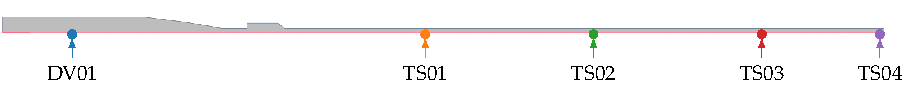
\includegraphics[width=5.75in]{../figures/STAR_new_geometry_colorlabels_tikz.pdf}};
    %\node[inner sep=0pt] (geom label) at (0,0) {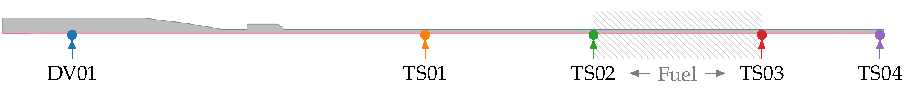
\includegraphics[width=5.75in]{../figures/STAR_new_geometry_colorlabels_fuel_tikz.pdf}};
    %\node[inner sep=0pt] (plot) at (0,-6){%% Creator: Matplotlib, PGF backend
%%
%% To include the figure in your LaTeX document, write
%%   \input{<filename>.pgf}
%%
%% Make sure the required packages are loaded in your preamble
%%   \usepackage{pgf}
%%
%% Also ensure that all the required font packages are loaded; for instance,
%% the lmodern package is sometimes necessary when using math font.
%%   \usepackage{lmodern}
%%
%% Figures using additional raster images can only be included by \input if
%% they are in the same directory as the main LaTeX file. For loading figures
%% from other directories you can use the `import` package
%%   \usepackage{import}
%%
%% and then include the figures with
%%   \import{<path to file>}{<filename>.pgf}
%%
%% Matplotlib used the following preamble
%%   \def\mathdefault#1{#1}
%%   \everymath=\expandafter{\the\everymath\displaystyle}
%%   \usepackage[utf8]{inputenc}
%%   \usepackage[T1]{fontenc}
%%   \usepackage[detect-all]{siunitx}
%%   \providecommand{\mathdefault}[1]{}
%%   \makeatletter\@ifpackageloaded{underscore}{}{\usepackage[strings]{underscore}}\makeatother
%%
\begingroup%
\makeatletter%
\begin{pgfpicture}%
\pgfpathrectangle{\pgfpointorigin}{\pgfqpoint{5.750000in}{4.312500in}}%
\pgfusepath{use as bounding box, clip}%
\begin{pgfscope}%
\pgfsetbuttcap%
\pgfsetmiterjoin%
\pgfsetlinewidth{0.000000pt}%
\definecolor{currentstroke}{rgb}{0.000000,0.000000,0.000000}%
\pgfsetstrokecolor{currentstroke}%
\pgfsetstrokeopacity{0.000000}%
\pgfsetdash{}{0pt}%
\pgfpathmoveto{\pgfqpoint{0.000000in}{0.000000in}}%
\pgfpathlineto{\pgfqpoint{5.750000in}{0.000000in}}%
\pgfpathlineto{\pgfqpoint{5.750000in}{4.312500in}}%
\pgfpathlineto{\pgfqpoint{0.000000in}{4.312500in}}%
\pgfpathlineto{\pgfqpoint{0.000000in}{0.000000in}}%
\pgfpathclose%
\pgfusepath{}%
\end{pgfscope}%
\begin{pgfscope}%
\pgfsetbuttcap%
\pgfsetmiterjoin%
\pgfsetlinewidth{0.000000pt}%
\definecolor{currentstroke}{rgb}{0.000000,0.000000,0.000000}%
\pgfsetstrokecolor{currentstroke}%
\pgfsetstrokeopacity{0.000000}%
\pgfsetdash{}{0pt}%
\pgfpathmoveto{\pgfqpoint{0.726769in}{0.580216in}}%
\pgfpathlineto{\pgfqpoint{5.585000in}{0.580216in}}%
\pgfpathlineto{\pgfqpoint{5.585000in}{4.147500in}}%
\pgfpathlineto{\pgfqpoint{0.726769in}{4.147500in}}%
\pgfpathlineto{\pgfqpoint{0.726769in}{0.580216in}}%
\pgfpathclose%
\pgfusepath{}%
\end{pgfscope}%
\begin{pgfscope}%
\pgfpathrectangle{\pgfqpoint{0.726769in}{0.580216in}}{\pgfqpoint{4.858231in}{3.567284in}}%
\pgfusepath{clip}%
\pgfsetrectcap%
\pgfsetroundjoin%
\pgfsetlinewidth{0.803000pt}%
\definecolor{currentstroke}{rgb}{0.690196,0.690196,0.690196}%
\pgfsetstrokecolor{currentstroke}%
\pgfsetdash{}{0pt}%
\pgfpathmoveto{\pgfqpoint{0.947576in}{0.580216in}}%
\pgfpathlineto{\pgfqpoint{0.947576in}{4.147500in}}%
\pgfusepath{stroke}%
\end{pgfscope}%
\begin{pgfscope}%
\pgfsetbuttcap%
\pgfsetroundjoin%
\definecolor{currentfill}{rgb}{0.000000,0.000000,0.000000}%
\pgfsetfillcolor{currentfill}%
\pgfsetlinewidth{0.803000pt}%
\definecolor{currentstroke}{rgb}{0.000000,0.000000,0.000000}%
\pgfsetstrokecolor{currentstroke}%
\pgfsetdash{}{0pt}%
\pgfsys@defobject{currentmarker}{\pgfqpoint{0.000000in}{-0.048611in}}{\pgfqpoint{0.000000in}{0.000000in}}{%
\pgfpathmoveto{\pgfqpoint{0.000000in}{0.000000in}}%
\pgfpathlineto{\pgfqpoint{0.000000in}{-0.048611in}}%
\pgfusepath{stroke,fill}%
}%
\begin{pgfscope}%
\pgfsys@transformshift{0.947576in}{0.580216in}%
\pgfsys@useobject{currentmarker}{}%
\end{pgfscope}%
\end{pgfscope}%
\begin{pgfscope}%
\definecolor{textcolor}{rgb}{0.000000,0.000000,0.000000}%
\pgfsetstrokecolor{textcolor}%
\pgfsetfillcolor{textcolor}%
\pgftext[x=0.947576in,y=0.482994in,,top]{\color{textcolor}{\rmfamily\fontsize{9.000000}{10.800000}\selectfont\catcode`\^=\active\def^{\ifmmode\sp\else\^{}\fi}\catcode`\%=\active\def%{\%}$\mathdefault{0.000}$}}%
\end{pgfscope}%
\begin{pgfscope}%
\pgfpathrectangle{\pgfqpoint{0.726769in}{0.580216in}}{\pgfqpoint{4.858231in}{3.567284in}}%
\pgfusepath{clip}%
\pgfsetrectcap%
\pgfsetroundjoin%
\pgfsetlinewidth{0.803000pt}%
\definecolor{currentstroke}{rgb}{0.690196,0.690196,0.690196}%
\pgfsetstrokecolor{currentstroke}%
\pgfsetdash{}{0pt}%
\pgfpathmoveto{\pgfqpoint{1.830899in}{0.580216in}}%
\pgfpathlineto{\pgfqpoint{1.830899in}{4.147500in}}%
\pgfusepath{stroke}%
\end{pgfscope}%
\begin{pgfscope}%
\pgfsetbuttcap%
\pgfsetroundjoin%
\definecolor{currentfill}{rgb}{0.000000,0.000000,0.000000}%
\pgfsetfillcolor{currentfill}%
\pgfsetlinewidth{0.803000pt}%
\definecolor{currentstroke}{rgb}{0.000000,0.000000,0.000000}%
\pgfsetstrokecolor{currentstroke}%
\pgfsetdash{}{0pt}%
\pgfsys@defobject{currentmarker}{\pgfqpoint{0.000000in}{-0.048611in}}{\pgfqpoint{0.000000in}{0.000000in}}{%
\pgfpathmoveto{\pgfqpoint{0.000000in}{0.000000in}}%
\pgfpathlineto{\pgfqpoint{0.000000in}{-0.048611in}}%
\pgfusepath{stroke,fill}%
}%
\begin{pgfscope}%
\pgfsys@transformshift{1.830899in}{0.580216in}%
\pgfsys@useobject{currentmarker}{}%
\end{pgfscope}%
\end{pgfscope}%
\begin{pgfscope}%
\definecolor{textcolor}{rgb}{0.000000,0.000000,0.000000}%
\pgfsetstrokecolor{textcolor}%
\pgfsetfillcolor{textcolor}%
\pgftext[x=1.830899in,y=0.482994in,,top]{\color{textcolor}{\rmfamily\fontsize{9.000000}{10.800000}\selectfont\catcode`\^=\active\def^{\ifmmode\sp\else\^{}\fi}\catcode`\%=\active\def%{\%}$\mathdefault{0.002}$}}%
\end{pgfscope}%
\begin{pgfscope}%
\pgfpathrectangle{\pgfqpoint{0.726769in}{0.580216in}}{\pgfqpoint{4.858231in}{3.567284in}}%
\pgfusepath{clip}%
\pgfsetrectcap%
\pgfsetroundjoin%
\pgfsetlinewidth{0.803000pt}%
\definecolor{currentstroke}{rgb}{0.690196,0.690196,0.690196}%
\pgfsetstrokecolor{currentstroke}%
\pgfsetdash{}{0pt}%
\pgfpathmoveto{\pgfqpoint{2.714223in}{0.580216in}}%
\pgfpathlineto{\pgfqpoint{2.714223in}{4.147500in}}%
\pgfusepath{stroke}%
\end{pgfscope}%
\begin{pgfscope}%
\pgfsetbuttcap%
\pgfsetroundjoin%
\definecolor{currentfill}{rgb}{0.000000,0.000000,0.000000}%
\pgfsetfillcolor{currentfill}%
\pgfsetlinewidth{0.803000pt}%
\definecolor{currentstroke}{rgb}{0.000000,0.000000,0.000000}%
\pgfsetstrokecolor{currentstroke}%
\pgfsetdash{}{0pt}%
\pgfsys@defobject{currentmarker}{\pgfqpoint{0.000000in}{-0.048611in}}{\pgfqpoint{0.000000in}{0.000000in}}{%
\pgfpathmoveto{\pgfqpoint{0.000000in}{0.000000in}}%
\pgfpathlineto{\pgfqpoint{0.000000in}{-0.048611in}}%
\pgfusepath{stroke,fill}%
}%
\begin{pgfscope}%
\pgfsys@transformshift{2.714223in}{0.580216in}%
\pgfsys@useobject{currentmarker}{}%
\end{pgfscope}%
\end{pgfscope}%
\begin{pgfscope}%
\definecolor{textcolor}{rgb}{0.000000,0.000000,0.000000}%
\pgfsetstrokecolor{textcolor}%
\pgfsetfillcolor{textcolor}%
\pgftext[x=2.714223in,y=0.482994in,,top]{\color{textcolor}{\rmfamily\fontsize{9.000000}{10.800000}\selectfont\catcode`\^=\active\def^{\ifmmode\sp\else\^{}\fi}\catcode`\%=\active\def%{\%}$\mathdefault{0.004}$}}%
\end{pgfscope}%
\begin{pgfscope}%
\pgfpathrectangle{\pgfqpoint{0.726769in}{0.580216in}}{\pgfqpoint{4.858231in}{3.567284in}}%
\pgfusepath{clip}%
\pgfsetrectcap%
\pgfsetroundjoin%
\pgfsetlinewidth{0.803000pt}%
\definecolor{currentstroke}{rgb}{0.690196,0.690196,0.690196}%
\pgfsetstrokecolor{currentstroke}%
\pgfsetdash{}{0pt}%
\pgfpathmoveto{\pgfqpoint{3.597546in}{0.580216in}}%
\pgfpathlineto{\pgfqpoint{3.597546in}{4.147500in}}%
\pgfusepath{stroke}%
\end{pgfscope}%
\begin{pgfscope}%
\pgfsetbuttcap%
\pgfsetroundjoin%
\definecolor{currentfill}{rgb}{0.000000,0.000000,0.000000}%
\pgfsetfillcolor{currentfill}%
\pgfsetlinewidth{0.803000pt}%
\definecolor{currentstroke}{rgb}{0.000000,0.000000,0.000000}%
\pgfsetstrokecolor{currentstroke}%
\pgfsetdash{}{0pt}%
\pgfsys@defobject{currentmarker}{\pgfqpoint{0.000000in}{-0.048611in}}{\pgfqpoint{0.000000in}{0.000000in}}{%
\pgfpathmoveto{\pgfqpoint{0.000000in}{0.000000in}}%
\pgfpathlineto{\pgfqpoint{0.000000in}{-0.048611in}}%
\pgfusepath{stroke,fill}%
}%
\begin{pgfscope}%
\pgfsys@transformshift{3.597546in}{0.580216in}%
\pgfsys@useobject{currentmarker}{}%
\end{pgfscope}%
\end{pgfscope}%
\begin{pgfscope}%
\definecolor{textcolor}{rgb}{0.000000,0.000000,0.000000}%
\pgfsetstrokecolor{textcolor}%
\pgfsetfillcolor{textcolor}%
\pgftext[x=3.597546in,y=0.482994in,,top]{\color{textcolor}{\rmfamily\fontsize{9.000000}{10.800000}\selectfont\catcode`\^=\active\def^{\ifmmode\sp\else\^{}\fi}\catcode`\%=\active\def%{\%}$\mathdefault{0.006}$}}%
\end{pgfscope}%
\begin{pgfscope}%
\pgfpathrectangle{\pgfqpoint{0.726769in}{0.580216in}}{\pgfqpoint{4.858231in}{3.567284in}}%
\pgfusepath{clip}%
\pgfsetrectcap%
\pgfsetroundjoin%
\pgfsetlinewidth{0.803000pt}%
\definecolor{currentstroke}{rgb}{0.690196,0.690196,0.690196}%
\pgfsetstrokecolor{currentstroke}%
\pgfsetdash{}{0pt}%
\pgfpathmoveto{\pgfqpoint{4.480870in}{0.580216in}}%
\pgfpathlineto{\pgfqpoint{4.480870in}{4.147500in}}%
\pgfusepath{stroke}%
\end{pgfscope}%
\begin{pgfscope}%
\pgfsetbuttcap%
\pgfsetroundjoin%
\definecolor{currentfill}{rgb}{0.000000,0.000000,0.000000}%
\pgfsetfillcolor{currentfill}%
\pgfsetlinewidth{0.803000pt}%
\definecolor{currentstroke}{rgb}{0.000000,0.000000,0.000000}%
\pgfsetstrokecolor{currentstroke}%
\pgfsetdash{}{0pt}%
\pgfsys@defobject{currentmarker}{\pgfqpoint{0.000000in}{-0.048611in}}{\pgfqpoint{0.000000in}{0.000000in}}{%
\pgfpathmoveto{\pgfqpoint{0.000000in}{0.000000in}}%
\pgfpathlineto{\pgfqpoint{0.000000in}{-0.048611in}}%
\pgfusepath{stroke,fill}%
}%
\begin{pgfscope}%
\pgfsys@transformshift{4.480870in}{0.580216in}%
\pgfsys@useobject{currentmarker}{}%
\end{pgfscope}%
\end{pgfscope}%
\begin{pgfscope}%
\definecolor{textcolor}{rgb}{0.000000,0.000000,0.000000}%
\pgfsetstrokecolor{textcolor}%
\pgfsetfillcolor{textcolor}%
\pgftext[x=4.480870in,y=0.482994in,,top]{\color{textcolor}{\rmfamily\fontsize{9.000000}{10.800000}\selectfont\catcode`\^=\active\def^{\ifmmode\sp\else\^{}\fi}\catcode`\%=\active\def%{\%}$\mathdefault{0.008}$}}%
\end{pgfscope}%
\begin{pgfscope}%
\pgfpathrectangle{\pgfqpoint{0.726769in}{0.580216in}}{\pgfqpoint{4.858231in}{3.567284in}}%
\pgfusepath{clip}%
\pgfsetrectcap%
\pgfsetroundjoin%
\pgfsetlinewidth{0.803000pt}%
\definecolor{currentstroke}{rgb}{0.690196,0.690196,0.690196}%
\pgfsetstrokecolor{currentstroke}%
\pgfsetdash{}{0pt}%
\pgfpathmoveto{\pgfqpoint{5.364193in}{0.580216in}}%
\pgfpathlineto{\pgfqpoint{5.364193in}{4.147500in}}%
\pgfusepath{stroke}%
\end{pgfscope}%
\begin{pgfscope}%
\pgfsetbuttcap%
\pgfsetroundjoin%
\definecolor{currentfill}{rgb}{0.000000,0.000000,0.000000}%
\pgfsetfillcolor{currentfill}%
\pgfsetlinewidth{0.803000pt}%
\definecolor{currentstroke}{rgb}{0.000000,0.000000,0.000000}%
\pgfsetstrokecolor{currentstroke}%
\pgfsetdash{}{0pt}%
\pgfsys@defobject{currentmarker}{\pgfqpoint{0.000000in}{-0.048611in}}{\pgfqpoint{0.000000in}{0.000000in}}{%
\pgfpathmoveto{\pgfqpoint{0.000000in}{0.000000in}}%
\pgfpathlineto{\pgfqpoint{0.000000in}{-0.048611in}}%
\pgfusepath{stroke,fill}%
}%
\begin{pgfscope}%
\pgfsys@transformshift{5.364193in}{0.580216in}%
\pgfsys@useobject{currentmarker}{}%
\end{pgfscope}%
\end{pgfscope}%
\begin{pgfscope}%
\definecolor{textcolor}{rgb}{0.000000,0.000000,0.000000}%
\pgfsetstrokecolor{textcolor}%
\pgfsetfillcolor{textcolor}%
\pgftext[x=5.364193in,y=0.482994in,,top]{\color{textcolor}{\rmfamily\fontsize{9.000000}{10.800000}\selectfont\catcode`\^=\active\def^{\ifmmode\sp\else\^{}\fi}\catcode`\%=\active\def%{\%}$\mathdefault{0.010}$}}%
\end{pgfscope}%
\begin{pgfscope}%
\definecolor{textcolor}{rgb}{0.000000,0.000000,0.000000}%
\pgfsetstrokecolor{textcolor}%
\pgfsetfillcolor{textcolor}%
\pgftext[x=3.155885in,y=0.317048in,,top]{\color{textcolor}{\rmfamily\fontsize{11.000000}{13.200000}\selectfont\catcode`\^=\active\def^{\ifmmode\sp\else\^{}\fi}\catcode`\%=\active\def%{\%}Time (\si{\second})}}%
\end{pgfscope}%
\begin{pgfscope}%
\pgfpathrectangle{\pgfqpoint{0.726769in}{0.580216in}}{\pgfqpoint{4.858231in}{3.567284in}}%
\pgfusepath{clip}%
\pgfsetrectcap%
\pgfsetroundjoin%
\pgfsetlinewidth{0.803000pt}%
\definecolor{currentstroke}{rgb}{0.690196,0.690196,0.690196}%
\pgfsetstrokecolor{currentstroke}%
\pgfsetdash{}{0pt}%
\pgfpathmoveto{\pgfqpoint{0.726769in}{0.649188in}}%
\pgfpathlineto{\pgfqpoint{5.585000in}{0.649188in}}%
\pgfusepath{stroke}%
\end{pgfscope}%
\begin{pgfscope}%
\pgfsetbuttcap%
\pgfsetroundjoin%
\definecolor{currentfill}{rgb}{0.000000,0.000000,0.000000}%
\pgfsetfillcolor{currentfill}%
\pgfsetlinewidth{0.803000pt}%
\definecolor{currentstroke}{rgb}{0.000000,0.000000,0.000000}%
\pgfsetstrokecolor{currentstroke}%
\pgfsetdash{}{0pt}%
\pgfsys@defobject{currentmarker}{\pgfqpoint{-0.048611in}{0.000000in}}{\pgfqpoint{-0.000000in}{0.000000in}}{%
\pgfpathmoveto{\pgfqpoint{-0.000000in}{0.000000in}}%
\pgfpathlineto{\pgfqpoint{-0.048611in}{0.000000in}}%
\pgfusepath{stroke,fill}%
}%
\begin{pgfscope}%
\pgfsys@transformshift{0.726769in}{0.649188in}%
\pgfsys@useobject{currentmarker}{}%
\end{pgfscope}%
\end{pgfscope}%
\begin{pgfscope}%
\definecolor{textcolor}{rgb}{0.000000,0.000000,0.000000}%
\pgfsetstrokecolor{textcolor}%
\pgfsetfillcolor{textcolor}%
\pgftext[x=0.565311in, y=0.606143in, left, base]{\color{textcolor}{\rmfamily\fontsize{9.000000}{10.800000}\selectfont\catcode`\^=\active\def^{\ifmmode\sp\else\^{}\fi}\catcode`\%=\active\def%{\%}$\mathdefault{0}$}}%
\end{pgfscope}%
\begin{pgfscope}%
\pgfpathrectangle{\pgfqpoint{0.726769in}{0.580216in}}{\pgfqpoint{4.858231in}{3.567284in}}%
\pgfusepath{clip}%
\pgfsetrectcap%
\pgfsetroundjoin%
\pgfsetlinewidth{0.803000pt}%
\definecolor{currentstroke}{rgb}{0.690196,0.690196,0.690196}%
\pgfsetstrokecolor{currentstroke}%
\pgfsetdash{}{0pt}%
\pgfpathmoveto{\pgfqpoint{0.726769in}{1.215067in}}%
\pgfpathlineto{\pgfqpoint{5.585000in}{1.215067in}}%
\pgfusepath{stroke}%
\end{pgfscope}%
\begin{pgfscope}%
\pgfsetbuttcap%
\pgfsetroundjoin%
\definecolor{currentfill}{rgb}{0.000000,0.000000,0.000000}%
\pgfsetfillcolor{currentfill}%
\pgfsetlinewidth{0.803000pt}%
\definecolor{currentstroke}{rgb}{0.000000,0.000000,0.000000}%
\pgfsetstrokecolor{currentstroke}%
\pgfsetdash{}{0pt}%
\pgfsys@defobject{currentmarker}{\pgfqpoint{-0.048611in}{0.000000in}}{\pgfqpoint{-0.000000in}{0.000000in}}{%
\pgfpathmoveto{\pgfqpoint{-0.000000in}{0.000000in}}%
\pgfpathlineto{\pgfqpoint{-0.048611in}{0.000000in}}%
\pgfusepath{stroke,fill}%
}%
\begin{pgfscope}%
\pgfsys@transformshift{0.726769in}{1.215067in}%
\pgfsys@useobject{currentmarker}{}%
\end{pgfscope}%
\end{pgfscope}%
\begin{pgfscope}%
\definecolor{textcolor}{rgb}{0.000000,0.000000,0.000000}%
\pgfsetstrokecolor{textcolor}%
\pgfsetfillcolor{textcolor}%
\pgftext[x=0.436840in, y=1.172022in, left, base]{\color{textcolor}{\rmfamily\fontsize{9.000000}{10.800000}\selectfont\catcode`\^=\active\def^{\ifmmode\sp\else\^{}\fi}\catcode`\%=\active\def%{\%}$\mathdefault{500}$}}%
\end{pgfscope}%
\begin{pgfscope}%
\pgfpathrectangle{\pgfqpoint{0.726769in}{0.580216in}}{\pgfqpoint{4.858231in}{3.567284in}}%
\pgfusepath{clip}%
\pgfsetrectcap%
\pgfsetroundjoin%
\pgfsetlinewidth{0.803000pt}%
\definecolor{currentstroke}{rgb}{0.690196,0.690196,0.690196}%
\pgfsetstrokecolor{currentstroke}%
\pgfsetdash{}{0pt}%
\pgfpathmoveto{\pgfqpoint{0.726769in}{1.780945in}}%
\pgfpathlineto{\pgfqpoint{5.585000in}{1.780945in}}%
\pgfusepath{stroke}%
\end{pgfscope}%
\begin{pgfscope}%
\pgfsetbuttcap%
\pgfsetroundjoin%
\definecolor{currentfill}{rgb}{0.000000,0.000000,0.000000}%
\pgfsetfillcolor{currentfill}%
\pgfsetlinewidth{0.803000pt}%
\definecolor{currentstroke}{rgb}{0.000000,0.000000,0.000000}%
\pgfsetstrokecolor{currentstroke}%
\pgfsetdash{}{0pt}%
\pgfsys@defobject{currentmarker}{\pgfqpoint{-0.048611in}{0.000000in}}{\pgfqpoint{-0.000000in}{0.000000in}}{%
\pgfpathmoveto{\pgfqpoint{-0.000000in}{0.000000in}}%
\pgfpathlineto{\pgfqpoint{-0.048611in}{0.000000in}}%
\pgfusepath{stroke,fill}%
}%
\begin{pgfscope}%
\pgfsys@transformshift{0.726769in}{1.780945in}%
\pgfsys@useobject{currentmarker}{}%
\end{pgfscope}%
\end{pgfscope}%
\begin{pgfscope}%
\definecolor{textcolor}{rgb}{0.000000,0.000000,0.000000}%
\pgfsetstrokecolor{textcolor}%
\pgfsetfillcolor{textcolor}%
\pgftext[x=0.372604in, y=1.737900in, left, base]{\color{textcolor}{\rmfamily\fontsize{9.000000}{10.800000}\selectfont\catcode`\^=\active\def^{\ifmmode\sp\else\^{}\fi}\catcode`\%=\active\def%{\%}$\mathdefault{1000}$}}%
\end{pgfscope}%
\begin{pgfscope}%
\pgfpathrectangle{\pgfqpoint{0.726769in}{0.580216in}}{\pgfqpoint{4.858231in}{3.567284in}}%
\pgfusepath{clip}%
\pgfsetrectcap%
\pgfsetroundjoin%
\pgfsetlinewidth{0.803000pt}%
\definecolor{currentstroke}{rgb}{0.690196,0.690196,0.690196}%
\pgfsetstrokecolor{currentstroke}%
\pgfsetdash{}{0pt}%
\pgfpathmoveto{\pgfqpoint{0.726769in}{2.346824in}}%
\pgfpathlineto{\pgfqpoint{5.585000in}{2.346824in}}%
\pgfusepath{stroke}%
\end{pgfscope}%
\begin{pgfscope}%
\pgfsetbuttcap%
\pgfsetroundjoin%
\definecolor{currentfill}{rgb}{0.000000,0.000000,0.000000}%
\pgfsetfillcolor{currentfill}%
\pgfsetlinewidth{0.803000pt}%
\definecolor{currentstroke}{rgb}{0.000000,0.000000,0.000000}%
\pgfsetstrokecolor{currentstroke}%
\pgfsetdash{}{0pt}%
\pgfsys@defobject{currentmarker}{\pgfqpoint{-0.048611in}{0.000000in}}{\pgfqpoint{-0.000000in}{0.000000in}}{%
\pgfpathmoveto{\pgfqpoint{-0.000000in}{0.000000in}}%
\pgfpathlineto{\pgfqpoint{-0.048611in}{0.000000in}}%
\pgfusepath{stroke,fill}%
}%
\begin{pgfscope}%
\pgfsys@transformshift{0.726769in}{2.346824in}%
\pgfsys@useobject{currentmarker}{}%
\end{pgfscope}%
\end{pgfscope}%
\begin{pgfscope}%
\definecolor{textcolor}{rgb}{0.000000,0.000000,0.000000}%
\pgfsetstrokecolor{textcolor}%
\pgfsetfillcolor{textcolor}%
\pgftext[x=0.372604in, y=2.303779in, left, base]{\color{textcolor}{\rmfamily\fontsize{9.000000}{10.800000}\selectfont\catcode`\^=\active\def^{\ifmmode\sp\else\^{}\fi}\catcode`\%=\active\def%{\%}$\mathdefault{1500}$}}%
\end{pgfscope}%
\begin{pgfscope}%
\pgfpathrectangle{\pgfqpoint{0.726769in}{0.580216in}}{\pgfqpoint{4.858231in}{3.567284in}}%
\pgfusepath{clip}%
\pgfsetrectcap%
\pgfsetroundjoin%
\pgfsetlinewidth{0.803000pt}%
\definecolor{currentstroke}{rgb}{0.690196,0.690196,0.690196}%
\pgfsetstrokecolor{currentstroke}%
\pgfsetdash{}{0pt}%
\pgfpathmoveto{\pgfqpoint{0.726769in}{2.912702in}}%
\pgfpathlineto{\pgfqpoint{5.585000in}{2.912702in}}%
\pgfusepath{stroke}%
\end{pgfscope}%
\begin{pgfscope}%
\pgfsetbuttcap%
\pgfsetroundjoin%
\definecolor{currentfill}{rgb}{0.000000,0.000000,0.000000}%
\pgfsetfillcolor{currentfill}%
\pgfsetlinewidth{0.803000pt}%
\definecolor{currentstroke}{rgb}{0.000000,0.000000,0.000000}%
\pgfsetstrokecolor{currentstroke}%
\pgfsetdash{}{0pt}%
\pgfsys@defobject{currentmarker}{\pgfqpoint{-0.048611in}{0.000000in}}{\pgfqpoint{-0.000000in}{0.000000in}}{%
\pgfpathmoveto{\pgfqpoint{-0.000000in}{0.000000in}}%
\pgfpathlineto{\pgfqpoint{-0.048611in}{0.000000in}}%
\pgfusepath{stroke,fill}%
}%
\begin{pgfscope}%
\pgfsys@transformshift{0.726769in}{2.912702in}%
\pgfsys@useobject{currentmarker}{}%
\end{pgfscope}%
\end{pgfscope}%
\begin{pgfscope}%
\definecolor{textcolor}{rgb}{0.000000,0.000000,0.000000}%
\pgfsetstrokecolor{textcolor}%
\pgfsetfillcolor{textcolor}%
\pgftext[x=0.372604in, y=2.869657in, left, base]{\color{textcolor}{\rmfamily\fontsize{9.000000}{10.800000}\selectfont\catcode`\^=\active\def^{\ifmmode\sp\else\^{}\fi}\catcode`\%=\active\def%{\%}$\mathdefault{2000}$}}%
\end{pgfscope}%
\begin{pgfscope}%
\pgfpathrectangle{\pgfqpoint{0.726769in}{0.580216in}}{\pgfqpoint{4.858231in}{3.567284in}}%
\pgfusepath{clip}%
\pgfsetrectcap%
\pgfsetroundjoin%
\pgfsetlinewidth{0.803000pt}%
\definecolor{currentstroke}{rgb}{0.690196,0.690196,0.690196}%
\pgfsetstrokecolor{currentstroke}%
\pgfsetdash{}{0pt}%
\pgfpathmoveto{\pgfqpoint{0.726769in}{3.478581in}}%
\pgfpathlineto{\pgfqpoint{5.585000in}{3.478581in}}%
\pgfusepath{stroke}%
\end{pgfscope}%
\begin{pgfscope}%
\pgfsetbuttcap%
\pgfsetroundjoin%
\definecolor{currentfill}{rgb}{0.000000,0.000000,0.000000}%
\pgfsetfillcolor{currentfill}%
\pgfsetlinewidth{0.803000pt}%
\definecolor{currentstroke}{rgb}{0.000000,0.000000,0.000000}%
\pgfsetstrokecolor{currentstroke}%
\pgfsetdash{}{0pt}%
\pgfsys@defobject{currentmarker}{\pgfqpoint{-0.048611in}{0.000000in}}{\pgfqpoint{-0.000000in}{0.000000in}}{%
\pgfpathmoveto{\pgfqpoint{-0.000000in}{0.000000in}}%
\pgfpathlineto{\pgfqpoint{-0.048611in}{0.000000in}}%
\pgfusepath{stroke,fill}%
}%
\begin{pgfscope}%
\pgfsys@transformshift{0.726769in}{3.478581in}%
\pgfsys@useobject{currentmarker}{}%
\end{pgfscope}%
\end{pgfscope}%
\begin{pgfscope}%
\definecolor{textcolor}{rgb}{0.000000,0.000000,0.000000}%
\pgfsetstrokecolor{textcolor}%
\pgfsetfillcolor{textcolor}%
\pgftext[x=0.372604in, y=3.435536in, left, base]{\color{textcolor}{\rmfamily\fontsize{9.000000}{10.800000}\selectfont\catcode`\^=\active\def^{\ifmmode\sp\else\^{}\fi}\catcode`\%=\active\def%{\%}$\mathdefault{2500}$}}%
\end{pgfscope}%
\begin{pgfscope}%
\pgfpathrectangle{\pgfqpoint{0.726769in}{0.580216in}}{\pgfqpoint{4.858231in}{3.567284in}}%
\pgfusepath{clip}%
\pgfsetrectcap%
\pgfsetroundjoin%
\pgfsetlinewidth{0.803000pt}%
\definecolor{currentstroke}{rgb}{0.690196,0.690196,0.690196}%
\pgfsetstrokecolor{currentstroke}%
\pgfsetdash{}{0pt}%
\pgfpathmoveto{\pgfqpoint{0.726769in}{4.044459in}}%
\pgfpathlineto{\pgfqpoint{5.585000in}{4.044459in}}%
\pgfusepath{stroke}%
\end{pgfscope}%
\begin{pgfscope}%
\pgfsetbuttcap%
\pgfsetroundjoin%
\definecolor{currentfill}{rgb}{0.000000,0.000000,0.000000}%
\pgfsetfillcolor{currentfill}%
\pgfsetlinewidth{0.803000pt}%
\definecolor{currentstroke}{rgb}{0.000000,0.000000,0.000000}%
\pgfsetstrokecolor{currentstroke}%
\pgfsetdash{}{0pt}%
\pgfsys@defobject{currentmarker}{\pgfqpoint{-0.048611in}{0.000000in}}{\pgfqpoint{-0.000000in}{0.000000in}}{%
\pgfpathmoveto{\pgfqpoint{-0.000000in}{0.000000in}}%
\pgfpathlineto{\pgfqpoint{-0.048611in}{0.000000in}}%
\pgfusepath{stroke,fill}%
}%
\begin{pgfscope}%
\pgfsys@transformshift{0.726769in}{4.044459in}%
\pgfsys@useobject{currentmarker}{}%
\end{pgfscope}%
\end{pgfscope}%
\begin{pgfscope}%
\definecolor{textcolor}{rgb}{0.000000,0.000000,0.000000}%
\pgfsetstrokecolor{textcolor}%
\pgfsetfillcolor{textcolor}%
\pgftext[x=0.372604in, y=4.001414in, left, base]{\color{textcolor}{\rmfamily\fontsize{9.000000}{10.800000}\selectfont\catcode`\^=\active\def^{\ifmmode\sp\else\^{}\fi}\catcode`\%=\active\def%{\%}$\mathdefault{3000}$}}%
\end{pgfscope}%
\begin{pgfscope}%
\definecolor{textcolor}{rgb}{0.000000,0.000000,0.000000}%
\pgfsetstrokecolor{textcolor}%
\pgfsetfillcolor{textcolor}%
\pgftext[x=0.317048in,y=2.363858in,,bottom,rotate=90.000000]{\color{textcolor}{\rmfamily\fontsize{11.000000}{13.200000}\selectfont\catcode`\^=\active\def^{\ifmmode\sp\else\^{}\fi}\catcode`\%=\active\def%{\%}Temperature (\si{\kelvin})}}%
\end{pgfscope}%
\begin{pgfscope}%
\pgfpathrectangle{\pgfqpoint{0.726769in}{0.580216in}}{\pgfqpoint{4.858231in}{3.567284in}}%
\pgfusepath{clip}%
\pgfsetrectcap%
\pgfsetroundjoin%
\pgfsetlinewidth{1.505625pt}%
\definecolor{currentstroke}{rgb}{0.121569,0.466667,0.705882}%
\pgfsetstrokecolor{currentstroke}%
\pgfsetdash{}{0pt}%
\pgfpathmoveto{\pgfqpoint{0.947598in}{0.981472in}}%
\pgfpathlineto{\pgfqpoint{1.030255in}{0.981470in}}%
\pgfpathlineto{\pgfqpoint{1.032110in}{0.979405in}}%
\pgfpathlineto{\pgfqpoint{1.036747in}{0.975685in}}%
\pgfpathlineto{\pgfqpoint{1.041407in}{0.973083in}}%
\pgfpathlineto{\pgfqpoint{1.046972in}{0.971134in}}%
\pgfpathlineto{\pgfqpoint{1.055341in}{0.970413in}}%
\pgfpathlineto{\pgfqpoint{1.075768in}{0.972271in}}%
\pgfpathlineto{\pgfqpoint{1.076695in}{0.975586in}}%
\pgfpathlineto{\pgfqpoint{1.077623in}{0.975947in}}%
\pgfpathlineto{\pgfqpoint{1.079478in}{0.975172in}}%
\pgfpathlineto{\pgfqpoint{1.080405in}{0.974899in}}%
\pgfpathlineto{\pgfqpoint{1.082260in}{0.975086in}}%
\pgfpathlineto{\pgfqpoint{1.084115in}{0.974417in}}%
\pgfpathlineto{\pgfqpoint{1.087847in}{0.974030in}}%
\pgfpathlineto{\pgfqpoint{1.089702in}{0.974452in}}%
\pgfpathlineto{\pgfqpoint{1.094340in}{0.970791in}}%
\pgfpathlineto{\pgfqpoint{1.102709in}{0.965731in}}%
\pgfpathlineto{\pgfqpoint{1.110129in}{0.963119in}}%
\pgfpathlineto{\pgfqpoint{1.117571in}{0.961962in}}%
\pgfpathlineto{\pgfqpoint{1.120354in}{0.962114in}}%
\pgfpathlineto{\pgfqpoint{1.124064in}{0.962139in}}%
\pgfpathlineto{\pgfqpoint{1.127774in}{0.962674in}}%
\pgfpathlineto{\pgfqpoint{1.132433in}{0.963073in}}%
\pgfpathlineto{\pgfqpoint{1.137071in}{0.963765in}}%
\pgfpathlineto{\pgfqpoint{1.137998in}{0.963166in}}%
\pgfpathlineto{\pgfqpoint{1.138926in}{0.966518in}}%
\pgfpathlineto{\pgfqpoint{1.139853in}{0.966985in}}%
\pgfpathlineto{\pgfqpoint{1.141708in}{0.966558in}}%
\pgfpathlineto{\pgfqpoint{1.143563in}{0.966427in}}%
\pgfpathlineto{\pgfqpoint{1.146368in}{0.966261in}}%
\pgfpathlineto{\pgfqpoint{1.148223in}{0.966088in}}%
\pgfpathlineto{\pgfqpoint{1.152860in}{0.965633in}}%
\pgfpathlineto{\pgfqpoint{1.162157in}{0.964647in}}%
\pgfpathlineto{\pgfqpoint{1.164012in}{0.964696in}}%
\pgfpathlineto{\pgfqpoint{1.166794in}{0.964359in}}%
\pgfpathlineto{\pgfqpoint{1.175142in}{0.962944in}}%
\pgfpathlineto{\pgfqpoint{1.178874in}{0.962636in}}%
\pgfpathlineto{\pgfqpoint{1.187221in}{0.961285in}}%
\pgfpathlineto{\pgfqpoint{1.190931in}{0.961088in}}%
\pgfpathlineto{\pgfqpoint{1.193736in}{0.960527in}}%
\pgfpathlineto{\pgfqpoint{1.202083in}{0.959427in}}%
\pgfpathlineto{\pgfqpoint{1.206743in}{0.959079in}}%
\pgfpathlineto{\pgfqpoint{1.209525in}{0.958810in}}%
\pgfpathlineto{\pgfqpoint{1.217873in}{0.957217in}}%
\pgfpathlineto{\pgfqpoint{1.221605in}{0.956896in}}%
\pgfpathlineto{\pgfqpoint{1.224387in}{0.956170in}}%
\pgfpathlineto{\pgfqpoint{1.238322in}{0.953306in}}%
\pgfpathlineto{\pgfqpoint{1.242032in}{0.953153in}}%
\pgfpathlineto{\pgfqpoint{1.246669in}{0.953338in}}%
\pgfpathlineto{\pgfqpoint{1.252256in}{0.953434in}}%
\pgfpathlineto{\pgfqpoint{1.258748in}{0.954057in}}%
\pgfpathlineto{\pgfqpoint{1.265241in}{0.953495in}}%
\pgfpathlineto{\pgfqpoint{1.270828in}{0.953829in}}%
\pgfpathlineto{\pgfqpoint{1.276393in}{0.953339in}}%
\pgfpathlineto{\pgfqpoint{1.282907in}{0.951091in}}%
\pgfpathlineto{\pgfqpoint{1.286617in}{0.950589in}}%
\pgfpathlineto{\pgfqpoint{1.288472in}{0.950072in}}%
\pgfpathlineto{\pgfqpoint{1.290327in}{0.948717in}}%
\pgfpathlineto{\pgfqpoint{1.293110in}{0.948687in}}%
\pgfpathlineto{\pgfqpoint{1.304262in}{0.947449in}}%
\pgfpathlineto{\pgfqpoint{1.307972in}{0.947268in}}%
\pgfpathlineto{\pgfqpoint{1.311682in}{0.947753in}}%
\pgfpathlineto{\pgfqpoint{1.317269in}{0.948284in}}%
\pgfpathlineto{\pgfqpoint{1.322834in}{0.949807in}}%
\pgfpathlineto{\pgfqpoint{1.325616in}{0.949700in}}%
\pgfpathlineto{\pgfqpoint{1.328421in}{0.950281in}}%
\pgfpathlineto{\pgfqpoint{1.334913in}{0.951640in}}%
\pgfpathlineto{\pgfqpoint{1.336768in}{0.952062in}}%
\pgfpathlineto{\pgfqpoint{1.359072in}{0.946344in}}%
\pgfpathlineto{\pgfqpoint{1.361854in}{0.945735in}}%
\pgfpathlineto{\pgfqpoint{1.363709in}{0.945136in}}%
\pgfpathlineto{\pgfqpoint{1.365564in}{0.944972in}}%
\pgfpathlineto{\pgfqpoint{1.367419in}{0.944420in}}%
\pgfpathlineto{\pgfqpoint{1.372057in}{0.944445in}}%
\pgfpathlineto{\pgfqpoint{1.374861in}{0.943634in}}%
\pgfpathlineto{\pgfqpoint{1.376716in}{0.943531in}}%
\pgfpathlineto{\pgfqpoint{1.379499in}{0.942930in}}%
\pgfpathlineto{\pgfqpoint{1.382281in}{0.942307in}}%
\pgfpathlineto{\pgfqpoint{1.383209in}{0.942048in}}%
\pgfpathlineto{\pgfqpoint{1.385991in}{0.942316in}}%
\pgfpathlineto{\pgfqpoint{1.392506in}{0.942212in}}%
\pgfpathlineto{\pgfqpoint{1.406440in}{0.941749in}}%
\pgfpathlineto{\pgfqpoint{1.412005in}{0.940364in}}%
\pgfpathlineto{\pgfqpoint{1.420375in}{0.939919in}}%
\pgfpathlineto{\pgfqpoint{1.423157in}{0.939699in}}%
\pgfpathlineto{\pgfqpoint{1.430577in}{0.938654in}}%
\pgfpathlineto{\pgfqpoint{1.434287in}{0.938657in}}%
\pgfpathlineto{\pgfqpoint{1.438019in}{0.938631in}}%
\pgfpathlineto{\pgfqpoint{1.442656in}{0.938604in}}%
\pgfpathlineto{\pgfqpoint{1.446366in}{0.938743in}}%
\pgfpathlineto{\pgfqpoint{1.455663in}{0.938293in}}%
\pgfpathlineto{\pgfqpoint{1.467743in}{0.937312in}}%
\pgfpathlineto{\pgfqpoint{1.471453in}{0.937232in}}%
\pgfpathlineto{\pgfqpoint{1.475163in}{0.936375in}}%
\pgfpathlineto{\pgfqpoint{1.482605in}{0.935587in}}%
\pgfpathlineto{\pgfqpoint{1.490025in}{0.935310in}}%
\pgfpathlineto{\pgfqpoint{1.494662in}{0.934885in}}%
\pgfpathlineto{\pgfqpoint{1.499322in}{0.934468in}}%
\pgfpathlineto{\pgfqpoint{1.507669in}{0.935136in}}%
\pgfpathlineto{\pgfqpoint{1.516966in}{0.935975in}}%
\pgfpathlineto{\pgfqpoint{1.528118in}{0.935129in}}%
\pgfpathlineto{\pgfqpoint{1.530900in}{0.934827in}}%
\pgfpathlineto{\pgfqpoint{1.534610in}{0.934596in}}%
\pgfpathlineto{\pgfqpoint{1.538320in}{0.933946in}}%
\pgfpathlineto{\pgfqpoint{1.543907in}{0.932183in}}%
\pgfpathlineto{\pgfqpoint{1.546690in}{0.931299in}}%
\pgfpathlineto{\pgfqpoint{1.548545in}{0.930843in}}%
\pgfpathlineto{\pgfqpoint{1.550400in}{0.930368in}}%
\pgfpathlineto{\pgfqpoint{1.553182in}{0.929469in}}%
\pgfpathlineto{\pgfqpoint{1.555037in}{0.929439in}}%
\pgfpathlineto{\pgfqpoint{1.560624in}{0.928642in}}%
\pgfpathlineto{\pgfqpoint{1.562479in}{0.928608in}}%
\pgfpathlineto{\pgfqpoint{1.568044in}{0.927923in}}%
\pgfpathlineto{\pgfqpoint{1.571776in}{0.927958in}}%
\pgfpathlineto{\pgfqpoint{1.589421in}{0.928098in}}%
\pgfpathlineto{\pgfqpoint{1.592203in}{0.928637in}}%
\pgfpathlineto{\pgfqpoint{1.593131in}{0.928388in}}%
\pgfpathlineto{\pgfqpoint{1.594058in}{0.935273in}}%
\pgfpathlineto{\pgfqpoint{1.594986in}{0.937231in}}%
\pgfpathlineto{\pgfqpoint{1.595913in}{0.937547in}}%
\pgfpathlineto{\pgfqpoint{1.596841in}{0.936900in}}%
\pgfpathlineto{\pgfqpoint{1.597768in}{0.935668in}}%
\pgfpathlineto{\pgfqpoint{1.598696in}{0.936237in}}%
\pgfpathlineto{\pgfqpoint{1.599623in}{0.937323in}}%
\pgfpathlineto{\pgfqpoint{1.600550in}{0.936530in}}%
\pgfpathlineto{\pgfqpoint{1.601478in}{0.936769in}}%
\pgfpathlineto{\pgfqpoint{1.602428in}{0.934671in}}%
\pgfpathlineto{\pgfqpoint{1.603355in}{0.933609in}}%
\pgfpathlineto{\pgfqpoint{1.604283in}{0.936077in}}%
\pgfpathlineto{\pgfqpoint{1.607065in}{0.935049in}}%
\pgfpathlineto{\pgfqpoint{1.608920in}{0.934658in}}%
\pgfpathlineto{\pgfqpoint{1.609847in}{0.935270in}}%
\pgfpathlineto{\pgfqpoint{1.610775in}{0.933563in}}%
\pgfpathlineto{\pgfqpoint{1.611702in}{0.934241in}}%
\pgfpathlineto{\pgfqpoint{1.613557in}{0.940006in}}%
\pgfpathlineto{\pgfqpoint{1.616340in}{0.937466in}}%
\pgfpathlineto{\pgfqpoint{1.617289in}{0.937507in}}%
\pgfpathlineto{\pgfqpoint{1.618217in}{0.938854in}}%
\pgfpathlineto{\pgfqpoint{1.620072in}{0.936747in}}%
\pgfpathlineto{\pgfqpoint{1.621927in}{0.936204in}}%
\pgfpathlineto{\pgfqpoint{1.623782in}{0.936548in}}%
\pgfpathlineto{\pgfqpoint{1.625637in}{0.936064in}}%
\pgfpathlineto{\pgfqpoint{1.628419in}{0.936252in}}%
\pgfpathlineto{\pgfqpoint{1.631202in}{0.935626in}}%
\pgfpathlineto{\pgfqpoint{1.633079in}{0.936700in}}%
\pgfpathlineto{\pgfqpoint{1.634006in}{0.937435in}}%
\pgfpathlineto{\pgfqpoint{1.635861in}{0.937515in}}%
\pgfpathlineto{\pgfqpoint{1.637716in}{0.938329in}}%
\pgfpathlineto{\pgfqpoint{1.640499in}{0.936693in}}%
\pgfpathlineto{\pgfqpoint{1.641426in}{0.936653in}}%
\pgfpathlineto{\pgfqpoint{1.643281in}{0.937696in}}%
\pgfpathlineto{\pgfqpoint{1.646991in}{0.936394in}}%
\pgfpathlineto{\pgfqpoint{1.647941in}{0.936824in}}%
\pgfpathlineto{\pgfqpoint{1.652578in}{0.935260in}}%
\pgfpathlineto{\pgfqpoint{1.653506in}{0.935952in}}%
\pgfpathlineto{\pgfqpoint{1.654433in}{0.936171in}}%
\pgfpathlineto{\pgfqpoint{1.658143in}{0.935637in}}%
\pgfpathlineto{\pgfqpoint{1.659071in}{0.936293in}}%
\pgfpathlineto{\pgfqpoint{1.660926in}{0.945303in}}%
\pgfpathlineto{\pgfqpoint{1.662803in}{0.943812in}}%
\pgfpathlineto{\pgfqpoint{1.663730in}{0.944736in}}%
\pgfpathlineto{\pgfqpoint{1.666513in}{0.944646in}}%
\pgfpathlineto{\pgfqpoint{1.667440in}{0.943243in}}%
\pgfpathlineto{\pgfqpoint{1.668368in}{0.943113in}}%
\pgfpathlineto{\pgfqpoint{1.669295in}{0.943791in}}%
\pgfpathlineto{\pgfqpoint{1.672078in}{0.943088in}}%
\pgfpathlineto{\pgfqpoint{1.673005in}{0.943782in}}%
\pgfpathlineto{\pgfqpoint{1.673933in}{0.943603in}}%
\pgfpathlineto{\pgfqpoint{1.675788in}{0.942251in}}%
\pgfpathlineto{\pgfqpoint{1.676715in}{0.948577in}}%
\pgfpathlineto{\pgfqpoint{1.677643in}{0.949206in}}%
\pgfpathlineto{\pgfqpoint{1.678592in}{0.948106in}}%
\pgfpathlineto{\pgfqpoint{1.683230in}{0.946767in}}%
\pgfpathlineto{\pgfqpoint{1.689722in}{0.946579in}}%
\pgfpathlineto{\pgfqpoint{1.695309in}{0.946511in}}%
\pgfpathlineto{\pgfqpoint{1.697164in}{0.947876in}}%
\pgfpathlineto{\pgfqpoint{1.698091in}{0.947395in}}%
\pgfpathlineto{\pgfqpoint{1.700874in}{0.948767in}}%
\pgfpathlineto{\pgfqpoint{1.701801in}{0.948363in}}%
\pgfpathlineto{\pgfqpoint{1.703656in}{0.946702in}}%
\pgfpathlineto{\pgfqpoint{1.706439in}{0.947478in}}%
\pgfpathlineto{\pgfqpoint{1.709243in}{0.946138in}}%
\pgfpathlineto{\pgfqpoint{1.711098in}{0.946712in}}%
\pgfpathlineto{\pgfqpoint{1.713881in}{0.945031in}}%
\pgfpathlineto{\pgfqpoint{1.715736in}{0.944478in}}%
\pgfpathlineto{\pgfqpoint{1.719446in}{0.944676in}}%
\pgfpathlineto{\pgfqpoint{1.722228in}{0.943547in}}%
\pgfpathlineto{\pgfqpoint{1.724105in}{0.944457in}}%
\pgfpathlineto{\pgfqpoint{1.727815in}{0.943484in}}%
\pgfpathlineto{\pgfqpoint{1.730598in}{0.943593in}}%
\pgfpathlineto{\pgfqpoint{1.732453in}{0.943200in}}%
\pgfpathlineto{\pgfqpoint{1.733380in}{0.942873in}}%
\pgfpathlineto{\pgfqpoint{1.735235in}{0.943162in}}%
\pgfpathlineto{\pgfqpoint{1.739895in}{0.941974in}}%
\pgfpathlineto{\pgfqpoint{1.741750in}{0.942747in}}%
\pgfpathlineto{\pgfqpoint{1.745460in}{0.942807in}}%
\pgfpathlineto{\pgfqpoint{1.748242in}{0.942680in}}%
\pgfpathlineto{\pgfqpoint{1.750097in}{0.943030in}}%
\pgfpathlineto{\pgfqpoint{1.752880in}{0.942869in}}%
\pgfpathlineto{\pgfqpoint{1.755684in}{0.943602in}}%
\pgfpathlineto{\pgfqpoint{1.759394in}{0.943546in}}%
\pgfpathlineto{\pgfqpoint{1.762177in}{0.943577in}}%
\pgfpathlineto{\pgfqpoint{1.764032in}{0.943699in}}%
\pgfpathlineto{\pgfqpoint{1.765887in}{0.944274in}}%
\pgfpathlineto{\pgfqpoint{1.767742in}{0.944326in}}%
\pgfpathlineto{\pgfqpoint{1.769619in}{0.945020in}}%
\pgfpathlineto{\pgfqpoint{1.771474in}{0.944996in}}%
\pgfpathlineto{\pgfqpoint{1.778894in}{0.946647in}}%
\pgfpathlineto{\pgfqpoint{1.782603in}{0.947302in}}%
\pgfpathlineto{\pgfqpoint{1.785408in}{0.947829in}}%
\pgfpathlineto{\pgfqpoint{1.788190in}{0.948823in}}%
\pgfpathlineto{\pgfqpoint{1.790973in}{0.949441in}}%
\pgfpathlineto{\pgfqpoint{1.792828in}{0.950326in}}%
\pgfpathlineto{\pgfqpoint{1.795610in}{0.948917in}}%
\pgfpathlineto{\pgfqpoint{1.797465in}{0.949491in}}%
\pgfpathlineto{\pgfqpoint{1.798393in}{0.950392in}}%
\pgfpathlineto{\pgfqpoint{1.799320in}{0.950507in}}%
\pgfpathlineto{\pgfqpoint{1.800270in}{0.949377in}}%
\pgfpathlineto{\pgfqpoint{1.801197in}{0.948973in}}%
\pgfpathlineto{\pgfqpoint{1.803052in}{0.949155in}}%
\pgfpathlineto{\pgfqpoint{1.803980in}{0.950218in}}%
\pgfpathlineto{\pgfqpoint{1.804907in}{0.950190in}}%
\pgfpathlineto{\pgfqpoint{1.805835in}{0.948607in}}%
\pgfpathlineto{\pgfqpoint{1.806762in}{0.947884in}}%
\pgfpathlineto{\pgfqpoint{1.807690in}{0.948553in}}%
\pgfpathlineto{\pgfqpoint{1.808617in}{0.950067in}}%
\pgfpathlineto{\pgfqpoint{1.809545in}{0.949989in}}%
\pgfpathlineto{\pgfqpoint{1.810472in}{0.948924in}}%
\pgfpathlineto{\pgfqpoint{1.812327in}{0.949099in}}%
\pgfpathlineto{\pgfqpoint{1.813255in}{0.947926in}}%
\pgfpathlineto{\pgfqpoint{1.814182in}{0.947580in}}%
\pgfpathlineto{\pgfqpoint{1.816059in}{0.949249in}}%
\pgfpathlineto{\pgfqpoint{1.817914in}{0.947540in}}%
\pgfpathlineto{\pgfqpoint{1.821624in}{0.946074in}}%
\pgfpathlineto{\pgfqpoint{1.822552in}{0.946135in}}%
\pgfpathlineto{\pgfqpoint{1.823479in}{0.946752in}}%
\pgfpathlineto{\pgfqpoint{1.831849in}{0.946760in}}%
\pgfpathlineto{\pgfqpoint{1.833704in}{0.946679in}}%
\pgfpathlineto{\pgfqpoint{1.836486in}{0.947504in}}%
\pgfpathlineto{\pgfqpoint{1.839269in}{0.949561in}}%
\pgfpathlineto{\pgfqpoint{1.842051in}{0.950153in}}%
\pgfpathlineto{\pgfqpoint{1.844834in}{0.951459in}}%
\pgfpathlineto{\pgfqpoint{1.848566in}{0.952405in}}%
\pgfpathlineto{\pgfqpoint{1.852276in}{0.954591in}}%
\pgfpathlineto{\pgfqpoint{1.855986in}{0.954894in}}%
\pgfpathlineto{\pgfqpoint{1.856913in}{0.955602in}}%
\pgfpathlineto{\pgfqpoint{1.858768in}{0.955424in}}%
\pgfpathlineto{\pgfqpoint{1.859696in}{0.956444in}}%
\pgfpathlineto{\pgfqpoint{1.860645in}{0.956195in}}%
\pgfpathlineto{\pgfqpoint{1.861573in}{0.955516in}}%
\pgfpathlineto{\pgfqpoint{1.862500in}{0.955604in}}%
\pgfpathlineto{\pgfqpoint{1.864355in}{0.957687in}}%
\pgfpathlineto{\pgfqpoint{1.866210in}{0.955068in}}%
\pgfpathlineto{\pgfqpoint{1.867138in}{0.954899in}}%
\pgfpathlineto{\pgfqpoint{1.869920in}{0.957178in}}%
\pgfpathlineto{\pgfqpoint{1.870847in}{0.955976in}}%
\pgfpathlineto{\pgfqpoint{1.871775in}{0.954045in}}%
\pgfpathlineto{\pgfqpoint{1.872702in}{0.953910in}}%
\pgfpathlineto{\pgfqpoint{1.874557in}{0.957679in}}%
\pgfpathlineto{\pgfqpoint{1.875507in}{0.956593in}}%
\pgfpathlineto{\pgfqpoint{1.876435in}{0.954791in}}%
\pgfpathlineto{\pgfqpoint{1.877362in}{0.954301in}}%
\pgfpathlineto{\pgfqpoint{1.880144in}{0.955390in}}%
\pgfpathlineto{\pgfqpoint{1.881072in}{0.954769in}}%
\pgfpathlineto{\pgfqpoint{1.882927in}{0.952675in}}%
\pgfpathlineto{\pgfqpoint{1.886637in}{0.951815in}}%
\pgfpathlineto{\pgfqpoint{1.889419in}{0.953735in}}%
\pgfpathlineto{\pgfqpoint{1.890347in}{0.953278in}}%
\pgfpathlineto{\pgfqpoint{1.892224in}{0.951559in}}%
\pgfpathlineto{\pgfqpoint{1.896861in}{0.950927in}}%
\pgfpathlineto{\pgfqpoint{1.899644in}{0.949499in}}%
\pgfpathlineto{\pgfqpoint{1.900571in}{0.950009in}}%
\pgfpathlineto{\pgfqpoint{1.902426in}{0.951632in}}%
\pgfpathlineto{\pgfqpoint{1.904281in}{0.950680in}}%
\pgfpathlineto{\pgfqpoint{1.906158in}{0.950368in}}%
\pgfpathlineto{\pgfqpoint{1.907086in}{0.950889in}}%
\pgfpathlineto{\pgfqpoint{1.908013in}{0.952146in}}%
\pgfpathlineto{\pgfqpoint{1.908941in}{0.952657in}}%
\pgfpathlineto{\pgfqpoint{1.911723in}{0.951940in}}%
\pgfpathlineto{\pgfqpoint{1.914506in}{0.952591in}}%
\pgfpathlineto{\pgfqpoint{1.915433in}{0.952792in}}%
\pgfpathlineto{\pgfqpoint{1.919143in}{0.952024in}}%
\pgfpathlineto{\pgfqpoint{1.920998in}{0.953084in}}%
\pgfpathlineto{\pgfqpoint{1.922875in}{0.953394in}}%
\pgfpathlineto{\pgfqpoint{1.923803in}{0.954115in}}%
\pgfpathlineto{\pgfqpoint{1.924730in}{0.954141in}}%
\pgfpathlineto{\pgfqpoint{1.925658in}{0.953689in}}%
\pgfpathlineto{\pgfqpoint{1.926585in}{0.953930in}}%
\pgfpathlineto{\pgfqpoint{1.927513in}{0.955329in}}%
\pgfpathlineto{\pgfqpoint{1.928440in}{0.955319in}}%
\pgfpathlineto{\pgfqpoint{1.930295in}{0.954458in}}%
\pgfpathlineto{\pgfqpoint{1.933078in}{0.955295in}}%
\pgfpathlineto{\pgfqpoint{1.935860in}{0.955563in}}%
\pgfpathlineto{\pgfqpoint{1.936810in}{0.955938in}}%
\pgfpathlineto{\pgfqpoint{1.937737in}{0.957188in}}%
\pgfpathlineto{\pgfqpoint{1.938665in}{0.957790in}}%
\pgfpathlineto{\pgfqpoint{1.939592in}{0.957541in}}%
\pgfpathlineto{\pgfqpoint{1.940520in}{0.957697in}}%
\pgfpathlineto{\pgfqpoint{1.941447in}{0.958497in}}%
\pgfpathlineto{\pgfqpoint{1.942375in}{0.958673in}}%
\pgfpathlineto{\pgfqpoint{1.944230in}{0.957721in}}%
\pgfpathlineto{\pgfqpoint{1.948867in}{0.959103in}}%
\pgfpathlineto{\pgfqpoint{1.950722in}{0.959076in}}%
\pgfpathlineto{\pgfqpoint{1.952599in}{0.959847in}}%
\pgfpathlineto{\pgfqpoint{1.955382in}{0.958938in}}%
\pgfpathlineto{\pgfqpoint{1.957237in}{0.958993in}}%
\pgfpathlineto{\pgfqpoint{1.959092in}{0.958649in}}%
\pgfpathlineto{\pgfqpoint{1.961874in}{0.959215in}}%
\pgfpathlineto{\pgfqpoint{1.965584in}{0.958484in}}%
\pgfpathlineto{\pgfqpoint{1.967461in}{0.959490in}}%
\pgfpathlineto{\pgfqpoint{1.972098in}{0.958814in}}%
\pgfpathlineto{\pgfqpoint{1.974881in}{0.959407in}}%
\pgfpathlineto{\pgfqpoint{1.977663in}{0.958217in}}%
\pgfpathlineto{\pgfqpoint{1.980446in}{0.959010in}}%
\pgfpathlineto{\pgfqpoint{1.984178in}{0.957728in}}%
\pgfpathlineto{\pgfqpoint{1.987888in}{0.957493in}}%
\pgfpathlineto{\pgfqpoint{1.988815in}{0.957175in}}%
\pgfpathlineto{\pgfqpoint{1.990670in}{0.957420in}}%
\pgfpathlineto{\pgfqpoint{1.999040in}{0.956015in}}%
\pgfpathlineto{\pgfqpoint{2.000895in}{0.956427in}}%
\pgfpathlineto{\pgfqpoint{2.003677in}{0.956207in}}%
\pgfpathlineto{\pgfqpoint{2.004605in}{0.956406in}}%
\pgfpathlineto{\pgfqpoint{2.008315in}{0.955779in}}%
\pgfpathlineto{\pgfqpoint{2.012025in}{0.956094in}}%
\pgfpathlineto{\pgfqpoint{2.017612in}{0.957249in}}%
\pgfpathlineto{\pgfqpoint{2.021322in}{0.957204in}}%
\pgfpathlineto{\pgfqpoint{2.030619in}{0.959041in}}%
\pgfpathlineto{\pgfqpoint{2.033401in}{0.959172in}}%
\pgfpathlineto{\pgfqpoint{2.035256in}{0.959917in}}%
\pgfpathlineto{\pgfqpoint{2.037111in}{0.959602in}}%
\pgfpathlineto{\pgfqpoint{2.038966in}{0.959192in}}%
\pgfpathlineto{\pgfqpoint{2.042676in}{0.959190in}}%
\pgfpathlineto{\pgfqpoint{2.044553in}{0.958478in}}%
\pgfpathlineto{\pgfqpoint{2.047336in}{0.957055in}}%
\pgfpathlineto{\pgfqpoint{2.053828in}{0.955849in}}%
\pgfpathlineto{\pgfqpoint{2.055683in}{0.955845in}}%
\pgfpathlineto{\pgfqpoint{2.057538in}{0.954826in}}%
\pgfpathlineto{\pgfqpoint{2.059415in}{0.953423in}}%
\pgfpathlineto{\pgfqpoint{2.060342in}{0.953087in}}%
\pgfpathlineto{\pgfqpoint{2.061270in}{0.953163in}}%
\pgfpathlineto{\pgfqpoint{2.062197in}{0.953635in}}%
\pgfpathlineto{\pgfqpoint{2.063125in}{0.955404in}}%
\pgfpathlineto{\pgfqpoint{2.064052in}{0.955496in}}%
\pgfpathlineto{\pgfqpoint{2.065907in}{0.954133in}}%
\pgfpathlineto{\pgfqpoint{2.070545in}{0.952079in}}%
\pgfpathlineto{\pgfqpoint{2.072400in}{0.952080in}}%
\pgfpathlineto{\pgfqpoint{2.075204in}{0.951279in}}%
\pgfpathlineto{\pgfqpoint{2.080769in}{0.951053in}}%
\pgfpathlineto{\pgfqpoint{2.082624in}{0.950790in}}%
\pgfpathlineto{\pgfqpoint{2.089139in}{0.952761in}}%
\pgfpathlineto{\pgfqpoint{2.090994in}{0.954254in}}%
\pgfpathlineto{\pgfqpoint{2.092849in}{0.954696in}}%
\pgfpathlineto{\pgfqpoint{2.094704in}{0.955202in}}%
\pgfpathlineto{\pgfqpoint{2.096559in}{0.956422in}}%
\pgfpathlineto{\pgfqpoint{2.099341in}{0.956652in}}%
\pgfpathlineto{\pgfqpoint{2.101196in}{0.957868in}}%
\pgfpathlineto{\pgfqpoint{2.103051in}{0.957459in}}%
\pgfpathlineto{\pgfqpoint{2.104001in}{0.957295in}}%
\pgfpathlineto{\pgfqpoint{2.106783in}{0.958148in}}%
\pgfpathlineto{\pgfqpoint{2.109566in}{0.957617in}}%
\pgfpathlineto{\pgfqpoint{2.114203in}{0.957795in}}%
\pgfpathlineto{\pgfqpoint{2.117913in}{0.958693in}}%
\pgfpathlineto{\pgfqpoint{2.120718in}{0.958837in}}%
\pgfpathlineto{\pgfqpoint{2.122573in}{0.958682in}}%
\pgfpathlineto{\pgfqpoint{2.125355in}{0.957515in}}%
\pgfpathlineto{\pgfqpoint{2.127210in}{0.960169in}}%
\pgfpathlineto{\pgfqpoint{2.128138in}{0.960126in}}%
\pgfpathlineto{\pgfqpoint{2.129993in}{0.959372in}}%
\pgfpathlineto{\pgfqpoint{2.133702in}{0.958596in}}%
\pgfpathlineto{\pgfqpoint{2.135580in}{0.958402in}}%
\pgfpathlineto{\pgfqpoint{2.138362in}{0.957174in}}%
\pgfpathlineto{\pgfqpoint{2.142072in}{0.956563in}}%
\pgfpathlineto{\pgfqpoint{2.144854in}{0.955549in}}%
\pgfpathlineto{\pgfqpoint{2.152296in}{0.954792in}}%
\pgfpathlineto{\pgfqpoint{2.155079in}{0.955867in}}%
\pgfpathlineto{\pgfqpoint{2.156934in}{0.955729in}}%
\pgfpathlineto{\pgfqpoint{2.158789in}{0.955299in}}%
\pgfpathlineto{\pgfqpoint{2.163426in}{0.955428in}}%
\pgfpathlineto{\pgfqpoint{2.167158in}{0.955224in}}%
\pgfpathlineto{\pgfqpoint{2.168086in}{0.955442in}}%
\pgfpathlineto{\pgfqpoint{2.170868in}{0.955102in}}%
\pgfpathlineto{\pgfqpoint{2.180165in}{0.955817in}}%
\pgfpathlineto{\pgfqpoint{2.183875in}{0.955586in}}%
\pgfpathlineto{\pgfqpoint{2.187585in}{0.955620in}}%
\pgfpathlineto{\pgfqpoint{2.189440in}{0.955169in}}%
\pgfpathlineto{\pgfqpoint{2.192223in}{0.955101in}}%
\pgfpathlineto{\pgfqpoint{2.195027in}{0.954874in}}%
\pgfpathlineto{\pgfqpoint{2.199665in}{0.954769in}}%
\pgfpathlineto{\pgfqpoint{2.202447in}{0.954226in}}%
\pgfpathlineto{\pgfqpoint{2.208012in}{0.954397in}}%
\pgfpathlineto{\pgfqpoint{2.209867in}{0.954695in}}%
\pgfpathlineto{\pgfqpoint{2.213599in}{0.954131in}}%
\pgfpathlineto{\pgfqpoint{2.220092in}{0.953514in}}%
\pgfpathlineto{\pgfqpoint{2.229389in}{0.952473in}}%
\pgfpathlineto{\pgfqpoint{2.235881in}{0.950764in}}%
\pgfpathlineto{\pgfqpoint{2.238663in}{0.950178in}}%
\pgfpathlineto{\pgfqpoint{2.242395in}{0.950072in}}%
\pgfpathlineto{\pgfqpoint{2.248888in}{0.949096in}}%
\pgfpathlineto{\pgfqpoint{2.255380in}{0.949168in}}%
\pgfpathlineto{\pgfqpoint{2.260040in}{0.949282in}}%
\pgfpathlineto{\pgfqpoint{2.263750in}{0.950288in}}%
\pgfpathlineto{\pgfqpoint{2.281394in}{0.953686in}}%
\pgfpathlineto{\pgfqpoint{2.285104in}{0.953660in}}%
\pgfpathlineto{\pgfqpoint{2.286981in}{0.954211in}}%
\pgfpathlineto{\pgfqpoint{2.288836in}{0.954644in}}%
\pgfpathlineto{\pgfqpoint{2.293474in}{0.953635in}}%
\pgfpathlineto{\pgfqpoint{2.296256in}{0.953753in}}%
\pgfpathlineto{\pgfqpoint{2.301843in}{0.952438in}}%
\pgfpathlineto{\pgfqpoint{2.309263in}{0.950913in}}%
\pgfpathlineto{\pgfqpoint{2.312046in}{0.949509in}}%
\pgfpathlineto{\pgfqpoint{2.325052in}{0.947287in}}%
\pgfpathlineto{\pgfqpoint{2.331545in}{0.947337in}}%
\pgfpathlineto{\pgfqpoint{2.335277in}{0.946701in}}%
\pgfpathlineto{\pgfqpoint{2.337132in}{0.946568in}}%
\pgfpathlineto{\pgfqpoint{2.345479in}{0.947911in}}%
\pgfpathlineto{\pgfqpoint{2.350139in}{0.947747in}}%
\pgfpathlineto{\pgfqpoint{2.351994in}{0.948141in}}%
\pgfpathlineto{\pgfqpoint{2.355704in}{0.947427in}}%
\pgfpathlineto{\pgfqpoint{2.363146in}{0.947801in}}%
\pgfpathlineto{\pgfqpoint{2.365001in}{0.947976in}}%
\pgfpathlineto{\pgfqpoint{2.378008in}{0.946325in}}%
\pgfpathlineto{\pgfqpoint{2.379863in}{0.946260in}}%
\pgfpathlineto{\pgfqpoint{2.382645in}{0.947251in}}%
\pgfpathlineto{\pgfqpoint{2.404927in}{0.944293in}}%
\pgfpathlineto{\pgfqpoint{2.408659in}{0.944927in}}%
\pgfpathlineto{\pgfqpoint{2.411442in}{0.945371in}}%
\pgfpathlineto{\pgfqpoint{2.414224in}{0.945126in}}%
\pgfpathlineto{\pgfqpoint{2.417006in}{0.944848in}}%
\pgfpathlineto{\pgfqpoint{2.420716in}{0.944817in}}%
\pgfpathlineto{\pgfqpoint{2.430013in}{0.944274in}}%
\pgfpathlineto{\pgfqpoint{2.433723in}{0.944448in}}%
\pgfpathlineto{\pgfqpoint{2.436506in}{0.944610in}}%
\pgfpathlineto{\pgfqpoint{2.443020in}{0.945194in}}%
\pgfpathlineto{\pgfqpoint{2.443948in}{0.945229in}}%
\pgfpathlineto{\pgfqpoint{2.446730in}{0.946596in}}%
\pgfpathlineto{\pgfqpoint{2.451368in}{0.947277in}}%
\pgfpathlineto{\pgfqpoint{2.456955in}{0.947623in}}%
\pgfpathlineto{\pgfqpoint{2.459737in}{0.947706in}}%
\pgfpathlineto{\pgfqpoint{2.466230in}{0.946980in}}%
\pgfpathlineto{\pgfqpoint{2.482947in}{0.944885in}}%
\pgfpathlineto{\pgfqpoint{2.488534in}{0.943087in}}%
\pgfpathlineto{\pgfqpoint{2.494099in}{0.941791in}}%
\pgfpathlineto{\pgfqpoint{2.504323in}{0.940195in}}%
\pgfpathlineto{\pgfqpoint{2.508960in}{0.940379in}}%
\pgfpathlineto{\pgfqpoint{2.511743in}{0.940324in}}%
\pgfpathlineto{\pgfqpoint{2.519185in}{0.941077in}}%
\pgfpathlineto{\pgfqpoint{2.530337in}{0.941421in}}%
\pgfpathlineto{\pgfqpoint{2.531264in}{0.941635in}}%
\pgfpathlineto{\pgfqpoint{2.532192in}{0.943624in}}%
\pgfpathlineto{\pgfqpoint{2.543322in}{0.942768in}}%
\pgfpathlineto{\pgfqpoint{2.546126in}{0.942832in}}%
\pgfpathlineto{\pgfqpoint{2.548909in}{0.942019in}}%
\pgfpathlineto{\pgfqpoint{2.564698in}{0.941062in}}%
\pgfpathlineto{\pgfqpoint{2.571191in}{0.939732in}}%
\pgfpathlineto{\pgfqpoint{2.583270in}{0.939562in}}%
\pgfpathlineto{\pgfqpoint{2.584198in}{0.941517in}}%
\pgfpathlineto{\pgfqpoint{2.585125in}{0.941037in}}%
\pgfpathlineto{\pgfqpoint{2.586980in}{0.941163in}}%
\pgfpathlineto{\pgfqpoint{2.588835in}{0.940707in}}%
\pgfpathlineto{\pgfqpoint{2.591640in}{0.940364in}}%
\pgfpathlineto{\pgfqpoint{2.594422in}{0.940709in}}%
\pgfpathlineto{\pgfqpoint{2.596277in}{0.940450in}}%
\pgfpathlineto{\pgfqpoint{2.597204in}{0.942308in}}%
\pgfpathlineto{\pgfqpoint{2.598132in}{0.943168in}}%
\pgfpathlineto{\pgfqpoint{2.600914in}{0.943048in}}%
\pgfpathlineto{\pgfqpoint{2.602769in}{0.942184in}}%
\pgfpathlineto{\pgfqpoint{2.605574in}{0.942432in}}%
\pgfpathlineto{\pgfqpoint{2.608356in}{0.942004in}}%
\pgfpathlineto{\pgfqpoint{2.609284in}{0.942293in}}%
\pgfpathlineto{\pgfqpoint{2.612066in}{0.944376in}}%
\pgfpathlineto{\pgfqpoint{2.613921in}{0.944468in}}%
\pgfpathlineto{\pgfqpoint{2.616704in}{0.944572in}}%
\pgfpathlineto{\pgfqpoint{2.621363in}{0.945066in}}%
\pgfpathlineto{\pgfqpoint{2.623218in}{0.945575in}}%
\pgfpathlineto{\pgfqpoint{2.626001in}{0.945894in}}%
\pgfpathlineto{\pgfqpoint{2.629711in}{0.945225in}}%
\pgfpathlineto{\pgfqpoint{2.631566in}{0.945189in}}%
\pgfpathlineto{\pgfqpoint{2.634348in}{0.944846in}}%
\pgfpathlineto{\pgfqpoint{2.642718in}{0.945154in}}%
\pgfpathlineto{\pgfqpoint{2.645500in}{0.944988in}}%
\pgfpathlineto{\pgfqpoint{2.646428in}{0.944614in}}%
\pgfpathlineto{\pgfqpoint{2.649210in}{0.946860in}}%
\pgfpathlineto{\pgfqpoint{2.652015in}{0.946410in}}%
\pgfpathlineto{\pgfqpoint{2.654797in}{0.945387in}}%
\pgfpathlineto{\pgfqpoint{2.665000in}{0.943881in}}%
\pgfpathlineto{\pgfqpoint{2.674297in}{0.941547in}}%
\pgfpathlineto{\pgfqpoint{2.677079in}{0.943675in}}%
\pgfpathlineto{\pgfqpoint{2.678934in}{0.943745in}}%
\pgfpathlineto{\pgfqpoint{2.681739in}{0.943418in}}%
\pgfpathlineto{\pgfqpoint{2.689158in}{0.944450in}}%
\pgfpathlineto{\pgfqpoint{2.691013in}{0.944764in}}%
\pgfpathlineto{\pgfqpoint{2.693796in}{0.944761in}}%
\pgfpathlineto{\pgfqpoint{2.704020in}{0.946494in}}%
\pgfpathlineto{\pgfqpoint{2.714245in}{0.947328in}}%
\pgfpathlineto{\pgfqpoint{2.717955in}{0.947710in}}%
\pgfpathlineto{\pgfqpoint{2.720737in}{0.947650in}}%
\pgfpathlineto{\pgfqpoint{2.722592in}{0.947932in}}%
\pgfpathlineto{\pgfqpoint{2.729107in}{0.947833in}}%
\pgfpathlineto{\pgfqpoint{2.742092in}{0.945247in}}%
\pgfpathlineto{\pgfqpoint{2.743969in}{0.945971in}}%
\pgfpathlineto{\pgfqpoint{2.745824in}{0.946103in}}%
\pgfpathlineto{\pgfqpoint{2.747679in}{0.946525in}}%
\pgfpathlineto{\pgfqpoint{2.750461in}{0.945996in}}%
\pgfpathlineto{\pgfqpoint{2.754171in}{0.946522in}}%
\pgfpathlineto{\pgfqpoint{2.756954in}{0.946129in}}%
\pgfpathlineto{\pgfqpoint{2.760686in}{0.946486in}}%
\pgfpathlineto{\pgfqpoint{2.777402in}{0.947824in}}%
\pgfpathlineto{\pgfqpoint{2.783895in}{0.948946in}}%
\pgfpathlineto{\pgfqpoint{2.787605in}{0.950418in}}%
\pgfpathlineto{\pgfqpoint{2.789482in}{0.950743in}}%
\pgfpathlineto{\pgfqpoint{2.792264in}{0.950631in}}%
\pgfpathlineto{\pgfqpoint{2.794119in}{0.950842in}}%
\pgfpathlineto{\pgfqpoint{2.796902in}{0.950118in}}%
\pgfpathlineto{\pgfqpoint{2.798757in}{0.949695in}}%
\pgfpathlineto{\pgfqpoint{2.802467in}{0.949820in}}%
\pgfpathlineto{\pgfqpoint{2.806199in}{0.948892in}}%
\pgfpathlineto{\pgfqpoint{2.811764in}{0.950828in}}%
\pgfpathlineto{\pgfqpoint{2.814546in}{0.950383in}}%
\pgfpathlineto{\pgfqpoint{2.816401in}{0.950498in}}%
\pgfpathlineto{\pgfqpoint{2.818256in}{0.950021in}}%
\pgfpathlineto{\pgfqpoint{2.821061in}{0.949241in}}%
\pgfpathlineto{\pgfqpoint{2.823843in}{0.949318in}}%
\pgfpathlineto{\pgfqpoint{2.826626in}{0.949274in}}%
\pgfpathlineto{\pgfqpoint{2.830336in}{0.948926in}}%
\pgfpathlineto{\pgfqpoint{2.836850in}{0.948219in}}%
\pgfpathlineto{\pgfqpoint{2.838705in}{0.948941in}}%
\pgfpathlineto{\pgfqpoint{2.840560in}{0.948561in}}%
\pgfpathlineto{\pgfqpoint{2.842415in}{0.948124in}}%
\pgfpathlineto{\pgfqpoint{2.847053in}{0.948437in}}%
\pgfpathlineto{\pgfqpoint{2.855422in}{0.949031in}}%
\pgfpathlineto{\pgfqpoint{2.859132in}{0.949198in}}%
\pgfpathlineto{\pgfqpoint{2.863769in}{0.949556in}}%
\pgfpathlineto{\pgfqpoint{2.865646in}{0.950139in}}%
\pgfpathlineto{\pgfqpoint{2.868429in}{0.949679in}}%
\pgfpathlineto{\pgfqpoint{2.870284in}{0.949456in}}%
\pgfpathlineto{\pgfqpoint{2.876776in}{0.951434in}}%
\pgfpathlineto{\pgfqpoint{2.879581in}{0.951424in}}%
\pgfpathlineto{\pgfqpoint{2.882363in}{0.951807in}}%
\pgfpathlineto{\pgfqpoint{2.885146in}{0.951721in}}%
\pgfpathlineto{\pgfqpoint{2.887001in}{0.952267in}}%
\pgfpathlineto{\pgfqpoint{2.888856in}{0.952875in}}%
\pgfpathlineto{\pgfqpoint{2.895370in}{0.953001in}}%
\pgfpathlineto{\pgfqpoint{2.898153in}{0.952408in}}%
\pgfpathlineto{\pgfqpoint{2.906500in}{0.951851in}}%
\pgfpathlineto{\pgfqpoint{2.913015in}{0.951329in}}%
\pgfpathlineto{\pgfqpoint{2.916725in}{0.951262in}}%
\pgfpathlineto{\pgfqpoint{2.923217in}{0.950995in}}%
\pgfpathlineto{\pgfqpoint{2.926022in}{0.951268in}}%
\pgfpathlineto{\pgfqpoint{2.934369in}{0.951330in}}%
\pgfpathlineto{\pgfqpoint{2.937152in}{0.951279in}}%
\pgfpathlineto{\pgfqpoint{2.939934in}{0.951118in}}%
\pgfpathlineto{\pgfqpoint{2.949231in}{0.952579in}}%
\pgfpathlineto{\pgfqpoint{2.956673in}{0.954329in}}%
\pgfpathlineto{\pgfqpoint{2.960383in}{0.954639in}}%
\pgfpathlineto{\pgfqpoint{2.967803in}{0.954685in}}%
\pgfpathlineto{\pgfqpoint{2.973390in}{0.954562in}}%
\pgfpathlineto{\pgfqpoint{2.986397in}{0.954048in}}%
\pgfpathlineto{\pgfqpoint{2.990107in}{0.953664in}}%
\pgfpathlineto{\pgfqpoint{2.992889in}{0.953265in}}%
\pgfpathlineto{\pgfqpoint{2.995672in}{0.952806in}}%
\pgfpathlineto{\pgfqpoint{3.003114in}{0.951905in}}%
\pgfpathlineto{\pgfqpoint{3.006824in}{0.951091in}}%
\pgfpathlineto{\pgfqpoint{3.011461in}{0.951365in}}%
\pgfpathlineto{\pgfqpoint{3.017048in}{0.951901in}}%
\pgfpathlineto{\pgfqpoint{3.019831in}{0.952466in}}%
\pgfpathlineto{\pgfqpoint{3.024468in}{0.952685in}}%
\pgfpathlineto{\pgfqpoint{3.026323in}{0.953174in}}%
\pgfpathlineto{\pgfqpoint{3.029106in}{0.952695in}}%
\pgfpathlineto{\pgfqpoint{3.031910in}{0.952512in}}%
\pgfpathlineto{\pgfqpoint{3.039330in}{0.953943in}}%
\pgfpathlineto{\pgfqpoint{3.041185in}{0.953927in}}%
\pgfpathlineto{\pgfqpoint{3.043967in}{0.953475in}}%
\pgfpathlineto{\pgfqpoint{3.049554in}{0.953748in}}%
\pgfpathlineto{\pgfqpoint{3.053264in}{0.953771in}}%
\pgfpathlineto{\pgfqpoint{3.055119in}{0.954335in}}%
\pgfpathlineto{\pgfqpoint{3.057902in}{0.954240in}}%
\pgfpathlineto{\pgfqpoint{3.059757in}{0.954109in}}%
\pgfpathlineto{\pgfqpoint{3.064416in}{0.954297in}}%
\pgfpathlineto{\pgfqpoint{3.074619in}{0.953056in}}%
\pgfpathlineto{\pgfqpoint{3.076474in}{0.953452in}}%
\pgfpathlineto{\pgfqpoint{3.083916in}{0.952408in}}%
\pgfpathlineto{\pgfqpoint{3.091336in}{0.952714in}}%
\pgfpathlineto{\pgfqpoint{3.094140in}{0.952060in}}%
\pgfpathlineto{\pgfqpoint{3.095995in}{0.951735in}}%
\pgfpathlineto{\pgfqpoint{3.100633in}{0.951681in}}%
\pgfpathlineto{\pgfqpoint{3.102488in}{0.951544in}}%
\pgfpathlineto{\pgfqpoint{3.105270in}{0.951739in}}%
\pgfpathlineto{\pgfqpoint{3.109002in}{0.951159in}}%
\pgfpathlineto{\pgfqpoint{3.115495in}{0.952237in}}%
\pgfpathlineto{\pgfqpoint{3.118277in}{0.953207in}}%
\pgfpathlineto{\pgfqpoint{3.122937in}{0.953489in}}%
\pgfpathlineto{\pgfqpoint{3.127574in}{0.954185in}}%
\pgfpathlineto{\pgfqpoint{3.134066in}{0.953986in}}%
\pgfpathlineto{\pgfqpoint{3.144291in}{0.954290in}}%
\pgfpathlineto{\pgfqpoint{3.148001in}{0.954056in}}%
\pgfpathlineto{\pgfqpoint{3.152638in}{0.954082in}}%
\pgfpathlineto{\pgfqpoint{3.164718in}{0.952772in}}%
\pgfpathlineto{\pgfqpoint{3.168450in}{0.952157in}}%
\pgfpathlineto{\pgfqpoint{3.171232in}{0.951662in}}%
\pgfpathlineto{\pgfqpoint{3.174942in}{0.950967in}}%
\pgfpathlineto{\pgfqpoint{3.179580in}{0.951230in}}%
\pgfpathlineto{\pgfqpoint{3.182362in}{0.951180in}}%
\pgfpathlineto{\pgfqpoint{3.187949in}{0.951434in}}%
\pgfpathlineto{\pgfqpoint{3.201884in}{0.952379in}}%
\pgfpathlineto{\pgfqpoint{3.208376in}{0.952942in}}%
\pgfpathlineto{\pgfqpoint{3.213941in}{0.953166in}}%
\pgfpathlineto{\pgfqpoint{3.217673in}{0.953218in}}%
\pgfpathlineto{\pgfqpoint{3.220455in}{0.953015in}}%
\pgfpathlineto{\pgfqpoint{3.226020in}{0.953357in}}%
\pgfpathlineto{\pgfqpoint{3.229752in}{0.952837in}}%
\pgfpathlineto{\pgfqpoint{3.233462in}{0.952157in}}%
\pgfpathlineto{\pgfqpoint{3.236245in}{0.951682in}}%
\pgfpathlineto{\pgfqpoint{3.239955in}{0.950985in}}%
\pgfpathlineto{\pgfqpoint{3.247397in}{0.950108in}}%
\pgfpathlineto{\pgfqpoint{3.252962in}{0.949816in}}%
\pgfpathlineto{\pgfqpoint{3.258527in}{0.949003in}}%
\pgfpathlineto{\pgfqpoint{3.267824in}{0.948840in}}%
\pgfpathlineto{\pgfqpoint{3.287323in}{0.948154in}}%
\pgfpathlineto{\pgfqpoint{3.291055in}{0.948537in}}%
\pgfpathlineto{\pgfqpoint{3.299403in}{0.948108in}}%
\pgfpathlineto{\pgfqpoint{3.300330in}{0.949071in}}%
\pgfpathlineto{\pgfqpoint{3.302185in}{0.949385in}}%
\pgfpathlineto{\pgfqpoint{3.304040in}{0.949436in}}%
\pgfpathlineto{\pgfqpoint{3.306845in}{0.948939in}}%
\pgfpathlineto{\pgfqpoint{3.317974in}{0.948784in}}%
\pgfpathlineto{\pgfqpoint{3.325416in}{0.948150in}}%
\pgfpathlineto{\pgfqpoint{3.327271in}{0.948565in}}%
\pgfpathlineto{\pgfqpoint{3.340278in}{0.946819in}}%
\pgfpathlineto{\pgfqpoint{3.343061in}{0.946102in}}%
\pgfpathlineto{\pgfqpoint{3.346771in}{0.946008in}}%
\pgfpathlineto{\pgfqpoint{3.350481in}{0.945522in}}%
\pgfpathlineto{\pgfqpoint{3.354213in}{0.945427in}}%
\pgfpathlineto{\pgfqpoint{3.356995in}{0.945548in}}%
\pgfpathlineto{\pgfqpoint{3.360705in}{0.945720in}}%
\pgfpathlineto{\pgfqpoint{3.363488in}{0.945551in}}%
\pgfpathlineto{\pgfqpoint{3.365343in}{0.946963in}}%
\pgfpathlineto{\pgfqpoint{3.368147in}{0.947372in}}%
\pgfpathlineto{\pgfqpoint{3.375567in}{0.947136in}}%
\pgfpathlineto{\pgfqpoint{3.377422in}{0.947385in}}%
\pgfpathlineto{\pgfqpoint{3.379277in}{0.947246in}}%
\pgfpathlineto{\pgfqpoint{3.383937in}{0.948032in}}%
\pgfpathlineto{\pgfqpoint{3.394139in}{0.949193in}}%
\pgfpathlineto{\pgfqpoint{3.404363in}{0.947632in}}%
\pgfpathlineto{\pgfqpoint{3.407146in}{0.947261in}}%
\pgfpathlineto{\pgfqpoint{3.412733in}{0.946597in}}%
\pgfpathlineto{\pgfqpoint{3.422935in}{0.945174in}}%
\pgfpathlineto{\pgfqpoint{3.426645in}{0.944940in}}%
\pgfpathlineto{\pgfqpoint{3.431305in}{0.944658in}}%
\pgfpathlineto{\pgfqpoint{3.433160in}{0.945174in}}%
\pgfpathlineto{\pgfqpoint{3.447094in}{0.944853in}}%
\pgfpathlineto{\pgfqpoint{3.452659in}{0.945557in}}%
\pgfpathlineto{\pgfqpoint{3.459174in}{0.945749in}}%
\pgfpathlineto{\pgfqpoint{3.462884in}{0.945947in}}%
\pgfpathlineto{\pgfqpoint{3.466594in}{0.945919in}}%
\pgfpathlineto{\pgfqpoint{3.475891in}{0.945510in}}%
\pgfpathlineto{\pgfqpoint{3.483310in}{0.945807in}}%
\pgfpathlineto{\pgfqpoint{3.487970in}{0.945428in}}%
\pgfpathlineto{\pgfqpoint{3.491680in}{0.945390in}}%
\pgfpathlineto{\pgfqpoint{3.497245in}{0.945480in}}%
\pgfpathlineto{\pgfqpoint{3.500955in}{0.945742in}}%
\pgfpathlineto{\pgfqpoint{3.518621in}{0.944059in}}%
\pgfpathlineto{\pgfqpoint{3.521404in}{0.943845in}}%
\pgfpathlineto{\pgfqpoint{3.525114in}{0.943185in}}%
\pgfpathlineto{\pgfqpoint{3.531606in}{0.943975in}}%
\pgfpathlineto{\pgfqpoint{3.540903in}{0.943932in}}%
\pgfpathlineto{\pgfqpoint{3.542758in}{0.944369in}}%
\pgfpathlineto{\pgfqpoint{3.544613in}{0.944835in}}%
\pgfpathlineto{\pgfqpoint{3.552983in}{0.944966in}}%
\pgfpathlineto{\pgfqpoint{3.558548in}{0.945822in}}%
\pgfpathlineto{\pgfqpoint{3.562258in}{0.945809in}}%
\pgfpathlineto{\pgfqpoint{3.574337in}{0.945415in}}%
\pgfpathlineto{\pgfqpoint{3.577119in}{0.945161in}}%
\pgfpathlineto{\pgfqpoint{3.579924in}{0.945051in}}%
\pgfpathlineto{\pgfqpoint{3.587344in}{0.943487in}}%
\pgfpathlineto{\pgfqpoint{3.590126in}{0.942722in}}%
\pgfpathlineto{\pgfqpoint{3.591054in}{0.942735in}}%
\pgfpathlineto{\pgfqpoint{3.591981in}{0.943152in}}%
\pgfpathlineto{\pgfqpoint{3.592909in}{0.944260in}}%
\pgfpathlineto{\pgfqpoint{3.594786in}{0.944311in}}%
\pgfpathlineto{\pgfqpoint{3.596641in}{0.943958in}}%
\pgfpathlineto{\pgfqpoint{3.599423in}{0.943389in}}%
\pgfpathlineto{\pgfqpoint{3.603133in}{0.943173in}}%
\pgfpathlineto{\pgfqpoint{3.606843in}{0.943091in}}%
\pgfpathlineto{\pgfqpoint{3.615213in}{0.942630in}}%
\pgfpathlineto{\pgfqpoint{3.617995in}{0.942765in}}%
\pgfpathlineto{\pgfqpoint{3.625437in}{0.944542in}}%
\pgfpathlineto{\pgfqpoint{3.630075in}{0.944458in}}%
\pgfpathlineto{\pgfqpoint{3.631930in}{0.944959in}}%
\pgfpathlineto{\pgfqpoint{3.645864in}{0.945755in}}%
\pgfpathlineto{\pgfqpoint{3.652357in}{0.945346in}}%
\pgfpathlineto{\pgfqpoint{3.656089in}{0.944565in}}%
\pgfpathlineto{\pgfqpoint{3.657944in}{0.946167in}}%
\pgfpathlineto{\pgfqpoint{3.659799in}{0.946609in}}%
\pgfpathlineto{\pgfqpoint{3.662581in}{0.946278in}}%
\pgfpathlineto{\pgfqpoint{3.664436in}{0.946062in}}%
\pgfpathlineto{\pgfqpoint{3.667218in}{0.946103in}}%
\pgfpathlineto{\pgfqpoint{3.670001in}{0.945801in}}%
\pgfpathlineto{\pgfqpoint{3.684863in}{0.945313in}}%
\pgfpathlineto{\pgfqpoint{3.690450in}{0.945890in}}%
\pgfpathlineto{\pgfqpoint{3.718319in}{0.946915in}}%
\pgfpathlineto{\pgfqpoint{3.722029in}{0.946872in}}%
\pgfpathlineto{\pgfqpoint{3.734108in}{0.948098in}}%
\pgfpathlineto{\pgfqpoint{3.745238in}{0.948171in}}%
\pgfpathlineto{\pgfqpoint{3.749898in}{0.947666in}}%
\pgfpathlineto{\pgfqpoint{3.751753in}{0.947400in}}%
\pgfpathlineto{\pgfqpoint{3.756390in}{0.947605in}}%
\pgfpathlineto{\pgfqpoint{3.770324in}{0.946463in}}%
\pgfpathlineto{\pgfqpoint{3.776839in}{0.946447in}}%
\pgfpathlineto{\pgfqpoint{3.779621in}{0.946297in}}%
\pgfpathlineto{\pgfqpoint{3.784259in}{0.946954in}}%
\pgfpathlineto{\pgfqpoint{3.793556in}{0.947391in}}%
\pgfpathlineto{\pgfqpoint{3.797266in}{0.947833in}}%
\pgfpathlineto{\pgfqpoint{3.800048in}{0.947794in}}%
\pgfpathlineto{\pgfqpoint{3.806541in}{0.949184in}}%
\pgfpathlineto{\pgfqpoint{3.808418in}{0.949575in}}%
\pgfpathlineto{\pgfqpoint{3.813983in}{0.949616in}}%
\pgfpathlineto{\pgfqpoint{3.816765in}{0.949437in}}%
\pgfpathlineto{\pgfqpoint{3.821403in}{0.950329in}}%
\pgfpathlineto{\pgfqpoint{3.824207in}{0.950001in}}%
\pgfpathlineto{\pgfqpoint{3.827917in}{0.950369in}}%
\pgfpathlineto{\pgfqpoint{3.842779in}{0.949455in}}%
\pgfpathlineto{\pgfqpoint{3.844634in}{0.949127in}}%
\pgfpathlineto{\pgfqpoint{3.850199in}{0.949583in}}%
\pgfpathlineto{\pgfqpoint{3.858568in}{0.949095in}}%
\pgfpathlineto{\pgfqpoint{3.861351in}{0.949117in}}%
\pgfpathlineto{\pgfqpoint{3.863206in}{0.949110in}}%
\pgfpathlineto{\pgfqpoint{3.865988in}{0.949419in}}%
\pgfpathlineto{\pgfqpoint{3.867843in}{0.949651in}}%
\pgfpathlineto{\pgfqpoint{3.872503in}{0.950584in}}%
\pgfpathlineto{\pgfqpoint{3.876213in}{0.951258in}}%
\pgfpathlineto{\pgfqpoint{3.880850in}{0.950608in}}%
\pgfpathlineto{\pgfqpoint{3.884582in}{0.951090in}}%
\pgfpathlineto{\pgfqpoint{3.887365in}{0.951233in}}%
\pgfpathlineto{\pgfqpoint{3.890147in}{0.951452in}}%
\pgfpathlineto{\pgfqpoint{3.893857in}{0.951389in}}%
\pgfpathlineto{\pgfqpoint{3.901299in}{0.951387in}}%
\pgfpathlineto{\pgfqpoint{3.905009in}{0.951465in}}%
\pgfpathlineto{\pgfqpoint{3.907792in}{0.951327in}}%
\pgfpathlineto{\pgfqpoint{3.912429in}{0.950841in}}%
\pgfpathlineto{\pgfqpoint{3.918016in}{0.950759in}}%
\pgfpathlineto{\pgfqpoint{3.924509in}{0.950408in}}%
\pgfpathlineto{\pgfqpoint{3.927291in}{0.950325in}}%
\pgfpathlineto{\pgfqpoint{3.932878in}{0.949799in}}%
\pgfpathlineto{\pgfqpoint{3.939370in}{0.950242in}}%
\pgfpathlineto{\pgfqpoint{3.941225in}{0.950367in}}%
\pgfpathlineto{\pgfqpoint{3.945885in}{0.949729in}}%
\pgfpathlineto{\pgfqpoint{3.952377in}{0.949691in}}%
\pgfpathlineto{\pgfqpoint{3.965384in}{0.949966in}}%
\pgfpathlineto{\pgfqpoint{3.984884in}{0.952030in}}%
\pgfpathlineto{\pgfqpoint{3.992326in}{0.951971in}}%
\pgfpathlineto{\pgfqpoint{4.011825in}{0.951936in}}%
\pgfpathlineto{\pgfqpoint{4.030397in}{0.950041in}}%
\pgfpathlineto{\pgfqpoint{4.059193in}{0.951901in}}%
\pgfpathlineto{\pgfqpoint{4.063831in}{0.952223in}}%
\pgfpathlineto{\pgfqpoint{4.068490in}{0.952064in}}%
\pgfpathlineto{\pgfqpoint{4.075910in}{0.952746in}}%
\pgfpathlineto{\pgfqpoint{4.085207in}{0.951598in}}%
\pgfpathlineto{\pgfqpoint{4.093555in}{0.950215in}}%
\pgfpathlineto{\pgfqpoint{4.107489in}{0.950263in}}%
\pgfpathlineto{\pgfqpoint{4.112149in}{0.950116in}}%
\pgfpathlineto{\pgfqpoint{4.114931in}{0.950212in}}%
\pgfpathlineto{\pgfqpoint{4.117713in}{0.950084in}}%
\pgfpathlineto{\pgfqpoint{4.121423in}{0.950242in}}%
\pgfpathlineto{\pgfqpoint{4.130720in}{0.950444in}}%
\pgfpathlineto{\pgfqpoint{4.133503in}{0.950896in}}%
\pgfpathlineto{\pgfqpoint{4.139068in}{0.951781in}}%
\pgfpathlineto{\pgfqpoint{4.144655in}{0.951568in}}%
\pgfpathlineto{\pgfqpoint{4.152075in}{0.951824in}}%
\pgfpathlineto{\pgfqpoint{4.159517in}{0.951265in}}%
\pgfpathlineto{\pgfqpoint{4.164154in}{0.951638in}}%
\pgfpathlineto{\pgfqpoint{4.170647in}{0.952068in}}%
\pgfpathlineto{\pgfqpoint{4.173451in}{0.951751in}}%
\pgfpathlineto{\pgfqpoint{4.176234in}{0.951445in}}%
\pgfpathlineto{\pgfqpoint{4.180871in}{0.951302in}}%
\pgfpathlineto{\pgfqpoint{4.187364in}{0.950539in}}%
\pgfpathlineto{\pgfqpoint{4.204102in}{0.949672in}}%
\pgfpathlineto{\pgfqpoint{4.206885in}{0.949738in}}%
\pgfpathlineto{\pgfqpoint{4.213377in}{0.949570in}}%
\pgfpathlineto{\pgfqpoint{4.232877in}{0.950094in}}%
\pgfpathlineto{\pgfqpoint{4.237536in}{0.950212in}}%
\pgfpathlineto{\pgfqpoint{4.242174in}{0.950301in}}%
\pgfpathlineto{\pgfqpoint{4.244956in}{0.950406in}}%
\pgfpathlineto{\pgfqpoint{4.254253in}{0.949550in}}%
\pgfpathlineto{\pgfqpoint{4.260746in}{0.949133in}}%
\pgfpathlineto{\pgfqpoint{4.268188in}{0.948369in}}%
\pgfpathlineto{\pgfqpoint{4.272825in}{0.947911in}}%
\pgfpathlineto{\pgfqpoint{4.279340in}{0.947257in}}%
\pgfpathlineto{\pgfqpoint{4.283977in}{0.947128in}}%
\pgfpathlineto{\pgfqpoint{4.289542in}{0.947419in}}%
\pgfpathlineto{\pgfqpoint{4.296056in}{0.947369in}}%
\pgfpathlineto{\pgfqpoint{4.312773in}{0.948851in}}%
\pgfpathlineto{\pgfqpoint{4.326708in}{0.948343in}}%
\pgfpathlineto{\pgfqpoint{4.330418in}{0.948344in}}%
\pgfpathlineto{\pgfqpoint{4.353627in}{0.946892in}}%
\pgfpathlineto{\pgfqpoint{4.357359in}{0.946222in}}%
\pgfpathlineto{\pgfqpoint{4.368489in}{0.946066in}}%
\pgfpathlineto{\pgfqpoint{4.373149in}{0.945961in}}%
\pgfpathlineto{\pgfqpoint{4.376858in}{0.946079in}}%
\pgfpathlineto{\pgfqpoint{4.384278in}{0.945768in}}%
\pgfpathlineto{\pgfqpoint{4.388938in}{0.945599in}}%
\pgfpathlineto{\pgfqpoint{4.390793in}{0.945970in}}%
\pgfpathlineto{\pgfqpoint{4.394503in}{0.946456in}}%
\pgfpathlineto{\pgfqpoint{4.409365in}{0.946497in}}%
\pgfpathlineto{\pgfqpoint{4.415879in}{0.946822in}}%
\pgfpathlineto{\pgfqpoint{4.419589in}{0.946868in}}%
\pgfpathlineto{\pgfqpoint{4.434451in}{0.945813in}}%
\pgfpathlineto{\pgfqpoint{4.437234in}{0.945736in}}%
\pgfpathlineto{\pgfqpoint{4.440016in}{0.945779in}}%
\pgfpathlineto{\pgfqpoint{4.453951in}{0.944846in}}%
\pgfpathlineto{\pgfqpoint{4.458588in}{0.945263in}}%
\pgfpathlineto{\pgfqpoint{4.461393in}{0.945126in}}%
\pgfpathlineto{\pgfqpoint{4.468812in}{0.944848in}}%
\pgfpathlineto{\pgfqpoint{4.487384in}{0.946277in}}%
\pgfpathlineto{\pgfqpoint{4.499464in}{0.945902in}}%
\pgfpathlineto{\pgfqpoint{4.506906in}{0.946586in}}%
\pgfpathlineto{\pgfqpoint{4.510616in}{0.946369in}}%
\pgfpathlineto{\pgfqpoint{4.512471in}{0.946404in}}%
\pgfpathlineto{\pgfqpoint{4.515253in}{0.945961in}}%
\pgfpathlineto{\pgfqpoint{4.519891in}{0.945459in}}%
\pgfpathlineto{\pgfqpoint{4.531043in}{0.944138in}}%
\pgfpathlineto{\pgfqpoint{4.540340in}{0.944653in}}%
\pgfpathlineto{\pgfqpoint{4.543122in}{0.944720in}}%
\pgfpathlineto{\pgfqpoint{4.557057in}{0.944242in}}%
\pgfpathlineto{\pgfqpoint{4.562621in}{0.944740in}}%
\pgfpathlineto{\pgfqpoint{4.566331in}{0.944984in}}%
\pgfpathlineto{\pgfqpoint{4.567259in}{0.945615in}}%
\pgfpathlineto{\pgfqpoint{4.569136in}{0.945812in}}%
\pgfpathlineto{\pgfqpoint{4.570991in}{0.945912in}}%
\pgfpathlineto{\pgfqpoint{4.572846in}{0.946033in}}%
\pgfpathlineto{\pgfqpoint{4.574701in}{0.946262in}}%
\pgfpathlineto{\pgfqpoint{4.576556in}{0.946907in}}%
\pgfpathlineto{\pgfqpoint{4.578411in}{0.946724in}}%
\pgfpathlineto{\pgfqpoint{4.582121in}{0.946363in}}%
\pgfpathlineto{\pgfqpoint{4.585853in}{0.946262in}}%
\pgfpathlineto{\pgfqpoint{4.593273in}{0.945786in}}%
\pgfpathlineto{\pgfqpoint{4.596983in}{0.945962in}}%
\pgfpathlineto{\pgfqpoint{4.603497in}{0.946131in}}%
\pgfpathlineto{\pgfqpoint{4.609990in}{0.946259in}}%
\pgfpathlineto{\pgfqpoint{4.620214in}{0.945099in}}%
\pgfpathlineto{\pgfqpoint{4.628584in}{0.945293in}}%
\pgfpathlineto{\pgfqpoint{4.631366in}{0.945462in}}%
\pgfpathlineto{\pgfqpoint{4.638786in}{0.945273in}}%
\pgfpathlineto{\pgfqpoint{4.645301in}{0.946057in}}%
\pgfpathlineto{\pgfqpoint{4.650865in}{0.946050in}}%
\pgfpathlineto{\pgfqpoint{4.654575in}{0.946462in}}%
\pgfpathlineto{\pgfqpoint{4.662017in}{0.946042in}}%
\pgfpathlineto{\pgfqpoint{4.675024in}{0.947100in}}%
\pgfpathlineto{\pgfqpoint{4.707531in}{0.945520in}}%
\pgfpathlineto{\pgfqpoint{4.711241in}{0.945594in}}%
\pgfpathlineto{\pgfqpoint{4.714951in}{0.945577in}}%
\pgfpathlineto{\pgfqpoint{4.720538in}{0.945761in}}%
\pgfpathlineto{\pgfqpoint{4.727958in}{0.945899in}}%
\pgfpathlineto{\pgfqpoint{4.730740in}{0.946198in}}%
\pgfpathlineto{\pgfqpoint{4.734450in}{0.946588in}}%
\pgfpathlineto{\pgfqpoint{4.737255in}{0.947185in}}%
\pgfpathlineto{\pgfqpoint{4.756754in}{0.948728in}}%
\pgfpathlineto{\pgfqpoint{4.780913in}{0.948310in}}%
\pgfpathlineto{\pgfqpoint{4.785550in}{0.948225in}}%
\pgfpathlineto{\pgfqpoint{4.788333in}{0.947880in}}%
\pgfpathlineto{\pgfqpoint{4.796702in}{0.947274in}}%
\pgfpathlineto{\pgfqpoint{4.798557in}{0.947055in}}%
\pgfpathlineto{\pgfqpoint{4.818057in}{0.949045in}}%
\pgfpathlineto{\pgfqpoint{4.827354in}{0.948794in}}%
\pgfpathlineto{\pgfqpoint{4.831063in}{0.948557in}}%
\pgfpathlineto{\pgfqpoint{4.847780in}{0.949815in}}%
\pgfpathlineto{\pgfqpoint{4.852418in}{0.949576in}}%
\pgfpathlineto{\pgfqpoint{4.871939in}{0.948805in}}%
\pgfpathlineto{\pgfqpoint{4.884924in}{0.949165in}}%
\pgfpathlineto{\pgfqpoint{4.897931in}{0.949095in}}%
\pgfpathlineto{\pgfqpoint{4.906301in}{0.950103in}}%
\pgfpathlineto{\pgfqpoint{4.911865in}{0.950522in}}%
\pgfpathlineto{\pgfqpoint{4.914648in}{0.950758in}}%
\pgfpathlineto{\pgfqpoint{4.918380in}{0.951063in}}%
\pgfpathlineto{\pgfqpoint{4.928582in}{0.951394in}}%
\pgfpathlineto{\pgfqpoint{4.949031in}{0.950473in}}%
\pgfpathlineto{\pgfqpoint{4.962944in}{0.949146in}}%
\pgfpathlineto{\pgfqpoint{4.975951in}{0.948968in}}%
\pgfpathlineto{\pgfqpoint{4.979683in}{0.949338in}}%
\pgfpathlineto{\pgfqpoint{4.981538in}{0.949927in}}%
\pgfpathlineto{\pgfqpoint{4.988030in}{0.950320in}}%
\pgfpathlineto{\pgfqpoint{4.993617in}{0.950391in}}%
\pgfpathlineto{\pgfqpoint{4.996400in}{0.950554in}}%
\pgfpathlineto{\pgfqpoint{5.004747in}{0.950090in}}%
\pgfpathlineto{\pgfqpoint{5.014044in}{0.950584in}}%
\pgfpathlineto{\pgfqpoint{5.027978in}{0.949937in}}%
\pgfpathlineto{\pgfqpoint{5.038181in}{0.949057in}}%
\pgfpathlineto{\pgfqpoint{5.060485in}{0.949990in}}%
\pgfpathlineto{\pgfqpoint{5.065122in}{0.949815in}}%
\pgfpathlineto{\pgfqpoint{5.092991in}{0.951218in}}%
\pgfpathlineto{\pgfqpoint{5.096701in}{0.951100in}}%
\pgfpathlineto{\pgfqpoint{5.098556in}{0.951135in}}%
\pgfpathlineto{\pgfqpoint{5.101360in}{0.950890in}}%
\pgfpathlineto{\pgfqpoint{5.108780in}{0.950662in}}%
\pgfpathlineto{\pgfqpoint{5.119005in}{0.950438in}}%
\pgfpathlineto{\pgfqpoint{5.142214in}{0.948260in}}%
\pgfpathlineto{\pgfqpoint{5.148729in}{0.948677in}}%
\pgfpathlineto{\pgfqpoint{5.157076in}{0.949151in}}%
\pgfpathlineto{\pgfqpoint{5.169156in}{0.949443in}}%
\pgfpathlineto{\pgfqpoint{5.182163in}{0.950095in}}%
\pgfpathlineto{\pgfqpoint{5.185872in}{0.950096in}}%
\pgfpathlineto{\pgfqpoint{5.191459in}{0.949802in}}%
\pgfpathlineto{\pgfqpoint{5.201662in}{0.948567in}}%
\pgfpathlineto{\pgfqpoint{5.204444in}{0.948125in}}%
\pgfpathlineto{\pgfqpoint{5.214669in}{0.948023in}}%
\pgfpathlineto{\pgfqpoint{5.218379in}{0.948169in}}%
\pgfpathlineto{\pgfqpoint{5.222111in}{0.948464in}}%
\pgfpathlineto{\pgfqpoint{5.251813in}{0.949275in}}%
\pgfpathlineto{\pgfqpoint{5.256472in}{0.949577in}}%
\pgfpathlineto{\pgfqpoint{5.262965in}{0.949493in}}%
\pgfpathlineto{\pgfqpoint{5.267624in}{0.948800in}}%
\pgfpathlineto{\pgfqpoint{5.275971in}{0.948180in}}%
\pgfpathlineto{\pgfqpoint{5.288978in}{0.947634in}}%
\pgfpathlineto{\pgfqpoint{5.293616in}{0.947524in}}%
\pgfpathlineto{\pgfqpoint{5.301985in}{0.947158in}}%
\pgfpathlineto{\pgfqpoint{5.312188in}{0.946540in}}%
\pgfpathlineto{\pgfqpoint{5.314065in}{0.946677in}}%
\pgfpathlineto{\pgfqpoint{5.316847in}{0.946528in}}%
\pgfpathlineto{\pgfqpoint{5.325195in}{0.946911in}}%
\pgfpathlineto{\pgfqpoint{5.338202in}{0.947077in}}%
\pgfpathlineto{\pgfqpoint{5.359291in}{0.947814in}}%
\pgfpathlineto{\pgfqpoint{5.364171in}{0.947859in}}%
\pgfpathlineto{\pgfqpoint{5.364171in}{0.947859in}}%
\pgfusepath{stroke}%
\end{pgfscope}%
\begin{pgfscope}%
\pgfpathrectangle{\pgfqpoint{0.726769in}{0.580216in}}{\pgfqpoint{4.858231in}{3.567284in}}%
\pgfusepath{clip}%
\pgfsetrectcap%
\pgfsetroundjoin%
\pgfsetlinewidth{1.505625pt}%
\definecolor{currentstroke}{rgb}{1.000000,0.498039,0.054902}%
\pgfsetstrokecolor{currentstroke}%
\pgfsetdash{}{0pt}%
\pgfpathmoveto{\pgfqpoint{0.947598in}{0.981472in}}%
\pgfpathlineto{\pgfqpoint{0.948525in}{0.981472in}}%
\pgfpathlineto{\pgfqpoint{0.949453in}{0.982087in}}%
\pgfpathlineto{\pgfqpoint{0.950380in}{0.981617in}}%
\pgfpathlineto{\pgfqpoint{0.964315in}{0.982079in}}%
\pgfpathlineto{\pgfqpoint{0.965242in}{2.460887in}}%
\pgfpathlineto{\pgfqpoint{0.966170in}{2.427268in}}%
\pgfpathlineto{\pgfqpoint{0.968025in}{2.691505in}}%
\pgfpathlineto{\pgfqpoint{0.970807in}{2.175432in}}%
\pgfpathlineto{\pgfqpoint{0.972662in}{0.913419in}}%
\pgfpathlineto{\pgfqpoint{0.973590in}{0.846363in}}%
\pgfpathlineto{\pgfqpoint{0.974517in}{0.811809in}}%
\pgfpathlineto{\pgfqpoint{0.975444in}{0.804069in}}%
\pgfpathlineto{\pgfqpoint{0.976372in}{0.780241in}}%
\pgfpathlineto{\pgfqpoint{0.977299in}{0.783862in}}%
\pgfpathlineto{\pgfqpoint{0.978249in}{0.807180in}}%
\pgfpathlineto{\pgfqpoint{0.979177in}{0.812747in}}%
\pgfpathlineto{\pgfqpoint{0.980104in}{0.785429in}}%
\pgfpathlineto{\pgfqpoint{0.981032in}{0.770013in}}%
\pgfpathlineto{\pgfqpoint{0.981959in}{0.765397in}}%
\pgfpathlineto{\pgfqpoint{0.982886in}{0.766424in}}%
\pgfpathlineto{\pgfqpoint{0.983814in}{0.785658in}}%
\pgfpathlineto{\pgfqpoint{0.986596in}{0.762180in}}%
\pgfpathlineto{\pgfqpoint{0.987524in}{0.763899in}}%
\pgfpathlineto{\pgfqpoint{0.989379in}{0.776629in}}%
\pgfpathlineto{\pgfqpoint{0.990306in}{0.778281in}}%
\pgfpathlineto{\pgfqpoint{0.992161in}{0.768493in}}%
\pgfpathlineto{\pgfqpoint{0.993089in}{0.770570in}}%
\pgfpathlineto{\pgfqpoint{0.994966in}{0.787082in}}%
\pgfpathlineto{\pgfqpoint{0.997748in}{0.766115in}}%
\pgfpathlineto{\pgfqpoint{0.998676in}{0.766541in}}%
\pgfpathlineto{\pgfqpoint{1.000531in}{0.779626in}}%
\pgfpathlineto{\pgfqpoint{1.001458in}{0.776554in}}%
\pgfpathlineto{\pgfqpoint{1.003313in}{0.767312in}}%
\pgfpathlineto{\pgfqpoint{1.004241in}{0.765318in}}%
\pgfpathlineto{\pgfqpoint{1.005168in}{0.765579in}}%
\pgfpathlineto{\pgfqpoint{1.006096in}{0.769318in}}%
\pgfpathlineto{\pgfqpoint{1.007023in}{0.775828in}}%
\pgfpathlineto{\pgfqpoint{1.007951in}{0.776794in}}%
\pgfpathlineto{\pgfqpoint{1.009828in}{0.768307in}}%
\pgfpathlineto{\pgfqpoint{1.010755in}{0.768071in}}%
\pgfpathlineto{\pgfqpoint{1.012610in}{0.777020in}}%
\pgfpathlineto{\pgfqpoint{1.014465in}{0.786054in}}%
\pgfpathlineto{\pgfqpoint{1.016320in}{0.783647in}}%
\pgfpathlineto{\pgfqpoint{1.017248in}{0.786525in}}%
\pgfpathlineto{\pgfqpoint{1.019103in}{0.799780in}}%
\pgfpathlineto{\pgfqpoint{1.020958in}{0.786512in}}%
\pgfpathlineto{\pgfqpoint{1.021885in}{0.784160in}}%
\pgfpathlineto{\pgfqpoint{1.022813in}{0.784553in}}%
\pgfpathlineto{\pgfqpoint{1.023762in}{0.784443in}}%
\pgfpathlineto{\pgfqpoint{1.024690in}{0.783903in}}%
\pgfpathlineto{\pgfqpoint{1.025617in}{0.786461in}}%
\pgfpathlineto{\pgfqpoint{1.026545in}{0.831261in}}%
\pgfpathlineto{\pgfqpoint{1.027472in}{0.824624in}}%
\pgfpathlineto{\pgfqpoint{1.028400in}{0.826900in}}%
\pgfpathlineto{\pgfqpoint{1.029327in}{0.826539in}}%
\pgfpathlineto{\pgfqpoint{1.030255in}{0.817133in}}%
\pgfpathlineto{\pgfqpoint{1.031182in}{0.811746in}}%
\pgfpathlineto{\pgfqpoint{1.032110in}{0.809306in}}%
\pgfpathlineto{\pgfqpoint{1.033037in}{0.812285in}}%
\pgfpathlineto{\pgfqpoint{1.033965in}{0.817031in}}%
\pgfpathlineto{\pgfqpoint{1.034892in}{0.810752in}}%
\pgfpathlineto{\pgfqpoint{1.036747in}{0.817395in}}%
\pgfpathlineto{\pgfqpoint{1.037675in}{0.813026in}}%
\pgfpathlineto{\pgfqpoint{1.039552in}{0.825094in}}%
\pgfpathlineto{\pgfqpoint{1.040479in}{0.813439in}}%
\pgfpathlineto{\pgfqpoint{1.041407in}{0.809703in}}%
\pgfpathlineto{\pgfqpoint{1.042334in}{0.816196in}}%
\pgfpathlineto{\pgfqpoint{1.043262in}{0.811356in}}%
\pgfpathlineto{\pgfqpoint{1.044189in}{0.802865in}}%
\pgfpathlineto{\pgfqpoint{1.045117in}{0.812939in}}%
\pgfpathlineto{\pgfqpoint{1.046044in}{0.829219in}}%
\pgfpathlineto{\pgfqpoint{1.046972in}{0.810570in}}%
\pgfpathlineto{\pgfqpoint{1.047899in}{0.802134in}}%
\pgfpathlineto{\pgfqpoint{1.049754in}{0.819267in}}%
\pgfpathlineto{\pgfqpoint{1.050682in}{0.804869in}}%
\pgfpathlineto{\pgfqpoint{1.051609in}{0.799155in}}%
\pgfpathlineto{\pgfqpoint{1.052537in}{0.807640in}}%
\pgfpathlineto{\pgfqpoint{1.053464in}{0.821624in}}%
\pgfpathlineto{\pgfqpoint{1.055341in}{0.809864in}}%
\pgfpathlineto{\pgfqpoint{1.056269in}{0.816103in}}%
\pgfpathlineto{\pgfqpoint{1.057196in}{0.830139in}}%
\pgfpathlineto{\pgfqpoint{1.058124in}{0.828670in}}%
\pgfpathlineto{\pgfqpoint{1.059051in}{0.828677in}}%
\pgfpathlineto{\pgfqpoint{1.060906in}{0.834061in}}%
\pgfpathlineto{\pgfqpoint{1.061834in}{0.833910in}}%
\pgfpathlineto{\pgfqpoint{1.062761in}{0.834230in}}%
\pgfpathlineto{\pgfqpoint{1.063689in}{0.833141in}}%
\pgfpathlineto{\pgfqpoint{1.064616in}{0.836299in}}%
\pgfpathlineto{\pgfqpoint{1.065543in}{0.837835in}}%
\pgfpathlineto{\pgfqpoint{1.066471in}{0.835973in}}%
\pgfpathlineto{\pgfqpoint{1.067398in}{0.835799in}}%
\pgfpathlineto{\pgfqpoint{1.068326in}{0.838457in}}%
\pgfpathlineto{\pgfqpoint{1.069253in}{0.839886in}}%
\pgfpathlineto{\pgfqpoint{1.070203in}{0.838000in}}%
\pgfpathlineto{\pgfqpoint{1.071131in}{0.834703in}}%
\pgfpathlineto{\pgfqpoint{1.072058in}{0.833317in}}%
\pgfpathlineto{\pgfqpoint{1.072985in}{0.832641in}}%
\pgfpathlineto{\pgfqpoint{1.074840in}{0.828045in}}%
\pgfpathlineto{\pgfqpoint{1.075768in}{0.828005in}}%
\pgfpathlineto{\pgfqpoint{1.076695in}{0.828960in}}%
\pgfpathlineto{\pgfqpoint{1.077623in}{0.827893in}}%
\pgfpathlineto{\pgfqpoint{1.078550in}{0.827920in}}%
\pgfpathlineto{\pgfqpoint{1.081333in}{0.832521in}}%
\pgfpathlineto{\pgfqpoint{1.082260in}{0.829960in}}%
\pgfpathlineto{\pgfqpoint{1.083188in}{0.828806in}}%
\pgfpathlineto{\pgfqpoint{1.084115in}{0.840800in}}%
\pgfpathlineto{\pgfqpoint{1.085065in}{0.847450in}}%
\pgfpathlineto{\pgfqpoint{1.086920in}{0.851049in}}%
\pgfpathlineto{\pgfqpoint{1.087847in}{0.853005in}}%
\pgfpathlineto{\pgfqpoint{1.088775in}{0.852737in}}%
\pgfpathlineto{\pgfqpoint{1.090630in}{0.850970in}}%
\pgfpathlineto{\pgfqpoint{1.092485in}{0.845301in}}%
\pgfpathlineto{\pgfqpoint{1.093412in}{0.844478in}}%
\pgfpathlineto{\pgfqpoint{1.094340in}{0.845238in}}%
\pgfpathlineto{\pgfqpoint{1.097122in}{0.844625in}}%
\pgfpathlineto{\pgfqpoint{1.098050in}{0.845223in}}%
\pgfpathlineto{\pgfqpoint{1.099927in}{0.848660in}}%
\pgfpathlineto{\pgfqpoint{1.100854in}{0.848420in}}%
\pgfpathlineto{\pgfqpoint{1.102709in}{0.845188in}}%
\pgfpathlineto{\pgfqpoint{1.103637in}{0.844813in}}%
\pgfpathlineto{\pgfqpoint{1.104564in}{0.843629in}}%
\pgfpathlineto{\pgfqpoint{1.105492in}{0.840763in}}%
\pgfpathlineto{\pgfqpoint{1.106419in}{0.841488in}}%
\pgfpathlineto{\pgfqpoint{1.110129in}{0.858065in}}%
\pgfpathlineto{\pgfqpoint{1.111057in}{0.860203in}}%
\pgfpathlineto{\pgfqpoint{1.111984in}{0.861220in}}%
\pgfpathlineto{\pgfqpoint{1.112912in}{0.861151in}}%
\pgfpathlineto{\pgfqpoint{1.115716in}{0.858389in}}%
\pgfpathlineto{\pgfqpoint{1.116644in}{0.856555in}}%
\pgfpathlineto{\pgfqpoint{1.118499in}{0.848911in}}%
\pgfpathlineto{\pgfqpoint{1.119426in}{0.844491in}}%
\pgfpathlineto{\pgfqpoint{1.120354in}{0.843626in}}%
\pgfpathlineto{\pgfqpoint{1.124064in}{0.855372in}}%
\pgfpathlineto{\pgfqpoint{1.125919in}{0.857715in}}%
\pgfpathlineto{\pgfqpoint{1.126846in}{0.858553in}}%
\pgfpathlineto{\pgfqpoint{1.128701in}{0.858407in}}%
\pgfpathlineto{\pgfqpoint{1.129629in}{0.857881in}}%
\pgfpathlineto{\pgfqpoint{1.131506in}{0.854708in}}%
\pgfpathlineto{\pgfqpoint{1.133361in}{0.850426in}}%
\pgfpathlineto{\pgfqpoint{1.134288in}{0.850808in}}%
\pgfpathlineto{\pgfqpoint{1.137071in}{0.862428in}}%
\pgfpathlineto{\pgfqpoint{1.138926in}{0.868499in}}%
\pgfpathlineto{\pgfqpoint{1.143563in}{0.879321in}}%
\pgfpathlineto{\pgfqpoint{1.145440in}{0.882249in}}%
\pgfpathlineto{\pgfqpoint{1.147295in}{0.884438in}}%
\pgfpathlineto{\pgfqpoint{1.148223in}{0.884702in}}%
\pgfpathlineto{\pgfqpoint{1.149150in}{0.883880in}}%
\pgfpathlineto{\pgfqpoint{1.151005in}{0.880422in}}%
\pgfpathlineto{\pgfqpoint{1.152860in}{0.874739in}}%
\pgfpathlineto{\pgfqpoint{1.155642in}{0.862685in}}%
\pgfpathlineto{\pgfqpoint{1.156570in}{0.864432in}}%
\pgfpathlineto{\pgfqpoint{1.158425in}{0.871381in}}%
\pgfpathlineto{\pgfqpoint{1.160280in}{0.875429in}}%
\pgfpathlineto{\pgfqpoint{1.161230in}{0.876317in}}%
\pgfpathlineto{\pgfqpoint{1.162157in}{0.876549in}}%
\pgfpathlineto{\pgfqpoint{1.163084in}{0.876037in}}%
\pgfpathlineto{\pgfqpoint{1.164012in}{0.874848in}}%
\pgfpathlineto{\pgfqpoint{1.164939in}{0.872827in}}%
\pgfpathlineto{\pgfqpoint{1.166794in}{0.866014in}}%
\pgfpathlineto{\pgfqpoint{1.167722in}{0.862567in}}%
\pgfpathlineto{\pgfqpoint{1.168649in}{0.861884in}}%
\pgfpathlineto{\pgfqpoint{1.170504in}{0.865380in}}%
\pgfpathlineto{\pgfqpoint{1.174214in}{0.872116in}}%
\pgfpathlineto{\pgfqpoint{1.177946in}{0.878438in}}%
\pgfpathlineto{\pgfqpoint{1.178874in}{0.879290in}}%
\pgfpathlineto{\pgfqpoint{1.179801in}{0.879638in}}%
\pgfpathlineto{\pgfqpoint{1.180729in}{0.879456in}}%
\pgfpathlineto{\pgfqpoint{1.181656in}{0.878304in}}%
\pgfpathlineto{\pgfqpoint{1.183511in}{0.872906in}}%
\pgfpathlineto{\pgfqpoint{1.184439in}{0.872812in}}%
\pgfpathlineto{\pgfqpoint{1.186294in}{0.877819in}}%
\pgfpathlineto{\pgfqpoint{1.190004in}{0.888435in}}%
\pgfpathlineto{\pgfqpoint{1.191881in}{0.892360in}}%
\pgfpathlineto{\pgfqpoint{1.193736in}{0.894329in}}%
\pgfpathlineto{\pgfqpoint{1.195591in}{0.894874in}}%
\pgfpathlineto{\pgfqpoint{1.196518in}{0.894497in}}%
\pgfpathlineto{\pgfqpoint{1.198373in}{0.892409in}}%
\pgfpathlineto{\pgfqpoint{1.200228in}{0.888736in}}%
\pgfpathlineto{\pgfqpoint{1.202083in}{0.882350in}}%
\pgfpathlineto{\pgfqpoint{1.204866in}{0.869026in}}%
\pgfpathlineto{\pgfqpoint{1.205793in}{0.869276in}}%
\pgfpathlineto{\pgfqpoint{1.207670in}{0.874219in}}%
\pgfpathlineto{\pgfqpoint{1.209525in}{0.876864in}}%
\pgfpathlineto{\pgfqpoint{1.211380in}{0.877725in}}%
\pgfpathlineto{\pgfqpoint{1.213235in}{0.877560in}}%
\pgfpathlineto{\pgfqpoint{1.215090in}{0.876338in}}%
\pgfpathlineto{\pgfqpoint{1.216945in}{0.874508in}}%
\pgfpathlineto{\pgfqpoint{1.218800in}{0.872411in}}%
\pgfpathlineto{\pgfqpoint{1.219728in}{0.872112in}}%
\pgfpathlineto{\pgfqpoint{1.220655in}{0.872544in}}%
\pgfpathlineto{\pgfqpoint{1.222532in}{0.875404in}}%
\pgfpathlineto{\pgfqpoint{1.226242in}{0.882634in}}%
\pgfpathlineto{\pgfqpoint{1.228097in}{0.884561in}}%
\pgfpathlineto{\pgfqpoint{1.229025in}{0.884845in}}%
\pgfpathlineto{\pgfqpoint{1.230880in}{0.884208in}}%
\pgfpathlineto{\pgfqpoint{1.232735in}{0.882339in}}%
\pgfpathlineto{\pgfqpoint{1.234590in}{0.879326in}}%
\pgfpathlineto{\pgfqpoint{1.236445in}{0.873865in}}%
\pgfpathlineto{\pgfqpoint{1.237394in}{0.870881in}}%
\pgfpathlineto{\pgfqpoint{1.238322in}{0.870147in}}%
\pgfpathlineto{\pgfqpoint{1.239249in}{0.871319in}}%
\pgfpathlineto{\pgfqpoint{1.242959in}{0.880810in}}%
\pgfpathlineto{\pgfqpoint{1.244814in}{0.884177in}}%
\pgfpathlineto{\pgfqpoint{1.246669in}{0.886271in}}%
\pgfpathlineto{\pgfqpoint{1.248524in}{0.887036in}}%
\pgfpathlineto{\pgfqpoint{1.249451in}{0.886891in}}%
\pgfpathlineto{\pgfqpoint{1.250379in}{0.886367in}}%
\pgfpathlineto{\pgfqpoint{1.252256in}{0.884019in}}%
\pgfpathlineto{\pgfqpoint{1.255038in}{0.878684in}}%
\pgfpathlineto{\pgfqpoint{1.257821in}{0.872787in}}%
\pgfpathlineto{\pgfqpoint{1.258748in}{0.874283in}}%
\pgfpathlineto{\pgfqpoint{1.260603in}{0.881406in}}%
\pgfpathlineto{\pgfqpoint{1.262458in}{0.886820in}}%
\pgfpathlineto{\pgfqpoint{1.264313in}{0.889653in}}%
\pgfpathlineto{\pgfqpoint{1.266168in}{0.891700in}}%
\pgfpathlineto{\pgfqpoint{1.268973in}{0.894818in}}%
\pgfpathlineto{\pgfqpoint{1.269900in}{0.895180in}}%
\pgfpathlineto{\pgfqpoint{1.270828in}{0.894588in}}%
\pgfpathlineto{\pgfqpoint{1.271755in}{0.893518in}}%
\pgfpathlineto{\pgfqpoint{1.274538in}{0.888110in}}%
\pgfpathlineto{\pgfqpoint{1.275465in}{0.887590in}}%
\pgfpathlineto{\pgfqpoint{1.276393in}{0.887916in}}%
\pgfpathlineto{\pgfqpoint{1.277320in}{0.889119in}}%
\pgfpathlineto{\pgfqpoint{1.280103in}{0.893989in}}%
\pgfpathlineto{\pgfqpoint{1.281030in}{0.894951in}}%
\pgfpathlineto{\pgfqpoint{1.282907in}{0.895581in}}%
\pgfpathlineto{\pgfqpoint{1.289400in}{0.893577in}}%
\pgfpathlineto{\pgfqpoint{1.294037in}{0.892980in}}%
\pgfpathlineto{\pgfqpoint{1.295892in}{0.891256in}}%
\pgfpathlineto{\pgfqpoint{1.298697in}{0.887561in}}%
\pgfpathlineto{\pgfqpoint{1.300552in}{0.882895in}}%
\pgfpathlineto{\pgfqpoint{1.304262in}{0.873104in}}%
\pgfpathlineto{\pgfqpoint{1.305189in}{0.871936in}}%
\pgfpathlineto{\pgfqpoint{1.306117in}{0.871445in}}%
\pgfpathlineto{\pgfqpoint{1.307044in}{0.871993in}}%
\pgfpathlineto{\pgfqpoint{1.308899in}{0.873513in}}%
\pgfpathlineto{\pgfqpoint{1.310754in}{0.873880in}}%
\pgfpathlineto{\pgfqpoint{1.312609in}{0.872688in}}%
\pgfpathlineto{\pgfqpoint{1.313559in}{0.872873in}}%
\pgfpathlineto{\pgfqpoint{1.315414in}{0.879511in}}%
\pgfpathlineto{\pgfqpoint{1.318196in}{0.888060in}}%
\pgfpathlineto{\pgfqpoint{1.320051in}{0.892584in}}%
\pgfpathlineto{\pgfqpoint{1.322834in}{0.897372in}}%
\pgfpathlineto{\pgfqpoint{1.325616in}{0.898593in}}%
\pgfpathlineto{\pgfqpoint{1.326544in}{0.899112in}}%
\pgfpathlineto{\pgfqpoint{1.327471in}{0.899188in}}%
\pgfpathlineto{\pgfqpoint{1.328421in}{0.898887in}}%
\pgfpathlineto{\pgfqpoint{1.329348in}{0.898064in}}%
\pgfpathlineto{\pgfqpoint{1.330276in}{0.896265in}}%
\pgfpathlineto{\pgfqpoint{1.332131in}{0.890038in}}%
\pgfpathlineto{\pgfqpoint{1.333986in}{0.883432in}}%
\pgfpathlineto{\pgfqpoint{1.334913in}{0.882801in}}%
\pgfpathlineto{\pgfqpoint{1.335840in}{0.883816in}}%
\pgfpathlineto{\pgfqpoint{1.338623in}{0.888405in}}%
\pgfpathlineto{\pgfqpoint{1.340478in}{0.890000in}}%
\pgfpathlineto{\pgfqpoint{1.342333in}{0.890478in}}%
\pgfpathlineto{\pgfqpoint{1.345137in}{0.889295in}}%
\pgfpathlineto{\pgfqpoint{1.346065in}{0.889510in}}%
\pgfpathlineto{\pgfqpoint{1.347920in}{0.890999in}}%
\pgfpathlineto{\pgfqpoint{1.352557in}{0.895524in}}%
\pgfpathlineto{\pgfqpoint{1.354412in}{0.896341in}}%
\pgfpathlineto{\pgfqpoint{1.356267in}{0.895916in}}%
\pgfpathlineto{\pgfqpoint{1.358122in}{0.894371in}}%
\pgfpathlineto{\pgfqpoint{1.359999in}{0.891604in}}%
\pgfpathlineto{\pgfqpoint{1.361854in}{0.887611in}}%
\pgfpathlineto{\pgfqpoint{1.366492in}{0.876707in}}%
\pgfpathlineto{\pgfqpoint{1.367419in}{0.876943in}}%
\pgfpathlineto{\pgfqpoint{1.370202in}{0.883163in}}%
\pgfpathlineto{\pgfqpoint{1.372984in}{0.887713in}}%
\pgfpathlineto{\pgfqpoint{1.375789in}{0.891174in}}%
\pgfpathlineto{\pgfqpoint{1.378571in}{0.893907in}}%
\pgfpathlineto{\pgfqpoint{1.380426in}{0.894989in}}%
\pgfpathlineto{\pgfqpoint{1.383209in}{0.895551in}}%
\pgfpathlineto{\pgfqpoint{1.385064in}{0.895282in}}%
\pgfpathlineto{\pgfqpoint{1.386919in}{0.893974in}}%
\pgfpathlineto{\pgfqpoint{1.388796in}{0.891543in}}%
\pgfpathlineto{\pgfqpoint{1.391578in}{0.886304in}}%
\pgfpathlineto{\pgfqpoint{1.394361in}{0.879264in}}%
\pgfpathlineto{\pgfqpoint{1.395288in}{0.878713in}}%
\pgfpathlineto{\pgfqpoint{1.396216in}{0.879676in}}%
\pgfpathlineto{\pgfqpoint{1.398998in}{0.885154in}}%
\pgfpathlineto{\pgfqpoint{1.400853in}{0.887378in}}%
\pgfpathlineto{\pgfqpoint{1.402708in}{0.888499in}}%
\pgfpathlineto{\pgfqpoint{1.403636in}{1.049338in}}%
\pgfpathlineto{\pgfqpoint{1.404585in}{1.026070in}}%
\pgfpathlineto{\pgfqpoint{1.405513in}{1.020242in}}%
\pgfpathlineto{\pgfqpoint{1.406440in}{1.021332in}}%
\pgfpathlineto{\pgfqpoint{1.408295in}{1.025113in}}%
\pgfpathlineto{\pgfqpoint{1.410150in}{1.035428in}}%
\pgfpathlineto{\pgfqpoint{1.411078in}{1.034797in}}%
\pgfpathlineto{\pgfqpoint{1.412005in}{1.032565in}}%
\pgfpathlineto{\pgfqpoint{1.412933in}{1.032539in}}%
\pgfpathlineto{\pgfqpoint{1.413860in}{1.031814in}}%
\pgfpathlineto{\pgfqpoint{1.414788in}{1.032081in}}%
\pgfpathlineto{\pgfqpoint{1.415715in}{1.031193in}}%
\pgfpathlineto{\pgfqpoint{1.416643in}{1.031282in}}%
\pgfpathlineto{\pgfqpoint{1.420375in}{1.034573in}}%
\pgfpathlineto{\pgfqpoint{1.421302in}{1.036399in}}%
\pgfpathlineto{\pgfqpoint{1.422230in}{1.035594in}}%
\pgfpathlineto{\pgfqpoint{1.424085in}{1.037252in}}%
\pgfpathlineto{\pgfqpoint{1.425012in}{1.037109in}}%
\pgfpathlineto{\pgfqpoint{1.425939in}{1.038244in}}%
\pgfpathlineto{\pgfqpoint{1.426867in}{1.038522in}}%
\pgfpathlineto{\pgfqpoint{1.427794in}{1.038399in}}%
\pgfpathlineto{\pgfqpoint{1.428722in}{1.039854in}}%
\pgfpathlineto{\pgfqpoint{1.429649in}{1.039358in}}%
\pgfpathlineto{\pgfqpoint{1.431504in}{1.041081in}}%
\pgfpathlineto{\pgfqpoint{1.432432in}{1.041021in}}%
\pgfpathlineto{\pgfqpoint{1.434287in}{1.042675in}}%
\pgfpathlineto{\pgfqpoint{1.436164in}{1.043375in}}%
\pgfpathlineto{\pgfqpoint{1.438946in}{1.046643in}}%
\pgfpathlineto{\pgfqpoint{1.439874in}{1.049738in}}%
\pgfpathlineto{\pgfqpoint{1.440801in}{1.049467in}}%
\pgfpathlineto{\pgfqpoint{1.442656in}{1.050525in}}%
\pgfpathlineto{\pgfqpoint{1.443584in}{1.049403in}}%
\pgfpathlineto{\pgfqpoint{1.444511in}{1.050201in}}%
\pgfpathlineto{\pgfqpoint{1.446366in}{1.048876in}}%
\pgfpathlineto{\pgfqpoint{1.447294in}{1.049833in}}%
\pgfpathlineto{\pgfqpoint{1.448221in}{1.048931in}}%
\pgfpathlineto{\pgfqpoint{1.450098in}{1.049755in}}%
\pgfpathlineto{\pgfqpoint{1.451026in}{1.049245in}}%
\pgfpathlineto{\pgfqpoint{1.451953in}{1.049476in}}%
\pgfpathlineto{\pgfqpoint{1.452881in}{1.049001in}}%
\pgfpathlineto{\pgfqpoint{1.455663in}{1.049742in}}%
\pgfpathlineto{\pgfqpoint{1.461228in}{1.045621in}}%
\pgfpathlineto{\pgfqpoint{1.462156in}{1.045333in}}%
\pgfpathlineto{\pgfqpoint{1.463083in}{1.045584in}}%
\pgfpathlineto{\pgfqpoint{1.464011in}{1.044991in}}%
\pgfpathlineto{\pgfqpoint{1.464960in}{1.045405in}}%
\pgfpathlineto{\pgfqpoint{1.467743in}{1.045693in}}%
\pgfpathlineto{\pgfqpoint{1.468670in}{1.046125in}}%
\pgfpathlineto{\pgfqpoint{1.470525in}{1.045828in}}%
\pgfpathlineto{\pgfqpoint{1.472380in}{1.045813in}}%
\pgfpathlineto{\pgfqpoint{1.474235in}{1.047274in}}%
\pgfpathlineto{\pgfqpoint{1.475163in}{1.047842in}}%
\pgfpathlineto{\pgfqpoint{1.476090in}{1.049034in}}%
\pgfpathlineto{\pgfqpoint{1.477018in}{1.049064in}}%
\pgfpathlineto{\pgfqpoint{1.478873in}{1.050621in}}%
\pgfpathlineto{\pgfqpoint{1.479800in}{1.050338in}}%
\pgfpathlineto{\pgfqpoint{1.480750in}{1.051197in}}%
\pgfpathlineto{\pgfqpoint{1.482605in}{1.051038in}}%
\pgfpathlineto{\pgfqpoint{1.483532in}{1.051386in}}%
\pgfpathlineto{\pgfqpoint{1.485387in}{1.051018in}}%
\pgfpathlineto{\pgfqpoint{1.487242in}{1.051001in}}%
\pgfpathlineto{\pgfqpoint{1.490025in}{1.051472in}}%
\pgfpathlineto{\pgfqpoint{1.492807in}{1.052937in}}%
\pgfpathlineto{\pgfqpoint{1.495612in}{1.056167in}}%
\pgfpathlineto{\pgfqpoint{1.496539in}{1.056894in}}%
\pgfpathlineto{\pgfqpoint{1.498394in}{1.057023in}}%
\pgfpathlineto{\pgfqpoint{1.499322in}{1.057585in}}%
\pgfpathlineto{\pgfqpoint{1.500249in}{1.057466in}}%
\pgfpathlineto{\pgfqpoint{1.502104in}{1.057793in}}%
\pgfpathlineto{\pgfqpoint{1.503959in}{1.057200in}}%
\pgfpathlineto{\pgfqpoint{1.504887in}{1.057204in}}%
\pgfpathlineto{\pgfqpoint{1.505814in}{1.056637in}}%
\pgfpathlineto{\pgfqpoint{1.506742in}{1.056805in}}%
\pgfpathlineto{\pgfqpoint{1.513256in}{1.054230in}}%
\pgfpathlineto{\pgfqpoint{1.514184in}{1.054258in}}%
\pgfpathlineto{\pgfqpoint{1.516966in}{1.053599in}}%
\pgfpathlineto{\pgfqpoint{1.518821in}{1.053643in}}%
\pgfpathlineto{\pgfqpoint{1.521603in}{1.054481in}}%
\pgfpathlineto{\pgfqpoint{1.524386in}{1.055114in}}%
\pgfpathlineto{\pgfqpoint{1.527190in}{1.056839in}}%
\pgfpathlineto{\pgfqpoint{1.529045in}{1.057615in}}%
\pgfpathlineto{\pgfqpoint{1.537393in}{1.058820in}}%
\pgfpathlineto{\pgfqpoint{1.538320in}{1.060155in}}%
\pgfpathlineto{\pgfqpoint{1.539248in}{1.064964in}}%
\pgfpathlineto{\pgfqpoint{1.541125in}{1.066966in}}%
\pgfpathlineto{\pgfqpoint{1.542052in}{1.066359in}}%
\pgfpathlineto{\pgfqpoint{1.543907in}{1.062082in}}%
\pgfpathlineto{\pgfqpoint{1.547617in}{1.052151in}}%
\pgfpathlineto{\pgfqpoint{1.555037in}{1.038741in}}%
\pgfpathlineto{\pgfqpoint{1.558769in}{1.034377in}}%
\pgfpathlineto{\pgfqpoint{1.568044in}{1.020637in}}%
\pgfpathlineto{\pgfqpoint{1.569899in}{1.017882in}}%
\pgfpathlineto{\pgfqpoint{1.570827in}{1.017039in}}%
\pgfpathlineto{\pgfqpoint{1.572704in}{1.018138in}}%
\pgfpathlineto{\pgfqpoint{1.573631in}{1.017666in}}%
\pgfpathlineto{\pgfqpoint{1.578269in}{1.013444in}}%
\pgfpathlineto{\pgfqpoint{1.580124in}{1.012872in}}%
\pgfpathlineto{\pgfqpoint{1.581979in}{1.013318in}}%
\pgfpathlineto{\pgfqpoint{1.583834in}{1.012706in}}%
\pgfpathlineto{\pgfqpoint{1.590348in}{1.008342in}}%
\pgfpathlineto{\pgfqpoint{1.592203in}{1.046742in}}%
\pgfpathlineto{\pgfqpoint{1.593131in}{1.046197in}}%
\pgfpathlineto{\pgfqpoint{1.596841in}{1.039356in}}%
\pgfpathlineto{\pgfqpoint{1.597768in}{1.041423in}}%
\pgfpathlineto{\pgfqpoint{1.598696in}{1.047121in}}%
\pgfpathlineto{\pgfqpoint{1.600550in}{1.044864in}}%
\pgfpathlineto{\pgfqpoint{1.601478in}{1.044909in}}%
\pgfpathlineto{\pgfqpoint{1.602428in}{1.050219in}}%
\pgfpathlineto{\pgfqpoint{1.603355in}{1.050263in}}%
\pgfpathlineto{\pgfqpoint{1.604283in}{1.049215in}}%
\pgfpathlineto{\pgfqpoint{1.605210in}{1.049428in}}%
\pgfpathlineto{\pgfqpoint{1.606138in}{1.052398in}}%
\pgfpathlineto{\pgfqpoint{1.607065in}{1.053628in}}%
\pgfpathlineto{\pgfqpoint{1.608920in}{1.061021in}}%
\pgfpathlineto{\pgfqpoint{1.609847in}{1.060079in}}%
\pgfpathlineto{\pgfqpoint{1.610775in}{1.059765in}}%
\pgfpathlineto{\pgfqpoint{1.611702in}{1.059945in}}%
\pgfpathlineto{\pgfqpoint{1.615412in}{1.056238in}}%
\pgfpathlineto{\pgfqpoint{1.616340in}{1.055927in}}%
\pgfpathlineto{\pgfqpoint{1.618217in}{1.056242in}}%
\pgfpathlineto{\pgfqpoint{1.620999in}{1.054159in}}%
\pgfpathlineto{\pgfqpoint{1.625637in}{1.050426in}}%
\pgfpathlineto{\pgfqpoint{1.629347in}{1.049502in}}%
\pgfpathlineto{\pgfqpoint{1.631202in}{1.048001in}}%
\pgfpathlineto{\pgfqpoint{1.632151in}{1.048039in}}%
\pgfpathlineto{\pgfqpoint{1.634006in}{1.049327in}}%
\pgfpathlineto{\pgfqpoint{1.637716in}{1.049186in}}%
\pgfpathlineto{\pgfqpoint{1.638644in}{1.049445in}}%
\pgfpathlineto{\pgfqpoint{1.639571in}{1.051518in}}%
\pgfpathlineto{\pgfqpoint{1.640499in}{1.052322in}}%
\pgfpathlineto{\pgfqpoint{1.643281in}{1.050594in}}%
\pgfpathlineto{\pgfqpoint{1.644209in}{1.049941in}}%
\pgfpathlineto{\pgfqpoint{1.646064in}{1.049939in}}%
\pgfpathlineto{\pgfqpoint{1.647941in}{1.048479in}}%
\pgfpathlineto{\pgfqpoint{1.649796in}{1.046073in}}%
\pgfpathlineto{\pgfqpoint{1.651651in}{1.044469in}}%
\pgfpathlineto{\pgfqpoint{1.653506in}{1.044338in}}%
\pgfpathlineto{\pgfqpoint{1.657216in}{1.041696in}}%
\pgfpathlineto{\pgfqpoint{1.658143in}{1.041272in}}%
\pgfpathlineto{\pgfqpoint{1.659998in}{1.039489in}}%
\pgfpathlineto{\pgfqpoint{1.666513in}{1.036003in}}%
\pgfpathlineto{\pgfqpoint{1.668368in}{1.034847in}}%
\pgfpathlineto{\pgfqpoint{1.670223in}{1.033958in}}%
\pgfpathlineto{\pgfqpoint{1.672078in}{1.033861in}}%
\pgfpathlineto{\pgfqpoint{1.685085in}{1.026193in}}%
\pgfpathlineto{\pgfqpoint{1.687867in}{1.024168in}}%
\pgfpathlineto{\pgfqpoint{1.689722in}{1.023277in}}%
\pgfpathlineto{\pgfqpoint{1.691577in}{1.022758in}}%
\pgfpathlineto{\pgfqpoint{1.698091in}{1.019520in}}%
\pgfpathlineto{\pgfqpoint{1.699946in}{1.020008in}}%
\pgfpathlineto{\pgfqpoint{1.701801in}{1.020758in}}%
\pgfpathlineto{\pgfqpoint{1.702729in}{1.020390in}}%
\pgfpathlineto{\pgfqpoint{1.706439in}{1.017783in}}%
\pgfpathlineto{\pgfqpoint{1.710171in}{1.016630in}}%
\pgfpathlineto{\pgfqpoint{1.712953in}{1.015619in}}%
\pgfpathlineto{\pgfqpoint{1.714808in}{1.015433in}}%
\pgfpathlineto{\pgfqpoint{1.718518in}{1.014203in}}%
\pgfpathlineto{\pgfqpoint{1.720373in}{1.015502in}}%
\pgfpathlineto{\pgfqpoint{1.722228in}{1.015435in}}%
\pgfpathlineto{\pgfqpoint{1.724105in}{1.014730in}}%
\pgfpathlineto{\pgfqpoint{1.727815in}{1.014260in}}%
\pgfpathlineto{\pgfqpoint{1.732453in}{1.012840in}}%
\pgfpathlineto{\pgfqpoint{1.734308in}{1.012742in}}%
\pgfpathlineto{\pgfqpoint{1.738018in}{1.011813in}}%
\pgfpathlineto{\pgfqpoint{1.739895in}{1.011922in}}%
\pgfpathlineto{\pgfqpoint{1.741750in}{1.011644in}}%
\pgfpathlineto{\pgfqpoint{1.743605in}{1.013207in}}%
\pgfpathlineto{\pgfqpoint{1.745460in}{1.013278in}}%
\pgfpathlineto{\pgfqpoint{1.749170in}{1.011687in}}%
\pgfpathlineto{\pgfqpoint{1.751025in}{1.010962in}}%
\pgfpathlineto{\pgfqpoint{1.751952in}{1.010789in}}%
\pgfpathlineto{\pgfqpoint{1.752880in}{1.011066in}}%
\pgfpathlineto{\pgfqpoint{1.754757in}{1.012893in}}%
\pgfpathlineto{\pgfqpoint{1.758467in}{1.014007in}}%
\pgfpathlineto{\pgfqpoint{1.760322in}{1.014003in}}%
\pgfpathlineto{\pgfqpoint{1.762177in}{1.013783in}}%
\pgfpathlineto{\pgfqpoint{1.765887in}{1.015785in}}%
\pgfpathlineto{\pgfqpoint{1.767742in}{1.015839in}}%
\pgfpathlineto{\pgfqpoint{1.769619in}{1.015382in}}%
\pgfpathlineto{\pgfqpoint{1.773329in}{1.014093in}}%
\pgfpathlineto{\pgfqpoint{1.777966in}{1.013722in}}%
\pgfpathlineto{\pgfqpoint{1.778894in}{1.014135in}}%
\pgfpathlineto{\pgfqpoint{1.779821in}{1.016597in}}%
\pgfpathlineto{\pgfqpoint{1.780748in}{1.017770in}}%
\pgfpathlineto{\pgfqpoint{1.782603in}{1.020626in}}%
\pgfpathlineto{\pgfqpoint{1.784481in}{1.021020in}}%
\pgfpathlineto{\pgfqpoint{1.787263in}{1.021064in}}%
\pgfpathlineto{\pgfqpoint{1.790973in}{1.020413in}}%
\pgfpathlineto{\pgfqpoint{1.793755in}{1.020086in}}%
\pgfpathlineto{\pgfqpoint{1.796538in}{1.019129in}}%
\pgfpathlineto{\pgfqpoint{1.799320in}{1.018380in}}%
\pgfpathlineto{\pgfqpoint{1.803980in}{1.018826in}}%
\pgfpathlineto{\pgfqpoint{1.805835in}{1.019171in}}%
\pgfpathlineto{\pgfqpoint{1.814182in}{1.022938in}}%
\pgfpathlineto{\pgfqpoint{1.818842in}{1.023459in}}%
\pgfpathlineto{\pgfqpoint{1.820697in}{1.024435in}}%
\pgfpathlineto{\pgfqpoint{1.821624in}{1.025362in}}%
\pgfpathlineto{\pgfqpoint{1.822552in}{1.027316in}}%
\pgfpathlineto{\pgfqpoint{1.824407in}{1.028615in}}%
\pgfpathlineto{\pgfqpoint{1.827189in}{1.029167in}}%
\pgfpathlineto{\pgfqpoint{1.831849in}{1.029377in}}%
\pgfpathlineto{\pgfqpoint{1.838341in}{1.027561in}}%
\pgfpathlineto{\pgfqpoint{1.842051in}{1.026185in}}%
\pgfpathlineto{\pgfqpoint{1.842979in}{1.025239in}}%
\pgfpathlineto{\pgfqpoint{1.843906in}{1.043806in}}%
\pgfpathlineto{\pgfqpoint{1.845783in}{1.040413in}}%
\pgfpathlineto{\pgfqpoint{1.846711in}{1.038049in}}%
\pgfpathlineto{\pgfqpoint{1.847638in}{1.047202in}}%
\pgfpathlineto{\pgfqpoint{1.849493in}{1.044451in}}%
\pgfpathlineto{\pgfqpoint{1.850421in}{1.044102in}}%
\pgfpathlineto{\pgfqpoint{1.851348in}{1.045878in}}%
\pgfpathlineto{\pgfqpoint{1.853203in}{1.043233in}}%
\pgfpathlineto{\pgfqpoint{1.857841in}{1.035047in}}%
\pgfpathlineto{\pgfqpoint{1.858768in}{1.037842in}}%
\pgfpathlineto{\pgfqpoint{1.859696in}{1.037438in}}%
\pgfpathlineto{\pgfqpoint{1.861573in}{1.034538in}}%
\pgfpathlineto{\pgfqpoint{1.864355in}{1.030716in}}%
\pgfpathlineto{\pgfqpoint{1.865283in}{1.033245in}}%
\pgfpathlineto{\pgfqpoint{1.866210in}{1.033882in}}%
\pgfpathlineto{\pgfqpoint{1.867138in}{1.033369in}}%
\pgfpathlineto{\pgfqpoint{1.868065in}{1.037984in}}%
\pgfpathlineto{\pgfqpoint{1.868993in}{1.038013in}}%
\pgfpathlineto{\pgfqpoint{1.869920in}{1.036506in}}%
\pgfpathlineto{\pgfqpoint{1.872702in}{1.035107in}}%
\pgfpathlineto{\pgfqpoint{1.875507in}{1.034157in}}%
\pgfpathlineto{\pgfqpoint{1.876435in}{1.032691in}}%
\pgfpathlineto{\pgfqpoint{1.877362in}{1.032055in}}%
\pgfpathlineto{\pgfqpoint{1.883854in}{1.023360in}}%
\pgfpathlineto{\pgfqpoint{1.884782in}{1.023182in}}%
\pgfpathlineto{\pgfqpoint{1.891296in}{1.015662in}}%
\pgfpathlineto{\pgfqpoint{1.892224in}{1.015218in}}%
\pgfpathlineto{\pgfqpoint{1.894079in}{1.016017in}}%
\pgfpathlineto{\pgfqpoint{1.895006in}{1.021345in}}%
\pgfpathlineto{\pgfqpoint{1.897789in}{1.019384in}}%
\pgfpathlineto{\pgfqpoint{1.899644in}{1.018040in}}%
\pgfpathlineto{\pgfqpoint{1.903354in}{1.013402in}}%
\pgfpathlineto{\pgfqpoint{1.904281in}{1.013047in}}%
\pgfpathlineto{\pgfqpoint{1.906158in}{1.013019in}}%
\pgfpathlineto{\pgfqpoint{1.907086in}{1.012075in}}%
\pgfpathlineto{\pgfqpoint{1.908013in}{1.010341in}}%
\pgfpathlineto{\pgfqpoint{1.908941in}{1.009536in}}%
\pgfpathlineto{\pgfqpoint{1.910796in}{1.006862in}}%
\pgfpathlineto{\pgfqpoint{1.911723in}{1.007513in}}%
\pgfpathlineto{\pgfqpoint{1.913578in}{1.006383in}}%
\pgfpathlineto{\pgfqpoint{1.915433in}{1.005391in}}%
\pgfpathlineto{\pgfqpoint{1.916361in}{1.007211in}}%
\pgfpathlineto{\pgfqpoint{1.917288in}{1.007288in}}%
\pgfpathlineto{\pgfqpoint{1.918216in}{1.013515in}}%
\pgfpathlineto{\pgfqpoint{1.919143in}{1.030897in}}%
\pgfpathlineto{\pgfqpoint{1.920071in}{1.030358in}}%
\pgfpathlineto{\pgfqpoint{1.920998in}{1.030440in}}%
\pgfpathlineto{\pgfqpoint{1.921948in}{1.031885in}}%
\pgfpathlineto{\pgfqpoint{1.923803in}{1.031309in}}%
\pgfpathlineto{\pgfqpoint{1.924730in}{1.030988in}}%
\pgfpathlineto{\pgfqpoint{1.925658in}{1.029967in}}%
\pgfpathlineto{\pgfqpoint{1.926585in}{1.030652in}}%
\pgfpathlineto{\pgfqpoint{1.927513in}{1.032509in}}%
\pgfpathlineto{\pgfqpoint{1.929368in}{1.031570in}}%
\pgfpathlineto{\pgfqpoint{1.931223in}{1.028981in}}%
\pgfpathlineto{\pgfqpoint{1.932150in}{1.028499in}}%
\pgfpathlineto{\pgfqpoint{1.933078in}{1.027416in}}%
\pgfpathlineto{\pgfqpoint{1.934933in}{1.027724in}}%
\pgfpathlineto{\pgfqpoint{1.936810in}{1.026373in}}%
\pgfpathlineto{\pgfqpoint{1.937737in}{1.025581in}}%
\pgfpathlineto{\pgfqpoint{1.938665in}{1.024068in}}%
\pgfpathlineto{\pgfqpoint{1.941447in}{1.022083in}}%
\pgfpathlineto{\pgfqpoint{1.942375in}{1.022474in}}%
\pgfpathlineto{\pgfqpoint{1.943302in}{1.022172in}}%
\pgfpathlineto{\pgfqpoint{1.944230in}{1.021424in}}%
\pgfpathlineto{\pgfqpoint{1.945157in}{1.021270in}}%
\pgfpathlineto{\pgfqpoint{1.946085in}{1.022379in}}%
\pgfpathlineto{\pgfqpoint{1.947012in}{1.022117in}}%
\pgfpathlineto{\pgfqpoint{1.949795in}{1.022726in}}%
\pgfpathlineto{\pgfqpoint{1.950722in}{1.023428in}}%
\pgfpathlineto{\pgfqpoint{1.952599in}{1.023327in}}%
\pgfpathlineto{\pgfqpoint{1.953527in}{1.024119in}}%
\pgfpathlineto{\pgfqpoint{1.955382in}{1.023821in}}%
\pgfpathlineto{\pgfqpoint{1.956309in}{1.024324in}}%
\pgfpathlineto{\pgfqpoint{1.957237in}{1.024071in}}%
\pgfpathlineto{\pgfqpoint{1.960019in}{1.024821in}}%
\pgfpathlineto{\pgfqpoint{1.966511in}{1.024703in}}%
\pgfpathlineto{\pgfqpoint{1.968388in}{1.025623in}}%
\pgfpathlineto{\pgfqpoint{1.969316in}{1.027392in}}%
\pgfpathlineto{\pgfqpoint{1.970243in}{1.027887in}}%
\pgfpathlineto{\pgfqpoint{1.972098in}{1.026306in}}%
\pgfpathlineto{\pgfqpoint{1.973026in}{1.025749in}}%
\pgfpathlineto{\pgfqpoint{1.973953in}{1.024676in}}%
\pgfpathlineto{\pgfqpoint{1.975808in}{1.024719in}}%
\pgfpathlineto{\pgfqpoint{1.976736in}{1.023972in}}%
\pgfpathlineto{\pgfqpoint{1.977663in}{1.024021in}}%
\pgfpathlineto{\pgfqpoint{1.979518in}{1.022561in}}%
\pgfpathlineto{\pgfqpoint{1.980446in}{1.022737in}}%
\pgfpathlineto{\pgfqpoint{1.982323in}{1.021821in}}%
\pgfpathlineto{\pgfqpoint{1.983250in}{1.022033in}}%
\pgfpathlineto{\pgfqpoint{1.985105in}{1.021139in}}%
\pgfpathlineto{\pgfqpoint{1.986033in}{1.021474in}}%
\pgfpathlineto{\pgfqpoint{1.987888in}{1.020949in}}%
\pgfpathlineto{\pgfqpoint{1.988815in}{1.021200in}}%
\pgfpathlineto{\pgfqpoint{1.989743in}{1.020628in}}%
\pgfpathlineto{\pgfqpoint{1.990670in}{1.021040in}}%
\pgfpathlineto{\pgfqpoint{1.991598in}{1.021906in}}%
\pgfpathlineto{\pgfqpoint{1.993453in}{1.021600in}}%
\pgfpathlineto{\pgfqpoint{1.994380in}{1.021868in}}%
\pgfpathlineto{\pgfqpoint{1.995308in}{1.021595in}}%
\pgfpathlineto{\pgfqpoint{1.997185in}{1.022098in}}%
\pgfpathlineto{\pgfqpoint{1.998112in}{1.021477in}}%
\pgfpathlineto{\pgfqpoint{1.999967in}{1.021342in}}%
\pgfpathlineto{\pgfqpoint{2.000895in}{1.020833in}}%
\pgfpathlineto{\pgfqpoint{2.003677in}{1.021693in}}%
\pgfpathlineto{\pgfqpoint{2.005532in}{1.028032in}}%
\pgfpathlineto{\pgfqpoint{2.007387in}{1.030683in}}%
\pgfpathlineto{\pgfqpoint{2.008315in}{1.031287in}}%
\pgfpathlineto{\pgfqpoint{2.010170in}{1.036830in}}%
\pgfpathlineto{\pgfqpoint{2.012025in}{1.036958in}}%
\pgfpathlineto{\pgfqpoint{2.012974in}{1.036666in}}%
\pgfpathlineto{\pgfqpoint{2.013902in}{1.035696in}}%
\pgfpathlineto{\pgfqpoint{2.014829in}{1.035430in}}%
\pgfpathlineto{\pgfqpoint{2.016684in}{1.034048in}}%
\pgfpathlineto{\pgfqpoint{2.017612in}{1.034036in}}%
\pgfpathlineto{\pgfqpoint{2.019467in}{1.033313in}}%
\pgfpathlineto{\pgfqpoint{2.020394in}{1.033583in}}%
\pgfpathlineto{\pgfqpoint{2.022249in}{1.032975in}}%
\pgfpathlineto{\pgfqpoint{2.024104in}{1.032107in}}%
\pgfpathlineto{\pgfqpoint{2.025032in}{1.032746in}}%
\pgfpathlineto{\pgfqpoint{2.026887in}{1.032508in}}%
\pgfpathlineto{\pgfqpoint{2.027836in}{1.033146in}}%
\pgfpathlineto{\pgfqpoint{2.028764in}{1.033021in}}%
\pgfpathlineto{\pgfqpoint{2.030619in}{1.033638in}}%
\pgfpathlineto{\pgfqpoint{2.037111in}{1.022462in}}%
\pgfpathlineto{\pgfqpoint{2.038039in}{1.021355in}}%
\pgfpathlineto{\pgfqpoint{2.039894in}{1.018291in}}%
\pgfpathlineto{\pgfqpoint{2.044553in}{1.013231in}}%
\pgfpathlineto{\pgfqpoint{2.045481in}{1.013144in}}%
\pgfpathlineto{\pgfqpoint{2.046408in}{1.013557in}}%
\pgfpathlineto{\pgfqpoint{2.048263in}{1.012252in}}%
\pgfpathlineto{\pgfqpoint{2.050118in}{1.011120in}}%
\pgfpathlineto{\pgfqpoint{2.051045in}{1.014735in}}%
\pgfpathlineto{\pgfqpoint{2.051973in}{1.014582in}}%
\pgfpathlineto{\pgfqpoint{2.052900in}{1.013832in}}%
\pgfpathlineto{\pgfqpoint{2.053828in}{1.013820in}}%
\pgfpathlineto{\pgfqpoint{2.054755in}{1.013139in}}%
\pgfpathlineto{\pgfqpoint{2.055683in}{1.011974in}}%
\pgfpathlineto{\pgfqpoint{2.058487in}{1.010173in}}%
\pgfpathlineto{\pgfqpoint{2.059415in}{1.010608in}}%
\pgfpathlineto{\pgfqpoint{2.060342in}{1.010288in}}%
\pgfpathlineto{\pgfqpoint{2.061270in}{1.009484in}}%
\pgfpathlineto{\pgfqpoint{2.063125in}{1.010384in}}%
\pgfpathlineto{\pgfqpoint{2.064052in}{1.025305in}}%
\pgfpathlineto{\pgfqpoint{2.064980in}{1.024680in}}%
\pgfpathlineto{\pgfqpoint{2.066835in}{1.021813in}}%
\pgfpathlineto{\pgfqpoint{2.067762in}{1.021623in}}%
\pgfpathlineto{\pgfqpoint{2.069617in}{1.024163in}}%
\pgfpathlineto{\pgfqpoint{2.070545in}{1.024020in}}%
\pgfpathlineto{\pgfqpoint{2.071472in}{1.023184in}}%
\pgfpathlineto{\pgfqpoint{2.072400in}{1.024249in}}%
\pgfpathlineto{\pgfqpoint{2.073349in}{1.027325in}}%
\pgfpathlineto{\pgfqpoint{2.075204in}{1.028004in}}%
\pgfpathlineto{\pgfqpoint{2.077059in}{1.028262in}}%
\pgfpathlineto{\pgfqpoint{2.077987in}{1.027651in}}%
\pgfpathlineto{\pgfqpoint{2.078914in}{1.026244in}}%
\pgfpathlineto{\pgfqpoint{2.079842in}{1.025783in}}%
\pgfpathlineto{\pgfqpoint{2.082624in}{1.027387in}}%
\pgfpathlineto{\pgfqpoint{2.083552in}{1.026991in}}%
\pgfpathlineto{\pgfqpoint{2.084479in}{1.028710in}}%
\pgfpathlineto{\pgfqpoint{2.085407in}{1.034082in}}%
\pgfpathlineto{\pgfqpoint{2.086334in}{1.033633in}}%
\pgfpathlineto{\pgfqpoint{2.087262in}{1.033646in}}%
\pgfpathlineto{\pgfqpoint{2.088189in}{1.034394in}}%
\pgfpathlineto{\pgfqpoint{2.089139in}{1.034488in}}%
\pgfpathlineto{\pgfqpoint{2.090994in}{1.032706in}}%
\pgfpathlineto{\pgfqpoint{2.091921in}{1.030941in}}%
\pgfpathlineto{\pgfqpoint{2.092849in}{1.030679in}}%
\pgfpathlineto{\pgfqpoint{2.094704in}{1.032304in}}%
\pgfpathlineto{\pgfqpoint{2.095631in}{1.031547in}}%
\pgfpathlineto{\pgfqpoint{2.096559in}{1.032082in}}%
\pgfpathlineto{\pgfqpoint{2.098414in}{1.032403in}}%
\pgfpathlineto{\pgfqpoint{2.103051in}{1.029858in}}%
\pgfpathlineto{\pgfqpoint{2.104001in}{1.028652in}}%
\pgfpathlineto{\pgfqpoint{2.105856in}{1.027663in}}%
\pgfpathlineto{\pgfqpoint{2.107711in}{1.027587in}}%
\pgfpathlineto{\pgfqpoint{2.108638in}{1.027622in}}%
\pgfpathlineto{\pgfqpoint{2.110493in}{1.027084in}}%
\pgfpathlineto{\pgfqpoint{2.112348in}{1.027564in}}%
\pgfpathlineto{\pgfqpoint{2.113276in}{1.027969in}}%
\pgfpathlineto{\pgfqpoint{2.115131in}{1.027689in}}%
\pgfpathlineto{\pgfqpoint{2.118863in}{1.026032in}}%
\pgfpathlineto{\pgfqpoint{2.120718in}{1.026455in}}%
\pgfpathlineto{\pgfqpoint{2.124428in}{1.025326in}}%
\pgfpathlineto{\pgfqpoint{2.126283in}{1.024584in}}%
\pgfpathlineto{\pgfqpoint{2.128138in}{1.024555in}}%
\pgfpathlineto{\pgfqpoint{2.130920in}{1.023567in}}%
\pgfpathlineto{\pgfqpoint{2.132775in}{1.023775in}}%
\pgfpathlineto{\pgfqpoint{2.134652in}{1.024040in}}%
\pgfpathlineto{\pgfqpoint{2.135580in}{1.023934in}}%
\pgfpathlineto{\pgfqpoint{2.143927in}{1.027123in}}%
\pgfpathlineto{\pgfqpoint{2.150441in}{1.025702in}}%
\pgfpathlineto{\pgfqpoint{2.152296in}{1.025397in}}%
\pgfpathlineto{\pgfqpoint{2.156006in}{1.023871in}}%
\pgfpathlineto{\pgfqpoint{2.156934in}{1.023136in}}%
\pgfpathlineto{\pgfqpoint{2.157861in}{1.023627in}}%
\pgfpathlineto{\pgfqpoint{2.158789in}{1.024561in}}%
\pgfpathlineto{\pgfqpoint{2.163426in}{1.024865in}}%
\pgfpathlineto{\pgfqpoint{2.169941in}{1.024484in}}%
\pgfpathlineto{\pgfqpoint{2.176433in}{1.021930in}}%
\pgfpathlineto{\pgfqpoint{2.180165in}{1.020889in}}%
\pgfpathlineto{\pgfqpoint{2.183875in}{1.019305in}}%
\pgfpathlineto{\pgfqpoint{2.187585in}{1.018300in}}%
\pgfpathlineto{\pgfqpoint{2.190368in}{1.017153in}}%
\pgfpathlineto{\pgfqpoint{2.195027in}{1.014955in}}%
\pgfpathlineto{\pgfqpoint{2.202447in}{1.010495in}}%
\pgfpathlineto{\pgfqpoint{2.203375in}{1.010017in}}%
\pgfpathlineto{\pgfqpoint{2.204302in}{1.008780in}}%
\pgfpathlineto{\pgfqpoint{2.205230in}{1.021535in}}%
\pgfpathlineto{\pgfqpoint{2.206157in}{1.022199in}}%
\pgfpathlineto{\pgfqpoint{2.208012in}{1.022090in}}%
\pgfpathlineto{\pgfqpoint{2.210817in}{1.020408in}}%
\pgfpathlineto{\pgfqpoint{2.212672in}{1.025465in}}%
\pgfpathlineto{\pgfqpoint{2.213599in}{1.025662in}}%
\pgfpathlineto{\pgfqpoint{2.220092in}{1.023989in}}%
\pgfpathlineto{\pgfqpoint{2.222874in}{1.023927in}}%
\pgfpathlineto{\pgfqpoint{2.225679in}{1.023044in}}%
\pgfpathlineto{\pgfqpoint{2.230316in}{1.021621in}}%
\pgfpathlineto{\pgfqpoint{2.232171in}{1.021862in}}%
\pgfpathlineto{\pgfqpoint{2.236808in}{1.022276in}}%
\pgfpathlineto{\pgfqpoint{2.240540in}{1.021489in}}%
\pgfpathlineto{\pgfqpoint{2.242395in}{1.020733in}}%
\pgfpathlineto{\pgfqpoint{2.243323in}{1.020098in}}%
\pgfpathlineto{\pgfqpoint{2.244250in}{1.020316in}}%
\pgfpathlineto{\pgfqpoint{2.245178in}{1.023091in}}%
\pgfpathlineto{\pgfqpoint{2.247033in}{1.022269in}}%
\pgfpathlineto{\pgfqpoint{2.252598in}{1.018912in}}%
\pgfpathlineto{\pgfqpoint{2.253525in}{1.018825in}}%
\pgfpathlineto{\pgfqpoint{2.256330in}{1.019719in}}%
\pgfpathlineto{\pgfqpoint{2.259112in}{1.019241in}}%
\pgfpathlineto{\pgfqpoint{2.263750in}{1.017614in}}%
\pgfpathlineto{\pgfqpoint{2.265605in}{1.021842in}}%
\pgfpathlineto{\pgfqpoint{2.266532in}{1.021785in}}%
\pgfpathlineto{\pgfqpoint{2.267460in}{1.021317in}}%
\pgfpathlineto{\pgfqpoint{2.268387in}{1.022908in}}%
\pgfpathlineto{\pgfqpoint{2.269315in}{1.022930in}}%
\pgfpathlineto{\pgfqpoint{2.271192in}{1.021381in}}%
\pgfpathlineto{\pgfqpoint{2.273047in}{1.021236in}}%
\pgfpathlineto{\pgfqpoint{2.273974in}{1.021758in}}%
\pgfpathlineto{\pgfqpoint{2.274902in}{1.022928in}}%
\pgfpathlineto{\pgfqpoint{2.275829in}{1.022766in}}%
\pgfpathlineto{\pgfqpoint{2.279539in}{1.020248in}}%
\pgfpathlineto{\pgfqpoint{2.281394in}{1.019543in}}%
\pgfpathlineto{\pgfqpoint{2.286981in}{1.017599in}}%
\pgfpathlineto{\pgfqpoint{2.288836in}{1.017997in}}%
\pgfpathlineto{\pgfqpoint{2.289764in}{1.018929in}}%
\pgfpathlineto{\pgfqpoint{2.290691in}{1.021213in}}%
\pgfpathlineto{\pgfqpoint{2.292546in}{1.023343in}}%
\pgfpathlineto{\pgfqpoint{2.294401in}{1.023382in}}%
\pgfpathlineto{\pgfqpoint{2.295329in}{1.022410in}}%
\pgfpathlineto{\pgfqpoint{2.299039in}{1.021250in}}%
\pgfpathlineto{\pgfqpoint{2.299966in}{1.020427in}}%
\pgfpathlineto{\pgfqpoint{2.301843in}{1.020457in}}%
\pgfpathlineto{\pgfqpoint{2.302771in}{1.020834in}}%
\pgfpathlineto{\pgfqpoint{2.305553in}{1.019446in}}%
\pgfpathlineto{\pgfqpoint{2.307408in}{1.019385in}}%
\pgfpathlineto{\pgfqpoint{2.309263in}{1.018233in}}%
\pgfpathlineto{\pgfqpoint{2.311118in}{1.018367in}}%
\pgfpathlineto{\pgfqpoint{2.312046in}{1.018939in}}%
\pgfpathlineto{\pgfqpoint{2.317633in}{1.018123in}}%
\pgfpathlineto{\pgfqpoint{2.321343in}{1.018621in}}%
\pgfpathlineto{\pgfqpoint{2.324125in}{1.018689in}}%
\pgfpathlineto{\pgfqpoint{2.325980in}{1.018951in}}%
\pgfpathlineto{\pgfqpoint{2.327835in}{1.018779in}}%
\pgfpathlineto{\pgfqpoint{2.330617in}{1.017331in}}%
\pgfpathlineto{\pgfqpoint{2.331545in}{1.017387in}}%
\pgfpathlineto{\pgfqpoint{2.332494in}{1.016748in}}%
\pgfpathlineto{\pgfqpoint{2.336204in}{1.011871in}}%
\pgfpathlineto{\pgfqpoint{2.338987in}{1.010167in}}%
\pgfpathlineto{\pgfqpoint{2.340842in}{1.009976in}}%
\pgfpathlineto{\pgfqpoint{2.348284in}{1.008424in}}%
\pgfpathlineto{\pgfqpoint{2.350139in}{1.007355in}}%
\pgfpathlineto{\pgfqpoint{2.351994in}{1.006847in}}%
\pgfpathlineto{\pgfqpoint{2.354776in}{1.005530in}}%
\pgfpathlineto{\pgfqpoint{2.355704in}{1.004491in}}%
\pgfpathlineto{\pgfqpoint{2.356631in}{1.021318in}}%
\pgfpathlineto{\pgfqpoint{2.357559in}{1.019711in}}%
\pgfpathlineto{\pgfqpoint{2.358486in}{1.019725in}}%
\pgfpathlineto{\pgfqpoint{2.359414in}{1.020504in}}%
\pgfpathlineto{\pgfqpoint{2.360341in}{1.022054in}}%
\pgfpathlineto{\pgfqpoint{2.361269in}{1.022257in}}%
\pgfpathlineto{\pgfqpoint{2.362218in}{1.024140in}}%
\pgfpathlineto{\pgfqpoint{2.363146in}{1.024978in}}%
\pgfpathlineto{\pgfqpoint{2.365001in}{1.025061in}}%
\pgfpathlineto{\pgfqpoint{2.365928in}{1.024292in}}%
\pgfpathlineto{\pgfqpoint{2.368711in}{1.020807in}}%
\pgfpathlineto{\pgfqpoint{2.369638in}{1.020712in}}%
\pgfpathlineto{\pgfqpoint{2.371493in}{1.018618in}}%
\pgfpathlineto{\pgfqpoint{2.377058in}{1.011810in}}%
\pgfpathlineto{\pgfqpoint{2.385428in}{0.995021in}}%
\pgfpathlineto{\pgfqpoint{2.387283in}{0.992733in}}%
\pgfpathlineto{\pgfqpoint{2.390065in}{0.990732in}}%
\pgfpathlineto{\pgfqpoint{2.390993in}{0.990616in}}%
\pgfpathlineto{\pgfqpoint{2.397507in}{0.986416in}}%
\pgfpathlineto{\pgfqpoint{2.398435in}{0.985661in}}%
\pgfpathlineto{\pgfqpoint{2.400290in}{0.985009in}}%
\pgfpathlineto{\pgfqpoint{2.401217in}{0.984723in}}%
\pgfpathlineto{\pgfqpoint{2.402145in}{0.984916in}}%
\pgfpathlineto{\pgfqpoint{2.404000in}{0.983898in}}%
\pgfpathlineto{\pgfqpoint{2.404927in}{0.983640in}}%
\pgfpathlineto{\pgfqpoint{2.406782in}{0.982659in}}%
\pgfpathlineto{\pgfqpoint{2.408659in}{0.983029in}}%
\pgfpathlineto{\pgfqpoint{2.410514in}{0.982809in}}%
\pgfpathlineto{\pgfqpoint{2.411442in}{0.983219in}}%
\pgfpathlineto{\pgfqpoint{2.414224in}{0.982925in}}%
\pgfpathlineto{\pgfqpoint{2.415151in}{1.004856in}}%
\pgfpathlineto{\pgfqpoint{2.416079in}{1.005079in}}%
\pgfpathlineto{\pgfqpoint{2.417006in}{1.006062in}}%
\pgfpathlineto{\pgfqpoint{2.417934in}{1.006239in}}%
\pgfpathlineto{\pgfqpoint{2.419789in}{1.006075in}}%
\pgfpathlineto{\pgfqpoint{2.427231in}{1.005915in}}%
\pgfpathlineto{\pgfqpoint{2.428158in}{1.006603in}}%
\pgfpathlineto{\pgfqpoint{2.429086in}{1.006809in}}%
\pgfpathlineto{\pgfqpoint{2.430013in}{1.006625in}}%
\pgfpathlineto{\pgfqpoint{2.430941in}{1.008772in}}%
\pgfpathlineto{\pgfqpoint{2.431868in}{1.009235in}}%
\pgfpathlineto{\pgfqpoint{2.435578in}{1.008498in}}%
\pgfpathlineto{\pgfqpoint{2.436506in}{1.009232in}}%
\pgfpathlineto{\pgfqpoint{2.439310in}{1.009568in}}%
\pgfpathlineto{\pgfqpoint{2.443948in}{1.009369in}}%
\pgfpathlineto{\pgfqpoint{2.444875in}{1.009779in}}%
\pgfpathlineto{\pgfqpoint{2.446730in}{1.009390in}}%
\pgfpathlineto{\pgfqpoint{2.450440in}{1.010910in}}%
\pgfpathlineto{\pgfqpoint{2.451368in}{1.016534in}}%
\pgfpathlineto{\pgfqpoint{2.454172in}{1.016887in}}%
\pgfpathlineto{\pgfqpoint{2.456955in}{1.018358in}}%
\pgfpathlineto{\pgfqpoint{2.461592in}{1.018474in}}%
\pgfpathlineto{\pgfqpoint{2.463447in}{1.018217in}}%
\pgfpathlineto{\pgfqpoint{2.466230in}{1.019507in}}%
\pgfpathlineto{\pgfqpoint{2.468085in}{1.021122in}}%
\pgfpathlineto{\pgfqpoint{2.469962in}{1.023264in}}%
\pgfpathlineto{\pgfqpoint{2.473672in}{1.024052in}}%
\pgfpathlineto{\pgfqpoint{2.475527in}{1.024288in}}%
\pgfpathlineto{\pgfqpoint{2.476454in}{1.024162in}}%
\pgfpathlineto{\pgfqpoint{2.482019in}{1.026287in}}%
\pgfpathlineto{\pgfqpoint{2.482947in}{1.026142in}}%
\pgfpathlineto{\pgfqpoint{2.491316in}{1.018558in}}%
\pgfpathlineto{\pgfqpoint{2.492244in}{1.018393in}}%
\pgfpathlineto{\pgfqpoint{2.495953in}{1.020439in}}%
\pgfpathlineto{\pgfqpoint{2.497808in}{1.020131in}}%
\pgfpathlineto{\pgfqpoint{2.499686in}{1.019558in}}%
\pgfpathlineto{\pgfqpoint{2.504323in}{1.020361in}}%
\pgfpathlineto{\pgfqpoint{2.512670in}{1.019194in}}%
\pgfpathlineto{\pgfqpoint{2.515475in}{1.018674in}}%
\pgfpathlineto{\pgfqpoint{2.516402in}{1.019045in}}%
\pgfpathlineto{\pgfqpoint{2.517330in}{1.022305in}}%
\pgfpathlineto{\pgfqpoint{2.518257in}{1.023321in}}%
\pgfpathlineto{\pgfqpoint{2.519185in}{1.022991in}}%
\pgfpathlineto{\pgfqpoint{2.521967in}{1.020306in}}%
\pgfpathlineto{\pgfqpoint{2.522895in}{1.019745in}}%
\pgfpathlineto{\pgfqpoint{2.523822in}{1.020067in}}%
\pgfpathlineto{\pgfqpoint{2.524750in}{1.020909in}}%
\pgfpathlineto{\pgfqpoint{2.526605in}{1.020280in}}%
\pgfpathlineto{\pgfqpoint{2.529387in}{1.019254in}}%
\pgfpathlineto{\pgfqpoint{2.531264in}{1.019139in}}%
\pgfpathlineto{\pgfqpoint{2.533119in}{1.018787in}}%
\pgfpathlineto{\pgfqpoint{2.539612in}{1.018308in}}%
\pgfpathlineto{\pgfqpoint{2.540539in}{1.017987in}}%
\pgfpathlineto{\pgfqpoint{2.542394in}{1.015865in}}%
\pgfpathlineto{\pgfqpoint{2.544249in}{1.013871in}}%
\pgfpathlineto{\pgfqpoint{2.546126in}{1.012412in}}%
\pgfpathlineto{\pgfqpoint{2.547981in}{1.011231in}}%
\pgfpathlineto{\pgfqpoint{2.553546in}{1.008539in}}%
\pgfpathlineto{\pgfqpoint{2.555401in}{1.008097in}}%
\pgfpathlineto{\pgfqpoint{2.560061in}{1.005296in}}%
\pgfpathlineto{\pgfqpoint{2.562843in}{1.004917in}}%
\pgfpathlineto{\pgfqpoint{2.563771in}{1.004924in}}%
\pgfpathlineto{\pgfqpoint{2.567481in}{1.002933in}}%
\pgfpathlineto{\pgfqpoint{2.569336in}{1.002904in}}%
\pgfpathlineto{\pgfqpoint{2.573046in}{1.002740in}}%
\pgfpathlineto{\pgfqpoint{2.573973in}{1.001282in}}%
\pgfpathlineto{\pgfqpoint{2.574901in}{1.006219in}}%
\pgfpathlineto{\pgfqpoint{2.575850in}{1.005701in}}%
\pgfpathlineto{\pgfqpoint{2.578633in}{1.002555in}}%
\pgfpathlineto{\pgfqpoint{2.579560in}{1.007846in}}%
\pgfpathlineto{\pgfqpoint{2.580488in}{1.008963in}}%
\pgfpathlineto{\pgfqpoint{2.581415in}{1.007474in}}%
\pgfpathlineto{\pgfqpoint{2.584198in}{1.005270in}}%
\pgfpathlineto{\pgfqpoint{2.585125in}{1.005127in}}%
\pgfpathlineto{\pgfqpoint{2.586052in}{1.006313in}}%
\pgfpathlineto{\pgfqpoint{2.586980in}{1.006466in}}%
\pgfpathlineto{\pgfqpoint{2.590712in}{1.005443in}}%
\pgfpathlineto{\pgfqpoint{2.591640in}{1.005499in}}%
\pgfpathlineto{\pgfqpoint{2.595349in}{1.004218in}}%
\pgfpathlineto{\pgfqpoint{2.596277in}{1.004275in}}%
\pgfpathlineto{\pgfqpoint{2.597204in}{1.009467in}}%
\pgfpathlineto{\pgfqpoint{2.598132in}{1.012368in}}%
\pgfpathlineto{\pgfqpoint{2.599987in}{1.012411in}}%
\pgfpathlineto{\pgfqpoint{2.600914in}{1.012390in}}%
\pgfpathlineto{\pgfqpoint{2.602769in}{1.013475in}}%
\pgfpathlineto{\pgfqpoint{2.604624in}{1.012447in}}%
\pgfpathlineto{\pgfqpoint{2.606501in}{1.019072in}}%
\pgfpathlineto{\pgfqpoint{2.607429in}{1.018747in}}%
\pgfpathlineto{\pgfqpoint{2.608356in}{1.018005in}}%
\pgfpathlineto{\pgfqpoint{2.609284in}{1.018236in}}%
\pgfpathlineto{\pgfqpoint{2.611139in}{1.020228in}}%
\pgfpathlineto{\pgfqpoint{2.619486in}{1.023983in}}%
\pgfpathlineto{\pgfqpoint{2.621363in}{1.025524in}}%
\pgfpathlineto{\pgfqpoint{2.623218in}{1.025313in}}%
\pgfpathlineto{\pgfqpoint{2.625073in}{1.026376in}}%
\pgfpathlineto{\pgfqpoint{2.626928in}{1.025860in}}%
\pgfpathlineto{\pgfqpoint{2.629711in}{1.025008in}}%
\pgfpathlineto{\pgfqpoint{2.631566in}{1.025027in}}%
\pgfpathlineto{\pgfqpoint{2.633421in}{1.024598in}}%
\pgfpathlineto{\pgfqpoint{2.635276in}{1.024298in}}%
\pgfpathlineto{\pgfqpoint{2.639935in}{1.021016in}}%
\pgfpathlineto{\pgfqpoint{2.641790in}{1.019955in}}%
\pgfpathlineto{\pgfqpoint{2.644573in}{1.019732in}}%
\pgfpathlineto{\pgfqpoint{2.653870in}{1.018891in}}%
\pgfpathlineto{\pgfqpoint{2.660362in}{1.016584in}}%
\pgfpathlineto{\pgfqpoint{2.662217in}{1.015674in}}%
\pgfpathlineto{\pgfqpoint{2.664072in}{1.015582in}}%
\pgfpathlineto{\pgfqpoint{2.665000in}{1.014796in}}%
\pgfpathlineto{\pgfqpoint{2.665927in}{1.016972in}}%
\pgfpathlineto{\pgfqpoint{2.666877in}{1.017876in}}%
\pgfpathlineto{\pgfqpoint{2.668732in}{1.016727in}}%
\pgfpathlineto{\pgfqpoint{2.671514in}{1.014536in}}%
\pgfpathlineto{\pgfqpoint{2.673369in}{1.014075in}}%
\pgfpathlineto{\pgfqpoint{2.677079in}{1.012504in}}%
\pgfpathlineto{\pgfqpoint{2.679861in}{1.011926in}}%
\pgfpathlineto{\pgfqpoint{2.682666in}{1.011441in}}%
\pgfpathlineto{\pgfqpoint{2.684521in}{1.010791in}}%
\pgfpathlineto{\pgfqpoint{2.687303in}{1.009840in}}%
\pgfpathlineto{\pgfqpoint{2.690086in}{1.009211in}}%
\pgfpathlineto{\pgfqpoint{2.695651in}{1.007217in}}%
\pgfpathlineto{\pgfqpoint{2.697528in}{1.007132in}}%
\pgfpathlineto{\pgfqpoint{2.701238in}{1.005002in}}%
\pgfpathlineto{\pgfqpoint{2.704020in}{1.004228in}}%
\pgfpathlineto{\pgfqpoint{2.706803in}{1.002960in}}%
\pgfpathlineto{\pgfqpoint{2.711440in}{1.002259in}}%
\pgfpathlineto{\pgfqpoint{2.714245in}{1.001220in}}%
\pgfpathlineto{\pgfqpoint{2.719810in}{1.001745in}}%
\pgfpathlineto{\pgfqpoint{2.722592in}{1.001027in}}%
\pgfpathlineto{\pgfqpoint{2.733744in}{0.994576in}}%
\pgfpathlineto{\pgfqpoint{2.735599in}{0.994036in}}%
\pgfpathlineto{\pgfqpoint{2.737454in}{0.994097in}}%
\pgfpathlineto{\pgfqpoint{2.739309in}{0.994964in}}%
\pgfpathlineto{\pgfqpoint{2.741164in}{0.994078in}}%
\pgfpathlineto{\pgfqpoint{2.746751in}{0.990283in}}%
\pgfpathlineto{\pgfqpoint{2.748606in}{0.989738in}}%
\pgfpathlineto{\pgfqpoint{2.753244in}{0.989564in}}%
\pgfpathlineto{\pgfqpoint{2.762541in}{0.990223in}}%
\pgfpathlineto{\pgfqpoint{2.763468in}{0.996379in}}%
\pgfpathlineto{\pgfqpoint{2.764396in}{0.998029in}}%
\pgfpathlineto{\pgfqpoint{2.766250in}{0.998608in}}%
\pgfpathlineto{\pgfqpoint{2.768105in}{1.002316in}}%
\pgfpathlineto{\pgfqpoint{2.769033in}{1.009903in}}%
\pgfpathlineto{\pgfqpoint{2.769960in}{1.009976in}}%
\pgfpathlineto{\pgfqpoint{2.772743in}{1.011462in}}%
\pgfpathlineto{\pgfqpoint{2.774620in}{1.012621in}}%
\pgfpathlineto{\pgfqpoint{2.777402in}{1.015378in}}%
\pgfpathlineto{\pgfqpoint{2.781112in}{1.016458in}}%
\pgfpathlineto{\pgfqpoint{2.783895in}{1.019262in}}%
\pgfpathlineto{\pgfqpoint{2.787605in}{1.020641in}}%
\pgfpathlineto{\pgfqpoint{2.794119in}{1.018722in}}%
\pgfpathlineto{\pgfqpoint{2.799684in}{1.019409in}}%
\pgfpathlineto{\pgfqpoint{2.802467in}{1.017608in}}%
\pgfpathlineto{\pgfqpoint{2.804344in}{1.019533in}}%
\pgfpathlineto{\pgfqpoint{2.807126in}{1.019390in}}%
\pgfpathlineto{\pgfqpoint{2.808981in}{1.018903in}}%
\pgfpathlineto{\pgfqpoint{2.810836in}{1.020544in}}%
\pgfpathlineto{\pgfqpoint{2.814546in}{1.019480in}}%
\pgfpathlineto{\pgfqpoint{2.815474in}{1.025052in}}%
\pgfpathlineto{\pgfqpoint{2.816401in}{1.024468in}}%
\pgfpathlineto{\pgfqpoint{2.818256in}{1.025228in}}%
\pgfpathlineto{\pgfqpoint{2.820133in}{1.024249in}}%
\pgfpathlineto{\pgfqpoint{2.821061in}{1.026490in}}%
\pgfpathlineto{\pgfqpoint{2.821988in}{1.027022in}}%
\pgfpathlineto{\pgfqpoint{2.823843in}{1.026429in}}%
\pgfpathlineto{\pgfqpoint{2.824771in}{1.027000in}}%
\pgfpathlineto{\pgfqpoint{2.825698in}{1.026752in}}%
\pgfpathlineto{\pgfqpoint{2.829408in}{1.027509in}}%
\pgfpathlineto{\pgfqpoint{2.830336in}{1.027497in}}%
\pgfpathlineto{\pgfqpoint{2.831263in}{1.026909in}}%
\pgfpathlineto{\pgfqpoint{2.835923in}{1.026401in}}%
\pgfpathlineto{\pgfqpoint{2.839633in}{1.024573in}}%
\pgfpathlineto{\pgfqpoint{2.842415in}{1.023873in}}%
\pgfpathlineto{\pgfqpoint{2.843343in}{1.023938in}}%
\pgfpathlineto{\pgfqpoint{2.844270in}{1.029440in}}%
\pgfpathlineto{\pgfqpoint{2.847053in}{1.029668in}}%
\pgfpathlineto{\pgfqpoint{2.849857in}{1.027674in}}%
\pgfpathlineto{\pgfqpoint{2.850785in}{1.027988in}}%
\pgfpathlineto{\pgfqpoint{2.851712in}{1.027275in}}%
\pgfpathlineto{\pgfqpoint{2.853567in}{1.027284in}}%
\pgfpathlineto{\pgfqpoint{2.857277in}{1.023822in}}%
\pgfpathlineto{\pgfqpoint{2.858204in}{1.023677in}}%
\pgfpathlineto{\pgfqpoint{2.860987in}{1.022004in}}%
\pgfpathlineto{\pgfqpoint{2.863769in}{1.021250in}}%
\pgfpathlineto{\pgfqpoint{2.864719in}{1.020488in}}%
\pgfpathlineto{\pgfqpoint{2.865646in}{1.020270in}}%
\pgfpathlineto{\pgfqpoint{2.867501in}{1.020851in}}%
\pgfpathlineto{\pgfqpoint{2.869356in}{1.021589in}}%
\pgfpathlineto{\pgfqpoint{2.873994in}{1.022496in}}%
\pgfpathlineto{\pgfqpoint{2.874921in}{1.021863in}}%
\pgfpathlineto{\pgfqpoint{2.876776in}{1.022371in}}%
\pgfpathlineto{\pgfqpoint{2.878631in}{1.021089in}}%
\pgfpathlineto{\pgfqpoint{2.880508in}{1.021661in}}%
\pgfpathlineto{\pgfqpoint{2.883291in}{1.019529in}}%
\pgfpathlineto{\pgfqpoint{2.885146in}{1.020046in}}%
\pgfpathlineto{\pgfqpoint{2.887001in}{1.019270in}}%
\pgfpathlineto{\pgfqpoint{2.887928in}{1.018122in}}%
\pgfpathlineto{\pgfqpoint{2.888856in}{1.017956in}}%
\pgfpathlineto{\pgfqpoint{2.889783in}{1.018178in}}%
\pgfpathlineto{\pgfqpoint{2.890711in}{1.017386in}}%
\pgfpathlineto{\pgfqpoint{2.891638in}{1.017346in}}%
\pgfpathlineto{\pgfqpoint{2.893493in}{1.016251in}}%
\pgfpathlineto{\pgfqpoint{2.894421in}{1.016150in}}%
\pgfpathlineto{\pgfqpoint{2.895370in}{1.015149in}}%
\pgfpathlineto{\pgfqpoint{2.897225in}{1.014983in}}%
\pgfpathlineto{\pgfqpoint{2.898153in}{1.014541in}}%
\pgfpathlineto{\pgfqpoint{2.899080in}{1.014986in}}%
\pgfpathlineto{\pgfqpoint{2.903718in}{1.012470in}}%
\pgfpathlineto{\pgfqpoint{2.904645in}{1.012293in}}%
\pgfpathlineto{\pgfqpoint{2.905573in}{1.011011in}}%
\pgfpathlineto{\pgfqpoint{2.906500in}{1.013370in}}%
\pgfpathlineto{\pgfqpoint{2.907428in}{1.013455in}}%
\pgfpathlineto{\pgfqpoint{2.908355in}{1.012841in}}%
\pgfpathlineto{\pgfqpoint{2.909283in}{1.012932in}}%
\pgfpathlineto{\pgfqpoint{2.911160in}{1.012413in}}%
\pgfpathlineto{\pgfqpoint{2.913015in}{1.013716in}}%
\pgfpathlineto{\pgfqpoint{2.914870in}{1.014313in}}%
\pgfpathlineto{\pgfqpoint{2.915797in}{1.014506in}}%
\pgfpathlineto{\pgfqpoint{2.916725in}{1.015527in}}%
\pgfpathlineto{\pgfqpoint{2.917652in}{1.015956in}}%
\pgfpathlineto{\pgfqpoint{2.919507in}{1.015854in}}%
\pgfpathlineto{\pgfqpoint{2.921362in}{1.017007in}}%
\pgfpathlineto{\pgfqpoint{2.923217in}{1.018903in}}%
\pgfpathlineto{\pgfqpoint{2.924145in}{1.019432in}}%
\pgfpathlineto{\pgfqpoint{2.926022in}{1.019241in}}%
\pgfpathlineto{\pgfqpoint{2.926949in}{1.019017in}}%
\pgfpathlineto{\pgfqpoint{2.928804in}{1.021805in}}%
\pgfpathlineto{\pgfqpoint{2.931587in}{1.022438in}}%
\pgfpathlineto{\pgfqpoint{2.933442in}{1.021608in}}%
\pgfpathlineto{\pgfqpoint{2.934369in}{1.021080in}}%
\pgfpathlineto{\pgfqpoint{2.936224in}{1.021369in}}%
\pgfpathlineto{\pgfqpoint{2.937152in}{1.022266in}}%
\pgfpathlineto{\pgfqpoint{2.938079in}{1.022336in}}%
\pgfpathlineto{\pgfqpoint{2.939006in}{1.023201in}}%
\pgfpathlineto{\pgfqpoint{2.939934in}{1.023491in}}%
\pgfpathlineto{\pgfqpoint{2.942739in}{1.022620in}}%
\pgfpathlineto{\pgfqpoint{2.945521in}{1.023591in}}%
\pgfpathlineto{\pgfqpoint{2.947376in}{1.025787in}}%
\pgfpathlineto{\pgfqpoint{2.950158in}{1.025693in}}%
\pgfpathlineto{\pgfqpoint{2.952013in}{1.025400in}}%
\pgfpathlineto{\pgfqpoint{2.952941in}{1.025563in}}%
\pgfpathlineto{\pgfqpoint{2.954796in}{1.026326in}}%
\pgfpathlineto{\pgfqpoint{2.956673in}{1.025443in}}%
\pgfpathlineto{\pgfqpoint{2.957600in}{1.025344in}}%
\pgfpathlineto{\pgfqpoint{2.958528in}{1.024748in}}%
\pgfpathlineto{\pgfqpoint{2.959455in}{1.024686in}}%
\pgfpathlineto{\pgfqpoint{2.960383in}{1.025056in}}%
\pgfpathlineto{\pgfqpoint{2.965020in}{1.024136in}}%
\pgfpathlineto{\pgfqpoint{2.965948in}{1.024628in}}%
\pgfpathlineto{\pgfqpoint{2.966875in}{1.024351in}}%
\pgfpathlineto{\pgfqpoint{2.967803in}{1.025497in}}%
\pgfpathlineto{\pgfqpoint{2.968730in}{1.029873in}}%
\pgfpathlineto{\pgfqpoint{2.969658in}{1.030599in}}%
\pgfpathlineto{\pgfqpoint{2.970607in}{1.030670in}}%
\pgfpathlineto{\pgfqpoint{2.972462in}{1.029858in}}%
\pgfpathlineto{\pgfqpoint{2.973390in}{1.032675in}}%
\pgfpathlineto{\pgfqpoint{2.974317in}{1.033090in}}%
\pgfpathlineto{\pgfqpoint{2.975245in}{1.032853in}}%
\pgfpathlineto{\pgfqpoint{2.976172in}{1.033001in}}%
\pgfpathlineto{\pgfqpoint{2.977100in}{1.032242in}}%
\pgfpathlineto{\pgfqpoint{2.978027in}{1.032276in}}%
\pgfpathlineto{\pgfqpoint{2.978955in}{1.032686in}}%
\pgfpathlineto{\pgfqpoint{2.979882in}{1.032025in}}%
\pgfpathlineto{\pgfqpoint{2.981737in}{1.032206in}}%
\pgfpathlineto{\pgfqpoint{2.982665in}{1.031817in}}%
\pgfpathlineto{\pgfqpoint{2.984520in}{1.032856in}}%
\pgfpathlineto{\pgfqpoint{2.985447in}{1.032337in}}%
\pgfpathlineto{\pgfqpoint{2.986397in}{1.032642in}}%
\pgfpathlineto{\pgfqpoint{2.990107in}{1.031384in}}%
\pgfpathlineto{\pgfqpoint{2.991034in}{1.030772in}}%
\pgfpathlineto{\pgfqpoint{2.991962in}{1.031220in}}%
\pgfpathlineto{\pgfqpoint{2.992889in}{1.031005in}}%
\pgfpathlineto{\pgfqpoint{2.994744in}{1.032265in}}%
\pgfpathlineto{\pgfqpoint{2.995672in}{1.032092in}}%
\pgfpathlineto{\pgfqpoint{2.997527in}{1.032962in}}%
\pgfpathlineto{\pgfqpoint{2.998454in}{1.032688in}}%
\pgfpathlineto{\pgfqpoint{2.999382in}{1.032818in}}%
\pgfpathlineto{\pgfqpoint{3.000309in}{1.032540in}}%
\pgfpathlineto{\pgfqpoint{3.001259in}{1.031749in}}%
\pgfpathlineto{\pgfqpoint{3.002186in}{1.031890in}}%
\pgfpathlineto{\pgfqpoint{3.004041in}{1.031251in}}%
\pgfpathlineto{\pgfqpoint{3.004969in}{1.031673in}}%
\pgfpathlineto{\pgfqpoint{3.006824in}{1.031433in}}%
\pgfpathlineto{\pgfqpoint{3.007751in}{1.031899in}}%
\pgfpathlineto{\pgfqpoint{3.013316in}{1.031259in}}%
\pgfpathlineto{\pgfqpoint{3.014244in}{1.030508in}}%
\pgfpathlineto{\pgfqpoint{3.015171in}{1.030552in}}%
\pgfpathlineto{\pgfqpoint{3.019831in}{1.028517in}}%
\pgfpathlineto{\pgfqpoint{3.022613in}{1.028900in}}%
\pgfpathlineto{\pgfqpoint{3.023541in}{1.028812in}}%
\pgfpathlineto{\pgfqpoint{3.026323in}{1.026979in}}%
\pgfpathlineto{\pgfqpoint{3.028178in}{1.025281in}}%
\pgfpathlineto{\pgfqpoint{3.029106in}{1.024999in}}%
\pgfpathlineto{\pgfqpoint{3.030033in}{1.026603in}}%
\pgfpathlineto{\pgfqpoint{3.030960in}{1.026981in}}%
\pgfpathlineto{\pgfqpoint{3.034693in}{1.026164in}}%
\pgfpathlineto{\pgfqpoint{3.036548in}{1.025489in}}%
\pgfpathlineto{\pgfqpoint{3.038402in}{1.024924in}}%
\pgfpathlineto{\pgfqpoint{3.040257in}{1.024670in}}%
\pgfpathlineto{\pgfqpoint{3.043967in}{1.022617in}}%
\pgfpathlineto{\pgfqpoint{3.045822in}{1.022211in}}%
\pgfpathlineto{\pgfqpoint{3.049554in}{1.019349in}}%
\pgfpathlineto{\pgfqpoint{3.051409in}{1.018419in}}%
\pgfpathlineto{\pgfqpoint{3.056047in}{1.015158in}}%
\pgfpathlineto{\pgfqpoint{3.056974in}{1.014330in}}%
\pgfpathlineto{\pgfqpoint{3.059757in}{1.013761in}}%
\pgfpathlineto{\pgfqpoint{3.061612in}{1.013597in}}%
\pgfpathlineto{\pgfqpoint{3.062561in}{1.012714in}}%
\pgfpathlineto{\pgfqpoint{3.063489in}{1.012429in}}%
\pgfpathlineto{\pgfqpoint{3.064416in}{1.012620in}}%
\pgfpathlineto{\pgfqpoint{3.067199in}{1.010867in}}%
\pgfpathlineto{\pgfqpoint{3.068126in}{1.010005in}}%
\pgfpathlineto{\pgfqpoint{3.069981in}{1.009608in}}%
\pgfpathlineto{\pgfqpoint{3.079278in}{1.009187in}}%
\pgfpathlineto{\pgfqpoint{3.080206in}{1.009519in}}%
\pgfpathlineto{\pgfqpoint{3.082988in}{1.009392in}}%
\pgfpathlineto{\pgfqpoint{3.083916in}{1.010908in}}%
\pgfpathlineto{\pgfqpoint{3.085771in}{1.011953in}}%
\pgfpathlineto{\pgfqpoint{3.087626in}{1.012181in}}%
\pgfpathlineto{\pgfqpoint{3.088553in}{1.012378in}}%
\pgfpathlineto{\pgfqpoint{3.089481in}{1.012065in}}%
\pgfpathlineto{\pgfqpoint{3.092285in}{1.013081in}}%
\pgfpathlineto{\pgfqpoint{3.094140in}{1.011866in}}%
\pgfpathlineto{\pgfqpoint{3.095068in}{1.011858in}}%
\pgfpathlineto{\pgfqpoint{3.096923in}{1.012714in}}%
\pgfpathlineto{\pgfqpoint{3.098778in}{1.012922in}}%
\pgfpathlineto{\pgfqpoint{3.100633in}{1.014755in}}%
\pgfpathlineto{\pgfqpoint{3.105270in}{1.015386in}}%
\pgfpathlineto{\pgfqpoint{3.108075in}{1.015254in}}%
\pgfpathlineto{\pgfqpoint{3.109930in}{1.015330in}}%
\pgfpathlineto{\pgfqpoint{3.113640in}{1.013951in}}%
\pgfpathlineto{\pgfqpoint{3.121987in}{1.010957in}}%
\pgfpathlineto{\pgfqpoint{3.124792in}{1.010889in}}%
\pgfpathlineto{\pgfqpoint{3.125719in}{1.010545in}}%
\pgfpathlineto{\pgfqpoint{3.127574in}{1.010381in}}%
\pgfpathlineto{\pgfqpoint{3.130356in}{1.008968in}}%
\pgfpathlineto{\pgfqpoint{3.131284in}{1.018521in}}%
\pgfpathlineto{\pgfqpoint{3.132211in}{1.019572in}}%
\pgfpathlineto{\pgfqpoint{3.136849in}{1.018941in}}%
\pgfpathlineto{\pgfqpoint{3.138726in}{1.019135in}}%
\pgfpathlineto{\pgfqpoint{3.142436in}{1.018290in}}%
\pgfpathlineto{\pgfqpoint{3.145218in}{1.017479in}}%
\pgfpathlineto{\pgfqpoint{3.148001in}{1.019272in}}%
\pgfpathlineto{\pgfqpoint{3.154515in}{1.018176in}}%
\pgfpathlineto{\pgfqpoint{3.158225in}{1.018939in}}%
\pgfpathlineto{\pgfqpoint{3.159153in}{1.018715in}}%
\pgfpathlineto{\pgfqpoint{3.160080in}{1.018978in}}%
\pgfpathlineto{\pgfqpoint{3.161008in}{1.020306in}}%
\pgfpathlineto{\pgfqpoint{3.161935in}{1.022669in}}%
\pgfpathlineto{\pgfqpoint{3.163790in}{1.022928in}}%
\pgfpathlineto{\pgfqpoint{3.166573in}{1.022159in}}%
\pgfpathlineto{\pgfqpoint{3.167500in}{1.021663in}}%
\pgfpathlineto{\pgfqpoint{3.172160in}{1.021634in}}%
\pgfpathlineto{\pgfqpoint{3.178652in}{1.020128in}}%
\pgfpathlineto{\pgfqpoint{3.182362in}{1.019818in}}%
\pgfpathlineto{\pgfqpoint{3.185167in}{1.020173in}}%
\pgfpathlineto{\pgfqpoint{3.187022in}{1.019786in}}%
\pgfpathlineto{\pgfqpoint{3.189804in}{1.018592in}}%
\pgfpathlineto{\pgfqpoint{3.191659in}{1.018106in}}%
\pgfpathlineto{\pgfqpoint{3.192587in}{1.021407in}}%
\pgfpathlineto{\pgfqpoint{3.194442in}{1.021660in}}%
\pgfpathlineto{\pgfqpoint{3.199101in}{1.021349in}}%
\pgfpathlineto{\pgfqpoint{3.201884in}{1.020587in}}%
\pgfpathlineto{\pgfqpoint{3.204666in}{1.019948in}}%
\pgfpathlineto{\pgfqpoint{3.212086in}{1.019519in}}%
\pgfpathlineto{\pgfqpoint{3.213013in}{1.018672in}}%
\pgfpathlineto{\pgfqpoint{3.214891in}{1.021862in}}%
\pgfpathlineto{\pgfqpoint{3.216746in}{1.021844in}}%
\pgfpathlineto{\pgfqpoint{3.217673in}{1.021946in}}%
\pgfpathlineto{\pgfqpoint{3.219528in}{1.021544in}}%
\pgfpathlineto{\pgfqpoint{3.221383in}{1.022107in}}%
\pgfpathlineto{\pgfqpoint{3.226020in}{1.021730in}}%
\pgfpathlineto{\pgfqpoint{3.227875in}{1.022053in}}%
\pgfpathlineto{\pgfqpoint{3.232535in}{1.022000in}}%
\pgfpathlineto{\pgfqpoint{3.235317in}{1.021834in}}%
\pgfpathlineto{\pgfqpoint{3.240882in}{1.020312in}}%
\pgfpathlineto{\pgfqpoint{3.242737in}{1.020608in}}%
\pgfpathlineto{\pgfqpoint{3.245542in}{1.020249in}}%
\pgfpathlineto{\pgfqpoint{3.251107in}{1.020293in}}%
\pgfpathlineto{\pgfqpoint{3.252962in}{1.019751in}}%
\pgfpathlineto{\pgfqpoint{3.256672in}{1.017437in}}%
\pgfpathlineto{\pgfqpoint{3.259454in}{1.016266in}}%
\pgfpathlineto{\pgfqpoint{3.261331in}{1.016356in}}%
\pgfpathlineto{\pgfqpoint{3.263186in}{1.016775in}}%
\pgfpathlineto{\pgfqpoint{3.265041in}{1.016247in}}%
\pgfpathlineto{\pgfqpoint{3.265969in}{1.019812in}}%
\pgfpathlineto{\pgfqpoint{3.266896in}{1.020859in}}%
\pgfpathlineto{\pgfqpoint{3.268751in}{1.020986in}}%
\pgfpathlineto{\pgfqpoint{3.276193in}{1.019312in}}%
\pgfpathlineto{\pgfqpoint{3.283613in}{1.017870in}}%
\pgfpathlineto{\pgfqpoint{3.284541in}{1.017090in}}%
\pgfpathlineto{\pgfqpoint{3.286396in}{1.018926in}}%
\pgfpathlineto{\pgfqpoint{3.287323in}{1.019109in}}%
\pgfpathlineto{\pgfqpoint{3.291055in}{1.017240in}}%
\pgfpathlineto{\pgfqpoint{3.291983in}{1.017909in}}%
\pgfpathlineto{\pgfqpoint{3.294765in}{1.018218in}}%
\pgfpathlineto{\pgfqpoint{3.296620in}{1.018432in}}%
\pgfpathlineto{\pgfqpoint{3.297548in}{1.018229in}}%
\pgfpathlineto{\pgfqpoint{3.301257in}{1.019283in}}%
\pgfpathlineto{\pgfqpoint{3.304040in}{1.018140in}}%
\pgfpathlineto{\pgfqpoint{3.309627in}{1.017291in}}%
\pgfpathlineto{\pgfqpoint{3.312409in}{1.016977in}}%
\pgfpathlineto{\pgfqpoint{3.313337in}{1.024392in}}%
\pgfpathlineto{\pgfqpoint{3.314264in}{1.024696in}}%
\pgfpathlineto{\pgfqpoint{3.316119in}{1.023909in}}%
\pgfpathlineto{\pgfqpoint{3.317974in}{1.023208in}}%
\pgfpathlineto{\pgfqpoint{3.322634in}{1.026602in}}%
\pgfpathlineto{\pgfqpoint{3.326344in}{1.026290in}}%
\pgfpathlineto{\pgfqpoint{3.327271in}{1.027106in}}%
\pgfpathlineto{\pgfqpoint{3.328199in}{1.028793in}}%
\pgfpathlineto{\pgfqpoint{3.329126in}{1.029485in}}%
\pgfpathlineto{\pgfqpoint{3.333764in}{1.028625in}}%
\pgfpathlineto{\pgfqpoint{3.337496in}{1.027084in}}%
\pgfpathlineto{\pgfqpoint{3.340278in}{1.027409in}}%
\pgfpathlineto{\pgfqpoint{3.343061in}{1.026929in}}%
\pgfpathlineto{\pgfqpoint{3.345843in}{1.028094in}}%
\pgfpathlineto{\pgfqpoint{3.346771in}{1.028068in}}%
\pgfpathlineto{\pgfqpoint{3.348626in}{1.027263in}}%
\pgfpathlineto{\pgfqpoint{3.352358in}{1.026402in}}%
\pgfpathlineto{\pgfqpoint{3.355140in}{1.026757in}}%
\pgfpathlineto{\pgfqpoint{3.356068in}{1.026526in}}%
\pgfpathlineto{\pgfqpoint{3.357923in}{1.025523in}}%
\pgfpathlineto{\pgfqpoint{3.360705in}{1.024731in}}%
\pgfpathlineto{\pgfqpoint{3.362560in}{1.022869in}}%
\pgfpathlineto{\pgfqpoint{3.363488in}{1.024641in}}%
\pgfpathlineto{\pgfqpoint{3.366292in}{1.025455in}}%
\pgfpathlineto{\pgfqpoint{3.370002in}{1.023456in}}%
\pgfpathlineto{\pgfqpoint{3.373712in}{1.023105in}}%
\pgfpathlineto{\pgfqpoint{3.376495in}{1.021474in}}%
\pgfpathlineto{\pgfqpoint{3.384864in}{1.017966in}}%
\pgfpathlineto{\pgfqpoint{3.385792in}{1.017213in}}%
\pgfpathlineto{\pgfqpoint{3.386719in}{1.016968in}}%
\pgfpathlineto{\pgfqpoint{3.395994in}{1.010198in}}%
\pgfpathlineto{\pgfqpoint{3.397871in}{1.009471in}}%
\pgfpathlineto{\pgfqpoint{3.405291in}{1.005844in}}%
\pgfpathlineto{\pgfqpoint{3.406218in}{1.006110in}}%
\pgfpathlineto{\pgfqpoint{3.417370in}{1.001971in}}%
\pgfpathlineto{\pgfqpoint{3.419225in}{1.001123in}}%
\pgfpathlineto{\pgfqpoint{3.421080in}{1.001568in}}%
\pgfpathlineto{\pgfqpoint{3.422008in}{1.001564in}}%
\pgfpathlineto{\pgfqpoint{3.426645in}{0.999490in}}%
\pgfpathlineto{\pgfqpoint{3.427595in}{0.999400in}}%
\pgfpathlineto{\pgfqpoint{3.428522in}{1.006086in}}%
\pgfpathlineto{\pgfqpoint{3.431305in}{1.006106in}}%
\pgfpathlineto{\pgfqpoint{3.432232in}{1.010477in}}%
\pgfpathlineto{\pgfqpoint{3.434087in}{1.013156in}}%
\pgfpathlineto{\pgfqpoint{3.435942in}{1.013017in}}%
\pgfpathlineto{\pgfqpoint{3.439652in}{1.011212in}}%
\pgfpathlineto{\pgfqpoint{3.444312in}{1.008571in}}%
\pgfpathlineto{\pgfqpoint{3.447094in}{1.009382in}}%
\pgfpathlineto{\pgfqpoint{3.448949in}{1.009544in}}%
\pgfpathlineto{\pgfqpoint{3.451732in}{1.009297in}}%
\pgfpathlineto{\pgfqpoint{3.453587in}{1.009562in}}%
\pgfpathlineto{\pgfqpoint{3.458246in}{1.008470in}}%
\pgfpathlineto{\pgfqpoint{3.461029in}{1.008638in}}%
\pgfpathlineto{\pgfqpoint{3.462884in}{1.008086in}}%
\pgfpathlineto{\pgfqpoint{3.466594in}{1.006886in}}%
\pgfpathlineto{\pgfqpoint{3.469376in}{1.006190in}}%
\pgfpathlineto{\pgfqpoint{3.470304in}{1.006827in}}%
\pgfpathlineto{\pgfqpoint{3.471231in}{1.008151in}}%
\pgfpathlineto{\pgfqpoint{3.472159in}{1.008420in}}%
\pgfpathlineto{\pgfqpoint{3.475891in}{1.006589in}}%
\pgfpathlineto{\pgfqpoint{3.477746in}{1.006907in}}%
\pgfpathlineto{\pgfqpoint{3.479601in}{1.007651in}}%
\pgfpathlineto{\pgfqpoint{3.481455in}{1.007521in}}%
\pgfpathlineto{\pgfqpoint{3.485165in}{1.009650in}}%
\pgfpathlineto{\pgfqpoint{3.488897in}{1.008036in}}%
\pgfpathlineto{\pgfqpoint{3.499100in}{1.006891in}}%
\pgfpathlineto{\pgfqpoint{3.501882in}{1.007666in}}%
\pgfpathlineto{\pgfqpoint{3.505614in}{1.009382in}}%
\pgfpathlineto{\pgfqpoint{3.508397in}{1.009420in}}%
\pgfpathlineto{\pgfqpoint{3.512107in}{1.009896in}}%
\pgfpathlineto{\pgfqpoint{3.513962in}{1.012665in}}%
\pgfpathlineto{\pgfqpoint{3.515817in}{1.012761in}}%
\pgfpathlineto{\pgfqpoint{3.517672in}{1.013111in}}%
\pgfpathlineto{\pgfqpoint{3.518621in}{1.013062in}}%
\pgfpathlineto{\pgfqpoint{3.520476in}{1.012296in}}%
\pgfpathlineto{\pgfqpoint{3.526969in}{1.013798in}}%
\pgfpathlineto{\pgfqpoint{3.533483in}{1.013567in}}%
\pgfpathlineto{\pgfqpoint{3.537193in}{1.013212in}}%
\pgfpathlineto{\pgfqpoint{3.539048in}{1.014106in}}%
\pgfpathlineto{\pgfqpoint{3.543686in}{1.014587in}}%
\pgfpathlineto{\pgfqpoint{3.544613in}{1.014442in}}%
\pgfpathlineto{\pgfqpoint{3.546468in}{1.014947in}}%
\pgfpathlineto{\pgfqpoint{3.548323in}{1.014848in}}%
\pgfpathlineto{\pgfqpoint{3.549273in}{1.015306in}}%
\pgfpathlineto{\pgfqpoint{3.550200in}{1.015156in}}%
\pgfpathlineto{\pgfqpoint{3.551128in}{1.015410in}}%
\pgfpathlineto{\pgfqpoint{3.552055in}{1.015105in}}%
\pgfpathlineto{\pgfqpoint{3.554838in}{1.012208in}}%
\pgfpathlineto{\pgfqpoint{3.557620in}{1.008561in}}%
\pgfpathlineto{\pgfqpoint{3.560403in}{1.007401in}}%
\pgfpathlineto{\pgfqpoint{3.563185in}{1.005863in}}%
\pgfpathlineto{\pgfqpoint{3.564135in}{1.005756in}}%
\pgfpathlineto{\pgfqpoint{3.567845in}{1.006700in}}%
\pgfpathlineto{\pgfqpoint{3.569700in}{1.005836in}}%
\pgfpathlineto{\pgfqpoint{3.572482in}{1.004508in}}%
\pgfpathlineto{\pgfqpoint{3.574337in}{1.004317in}}%
\pgfpathlineto{\pgfqpoint{3.576192in}{1.003646in}}%
\pgfpathlineto{\pgfqpoint{3.578047in}{1.003670in}}%
\pgfpathlineto{\pgfqpoint{3.578974in}{1.003934in}}%
\pgfpathlineto{\pgfqpoint{3.588271in}{1.002331in}}%
\pgfpathlineto{\pgfqpoint{3.589199in}{1.008108in}}%
\pgfpathlineto{\pgfqpoint{3.590126in}{1.008542in}}%
\pgfpathlineto{\pgfqpoint{3.592909in}{1.006222in}}%
\pgfpathlineto{\pgfqpoint{3.593836in}{1.005868in}}%
\pgfpathlineto{\pgfqpoint{3.597568in}{1.006987in}}%
\pgfpathlineto{\pgfqpoint{3.598496in}{1.007428in}}%
\pgfpathlineto{\pgfqpoint{3.600351in}{1.009354in}}%
\pgfpathlineto{\pgfqpoint{3.601278in}{1.009549in}}%
\pgfpathlineto{\pgfqpoint{3.603133in}{1.008439in}}%
\pgfpathlineto{\pgfqpoint{3.604061in}{1.010584in}}%
\pgfpathlineto{\pgfqpoint{3.605916in}{1.010687in}}%
\pgfpathlineto{\pgfqpoint{3.606843in}{1.010024in}}%
\pgfpathlineto{\pgfqpoint{3.610575in}{1.010782in}}%
\pgfpathlineto{\pgfqpoint{3.613358in}{1.010723in}}%
\pgfpathlineto{\pgfqpoint{3.616140in}{1.011462in}}%
\pgfpathlineto{\pgfqpoint{3.617995in}{1.011873in}}%
\pgfpathlineto{\pgfqpoint{3.621705in}{1.011297in}}%
\pgfpathlineto{\pgfqpoint{3.623560in}{1.011069in}}%
\pgfpathlineto{\pgfqpoint{3.624488in}{1.010661in}}%
\pgfpathlineto{\pgfqpoint{3.627292in}{1.011948in}}%
\pgfpathlineto{\pgfqpoint{3.630075in}{1.011246in}}%
\pgfpathlineto{\pgfqpoint{3.632857in}{1.012407in}}%
\pgfpathlineto{\pgfqpoint{3.633785in}{1.013717in}}%
\pgfpathlineto{\pgfqpoint{3.634712in}{1.013805in}}%
\pgfpathlineto{\pgfqpoint{3.636567in}{1.014662in}}%
\pgfpathlineto{\pgfqpoint{3.638422in}{1.014866in}}%
\pgfpathlineto{\pgfqpoint{3.640299in}{1.014187in}}%
\pgfpathlineto{\pgfqpoint{3.645864in}{1.013195in}}%
\pgfpathlineto{\pgfqpoint{3.648647in}{1.011915in}}%
\pgfpathlineto{\pgfqpoint{3.653284in}{1.011108in}}%
\pgfpathlineto{\pgfqpoint{3.654211in}{1.011758in}}%
\pgfpathlineto{\pgfqpoint{3.655161in}{1.013292in}}%
\pgfpathlineto{\pgfqpoint{3.657944in}{1.014787in}}%
\pgfpathlineto{\pgfqpoint{3.667218in}{1.014408in}}%
\pgfpathlineto{\pgfqpoint{3.670950in}{1.013347in}}%
\pgfpathlineto{\pgfqpoint{3.671878in}{1.013745in}}%
\pgfpathlineto{\pgfqpoint{3.676515in}{1.012889in}}%
\pgfpathlineto{\pgfqpoint{3.678370in}{1.012663in}}%
\pgfpathlineto{\pgfqpoint{3.680225in}{1.013204in}}%
\pgfpathlineto{\pgfqpoint{3.683935in}{1.013280in}}%
\pgfpathlineto{\pgfqpoint{3.685812in}{1.013501in}}%
\pgfpathlineto{\pgfqpoint{3.689522in}{1.012953in}}%
\pgfpathlineto{\pgfqpoint{3.690450in}{1.013163in}}%
\pgfpathlineto{\pgfqpoint{3.692305in}{1.012770in}}%
\pgfpathlineto{\pgfqpoint{3.695087in}{1.012505in}}%
\pgfpathlineto{\pgfqpoint{3.701602in}{1.011536in}}%
\pgfpathlineto{\pgfqpoint{3.702529in}{1.011779in}}%
\pgfpathlineto{\pgfqpoint{3.704384in}{1.012881in}}%
\pgfpathlineto{\pgfqpoint{3.707167in}{1.012331in}}%
\pgfpathlineto{\pgfqpoint{3.709022in}{1.011508in}}%
\pgfpathlineto{\pgfqpoint{3.711804in}{1.011656in}}%
\pgfpathlineto{\pgfqpoint{3.713659in}{1.012170in}}%
\pgfpathlineto{\pgfqpoint{3.715514in}{1.013144in}}%
\pgfpathlineto{\pgfqpoint{3.720174in}{1.014230in}}%
\pgfpathlineto{\pgfqpoint{3.730376in}{1.011640in}}%
\pgfpathlineto{\pgfqpoint{3.733181in}{1.013515in}}%
\pgfpathlineto{\pgfqpoint{3.734108in}{1.013568in}}%
\pgfpathlineto{\pgfqpoint{3.738746in}{1.011838in}}%
\pgfpathlineto{\pgfqpoint{3.740601in}{1.011947in}}%
\pgfpathlineto{\pgfqpoint{3.742456in}{1.012210in}}%
\pgfpathlineto{\pgfqpoint{3.744311in}{1.012938in}}%
\pgfpathlineto{\pgfqpoint{3.745238in}{1.013369in}}%
\pgfpathlineto{\pgfqpoint{3.748043in}{1.012891in}}%
\pgfpathlineto{\pgfqpoint{3.755462in}{1.009041in}}%
\pgfpathlineto{\pgfqpoint{3.759172in}{1.008384in}}%
\pgfpathlineto{\pgfqpoint{3.761027in}{1.007893in}}%
\pgfpathlineto{\pgfqpoint{3.762904in}{1.007218in}}%
\pgfpathlineto{\pgfqpoint{3.764759in}{1.006779in}}%
\pgfpathlineto{\pgfqpoint{3.768469in}{1.006914in}}%
\pgfpathlineto{\pgfqpoint{3.770324in}{1.006956in}}%
\pgfpathlineto{\pgfqpoint{3.774034in}{1.007683in}}%
\pgfpathlineto{\pgfqpoint{3.781476in}{1.006103in}}%
\pgfpathlineto{\pgfqpoint{3.784259in}{1.006745in}}%
\pgfpathlineto{\pgfqpoint{3.787969in}{1.005613in}}%
\pgfpathlineto{\pgfqpoint{3.789824in}{1.006623in}}%
\pgfpathlineto{\pgfqpoint{3.790751in}{1.007361in}}%
\pgfpathlineto{\pgfqpoint{3.791679in}{1.006932in}}%
\pgfpathlineto{\pgfqpoint{3.792628in}{1.007182in}}%
\pgfpathlineto{\pgfqpoint{3.793556in}{1.008442in}}%
\pgfpathlineto{\pgfqpoint{3.803758in}{1.007486in}}%
\pgfpathlineto{\pgfqpoint{3.805613in}{1.008522in}}%
\pgfpathlineto{\pgfqpoint{3.806541in}{1.008735in}}%
\pgfpathlineto{\pgfqpoint{3.808418in}{1.008721in}}%
\pgfpathlineto{\pgfqpoint{3.810273in}{1.009565in}}%
\pgfpathlineto{\pgfqpoint{3.812128in}{1.009132in}}%
\pgfpathlineto{\pgfqpoint{3.814910in}{1.008445in}}%
\pgfpathlineto{\pgfqpoint{3.816765in}{1.008949in}}%
\pgfpathlineto{\pgfqpoint{3.819548in}{1.008907in}}%
\pgfpathlineto{\pgfqpoint{3.821403in}{1.009622in}}%
\pgfpathlineto{\pgfqpoint{3.822330in}{1.012071in}}%
\pgfpathlineto{\pgfqpoint{3.823280in}{1.012461in}}%
\pgfpathlineto{\pgfqpoint{3.824207in}{1.013370in}}%
\pgfpathlineto{\pgfqpoint{3.825135in}{1.013752in}}%
\pgfpathlineto{\pgfqpoint{3.827917in}{1.012425in}}%
\pgfpathlineto{\pgfqpoint{3.828845in}{1.012037in}}%
\pgfpathlineto{\pgfqpoint{3.831627in}{1.013372in}}%
\pgfpathlineto{\pgfqpoint{3.832555in}{1.012707in}}%
\pgfpathlineto{\pgfqpoint{3.833482in}{1.015523in}}%
\pgfpathlineto{\pgfqpoint{3.834410in}{1.015877in}}%
\pgfpathlineto{\pgfqpoint{3.838142in}{1.015604in}}%
\pgfpathlineto{\pgfqpoint{3.842779in}{1.016026in}}%
\pgfpathlineto{\pgfqpoint{3.843706in}{1.015793in}}%
\pgfpathlineto{\pgfqpoint{3.844634in}{1.016075in}}%
\pgfpathlineto{\pgfqpoint{3.845561in}{1.015769in}}%
\pgfpathlineto{\pgfqpoint{3.847416in}{1.016083in}}%
\pgfpathlineto{\pgfqpoint{3.848344in}{1.016233in}}%
\pgfpathlineto{\pgfqpoint{3.853931in}{1.021142in}}%
\pgfpathlineto{\pgfqpoint{3.854858in}{1.021251in}}%
\pgfpathlineto{\pgfqpoint{3.856713in}{1.020649in}}%
\pgfpathlineto{\pgfqpoint{3.857641in}{1.020983in}}%
\pgfpathlineto{\pgfqpoint{3.859496in}{1.020920in}}%
\pgfpathlineto{\pgfqpoint{3.861351in}{1.021820in}}%
\pgfpathlineto{\pgfqpoint{3.863206in}{1.021887in}}%
\pgfpathlineto{\pgfqpoint{3.865061in}{1.021506in}}%
\pgfpathlineto{\pgfqpoint{3.867843in}{1.020472in}}%
\pgfpathlineto{\pgfqpoint{3.869720in}{1.019687in}}%
\pgfpathlineto{\pgfqpoint{3.870648in}{1.019262in}}%
\pgfpathlineto{\pgfqpoint{3.872503in}{1.019220in}}%
\pgfpathlineto{\pgfqpoint{3.876213in}{1.019143in}}%
\pgfpathlineto{\pgfqpoint{3.878068in}{1.019236in}}%
\pgfpathlineto{\pgfqpoint{3.880850in}{1.019132in}}%
\pgfpathlineto{\pgfqpoint{3.882705in}{1.020213in}}%
\pgfpathlineto{\pgfqpoint{3.883655in}{1.020352in}}%
\pgfpathlineto{\pgfqpoint{3.885510in}{1.019832in}}%
\pgfpathlineto{\pgfqpoint{3.892002in}{1.019378in}}%
\pgfpathlineto{\pgfqpoint{3.892930in}{1.019064in}}%
\pgfpathlineto{\pgfqpoint{3.895712in}{1.019295in}}%
\pgfpathlineto{\pgfqpoint{3.907792in}{1.015941in}}%
\pgfpathlineto{\pgfqpoint{3.911502in}{1.015722in}}%
\pgfpathlineto{\pgfqpoint{3.912429in}{1.015243in}}%
\pgfpathlineto{\pgfqpoint{3.914306in}{1.015134in}}%
\pgfpathlineto{\pgfqpoint{3.915234in}{1.014634in}}%
\pgfpathlineto{\pgfqpoint{3.916161in}{1.014635in}}%
\pgfpathlineto{\pgfqpoint{3.917089in}{1.014083in}}%
\pgfpathlineto{\pgfqpoint{3.918016in}{1.013972in}}%
\pgfpathlineto{\pgfqpoint{3.918944in}{1.012908in}}%
\pgfpathlineto{\pgfqpoint{3.919871in}{1.016619in}}%
\pgfpathlineto{\pgfqpoint{3.921726in}{1.016738in}}%
\pgfpathlineto{\pgfqpoint{3.923581in}{1.016111in}}%
\pgfpathlineto{\pgfqpoint{3.924509in}{1.018293in}}%
\pgfpathlineto{\pgfqpoint{3.927291in}{1.018525in}}%
\pgfpathlineto{\pgfqpoint{3.930096in}{1.018470in}}%
\pgfpathlineto{\pgfqpoint{3.931023in}{1.018250in}}%
\pgfpathlineto{\pgfqpoint{3.932878in}{1.019142in}}%
\pgfpathlineto{\pgfqpoint{3.939370in}{1.019010in}}%
\pgfpathlineto{\pgfqpoint{3.941225in}{1.020021in}}%
\pgfpathlineto{\pgfqpoint{3.942153in}{1.019663in}}%
\pgfpathlineto{\pgfqpoint{3.945885in}{1.019996in}}%
\pgfpathlineto{\pgfqpoint{3.949595in}{1.018878in}}%
\pgfpathlineto{\pgfqpoint{3.952377in}{1.019000in}}%
\pgfpathlineto{\pgfqpoint{3.953305in}{1.018297in}}%
\pgfpathlineto{\pgfqpoint{3.955160in}{1.018244in}}%
\pgfpathlineto{\pgfqpoint{3.958870in}{1.018332in}}%
\pgfpathlineto{\pgfqpoint{3.964457in}{1.017142in}}%
\pgfpathlineto{\pgfqpoint{3.968167in}{1.016897in}}%
\pgfpathlineto{\pgfqpoint{3.970022in}{1.017188in}}%
\pgfpathlineto{\pgfqpoint{3.971877in}{1.016290in}}%
\pgfpathlineto{\pgfqpoint{3.977464in}{1.013360in}}%
\pgfpathlineto{\pgfqpoint{3.979319in}{1.013255in}}%
\pgfpathlineto{\pgfqpoint{3.983029in}{1.014392in}}%
\pgfpathlineto{\pgfqpoint{3.984884in}{1.017295in}}%
\pgfpathlineto{\pgfqpoint{3.986739in}{1.017361in}}%
\pgfpathlineto{\pgfqpoint{3.988594in}{1.016773in}}%
\pgfpathlineto{\pgfqpoint{3.989521in}{1.016945in}}%
\pgfpathlineto{\pgfqpoint{3.992326in}{1.019454in}}%
\pgfpathlineto{\pgfqpoint{3.998818in}{1.019387in}}%
\pgfpathlineto{\pgfqpoint{3.999746in}{1.019242in}}%
\pgfpathlineto{\pgfqpoint{4.000673in}{1.020147in}}%
\pgfpathlineto{\pgfqpoint{4.002528in}{1.022733in}}%
\pgfpathlineto{\pgfqpoint{4.003456in}{1.023031in}}%
\pgfpathlineto{\pgfqpoint{4.005333in}{1.023140in}}%
\pgfpathlineto{\pgfqpoint{4.007188in}{1.023672in}}%
\pgfpathlineto{\pgfqpoint{4.009043in}{1.023987in}}%
\pgfpathlineto{\pgfqpoint{4.010898in}{1.024236in}}%
\pgfpathlineto{\pgfqpoint{4.012753in}{1.023602in}}%
\pgfpathlineto{\pgfqpoint{4.017390in}{1.023526in}}%
\pgfpathlineto{\pgfqpoint{4.018317in}{1.023850in}}%
\pgfpathlineto{\pgfqpoint{4.019245in}{1.024611in}}%
\pgfpathlineto{\pgfqpoint{4.022050in}{1.025267in}}%
\pgfpathlineto{\pgfqpoint{4.023904in}{1.025292in}}%
\pgfpathlineto{\pgfqpoint{4.026687in}{1.026002in}}%
\pgfpathlineto{\pgfqpoint{4.030397in}{1.025015in}}%
\pgfpathlineto{\pgfqpoint{4.031324in}{1.024690in}}%
\pgfpathlineto{\pgfqpoint{4.033179in}{1.025312in}}%
\pgfpathlineto{\pgfqpoint{4.034107in}{1.025530in}}%
\pgfpathlineto{\pgfqpoint{4.035984in}{1.024818in}}%
\pgfpathlineto{\pgfqpoint{4.037839in}{1.023938in}}%
\pgfpathlineto{\pgfqpoint{4.038766in}{1.024646in}}%
\pgfpathlineto{\pgfqpoint{4.039694in}{1.024665in}}%
\pgfpathlineto{\pgfqpoint{4.047114in}{1.020655in}}%
\pgfpathlineto{\pgfqpoint{4.048041in}{1.020701in}}%
\pgfpathlineto{\pgfqpoint{4.048969in}{1.022276in}}%
\pgfpathlineto{\pgfqpoint{4.050846in}{1.023494in}}%
\pgfpathlineto{\pgfqpoint{4.053628in}{1.023386in}}%
\pgfpathlineto{\pgfqpoint{4.062903in}{1.019200in}}%
\pgfpathlineto{\pgfqpoint{4.066635in}{1.018777in}}%
\pgfpathlineto{\pgfqpoint{4.067563in}{1.018439in}}%
\pgfpathlineto{\pgfqpoint{4.069418in}{1.020020in}}%
\pgfpathlineto{\pgfqpoint{4.074055in}{1.020126in}}%
\pgfpathlineto{\pgfqpoint{4.076838in}{1.019015in}}%
\pgfpathlineto{\pgfqpoint{4.079620in}{1.018762in}}%
\pgfpathlineto{\pgfqpoint{4.080548in}{1.018923in}}%
\pgfpathlineto{\pgfqpoint{4.082425in}{1.018476in}}%
\pgfpathlineto{\pgfqpoint{4.083352in}{1.018926in}}%
\pgfpathlineto{\pgfqpoint{4.087062in}{1.019107in}}%
\pgfpathlineto{\pgfqpoint{4.089845in}{1.019480in}}%
\pgfpathlineto{\pgfqpoint{4.091700in}{1.018928in}}%
\pgfpathlineto{\pgfqpoint{4.093555in}{1.017982in}}%
\pgfpathlineto{\pgfqpoint{4.096359in}{1.017015in}}%
\pgfpathlineto{\pgfqpoint{4.100069in}{1.015905in}}%
\pgfpathlineto{\pgfqpoint{4.100997in}{1.015862in}}%
\pgfpathlineto{\pgfqpoint{4.102852in}{1.016236in}}%
\pgfpathlineto{\pgfqpoint{4.113076in}{1.013818in}}%
\pgfpathlineto{\pgfqpoint{4.115858in}{1.014845in}}%
\pgfpathlineto{\pgfqpoint{4.117713in}{1.014854in}}%
\pgfpathlineto{\pgfqpoint{4.119568in}{1.015657in}}%
\pgfpathlineto{\pgfqpoint{4.121423in}{1.015643in}}%
\pgfpathlineto{\pgfqpoint{4.122351in}{1.015229in}}%
\pgfpathlineto{\pgfqpoint{4.126061in}{1.014931in}}%
\pgfpathlineto{\pgfqpoint{4.128865in}{1.014595in}}%
\pgfpathlineto{\pgfqpoint{4.130720in}{1.014690in}}%
\pgfpathlineto{\pgfqpoint{4.137213in}{1.013486in}}%
\pgfpathlineto{\pgfqpoint{4.138140in}{1.012896in}}%
\pgfpathlineto{\pgfqpoint{4.139995in}{1.014153in}}%
\pgfpathlineto{\pgfqpoint{4.141872in}{1.013796in}}%
\pgfpathlineto{\pgfqpoint{4.148365in}{1.012847in}}%
\pgfpathlineto{\pgfqpoint{4.157662in}{1.011898in}}%
\pgfpathlineto{\pgfqpoint{4.159517in}{1.011132in}}%
\pgfpathlineto{\pgfqpoint{4.161372in}{1.011526in}}%
\pgfpathlineto{\pgfqpoint{4.168792in}{1.009768in}}%
\pgfpathlineto{\pgfqpoint{4.169719in}{1.008773in}}%
\pgfpathlineto{\pgfqpoint{4.170647in}{1.012256in}}%
\pgfpathlineto{\pgfqpoint{4.171574in}{1.012313in}}%
\pgfpathlineto{\pgfqpoint{4.174379in}{1.011302in}}%
\pgfpathlineto{\pgfqpoint{4.176234in}{1.010919in}}%
\pgfpathlineto{\pgfqpoint{4.178089in}{1.011434in}}%
\pgfpathlineto{\pgfqpoint{4.182726in}{1.011645in}}%
\pgfpathlineto{\pgfqpoint{4.187364in}{1.013199in}}%
\pgfpathlineto{\pgfqpoint{4.195733in}{1.013595in}}%
\pgfpathlineto{\pgfqpoint{4.198515in}{1.014797in}}%
\pgfpathlineto{\pgfqpoint{4.199443in}{1.016281in}}%
\pgfpathlineto{\pgfqpoint{4.201298in}{1.015861in}}%
\pgfpathlineto{\pgfqpoint{4.203175in}{1.015697in}}%
\pgfpathlineto{\pgfqpoint{4.206885in}{1.015532in}}%
\pgfpathlineto{\pgfqpoint{4.207812in}{1.015520in}}%
\pgfpathlineto{\pgfqpoint{4.209667in}{1.016078in}}%
\pgfpathlineto{\pgfqpoint{4.214305in}{1.016088in}}%
\pgfpathlineto{\pgfqpoint{4.216160in}{1.016332in}}%
\pgfpathlineto{\pgfqpoint{4.218037in}{1.016361in}}%
\pgfpathlineto{\pgfqpoint{4.223602in}{1.015776in}}%
\pgfpathlineto{\pgfqpoint{4.225457in}{1.016619in}}%
\pgfpathlineto{\pgfqpoint{4.226384in}{1.018273in}}%
\pgfpathlineto{\pgfqpoint{4.229167in}{1.020613in}}%
\pgfpathlineto{\pgfqpoint{4.231022in}{1.020816in}}%
\pgfpathlineto{\pgfqpoint{4.233826in}{1.021103in}}%
\pgfpathlineto{\pgfqpoint{4.238464in}{1.019996in}}%
\pgfpathlineto{\pgfqpoint{4.244029in}{1.019825in}}%
\pgfpathlineto{\pgfqpoint{4.244956in}{1.019973in}}%
\pgfpathlineto{\pgfqpoint{4.248688in}{1.019229in}}%
\pgfpathlineto{\pgfqpoint{4.252398in}{1.019854in}}%
\pgfpathlineto{\pgfqpoint{4.255181in}{1.019419in}}%
\pgfpathlineto{\pgfqpoint{4.264478in}{1.017708in}}%
\pgfpathlineto{\pgfqpoint{4.269115in}{1.016950in}}%
\pgfpathlineto{\pgfqpoint{4.270970in}{1.017122in}}%
\pgfpathlineto{\pgfqpoint{4.272825in}{1.017124in}}%
\pgfpathlineto{\pgfqpoint{4.274680in}{1.016697in}}%
\pgfpathlineto{\pgfqpoint{4.275608in}{1.017118in}}%
\pgfpathlineto{\pgfqpoint{4.282122in}{1.017215in}}%
\pgfpathlineto{\pgfqpoint{4.283050in}{1.017572in}}%
\pgfpathlineto{\pgfqpoint{4.285832in}{1.017219in}}%
\pgfpathlineto{\pgfqpoint{4.287687in}{1.017147in}}%
\pgfpathlineto{\pgfqpoint{4.290469in}{1.016195in}}%
\pgfpathlineto{\pgfqpoint{4.295129in}{1.014769in}}%
\pgfpathlineto{\pgfqpoint{4.297911in}{1.013709in}}%
\pgfpathlineto{\pgfqpoint{4.306259in}{1.011332in}}%
\pgfpathlineto{\pgfqpoint{4.310918in}{1.011633in}}%
\pgfpathlineto{\pgfqpoint{4.312773in}{1.011961in}}%
\pgfpathlineto{\pgfqpoint{4.318338in}{1.011306in}}%
\pgfpathlineto{\pgfqpoint{4.321121in}{1.009907in}}%
\pgfpathlineto{\pgfqpoint{4.322048in}{1.010167in}}%
\pgfpathlineto{\pgfqpoint{4.323903in}{1.009530in}}%
\pgfpathlineto{\pgfqpoint{4.325780in}{1.008243in}}%
\pgfpathlineto{\pgfqpoint{4.327635in}{1.006978in}}%
\pgfpathlineto{\pgfqpoint{4.331345in}{1.006069in}}%
\pgfpathlineto{\pgfqpoint{4.333200in}{1.005119in}}%
\pgfpathlineto{\pgfqpoint{4.335055in}{1.005215in}}%
\pgfpathlineto{\pgfqpoint{4.335983in}{1.006571in}}%
\pgfpathlineto{\pgfqpoint{4.336910in}{1.007114in}}%
\pgfpathlineto{\pgfqpoint{4.337838in}{1.006372in}}%
\pgfpathlineto{\pgfqpoint{4.339715in}{1.009526in}}%
\pgfpathlineto{\pgfqpoint{4.340642in}{1.010444in}}%
\pgfpathlineto{\pgfqpoint{4.342497in}{1.016999in}}%
\pgfpathlineto{\pgfqpoint{4.345280in}{1.017214in}}%
\pgfpathlineto{\pgfqpoint{4.347135in}{1.016460in}}%
\pgfpathlineto{\pgfqpoint{4.348990in}{1.015047in}}%
\pgfpathlineto{\pgfqpoint{4.350845in}{1.016964in}}%
\pgfpathlineto{\pgfqpoint{4.353627in}{1.018631in}}%
\pgfpathlineto{\pgfqpoint{4.357359in}{1.018035in}}%
\pgfpathlineto{\pgfqpoint{4.359214in}{1.019166in}}%
\pgfpathlineto{\pgfqpoint{4.361069in}{1.019246in}}%
\pgfpathlineto{\pgfqpoint{4.368489in}{1.017486in}}%
\pgfpathlineto{\pgfqpoint{4.370366in}{1.017058in}}%
\pgfpathlineto{\pgfqpoint{4.373149in}{1.016930in}}%
\pgfpathlineto{\pgfqpoint{4.377786in}{1.015935in}}%
\pgfpathlineto{\pgfqpoint{4.378713in}{1.016420in}}%
\pgfpathlineto{\pgfqpoint{4.380568in}{1.017901in}}%
\pgfpathlineto{\pgfqpoint{4.382423in}{1.017934in}}%
\pgfpathlineto{\pgfqpoint{4.385228in}{1.017148in}}%
\pgfpathlineto{\pgfqpoint{4.389865in}{1.015930in}}%
\pgfpathlineto{\pgfqpoint{4.397285in}{1.013318in}}%
\pgfpathlineto{\pgfqpoint{4.401945in}{1.012340in}}%
\pgfpathlineto{\pgfqpoint{4.403800in}{1.013369in}}%
\pgfpathlineto{\pgfqpoint{4.405655in}{1.013534in}}%
\pgfpathlineto{\pgfqpoint{4.408437in}{1.012983in}}%
\pgfpathlineto{\pgfqpoint{4.412147in}{1.011947in}}%
\pgfpathlineto{\pgfqpoint{4.414930in}{1.011619in}}%
\pgfpathlineto{\pgfqpoint{4.416807in}{1.011695in}}%
\pgfpathlineto{\pgfqpoint{4.417734in}{1.011527in}}%
\pgfpathlineto{\pgfqpoint{4.419589in}{1.012475in}}%
\pgfpathlineto{\pgfqpoint{4.422372in}{1.011758in}}%
\pgfpathlineto{\pgfqpoint{4.428864in}{1.010227in}}%
\pgfpathlineto{\pgfqpoint{4.434451in}{1.011070in}}%
\pgfpathlineto{\pgfqpoint{4.435379in}{1.011368in}}%
\pgfpathlineto{\pgfqpoint{4.442799in}{1.010162in}}%
\pgfpathlineto{\pgfqpoint{4.444654in}{1.009675in}}%
\pgfpathlineto{\pgfqpoint{4.448386in}{1.011685in}}%
\pgfpathlineto{\pgfqpoint{4.450241in}{1.011872in}}%
\pgfpathlineto{\pgfqpoint{4.453023in}{1.011739in}}%
\pgfpathlineto{\pgfqpoint{4.455806in}{1.012239in}}%
\pgfpathlineto{\pgfqpoint{4.456733in}{1.012055in}}%
\pgfpathlineto{\pgfqpoint{4.459516in}{1.012787in}}%
\pgfpathlineto{\pgfqpoint{4.461393in}{1.012361in}}%
\pgfpathlineto{\pgfqpoint{4.463248in}{1.011271in}}%
\pgfpathlineto{\pgfqpoint{4.467885in}{1.007180in}}%
\pgfpathlineto{\pgfqpoint{4.473450in}{1.004603in}}%
\pgfpathlineto{\pgfqpoint{4.475305in}{1.004164in}}%
\pgfpathlineto{\pgfqpoint{4.479037in}{1.002389in}}%
\pgfpathlineto{\pgfqpoint{4.481819in}{1.001532in}}%
\pgfpathlineto{\pgfqpoint{4.483674in}{1.001721in}}%
\pgfpathlineto{\pgfqpoint{4.493899in}{1.000055in}}%
\pgfpathlineto{\pgfqpoint{4.494826in}{1.000159in}}%
\pgfpathlineto{\pgfqpoint{4.495754in}{1.000819in}}%
\pgfpathlineto{\pgfqpoint{4.496681in}{1.000687in}}%
\pgfpathlineto{\pgfqpoint{4.497609in}{1.003489in}}%
\pgfpathlineto{\pgfqpoint{4.498536in}{1.004496in}}%
\pgfpathlineto{\pgfqpoint{4.499464in}{1.004909in}}%
\pgfpathlineto{\pgfqpoint{4.503174in}{1.002640in}}%
\pgfpathlineto{\pgfqpoint{4.505029in}{1.004193in}}%
\pgfpathlineto{\pgfqpoint{4.505956in}{1.004226in}}%
\pgfpathlineto{\pgfqpoint{4.508761in}{1.002916in}}%
\pgfpathlineto{\pgfqpoint{4.510616in}{1.003734in}}%
\pgfpathlineto{\pgfqpoint{4.512471in}{1.004166in}}%
\pgfpathlineto{\pgfqpoint{4.514326in}{1.003805in}}%
\pgfpathlineto{\pgfqpoint{4.517108in}{1.006279in}}%
\pgfpathlineto{\pgfqpoint{4.521746in}{1.007749in}}%
\pgfpathlineto{\pgfqpoint{4.522695in}{1.009152in}}%
\pgfpathlineto{\pgfqpoint{4.525478in}{1.009858in}}%
\pgfpathlineto{\pgfqpoint{4.528260in}{1.009797in}}%
\pgfpathlineto{\pgfqpoint{4.530115in}{1.009380in}}%
\pgfpathlineto{\pgfqpoint{4.531043in}{1.010023in}}%
\pgfpathlineto{\pgfqpoint{4.531970in}{1.009748in}}%
\pgfpathlineto{\pgfqpoint{4.534753in}{1.009947in}}%
\pgfpathlineto{\pgfqpoint{4.536608in}{1.009890in}}%
\pgfpathlineto{\pgfqpoint{4.537557in}{1.010845in}}%
\pgfpathlineto{\pgfqpoint{4.540340in}{1.011538in}}%
\pgfpathlineto{\pgfqpoint{4.541267in}{1.011245in}}%
\pgfpathlineto{\pgfqpoint{4.542195in}{1.011424in}}%
\pgfpathlineto{\pgfqpoint{4.544050in}{1.010879in}}%
\pgfpathlineto{\pgfqpoint{4.544977in}{1.011155in}}%
\pgfpathlineto{\pgfqpoint{4.546832in}{1.011128in}}%
\pgfpathlineto{\pgfqpoint{4.548687in}{1.011618in}}%
\pgfpathlineto{\pgfqpoint{4.551469in}{1.011630in}}%
\pgfpathlineto{\pgfqpoint{4.552397in}{1.011779in}}%
\pgfpathlineto{\pgfqpoint{4.556129in}{1.011128in}}%
\pgfpathlineto{\pgfqpoint{4.557984in}{1.011227in}}%
\pgfpathlineto{\pgfqpoint{4.559839in}{1.010814in}}%
\pgfpathlineto{\pgfqpoint{4.561694in}{1.009849in}}%
\pgfpathlineto{\pgfqpoint{4.563549in}{1.009304in}}%
\pgfpathlineto{\pgfqpoint{4.565404in}{1.009999in}}%
\pgfpathlineto{\pgfqpoint{4.567259in}{1.010162in}}%
\pgfpathlineto{\pgfqpoint{4.571918in}{1.008340in}}%
\pgfpathlineto{\pgfqpoint{4.573773in}{1.008602in}}%
\pgfpathlineto{\pgfqpoint{4.575628in}{1.008367in}}%
\pgfpathlineto{\pgfqpoint{4.578411in}{1.007602in}}%
\pgfpathlineto{\pgfqpoint{4.582121in}{1.007299in}}%
\pgfpathlineto{\pgfqpoint{4.586780in}{1.006091in}}%
\pgfpathlineto{\pgfqpoint{4.588635in}{1.006102in}}%
\pgfpathlineto{\pgfqpoint{4.590490in}{1.005634in}}%
\pgfpathlineto{\pgfqpoint{4.592345in}{1.005843in}}%
\pgfpathlineto{\pgfqpoint{4.594200in}{1.006384in}}%
\pgfpathlineto{\pgfqpoint{4.599787in}{1.006363in}}%
\pgfpathlineto{\pgfqpoint{4.604425in}{1.007440in}}%
\pgfpathlineto{\pgfqpoint{4.607207in}{1.006852in}}%
\pgfpathlineto{\pgfqpoint{4.609062in}{1.006355in}}%
\pgfpathlineto{\pgfqpoint{4.609990in}{1.006463in}}%
\pgfpathlineto{\pgfqpoint{4.610917in}{1.006948in}}%
\pgfpathlineto{\pgfqpoint{4.612772in}{1.008755in}}%
\pgfpathlineto{\pgfqpoint{4.614649in}{1.008598in}}%
\pgfpathlineto{\pgfqpoint{4.616504in}{1.007582in}}%
\pgfpathlineto{\pgfqpoint{4.617432in}{1.007101in}}%
\pgfpathlineto{\pgfqpoint{4.625779in}{1.006820in}}%
\pgfpathlineto{\pgfqpoint{4.627634in}{1.006923in}}%
\pgfpathlineto{\pgfqpoint{4.628584in}{1.006998in}}%
\pgfpathlineto{\pgfqpoint{4.631366in}{1.008901in}}%
\pgfpathlineto{\pgfqpoint{4.632294in}{1.009902in}}%
\pgfpathlineto{\pgfqpoint{4.638786in}{1.011965in}}%
\pgfpathlineto{\pgfqpoint{4.643423in}{1.010821in}}%
\pgfpathlineto{\pgfqpoint{4.646228in}{1.008930in}}%
\pgfpathlineto{\pgfqpoint{4.648083in}{1.007990in}}%
\pgfpathlineto{\pgfqpoint{4.652720in}{1.007662in}}%
\pgfpathlineto{\pgfqpoint{4.655503in}{1.006867in}}%
\pgfpathlineto{\pgfqpoint{4.657358in}{1.007394in}}%
\pgfpathlineto{\pgfqpoint{4.659235in}{1.008774in}}%
\pgfpathlineto{\pgfqpoint{4.661090in}{1.008986in}}%
\pgfpathlineto{\pgfqpoint{4.662945in}{1.008698in}}%
\pgfpathlineto{\pgfqpoint{4.665727in}{1.007552in}}%
\pgfpathlineto{\pgfqpoint{4.667582in}{1.007153in}}%
\pgfpathlineto{\pgfqpoint{4.671292in}{1.007585in}}%
\pgfpathlineto{\pgfqpoint{4.674075in}{1.008065in}}%
\pgfpathlineto{\pgfqpoint{4.676879in}{1.007843in}}%
\pgfpathlineto{\pgfqpoint{4.678734in}{1.008343in}}%
\pgfpathlineto{\pgfqpoint{4.680589in}{1.008300in}}%
\pgfpathlineto{\pgfqpoint{4.682444in}{1.007921in}}%
\pgfpathlineto{\pgfqpoint{4.689886in}{1.008128in}}%
\pgfpathlineto{\pgfqpoint{4.692669in}{1.009764in}}%
\pgfpathlineto{\pgfqpoint{4.694524in}{1.010389in}}%
\pgfpathlineto{\pgfqpoint{4.695451in}{1.009741in}}%
\pgfpathlineto{\pgfqpoint{4.696379in}{1.011697in}}%
\pgfpathlineto{\pgfqpoint{4.697306in}{1.012730in}}%
\pgfpathlineto{\pgfqpoint{4.701944in}{1.013111in}}%
\pgfpathlineto{\pgfqpoint{4.705676in}{1.013758in}}%
\pgfpathlineto{\pgfqpoint{4.719588in}{1.012607in}}%
\pgfpathlineto{\pgfqpoint{4.722393in}{1.012801in}}%
\pgfpathlineto{\pgfqpoint{4.723320in}{1.012683in}}%
\pgfpathlineto{\pgfqpoint{4.724248in}{1.012946in}}%
\pgfpathlineto{\pgfqpoint{4.725175in}{1.012519in}}%
\pgfpathlineto{\pgfqpoint{4.726103in}{1.014393in}}%
\pgfpathlineto{\pgfqpoint{4.727958in}{1.014285in}}%
\pgfpathlineto{\pgfqpoint{4.730740in}{1.013709in}}%
\pgfpathlineto{\pgfqpoint{4.731667in}{1.013159in}}%
\pgfpathlineto{\pgfqpoint{4.732595in}{1.013164in}}%
\pgfpathlineto{\pgfqpoint{4.735400in}{1.014083in}}%
\pgfpathlineto{\pgfqpoint{4.738182in}{1.013521in}}%
\pgfpathlineto{\pgfqpoint{4.742819in}{1.012494in}}%
\pgfpathlineto{\pgfqpoint{4.752116in}{1.011497in}}%
\pgfpathlineto{\pgfqpoint{4.755826in}{1.012750in}}%
\pgfpathlineto{\pgfqpoint{4.756754in}{1.012588in}}%
\pgfpathlineto{\pgfqpoint{4.758609in}{1.012892in}}%
\pgfpathlineto{\pgfqpoint{4.760464in}{1.013071in}}%
\pgfpathlineto{\pgfqpoint{4.765101in}{1.013179in}}%
\pgfpathlineto{\pgfqpoint{4.766978in}{1.014263in}}%
\pgfpathlineto{\pgfqpoint{4.768833in}{1.013951in}}%
\pgfpathlineto{\pgfqpoint{4.770688in}{1.013610in}}%
\pgfpathlineto{\pgfqpoint{4.772543in}{1.013933in}}%
\pgfpathlineto{\pgfqpoint{4.777181in}{1.014032in}}%
\pgfpathlineto{\pgfqpoint{4.779963in}{1.013379in}}%
\pgfpathlineto{\pgfqpoint{4.781840in}{1.012284in}}%
\pgfpathlineto{\pgfqpoint{4.785550in}{1.010651in}}%
\pgfpathlineto{\pgfqpoint{4.787405in}{1.012646in}}%
\pgfpathlineto{\pgfqpoint{4.789260in}{1.012717in}}%
\pgfpathlineto{\pgfqpoint{4.795753in}{1.012697in}}%
\pgfpathlineto{\pgfqpoint{4.796702in}{1.012788in}}%
\pgfpathlineto{\pgfqpoint{4.798557in}{1.012332in}}%
\pgfpathlineto{\pgfqpoint{4.803195in}{1.012276in}}%
\pgfpathlineto{\pgfqpoint{4.805050in}{1.011536in}}%
\pgfpathlineto{\pgfqpoint{4.807832in}{1.010220in}}%
\pgfpathlineto{\pgfqpoint{4.809687in}{1.010070in}}%
\pgfpathlineto{\pgfqpoint{4.812492in}{1.011553in}}%
\pgfpathlineto{\pgfqpoint{4.817129in}{1.010048in}}%
\pgfpathlineto{\pgfqpoint{4.819912in}{1.008195in}}%
\pgfpathlineto{\pgfqpoint{4.821766in}{1.007225in}}%
\pgfpathlineto{\pgfqpoint{4.828281in}{1.006316in}}%
\pgfpathlineto{\pgfqpoint{4.829208in}{1.009740in}}%
\pgfpathlineto{\pgfqpoint{4.830136in}{1.010849in}}%
\pgfpathlineto{\pgfqpoint{4.831063in}{1.010100in}}%
\pgfpathlineto{\pgfqpoint{4.832918in}{1.012099in}}%
\pgfpathlineto{\pgfqpoint{4.833846in}{1.012130in}}%
\pgfpathlineto{\pgfqpoint{4.835701in}{1.011233in}}%
\pgfpathlineto{\pgfqpoint{4.837556in}{1.012029in}}%
\pgfpathlineto{\pgfqpoint{4.839411in}{1.012388in}}%
\pgfpathlineto{\pgfqpoint{4.841266in}{1.013166in}}%
\pgfpathlineto{\pgfqpoint{4.843143in}{1.013944in}}%
\pgfpathlineto{\pgfqpoint{4.844998in}{1.014355in}}%
\pgfpathlineto{\pgfqpoint{4.846853in}{1.013910in}}%
\pgfpathlineto{\pgfqpoint{4.849635in}{1.016054in}}%
\pgfpathlineto{\pgfqpoint{4.857077in}{1.015648in}}%
\pgfpathlineto{\pgfqpoint{4.860787in}{1.015743in}}%
\pgfpathlineto{\pgfqpoint{4.865425in}{1.015169in}}%
\pgfpathlineto{\pgfqpoint{4.868207in}{1.014777in}}%
\pgfpathlineto{\pgfqpoint{4.870062in}{1.015190in}}%
\pgfpathlineto{\pgfqpoint{4.871939in}{1.015574in}}%
\pgfpathlineto{\pgfqpoint{4.873794in}{1.015714in}}%
\pgfpathlineto{\pgfqpoint{4.874722in}{1.015345in}}%
\pgfpathlineto{\pgfqpoint{4.876577in}{1.015653in}}%
\pgfpathlineto{\pgfqpoint{4.879359in}{1.015015in}}%
\pgfpathlineto{\pgfqpoint{4.881214in}{1.014780in}}%
\pgfpathlineto{\pgfqpoint{4.882142in}{1.015067in}}%
\pgfpathlineto{\pgfqpoint{4.888656in}{1.013722in}}%
\pgfpathlineto{\pgfqpoint{4.894221in}{1.013006in}}%
\pgfpathlineto{\pgfqpoint{4.895149in}{1.012793in}}%
\pgfpathlineto{\pgfqpoint{4.897004in}{1.012923in}}%
\pgfpathlineto{\pgfqpoint{4.900714in}{1.012704in}}%
\pgfpathlineto{\pgfqpoint{4.905373in}{1.013138in}}%
\pgfpathlineto{\pgfqpoint{4.908156in}{1.013569in}}%
\pgfpathlineto{\pgfqpoint{4.910011in}{1.013791in}}%
\pgfpathlineto{\pgfqpoint{4.911865in}{1.013761in}}%
\pgfpathlineto{\pgfqpoint{4.918380in}{1.014981in}}%
\pgfpathlineto{\pgfqpoint{4.919307in}{1.014782in}}%
\pgfpathlineto{\pgfqpoint{4.923017in}{1.016108in}}%
\pgfpathlineto{\pgfqpoint{4.942517in}{1.015962in}}%
\pgfpathlineto{\pgfqpoint{4.943444in}{1.016195in}}%
\pgfpathlineto{\pgfqpoint{4.944372in}{1.015265in}}%
\pgfpathlineto{\pgfqpoint{4.945299in}{1.017239in}}%
\pgfpathlineto{\pgfqpoint{4.946227in}{1.017748in}}%
\pgfpathlineto{\pgfqpoint{4.947154in}{1.017649in}}%
\pgfpathlineto{\pgfqpoint{4.949959in}{1.016464in}}%
\pgfpathlineto{\pgfqpoint{4.953669in}{1.015073in}}%
\pgfpathlineto{\pgfqpoint{4.955524in}{1.014207in}}%
\pgfpathlineto{\pgfqpoint{4.957379in}{1.013505in}}%
\pgfpathlineto{\pgfqpoint{4.960161in}{1.013644in}}%
\pgfpathlineto{\pgfqpoint{4.962016in}{1.013779in}}%
\pgfpathlineto{\pgfqpoint{4.964821in}{1.014506in}}%
\pgfpathlineto{\pgfqpoint{4.966676in}{1.016238in}}%
\pgfpathlineto{\pgfqpoint{4.969458in}{1.016157in}}%
\pgfpathlineto{\pgfqpoint{4.972241in}{1.015781in}}%
\pgfpathlineto{\pgfqpoint{4.980610in}{1.013689in}}%
\pgfpathlineto{\pgfqpoint{4.981538in}{1.014093in}}%
\pgfpathlineto{\pgfqpoint{4.982465in}{1.015226in}}%
\pgfpathlineto{\pgfqpoint{4.984320in}{1.014737in}}%
\pgfpathlineto{\pgfqpoint{4.986175in}{1.014033in}}%
\pgfpathlineto{\pgfqpoint{4.989885in}{1.015558in}}%
\pgfpathlineto{\pgfqpoint{4.991740in}{1.015222in}}%
\pgfpathlineto{\pgfqpoint{4.993617in}{1.015766in}}%
\pgfpathlineto{\pgfqpoint{4.999182in}{1.016364in}}%
\pgfpathlineto{\pgfqpoint{5.004747in}{1.014119in}}%
\pgfpathlineto{\pgfqpoint{5.006602in}{1.014063in}}%
\pgfpathlineto{\pgfqpoint{5.007529in}{1.014427in}}%
\pgfpathlineto{\pgfqpoint{5.011261in}{1.014141in}}%
\pgfpathlineto{\pgfqpoint{5.013116in}{1.014498in}}%
\pgfpathlineto{\pgfqpoint{5.014971in}{1.013675in}}%
\pgfpathlineto{\pgfqpoint{5.020536in}{1.014616in}}%
\pgfpathlineto{\pgfqpoint{5.022391in}{1.014765in}}%
\pgfpathlineto{\pgfqpoint{5.023319in}{1.015032in}}%
\pgfpathlineto{\pgfqpoint{5.025196in}{1.016168in}}%
\pgfpathlineto{\pgfqpoint{5.030761in}{1.017318in}}%
\pgfpathlineto{\pgfqpoint{5.031688in}{1.017741in}}%
\pgfpathlineto{\pgfqpoint{5.034471in}{1.017969in}}%
\pgfpathlineto{\pgfqpoint{5.036326in}{1.018288in}}%
\pgfpathlineto{\pgfqpoint{5.040058in}{1.018416in}}%
\pgfpathlineto{\pgfqpoint{5.042840in}{1.018138in}}%
\pgfpathlineto{\pgfqpoint{5.050260in}{1.017536in}}%
\pgfpathlineto{\pgfqpoint{5.053043in}{1.018136in}}%
\pgfpathlineto{\pgfqpoint{5.061412in}{1.019236in}}%
\pgfpathlineto{\pgfqpoint{5.062340in}{1.018412in}}%
\pgfpathlineto{\pgfqpoint{5.064195in}{1.019363in}}%
\pgfpathlineto{\pgfqpoint{5.066977in}{1.018923in}}%
\pgfpathlineto{\pgfqpoint{5.069782in}{1.017967in}}%
\pgfpathlineto{\pgfqpoint{5.071637in}{1.018428in}}%
\pgfpathlineto{\pgfqpoint{5.088354in}{1.015322in}}%
\pgfpathlineto{\pgfqpoint{5.091136in}{1.014642in}}%
\pgfpathlineto{\pgfqpoint{5.092991in}{1.014356in}}%
\pgfpathlineto{\pgfqpoint{5.095773in}{1.016435in}}%
\pgfpathlineto{\pgfqpoint{5.096701in}{1.016495in}}%
\pgfpathlineto{\pgfqpoint{5.098556in}{1.016132in}}%
\pgfpathlineto{\pgfqpoint{5.100433in}{1.015949in}}%
\pgfpathlineto{\pgfqpoint{5.101360in}{1.016235in}}%
\pgfpathlineto{\pgfqpoint{5.105998in}{1.015812in}}%
\pgfpathlineto{\pgfqpoint{5.106925in}{1.016186in}}%
\pgfpathlineto{\pgfqpoint{5.108780in}{1.015965in}}%
\pgfpathlineto{\pgfqpoint{5.115295in}{1.017842in}}%
\pgfpathlineto{\pgfqpoint{5.117150in}{1.017245in}}%
\pgfpathlineto{\pgfqpoint{5.119932in}{1.017041in}}%
\pgfpathlineto{\pgfqpoint{5.121787in}{1.017193in}}%
\pgfpathlineto{\pgfqpoint{5.123642in}{1.017250in}}%
\pgfpathlineto{\pgfqpoint{5.131084in}{1.015457in}}%
\pgfpathlineto{\pgfqpoint{5.132012in}{1.014834in}}%
\pgfpathlineto{\pgfqpoint{5.132939in}{1.014797in}}%
\pgfpathlineto{\pgfqpoint{5.133867in}{1.013971in}}%
\pgfpathlineto{\pgfqpoint{5.135722in}{1.016441in}}%
\pgfpathlineto{\pgfqpoint{5.136649in}{1.016700in}}%
\pgfpathlineto{\pgfqpoint{5.137577in}{1.016467in}}%
\pgfpathlineto{\pgfqpoint{5.140359in}{1.017583in}}%
\pgfpathlineto{\pgfqpoint{5.145946in}{1.017743in}}%
\pgfpathlineto{\pgfqpoint{5.147801in}{1.017234in}}%
\pgfpathlineto{\pgfqpoint{5.150584in}{1.015896in}}%
\pgfpathlineto{\pgfqpoint{5.151511in}{1.015853in}}%
\pgfpathlineto{\pgfqpoint{5.152439in}{1.014661in}}%
\pgfpathlineto{\pgfqpoint{5.153366in}{1.016663in}}%
\pgfpathlineto{\pgfqpoint{5.154294in}{1.016979in}}%
\pgfpathlineto{\pgfqpoint{5.161736in}{1.015492in}}%
\pgfpathlineto{\pgfqpoint{5.165446in}{1.014043in}}%
\pgfpathlineto{\pgfqpoint{5.167301in}{1.014031in}}%
\pgfpathlineto{\pgfqpoint{5.172866in}{1.013239in}}%
\pgfpathlineto{\pgfqpoint{5.174720in}{1.013375in}}%
\pgfpathlineto{\pgfqpoint{5.186800in}{1.010749in}}%
\pgfpathlineto{\pgfqpoint{5.189582in}{1.010991in}}%
\pgfpathlineto{\pgfqpoint{5.193314in}{1.011051in}}%
\pgfpathlineto{\pgfqpoint{5.197024in}{1.012567in}}%
\pgfpathlineto{\pgfqpoint{5.199807in}{1.012864in}}%
\pgfpathlineto{\pgfqpoint{5.203517in}{1.012002in}}%
\pgfpathlineto{\pgfqpoint{5.205372in}{1.011989in}}%
\pgfpathlineto{\pgfqpoint{5.208176in}{1.011479in}}%
\pgfpathlineto{\pgfqpoint{5.213741in}{1.011292in}}%
\pgfpathlineto{\pgfqpoint{5.216524in}{1.012319in}}%
\pgfpathlineto{\pgfqpoint{5.219306in}{1.011934in}}%
\pgfpathlineto{\pgfqpoint{5.223966in}{1.012904in}}%
\pgfpathlineto{\pgfqpoint{5.230458in}{1.012163in}}%
\pgfpathlineto{\pgfqpoint{5.231386in}{1.011719in}}%
\pgfpathlineto{\pgfqpoint{5.236973in}{1.011426in}}%
\pgfpathlineto{\pgfqpoint{5.246248in}{1.009366in}}%
\pgfpathlineto{\pgfqpoint{5.247175in}{1.009615in}}%
\pgfpathlineto{\pgfqpoint{5.248103in}{1.009425in}}%
\pgfpathlineto{\pgfqpoint{5.251813in}{1.010337in}}%
\pgfpathlineto{\pgfqpoint{5.253690in}{1.010784in}}%
\pgfpathlineto{\pgfqpoint{5.262037in}{1.010445in}}%
\pgfpathlineto{\pgfqpoint{5.266674in}{1.012397in}}%
\pgfpathlineto{\pgfqpoint{5.268552in}{1.012170in}}%
\pgfpathlineto{\pgfqpoint{5.271334in}{1.012374in}}%
\pgfpathlineto{\pgfqpoint{5.272262in}{1.012353in}}%
\pgfpathlineto{\pgfqpoint{5.275971in}{1.010785in}}%
\pgfpathlineto{\pgfqpoint{5.278754in}{1.011040in}}%
\pgfpathlineto{\pgfqpoint{5.281536in}{1.011991in}}%
\pgfpathlineto{\pgfqpoint{5.283413in}{1.012096in}}%
\pgfpathlineto{\pgfqpoint{5.287123in}{1.012352in}}%
\pgfpathlineto{\pgfqpoint{5.288978in}{1.013024in}}%
\pgfpathlineto{\pgfqpoint{5.300130in}{1.010439in}}%
\pgfpathlineto{\pgfqpoint{5.301985in}{1.009743in}}%
\pgfpathlineto{\pgfqpoint{5.305695in}{1.010292in}}%
\pgfpathlineto{\pgfqpoint{5.309405in}{1.008721in}}%
\pgfpathlineto{\pgfqpoint{5.312188in}{1.008435in}}%
\pgfpathlineto{\pgfqpoint{5.314065in}{1.007572in}}%
\pgfpathlineto{\pgfqpoint{5.315920in}{1.007394in}}%
\pgfpathlineto{\pgfqpoint{5.317775in}{1.007379in}}%
\pgfpathlineto{\pgfqpoint{5.319630in}{1.007010in}}%
\pgfpathlineto{\pgfqpoint{5.325195in}{1.006733in}}%
\pgfpathlineto{\pgfqpoint{5.326122in}{1.005780in}}%
\pgfpathlineto{\pgfqpoint{5.327050in}{1.007351in}}%
\pgfpathlineto{\pgfqpoint{5.327977in}{1.007635in}}%
\pgfpathlineto{\pgfqpoint{5.330782in}{1.006793in}}%
\pgfpathlineto{\pgfqpoint{5.332637in}{1.007799in}}%
\pgfpathlineto{\pgfqpoint{5.333564in}{1.008127in}}%
\pgfpathlineto{\pgfqpoint{5.334492in}{1.007884in}}%
\pgfpathlineto{\pgfqpoint{5.336347in}{1.009002in}}%
\pgfpathlineto{\pgfqpoint{5.339129in}{1.008579in}}%
\pgfpathlineto{\pgfqpoint{5.344716in}{1.006643in}}%
\pgfpathlineto{\pgfqpoint{5.348426in}{1.007202in}}%
\pgfpathlineto{\pgfqpoint{5.350281in}{1.006798in}}%
\pgfpathlineto{\pgfqpoint{5.352136in}{1.006891in}}%
\pgfpathlineto{\pgfqpoint{5.353991in}{1.006731in}}%
\pgfpathlineto{\pgfqpoint{5.357701in}{1.006241in}}%
\pgfpathlineto{\pgfqpoint{5.361323in}{1.007965in}}%
\pgfpathlineto{\pgfqpoint{5.362471in}{1.008935in}}%
\pgfpathlineto{\pgfqpoint{5.364171in}{1.009553in}}%
\pgfpathlineto{\pgfqpoint{5.364171in}{1.009553in}}%
\pgfusepath{stroke}%
\end{pgfscope}%
\begin{pgfscope}%
\pgfpathrectangle{\pgfqpoint{0.726769in}{0.580216in}}{\pgfqpoint{4.858231in}{3.567284in}}%
\pgfusepath{clip}%
\pgfsetrectcap%
\pgfsetroundjoin%
\pgfsetlinewidth{1.505625pt}%
\definecolor{currentstroke}{rgb}{0.172549,0.627451,0.172549}%
\pgfsetstrokecolor{currentstroke}%
\pgfsetdash{}{0pt}%
\pgfpathmoveto{\pgfqpoint{0.947598in}{0.981472in}}%
\pgfpathlineto{\pgfqpoint{0.948525in}{0.981472in}}%
\pgfpathlineto{\pgfqpoint{0.949453in}{0.982084in}}%
\pgfpathlineto{\pgfqpoint{0.950380in}{0.981616in}}%
\pgfpathlineto{\pgfqpoint{0.985669in}{0.982639in}}%
\pgfpathlineto{\pgfqpoint{0.986596in}{2.195756in}}%
\pgfpathlineto{\pgfqpoint{0.987524in}{2.215542in}}%
\pgfpathlineto{\pgfqpoint{0.988451in}{2.208712in}}%
\pgfpathlineto{\pgfqpoint{0.989379in}{2.216912in}}%
\pgfpathlineto{\pgfqpoint{0.990306in}{2.303496in}}%
\pgfpathlineto{\pgfqpoint{0.991234in}{2.497522in}}%
\pgfpathlineto{\pgfqpoint{0.992161in}{2.464446in}}%
\pgfpathlineto{\pgfqpoint{0.994966in}{1.077684in}}%
\pgfpathlineto{\pgfqpoint{0.995893in}{0.934160in}}%
\pgfpathlineto{\pgfqpoint{0.996821in}{0.922466in}}%
\pgfpathlineto{\pgfqpoint{1.000531in}{0.836306in}}%
\pgfpathlineto{\pgfqpoint{1.003313in}{0.790724in}}%
\pgfpathlineto{\pgfqpoint{1.005168in}{0.776113in}}%
\pgfpathlineto{\pgfqpoint{1.006096in}{0.773221in}}%
\pgfpathlineto{\pgfqpoint{1.007023in}{0.773796in}}%
\pgfpathlineto{\pgfqpoint{1.007951in}{0.775914in}}%
\pgfpathlineto{\pgfqpoint{1.008900in}{0.771376in}}%
\pgfpathlineto{\pgfqpoint{1.010755in}{0.756286in}}%
\pgfpathlineto{\pgfqpoint{1.011683in}{0.753554in}}%
\pgfpathlineto{\pgfqpoint{1.012610in}{0.755728in}}%
\pgfpathlineto{\pgfqpoint{1.014465in}{0.775408in}}%
\pgfpathlineto{\pgfqpoint{1.016320in}{0.762378in}}%
\pgfpathlineto{\pgfqpoint{1.017248in}{0.764641in}}%
\pgfpathlineto{\pgfqpoint{1.018175in}{0.770099in}}%
\pgfpathlineto{\pgfqpoint{1.019103in}{0.771339in}}%
\pgfpathlineto{\pgfqpoint{1.021885in}{0.755211in}}%
\pgfpathlineto{\pgfqpoint{1.022813in}{0.754162in}}%
\pgfpathlineto{\pgfqpoint{1.024690in}{0.759694in}}%
\pgfpathlineto{\pgfqpoint{1.025617in}{0.757729in}}%
\pgfpathlineto{\pgfqpoint{1.027472in}{0.746504in}}%
\pgfpathlineto{\pgfqpoint{1.028400in}{0.745501in}}%
\pgfpathlineto{\pgfqpoint{1.029327in}{0.748287in}}%
\pgfpathlineto{\pgfqpoint{1.030255in}{0.753007in}}%
\pgfpathlineto{\pgfqpoint{1.031182in}{0.753405in}}%
\pgfpathlineto{\pgfqpoint{1.033037in}{0.743831in}}%
\pgfpathlineto{\pgfqpoint{1.033965in}{0.742365in}}%
\pgfpathlineto{\pgfqpoint{1.034892in}{0.744634in}}%
\pgfpathlineto{\pgfqpoint{1.035820in}{0.750035in}}%
\pgfpathlineto{\pgfqpoint{1.036747in}{0.752078in}}%
\pgfpathlineto{\pgfqpoint{1.038602in}{0.744331in}}%
\pgfpathlineto{\pgfqpoint{1.039552in}{0.743431in}}%
\pgfpathlineto{\pgfqpoint{1.040479in}{0.745971in}}%
\pgfpathlineto{\pgfqpoint{1.041407in}{0.750545in}}%
\pgfpathlineto{\pgfqpoint{1.042334in}{0.752299in}}%
\pgfpathlineto{\pgfqpoint{1.045117in}{0.745716in}}%
\pgfpathlineto{\pgfqpoint{1.046044in}{0.746943in}}%
\pgfpathlineto{\pgfqpoint{1.047899in}{0.752778in}}%
\pgfpathlineto{\pgfqpoint{1.048827in}{0.751964in}}%
\pgfpathlineto{\pgfqpoint{1.049754in}{0.749234in}}%
\pgfpathlineto{\pgfqpoint{1.050682in}{0.747799in}}%
\pgfpathlineto{\pgfqpoint{1.051609in}{0.748506in}}%
\pgfpathlineto{\pgfqpoint{1.053464in}{0.753257in}}%
\pgfpathlineto{\pgfqpoint{1.054414in}{0.753862in}}%
\pgfpathlineto{\pgfqpoint{1.056269in}{0.748038in}}%
\pgfpathlineto{\pgfqpoint{1.057196in}{0.747188in}}%
\pgfpathlineto{\pgfqpoint{1.059051in}{0.751614in}}%
\pgfpathlineto{\pgfqpoint{1.059979in}{0.780208in}}%
\pgfpathlineto{\pgfqpoint{1.061834in}{0.776014in}}%
\pgfpathlineto{\pgfqpoint{1.062761in}{0.779338in}}%
\pgfpathlineto{\pgfqpoint{1.063689in}{0.786246in}}%
\pgfpathlineto{\pgfqpoint{1.064616in}{0.782884in}}%
\pgfpathlineto{\pgfqpoint{1.065543in}{0.782339in}}%
\pgfpathlineto{\pgfqpoint{1.066471in}{0.787521in}}%
\pgfpathlineto{\pgfqpoint{1.067398in}{0.788370in}}%
\pgfpathlineto{\pgfqpoint{1.068326in}{0.787002in}}%
\pgfpathlineto{\pgfqpoint{1.070203in}{0.789710in}}%
\pgfpathlineto{\pgfqpoint{1.071131in}{0.792087in}}%
\pgfpathlineto{\pgfqpoint{1.072058in}{0.791618in}}%
\pgfpathlineto{\pgfqpoint{1.072985in}{0.789252in}}%
\pgfpathlineto{\pgfqpoint{1.074840in}{0.794892in}}%
\pgfpathlineto{\pgfqpoint{1.075768in}{0.793449in}}%
\pgfpathlineto{\pgfqpoint{1.076695in}{0.792892in}}%
\pgfpathlineto{\pgfqpoint{1.077623in}{0.791851in}}%
\pgfpathlineto{\pgfqpoint{1.078550in}{0.793136in}}%
\pgfpathlineto{\pgfqpoint{1.079478in}{0.797089in}}%
\pgfpathlineto{\pgfqpoint{1.080405in}{0.795069in}}%
\pgfpathlineto{\pgfqpoint{1.081333in}{0.796592in}}%
\pgfpathlineto{\pgfqpoint{1.082260in}{0.800098in}}%
\pgfpathlineto{\pgfqpoint{1.083188in}{0.796188in}}%
\pgfpathlineto{\pgfqpoint{1.084115in}{0.795427in}}%
\pgfpathlineto{\pgfqpoint{1.085065in}{0.798003in}}%
\pgfpathlineto{\pgfqpoint{1.085992in}{0.798545in}}%
\pgfpathlineto{\pgfqpoint{1.086920in}{0.800414in}}%
\pgfpathlineto{\pgfqpoint{1.087847in}{0.804974in}}%
\pgfpathlineto{\pgfqpoint{1.088775in}{0.804564in}}%
\pgfpathlineto{\pgfqpoint{1.089702in}{0.801788in}}%
\pgfpathlineto{\pgfqpoint{1.091557in}{0.818089in}}%
\pgfpathlineto{\pgfqpoint{1.092485in}{0.811505in}}%
\pgfpathlineto{\pgfqpoint{1.093412in}{0.817315in}}%
\pgfpathlineto{\pgfqpoint{1.094340in}{0.818224in}}%
\pgfpathlineto{\pgfqpoint{1.095267in}{0.811519in}}%
\pgfpathlineto{\pgfqpoint{1.097122in}{0.824448in}}%
\pgfpathlineto{\pgfqpoint{1.098050in}{0.814735in}}%
\pgfpathlineto{\pgfqpoint{1.098977in}{0.812808in}}%
\pgfpathlineto{\pgfqpoint{1.099927in}{0.821121in}}%
\pgfpathlineto{\pgfqpoint{1.101782in}{0.808505in}}%
\pgfpathlineto{\pgfqpoint{1.103637in}{0.820931in}}%
\pgfpathlineto{\pgfqpoint{1.104564in}{0.816277in}}%
\pgfpathlineto{\pgfqpoint{1.105492in}{0.817318in}}%
\pgfpathlineto{\pgfqpoint{1.106419in}{0.822313in}}%
\pgfpathlineto{\pgfqpoint{1.107347in}{0.820829in}}%
\pgfpathlineto{\pgfqpoint{1.108274in}{0.818556in}}%
\pgfpathlineto{\pgfqpoint{1.109202in}{0.819864in}}%
\pgfpathlineto{\pgfqpoint{1.110129in}{0.821989in}}%
\pgfpathlineto{\pgfqpoint{1.111057in}{0.822322in}}%
\pgfpathlineto{\pgfqpoint{1.111984in}{0.821537in}}%
\pgfpathlineto{\pgfqpoint{1.112912in}{0.821712in}}%
\pgfpathlineto{\pgfqpoint{1.114767in}{0.824107in}}%
\pgfpathlineto{\pgfqpoint{1.115716in}{0.823418in}}%
\pgfpathlineto{\pgfqpoint{1.116644in}{0.823530in}}%
\pgfpathlineto{\pgfqpoint{1.118499in}{0.827426in}}%
\pgfpathlineto{\pgfqpoint{1.121281in}{0.827430in}}%
\pgfpathlineto{\pgfqpoint{1.122209in}{0.826413in}}%
\pgfpathlineto{\pgfqpoint{1.124064in}{0.823026in}}%
\pgfpathlineto{\pgfqpoint{1.125919in}{0.821304in}}%
\pgfpathlineto{\pgfqpoint{1.126846in}{0.819155in}}%
\pgfpathlineto{\pgfqpoint{1.127774in}{0.818500in}}%
\pgfpathlineto{\pgfqpoint{1.128701in}{0.819817in}}%
\pgfpathlineto{\pgfqpoint{1.129629in}{0.819663in}}%
\pgfpathlineto{\pgfqpoint{1.130578in}{0.817910in}}%
\pgfpathlineto{\pgfqpoint{1.131506in}{0.817230in}}%
\pgfpathlineto{\pgfqpoint{1.132433in}{0.817446in}}%
\pgfpathlineto{\pgfqpoint{1.134288in}{0.820277in}}%
\pgfpathlineto{\pgfqpoint{1.135216in}{0.819475in}}%
\pgfpathlineto{\pgfqpoint{1.136143in}{0.817709in}}%
\pgfpathlineto{\pgfqpoint{1.137071in}{0.818739in}}%
\pgfpathlineto{\pgfqpoint{1.138926in}{0.823851in}}%
\pgfpathlineto{\pgfqpoint{1.140781in}{0.836484in}}%
\pgfpathlineto{\pgfqpoint{1.142636in}{0.841562in}}%
\pgfpathlineto{\pgfqpoint{1.144491in}{0.845281in}}%
\pgfpathlineto{\pgfqpoint{1.146368in}{0.849608in}}%
\pgfpathlineto{\pgfqpoint{1.147295in}{0.850307in}}%
\pgfpathlineto{\pgfqpoint{1.149150in}{0.849463in}}%
\pgfpathlineto{\pgfqpoint{1.150078in}{0.848842in}}%
\pgfpathlineto{\pgfqpoint{1.152860in}{0.849482in}}%
\pgfpathlineto{\pgfqpoint{1.154715in}{0.848549in}}%
\pgfpathlineto{\pgfqpoint{1.156570in}{0.848280in}}%
\pgfpathlineto{\pgfqpoint{1.158425in}{0.847177in}}%
\pgfpathlineto{\pgfqpoint{1.160280in}{0.845672in}}%
\pgfpathlineto{\pgfqpoint{1.161230in}{0.844267in}}%
\pgfpathlineto{\pgfqpoint{1.163084in}{0.840134in}}%
\pgfpathlineto{\pgfqpoint{1.164012in}{0.839949in}}%
\pgfpathlineto{\pgfqpoint{1.164939in}{0.841602in}}%
\pgfpathlineto{\pgfqpoint{1.167722in}{0.850064in}}%
\pgfpathlineto{\pgfqpoint{1.171432in}{0.856101in}}%
\pgfpathlineto{\pgfqpoint{1.174214in}{0.855832in}}%
\pgfpathlineto{\pgfqpoint{1.175142in}{0.854861in}}%
\pgfpathlineto{\pgfqpoint{1.177946in}{0.849488in}}%
\pgfpathlineto{\pgfqpoint{1.179801in}{0.845805in}}%
\pgfpathlineto{\pgfqpoint{1.180729in}{0.845912in}}%
\pgfpathlineto{\pgfqpoint{1.181656in}{0.847196in}}%
\pgfpathlineto{\pgfqpoint{1.185366in}{0.856336in}}%
\pgfpathlineto{\pgfqpoint{1.187221in}{0.858149in}}%
\pgfpathlineto{\pgfqpoint{1.189076in}{0.858116in}}%
\pgfpathlineto{\pgfqpoint{1.190931in}{0.857175in}}%
\pgfpathlineto{\pgfqpoint{1.192808in}{0.855039in}}%
\pgfpathlineto{\pgfqpoint{1.194663in}{0.852572in}}%
\pgfpathlineto{\pgfqpoint{1.195591in}{0.852925in}}%
\pgfpathlineto{\pgfqpoint{1.197446in}{0.855811in}}%
\pgfpathlineto{\pgfqpoint{1.203011in}{0.867077in}}%
\pgfpathlineto{\pgfqpoint{1.206743in}{0.873099in}}%
\pgfpathlineto{\pgfqpoint{1.209525in}{0.875874in}}%
\pgfpathlineto{\pgfqpoint{1.214163in}{0.878935in}}%
\pgfpathlineto{\pgfqpoint{1.215090in}{0.878998in}}%
\pgfpathlineto{\pgfqpoint{1.216018in}{0.878577in}}%
\pgfpathlineto{\pgfqpoint{1.216945in}{0.877323in}}%
\pgfpathlineto{\pgfqpoint{1.219728in}{0.870417in}}%
\pgfpathlineto{\pgfqpoint{1.220655in}{0.869740in}}%
\pgfpathlineto{\pgfqpoint{1.221605in}{0.869960in}}%
\pgfpathlineto{\pgfqpoint{1.228097in}{0.874442in}}%
\pgfpathlineto{\pgfqpoint{1.229025in}{0.874865in}}%
\pgfpathlineto{\pgfqpoint{1.229952in}{0.874836in}}%
\pgfpathlineto{\pgfqpoint{1.230880in}{0.874070in}}%
\pgfpathlineto{\pgfqpoint{1.233662in}{0.869904in}}%
\pgfpathlineto{\pgfqpoint{1.234590in}{0.869566in}}%
\pgfpathlineto{\pgfqpoint{1.236445in}{0.870415in}}%
\pgfpathlineto{\pgfqpoint{1.241104in}{0.873385in}}%
\pgfpathlineto{\pgfqpoint{1.242959in}{0.874728in}}%
\pgfpathlineto{\pgfqpoint{1.244814in}{0.876293in}}%
\pgfpathlineto{\pgfqpoint{1.246669in}{0.876473in}}%
\pgfpathlineto{\pgfqpoint{1.248524in}{0.875204in}}%
\pgfpathlineto{\pgfqpoint{1.251306in}{0.872114in}}%
\pgfpathlineto{\pgfqpoint{1.252256in}{0.871936in}}%
\pgfpathlineto{\pgfqpoint{1.254111in}{0.872884in}}%
\pgfpathlineto{\pgfqpoint{1.259676in}{0.878148in}}%
\pgfpathlineto{\pgfqpoint{1.266168in}{0.884032in}}%
\pgfpathlineto{\pgfqpoint{1.268045in}{0.884493in}}%
\pgfpathlineto{\pgfqpoint{1.269900in}{0.883399in}}%
\pgfpathlineto{\pgfqpoint{1.271755in}{0.880827in}}%
\pgfpathlineto{\pgfqpoint{1.273610in}{0.876551in}}%
\pgfpathlineto{\pgfqpoint{1.276393in}{0.868759in}}%
\pgfpathlineto{\pgfqpoint{1.277320in}{0.867807in}}%
\pgfpathlineto{\pgfqpoint{1.278248in}{0.867668in}}%
\pgfpathlineto{\pgfqpoint{1.280103in}{0.868532in}}%
\pgfpathlineto{\pgfqpoint{1.287545in}{0.873675in}}%
\pgfpathlineto{\pgfqpoint{1.289400in}{0.873993in}}%
\pgfpathlineto{\pgfqpoint{1.290327in}{0.873927in}}%
\pgfpathlineto{\pgfqpoint{1.291255in}{0.879015in}}%
\pgfpathlineto{\pgfqpoint{1.292182in}{1.052026in}}%
\pgfpathlineto{\pgfqpoint{1.293110in}{1.016126in}}%
\pgfpathlineto{\pgfqpoint{1.294037in}{1.019370in}}%
\pgfpathlineto{\pgfqpoint{1.294965in}{1.024357in}}%
\pgfpathlineto{\pgfqpoint{1.295892in}{1.027138in}}%
\pgfpathlineto{\pgfqpoint{1.296820in}{1.032040in}}%
\pgfpathlineto{\pgfqpoint{1.297769in}{1.034393in}}%
\pgfpathlineto{\pgfqpoint{1.298697in}{1.040450in}}%
\pgfpathlineto{\pgfqpoint{1.299624in}{1.043194in}}%
\pgfpathlineto{\pgfqpoint{1.300552in}{1.048227in}}%
\pgfpathlineto{\pgfqpoint{1.301479in}{1.051177in}}%
\pgfpathlineto{\pgfqpoint{1.302407in}{1.052365in}}%
\pgfpathlineto{\pgfqpoint{1.304262in}{1.059498in}}%
\pgfpathlineto{\pgfqpoint{1.306117in}{1.064303in}}%
\pgfpathlineto{\pgfqpoint{1.307044in}{1.064423in}}%
\pgfpathlineto{\pgfqpoint{1.307972in}{1.064012in}}%
\pgfpathlineto{\pgfqpoint{1.309827in}{1.069545in}}%
\pgfpathlineto{\pgfqpoint{1.310754in}{1.069387in}}%
\pgfpathlineto{\pgfqpoint{1.311682in}{1.071588in}}%
\pgfpathlineto{\pgfqpoint{1.313559in}{1.073097in}}%
\pgfpathlineto{\pgfqpoint{1.317269in}{1.073578in}}%
\pgfpathlineto{\pgfqpoint{1.318196in}{1.075118in}}%
\pgfpathlineto{\pgfqpoint{1.319124in}{1.075845in}}%
\pgfpathlineto{\pgfqpoint{1.320051in}{1.076086in}}%
\pgfpathlineto{\pgfqpoint{1.320979in}{1.077590in}}%
\pgfpathlineto{\pgfqpoint{1.321906in}{1.075984in}}%
\pgfpathlineto{\pgfqpoint{1.322834in}{1.075262in}}%
\pgfpathlineto{\pgfqpoint{1.323761in}{1.075413in}}%
\pgfpathlineto{\pgfqpoint{1.324689in}{1.073346in}}%
\pgfpathlineto{\pgfqpoint{1.325616in}{1.074879in}}%
\pgfpathlineto{\pgfqpoint{1.326544in}{1.075592in}}%
\pgfpathlineto{\pgfqpoint{1.327471in}{1.075728in}}%
\pgfpathlineto{\pgfqpoint{1.328421in}{1.076271in}}%
\pgfpathlineto{\pgfqpoint{1.329348in}{1.075981in}}%
\pgfpathlineto{\pgfqpoint{1.332131in}{1.076986in}}%
\pgfpathlineto{\pgfqpoint{1.333058in}{1.078636in}}%
\pgfpathlineto{\pgfqpoint{1.333986in}{1.078908in}}%
\pgfpathlineto{\pgfqpoint{1.334913in}{1.078791in}}%
\pgfpathlineto{\pgfqpoint{1.335840in}{1.079688in}}%
\pgfpathlineto{\pgfqpoint{1.336768in}{1.078674in}}%
\pgfpathlineto{\pgfqpoint{1.337695in}{1.079430in}}%
\pgfpathlineto{\pgfqpoint{1.339550in}{1.079534in}}%
\pgfpathlineto{\pgfqpoint{1.341405in}{1.081031in}}%
\pgfpathlineto{\pgfqpoint{1.342333in}{1.082900in}}%
\pgfpathlineto{\pgfqpoint{1.344210in}{1.089288in}}%
\pgfpathlineto{\pgfqpoint{1.346065in}{1.091295in}}%
\pgfpathlineto{\pgfqpoint{1.354412in}{1.091976in}}%
\pgfpathlineto{\pgfqpoint{1.356267in}{1.092400in}}%
\pgfpathlineto{\pgfqpoint{1.358122in}{1.093134in}}%
\pgfpathlineto{\pgfqpoint{1.359999in}{1.092925in}}%
\pgfpathlineto{\pgfqpoint{1.362782in}{1.092349in}}%
\pgfpathlineto{\pgfqpoint{1.366492in}{1.093235in}}%
\pgfpathlineto{\pgfqpoint{1.369274in}{1.093377in}}%
\pgfpathlineto{\pgfqpoint{1.372057in}{1.094654in}}%
\pgfpathlineto{\pgfqpoint{1.373934in}{1.095473in}}%
\pgfpathlineto{\pgfqpoint{1.374861in}{1.096716in}}%
\pgfpathlineto{\pgfqpoint{1.378571in}{1.105131in}}%
\pgfpathlineto{\pgfqpoint{1.380426in}{1.107317in}}%
\pgfpathlineto{\pgfqpoint{1.385064in}{1.110138in}}%
\pgfpathlineto{\pgfqpoint{1.390651in}{1.112155in}}%
\pgfpathlineto{\pgfqpoint{1.394361in}{1.117211in}}%
\pgfpathlineto{\pgfqpoint{1.405513in}{1.123939in}}%
\pgfpathlineto{\pgfqpoint{1.408295in}{1.126168in}}%
\pgfpathlineto{\pgfqpoint{1.411078in}{1.126200in}}%
\pgfpathlineto{\pgfqpoint{1.414788in}{1.124927in}}%
\pgfpathlineto{\pgfqpoint{1.419447in}{1.122367in}}%
\pgfpathlineto{\pgfqpoint{1.421302in}{1.121791in}}%
\pgfpathlineto{\pgfqpoint{1.423157in}{1.121568in}}%
\pgfpathlineto{\pgfqpoint{1.432432in}{1.121356in}}%
\pgfpathlineto{\pgfqpoint{1.435236in}{1.121442in}}%
\pgfpathlineto{\pgfqpoint{1.438019in}{1.122315in}}%
\pgfpathlineto{\pgfqpoint{1.439874in}{1.122144in}}%
\pgfpathlineto{\pgfqpoint{1.442656in}{1.121286in}}%
\pgfpathlineto{\pgfqpoint{1.445439in}{1.119821in}}%
\pgfpathlineto{\pgfqpoint{1.450098in}{1.116455in}}%
\pgfpathlineto{\pgfqpoint{1.452881in}{1.115036in}}%
\pgfpathlineto{\pgfqpoint{1.454736in}{1.114440in}}%
\pgfpathlineto{\pgfqpoint{1.456591in}{1.114049in}}%
\pgfpathlineto{\pgfqpoint{1.460301in}{1.114118in}}%
\pgfpathlineto{\pgfqpoint{1.468670in}{1.115100in}}%
\pgfpathlineto{\pgfqpoint{1.474235in}{1.115031in}}%
\pgfpathlineto{\pgfqpoint{1.475163in}{1.115954in}}%
\pgfpathlineto{\pgfqpoint{1.476090in}{1.120451in}}%
\pgfpathlineto{\pgfqpoint{1.477018in}{1.120952in}}%
\pgfpathlineto{\pgfqpoint{1.478873in}{1.120370in}}%
\pgfpathlineto{\pgfqpoint{1.484460in}{1.116512in}}%
\pgfpathlineto{\pgfqpoint{1.485387in}{1.116482in}}%
\pgfpathlineto{\pgfqpoint{1.488170in}{1.118155in}}%
\pgfpathlineto{\pgfqpoint{1.491880in}{1.118136in}}%
\pgfpathlineto{\pgfqpoint{1.496539in}{1.121268in}}%
\pgfpathlineto{\pgfqpoint{1.500249in}{1.122652in}}%
\pgfpathlineto{\pgfqpoint{1.503032in}{1.123572in}}%
\pgfpathlineto{\pgfqpoint{1.505814in}{1.124961in}}%
\pgfpathlineto{\pgfqpoint{1.510474in}{1.125862in}}%
\pgfpathlineto{\pgfqpoint{1.513256in}{1.127454in}}%
\pgfpathlineto{\pgfqpoint{1.515111in}{1.127116in}}%
\pgfpathlineto{\pgfqpoint{1.518821in}{1.125868in}}%
\pgfpathlineto{\pgfqpoint{1.521603in}{1.125574in}}%
\pgfpathlineto{\pgfqpoint{1.523458in}{1.125971in}}%
\pgfpathlineto{\pgfqpoint{1.526263in}{1.127142in}}%
\pgfpathlineto{\pgfqpoint{1.528118in}{1.127434in}}%
\pgfpathlineto{\pgfqpoint{1.529973in}{1.126608in}}%
\pgfpathlineto{\pgfqpoint{1.532755in}{1.124893in}}%
\pgfpathlineto{\pgfqpoint{1.533683in}{1.124731in}}%
\pgfpathlineto{\pgfqpoint{1.543907in}{1.127069in}}%
\pgfpathlineto{\pgfqpoint{1.545762in}{1.126991in}}%
\pgfpathlineto{\pgfqpoint{1.547617in}{1.127076in}}%
\pgfpathlineto{\pgfqpoint{1.550400in}{1.126449in}}%
\pgfpathlineto{\pgfqpoint{1.551327in}{1.127236in}}%
\pgfpathlineto{\pgfqpoint{1.553182in}{1.129982in}}%
\pgfpathlineto{\pgfqpoint{1.555037in}{1.131829in}}%
\pgfpathlineto{\pgfqpoint{1.555965in}{1.133515in}}%
\pgfpathlineto{\pgfqpoint{1.556914in}{1.134367in}}%
\pgfpathlineto{\pgfqpoint{1.558769in}{1.134427in}}%
\pgfpathlineto{\pgfqpoint{1.562479in}{1.132374in}}%
\pgfpathlineto{\pgfqpoint{1.567117in}{1.129891in}}%
\pgfpathlineto{\pgfqpoint{1.573631in}{1.127380in}}%
\pgfpathlineto{\pgfqpoint{1.581979in}{1.127467in}}%
\pgfpathlineto{\pgfqpoint{1.584761in}{1.128127in}}%
\pgfpathlineto{\pgfqpoint{1.587566in}{1.127985in}}%
\pgfpathlineto{\pgfqpoint{1.589421in}{1.128144in}}%
\pgfpathlineto{\pgfqpoint{1.592203in}{1.127483in}}%
\pgfpathlineto{\pgfqpoint{1.595913in}{1.126259in}}%
\pgfpathlineto{\pgfqpoint{1.597768in}{1.126436in}}%
\pgfpathlineto{\pgfqpoint{1.600550in}{1.127557in}}%
\pgfpathlineto{\pgfqpoint{1.601478in}{1.128004in}}%
\pgfpathlineto{\pgfqpoint{1.603355in}{1.130072in}}%
\pgfpathlineto{\pgfqpoint{1.604283in}{1.130058in}}%
\pgfpathlineto{\pgfqpoint{1.606138in}{1.128030in}}%
\pgfpathlineto{\pgfqpoint{1.612630in}{1.118452in}}%
\pgfpathlineto{\pgfqpoint{1.619144in}{1.108897in}}%
\pgfpathlineto{\pgfqpoint{1.631202in}{1.092471in}}%
\pgfpathlineto{\pgfqpoint{1.635861in}{1.088016in}}%
\pgfpathlineto{\pgfqpoint{1.648868in}{1.076912in}}%
\pgfpathlineto{\pgfqpoint{1.653506in}{1.073987in}}%
\pgfpathlineto{\pgfqpoint{1.656288in}{1.074148in}}%
\pgfpathlineto{\pgfqpoint{1.659071in}{1.072273in}}%
\pgfpathlineto{\pgfqpoint{1.663730in}{1.069295in}}%
\pgfpathlineto{\pgfqpoint{1.665585in}{1.068911in}}%
\pgfpathlineto{\pgfqpoint{1.668368in}{1.068868in}}%
\pgfpathlineto{\pgfqpoint{1.669295in}{1.099513in}}%
\pgfpathlineto{\pgfqpoint{1.670223in}{1.102932in}}%
\pgfpathlineto{\pgfqpoint{1.671150in}{1.101990in}}%
\pgfpathlineto{\pgfqpoint{1.672078in}{1.106341in}}%
\pgfpathlineto{\pgfqpoint{1.673933in}{1.105113in}}%
\pgfpathlineto{\pgfqpoint{1.674860in}{1.107370in}}%
\pgfpathlineto{\pgfqpoint{1.675788in}{1.115370in}}%
\pgfpathlineto{\pgfqpoint{1.683230in}{1.108919in}}%
\pgfpathlineto{\pgfqpoint{1.685085in}{1.108485in}}%
\pgfpathlineto{\pgfqpoint{1.686012in}{1.108970in}}%
\pgfpathlineto{\pgfqpoint{1.687867in}{1.110772in}}%
\pgfpathlineto{\pgfqpoint{1.689722in}{1.110230in}}%
\pgfpathlineto{\pgfqpoint{1.691577in}{1.108812in}}%
\pgfpathlineto{\pgfqpoint{1.695309in}{1.105722in}}%
\pgfpathlineto{\pgfqpoint{1.697164in}{1.105191in}}%
\pgfpathlineto{\pgfqpoint{1.698091in}{1.105808in}}%
\pgfpathlineto{\pgfqpoint{1.699019in}{1.106916in}}%
\pgfpathlineto{\pgfqpoint{1.699946in}{1.107413in}}%
\pgfpathlineto{\pgfqpoint{1.700874in}{1.107449in}}%
\pgfpathlineto{\pgfqpoint{1.703656in}{1.106424in}}%
\pgfpathlineto{\pgfqpoint{1.706439in}{1.106731in}}%
\pgfpathlineto{\pgfqpoint{1.707366in}{1.106540in}}%
\pgfpathlineto{\pgfqpoint{1.709243in}{1.107429in}}%
\pgfpathlineto{\pgfqpoint{1.710171in}{1.108874in}}%
\pgfpathlineto{\pgfqpoint{1.711098in}{1.111357in}}%
\pgfpathlineto{\pgfqpoint{1.712026in}{1.111778in}}%
\pgfpathlineto{\pgfqpoint{1.713881in}{1.111316in}}%
\pgfpathlineto{\pgfqpoint{1.715736in}{1.110657in}}%
\pgfpathlineto{\pgfqpoint{1.718518in}{1.110150in}}%
\pgfpathlineto{\pgfqpoint{1.724105in}{1.106028in}}%
\pgfpathlineto{\pgfqpoint{1.725960in}{1.106280in}}%
\pgfpathlineto{\pgfqpoint{1.726888in}{1.108729in}}%
\pgfpathlineto{\pgfqpoint{1.727815in}{1.109405in}}%
\pgfpathlineto{\pgfqpoint{1.729670in}{1.108712in}}%
\pgfpathlineto{\pgfqpoint{1.733380in}{1.105937in}}%
\pgfpathlineto{\pgfqpoint{1.738018in}{1.102329in}}%
\pgfpathlineto{\pgfqpoint{1.744532in}{1.098810in}}%
\pgfpathlineto{\pgfqpoint{1.747315in}{1.097297in}}%
\pgfpathlineto{\pgfqpoint{1.750097in}{1.096764in}}%
\pgfpathlineto{\pgfqpoint{1.752880in}{1.095996in}}%
\pgfpathlineto{\pgfqpoint{1.754757in}{1.095623in}}%
\pgfpathlineto{\pgfqpoint{1.756612in}{1.095816in}}%
\pgfpathlineto{\pgfqpoint{1.759394in}{1.095874in}}%
\pgfpathlineto{\pgfqpoint{1.762177in}{1.096566in}}%
\pgfpathlineto{\pgfqpoint{1.764959in}{1.096094in}}%
\pgfpathlineto{\pgfqpoint{1.766814in}{1.095813in}}%
\pgfpathlineto{\pgfqpoint{1.770546in}{1.096372in}}%
\pgfpathlineto{\pgfqpoint{1.771474in}{1.098145in}}%
\pgfpathlineto{\pgfqpoint{1.772401in}{1.098831in}}%
\pgfpathlineto{\pgfqpoint{1.774256in}{1.098221in}}%
\pgfpathlineto{\pgfqpoint{1.777039in}{1.096405in}}%
\pgfpathlineto{\pgfqpoint{1.783531in}{1.091691in}}%
\pgfpathlineto{\pgfqpoint{1.784481in}{1.091350in}}%
\pgfpathlineto{\pgfqpoint{1.786336in}{1.091506in}}%
\pgfpathlineto{\pgfqpoint{1.788190in}{1.090399in}}%
\pgfpathlineto{\pgfqpoint{1.797465in}{1.082766in}}%
\pgfpathlineto{\pgfqpoint{1.800270in}{1.080831in}}%
\pgfpathlineto{\pgfqpoint{1.803980in}{1.078855in}}%
\pgfpathlineto{\pgfqpoint{1.805835in}{1.077703in}}%
\pgfpathlineto{\pgfqpoint{1.807690in}{1.078125in}}%
\pgfpathlineto{\pgfqpoint{1.809545in}{1.077050in}}%
\pgfpathlineto{\pgfqpoint{1.814182in}{1.073839in}}%
\pgfpathlineto{\pgfqpoint{1.820697in}{1.068855in}}%
\pgfpathlineto{\pgfqpoint{1.825334in}{1.064952in}}%
\pgfpathlineto{\pgfqpoint{1.843906in}{1.046857in}}%
\pgfpathlineto{\pgfqpoint{1.848566in}{1.043422in}}%
\pgfpathlineto{\pgfqpoint{1.851348in}{1.041756in}}%
\pgfpathlineto{\pgfqpoint{1.858768in}{1.035942in}}%
\pgfpathlineto{\pgfqpoint{1.859696in}{1.059942in}}%
\pgfpathlineto{\pgfqpoint{1.860645in}{1.063448in}}%
\pgfpathlineto{\pgfqpoint{1.862500in}{1.063017in}}%
\pgfpathlineto{\pgfqpoint{1.865283in}{1.063413in}}%
\pgfpathlineto{\pgfqpoint{1.869920in}{1.062633in}}%
\pgfpathlineto{\pgfqpoint{1.871775in}{1.062088in}}%
\pgfpathlineto{\pgfqpoint{1.873630in}{1.064732in}}%
\pgfpathlineto{\pgfqpoint{1.876435in}{1.065079in}}%
\pgfpathlineto{\pgfqpoint{1.880144in}{1.065048in}}%
\pgfpathlineto{\pgfqpoint{1.883854in}{1.063951in}}%
\pgfpathlineto{\pgfqpoint{1.885709in}{1.064295in}}%
\pgfpathlineto{\pgfqpoint{1.887564in}{1.064120in}}%
\pgfpathlineto{\pgfqpoint{1.888492in}{1.063596in}}%
\pgfpathlineto{\pgfqpoint{1.890347in}{1.066283in}}%
\pgfpathlineto{\pgfqpoint{1.894079in}{1.066903in}}%
\pgfpathlineto{\pgfqpoint{1.896861in}{1.068322in}}%
\pgfpathlineto{\pgfqpoint{1.898716in}{1.068601in}}%
\pgfpathlineto{\pgfqpoint{1.902426in}{1.068125in}}%
\pgfpathlineto{\pgfqpoint{1.905209in}{1.067546in}}%
\pgfpathlineto{\pgfqpoint{1.912651in}{1.067841in}}%
\pgfpathlineto{\pgfqpoint{1.916361in}{1.068784in}}%
\pgfpathlineto{\pgfqpoint{1.918216in}{1.068585in}}%
\pgfpathlineto{\pgfqpoint{1.923803in}{1.066931in}}%
\pgfpathlineto{\pgfqpoint{1.924730in}{1.065982in}}%
\pgfpathlineto{\pgfqpoint{1.925658in}{1.088201in}}%
\pgfpathlineto{\pgfqpoint{1.926585in}{1.088771in}}%
\pgfpathlineto{\pgfqpoint{1.929368in}{1.085730in}}%
\pgfpathlineto{\pgfqpoint{1.934933in}{1.078807in}}%
\pgfpathlineto{\pgfqpoint{1.935860in}{1.081191in}}%
\pgfpathlineto{\pgfqpoint{1.936810in}{1.081070in}}%
\pgfpathlineto{\pgfqpoint{1.940520in}{1.077585in}}%
\pgfpathlineto{\pgfqpoint{1.941447in}{1.076378in}}%
\pgfpathlineto{\pgfqpoint{1.942375in}{1.076983in}}%
\pgfpathlineto{\pgfqpoint{1.943302in}{1.084692in}}%
\pgfpathlineto{\pgfqpoint{1.947012in}{1.083342in}}%
\pgfpathlineto{\pgfqpoint{1.949795in}{1.082834in}}%
\pgfpathlineto{\pgfqpoint{1.953527in}{1.079858in}}%
\pgfpathlineto{\pgfqpoint{1.960946in}{1.072825in}}%
\pgfpathlineto{\pgfqpoint{1.962801in}{1.071681in}}%
\pgfpathlineto{\pgfqpoint{1.970243in}{1.064943in}}%
\pgfpathlineto{\pgfqpoint{1.971171in}{1.073193in}}%
\pgfpathlineto{\pgfqpoint{1.973953in}{1.071689in}}%
\pgfpathlineto{\pgfqpoint{1.979518in}{1.067976in}}%
\pgfpathlineto{\pgfqpoint{1.982323in}{1.068191in}}%
\pgfpathlineto{\pgfqpoint{1.985105in}{1.065515in}}%
\pgfpathlineto{\pgfqpoint{1.986960in}{1.063538in}}%
\pgfpathlineto{\pgfqpoint{1.987888in}{1.062900in}}%
\pgfpathlineto{\pgfqpoint{1.988815in}{1.063240in}}%
\pgfpathlineto{\pgfqpoint{1.989743in}{1.063185in}}%
\pgfpathlineto{\pgfqpoint{1.990670in}{1.062723in}}%
\pgfpathlineto{\pgfqpoint{1.991598in}{1.062694in}}%
\pgfpathlineto{\pgfqpoint{1.992525in}{1.064763in}}%
\pgfpathlineto{\pgfqpoint{1.993453in}{1.064911in}}%
\pgfpathlineto{\pgfqpoint{1.996235in}{1.063931in}}%
\pgfpathlineto{\pgfqpoint{1.997185in}{1.064618in}}%
\pgfpathlineto{\pgfqpoint{1.998112in}{1.064695in}}%
\pgfpathlineto{\pgfqpoint{2.000895in}{1.063121in}}%
\pgfpathlineto{\pgfqpoint{2.001822in}{1.065386in}}%
\pgfpathlineto{\pgfqpoint{2.002750in}{1.066041in}}%
\pgfpathlineto{\pgfqpoint{2.004605in}{1.065028in}}%
\pgfpathlineto{\pgfqpoint{2.007387in}{1.062448in}}%
\pgfpathlineto{\pgfqpoint{2.009242in}{1.061575in}}%
\pgfpathlineto{\pgfqpoint{2.012025in}{1.060142in}}%
\pgfpathlineto{\pgfqpoint{2.018539in}{1.055067in}}%
\pgfpathlineto{\pgfqpoint{2.025959in}{1.050736in}}%
\pgfpathlineto{\pgfqpoint{2.026887in}{1.051133in}}%
\pgfpathlineto{\pgfqpoint{2.032474in}{1.050766in}}%
\pgfpathlineto{\pgfqpoint{2.035256in}{1.051683in}}%
\pgfpathlineto{\pgfqpoint{2.041749in}{1.049656in}}%
\pgfpathlineto{\pgfqpoint{2.042676in}{1.052637in}}%
\pgfpathlineto{\pgfqpoint{2.043626in}{1.052512in}}%
\pgfpathlineto{\pgfqpoint{2.048263in}{1.049330in}}%
\pgfpathlineto{\pgfqpoint{2.051045in}{1.048341in}}%
\pgfpathlineto{\pgfqpoint{2.053828in}{1.047507in}}%
\pgfpathlineto{\pgfqpoint{2.055683in}{1.047058in}}%
\pgfpathlineto{\pgfqpoint{2.060342in}{1.046054in}}%
\pgfpathlineto{\pgfqpoint{2.062197in}{1.045815in}}%
\pgfpathlineto{\pgfqpoint{2.064052in}{1.046947in}}%
\pgfpathlineto{\pgfqpoint{2.068690in}{1.046046in}}%
\pgfpathlineto{\pgfqpoint{2.072400in}{1.044295in}}%
\pgfpathlineto{\pgfqpoint{2.073349in}{1.043218in}}%
\pgfpathlineto{\pgfqpoint{2.075204in}{1.061471in}}%
\pgfpathlineto{\pgfqpoint{2.076132in}{1.062230in}}%
\pgfpathlineto{\pgfqpoint{2.078914in}{1.059898in}}%
\pgfpathlineto{\pgfqpoint{2.080769in}{1.061462in}}%
\pgfpathlineto{\pgfqpoint{2.082624in}{1.060841in}}%
\pgfpathlineto{\pgfqpoint{2.084479in}{1.060383in}}%
\pgfpathlineto{\pgfqpoint{2.085407in}{1.060463in}}%
\pgfpathlineto{\pgfqpoint{2.088189in}{1.059275in}}%
\pgfpathlineto{\pgfqpoint{2.090066in}{1.059581in}}%
\pgfpathlineto{\pgfqpoint{2.090994in}{1.059374in}}%
\pgfpathlineto{\pgfqpoint{2.092849in}{1.059827in}}%
\pgfpathlineto{\pgfqpoint{2.093776in}{1.059922in}}%
\pgfpathlineto{\pgfqpoint{2.096559in}{1.056315in}}%
\pgfpathlineto{\pgfqpoint{2.099341in}{1.052136in}}%
\pgfpathlineto{\pgfqpoint{2.103051in}{1.047618in}}%
\pgfpathlineto{\pgfqpoint{2.114203in}{1.036444in}}%
\pgfpathlineto{\pgfqpoint{2.116058in}{1.035721in}}%
\pgfpathlineto{\pgfqpoint{2.117913in}{1.034620in}}%
\pgfpathlineto{\pgfqpoint{2.118863in}{1.037768in}}%
\pgfpathlineto{\pgfqpoint{2.120718in}{1.037260in}}%
\pgfpathlineto{\pgfqpoint{2.122573in}{1.036686in}}%
\pgfpathlineto{\pgfqpoint{2.123500in}{1.048120in}}%
\pgfpathlineto{\pgfqpoint{2.124428in}{1.050852in}}%
\pgfpathlineto{\pgfqpoint{2.125355in}{1.050315in}}%
\pgfpathlineto{\pgfqpoint{2.126283in}{1.050248in}}%
\pgfpathlineto{\pgfqpoint{2.127210in}{1.049277in}}%
\pgfpathlineto{\pgfqpoint{2.128138in}{1.048977in}}%
\pgfpathlineto{\pgfqpoint{2.129065in}{1.066068in}}%
\pgfpathlineto{\pgfqpoint{2.129993in}{1.064573in}}%
\pgfpathlineto{\pgfqpoint{2.130920in}{1.064382in}}%
\pgfpathlineto{\pgfqpoint{2.131848in}{1.064979in}}%
\pgfpathlineto{\pgfqpoint{2.132775in}{1.065097in}}%
\pgfpathlineto{\pgfqpoint{2.133702in}{1.063546in}}%
\pgfpathlineto{\pgfqpoint{2.134652in}{1.071855in}}%
\pgfpathlineto{\pgfqpoint{2.135580in}{1.075786in}}%
\pgfpathlineto{\pgfqpoint{2.137435in}{1.077421in}}%
\pgfpathlineto{\pgfqpoint{2.138362in}{1.077206in}}%
\pgfpathlineto{\pgfqpoint{2.141144in}{1.074598in}}%
\pgfpathlineto{\pgfqpoint{2.142999in}{1.076214in}}%
\pgfpathlineto{\pgfqpoint{2.143927in}{1.074875in}}%
\pgfpathlineto{\pgfqpoint{2.144854in}{1.082659in}}%
\pgfpathlineto{\pgfqpoint{2.147637in}{1.083682in}}%
\pgfpathlineto{\pgfqpoint{2.150441in}{1.080097in}}%
\pgfpathlineto{\pgfqpoint{2.151369in}{1.078813in}}%
\pgfpathlineto{\pgfqpoint{2.152296in}{1.079204in}}%
\pgfpathlineto{\pgfqpoint{2.153224in}{1.080041in}}%
\pgfpathlineto{\pgfqpoint{2.156934in}{1.080758in}}%
\pgfpathlineto{\pgfqpoint{2.163426in}{1.075138in}}%
\pgfpathlineto{\pgfqpoint{2.164354in}{1.073533in}}%
\pgfpathlineto{\pgfqpoint{2.165303in}{1.079210in}}%
\pgfpathlineto{\pgfqpoint{2.166231in}{1.080082in}}%
\pgfpathlineto{\pgfqpoint{2.168086in}{1.080068in}}%
\pgfpathlineto{\pgfqpoint{2.169013in}{1.079612in}}%
\pgfpathlineto{\pgfqpoint{2.172723in}{1.080441in}}%
\pgfpathlineto{\pgfqpoint{2.173651in}{1.079808in}}%
\pgfpathlineto{\pgfqpoint{2.174578in}{1.079705in}}%
\pgfpathlineto{\pgfqpoint{2.175506in}{1.080067in}}%
\pgfpathlineto{\pgfqpoint{2.176433in}{1.079512in}}%
\pgfpathlineto{\pgfqpoint{2.177361in}{1.079842in}}%
\pgfpathlineto{\pgfqpoint{2.180165in}{1.079157in}}%
\pgfpathlineto{\pgfqpoint{2.183875in}{1.076119in}}%
\pgfpathlineto{\pgfqpoint{2.187585in}{1.076257in}}%
\pgfpathlineto{\pgfqpoint{2.188513in}{1.077890in}}%
\pgfpathlineto{\pgfqpoint{2.189440in}{1.078419in}}%
\pgfpathlineto{\pgfqpoint{2.190368in}{1.078272in}}%
\pgfpathlineto{\pgfqpoint{2.191295in}{1.079629in}}%
\pgfpathlineto{\pgfqpoint{2.193150in}{1.080230in}}%
\pgfpathlineto{\pgfqpoint{2.194078in}{1.080014in}}%
\pgfpathlineto{\pgfqpoint{2.195955in}{1.083272in}}%
\pgfpathlineto{\pgfqpoint{2.198737in}{1.085159in}}%
\pgfpathlineto{\pgfqpoint{2.200592in}{1.085242in}}%
\pgfpathlineto{\pgfqpoint{2.204302in}{1.083197in}}%
\pgfpathlineto{\pgfqpoint{2.206157in}{1.083280in}}%
\pgfpathlineto{\pgfqpoint{2.208940in}{1.082342in}}%
\pgfpathlineto{\pgfqpoint{2.210817in}{1.081191in}}%
\pgfpathlineto{\pgfqpoint{2.213599in}{1.079051in}}%
\pgfpathlineto{\pgfqpoint{2.216382in}{1.077841in}}%
\pgfpathlineto{\pgfqpoint{2.217309in}{1.077776in}}%
\pgfpathlineto{\pgfqpoint{2.220092in}{1.076744in}}%
\pgfpathlineto{\pgfqpoint{2.224729in}{1.075341in}}%
\pgfpathlineto{\pgfqpoint{2.228461in}{1.072822in}}%
\pgfpathlineto{\pgfqpoint{2.230316in}{1.071408in}}%
\pgfpathlineto{\pgfqpoint{2.231243in}{1.070692in}}%
\pgfpathlineto{\pgfqpoint{2.236808in}{1.069666in}}%
\pgfpathlineto{\pgfqpoint{2.237736in}{1.069186in}}%
\pgfpathlineto{\pgfqpoint{2.238663in}{1.069633in}}%
\pgfpathlineto{\pgfqpoint{2.240540in}{1.069262in}}%
\pgfpathlineto{\pgfqpoint{2.243323in}{1.067628in}}%
\pgfpathlineto{\pgfqpoint{2.245178in}{1.066280in}}%
\pgfpathlineto{\pgfqpoint{2.246105in}{1.068470in}}%
\pgfpathlineto{\pgfqpoint{2.247033in}{1.068283in}}%
\pgfpathlineto{\pgfqpoint{2.249815in}{1.066248in}}%
\pgfpathlineto{\pgfqpoint{2.252598in}{1.064248in}}%
\pgfpathlineto{\pgfqpoint{2.255380in}{1.062555in}}%
\pgfpathlineto{\pgfqpoint{2.263750in}{1.056507in}}%
\pgfpathlineto{\pgfqpoint{2.267460in}{1.054555in}}%
\pgfpathlineto{\pgfqpoint{2.270242in}{1.053443in}}%
\pgfpathlineto{\pgfqpoint{2.272119in}{1.053471in}}%
\pgfpathlineto{\pgfqpoint{2.273047in}{1.054402in}}%
\pgfpathlineto{\pgfqpoint{2.273974in}{1.068731in}}%
\pgfpathlineto{\pgfqpoint{2.275829in}{1.068913in}}%
\pgfpathlineto{\pgfqpoint{2.281394in}{1.071677in}}%
\pgfpathlineto{\pgfqpoint{2.282322in}{1.073317in}}%
\pgfpathlineto{\pgfqpoint{2.283249in}{1.073797in}}%
\pgfpathlineto{\pgfqpoint{2.285104in}{1.073303in}}%
\pgfpathlineto{\pgfqpoint{2.288836in}{1.072166in}}%
\pgfpathlineto{\pgfqpoint{2.294401in}{1.071403in}}%
\pgfpathlineto{\pgfqpoint{2.299039in}{1.069153in}}%
\pgfpathlineto{\pgfqpoint{2.302771in}{1.065766in}}%
\pgfpathlineto{\pgfqpoint{2.310191in}{1.058928in}}%
\pgfpathlineto{\pgfqpoint{2.312046in}{1.057904in}}%
\pgfpathlineto{\pgfqpoint{2.315755in}{1.056578in}}%
\pgfpathlineto{\pgfqpoint{2.318560in}{1.054740in}}%
\pgfpathlineto{\pgfqpoint{2.320415in}{1.053417in}}%
\pgfpathlineto{\pgfqpoint{2.321343in}{1.054744in}}%
\pgfpathlineto{\pgfqpoint{2.322270in}{1.057542in}}%
\pgfpathlineto{\pgfqpoint{2.325052in}{1.056433in}}%
\pgfpathlineto{\pgfqpoint{2.326907in}{1.053560in}}%
\pgfpathlineto{\pgfqpoint{2.327835in}{1.054373in}}%
\pgfpathlineto{\pgfqpoint{2.329690in}{1.053509in}}%
\pgfpathlineto{\pgfqpoint{2.330617in}{1.053670in}}%
\pgfpathlineto{\pgfqpoint{2.331545in}{1.053330in}}%
\pgfpathlineto{\pgfqpoint{2.332494in}{1.051879in}}%
\pgfpathlineto{\pgfqpoint{2.333422in}{1.067537in}}%
\pgfpathlineto{\pgfqpoint{2.334349in}{1.066669in}}%
\pgfpathlineto{\pgfqpoint{2.335277in}{1.073691in}}%
\pgfpathlineto{\pgfqpoint{2.336204in}{1.075391in}}%
\pgfpathlineto{\pgfqpoint{2.338059in}{1.074724in}}%
\pgfpathlineto{\pgfqpoint{2.338987in}{1.073807in}}%
\pgfpathlineto{\pgfqpoint{2.340842in}{1.076064in}}%
\pgfpathlineto{\pgfqpoint{2.341769in}{1.077497in}}%
\pgfpathlineto{\pgfqpoint{2.343624in}{1.077798in}}%
\pgfpathlineto{\pgfqpoint{2.345479in}{1.077963in}}%
\pgfpathlineto{\pgfqpoint{2.346407in}{1.079202in}}%
\pgfpathlineto{\pgfqpoint{2.347356in}{1.083430in}}%
\pgfpathlineto{\pgfqpoint{2.348284in}{1.085137in}}%
\pgfpathlineto{\pgfqpoint{2.349211in}{1.085535in}}%
\pgfpathlineto{\pgfqpoint{2.351994in}{1.084306in}}%
\pgfpathlineto{\pgfqpoint{2.354776in}{1.085002in}}%
\pgfpathlineto{\pgfqpoint{2.355704in}{1.084582in}}%
\pgfpathlineto{\pgfqpoint{2.357559in}{1.087954in}}%
\pgfpathlineto{\pgfqpoint{2.358486in}{1.088367in}}%
\pgfpathlineto{\pgfqpoint{2.361269in}{1.087778in}}%
\pgfpathlineto{\pgfqpoint{2.364073in}{1.089035in}}%
\pgfpathlineto{\pgfqpoint{2.365928in}{1.089143in}}%
\pgfpathlineto{\pgfqpoint{2.367783in}{1.090424in}}%
\pgfpathlineto{\pgfqpoint{2.369638in}{1.090479in}}%
\pgfpathlineto{\pgfqpoint{2.376131in}{1.091834in}}%
\pgfpathlineto{\pgfqpoint{2.377058in}{1.092225in}}%
\pgfpathlineto{\pgfqpoint{2.378008in}{1.092098in}}%
\pgfpathlineto{\pgfqpoint{2.378935in}{1.092705in}}%
\pgfpathlineto{\pgfqpoint{2.380790in}{1.097749in}}%
\pgfpathlineto{\pgfqpoint{2.381718in}{1.098333in}}%
\pgfpathlineto{\pgfqpoint{2.386355in}{1.097843in}}%
\pgfpathlineto{\pgfqpoint{2.388210in}{1.097063in}}%
\pgfpathlineto{\pgfqpoint{2.390065in}{1.095820in}}%
\pgfpathlineto{\pgfqpoint{2.394725in}{1.091883in}}%
\pgfpathlineto{\pgfqpoint{2.395652in}{1.091488in}}%
\pgfpathlineto{\pgfqpoint{2.399362in}{1.093313in}}%
\pgfpathlineto{\pgfqpoint{2.401217in}{1.094965in}}%
\pgfpathlineto{\pgfqpoint{2.403072in}{1.095471in}}%
\pgfpathlineto{\pgfqpoint{2.407709in}{1.095882in}}%
\pgfpathlineto{\pgfqpoint{2.409587in}{1.095685in}}%
\pgfpathlineto{\pgfqpoint{2.414224in}{1.095174in}}%
\pgfpathlineto{\pgfqpoint{2.416079in}{1.094670in}}%
\pgfpathlineto{\pgfqpoint{2.417934in}{1.094370in}}%
\pgfpathlineto{\pgfqpoint{2.419789in}{1.094036in}}%
\pgfpathlineto{\pgfqpoint{2.420716in}{1.094487in}}%
\pgfpathlineto{\pgfqpoint{2.421644in}{1.097204in}}%
\pgfpathlineto{\pgfqpoint{2.423521in}{1.097986in}}%
\pgfpathlineto{\pgfqpoint{2.425376in}{1.096801in}}%
\pgfpathlineto{\pgfqpoint{2.427231in}{1.095053in}}%
\pgfpathlineto{\pgfqpoint{2.429086in}{1.095353in}}%
\pgfpathlineto{\pgfqpoint{2.434651in}{1.092586in}}%
\pgfpathlineto{\pgfqpoint{2.436506in}{1.092230in}}%
\pgfpathlineto{\pgfqpoint{2.438383in}{1.091700in}}%
\pgfpathlineto{\pgfqpoint{2.441165in}{1.090168in}}%
\pgfpathlineto{\pgfqpoint{2.443020in}{1.089377in}}%
\pgfpathlineto{\pgfqpoint{2.444875in}{1.088489in}}%
\pgfpathlineto{\pgfqpoint{2.449513in}{1.087603in}}%
\pgfpathlineto{\pgfqpoint{2.453223in}{1.088049in}}%
\pgfpathlineto{\pgfqpoint{2.461592in}{1.084275in}}%
\pgfpathlineto{\pgfqpoint{2.466230in}{1.084677in}}%
\pgfpathlineto{\pgfqpoint{2.468085in}{1.084679in}}%
\pgfpathlineto{\pgfqpoint{2.470889in}{1.085354in}}%
\pgfpathlineto{\pgfqpoint{2.471817in}{1.085285in}}%
\pgfpathlineto{\pgfqpoint{2.473672in}{1.086020in}}%
\pgfpathlineto{\pgfqpoint{2.475527in}{1.086280in}}%
\pgfpathlineto{\pgfqpoint{2.477382in}{1.087116in}}%
\pgfpathlineto{\pgfqpoint{2.479237in}{1.088145in}}%
\pgfpathlineto{\pgfqpoint{2.482947in}{1.088600in}}%
\pgfpathlineto{\pgfqpoint{2.484824in}{1.088645in}}%
\pgfpathlineto{\pgfqpoint{2.488534in}{1.088064in}}%
\pgfpathlineto{\pgfqpoint{2.495026in}{1.085710in}}%
\pgfpathlineto{\pgfqpoint{2.498736in}{1.083669in}}%
\pgfpathlineto{\pgfqpoint{2.500613in}{1.083454in}}%
\pgfpathlineto{\pgfqpoint{2.503395in}{1.083917in}}%
\pgfpathlineto{\pgfqpoint{2.505250in}{1.083832in}}%
\pgfpathlineto{\pgfqpoint{2.506178in}{1.084138in}}%
\pgfpathlineto{\pgfqpoint{2.507105in}{1.082593in}}%
\pgfpathlineto{\pgfqpoint{2.508033in}{1.088830in}}%
\pgfpathlineto{\pgfqpoint{2.509888in}{1.088884in}}%
\pgfpathlineto{\pgfqpoint{2.515475in}{1.086047in}}%
\pgfpathlineto{\pgfqpoint{2.516402in}{1.086733in}}%
\pgfpathlineto{\pgfqpoint{2.518257in}{1.086446in}}%
\pgfpathlineto{\pgfqpoint{2.521967in}{1.084829in}}%
\pgfpathlineto{\pgfqpoint{2.525677in}{1.083634in}}%
\pgfpathlineto{\pgfqpoint{2.528460in}{1.082837in}}%
\pgfpathlineto{\pgfqpoint{2.531264in}{1.082179in}}%
\pgfpathlineto{\pgfqpoint{2.532192in}{1.091320in}}%
\pgfpathlineto{\pgfqpoint{2.534974in}{1.092483in}}%
\pgfpathlineto{\pgfqpoint{2.536829in}{1.092242in}}%
\pgfpathlineto{\pgfqpoint{2.537757in}{1.091867in}}%
\pgfpathlineto{\pgfqpoint{2.538684in}{1.093011in}}%
\pgfpathlineto{\pgfqpoint{2.540539in}{1.093635in}}%
\pgfpathlineto{\pgfqpoint{2.541467in}{1.093758in}}%
\pgfpathlineto{\pgfqpoint{2.543322in}{1.095250in}}%
\pgfpathlineto{\pgfqpoint{2.544249in}{1.095344in}}%
\pgfpathlineto{\pgfqpoint{2.545199in}{1.095057in}}%
\pgfpathlineto{\pgfqpoint{2.546126in}{1.094146in}}%
\pgfpathlineto{\pgfqpoint{2.547054in}{1.095045in}}%
\pgfpathlineto{\pgfqpoint{2.548909in}{1.094713in}}%
\pgfpathlineto{\pgfqpoint{2.557256in}{1.092823in}}%
\pgfpathlineto{\pgfqpoint{2.560061in}{1.096052in}}%
\pgfpathlineto{\pgfqpoint{2.560988in}{1.096246in}}%
\pgfpathlineto{\pgfqpoint{2.562843in}{1.095593in}}%
\pgfpathlineto{\pgfqpoint{2.563771in}{1.095023in}}%
\pgfpathlineto{\pgfqpoint{2.565626in}{1.095214in}}%
\pgfpathlineto{\pgfqpoint{2.567481in}{1.095460in}}%
\pgfpathlineto{\pgfqpoint{2.579560in}{1.090572in}}%
\pgfpathlineto{\pgfqpoint{2.580488in}{1.092241in}}%
\pgfpathlineto{\pgfqpoint{2.581415in}{1.095890in}}%
\pgfpathlineto{\pgfqpoint{2.582343in}{1.095780in}}%
\pgfpathlineto{\pgfqpoint{2.584198in}{1.094459in}}%
\pgfpathlineto{\pgfqpoint{2.586052in}{1.093304in}}%
\pgfpathlineto{\pgfqpoint{2.586980in}{1.093132in}}%
\pgfpathlineto{\pgfqpoint{2.587907in}{1.094305in}}%
\pgfpathlineto{\pgfqpoint{2.588835in}{1.094682in}}%
\pgfpathlineto{\pgfqpoint{2.594422in}{1.092953in}}%
\pgfpathlineto{\pgfqpoint{2.596277in}{1.092273in}}%
\pgfpathlineto{\pgfqpoint{2.600914in}{1.090298in}}%
\pgfpathlineto{\pgfqpoint{2.601842in}{1.089876in}}%
\pgfpathlineto{\pgfqpoint{2.602769in}{1.090290in}}%
\pgfpathlineto{\pgfqpoint{2.603697in}{1.088822in}}%
\pgfpathlineto{\pgfqpoint{2.604624in}{1.093162in}}%
\pgfpathlineto{\pgfqpoint{2.605574in}{1.092882in}}%
\pgfpathlineto{\pgfqpoint{2.607429in}{1.090669in}}%
\pgfpathlineto{\pgfqpoint{2.610211in}{1.087070in}}%
\pgfpathlineto{\pgfqpoint{2.611139in}{1.086457in}}%
\pgfpathlineto{\pgfqpoint{2.615776in}{1.081306in}}%
\pgfpathlineto{\pgfqpoint{2.617631in}{1.079699in}}%
\pgfpathlineto{\pgfqpoint{2.622291in}{1.077202in}}%
\pgfpathlineto{\pgfqpoint{2.625073in}{1.076610in}}%
\pgfpathlineto{\pgfqpoint{2.631566in}{1.074124in}}%
\pgfpathlineto{\pgfqpoint{2.634348in}{1.074909in}}%
\pgfpathlineto{\pgfqpoint{2.636225in}{1.075340in}}%
\pgfpathlineto{\pgfqpoint{2.639008in}{1.074272in}}%
\pgfpathlineto{\pgfqpoint{2.645500in}{1.071964in}}%
\pgfpathlineto{\pgfqpoint{2.647355in}{1.071666in}}%
\pgfpathlineto{\pgfqpoint{2.649210in}{1.070721in}}%
\pgfpathlineto{\pgfqpoint{2.650138in}{1.069125in}}%
\pgfpathlineto{\pgfqpoint{2.651065in}{1.075385in}}%
\pgfpathlineto{\pgfqpoint{2.652942in}{1.074737in}}%
\pgfpathlineto{\pgfqpoint{2.655725in}{1.073645in}}%
\pgfpathlineto{\pgfqpoint{2.657580in}{1.076056in}}%
\pgfpathlineto{\pgfqpoint{2.660362in}{1.076525in}}%
\pgfpathlineto{\pgfqpoint{2.664072in}{1.076528in}}%
\pgfpathlineto{\pgfqpoint{2.665927in}{1.076249in}}%
\pgfpathlineto{\pgfqpoint{2.666877in}{1.076346in}}%
\pgfpathlineto{\pgfqpoint{2.667804in}{1.076926in}}%
\pgfpathlineto{\pgfqpoint{2.668732in}{1.078122in}}%
\pgfpathlineto{\pgfqpoint{2.669659in}{1.078498in}}%
\pgfpathlineto{\pgfqpoint{2.671514in}{1.078643in}}%
\pgfpathlineto{\pgfqpoint{2.672442in}{1.078941in}}%
\pgfpathlineto{\pgfqpoint{2.674297in}{1.078583in}}%
\pgfpathlineto{\pgfqpoint{2.675224in}{1.077497in}}%
\pgfpathlineto{\pgfqpoint{2.676151in}{1.083493in}}%
\pgfpathlineto{\pgfqpoint{2.677079in}{1.083899in}}%
\pgfpathlineto{\pgfqpoint{2.679861in}{1.082635in}}%
\pgfpathlineto{\pgfqpoint{2.681739in}{1.082485in}}%
\pgfpathlineto{\pgfqpoint{2.684521in}{1.081684in}}%
\pgfpathlineto{\pgfqpoint{2.686376in}{1.083114in}}%
\pgfpathlineto{\pgfqpoint{2.688231in}{1.083616in}}%
\pgfpathlineto{\pgfqpoint{2.690086in}{1.085274in}}%
\pgfpathlineto{\pgfqpoint{2.691941in}{1.085419in}}%
\pgfpathlineto{\pgfqpoint{2.693796in}{1.087226in}}%
\pgfpathlineto{\pgfqpoint{2.695651in}{1.087255in}}%
\pgfpathlineto{\pgfqpoint{2.697528in}{1.087063in}}%
\pgfpathlineto{\pgfqpoint{2.699383in}{1.087592in}}%
\pgfpathlineto{\pgfqpoint{2.701238in}{1.087833in}}%
\pgfpathlineto{\pgfqpoint{2.703093in}{1.088100in}}%
\pgfpathlineto{\pgfqpoint{2.705875in}{1.087226in}}%
\pgfpathlineto{\pgfqpoint{2.711440in}{1.085166in}}%
\pgfpathlineto{\pgfqpoint{2.713317in}{1.085067in}}%
\pgfpathlineto{\pgfqpoint{2.715172in}{1.086123in}}%
\pgfpathlineto{\pgfqpoint{2.716100in}{1.086534in}}%
\pgfpathlineto{\pgfqpoint{2.717955in}{1.086401in}}%
\pgfpathlineto{\pgfqpoint{2.719810in}{1.085963in}}%
\pgfpathlineto{\pgfqpoint{2.721665in}{1.086349in}}%
\pgfpathlineto{\pgfqpoint{2.725375in}{1.087196in}}%
\pgfpathlineto{\pgfqpoint{2.729107in}{1.086069in}}%
\pgfpathlineto{\pgfqpoint{2.732817in}{1.083670in}}%
\pgfpathlineto{\pgfqpoint{2.734672in}{1.082726in}}%
\pgfpathlineto{\pgfqpoint{2.739309in}{1.078940in}}%
\pgfpathlineto{\pgfqpoint{2.743041in}{1.075504in}}%
\pgfpathlineto{\pgfqpoint{2.743969in}{1.075392in}}%
\pgfpathlineto{\pgfqpoint{2.744896in}{1.076483in}}%
\pgfpathlineto{\pgfqpoint{2.746751in}{1.076436in}}%
\pgfpathlineto{\pgfqpoint{2.749534in}{1.075207in}}%
\pgfpathlineto{\pgfqpoint{2.752316in}{1.076310in}}%
\pgfpathlineto{\pgfqpoint{2.761613in}{1.075212in}}%
\pgfpathlineto{\pgfqpoint{2.762541in}{1.074034in}}%
\pgfpathlineto{\pgfqpoint{2.763468in}{1.078612in}}%
\pgfpathlineto{\pgfqpoint{2.764396in}{1.078463in}}%
\pgfpathlineto{\pgfqpoint{2.768105in}{1.076163in}}%
\pgfpathlineto{\pgfqpoint{2.769033in}{1.076118in}}%
\pgfpathlineto{\pgfqpoint{2.769960in}{1.076829in}}%
\pgfpathlineto{\pgfqpoint{2.771815in}{1.076024in}}%
\pgfpathlineto{\pgfqpoint{2.774620in}{1.074557in}}%
\pgfpathlineto{\pgfqpoint{2.779257in}{1.074212in}}%
\pgfpathlineto{\pgfqpoint{2.782967in}{1.073512in}}%
\pgfpathlineto{\pgfqpoint{2.787605in}{1.072442in}}%
\pgfpathlineto{\pgfqpoint{2.795047in}{1.067701in}}%
\pgfpathlineto{\pgfqpoint{2.799684in}{1.064176in}}%
\pgfpathlineto{\pgfqpoint{2.806199in}{1.057610in}}%
\pgfpathlineto{\pgfqpoint{2.811764in}{1.052320in}}%
\pgfpathlineto{\pgfqpoint{2.813619in}{1.051115in}}%
\pgfpathlineto{\pgfqpoint{2.817329in}{1.048699in}}%
\pgfpathlineto{\pgfqpoint{2.819206in}{1.047807in}}%
\pgfpathlineto{\pgfqpoint{2.821061in}{1.048096in}}%
\pgfpathlineto{\pgfqpoint{2.822916in}{1.047205in}}%
\pgfpathlineto{\pgfqpoint{2.827553in}{1.044555in}}%
\pgfpathlineto{\pgfqpoint{2.834068in}{1.039902in}}%
\pgfpathlineto{\pgfqpoint{2.842415in}{1.036167in}}%
\pgfpathlineto{\pgfqpoint{2.843343in}{1.034857in}}%
\pgfpathlineto{\pgfqpoint{2.844270in}{1.037622in}}%
\pgfpathlineto{\pgfqpoint{2.845198in}{1.037772in}}%
\pgfpathlineto{\pgfqpoint{2.846125in}{1.037434in}}%
\pgfpathlineto{\pgfqpoint{2.847053in}{1.036248in}}%
\pgfpathlineto{\pgfqpoint{2.847980in}{1.053960in}}%
\pgfpathlineto{\pgfqpoint{2.848930in}{1.053617in}}%
\pgfpathlineto{\pgfqpoint{2.849857in}{1.054148in}}%
\pgfpathlineto{\pgfqpoint{2.850785in}{1.054200in}}%
\pgfpathlineto{\pgfqpoint{2.851712in}{1.053825in}}%
\pgfpathlineto{\pgfqpoint{2.854495in}{1.054480in}}%
\pgfpathlineto{\pgfqpoint{2.856349in}{1.053490in}}%
\pgfpathlineto{\pgfqpoint{2.859132in}{1.051786in}}%
\pgfpathlineto{\pgfqpoint{2.860987in}{1.053207in}}%
\pgfpathlineto{\pgfqpoint{2.863769in}{1.053847in}}%
\pgfpathlineto{\pgfqpoint{2.864719in}{1.054168in}}%
\pgfpathlineto{\pgfqpoint{2.865646in}{1.053673in}}%
\pgfpathlineto{\pgfqpoint{2.866574in}{1.057182in}}%
\pgfpathlineto{\pgfqpoint{2.870284in}{1.056828in}}%
\pgfpathlineto{\pgfqpoint{2.873066in}{1.058028in}}%
\pgfpathlineto{\pgfqpoint{2.873994in}{1.059761in}}%
\pgfpathlineto{\pgfqpoint{2.874921in}{1.060212in}}%
\pgfpathlineto{\pgfqpoint{2.875849in}{1.061128in}}%
\pgfpathlineto{\pgfqpoint{2.876776in}{1.061516in}}%
\pgfpathlineto{\pgfqpoint{2.877704in}{1.061500in}}%
\pgfpathlineto{\pgfqpoint{2.878631in}{1.062908in}}%
\pgfpathlineto{\pgfqpoint{2.879581in}{1.063377in}}%
\pgfpathlineto{\pgfqpoint{2.882363in}{1.063661in}}%
\pgfpathlineto{\pgfqpoint{2.884218in}{1.064510in}}%
\pgfpathlineto{\pgfqpoint{2.885146in}{1.064683in}}%
\pgfpathlineto{\pgfqpoint{2.887001in}{1.065810in}}%
\pgfpathlineto{\pgfqpoint{2.889783in}{1.065742in}}%
\pgfpathlineto{\pgfqpoint{2.890711in}{1.069539in}}%
\pgfpathlineto{\pgfqpoint{2.892566in}{1.069829in}}%
\pgfpathlineto{\pgfqpoint{2.898153in}{1.067489in}}%
\pgfpathlineto{\pgfqpoint{2.900008in}{1.068603in}}%
\pgfpathlineto{\pgfqpoint{2.901863in}{1.068344in}}%
\pgfpathlineto{\pgfqpoint{2.904645in}{1.067799in}}%
\pgfpathlineto{\pgfqpoint{2.908355in}{1.067294in}}%
\pgfpathlineto{\pgfqpoint{2.915797in}{1.064269in}}%
\pgfpathlineto{\pgfqpoint{2.916725in}{1.063762in}}%
\pgfpathlineto{\pgfqpoint{2.917652in}{1.063711in}}%
\pgfpathlineto{\pgfqpoint{2.918580in}{1.062987in}}%
\pgfpathlineto{\pgfqpoint{2.919507in}{1.070019in}}%
\pgfpathlineto{\pgfqpoint{2.920435in}{1.070151in}}%
\pgfpathlineto{\pgfqpoint{2.925094in}{1.068657in}}%
\pgfpathlineto{\pgfqpoint{2.927877in}{1.068316in}}%
\pgfpathlineto{\pgfqpoint{2.931587in}{1.065662in}}%
\pgfpathlineto{\pgfqpoint{2.934369in}{1.065099in}}%
\pgfpathlineto{\pgfqpoint{2.935297in}{1.064628in}}%
\pgfpathlineto{\pgfqpoint{2.938079in}{1.064417in}}%
\pgfpathlineto{\pgfqpoint{2.939934in}{1.064030in}}%
\pgfpathlineto{\pgfqpoint{2.940884in}{1.064641in}}%
\pgfpathlineto{\pgfqpoint{2.942739in}{1.066482in}}%
\pgfpathlineto{\pgfqpoint{2.944594in}{1.067959in}}%
\pgfpathlineto{\pgfqpoint{2.946448in}{1.067938in}}%
\pgfpathlineto{\pgfqpoint{2.947376in}{1.067577in}}%
\pgfpathlineto{\pgfqpoint{2.950158in}{1.068126in}}%
\pgfpathlineto{\pgfqpoint{2.951086in}{1.067366in}}%
\pgfpathlineto{\pgfqpoint{2.952013in}{1.068029in}}%
\pgfpathlineto{\pgfqpoint{2.952941in}{1.068208in}}%
\pgfpathlineto{\pgfqpoint{2.956673in}{1.066213in}}%
\pgfpathlineto{\pgfqpoint{2.957600in}{1.066385in}}%
\pgfpathlineto{\pgfqpoint{2.959455in}{1.065430in}}%
\pgfpathlineto{\pgfqpoint{2.961310in}{1.063870in}}%
\pgfpathlineto{\pgfqpoint{2.964093in}{1.062946in}}%
\pgfpathlineto{\pgfqpoint{2.967803in}{1.060893in}}%
\pgfpathlineto{\pgfqpoint{2.975245in}{1.058732in}}%
\pgfpathlineto{\pgfqpoint{2.982665in}{1.056053in}}%
\pgfpathlineto{\pgfqpoint{2.986397in}{1.056114in}}%
\pgfpathlineto{\pgfqpoint{2.989179in}{1.056513in}}%
\pgfpathlineto{\pgfqpoint{2.990107in}{1.057513in}}%
\pgfpathlineto{\pgfqpoint{2.991034in}{1.057869in}}%
\pgfpathlineto{\pgfqpoint{2.991962in}{1.057620in}}%
\pgfpathlineto{\pgfqpoint{2.993817in}{1.059683in}}%
\pgfpathlineto{\pgfqpoint{2.995672in}{1.060310in}}%
\pgfpathlineto{\pgfqpoint{3.000309in}{1.058355in}}%
\pgfpathlineto{\pgfqpoint{3.001259in}{1.057814in}}%
\pgfpathlineto{\pgfqpoint{3.002186in}{1.057815in}}%
\pgfpathlineto{\pgfqpoint{3.004041in}{1.056686in}}%
\pgfpathlineto{\pgfqpoint{3.005896in}{1.055314in}}%
\pgfpathlineto{\pgfqpoint{3.017976in}{1.046985in}}%
\pgfpathlineto{\pgfqpoint{3.018903in}{1.047677in}}%
\pgfpathlineto{\pgfqpoint{3.019831in}{1.047736in}}%
\pgfpathlineto{\pgfqpoint{3.023541in}{1.045663in}}%
\pgfpathlineto{\pgfqpoint{3.025396in}{1.046529in}}%
\pgfpathlineto{\pgfqpoint{3.027251in}{1.046313in}}%
\pgfpathlineto{\pgfqpoint{3.030960in}{1.043799in}}%
\pgfpathlineto{\pgfqpoint{3.032838in}{1.042852in}}%
\pgfpathlineto{\pgfqpoint{3.036548in}{1.040651in}}%
\pgfpathlineto{\pgfqpoint{3.037475in}{1.039623in}}%
\pgfpathlineto{\pgfqpoint{3.038402in}{1.045537in}}%
\pgfpathlineto{\pgfqpoint{3.039330in}{1.045588in}}%
\pgfpathlineto{\pgfqpoint{3.040257in}{1.044513in}}%
\pgfpathlineto{\pgfqpoint{3.041185in}{1.046100in}}%
\pgfpathlineto{\pgfqpoint{3.042112in}{1.046691in}}%
\pgfpathlineto{\pgfqpoint{3.043040in}{1.046274in}}%
\pgfpathlineto{\pgfqpoint{3.044895in}{1.045007in}}%
\pgfpathlineto{\pgfqpoint{3.050482in}{1.042082in}}%
\pgfpathlineto{\pgfqpoint{3.052337in}{1.042054in}}%
\pgfpathlineto{\pgfqpoint{3.053264in}{1.041394in}}%
\pgfpathlineto{\pgfqpoint{3.054192in}{1.041201in}}%
\pgfpathlineto{\pgfqpoint{3.055119in}{1.040593in}}%
\pgfpathlineto{\pgfqpoint{3.056047in}{1.039300in}}%
\pgfpathlineto{\pgfqpoint{3.056974in}{1.052527in}}%
\pgfpathlineto{\pgfqpoint{3.057902in}{1.051974in}}%
\pgfpathlineto{\pgfqpoint{3.058829in}{1.051996in}}%
\pgfpathlineto{\pgfqpoint{3.061612in}{1.053485in}}%
\pgfpathlineto{\pgfqpoint{3.062561in}{1.053590in}}%
\pgfpathlineto{\pgfqpoint{3.064416in}{1.054481in}}%
\pgfpathlineto{\pgfqpoint{3.066271in}{1.054553in}}%
\pgfpathlineto{\pgfqpoint{3.067199in}{1.053883in}}%
\pgfpathlineto{\pgfqpoint{3.072764in}{1.053067in}}%
\pgfpathlineto{\pgfqpoint{3.074619in}{1.055475in}}%
\pgfpathlineto{\pgfqpoint{3.075546in}{1.055654in}}%
\pgfpathlineto{\pgfqpoint{3.086698in}{1.052595in}}%
\pgfpathlineto{\pgfqpoint{3.087626in}{1.053401in}}%
\pgfpathlineto{\pgfqpoint{3.088553in}{1.052253in}}%
\pgfpathlineto{\pgfqpoint{3.089481in}{1.056202in}}%
\pgfpathlineto{\pgfqpoint{3.090408in}{1.056293in}}%
\pgfpathlineto{\pgfqpoint{3.093213in}{1.054349in}}%
\pgfpathlineto{\pgfqpoint{3.094140in}{1.053313in}}%
\pgfpathlineto{\pgfqpoint{3.095995in}{1.055420in}}%
\pgfpathlineto{\pgfqpoint{3.097850in}{1.056209in}}%
\pgfpathlineto{\pgfqpoint{3.099705in}{1.055809in}}%
\pgfpathlineto{\pgfqpoint{3.101560in}{1.055136in}}%
\pgfpathlineto{\pgfqpoint{3.106198in}{1.053770in}}%
\pgfpathlineto{\pgfqpoint{3.109002in}{1.052259in}}%
\pgfpathlineto{\pgfqpoint{3.111785in}{1.050965in}}%
\pgfpathlineto{\pgfqpoint{3.118277in}{1.045170in}}%
\pgfpathlineto{\pgfqpoint{3.119205in}{1.049622in}}%
\pgfpathlineto{\pgfqpoint{3.121987in}{1.048185in}}%
\pgfpathlineto{\pgfqpoint{3.123864in}{1.047543in}}%
\pgfpathlineto{\pgfqpoint{3.128501in}{1.046206in}}%
\pgfpathlineto{\pgfqpoint{3.130356in}{1.045001in}}%
\pgfpathlineto{\pgfqpoint{3.132211in}{1.045114in}}%
\pgfpathlineto{\pgfqpoint{3.136849in}{1.042917in}}%
\pgfpathlineto{\pgfqpoint{3.138726in}{1.042958in}}%
\pgfpathlineto{\pgfqpoint{3.139653in}{1.042613in}}%
\pgfpathlineto{\pgfqpoint{3.140581in}{1.046065in}}%
\pgfpathlineto{\pgfqpoint{3.141508in}{1.047494in}}%
\pgfpathlineto{\pgfqpoint{3.142436in}{1.048088in}}%
\pgfpathlineto{\pgfqpoint{3.143363in}{1.047973in}}%
\pgfpathlineto{\pgfqpoint{3.148001in}{1.050819in}}%
\pgfpathlineto{\pgfqpoint{3.148928in}{1.051920in}}%
\pgfpathlineto{\pgfqpoint{3.149856in}{1.054105in}}%
\pgfpathlineto{\pgfqpoint{3.153588in}{1.056107in}}%
\pgfpathlineto{\pgfqpoint{3.155443in}{1.057768in}}%
\pgfpathlineto{\pgfqpoint{3.157298in}{1.056836in}}%
\pgfpathlineto{\pgfqpoint{3.158225in}{1.056132in}}%
\pgfpathlineto{\pgfqpoint{3.160080in}{1.057471in}}%
\pgfpathlineto{\pgfqpoint{3.161935in}{1.057336in}}%
\pgfpathlineto{\pgfqpoint{3.163790in}{1.059855in}}%
\pgfpathlineto{\pgfqpoint{3.165645in}{1.060930in}}%
\pgfpathlineto{\pgfqpoint{3.167500in}{1.061083in}}%
\pgfpathlineto{\pgfqpoint{3.168450in}{1.060880in}}%
\pgfpathlineto{\pgfqpoint{3.169377in}{1.061097in}}%
\pgfpathlineto{\pgfqpoint{3.170305in}{1.061796in}}%
\pgfpathlineto{\pgfqpoint{3.172160in}{1.062078in}}%
\pgfpathlineto{\pgfqpoint{3.174015in}{1.061440in}}%
\pgfpathlineto{\pgfqpoint{3.176797in}{1.060744in}}%
\pgfpathlineto{\pgfqpoint{3.181435in}{1.059133in}}%
\pgfpathlineto{\pgfqpoint{3.183290in}{1.058765in}}%
\pgfpathlineto{\pgfqpoint{3.188877in}{1.060488in}}%
\pgfpathlineto{\pgfqpoint{3.189804in}{1.061261in}}%
\pgfpathlineto{\pgfqpoint{3.191659in}{1.065179in}}%
\pgfpathlineto{\pgfqpoint{3.192587in}{1.065700in}}%
\pgfpathlineto{\pgfqpoint{3.195369in}{1.065515in}}%
\pgfpathlineto{\pgfqpoint{3.196297in}{1.065101in}}%
\pgfpathlineto{\pgfqpoint{3.197224in}{1.065348in}}%
\pgfpathlineto{\pgfqpoint{3.202811in}{1.063822in}}%
\pgfpathlineto{\pgfqpoint{3.204666in}{1.063080in}}%
\pgfpathlineto{\pgfqpoint{3.217673in}{1.058376in}}%
\pgfpathlineto{\pgfqpoint{3.219528in}{1.060508in}}%
\pgfpathlineto{\pgfqpoint{3.223238in}{1.060771in}}%
\pgfpathlineto{\pgfqpoint{3.224165in}{1.061532in}}%
\pgfpathlineto{\pgfqpoint{3.225093in}{1.061768in}}%
\pgfpathlineto{\pgfqpoint{3.227875in}{1.060845in}}%
\pgfpathlineto{\pgfqpoint{3.229752in}{1.059763in}}%
\pgfpathlineto{\pgfqpoint{3.235317in}{1.057658in}}%
\pgfpathlineto{\pgfqpoint{3.236245in}{1.057195in}}%
\pgfpathlineto{\pgfqpoint{3.237172in}{1.057544in}}%
\pgfpathlineto{\pgfqpoint{3.238100in}{1.064919in}}%
\pgfpathlineto{\pgfqpoint{3.239955in}{1.064853in}}%
\pgfpathlineto{\pgfqpoint{3.240882in}{1.065131in}}%
\pgfpathlineto{\pgfqpoint{3.242737in}{1.064895in}}%
\pgfpathlineto{\pgfqpoint{3.244614in}{1.065461in}}%
\pgfpathlineto{\pgfqpoint{3.245542in}{1.066664in}}%
\pgfpathlineto{\pgfqpoint{3.246469in}{1.067145in}}%
\pgfpathlineto{\pgfqpoint{3.251107in}{1.067036in}}%
\pgfpathlineto{\pgfqpoint{3.252962in}{1.066501in}}%
\pgfpathlineto{\pgfqpoint{3.255744in}{1.069418in}}%
\pgfpathlineto{\pgfqpoint{3.257599in}{1.069402in}}%
\pgfpathlineto{\pgfqpoint{3.265041in}{1.069277in}}%
\pgfpathlineto{\pgfqpoint{3.266896in}{1.070271in}}%
\pgfpathlineto{\pgfqpoint{3.268751in}{1.070606in}}%
\pgfpathlineto{\pgfqpoint{3.271534in}{1.070748in}}%
\pgfpathlineto{\pgfqpoint{3.278976in}{1.068335in}}%
\pgfpathlineto{\pgfqpoint{3.279903in}{1.068253in}}%
\pgfpathlineto{\pgfqpoint{3.282686in}{1.068785in}}%
\pgfpathlineto{\pgfqpoint{3.288251in}{1.067813in}}%
\pgfpathlineto{\pgfqpoint{3.289178in}{1.067095in}}%
\pgfpathlineto{\pgfqpoint{3.290128in}{1.069600in}}%
\pgfpathlineto{\pgfqpoint{3.292910in}{1.070978in}}%
\pgfpathlineto{\pgfqpoint{3.295693in}{1.070786in}}%
\pgfpathlineto{\pgfqpoint{3.301257in}{1.069510in}}%
\pgfpathlineto{\pgfqpoint{3.303112in}{1.070038in}}%
\pgfpathlineto{\pgfqpoint{3.305917in}{1.069720in}}%
\pgfpathlineto{\pgfqpoint{3.309627in}{1.069360in}}%
\pgfpathlineto{\pgfqpoint{3.311482in}{1.068993in}}%
\pgfpathlineto{\pgfqpoint{3.313337in}{1.068307in}}%
\pgfpathlineto{\pgfqpoint{3.317047in}{1.065442in}}%
\pgfpathlineto{\pgfqpoint{3.318902in}{1.064249in}}%
\pgfpathlineto{\pgfqpoint{3.319829in}{1.063646in}}%
\pgfpathlineto{\pgfqpoint{3.322634in}{1.062844in}}%
\pgfpathlineto{\pgfqpoint{3.324489in}{1.061941in}}%
\pgfpathlineto{\pgfqpoint{3.327271in}{1.060459in}}%
\pgfpathlineto{\pgfqpoint{3.330981in}{1.059857in}}%
\pgfpathlineto{\pgfqpoint{3.334691in}{1.057579in}}%
\pgfpathlineto{\pgfqpoint{3.338423in}{1.056185in}}%
\pgfpathlineto{\pgfqpoint{3.341206in}{1.054897in}}%
\pgfpathlineto{\pgfqpoint{3.344916in}{1.054144in}}%
\pgfpathlineto{\pgfqpoint{3.345843in}{1.053228in}}%
\pgfpathlineto{\pgfqpoint{3.346771in}{1.055445in}}%
\pgfpathlineto{\pgfqpoint{3.347698in}{1.056502in}}%
\pgfpathlineto{\pgfqpoint{3.349553in}{1.055860in}}%
\pgfpathlineto{\pgfqpoint{3.350481in}{1.055900in}}%
\pgfpathlineto{\pgfqpoint{3.353285in}{1.064573in}}%
\pgfpathlineto{\pgfqpoint{3.356068in}{1.064558in}}%
\pgfpathlineto{\pgfqpoint{3.356995in}{1.064621in}}%
\pgfpathlineto{\pgfqpoint{3.357923in}{1.066563in}}%
\pgfpathlineto{\pgfqpoint{3.358850in}{1.070016in}}%
\pgfpathlineto{\pgfqpoint{3.362560in}{1.072577in}}%
\pgfpathlineto{\pgfqpoint{3.365343in}{1.072782in}}%
\pgfpathlineto{\pgfqpoint{3.368147in}{1.073484in}}%
\pgfpathlineto{\pgfqpoint{3.371857in}{1.073790in}}%
\pgfpathlineto{\pgfqpoint{3.374640in}{1.075724in}}%
\pgfpathlineto{\pgfqpoint{3.376495in}{1.075978in}}%
\pgfpathlineto{\pgfqpoint{3.378350in}{1.076131in}}%
\pgfpathlineto{\pgfqpoint{3.380205in}{1.076809in}}%
\pgfpathlineto{\pgfqpoint{3.383009in}{1.079386in}}%
\pgfpathlineto{\pgfqpoint{3.387647in}{1.080174in}}%
\pgfpathlineto{\pgfqpoint{3.391356in}{1.079962in}}%
\pgfpathlineto{\pgfqpoint{3.395066in}{1.079234in}}%
\pgfpathlineto{\pgfqpoint{3.401581in}{1.077451in}}%
\pgfpathlineto{\pgfqpoint{3.403436in}{1.077161in}}%
\pgfpathlineto{\pgfqpoint{3.405291in}{1.078488in}}%
\pgfpathlineto{\pgfqpoint{3.407146in}{1.079009in}}%
\pgfpathlineto{\pgfqpoint{3.408073in}{1.078787in}}%
\pgfpathlineto{\pgfqpoint{3.409928in}{1.080170in}}%
\pgfpathlineto{\pgfqpoint{3.416443in}{1.081582in}}%
\pgfpathlineto{\pgfqpoint{3.423863in}{1.080913in}}%
\pgfpathlineto{\pgfqpoint{3.427595in}{1.081326in}}%
\pgfpathlineto{\pgfqpoint{3.430377in}{1.080316in}}%
\pgfpathlineto{\pgfqpoint{3.431305in}{1.080088in}}%
\pgfpathlineto{\pgfqpoint{3.433160in}{1.080595in}}%
\pgfpathlineto{\pgfqpoint{3.434087in}{1.080614in}}%
\pgfpathlineto{\pgfqpoint{3.435015in}{1.081213in}}%
\pgfpathlineto{\pgfqpoint{3.439652in}{1.081122in}}%
\pgfpathlineto{\pgfqpoint{3.442457in}{1.080502in}}%
\pgfpathlineto{\pgfqpoint{3.445239in}{1.080347in}}%
\pgfpathlineto{\pgfqpoint{3.448022in}{1.079767in}}%
\pgfpathlineto{\pgfqpoint{3.451732in}{1.078223in}}%
\pgfpathlineto{\pgfqpoint{3.457297in}{1.076695in}}%
\pgfpathlineto{\pgfqpoint{3.462884in}{1.077070in}}%
\pgfpathlineto{\pgfqpoint{3.467521in}{1.076143in}}%
\pgfpathlineto{\pgfqpoint{3.476818in}{1.075524in}}%
\pgfpathlineto{\pgfqpoint{3.477746in}{1.075491in}}%
\pgfpathlineto{\pgfqpoint{3.479601in}{1.076069in}}%
\pgfpathlineto{\pgfqpoint{3.480528in}{1.076237in}}%
\pgfpathlineto{\pgfqpoint{3.482383in}{1.077790in}}%
\pgfpathlineto{\pgfqpoint{3.483310in}{1.078857in}}%
\pgfpathlineto{\pgfqpoint{3.484238in}{1.079174in}}%
\pgfpathlineto{\pgfqpoint{3.487020in}{1.078112in}}%
\pgfpathlineto{\pgfqpoint{3.488897in}{1.077074in}}%
\pgfpathlineto{\pgfqpoint{3.490752in}{1.076886in}}%
\pgfpathlineto{\pgfqpoint{3.491680in}{1.077762in}}%
\pgfpathlineto{\pgfqpoint{3.494462in}{1.078448in}}%
\pgfpathlineto{\pgfqpoint{3.495390in}{1.078398in}}%
\pgfpathlineto{\pgfqpoint{3.498172in}{1.079290in}}%
\pgfpathlineto{\pgfqpoint{3.499100in}{1.079544in}}%
\pgfpathlineto{\pgfqpoint{3.501882in}{1.078279in}}%
\pgfpathlineto{\pgfqpoint{3.503759in}{1.076771in}}%
\pgfpathlineto{\pgfqpoint{3.509324in}{1.072943in}}%
\pgfpathlineto{\pgfqpoint{3.511179in}{1.072628in}}%
\pgfpathlineto{\pgfqpoint{3.513034in}{1.072556in}}%
\pgfpathlineto{\pgfqpoint{3.514889in}{1.072226in}}%
\pgfpathlineto{\pgfqpoint{3.515817in}{1.071642in}}%
\pgfpathlineto{\pgfqpoint{3.519549in}{1.071443in}}%
\pgfpathlineto{\pgfqpoint{3.521404in}{1.070592in}}%
\pgfpathlineto{\pgfqpoint{3.526041in}{1.069484in}}%
\pgfpathlineto{\pgfqpoint{3.526969in}{1.069535in}}%
\pgfpathlineto{\pgfqpoint{3.528824in}{1.068891in}}%
\pgfpathlineto{\pgfqpoint{3.530679in}{1.068248in}}%
\pgfpathlineto{\pgfqpoint{3.536266in}{1.067212in}}%
\pgfpathlineto{\pgfqpoint{3.538121in}{1.071338in}}%
\pgfpathlineto{\pgfqpoint{3.539976in}{1.070352in}}%
\pgfpathlineto{\pgfqpoint{3.540903in}{1.069555in}}%
\pgfpathlineto{\pgfqpoint{3.541831in}{1.069364in}}%
\pgfpathlineto{\pgfqpoint{3.542758in}{1.070550in}}%
\pgfpathlineto{\pgfqpoint{3.544613in}{1.071399in}}%
\pgfpathlineto{\pgfqpoint{3.547396in}{1.070788in}}%
\pgfpathlineto{\pgfqpoint{3.548323in}{1.070967in}}%
\pgfpathlineto{\pgfqpoint{3.550200in}{1.072765in}}%
\pgfpathlineto{\pgfqpoint{3.552983in}{1.071696in}}%
\pgfpathlineto{\pgfqpoint{3.554838in}{1.071068in}}%
\pgfpathlineto{\pgfqpoint{3.555765in}{1.070826in}}%
\pgfpathlineto{\pgfqpoint{3.558548in}{1.071057in}}%
\pgfpathlineto{\pgfqpoint{3.560403in}{1.071551in}}%
\pgfpathlineto{\pgfqpoint{3.561330in}{1.072554in}}%
\pgfpathlineto{\pgfqpoint{3.562258in}{1.072831in}}%
\pgfpathlineto{\pgfqpoint{3.566917in}{1.071780in}}%
\pgfpathlineto{\pgfqpoint{3.567845in}{1.072133in}}%
\pgfpathlineto{\pgfqpoint{3.569700in}{1.074656in}}%
\pgfpathlineto{\pgfqpoint{3.577119in}{1.077507in}}%
\pgfpathlineto{\pgfqpoint{3.578047in}{1.077259in}}%
\pgfpathlineto{\pgfqpoint{3.579924in}{1.080543in}}%
\pgfpathlineto{\pgfqpoint{3.582706in}{1.081068in}}%
\pgfpathlineto{\pgfqpoint{3.586416in}{1.079195in}}%
\pgfpathlineto{\pgfqpoint{3.590126in}{1.079780in}}%
\pgfpathlineto{\pgfqpoint{3.591981in}{1.082121in}}%
\pgfpathlineto{\pgfqpoint{3.595713in}{1.082683in}}%
\pgfpathlineto{\pgfqpoint{3.600351in}{1.083323in}}%
\pgfpathlineto{\pgfqpoint{3.602206in}{1.083214in}}%
\pgfpathlineto{\pgfqpoint{3.605916in}{1.085787in}}%
\pgfpathlineto{\pgfqpoint{3.609648in}{1.086508in}}%
\pgfpathlineto{\pgfqpoint{3.611503in}{1.087055in}}%
\pgfpathlineto{\pgfqpoint{3.613358in}{1.086570in}}%
\pgfpathlineto{\pgfqpoint{3.616140in}{1.085665in}}%
\pgfpathlineto{\pgfqpoint{3.617995in}{1.085629in}}%
\pgfpathlineto{\pgfqpoint{3.619850in}{1.084292in}}%
\pgfpathlineto{\pgfqpoint{3.628220in}{1.077346in}}%
\pgfpathlineto{\pgfqpoint{3.631930in}{1.075249in}}%
\pgfpathlineto{\pgfqpoint{3.635640in}{1.073466in}}%
\pgfpathlineto{\pgfqpoint{3.638422in}{1.073031in}}%
\pgfpathlineto{\pgfqpoint{3.646792in}{1.070107in}}%
\pgfpathlineto{\pgfqpoint{3.654211in}{1.068921in}}%
\pgfpathlineto{\pgfqpoint{3.657016in}{1.068648in}}%
\pgfpathlineto{\pgfqpoint{3.657944in}{1.068884in}}%
\pgfpathlineto{\pgfqpoint{3.659799in}{1.074973in}}%
\pgfpathlineto{\pgfqpoint{3.663508in}{1.073342in}}%
\pgfpathlineto{\pgfqpoint{3.665363in}{1.073718in}}%
\pgfpathlineto{\pgfqpoint{3.668146in}{1.075495in}}%
\pgfpathlineto{\pgfqpoint{3.670001in}{1.078316in}}%
\pgfpathlineto{\pgfqpoint{3.673733in}{1.078531in}}%
\pgfpathlineto{\pgfqpoint{3.680225in}{1.077570in}}%
\pgfpathlineto{\pgfqpoint{3.683935in}{1.077986in}}%
\pgfpathlineto{\pgfqpoint{3.686740in}{1.078899in}}%
\pgfpathlineto{\pgfqpoint{3.689522in}{1.077647in}}%
\pgfpathlineto{\pgfqpoint{3.698797in}{1.073322in}}%
\pgfpathlineto{\pgfqpoint{3.699725in}{1.073280in}}%
\pgfpathlineto{\pgfqpoint{3.701602in}{1.073886in}}%
\pgfpathlineto{\pgfqpoint{3.708094in}{1.071962in}}%
\pgfpathlineto{\pgfqpoint{3.715514in}{1.068714in}}%
\pgfpathlineto{\pgfqpoint{3.717391in}{1.068126in}}%
\pgfpathlineto{\pgfqpoint{3.720174in}{1.067692in}}%
\pgfpathlineto{\pgfqpoint{3.724811in}{1.066306in}}%
\pgfpathlineto{\pgfqpoint{3.725739in}{1.066240in}}%
\pgfpathlineto{\pgfqpoint{3.726666in}{1.066600in}}%
\pgfpathlineto{\pgfqpoint{3.728521in}{1.066483in}}%
\pgfpathlineto{\pgfqpoint{3.729449in}{1.065330in}}%
\pgfpathlineto{\pgfqpoint{3.730376in}{1.067481in}}%
\pgfpathlineto{\pgfqpoint{3.732253in}{1.067138in}}%
\pgfpathlineto{\pgfqpoint{3.739673in}{1.064659in}}%
\pgfpathlineto{\pgfqpoint{3.741528in}{1.063600in}}%
\pgfpathlineto{\pgfqpoint{3.742456in}{1.064318in}}%
\pgfpathlineto{\pgfqpoint{3.744311in}{1.063798in}}%
\pgfpathlineto{\pgfqpoint{3.748970in}{1.061387in}}%
\pgfpathlineto{\pgfqpoint{3.751753in}{1.060905in}}%
\pgfpathlineto{\pgfqpoint{3.753607in}{1.060932in}}%
\pgfpathlineto{\pgfqpoint{3.756390in}{1.060854in}}%
\pgfpathlineto{\pgfqpoint{3.760100in}{1.059681in}}%
\pgfpathlineto{\pgfqpoint{3.762904in}{1.060052in}}%
\pgfpathlineto{\pgfqpoint{3.768469in}{1.059127in}}%
\pgfpathlineto{\pgfqpoint{3.769397in}{1.059779in}}%
\pgfpathlineto{\pgfqpoint{3.770324in}{1.059200in}}%
\pgfpathlineto{\pgfqpoint{3.771252in}{1.062230in}}%
\pgfpathlineto{\pgfqpoint{3.772179in}{1.062961in}}%
\pgfpathlineto{\pgfqpoint{3.773107in}{1.063208in}}%
\pgfpathlineto{\pgfqpoint{3.774034in}{1.062955in}}%
\pgfpathlineto{\pgfqpoint{3.775889in}{1.064219in}}%
\pgfpathlineto{\pgfqpoint{3.779621in}{1.064909in}}%
\pgfpathlineto{\pgfqpoint{3.782404in}{1.064512in}}%
\pgfpathlineto{\pgfqpoint{3.784259in}{1.064799in}}%
\pgfpathlineto{\pgfqpoint{3.788896in}{1.067729in}}%
\pgfpathlineto{\pgfqpoint{3.789824in}{1.067835in}}%
\pgfpathlineto{\pgfqpoint{3.790751in}{1.067560in}}%
\pgfpathlineto{\pgfqpoint{3.792628in}{1.069253in}}%
\pgfpathlineto{\pgfqpoint{3.795411in}{1.069361in}}%
\pgfpathlineto{\pgfqpoint{3.800048in}{1.068421in}}%
\pgfpathlineto{\pgfqpoint{3.801903in}{1.067839in}}%
\pgfpathlineto{\pgfqpoint{3.805613in}{1.067955in}}%
\pgfpathlineto{\pgfqpoint{3.809345in}{1.065845in}}%
\pgfpathlineto{\pgfqpoint{3.816765in}{1.061780in}}%
\pgfpathlineto{\pgfqpoint{3.818620in}{1.061147in}}%
\pgfpathlineto{\pgfqpoint{3.823280in}{1.058109in}}%
\pgfpathlineto{\pgfqpoint{3.827917in}{1.054303in}}%
\pgfpathlineto{\pgfqpoint{3.829772in}{1.053085in}}%
\pgfpathlineto{\pgfqpoint{3.831627in}{1.053073in}}%
\pgfpathlineto{\pgfqpoint{3.833482in}{1.052846in}}%
\pgfpathlineto{\pgfqpoint{3.837192in}{1.051172in}}%
\pgfpathlineto{\pgfqpoint{3.839069in}{1.050108in}}%
\pgfpathlineto{\pgfqpoint{3.839997in}{1.049946in}}%
\pgfpathlineto{\pgfqpoint{3.841852in}{1.050161in}}%
\pgfpathlineto{\pgfqpoint{3.844634in}{1.049391in}}%
\pgfpathlineto{\pgfqpoint{3.848344in}{1.049476in}}%
\pgfpathlineto{\pgfqpoint{3.851126in}{1.048570in}}%
\pgfpathlineto{\pgfqpoint{3.853931in}{1.047211in}}%
\pgfpathlineto{\pgfqpoint{3.854858in}{1.047615in}}%
\pgfpathlineto{\pgfqpoint{3.855786in}{1.050371in}}%
\pgfpathlineto{\pgfqpoint{3.857641in}{1.050138in}}%
\pgfpathlineto{\pgfqpoint{3.860423in}{1.050429in}}%
\pgfpathlineto{\pgfqpoint{3.861351in}{1.052743in}}%
\pgfpathlineto{\pgfqpoint{3.863206in}{1.052861in}}%
\pgfpathlineto{\pgfqpoint{3.865061in}{1.055290in}}%
\pgfpathlineto{\pgfqpoint{3.865988in}{1.055529in}}%
\pgfpathlineto{\pgfqpoint{3.875285in}{1.053929in}}%
\pgfpathlineto{\pgfqpoint{3.878995in}{1.054866in}}%
\pgfpathlineto{\pgfqpoint{3.882705in}{1.054342in}}%
\pgfpathlineto{\pgfqpoint{3.884582in}{1.055312in}}%
\pgfpathlineto{\pgfqpoint{3.886437in}{1.055003in}}%
\pgfpathlineto{\pgfqpoint{3.890147in}{1.054238in}}%
\pgfpathlineto{\pgfqpoint{3.893857in}{1.055581in}}%
\pgfpathlineto{\pgfqpoint{3.894785in}{1.055183in}}%
\pgfpathlineto{\pgfqpoint{3.895712in}{1.058718in}}%
\pgfpathlineto{\pgfqpoint{3.896640in}{1.060067in}}%
\pgfpathlineto{\pgfqpoint{3.897567in}{1.060434in}}%
\pgfpathlineto{\pgfqpoint{3.899444in}{1.059536in}}%
\pgfpathlineto{\pgfqpoint{3.902227in}{1.057554in}}%
\pgfpathlineto{\pgfqpoint{3.906864in}{1.057285in}}%
\pgfpathlineto{\pgfqpoint{3.909647in}{1.056308in}}%
\pgfpathlineto{\pgfqpoint{3.915234in}{1.055118in}}%
\pgfpathlineto{\pgfqpoint{3.918016in}{1.054442in}}%
\pgfpathlineto{\pgfqpoint{3.919871in}{1.055484in}}%
\pgfpathlineto{\pgfqpoint{3.922654in}{1.055655in}}%
\pgfpathlineto{\pgfqpoint{3.923581in}{1.057339in}}%
\pgfpathlineto{\pgfqpoint{3.924509in}{1.058169in}}%
\pgfpathlineto{\pgfqpoint{3.925436in}{1.058365in}}%
\pgfpathlineto{\pgfqpoint{3.928218in}{1.057551in}}%
\pgfpathlineto{\pgfqpoint{3.931951in}{1.055918in}}%
\pgfpathlineto{\pgfqpoint{3.933805in}{1.056290in}}%
\pgfpathlineto{\pgfqpoint{3.935660in}{1.056137in}}%
\pgfpathlineto{\pgfqpoint{3.941225in}{1.053814in}}%
\pgfpathlineto{\pgfqpoint{3.943080in}{1.053081in}}%
\pgfpathlineto{\pgfqpoint{3.944957in}{1.052941in}}%
\pgfpathlineto{\pgfqpoint{3.945885in}{1.053303in}}%
\pgfpathlineto{\pgfqpoint{3.946812in}{1.053176in}}%
\pgfpathlineto{\pgfqpoint{3.948667in}{1.054027in}}%
\pgfpathlineto{\pgfqpoint{3.950522in}{1.055024in}}%
\pgfpathlineto{\pgfqpoint{3.952377in}{1.055582in}}%
\pgfpathlineto{\pgfqpoint{3.954232in}{1.057674in}}%
\pgfpathlineto{\pgfqpoint{3.957015in}{1.057648in}}%
\pgfpathlineto{\pgfqpoint{3.959819in}{1.058739in}}%
\pgfpathlineto{\pgfqpoint{3.967239in}{1.057494in}}%
\pgfpathlineto{\pgfqpoint{3.969094in}{1.057062in}}%
\pgfpathlineto{\pgfqpoint{3.970022in}{1.057175in}}%
\pgfpathlineto{\pgfqpoint{3.970949in}{1.056557in}}%
\pgfpathlineto{\pgfqpoint{3.972804in}{1.058069in}}%
\pgfpathlineto{\pgfqpoint{3.973732in}{1.058191in}}%
\pgfpathlineto{\pgfqpoint{3.979319in}{1.056622in}}%
\pgfpathlineto{\pgfqpoint{3.981174in}{1.056820in}}%
\pgfpathlineto{\pgfqpoint{3.983029in}{1.058949in}}%
\pgfpathlineto{\pgfqpoint{3.984884in}{1.059393in}}%
\pgfpathlineto{\pgfqpoint{3.988594in}{1.058505in}}%
\pgfpathlineto{\pgfqpoint{3.990471in}{1.058023in}}%
\pgfpathlineto{\pgfqpoint{3.993253in}{1.057516in}}%
\pgfpathlineto{\pgfqpoint{3.997891in}{1.054992in}}%
\pgfpathlineto{\pgfqpoint{4.000673in}{1.054411in}}%
\pgfpathlineto{\pgfqpoint{4.001601in}{1.054409in}}%
\pgfpathlineto{\pgfqpoint{4.003456in}{1.055345in}}%
\pgfpathlineto{\pgfqpoint{4.005333in}{1.055204in}}%
\pgfpathlineto{\pgfqpoint{4.009043in}{1.054168in}}%
\pgfpathlineto{\pgfqpoint{4.013680in}{1.053685in}}%
\pgfpathlineto{\pgfqpoint{4.015535in}{1.054117in}}%
\pgfpathlineto{\pgfqpoint{4.017390in}{1.053733in}}%
\pgfpathlineto{\pgfqpoint{4.019245in}{1.053080in}}%
\pgfpathlineto{\pgfqpoint{4.022050in}{1.052780in}}%
\pgfpathlineto{\pgfqpoint{4.027614in}{1.049495in}}%
\pgfpathlineto{\pgfqpoint{4.029469in}{1.048617in}}%
\pgfpathlineto{\pgfqpoint{4.031324in}{1.047761in}}%
\pgfpathlineto{\pgfqpoint{4.035034in}{1.047056in}}%
\pgfpathlineto{\pgfqpoint{4.040621in}{1.046451in}}%
\pgfpathlineto{\pgfqpoint{4.042476in}{1.045382in}}%
\pgfpathlineto{\pgfqpoint{4.044331in}{1.044678in}}%
\pgfpathlineto{\pgfqpoint{4.047114in}{1.043286in}}%
\pgfpathlineto{\pgfqpoint{4.051773in}{1.043967in}}%
\pgfpathlineto{\pgfqpoint{4.052701in}{1.044219in}}%
\pgfpathlineto{\pgfqpoint{4.053628in}{1.043347in}}%
\pgfpathlineto{\pgfqpoint{4.054556in}{1.045619in}}%
\pgfpathlineto{\pgfqpoint{4.055483in}{1.046321in}}%
\pgfpathlineto{\pgfqpoint{4.059193in}{1.044484in}}%
\pgfpathlineto{\pgfqpoint{4.061048in}{1.047304in}}%
\pgfpathlineto{\pgfqpoint{4.064758in}{1.048087in}}%
\pgfpathlineto{\pgfqpoint{4.065686in}{1.048022in}}%
\pgfpathlineto{\pgfqpoint{4.066635in}{1.047437in}}%
\pgfpathlineto{\pgfqpoint{4.067563in}{1.048403in}}%
\pgfpathlineto{\pgfqpoint{4.069418in}{1.053192in}}%
\pgfpathlineto{\pgfqpoint{4.074983in}{1.055277in}}%
\pgfpathlineto{\pgfqpoint{4.075910in}{1.055486in}}%
\pgfpathlineto{\pgfqpoint{4.081497in}{1.053562in}}%
\pgfpathlineto{\pgfqpoint{4.083352in}{1.053702in}}%
\pgfpathlineto{\pgfqpoint{4.085207in}{1.054932in}}%
\pgfpathlineto{\pgfqpoint{4.086135in}{1.054814in}}%
\pgfpathlineto{\pgfqpoint{4.090772in}{1.056849in}}%
\pgfpathlineto{\pgfqpoint{4.094482in}{1.055760in}}%
\pgfpathlineto{\pgfqpoint{4.097287in}{1.055738in}}%
\pgfpathlineto{\pgfqpoint{4.098214in}{1.059701in}}%
\pgfpathlineto{\pgfqpoint{4.099142in}{1.060039in}}%
\pgfpathlineto{\pgfqpoint{4.100997in}{1.058814in}}%
\pgfpathlineto{\pgfqpoint{4.105634in}{1.056141in}}%
\pgfpathlineto{\pgfqpoint{4.113076in}{1.052781in}}%
\pgfpathlineto{\pgfqpoint{4.116786in}{1.052722in}}%
\pgfpathlineto{\pgfqpoint{4.118641in}{1.052240in}}%
\pgfpathlineto{\pgfqpoint{4.124206in}{1.049569in}}%
\pgfpathlineto{\pgfqpoint{4.125133in}{1.048479in}}%
\pgfpathlineto{\pgfqpoint{4.126061in}{1.050215in}}%
\pgfpathlineto{\pgfqpoint{4.127010in}{1.050886in}}%
\pgfpathlineto{\pgfqpoint{4.128865in}{1.050383in}}%
\pgfpathlineto{\pgfqpoint{4.131648in}{1.049817in}}%
\pgfpathlineto{\pgfqpoint{4.132575in}{1.049229in}}%
\pgfpathlineto{\pgfqpoint{4.133503in}{1.049425in}}%
\pgfpathlineto{\pgfqpoint{4.137213in}{1.051412in}}%
\pgfpathlineto{\pgfqpoint{4.139068in}{1.051207in}}%
\pgfpathlineto{\pgfqpoint{4.147437in}{1.048917in}}%
\pgfpathlineto{\pgfqpoint{4.149292in}{1.049126in}}%
\pgfpathlineto{\pgfqpoint{4.150220in}{1.049062in}}%
\pgfpathlineto{\pgfqpoint{4.151147in}{1.049816in}}%
\pgfpathlineto{\pgfqpoint{4.152075in}{1.051177in}}%
\pgfpathlineto{\pgfqpoint{4.153002in}{1.051276in}}%
\pgfpathlineto{\pgfqpoint{4.153930in}{1.053956in}}%
\pgfpathlineto{\pgfqpoint{4.154857in}{1.054522in}}%
\pgfpathlineto{\pgfqpoint{4.155785in}{1.054558in}}%
\pgfpathlineto{\pgfqpoint{4.158589in}{1.055945in}}%
\pgfpathlineto{\pgfqpoint{4.165082in}{1.055875in}}%
\pgfpathlineto{\pgfqpoint{4.166937in}{1.056291in}}%
\pgfpathlineto{\pgfqpoint{4.169719in}{1.056023in}}%
\pgfpathlineto{\pgfqpoint{4.176234in}{1.054947in}}%
\pgfpathlineto{\pgfqpoint{4.178089in}{1.055675in}}%
\pgfpathlineto{\pgfqpoint{4.179016in}{1.056392in}}%
\pgfpathlineto{\pgfqpoint{4.185509in}{1.056770in}}%
\pgfpathlineto{\pgfqpoint{4.189241in}{1.056499in}}%
\pgfpathlineto{\pgfqpoint{4.192951in}{1.056739in}}%
\pgfpathlineto{\pgfqpoint{4.193878in}{1.056961in}}%
\pgfpathlineto{\pgfqpoint{4.196660in}{1.056124in}}%
\pgfpathlineto{\pgfqpoint{4.199443in}{1.055208in}}%
\pgfpathlineto{\pgfqpoint{4.202225in}{1.054714in}}%
\pgfpathlineto{\pgfqpoint{4.204102in}{1.055286in}}%
\pgfpathlineto{\pgfqpoint{4.213377in}{1.054665in}}%
\pgfpathlineto{\pgfqpoint{4.215232in}{1.054964in}}%
\pgfpathlineto{\pgfqpoint{4.217087in}{1.054801in}}%
\pgfpathlineto{\pgfqpoint{4.218037in}{1.054849in}}%
\pgfpathlineto{\pgfqpoint{4.218964in}{1.054504in}}%
\pgfpathlineto{\pgfqpoint{4.221747in}{1.054656in}}%
\pgfpathlineto{\pgfqpoint{4.222674in}{1.054420in}}%
\pgfpathlineto{\pgfqpoint{4.225457in}{1.052873in}}%
\pgfpathlineto{\pgfqpoint{4.227312in}{1.052212in}}%
\pgfpathlineto{\pgfqpoint{4.230094in}{1.051950in}}%
\pgfpathlineto{\pgfqpoint{4.237536in}{1.048601in}}%
\pgfpathlineto{\pgfqpoint{4.241246in}{1.048525in}}%
\pgfpathlineto{\pgfqpoint{4.243101in}{1.048861in}}%
\pgfpathlineto{\pgfqpoint{4.246811in}{1.048718in}}%
\pgfpathlineto{\pgfqpoint{4.248688in}{1.048912in}}%
\pgfpathlineto{\pgfqpoint{4.257036in}{1.048465in}}%
\pgfpathlineto{\pgfqpoint{4.257963in}{1.049284in}}%
\pgfpathlineto{\pgfqpoint{4.258891in}{1.048643in}}%
\pgfpathlineto{\pgfqpoint{4.259818in}{1.051470in}}%
\pgfpathlineto{\pgfqpoint{4.260746in}{1.052065in}}%
\pgfpathlineto{\pgfqpoint{4.261673in}{1.051933in}}%
\pgfpathlineto{\pgfqpoint{4.262601in}{1.050958in}}%
\pgfpathlineto{\pgfqpoint{4.265405in}{1.054248in}}%
\pgfpathlineto{\pgfqpoint{4.266333in}{1.054260in}}%
\pgfpathlineto{\pgfqpoint{4.267260in}{1.054720in}}%
\pgfpathlineto{\pgfqpoint{4.269115in}{1.060687in}}%
\pgfpathlineto{\pgfqpoint{4.270043in}{1.062113in}}%
\pgfpathlineto{\pgfqpoint{4.270970in}{1.062422in}}%
\pgfpathlineto{\pgfqpoint{4.273753in}{1.062251in}}%
\pgfpathlineto{\pgfqpoint{4.276535in}{1.062802in}}%
\pgfpathlineto{\pgfqpoint{4.277463in}{1.063124in}}%
\pgfpathlineto{\pgfqpoint{4.280267in}{1.066603in}}%
\pgfpathlineto{\pgfqpoint{4.281195in}{1.066878in}}%
\pgfpathlineto{\pgfqpoint{4.283050in}{1.068515in}}%
\pgfpathlineto{\pgfqpoint{4.286759in}{1.068726in}}%
\pgfpathlineto{\pgfqpoint{4.287687in}{1.068684in}}%
\pgfpathlineto{\pgfqpoint{4.288614in}{1.069712in}}%
\pgfpathlineto{\pgfqpoint{4.290469in}{1.070172in}}%
\pgfpathlineto{\pgfqpoint{4.298839in}{1.067527in}}%
\pgfpathlineto{\pgfqpoint{4.302549in}{1.065964in}}%
\pgfpathlineto{\pgfqpoint{4.305331in}{1.065782in}}%
\pgfpathlineto{\pgfqpoint{4.316483in}{1.065357in}}%
\pgfpathlineto{\pgfqpoint{4.323903in}{1.062647in}}%
\pgfpathlineto{\pgfqpoint{4.325780in}{1.061826in}}%
\pgfpathlineto{\pgfqpoint{4.327635in}{1.061900in}}%
\pgfpathlineto{\pgfqpoint{4.328563in}{1.062193in}}%
\pgfpathlineto{\pgfqpoint{4.330418in}{1.061568in}}%
\pgfpathlineto{\pgfqpoint{4.332273in}{1.063327in}}%
\pgfpathlineto{\pgfqpoint{4.334128in}{1.064457in}}%
\pgfpathlineto{\pgfqpoint{4.335983in}{1.064541in}}%
\pgfpathlineto{\pgfqpoint{4.340642in}{1.063961in}}%
\pgfpathlineto{\pgfqpoint{4.341570in}{1.064403in}}%
\pgfpathlineto{\pgfqpoint{4.344352in}{1.064627in}}%
\pgfpathlineto{\pgfqpoint{4.346207in}{1.064831in}}%
\pgfpathlineto{\pgfqpoint{4.347135in}{1.064867in}}%
\pgfpathlineto{\pgfqpoint{4.348990in}{1.066101in}}%
\pgfpathlineto{\pgfqpoint{4.349917in}{1.066109in}}%
\pgfpathlineto{\pgfqpoint{4.352700in}{1.065200in}}%
\pgfpathlineto{\pgfqpoint{4.355504in}{1.064723in}}%
\pgfpathlineto{\pgfqpoint{4.360142in}{1.063065in}}%
\pgfpathlineto{\pgfqpoint{4.365707in}{1.063450in}}%
\pgfpathlineto{\pgfqpoint{4.368489in}{1.062975in}}%
\pgfpathlineto{\pgfqpoint{4.370366in}{1.063342in}}%
\pgfpathlineto{\pgfqpoint{4.374076in}{1.064259in}}%
\pgfpathlineto{\pgfqpoint{4.375931in}{1.066033in}}%
\pgfpathlineto{\pgfqpoint{4.378713in}{1.066753in}}%
\pgfpathlineto{\pgfqpoint{4.384278in}{1.066365in}}%
\pgfpathlineto{\pgfqpoint{4.386155in}{1.066980in}}%
\pgfpathlineto{\pgfqpoint{4.388010in}{1.067221in}}%
\pgfpathlineto{\pgfqpoint{4.388938in}{1.067292in}}%
\pgfpathlineto{\pgfqpoint{4.390793in}{1.067021in}}%
\pgfpathlineto{\pgfqpoint{4.394503in}{1.067042in}}%
\pgfpathlineto{\pgfqpoint{4.397285in}{1.066342in}}%
\pgfpathlineto{\pgfqpoint{4.401945in}{1.067198in}}%
\pgfpathlineto{\pgfqpoint{4.405655in}{1.068525in}}%
\pgfpathlineto{\pgfqpoint{4.408437in}{1.068524in}}%
\pgfpathlineto{\pgfqpoint{4.410292in}{1.067775in}}%
\pgfpathlineto{\pgfqpoint{4.412147in}{1.067009in}}%
\pgfpathlineto{\pgfqpoint{4.414002in}{1.066958in}}%
\pgfpathlineto{\pgfqpoint{4.415879in}{1.067087in}}%
\pgfpathlineto{\pgfqpoint{4.417734in}{1.066512in}}%
\pgfpathlineto{\pgfqpoint{4.419589in}{1.065840in}}%
\pgfpathlineto{\pgfqpoint{4.423299in}{1.065061in}}%
\pgfpathlineto{\pgfqpoint{4.427009in}{1.064883in}}%
\pgfpathlineto{\pgfqpoint{4.430719in}{1.063974in}}%
\pgfpathlineto{\pgfqpoint{4.432596in}{1.063427in}}%
\pgfpathlineto{\pgfqpoint{4.440944in}{1.062847in}}%
\pgfpathlineto{\pgfqpoint{4.443726in}{1.065108in}}%
\pgfpathlineto{\pgfqpoint{4.444654in}{1.065176in}}%
\pgfpathlineto{\pgfqpoint{4.448386in}{1.066613in}}%
\pgfpathlineto{\pgfqpoint{4.451168in}{1.067265in}}%
\pgfpathlineto{\pgfqpoint{4.453951in}{1.068575in}}%
\pgfpathlineto{\pgfqpoint{4.455806in}{1.069229in}}%
\pgfpathlineto{\pgfqpoint{4.461393in}{1.068738in}}%
\pgfpathlineto{\pgfqpoint{4.467885in}{1.069134in}}%
\pgfpathlineto{\pgfqpoint{4.468812in}{1.069148in}}%
\pgfpathlineto{\pgfqpoint{4.471595in}{1.070659in}}%
\pgfpathlineto{\pgfqpoint{4.473450in}{1.070720in}}%
\pgfpathlineto{\pgfqpoint{4.479037in}{1.070469in}}%
\pgfpathlineto{\pgfqpoint{4.481819in}{1.070783in}}%
\pgfpathlineto{\pgfqpoint{4.483674in}{1.070414in}}%
\pgfpathlineto{\pgfqpoint{4.486457in}{1.069650in}}%
\pgfpathlineto{\pgfqpoint{4.488312in}{1.069606in}}%
\pgfpathlineto{\pgfqpoint{4.494826in}{1.068561in}}%
\pgfpathlineto{\pgfqpoint{4.497609in}{1.068853in}}%
\pgfpathlineto{\pgfqpoint{4.501319in}{1.069959in}}%
\pgfpathlineto{\pgfqpoint{4.505029in}{1.069441in}}%
\pgfpathlineto{\pgfqpoint{4.520818in}{1.069835in}}%
\pgfpathlineto{\pgfqpoint{4.528260in}{1.069344in}}%
\pgfpathlineto{\pgfqpoint{4.533825in}{1.065496in}}%
\pgfpathlineto{\pgfqpoint{4.540340in}{1.064067in}}%
\pgfpathlineto{\pgfqpoint{4.543122in}{1.063127in}}%
\pgfpathlineto{\pgfqpoint{4.544977in}{1.062246in}}%
\pgfpathlineto{\pgfqpoint{4.547760in}{1.061173in}}%
\pgfpathlineto{\pgfqpoint{4.550542in}{1.059943in}}%
\pgfpathlineto{\pgfqpoint{4.556129in}{1.058334in}}%
\pgfpathlineto{\pgfqpoint{4.562621in}{1.057777in}}%
\pgfpathlineto{\pgfqpoint{4.563549in}{1.057899in}}%
\pgfpathlineto{\pgfqpoint{4.564476in}{1.059004in}}%
\pgfpathlineto{\pgfqpoint{4.566331in}{1.065259in}}%
\pgfpathlineto{\pgfqpoint{4.567259in}{1.065758in}}%
\pgfpathlineto{\pgfqpoint{4.569136in}{1.065261in}}%
\pgfpathlineto{\pgfqpoint{4.570063in}{1.064760in}}%
\pgfpathlineto{\pgfqpoint{4.572846in}{1.067214in}}%
\pgfpathlineto{\pgfqpoint{4.573773in}{1.067017in}}%
\pgfpathlineto{\pgfqpoint{4.575628in}{1.066080in}}%
\pgfpathlineto{\pgfqpoint{4.577483in}{1.067729in}}%
\pgfpathlineto{\pgfqpoint{4.578411in}{1.068204in}}%
\pgfpathlineto{\pgfqpoint{4.580266in}{1.067927in}}%
\pgfpathlineto{\pgfqpoint{4.582121in}{1.067709in}}%
\pgfpathlineto{\pgfqpoint{4.583998in}{1.068181in}}%
\pgfpathlineto{\pgfqpoint{4.585853in}{1.068792in}}%
\pgfpathlineto{\pgfqpoint{4.589563in}{1.068304in}}%
\pgfpathlineto{\pgfqpoint{4.592345in}{1.069427in}}%
\pgfpathlineto{\pgfqpoint{4.596055in}{1.071073in}}%
\pgfpathlineto{\pgfqpoint{4.598860in}{1.071063in}}%
\pgfpathlineto{\pgfqpoint{4.605352in}{1.069577in}}%
\pgfpathlineto{\pgfqpoint{4.607207in}{1.069396in}}%
\pgfpathlineto{\pgfqpoint{4.613722in}{1.067630in}}%
\pgfpathlineto{\pgfqpoint{4.619287in}{1.068418in}}%
\pgfpathlineto{\pgfqpoint{4.623924in}{1.067705in}}%
\pgfpathlineto{\pgfqpoint{4.627634in}{1.068085in}}%
\pgfpathlineto{\pgfqpoint{4.630439in}{1.067087in}}%
\pgfpathlineto{\pgfqpoint{4.631366in}{1.067188in}}%
\pgfpathlineto{\pgfqpoint{4.632294in}{1.066732in}}%
\pgfpathlineto{\pgfqpoint{4.633221in}{1.069380in}}%
\pgfpathlineto{\pgfqpoint{4.634149in}{1.069773in}}%
\pgfpathlineto{\pgfqpoint{4.641568in}{1.067847in}}%
\pgfpathlineto{\pgfqpoint{4.644373in}{1.067553in}}%
\pgfpathlineto{\pgfqpoint{4.647156in}{1.066989in}}%
\pgfpathlineto{\pgfqpoint{4.670365in}{1.063724in}}%
\pgfpathlineto{\pgfqpoint{4.673147in}{1.064442in}}%
\pgfpathlineto{\pgfqpoint{4.676879in}{1.063011in}}%
\pgfpathlineto{\pgfqpoint{4.678734in}{1.062408in}}%
\pgfpathlineto{\pgfqpoint{4.680589in}{1.062290in}}%
\pgfpathlineto{\pgfqpoint{4.682444in}{1.064603in}}%
\pgfpathlineto{\pgfqpoint{4.684299in}{1.064625in}}%
\pgfpathlineto{\pgfqpoint{4.687082in}{1.063790in}}%
\pgfpathlineto{\pgfqpoint{4.688937in}{1.063912in}}%
\pgfpathlineto{\pgfqpoint{4.694524in}{1.064561in}}%
\pgfpathlineto{\pgfqpoint{4.696379in}{1.064738in}}%
\pgfpathlineto{\pgfqpoint{4.704748in}{1.067486in}}%
\pgfpathlineto{\pgfqpoint{4.707531in}{1.069013in}}%
\pgfpathlineto{\pgfqpoint{4.710313in}{1.069263in}}%
\pgfpathlineto{\pgfqpoint{4.713096in}{1.068245in}}%
\pgfpathlineto{\pgfqpoint{4.717733in}{1.066156in}}%
\pgfpathlineto{\pgfqpoint{4.728885in}{1.060489in}}%
\pgfpathlineto{\pgfqpoint{4.731667in}{1.059164in}}%
\pgfpathlineto{\pgfqpoint{4.739109in}{1.055492in}}%
\pgfpathlineto{\pgfqpoint{4.747457in}{1.053794in}}%
\pgfpathlineto{\pgfqpoint{4.748384in}{1.053486in}}%
\pgfpathlineto{\pgfqpoint{4.750261in}{1.053721in}}%
\pgfpathlineto{\pgfqpoint{4.753044in}{1.052532in}}%
\pgfpathlineto{\pgfqpoint{4.754899in}{1.051705in}}%
\pgfpathlineto{\pgfqpoint{4.762319in}{1.050620in}}%
\pgfpathlineto{\pgfqpoint{4.763246in}{1.049692in}}%
\pgfpathlineto{\pgfqpoint{4.764174in}{1.055557in}}%
\pgfpathlineto{\pgfqpoint{4.765101in}{1.055900in}}%
\pgfpathlineto{\pgfqpoint{4.766978in}{1.055189in}}%
\pgfpathlineto{\pgfqpoint{4.767906in}{1.057273in}}%
\pgfpathlineto{\pgfqpoint{4.768833in}{1.057628in}}%
\pgfpathlineto{\pgfqpoint{4.771616in}{1.057272in}}%
\pgfpathlineto{\pgfqpoint{4.773471in}{1.058644in}}%
\pgfpathlineto{\pgfqpoint{4.777181in}{1.059476in}}%
\pgfpathlineto{\pgfqpoint{4.779963in}{1.059661in}}%
\pgfpathlineto{\pgfqpoint{4.783695in}{1.059585in}}%
\pgfpathlineto{\pgfqpoint{4.786478in}{1.059950in}}%
\pgfpathlineto{\pgfqpoint{4.790188in}{1.058991in}}%
\pgfpathlineto{\pgfqpoint{4.792970in}{1.059000in}}%
\pgfpathlineto{\pgfqpoint{4.794825in}{1.059217in}}%
\pgfpathlineto{\pgfqpoint{4.795753in}{1.058553in}}%
\pgfpathlineto{\pgfqpoint{4.796702in}{1.060139in}}%
\pgfpathlineto{\pgfqpoint{4.797630in}{1.060771in}}%
\pgfpathlineto{\pgfqpoint{4.802267in}{1.059879in}}%
\pgfpathlineto{\pgfqpoint{4.803195in}{1.059439in}}%
\pgfpathlineto{\pgfqpoint{4.805977in}{1.059573in}}%
\pgfpathlineto{\pgfqpoint{4.811564in}{1.058575in}}%
\pgfpathlineto{\pgfqpoint{4.813419in}{1.059104in}}%
\pgfpathlineto{\pgfqpoint{4.817129in}{1.058310in}}%
\pgfpathlineto{\pgfqpoint{4.818984in}{1.058520in}}%
\pgfpathlineto{\pgfqpoint{4.820839in}{1.058276in}}%
\pgfpathlineto{\pgfqpoint{4.824549in}{1.056829in}}%
\pgfpathlineto{\pgfqpoint{4.826426in}{1.056953in}}%
\pgfpathlineto{\pgfqpoint{4.829208in}{1.057409in}}%
\pgfpathlineto{\pgfqpoint{4.833846in}{1.056352in}}%
\pgfpathlineto{\pgfqpoint{4.835701in}{1.055785in}}%
\pgfpathlineto{\pgfqpoint{4.838483in}{1.056046in}}%
\pgfpathlineto{\pgfqpoint{4.844998in}{1.053413in}}%
\pgfpathlineto{\pgfqpoint{4.848708in}{1.052665in}}%
\pgfpathlineto{\pgfqpoint{4.858005in}{1.048399in}}%
\pgfpathlineto{\pgfqpoint{4.858932in}{1.048463in}}%
\pgfpathlineto{\pgfqpoint{4.859860in}{1.050546in}}%
\pgfpathlineto{\pgfqpoint{4.862642in}{1.051370in}}%
\pgfpathlineto{\pgfqpoint{4.867280in}{1.051825in}}%
\pgfpathlineto{\pgfqpoint{4.870990in}{1.052527in}}%
\pgfpathlineto{\pgfqpoint{4.874722in}{1.052126in}}%
\pgfpathlineto{\pgfqpoint{4.878432in}{1.050315in}}%
\pgfpathlineto{\pgfqpoint{4.879359in}{1.050820in}}%
\pgfpathlineto{\pgfqpoint{4.880287in}{1.052339in}}%
\pgfpathlineto{\pgfqpoint{4.881214in}{1.052918in}}%
\pgfpathlineto{\pgfqpoint{4.882142in}{1.054170in}}%
\pgfpathlineto{\pgfqpoint{4.883069in}{1.054683in}}%
\pgfpathlineto{\pgfqpoint{4.885852in}{1.054097in}}%
\pgfpathlineto{\pgfqpoint{4.889584in}{1.052772in}}%
\pgfpathlineto{\pgfqpoint{4.892366in}{1.051621in}}%
\pgfpathlineto{\pgfqpoint{4.894221in}{1.051498in}}%
\pgfpathlineto{\pgfqpoint{4.896076in}{1.051809in}}%
\pgfpathlineto{\pgfqpoint{4.898859in}{1.053017in}}%
\pgfpathlineto{\pgfqpoint{4.899786in}{1.053258in}}%
\pgfpathlineto{\pgfqpoint{4.902591in}{1.055231in}}%
\pgfpathlineto{\pgfqpoint{4.904446in}{1.055186in}}%
\pgfpathlineto{\pgfqpoint{4.906301in}{1.054604in}}%
\pgfpathlineto{\pgfqpoint{4.910938in}{1.052737in}}%
\pgfpathlineto{\pgfqpoint{4.912793in}{1.052542in}}%
\pgfpathlineto{\pgfqpoint{4.915575in}{1.052297in}}%
\pgfpathlineto{\pgfqpoint{4.917430in}{1.051446in}}%
\pgfpathlineto{\pgfqpoint{4.918380in}{1.051021in}}%
\pgfpathlineto{\pgfqpoint{4.920235in}{1.051719in}}%
\pgfpathlineto{\pgfqpoint{4.921162in}{1.051976in}}%
\pgfpathlineto{\pgfqpoint{4.924872in}{1.050789in}}%
\pgfpathlineto{\pgfqpoint{4.928582in}{1.050787in}}%
\pgfpathlineto{\pgfqpoint{4.934169in}{1.049139in}}%
\pgfpathlineto{\pgfqpoint{4.939734in}{1.047349in}}%
\pgfpathlineto{\pgfqpoint{4.943444in}{1.048042in}}%
\pgfpathlineto{\pgfqpoint{4.946227in}{1.048235in}}%
\pgfpathlineto{\pgfqpoint{4.949031in}{1.047775in}}%
\pgfpathlineto{\pgfqpoint{4.949959in}{1.047935in}}%
\pgfpathlineto{\pgfqpoint{4.956451in}{1.046212in}}%
\pgfpathlineto{\pgfqpoint{4.958306in}{1.046159in}}%
\pgfpathlineto{\pgfqpoint{4.962016in}{1.045433in}}%
\pgfpathlineto{\pgfqpoint{4.963893in}{1.046089in}}%
\pgfpathlineto{\pgfqpoint{4.968531in}{1.046792in}}%
\pgfpathlineto{\pgfqpoint{4.974096in}{1.048111in}}%
\pgfpathlineto{\pgfqpoint{4.975951in}{1.048719in}}%
\pgfpathlineto{\pgfqpoint{4.978755in}{1.049222in}}%
\pgfpathlineto{\pgfqpoint{4.980610in}{1.049355in}}%
\pgfpathlineto{\pgfqpoint{4.982465in}{1.049171in}}%
\pgfpathlineto{\pgfqpoint{4.984320in}{1.049448in}}%
\pgfpathlineto{\pgfqpoint{4.986175in}{1.049891in}}%
\pgfpathlineto{\pgfqpoint{4.988030in}{1.050353in}}%
\pgfpathlineto{\pgfqpoint{4.988958in}{1.050143in}}%
\pgfpathlineto{\pgfqpoint{4.989885in}{1.050671in}}%
\pgfpathlineto{\pgfqpoint{4.990813in}{1.051703in}}%
\pgfpathlineto{\pgfqpoint{4.991740in}{1.052168in}}%
\pgfpathlineto{\pgfqpoint{4.992668in}{1.052198in}}%
\pgfpathlineto{\pgfqpoint{4.993617in}{1.052702in}}%
\pgfpathlineto{\pgfqpoint{4.994545in}{1.051878in}}%
\pgfpathlineto{\pgfqpoint{4.996400in}{1.053938in}}%
\pgfpathlineto{\pgfqpoint{4.998255in}{1.054395in}}%
\pgfpathlineto{\pgfqpoint{5.001964in}{1.053738in}}%
\pgfpathlineto{\pgfqpoint{5.004747in}{1.054065in}}%
\pgfpathlineto{\pgfqpoint{5.009406in}{1.054164in}}%
\pgfpathlineto{\pgfqpoint{5.014044in}{1.053896in}}%
\pgfpathlineto{\pgfqpoint{5.015899in}{1.053538in}}%
\pgfpathlineto{\pgfqpoint{5.018681in}{1.052657in}}%
\pgfpathlineto{\pgfqpoint{5.020536in}{1.051971in}}%
\pgfpathlineto{\pgfqpoint{5.026123in}{1.048940in}}%
\pgfpathlineto{\pgfqpoint{5.034471in}{1.048432in}}%
\pgfpathlineto{\pgfqpoint{5.039108in}{1.048725in}}%
\pgfpathlineto{\pgfqpoint{5.042840in}{1.047942in}}%
\pgfpathlineto{\pgfqpoint{5.049333in}{1.046091in}}%
\pgfpathlineto{\pgfqpoint{5.050260in}{1.046697in}}%
\pgfpathlineto{\pgfqpoint{5.051188in}{1.048124in}}%
\pgfpathlineto{\pgfqpoint{5.052115in}{1.048050in}}%
\pgfpathlineto{\pgfqpoint{5.054920in}{1.046576in}}%
\pgfpathlineto{\pgfqpoint{5.055847in}{1.046774in}}%
\pgfpathlineto{\pgfqpoint{5.057702in}{1.047696in}}%
\pgfpathlineto{\pgfqpoint{5.059557in}{1.047157in}}%
\pgfpathlineto{\pgfqpoint{5.062340in}{1.047090in}}%
\pgfpathlineto{\pgfqpoint{5.063267in}{1.046557in}}%
\pgfpathlineto{\pgfqpoint{5.064195in}{1.049803in}}%
\pgfpathlineto{\pgfqpoint{5.065122in}{1.050754in}}%
\pgfpathlineto{\pgfqpoint{5.067905in}{1.050822in}}%
\pgfpathlineto{\pgfqpoint{5.068832in}{1.051130in}}%
\pgfpathlineto{\pgfqpoint{5.072564in}{1.050691in}}%
\pgfpathlineto{\pgfqpoint{5.076274in}{1.051741in}}%
\pgfpathlineto{\pgfqpoint{5.080912in}{1.050339in}}%
\pgfpathlineto{\pgfqpoint{5.081839in}{1.049088in}}%
\pgfpathlineto{\pgfqpoint{5.082767in}{1.050978in}}%
\pgfpathlineto{\pgfqpoint{5.083694in}{1.051812in}}%
\pgfpathlineto{\pgfqpoint{5.089281in}{1.052509in}}%
\pgfpathlineto{\pgfqpoint{5.090209in}{1.052453in}}%
\pgfpathlineto{\pgfqpoint{5.092063in}{1.053082in}}%
\pgfpathlineto{\pgfqpoint{5.095773in}{1.053066in}}%
\pgfpathlineto{\pgfqpoint{5.098556in}{1.052879in}}%
\pgfpathlineto{\pgfqpoint{5.101360in}{1.053176in}}%
\pgfpathlineto{\pgfqpoint{5.104143in}{1.053525in}}%
\pgfpathlineto{\pgfqpoint{5.113418in}{1.050861in}}%
\pgfpathlineto{\pgfqpoint{5.117150in}{1.052341in}}%
\pgfpathlineto{\pgfqpoint{5.119005in}{1.053012in}}%
\pgfpathlineto{\pgfqpoint{5.120860in}{1.052622in}}%
\pgfpathlineto{\pgfqpoint{5.123642in}{1.054314in}}%
\pgfpathlineto{\pgfqpoint{5.129207in}{1.053711in}}%
\pgfpathlineto{\pgfqpoint{5.132012in}{1.052682in}}%
\pgfpathlineto{\pgfqpoint{5.133867in}{1.052495in}}%
\pgfpathlineto{\pgfqpoint{5.136649in}{1.051846in}}%
\pgfpathlineto{\pgfqpoint{5.139432in}{1.051089in}}%
\pgfpathlineto{\pgfqpoint{5.142214in}{1.050790in}}%
\pgfpathlineto{\pgfqpoint{5.144997in}{1.051557in}}%
\pgfpathlineto{\pgfqpoint{5.149656in}{1.050448in}}%
\pgfpathlineto{\pgfqpoint{5.158931in}{1.047910in}}%
\pgfpathlineto{\pgfqpoint{5.160786in}{1.049444in}}%
\pgfpathlineto{\pgfqpoint{5.161736in}{1.049526in}}%
\pgfpathlineto{\pgfqpoint{5.165446in}{1.048510in}}%
\pgfpathlineto{\pgfqpoint{5.168228in}{1.048066in}}%
\pgfpathlineto{\pgfqpoint{5.171938in}{1.047154in}}%
\pgfpathlineto{\pgfqpoint{5.173793in}{1.047177in}}%
\pgfpathlineto{\pgfqpoint{5.175648in}{1.048137in}}%
\pgfpathlineto{\pgfqpoint{5.178453in}{1.050062in}}%
\pgfpathlineto{\pgfqpoint{5.181235in}{1.050474in}}%
\pgfpathlineto{\pgfqpoint{5.182163in}{1.050228in}}%
\pgfpathlineto{\pgfqpoint{5.184945in}{1.051394in}}%
\pgfpathlineto{\pgfqpoint{5.189582in}{1.053164in}}%
\pgfpathlineto{\pgfqpoint{5.190510in}{1.053762in}}%
\pgfpathlineto{\pgfqpoint{5.191459in}{1.053424in}}%
\pgfpathlineto{\pgfqpoint{5.192387in}{1.054854in}}%
\pgfpathlineto{\pgfqpoint{5.193314in}{1.055556in}}%
\pgfpathlineto{\pgfqpoint{5.197024in}{1.055819in}}%
\pgfpathlineto{\pgfqpoint{5.199807in}{1.056093in}}%
\pgfpathlineto{\pgfqpoint{5.203517in}{1.056246in}}%
\pgfpathlineto{\pgfqpoint{5.208176in}{1.056670in}}%
\pgfpathlineto{\pgfqpoint{5.210031in}{1.057166in}}%
\pgfpathlineto{\pgfqpoint{5.211886in}{1.057043in}}%
\pgfpathlineto{\pgfqpoint{5.231386in}{1.051297in}}%
\pgfpathlineto{\pgfqpoint{5.233241in}{1.050947in}}%
\pgfpathlineto{\pgfqpoint{5.236973in}{1.049617in}}%
\pgfpathlineto{\pgfqpoint{5.238828in}{1.049824in}}%
\pgfpathlineto{\pgfqpoint{5.243465in}{1.048529in}}%
\pgfpathlineto{\pgfqpoint{5.245320in}{1.048072in}}%
\pgfpathlineto{\pgfqpoint{5.249030in}{1.047644in}}%
\pgfpathlineto{\pgfqpoint{5.250885in}{1.047007in}}%
\pgfpathlineto{\pgfqpoint{5.251813in}{1.046929in}}%
\pgfpathlineto{\pgfqpoint{5.252762in}{1.046269in}}%
\pgfpathlineto{\pgfqpoint{5.253690in}{1.046973in}}%
\pgfpathlineto{\pgfqpoint{5.254617in}{1.048191in}}%
\pgfpathlineto{\pgfqpoint{5.256472in}{1.048246in}}%
\pgfpathlineto{\pgfqpoint{5.257400in}{1.047790in}}%
\pgfpathlineto{\pgfqpoint{5.258327in}{1.048245in}}%
\pgfpathlineto{\pgfqpoint{5.260182in}{1.050537in}}%
\pgfpathlineto{\pgfqpoint{5.262037in}{1.051987in}}%
\pgfpathlineto{\pgfqpoint{5.262965in}{1.052125in}}%
\pgfpathlineto{\pgfqpoint{5.263892in}{1.053035in}}%
\pgfpathlineto{\pgfqpoint{5.264820in}{1.053372in}}%
\pgfpathlineto{\pgfqpoint{5.267624in}{1.052785in}}%
\pgfpathlineto{\pgfqpoint{5.269479in}{1.052784in}}%
\pgfpathlineto{\pgfqpoint{5.272262in}{1.051981in}}%
\pgfpathlineto{\pgfqpoint{5.273189in}{1.051996in}}%
\pgfpathlineto{\pgfqpoint{5.275044in}{1.053008in}}%
\pgfpathlineto{\pgfqpoint{5.276899in}{1.052806in}}%
\pgfpathlineto{\pgfqpoint{5.279681in}{1.053383in}}%
\pgfpathlineto{\pgfqpoint{5.284341in}{1.052694in}}%
\pgfpathlineto{\pgfqpoint{5.288051in}{1.054921in}}%
\pgfpathlineto{\pgfqpoint{5.288978in}{1.055115in}}%
\pgfpathlineto{\pgfqpoint{5.292688in}{1.057980in}}%
\pgfpathlineto{\pgfqpoint{5.301058in}{1.059334in}}%
\pgfpathlineto{\pgfqpoint{5.309405in}{1.058322in}}%
\pgfpathlineto{\pgfqpoint{5.312188in}{1.058531in}}%
\pgfpathlineto{\pgfqpoint{5.314992in}{1.060099in}}%
\pgfpathlineto{\pgfqpoint{5.315920in}{1.061071in}}%
\pgfpathlineto{\pgfqpoint{5.319630in}{1.062395in}}%
\pgfpathlineto{\pgfqpoint{5.322412in}{1.062423in}}%
\pgfpathlineto{\pgfqpoint{5.324267in}{1.062097in}}%
\pgfpathlineto{\pgfqpoint{5.328927in}{1.060504in}}%
\pgfpathlineto{\pgfqpoint{5.331709in}{1.059905in}}%
\pgfpathlineto{\pgfqpoint{5.333564in}{1.059557in}}%
\pgfpathlineto{\pgfqpoint{5.335419in}{1.059521in}}%
\pgfpathlineto{\pgfqpoint{5.340984in}{1.057977in}}%
\pgfpathlineto{\pgfqpoint{5.348426in}{1.057660in}}%
\pgfpathlineto{\pgfqpoint{5.349354in}{1.057175in}}%
\pgfpathlineto{\pgfqpoint{5.351209in}{1.057661in}}%
\pgfpathlineto{\pgfqpoint{5.353064in}{1.058402in}}%
\pgfpathlineto{\pgfqpoint{5.355846in}{1.057796in}}%
\pgfpathlineto{\pgfqpoint{5.357701in}{1.057687in}}%
\pgfpathlineto{\pgfqpoint{5.360550in}{1.060061in}}%
\pgfpathlineto{\pgfqpoint{5.362118in}{1.059689in}}%
\pgfpathlineto{\pgfqpoint{5.364171in}{1.059457in}}%
\pgfpathlineto{\pgfqpoint{5.364171in}{1.059457in}}%
\pgfusepath{stroke}%
\end{pgfscope}%
\begin{pgfscope}%
\pgfpathrectangle{\pgfqpoint{0.726769in}{0.580216in}}{\pgfqpoint{4.858231in}{3.567284in}}%
\pgfusepath{clip}%
\pgfsetrectcap%
\pgfsetroundjoin%
\pgfsetlinewidth{1.505625pt}%
\definecolor{currentstroke}{rgb}{0.839216,0.152941,0.156863}%
\pgfsetstrokecolor{currentstroke}%
\pgfsetdash{}{0pt}%
\pgfpathmoveto{\pgfqpoint{0.947598in}{0.981472in}}%
\pgfpathlineto{\pgfqpoint{0.948525in}{0.981472in}}%
\pgfpathlineto{\pgfqpoint{0.949453in}{0.982071in}}%
\pgfpathlineto{\pgfqpoint{0.950380in}{0.981622in}}%
\pgfpathlineto{\pgfqpoint{1.007023in}{0.982392in}}%
\pgfpathlineto{\pgfqpoint{1.007951in}{2.061061in}}%
\pgfpathlineto{\pgfqpoint{1.008900in}{2.089972in}}%
\pgfpathlineto{\pgfqpoint{1.009828in}{2.101045in}}%
\pgfpathlineto{\pgfqpoint{1.013538in}{2.174937in}}%
\pgfpathlineto{\pgfqpoint{1.014465in}{2.236519in}}%
\pgfpathlineto{\pgfqpoint{1.015393in}{2.441287in}}%
\pgfpathlineto{\pgfqpoint{1.017248in}{1.349403in}}%
\pgfpathlineto{\pgfqpoint{1.018175in}{1.132456in}}%
\pgfpathlineto{\pgfqpoint{1.019103in}{1.049849in}}%
\pgfpathlineto{\pgfqpoint{1.020030in}{1.035083in}}%
\pgfpathlineto{\pgfqpoint{1.020958in}{1.032771in}}%
\pgfpathlineto{\pgfqpoint{1.021885in}{1.033959in}}%
\pgfpathlineto{\pgfqpoint{1.022813in}{1.032612in}}%
\pgfpathlineto{\pgfqpoint{1.023762in}{1.028266in}}%
\pgfpathlineto{\pgfqpoint{1.024690in}{1.019226in}}%
\pgfpathlineto{\pgfqpoint{1.026545in}{0.986650in}}%
\pgfpathlineto{\pgfqpoint{1.033037in}{0.846930in}}%
\pgfpathlineto{\pgfqpoint{1.034892in}{0.822803in}}%
\pgfpathlineto{\pgfqpoint{1.035820in}{0.816342in}}%
\pgfpathlineto{\pgfqpoint{1.036747in}{0.813346in}}%
\pgfpathlineto{\pgfqpoint{1.037675in}{0.813279in}}%
\pgfpathlineto{\pgfqpoint{1.038602in}{0.812741in}}%
\pgfpathlineto{\pgfqpoint{1.039552in}{0.813583in}}%
\pgfpathlineto{\pgfqpoint{1.041407in}{0.816362in}}%
\pgfpathlineto{\pgfqpoint{1.042334in}{0.816586in}}%
\pgfpathlineto{\pgfqpoint{1.043262in}{0.813150in}}%
\pgfpathlineto{\pgfqpoint{1.044189in}{0.805174in}}%
\pgfpathlineto{\pgfqpoint{1.045117in}{0.802143in}}%
\pgfpathlineto{\pgfqpoint{1.046972in}{0.819058in}}%
\pgfpathlineto{\pgfqpoint{1.048827in}{0.813402in}}%
\pgfpathlineto{\pgfqpoint{1.049754in}{0.813507in}}%
\pgfpathlineto{\pgfqpoint{1.050682in}{0.812607in}}%
\pgfpathlineto{\pgfqpoint{1.055341in}{0.798542in}}%
\pgfpathlineto{\pgfqpoint{1.056269in}{0.798413in}}%
\pgfpathlineto{\pgfqpoint{1.057196in}{0.799250in}}%
\pgfpathlineto{\pgfqpoint{1.058124in}{0.799159in}}%
\pgfpathlineto{\pgfqpoint{1.059051in}{0.797592in}}%
\pgfpathlineto{\pgfqpoint{1.060906in}{0.792585in}}%
\pgfpathlineto{\pgfqpoint{1.061834in}{0.791646in}}%
\pgfpathlineto{\pgfqpoint{1.062761in}{0.792339in}}%
\pgfpathlineto{\pgfqpoint{1.063689in}{0.794194in}}%
\pgfpathlineto{\pgfqpoint{1.064616in}{0.794822in}}%
\pgfpathlineto{\pgfqpoint{1.065543in}{0.793485in}}%
\pgfpathlineto{\pgfqpoint{1.067398in}{0.789611in}}%
\pgfpathlineto{\pgfqpoint{1.068326in}{0.789958in}}%
\pgfpathlineto{\pgfqpoint{1.070203in}{0.793929in}}%
\pgfpathlineto{\pgfqpoint{1.071131in}{0.793436in}}%
\pgfpathlineto{\pgfqpoint{1.072985in}{0.788495in}}%
\pgfpathlineto{\pgfqpoint{1.073913in}{0.788193in}}%
\pgfpathlineto{\pgfqpoint{1.075768in}{0.792177in}}%
\pgfpathlineto{\pgfqpoint{1.076695in}{0.791659in}}%
\pgfpathlineto{\pgfqpoint{1.078550in}{0.787156in}}%
\pgfpathlineto{\pgfqpoint{1.079478in}{0.787577in}}%
\pgfpathlineto{\pgfqpoint{1.081333in}{0.791356in}}%
\pgfpathlineto{\pgfqpoint{1.082260in}{0.790510in}}%
\pgfpathlineto{\pgfqpoint{1.084115in}{0.787046in}}%
\pgfpathlineto{\pgfqpoint{1.085065in}{0.787518in}}%
\pgfpathlineto{\pgfqpoint{1.085992in}{0.788890in}}%
\pgfpathlineto{\pgfqpoint{1.086920in}{0.789206in}}%
\pgfpathlineto{\pgfqpoint{1.087847in}{0.787591in}}%
\pgfpathlineto{\pgfqpoint{1.088775in}{0.784939in}}%
\pgfpathlineto{\pgfqpoint{1.089702in}{0.810504in}}%
\pgfpathlineto{\pgfqpoint{1.090630in}{0.871193in}}%
\pgfpathlineto{\pgfqpoint{1.091557in}{1.110714in}}%
\pgfpathlineto{\pgfqpoint{1.092485in}{0.973527in}}%
\pgfpathlineto{\pgfqpoint{1.094340in}{0.898063in}}%
\pgfpathlineto{\pgfqpoint{1.097122in}{0.816812in}}%
\pgfpathlineto{\pgfqpoint{1.098050in}{0.783681in}}%
\pgfpathlineto{\pgfqpoint{1.098977in}{0.891235in}}%
\pgfpathlineto{\pgfqpoint{1.099927in}{1.070416in}}%
\pgfpathlineto{\pgfqpoint{1.101782in}{0.972858in}}%
\pgfpathlineto{\pgfqpoint{1.103637in}{0.931819in}}%
\pgfpathlineto{\pgfqpoint{1.105492in}{0.841316in}}%
\pgfpathlineto{\pgfqpoint{1.106419in}{0.815916in}}%
\pgfpathlineto{\pgfqpoint{1.107347in}{0.837938in}}%
\pgfpathlineto{\pgfqpoint{1.108274in}{0.960428in}}%
\pgfpathlineto{\pgfqpoint{1.109202in}{1.006051in}}%
\pgfpathlineto{\pgfqpoint{1.110129in}{0.990848in}}%
\pgfpathlineto{\pgfqpoint{1.111057in}{0.982270in}}%
\pgfpathlineto{\pgfqpoint{1.111984in}{0.966529in}}%
\pgfpathlineto{\pgfqpoint{1.113839in}{0.871666in}}%
\pgfpathlineto{\pgfqpoint{1.114767in}{0.854845in}}%
\pgfpathlineto{\pgfqpoint{1.115716in}{0.880442in}}%
\pgfpathlineto{\pgfqpoint{1.116644in}{0.968478in}}%
\pgfpathlineto{\pgfqpoint{1.117571in}{1.008146in}}%
\pgfpathlineto{\pgfqpoint{1.118499in}{1.021754in}}%
\pgfpathlineto{\pgfqpoint{1.119426in}{0.998659in}}%
\pgfpathlineto{\pgfqpoint{1.121281in}{0.928737in}}%
\pgfpathlineto{\pgfqpoint{1.122209in}{0.917746in}}%
\pgfpathlineto{\pgfqpoint{1.123136in}{0.911358in}}%
\pgfpathlineto{\pgfqpoint{1.124064in}{0.917298in}}%
\pgfpathlineto{\pgfqpoint{1.124991in}{0.931400in}}%
\pgfpathlineto{\pgfqpoint{1.127774in}{1.039118in}}%
\pgfpathlineto{\pgfqpoint{1.128701in}{1.046481in}}%
\pgfpathlineto{\pgfqpoint{1.129629in}{1.044910in}}%
\pgfpathlineto{\pgfqpoint{1.134288in}{0.941593in}}%
\pgfpathlineto{\pgfqpoint{1.136143in}{0.924194in}}%
\pgfpathlineto{\pgfqpoint{1.137998in}{0.913993in}}%
\pgfpathlineto{\pgfqpoint{1.138926in}{0.914900in}}%
\pgfpathlineto{\pgfqpoint{1.139853in}{0.923514in}}%
\pgfpathlineto{\pgfqpoint{1.140781in}{0.935859in}}%
\pgfpathlineto{\pgfqpoint{1.141708in}{0.953375in}}%
\pgfpathlineto{\pgfqpoint{1.143563in}{1.002139in}}%
\pgfpathlineto{\pgfqpoint{1.144491in}{1.005895in}}%
\pgfpathlineto{\pgfqpoint{1.145440in}{1.012739in}}%
\pgfpathlineto{\pgfqpoint{1.146368in}{1.000922in}}%
\pgfpathlineto{\pgfqpoint{1.148223in}{0.966502in}}%
\pgfpathlineto{\pgfqpoint{1.150078in}{0.939575in}}%
\pgfpathlineto{\pgfqpoint{1.151005in}{0.931380in}}%
\pgfpathlineto{\pgfqpoint{1.153788in}{0.924450in}}%
\pgfpathlineto{\pgfqpoint{1.154715in}{0.930886in}}%
\pgfpathlineto{\pgfqpoint{1.155642in}{0.946487in}}%
\pgfpathlineto{\pgfqpoint{1.156570in}{0.984200in}}%
\pgfpathlineto{\pgfqpoint{1.157497in}{1.069979in}}%
\pgfpathlineto{\pgfqpoint{1.158425in}{1.032341in}}%
\pgfpathlineto{\pgfqpoint{1.159352in}{0.976068in}}%
\pgfpathlineto{\pgfqpoint{1.160280in}{0.944649in}}%
\pgfpathlineto{\pgfqpoint{1.161230in}{0.954213in}}%
\pgfpathlineto{\pgfqpoint{1.163084in}{1.059099in}}%
\pgfpathlineto{\pgfqpoint{1.164939in}{0.968402in}}%
\pgfpathlineto{\pgfqpoint{1.165867in}{0.968056in}}%
\pgfpathlineto{\pgfqpoint{1.167722in}{1.035929in}}%
\pgfpathlineto{\pgfqpoint{1.169577in}{0.988613in}}%
\pgfpathlineto{\pgfqpoint{1.170504in}{0.992008in}}%
\pgfpathlineto{\pgfqpoint{1.171432in}{1.015940in}}%
\pgfpathlineto{\pgfqpoint{1.172359in}{1.028060in}}%
\pgfpathlineto{\pgfqpoint{1.173287in}{1.010655in}}%
\pgfpathlineto{\pgfqpoint{1.174214in}{1.005174in}}%
\pgfpathlineto{\pgfqpoint{1.176091in}{1.033854in}}%
\pgfpathlineto{\pgfqpoint{1.177946in}{1.007354in}}%
\pgfpathlineto{\pgfqpoint{1.178874in}{1.015148in}}%
\pgfpathlineto{\pgfqpoint{1.179801in}{1.030556in}}%
\pgfpathlineto{\pgfqpoint{1.180729in}{1.025838in}}%
\pgfpathlineto{\pgfqpoint{1.181656in}{1.015711in}}%
\pgfpathlineto{\pgfqpoint{1.182584in}{1.038199in}}%
\pgfpathlineto{\pgfqpoint{1.183511in}{1.081462in}}%
\pgfpathlineto{\pgfqpoint{1.184439in}{1.042477in}}%
\pgfpathlineto{\pgfqpoint{1.185366in}{1.035446in}}%
\pgfpathlineto{\pgfqpoint{1.186294in}{1.076450in}}%
\pgfpathlineto{\pgfqpoint{1.187221in}{1.064088in}}%
\pgfpathlineto{\pgfqpoint{1.188149in}{1.044681in}}%
\pgfpathlineto{\pgfqpoint{1.189076in}{1.069089in}}%
\pgfpathlineto{\pgfqpoint{1.190004in}{1.063864in}}%
\pgfpathlineto{\pgfqpoint{1.190931in}{1.046073in}}%
\pgfpathlineto{\pgfqpoint{1.191881in}{1.065047in}}%
\pgfpathlineto{\pgfqpoint{1.192808in}{1.060108in}}%
\pgfpathlineto{\pgfqpoint{1.193736in}{1.061131in}}%
\pgfpathlineto{\pgfqpoint{1.194663in}{1.070104in}}%
\pgfpathlineto{\pgfqpoint{1.195591in}{1.069148in}}%
\pgfpathlineto{\pgfqpoint{1.196518in}{1.080400in}}%
\pgfpathlineto{\pgfqpoint{1.201156in}{1.111435in}}%
\pgfpathlineto{\pgfqpoint{1.203011in}{1.119128in}}%
\pgfpathlineto{\pgfqpoint{1.205793in}{1.132013in}}%
\pgfpathlineto{\pgfqpoint{1.207670in}{1.141181in}}%
\pgfpathlineto{\pgfqpoint{1.210453in}{1.161105in}}%
\pgfpathlineto{\pgfqpoint{1.213235in}{1.172850in}}%
\pgfpathlineto{\pgfqpoint{1.225315in}{1.210989in}}%
\pgfpathlineto{\pgfqpoint{1.228097in}{1.216918in}}%
\pgfpathlineto{\pgfqpoint{1.233662in}{1.232691in}}%
\pgfpathlineto{\pgfqpoint{1.235517in}{1.238518in}}%
\pgfpathlineto{\pgfqpoint{1.237394in}{1.242063in}}%
\pgfpathlineto{\pgfqpoint{1.241104in}{1.246010in}}%
\pgfpathlineto{\pgfqpoint{1.242032in}{1.248369in}}%
\pgfpathlineto{\pgfqpoint{1.242959in}{1.249698in}}%
\pgfpathlineto{\pgfqpoint{1.245741in}{1.250241in}}%
\pgfpathlineto{\pgfqpoint{1.247596in}{1.252896in}}%
\pgfpathlineto{\pgfqpoint{1.248524in}{1.253508in}}%
\pgfpathlineto{\pgfqpoint{1.250379in}{1.253037in}}%
\pgfpathlineto{\pgfqpoint{1.254111in}{1.251409in}}%
\pgfpathlineto{\pgfqpoint{1.255966in}{1.252031in}}%
\pgfpathlineto{\pgfqpoint{1.258748in}{1.254159in}}%
\pgfpathlineto{\pgfqpoint{1.260603in}{1.254458in}}%
\pgfpathlineto{\pgfqpoint{1.263386in}{1.254016in}}%
\pgfpathlineto{\pgfqpoint{1.264313in}{1.254495in}}%
\pgfpathlineto{\pgfqpoint{1.266168in}{1.256015in}}%
\pgfpathlineto{\pgfqpoint{1.268045in}{1.256216in}}%
\pgfpathlineto{\pgfqpoint{1.271755in}{1.256189in}}%
\pgfpathlineto{\pgfqpoint{1.273610in}{1.257304in}}%
\pgfpathlineto{\pgfqpoint{1.275465in}{1.258481in}}%
\pgfpathlineto{\pgfqpoint{1.277320in}{1.258397in}}%
\pgfpathlineto{\pgfqpoint{1.279175in}{1.258082in}}%
\pgfpathlineto{\pgfqpoint{1.281030in}{1.258649in}}%
\pgfpathlineto{\pgfqpoint{1.281958in}{1.259506in}}%
\pgfpathlineto{\pgfqpoint{1.282907in}{1.260945in}}%
\pgfpathlineto{\pgfqpoint{1.284762in}{1.265461in}}%
\pgfpathlineto{\pgfqpoint{1.285690in}{1.266637in}}%
\pgfpathlineto{\pgfqpoint{1.286617in}{1.267058in}}%
\pgfpathlineto{\pgfqpoint{1.292182in}{1.266862in}}%
\pgfpathlineto{\pgfqpoint{1.297769in}{1.265335in}}%
\pgfpathlineto{\pgfqpoint{1.299624in}{1.264547in}}%
\pgfpathlineto{\pgfqpoint{1.303334in}{1.262263in}}%
\pgfpathlineto{\pgfqpoint{1.307044in}{1.259955in}}%
\pgfpathlineto{\pgfqpoint{1.309827in}{1.258877in}}%
\pgfpathlineto{\pgfqpoint{1.312609in}{1.258336in}}%
\pgfpathlineto{\pgfqpoint{1.314486in}{1.258593in}}%
\pgfpathlineto{\pgfqpoint{1.316341in}{1.260202in}}%
\pgfpathlineto{\pgfqpoint{1.320051in}{1.266611in}}%
\pgfpathlineto{\pgfqpoint{1.320979in}{1.267099in}}%
\pgfpathlineto{\pgfqpoint{1.322834in}{1.266756in}}%
\pgfpathlineto{\pgfqpoint{1.331203in}{1.262028in}}%
\pgfpathlineto{\pgfqpoint{1.333058in}{1.261927in}}%
\pgfpathlineto{\pgfqpoint{1.333986in}{1.262633in}}%
\pgfpathlineto{\pgfqpoint{1.338623in}{1.268849in}}%
\pgfpathlineto{\pgfqpoint{1.341405in}{1.271363in}}%
\pgfpathlineto{\pgfqpoint{1.346065in}{1.274000in}}%
\pgfpathlineto{\pgfqpoint{1.349775in}{1.275376in}}%
\pgfpathlineto{\pgfqpoint{1.354412in}{1.279384in}}%
\pgfpathlineto{\pgfqpoint{1.356267in}{1.285048in}}%
\pgfpathlineto{\pgfqpoint{1.357195in}{1.285038in}}%
\pgfpathlineto{\pgfqpoint{1.359072in}{1.283772in}}%
\pgfpathlineto{\pgfqpoint{1.360927in}{1.281400in}}%
\pgfpathlineto{\pgfqpoint{1.363709in}{1.277530in}}%
\pgfpathlineto{\pgfqpoint{1.364637in}{1.276841in}}%
\pgfpathlineto{\pgfqpoint{1.365564in}{1.276624in}}%
\pgfpathlineto{\pgfqpoint{1.368347in}{1.277431in}}%
\pgfpathlineto{\pgfqpoint{1.370202in}{1.276353in}}%
\pgfpathlineto{\pgfqpoint{1.372057in}{1.275422in}}%
\pgfpathlineto{\pgfqpoint{1.372984in}{1.275385in}}%
\pgfpathlineto{\pgfqpoint{1.377644in}{1.277362in}}%
\pgfpathlineto{\pgfqpoint{1.380426in}{1.279115in}}%
\pgfpathlineto{\pgfqpoint{1.382281in}{1.278980in}}%
\pgfpathlineto{\pgfqpoint{1.385064in}{1.277419in}}%
\pgfpathlineto{\pgfqpoint{1.388796in}{1.273711in}}%
\pgfpathlineto{\pgfqpoint{1.392506in}{1.269994in}}%
\pgfpathlineto{\pgfqpoint{1.398998in}{1.264777in}}%
\pgfpathlineto{\pgfqpoint{1.407368in}{1.263990in}}%
\pgfpathlineto{\pgfqpoint{1.409223in}{1.263339in}}%
\pgfpathlineto{\pgfqpoint{1.412933in}{1.261025in}}%
\pgfpathlineto{\pgfqpoint{1.414788in}{1.261015in}}%
\pgfpathlineto{\pgfqpoint{1.416643in}{1.261315in}}%
\pgfpathlineto{\pgfqpoint{1.417570in}{1.265532in}}%
\pgfpathlineto{\pgfqpoint{1.418497in}{1.267865in}}%
\pgfpathlineto{\pgfqpoint{1.421302in}{1.269566in}}%
\pgfpathlineto{\pgfqpoint{1.423157in}{1.269338in}}%
\pgfpathlineto{\pgfqpoint{1.425939in}{1.268177in}}%
\pgfpathlineto{\pgfqpoint{1.427794in}{1.269066in}}%
\pgfpathlineto{\pgfqpoint{1.429649in}{1.270635in}}%
\pgfpathlineto{\pgfqpoint{1.432432in}{1.271655in}}%
\pgfpathlineto{\pgfqpoint{1.437091in}{1.276891in}}%
\pgfpathlineto{\pgfqpoint{1.441729in}{1.278977in}}%
\pgfpathlineto{\pgfqpoint{1.444511in}{1.278442in}}%
\pgfpathlineto{\pgfqpoint{1.450098in}{1.276997in}}%
\pgfpathlineto{\pgfqpoint{1.452881in}{1.275499in}}%
\pgfpathlineto{\pgfqpoint{1.461228in}{1.274458in}}%
\pgfpathlineto{\pgfqpoint{1.464011in}{1.274608in}}%
\pgfpathlineto{\pgfqpoint{1.465888in}{1.273780in}}%
\pgfpathlineto{\pgfqpoint{1.469598in}{1.271420in}}%
\pgfpathlineto{\pgfqpoint{1.471453in}{1.270010in}}%
\pgfpathlineto{\pgfqpoint{1.475163in}{1.266447in}}%
\pgfpathlineto{\pgfqpoint{1.477018in}{1.265803in}}%
\pgfpathlineto{\pgfqpoint{1.481677in}{1.265233in}}%
\pgfpathlineto{\pgfqpoint{1.483532in}{1.265994in}}%
\pgfpathlineto{\pgfqpoint{1.485387in}{1.266958in}}%
\pgfpathlineto{\pgfqpoint{1.488170in}{1.267435in}}%
\pgfpathlineto{\pgfqpoint{1.490025in}{1.268236in}}%
\pgfpathlineto{\pgfqpoint{1.491880in}{1.268194in}}%
\pgfpathlineto{\pgfqpoint{1.493735in}{1.267874in}}%
\pgfpathlineto{\pgfqpoint{1.494662in}{1.268314in}}%
\pgfpathlineto{\pgfqpoint{1.496539in}{1.270591in}}%
\pgfpathlineto{\pgfqpoint{1.498394in}{1.271110in}}%
\pgfpathlineto{\pgfqpoint{1.501177in}{1.271348in}}%
\pgfpathlineto{\pgfqpoint{1.503032in}{1.271015in}}%
\pgfpathlineto{\pgfqpoint{1.512329in}{1.267369in}}%
\pgfpathlineto{\pgfqpoint{1.515111in}{1.267043in}}%
\pgfpathlineto{\pgfqpoint{1.529045in}{1.269144in}}%
\pgfpathlineto{\pgfqpoint{1.533683in}{1.268361in}}%
\pgfpathlineto{\pgfqpoint{1.542052in}{1.264499in}}%
\pgfpathlineto{\pgfqpoint{1.544835in}{1.265227in}}%
\pgfpathlineto{\pgfqpoint{1.551327in}{1.266661in}}%
\pgfpathlineto{\pgfqpoint{1.561552in}{1.268023in}}%
\pgfpathlineto{\pgfqpoint{1.564334in}{1.269559in}}%
\pgfpathlineto{\pgfqpoint{1.568044in}{1.270011in}}%
\pgfpathlineto{\pgfqpoint{1.569899in}{1.271407in}}%
\pgfpathlineto{\pgfqpoint{1.571776in}{1.271211in}}%
\pgfpathlineto{\pgfqpoint{1.578269in}{1.268601in}}%
\pgfpathlineto{\pgfqpoint{1.580124in}{1.269000in}}%
\pgfpathlineto{\pgfqpoint{1.582906in}{1.270900in}}%
\pgfpathlineto{\pgfqpoint{1.584761in}{1.271336in}}%
\pgfpathlineto{\pgfqpoint{1.587566in}{1.270455in}}%
\pgfpathlineto{\pgfqpoint{1.590348in}{1.269215in}}%
\pgfpathlineto{\pgfqpoint{1.592203in}{1.269476in}}%
\pgfpathlineto{\pgfqpoint{1.594986in}{1.271010in}}%
\pgfpathlineto{\pgfqpoint{1.596841in}{1.271114in}}%
\pgfpathlineto{\pgfqpoint{1.598696in}{1.270465in}}%
\pgfpathlineto{\pgfqpoint{1.601478in}{1.268469in}}%
\pgfpathlineto{\pgfqpoint{1.607065in}{1.263866in}}%
\pgfpathlineto{\pgfqpoint{1.608920in}{1.263334in}}%
\pgfpathlineto{\pgfqpoint{1.610775in}{1.263467in}}%
\pgfpathlineto{\pgfqpoint{1.611702in}{1.264459in}}%
\pgfpathlineto{\pgfqpoint{1.612630in}{1.266063in}}%
\pgfpathlineto{\pgfqpoint{1.613557in}{1.266246in}}%
\pgfpathlineto{\pgfqpoint{1.615412in}{1.265185in}}%
\pgfpathlineto{\pgfqpoint{1.623782in}{1.258617in}}%
\pgfpathlineto{\pgfqpoint{1.625637in}{1.258322in}}%
\pgfpathlineto{\pgfqpoint{1.627492in}{1.258556in}}%
\pgfpathlineto{\pgfqpoint{1.631202in}{1.258041in}}%
\pgfpathlineto{\pgfqpoint{1.633079in}{1.259778in}}%
\pgfpathlineto{\pgfqpoint{1.634934in}{1.259768in}}%
\pgfpathlineto{\pgfqpoint{1.640499in}{1.258226in}}%
\pgfpathlineto{\pgfqpoint{1.643281in}{1.258913in}}%
\pgfpathlineto{\pgfqpoint{1.646991in}{1.263092in}}%
\pgfpathlineto{\pgfqpoint{1.648868in}{1.263456in}}%
\pgfpathlineto{\pgfqpoint{1.650723in}{1.262852in}}%
\pgfpathlineto{\pgfqpoint{1.652578in}{1.262053in}}%
\pgfpathlineto{\pgfqpoint{1.653506in}{1.262009in}}%
\pgfpathlineto{\pgfqpoint{1.654433in}{1.262435in}}%
\pgfpathlineto{\pgfqpoint{1.660926in}{1.268472in}}%
\pgfpathlineto{\pgfqpoint{1.662803in}{1.266396in}}%
\pgfpathlineto{\pgfqpoint{1.672078in}{1.253052in}}%
\pgfpathlineto{\pgfqpoint{1.673005in}{1.252274in}}%
\pgfpathlineto{\pgfqpoint{1.673933in}{1.252656in}}%
\pgfpathlineto{\pgfqpoint{1.674860in}{1.254025in}}%
\pgfpathlineto{\pgfqpoint{1.675788in}{1.253771in}}%
\pgfpathlineto{\pgfqpoint{1.678592in}{1.251111in}}%
\pgfpathlineto{\pgfqpoint{1.687867in}{1.241424in}}%
\pgfpathlineto{\pgfqpoint{1.699946in}{1.232161in}}%
\pgfpathlineto{\pgfqpoint{1.701801in}{1.231299in}}%
\pgfpathlineto{\pgfqpoint{1.707366in}{1.231496in}}%
\pgfpathlineto{\pgfqpoint{1.710171in}{1.232256in}}%
\pgfpathlineto{\pgfqpoint{1.716663in}{1.232691in}}%
\pgfpathlineto{\pgfqpoint{1.719446in}{1.233993in}}%
\pgfpathlineto{\pgfqpoint{1.721301in}{1.237213in}}%
\pgfpathlineto{\pgfqpoint{1.722228in}{1.237299in}}%
\pgfpathlineto{\pgfqpoint{1.724105in}{1.236499in}}%
\pgfpathlineto{\pgfqpoint{1.726888in}{1.235049in}}%
\pgfpathlineto{\pgfqpoint{1.729670in}{1.234927in}}%
\pgfpathlineto{\pgfqpoint{1.732453in}{1.233101in}}%
\pgfpathlineto{\pgfqpoint{1.736163in}{1.230348in}}%
\pgfpathlineto{\pgfqpoint{1.737090in}{1.283984in}}%
\pgfpathlineto{\pgfqpoint{1.738018in}{1.281483in}}%
\pgfpathlineto{\pgfqpoint{1.738967in}{1.280346in}}%
\pgfpathlineto{\pgfqpoint{1.745460in}{1.268308in}}%
\pgfpathlineto{\pgfqpoint{1.747315in}{1.265778in}}%
\pgfpathlineto{\pgfqpoint{1.749170in}{1.264050in}}%
\pgfpathlineto{\pgfqpoint{1.754757in}{1.255335in}}%
\pgfpathlineto{\pgfqpoint{1.758467in}{1.249421in}}%
\pgfpathlineto{\pgfqpoint{1.761249in}{1.245746in}}%
\pgfpathlineto{\pgfqpoint{1.763104in}{1.243803in}}%
\pgfpathlineto{\pgfqpoint{1.767742in}{1.236794in}}%
\pgfpathlineto{\pgfqpoint{1.769619in}{1.235412in}}%
\pgfpathlineto{\pgfqpoint{1.773329in}{1.230776in}}%
\pgfpathlineto{\pgfqpoint{1.774256in}{1.232481in}}%
\pgfpathlineto{\pgfqpoint{1.775184in}{1.231601in}}%
\pgfpathlineto{\pgfqpoint{1.779821in}{1.224098in}}%
\pgfpathlineto{\pgfqpoint{1.782603in}{1.219617in}}%
\pgfpathlineto{\pgfqpoint{1.800270in}{1.185983in}}%
\pgfpathlineto{\pgfqpoint{1.802125in}{1.181831in}}%
\pgfpathlineto{\pgfqpoint{1.803052in}{1.217921in}}%
\pgfpathlineto{\pgfqpoint{1.803980in}{1.220766in}}%
\pgfpathlineto{\pgfqpoint{1.806762in}{1.219733in}}%
\pgfpathlineto{\pgfqpoint{1.809545in}{1.218162in}}%
\pgfpathlineto{\pgfqpoint{1.811400in}{1.218342in}}%
\pgfpathlineto{\pgfqpoint{1.814182in}{1.217399in}}%
\pgfpathlineto{\pgfqpoint{1.820697in}{1.214732in}}%
\pgfpathlineto{\pgfqpoint{1.823479in}{1.213244in}}%
\pgfpathlineto{\pgfqpoint{1.827189in}{1.212383in}}%
\pgfpathlineto{\pgfqpoint{1.830921in}{1.210435in}}%
\pgfpathlineto{\pgfqpoint{1.832776in}{1.210755in}}%
\pgfpathlineto{\pgfqpoint{1.835559in}{1.209825in}}%
\pgfpathlineto{\pgfqpoint{1.836486in}{1.210131in}}%
\pgfpathlineto{\pgfqpoint{1.837414in}{1.212285in}}%
\pgfpathlineto{\pgfqpoint{1.839269in}{1.211910in}}%
\pgfpathlineto{\pgfqpoint{1.842051in}{1.211327in}}%
\pgfpathlineto{\pgfqpoint{1.844834in}{1.211412in}}%
\pgfpathlineto{\pgfqpoint{1.852276in}{1.208045in}}%
\pgfpathlineto{\pgfqpoint{1.854131in}{1.208481in}}%
\pgfpathlineto{\pgfqpoint{1.855986in}{1.209688in}}%
\pgfpathlineto{\pgfqpoint{1.857841in}{1.209427in}}%
\pgfpathlineto{\pgfqpoint{1.868065in}{1.204094in}}%
\pgfpathlineto{\pgfqpoint{1.870847in}{1.203287in}}%
\pgfpathlineto{\pgfqpoint{1.873630in}{1.203184in}}%
\pgfpathlineto{\pgfqpoint{1.876435in}{1.202657in}}%
\pgfpathlineto{\pgfqpoint{1.878289in}{1.203994in}}%
\pgfpathlineto{\pgfqpoint{1.887564in}{1.203422in}}%
\pgfpathlineto{\pgfqpoint{1.891296in}{1.202721in}}%
\pgfpathlineto{\pgfqpoint{1.896861in}{1.201536in}}%
\pgfpathlineto{\pgfqpoint{1.918216in}{1.193060in}}%
\pgfpathlineto{\pgfqpoint{1.920071in}{1.192787in}}%
\pgfpathlineto{\pgfqpoint{1.923803in}{1.194911in}}%
\pgfpathlineto{\pgfqpoint{1.925658in}{1.194538in}}%
\pgfpathlineto{\pgfqpoint{1.929368in}{1.193312in}}%
\pgfpathlineto{\pgfqpoint{1.934005in}{1.192276in}}%
\pgfpathlineto{\pgfqpoint{1.937737in}{1.191100in}}%
\pgfpathlineto{\pgfqpoint{1.942375in}{1.190837in}}%
\pgfpathlineto{\pgfqpoint{1.944230in}{1.192673in}}%
\pgfpathlineto{\pgfqpoint{1.945157in}{1.192618in}}%
\pgfpathlineto{\pgfqpoint{1.947012in}{1.196294in}}%
\pgfpathlineto{\pgfqpoint{1.948867in}{1.197084in}}%
\pgfpathlineto{\pgfqpoint{1.951672in}{1.197197in}}%
\pgfpathlineto{\pgfqpoint{1.960946in}{1.195984in}}%
\pgfpathlineto{\pgfqpoint{1.963729in}{1.195548in}}%
\pgfpathlineto{\pgfqpoint{1.967461in}{1.196036in}}%
\pgfpathlineto{\pgfqpoint{1.971171in}{1.196490in}}%
\pgfpathlineto{\pgfqpoint{1.973953in}{1.196072in}}%
\pgfpathlineto{\pgfqpoint{1.982323in}{1.193590in}}%
\pgfpathlineto{\pgfqpoint{1.986960in}{1.195951in}}%
\pgfpathlineto{\pgfqpoint{1.989743in}{1.196058in}}%
\pgfpathlineto{\pgfqpoint{1.990670in}{1.203524in}}%
\pgfpathlineto{\pgfqpoint{1.991598in}{1.220338in}}%
\pgfpathlineto{\pgfqpoint{1.998112in}{1.209494in}}%
\pgfpathlineto{\pgfqpoint{1.999967in}{1.210775in}}%
\pgfpathlineto{\pgfqpoint{2.001822in}{1.208047in}}%
\pgfpathlineto{\pgfqpoint{2.004605in}{1.204029in}}%
\pgfpathlineto{\pgfqpoint{2.005532in}{1.206485in}}%
\pgfpathlineto{\pgfqpoint{2.006460in}{1.210806in}}%
\pgfpathlineto{\pgfqpoint{2.011097in}{1.206659in}}%
\pgfpathlineto{\pgfqpoint{2.012974in}{1.203706in}}%
\pgfpathlineto{\pgfqpoint{2.013902in}{1.203645in}}%
\pgfpathlineto{\pgfqpoint{2.014829in}{1.204509in}}%
\pgfpathlineto{\pgfqpoint{2.016684in}{1.202297in}}%
\pgfpathlineto{\pgfqpoint{2.024104in}{1.192407in}}%
\pgfpathlineto{\pgfqpoint{2.025959in}{1.190254in}}%
\pgfpathlineto{\pgfqpoint{2.031546in}{1.182305in}}%
\pgfpathlineto{\pgfqpoint{2.033401in}{1.180716in}}%
\pgfpathlineto{\pgfqpoint{2.034329in}{1.188859in}}%
\pgfpathlineto{\pgfqpoint{2.038966in}{1.184955in}}%
\pgfpathlineto{\pgfqpoint{2.042676in}{1.180437in}}%
\pgfpathlineto{\pgfqpoint{2.043626in}{1.180499in}}%
\pgfpathlineto{\pgfqpoint{2.044553in}{1.179873in}}%
\pgfpathlineto{\pgfqpoint{2.049191in}{1.173184in}}%
\pgfpathlineto{\pgfqpoint{2.051045in}{1.170863in}}%
\pgfpathlineto{\pgfqpoint{2.052900in}{1.171408in}}%
\pgfpathlineto{\pgfqpoint{2.053828in}{1.170621in}}%
\pgfpathlineto{\pgfqpoint{2.054755in}{1.173636in}}%
\pgfpathlineto{\pgfqpoint{2.055683in}{1.174255in}}%
\pgfpathlineto{\pgfqpoint{2.056610in}{1.173615in}}%
\pgfpathlineto{\pgfqpoint{2.057538in}{1.192019in}}%
\pgfpathlineto{\pgfqpoint{2.058487in}{1.194463in}}%
\pgfpathlineto{\pgfqpoint{2.059415in}{1.194875in}}%
\pgfpathlineto{\pgfqpoint{2.061270in}{1.193809in}}%
\pgfpathlineto{\pgfqpoint{2.062197in}{1.192243in}}%
\pgfpathlineto{\pgfqpoint{2.064052in}{1.194495in}}%
\pgfpathlineto{\pgfqpoint{2.064980in}{1.195591in}}%
\pgfpathlineto{\pgfqpoint{2.067762in}{1.191941in}}%
\pgfpathlineto{\pgfqpoint{2.069617in}{1.189361in}}%
\pgfpathlineto{\pgfqpoint{2.070545in}{1.191146in}}%
\pgfpathlineto{\pgfqpoint{2.071472in}{1.196585in}}%
\pgfpathlineto{\pgfqpoint{2.074277in}{1.197426in}}%
\pgfpathlineto{\pgfqpoint{2.076132in}{1.196814in}}%
\pgfpathlineto{\pgfqpoint{2.085407in}{1.189970in}}%
\pgfpathlineto{\pgfqpoint{2.088189in}{1.187556in}}%
\pgfpathlineto{\pgfqpoint{2.090066in}{1.186792in}}%
\pgfpathlineto{\pgfqpoint{2.091921in}{1.187882in}}%
\pgfpathlineto{\pgfqpoint{2.093776in}{1.187526in}}%
\pgfpathlineto{\pgfqpoint{2.096559in}{1.187207in}}%
\pgfpathlineto{\pgfqpoint{2.098414in}{1.187956in}}%
\pgfpathlineto{\pgfqpoint{2.099341in}{1.187579in}}%
\pgfpathlineto{\pgfqpoint{2.100269in}{1.195795in}}%
\pgfpathlineto{\pgfqpoint{2.102124in}{1.195915in}}%
\pgfpathlineto{\pgfqpoint{2.104001in}{1.195676in}}%
\pgfpathlineto{\pgfqpoint{2.104928in}{1.197144in}}%
\pgfpathlineto{\pgfqpoint{2.105856in}{1.199402in}}%
\pgfpathlineto{\pgfqpoint{2.106783in}{1.198959in}}%
\pgfpathlineto{\pgfqpoint{2.108638in}{1.197184in}}%
\pgfpathlineto{\pgfqpoint{2.109566in}{1.197645in}}%
\pgfpathlineto{\pgfqpoint{2.111421in}{1.197365in}}%
\pgfpathlineto{\pgfqpoint{2.113276in}{1.196437in}}%
\pgfpathlineto{\pgfqpoint{2.117913in}{1.192924in}}%
\pgfpathlineto{\pgfqpoint{2.119790in}{1.193438in}}%
\pgfpathlineto{\pgfqpoint{2.120718in}{1.193090in}}%
\pgfpathlineto{\pgfqpoint{2.121645in}{1.196514in}}%
\pgfpathlineto{\pgfqpoint{2.124428in}{1.197707in}}%
\pgfpathlineto{\pgfqpoint{2.127210in}{1.200992in}}%
\pgfpathlineto{\pgfqpoint{2.128138in}{1.200462in}}%
\pgfpathlineto{\pgfqpoint{2.129065in}{1.203753in}}%
\pgfpathlineto{\pgfqpoint{2.129993in}{1.204347in}}%
\pgfpathlineto{\pgfqpoint{2.131848in}{1.203723in}}%
\pgfpathlineto{\pgfqpoint{2.133702in}{1.202810in}}%
\pgfpathlineto{\pgfqpoint{2.134652in}{1.225318in}}%
\pgfpathlineto{\pgfqpoint{2.135580in}{1.224729in}}%
\pgfpathlineto{\pgfqpoint{2.138362in}{1.221332in}}%
\pgfpathlineto{\pgfqpoint{2.147637in}{1.213245in}}%
\pgfpathlineto{\pgfqpoint{2.149514in}{1.212236in}}%
\pgfpathlineto{\pgfqpoint{2.150441in}{1.212253in}}%
\pgfpathlineto{\pgfqpoint{2.151369in}{1.211368in}}%
\pgfpathlineto{\pgfqpoint{2.153224in}{1.207940in}}%
\pgfpathlineto{\pgfqpoint{2.159716in}{1.194438in}}%
\pgfpathlineto{\pgfqpoint{2.160644in}{1.193522in}}%
\pgfpathlineto{\pgfqpoint{2.163426in}{1.189792in}}%
\pgfpathlineto{\pgfqpoint{2.165303in}{1.187762in}}%
\pgfpathlineto{\pgfqpoint{2.167158in}{1.187066in}}%
\pgfpathlineto{\pgfqpoint{2.169941in}{1.183688in}}%
\pgfpathlineto{\pgfqpoint{2.172723in}{1.179923in}}%
\pgfpathlineto{\pgfqpoint{2.173651in}{1.183316in}}%
\pgfpathlineto{\pgfqpoint{2.176433in}{1.180530in}}%
\pgfpathlineto{\pgfqpoint{2.177361in}{1.180260in}}%
\pgfpathlineto{\pgfqpoint{2.178288in}{1.179482in}}%
\pgfpathlineto{\pgfqpoint{2.179216in}{1.179425in}}%
\pgfpathlineto{\pgfqpoint{2.180165in}{1.178476in}}%
\pgfpathlineto{\pgfqpoint{2.181093in}{1.182385in}}%
\pgfpathlineto{\pgfqpoint{2.182948in}{1.181252in}}%
\pgfpathlineto{\pgfqpoint{2.187585in}{1.176022in}}%
\pgfpathlineto{\pgfqpoint{2.188513in}{1.174491in}}%
\pgfpathlineto{\pgfqpoint{2.189440in}{1.192414in}}%
\pgfpathlineto{\pgfqpoint{2.190368in}{1.193192in}}%
\pgfpathlineto{\pgfqpoint{2.191295in}{1.192715in}}%
\pgfpathlineto{\pgfqpoint{2.192223in}{1.193196in}}%
\pgfpathlineto{\pgfqpoint{2.193150in}{1.197475in}}%
\pgfpathlineto{\pgfqpoint{2.194078in}{1.197203in}}%
\pgfpathlineto{\pgfqpoint{2.195027in}{1.197771in}}%
\pgfpathlineto{\pgfqpoint{2.195955in}{1.196997in}}%
\pgfpathlineto{\pgfqpoint{2.197810in}{1.194361in}}%
\pgfpathlineto{\pgfqpoint{2.198737in}{1.193915in}}%
\pgfpathlineto{\pgfqpoint{2.199665in}{1.194190in}}%
\pgfpathlineto{\pgfqpoint{2.200592in}{1.202421in}}%
\pgfpathlineto{\pgfqpoint{2.201520in}{1.226266in}}%
\pgfpathlineto{\pgfqpoint{2.202447in}{1.226152in}}%
\pgfpathlineto{\pgfqpoint{2.203375in}{1.225422in}}%
\pgfpathlineto{\pgfqpoint{2.205230in}{1.223124in}}%
\pgfpathlineto{\pgfqpoint{2.206157in}{1.222176in}}%
\pgfpathlineto{\pgfqpoint{2.207085in}{1.222363in}}%
\pgfpathlineto{\pgfqpoint{2.208012in}{1.224329in}}%
\pgfpathlineto{\pgfqpoint{2.208940in}{1.224593in}}%
\pgfpathlineto{\pgfqpoint{2.210817in}{1.225764in}}%
\pgfpathlineto{\pgfqpoint{2.212672in}{1.226354in}}%
\pgfpathlineto{\pgfqpoint{2.213599in}{1.226303in}}%
\pgfpathlineto{\pgfqpoint{2.214527in}{1.227411in}}%
\pgfpathlineto{\pgfqpoint{2.215454in}{1.227488in}}%
\pgfpathlineto{\pgfqpoint{2.216382in}{1.226995in}}%
\pgfpathlineto{\pgfqpoint{2.219164in}{1.223310in}}%
\pgfpathlineto{\pgfqpoint{2.221947in}{1.221263in}}%
\pgfpathlineto{\pgfqpoint{2.222874in}{1.220730in}}%
\pgfpathlineto{\pgfqpoint{2.223801in}{1.219613in}}%
\pgfpathlineto{\pgfqpoint{2.226606in}{1.219092in}}%
\pgfpathlineto{\pgfqpoint{2.227534in}{1.218211in}}%
\pgfpathlineto{\pgfqpoint{2.230316in}{1.213870in}}%
\pgfpathlineto{\pgfqpoint{2.235881in}{1.207697in}}%
\pgfpathlineto{\pgfqpoint{2.239591in}{1.201423in}}%
\pgfpathlineto{\pgfqpoint{2.240540in}{1.200316in}}%
\pgfpathlineto{\pgfqpoint{2.243323in}{1.195879in}}%
\pgfpathlineto{\pgfqpoint{2.246105in}{1.192897in}}%
\pgfpathlineto{\pgfqpoint{2.248888in}{1.192152in}}%
\pgfpathlineto{\pgfqpoint{2.249815in}{1.192433in}}%
\pgfpathlineto{\pgfqpoint{2.250743in}{1.191676in}}%
\pgfpathlineto{\pgfqpoint{2.251670in}{1.195233in}}%
\pgfpathlineto{\pgfqpoint{2.252598in}{1.196290in}}%
\pgfpathlineto{\pgfqpoint{2.253525in}{1.195649in}}%
\pgfpathlineto{\pgfqpoint{2.257257in}{1.189904in}}%
\pgfpathlineto{\pgfqpoint{2.258185in}{1.189054in}}%
\pgfpathlineto{\pgfqpoint{2.259112in}{1.193236in}}%
\pgfpathlineto{\pgfqpoint{2.260040in}{1.205868in}}%
\pgfpathlineto{\pgfqpoint{2.260967in}{1.210643in}}%
\pgfpathlineto{\pgfqpoint{2.262822in}{1.209548in}}%
\pgfpathlineto{\pgfqpoint{2.265605in}{1.205949in}}%
\pgfpathlineto{\pgfqpoint{2.266532in}{1.207879in}}%
\pgfpathlineto{\pgfqpoint{2.267460in}{1.218773in}}%
\pgfpathlineto{\pgfqpoint{2.268387in}{1.218576in}}%
\pgfpathlineto{\pgfqpoint{2.269315in}{1.218789in}}%
\pgfpathlineto{\pgfqpoint{2.271192in}{1.218145in}}%
\pgfpathlineto{\pgfqpoint{2.272119in}{1.217256in}}%
\pgfpathlineto{\pgfqpoint{2.275829in}{1.223031in}}%
\pgfpathlineto{\pgfqpoint{2.276757in}{1.223266in}}%
\pgfpathlineto{\pgfqpoint{2.282322in}{1.221235in}}%
\pgfpathlineto{\pgfqpoint{2.284177in}{1.219645in}}%
\pgfpathlineto{\pgfqpoint{2.286032in}{1.218711in}}%
\pgfpathlineto{\pgfqpoint{2.286981in}{1.219149in}}%
\pgfpathlineto{\pgfqpoint{2.290691in}{1.219048in}}%
\pgfpathlineto{\pgfqpoint{2.291619in}{1.220358in}}%
\pgfpathlineto{\pgfqpoint{2.293474in}{1.220343in}}%
\pgfpathlineto{\pgfqpoint{2.296256in}{1.218850in}}%
\pgfpathlineto{\pgfqpoint{2.297184in}{1.218371in}}%
\pgfpathlineto{\pgfqpoint{2.298111in}{1.218868in}}%
\pgfpathlineto{\pgfqpoint{2.302771in}{1.217786in}}%
\pgfpathlineto{\pgfqpoint{2.304626in}{1.216515in}}%
\pgfpathlineto{\pgfqpoint{2.308336in}{1.214505in}}%
\pgfpathlineto{\pgfqpoint{2.310191in}{1.213986in}}%
\pgfpathlineto{\pgfqpoint{2.314828in}{1.214874in}}%
\pgfpathlineto{\pgfqpoint{2.315755in}{1.215695in}}%
\pgfpathlineto{\pgfqpoint{2.317633in}{1.219496in}}%
\pgfpathlineto{\pgfqpoint{2.318560in}{1.220316in}}%
\pgfpathlineto{\pgfqpoint{2.322270in}{1.220438in}}%
\pgfpathlineto{\pgfqpoint{2.323197in}{1.221234in}}%
\pgfpathlineto{\pgfqpoint{2.325980in}{1.221988in}}%
\pgfpathlineto{\pgfqpoint{2.331545in}{1.221513in}}%
\pgfpathlineto{\pgfqpoint{2.333422in}{1.221706in}}%
\pgfpathlineto{\pgfqpoint{2.336204in}{1.224778in}}%
\pgfpathlineto{\pgfqpoint{2.338059in}{1.226192in}}%
\pgfpathlineto{\pgfqpoint{2.338987in}{1.227282in}}%
\pgfpathlineto{\pgfqpoint{2.339914in}{1.227736in}}%
\pgfpathlineto{\pgfqpoint{2.340842in}{1.228642in}}%
\pgfpathlineto{\pgfqpoint{2.341769in}{1.228627in}}%
\pgfpathlineto{\pgfqpoint{2.344552in}{1.229603in}}%
\pgfpathlineto{\pgfqpoint{2.346407in}{1.231043in}}%
\pgfpathlineto{\pgfqpoint{2.349211in}{1.233222in}}%
\pgfpathlineto{\pgfqpoint{2.351994in}{1.235167in}}%
\pgfpathlineto{\pgfqpoint{2.355704in}{1.235891in}}%
\pgfpathlineto{\pgfqpoint{2.358486in}{1.235117in}}%
\pgfpathlineto{\pgfqpoint{2.365001in}{1.232272in}}%
\pgfpathlineto{\pgfqpoint{2.366856in}{1.231843in}}%
\pgfpathlineto{\pgfqpoint{2.369638in}{1.231740in}}%
\pgfpathlineto{\pgfqpoint{2.373348in}{1.232765in}}%
\pgfpathlineto{\pgfqpoint{2.376131in}{1.232551in}}%
\pgfpathlineto{\pgfqpoint{2.377058in}{1.232398in}}%
\pgfpathlineto{\pgfqpoint{2.378008in}{1.231082in}}%
\pgfpathlineto{\pgfqpoint{2.378935in}{1.237601in}}%
\pgfpathlineto{\pgfqpoint{2.379863in}{1.238061in}}%
\pgfpathlineto{\pgfqpoint{2.381718in}{1.237383in}}%
\pgfpathlineto{\pgfqpoint{2.383573in}{1.235391in}}%
\pgfpathlineto{\pgfqpoint{2.386355in}{1.232707in}}%
\pgfpathlineto{\pgfqpoint{2.387283in}{1.232695in}}%
\pgfpathlineto{\pgfqpoint{2.388210in}{1.233420in}}%
\pgfpathlineto{\pgfqpoint{2.389138in}{1.233330in}}%
\pgfpathlineto{\pgfqpoint{2.390993in}{1.232096in}}%
\pgfpathlineto{\pgfqpoint{2.394725in}{1.229705in}}%
\pgfpathlineto{\pgfqpoint{2.401217in}{1.227953in}}%
\pgfpathlineto{\pgfqpoint{2.402145in}{1.228272in}}%
\pgfpathlineto{\pgfqpoint{2.403072in}{1.228991in}}%
\pgfpathlineto{\pgfqpoint{2.404927in}{1.239436in}}%
\pgfpathlineto{\pgfqpoint{2.405854in}{1.239454in}}%
\pgfpathlineto{\pgfqpoint{2.408659in}{1.238291in}}%
\pgfpathlineto{\pgfqpoint{2.410514in}{1.238104in}}%
\pgfpathlineto{\pgfqpoint{2.412369in}{1.237726in}}%
\pgfpathlineto{\pgfqpoint{2.414224in}{1.240090in}}%
\pgfpathlineto{\pgfqpoint{2.418861in}{1.242134in}}%
\pgfpathlineto{\pgfqpoint{2.421644in}{1.241814in}}%
\pgfpathlineto{\pgfqpoint{2.422571in}{1.242970in}}%
\pgfpathlineto{\pgfqpoint{2.423521in}{1.243524in}}%
\pgfpathlineto{\pgfqpoint{2.427231in}{1.242922in}}%
\pgfpathlineto{\pgfqpoint{2.431868in}{1.241193in}}%
\pgfpathlineto{\pgfqpoint{2.434651in}{1.238942in}}%
\pgfpathlineto{\pgfqpoint{2.436506in}{1.238037in}}%
\pgfpathlineto{\pgfqpoint{2.439310in}{1.238057in}}%
\pgfpathlineto{\pgfqpoint{2.441165in}{1.236553in}}%
\pgfpathlineto{\pgfqpoint{2.443948in}{1.233432in}}%
\pgfpathlineto{\pgfqpoint{2.444875in}{1.231237in}}%
\pgfpathlineto{\pgfqpoint{2.445803in}{1.237683in}}%
\pgfpathlineto{\pgfqpoint{2.446730in}{1.237497in}}%
\pgfpathlineto{\pgfqpoint{2.447658in}{1.236791in}}%
\pgfpathlineto{\pgfqpoint{2.453223in}{1.228846in}}%
\pgfpathlineto{\pgfqpoint{2.456027in}{1.229788in}}%
\pgfpathlineto{\pgfqpoint{2.457882in}{1.229373in}}%
\pgfpathlineto{\pgfqpoint{2.461592in}{1.227785in}}%
\pgfpathlineto{\pgfqpoint{2.462520in}{1.227742in}}%
\pgfpathlineto{\pgfqpoint{2.464375in}{1.226537in}}%
\pgfpathlineto{\pgfqpoint{2.466230in}{1.225350in}}%
\pgfpathlineto{\pgfqpoint{2.468085in}{1.224541in}}%
\pgfpathlineto{\pgfqpoint{2.469962in}{1.222695in}}%
\pgfpathlineto{\pgfqpoint{2.470889in}{1.232916in}}%
\pgfpathlineto{\pgfqpoint{2.477382in}{1.232348in}}%
\pgfpathlineto{\pgfqpoint{2.478309in}{1.234257in}}%
\pgfpathlineto{\pgfqpoint{2.479237in}{1.238725in}}%
\pgfpathlineto{\pgfqpoint{2.480164in}{1.239667in}}%
\pgfpathlineto{\pgfqpoint{2.481092in}{1.239517in}}%
\pgfpathlineto{\pgfqpoint{2.482019in}{1.238805in}}%
\pgfpathlineto{\pgfqpoint{2.482947in}{1.238684in}}%
\pgfpathlineto{\pgfqpoint{2.484824in}{1.237595in}}%
\pgfpathlineto{\pgfqpoint{2.486679in}{1.237814in}}%
\pgfpathlineto{\pgfqpoint{2.488534in}{1.239371in}}%
\pgfpathlineto{\pgfqpoint{2.492244in}{1.240892in}}%
\pgfpathlineto{\pgfqpoint{2.495026in}{1.243009in}}%
\pgfpathlineto{\pgfqpoint{2.496881in}{1.243430in}}%
\pgfpathlineto{\pgfqpoint{2.499686in}{1.243609in}}%
\pgfpathlineto{\pgfqpoint{2.504323in}{1.244523in}}%
\pgfpathlineto{\pgfqpoint{2.508033in}{1.243613in}}%
\pgfpathlineto{\pgfqpoint{2.510815in}{1.244091in}}%
\pgfpathlineto{\pgfqpoint{2.512670in}{1.242981in}}%
\pgfpathlineto{\pgfqpoint{2.519185in}{1.237301in}}%
\pgfpathlineto{\pgfqpoint{2.520112in}{1.236960in}}%
\pgfpathlineto{\pgfqpoint{2.523822in}{1.238057in}}%
\pgfpathlineto{\pgfqpoint{2.526605in}{1.237665in}}%
\pgfpathlineto{\pgfqpoint{2.528460in}{1.239272in}}%
\pgfpathlineto{\pgfqpoint{2.533119in}{1.240053in}}%
\pgfpathlineto{\pgfqpoint{2.536829in}{1.239466in}}%
\pgfpathlineto{\pgfqpoint{2.539612in}{1.238149in}}%
\pgfpathlineto{\pgfqpoint{2.542394in}{1.237305in}}%
\pgfpathlineto{\pgfqpoint{2.543322in}{1.237302in}}%
\pgfpathlineto{\pgfqpoint{2.544249in}{1.235619in}}%
\pgfpathlineto{\pgfqpoint{2.545199in}{1.241440in}}%
\pgfpathlineto{\pgfqpoint{2.546126in}{1.242518in}}%
\pgfpathlineto{\pgfqpoint{2.547981in}{1.242353in}}%
\pgfpathlineto{\pgfqpoint{2.550764in}{1.240588in}}%
\pgfpathlineto{\pgfqpoint{2.552619in}{1.241133in}}%
\pgfpathlineto{\pgfqpoint{2.558184in}{1.237806in}}%
\pgfpathlineto{\pgfqpoint{2.568408in}{1.235878in}}%
\pgfpathlineto{\pgfqpoint{2.570263in}{1.235389in}}%
\pgfpathlineto{\pgfqpoint{2.573046in}{1.235151in}}%
\pgfpathlineto{\pgfqpoint{2.574901in}{1.234702in}}%
\pgfpathlineto{\pgfqpoint{2.577705in}{1.235516in}}%
\pgfpathlineto{\pgfqpoint{2.580488in}{1.234673in}}%
\pgfpathlineto{\pgfqpoint{2.583270in}{1.233439in}}%
\pgfpathlineto{\pgfqpoint{2.585125in}{1.232489in}}%
\pgfpathlineto{\pgfqpoint{2.586980in}{1.232068in}}%
\pgfpathlineto{\pgfqpoint{2.595349in}{1.234386in}}%
\pgfpathlineto{\pgfqpoint{2.596277in}{1.234261in}}%
\pgfpathlineto{\pgfqpoint{2.599059in}{1.235502in}}%
\pgfpathlineto{\pgfqpoint{2.600914in}{1.235932in}}%
\pgfpathlineto{\pgfqpoint{2.602769in}{1.236985in}}%
\pgfpathlineto{\pgfqpoint{2.603697in}{1.236915in}}%
\pgfpathlineto{\pgfqpoint{2.605574in}{1.235669in}}%
\pgfpathlineto{\pgfqpoint{2.608356in}{1.233060in}}%
\pgfpathlineto{\pgfqpoint{2.611139in}{1.230981in}}%
\pgfpathlineto{\pgfqpoint{2.617631in}{1.227936in}}%
\pgfpathlineto{\pgfqpoint{2.618559in}{1.228473in}}%
\pgfpathlineto{\pgfqpoint{2.619486in}{1.229976in}}%
\pgfpathlineto{\pgfqpoint{2.620414in}{1.230667in}}%
\pgfpathlineto{\pgfqpoint{2.622291in}{1.230271in}}%
\pgfpathlineto{\pgfqpoint{2.625073in}{1.229409in}}%
\pgfpathlineto{\pgfqpoint{2.626928in}{1.230766in}}%
\pgfpathlineto{\pgfqpoint{2.628783in}{1.230978in}}%
\pgfpathlineto{\pgfqpoint{2.631566in}{1.231330in}}%
\pgfpathlineto{\pgfqpoint{2.634348in}{1.231878in}}%
\pgfpathlineto{\pgfqpoint{2.638080in}{1.232079in}}%
\pgfpathlineto{\pgfqpoint{2.639008in}{1.232576in}}%
\pgfpathlineto{\pgfqpoint{2.639935in}{1.231441in}}%
\pgfpathlineto{\pgfqpoint{2.640863in}{1.237922in}}%
\pgfpathlineto{\pgfqpoint{2.642718in}{1.236344in}}%
\pgfpathlineto{\pgfqpoint{2.646428in}{1.233186in}}%
\pgfpathlineto{\pgfqpoint{2.647355in}{1.234421in}}%
\pgfpathlineto{\pgfqpoint{2.648283in}{1.234853in}}%
\pgfpathlineto{\pgfqpoint{2.651065in}{1.233386in}}%
\pgfpathlineto{\pgfqpoint{2.652942in}{1.232742in}}%
\pgfpathlineto{\pgfqpoint{2.656652in}{1.232609in}}%
\pgfpathlineto{\pgfqpoint{2.658507in}{1.233438in}}%
\pgfpathlineto{\pgfqpoint{2.663145in}{1.232933in}}%
\pgfpathlineto{\pgfqpoint{2.668732in}{1.231640in}}%
\pgfpathlineto{\pgfqpoint{2.670587in}{1.229753in}}%
\pgfpathlineto{\pgfqpoint{2.676151in}{1.221695in}}%
\pgfpathlineto{\pgfqpoint{2.681739in}{1.214006in}}%
\pgfpathlineto{\pgfqpoint{2.685448in}{1.209649in}}%
\pgfpathlineto{\pgfqpoint{2.688231in}{1.212357in}}%
\pgfpathlineto{\pgfqpoint{2.690086in}{1.211501in}}%
\pgfpathlineto{\pgfqpoint{2.691941in}{1.210307in}}%
\pgfpathlineto{\pgfqpoint{2.694723in}{1.211381in}}%
\pgfpathlineto{\pgfqpoint{2.696578in}{1.211557in}}%
\pgfpathlineto{\pgfqpoint{2.698455in}{1.212239in}}%
\pgfpathlineto{\pgfqpoint{2.700310in}{1.212259in}}%
\pgfpathlineto{\pgfqpoint{2.704948in}{1.211497in}}%
\pgfpathlineto{\pgfqpoint{2.705875in}{1.209959in}}%
\pgfpathlineto{\pgfqpoint{2.706803in}{1.216919in}}%
\pgfpathlineto{\pgfqpoint{2.708658in}{1.216461in}}%
\pgfpathlineto{\pgfqpoint{2.712390in}{1.214737in}}%
\pgfpathlineto{\pgfqpoint{2.713317in}{1.215974in}}%
\pgfpathlineto{\pgfqpoint{2.714245in}{1.216052in}}%
\pgfpathlineto{\pgfqpoint{2.715172in}{1.214778in}}%
\pgfpathlineto{\pgfqpoint{2.716100in}{1.220897in}}%
\pgfpathlineto{\pgfqpoint{2.717027in}{1.221122in}}%
\pgfpathlineto{\pgfqpoint{2.718882in}{1.220102in}}%
\pgfpathlineto{\pgfqpoint{2.719810in}{1.219845in}}%
\pgfpathlineto{\pgfqpoint{2.720737in}{1.219147in}}%
\pgfpathlineto{\pgfqpoint{2.721665in}{1.220034in}}%
\pgfpathlineto{\pgfqpoint{2.722592in}{1.221650in}}%
\pgfpathlineto{\pgfqpoint{2.723520in}{1.222094in}}%
\pgfpathlineto{\pgfqpoint{2.725375in}{1.222032in}}%
\pgfpathlineto{\pgfqpoint{2.727252in}{1.222808in}}%
\pgfpathlineto{\pgfqpoint{2.730962in}{1.222662in}}%
\pgfpathlineto{\pgfqpoint{2.731889in}{1.222213in}}%
\pgfpathlineto{\pgfqpoint{2.732817in}{1.223201in}}%
\pgfpathlineto{\pgfqpoint{2.733744in}{1.223574in}}%
\pgfpathlineto{\pgfqpoint{2.738382in}{1.221201in}}%
\pgfpathlineto{\pgfqpoint{2.739309in}{1.218875in}}%
\pgfpathlineto{\pgfqpoint{2.740237in}{1.225485in}}%
\pgfpathlineto{\pgfqpoint{2.744896in}{1.221906in}}%
\pgfpathlineto{\pgfqpoint{2.747679in}{1.219130in}}%
\pgfpathlineto{\pgfqpoint{2.749534in}{1.219646in}}%
\pgfpathlineto{\pgfqpoint{2.750461in}{1.219064in}}%
\pgfpathlineto{\pgfqpoint{2.752316in}{1.219575in}}%
\pgfpathlineto{\pgfqpoint{2.754171in}{1.218684in}}%
\pgfpathlineto{\pgfqpoint{2.755099in}{1.220149in}}%
\pgfpathlineto{\pgfqpoint{2.756026in}{1.220517in}}%
\pgfpathlineto{\pgfqpoint{2.757903in}{1.219263in}}%
\pgfpathlineto{\pgfqpoint{2.759758in}{1.218097in}}%
\pgfpathlineto{\pgfqpoint{2.762541in}{1.217710in}}%
\pgfpathlineto{\pgfqpoint{2.767178in}{1.216286in}}%
\pgfpathlineto{\pgfqpoint{2.769960in}{1.213679in}}%
\pgfpathlineto{\pgfqpoint{2.772743in}{1.211054in}}%
\pgfpathlineto{\pgfqpoint{2.777402in}{1.208173in}}%
\pgfpathlineto{\pgfqpoint{2.779257in}{1.207001in}}%
\pgfpathlineto{\pgfqpoint{2.782040in}{1.204336in}}%
\pgfpathlineto{\pgfqpoint{2.782967in}{1.203296in}}%
\pgfpathlineto{\pgfqpoint{2.783895in}{1.203336in}}%
\pgfpathlineto{\pgfqpoint{2.785750in}{1.206224in}}%
\pgfpathlineto{\pgfqpoint{2.789482in}{1.201816in}}%
\pgfpathlineto{\pgfqpoint{2.790409in}{1.201396in}}%
\pgfpathlineto{\pgfqpoint{2.791337in}{1.202626in}}%
\pgfpathlineto{\pgfqpoint{2.792264in}{1.202428in}}%
\pgfpathlineto{\pgfqpoint{2.795047in}{1.201069in}}%
\pgfpathlineto{\pgfqpoint{2.796902in}{1.200367in}}%
\pgfpathlineto{\pgfqpoint{2.800612in}{1.197079in}}%
\pgfpathlineto{\pgfqpoint{2.801539in}{1.197679in}}%
\pgfpathlineto{\pgfqpoint{2.802467in}{1.197657in}}%
\pgfpathlineto{\pgfqpoint{2.807126in}{1.193875in}}%
\pgfpathlineto{\pgfqpoint{2.808054in}{1.198123in}}%
\pgfpathlineto{\pgfqpoint{2.808981in}{1.198355in}}%
\pgfpathlineto{\pgfqpoint{2.810836in}{1.197692in}}%
\pgfpathlineto{\pgfqpoint{2.812691in}{1.197177in}}%
\pgfpathlineto{\pgfqpoint{2.815474in}{1.195793in}}%
\pgfpathlineto{\pgfqpoint{2.816401in}{1.196797in}}%
\pgfpathlineto{\pgfqpoint{2.818256in}{1.197238in}}%
\pgfpathlineto{\pgfqpoint{2.819206in}{1.198232in}}%
\pgfpathlineto{\pgfqpoint{2.821061in}{1.198142in}}%
\pgfpathlineto{\pgfqpoint{2.821988in}{1.199712in}}%
\pgfpathlineto{\pgfqpoint{2.822916in}{1.200037in}}%
\pgfpathlineto{\pgfqpoint{2.825698in}{1.199988in}}%
\pgfpathlineto{\pgfqpoint{2.826626in}{1.200139in}}%
\pgfpathlineto{\pgfqpoint{2.828481in}{1.200871in}}%
\pgfpathlineto{\pgfqpoint{2.832191in}{1.200826in}}%
\pgfpathlineto{\pgfqpoint{2.834068in}{1.200160in}}%
\pgfpathlineto{\pgfqpoint{2.836850in}{1.198248in}}%
\pgfpathlineto{\pgfqpoint{2.839633in}{1.196500in}}%
\pgfpathlineto{\pgfqpoint{2.842415in}{1.195769in}}%
\pgfpathlineto{\pgfqpoint{2.846125in}{1.195321in}}%
\pgfpathlineto{\pgfqpoint{2.848930in}{1.194428in}}%
\pgfpathlineto{\pgfqpoint{2.852640in}{1.194204in}}%
\pgfpathlineto{\pgfqpoint{2.856349in}{1.192885in}}%
\pgfpathlineto{\pgfqpoint{2.859132in}{1.192288in}}%
\pgfpathlineto{\pgfqpoint{2.861914in}{1.191644in}}%
\pgfpathlineto{\pgfqpoint{2.863769in}{1.191548in}}%
\pgfpathlineto{\pgfqpoint{2.866574in}{1.190532in}}%
\pgfpathlineto{\pgfqpoint{2.869356in}{1.188793in}}%
\pgfpathlineto{\pgfqpoint{2.876776in}{1.183570in}}%
\pgfpathlineto{\pgfqpoint{2.882363in}{1.180945in}}%
\pgfpathlineto{\pgfqpoint{2.890711in}{1.178752in}}%
\pgfpathlineto{\pgfqpoint{2.892566in}{1.180008in}}%
\pgfpathlineto{\pgfqpoint{2.894421in}{1.179828in}}%
\pgfpathlineto{\pgfqpoint{2.909283in}{1.173027in}}%
\pgfpathlineto{\pgfqpoint{2.916725in}{1.172705in}}%
\pgfpathlineto{\pgfqpoint{2.917652in}{1.172769in}}%
\pgfpathlineto{\pgfqpoint{2.918580in}{1.190710in}}%
\pgfpathlineto{\pgfqpoint{2.919507in}{1.191988in}}%
\pgfpathlineto{\pgfqpoint{2.923217in}{1.192086in}}%
\pgfpathlineto{\pgfqpoint{2.926022in}{1.190143in}}%
\pgfpathlineto{\pgfqpoint{2.927877in}{1.189519in}}%
\pgfpathlineto{\pgfqpoint{2.930659in}{1.189799in}}%
\pgfpathlineto{\pgfqpoint{2.932514in}{1.190115in}}%
\pgfpathlineto{\pgfqpoint{2.935297in}{1.189139in}}%
\pgfpathlineto{\pgfqpoint{2.937152in}{1.188111in}}%
\pgfpathlineto{\pgfqpoint{2.938079in}{1.187545in}}%
\pgfpathlineto{\pgfqpoint{2.939934in}{1.187744in}}%
\pgfpathlineto{\pgfqpoint{2.940884in}{1.188861in}}%
\pgfpathlineto{\pgfqpoint{2.941811in}{1.188795in}}%
\pgfpathlineto{\pgfqpoint{2.943666in}{1.187543in}}%
\pgfpathlineto{\pgfqpoint{2.947376in}{1.184891in}}%
\pgfpathlineto{\pgfqpoint{2.951086in}{1.182236in}}%
\pgfpathlineto{\pgfqpoint{2.952941in}{1.180945in}}%
\pgfpathlineto{\pgfqpoint{2.954796in}{1.180316in}}%
\pgfpathlineto{\pgfqpoint{2.955745in}{1.178165in}}%
\pgfpathlineto{\pgfqpoint{2.956673in}{1.183281in}}%
\pgfpathlineto{\pgfqpoint{2.957600in}{1.183062in}}%
\pgfpathlineto{\pgfqpoint{2.962238in}{1.178811in}}%
\pgfpathlineto{\pgfqpoint{2.964093in}{1.177977in}}%
\pgfpathlineto{\pgfqpoint{2.965020in}{1.177951in}}%
\pgfpathlineto{\pgfqpoint{2.966875in}{1.176256in}}%
\pgfpathlineto{\pgfqpoint{2.977100in}{1.164149in}}%
\pgfpathlineto{\pgfqpoint{2.982665in}{1.156595in}}%
\pgfpathlineto{\pgfqpoint{2.983592in}{1.154092in}}%
\pgfpathlineto{\pgfqpoint{2.984520in}{1.161576in}}%
\pgfpathlineto{\pgfqpoint{2.985447in}{1.160607in}}%
\pgfpathlineto{\pgfqpoint{2.987324in}{1.157850in}}%
\pgfpathlineto{\pgfqpoint{2.988252in}{1.157041in}}%
\pgfpathlineto{\pgfqpoint{2.989179in}{1.155402in}}%
\pgfpathlineto{\pgfqpoint{2.990107in}{1.172971in}}%
\pgfpathlineto{\pgfqpoint{2.991034in}{1.173902in}}%
\pgfpathlineto{\pgfqpoint{2.991962in}{1.173649in}}%
\pgfpathlineto{\pgfqpoint{2.993817in}{1.171880in}}%
\pgfpathlineto{\pgfqpoint{2.995672in}{1.170057in}}%
\pgfpathlineto{\pgfqpoint{2.997527in}{1.169510in}}%
\pgfpathlineto{\pgfqpoint{3.000309in}{1.169241in}}%
\pgfpathlineto{\pgfqpoint{3.001259in}{1.169608in}}%
\pgfpathlineto{\pgfqpoint{3.002186in}{1.169487in}}%
\pgfpathlineto{\pgfqpoint{3.004041in}{1.168503in}}%
\pgfpathlineto{\pgfqpoint{3.004969in}{1.168875in}}%
\pgfpathlineto{\pgfqpoint{3.006824in}{1.171419in}}%
\pgfpathlineto{\pgfqpoint{3.007751in}{1.172405in}}%
\pgfpathlineto{\pgfqpoint{3.008679in}{1.172535in}}%
\pgfpathlineto{\pgfqpoint{3.009606in}{1.174270in}}%
\pgfpathlineto{\pgfqpoint{3.011461in}{1.175122in}}%
\pgfpathlineto{\pgfqpoint{3.012389in}{1.175044in}}%
\pgfpathlineto{\pgfqpoint{3.013316in}{1.174183in}}%
\pgfpathlineto{\pgfqpoint{3.014244in}{1.173849in}}%
\pgfpathlineto{\pgfqpoint{3.015171in}{1.174523in}}%
\pgfpathlineto{\pgfqpoint{3.016099in}{1.174283in}}%
\pgfpathlineto{\pgfqpoint{3.018903in}{1.172587in}}%
\pgfpathlineto{\pgfqpoint{3.020758in}{1.172035in}}%
\pgfpathlineto{\pgfqpoint{3.022613in}{1.170989in}}%
\pgfpathlineto{\pgfqpoint{3.023541in}{1.170799in}}%
\pgfpathlineto{\pgfqpoint{3.024468in}{1.168630in}}%
\pgfpathlineto{\pgfqpoint{3.025396in}{1.174390in}}%
\pgfpathlineto{\pgfqpoint{3.026323in}{1.174711in}}%
\pgfpathlineto{\pgfqpoint{3.029106in}{1.173396in}}%
\pgfpathlineto{\pgfqpoint{3.031910in}{1.171208in}}%
\pgfpathlineto{\pgfqpoint{3.033765in}{1.171720in}}%
\pgfpathlineto{\pgfqpoint{3.036548in}{1.171545in}}%
\pgfpathlineto{\pgfqpoint{3.039330in}{1.170466in}}%
\pgfpathlineto{\pgfqpoint{3.042112in}{1.168873in}}%
\pgfpathlineto{\pgfqpoint{3.044895in}{1.167900in}}%
\pgfpathlineto{\pgfqpoint{3.046772in}{1.166697in}}%
\pgfpathlineto{\pgfqpoint{3.049554in}{1.166349in}}%
\pgfpathlineto{\pgfqpoint{3.051409in}{1.165533in}}%
\pgfpathlineto{\pgfqpoint{3.052337in}{1.165705in}}%
\pgfpathlineto{\pgfqpoint{3.053264in}{1.167441in}}%
\pgfpathlineto{\pgfqpoint{3.054192in}{1.173166in}}%
\pgfpathlineto{\pgfqpoint{3.055119in}{1.174189in}}%
\pgfpathlineto{\pgfqpoint{3.056974in}{1.176951in}}%
\pgfpathlineto{\pgfqpoint{3.059757in}{1.177446in}}%
\pgfpathlineto{\pgfqpoint{3.061612in}{1.176514in}}%
\pgfpathlineto{\pgfqpoint{3.064416in}{1.175061in}}%
\pgfpathlineto{\pgfqpoint{3.067199in}{1.173592in}}%
\pgfpathlineto{\pgfqpoint{3.069981in}{1.171479in}}%
\pgfpathlineto{\pgfqpoint{3.071836in}{1.170918in}}%
\pgfpathlineto{\pgfqpoint{3.073691in}{1.169236in}}%
\pgfpathlineto{\pgfqpoint{3.074619in}{1.169277in}}%
\pgfpathlineto{\pgfqpoint{3.076474in}{1.172529in}}%
\pgfpathlineto{\pgfqpoint{3.078351in}{1.172444in}}%
\pgfpathlineto{\pgfqpoint{3.080206in}{1.172266in}}%
\pgfpathlineto{\pgfqpoint{3.081133in}{1.173745in}}%
\pgfpathlineto{\pgfqpoint{3.084843in}{1.175078in}}%
\pgfpathlineto{\pgfqpoint{3.085771in}{1.174453in}}%
\pgfpathlineto{\pgfqpoint{3.087626in}{1.175534in}}%
\pgfpathlineto{\pgfqpoint{3.089481in}{1.175402in}}%
\pgfpathlineto{\pgfqpoint{3.092285in}{1.173279in}}%
\pgfpathlineto{\pgfqpoint{3.093213in}{1.172472in}}%
\pgfpathlineto{\pgfqpoint{3.095995in}{1.172130in}}%
\pgfpathlineto{\pgfqpoint{3.097850in}{1.171123in}}%
\pgfpathlineto{\pgfqpoint{3.098778in}{1.171039in}}%
\pgfpathlineto{\pgfqpoint{3.099705in}{1.169310in}}%
\pgfpathlineto{\pgfqpoint{3.100633in}{1.177776in}}%
\pgfpathlineto{\pgfqpoint{3.101560in}{1.178328in}}%
\pgfpathlineto{\pgfqpoint{3.102488in}{1.180243in}}%
\pgfpathlineto{\pgfqpoint{3.106198in}{1.179169in}}%
\pgfpathlineto{\pgfqpoint{3.109930in}{1.176679in}}%
\pgfpathlineto{\pgfqpoint{3.110857in}{1.176517in}}%
\pgfpathlineto{\pgfqpoint{3.111785in}{1.176822in}}%
\pgfpathlineto{\pgfqpoint{3.114567in}{1.176087in}}%
\pgfpathlineto{\pgfqpoint{3.117350in}{1.173832in}}%
\pgfpathlineto{\pgfqpoint{3.119205in}{1.173813in}}%
\pgfpathlineto{\pgfqpoint{3.121987in}{1.175774in}}%
\pgfpathlineto{\pgfqpoint{3.122937in}{1.177996in}}%
\pgfpathlineto{\pgfqpoint{3.123864in}{1.178231in}}%
\pgfpathlineto{\pgfqpoint{3.125719in}{1.181544in}}%
\pgfpathlineto{\pgfqpoint{3.127574in}{1.181281in}}%
\pgfpathlineto{\pgfqpoint{3.131284in}{1.180479in}}%
\pgfpathlineto{\pgfqpoint{3.132211in}{1.180723in}}%
\pgfpathlineto{\pgfqpoint{3.133139in}{1.181360in}}%
\pgfpathlineto{\pgfqpoint{3.134994in}{1.181034in}}%
\pgfpathlineto{\pgfqpoint{3.139653in}{1.177950in}}%
\pgfpathlineto{\pgfqpoint{3.146146in}{1.173225in}}%
\pgfpathlineto{\pgfqpoint{3.148001in}{1.172860in}}%
\pgfpathlineto{\pgfqpoint{3.149856in}{1.171504in}}%
\pgfpathlineto{\pgfqpoint{3.150783in}{1.170209in}}%
\pgfpathlineto{\pgfqpoint{3.151711in}{1.170878in}}%
\pgfpathlineto{\pgfqpoint{3.152638in}{1.170858in}}%
\pgfpathlineto{\pgfqpoint{3.153588in}{1.170279in}}%
\pgfpathlineto{\pgfqpoint{3.154515in}{1.169002in}}%
\pgfpathlineto{\pgfqpoint{3.156370in}{1.171512in}}%
\pgfpathlineto{\pgfqpoint{3.157298in}{1.172391in}}%
\pgfpathlineto{\pgfqpoint{3.158225in}{1.172405in}}%
\pgfpathlineto{\pgfqpoint{3.160080in}{1.171109in}}%
\pgfpathlineto{\pgfqpoint{3.164718in}{1.168150in}}%
\pgfpathlineto{\pgfqpoint{3.165645in}{1.167696in}}%
\pgfpathlineto{\pgfqpoint{3.170305in}{1.163591in}}%
\pgfpathlineto{\pgfqpoint{3.171232in}{1.173077in}}%
\pgfpathlineto{\pgfqpoint{3.172160in}{1.173639in}}%
\pgfpathlineto{\pgfqpoint{3.174015in}{1.172559in}}%
\pgfpathlineto{\pgfqpoint{3.179580in}{1.170096in}}%
\pgfpathlineto{\pgfqpoint{3.181435in}{1.170569in}}%
\pgfpathlineto{\pgfqpoint{3.186094in}{1.168153in}}%
\pgfpathlineto{\pgfqpoint{3.187949in}{1.167483in}}%
\pgfpathlineto{\pgfqpoint{3.190732in}{1.171410in}}%
\pgfpathlineto{\pgfqpoint{3.192587in}{1.171582in}}%
\pgfpathlineto{\pgfqpoint{3.196297in}{1.171185in}}%
\pgfpathlineto{\pgfqpoint{3.198152in}{1.170576in}}%
\pgfpathlineto{\pgfqpoint{3.199101in}{1.170394in}}%
\pgfpathlineto{\pgfqpoint{3.200029in}{1.170796in}}%
\pgfpathlineto{\pgfqpoint{3.202811in}{1.173187in}}%
\pgfpathlineto{\pgfqpoint{3.203739in}{1.173355in}}%
\pgfpathlineto{\pgfqpoint{3.204666in}{1.174701in}}%
\pgfpathlineto{\pgfqpoint{3.207449in}{1.175672in}}%
\pgfpathlineto{\pgfqpoint{3.209304in}{1.177495in}}%
\pgfpathlineto{\pgfqpoint{3.210231in}{1.176296in}}%
\pgfpathlineto{\pgfqpoint{3.211158in}{1.181034in}}%
\pgfpathlineto{\pgfqpoint{3.212086in}{1.182670in}}%
\pgfpathlineto{\pgfqpoint{3.213941in}{1.183799in}}%
\pgfpathlineto{\pgfqpoint{3.215818in}{1.187259in}}%
\pgfpathlineto{\pgfqpoint{3.216746in}{1.187236in}}%
\pgfpathlineto{\pgfqpoint{3.217673in}{1.186659in}}%
\pgfpathlineto{\pgfqpoint{3.218600in}{1.186761in}}%
\pgfpathlineto{\pgfqpoint{3.220455in}{1.187452in}}%
\pgfpathlineto{\pgfqpoint{3.221383in}{1.186716in}}%
\pgfpathlineto{\pgfqpoint{3.222310in}{1.189175in}}%
\pgfpathlineto{\pgfqpoint{3.223238in}{1.189628in}}%
\pgfpathlineto{\pgfqpoint{3.225093in}{1.194351in}}%
\pgfpathlineto{\pgfqpoint{3.229752in}{1.196063in}}%
\pgfpathlineto{\pgfqpoint{3.231607in}{1.195480in}}%
\pgfpathlineto{\pgfqpoint{3.232535in}{1.195816in}}%
\pgfpathlineto{\pgfqpoint{3.236245in}{1.194635in}}%
\pgfpathlineto{\pgfqpoint{3.239955in}{1.192975in}}%
\pgfpathlineto{\pgfqpoint{3.243665in}{1.192964in}}%
\pgfpathlineto{\pgfqpoint{3.244614in}{1.192327in}}%
\pgfpathlineto{\pgfqpoint{3.245542in}{1.192243in}}%
\pgfpathlineto{\pgfqpoint{3.252962in}{1.188086in}}%
\pgfpathlineto{\pgfqpoint{3.258527in}{1.182646in}}%
\pgfpathlineto{\pgfqpoint{3.261331in}{1.181117in}}%
\pgfpathlineto{\pgfqpoint{3.263186in}{1.179788in}}%
\pgfpathlineto{\pgfqpoint{3.265041in}{1.178402in}}%
\pgfpathlineto{\pgfqpoint{3.266896in}{1.177620in}}%
\pgfpathlineto{\pgfqpoint{3.273389in}{1.172322in}}%
\pgfpathlineto{\pgfqpoint{3.274316in}{1.172299in}}%
\pgfpathlineto{\pgfqpoint{3.275266in}{1.171813in}}%
\pgfpathlineto{\pgfqpoint{3.278048in}{1.173159in}}%
\pgfpathlineto{\pgfqpoint{3.278976in}{1.172670in}}%
\pgfpathlineto{\pgfqpoint{3.279903in}{1.173072in}}%
\pgfpathlineto{\pgfqpoint{3.280831in}{1.174452in}}%
\pgfpathlineto{\pgfqpoint{3.281758in}{1.173328in}}%
\pgfpathlineto{\pgfqpoint{3.282686in}{1.178794in}}%
\pgfpathlineto{\pgfqpoint{3.283613in}{1.180242in}}%
\pgfpathlineto{\pgfqpoint{3.284541in}{1.180503in}}%
\pgfpathlineto{\pgfqpoint{3.285468in}{1.182497in}}%
\pgfpathlineto{\pgfqpoint{3.287323in}{1.181648in}}%
\pgfpathlineto{\pgfqpoint{3.288251in}{1.181068in}}%
\pgfpathlineto{\pgfqpoint{3.290128in}{1.182223in}}%
\pgfpathlineto{\pgfqpoint{3.291055in}{1.181331in}}%
\pgfpathlineto{\pgfqpoint{3.291983in}{1.185118in}}%
\pgfpathlineto{\pgfqpoint{3.292910in}{1.186722in}}%
\pgfpathlineto{\pgfqpoint{3.295693in}{1.187901in}}%
\pgfpathlineto{\pgfqpoint{3.296620in}{1.189101in}}%
\pgfpathlineto{\pgfqpoint{3.299403in}{1.190269in}}%
\pgfpathlineto{\pgfqpoint{3.300330in}{1.190315in}}%
\pgfpathlineto{\pgfqpoint{3.303112in}{1.191992in}}%
\pgfpathlineto{\pgfqpoint{3.304040in}{1.192498in}}%
\pgfpathlineto{\pgfqpoint{3.304967in}{1.192316in}}%
\pgfpathlineto{\pgfqpoint{3.305917in}{1.192522in}}%
\pgfpathlineto{\pgfqpoint{3.307772in}{1.192078in}}%
\pgfpathlineto{\pgfqpoint{3.309627in}{1.192228in}}%
\pgfpathlineto{\pgfqpoint{3.310554in}{1.193195in}}%
\pgfpathlineto{\pgfqpoint{3.314264in}{1.194470in}}%
\pgfpathlineto{\pgfqpoint{3.317974in}{1.195118in}}%
\pgfpathlineto{\pgfqpoint{3.319829in}{1.195827in}}%
\pgfpathlineto{\pgfqpoint{3.324489in}{1.195740in}}%
\pgfpathlineto{\pgfqpoint{3.330981in}{1.195974in}}%
\pgfpathlineto{\pgfqpoint{3.333764in}{1.195293in}}%
\pgfpathlineto{\pgfqpoint{3.336568in}{1.194402in}}%
\pgfpathlineto{\pgfqpoint{3.343988in}{1.193694in}}%
\pgfpathlineto{\pgfqpoint{3.351430in}{1.198981in}}%
\pgfpathlineto{\pgfqpoint{3.352358in}{1.199304in}}%
\pgfpathlineto{\pgfqpoint{3.355140in}{1.198840in}}%
\pgfpathlineto{\pgfqpoint{3.358850in}{1.197697in}}%
\pgfpathlineto{\pgfqpoint{3.361633in}{1.198711in}}%
\pgfpathlineto{\pgfqpoint{3.364415in}{1.198448in}}%
\pgfpathlineto{\pgfqpoint{3.367220in}{1.198944in}}%
\pgfpathlineto{\pgfqpoint{3.369075in}{1.199612in}}%
\pgfpathlineto{\pgfqpoint{3.372785in}{1.200156in}}%
\pgfpathlineto{\pgfqpoint{3.378350in}{1.198219in}}%
\pgfpathlineto{\pgfqpoint{3.383009in}{1.198883in}}%
\pgfpathlineto{\pgfqpoint{3.385792in}{1.198219in}}%
\pgfpathlineto{\pgfqpoint{3.389502in}{1.198461in}}%
\pgfpathlineto{\pgfqpoint{3.394139in}{1.197314in}}%
\pgfpathlineto{\pgfqpoint{3.395994in}{1.197663in}}%
\pgfpathlineto{\pgfqpoint{3.397871in}{1.198176in}}%
\pgfpathlineto{\pgfqpoint{3.401581in}{1.198526in}}%
\pgfpathlineto{\pgfqpoint{3.403436in}{1.198007in}}%
\pgfpathlineto{\pgfqpoint{3.405291in}{1.196799in}}%
\pgfpathlineto{\pgfqpoint{3.406218in}{1.199523in}}%
\pgfpathlineto{\pgfqpoint{3.407146in}{1.199841in}}%
\pgfpathlineto{\pgfqpoint{3.409928in}{1.198464in}}%
\pgfpathlineto{\pgfqpoint{3.410856in}{1.198755in}}%
\pgfpathlineto{\pgfqpoint{3.411805in}{1.199920in}}%
\pgfpathlineto{\pgfqpoint{3.414588in}{1.200451in}}%
\pgfpathlineto{\pgfqpoint{3.416443in}{1.200591in}}%
\pgfpathlineto{\pgfqpoint{3.419225in}{1.202813in}}%
\pgfpathlineto{\pgfqpoint{3.421080in}{1.203119in}}%
\pgfpathlineto{\pgfqpoint{3.426645in}{1.202186in}}%
\pgfpathlineto{\pgfqpoint{3.427595in}{1.202106in}}%
\pgfpathlineto{\pgfqpoint{3.432232in}{1.205486in}}%
\pgfpathlineto{\pgfqpoint{3.436870in}{1.205621in}}%
\pgfpathlineto{\pgfqpoint{3.440580in}{1.208245in}}%
\pgfpathlineto{\pgfqpoint{3.448022in}{1.206957in}}%
\pgfpathlineto{\pgfqpoint{3.451732in}{1.206991in}}%
\pgfpathlineto{\pgfqpoint{3.461029in}{1.203003in}}%
\pgfpathlineto{\pgfqpoint{3.461956in}{1.202843in}}%
\pgfpathlineto{\pgfqpoint{3.463811in}{1.204274in}}%
\pgfpathlineto{\pgfqpoint{3.465666in}{1.204080in}}%
\pgfpathlineto{\pgfqpoint{3.467521in}{1.203975in}}%
\pgfpathlineto{\pgfqpoint{3.473108in}{1.203599in}}%
\pgfpathlineto{\pgfqpoint{3.474036in}{1.202511in}}%
\pgfpathlineto{\pgfqpoint{3.475891in}{1.204991in}}%
\pgfpathlineto{\pgfqpoint{3.477746in}{1.204530in}}%
\pgfpathlineto{\pgfqpoint{3.479601in}{1.203364in}}%
\pgfpathlineto{\pgfqpoint{3.480528in}{1.204547in}}%
\pgfpathlineto{\pgfqpoint{3.483310in}{1.205863in}}%
\pgfpathlineto{\pgfqpoint{3.492607in}{1.204251in}}%
\pgfpathlineto{\pgfqpoint{3.494462in}{1.203709in}}%
\pgfpathlineto{\pgfqpoint{3.498172in}{1.203350in}}%
\pgfpathlineto{\pgfqpoint{3.499100in}{1.203072in}}%
\pgfpathlineto{\pgfqpoint{3.500027in}{1.204054in}}%
\pgfpathlineto{\pgfqpoint{3.500955in}{1.204310in}}%
\pgfpathlineto{\pgfqpoint{3.502810in}{1.203804in}}%
\pgfpathlineto{\pgfqpoint{3.506542in}{1.202273in}}%
\pgfpathlineto{\pgfqpoint{3.507469in}{1.201998in}}%
\pgfpathlineto{\pgfqpoint{3.508397in}{1.203060in}}%
\pgfpathlineto{\pgfqpoint{3.509324in}{1.203403in}}%
\pgfpathlineto{\pgfqpoint{3.512107in}{1.202958in}}%
\pgfpathlineto{\pgfqpoint{3.513962in}{1.203267in}}%
\pgfpathlineto{\pgfqpoint{3.516744in}{1.202714in}}%
\pgfpathlineto{\pgfqpoint{3.518621in}{1.202656in}}%
\pgfpathlineto{\pgfqpoint{3.520476in}{1.202821in}}%
\pgfpathlineto{\pgfqpoint{3.522331in}{1.202216in}}%
\pgfpathlineto{\pgfqpoint{3.526041in}{1.200660in}}%
\pgfpathlineto{\pgfqpoint{3.530679in}{1.200868in}}%
\pgfpathlineto{\pgfqpoint{3.532534in}{1.203182in}}%
\pgfpathlineto{\pgfqpoint{3.539976in}{1.204612in}}%
\pgfpathlineto{\pgfqpoint{3.541831in}{1.205282in}}%
\pgfpathlineto{\pgfqpoint{3.542758in}{1.206391in}}%
\pgfpathlineto{\pgfqpoint{3.544613in}{1.206663in}}%
\pgfpathlineto{\pgfqpoint{3.546468in}{1.206440in}}%
\pgfpathlineto{\pgfqpoint{3.549273in}{1.205562in}}%
\pgfpathlineto{\pgfqpoint{3.550200in}{1.206056in}}%
\pgfpathlineto{\pgfqpoint{3.551128in}{1.207098in}}%
\pgfpathlineto{\pgfqpoint{3.552983in}{1.207553in}}%
\pgfpathlineto{\pgfqpoint{3.555765in}{1.207735in}}%
\pgfpathlineto{\pgfqpoint{3.559475in}{1.207820in}}%
\pgfpathlineto{\pgfqpoint{3.571554in}{1.202560in}}%
\pgfpathlineto{\pgfqpoint{3.574337in}{1.202387in}}%
\pgfpathlineto{\pgfqpoint{3.578047in}{1.200730in}}%
\pgfpathlineto{\pgfqpoint{3.586416in}{1.197614in}}%
\pgfpathlineto{\pgfqpoint{3.590126in}{1.198290in}}%
\pgfpathlineto{\pgfqpoint{3.595713in}{1.196590in}}%
\pgfpathlineto{\pgfqpoint{3.598496in}{1.196102in}}%
\pgfpathlineto{\pgfqpoint{3.600351in}{1.199489in}}%
\pgfpathlineto{\pgfqpoint{3.604061in}{1.198648in}}%
\pgfpathlineto{\pgfqpoint{3.604988in}{1.198426in}}%
\pgfpathlineto{\pgfqpoint{3.607771in}{1.199189in}}%
\pgfpathlineto{\pgfqpoint{3.609648in}{1.198870in}}%
\pgfpathlineto{\pgfqpoint{3.610575in}{1.199558in}}%
\pgfpathlineto{\pgfqpoint{3.612430in}{1.202395in}}%
\pgfpathlineto{\pgfqpoint{3.613358in}{1.202585in}}%
\pgfpathlineto{\pgfqpoint{3.615213in}{1.201811in}}%
\pgfpathlineto{\pgfqpoint{3.617068in}{1.200708in}}%
\pgfpathlineto{\pgfqpoint{3.617995in}{1.200462in}}%
\pgfpathlineto{\pgfqpoint{3.619850in}{1.200848in}}%
\pgfpathlineto{\pgfqpoint{3.621705in}{1.201034in}}%
\pgfpathlineto{\pgfqpoint{3.626365in}{1.202676in}}%
\pgfpathlineto{\pgfqpoint{3.630075in}{1.201852in}}%
\pgfpathlineto{\pgfqpoint{3.631930in}{1.202092in}}%
\pgfpathlineto{\pgfqpoint{3.634712in}{1.201596in}}%
\pgfpathlineto{\pgfqpoint{3.638422in}{1.200624in}}%
\pgfpathlineto{\pgfqpoint{3.640299in}{1.200383in}}%
\pgfpathlineto{\pgfqpoint{3.643082in}{1.203959in}}%
\pgfpathlineto{\pgfqpoint{3.644009in}{1.204177in}}%
\pgfpathlineto{\pgfqpoint{3.645864in}{1.203302in}}%
\pgfpathlineto{\pgfqpoint{3.647719in}{1.201988in}}%
\pgfpathlineto{\pgfqpoint{3.648647in}{1.201699in}}%
\pgfpathlineto{\pgfqpoint{3.652357in}{1.201910in}}%
\pgfpathlineto{\pgfqpoint{3.656089in}{1.200634in}}%
\pgfpathlineto{\pgfqpoint{3.660726in}{1.200245in}}%
\pgfpathlineto{\pgfqpoint{3.663508in}{1.198755in}}%
\pgfpathlineto{\pgfqpoint{3.665363in}{1.199753in}}%
\pgfpathlineto{\pgfqpoint{3.667218in}{1.199711in}}%
\pgfpathlineto{\pgfqpoint{3.669073in}{1.199157in}}%
\pgfpathlineto{\pgfqpoint{3.670001in}{1.201480in}}%
\pgfpathlineto{\pgfqpoint{3.671878in}{1.200853in}}%
\pgfpathlineto{\pgfqpoint{3.675588in}{1.198513in}}%
\pgfpathlineto{\pgfqpoint{3.677443in}{1.198257in}}%
\pgfpathlineto{\pgfqpoint{3.679298in}{1.197034in}}%
\pgfpathlineto{\pgfqpoint{3.681153in}{1.195054in}}%
\pgfpathlineto{\pgfqpoint{3.682080in}{1.195450in}}%
\pgfpathlineto{\pgfqpoint{3.683008in}{1.194977in}}%
\pgfpathlineto{\pgfqpoint{3.686740in}{1.190467in}}%
\pgfpathlineto{\pgfqpoint{3.689522in}{1.187421in}}%
\pgfpathlineto{\pgfqpoint{3.692305in}{1.185100in}}%
\pgfpathlineto{\pgfqpoint{3.695087in}{1.183480in}}%
\pgfpathlineto{\pgfqpoint{3.698797in}{1.180669in}}%
\pgfpathlineto{\pgfqpoint{3.699725in}{1.180566in}}%
\pgfpathlineto{\pgfqpoint{3.701602in}{1.181677in}}%
\pgfpathlineto{\pgfqpoint{3.703457in}{1.181647in}}%
\pgfpathlineto{\pgfqpoint{3.708094in}{1.180663in}}%
\pgfpathlineto{\pgfqpoint{3.709022in}{1.181352in}}%
\pgfpathlineto{\pgfqpoint{3.709949in}{1.180142in}}%
\pgfpathlineto{\pgfqpoint{3.710877in}{1.183394in}}%
\pgfpathlineto{\pgfqpoint{3.712732in}{1.185155in}}%
\pgfpathlineto{\pgfqpoint{3.713659in}{1.185357in}}%
\pgfpathlineto{\pgfqpoint{3.717391in}{1.184586in}}%
\pgfpathlineto{\pgfqpoint{3.722029in}{1.185962in}}%
\pgfpathlineto{\pgfqpoint{3.722956in}{1.188516in}}%
\pgfpathlineto{\pgfqpoint{3.723884in}{1.192979in}}%
\pgfpathlineto{\pgfqpoint{3.726666in}{1.191813in}}%
\pgfpathlineto{\pgfqpoint{3.728521in}{1.192543in}}%
\pgfpathlineto{\pgfqpoint{3.730376in}{1.193413in}}%
\pgfpathlineto{\pgfqpoint{3.732253in}{1.196896in}}%
\pgfpathlineto{\pgfqpoint{3.734108in}{1.198856in}}%
\pgfpathlineto{\pgfqpoint{3.735963in}{1.200465in}}%
\pgfpathlineto{\pgfqpoint{3.737818in}{1.200924in}}%
\pgfpathlineto{\pgfqpoint{3.741528in}{1.200953in}}%
\pgfpathlineto{\pgfqpoint{3.747115in}{1.200452in}}%
\pgfpathlineto{\pgfqpoint{3.748970in}{1.201248in}}%
\pgfpathlineto{\pgfqpoint{3.750825in}{1.200367in}}%
\pgfpathlineto{\pgfqpoint{3.761977in}{1.191499in}}%
\pgfpathlineto{\pgfqpoint{3.764759in}{1.191062in}}%
\pgfpathlineto{\pgfqpoint{3.770324in}{1.187285in}}%
\pgfpathlineto{\pgfqpoint{3.773107in}{1.186071in}}%
\pgfpathlineto{\pgfqpoint{3.783331in}{1.179661in}}%
\pgfpathlineto{\pgfqpoint{3.788896in}{1.177430in}}%
\pgfpathlineto{\pgfqpoint{3.790751in}{1.177761in}}%
\pgfpathlineto{\pgfqpoint{3.792628in}{1.176428in}}%
\pgfpathlineto{\pgfqpoint{3.793556in}{1.175360in}}%
\pgfpathlineto{\pgfqpoint{3.794483in}{1.181434in}}%
\pgfpathlineto{\pgfqpoint{3.796338in}{1.180681in}}%
\pgfpathlineto{\pgfqpoint{3.798193in}{1.179984in}}%
\pgfpathlineto{\pgfqpoint{3.799121in}{1.179947in}}%
\pgfpathlineto{\pgfqpoint{3.800048in}{1.180331in}}%
\pgfpathlineto{\pgfqpoint{3.801903in}{1.182721in}}%
\pgfpathlineto{\pgfqpoint{3.803758in}{1.182008in}}%
\pgfpathlineto{\pgfqpoint{3.807490in}{1.181621in}}%
\pgfpathlineto{\pgfqpoint{3.812128in}{1.179709in}}%
\pgfpathlineto{\pgfqpoint{3.815838in}{1.178870in}}%
\pgfpathlineto{\pgfqpoint{3.816765in}{1.179042in}}%
\pgfpathlineto{\pgfqpoint{3.818620in}{1.180477in}}%
\pgfpathlineto{\pgfqpoint{3.820475in}{1.180698in}}%
\pgfpathlineto{\pgfqpoint{3.825135in}{1.179634in}}%
\pgfpathlineto{\pgfqpoint{3.826990in}{1.179106in}}%
\pgfpathlineto{\pgfqpoint{3.828845in}{1.178845in}}%
\pgfpathlineto{\pgfqpoint{3.831627in}{1.177863in}}%
\pgfpathlineto{\pgfqpoint{3.833482in}{1.178974in}}%
\pgfpathlineto{\pgfqpoint{3.839997in}{1.180054in}}%
\pgfpathlineto{\pgfqpoint{3.840924in}{1.180901in}}%
\pgfpathlineto{\pgfqpoint{3.841852in}{1.181086in}}%
\pgfpathlineto{\pgfqpoint{3.843706in}{1.180386in}}%
\pgfpathlineto{\pgfqpoint{3.846489in}{1.179095in}}%
\pgfpathlineto{\pgfqpoint{3.849271in}{1.178552in}}%
\pgfpathlineto{\pgfqpoint{3.851126in}{1.179842in}}%
\pgfpathlineto{\pgfqpoint{3.853003in}{1.180868in}}%
\pgfpathlineto{\pgfqpoint{3.854858in}{1.180722in}}%
\pgfpathlineto{\pgfqpoint{3.858568in}{1.179297in}}%
\pgfpathlineto{\pgfqpoint{3.861351in}{1.180014in}}%
\pgfpathlineto{\pgfqpoint{3.867843in}{1.177670in}}%
\pgfpathlineto{\pgfqpoint{3.870648in}{1.177551in}}%
\pgfpathlineto{\pgfqpoint{3.873430in}{1.176212in}}%
\pgfpathlineto{\pgfqpoint{3.878068in}{1.173483in}}%
\pgfpathlineto{\pgfqpoint{3.881778in}{1.171860in}}%
\pgfpathlineto{\pgfqpoint{3.885510in}{1.171056in}}%
\pgfpathlineto{\pgfqpoint{3.889220in}{1.169712in}}%
\pgfpathlineto{\pgfqpoint{3.898517in}{1.166359in}}%
\pgfpathlineto{\pgfqpoint{3.903154in}{1.164596in}}%
\pgfpathlineto{\pgfqpoint{3.906864in}{1.162925in}}%
\pgfpathlineto{\pgfqpoint{3.910574in}{1.163476in}}%
\pgfpathlineto{\pgfqpoint{3.912429in}{1.165650in}}%
\pgfpathlineto{\pgfqpoint{3.914306in}{1.166184in}}%
\pgfpathlineto{\pgfqpoint{3.919871in}{1.164149in}}%
\pgfpathlineto{\pgfqpoint{3.924509in}{1.166916in}}%
\pgfpathlineto{\pgfqpoint{3.926363in}{1.167283in}}%
\pgfpathlineto{\pgfqpoint{3.930096in}{1.165835in}}%
\pgfpathlineto{\pgfqpoint{3.931951in}{1.167849in}}%
\pgfpathlineto{\pgfqpoint{3.932878in}{1.167852in}}%
\pgfpathlineto{\pgfqpoint{3.938443in}{1.166014in}}%
\pgfpathlineto{\pgfqpoint{3.942153in}{1.165921in}}%
\pgfpathlineto{\pgfqpoint{3.944957in}{1.165034in}}%
\pgfpathlineto{\pgfqpoint{3.949595in}{1.163548in}}%
\pgfpathlineto{\pgfqpoint{3.951450in}{1.164971in}}%
\pgfpathlineto{\pgfqpoint{3.954232in}{1.164784in}}%
\pgfpathlineto{\pgfqpoint{3.956087in}{1.164346in}}%
\pgfpathlineto{\pgfqpoint{3.957942in}{1.164291in}}%
\pgfpathlineto{\pgfqpoint{3.959819in}{1.163765in}}%
\pgfpathlineto{\pgfqpoint{3.960747in}{1.163053in}}%
\pgfpathlineto{\pgfqpoint{3.961674in}{1.166745in}}%
\pgfpathlineto{\pgfqpoint{3.962602in}{1.168130in}}%
\pgfpathlineto{\pgfqpoint{3.964457in}{1.166911in}}%
\pgfpathlineto{\pgfqpoint{3.967239in}{1.164220in}}%
\pgfpathlineto{\pgfqpoint{3.968167in}{1.163573in}}%
\pgfpathlineto{\pgfqpoint{3.970022in}{1.164269in}}%
\pgfpathlineto{\pgfqpoint{3.971877in}{1.163455in}}%
\pgfpathlineto{\pgfqpoint{3.975609in}{1.161763in}}%
\pgfpathlineto{\pgfqpoint{3.981174in}{1.160189in}}%
\pgfpathlineto{\pgfqpoint{3.983029in}{1.159367in}}%
\pgfpathlineto{\pgfqpoint{3.983956in}{1.159340in}}%
\pgfpathlineto{\pgfqpoint{3.985811in}{1.159844in}}%
\pgfpathlineto{\pgfqpoint{3.987666in}{1.159376in}}%
\pgfpathlineto{\pgfqpoint{3.989521in}{1.162455in}}%
\pgfpathlineto{\pgfqpoint{3.990471in}{1.162551in}}%
\pgfpathlineto{\pgfqpoint{3.992326in}{1.161409in}}%
\pgfpathlineto{\pgfqpoint{3.995108in}{1.158957in}}%
\pgfpathlineto{\pgfqpoint{3.996036in}{1.158628in}}%
\pgfpathlineto{\pgfqpoint{3.997891in}{1.158768in}}%
\pgfpathlineto{\pgfqpoint{3.998818in}{1.159347in}}%
\pgfpathlineto{\pgfqpoint{3.999746in}{1.159399in}}%
\pgfpathlineto{\pgfqpoint{4.002528in}{1.158354in}}%
\pgfpathlineto{\pgfqpoint{4.003456in}{1.159507in}}%
\pgfpathlineto{\pgfqpoint{4.004383in}{1.159537in}}%
\pgfpathlineto{\pgfqpoint{4.009043in}{1.157735in}}%
\pgfpathlineto{\pgfqpoint{4.013680in}{1.159108in}}%
\pgfpathlineto{\pgfqpoint{4.014608in}{1.159618in}}%
\pgfpathlineto{\pgfqpoint{4.015535in}{1.159490in}}%
\pgfpathlineto{\pgfqpoint{4.016462in}{1.159963in}}%
\pgfpathlineto{\pgfqpoint{4.017390in}{1.161694in}}%
\pgfpathlineto{\pgfqpoint{4.018317in}{1.162007in}}%
\pgfpathlineto{\pgfqpoint{4.021122in}{1.161892in}}%
\pgfpathlineto{\pgfqpoint{4.022977in}{1.164176in}}%
\pgfpathlineto{\pgfqpoint{4.023904in}{1.164336in}}%
\pgfpathlineto{\pgfqpoint{4.032252in}{1.161208in}}%
\pgfpathlineto{\pgfqpoint{4.033179in}{1.165276in}}%
\pgfpathlineto{\pgfqpoint{4.034107in}{1.166079in}}%
\pgfpathlineto{\pgfqpoint{4.036911in}{1.164644in}}%
\pgfpathlineto{\pgfqpoint{4.038766in}{1.163265in}}%
\pgfpathlineto{\pgfqpoint{4.039694in}{1.162987in}}%
\pgfpathlineto{\pgfqpoint{4.040621in}{1.163552in}}%
\pgfpathlineto{\pgfqpoint{4.042476in}{1.163534in}}%
\pgfpathlineto{\pgfqpoint{4.049896in}{1.161568in}}%
\pgfpathlineto{\pgfqpoint{4.052701in}{1.160067in}}%
\pgfpathlineto{\pgfqpoint{4.054556in}{1.159398in}}%
\pgfpathlineto{\pgfqpoint{4.057338in}{1.157887in}}%
\pgfpathlineto{\pgfqpoint{4.059193in}{1.156633in}}%
\pgfpathlineto{\pgfqpoint{4.060121in}{1.156715in}}%
\pgfpathlineto{\pgfqpoint{4.061048in}{1.159102in}}%
\pgfpathlineto{\pgfqpoint{4.061976in}{1.159276in}}%
\pgfpathlineto{\pgfqpoint{4.065686in}{1.158243in}}%
\pgfpathlineto{\pgfqpoint{4.067563in}{1.158114in}}%
\pgfpathlineto{\pgfqpoint{4.069418in}{1.157478in}}%
\pgfpathlineto{\pgfqpoint{4.070345in}{1.158229in}}%
\pgfpathlineto{\pgfqpoint{4.071273in}{1.158435in}}%
\pgfpathlineto{\pgfqpoint{4.074055in}{1.157849in}}%
\pgfpathlineto{\pgfqpoint{4.075910in}{1.157149in}}%
\pgfpathlineto{\pgfqpoint{4.077765in}{1.157095in}}%
\pgfpathlineto{\pgfqpoint{4.080548in}{1.155385in}}%
\pgfpathlineto{\pgfqpoint{4.081497in}{1.154867in}}%
\pgfpathlineto{\pgfqpoint{4.084280in}{1.155397in}}%
\pgfpathlineto{\pgfqpoint{4.086135in}{1.156355in}}%
\pgfpathlineto{\pgfqpoint{4.087062in}{1.155993in}}%
\pgfpathlineto{\pgfqpoint{4.087990in}{1.156816in}}%
\pgfpathlineto{\pgfqpoint{4.088917in}{1.158302in}}%
\pgfpathlineto{\pgfqpoint{4.090772in}{1.158660in}}%
\pgfpathlineto{\pgfqpoint{4.093555in}{1.160229in}}%
\pgfpathlineto{\pgfqpoint{4.096359in}{1.160286in}}%
\pgfpathlineto{\pgfqpoint{4.098214in}{1.160722in}}%
\pgfpathlineto{\pgfqpoint{4.100997in}{1.160435in}}%
\pgfpathlineto{\pgfqpoint{4.103779in}{1.161430in}}%
\pgfpathlineto{\pgfqpoint{4.106561in}{1.160405in}}%
\pgfpathlineto{\pgfqpoint{4.110271in}{1.158449in}}%
\pgfpathlineto{\pgfqpoint{4.113076in}{1.158238in}}%
\pgfpathlineto{\pgfqpoint{4.114931in}{1.158841in}}%
\pgfpathlineto{\pgfqpoint{4.117713in}{1.160173in}}%
\pgfpathlineto{\pgfqpoint{4.118641in}{1.162846in}}%
\pgfpathlineto{\pgfqpoint{4.119568in}{1.163036in}}%
\pgfpathlineto{\pgfqpoint{4.122351in}{1.162005in}}%
\pgfpathlineto{\pgfqpoint{4.123278in}{1.164736in}}%
\pgfpathlineto{\pgfqpoint{4.125133in}{1.166274in}}%
\pgfpathlineto{\pgfqpoint{4.127010in}{1.167087in}}%
\pgfpathlineto{\pgfqpoint{4.128865in}{1.166773in}}%
\pgfpathlineto{\pgfqpoint{4.129793in}{1.166064in}}%
\pgfpathlineto{\pgfqpoint{4.130720in}{1.170941in}}%
\pgfpathlineto{\pgfqpoint{4.132575in}{1.171632in}}%
\pgfpathlineto{\pgfqpoint{4.133503in}{1.172495in}}%
\pgfpathlineto{\pgfqpoint{4.137213in}{1.173543in}}%
\pgfpathlineto{\pgfqpoint{4.139995in}{1.173311in}}%
\pgfpathlineto{\pgfqpoint{4.142800in}{1.172732in}}%
\pgfpathlineto{\pgfqpoint{4.143727in}{1.173294in}}%
\pgfpathlineto{\pgfqpoint{4.145582in}{1.175101in}}%
\pgfpathlineto{\pgfqpoint{4.146510in}{1.174989in}}%
\pgfpathlineto{\pgfqpoint{4.147437in}{1.175288in}}%
\pgfpathlineto{\pgfqpoint{4.149292in}{1.176758in}}%
\pgfpathlineto{\pgfqpoint{4.150220in}{1.176872in}}%
\pgfpathlineto{\pgfqpoint{4.154857in}{1.175346in}}%
\pgfpathlineto{\pgfqpoint{4.156712in}{1.176238in}}%
\pgfpathlineto{\pgfqpoint{4.157662in}{1.175836in}}%
\pgfpathlineto{\pgfqpoint{4.163227in}{1.171189in}}%
\pgfpathlineto{\pgfqpoint{4.165082in}{1.169496in}}%
\pgfpathlineto{\pgfqpoint{4.169719in}{1.165959in}}%
\pgfpathlineto{\pgfqpoint{4.174379in}{1.163966in}}%
\pgfpathlineto{\pgfqpoint{4.175306in}{1.164542in}}%
\pgfpathlineto{\pgfqpoint{4.177161in}{1.164274in}}%
\pgfpathlineto{\pgfqpoint{4.178089in}{1.164059in}}%
\pgfpathlineto{\pgfqpoint{4.188313in}{1.154605in}}%
\pgfpathlineto{\pgfqpoint{4.189241in}{1.154473in}}%
\pgfpathlineto{\pgfqpoint{4.190168in}{1.154831in}}%
\pgfpathlineto{\pgfqpoint{4.191096in}{1.154183in}}%
\pgfpathlineto{\pgfqpoint{4.192023in}{1.157279in}}%
\pgfpathlineto{\pgfqpoint{4.193878in}{1.156017in}}%
\pgfpathlineto{\pgfqpoint{4.194806in}{1.156283in}}%
\pgfpathlineto{\pgfqpoint{4.196660in}{1.159972in}}%
\pgfpathlineto{\pgfqpoint{4.198515in}{1.161483in}}%
\pgfpathlineto{\pgfqpoint{4.200370in}{1.161417in}}%
\pgfpathlineto{\pgfqpoint{4.201298in}{1.159932in}}%
\pgfpathlineto{\pgfqpoint{4.202225in}{1.165627in}}%
\pgfpathlineto{\pgfqpoint{4.203175in}{1.166475in}}%
\pgfpathlineto{\pgfqpoint{4.205030in}{1.169076in}}%
\pgfpathlineto{\pgfqpoint{4.205957in}{1.169740in}}%
\pgfpathlineto{\pgfqpoint{4.211522in}{1.169933in}}%
\pgfpathlineto{\pgfqpoint{4.213377in}{1.171205in}}%
\pgfpathlineto{\pgfqpoint{4.215232in}{1.174031in}}%
\pgfpathlineto{\pgfqpoint{4.218037in}{1.174755in}}%
\pgfpathlineto{\pgfqpoint{4.219892in}{1.176177in}}%
\pgfpathlineto{\pgfqpoint{4.224529in}{1.176122in}}%
\pgfpathlineto{\pgfqpoint{4.226384in}{1.178300in}}%
\pgfpathlineto{\pgfqpoint{4.228239in}{1.178700in}}%
\pgfpathlineto{\pgfqpoint{4.230094in}{1.178411in}}%
\pgfpathlineto{\pgfqpoint{4.231949in}{1.177904in}}%
\pgfpathlineto{\pgfqpoint{4.236609in}{1.175997in}}%
\pgfpathlineto{\pgfqpoint{4.237536in}{1.175532in}}%
\pgfpathlineto{\pgfqpoint{4.241246in}{1.176670in}}%
\pgfpathlineto{\pgfqpoint{4.244029in}{1.176491in}}%
\pgfpathlineto{\pgfqpoint{4.246811in}{1.176558in}}%
\pgfpathlineto{\pgfqpoint{4.248688in}{1.177002in}}%
\pgfpathlineto{\pgfqpoint{4.256108in}{1.176503in}}%
\pgfpathlineto{\pgfqpoint{4.260746in}{1.173954in}}%
\pgfpathlineto{\pgfqpoint{4.264478in}{1.173578in}}%
\pgfpathlineto{\pgfqpoint{4.265405in}{1.172810in}}%
\pgfpathlineto{\pgfqpoint{4.266333in}{1.174004in}}%
\pgfpathlineto{\pgfqpoint{4.270043in}{1.175081in}}%
\pgfpathlineto{\pgfqpoint{4.271898in}{1.174709in}}%
\pgfpathlineto{\pgfqpoint{4.272825in}{1.174293in}}%
\pgfpathlineto{\pgfqpoint{4.283977in}{1.175456in}}%
\pgfpathlineto{\pgfqpoint{4.284905in}{1.175828in}}%
\pgfpathlineto{\pgfqpoint{4.293252in}{1.173836in}}%
\pgfpathlineto{\pgfqpoint{4.296056in}{1.173087in}}%
\pgfpathlineto{\pgfqpoint{4.299766in}{1.173174in}}%
\pgfpathlineto{\pgfqpoint{4.307186in}{1.173342in}}%
\pgfpathlineto{\pgfqpoint{4.309041in}{1.174654in}}%
\pgfpathlineto{\pgfqpoint{4.311846in}{1.177767in}}%
\pgfpathlineto{\pgfqpoint{4.321121in}{1.182313in}}%
\pgfpathlineto{\pgfqpoint{4.322976in}{1.182031in}}%
\pgfpathlineto{\pgfqpoint{4.326708in}{1.183467in}}%
\pgfpathlineto{\pgfqpoint{4.336910in}{1.184344in}}%
\pgfpathlineto{\pgfqpoint{4.340642in}{1.185075in}}%
\pgfpathlineto{\pgfqpoint{4.347135in}{1.184134in}}%
\pgfpathlineto{\pgfqpoint{4.351772in}{1.184020in}}%
\pgfpathlineto{\pgfqpoint{4.355504in}{1.182697in}}%
\pgfpathlineto{\pgfqpoint{4.359214in}{1.181146in}}%
\pgfpathlineto{\pgfqpoint{4.362924in}{1.180122in}}%
\pgfpathlineto{\pgfqpoint{4.364779in}{1.179599in}}%
\pgfpathlineto{\pgfqpoint{4.367562in}{1.179219in}}%
\pgfpathlineto{\pgfqpoint{4.370366in}{1.177586in}}%
\pgfpathlineto{\pgfqpoint{4.372221in}{1.176890in}}%
\pgfpathlineto{\pgfqpoint{4.379641in}{1.176126in}}%
\pgfpathlineto{\pgfqpoint{4.381496in}{1.177118in}}%
\pgfpathlineto{\pgfqpoint{4.383351in}{1.177968in}}%
\pgfpathlineto{\pgfqpoint{4.385228in}{1.177946in}}%
\pgfpathlineto{\pgfqpoint{4.387083in}{1.178404in}}%
\pgfpathlineto{\pgfqpoint{4.393575in}{1.182063in}}%
\pgfpathlineto{\pgfqpoint{4.395430in}{1.182005in}}%
\pgfpathlineto{\pgfqpoint{4.402872in}{1.183594in}}%
\pgfpathlineto{\pgfqpoint{4.404727in}{1.184190in}}%
\pgfpathlineto{\pgfqpoint{4.406582in}{1.184948in}}%
\pgfpathlineto{\pgfqpoint{4.408437in}{1.186000in}}%
\pgfpathlineto{\pgfqpoint{4.410292in}{1.186377in}}%
\pgfpathlineto{\pgfqpoint{4.412147in}{1.186181in}}%
\pgfpathlineto{\pgfqpoint{4.415879in}{1.186186in}}%
\pgfpathlineto{\pgfqpoint{4.419589in}{1.185319in}}%
\pgfpathlineto{\pgfqpoint{4.423299in}{1.185177in}}%
\pgfpathlineto{\pgfqpoint{4.426082in}{1.184988in}}%
\pgfpathlineto{\pgfqpoint{4.429792in}{1.184318in}}%
\pgfpathlineto{\pgfqpoint{4.438161in}{1.187828in}}%
\pgfpathlineto{\pgfqpoint{4.443726in}{1.186737in}}%
\pgfpathlineto{\pgfqpoint{4.444654in}{1.187596in}}%
\pgfpathlineto{\pgfqpoint{4.446531in}{1.187878in}}%
\pgfpathlineto{\pgfqpoint{4.448386in}{1.187019in}}%
\pgfpathlineto{\pgfqpoint{4.450241in}{1.186015in}}%
\pgfpathlineto{\pgfqpoint{4.451168in}{1.185920in}}%
\pgfpathlineto{\pgfqpoint{4.453023in}{1.186439in}}%
\pgfpathlineto{\pgfqpoint{4.453951in}{1.186390in}}%
\pgfpathlineto{\pgfqpoint{4.457661in}{1.184775in}}%
\pgfpathlineto{\pgfqpoint{4.462320in}{1.186784in}}%
\pgfpathlineto{\pgfqpoint{4.463248in}{1.188149in}}%
\pgfpathlineto{\pgfqpoint{4.465103in}{1.189144in}}%
\pgfpathlineto{\pgfqpoint{4.467885in}{1.189454in}}%
\pgfpathlineto{\pgfqpoint{4.472522in}{1.187417in}}%
\pgfpathlineto{\pgfqpoint{4.473450in}{1.187114in}}%
\pgfpathlineto{\pgfqpoint{4.475305in}{1.187988in}}%
\pgfpathlineto{\pgfqpoint{4.477182in}{1.187610in}}%
\pgfpathlineto{\pgfqpoint{4.481819in}{1.186361in}}%
\pgfpathlineto{\pgfqpoint{4.483674in}{1.186396in}}%
\pgfpathlineto{\pgfqpoint{4.485529in}{1.186341in}}%
\pgfpathlineto{\pgfqpoint{4.492971in}{1.184259in}}%
\pgfpathlineto{\pgfqpoint{4.494826in}{1.184502in}}%
\pgfpathlineto{\pgfqpoint{4.496681in}{1.184604in}}%
\pgfpathlineto{\pgfqpoint{4.501319in}{1.183857in}}%
\pgfpathlineto{\pgfqpoint{4.502246in}{1.186521in}}%
\pgfpathlineto{\pgfqpoint{4.503174in}{1.187994in}}%
\pgfpathlineto{\pgfqpoint{4.506906in}{1.188729in}}%
\pgfpathlineto{\pgfqpoint{4.509688in}{1.188487in}}%
\pgfpathlineto{\pgfqpoint{4.514326in}{1.187746in}}%
\pgfpathlineto{\pgfqpoint{4.516181in}{1.188388in}}%
\pgfpathlineto{\pgfqpoint{4.518036in}{1.187951in}}%
\pgfpathlineto{\pgfqpoint{4.521746in}{1.186389in}}%
\pgfpathlineto{\pgfqpoint{4.524550in}{1.186459in}}%
\pgfpathlineto{\pgfqpoint{4.529188in}{1.185485in}}%
\pgfpathlineto{\pgfqpoint{4.531970in}{1.186158in}}%
\pgfpathlineto{\pgfqpoint{4.533825in}{1.187490in}}%
\pgfpathlineto{\pgfqpoint{4.537557in}{1.187784in}}%
\pgfpathlineto{\pgfqpoint{4.542195in}{1.186689in}}%
\pgfpathlineto{\pgfqpoint{4.544050in}{1.186041in}}%
\pgfpathlineto{\pgfqpoint{4.545905in}{1.185731in}}%
\pgfpathlineto{\pgfqpoint{4.549615in}{1.184482in}}%
\pgfpathlineto{\pgfqpoint{4.552397in}{1.183688in}}%
\pgfpathlineto{\pgfqpoint{4.554274in}{1.183487in}}%
\pgfpathlineto{\pgfqpoint{4.558911in}{1.184107in}}%
\pgfpathlineto{\pgfqpoint{4.562621in}{1.184392in}}%
\pgfpathlineto{\pgfqpoint{4.564476in}{1.184092in}}%
\pgfpathlineto{\pgfqpoint{4.567259in}{1.184782in}}%
\pgfpathlineto{\pgfqpoint{4.571918in}{1.184722in}}%
\pgfpathlineto{\pgfqpoint{4.572846in}{1.187624in}}%
\pgfpathlineto{\pgfqpoint{4.573773in}{1.188343in}}%
\pgfpathlineto{\pgfqpoint{4.575628in}{1.188302in}}%
\pgfpathlineto{\pgfqpoint{4.577483in}{1.188234in}}%
\pgfpathlineto{\pgfqpoint{4.583998in}{1.188840in}}%
\pgfpathlineto{\pgfqpoint{4.587708in}{1.188057in}}%
\pgfpathlineto{\pgfqpoint{4.590490in}{1.186486in}}%
\pgfpathlineto{\pgfqpoint{4.596983in}{1.182152in}}%
\pgfpathlineto{\pgfqpoint{4.612772in}{1.176726in}}%
\pgfpathlineto{\pgfqpoint{4.618359in}{1.175391in}}%
\pgfpathlineto{\pgfqpoint{4.622069in}{1.174856in}}%
\pgfpathlineto{\pgfqpoint{4.625779in}{1.174903in}}%
\pgfpathlineto{\pgfqpoint{4.627634in}{1.175293in}}%
\pgfpathlineto{\pgfqpoint{4.628584in}{1.176271in}}%
\pgfpathlineto{\pgfqpoint{4.629511in}{1.180900in}}%
\pgfpathlineto{\pgfqpoint{4.630439in}{1.183026in}}%
\pgfpathlineto{\pgfqpoint{4.632294in}{1.182705in}}%
\pgfpathlineto{\pgfqpoint{4.633221in}{1.182092in}}%
\pgfpathlineto{\pgfqpoint{4.634149in}{1.182124in}}%
\pgfpathlineto{\pgfqpoint{4.635076in}{1.184374in}}%
\pgfpathlineto{\pgfqpoint{4.636004in}{1.184821in}}%
\pgfpathlineto{\pgfqpoint{4.637859in}{1.184334in}}%
\pgfpathlineto{\pgfqpoint{4.638786in}{1.184059in}}%
\pgfpathlineto{\pgfqpoint{4.644373in}{1.186969in}}%
\pgfpathlineto{\pgfqpoint{4.647156in}{1.188126in}}%
\pgfpathlineto{\pgfqpoint{4.655503in}{1.191109in}}%
\pgfpathlineto{\pgfqpoint{4.657358in}{1.190802in}}%
\pgfpathlineto{\pgfqpoint{4.673147in}{1.181550in}}%
\pgfpathlineto{\pgfqpoint{4.675024in}{1.180339in}}%
\pgfpathlineto{\pgfqpoint{4.683372in}{1.177416in}}%
\pgfpathlineto{\pgfqpoint{4.686154in}{1.175411in}}%
\pgfpathlineto{\pgfqpoint{4.689886in}{1.174259in}}%
\pgfpathlineto{\pgfqpoint{4.694524in}{1.170442in}}%
\pgfpathlineto{\pgfqpoint{4.698234in}{1.169465in}}%
\pgfpathlineto{\pgfqpoint{4.701016in}{1.167554in}}%
\pgfpathlineto{\pgfqpoint{4.701944in}{1.172513in}}%
\pgfpathlineto{\pgfqpoint{4.702871in}{1.172592in}}%
\pgfpathlineto{\pgfqpoint{4.705676in}{1.170641in}}%
\pgfpathlineto{\pgfqpoint{4.706603in}{1.173081in}}%
\pgfpathlineto{\pgfqpoint{4.707531in}{1.173257in}}%
\pgfpathlineto{\pgfqpoint{4.710313in}{1.171667in}}%
\pgfpathlineto{\pgfqpoint{4.713096in}{1.173287in}}%
\pgfpathlineto{\pgfqpoint{4.715878in}{1.173176in}}%
\pgfpathlineto{\pgfqpoint{4.721465in}{1.173590in}}%
\pgfpathlineto{\pgfqpoint{4.724248in}{1.173862in}}%
\pgfpathlineto{\pgfqpoint{4.726103in}{1.173997in}}%
\pgfpathlineto{\pgfqpoint{4.729813in}{1.173516in}}%
\pgfpathlineto{\pgfqpoint{4.733522in}{1.173224in}}%
\pgfpathlineto{\pgfqpoint{4.738182in}{1.174148in}}%
\pgfpathlineto{\pgfqpoint{4.744674in}{1.172060in}}%
\pgfpathlineto{\pgfqpoint{4.745602in}{1.172197in}}%
\pgfpathlineto{\pgfqpoint{4.746529in}{1.174469in}}%
\pgfpathlineto{\pgfqpoint{4.748384in}{1.175307in}}%
\pgfpathlineto{\pgfqpoint{4.749312in}{1.175405in}}%
\pgfpathlineto{\pgfqpoint{4.752116in}{1.174743in}}%
\pgfpathlineto{\pgfqpoint{4.753044in}{1.175127in}}%
\pgfpathlineto{\pgfqpoint{4.758609in}{1.175326in}}%
\pgfpathlineto{\pgfqpoint{4.761391in}{1.175684in}}%
\pgfpathlineto{\pgfqpoint{4.765101in}{1.175859in}}%
\pgfpathlineto{\pgfqpoint{4.770688in}{1.178087in}}%
\pgfpathlineto{\pgfqpoint{4.772543in}{1.177413in}}%
\pgfpathlineto{\pgfqpoint{4.776253in}{1.174840in}}%
\pgfpathlineto{\pgfqpoint{4.779036in}{1.173091in}}%
\pgfpathlineto{\pgfqpoint{4.782768in}{1.170714in}}%
\pgfpathlineto{\pgfqpoint{4.789260in}{1.168619in}}%
\pgfpathlineto{\pgfqpoint{4.792043in}{1.167624in}}%
\pgfpathlineto{\pgfqpoint{4.794825in}{1.167201in}}%
\pgfpathlineto{\pgfqpoint{4.803195in}{1.163377in}}%
\pgfpathlineto{\pgfqpoint{4.805977in}{1.163089in}}%
\pgfpathlineto{\pgfqpoint{4.808760in}{1.163853in}}%
\pgfpathlineto{\pgfqpoint{4.810615in}{1.164583in}}%
\pgfpathlineto{\pgfqpoint{4.812492in}{1.163852in}}%
\pgfpathlineto{\pgfqpoint{4.814347in}{1.163581in}}%
\pgfpathlineto{\pgfqpoint{4.816202in}{1.163606in}}%
\pgfpathlineto{\pgfqpoint{4.817129in}{1.162688in}}%
\pgfpathlineto{\pgfqpoint{4.818984in}{1.165608in}}%
\pgfpathlineto{\pgfqpoint{4.822694in}{1.165381in}}%
\pgfpathlineto{\pgfqpoint{4.825476in}{1.164684in}}%
\pgfpathlineto{\pgfqpoint{4.826426in}{1.164578in}}%
\pgfpathlineto{\pgfqpoint{4.828281in}{1.165525in}}%
\pgfpathlineto{\pgfqpoint{4.830136in}{1.166243in}}%
\pgfpathlineto{\pgfqpoint{4.831991in}{1.166431in}}%
\pgfpathlineto{\pgfqpoint{4.839411in}{1.169424in}}%
\pgfpathlineto{\pgfqpoint{4.841266in}{1.171348in}}%
\pgfpathlineto{\pgfqpoint{4.842215in}{1.171699in}}%
\pgfpathlineto{\pgfqpoint{4.844998in}{1.170869in}}%
\pgfpathlineto{\pgfqpoint{4.851490in}{1.167561in}}%
\pgfpathlineto{\pgfqpoint{4.853345in}{1.166474in}}%
\pgfpathlineto{\pgfqpoint{4.855200in}{1.165747in}}%
\pgfpathlineto{\pgfqpoint{4.859860in}{1.165302in}}%
\pgfpathlineto{\pgfqpoint{4.860787in}{1.164330in}}%
\pgfpathlineto{\pgfqpoint{4.861715in}{1.166236in}}%
\pgfpathlineto{\pgfqpoint{4.865425in}{1.165753in}}%
\pgfpathlineto{\pgfqpoint{4.868207in}{1.164342in}}%
\pgfpathlineto{\pgfqpoint{4.870062in}{1.164449in}}%
\pgfpathlineto{\pgfqpoint{4.874722in}{1.161652in}}%
\pgfpathlineto{\pgfqpoint{4.876577in}{1.160406in}}%
\pgfpathlineto{\pgfqpoint{4.882142in}{1.159884in}}%
\pgfpathlineto{\pgfqpoint{4.883997in}{1.159961in}}%
\pgfpathlineto{\pgfqpoint{4.885852in}{1.159254in}}%
\pgfpathlineto{\pgfqpoint{4.887729in}{1.159386in}}%
\pgfpathlineto{\pgfqpoint{4.892366in}{1.158473in}}%
\pgfpathlineto{\pgfqpoint{4.893294in}{1.158489in}}%
\pgfpathlineto{\pgfqpoint{4.894221in}{1.158911in}}%
\pgfpathlineto{\pgfqpoint{4.897931in}{1.158211in}}%
\pgfpathlineto{\pgfqpoint{4.899786in}{1.157843in}}%
\pgfpathlineto{\pgfqpoint{4.902591in}{1.159545in}}%
\pgfpathlineto{\pgfqpoint{4.903518in}{1.159743in}}%
\pgfpathlineto{\pgfqpoint{4.907228in}{1.158972in}}%
\pgfpathlineto{\pgfqpoint{4.909083in}{1.158631in}}%
\pgfpathlineto{\pgfqpoint{4.911865in}{1.158585in}}%
\pgfpathlineto{\pgfqpoint{4.912793in}{1.158845in}}%
\pgfpathlineto{\pgfqpoint{4.915575in}{1.158218in}}%
\pgfpathlineto{\pgfqpoint{4.923945in}{1.154180in}}%
\pgfpathlineto{\pgfqpoint{4.924872in}{1.153105in}}%
\pgfpathlineto{\pgfqpoint{4.925800in}{1.156333in}}%
\pgfpathlineto{\pgfqpoint{4.927655in}{1.157510in}}%
\pgfpathlineto{\pgfqpoint{4.929510in}{1.157945in}}%
\pgfpathlineto{\pgfqpoint{4.930437in}{1.157772in}}%
\pgfpathlineto{\pgfqpoint{4.931365in}{1.158449in}}%
\pgfpathlineto{\pgfqpoint{4.932292in}{1.158275in}}%
\pgfpathlineto{\pgfqpoint{4.934169in}{1.160663in}}%
\pgfpathlineto{\pgfqpoint{4.936952in}{1.161288in}}%
\pgfpathlineto{\pgfqpoint{4.940662in}{1.161028in}}%
\pgfpathlineto{\pgfqpoint{4.941589in}{1.161148in}}%
\pgfpathlineto{\pgfqpoint{4.945299in}{1.159755in}}%
\pgfpathlineto{\pgfqpoint{4.946227in}{1.160372in}}%
\pgfpathlineto{\pgfqpoint{4.947154in}{1.161912in}}%
\pgfpathlineto{\pgfqpoint{4.949031in}{1.162067in}}%
\pgfpathlineto{\pgfqpoint{4.950886in}{1.161663in}}%
\pgfpathlineto{\pgfqpoint{4.956451in}{1.158463in}}%
\pgfpathlineto{\pgfqpoint{4.961089in}{1.156799in}}%
\pgfpathlineto{\pgfqpoint{4.964821in}{1.157512in}}%
\pgfpathlineto{\pgfqpoint{4.967603in}{1.157777in}}%
\pgfpathlineto{\pgfqpoint{4.970386in}{1.157573in}}%
\pgfpathlineto{\pgfqpoint{4.973168in}{1.156620in}}%
\pgfpathlineto{\pgfqpoint{4.978755in}{1.156567in}}%
\pgfpathlineto{\pgfqpoint{4.981538in}{1.155917in}}%
\pgfpathlineto{\pgfqpoint{4.983393in}{1.154580in}}%
\pgfpathlineto{\pgfqpoint{4.986175in}{1.155524in}}%
\pgfpathlineto{\pgfqpoint{4.990813in}{1.154028in}}%
\pgfpathlineto{\pgfqpoint{4.993617in}{1.152717in}}%
\pgfpathlineto{\pgfqpoint{4.998255in}{1.149099in}}%
\pgfpathlineto{\pgfqpoint{4.999182in}{1.151823in}}%
\pgfpathlineto{\pgfqpoint{5.000110in}{1.152623in}}%
\pgfpathlineto{\pgfqpoint{5.001964in}{1.152634in}}%
\pgfpathlineto{\pgfqpoint{5.002892in}{1.152473in}}%
\pgfpathlineto{\pgfqpoint{5.003819in}{1.152721in}}%
\pgfpathlineto{\pgfqpoint{5.006602in}{1.154757in}}%
\pgfpathlineto{\pgfqpoint{5.008457in}{1.154880in}}%
\pgfpathlineto{\pgfqpoint{5.010334in}{1.154768in}}%
\pgfpathlineto{\pgfqpoint{5.012189in}{1.154673in}}%
\pgfpathlineto{\pgfqpoint{5.014971in}{1.153451in}}%
\pgfpathlineto{\pgfqpoint{5.017754in}{1.152113in}}%
\pgfpathlineto{\pgfqpoint{5.018681in}{1.152899in}}%
\pgfpathlineto{\pgfqpoint{5.019609in}{1.154602in}}%
\pgfpathlineto{\pgfqpoint{5.022391in}{1.154617in}}%
\pgfpathlineto{\pgfqpoint{5.028906in}{1.151930in}}%
\pgfpathlineto{\pgfqpoint{5.031688in}{1.150795in}}%
\pgfpathlineto{\pgfqpoint{5.032616in}{1.150590in}}%
\pgfpathlineto{\pgfqpoint{5.035398in}{1.151238in}}%
\pgfpathlineto{\pgfqpoint{5.040058in}{1.152805in}}%
\pgfpathlineto{\pgfqpoint{5.043768in}{1.153870in}}%
\pgfpathlineto{\pgfqpoint{5.045623in}{1.153639in}}%
\pgfpathlineto{\pgfqpoint{5.046550in}{1.153365in}}%
\pgfpathlineto{\pgfqpoint{5.049333in}{1.153878in}}%
\pgfpathlineto{\pgfqpoint{5.051188in}{1.155727in}}%
\pgfpathlineto{\pgfqpoint{5.052115in}{1.156166in}}%
\pgfpathlineto{\pgfqpoint{5.053043in}{1.156155in}}%
\pgfpathlineto{\pgfqpoint{5.053970in}{1.157416in}}%
\pgfpathlineto{\pgfqpoint{5.054920in}{1.157839in}}%
\pgfpathlineto{\pgfqpoint{5.055847in}{1.157674in}}%
\pgfpathlineto{\pgfqpoint{5.056775in}{1.158055in}}%
\pgfpathlineto{\pgfqpoint{5.057702in}{1.158966in}}%
\pgfpathlineto{\pgfqpoint{5.059557in}{1.159171in}}%
\pgfpathlineto{\pgfqpoint{5.061412in}{1.158947in}}%
\pgfpathlineto{\pgfqpoint{5.066050in}{1.159014in}}%
\pgfpathlineto{\pgfqpoint{5.067905in}{1.158685in}}%
\pgfpathlineto{\pgfqpoint{5.072564in}{1.159211in}}%
\pgfpathlineto{\pgfqpoint{5.074419in}{1.159141in}}%
\pgfpathlineto{\pgfqpoint{5.077202in}{1.158386in}}%
\pgfpathlineto{\pgfqpoint{5.079057in}{1.159001in}}%
\pgfpathlineto{\pgfqpoint{5.081839in}{1.158220in}}%
\pgfpathlineto{\pgfqpoint{5.086499in}{1.155444in}}%
\pgfpathlineto{\pgfqpoint{5.090209in}{1.152847in}}%
\pgfpathlineto{\pgfqpoint{5.093918in}{1.151585in}}%
\pgfpathlineto{\pgfqpoint{5.096701in}{1.150632in}}%
\pgfpathlineto{\pgfqpoint{5.101360in}{1.150107in}}%
\pgfpathlineto{\pgfqpoint{5.105998in}{1.148731in}}%
\pgfpathlineto{\pgfqpoint{5.111563in}{1.148256in}}%
\pgfpathlineto{\pgfqpoint{5.112490in}{1.148066in}}%
\pgfpathlineto{\pgfqpoint{5.113418in}{1.148389in}}%
\pgfpathlineto{\pgfqpoint{5.114345in}{1.150925in}}%
\pgfpathlineto{\pgfqpoint{5.117150in}{1.151231in}}%
\pgfpathlineto{\pgfqpoint{5.118077in}{1.150980in}}%
\pgfpathlineto{\pgfqpoint{5.124570in}{1.156082in}}%
\pgfpathlineto{\pgfqpoint{5.125497in}{1.156188in}}%
\pgfpathlineto{\pgfqpoint{5.127352in}{1.159586in}}%
\pgfpathlineto{\pgfqpoint{5.129207in}{1.160080in}}%
\pgfpathlineto{\pgfqpoint{5.131084in}{1.160040in}}%
\pgfpathlineto{\pgfqpoint{5.134794in}{1.159746in}}%
\pgfpathlineto{\pgfqpoint{5.137577in}{1.160596in}}%
\pgfpathlineto{\pgfqpoint{5.140359in}{1.160135in}}%
\pgfpathlineto{\pgfqpoint{5.142214in}{1.160441in}}%
\pgfpathlineto{\pgfqpoint{5.146874in}{1.161115in}}%
\pgfpathlineto{\pgfqpoint{5.156149in}{1.164257in}}%
\pgfpathlineto{\pgfqpoint{5.158931in}{1.163337in}}%
\pgfpathlineto{\pgfqpoint{5.161736in}{1.161855in}}%
\pgfpathlineto{\pgfqpoint{5.164518in}{1.161245in}}%
\pgfpathlineto{\pgfqpoint{5.166373in}{1.160779in}}%
\pgfpathlineto{\pgfqpoint{5.171011in}{1.158618in}}%
\pgfpathlineto{\pgfqpoint{5.172866in}{1.158626in}}%
\pgfpathlineto{\pgfqpoint{5.175648in}{1.158013in}}%
\pgfpathlineto{\pgfqpoint{5.178453in}{1.158769in}}%
\pgfpathlineto{\pgfqpoint{5.180308in}{1.159276in}}%
\pgfpathlineto{\pgfqpoint{5.185872in}{1.159162in}}%
\pgfpathlineto{\pgfqpoint{5.186800in}{1.158226in}}%
\pgfpathlineto{\pgfqpoint{5.187727in}{1.160979in}}%
\pgfpathlineto{\pgfqpoint{5.188655in}{1.160849in}}%
\pgfpathlineto{\pgfqpoint{5.191459in}{1.158446in}}%
\pgfpathlineto{\pgfqpoint{5.193314in}{1.160145in}}%
\pgfpathlineto{\pgfqpoint{5.195169in}{1.160268in}}%
\pgfpathlineto{\pgfqpoint{5.197952in}{1.160900in}}%
\pgfpathlineto{\pgfqpoint{5.198879in}{1.161743in}}%
\pgfpathlineto{\pgfqpoint{5.200734in}{1.161798in}}%
\pgfpathlineto{\pgfqpoint{5.206299in}{1.160651in}}%
\pgfpathlineto{\pgfqpoint{5.207249in}{1.160335in}}%
\pgfpathlineto{\pgfqpoint{5.210959in}{1.160678in}}%
\pgfpathlineto{\pgfqpoint{5.216524in}{1.158768in}}%
\pgfpathlineto{\pgfqpoint{5.218379in}{1.157978in}}%
\pgfpathlineto{\pgfqpoint{5.220234in}{1.157814in}}%
\pgfpathlineto{\pgfqpoint{5.222111in}{1.160788in}}%
\pgfpathlineto{\pgfqpoint{5.223038in}{1.161355in}}%
\pgfpathlineto{\pgfqpoint{5.223966in}{1.161317in}}%
\pgfpathlineto{\pgfqpoint{5.229531in}{1.164097in}}%
\pgfpathlineto{\pgfqpoint{5.234168in}{1.164453in}}%
\pgfpathlineto{\pgfqpoint{5.235096in}{1.164610in}}%
\pgfpathlineto{\pgfqpoint{5.236973in}{1.166284in}}%
\pgfpathlineto{\pgfqpoint{5.238828in}{1.168179in}}%
\pgfpathlineto{\pgfqpoint{5.239755in}{1.168368in}}%
\pgfpathlineto{\pgfqpoint{5.244393in}{1.167244in}}%
\pgfpathlineto{\pgfqpoint{5.251813in}{1.169708in}}%
\pgfpathlineto{\pgfqpoint{5.253690in}{1.170213in}}%
\pgfpathlineto{\pgfqpoint{5.259255in}{1.171360in}}%
\pgfpathlineto{\pgfqpoint{5.264820in}{1.170180in}}%
\pgfpathlineto{\pgfqpoint{5.266674in}{1.170111in}}%
\pgfpathlineto{\pgfqpoint{5.281536in}{1.165347in}}%
\pgfpathlineto{\pgfqpoint{5.287123in}{1.164217in}}%
\pgfpathlineto{\pgfqpoint{5.289906in}{1.163200in}}%
\pgfpathlineto{\pgfqpoint{5.290833in}{1.162663in}}%
\pgfpathlineto{\pgfqpoint{5.293616in}{1.162784in}}%
\pgfpathlineto{\pgfqpoint{5.294543in}{1.164606in}}%
\pgfpathlineto{\pgfqpoint{5.295471in}{1.164673in}}%
\pgfpathlineto{\pgfqpoint{5.300130in}{1.163393in}}%
\pgfpathlineto{\pgfqpoint{5.301985in}{1.163186in}}%
\pgfpathlineto{\pgfqpoint{5.305695in}{1.161828in}}%
\pgfpathlineto{\pgfqpoint{5.307550in}{1.161511in}}%
\pgfpathlineto{\pgfqpoint{5.309405in}{1.162996in}}%
\pgfpathlineto{\pgfqpoint{5.310333in}{1.164576in}}%
\pgfpathlineto{\pgfqpoint{5.311260in}{1.165221in}}%
\pgfpathlineto{\pgfqpoint{5.315920in}{1.165146in}}%
\pgfpathlineto{\pgfqpoint{5.320557in}{1.167675in}}%
\pgfpathlineto{\pgfqpoint{5.323340in}{1.170208in}}%
\pgfpathlineto{\pgfqpoint{5.324267in}{1.170719in}}%
\pgfpathlineto{\pgfqpoint{5.326122in}{1.170499in}}%
\pgfpathlineto{\pgfqpoint{5.328927in}{1.169725in}}%
\pgfpathlineto{\pgfqpoint{5.332637in}{1.170191in}}%
\pgfpathlineto{\pgfqpoint{5.334492in}{1.170373in}}%
\pgfpathlineto{\pgfqpoint{5.337274in}{1.171658in}}%
\pgfpathlineto{\pgfqpoint{5.339129in}{1.171849in}}%
\pgfpathlineto{\pgfqpoint{5.340984in}{1.172596in}}%
\pgfpathlineto{\pgfqpoint{5.342839in}{1.172482in}}%
\pgfpathlineto{\pgfqpoint{5.344716in}{1.172090in}}%
\pgfpathlineto{\pgfqpoint{5.345644in}{1.172364in}}%
\pgfpathlineto{\pgfqpoint{5.347499in}{1.173631in}}%
\pgfpathlineto{\pgfqpoint{5.351209in}{1.173748in}}%
\pgfpathlineto{\pgfqpoint{5.353064in}{1.173559in}}%
\pgfpathlineto{\pgfqpoint{5.357701in}{1.174309in}}%
\pgfpathlineto{\pgfqpoint{5.360130in}{1.174539in}}%
\pgfpathlineto{\pgfqpoint{5.364171in}{1.173615in}}%
\pgfpathlineto{\pgfqpoint{5.364171in}{1.173615in}}%
\pgfusepath{stroke}%
\end{pgfscope}%
\begin{pgfscope}%
\pgfpathrectangle{\pgfqpoint{0.726769in}{0.580216in}}{\pgfqpoint{4.858231in}{3.567284in}}%
\pgfusepath{clip}%
\pgfsetrectcap%
\pgfsetroundjoin%
\pgfsetlinewidth{1.505625pt}%
\definecolor{currentstroke}{rgb}{0.580392,0.403922,0.741176}%
\pgfsetstrokecolor{currentstroke}%
\pgfsetdash{}{0pt}%
\pgfpathmoveto{\pgfqpoint{0.947598in}{0.981472in}}%
\pgfpathlineto{\pgfqpoint{0.948525in}{0.981472in}}%
\pgfpathlineto{\pgfqpoint{0.949453in}{0.982074in}}%
\pgfpathlineto{\pgfqpoint{0.950380in}{0.981620in}}%
\pgfpathlineto{\pgfqpoint{0.999603in}{0.982396in}}%
\pgfpathlineto{\pgfqpoint{1.004241in}{0.982366in}}%
\pgfpathlineto{\pgfqpoint{1.007951in}{0.982471in}}%
\pgfpathlineto{\pgfqpoint{1.012610in}{0.982414in}}%
\pgfpathlineto{\pgfqpoint{1.017248in}{0.982503in}}%
\pgfpathlineto{\pgfqpoint{1.020958in}{0.982479in}}%
\pgfpathlineto{\pgfqpoint{1.021885in}{1.992627in}}%
\pgfpathlineto{\pgfqpoint{1.022813in}{2.035213in}}%
\pgfpathlineto{\pgfqpoint{1.025617in}{2.082394in}}%
\pgfpathlineto{\pgfqpoint{1.027472in}{2.127057in}}%
\pgfpathlineto{\pgfqpoint{1.028400in}{2.206903in}}%
\pgfpathlineto{\pgfqpoint{1.029327in}{3.170487in}}%
\pgfpathlineto{\pgfqpoint{1.031182in}{3.985351in}}%
\pgfpathlineto{\pgfqpoint{1.032110in}{2.840905in}}%
\pgfpathlineto{\pgfqpoint{1.035820in}{1.210986in}}%
\pgfpathlineto{\pgfqpoint{1.036747in}{1.688783in}}%
\pgfpathlineto{\pgfqpoint{1.037675in}{1.829992in}}%
\pgfpathlineto{\pgfqpoint{1.038602in}{1.528529in}}%
\pgfpathlineto{\pgfqpoint{1.039552in}{2.033451in}}%
\pgfpathlineto{\pgfqpoint{1.040479in}{1.878468in}}%
\pgfpathlineto{\pgfqpoint{1.041407in}{2.159499in}}%
\pgfpathlineto{\pgfqpoint{1.042334in}{2.235594in}}%
\pgfpathlineto{\pgfqpoint{1.043262in}{2.258891in}}%
\pgfpathlineto{\pgfqpoint{1.044189in}{2.400545in}}%
\pgfpathlineto{\pgfqpoint{1.045117in}{2.437599in}}%
\pgfpathlineto{\pgfqpoint{1.046044in}{2.538030in}}%
\pgfpathlineto{\pgfqpoint{1.046972in}{2.536097in}}%
\pgfpathlineto{\pgfqpoint{1.050682in}{2.350145in}}%
\pgfpathlineto{\pgfqpoint{1.051609in}{2.291150in}}%
\pgfpathlineto{\pgfqpoint{1.054414in}{2.003193in}}%
\pgfpathlineto{\pgfqpoint{1.056269in}{1.916584in}}%
\pgfpathlineto{\pgfqpoint{1.058124in}{1.855174in}}%
\pgfpathlineto{\pgfqpoint{1.059051in}{1.839320in}}%
\pgfpathlineto{\pgfqpoint{1.059979in}{1.840102in}}%
\pgfpathlineto{\pgfqpoint{1.060906in}{1.855729in}}%
\pgfpathlineto{\pgfqpoint{1.062761in}{1.914464in}}%
\pgfpathlineto{\pgfqpoint{1.065543in}{2.050018in}}%
\pgfpathlineto{\pgfqpoint{1.069253in}{2.226915in}}%
\pgfpathlineto{\pgfqpoint{1.071131in}{2.293153in}}%
\pgfpathlineto{\pgfqpoint{1.072985in}{2.340598in}}%
\pgfpathlineto{\pgfqpoint{1.075768in}{2.388006in}}%
\pgfpathlineto{\pgfqpoint{1.078550in}{2.420902in}}%
\pgfpathlineto{\pgfqpoint{1.081333in}{2.443498in}}%
\pgfpathlineto{\pgfqpoint{1.084115in}{2.460789in}}%
\pgfpathlineto{\pgfqpoint{1.086920in}{2.473599in}}%
\pgfpathlineto{\pgfqpoint{1.090630in}{2.483323in}}%
\pgfpathlineto{\pgfqpoint{1.093412in}{2.488432in}}%
\pgfpathlineto{\pgfqpoint{1.098050in}{2.492424in}}%
\pgfpathlineto{\pgfqpoint{1.098977in}{2.492369in}}%
\pgfpathlineto{\pgfqpoint{1.100854in}{2.491644in}}%
\pgfpathlineto{\pgfqpoint{1.103637in}{2.493335in}}%
\pgfpathlineto{\pgfqpoint{1.104564in}{2.494244in}}%
\pgfpathlineto{\pgfqpoint{1.105492in}{2.493899in}}%
\pgfpathlineto{\pgfqpoint{1.107347in}{2.491826in}}%
\pgfpathlineto{\pgfqpoint{1.108274in}{2.491072in}}%
\pgfpathlineto{\pgfqpoint{1.109202in}{2.489568in}}%
\pgfpathlineto{\pgfqpoint{1.110129in}{2.489170in}}%
\pgfpathlineto{\pgfqpoint{1.111057in}{2.628877in}}%
\pgfpathlineto{\pgfqpoint{1.111984in}{2.612513in}}%
\pgfpathlineto{\pgfqpoint{1.115716in}{2.517444in}}%
\pgfpathlineto{\pgfqpoint{1.116644in}{2.640738in}}%
\pgfpathlineto{\pgfqpoint{1.117571in}{2.649900in}}%
\pgfpathlineto{\pgfqpoint{1.118499in}{2.653703in}}%
\pgfpathlineto{\pgfqpoint{1.120354in}{2.672048in}}%
\pgfpathlineto{\pgfqpoint{1.121281in}{2.671939in}}%
\pgfpathlineto{\pgfqpoint{1.124064in}{2.665994in}}%
\pgfpathlineto{\pgfqpoint{1.124991in}{2.671029in}}%
\pgfpathlineto{\pgfqpoint{1.125919in}{2.678617in}}%
\pgfpathlineto{\pgfqpoint{1.126846in}{2.681584in}}%
\pgfpathlineto{\pgfqpoint{1.128701in}{2.683967in}}%
\pgfpathlineto{\pgfqpoint{1.129629in}{2.684174in}}%
\pgfpathlineto{\pgfqpoint{1.130578in}{2.683827in}}%
\pgfpathlineto{\pgfqpoint{1.131506in}{2.682971in}}%
\pgfpathlineto{\pgfqpoint{1.132433in}{2.691256in}}%
\pgfpathlineto{\pgfqpoint{1.133361in}{2.706386in}}%
\pgfpathlineto{\pgfqpoint{1.137071in}{2.666244in}}%
\pgfpathlineto{\pgfqpoint{1.137998in}{2.668179in}}%
\pgfpathlineto{\pgfqpoint{1.138926in}{2.687563in}}%
\pgfpathlineto{\pgfqpoint{1.139853in}{2.689980in}}%
\pgfpathlineto{\pgfqpoint{1.140781in}{2.700432in}}%
\pgfpathlineto{\pgfqpoint{1.141708in}{2.705810in}}%
\pgfpathlineto{\pgfqpoint{1.142636in}{2.727068in}}%
\pgfpathlineto{\pgfqpoint{1.143563in}{2.735447in}}%
\pgfpathlineto{\pgfqpoint{1.146368in}{2.654644in}}%
\pgfpathlineto{\pgfqpoint{1.147295in}{2.637975in}}%
\pgfpathlineto{\pgfqpoint{1.148223in}{2.677470in}}%
\pgfpathlineto{\pgfqpoint{1.149150in}{2.688497in}}%
\pgfpathlineto{\pgfqpoint{1.150078in}{2.680657in}}%
\pgfpathlineto{\pgfqpoint{1.152860in}{2.650190in}}%
\pgfpathlineto{\pgfqpoint{1.154715in}{2.660533in}}%
\pgfpathlineto{\pgfqpoint{1.155642in}{2.662663in}}%
\pgfpathlineto{\pgfqpoint{1.156570in}{2.666485in}}%
\pgfpathlineto{\pgfqpoint{1.157497in}{2.663154in}}%
\pgfpathlineto{\pgfqpoint{1.160280in}{2.633406in}}%
\pgfpathlineto{\pgfqpoint{1.161230in}{2.630010in}}%
\pgfpathlineto{\pgfqpoint{1.162157in}{2.635134in}}%
\pgfpathlineto{\pgfqpoint{1.163084in}{2.638022in}}%
\pgfpathlineto{\pgfqpoint{1.164012in}{2.637588in}}%
\pgfpathlineto{\pgfqpoint{1.166794in}{2.627909in}}%
\pgfpathlineto{\pgfqpoint{1.167722in}{2.627925in}}%
\pgfpathlineto{\pgfqpoint{1.168649in}{2.629451in}}%
\pgfpathlineto{\pgfqpoint{1.169577in}{2.628388in}}%
\pgfpathlineto{\pgfqpoint{1.171432in}{2.620324in}}%
\pgfpathlineto{\pgfqpoint{1.172359in}{2.618688in}}%
\pgfpathlineto{\pgfqpoint{1.174214in}{2.625124in}}%
\pgfpathlineto{\pgfqpoint{1.175142in}{2.622438in}}%
\pgfpathlineto{\pgfqpoint{1.177019in}{2.610065in}}%
\pgfpathlineto{\pgfqpoint{1.177946in}{2.606972in}}%
\pgfpathlineto{\pgfqpoint{1.178874in}{2.609036in}}%
\pgfpathlineto{\pgfqpoint{1.179801in}{2.612531in}}%
\pgfpathlineto{\pgfqpoint{1.180729in}{2.613243in}}%
\pgfpathlineto{\pgfqpoint{1.182584in}{2.611361in}}%
\pgfpathlineto{\pgfqpoint{1.189076in}{2.602466in}}%
\pgfpathlineto{\pgfqpoint{1.190931in}{2.601640in}}%
\pgfpathlineto{\pgfqpoint{1.193736in}{2.603309in}}%
\pgfpathlineto{\pgfqpoint{1.194663in}{2.602439in}}%
\pgfpathlineto{\pgfqpoint{1.196518in}{2.599261in}}%
\pgfpathlineto{\pgfqpoint{1.197446in}{2.599637in}}%
\pgfpathlineto{\pgfqpoint{1.199301in}{2.604134in}}%
\pgfpathlineto{\pgfqpoint{1.200228in}{2.604733in}}%
\pgfpathlineto{\pgfqpoint{1.201156in}{2.603471in}}%
\pgfpathlineto{\pgfqpoint{1.202083in}{2.601534in}}%
\pgfpathlineto{\pgfqpoint{1.203011in}{2.600517in}}%
\pgfpathlineto{\pgfqpoint{1.203938in}{2.601186in}}%
\pgfpathlineto{\pgfqpoint{1.205793in}{2.605786in}}%
\pgfpathlineto{\pgfqpoint{1.207670in}{2.612295in}}%
\pgfpathlineto{\pgfqpoint{1.208598in}{2.611453in}}%
\pgfpathlineto{\pgfqpoint{1.210453in}{2.604510in}}%
\pgfpathlineto{\pgfqpoint{1.211380in}{2.603696in}}%
\pgfpathlineto{\pgfqpoint{1.213235in}{2.612458in}}%
\pgfpathlineto{\pgfqpoint{1.214163in}{2.612799in}}%
\pgfpathlineto{\pgfqpoint{1.216945in}{2.604774in}}%
\pgfpathlineto{\pgfqpoint{1.217873in}{2.605765in}}%
\pgfpathlineto{\pgfqpoint{1.218800in}{2.607565in}}%
\pgfpathlineto{\pgfqpoint{1.219728in}{2.608127in}}%
\pgfpathlineto{\pgfqpoint{1.221605in}{2.607447in}}%
\pgfpathlineto{\pgfqpoint{1.227170in}{2.604244in}}%
\pgfpathlineto{\pgfqpoint{1.228097in}{2.604283in}}%
\pgfpathlineto{\pgfqpoint{1.229025in}{2.605028in}}%
\pgfpathlineto{\pgfqpoint{1.230880in}{2.607387in}}%
\pgfpathlineto{\pgfqpoint{1.231807in}{2.606856in}}%
\pgfpathlineto{\pgfqpoint{1.234590in}{2.602631in}}%
\pgfpathlineto{\pgfqpoint{1.235517in}{2.603371in}}%
\pgfpathlineto{\pgfqpoint{1.236445in}{2.604793in}}%
\pgfpathlineto{\pgfqpoint{1.237394in}{2.605544in}}%
\pgfpathlineto{\pgfqpoint{1.239249in}{2.605169in}}%
\pgfpathlineto{\pgfqpoint{1.241104in}{2.604721in}}%
\pgfpathlineto{\pgfqpoint{1.243887in}{2.604823in}}%
\pgfpathlineto{\pgfqpoint{1.244814in}{2.605280in}}%
\pgfpathlineto{\pgfqpoint{1.250379in}{2.610289in}}%
\pgfpathlineto{\pgfqpoint{1.251306in}{2.609146in}}%
\pgfpathlineto{\pgfqpoint{1.253183in}{2.604915in}}%
\pgfpathlineto{\pgfqpoint{1.254111in}{2.604308in}}%
\pgfpathlineto{\pgfqpoint{1.255038in}{2.605845in}}%
\pgfpathlineto{\pgfqpoint{1.256893in}{2.609976in}}%
\pgfpathlineto{\pgfqpoint{1.258748in}{2.611777in}}%
\pgfpathlineto{\pgfqpoint{1.259676in}{2.612176in}}%
\pgfpathlineto{\pgfqpoint{1.261531in}{2.611602in}}%
\pgfpathlineto{\pgfqpoint{1.268973in}{2.609180in}}%
\pgfpathlineto{\pgfqpoint{1.276393in}{2.608501in}}%
\pgfpathlineto{\pgfqpoint{1.279175in}{2.606761in}}%
\pgfpathlineto{\pgfqpoint{1.280103in}{2.606544in}}%
\pgfpathlineto{\pgfqpoint{1.281030in}{2.606790in}}%
\pgfpathlineto{\pgfqpoint{1.282907in}{2.608916in}}%
\pgfpathlineto{\pgfqpoint{1.284762in}{2.610798in}}%
\pgfpathlineto{\pgfqpoint{1.285690in}{2.610337in}}%
\pgfpathlineto{\pgfqpoint{1.288472in}{2.605967in}}%
\pgfpathlineto{\pgfqpoint{1.289400in}{2.605848in}}%
\pgfpathlineto{\pgfqpoint{1.293110in}{2.608273in}}%
\pgfpathlineto{\pgfqpoint{1.294965in}{2.608171in}}%
\pgfpathlineto{\pgfqpoint{1.298697in}{2.607107in}}%
\pgfpathlineto{\pgfqpoint{1.299624in}{2.607576in}}%
\pgfpathlineto{\pgfqpoint{1.301479in}{2.609760in}}%
\pgfpathlineto{\pgfqpoint{1.302407in}{2.609908in}}%
\pgfpathlineto{\pgfqpoint{1.303334in}{2.608687in}}%
\pgfpathlineto{\pgfqpoint{1.305189in}{2.604978in}}%
\pgfpathlineto{\pgfqpoint{1.306117in}{2.604571in}}%
\pgfpathlineto{\pgfqpoint{1.309827in}{2.606436in}}%
\pgfpathlineto{\pgfqpoint{1.312609in}{2.606877in}}%
\pgfpathlineto{\pgfqpoint{1.314486in}{2.606286in}}%
\pgfpathlineto{\pgfqpoint{1.316341in}{2.605855in}}%
\pgfpathlineto{\pgfqpoint{1.318196in}{2.606459in}}%
\pgfpathlineto{\pgfqpoint{1.319124in}{2.606056in}}%
\pgfpathlineto{\pgfqpoint{1.321906in}{2.601941in}}%
\pgfpathlineto{\pgfqpoint{1.322834in}{2.601481in}}%
\pgfpathlineto{\pgfqpoint{1.324689in}{2.601814in}}%
\pgfpathlineto{\pgfqpoint{1.327471in}{2.600105in}}%
\pgfpathlineto{\pgfqpoint{1.340478in}{2.590725in}}%
\pgfpathlineto{\pgfqpoint{1.343282in}{2.590349in}}%
\pgfpathlineto{\pgfqpoint{1.345137in}{2.590250in}}%
\pgfpathlineto{\pgfqpoint{1.346065in}{2.590075in}}%
\pgfpathlineto{\pgfqpoint{1.347920in}{2.588237in}}%
\pgfpathlineto{\pgfqpoint{1.349775in}{2.586304in}}%
\pgfpathlineto{\pgfqpoint{1.350702in}{2.585733in}}%
\pgfpathlineto{\pgfqpoint{1.355340in}{2.585413in}}%
\pgfpathlineto{\pgfqpoint{1.357195in}{2.584884in}}%
\pgfpathlineto{\pgfqpoint{1.360927in}{2.582696in}}%
\pgfpathlineto{\pgfqpoint{1.363709in}{2.581383in}}%
\pgfpathlineto{\pgfqpoint{1.365564in}{2.581407in}}%
\pgfpathlineto{\pgfqpoint{1.368347in}{2.581488in}}%
\pgfpathlineto{\pgfqpoint{1.373934in}{2.580253in}}%
\pgfpathlineto{\pgfqpoint{1.378571in}{2.580447in}}%
\pgfpathlineto{\pgfqpoint{1.380426in}{2.581543in}}%
\pgfpathlineto{\pgfqpoint{1.382281in}{2.583348in}}%
\pgfpathlineto{\pgfqpoint{1.384136in}{2.592330in}}%
\pgfpathlineto{\pgfqpoint{1.387846in}{2.574358in}}%
\pgfpathlineto{\pgfqpoint{1.389723in}{2.583169in}}%
\pgfpathlineto{\pgfqpoint{1.391578in}{2.584196in}}%
\pgfpathlineto{\pgfqpoint{1.393433in}{2.586459in}}%
\pgfpathlineto{\pgfqpoint{1.394361in}{2.587854in}}%
\pgfpathlineto{\pgfqpoint{1.395288in}{2.588437in}}%
\pgfpathlineto{\pgfqpoint{1.396216in}{2.587335in}}%
\pgfpathlineto{\pgfqpoint{1.398071in}{2.582272in}}%
\pgfpathlineto{\pgfqpoint{1.398998in}{2.581211in}}%
\pgfpathlineto{\pgfqpoint{1.399926in}{2.582061in}}%
\pgfpathlineto{\pgfqpoint{1.401781in}{2.586556in}}%
\pgfpathlineto{\pgfqpoint{1.402708in}{2.587452in}}%
\pgfpathlineto{\pgfqpoint{1.404585in}{2.585394in}}%
\pgfpathlineto{\pgfqpoint{1.405513in}{2.584541in}}%
\pgfpathlineto{\pgfqpoint{1.406440in}{2.584333in}}%
\pgfpathlineto{\pgfqpoint{1.408295in}{2.585188in}}%
\pgfpathlineto{\pgfqpoint{1.411078in}{2.584743in}}%
\pgfpathlineto{\pgfqpoint{1.412933in}{2.585498in}}%
\pgfpathlineto{\pgfqpoint{1.414788in}{2.585164in}}%
\pgfpathlineto{\pgfqpoint{1.419447in}{2.583712in}}%
\pgfpathlineto{\pgfqpoint{1.421302in}{2.583650in}}%
\pgfpathlineto{\pgfqpoint{1.424085in}{2.581899in}}%
\pgfpathlineto{\pgfqpoint{1.425012in}{2.581270in}}%
\pgfpathlineto{\pgfqpoint{1.426867in}{2.581257in}}%
\pgfpathlineto{\pgfqpoint{1.428722in}{2.581742in}}%
\pgfpathlineto{\pgfqpoint{1.429649in}{2.581382in}}%
\pgfpathlineto{\pgfqpoint{1.433359in}{2.577572in}}%
\pgfpathlineto{\pgfqpoint{1.436164in}{2.578462in}}%
\pgfpathlineto{\pgfqpoint{1.437091in}{2.578000in}}%
\pgfpathlineto{\pgfqpoint{1.439874in}{2.575304in}}%
\pgfpathlineto{\pgfqpoint{1.440801in}{2.575367in}}%
\pgfpathlineto{\pgfqpoint{1.442656in}{2.576599in}}%
\pgfpathlineto{\pgfqpoint{1.443584in}{2.576524in}}%
\pgfpathlineto{\pgfqpoint{1.445439in}{2.574273in}}%
\pgfpathlineto{\pgfqpoint{1.446366in}{2.573273in}}%
\pgfpathlineto{\pgfqpoint{1.447294in}{2.573131in}}%
\pgfpathlineto{\pgfqpoint{1.448221in}{2.573966in}}%
\pgfpathlineto{\pgfqpoint{1.449149in}{2.575389in}}%
\pgfpathlineto{\pgfqpoint{1.450098in}{2.576078in}}%
\pgfpathlineto{\pgfqpoint{1.451026in}{2.575446in}}%
\pgfpathlineto{\pgfqpoint{1.452881in}{2.572826in}}%
\pgfpathlineto{\pgfqpoint{1.453808in}{2.572492in}}%
\pgfpathlineto{\pgfqpoint{1.455663in}{2.574730in}}%
\pgfpathlineto{\pgfqpoint{1.456591in}{2.574789in}}%
\pgfpathlineto{\pgfqpoint{1.458446in}{2.572753in}}%
\pgfpathlineto{\pgfqpoint{1.459373in}{2.572706in}}%
\pgfpathlineto{\pgfqpoint{1.460301in}{2.574343in}}%
\pgfpathlineto{\pgfqpoint{1.462156in}{2.579072in}}%
\pgfpathlineto{\pgfqpoint{1.463083in}{2.578104in}}%
\pgfpathlineto{\pgfqpoint{1.464960in}{2.573287in}}%
\pgfpathlineto{\pgfqpoint{1.465888in}{2.572142in}}%
\pgfpathlineto{\pgfqpoint{1.466815in}{2.573223in}}%
\pgfpathlineto{\pgfqpoint{1.467743in}{2.574938in}}%
\pgfpathlineto{\pgfqpoint{1.468670in}{2.575625in}}%
\pgfpathlineto{\pgfqpoint{1.470525in}{2.575228in}}%
\pgfpathlineto{\pgfqpoint{1.473308in}{2.574467in}}%
\pgfpathlineto{\pgfqpoint{1.476090in}{2.574761in}}%
\pgfpathlineto{\pgfqpoint{1.477945in}{2.573756in}}%
\pgfpathlineto{\pgfqpoint{1.479800in}{2.572515in}}%
\pgfpathlineto{\pgfqpoint{1.481677in}{2.572649in}}%
\pgfpathlineto{\pgfqpoint{1.483532in}{2.573304in}}%
\pgfpathlineto{\pgfqpoint{1.485387in}{2.572642in}}%
\pgfpathlineto{\pgfqpoint{1.487242in}{2.571217in}}%
\pgfpathlineto{\pgfqpoint{1.489097in}{2.570771in}}%
\pgfpathlineto{\pgfqpoint{1.491880in}{2.570538in}}%
\pgfpathlineto{\pgfqpoint{1.494662in}{2.569320in}}%
\pgfpathlineto{\pgfqpoint{1.507669in}{2.565914in}}%
\pgfpathlineto{\pgfqpoint{1.509524in}{2.565735in}}%
\pgfpathlineto{\pgfqpoint{1.511401in}{2.564689in}}%
\pgfpathlineto{\pgfqpoint{1.513256in}{2.563420in}}%
\pgfpathlineto{\pgfqpoint{1.515111in}{2.563213in}}%
\pgfpathlineto{\pgfqpoint{1.516966in}{2.563169in}}%
\pgfpathlineto{\pgfqpoint{1.520676in}{2.562364in}}%
\pgfpathlineto{\pgfqpoint{1.522531in}{2.561832in}}%
\pgfpathlineto{\pgfqpoint{1.525313in}{2.560662in}}%
\pgfpathlineto{\pgfqpoint{1.528118in}{2.560585in}}%
\pgfpathlineto{\pgfqpoint{1.529973in}{2.559688in}}%
\pgfpathlineto{\pgfqpoint{1.532755in}{2.557626in}}%
\pgfpathlineto{\pgfqpoint{1.538320in}{2.555869in}}%
\pgfpathlineto{\pgfqpoint{1.545762in}{2.553199in}}%
\pgfpathlineto{\pgfqpoint{1.549472in}{2.551379in}}%
\pgfpathlineto{\pgfqpoint{1.555965in}{2.550292in}}%
\pgfpathlineto{\pgfqpoint{1.558769in}{2.549385in}}%
\pgfpathlineto{\pgfqpoint{1.561552in}{2.549109in}}%
\pgfpathlineto{\pgfqpoint{1.565262in}{2.546913in}}%
\pgfpathlineto{\pgfqpoint{1.568044in}{2.546217in}}%
\pgfpathlineto{\pgfqpoint{1.571776in}{2.545354in}}%
\pgfpathlineto{\pgfqpoint{1.575486in}{2.544430in}}%
\pgfpathlineto{\pgfqpoint{1.579196in}{2.542521in}}%
\pgfpathlineto{\pgfqpoint{1.582906in}{2.541811in}}%
\pgfpathlineto{\pgfqpoint{1.584761in}{2.541284in}}%
\pgfpathlineto{\pgfqpoint{1.590348in}{2.541271in}}%
\pgfpathlineto{\pgfqpoint{1.592203in}{2.542305in}}%
\pgfpathlineto{\pgfqpoint{1.593131in}{2.541982in}}%
\pgfpathlineto{\pgfqpoint{1.594986in}{2.540520in}}%
\pgfpathlineto{\pgfqpoint{1.595913in}{2.540335in}}%
\pgfpathlineto{\pgfqpoint{1.596841in}{2.541506in}}%
\pgfpathlineto{\pgfqpoint{1.597768in}{2.543810in}}%
\pgfpathlineto{\pgfqpoint{1.598696in}{2.544060in}}%
\pgfpathlineto{\pgfqpoint{1.600550in}{2.541131in}}%
\pgfpathlineto{\pgfqpoint{1.601478in}{2.539375in}}%
\pgfpathlineto{\pgfqpoint{1.602428in}{2.538631in}}%
\pgfpathlineto{\pgfqpoint{1.604283in}{2.541064in}}%
\pgfpathlineto{\pgfqpoint{1.607992in}{2.542698in}}%
\pgfpathlineto{\pgfqpoint{1.609847in}{2.544969in}}%
\pgfpathlineto{\pgfqpoint{1.610775in}{2.544921in}}%
\pgfpathlineto{\pgfqpoint{1.612630in}{2.542578in}}%
\pgfpathlineto{\pgfqpoint{1.614485in}{2.539484in}}%
\pgfpathlineto{\pgfqpoint{1.617289in}{2.540153in}}%
\pgfpathlineto{\pgfqpoint{1.620072in}{2.542691in}}%
\pgfpathlineto{\pgfqpoint{1.620999in}{2.544061in}}%
\pgfpathlineto{\pgfqpoint{1.621927in}{2.544584in}}%
\pgfpathlineto{\pgfqpoint{1.622854in}{2.543921in}}%
\pgfpathlineto{\pgfqpoint{1.625637in}{2.540066in}}%
\pgfpathlineto{\pgfqpoint{1.628419in}{2.540092in}}%
\pgfpathlineto{\pgfqpoint{1.631202in}{2.540138in}}%
\pgfpathlineto{\pgfqpoint{1.638644in}{2.540093in}}%
\pgfpathlineto{\pgfqpoint{1.639571in}{2.540632in}}%
\pgfpathlineto{\pgfqpoint{1.640499in}{2.544249in}}%
\pgfpathlineto{\pgfqpoint{1.641426in}{2.543759in}}%
\pgfpathlineto{\pgfqpoint{1.645136in}{2.532472in}}%
\pgfpathlineto{\pgfqpoint{1.646064in}{2.535912in}}%
\pgfpathlineto{\pgfqpoint{1.646991in}{2.537715in}}%
\pgfpathlineto{\pgfqpoint{1.647941in}{2.538027in}}%
\pgfpathlineto{\pgfqpoint{1.650723in}{2.537259in}}%
\pgfpathlineto{\pgfqpoint{1.655361in}{2.535794in}}%
\pgfpathlineto{\pgfqpoint{1.659998in}{2.532864in}}%
\pgfpathlineto{\pgfqpoint{1.662803in}{2.532328in}}%
\pgfpathlineto{\pgfqpoint{1.667440in}{2.530307in}}%
\pgfpathlineto{\pgfqpoint{1.668368in}{2.530497in}}%
\pgfpathlineto{\pgfqpoint{1.670223in}{2.531396in}}%
\pgfpathlineto{\pgfqpoint{1.671150in}{2.530792in}}%
\pgfpathlineto{\pgfqpoint{1.673005in}{2.528460in}}%
\pgfpathlineto{\pgfqpoint{1.673933in}{2.528446in}}%
\pgfpathlineto{\pgfqpoint{1.675788in}{2.529595in}}%
\pgfpathlineto{\pgfqpoint{1.676715in}{2.529462in}}%
\pgfpathlineto{\pgfqpoint{1.679520in}{2.527044in}}%
\pgfpathlineto{\pgfqpoint{1.681375in}{2.527521in}}%
\pgfpathlineto{\pgfqpoint{1.684157in}{2.528810in}}%
\pgfpathlineto{\pgfqpoint{1.686940in}{2.528050in}}%
\pgfpathlineto{\pgfqpoint{1.688795in}{2.530757in}}%
\pgfpathlineto{\pgfqpoint{1.690649in}{2.525329in}}%
\pgfpathlineto{\pgfqpoint{1.692504in}{2.520401in}}%
\pgfpathlineto{\pgfqpoint{1.693454in}{2.521532in}}%
\pgfpathlineto{\pgfqpoint{1.694382in}{2.523947in}}%
\pgfpathlineto{\pgfqpoint{1.695309in}{2.524367in}}%
\pgfpathlineto{\pgfqpoint{1.697164in}{2.523326in}}%
\pgfpathlineto{\pgfqpoint{1.700874in}{2.519640in}}%
\pgfpathlineto{\pgfqpoint{1.708316in}{2.511302in}}%
\pgfpathlineto{\pgfqpoint{1.756612in}{2.455330in}}%
\pgfpathlineto{\pgfqpoint{1.758467in}{2.453494in}}%
\pgfpathlineto{\pgfqpoint{1.759394in}{2.453252in}}%
\pgfpathlineto{\pgfqpoint{1.760322in}{2.453664in}}%
\pgfpathlineto{\pgfqpoint{1.761249in}{2.453445in}}%
\pgfpathlineto{\pgfqpoint{1.763104in}{2.450166in}}%
\pgfpathlineto{\pgfqpoint{1.764959in}{2.446286in}}%
\pgfpathlineto{\pgfqpoint{1.765887in}{2.446022in}}%
\pgfpathlineto{\pgfqpoint{1.766814in}{2.545273in}}%
\pgfpathlineto{\pgfqpoint{1.771474in}{2.393230in}}%
\pgfpathlineto{\pgfqpoint{1.772401in}{2.477530in}}%
\pgfpathlineto{\pgfqpoint{1.773329in}{2.482887in}}%
\pgfpathlineto{\pgfqpoint{1.774256in}{2.484007in}}%
\pgfpathlineto{\pgfqpoint{1.775184in}{2.483846in}}%
\pgfpathlineto{\pgfqpoint{1.776111in}{2.485054in}}%
\pgfpathlineto{\pgfqpoint{1.777039in}{2.483734in}}%
\pgfpathlineto{\pgfqpoint{1.777966in}{2.481543in}}%
\pgfpathlineto{\pgfqpoint{1.778894in}{2.481090in}}%
\pgfpathlineto{\pgfqpoint{1.779821in}{2.479730in}}%
\pgfpathlineto{\pgfqpoint{1.780748in}{2.479581in}}%
\pgfpathlineto{\pgfqpoint{1.784481in}{2.477131in}}%
\pgfpathlineto{\pgfqpoint{1.786336in}{2.477640in}}%
\pgfpathlineto{\pgfqpoint{1.787263in}{2.477110in}}%
\pgfpathlineto{\pgfqpoint{1.788190in}{2.477152in}}%
\pgfpathlineto{\pgfqpoint{1.789118in}{2.475929in}}%
\pgfpathlineto{\pgfqpoint{1.790973in}{2.475434in}}%
\pgfpathlineto{\pgfqpoint{1.791900in}{2.475074in}}%
\pgfpathlineto{\pgfqpoint{1.795610in}{2.469880in}}%
\pgfpathlineto{\pgfqpoint{1.796538in}{2.470605in}}%
\pgfpathlineto{\pgfqpoint{1.797465in}{2.472670in}}%
\pgfpathlineto{\pgfqpoint{1.798393in}{2.473355in}}%
\pgfpathlineto{\pgfqpoint{1.800270in}{2.470850in}}%
\pgfpathlineto{\pgfqpoint{1.802125in}{2.466343in}}%
\pgfpathlineto{\pgfqpoint{1.803052in}{2.473575in}}%
\pgfpathlineto{\pgfqpoint{1.803980in}{2.473269in}}%
\pgfpathlineto{\pgfqpoint{1.806762in}{2.465276in}}%
\pgfpathlineto{\pgfqpoint{1.807690in}{2.461552in}}%
\pgfpathlineto{\pgfqpoint{1.808617in}{2.466507in}}%
\pgfpathlineto{\pgfqpoint{1.809545in}{2.469201in}}%
\pgfpathlineto{\pgfqpoint{1.810472in}{2.468756in}}%
\pgfpathlineto{\pgfqpoint{1.812327in}{2.465903in}}%
\pgfpathlineto{\pgfqpoint{1.813255in}{2.464326in}}%
\pgfpathlineto{\pgfqpoint{1.814182in}{2.463505in}}%
\pgfpathlineto{\pgfqpoint{1.816987in}{2.463131in}}%
\pgfpathlineto{\pgfqpoint{1.818842in}{2.462622in}}%
\pgfpathlineto{\pgfqpoint{1.819769in}{2.462582in}}%
\pgfpathlineto{\pgfqpoint{1.820697in}{2.461966in}}%
\pgfpathlineto{\pgfqpoint{1.825334in}{2.456287in}}%
\pgfpathlineto{\pgfqpoint{1.827189in}{2.455390in}}%
\pgfpathlineto{\pgfqpoint{1.835559in}{2.448774in}}%
\pgfpathlineto{\pgfqpoint{1.845783in}{2.439845in}}%
\pgfpathlineto{\pgfqpoint{1.848566in}{2.438616in}}%
\pgfpathlineto{\pgfqpoint{1.850421in}{2.436640in}}%
\pgfpathlineto{\pgfqpoint{1.852276in}{2.434243in}}%
\pgfpathlineto{\pgfqpoint{1.854131in}{2.433194in}}%
\pgfpathlineto{\pgfqpoint{1.858768in}{2.430569in}}%
\pgfpathlineto{\pgfqpoint{1.861573in}{2.428214in}}%
\pgfpathlineto{\pgfqpoint{1.866210in}{2.424238in}}%
\pgfpathlineto{\pgfqpoint{1.869920in}{2.421326in}}%
\pgfpathlineto{\pgfqpoint{1.874557in}{2.417766in}}%
\pgfpathlineto{\pgfqpoint{1.880144in}{2.412495in}}%
\pgfpathlineto{\pgfqpoint{1.885709in}{2.408902in}}%
\pgfpathlineto{\pgfqpoint{1.886637in}{2.409770in}}%
\pgfpathlineto{\pgfqpoint{1.887564in}{2.409644in}}%
\pgfpathlineto{\pgfqpoint{1.889419in}{2.406244in}}%
\pgfpathlineto{\pgfqpoint{1.891296in}{2.402144in}}%
\pgfpathlineto{\pgfqpoint{1.892224in}{2.401668in}}%
\pgfpathlineto{\pgfqpoint{1.893151in}{2.402463in}}%
\pgfpathlineto{\pgfqpoint{1.894079in}{2.402604in}}%
\pgfpathlineto{\pgfqpoint{1.895934in}{2.401756in}}%
\pgfpathlineto{\pgfqpoint{1.897789in}{2.400484in}}%
\pgfpathlineto{\pgfqpoint{1.902426in}{2.396769in}}%
\pgfpathlineto{\pgfqpoint{1.904281in}{2.396417in}}%
\pgfpathlineto{\pgfqpoint{1.906158in}{2.394662in}}%
\pgfpathlineto{\pgfqpoint{1.907086in}{2.393449in}}%
\pgfpathlineto{\pgfqpoint{1.908013in}{2.393994in}}%
\pgfpathlineto{\pgfqpoint{1.908941in}{2.395566in}}%
\pgfpathlineto{\pgfqpoint{1.909868in}{2.395254in}}%
\pgfpathlineto{\pgfqpoint{1.911723in}{2.392257in}}%
\pgfpathlineto{\pgfqpoint{1.913578in}{2.388623in}}%
\pgfpathlineto{\pgfqpoint{1.915433in}{2.391219in}}%
\pgfpathlineto{\pgfqpoint{1.916361in}{2.391085in}}%
\pgfpathlineto{\pgfqpoint{1.920071in}{2.388420in}}%
\pgfpathlineto{\pgfqpoint{1.923803in}{2.387137in}}%
\pgfpathlineto{\pgfqpoint{1.932150in}{2.381364in}}%
\pgfpathlineto{\pgfqpoint{1.940520in}{2.375644in}}%
\pgfpathlineto{\pgfqpoint{1.945157in}{2.372140in}}%
\pgfpathlineto{\pgfqpoint{1.949795in}{2.369537in}}%
\pgfpathlineto{\pgfqpoint{1.953527in}{2.367994in}}%
\pgfpathlineto{\pgfqpoint{1.954454in}{2.367787in}}%
\pgfpathlineto{\pgfqpoint{1.956309in}{2.366205in}}%
\pgfpathlineto{\pgfqpoint{1.959092in}{2.363389in}}%
\pgfpathlineto{\pgfqpoint{1.960946in}{2.363577in}}%
\pgfpathlineto{\pgfqpoint{1.962801in}{2.363341in}}%
\pgfpathlineto{\pgfqpoint{1.965584in}{2.361040in}}%
\pgfpathlineto{\pgfqpoint{1.967461in}{2.359735in}}%
\pgfpathlineto{\pgfqpoint{1.973953in}{2.356851in}}%
\pgfpathlineto{\pgfqpoint{1.975808in}{2.355625in}}%
\pgfpathlineto{\pgfqpoint{1.976736in}{2.354289in}}%
\pgfpathlineto{\pgfqpoint{1.977663in}{2.360483in}}%
\pgfpathlineto{\pgfqpoint{1.978591in}{2.360714in}}%
\pgfpathlineto{\pgfqpoint{1.980446in}{2.356488in}}%
\pgfpathlineto{\pgfqpoint{1.983250in}{2.348198in}}%
\pgfpathlineto{\pgfqpoint{1.984178in}{2.353803in}}%
\pgfpathlineto{\pgfqpoint{1.985105in}{2.354664in}}%
\pgfpathlineto{\pgfqpoint{1.986960in}{2.354322in}}%
\pgfpathlineto{\pgfqpoint{1.991598in}{2.351802in}}%
\pgfpathlineto{\pgfqpoint{1.994380in}{2.351206in}}%
\pgfpathlineto{\pgfqpoint{1.997185in}{2.351249in}}%
\pgfpathlineto{\pgfqpoint{1.999040in}{2.350828in}}%
\pgfpathlineto{\pgfqpoint{2.004605in}{2.347841in}}%
\pgfpathlineto{\pgfqpoint{2.009242in}{2.347711in}}%
\pgfpathlineto{\pgfqpoint{2.011097in}{2.347797in}}%
\pgfpathlineto{\pgfqpoint{2.012025in}{2.347625in}}%
\pgfpathlineto{\pgfqpoint{2.012974in}{2.347867in}}%
\pgfpathlineto{\pgfqpoint{2.014829in}{2.349717in}}%
\pgfpathlineto{\pgfqpoint{2.015757in}{2.350111in}}%
\pgfpathlineto{\pgfqpoint{2.016684in}{2.349810in}}%
\pgfpathlineto{\pgfqpoint{2.018539in}{2.346425in}}%
\pgfpathlineto{\pgfqpoint{2.019467in}{2.344161in}}%
\pgfpathlineto{\pgfqpoint{2.020394in}{2.390136in}}%
\pgfpathlineto{\pgfqpoint{2.024104in}{2.340165in}}%
\pgfpathlineto{\pgfqpoint{2.025032in}{2.327500in}}%
\pgfpathlineto{\pgfqpoint{2.025959in}{2.333868in}}%
\pgfpathlineto{\pgfqpoint{2.026887in}{2.367604in}}%
\pgfpathlineto{\pgfqpoint{2.027836in}{2.371369in}}%
\pgfpathlineto{\pgfqpoint{2.030619in}{2.369516in}}%
\pgfpathlineto{\pgfqpoint{2.032474in}{2.362920in}}%
\pgfpathlineto{\pgfqpoint{2.033401in}{2.362115in}}%
\pgfpathlineto{\pgfqpoint{2.034329in}{2.379691in}}%
\pgfpathlineto{\pgfqpoint{2.035256in}{2.385228in}}%
\pgfpathlineto{\pgfqpoint{2.039894in}{2.357244in}}%
\pgfpathlineto{\pgfqpoint{2.040821in}{2.374501in}}%
\pgfpathlineto{\pgfqpoint{2.041749in}{2.370998in}}%
\pgfpathlineto{\pgfqpoint{2.042676in}{2.371350in}}%
\pgfpathlineto{\pgfqpoint{2.043626in}{2.370407in}}%
\pgfpathlineto{\pgfqpoint{2.044553in}{2.372262in}}%
\pgfpathlineto{\pgfqpoint{2.045481in}{2.371929in}}%
\pgfpathlineto{\pgfqpoint{2.046408in}{2.370750in}}%
\pgfpathlineto{\pgfqpoint{2.047336in}{2.370990in}}%
\pgfpathlineto{\pgfqpoint{2.048263in}{2.369535in}}%
\pgfpathlineto{\pgfqpoint{2.050118in}{2.369169in}}%
\pgfpathlineto{\pgfqpoint{2.051045in}{2.367537in}}%
\pgfpathlineto{\pgfqpoint{2.051973in}{2.368328in}}%
\pgfpathlineto{\pgfqpoint{2.053828in}{2.367950in}}%
\pgfpathlineto{\pgfqpoint{2.054755in}{2.368398in}}%
\pgfpathlineto{\pgfqpoint{2.055683in}{2.366250in}}%
\pgfpathlineto{\pgfqpoint{2.056610in}{2.365501in}}%
\pgfpathlineto{\pgfqpoint{2.058487in}{2.361895in}}%
\pgfpathlineto{\pgfqpoint{2.059415in}{2.362094in}}%
\pgfpathlineto{\pgfqpoint{2.060342in}{2.361607in}}%
\pgfpathlineto{\pgfqpoint{2.061270in}{2.361957in}}%
\pgfpathlineto{\pgfqpoint{2.062197in}{2.361769in}}%
\pgfpathlineto{\pgfqpoint{2.063125in}{2.359186in}}%
\pgfpathlineto{\pgfqpoint{2.064052in}{2.378065in}}%
\pgfpathlineto{\pgfqpoint{2.068690in}{2.351012in}}%
\pgfpathlineto{\pgfqpoint{2.069617in}{2.350134in}}%
\pgfpathlineto{\pgfqpoint{2.070545in}{2.363804in}}%
\pgfpathlineto{\pgfqpoint{2.071472in}{2.362338in}}%
\pgfpathlineto{\pgfqpoint{2.072400in}{2.362185in}}%
\pgfpathlineto{\pgfqpoint{2.073349in}{2.365045in}}%
\pgfpathlineto{\pgfqpoint{2.074277in}{2.365526in}}%
\pgfpathlineto{\pgfqpoint{2.076132in}{2.362936in}}%
\pgfpathlineto{\pgfqpoint{2.077987in}{2.358509in}}%
\pgfpathlineto{\pgfqpoint{2.078914in}{2.357009in}}%
\pgfpathlineto{\pgfqpoint{2.079842in}{2.358586in}}%
\pgfpathlineto{\pgfqpoint{2.081697in}{2.360027in}}%
\pgfpathlineto{\pgfqpoint{2.082624in}{2.361453in}}%
\pgfpathlineto{\pgfqpoint{2.084479in}{2.360348in}}%
\pgfpathlineto{\pgfqpoint{2.085407in}{2.365784in}}%
\pgfpathlineto{\pgfqpoint{2.088189in}{2.357493in}}%
\pgfpathlineto{\pgfqpoint{2.089139in}{2.358652in}}%
\pgfpathlineto{\pgfqpoint{2.090066in}{2.355592in}}%
\pgfpathlineto{\pgfqpoint{2.091921in}{2.358713in}}%
\pgfpathlineto{\pgfqpoint{2.092849in}{2.361677in}}%
\pgfpathlineto{\pgfqpoint{2.093776in}{2.362263in}}%
\pgfpathlineto{\pgfqpoint{2.094704in}{2.360856in}}%
\pgfpathlineto{\pgfqpoint{2.095631in}{2.360493in}}%
\pgfpathlineto{\pgfqpoint{2.097486in}{2.356362in}}%
\pgfpathlineto{\pgfqpoint{2.098414in}{2.352590in}}%
\pgfpathlineto{\pgfqpoint{2.099341in}{2.357549in}}%
\pgfpathlineto{\pgfqpoint{2.100269in}{2.358759in}}%
\pgfpathlineto{\pgfqpoint{2.103051in}{2.358552in}}%
\pgfpathlineto{\pgfqpoint{2.104001in}{2.357874in}}%
\pgfpathlineto{\pgfqpoint{2.108638in}{2.352410in}}%
\pgfpathlineto{\pgfqpoint{2.111421in}{2.351289in}}%
\pgfpathlineto{\pgfqpoint{2.116986in}{2.347843in}}%
\pgfpathlineto{\pgfqpoint{2.119790in}{2.344905in}}%
\pgfpathlineto{\pgfqpoint{2.120718in}{2.344237in}}%
\pgfpathlineto{\pgfqpoint{2.121645in}{2.344978in}}%
\pgfpathlineto{\pgfqpoint{2.122573in}{2.346958in}}%
\pgfpathlineto{\pgfqpoint{2.125355in}{2.345710in}}%
\pgfpathlineto{\pgfqpoint{2.126283in}{2.344713in}}%
\pgfpathlineto{\pgfqpoint{2.127210in}{2.342985in}}%
\pgfpathlineto{\pgfqpoint{2.129065in}{2.346470in}}%
\pgfpathlineto{\pgfqpoint{2.132775in}{2.342197in}}%
\pgfpathlineto{\pgfqpoint{2.133702in}{2.341679in}}%
\pgfpathlineto{\pgfqpoint{2.134652in}{2.342254in}}%
\pgfpathlineto{\pgfqpoint{2.135580in}{2.353581in}}%
\pgfpathlineto{\pgfqpoint{2.136507in}{2.352598in}}%
\pgfpathlineto{\pgfqpoint{2.141144in}{2.337064in}}%
\pgfpathlineto{\pgfqpoint{2.142072in}{2.348198in}}%
\pgfpathlineto{\pgfqpoint{2.142999in}{2.348799in}}%
\pgfpathlineto{\pgfqpoint{2.144854in}{2.346977in}}%
\pgfpathlineto{\pgfqpoint{2.146709in}{2.345014in}}%
\pgfpathlineto{\pgfqpoint{2.147637in}{2.344974in}}%
\pgfpathlineto{\pgfqpoint{2.148564in}{2.345495in}}%
\pgfpathlineto{\pgfqpoint{2.150441in}{2.345397in}}%
\pgfpathlineto{\pgfqpoint{2.152296in}{2.344665in}}%
\pgfpathlineto{\pgfqpoint{2.154151in}{2.345040in}}%
\pgfpathlineto{\pgfqpoint{2.155079in}{2.344486in}}%
\pgfpathlineto{\pgfqpoint{2.156006in}{2.345595in}}%
\pgfpathlineto{\pgfqpoint{2.156934in}{2.347389in}}%
\pgfpathlineto{\pgfqpoint{2.158789in}{2.345597in}}%
\pgfpathlineto{\pgfqpoint{2.159716in}{2.345416in}}%
\pgfpathlineto{\pgfqpoint{2.160644in}{2.344380in}}%
\pgfpathlineto{\pgfqpoint{2.161571in}{2.342269in}}%
\pgfpathlineto{\pgfqpoint{2.162499in}{2.342960in}}%
\pgfpathlineto{\pgfqpoint{2.163426in}{2.398062in}}%
\pgfpathlineto{\pgfqpoint{2.165303in}{2.368336in}}%
\pgfpathlineto{\pgfqpoint{2.169013in}{2.319078in}}%
\pgfpathlineto{\pgfqpoint{2.169941in}{2.362239in}}%
\pgfpathlineto{\pgfqpoint{2.170868in}{2.370642in}}%
\pgfpathlineto{\pgfqpoint{2.171796in}{2.370305in}}%
\pgfpathlineto{\pgfqpoint{2.173651in}{2.365252in}}%
\pgfpathlineto{\pgfqpoint{2.174578in}{2.367716in}}%
\pgfpathlineto{\pgfqpoint{2.175506in}{2.368590in}}%
\pgfpathlineto{\pgfqpoint{2.176433in}{2.367908in}}%
\pgfpathlineto{\pgfqpoint{2.177361in}{2.370941in}}%
\pgfpathlineto{\pgfqpoint{2.178288in}{2.371730in}}%
\pgfpathlineto{\pgfqpoint{2.180165in}{2.368654in}}%
\pgfpathlineto{\pgfqpoint{2.181093in}{2.364972in}}%
\pgfpathlineto{\pgfqpoint{2.182020in}{2.363879in}}%
\pgfpathlineto{\pgfqpoint{2.182948in}{2.363781in}}%
\pgfpathlineto{\pgfqpoint{2.183875in}{2.363028in}}%
\pgfpathlineto{\pgfqpoint{2.185730in}{2.367520in}}%
\pgfpathlineto{\pgfqpoint{2.186658in}{2.366259in}}%
\pgfpathlineto{\pgfqpoint{2.187585in}{2.366308in}}%
\pgfpathlineto{\pgfqpoint{2.188513in}{2.365744in}}%
\pgfpathlineto{\pgfqpoint{2.189440in}{2.363938in}}%
\pgfpathlineto{\pgfqpoint{2.190368in}{2.363916in}}%
\pgfpathlineto{\pgfqpoint{2.192223in}{2.361254in}}%
\pgfpathlineto{\pgfqpoint{2.193150in}{2.361341in}}%
\pgfpathlineto{\pgfqpoint{2.195027in}{2.358729in}}%
\pgfpathlineto{\pgfqpoint{2.195955in}{2.358624in}}%
\pgfpathlineto{\pgfqpoint{2.196882in}{2.356994in}}%
\pgfpathlineto{\pgfqpoint{2.198737in}{2.355670in}}%
\pgfpathlineto{\pgfqpoint{2.199665in}{2.354113in}}%
\pgfpathlineto{\pgfqpoint{2.201520in}{2.352696in}}%
\pgfpathlineto{\pgfqpoint{2.202447in}{2.351252in}}%
\pgfpathlineto{\pgfqpoint{2.203375in}{2.350958in}}%
\pgfpathlineto{\pgfqpoint{2.205230in}{2.348605in}}%
\pgfpathlineto{\pgfqpoint{2.207085in}{2.347873in}}%
\pgfpathlineto{\pgfqpoint{2.208012in}{2.349164in}}%
\pgfpathlineto{\pgfqpoint{2.208940in}{2.348176in}}%
\pgfpathlineto{\pgfqpoint{2.209867in}{2.348128in}}%
\pgfpathlineto{\pgfqpoint{2.210817in}{2.343156in}}%
\pgfpathlineto{\pgfqpoint{2.211744in}{2.352776in}}%
\pgfpathlineto{\pgfqpoint{2.217309in}{2.334719in}}%
\pgfpathlineto{\pgfqpoint{2.218237in}{2.343035in}}%
\pgfpathlineto{\pgfqpoint{2.219164in}{2.386736in}}%
\pgfpathlineto{\pgfqpoint{2.221019in}{2.366925in}}%
\pgfpathlineto{\pgfqpoint{2.221947in}{2.367530in}}%
\pgfpathlineto{\pgfqpoint{2.224729in}{2.320290in}}%
\pgfpathlineto{\pgfqpoint{2.225679in}{2.351793in}}%
\pgfpathlineto{\pgfqpoint{2.226606in}{2.350898in}}%
\pgfpathlineto{\pgfqpoint{2.229389in}{2.389207in}}%
\pgfpathlineto{\pgfqpoint{2.231243in}{2.374775in}}%
\pgfpathlineto{\pgfqpoint{2.233098in}{2.354110in}}%
\pgfpathlineto{\pgfqpoint{2.234026in}{2.349879in}}%
\pgfpathlineto{\pgfqpoint{2.234953in}{2.373252in}}%
\pgfpathlineto{\pgfqpoint{2.235881in}{2.378432in}}%
\pgfpathlineto{\pgfqpoint{2.236808in}{2.380775in}}%
\pgfpathlineto{\pgfqpoint{2.237736in}{2.381202in}}%
\pgfpathlineto{\pgfqpoint{2.238663in}{2.380119in}}%
\pgfpathlineto{\pgfqpoint{2.239591in}{2.378077in}}%
\pgfpathlineto{\pgfqpoint{2.240540in}{2.372583in}}%
\pgfpathlineto{\pgfqpoint{2.241468in}{2.370986in}}%
\pgfpathlineto{\pgfqpoint{2.242395in}{2.373036in}}%
\pgfpathlineto{\pgfqpoint{2.243323in}{2.373540in}}%
\pgfpathlineto{\pgfqpoint{2.246105in}{2.376086in}}%
\pgfpathlineto{\pgfqpoint{2.247033in}{2.374866in}}%
\pgfpathlineto{\pgfqpoint{2.247960in}{2.374717in}}%
\pgfpathlineto{\pgfqpoint{2.249815in}{2.377425in}}%
\pgfpathlineto{\pgfqpoint{2.250743in}{2.377476in}}%
\pgfpathlineto{\pgfqpoint{2.252598in}{2.376276in}}%
\pgfpathlineto{\pgfqpoint{2.254453in}{2.377601in}}%
\pgfpathlineto{\pgfqpoint{2.255380in}{2.377170in}}%
\pgfpathlineto{\pgfqpoint{2.256330in}{2.376008in}}%
\pgfpathlineto{\pgfqpoint{2.258185in}{2.372149in}}%
\pgfpathlineto{\pgfqpoint{2.259112in}{2.372603in}}%
\pgfpathlineto{\pgfqpoint{2.260967in}{2.378311in}}%
\pgfpathlineto{\pgfqpoint{2.261895in}{2.378947in}}%
\pgfpathlineto{\pgfqpoint{2.262822in}{2.378160in}}%
\pgfpathlineto{\pgfqpoint{2.265605in}{2.374235in}}%
\pgfpathlineto{\pgfqpoint{2.266532in}{2.374495in}}%
\pgfpathlineto{\pgfqpoint{2.269315in}{2.376889in}}%
\pgfpathlineto{\pgfqpoint{2.271192in}{2.375911in}}%
\pgfpathlineto{\pgfqpoint{2.272119in}{2.376063in}}%
\pgfpathlineto{\pgfqpoint{2.274902in}{2.377962in}}%
\pgfpathlineto{\pgfqpoint{2.276757in}{2.377391in}}%
\pgfpathlineto{\pgfqpoint{2.277684in}{2.377796in}}%
\pgfpathlineto{\pgfqpoint{2.278612in}{2.379037in}}%
\pgfpathlineto{\pgfqpoint{2.279539in}{2.381664in}}%
\pgfpathlineto{\pgfqpoint{2.280467in}{2.382136in}}%
\pgfpathlineto{\pgfqpoint{2.281394in}{2.380699in}}%
\pgfpathlineto{\pgfqpoint{2.282322in}{2.377499in}}%
\pgfpathlineto{\pgfqpoint{2.284177in}{2.374604in}}%
\pgfpathlineto{\pgfqpoint{2.287909in}{2.383671in}}%
\pgfpathlineto{\pgfqpoint{2.289764in}{2.381607in}}%
\pgfpathlineto{\pgfqpoint{2.290691in}{2.380610in}}%
\pgfpathlineto{\pgfqpoint{2.291619in}{2.380218in}}%
\pgfpathlineto{\pgfqpoint{2.294401in}{2.380982in}}%
\pgfpathlineto{\pgfqpoint{2.297184in}{2.381836in}}%
\pgfpathlineto{\pgfqpoint{2.298111in}{2.382514in}}%
\pgfpathlineto{\pgfqpoint{2.299039in}{2.382712in}}%
\pgfpathlineto{\pgfqpoint{2.301843in}{2.381046in}}%
\pgfpathlineto{\pgfqpoint{2.302771in}{2.380907in}}%
\pgfpathlineto{\pgfqpoint{2.304626in}{2.381321in}}%
\pgfpathlineto{\pgfqpoint{2.307408in}{2.378860in}}%
\pgfpathlineto{\pgfqpoint{2.309263in}{2.379717in}}%
\pgfpathlineto{\pgfqpoint{2.310191in}{2.380276in}}%
\pgfpathlineto{\pgfqpoint{2.311118in}{2.380235in}}%
\pgfpathlineto{\pgfqpoint{2.313901in}{2.379090in}}%
\pgfpathlineto{\pgfqpoint{2.316705in}{2.379058in}}%
\pgfpathlineto{\pgfqpoint{2.321343in}{2.376002in}}%
\pgfpathlineto{\pgfqpoint{2.325052in}{2.375014in}}%
\pgfpathlineto{\pgfqpoint{2.329690in}{2.372270in}}%
\pgfpathlineto{\pgfqpoint{2.331545in}{2.371868in}}%
\pgfpathlineto{\pgfqpoint{2.333422in}{2.370426in}}%
\pgfpathlineto{\pgfqpoint{2.336204in}{2.368144in}}%
\pgfpathlineto{\pgfqpoint{2.339914in}{2.366594in}}%
\pgfpathlineto{\pgfqpoint{2.344552in}{2.363114in}}%
\pgfpathlineto{\pgfqpoint{2.351066in}{2.359498in}}%
\pgfpathlineto{\pgfqpoint{2.353849in}{2.357286in}}%
\pgfpathlineto{\pgfqpoint{2.356631in}{2.355837in}}%
\pgfpathlineto{\pgfqpoint{2.358486in}{2.354715in}}%
\pgfpathlineto{\pgfqpoint{2.362218in}{2.353015in}}%
\pgfpathlineto{\pgfqpoint{2.364073in}{2.352245in}}%
\pgfpathlineto{\pgfqpoint{2.366856in}{2.352805in}}%
\pgfpathlineto{\pgfqpoint{2.368711in}{2.350943in}}%
\pgfpathlineto{\pgfqpoint{2.370566in}{2.348757in}}%
\pgfpathlineto{\pgfqpoint{2.371493in}{2.348618in}}%
\pgfpathlineto{\pgfqpoint{2.376131in}{2.350348in}}%
\pgfpathlineto{\pgfqpoint{2.378008in}{2.350170in}}%
\pgfpathlineto{\pgfqpoint{2.378935in}{2.350237in}}%
\pgfpathlineto{\pgfqpoint{2.379863in}{2.349792in}}%
\pgfpathlineto{\pgfqpoint{2.381718in}{2.348179in}}%
\pgfpathlineto{\pgfqpoint{2.387283in}{2.346914in}}%
\pgfpathlineto{\pgfqpoint{2.389138in}{2.346260in}}%
\pgfpathlineto{\pgfqpoint{2.392870in}{2.345395in}}%
\pgfpathlineto{\pgfqpoint{2.397507in}{2.342957in}}%
\pgfpathlineto{\pgfqpoint{2.399362in}{2.342496in}}%
\pgfpathlineto{\pgfqpoint{2.401217in}{2.343113in}}%
\pgfpathlineto{\pgfqpoint{2.402145in}{2.342763in}}%
\pgfpathlineto{\pgfqpoint{2.404000in}{2.340786in}}%
\pgfpathlineto{\pgfqpoint{2.405854in}{2.338496in}}%
\pgfpathlineto{\pgfqpoint{2.406782in}{2.338768in}}%
\pgfpathlineto{\pgfqpoint{2.407709in}{2.336058in}}%
\pgfpathlineto{\pgfqpoint{2.408659in}{2.351602in}}%
\pgfpathlineto{\pgfqpoint{2.410514in}{2.345644in}}%
\pgfpathlineto{\pgfqpoint{2.413296in}{2.331853in}}%
\pgfpathlineto{\pgfqpoint{2.414224in}{2.334725in}}%
\pgfpathlineto{\pgfqpoint{2.415151in}{2.339168in}}%
\pgfpathlineto{\pgfqpoint{2.416079in}{2.340532in}}%
\pgfpathlineto{\pgfqpoint{2.417934in}{2.345169in}}%
\pgfpathlineto{\pgfqpoint{2.418861in}{2.344299in}}%
\pgfpathlineto{\pgfqpoint{2.422571in}{2.335166in}}%
\pgfpathlineto{\pgfqpoint{2.424448in}{2.338083in}}%
\pgfpathlineto{\pgfqpoint{2.425376in}{2.338505in}}%
\pgfpathlineto{\pgfqpoint{2.426303in}{2.338197in}}%
\pgfpathlineto{\pgfqpoint{2.429086in}{2.335952in}}%
\pgfpathlineto{\pgfqpoint{2.431868in}{2.335110in}}%
\pgfpathlineto{\pgfqpoint{2.432796in}{2.333314in}}%
\pgfpathlineto{\pgfqpoint{2.433723in}{2.354663in}}%
\pgfpathlineto{\pgfqpoint{2.435578in}{2.343302in}}%
\pgfpathlineto{\pgfqpoint{2.438383in}{2.325544in}}%
\pgfpathlineto{\pgfqpoint{2.440238in}{2.340551in}}%
\pgfpathlineto{\pgfqpoint{2.441165in}{2.340692in}}%
\pgfpathlineto{\pgfqpoint{2.443020in}{2.343013in}}%
\pgfpathlineto{\pgfqpoint{2.443948in}{2.342381in}}%
\pgfpathlineto{\pgfqpoint{2.445803in}{2.340040in}}%
\pgfpathlineto{\pgfqpoint{2.447658in}{2.338992in}}%
\pgfpathlineto{\pgfqpoint{2.448585in}{2.340342in}}%
\pgfpathlineto{\pgfqpoint{2.449513in}{2.340260in}}%
\pgfpathlineto{\pgfqpoint{2.450440in}{2.339374in}}%
\pgfpathlineto{\pgfqpoint{2.452295in}{2.342748in}}%
\pgfpathlineto{\pgfqpoint{2.453223in}{2.343002in}}%
\pgfpathlineto{\pgfqpoint{2.454172in}{2.342244in}}%
\pgfpathlineto{\pgfqpoint{2.455100in}{2.340685in}}%
\pgfpathlineto{\pgfqpoint{2.456027in}{2.338378in}}%
\pgfpathlineto{\pgfqpoint{2.456955in}{2.337836in}}%
\pgfpathlineto{\pgfqpoint{2.457882in}{2.340206in}}%
\pgfpathlineto{\pgfqpoint{2.458810in}{2.340593in}}%
\pgfpathlineto{\pgfqpoint{2.460665in}{2.339940in}}%
\pgfpathlineto{\pgfqpoint{2.462520in}{2.338261in}}%
\pgfpathlineto{\pgfqpoint{2.463447in}{2.338254in}}%
\pgfpathlineto{\pgfqpoint{2.465302in}{2.339249in}}%
\pgfpathlineto{\pgfqpoint{2.466230in}{2.339500in}}%
\pgfpathlineto{\pgfqpoint{2.467157in}{2.339338in}}%
\pgfpathlineto{\pgfqpoint{2.468085in}{2.338436in}}%
\pgfpathlineto{\pgfqpoint{2.470889in}{2.334549in}}%
\pgfpathlineto{\pgfqpoint{2.471817in}{2.333988in}}%
\pgfpathlineto{\pgfqpoint{2.474599in}{2.334009in}}%
\pgfpathlineto{\pgfqpoint{2.476454in}{2.332250in}}%
\pgfpathlineto{\pgfqpoint{2.480164in}{2.328498in}}%
\pgfpathlineto{\pgfqpoint{2.482947in}{2.326588in}}%
\pgfpathlineto{\pgfqpoint{2.487606in}{2.324872in}}%
\pgfpathlineto{\pgfqpoint{2.491316in}{2.320847in}}%
\pgfpathlineto{\pgfqpoint{2.493171in}{2.320505in}}%
\pgfpathlineto{\pgfqpoint{2.496881in}{2.317802in}}%
\pgfpathlineto{\pgfqpoint{2.498736in}{2.318455in}}%
\pgfpathlineto{\pgfqpoint{2.499686in}{2.317842in}}%
\pgfpathlineto{\pgfqpoint{2.502468in}{2.314902in}}%
\pgfpathlineto{\pgfqpoint{2.503395in}{2.314641in}}%
\pgfpathlineto{\pgfqpoint{2.505250in}{2.314902in}}%
\pgfpathlineto{\pgfqpoint{2.507105in}{2.314012in}}%
\pgfpathlineto{\pgfqpoint{2.508033in}{2.311251in}}%
\pgfpathlineto{\pgfqpoint{2.508960in}{2.320331in}}%
\pgfpathlineto{\pgfqpoint{2.509888in}{2.320159in}}%
\pgfpathlineto{\pgfqpoint{2.510815in}{2.317400in}}%
\pgfpathlineto{\pgfqpoint{2.513598in}{2.304218in}}%
\pgfpathlineto{\pgfqpoint{2.514547in}{2.303943in}}%
\pgfpathlineto{\pgfqpoint{2.515475in}{2.310830in}}%
\pgfpathlineto{\pgfqpoint{2.516402in}{2.313406in}}%
\pgfpathlineto{\pgfqpoint{2.517330in}{2.313234in}}%
\pgfpathlineto{\pgfqpoint{2.521040in}{2.307513in}}%
\pgfpathlineto{\pgfqpoint{2.522895in}{2.309003in}}%
\pgfpathlineto{\pgfqpoint{2.523822in}{2.308481in}}%
\pgfpathlineto{\pgfqpoint{2.525677in}{2.306751in}}%
\pgfpathlineto{\pgfqpoint{2.526605in}{2.306145in}}%
\pgfpathlineto{\pgfqpoint{2.528460in}{2.303982in}}%
\pgfpathlineto{\pgfqpoint{2.531264in}{2.303227in}}%
\pgfpathlineto{\pgfqpoint{2.534974in}{2.301805in}}%
\pgfpathlineto{\pgfqpoint{2.536829in}{2.301341in}}%
\pgfpathlineto{\pgfqpoint{2.538684in}{2.300288in}}%
\pgfpathlineto{\pgfqpoint{2.540539in}{2.301075in}}%
\pgfpathlineto{\pgfqpoint{2.541467in}{2.300299in}}%
\pgfpathlineto{\pgfqpoint{2.544249in}{2.295873in}}%
\pgfpathlineto{\pgfqpoint{2.545199in}{2.295668in}}%
\pgfpathlineto{\pgfqpoint{2.547054in}{2.296403in}}%
\pgfpathlineto{\pgfqpoint{2.550764in}{2.296020in}}%
\pgfpathlineto{\pgfqpoint{2.551691in}{2.296484in}}%
\pgfpathlineto{\pgfqpoint{2.552619in}{2.296075in}}%
\pgfpathlineto{\pgfqpoint{2.554474in}{2.293816in}}%
\pgfpathlineto{\pgfqpoint{2.556329in}{2.291339in}}%
\pgfpathlineto{\pgfqpoint{2.557256in}{2.291997in}}%
\pgfpathlineto{\pgfqpoint{2.558184in}{2.293508in}}%
\pgfpathlineto{\pgfqpoint{2.559111in}{2.293880in}}%
\pgfpathlineto{\pgfqpoint{2.560061in}{2.293278in}}%
\pgfpathlineto{\pgfqpoint{2.560988in}{2.293461in}}%
\pgfpathlineto{\pgfqpoint{2.561916in}{2.292741in}}%
\pgfpathlineto{\pgfqpoint{2.562843in}{2.291014in}}%
\pgfpathlineto{\pgfqpoint{2.563771in}{2.290340in}}%
\pgfpathlineto{\pgfqpoint{2.565626in}{2.289819in}}%
\pgfpathlineto{\pgfqpoint{2.566553in}{2.289354in}}%
\pgfpathlineto{\pgfqpoint{2.567481in}{2.290162in}}%
\pgfpathlineto{\pgfqpoint{2.568408in}{2.290340in}}%
\pgfpathlineto{\pgfqpoint{2.572118in}{2.288919in}}%
\pgfpathlineto{\pgfqpoint{2.574901in}{2.288653in}}%
\pgfpathlineto{\pgfqpoint{2.575850in}{2.288348in}}%
\pgfpathlineto{\pgfqpoint{2.577705in}{2.287008in}}%
\pgfpathlineto{\pgfqpoint{2.584198in}{2.284141in}}%
\pgfpathlineto{\pgfqpoint{2.586052in}{2.282847in}}%
\pgfpathlineto{\pgfqpoint{2.587907in}{2.282783in}}%
\pgfpathlineto{\pgfqpoint{2.589762in}{2.282561in}}%
\pgfpathlineto{\pgfqpoint{2.598132in}{2.278528in}}%
\pgfpathlineto{\pgfqpoint{2.599987in}{2.277292in}}%
\pgfpathlineto{\pgfqpoint{2.602769in}{2.277000in}}%
\pgfpathlineto{\pgfqpoint{2.606501in}{2.274480in}}%
\pgfpathlineto{\pgfqpoint{2.609284in}{2.274295in}}%
\pgfpathlineto{\pgfqpoint{2.612994in}{2.272212in}}%
\pgfpathlineto{\pgfqpoint{2.615776in}{2.270928in}}%
\pgfpathlineto{\pgfqpoint{2.620414in}{2.270097in}}%
\pgfpathlineto{\pgfqpoint{2.622291in}{2.270725in}}%
\pgfpathlineto{\pgfqpoint{2.623218in}{2.269901in}}%
\pgfpathlineto{\pgfqpoint{2.626001in}{2.265696in}}%
\pgfpathlineto{\pgfqpoint{2.626928in}{2.265409in}}%
\pgfpathlineto{\pgfqpoint{2.629711in}{2.267255in}}%
\pgfpathlineto{\pgfqpoint{2.632493in}{2.267651in}}%
\pgfpathlineto{\pgfqpoint{2.633421in}{2.266550in}}%
\pgfpathlineto{\pgfqpoint{2.636225in}{2.261263in}}%
\pgfpathlineto{\pgfqpoint{2.637153in}{2.260445in}}%
\pgfpathlineto{\pgfqpoint{2.639935in}{2.261386in}}%
\pgfpathlineto{\pgfqpoint{2.641790in}{2.260319in}}%
\pgfpathlineto{\pgfqpoint{2.649210in}{2.254859in}}%
\pgfpathlineto{\pgfqpoint{2.650138in}{2.258152in}}%
\pgfpathlineto{\pgfqpoint{2.651065in}{2.258607in}}%
\pgfpathlineto{\pgfqpoint{2.652015in}{2.256849in}}%
\pgfpathlineto{\pgfqpoint{2.654797in}{2.248003in}}%
\pgfpathlineto{\pgfqpoint{2.655725in}{2.247903in}}%
\pgfpathlineto{\pgfqpoint{2.656652in}{2.252205in}}%
\pgfpathlineto{\pgfqpoint{2.657580in}{2.254028in}}%
\pgfpathlineto{\pgfqpoint{2.658507in}{2.253710in}}%
\pgfpathlineto{\pgfqpoint{2.660362in}{2.250661in}}%
\pgfpathlineto{\pgfqpoint{2.661290in}{2.248856in}}%
\pgfpathlineto{\pgfqpoint{2.662217in}{2.248310in}}%
\pgfpathlineto{\pgfqpoint{2.663145in}{2.249703in}}%
\pgfpathlineto{\pgfqpoint{2.664072in}{2.250278in}}%
\pgfpathlineto{\pgfqpoint{2.665927in}{2.249519in}}%
\pgfpathlineto{\pgfqpoint{2.667804in}{2.248636in}}%
\pgfpathlineto{\pgfqpoint{2.668732in}{2.247515in}}%
\pgfpathlineto{\pgfqpoint{2.669659in}{2.246979in}}%
\pgfpathlineto{\pgfqpoint{2.670587in}{2.259122in}}%
\pgfpathlineto{\pgfqpoint{2.671514in}{2.256154in}}%
\pgfpathlineto{\pgfqpoint{2.674297in}{2.243437in}}%
\pgfpathlineto{\pgfqpoint{2.675224in}{2.240603in}}%
\pgfpathlineto{\pgfqpoint{2.676151in}{2.230996in}}%
\pgfpathlineto{\pgfqpoint{2.677079in}{2.250442in}}%
\pgfpathlineto{\pgfqpoint{2.678006in}{2.251360in}}%
\pgfpathlineto{\pgfqpoint{2.678934in}{2.250774in}}%
\pgfpathlineto{\pgfqpoint{2.680789in}{2.246853in}}%
\pgfpathlineto{\pgfqpoint{2.682666in}{2.241976in}}%
\pgfpathlineto{\pgfqpoint{2.683593in}{2.244703in}}%
\pgfpathlineto{\pgfqpoint{2.684521in}{2.246038in}}%
\pgfpathlineto{\pgfqpoint{2.685448in}{2.245832in}}%
\pgfpathlineto{\pgfqpoint{2.687303in}{2.244086in}}%
\pgfpathlineto{\pgfqpoint{2.689158in}{2.242365in}}%
\pgfpathlineto{\pgfqpoint{2.693796in}{2.241414in}}%
\pgfpathlineto{\pgfqpoint{2.694723in}{2.240738in}}%
\pgfpathlineto{\pgfqpoint{2.698455in}{2.236508in}}%
\pgfpathlineto{\pgfqpoint{2.700310in}{2.235380in}}%
\pgfpathlineto{\pgfqpoint{2.702165in}{2.234777in}}%
\pgfpathlineto{\pgfqpoint{2.704948in}{2.232498in}}%
\pgfpathlineto{\pgfqpoint{2.717955in}{2.220127in}}%
\pgfpathlineto{\pgfqpoint{2.719810in}{2.219588in}}%
\pgfpathlineto{\pgfqpoint{2.721665in}{2.217107in}}%
\pgfpathlineto{\pgfqpoint{2.723520in}{2.214100in}}%
\pgfpathlineto{\pgfqpoint{2.724447in}{2.213337in}}%
\pgfpathlineto{\pgfqpoint{2.726302in}{2.213256in}}%
\pgfpathlineto{\pgfqpoint{2.728179in}{2.212621in}}%
\pgfpathlineto{\pgfqpoint{2.729107in}{2.212878in}}%
\pgfpathlineto{\pgfqpoint{2.730034in}{2.212467in}}%
\pgfpathlineto{\pgfqpoint{2.732817in}{2.208461in}}%
\pgfpathlineto{\pgfqpoint{2.733744in}{2.207124in}}%
\pgfpathlineto{\pgfqpoint{2.734672in}{2.206484in}}%
\pgfpathlineto{\pgfqpoint{2.736527in}{2.206710in}}%
\pgfpathlineto{\pgfqpoint{2.739309in}{2.205686in}}%
\pgfpathlineto{\pgfqpoint{2.742092in}{2.203473in}}%
\pgfpathlineto{\pgfqpoint{2.746751in}{2.198527in}}%
\pgfpathlineto{\pgfqpoint{2.747679in}{2.208384in}}%
\pgfpathlineto{\pgfqpoint{2.748606in}{2.207495in}}%
\pgfpathlineto{\pgfqpoint{2.753244in}{2.188877in}}%
\pgfpathlineto{\pgfqpoint{2.754171in}{2.203075in}}%
\pgfpathlineto{\pgfqpoint{2.755099in}{2.204018in}}%
\pgfpathlineto{\pgfqpoint{2.757903in}{2.197811in}}%
\pgfpathlineto{\pgfqpoint{2.758831in}{2.194602in}}%
\pgfpathlineto{\pgfqpoint{2.760686in}{2.196859in}}%
\pgfpathlineto{\pgfqpoint{2.763468in}{2.196854in}}%
\pgfpathlineto{\pgfqpoint{2.764396in}{2.199809in}}%
\pgfpathlineto{\pgfqpoint{2.765323in}{2.199324in}}%
\pgfpathlineto{\pgfqpoint{2.767178in}{2.196448in}}%
\pgfpathlineto{\pgfqpoint{2.768105in}{2.195339in}}%
\pgfpathlineto{\pgfqpoint{2.769033in}{2.193105in}}%
\pgfpathlineto{\pgfqpoint{2.769960in}{2.189879in}}%
\pgfpathlineto{\pgfqpoint{2.770888in}{2.205979in}}%
\pgfpathlineto{\pgfqpoint{2.774620in}{2.195178in}}%
\pgfpathlineto{\pgfqpoint{2.775547in}{2.192632in}}%
\pgfpathlineto{\pgfqpoint{2.776475in}{2.185323in}}%
\pgfpathlineto{\pgfqpoint{2.777402in}{2.198895in}}%
\pgfpathlineto{\pgfqpoint{2.778330in}{2.196989in}}%
\pgfpathlineto{\pgfqpoint{2.779257in}{2.199226in}}%
\pgfpathlineto{\pgfqpoint{2.780185in}{2.200425in}}%
\pgfpathlineto{\pgfqpoint{2.781112in}{2.200343in}}%
\pgfpathlineto{\pgfqpoint{2.782040in}{2.201656in}}%
\pgfpathlineto{\pgfqpoint{2.782967in}{2.200832in}}%
\pgfpathlineto{\pgfqpoint{2.783895in}{2.198079in}}%
\pgfpathlineto{\pgfqpoint{2.784822in}{2.198349in}}%
\pgfpathlineto{\pgfqpoint{2.785750in}{2.200792in}}%
\pgfpathlineto{\pgfqpoint{2.787605in}{2.197959in}}%
\pgfpathlineto{\pgfqpoint{2.788554in}{2.198372in}}%
\pgfpathlineto{\pgfqpoint{2.789482in}{2.197865in}}%
\pgfpathlineto{\pgfqpoint{2.790409in}{2.196937in}}%
\pgfpathlineto{\pgfqpoint{2.791337in}{2.200924in}}%
\pgfpathlineto{\pgfqpoint{2.792264in}{2.201962in}}%
\pgfpathlineto{\pgfqpoint{2.793192in}{2.201703in}}%
\pgfpathlineto{\pgfqpoint{2.794119in}{2.201017in}}%
\pgfpathlineto{\pgfqpoint{2.795974in}{2.198248in}}%
\pgfpathlineto{\pgfqpoint{2.796902in}{2.197956in}}%
\pgfpathlineto{\pgfqpoint{2.797829in}{2.198200in}}%
\pgfpathlineto{\pgfqpoint{2.799684in}{2.197860in}}%
\pgfpathlineto{\pgfqpoint{2.800612in}{2.198051in}}%
\pgfpathlineto{\pgfqpoint{2.803416in}{2.197721in}}%
\pgfpathlineto{\pgfqpoint{2.804344in}{2.197654in}}%
\pgfpathlineto{\pgfqpoint{2.807126in}{2.196026in}}%
\pgfpathlineto{\pgfqpoint{2.812691in}{2.192539in}}%
\pgfpathlineto{\pgfqpoint{2.815474in}{2.193224in}}%
\pgfpathlineto{\pgfqpoint{2.817329in}{2.191051in}}%
\pgfpathlineto{\pgfqpoint{2.819206in}{2.189106in}}%
\pgfpathlineto{\pgfqpoint{2.821988in}{2.190265in}}%
\pgfpathlineto{\pgfqpoint{2.823843in}{2.188385in}}%
\pgfpathlineto{\pgfqpoint{2.824771in}{2.187252in}}%
\pgfpathlineto{\pgfqpoint{2.825698in}{2.186815in}}%
\pgfpathlineto{\pgfqpoint{2.827553in}{2.187367in}}%
\pgfpathlineto{\pgfqpoint{2.829408in}{2.186037in}}%
\pgfpathlineto{\pgfqpoint{2.832191in}{2.183292in}}%
\pgfpathlineto{\pgfqpoint{2.834068in}{2.182670in}}%
\pgfpathlineto{\pgfqpoint{2.844270in}{2.176196in}}%
\pgfpathlineto{\pgfqpoint{2.846125in}{2.175197in}}%
\pgfpathlineto{\pgfqpoint{2.847980in}{2.174337in}}%
\pgfpathlineto{\pgfqpoint{2.854495in}{2.170022in}}%
\pgfpathlineto{\pgfqpoint{2.858204in}{2.168710in}}%
\pgfpathlineto{\pgfqpoint{2.861914in}{2.164822in}}%
\pgfpathlineto{\pgfqpoint{2.865646in}{2.163581in}}%
\pgfpathlineto{\pgfqpoint{2.872139in}{2.157629in}}%
\pgfpathlineto{\pgfqpoint{2.876776in}{2.154610in}}%
\pgfpathlineto{\pgfqpoint{2.880508in}{2.150531in}}%
\pgfpathlineto{\pgfqpoint{2.883291in}{2.148945in}}%
\pgfpathlineto{\pgfqpoint{2.891638in}{2.142334in}}%
\pgfpathlineto{\pgfqpoint{2.893493in}{2.141279in}}%
\pgfpathlineto{\pgfqpoint{2.896298in}{2.138622in}}%
\pgfpathlineto{\pgfqpoint{2.913015in}{2.121711in}}%
\pgfpathlineto{\pgfqpoint{2.922290in}{2.111286in}}%
\pgfpathlineto{\pgfqpoint{2.923217in}{2.110560in}}%
\pgfpathlineto{\pgfqpoint{2.925094in}{2.111069in}}%
\pgfpathlineto{\pgfqpoint{2.926022in}{2.109967in}}%
\pgfpathlineto{\pgfqpoint{2.929732in}{2.102583in}}%
\pgfpathlineto{\pgfqpoint{2.930659in}{2.102309in}}%
\pgfpathlineto{\pgfqpoint{2.931587in}{2.102651in}}%
\pgfpathlineto{\pgfqpoint{2.932514in}{2.102321in}}%
\pgfpathlineto{\pgfqpoint{2.935297in}{2.099642in}}%
\pgfpathlineto{\pgfqpoint{2.942739in}{2.091778in}}%
\pgfpathlineto{\pgfqpoint{2.949231in}{2.085585in}}%
\pgfpathlineto{\pgfqpoint{2.950158in}{2.083219in}}%
\pgfpathlineto{\pgfqpoint{2.951086in}{2.119408in}}%
\pgfpathlineto{\pgfqpoint{2.952941in}{2.105716in}}%
\pgfpathlineto{\pgfqpoint{2.956673in}{2.069349in}}%
\pgfpathlineto{\pgfqpoint{2.957600in}{2.096710in}}%
\pgfpathlineto{\pgfqpoint{2.958528in}{2.105981in}}%
\pgfpathlineto{\pgfqpoint{2.959455in}{2.107214in}}%
\pgfpathlineto{\pgfqpoint{2.960383in}{2.106743in}}%
\pgfpathlineto{\pgfqpoint{2.961310in}{2.109529in}}%
\pgfpathlineto{\pgfqpoint{2.962238in}{2.108344in}}%
\pgfpathlineto{\pgfqpoint{2.963165in}{2.108353in}}%
\pgfpathlineto{\pgfqpoint{2.965020in}{2.105662in}}%
\pgfpathlineto{\pgfqpoint{2.965948in}{2.105348in}}%
\pgfpathlineto{\pgfqpoint{2.966875in}{2.104117in}}%
\pgfpathlineto{\pgfqpoint{2.967803in}{2.105236in}}%
\pgfpathlineto{\pgfqpoint{2.968730in}{2.104503in}}%
\pgfpathlineto{\pgfqpoint{2.969658in}{2.106720in}}%
\pgfpathlineto{\pgfqpoint{2.970607in}{2.106624in}}%
\pgfpathlineto{\pgfqpoint{2.971535in}{2.110468in}}%
\pgfpathlineto{\pgfqpoint{2.972462in}{2.110170in}}%
\pgfpathlineto{\pgfqpoint{2.974317in}{2.107229in}}%
\pgfpathlineto{\pgfqpoint{2.975245in}{2.104699in}}%
\pgfpathlineto{\pgfqpoint{2.976172in}{2.104129in}}%
\pgfpathlineto{\pgfqpoint{2.977100in}{2.102781in}}%
\pgfpathlineto{\pgfqpoint{2.978027in}{2.107091in}}%
\pgfpathlineto{\pgfqpoint{2.979882in}{2.108705in}}%
\pgfpathlineto{\pgfqpoint{2.982665in}{2.106184in}}%
\pgfpathlineto{\pgfqpoint{2.983592in}{2.106260in}}%
\pgfpathlineto{\pgfqpoint{2.985447in}{2.107670in}}%
\pgfpathlineto{\pgfqpoint{2.986397in}{2.104282in}}%
\pgfpathlineto{\pgfqpoint{2.987324in}{2.115926in}}%
\pgfpathlineto{\pgfqpoint{2.988252in}{2.114529in}}%
\pgfpathlineto{\pgfqpoint{2.990107in}{2.108344in}}%
\pgfpathlineto{\pgfqpoint{2.991962in}{2.104255in}}%
\pgfpathlineto{\pgfqpoint{2.992889in}{2.097862in}}%
\pgfpathlineto{\pgfqpoint{2.993817in}{2.108721in}}%
\pgfpathlineto{\pgfqpoint{2.994744in}{2.111586in}}%
\pgfpathlineto{\pgfqpoint{2.995672in}{2.112776in}}%
\pgfpathlineto{\pgfqpoint{2.996599in}{2.112983in}}%
\pgfpathlineto{\pgfqpoint{2.998454in}{2.110464in}}%
\pgfpathlineto{\pgfqpoint{3.000309in}{2.107708in}}%
\pgfpathlineto{\pgfqpoint{3.001259in}{2.107686in}}%
\pgfpathlineto{\pgfqpoint{3.002186in}{2.108308in}}%
\pgfpathlineto{\pgfqpoint{3.003114in}{2.108422in}}%
\pgfpathlineto{\pgfqpoint{3.004969in}{2.107320in}}%
\pgfpathlineto{\pgfqpoint{3.007751in}{2.106730in}}%
\pgfpathlineto{\pgfqpoint{3.012389in}{2.103045in}}%
\pgfpathlineto{\pgfqpoint{3.013316in}{2.102500in}}%
\pgfpathlineto{\pgfqpoint{3.014244in}{2.103430in}}%
\pgfpathlineto{\pgfqpoint{3.016099in}{2.114613in}}%
\pgfpathlineto{\pgfqpoint{3.018903in}{2.104187in}}%
\pgfpathlineto{\pgfqpoint{3.021686in}{2.095080in}}%
\pgfpathlineto{\pgfqpoint{3.022613in}{2.109802in}}%
\pgfpathlineto{\pgfqpoint{3.023541in}{2.106122in}}%
\pgfpathlineto{\pgfqpoint{3.024468in}{2.105181in}}%
\pgfpathlineto{\pgfqpoint{3.026323in}{2.104062in}}%
\pgfpathlineto{\pgfqpoint{3.027251in}{2.104678in}}%
\pgfpathlineto{\pgfqpoint{3.028178in}{2.105757in}}%
\pgfpathlineto{\pgfqpoint{3.029106in}{2.106169in}}%
\pgfpathlineto{\pgfqpoint{3.030033in}{2.105786in}}%
\pgfpathlineto{\pgfqpoint{3.030960in}{2.104483in}}%
\pgfpathlineto{\pgfqpoint{3.031910in}{2.104553in}}%
\pgfpathlineto{\pgfqpoint{3.034693in}{2.102369in}}%
\pgfpathlineto{\pgfqpoint{3.035620in}{2.102082in}}%
\pgfpathlineto{\pgfqpoint{3.038402in}{2.109171in}}%
\pgfpathlineto{\pgfqpoint{3.039330in}{2.108482in}}%
\pgfpathlineto{\pgfqpoint{3.040257in}{2.106509in}}%
\pgfpathlineto{\pgfqpoint{3.041185in}{2.102992in}}%
\pgfpathlineto{\pgfqpoint{3.042112in}{2.101111in}}%
\pgfpathlineto{\pgfqpoint{3.043040in}{2.101598in}}%
\pgfpathlineto{\pgfqpoint{3.044895in}{2.105480in}}%
\pgfpathlineto{\pgfqpoint{3.045822in}{2.108239in}}%
\pgfpathlineto{\pgfqpoint{3.046772in}{2.108295in}}%
\pgfpathlineto{\pgfqpoint{3.047699in}{2.106628in}}%
\pgfpathlineto{\pgfqpoint{3.049554in}{2.106223in}}%
\pgfpathlineto{\pgfqpoint{3.051409in}{2.105570in}}%
\pgfpathlineto{\pgfqpoint{3.052337in}{2.107176in}}%
\pgfpathlineto{\pgfqpoint{3.053264in}{2.107029in}}%
\pgfpathlineto{\pgfqpoint{3.056047in}{2.103108in}}%
\pgfpathlineto{\pgfqpoint{3.058829in}{2.104934in}}%
\pgfpathlineto{\pgfqpoint{3.060684in}{2.103473in}}%
\pgfpathlineto{\pgfqpoint{3.062561in}{2.101087in}}%
\pgfpathlineto{\pgfqpoint{3.066271in}{2.100379in}}%
\pgfpathlineto{\pgfqpoint{3.067199in}{2.100826in}}%
\pgfpathlineto{\pgfqpoint{3.068126in}{2.100794in}}%
\pgfpathlineto{\pgfqpoint{3.069981in}{2.098898in}}%
\pgfpathlineto{\pgfqpoint{3.071836in}{2.097060in}}%
\pgfpathlineto{\pgfqpoint{3.072764in}{2.096734in}}%
\pgfpathlineto{\pgfqpoint{3.074619in}{2.097221in}}%
\pgfpathlineto{\pgfqpoint{3.075546in}{2.097169in}}%
\pgfpathlineto{\pgfqpoint{3.078351in}{2.095130in}}%
\pgfpathlineto{\pgfqpoint{3.082061in}{2.096386in}}%
\pgfpathlineto{\pgfqpoint{3.082988in}{2.095936in}}%
\pgfpathlineto{\pgfqpoint{3.083916in}{2.096768in}}%
\pgfpathlineto{\pgfqpoint{3.084843in}{2.098175in}}%
\pgfpathlineto{\pgfqpoint{3.085771in}{2.096712in}}%
\pgfpathlineto{\pgfqpoint{3.086698in}{2.101311in}}%
\pgfpathlineto{\pgfqpoint{3.087626in}{2.102423in}}%
\pgfpathlineto{\pgfqpoint{3.090408in}{2.096668in}}%
\pgfpathlineto{\pgfqpoint{3.091336in}{2.097871in}}%
\pgfpathlineto{\pgfqpoint{3.092285in}{2.095338in}}%
\pgfpathlineto{\pgfqpoint{3.094140in}{2.102560in}}%
\pgfpathlineto{\pgfqpoint{3.095068in}{2.103779in}}%
\pgfpathlineto{\pgfqpoint{3.095995in}{2.103774in}}%
\pgfpathlineto{\pgfqpoint{3.097850in}{2.102534in}}%
\pgfpathlineto{\pgfqpoint{3.099705in}{2.100872in}}%
\pgfpathlineto{\pgfqpoint{3.100633in}{2.100860in}}%
\pgfpathlineto{\pgfqpoint{3.102488in}{2.101747in}}%
\pgfpathlineto{\pgfqpoint{3.104343in}{2.100910in}}%
\pgfpathlineto{\pgfqpoint{3.108075in}{2.098100in}}%
\pgfpathlineto{\pgfqpoint{3.110857in}{2.097654in}}%
\pgfpathlineto{\pgfqpoint{3.111785in}{2.096326in}}%
\pgfpathlineto{\pgfqpoint{3.112712in}{2.099333in}}%
\pgfpathlineto{\pgfqpoint{3.113640in}{2.100114in}}%
\pgfpathlineto{\pgfqpoint{3.115495in}{2.097782in}}%
\pgfpathlineto{\pgfqpoint{3.117350in}{2.095063in}}%
\pgfpathlineto{\pgfqpoint{3.118277in}{2.095272in}}%
\pgfpathlineto{\pgfqpoint{3.119205in}{2.097391in}}%
\pgfpathlineto{\pgfqpoint{3.120132in}{2.098084in}}%
\pgfpathlineto{\pgfqpoint{3.121987in}{2.096029in}}%
\pgfpathlineto{\pgfqpoint{3.123864in}{2.093370in}}%
\pgfpathlineto{\pgfqpoint{3.124792in}{2.096079in}}%
\pgfpathlineto{\pgfqpoint{3.125719in}{2.097232in}}%
\pgfpathlineto{\pgfqpoint{3.126647in}{2.097292in}}%
\pgfpathlineto{\pgfqpoint{3.127574in}{2.096815in}}%
\pgfpathlineto{\pgfqpoint{3.129429in}{2.094869in}}%
\pgfpathlineto{\pgfqpoint{3.130356in}{2.097020in}}%
\pgfpathlineto{\pgfqpoint{3.131284in}{2.106940in}}%
\pgfpathlineto{\pgfqpoint{3.132211in}{2.110924in}}%
\pgfpathlineto{\pgfqpoint{3.133139in}{2.111080in}}%
\pgfpathlineto{\pgfqpoint{3.136849in}{2.092828in}}%
\pgfpathlineto{\pgfqpoint{3.137776in}{2.096420in}}%
\pgfpathlineto{\pgfqpoint{3.139653in}{2.107026in}}%
\pgfpathlineto{\pgfqpoint{3.140581in}{2.106947in}}%
\pgfpathlineto{\pgfqpoint{3.142436in}{2.109986in}}%
\pgfpathlineto{\pgfqpoint{3.144291in}{2.110285in}}%
\pgfpathlineto{\pgfqpoint{3.147073in}{2.107291in}}%
\pgfpathlineto{\pgfqpoint{3.148001in}{2.107143in}}%
\pgfpathlineto{\pgfqpoint{3.149856in}{2.108875in}}%
\pgfpathlineto{\pgfqpoint{3.151711in}{2.113570in}}%
\pgfpathlineto{\pgfqpoint{3.152638in}{2.114519in}}%
\pgfpathlineto{\pgfqpoint{3.153588in}{2.114175in}}%
\pgfpathlineto{\pgfqpoint{3.156370in}{2.108303in}}%
\pgfpathlineto{\pgfqpoint{3.157298in}{2.108950in}}%
\pgfpathlineto{\pgfqpoint{3.161935in}{2.114536in}}%
\pgfpathlineto{\pgfqpoint{3.163790in}{2.114953in}}%
\pgfpathlineto{\pgfqpoint{3.164718in}{2.114708in}}%
\pgfpathlineto{\pgfqpoint{3.166573in}{2.112897in}}%
\pgfpathlineto{\pgfqpoint{3.168450in}{2.112096in}}%
\pgfpathlineto{\pgfqpoint{3.169377in}{2.112166in}}%
\pgfpathlineto{\pgfqpoint{3.171232in}{2.113090in}}%
\pgfpathlineto{\pgfqpoint{3.176797in}{2.112252in}}%
\pgfpathlineto{\pgfqpoint{3.178652in}{2.113770in}}%
\pgfpathlineto{\pgfqpoint{3.180507in}{2.111930in}}%
\pgfpathlineto{\pgfqpoint{3.183290in}{2.108309in}}%
\pgfpathlineto{\pgfqpoint{3.186094in}{2.109764in}}%
\pgfpathlineto{\pgfqpoint{3.187022in}{2.115272in}}%
\pgfpathlineto{\pgfqpoint{3.187949in}{2.114920in}}%
\pgfpathlineto{\pgfqpoint{3.189804in}{2.112032in}}%
\pgfpathlineto{\pgfqpoint{3.191659in}{2.107464in}}%
\pgfpathlineto{\pgfqpoint{3.192587in}{2.104623in}}%
\pgfpathlineto{\pgfqpoint{3.193514in}{2.110075in}}%
\pgfpathlineto{\pgfqpoint{3.195369in}{2.111303in}}%
\pgfpathlineto{\pgfqpoint{3.196297in}{2.111406in}}%
\pgfpathlineto{\pgfqpoint{3.198152in}{2.109964in}}%
\pgfpathlineto{\pgfqpoint{3.200029in}{2.108178in}}%
\pgfpathlineto{\pgfqpoint{3.200956in}{2.108351in}}%
\pgfpathlineto{\pgfqpoint{3.202811in}{2.109253in}}%
\pgfpathlineto{\pgfqpoint{3.203739in}{2.108776in}}%
\pgfpathlineto{\pgfqpoint{3.207449in}{2.105088in}}%
\pgfpathlineto{\pgfqpoint{3.210231in}{2.104858in}}%
\pgfpathlineto{\pgfqpoint{3.212086in}{2.103643in}}%
\pgfpathlineto{\pgfqpoint{3.216746in}{2.099321in}}%
\pgfpathlineto{\pgfqpoint{3.218600in}{2.098296in}}%
\pgfpathlineto{\pgfqpoint{3.222310in}{2.098271in}}%
\pgfpathlineto{\pgfqpoint{3.223238in}{2.097225in}}%
\pgfpathlineto{\pgfqpoint{3.225093in}{2.094081in}}%
\pgfpathlineto{\pgfqpoint{3.226948in}{2.094050in}}%
\pgfpathlineto{\pgfqpoint{3.228803in}{2.093584in}}%
\pgfpathlineto{\pgfqpoint{3.230680in}{2.091575in}}%
\pgfpathlineto{\pgfqpoint{3.231607in}{2.090562in}}%
\pgfpathlineto{\pgfqpoint{3.232535in}{2.091250in}}%
\pgfpathlineto{\pgfqpoint{3.233462in}{2.093257in}}%
\pgfpathlineto{\pgfqpoint{3.234390in}{2.093638in}}%
\pgfpathlineto{\pgfqpoint{3.235317in}{2.092917in}}%
\pgfpathlineto{\pgfqpoint{3.236245in}{2.093480in}}%
\pgfpathlineto{\pgfqpoint{3.237172in}{2.093529in}}%
\pgfpathlineto{\pgfqpoint{3.238100in}{2.091628in}}%
\pgfpathlineto{\pgfqpoint{3.239027in}{2.091342in}}%
\pgfpathlineto{\pgfqpoint{3.239955in}{2.093600in}}%
\pgfpathlineto{\pgfqpoint{3.240882in}{2.094663in}}%
\pgfpathlineto{\pgfqpoint{3.241810in}{2.090803in}}%
\pgfpathlineto{\pgfqpoint{3.242737in}{2.102221in}}%
\pgfpathlineto{\pgfqpoint{3.243665in}{2.103516in}}%
\pgfpathlineto{\pgfqpoint{3.244614in}{2.100016in}}%
\pgfpathlineto{\pgfqpoint{3.245542in}{2.100752in}}%
\pgfpathlineto{\pgfqpoint{3.246469in}{2.100573in}}%
\pgfpathlineto{\pgfqpoint{3.247397in}{2.098187in}}%
\pgfpathlineto{\pgfqpoint{3.248324in}{2.090572in}}%
\pgfpathlineto{\pgfqpoint{3.249252in}{2.101923in}}%
\pgfpathlineto{\pgfqpoint{3.250179in}{2.105453in}}%
\pgfpathlineto{\pgfqpoint{3.251107in}{2.104687in}}%
\pgfpathlineto{\pgfqpoint{3.252962in}{2.116091in}}%
\pgfpathlineto{\pgfqpoint{3.253889in}{2.116993in}}%
\pgfpathlineto{\pgfqpoint{3.255744in}{2.113149in}}%
\pgfpathlineto{\pgfqpoint{3.256672in}{2.112831in}}%
\pgfpathlineto{\pgfqpoint{3.257599in}{2.111686in}}%
\pgfpathlineto{\pgfqpoint{3.258527in}{2.111887in}}%
\pgfpathlineto{\pgfqpoint{3.259454in}{2.116219in}}%
\pgfpathlineto{\pgfqpoint{3.260404in}{2.118058in}}%
\pgfpathlineto{\pgfqpoint{3.261331in}{2.118793in}}%
\pgfpathlineto{\pgfqpoint{3.263186in}{2.118735in}}%
\pgfpathlineto{\pgfqpoint{3.264114in}{2.119685in}}%
\pgfpathlineto{\pgfqpoint{3.265041in}{2.121220in}}%
\pgfpathlineto{\pgfqpoint{3.265969in}{2.121659in}}%
\pgfpathlineto{\pgfqpoint{3.268751in}{2.121718in}}%
\pgfpathlineto{\pgfqpoint{3.270606in}{2.122454in}}%
\pgfpathlineto{\pgfqpoint{3.272461in}{2.124509in}}%
\pgfpathlineto{\pgfqpoint{3.273389in}{2.124845in}}%
\pgfpathlineto{\pgfqpoint{3.275266in}{2.124420in}}%
\pgfpathlineto{\pgfqpoint{3.278048in}{2.122912in}}%
\pgfpathlineto{\pgfqpoint{3.280831in}{2.125293in}}%
\pgfpathlineto{\pgfqpoint{3.282686in}{2.125764in}}%
\pgfpathlineto{\pgfqpoint{3.285468in}{2.124614in}}%
\pgfpathlineto{\pgfqpoint{3.289178in}{2.125607in}}%
\pgfpathlineto{\pgfqpoint{3.291983in}{2.125262in}}%
\pgfpathlineto{\pgfqpoint{3.294765in}{2.125050in}}%
\pgfpathlineto{\pgfqpoint{3.297548in}{2.124568in}}%
\pgfpathlineto{\pgfqpoint{3.304040in}{2.123534in}}%
\pgfpathlineto{\pgfqpoint{3.305917in}{2.124185in}}%
\pgfpathlineto{\pgfqpoint{3.307772in}{2.125819in}}%
\pgfpathlineto{\pgfqpoint{3.308699in}{2.125392in}}%
\pgfpathlineto{\pgfqpoint{3.310554in}{2.124085in}}%
\pgfpathlineto{\pgfqpoint{3.312409in}{2.123876in}}%
\pgfpathlineto{\pgfqpoint{3.314264in}{2.124887in}}%
\pgfpathlineto{\pgfqpoint{3.315192in}{2.124577in}}%
\pgfpathlineto{\pgfqpoint{3.316119in}{2.123843in}}%
\pgfpathlineto{\pgfqpoint{3.317047in}{2.123663in}}%
\pgfpathlineto{\pgfqpoint{3.320779in}{2.125007in}}%
\pgfpathlineto{\pgfqpoint{3.321706in}{2.125152in}}%
\pgfpathlineto{\pgfqpoint{3.325416in}{2.124113in}}%
\pgfpathlineto{\pgfqpoint{3.330054in}{2.124320in}}%
\pgfpathlineto{\pgfqpoint{3.331909in}{2.124079in}}%
\pgfpathlineto{\pgfqpoint{3.333764in}{2.125581in}}%
\pgfpathlineto{\pgfqpoint{3.335619in}{2.124573in}}%
\pgfpathlineto{\pgfqpoint{3.337496in}{2.123156in}}%
\pgfpathlineto{\pgfqpoint{3.338423in}{2.122243in}}%
\pgfpathlineto{\pgfqpoint{3.339351in}{2.122513in}}%
\pgfpathlineto{\pgfqpoint{3.341206in}{2.124267in}}%
\pgfpathlineto{\pgfqpoint{3.343061in}{2.124701in}}%
\pgfpathlineto{\pgfqpoint{3.347698in}{2.123573in}}%
\pgfpathlineto{\pgfqpoint{3.349553in}{2.124317in}}%
\pgfpathlineto{\pgfqpoint{3.351430in}{2.124090in}}%
\pgfpathlineto{\pgfqpoint{3.354213in}{2.122996in}}%
\pgfpathlineto{\pgfqpoint{3.356068in}{2.123671in}}%
\pgfpathlineto{\pgfqpoint{3.357923in}{2.124171in}}%
\pgfpathlineto{\pgfqpoint{3.359778in}{2.123818in}}%
\pgfpathlineto{\pgfqpoint{3.362560in}{2.122380in}}%
\pgfpathlineto{\pgfqpoint{3.364415in}{2.122109in}}%
\pgfpathlineto{\pgfqpoint{3.370002in}{2.122670in}}%
\pgfpathlineto{\pgfqpoint{3.372785in}{2.122286in}}%
\pgfpathlineto{\pgfqpoint{3.375567in}{2.121851in}}%
\pgfpathlineto{\pgfqpoint{3.378350in}{2.122401in}}%
\pgfpathlineto{\pgfqpoint{3.383937in}{2.121644in}}%
\pgfpathlineto{\pgfqpoint{3.385792in}{2.120357in}}%
\pgfpathlineto{\pgfqpoint{3.386719in}{2.120237in}}%
\pgfpathlineto{\pgfqpoint{3.389502in}{2.121269in}}%
\pgfpathlineto{\pgfqpoint{3.391356in}{2.124133in}}%
\pgfpathlineto{\pgfqpoint{3.392284in}{2.124246in}}%
\pgfpathlineto{\pgfqpoint{3.394139in}{2.122411in}}%
\pgfpathlineto{\pgfqpoint{3.395994in}{2.120234in}}%
\pgfpathlineto{\pgfqpoint{3.396944in}{2.120946in}}%
\pgfpathlineto{\pgfqpoint{3.397871in}{2.122431in}}%
\pgfpathlineto{\pgfqpoint{3.398798in}{2.122967in}}%
\pgfpathlineto{\pgfqpoint{3.399726in}{2.122790in}}%
\pgfpathlineto{\pgfqpoint{3.400653in}{2.122187in}}%
\pgfpathlineto{\pgfqpoint{3.403436in}{2.119402in}}%
\pgfpathlineto{\pgfqpoint{3.404363in}{2.119340in}}%
\pgfpathlineto{\pgfqpoint{3.406218in}{2.120255in}}%
\pgfpathlineto{\pgfqpoint{3.408073in}{2.120994in}}%
\pgfpathlineto{\pgfqpoint{3.409928in}{2.121048in}}%
\pgfpathlineto{\pgfqpoint{3.411805in}{2.121394in}}%
\pgfpathlineto{\pgfqpoint{3.412733in}{2.121270in}}%
\pgfpathlineto{\pgfqpoint{3.413660in}{2.120641in}}%
\pgfpathlineto{\pgfqpoint{3.415515in}{2.118319in}}%
\pgfpathlineto{\pgfqpoint{3.416443in}{2.118020in}}%
\pgfpathlineto{\pgfqpoint{3.419225in}{2.119346in}}%
\pgfpathlineto{\pgfqpoint{3.420153in}{2.119262in}}%
\pgfpathlineto{\pgfqpoint{3.423863in}{2.116967in}}%
\pgfpathlineto{\pgfqpoint{3.425718in}{2.117309in}}%
\pgfpathlineto{\pgfqpoint{3.428522in}{2.118145in}}%
\pgfpathlineto{\pgfqpoint{3.435015in}{2.116052in}}%
\pgfpathlineto{\pgfqpoint{3.435942in}{2.113569in}}%
\pgfpathlineto{\pgfqpoint{3.436870in}{2.118837in}}%
\pgfpathlineto{\pgfqpoint{3.437797in}{2.119937in}}%
\pgfpathlineto{\pgfqpoint{3.438725in}{2.118788in}}%
\pgfpathlineto{\pgfqpoint{3.441507in}{2.113976in}}%
\pgfpathlineto{\pgfqpoint{3.442457in}{2.112555in}}%
\pgfpathlineto{\pgfqpoint{3.443384in}{2.117903in}}%
\pgfpathlineto{\pgfqpoint{3.444312in}{2.119165in}}%
\pgfpathlineto{\pgfqpoint{3.445239in}{2.118036in}}%
\pgfpathlineto{\pgfqpoint{3.447094in}{2.114017in}}%
\pgfpathlineto{\pgfqpoint{3.448022in}{2.114283in}}%
\pgfpathlineto{\pgfqpoint{3.448949in}{2.116998in}}%
\pgfpathlineto{\pgfqpoint{3.449877in}{2.117536in}}%
\pgfpathlineto{\pgfqpoint{3.451732in}{2.116268in}}%
\pgfpathlineto{\pgfqpoint{3.453587in}{2.114072in}}%
\pgfpathlineto{\pgfqpoint{3.456369in}{2.116481in}}%
\pgfpathlineto{\pgfqpoint{3.457297in}{2.116860in}}%
\pgfpathlineto{\pgfqpoint{3.459174in}{2.116284in}}%
\pgfpathlineto{\pgfqpoint{3.460101in}{2.115571in}}%
\pgfpathlineto{\pgfqpoint{3.461029in}{2.115442in}}%
\pgfpathlineto{\pgfqpoint{3.461956in}{2.117178in}}%
\pgfpathlineto{\pgfqpoint{3.462884in}{2.117140in}}%
\pgfpathlineto{\pgfqpoint{3.464739in}{2.115054in}}%
\pgfpathlineto{\pgfqpoint{3.466594in}{2.112016in}}%
\pgfpathlineto{\pgfqpoint{3.467521in}{2.111654in}}%
\pgfpathlineto{\pgfqpoint{3.468449in}{2.114742in}}%
\pgfpathlineto{\pgfqpoint{3.469376in}{2.116311in}}%
\pgfpathlineto{\pgfqpoint{3.470304in}{2.118942in}}%
\pgfpathlineto{\pgfqpoint{3.471231in}{2.119501in}}%
\pgfpathlineto{\pgfqpoint{3.474963in}{2.113522in}}%
\pgfpathlineto{\pgfqpoint{3.475891in}{2.112733in}}%
\pgfpathlineto{\pgfqpoint{3.476818in}{2.114374in}}%
\pgfpathlineto{\pgfqpoint{3.477746in}{2.114992in}}%
\pgfpathlineto{\pgfqpoint{3.480528in}{2.113793in}}%
\pgfpathlineto{\pgfqpoint{3.482383in}{2.114370in}}%
\pgfpathlineto{\pgfqpoint{3.484238in}{2.113944in}}%
\pgfpathlineto{\pgfqpoint{3.486093in}{2.112889in}}%
\pgfpathlineto{\pgfqpoint{3.487020in}{2.112768in}}%
\pgfpathlineto{\pgfqpoint{3.490752in}{2.114265in}}%
\pgfpathlineto{\pgfqpoint{3.491680in}{2.113668in}}%
\pgfpathlineto{\pgfqpoint{3.492607in}{2.113589in}}%
\pgfpathlineto{\pgfqpoint{3.494462in}{2.116294in}}%
\pgfpathlineto{\pgfqpoint{3.495390in}{2.115397in}}%
\pgfpathlineto{\pgfqpoint{3.498172in}{2.110608in}}%
\pgfpathlineto{\pgfqpoint{3.499100in}{2.109893in}}%
\pgfpathlineto{\pgfqpoint{3.500955in}{2.112646in}}%
\pgfpathlineto{\pgfqpoint{3.501882in}{2.112683in}}%
\pgfpathlineto{\pgfqpoint{3.503759in}{2.111965in}}%
\pgfpathlineto{\pgfqpoint{3.507469in}{2.111800in}}%
\pgfpathlineto{\pgfqpoint{3.509324in}{2.112132in}}%
\pgfpathlineto{\pgfqpoint{3.513034in}{2.111296in}}%
\pgfpathlineto{\pgfqpoint{3.513962in}{2.112755in}}%
\pgfpathlineto{\pgfqpoint{3.514889in}{2.112841in}}%
\pgfpathlineto{\pgfqpoint{3.515817in}{2.112129in}}%
\pgfpathlineto{\pgfqpoint{3.518621in}{2.108236in}}%
\pgfpathlineto{\pgfqpoint{3.519549in}{2.108403in}}%
\pgfpathlineto{\pgfqpoint{3.521404in}{2.111087in}}%
\pgfpathlineto{\pgfqpoint{3.522331in}{2.111490in}}%
\pgfpathlineto{\pgfqpoint{3.523259in}{2.111200in}}%
\pgfpathlineto{\pgfqpoint{3.526041in}{2.108695in}}%
\pgfpathlineto{\pgfqpoint{3.526969in}{2.108845in}}%
\pgfpathlineto{\pgfqpoint{3.527896in}{2.109418in}}%
\pgfpathlineto{\pgfqpoint{3.528824in}{2.109528in}}%
\pgfpathlineto{\pgfqpoint{3.532534in}{2.108095in}}%
\pgfpathlineto{\pgfqpoint{3.535338in}{2.108335in}}%
\pgfpathlineto{\pgfqpoint{3.537193in}{2.107615in}}%
\pgfpathlineto{\pgfqpoint{3.539976in}{2.105752in}}%
\pgfpathlineto{\pgfqpoint{3.541831in}{2.105447in}}%
\pgfpathlineto{\pgfqpoint{3.544613in}{2.106001in}}%
\pgfpathlineto{\pgfqpoint{3.546468in}{2.105438in}}%
\pgfpathlineto{\pgfqpoint{3.549273in}{2.104262in}}%
\pgfpathlineto{\pgfqpoint{3.552055in}{2.104751in}}%
\pgfpathlineto{\pgfqpoint{3.553910in}{2.103431in}}%
\pgfpathlineto{\pgfqpoint{3.555765in}{2.102115in}}%
\pgfpathlineto{\pgfqpoint{3.556693in}{2.102117in}}%
\pgfpathlineto{\pgfqpoint{3.559475in}{2.103183in}}%
\pgfpathlineto{\pgfqpoint{3.561330in}{2.102555in}}%
\pgfpathlineto{\pgfqpoint{3.563185in}{2.101147in}}%
\pgfpathlineto{\pgfqpoint{3.564135in}{2.100970in}}%
\pgfpathlineto{\pgfqpoint{3.566917in}{2.101376in}}%
\pgfpathlineto{\pgfqpoint{3.570627in}{2.100387in}}%
\pgfpathlineto{\pgfqpoint{3.572482in}{2.100525in}}%
\pgfpathlineto{\pgfqpoint{3.574337in}{2.102973in}}%
\pgfpathlineto{\pgfqpoint{3.576192in}{2.100485in}}%
\pgfpathlineto{\pgfqpoint{3.578974in}{2.096092in}}%
\pgfpathlineto{\pgfqpoint{3.579924in}{2.097263in}}%
\pgfpathlineto{\pgfqpoint{3.581779in}{2.100593in}}%
\pgfpathlineto{\pgfqpoint{3.582706in}{2.100737in}}%
\pgfpathlineto{\pgfqpoint{3.587344in}{2.098840in}}%
\pgfpathlineto{\pgfqpoint{3.588271in}{2.099111in}}%
\pgfpathlineto{\pgfqpoint{3.589199in}{2.098641in}}%
\pgfpathlineto{\pgfqpoint{3.591981in}{2.095912in}}%
\pgfpathlineto{\pgfqpoint{3.592909in}{2.095685in}}%
\pgfpathlineto{\pgfqpoint{3.596641in}{2.096528in}}%
\pgfpathlineto{\pgfqpoint{3.599423in}{2.095516in}}%
\pgfpathlineto{\pgfqpoint{3.602206in}{2.094740in}}%
\pgfpathlineto{\pgfqpoint{3.604988in}{2.094729in}}%
\pgfpathlineto{\pgfqpoint{3.607771in}{2.093177in}}%
\pgfpathlineto{\pgfqpoint{3.609648in}{2.092165in}}%
\pgfpathlineto{\pgfqpoint{3.613358in}{2.091879in}}%
\pgfpathlineto{\pgfqpoint{3.617068in}{2.090096in}}%
\pgfpathlineto{\pgfqpoint{3.617995in}{2.090216in}}%
\pgfpathlineto{\pgfqpoint{3.619850in}{2.091415in}}%
\pgfpathlineto{\pgfqpoint{3.620778in}{2.091367in}}%
\pgfpathlineto{\pgfqpoint{3.622633in}{2.089648in}}%
\pgfpathlineto{\pgfqpoint{3.624488in}{2.087658in}}%
\pgfpathlineto{\pgfqpoint{3.625437in}{2.087426in}}%
\pgfpathlineto{\pgfqpoint{3.628220in}{2.088124in}}%
\pgfpathlineto{\pgfqpoint{3.631002in}{2.087612in}}%
\pgfpathlineto{\pgfqpoint{3.631930in}{2.092941in}}%
\pgfpathlineto{\pgfqpoint{3.632857in}{2.091567in}}%
\pgfpathlineto{\pgfqpoint{3.637495in}{2.081359in}}%
\pgfpathlineto{\pgfqpoint{3.638422in}{2.088387in}}%
\pgfpathlineto{\pgfqpoint{3.639350in}{2.088573in}}%
\pgfpathlineto{\pgfqpoint{3.641227in}{2.086968in}}%
\pgfpathlineto{\pgfqpoint{3.643082in}{2.084913in}}%
\pgfpathlineto{\pgfqpoint{3.644009in}{2.087555in}}%
\pgfpathlineto{\pgfqpoint{3.644937in}{2.088459in}}%
\pgfpathlineto{\pgfqpoint{3.645864in}{2.087713in}}%
\pgfpathlineto{\pgfqpoint{3.649574in}{2.081697in}}%
\pgfpathlineto{\pgfqpoint{3.650502in}{2.084190in}}%
\pgfpathlineto{\pgfqpoint{3.651429in}{2.085406in}}%
\pgfpathlineto{\pgfqpoint{3.653284in}{2.085753in}}%
\pgfpathlineto{\pgfqpoint{3.655161in}{2.085612in}}%
\pgfpathlineto{\pgfqpoint{3.657016in}{2.084621in}}%
\pgfpathlineto{\pgfqpoint{3.659799in}{2.082776in}}%
\pgfpathlineto{\pgfqpoint{3.660726in}{2.082847in}}%
\pgfpathlineto{\pgfqpoint{3.661653in}{2.083589in}}%
\pgfpathlineto{\pgfqpoint{3.662581in}{2.084820in}}%
\pgfpathlineto{\pgfqpoint{3.663508in}{2.085173in}}%
\pgfpathlineto{\pgfqpoint{3.665363in}{2.084039in}}%
\pgfpathlineto{\pgfqpoint{3.668146in}{2.081856in}}%
\pgfpathlineto{\pgfqpoint{3.670001in}{2.083336in}}%
\pgfpathlineto{\pgfqpoint{3.670950in}{2.084460in}}%
\pgfpathlineto{\pgfqpoint{3.671878in}{2.081744in}}%
\pgfpathlineto{\pgfqpoint{3.672805in}{2.088699in}}%
\pgfpathlineto{\pgfqpoint{3.673733in}{2.088445in}}%
\pgfpathlineto{\pgfqpoint{3.674660in}{2.087219in}}%
\pgfpathlineto{\pgfqpoint{3.677443in}{2.080795in}}%
\pgfpathlineto{\pgfqpoint{3.678370in}{2.075680in}}%
\pgfpathlineto{\pgfqpoint{3.679298in}{2.080715in}}%
\pgfpathlineto{\pgfqpoint{3.682080in}{2.086417in}}%
\pgfpathlineto{\pgfqpoint{3.683008in}{2.086533in}}%
\pgfpathlineto{\pgfqpoint{3.686740in}{2.082630in}}%
\pgfpathlineto{\pgfqpoint{3.688595in}{2.083156in}}%
\pgfpathlineto{\pgfqpoint{3.690450in}{2.083919in}}%
\pgfpathlineto{\pgfqpoint{3.693232in}{2.083309in}}%
\pgfpathlineto{\pgfqpoint{3.694160in}{2.082822in}}%
\pgfpathlineto{\pgfqpoint{3.695087in}{2.083580in}}%
\pgfpathlineto{\pgfqpoint{3.696015in}{2.085396in}}%
\pgfpathlineto{\pgfqpoint{3.696942in}{2.086069in}}%
\pgfpathlineto{\pgfqpoint{3.697870in}{2.085969in}}%
\pgfpathlineto{\pgfqpoint{3.699725in}{2.083103in}}%
\pgfpathlineto{\pgfqpoint{3.700652in}{2.081074in}}%
\pgfpathlineto{\pgfqpoint{3.701602in}{2.080514in}}%
\pgfpathlineto{\pgfqpoint{3.703457in}{2.082238in}}%
\pgfpathlineto{\pgfqpoint{3.704384in}{2.082639in}}%
\pgfpathlineto{\pgfqpoint{3.706239in}{2.082245in}}%
\pgfpathlineto{\pgfqpoint{3.707167in}{2.082008in}}%
\pgfpathlineto{\pgfqpoint{3.709949in}{2.082355in}}%
\pgfpathlineto{\pgfqpoint{3.712732in}{2.080226in}}%
\pgfpathlineto{\pgfqpoint{3.714587in}{2.079304in}}%
\pgfpathlineto{\pgfqpoint{3.717391in}{2.079212in}}%
\pgfpathlineto{\pgfqpoint{3.722029in}{2.077601in}}%
\pgfpathlineto{\pgfqpoint{3.726666in}{2.075384in}}%
\pgfpathlineto{\pgfqpoint{3.731326in}{2.073078in}}%
\pgfpathlineto{\pgfqpoint{3.732253in}{2.073138in}}%
\pgfpathlineto{\pgfqpoint{3.734108in}{2.073794in}}%
\pgfpathlineto{\pgfqpoint{3.735036in}{2.073306in}}%
\pgfpathlineto{\pgfqpoint{3.736891in}{2.070814in}}%
\pgfpathlineto{\pgfqpoint{3.738746in}{2.068452in}}%
\pgfpathlineto{\pgfqpoint{3.739673in}{2.068510in}}%
\pgfpathlineto{\pgfqpoint{3.741528in}{2.069869in}}%
\pgfpathlineto{\pgfqpoint{3.742456in}{2.069862in}}%
\pgfpathlineto{\pgfqpoint{3.747115in}{2.067346in}}%
\pgfpathlineto{\pgfqpoint{3.749898in}{2.066972in}}%
\pgfpathlineto{\pgfqpoint{3.752680in}{2.065412in}}%
\pgfpathlineto{\pgfqpoint{3.753607in}{2.065047in}}%
\pgfpathlineto{\pgfqpoint{3.754535in}{2.065614in}}%
\pgfpathlineto{\pgfqpoint{3.755462in}{2.074712in}}%
\pgfpathlineto{\pgfqpoint{3.756390in}{2.075658in}}%
\pgfpathlineto{\pgfqpoint{3.760100in}{2.062097in}}%
\pgfpathlineto{\pgfqpoint{3.761027in}{2.059794in}}%
\pgfpathlineto{\pgfqpoint{3.761977in}{2.064004in}}%
\pgfpathlineto{\pgfqpoint{3.762904in}{2.073121in}}%
\pgfpathlineto{\pgfqpoint{3.763832in}{2.073765in}}%
\pgfpathlineto{\pgfqpoint{3.765687in}{2.068828in}}%
\pgfpathlineto{\pgfqpoint{3.767542in}{2.066526in}}%
\pgfpathlineto{\pgfqpoint{3.768469in}{2.066190in}}%
\pgfpathlineto{\pgfqpoint{3.769397in}{2.067107in}}%
\pgfpathlineto{\pgfqpoint{3.770324in}{2.069602in}}%
\pgfpathlineto{\pgfqpoint{3.772179in}{2.068023in}}%
\pgfpathlineto{\pgfqpoint{3.774962in}{2.069261in}}%
\pgfpathlineto{\pgfqpoint{3.775889in}{2.069252in}}%
\pgfpathlineto{\pgfqpoint{3.777766in}{2.068637in}}%
\pgfpathlineto{\pgfqpoint{3.778694in}{2.068808in}}%
\pgfpathlineto{\pgfqpoint{3.779621in}{2.070362in}}%
\pgfpathlineto{\pgfqpoint{3.780549in}{2.071000in}}%
\pgfpathlineto{\pgfqpoint{3.782404in}{2.069198in}}%
\pgfpathlineto{\pgfqpoint{3.785186in}{2.065502in}}%
\pgfpathlineto{\pgfqpoint{3.787041in}{2.067360in}}%
\pgfpathlineto{\pgfqpoint{3.790751in}{2.067599in}}%
\pgfpathlineto{\pgfqpoint{3.793556in}{2.066739in}}%
\pgfpathlineto{\pgfqpoint{3.796338in}{2.068047in}}%
\pgfpathlineto{\pgfqpoint{3.798193in}{2.066558in}}%
\pgfpathlineto{\pgfqpoint{3.800048in}{2.064787in}}%
\pgfpathlineto{\pgfqpoint{3.800976in}{2.064544in}}%
\pgfpathlineto{\pgfqpoint{3.801903in}{2.065257in}}%
\pgfpathlineto{\pgfqpoint{3.803758in}{2.064627in}}%
\pgfpathlineto{\pgfqpoint{3.805613in}{2.064239in}}%
\pgfpathlineto{\pgfqpoint{3.809345in}{2.065043in}}%
\pgfpathlineto{\pgfqpoint{3.811200in}{2.063910in}}%
\pgfpathlineto{\pgfqpoint{3.813055in}{2.062551in}}%
\pgfpathlineto{\pgfqpoint{3.813983in}{2.062237in}}%
\pgfpathlineto{\pgfqpoint{3.816765in}{2.062588in}}%
\pgfpathlineto{\pgfqpoint{3.819548in}{2.061635in}}%
\pgfpathlineto{\pgfqpoint{3.821403in}{2.061988in}}%
\pgfpathlineto{\pgfqpoint{3.822330in}{2.063148in}}%
\pgfpathlineto{\pgfqpoint{3.823280in}{2.062975in}}%
\pgfpathlineto{\pgfqpoint{3.826062in}{2.059172in}}%
\pgfpathlineto{\pgfqpoint{3.827917in}{2.058431in}}%
\pgfpathlineto{\pgfqpoint{3.829772in}{2.060536in}}%
\pgfpathlineto{\pgfqpoint{3.830700in}{2.060568in}}%
\pgfpathlineto{\pgfqpoint{3.836264in}{2.057579in}}%
\pgfpathlineto{\pgfqpoint{3.839069in}{2.057596in}}%
\pgfpathlineto{\pgfqpoint{3.840924in}{2.056747in}}%
\pgfpathlineto{\pgfqpoint{3.844634in}{2.054902in}}%
\pgfpathlineto{\pgfqpoint{3.850199in}{2.053525in}}%
\pgfpathlineto{\pgfqpoint{3.854858in}{2.051830in}}%
\pgfpathlineto{\pgfqpoint{3.856713in}{2.050988in}}%
\pgfpathlineto{\pgfqpoint{3.858568in}{2.050362in}}%
\pgfpathlineto{\pgfqpoint{3.860423in}{2.050324in}}%
\pgfpathlineto{\pgfqpoint{3.863206in}{2.049396in}}%
\pgfpathlineto{\pgfqpoint{3.865061in}{2.048701in}}%
\pgfpathlineto{\pgfqpoint{3.867843in}{2.048498in}}%
\pgfpathlineto{\pgfqpoint{3.869720in}{2.047659in}}%
\pgfpathlineto{\pgfqpoint{3.870648in}{2.047833in}}%
\pgfpathlineto{\pgfqpoint{3.871575in}{2.047096in}}%
\pgfpathlineto{\pgfqpoint{3.873430in}{2.050240in}}%
\pgfpathlineto{\pgfqpoint{3.874358in}{2.049761in}}%
\pgfpathlineto{\pgfqpoint{3.878995in}{2.043346in}}%
\pgfpathlineto{\pgfqpoint{3.880850in}{2.046926in}}%
\pgfpathlineto{\pgfqpoint{3.881778in}{2.047457in}}%
\pgfpathlineto{\pgfqpoint{3.882705in}{2.049437in}}%
\pgfpathlineto{\pgfqpoint{3.883655in}{2.050586in}}%
\pgfpathlineto{\pgfqpoint{3.884582in}{2.050678in}}%
\pgfpathlineto{\pgfqpoint{3.885510in}{2.049713in}}%
\pgfpathlineto{\pgfqpoint{3.888292in}{2.044086in}}%
\pgfpathlineto{\pgfqpoint{3.889220in}{2.043824in}}%
\pgfpathlineto{\pgfqpoint{3.892002in}{2.046610in}}%
\pgfpathlineto{\pgfqpoint{3.893857in}{2.046838in}}%
\pgfpathlineto{\pgfqpoint{3.895712in}{2.046057in}}%
\pgfpathlineto{\pgfqpoint{3.898517in}{2.044511in}}%
\pgfpathlineto{\pgfqpoint{3.900372in}{2.044406in}}%
\pgfpathlineto{\pgfqpoint{3.902227in}{2.044649in}}%
\pgfpathlineto{\pgfqpoint{3.903154in}{2.044349in}}%
\pgfpathlineto{\pgfqpoint{3.905009in}{2.042772in}}%
\pgfpathlineto{\pgfqpoint{3.907792in}{2.040307in}}%
\pgfpathlineto{\pgfqpoint{3.909647in}{2.040297in}}%
\pgfpathlineto{\pgfqpoint{3.911502in}{2.040372in}}%
\pgfpathlineto{\pgfqpoint{3.916161in}{2.039437in}}%
\pgfpathlineto{\pgfqpoint{3.918944in}{2.037352in}}%
\pgfpathlineto{\pgfqpoint{3.920799in}{2.035872in}}%
\pgfpathlineto{\pgfqpoint{3.925436in}{2.034526in}}%
\pgfpathlineto{\pgfqpoint{3.930096in}{2.032761in}}%
\pgfpathlineto{\pgfqpoint{3.931023in}{2.032928in}}%
\pgfpathlineto{\pgfqpoint{3.931951in}{2.032534in}}%
\pgfpathlineto{\pgfqpoint{3.934733in}{2.030098in}}%
\pgfpathlineto{\pgfqpoint{3.937515in}{2.028255in}}%
\pgfpathlineto{\pgfqpoint{3.940298in}{2.027691in}}%
\pgfpathlineto{\pgfqpoint{3.941225in}{2.028364in}}%
\pgfpathlineto{\pgfqpoint{3.942153in}{2.028456in}}%
\pgfpathlineto{\pgfqpoint{3.945885in}{2.026787in}}%
\pgfpathlineto{\pgfqpoint{3.947740in}{2.026899in}}%
\pgfpathlineto{\pgfqpoint{3.949595in}{2.025566in}}%
\pgfpathlineto{\pgfqpoint{3.951450in}{2.024077in}}%
\pgfpathlineto{\pgfqpoint{3.954232in}{2.024444in}}%
\pgfpathlineto{\pgfqpoint{3.956087in}{2.023586in}}%
\pgfpathlineto{\pgfqpoint{3.957015in}{2.023808in}}%
\pgfpathlineto{\pgfqpoint{3.957942in}{2.024720in}}%
\pgfpathlineto{\pgfqpoint{3.958870in}{2.024905in}}%
\pgfpathlineto{\pgfqpoint{3.960747in}{2.023341in}}%
\pgfpathlineto{\pgfqpoint{3.962602in}{2.020640in}}%
\pgfpathlineto{\pgfqpoint{3.963529in}{2.021283in}}%
\pgfpathlineto{\pgfqpoint{3.964457in}{2.024601in}}%
\pgfpathlineto{\pgfqpoint{3.965384in}{2.025035in}}%
\pgfpathlineto{\pgfqpoint{3.967239in}{2.022713in}}%
\pgfpathlineto{\pgfqpoint{3.970022in}{2.018189in}}%
\pgfpathlineto{\pgfqpoint{3.970949in}{2.021371in}}%
\pgfpathlineto{\pgfqpoint{3.971877in}{2.022574in}}%
\pgfpathlineto{\pgfqpoint{3.972804in}{2.022407in}}%
\pgfpathlineto{\pgfqpoint{3.975609in}{2.020924in}}%
\pgfpathlineto{\pgfqpoint{3.977464in}{2.020332in}}%
\pgfpathlineto{\pgfqpoint{3.980246in}{2.020122in}}%
\pgfpathlineto{\pgfqpoint{3.982101in}{2.019045in}}%
\pgfpathlineto{\pgfqpoint{3.983029in}{2.020926in}}%
\pgfpathlineto{\pgfqpoint{3.983956in}{2.021693in}}%
\pgfpathlineto{\pgfqpoint{3.984884in}{2.020984in}}%
\pgfpathlineto{\pgfqpoint{3.988594in}{2.016049in}}%
\pgfpathlineto{\pgfqpoint{3.989521in}{2.017196in}}%
\pgfpathlineto{\pgfqpoint{3.990471in}{2.019239in}}%
\pgfpathlineto{\pgfqpoint{3.991398in}{2.019708in}}%
\pgfpathlineto{\pgfqpoint{3.992326in}{2.019699in}}%
\pgfpathlineto{\pgfqpoint{3.993253in}{2.016692in}}%
\pgfpathlineto{\pgfqpoint{3.994181in}{2.027876in}}%
\pgfpathlineto{\pgfqpoint{3.995108in}{2.026370in}}%
\pgfpathlineto{\pgfqpoint{3.997891in}{2.018524in}}%
\pgfpathlineto{\pgfqpoint{3.999746in}{2.013420in}}%
\pgfpathlineto{\pgfqpoint{4.000673in}{2.020399in}}%
\pgfpathlineto{\pgfqpoint{4.001601in}{2.024029in}}%
\pgfpathlineto{\pgfqpoint{4.002528in}{2.024764in}}%
\pgfpathlineto{\pgfqpoint{4.007188in}{2.020132in}}%
\pgfpathlineto{\pgfqpoint{4.009043in}{2.022259in}}%
\pgfpathlineto{\pgfqpoint{4.009970in}{2.022075in}}%
\pgfpathlineto{\pgfqpoint{4.014608in}{2.018898in}}%
\pgfpathlineto{\pgfqpoint{4.019245in}{2.019195in}}%
\pgfpathlineto{\pgfqpoint{4.020195in}{2.017771in}}%
\pgfpathlineto{\pgfqpoint{4.021122in}{2.023693in}}%
\pgfpathlineto{\pgfqpoint{4.022050in}{2.024171in}}%
\pgfpathlineto{\pgfqpoint{4.024832in}{2.018435in}}%
\pgfpathlineto{\pgfqpoint{4.026687in}{2.014149in}}%
\pgfpathlineto{\pgfqpoint{4.027614in}{2.016015in}}%
\pgfpathlineto{\pgfqpoint{4.028542in}{2.019746in}}%
\pgfpathlineto{\pgfqpoint{4.029469in}{2.020190in}}%
\pgfpathlineto{\pgfqpoint{4.031324in}{2.022769in}}%
\pgfpathlineto{\pgfqpoint{4.032252in}{2.022317in}}%
\pgfpathlineto{\pgfqpoint{4.036911in}{2.017126in}}%
\pgfpathlineto{\pgfqpoint{4.037839in}{2.018534in}}%
\pgfpathlineto{\pgfqpoint{4.038766in}{2.019044in}}%
\pgfpathlineto{\pgfqpoint{4.041549in}{2.018660in}}%
\pgfpathlineto{\pgfqpoint{4.043404in}{2.019792in}}%
\pgfpathlineto{\pgfqpoint{4.044331in}{2.019572in}}%
\pgfpathlineto{\pgfqpoint{4.046186in}{2.021497in}}%
\pgfpathlineto{\pgfqpoint{4.047114in}{2.021224in}}%
\pgfpathlineto{\pgfqpoint{4.048041in}{2.019512in}}%
\pgfpathlineto{\pgfqpoint{4.048969in}{2.023754in}}%
\pgfpathlineto{\pgfqpoint{4.049896in}{2.024023in}}%
\pgfpathlineto{\pgfqpoint{4.050846in}{2.022270in}}%
\pgfpathlineto{\pgfqpoint{4.051773in}{2.021438in}}%
\pgfpathlineto{\pgfqpoint{4.053628in}{2.023933in}}%
\pgfpathlineto{\pgfqpoint{4.054556in}{2.022411in}}%
\pgfpathlineto{\pgfqpoint{4.055483in}{2.025065in}}%
\pgfpathlineto{\pgfqpoint{4.056411in}{2.026395in}}%
\pgfpathlineto{\pgfqpoint{4.058266in}{2.026119in}}%
\pgfpathlineto{\pgfqpoint{4.059193in}{2.026405in}}%
\pgfpathlineto{\pgfqpoint{4.061048in}{2.027499in}}%
\pgfpathlineto{\pgfqpoint{4.062903in}{2.027913in}}%
\pgfpathlineto{\pgfqpoint{4.063831in}{2.027942in}}%
\pgfpathlineto{\pgfqpoint{4.065686in}{2.028844in}}%
\pgfpathlineto{\pgfqpoint{4.070345in}{2.027763in}}%
\pgfpathlineto{\pgfqpoint{4.075910in}{2.028348in}}%
\pgfpathlineto{\pgfqpoint{4.077765in}{2.027257in}}%
\pgfpathlineto{\pgfqpoint{4.080548in}{2.026880in}}%
\pgfpathlineto{\pgfqpoint{4.082425in}{2.027224in}}%
\pgfpathlineto{\pgfqpoint{4.084280in}{2.026708in}}%
\pgfpathlineto{\pgfqpoint{4.086135in}{2.027264in}}%
\pgfpathlineto{\pgfqpoint{4.087990in}{2.026939in}}%
\pgfpathlineto{\pgfqpoint{4.089845in}{2.025614in}}%
\pgfpathlineto{\pgfqpoint{4.091700in}{2.024351in}}%
\pgfpathlineto{\pgfqpoint{4.093555in}{2.025100in}}%
\pgfpathlineto{\pgfqpoint{4.094482in}{2.025423in}}%
\pgfpathlineto{\pgfqpoint{4.095410in}{2.025320in}}%
\pgfpathlineto{\pgfqpoint{4.096359in}{2.024815in}}%
\pgfpathlineto{\pgfqpoint{4.097287in}{2.024962in}}%
\pgfpathlineto{\pgfqpoint{4.098214in}{2.025916in}}%
\pgfpathlineto{\pgfqpoint{4.099142in}{2.025762in}}%
\pgfpathlineto{\pgfqpoint{4.102852in}{2.023186in}}%
\pgfpathlineto{\pgfqpoint{4.103779in}{2.022197in}}%
\pgfpathlineto{\pgfqpoint{4.105634in}{2.024275in}}%
\pgfpathlineto{\pgfqpoint{4.107489in}{2.023947in}}%
\pgfpathlineto{\pgfqpoint{4.109344in}{2.025350in}}%
\pgfpathlineto{\pgfqpoint{4.110271in}{2.025136in}}%
\pgfpathlineto{\pgfqpoint{4.112149in}{2.023726in}}%
\pgfpathlineto{\pgfqpoint{4.113076in}{2.023293in}}%
\pgfpathlineto{\pgfqpoint{4.114003in}{2.022375in}}%
\pgfpathlineto{\pgfqpoint{4.114931in}{2.022813in}}%
\pgfpathlineto{\pgfqpoint{4.115858in}{2.024525in}}%
\pgfpathlineto{\pgfqpoint{4.116786in}{2.025021in}}%
\pgfpathlineto{\pgfqpoint{4.117713in}{2.024549in}}%
\pgfpathlineto{\pgfqpoint{4.121423in}{2.020896in}}%
\pgfpathlineto{\pgfqpoint{4.123278in}{2.022918in}}%
\pgfpathlineto{\pgfqpoint{4.124206in}{2.023064in}}%
\pgfpathlineto{\pgfqpoint{4.126061in}{2.021592in}}%
\pgfpathlineto{\pgfqpoint{4.127938in}{2.020135in}}%
\pgfpathlineto{\pgfqpoint{4.128865in}{2.020033in}}%
\pgfpathlineto{\pgfqpoint{4.130720in}{2.020485in}}%
\pgfpathlineto{\pgfqpoint{4.132575in}{2.020009in}}%
\pgfpathlineto{\pgfqpoint{4.133503in}{2.019540in}}%
\pgfpathlineto{\pgfqpoint{4.136285in}{2.020017in}}%
\pgfpathlineto{\pgfqpoint{4.140923in}{2.015873in}}%
\pgfpathlineto{\pgfqpoint{4.142800in}{2.016868in}}%
\pgfpathlineto{\pgfqpoint{4.145582in}{2.016451in}}%
\pgfpathlineto{\pgfqpoint{4.146510in}{2.016302in}}%
\pgfpathlineto{\pgfqpoint{4.149292in}{2.017790in}}%
\pgfpathlineto{\pgfqpoint{4.150220in}{2.016705in}}%
\pgfpathlineto{\pgfqpoint{4.151147in}{2.021438in}}%
\pgfpathlineto{\pgfqpoint{4.153930in}{2.014525in}}%
\pgfpathlineto{\pgfqpoint{4.154857in}{2.016404in}}%
\pgfpathlineto{\pgfqpoint{4.155785in}{2.020794in}}%
\pgfpathlineto{\pgfqpoint{4.156712in}{2.016613in}}%
\pgfpathlineto{\pgfqpoint{4.157662in}{2.023667in}}%
\pgfpathlineto{\pgfqpoint{4.158589in}{2.023752in}}%
\pgfpathlineto{\pgfqpoint{4.160444in}{2.020183in}}%
\pgfpathlineto{\pgfqpoint{4.161372in}{2.016407in}}%
\pgfpathlineto{\pgfqpoint{4.162299in}{2.031157in}}%
\pgfpathlineto{\pgfqpoint{4.163227in}{2.030737in}}%
\pgfpathlineto{\pgfqpoint{4.164154in}{2.031540in}}%
\pgfpathlineto{\pgfqpoint{4.165082in}{2.031115in}}%
\pgfpathlineto{\pgfqpoint{4.166009in}{2.029493in}}%
\pgfpathlineto{\pgfqpoint{4.166937in}{2.026858in}}%
\pgfpathlineto{\pgfqpoint{4.167864in}{2.019823in}}%
\pgfpathlineto{\pgfqpoint{4.168792in}{2.029448in}}%
\pgfpathlineto{\pgfqpoint{4.169719in}{2.029685in}}%
\pgfpathlineto{\pgfqpoint{4.170647in}{2.030526in}}%
\pgfpathlineto{\pgfqpoint{4.171574in}{2.032340in}}%
\pgfpathlineto{\pgfqpoint{4.173451in}{2.034117in}}%
\pgfpathlineto{\pgfqpoint{4.174379in}{2.035276in}}%
\pgfpathlineto{\pgfqpoint{4.175306in}{2.037404in}}%
\pgfpathlineto{\pgfqpoint{4.176234in}{2.038598in}}%
\pgfpathlineto{\pgfqpoint{4.180871in}{2.035303in}}%
\pgfpathlineto{\pgfqpoint{4.182726in}{2.036916in}}%
\pgfpathlineto{\pgfqpoint{4.183654in}{2.037002in}}%
\pgfpathlineto{\pgfqpoint{4.184581in}{2.036196in}}%
\pgfpathlineto{\pgfqpoint{4.185509in}{2.035919in}}%
\pgfpathlineto{\pgfqpoint{4.187364in}{2.040719in}}%
\pgfpathlineto{\pgfqpoint{4.188313in}{2.040902in}}%
\pgfpathlineto{\pgfqpoint{4.192023in}{2.036648in}}%
\pgfpathlineto{\pgfqpoint{4.192951in}{2.036632in}}%
\pgfpathlineto{\pgfqpoint{4.193878in}{2.037985in}}%
\pgfpathlineto{\pgfqpoint{4.194806in}{2.038623in}}%
\pgfpathlineto{\pgfqpoint{4.203175in}{2.037100in}}%
\pgfpathlineto{\pgfqpoint{4.205030in}{2.036161in}}%
\pgfpathlineto{\pgfqpoint{4.206885in}{2.036605in}}%
\pgfpathlineto{\pgfqpoint{4.208740in}{2.037002in}}%
\pgfpathlineto{\pgfqpoint{4.209667in}{2.036722in}}%
\pgfpathlineto{\pgfqpoint{4.212450in}{2.033873in}}%
\pgfpathlineto{\pgfqpoint{4.218964in}{2.033679in}}%
\pgfpathlineto{\pgfqpoint{4.221747in}{2.033384in}}%
\pgfpathlineto{\pgfqpoint{4.223602in}{2.034198in}}%
\pgfpathlineto{\pgfqpoint{4.224529in}{2.034070in}}%
\pgfpathlineto{\pgfqpoint{4.225457in}{2.032901in}}%
\pgfpathlineto{\pgfqpoint{4.226384in}{2.033035in}}%
\pgfpathlineto{\pgfqpoint{4.227312in}{2.034553in}}%
\pgfpathlineto{\pgfqpoint{4.228239in}{2.033974in}}%
\pgfpathlineto{\pgfqpoint{4.229167in}{2.033916in}}%
\pgfpathlineto{\pgfqpoint{4.230094in}{2.034298in}}%
\pgfpathlineto{\pgfqpoint{4.231022in}{2.033883in}}%
\pgfpathlineto{\pgfqpoint{4.232877in}{2.030001in}}%
\pgfpathlineto{\pgfqpoint{4.233826in}{2.031774in}}%
\pgfpathlineto{\pgfqpoint{4.235681in}{2.032321in}}%
\pgfpathlineto{\pgfqpoint{4.237536in}{2.034567in}}%
\pgfpathlineto{\pgfqpoint{4.241246in}{2.033480in}}%
\pgfpathlineto{\pgfqpoint{4.242174in}{2.032870in}}%
\pgfpathlineto{\pgfqpoint{4.243101in}{2.033404in}}%
\pgfpathlineto{\pgfqpoint{4.244956in}{2.035806in}}%
\pgfpathlineto{\pgfqpoint{4.245884in}{2.035648in}}%
\pgfpathlineto{\pgfqpoint{4.247739in}{2.034092in}}%
\pgfpathlineto{\pgfqpoint{4.249616in}{2.031589in}}%
\pgfpathlineto{\pgfqpoint{4.250543in}{2.031960in}}%
\pgfpathlineto{\pgfqpoint{4.252398in}{2.034178in}}%
\pgfpathlineto{\pgfqpoint{4.253326in}{2.034459in}}%
\pgfpathlineto{\pgfqpoint{4.256108in}{2.034055in}}%
\pgfpathlineto{\pgfqpoint{4.257036in}{2.034165in}}%
\pgfpathlineto{\pgfqpoint{4.258891in}{2.035212in}}%
\pgfpathlineto{\pgfqpoint{4.260746in}{2.034475in}}%
\pgfpathlineto{\pgfqpoint{4.263550in}{2.032514in}}%
\pgfpathlineto{\pgfqpoint{4.265405in}{2.033425in}}%
\pgfpathlineto{\pgfqpoint{4.267260in}{2.033618in}}%
\pgfpathlineto{\pgfqpoint{4.269115in}{2.033085in}}%
\pgfpathlineto{\pgfqpoint{4.270043in}{2.033565in}}%
\pgfpathlineto{\pgfqpoint{4.271898in}{2.035908in}}%
\pgfpathlineto{\pgfqpoint{4.272825in}{2.035852in}}%
\pgfpathlineto{\pgfqpoint{4.274680in}{2.034616in}}%
\pgfpathlineto{\pgfqpoint{4.276535in}{2.032480in}}%
\pgfpathlineto{\pgfqpoint{4.278390in}{2.033053in}}%
\pgfpathlineto{\pgfqpoint{4.285832in}{2.036054in}}%
\pgfpathlineto{\pgfqpoint{4.286759in}{2.035775in}}%
\pgfpathlineto{\pgfqpoint{4.290469in}{2.032728in}}%
\pgfpathlineto{\pgfqpoint{4.291397in}{2.033302in}}%
\pgfpathlineto{\pgfqpoint{4.293252in}{2.034946in}}%
\pgfpathlineto{\pgfqpoint{4.295129in}{2.035146in}}%
\pgfpathlineto{\pgfqpoint{4.296984in}{2.034624in}}%
\pgfpathlineto{\pgfqpoint{4.298839in}{2.034211in}}%
\pgfpathlineto{\pgfqpoint{4.302549in}{2.034375in}}%
\pgfpathlineto{\pgfqpoint{4.305331in}{2.033738in}}%
\pgfpathlineto{\pgfqpoint{4.310918in}{2.034215in}}%
\pgfpathlineto{\pgfqpoint{4.313701in}{2.033424in}}%
\pgfpathlineto{\pgfqpoint{4.315556in}{2.032174in}}%
\pgfpathlineto{\pgfqpoint{4.318338in}{2.032642in}}%
\pgfpathlineto{\pgfqpoint{4.321121in}{2.034003in}}%
\pgfpathlineto{\pgfqpoint{4.322048in}{2.033894in}}%
\pgfpathlineto{\pgfqpoint{4.323903in}{2.032593in}}%
\pgfpathlineto{\pgfqpoint{4.325780in}{2.031188in}}%
\pgfpathlineto{\pgfqpoint{4.326708in}{2.031046in}}%
\pgfpathlineto{\pgfqpoint{4.329490in}{2.031754in}}%
\pgfpathlineto{\pgfqpoint{4.333200in}{2.031477in}}%
\pgfpathlineto{\pgfqpoint{4.335983in}{2.031740in}}%
\pgfpathlineto{\pgfqpoint{4.338765in}{2.030880in}}%
\pgfpathlineto{\pgfqpoint{4.339715in}{2.031551in}}%
\pgfpathlineto{\pgfqpoint{4.340642in}{2.032941in}}%
\pgfpathlineto{\pgfqpoint{4.343425in}{2.033215in}}%
\pgfpathlineto{\pgfqpoint{4.345280in}{2.031089in}}%
\pgfpathlineto{\pgfqpoint{4.346207in}{2.031103in}}%
\pgfpathlineto{\pgfqpoint{4.348062in}{2.032560in}}%
\pgfpathlineto{\pgfqpoint{4.348990in}{2.032847in}}%
\pgfpathlineto{\pgfqpoint{4.350845in}{2.034713in}}%
\pgfpathlineto{\pgfqpoint{4.352700in}{2.034684in}}%
\pgfpathlineto{\pgfqpoint{4.354555in}{2.032636in}}%
\pgfpathlineto{\pgfqpoint{4.355504in}{2.032360in}}%
\pgfpathlineto{\pgfqpoint{4.356432in}{2.032500in}}%
\pgfpathlineto{\pgfqpoint{4.360142in}{2.037021in}}%
\pgfpathlineto{\pgfqpoint{4.361069in}{2.036789in}}%
\pgfpathlineto{\pgfqpoint{4.362924in}{2.034901in}}%
\pgfpathlineto{\pgfqpoint{4.364779in}{2.034686in}}%
\pgfpathlineto{\pgfqpoint{4.365707in}{2.034703in}}%
\pgfpathlineto{\pgfqpoint{4.366634in}{2.035549in}}%
\pgfpathlineto{\pgfqpoint{4.367562in}{2.037257in}}%
\pgfpathlineto{\pgfqpoint{4.368489in}{2.038170in}}%
\pgfpathlineto{\pgfqpoint{4.370366in}{2.037567in}}%
\pgfpathlineto{\pgfqpoint{4.372221in}{2.036077in}}%
\pgfpathlineto{\pgfqpoint{4.373149in}{2.035191in}}%
\pgfpathlineto{\pgfqpoint{4.374076in}{2.035335in}}%
\pgfpathlineto{\pgfqpoint{4.376858in}{2.036945in}}%
\pgfpathlineto{\pgfqpoint{4.378713in}{2.037241in}}%
\pgfpathlineto{\pgfqpoint{4.395430in}{2.036277in}}%
\pgfpathlineto{\pgfqpoint{4.397285in}{2.037274in}}%
\pgfpathlineto{\pgfqpoint{4.399140in}{2.036982in}}%
\pgfpathlineto{\pgfqpoint{4.402872in}{2.034347in}}%
\pgfpathlineto{\pgfqpoint{4.404727in}{2.035646in}}%
\pgfpathlineto{\pgfqpoint{4.405655in}{2.036568in}}%
\pgfpathlineto{\pgfqpoint{4.406582in}{2.036898in}}%
\pgfpathlineto{\pgfqpoint{4.408437in}{2.035730in}}%
\pgfpathlineto{\pgfqpoint{4.410292in}{2.034505in}}%
\pgfpathlineto{\pgfqpoint{4.411220in}{2.034341in}}%
\pgfpathlineto{\pgfqpoint{4.414002in}{2.035573in}}%
\pgfpathlineto{\pgfqpoint{4.415879in}{2.035026in}}%
\pgfpathlineto{\pgfqpoint{4.417734in}{2.034322in}}%
\pgfpathlineto{\pgfqpoint{4.418662in}{2.034350in}}%
\pgfpathlineto{\pgfqpoint{4.420517in}{2.035358in}}%
\pgfpathlineto{\pgfqpoint{4.421444in}{2.035386in}}%
\pgfpathlineto{\pgfqpoint{4.422372in}{2.035037in}}%
\pgfpathlineto{\pgfqpoint{4.426082in}{2.035275in}}%
\pgfpathlineto{\pgfqpoint{4.427937in}{2.034560in}}%
\pgfpathlineto{\pgfqpoint{4.429792in}{2.033288in}}%
\pgfpathlineto{\pgfqpoint{4.432596in}{2.034853in}}%
\pgfpathlineto{\pgfqpoint{4.433524in}{2.035619in}}%
\pgfpathlineto{\pgfqpoint{4.435379in}{2.035691in}}%
\pgfpathlineto{\pgfqpoint{4.436306in}{2.036227in}}%
\pgfpathlineto{\pgfqpoint{4.437234in}{2.035872in}}%
\pgfpathlineto{\pgfqpoint{4.438161in}{2.034827in}}%
\pgfpathlineto{\pgfqpoint{4.439089in}{2.034386in}}%
\pgfpathlineto{\pgfqpoint{4.440016in}{2.034740in}}%
\pgfpathlineto{\pgfqpoint{4.442799in}{2.034119in}}%
\pgfpathlineto{\pgfqpoint{4.444654in}{2.034889in}}%
\pgfpathlineto{\pgfqpoint{4.447458in}{2.034966in}}%
\pgfpathlineto{\pgfqpoint{4.450241in}{2.033124in}}%
\pgfpathlineto{\pgfqpoint{4.452096in}{2.033734in}}%
\pgfpathlineto{\pgfqpoint{4.453951in}{2.034642in}}%
\pgfpathlineto{\pgfqpoint{4.455806in}{2.034137in}}%
\pgfpathlineto{\pgfqpoint{4.459516in}{2.032370in}}%
\pgfpathlineto{\pgfqpoint{4.461393in}{2.032635in}}%
\pgfpathlineto{\pgfqpoint{4.464175in}{2.035181in}}%
\pgfpathlineto{\pgfqpoint{4.465103in}{2.034899in}}%
\pgfpathlineto{\pgfqpoint{4.466030in}{2.035052in}}%
\pgfpathlineto{\pgfqpoint{4.466958in}{2.034554in}}%
\pgfpathlineto{\pgfqpoint{4.468812in}{2.032527in}}%
\pgfpathlineto{\pgfqpoint{4.471595in}{2.032374in}}%
\pgfpathlineto{\pgfqpoint{4.475305in}{2.033970in}}%
\pgfpathlineto{\pgfqpoint{4.476232in}{2.035341in}}%
\pgfpathlineto{\pgfqpoint{4.477182in}{2.035688in}}%
\pgfpathlineto{\pgfqpoint{4.478109in}{2.035459in}}%
\pgfpathlineto{\pgfqpoint{4.479964in}{2.033940in}}%
\pgfpathlineto{\pgfqpoint{4.481819in}{2.031667in}}%
\pgfpathlineto{\pgfqpoint{4.483674in}{2.034470in}}%
\pgfpathlineto{\pgfqpoint{4.484602in}{2.035714in}}%
\pgfpathlineto{\pgfqpoint{4.485529in}{2.035905in}}%
\pgfpathlineto{\pgfqpoint{4.487384in}{2.033835in}}%
\pgfpathlineto{\pgfqpoint{4.488312in}{2.032706in}}%
\pgfpathlineto{\pgfqpoint{4.489239in}{2.032216in}}%
\pgfpathlineto{\pgfqpoint{4.490167in}{2.032869in}}%
\pgfpathlineto{\pgfqpoint{4.492044in}{2.035228in}}%
\pgfpathlineto{\pgfqpoint{4.494826in}{2.036407in}}%
\pgfpathlineto{\pgfqpoint{4.500391in}{2.032661in}}%
\pgfpathlineto{\pgfqpoint{4.502246in}{2.033413in}}%
\pgfpathlineto{\pgfqpoint{4.504101in}{2.033485in}}%
\pgfpathlineto{\pgfqpoint{4.506906in}{2.035919in}}%
\pgfpathlineto{\pgfqpoint{4.508761in}{2.034933in}}%
\pgfpathlineto{\pgfqpoint{4.511543in}{2.032768in}}%
\pgfpathlineto{\pgfqpoint{4.515253in}{2.033741in}}%
\pgfpathlineto{\pgfqpoint{4.517108in}{2.033319in}}%
\pgfpathlineto{\pgfqpoint{4.520818in}{2.032125in}}%
\pgfpathlineto{\pgfqpoint{4.522695in}{2.032260in}}%
\pgfpathlineto{\pgfqpoint{4.524550in}{2.032298in}}%
\pgfpathlineto{\pgfqpoint{4.525478in}{2.032151in}}%
\pgfpathlineto{\pgfqpoint{4.527333in}{2.033165in}}%
\pgfpathlineto{\pgfqpoint{4.529188in}{2.032746in}}%
\pgfpathlineto{\pgfqpoint{4.531970in}{2.031380in}}%
\pgfpathlineto{\pgfqpoint{4.532898in}{2.030803in}}%
\pgfpathlineto{\pgfqpoint{4.533825in}{2.035432in}}%
\pgfpathlineto{\pgfqpoint{4.534753in}{2.036846in}}%
\pgfpathlineto{\pgfqpoint{4.536608in}{2.033947in}}%
\pgfpathlineto{\pgfqpoint{4.539412in}{2.029079in}}%
\pgfpathlineto{\pgfqpoint{4.541267in}{2.034063in}}%
\pgfpathlineto{\pgfqpoint{4.542195in}{2.034578in}}%
\pgfpathlineto{\pgfqpoint{4.544050in}{2.034109in}}%
\pgfpathlineto{\pgfqpoint{4.545905in}{2.033741in}}%
\pgfpathlineto{\pgfqpoint{4.547760in}{2.033632in}}%
\pgfpathlineto{\pgfqpoint{4.550542in}{2.033056in}}%
\pgfpathlineto{\pgfqpoint{4.554274in}{2.032763in}}%
\pgfpathlineto{\pgfqpoint{4.557057in}{2.032332in}}%
\pgfpathlineto{\pgfqpoint{4.558911in}{2.032838in}}%
\pgfpathlineto{\pgfqpoint{4.560766in}{2.032233in}}%
\pgfpathlineto{\pgfqpoint{4.563549in}{2.031398in}}%
\pgfpathlineto{\pgfqpoint{4.566331in}{2.030952in}}%
\pgfpathlineto{\pgfqpoint{4.568208in}{2.030204in}}%
\pgfpathlineto{\pgfqpoint{4.570991in}{2.030633in}}%
\pgfpathlineto{\pgfqpoint{4.573773in}{2.031014in}}%
\pgfpathlineto{\pgfqpoint{4.576556in}{2.029295in}}%
\pgfpathlineto{\pgfqpoint{4.578411in}{2.028065in}}%
\pgfpathlineto{\pgfqpoint{4.580266in}{2.028465in}}%
\pgfpathlineto{\pgfqpoint{4.582121in}{2.029220in}}%
\pgfpathlineto{\pgfqpoint{4.583070in}{2.029137in}}%
\pgfpathlineto{\pgfqpoint{4.586780in}{2.027558in}}%
\pgfpathlineto{\pgfqpoint{4.589563in}{2.028938in}}%
\pgfpathlineto{\pgfqpoint{4.596983in}{2.026863in}}%
\pgfpathlineto{\pgfqpoint{4.597910in}{2.026728in}}%
\pgfpathlineto{\pgfqpoint{4.600715in}{2.027681in}}%
\pgfpathlineto{\pgfqpoint{4.603497in}{2.027202in}}%
\pgfpathlineto{\pgfqpoint{4.606280in}{2.028332in}}%
\pgfpathlineto{\pgfqpoint{4.608135in}{2.027571in}}%
\pgfpathlineto{\pgfqpoint{4.609990in}{2.026610in}}%
\pgfpathlineto{\pgfqpoint{4.610917in}{2.027012in}}%
\pgfpathlineto{\pgfqpoint{4.612772in}{2.028197in}}%
\pgfpathlineto{\pgfqpoint{4.614649in}{2.027504in}}%
\pgfpathlineto{\pgfqpoint{4.617432in}{2.026519in}}%
\pgfpathlineto{\pgfqpoint{4.619287in}{2.026997in}}%
\pgfpathlineto{\pgfqpoint{4.621142in}{2.026203in}}%
\pgfpathlineto{\pgfqpoint{4.623924in}{2.024592in}}%
\pgfpathlineto{\pgfqpoint{4.625779in}{2.024151in}}%
\pgfpathlineto{\pgfqpoint{4.627634in}{2.023896in}}%
\pgfpathlineto{\pgfqpoint{4.633221in}{2.021486in}}%
\pgfpathlineto{\pgfqpoint{4.636931in}{2.019337in}}%
\pgfpathlineto{\pgfqpoint{4.639714in}{2.018159in}}%
\pgfpathlineto{\pgfqpoint{4.643423in}{2.015930in}}%
\pgfpathlineto{\pgfqpoint{4.649010in}{2.014778in}}%
\pgfpathlineto{\pgfqpoint{4.650865in}{2.014041in}}%
\pgfpathlineto{\pgfqpoint{4.653648in}{2.012026in}}%
\pgfpathlineto{\pgfqpoint{4.654575in}{2.011834in}}%
\pgfpathlineto{\pgfqpoint{4.657358in}{2.012483in}}%
\pgfpathlineto{\pgfqpoint{4.661090in}{2.010938in}}%
\pgfpathlineto{\pgfqpoint{4.662017in}{2.014326in}}%
\pgfpathlineto{\pgfqpoint{4.662945in}{2.021423in}}%
\pgfpathlineto{\pgfqpoint{4.665727in}{2.010494in}}%
\pgfpathlineto{\pgfqpoint{4.666655in}{2.009267in}}%
\pgfpathlineto{\pgfqpoint{4.667582in}{2.009258in}}%
\pgfpathlineto{\pgfqpoint{4.668510in}{2.005757in}}%
\pgfpathlineto{\pgfqpoint{4.669437in}{2.016641in}}%
\pgfpathlineto{\pgfqpoint{4.670365in}{2.015612in}}%
\pgfpathlineto{\pgfqpoint{4.671292in}{2.013798in}}%
\pgfpathlineto{\pgfqpoint{4.672220in}{2.014062in}}%
\pgfpathlineto{\pgfqpoint{4.673147in}{2.012033in}}%
\pgfpathlineto{\pgfqpoint{4.674075in}{2.016714in}}%
\pgfpathlineto{\pgfqpoint{4.675024in}{2.017555in}}%
\pgfpathlineto{\pgfqpoint{4.675952in}{2.016322in}}%
\pgfpathlineto{\pgfqpoint{4.676879in}{2.016045in}}%
\pgfpathlineto{\pgfqpoint{4.677807in}{2.014674in}}%
\pgfpathlineto{\pgfqpoint{4.680589in}{2.016836in}}%
\pgfpathlineto{\pgfqpoint{4.681517in}{2.016407in}}%
\pgfpathlineto{\pgfqpoint{4.682444in}{2.015557in}}%
\pgfpathlineto{\pgfqpoint{4.687082in}{2.017774in}}%
\pgfpathlineto{\pgfqpoint{4.688009in}{2.017266in}}%
\pgfpathlineto{\pgfqpoint{4.689886in}{2.015637in}}%
\pgfpathlineto{\pgfqpoint{4.690814in}{2.014945in}}%
\pgfpathlineto{\pgfqpoint{4.692669in}{2.015748in}}%
\pgfpathlineto{\pgfqpoint{4.695451in}{2.017365in}}%
\pgfpathlineto{\pgfqpoint{4.696379in}{2.017096in}}%
\pgfpathlineto{\pgfqpoint{4.698234in}{2.016028in}}%
\pgfpathlineto{\pgfqpoint{4.699161in}{2.016003in}}%
\pgfpathlineto{\pgfqpoint{4.701016in}{2.015008in}}%
\pgfpathlineto{\pgfqpoint{4.702871in}{2.015138in}}%
\pgfpathlineto{\pgfqpoint{4.705676in}{2.014143in}}%
\pgfpathlineto{\pgfqpoint{4.707531in}{2.014132in}}%
\pgfpathlineto{\pgfqpoint{4.709386in}{2.014486in}}%
\pgfpathlineto{\pgfqpoint{4.710313in}{2.015321in}}%
\pgfpathlineto{\pgfqpoint{4.711241in}{2.015357in}}%
\pgfpathlineto{\pgfqpoint{4.713096in}{2.013811in}}%
\pgfpathlineto{\pgfqpoint{4.714023in}{2.014005in}}%
\pgfpathlineto{\pgfqpoint{4.714951in}{2.013734in}}%
\pgfpathlineto{\pgfqpoint{4.715878in}{2.012656in}}%
\pgfpathlineto{\pgfqpoint{4.716806in}{2.012400in}}%
\pgfpathlineto{\pgfqpoint{4.717733in}{2.012699in}}%
\pgfpathlineto{\pgfqpoint{4.719588in}{2.012738in}}%
\pgfpathlineto{\pgfqpoint{4.720538in}{2.013723in}}%
\pgfpathlineto{\pgfqpoint{4.721465in}{2.014014in}}%
\pgfpathlineto{\pgfqpoint{4.723320in}{2.012135in}}%
\pgfpathlineto{\pgfqpoint{4.725175in}{2.010581in}}%
\pgfpathlineto{\pgfqpoint{4.726103in}{2.010767in}}%
\pgfpathlineto{\pgfqpoint{4.728885in}{2.013109in}}%
\pgfpathlineto{\pgfqpoint{4.729813in}{2.012883in}}%
\pgfpathlineto{\pgfqpoint{4.734450in}{2.008933in}}%
\pgfpathlineto{\pgfqpoint{4.736327in}{2.009301in}}%
\pgfpathlineto{\pgfqpoint{4.738182in}{2.009969in}}%
\pgfpathlineto{\pgfqpoint{4.740037in}{2.009511in}}%
\pgfpathlineto{\pgfqpoint{4.741892in}{2.008161in}}%
\pgfpathlineto{\pgfqpoint{4.742819in}{2.007367in}}%
\pgfpathlineto{\pgfqpoint{4.743747in}{2.007158in}}%
\pgfpathlineto{\pgfqpoint{4.745602in}{2.007894in}}%
\pgfpathlineto{\pgfqpoint{4.747457in}{2.007422in}}%
\pgfpathlineto{\pgfqpoint{4.751189in}{2.005182in}}%
\pgfpathlineto{\pgfqpoint{4.753044in}{2.005883in}}%
\pgfpathlineto{\pgfqpoint{4.754899in}{2.005680in}}%
\pgfpathlineto{\pgfqpoint{4.756754in}{2.004512in}}%
\pgfpathlineto{\pgfqpoint{4.758609in}{2.003402in}}%
\pgfpathlineto{\pgfqpoint{4.760464in}{2.003648in}}%
\pgfpathlineto{\pgfqpoint{4.762319in}{2.004053in}}%
\pgfpathlineto{\pgfqpoint{4.764174in}{2.003426in}}%
\pgfpathlineto{\pgfqpoint{4.766978in}{2.002097in}}%
\pgfpathlineto{\pgfqpoint{4.769761in}{2.003136in}}%
\pgfpathlineto{\pgfqpoint{4.771616in}{2.001797in}}%
\pgfpathlineto{\pgfqpoint{4.773471in}{2.000014in}}%
\pgfpathlineto{\pgfqpoint{4.774398in}{1.999601in}}%
\pgfpathlineto{\pgfqpoint{4.775326in}{1.999775in}}%
\pgfpathlineto{\pgfqpoint{4.777181in}{2.001236in}}%
\pgfpathlineto{\pgfqpoint{4.778108in}{2.000402in}}%
\pgfpathlineto{\pgfqpoint{4.779036in}{2.005141in}}%
\pgfpathlineto{\pgfqpoint{4.779963in}{2.006004in}}%
\pgfpathlineto{\pgfqpoint{4.781840in}{2.002213in}}%
\pgfpathlineto{\pgfqpoint{4.784623in}{1.995860in}}%
\pgfpathlineto{\pgfqpoint{4.785550in}{1.996973in}}%
\pgfpathlineto{\pgfqpoint{4.786478in}{2.000886in}}%
\pgfpathlineto{\pgfqpoint{4.787405in}{2.001921in}}%
\pgfpathlineto{\pgfqpoint{4.789260in}{2.002090in}}%
\pgfpathlineto{\pgfqpoint{4.792043in}{2.000183in}}%
\pgfpathlineto{\pgfqpoint{4.797630in}{2.001553in}}%
\pgfpathlineto{\pgfqpoint{4.800412in}{2.000299in}}%
\pgfpathlineto{\pgfqpoint{4.802267in}{2.002223in}}%
\pgfpathlineto{\pgfqpoint{4.803195in}{2.002222in}}%
\pgfpathlineto{\pgfqpoint{4.805050in}{2.000907in}}%
\pgfpathlineto{\pgfqpoint{4.807832in}{1.998348in}}%
\pgfpathlineto{\pgfqpoint{4.809687in}{2.000053in}}%
\pgfpathlineto{\pgfqpoint{4.811564in}{2.000223in}}%
\pgfpathlineto{\pgfqpoint{4.816202in}{1.998968in}}%
\pgfpathlineto{\pgfqpoint{4.818057in}{1.998457in}}%
\pgfpathlineto{\pgfqpoint{4.819912in}{1.998188in}}%
\pgfpathlineto{\pgfqpoint{4.821766in}{1.997182in}}%
\pgfpathlineto{\pgfqpoint{4.824549in}{1.995203in}}%
\pgfpathlineto{\pgfqpoint{4.828281in}{1.995511in}}%
\pgfpathlineto{\pgfqpoint{4.832918in}{1.992900in}}%
\pgfpathlineto{\pgfqpoint{4.834773in}{1.992760in}}%
\pgfpathlineto{\pgfqpoint{4.837556in}{1.992260in}}%
\pgfpathlineto{\pgfqpoint{4.840338in}{1.992533in}}%
\pgfpathlineto{\pgfqpoint{4.841266in}{1.992100in}}%
\pgfpathlineto{\pgfqpoint{4.843143in}{1.992542in}}%
\pgfpathlineto{\pgfqpoint{4.844070in}{1.992072in}}%
\pgfpathlineto{\pgfqpoint{4.845925in}{1.990420in}}%
\pgfpathlineto{\pgfqpoint{4.847780in}{1.990667in}}%
\pgfpathlineto{\pgfqpoint{4.848708in}{1.990313in}}%
\pgfpathlineto{\pgfqpoint{4.850563in}{1.990672in}}%
\pgfpathlineto{\pgfqpoint{4.853345in}{1.989126in}}%
\pgfpathlineto{\pgfqpoint{4.855200in}{1.991520in}}%
\pgfpathlineto{\pgfqpoint{4.856128in}{1.991522in}}%
\pgfpathlineto{\pgfqpoint{4.859860in}{1.989068in}}%
\pgfpathlineto{\pgfqpoint{4.860787in}{1.990012in}}%
\pgfpathlineto{\pgfqpoint{4.861715in}{1.991770in}}%
\pgfpathlineto{\pgfqpoint{4.862642in}{1.992231in}}%
\pgfpathlineto{\pgfqpoint{4.864497in}{1.990911in}}%
\pgfpathlineto{\pgfqpoint{4.866352in}{1.989285in}}%
\pgfpathlineto{\pgfqpoint{4.867280in}{1.988952in}}%
\pgfpathlineto{\pgfqpoint{4.869135in}{1.990443in}}%
\pgfpathlineto{\pgfqpoint{4.873794in}{1.990961in}}%
\pgfpathlineto{\pgfqpoint{4.875649in}{1.990467in}}%
\pgfpathlineto{\pgfqpoint{4.878432in}{1.989583in}}%
\pgfpathlineto{\pgfqpoint{4.883997in}{1.989492in}}%
\pgfpathlineto{\pgfqpoint{4.886779in}{1.988741in}}%
\pgfpathlineto{\pgfqpoint{4.890511in}{1.989168in}}%
\pgfpathlineto{\pgfqpoint{4.891439in}{1.988385in}}%
\pgfpathlineto{\pgfqpoint{4.892366in}{1.988554in}}%
\pgfpathlineto{\pgfqpoint{4.893294in}{1.986061in}}%
\pgfpathlineto{\pgfqpoint{4.894221in}{1.990006in}}%
\pgfpathlineto{\pgfqpoint{4.895149in}{1.990230in}}%
\pgfpathlineto{\pgfqpoint{4.897004in}{1.989630in}}%
\pgfpathlineto{\pgfqpoint{4.899786in}{1.984622in}}%
\pgfpathlineto{\pgfqpoint{4.900714in}{1.984351in}}%
\pgfpathlineto{\pgfqpoint{4.901641in}{1.988269in}}%
\pgfpathlineto{\pgfqpoint{4.903518in}{1.989541in}}%
\pgfpathlineto{\pgfqpoint{4.904446in}{1.989158in}}%
\pgfpathlineto{\pgfqpoint{4.906301in}{1.987171in}}%
\pgfpathlineto{\pgfqpoint{4.907228in}{1.985860in}}%
\pgfpathlineto{\pgfqpoint{4.908156in}{1.985770in}}%
\pgfpathlineto{\pgfqpoint{4.910938in}{1.987380in}}%
\pgfpathlineto{\pgfqpoint{4.913720in}{1.986549in}}%
\pgfpathlineto{\pgfqpoint{4.917430in}{1.985247in}}%
\pgfpathlineto{\pgfqpoint{4.919307in}{1.984791in}}%
\pgfpathlineto{\pgfqpoint{4.921162in}{1.984071in}}%
\pgfpathlineto{\pgfqpoint{4.923945in}{1.984438in}}%
\pgfpathlineto{\pgfqpoint{4.925800in}{1.984660in}}%
\pgfpathlineto{\pgfqpoint{4.927655in}{1.983937in}}%
\pgfpathlineto{\pgfqpoint{4.929510in}{1.982929in}}%
\pgfpathlineto{\pgfqpoint{4.933242in}{1.982358in}}%
\pgfpathlineto{\pgfqpoint{4.936024in}{1.983147in}}%
\pgfpathlineto{\pgfqpoint{4.936952in}{1.982869in}}%
\pgfpathlineto{\pgfqpoint{4.940662in}{1.980218in}}%
\pgfpathlineto{\pgfqpoint{4.941589in}{1.980292in}}%
\pgfpathlineto{\pgfqpoint{4.943444in}{1.980981in}}%
\pgfpathlineto{\pgfqpoint{4.946227in}{1.980780in}}%
\pgfpathlineto{\pgfqpoint{4.948104in}{1.979841in}}%
\pgfpathlineto{\pgfqpoint{4.950886in}{1.978090in}}%
\pgfpathlineto{\pgfqpoint{4.955524in}{1.976415in}}%
\pgfpathlineto{\pgfqpoint{4.956451in}{1.975952in}}%
\pgfpathlineto{\pgfqpoint{4.957379in}{1.976257in}}%
\pgfpathlineto{\pgfqpoint{4.958306in}{1.974362in}}%
\pgfpathlineto{\pgfqpoint{4.959234in}{1.981891in}}%
\pgfpathlineto{\pgfqpoint{4.960161in}{1.981939in}}%
\pgfpathlineto{\pgfqpoint{4.961089in}{1.981175in}}%
\pgfpathlineto{\pgfqpoint{4.964821in}{1.973638in}}%
\pgfpathlineto{\pgfqpoint{4.965748in}{1.974991in}}%
\pgfpathlineto{\pgfqpoint{4.966676in}{1.977706in}}%
\pgfpathlineto{\pgfqpoint{4.967603in}{1.977808in}}%
\pgfpathlineto{\pgfqpoint{4.968531in}{1.978357in}}%
\pgfpathlineto{\pgfqpoint{4.970386in}{1.977640in}}%
\pgfpathlineto{\pgfqpoint{4.972241in}{1.979128in}}%
\pgfpathlineto{\pgfqpoint{4.974096in}{1.977920in}}%
\pgfpathlineto{\pgfqpoint{4.975023in}{1.977312in}}%
\pgfpathlineto{\pgfqpoint{4.976878in}{1.977166in}}%
\pgfpathlineto{\pgfqpoint{4.978755in}{1.977956in}}%
\pgfpathlineto{\pgfqpoint{4.979683in}{1.983380in}}%
\pgfpathlineto{\pgfqpoint{4.980610in}{1.983365in}}%
\pgfpathlineto{\pgfqpoint{4.981538in}{1.982241in}}%
\pgfpathlineto{\pgfqpoint{4.984320in}{1.976364in}}%
\pgfpathlineto{\pgfqpoint{4.985248in}{1.973774in}}%
\pgfpathlineto{\pgfqpoint{4.986175in}{1.975275in}}%
\pgfpathlineto{\pgfqpoint{4.987103in}{1.977598in}}%
\pgfpathlineto{\pgfqpoint{4.989885in}{1.978308in}}%
\pgfpathlineto{\pgfqpoint{4.995472in}{1.977869in}}%
\pgfpathlineto{\pgfqpoint{4.997327in}{1.977509in}}%
\pgfpathlineto{\pgfqpoint{4.999182in}{1.976929in}}%
\pgfpathlineto{\pgfqpoint{5.001037in}{1.976086in}}%
\pgfpathlineto{\pgfqpoint{5.002892in}{1.975553in}}%
\pgfpathlineto{\pgfqpoint{5.004747in}{1.975199in}}%
\pgfpathlineto{\pgfqpoint{5.008457in}{1.975207in}}%
\pgfpathlineto{\pgfqpoint{5.011261in}{1.976604in}}%
\pgfpathlineto{\pgfqpoint{5.012189in}{1.976627in}}%
\pgfpathlineto{\pgfqpoint{5.014044in}{1.975536in}}%
\pgfpathlineto{\pgfqpoint{5.015899in}{1.972945in}}%
\pgfpathlineto{\pgfqpoint{5.016826in}{1.973120in}}%
\pgfpathlineto{\pgfqpoint{5.017754in}{1.975088in}}%
\pgfpathlineto{\pgfqpoint{5.018681in}{1.976049in}}%
\pgfpathlineto{\pgfqpoint{5.020536in}{1.975691in}}%
\pgfpathlineto{\pgfqpoint{5.021464in}{1.975193in}}%
\pgfpathlineto{\pgfqpoint{5.023319in}{1.973439in}}%
\pgfpathlineto{\pgfqpoint{5.026123in}{1.975320in}}%
\pgfpathlineto{\pgfqpoint{5.028906in}{1.973973in}}%
\pgfpathlineto{\pgfqpoint{5.032616in}{1.974104in}}%
\pgfpathlineto{\pgfqpoint{5.035398in}{1.973472in}}%
\pgfpathlineto{\pgfqpoint{5.038181in}{1.974494in}}%
\pgfpathlineto{\pgfqpoint{5.039108in}{1.975472in}}%
\pgfpathlineto{\pgfqpoint{5.040058in}{1.975345in}}%
\pgfpathlineto{\pgfqpoint{5.044695in}{1.971058in}}%
\pgfpathlineto{\pgfqpoint{5.046550in}{1.972827in}}%
\pgfpathlineto{\pgfqpoint{5.047478in}{1.973012in}}%
\pgfpathlineto{\pgfqpoint{5.051188in}{1.972126in}}%
\pgfpathlineto{\pgfqpoint{5.053043in}{1.971629in}}%
\pgfpathlineto{\pgfqpoint{5.054920in}{1.971272in}}%
\pgfpathlineto{\pgfqpoint{5.060485in}{1.969971in}}%
\pgfpathlineto{\pgfqpoint{5.062340in}{1.969105in}}%
\pgfpathlineto{\pgfqpoint{5.065122in}{1.968586in}}%
\pgfpathlineto{\pgfqpoint{5.066977in}{1.969763in}}%
\pgfpathlineto{\pgfqpoint{5.068832in}{1.969633in}}%
\pgfpathlineto{\pgfqpoint{5.072564in}{1.968621in}}%
\pgfpathlineto{\pgfqpoint{5.074419in}{1.969331in}}%
\pgfpathlineto{\pgfqpoint{5.075347in}{1.969343in}}%
\pgfpathlineto{\pgfqpoint{5.076274in}{1.970030in}}%
\pgfpathlineto{\pgfqpoint{5.077202in}{1.969944in}}%
\pgfpathlineto{\pgfqpoint{5.079057in}{1.969110in}}%
\pgfpathlineto{\pgfqpoint{5.080912in}{1.970109in}}%
\pgfpathlineto{\pgfqpoint{5.081839in}{1.969802in}}%
\pgfpathlineto{\pgfqpoint{5.083694in}{1.973045in}}%
\pgfpathlineto{\pgfqpoint{5.084621in}{1.972823in}}%
\pgfpathlineto{\pgfqpoint{5.085571in}{1.971797in}}%
\pgfpathlineto{\pgfqpoint{5.086499in}{1.973552in}}%
\pgfpathlineto{\pgfqpoint{5.087426in}{1.974175in}}%
\pgfpathlineto{\pgfqpoint{5.088354in}{1.973717in}}%
\pgfpathlineto{\pgfqpoint{5.089281in}{1.972736in}}%
\pgfpathlineto{\pgfqpoint{5.090209in}{1.973346in}}%
\pgfpathlineto{\pgfqpoint{5.091136in}{1.973455in}}%
\pgfpathlineto{\pgfqpoint{5.092063in}{1.971992in}}%
\pgfpathlineto{\pgfqpoint{5.092991in}{1.972328in}}%
\pgfpathlineto{\pgfqpoint{5.093918in}{1.974265in}}%
\pgfpathlineto{\pgfqpoint{5.095773in}{1.975427in}}%
\pgfpathlineto{\pgfqpoint{5.097628in}{1.975543in}}%
\pgfpathlineto{\pgfqpoint{5.099483in}{1.975139in}}%
\pgfpathlineto{\pgfqpoint{5.101360in}{1.976088in}}%
\pgfpathlineto{\pgfqpoint{5.104143in}{1.977517in}}%
\pgfpathlineto{\pgfqpoint{5.105070in}{1.977565in}}%
\pgfpathlineto{\pgfqpoint{5.110635in}{1.975609in}}%
\pgfpathlineto{\pgfqpoint{5.112490in}{1.975952in}}%
\pgfpathlineto{\pgfqpoint{5.114345in}{1.976498in}}%
\pgfpathlineto{\pgfqpoint{5.118077in}{1.975259in}}%
\pgfpathlineto{\pgfqpoint{5.119932in}{1.974456in}}%
\pgfpathlineto{\pgfqpoint{5.123642in}{1.974217in}}%
\pgfpathlineto{\pgfqpoint{5.125497in}{1.974438in}}%
\pgfpathlineto{\pgfqpoint{5.127352in}{1.973494in}}%
\pgfpathlineto{\pgfqpoint{5.129207in}{1.972051in}}%
\pgfpathlineto{\pgfqpoint{5.130135in}{1.971949in}}%
\pgfpathlineto{\pgfqpoint{5.132012in}{1.973078in}}%
\pgfpathlineto{\pgfqpoint{5.133867in}{1.972264in}}%
\pgfpathlineto{\pgfqpoint{5.135722in}{1.971399in}}%
\pgfpathlineto{\pgfqpoint{5.137577in}{1.971168in}}%
\pgfpathlineto{\pgfqpoint{5.139432in}{1.971629in}}%
\pgfpathlineto{\pgfqpoint{5.143142in}{1.970745in}}%
\pgfpathlineto{\pgfqpoint{5.144069in}{1.971247in}}%
\pgfpathlineto{\pgfqpoint{5.144997in}{1.970834in}}%
\pgfpathlineto{\pgfqpoint{5.145946in}{1.969277in}}%
\pgfpathlineto{\pgfqpoint{5.146874in}{1.975133in}}%
\pgfpathlineto{\pgfqpoint{5.147801in}{1.975248in}}%
\pgfpathlineto{\pgfqpoint{5.150584in}{1.970607in}}%
\pgfpathlineto{\pgfqpoint{5.152439in}{1.971974in}}%
\pgfpathlineto{\pgfqpoint{5.153366in}{1.971133in}}%
\pgfpathlineto{\pgfqpoint{5.154294in}{1.975513in}}%
\pgfpathlineto{\pgfqpoint{5.155221in}{1.975834in}}%
\pgfpathlineto{\pgfqpoint{5.156149in}{1.975019in}}%
\pgfpathlineto{\pgfqpoint{5.157076in}{1.973376in}}%
\pgfpathlineto{\pgfqpoint{5.158004in}{1.972549in}}%
\pgfpathlineto{\pgfqpoint{5.158931in}{1.975340in}}%
\pgfpathlineto{\pgfqpoint{5.159859in}{1.976240in}}%
\pgfpathlineto{\pgfqpoint{5.161736in}{1.974613in}}%
\pgfpathlineto{\pgfqpoint{5.164518in}{1.973391in}}%
\pgfpathlineto{\pgfqpoint{5.166373in}{1.975727in}}%
\pgfpathlineto{\pgfqpoint{5.167301in}{1.976209in}}%
\pgfpathlineto{\pgfqpoint{5.169156in}{1.978027in}}%
\pgfpathlineto{\pgfqpoint{5.170083in}{1.977973in}}%
\pgfpathlineto{\pgfqpoint{5.171938in}{1.976533in}}%
\pgfpathlineto{\pgfqpoint{5.173793in}{1.975074in}}%
\pgfpathlineto{\pgfqpoint{5.174720in}{1.974772in}}%
\pgfpathlineto{\pgfqpoint{5.176598in}{1.975476in}}%
\pgfpathlineto{\pgfqpoint{5.179380in}{1.975901in}}%
\pgfpathlineto{\pgfqpoint{5.182163in}{1.977948in}}%
\pgfpathlineto{\pgfqpoint{5.184017in}{1.977492in}}%
\pgfpathlineto{\pgfqpoint{5.184945in}{1.978192in}}%
\pgfpathlineto{\pgfqpoint{5.187727in}{1.977872in}}%
\pgfpathlineto{\pgfqpoint{5.191459in}{1.976341in}}%
\pgfpathlineto{\pgfqpoint{5.194242in}{1.978815in}}%
\pgfpathlineto{\pgfqpoint{5.196097in}{1.979746in}}%
\pgfpathlineto{\pgfqpoint{5.197952in}{1.979848in}}%
\pgfpathlineto{\pgfqpoint{5.200734in}{1.978677in}}%
\pgfpathlineto{\pgfqpoint{5.202589in}{1.978638in}}%
\pgfpathlineto{\pgfqpoint{5.206299in}{1.979505in}}%
\pgfpathlineto{\pgfqpoint{5.209104in}{1.979535in}}%
\pgfpathlineto{\pgfqpoint{5.211886in}{1.981122in}}%
\pgfpathlineto{\pgfqpoint{5.213741in}{1.980327in}}%
\pgfpathlineto{\pgfqpoint{5.215596in}{1.979879in}}%
\pgfpathlineto{\pgfqpoint{5.217451in}{1.980024in}}%
\pgfpathlineto{\pgfqpoint{5.219306in}{1.980613in}}%
\pgfpathlineto{\pgfqpoint{5.222111in}{1.979592in}}%
\pgfpathlineto{\pgfqpoint{5.224893in}{1.980407in}}%
\pgfpathlineto{\pgfqpoint{5.226748in}{1.981604in}}%
\pgfpathlineto{\pgfqpoint{5.229531in}{1.980867in}}%
\pgfpathlineto{\pgfqpoint{5.235096in}{1.979918in}}%
\pgfpathlineto{\pgfqpoint{5.237900in}{1.979990in}}%
\pgfpathlineto{\pgfqpoint{5.240683in}{1.978727in}}%
\pgfpathlineto{\pgfqpoint{5.242538in}{1.978826in}}%
\pgfpathlineto{\pgfqpoint{5.244393in}{1.978897in}}%
\pgfpathlineto{\pgfqpoint{5.247175in}{1.978177in}}%
\pgfpathlineto{\pgfqpoint{5.251813in}{1.978371in}}%
\pgfpathlineto{\pgfqpoint{5.252762in}{1.977745in}}%
\pgfpathlineto{\pgfqpoint{5.254617in}{1.981895in}}%
\pgfpathlineto{\pgfqpoint{5.255545in}{1.981089in}}%
\pgfpathlineto{\pgfqpoint{5.258327in}{1.976747in}}%
\pgfpathlineto{\pgfqpoint{5.260182in}{1.975371in}}%
\pgfpathlineto{\pgfqpoint{5.261110in}{1.978789in}}%
\pgfpathlineto{\pgfqpoint{5.262037in}{1.979953in}}%
\pgfpathlineto{\pgfqpoint{5.265747in}{1.979044in}}%
\pgfpathlineto{\pgfqpoint{5.267624in}{1.979705in}}%
\pgfpathlineto{\pgfqpoint{5.270407in}{1.983812in}}%
\pgfpathlineto{\pgfqpoint{5.271334in}{1.983815in}}%
\pgfpathlineto{\pgfqpoint{5.272262in}{1.982692in}}%
\pgfpathlineto{\pgfqpoint{5.275044in}{1.978199in}}%
\pgfpathlineto{\pgfqpoint{5.275971in}{1.978823in}}%
\pgfpathlineto{\pgfqpoint{5.277826in}{1.983960in}}%
\pgfpathlineto{\pgfqpoint{5.278754in}{1.985052in}}%
\pgfpathlineto{\pgfqpoint{5.280609in}{1.984738in}}%
\pgfpathlineto{\pgfqpoint{5.283413in}{1.983426in}}%
\pgfpathlineto{\pgfqpoint{5.285268in}{1.984365in}}%
\pgfpathlineto{\pgfqpoint{5.288051in}{1.984476in}}%
\pgfpathlineto{\pgfqpoint{5.293616in}{1.985578in}}%
\pgfpathlineto{\pgfqpoint{5.295471in}{1.985410in}}%
\pgfpathlineto{\pgfqpoint{5.298275in}{1.985777in}}%
\pgfpathlineto{\pgfqpoint{5.302913in}{1.984662in}}%
\pgfpathlineto{\pgfqpoint{5.305695in}{1.984854in}}%
\pgfpathlineto{\pgfqpoint{5.314065in}{1.983364in}}%
\pgfpathlineto{\pgfqpoint{5.316847in}{1.983540in}}%
\pgfpathlineto{\pgfqpoint{5.319630in}{1.982627in}}%
\pgfpathlineto{\pgfqpoint{5.322412in}{1.981592in}}%
\pgfpathlineto{\pgfqpoint{5.324267in}{1.981702in}}%
\pgfpathlineto{\pgfqpoint{5.326122in}{1.982343in}}%
\pgfpathlineto{\pgfqpoint{5.327977in}{1.981950in}}%
\pgfpathlineto{\pgfqpoint{5.330782in}{1.980229in}}%
\pgfpathlineto{\pgfqpoint{5.333564in}{1.981267in}}%
\pgfpathlineto{\pgfqpoint{5.335419in}{1.980674in}}%
\pgfpathlineto{\pgfqpoint{5.338202in}{1.978991in}}%
\pgfpathlineto{\pgfqpoint{5.339129in}{1.978948in}}%
\pgfpathlineto{\pgfqpoint{5.341912in}{1.980045in}}%
\pgfpathlineto{\pgfqpoint{5.343789in}{1.979423in}}%
\pgfpathlineto{\pgfqpoint{5.346571in}{1.977672in}}%
\pgfpathlineto{\pgfqpoint{5.352136in}{1.978526in}}%
\pgfpathlineto{\pgfqpoint{5.353064in}{1.978042in}}%
\pgfpathlineto{\pgfqpoint{5.354919in}{1.980202in}}%
\pgfpathlineto{\pgfqpoint{5.355846in}{1.980295in}}%
\pgfpathlineto{\pgfqpoint{5.357701in}{1.979180in}}%
\pgfpathlineto{\pgfqpoint{5.359688in}{1.976643in}}%
\pgfpathlineto{\pgfqpoint{5.360550in}{1.975691in}}%
\pgfpathlineto{\pgfqpoint{5.360616in}{1.975736in}}%
\pgfpathlineto{\pgfqpoint{5.361389in}{1.976857in}}%
\pgfpathlineto{\pgfqpoint{5.363840in}{1.980275in}}%
\pgfpathlineto{\pgfqpoint{5.364171in}{1.980354in}}%
\pgfpathlineto{\pgfqpoint{5.364171in}{1.980354in}}%
\pgfusepath{stroke}%
\end{pgfscope}%
\begin{pgfscope}%
\pgfsetrectcap%
\pgfsetmiterjoin%
\pgfsetlinewidth{0.803000pt}%
\definecolor{currentstroke}{rgb}{0.000000,0.000000,0.000000}%
\pgfsetstrokecolor{currentstroke}%
\pgfsetdash{}{0pt}%
\pgfpathmoveto{\pgfqpoint{0.726769in}{0.580216in}}%
\pgfpathlineto{\pgfqpoint{0.726769in}{4.147500in}}%
\pgfusepath{stroke}%
\end{pgfscope}%
\begin{pgfscope}%
\pgfsetrectcap%
\pgfsetmiterjoin%
\pgfsetlinewidth{0.803000pt}%
\definecolor{currentstroke}{rgb}{0.000000,0.000000,0.000000}%
\pgfsetstrokecolor{currentstroke}%
\pgfsetdash{}{0pt}%
\pgfpathmoveto{\pgfqpoint{5.585000in}{0.580216in}}%
\pgfpathlineto{\pgfqpoint{5.585000in}{4.147500in}}%
\pgfusepath{stroke}%
\end{pgfscope}%
\begin{pgfscope}%
\pgfsetrectcap%
\pgfsetmiterjoin%
\pgfsetlinewidth{0.803000pt}%
\definecolor{currentstroke}{rgb}{0.000000,0.000000,0.000000}%
\pgfsetstrokecolor{currentstroke}%
\pgfsetdash{}{0pt}%
\pgfpathmoveto{\pgfqpoint{0.726769in}{0.580216in}}%
\pgfpathlineto{\pgfqpoint{5.585000in}{0.580216in}}%
\pgfusepath{stroke}%
\end{pgfscope}%
\begin{pgfscope}%
\pgfsetrectcap%
\pgfsetmiterjoin%
\pgfsetlinewidth{0.803000pt}%
\definecolor{currentstroke}{rgb}{0.000000,0.000000,0.000000}%
\pgfsetstrokecolor{currentstroke}%
\pgfsetdash{}{0pt}%
\pgfpathmoveto{\pgfqpoint{0.726769in}{4.147500in}}%
\pgfpathlineto{\pgfqpoint{5.585000in}{4.147500in}}%
\pgfusepath{stroke}%
\end{pgfscope}%
\end{pgfpicture}%
\makeatother%
\endgroup%
};
    %\node[inner sep=0pt] (plot) at (0,-6){%% Creator: Matplotlib, PGF backend
%%
%% To include the figure in your LaTeX document, write
%%   \input{<filename>.pgf}
%%
%% Make sure the required packages are loaded in your preamble
%%   \usepackage{pgf}
%%
%% Also ensure that all the required font packages are loaded; for instance,
%% the lmodern package is sometimes necessary when using math font.
%%   \usepackage{lmodern}
%%
%% Figures using additional raster images can only be included by \input if
%% they are in the same directory as the main LaTeX file. For loading figures
%% from other directories you can use the `import` package
%%   \usepackage{import}
%%
%% and then include the figures with
%%   \import{<path to file>}{<filename>.pgf}
%%
%% Matplotlib used the following preamble
%%   \def\mathdefault#1{#1}
%%   \everymath=\expandafter{\the\everymath\displaystyle}
%%   \usepackage[utf8]{inputenc}
%%   \usepackage[T1]{fontenc}
%%   \usepackage[detect-all]{siunitx}
%%   \providecommand{\mathdefault}[1]{}
%%   \makeatletter\@ifpackageloaded{underscore}{}{\usepackage[strings]{underscore}}\makeatother
%%
\begingroup%
\makeatletter%
\begin{pgfpicture}%
\pgfpathrectangle{\pgfpointorigin}{\pgfqpoint{5.750000in}{4.312500in}}%
\pgfusepath{use as bounding box, clip}%
\begin{pgfscope}%
\pgfsetbuttcap%
\pgfsetmiterjoin%
\pgfsetlinewidth{0.000000pt}%
\definecolor{currentstroke}{rgb}{0.000000,0.000000,0.000000}%
\pgfsetstrokecolor{currentstroke}%
\pgfsetstrokeopacity{0.000000}%
\pgfsetdash{}{0pt}%
\pgfpathmoveto{\pgfqpoint{0.000000in}{0.000000in}}%
\pgfpathlineto{\pgfqpoint{5.750000in}{0.000000in}}%
\pgfpathlineto{\pgfqpoint{5.750000in}{4.312500in}}%
\pgfpathlineto{\pgfqpoint{0.000000in}{4.312500in}}%
\pgfpathlineto{\pgfqpoint{0.000000in}{0.000000in}}%
\pgfpathclose%
\pgfusepath{}%
\end{pgfscope}%
\begin{pgfscope}%
\pgfsetbuttcap%
\pgfsetmiterjoin%
\pgfsetlinewidth{0.000000pt}%
\definecolor{currentstroke}{rgb}{0.000000,0.000000,0.000000}%
\pgfsetstrokecolor{currentstroke}%
\pgfsetstrokeopacity{0.000000}%
\pgfsetdash{}{0pt}%
\pgfpathmoveto{\pgfqpoint{0.791005in}{0.580216in}}%
\pgfpathlineto{\pgfqpoint{5.585000in}{0.580216in}}%
\pgfpathlineto{\pgfqpoint{5.585000in}{4.147500in}}%
\pgfpathlineto{\pgfqpoint{0.791005in}{4.147500in}}%
\pgfpathlineto{\pgfqpoint{0.791005in}{0.580216in}}%
\pgfpathclose%
\pgfusepath{}%
\end{pgfscope}%
\begin{pgfscope}%
\pgfpathrectangle{\pgfqpoint{0.791005in}{0.580216in}}{\pgfqpoint{4.793995in}{3.567284in}}%
\pgfusepath{clip}%
\pgfsetrectcap%
\pgfsetroundjoin%
\pgfsetlinewidth{0.803000pt}%
\definecolor{currentstroke}{rgb}{0.690196,0.690196,0.690196}%
\pgfsetstrokecolor{currentstroke}%
\pgfsetdash{}{0pt}%
\pgfpathmoveto{\pgfqpoint{1.008873in}{0.580216in}}%
\pgfpathlineto{\pgfqpoint{1.008873in}{4.147500in}}%
\pgfusepath{stroke}%
\end{pgfscope}%
\begin{pgfscope}%
\pgfsetbuttcap%
\pgfsetroundjoin%
\definecolor{currentfill}{rgb}{0.000000,0.000000,0.000000}%
\pgfsetfillcolor{currentfill}%
\pgfsetlinewidth{0.803000pt}%
\definecolor{currentstroke}{rgb}{0.000000,0.000000,0.000000}%
\pgfsetstrokecolor{currentstroke}%
\pgfsetdash{}{0pt}%
\pgfsys@defobject{currentmarker}{\pgfqpoint{0.000000in}{-0.048611in}}{\pgfqpoint{0.000000in}{0.000000in}}{%
\pgfpathmoveto{\pgfqpoint{0.000000in}{0.000000in}}%
\pgfpathlineto{\pgfqpoint{0.000000in}{-0.048611in}}%
\pgfusepath{stroke,fill}%
}%
\begin{pgfscope}%
\pgfsys@transformshift{1.008873in}{0.580216in}%
\pgfsys@useobject{currentmarker}{}%
\end{pgfscope}%
\end{pgfscope}%
\begin{pgfscope}%
\definecolor{textcolor}{rgb}{0.000000,0.000000,0.000000}%
\pgfsetstrokecolor{textcolor}%
\pgfsetfillcolor{textcolor}%
\pgftext[x=1.008873in,y=0.482994in,,top]{\color{textcolor}{\rmfamily\fontsize{9.000000}{10.800000}\selectfont\catcode`\^=\active\def^{\ifmmode\sp\else\^{}\fi}\catcode`\%=\active\def%{\%}$\mathdefault{0.000}$}}%
\end{pgfscope}%
\begin{pgfscope}%
\pgfpathrectangle{\pgfqpoint{0.791005in}{0.580216in}}{\pgfqpoint{4.793995in}{3.567284in}}%
\pgfusepath{clip}%
\pgfsetrectcap%
\pgfsetroundjoin%
\pgfsetlinewidth{0.803000pt}%
\definecolor{currentstroke}{rgb}{0.690196,0.690196,0.690196}%
\pgfsetstrokecolor{currentstroke}%
\pgfsetdash{}{0pt}%
\pgfpathmoveto{\pgfqpoint{1.811706in}{0.580216in}}%
\pgfpathlineto{\pgfqpoint{1.811706in}{4.147500in}}%
\pgfusepath{stroke}%
\end{pgfscope}%
\begin{pgfscope}%
\pgfsetbuttcap%
\pgfsetroundjoin%
\definecolor{currentfill}{rgb}{0.000000,0.000000,0.000000}%
\pgfsetfillcolor{currentfill}%
\pgfsetlinewidth{0.803000pt}%
\definecolor{currentstroke}{rgb}{0.000000,0.000000,0.000000}%
\pgfsetstrokecolor{currentstroke}%
\pgfsetdash{}{0pt}%
\pgfsys@defobject{currentmarker}{\pgfqpoint{0.000000in}{-0.048611in}}{\pgfqpoint{0.000000in}{0.000000in}}{%
\pgfpathmoveto{\pgfqpoint{0.000000in}{0.000000in}}%
\pgfpathlineto{\pgfqpoint{0.000000in}{-0.048611in}}%
\pgfusepath{stroke,fill}%
}%
\begin{pgfscope}%
\pgfsys@transformshift{1.811706in}{0.580216in}%
\pgfsys@useobject{currentmarker}{}%
\end{pgfscope}%
\end{pgfscope}%
\begin{pgfscope}%
\definecolor{textcolor}{rgb}{0.000000,0.000000,0.000000}%
\pgfsetstrokecolor{textcolor}%
\pgfsetfillcolor{textcolor}%
\pgftext[x=1.811706in,y=0.482994in,,top]{\color{textcolor}{\rmfamily\fontsize{9.000000}{10.800000}\selectfont\catcode`\^=\active\def^{\ifmmode\sp\else\^{}\fi}\catcode`\%=\active\def%{\%}$\mathdefault{0.001}$}}%
\end{pgfscope}%
\begin{pgfscope}%
\pgfpathrectangle{\pgfqpoint{0.791005in}{0.580216in}}{\pgfqpoint{4.793995in}{3.567284in}}%
\pgfusepath{clip}%
\pgfsetrectcap%
\pgfsetroundjoin%
\pgfsetlinewidth{0.803000pt}%
\definecolor{currentstroke}{rgb}{0.690196,0.690196,0.690196}%
\pgfsetstrokecolor{currentstroke}%
\pgfsetdash{}{0pt}%
\pgfpathmoveto{\pgfqpoint{2.614539in}{0.580216in}}%
\pgfpathlineto{\pgfqpoint{2.614539in}{4.147500in}}%
\pgfusepath{stroke}%
\end{pgfscope}%
\begin{pgfscope}%
\pgfsetbuttcap%
\pgfsetroundjoin%
\definecolor{currentfill}{rgb}{0.000000,0.000000,0.000000}%
\pgfsetfillcolor{currentfill}%
\pgfsetlinewidth{0.803000pt}%
\definecolor{currentstroke}{rgb}{0.000000,0.000000,0.000000}%
\pgfsetstrokecolor{currentstroke}%
\pgfsetdash{}{0pt}%
\pgfsys@defobject{currentmarker}{\pgfqpoint{0.000000in}{-0.048611in}}{\pgfqpoint{0.000000in}{0.000000in}}{%
\pgfpathmoveto{\pgfqpoint{0.000000in}{0.000000in}}%
\pgfpathlineto{\pgfqpoint{0.000000in}{-0.048611in}}%
\pgfusepath{stroke,fill}%
}%
\begin{pgfscope}%
\pgfsys@transformshift{2.614539in}{0.580216in}%
\pgfsys@useobject{currentmarker}{}%
\end{pgfscope}%
\end{pgfscope}%
\begin{pgfscope}%
\definecolor{textcolor}{rgb}{0.000000,0.000000,0.000000}%
\pgfsetstrokecolor{textcolor}%
\pgfsetfillcolor{textcolor}%
\pgftext[x=2.614539in,y=0.482994in,,top]{\color{textcolor}{\rmfamily\fontsize{9.000000}{10.800000}\selectfont\catcode`\^=\active\def^{\ifmmode\sp\else\^{}\fi}\catcode`\%=\active\def%{\%}$\mathdefault{0.002}$}}%
\end{pgfscope}%
\begin{pgfscope}%
\pgfpathrectangle{\pgfqpoint{0.791005in}{0.580216in}}{\pgfqpoint{4.793995in}{3.567284in}}%
\pgfusepath{clip}%
\pgfsetrectcap%
\pgfsetroundjoin%
\pgfsetlinewidth{0.803000pt}%
\definecolor{currentstroke}{rgb}{0.690196,0.690196,0.690196}%
\pgfsetstrokecolor{currentstroke}%
\pgfsetdash{}{0pt}%
\pgfpathmoveto{\pgfqpoint{3.417372in}{0.580216in}}%
\pgfpathlineto{\pgfqpoint{3.417372in}{4.147500in}}%
\pgfusepath{stroke}%
\end{pgfscope}%
\begin{pgfscope}%
\pgfsetbuttcap%
\pgfsetroundjoin%
\definecolor{currentfill}{rgb}{0.000000,0.000000,0.000000}%
\pgfsetfillcolor{currentfill}%
\pgfsetlinewidth{0.803000pt}%
\definecolor{currentstroke}{rgb}{0.000000,0.000000,0.000000}%
\pgfsetstrokecolor{currentstroke}%
\pgfsetdash{}{0pt}%
\pgfsys@defobject{currentmarker}{\pgfqpoint{0.000000in}{-0.048611in}}{\pgfqpoint{0.000000in}{0.000000in}}{%
\pgfpathmoveto{\pgfqpoint{0.000000in}{0.000000in}}%
\pgfpathlineto{\pgfqpoint{0.000000in}{-0.048611in}}%
\pgfusepath{stroke,fill}%
}%
\begin{pgfscope}%
\pgfsys@transformshift{3.417372in}{0.580216in}%
\pgfsys@useobject{currentmarker}{}%
\end{pgfscope}%
\end{pgfscope}%
\begin{pgfscope}%
\definecolor{textcolor}{rgb}{0.000000,0.000000,0.000000}%
\pgfsetstrokecolor{textcolor}%
\pgfsetfillcolor{textcolor}%
\pgftext[x=3.417372in,y=0.482994in,,top]{\color{textcolor}{\rmfamily\fontsize{9.000000}{10.800000}\selectfont\catcode`\^=\active\def^{\ifmmode\sp\else\^{}\fi}\catcode`\%=\active\def%{\%}$\mathdefault{0.003}$}}%
\end{pgfscope}%
\begin{pgfscope}%
\pgfpathrectangle{\pgfqpoint{0.791005in}{0.580216in}}{\pgfqpoint{4.793995in}{3.567284in}}%
\pgfusepath{clip}%
\pgfsetrectcap%
\pgfsetroundjoin%
\pgfsetlinewidth{0.803000pt}%
\definecolor{currentstroke}{rgb}{0.690196,0.690196,0.690196}%
\pgfsetstrokecolor{currentstroke}%
\pgfsetdash{}{0pt}%
\pgfpathmoveto{\pgfqpoint{4.220204in}{0.580216in}}%
\pgfpathlineto{\pgfqpoint{4.220204in}{4.147500in}}%
\pgfusepath{stroke}%
\end{pgfscope}%
\begin{pgfscope}%
\pgfsetbuttcap%
\pgfsetroundjoin%
\definecolor{currentfill}{rgb}{0.000000,0.000000,0.000000}%
\pgfsetfillcolor{currentfill}%
\pgfsetlinewidth{0.803000pt}%
\definecolor{currentstroke}{rgb}{0.000000,0.000000,0.000000}%
\pgfsetstrokecolor{currentstroke}%
\pgfsetdash{}{0pt}%
\pgfsys@defobject{currentmarker}{\pgfqpoint{0.000000in}{-0.048611in}}{\pgfqpoint{0.000000in}{0.000000in}}{%
\pgfpathmoveto{\pgfqpoint{0.000000in}{0.000000in}}%
\pgfpathlineto{\pgfqpoint{0.000000in}{-0.048611in}}%
\pgfusepath{stroke,fill}%
}%
\begin{pgfscope}%
\pgfsys@transformshift{4.220204in}{0.580216in}%
\pgfsys@useobject{currentmarker}{}%
\end{pgfscope}%
\end{pgfscope}%
\begin{pgfscope}%
\definecolor{textcolor}{rgb}{0.000000,0.000000,0.000000}%
\pgfsetstrokecolor{textcolor}%
\pgfsetfillcolor{textcolor}%
\pgftext[x=4.220204in,y=0.482994in,,top]{\color{textcolor}{\rmfamily\fontsize{9.000000}{10.800000}\selectfont\catcode`\^=\active\def^{\ifmmode\sp\else\^{}\fi}\catcode`\%=\active\def%{\%}$\mathdefault{0.004}$}}%
\end{pgfscope}%
\begin{pgfscope}%
\pgfpathrectangle{\pgfqpoint{0.791005in}{0.580216in}}{\pgfqpoint{4.793995in}{3.567284in}}%
\pgfusepath{clip}%
\pgfsetrectcap%
\pgfsetroundjoin%
\pgfsetlinewidth{0.803000pt}%
\definecolor{currentstroke}{rgb}{0.690196,0.690196,0.690196}%
\pgfsetstrokecolor{currentstroke}%
\pgfsetdash{}{0pt}%
\pgfpathmoveto{\pgfqpoint{5.023037in}{0.580216in}}%
\pgfpathlineto{\pgfqpoint{5.023037in}{4.147500in}}%
\pgfusepath{stroke}%
\end{pgfscope}%
\begin{pgfscope}%
\pgfsetbuttcap%
\pgfsetroundjoin%
\definecolor{currentfill}{rgb}{0.000000,0.000000,0.000000}%
\pgfsetfillcolor{currentfill}%
\pgfsetlinewidth{0.803000pt}%
\definecolor{currentstroke}{rgb}{0.000000,0.000000,0.000000}%
\pgfsetstrokecolor{currentstroke}%
\pgfsetdash{}{0pt}%
\pgfsys@defobject{currentmarker}{\pgfqpoint{0.000000in}{-0.048611in}}{\pgfqpoint{0.000000in}{0.000000in}}{%
\pgfpathmoveto{\pgfqpoint{0.000000in}{0.000000in}}%
\pgfpathlineto{\pgfqpoint{0.000000in}{-0.048611in}}%
\pgfusepath{stroke,fill}%
}%
\begin{pgfscope}%
\pgfsys@transformshift{5.023037in}{0.580216in}%
\pgfsys@useobject{currentmarker}{}%
\end{pgfscope}%
\end{pgfscope}%
\begin{pgfscope}%
\definecolor{textcolor}{rgb}{0.000000,0.000000,0.000000}%
\pgfsetstrokecolor{textcolor}%
\pgfsetfillcolor{textcolor}%
\pgftext[x=5.023037in,y=0.482994in,,top]{\color{textcolor}{\rmfamily\fontsize{9.000000}{10.800000}\selectfont\catcode`\^=\active\def^{\ifmmode\sp\else\^{}\fi}\catcode`\%=\active\def%{\%}$\mathdefault{0.005}$}}%
\end{pgfscope}%
\begin{pgfscope}%
\definecolor{textcolor}{rgb}{0.000000,0.000000,0.000000}%
\pgfsetstrokecolor{textcolor}%
\pgfsetfillcolor{textcolor}%
\pgftext[x=3.188002in,y=0.317048in,,top]{\color{textcolor}{\rmfamily\fontsize{11.000000}{13.200000}\selectfont\catcode`\^=\active\def^{\ifmmode\sp\else\^{}\fi}\catcode`\%=\active\def%{\%}Time (\si{\second})}}%
\end{pgfscope}%
\begin{pgfscope}%
\pgfpathrectangle{\pgfqpoint{0.791005in}{0.580216in}}{\pgfqpoint{4.793995in}{3.567284in}}%
\pgfusepath{clip}%
\pgfsetrectcap%
\pgfsetroundjoin%
\pgfsetlinewidth{0.803000pt}%
\definecolor{currentstroke}{rgb}{0.690196,0.690196,0.690196}%
\pgfsetstrokecolor{currentstroke}%
\pgfsetdash{}{0pt}%
\pgfpathmoveto{\pgfqpoint{0.791005in}{0.710378in}}%
\pgfpathlineto{\pgfqpoint{5.585000in}{0.710378in}}%
\pgfusepath{stroke}%
\end{pgfscope}%
\begin{pgfscope}%
\pgfsetbuttcap%
\pgfsetroundjoin%
\definecolor{currentfill}{rgb}{0.000000,0.000000,0.000000}%
\pgfsetfillcolor{currentfill}%
\pgfsetlinewidth{0.803000pt}%
\definecolor{currentstroke}{rgb}{0.000000,0.000000,0.000000}%
\pgfsetstrokecolor{currentstroke}%
\pgfsetdash{}{0pt}%
\pgfsys@defobject{currentmarker}{\pgfqpoint{-0.048611in}{0.000000in}}{\pgfqpoint{-0.000000in}{0.000000in}}{%
\pgfpathmoveto{\pgfqpoint{-0.000000in}{0.000000in}}%
\pgfpathlineto{\pgfqpoint{-0.048611in}{0.000000in}}%
\pgfusepath{stroke,fill}%
}%
\begin{pgfscope}%
\pgfsys@transformshift{0.791005in}{0.710378in}%
\pgfsys@useobject{currentmarker}{}%
\end{pgfscope}%
\end{pgfscope}%
\begin{pgfscope}%
\definecolor{textcolor}{rgb}{0.000000,0.000000,0.000000}%
\pgfsetstrokecolor{textcolor}%
\pgfsetfillcolor{textcolor}%
\pgftext[x=0.629547in, y=0.667333in, left, base]{\color{textcolor}{\rmfamily\fontsize{9.000000}{10.800000}\selectfont\catcode`\^=\active\def^{\ifmmode\sp\else\^{}\fi}\catcode`\%=\active\def%{\%}$\mathdefault{0}$}}%
\end{pgfscope}%
\begin{pgfscope}%
\pgfpathrectangle{\pgfqpoint{0.791005in}{0.580216in}}{\pgfqpoint{4.793995in}{3.567284in}}%
\pgfusepath{clip}%
\pgfsetrectcap%
\pgfsetroundjoin%
\pgfsetlinewidth{0.803000pt}%
\definecolor{currentstroke}{rgb}{0.690196,0.690196,0.690196}%
\pgfsetstrokecolor{currentstroke}%
\pgfsetdash{}{0pt}%
\pgfpathmoveto{\pgfqpoint{0.791005in}{1.365373in}}%
\pgfpathlineto{\pgfqpoint{5.585000in}{1.365373in}}%
\pgfusepath{stroke}%
\end{pgfscope}%
\begin{pgfscope}%
\pgfsetbuttcap%
\pgfsetroundjoin%
\definecolor{currentfill}{rgb}{0.000000,0.000000,0.000000}%
\pgfsetfillcolor{currentfill}%
\pgfsetlinewidth{0.803000pt}%
\definecolor{currentstroke}{rgb}{0.000000,0.000000,0.000000}%
\pgfsetstrokecolor{currentstroke}%
\pgfsetdash{}{0pt}%
\pgfsys@defobject{currentmarker}{\pgfqpoint{-0.048611in}{0.000000in}}{\pgfqpoint{-0.000000in}{0.000000in}}{%
\pgfpathmoveto{\pgfqpoint{-0.000000in}{0.000000in}}%
\pgfpathlineto{\pgfqpoint{-0.048611in}{0.000000in}}%
\pgfusepath{stroke,fill}%
}%
\begin{pgfscope}%
\pgfsys@transformshift{0.791005in}{1.365373in}%
\pgfsys@useobject{currentmarker}{}%
\end{pgfscope}%
\end{pgfscope}%
\begin{pgfscope}%
\definecolor{textcolor}{rgb}{0.000000,0.000000,0.000000}%
\pgfsetstrokecolor{textcolor}%
\pgfsetfillcolor{textcolor}%
\pgftext[x=0.436840in, y=1.322328in, left, base]{\color{textcolor}{\rmfamily\fontsize{9.000000}{10.800000}\selectfont\catcode`\^=\active\def^{\ifmmode\sp\else\^{}\fi}\catcode`\%=\active\def%{\%}$\mathdefault{2000}$}}%
\end{pgfscope}%
\begin{pgfscope}%
\pgfpathrectangle{\pgfqpoint{0.791005in}{0.580216in}}{\pgfqpoint{4.793995in}{3.567284in}}%
\pgfusepath{clip}%
\pgfsetrectcap%
\pgfsetroundjoin%
\pgfsetlinewidth{0.803000pt}%
\definecolor{currentstroke}{rgb}{0.690196,0.690196,0.690196}%
\pgfsetstrokecolor{currentstroke}%
\pgfsetdash{}{0pt}%
\pgfpathmoveto{\pgfqpoint{0.791005in}{2.020367in}}%
\pgfpathlineto{\pgfqpoint{5.585000in}{2.020367in}}%
\pgfusepath{stroke}%
\end{pgfscope}%
\begin{pgfscope}%
\pgfsetbuttcap%
\pgfsetroundjoin%
\definecolor{currentfill}{rgb}{0.000000,0.000000,0.000000}%
\pgfsetfillcolor{currentfill}%
\pgfsetlinewidth{0.803000pt}%
\definecolor{currentstroke}{rgb}{0.000000,0.000000,0.000000}%
\pgfsetstrokecolor{currentstroke}%
\pgfsetdash{}{0pt}%
\pgfsys@defobject{currentmarker}{\pgfqpoint{-0.048611in}{0.000000in}}{\pgfqpoint{-0.000000in}{0.000000in}}{%
\pgfpathmoveto{\pgfqpoint{-0.000000in}{0.000000in}}%
\pgfpathlineto{\pgfqpoint{-0.048611in}{0.000000in}}%
\pgfusepath{stroke,fill}%
}%
\begin{pgfscope}%
\pgfsys@transformshift{0.791005in}{2.020367in}%
\pgfsys@useobject{currentmarker}{}%
\end{pgfscope}%
\end{pgfscope}%
\begin{pgfscope}%
\definecolor{textcolor}{rgb}{0.000000,0.000000,0.000000}%
\pgfsetstrokecolor{textcolor}%
\pgfsetfillcolor{textcolor}%
\pgftext[x=0.436840in, y=1.977322in, left, base]{\color{textcolor}{\rmfamily\fontsize{9.000000}{10.800000}\selectfont\catcode`\^=\active\def^{\ifmmode\sp\else\^{}\fi}\catcode`\%=\active\def%{\%}$\mathdefault{4000}$}}%
\end{pgfscope}%
\begin{pgfscope}%
\pgfpathrectangle{\pgfqpoint{0.791005in}{0.580216in}}{\pgfqpoint{4.793995in}{3.567284in}}%
\pgfusepath{clip}%
\pgfsetrectcap%
\pgfsetroundjoin%
\pgfsetlinewidth{0.803000pt}%
\definecolor{currentstroke}{rgb}{0.690196,0.690196,0.690196}%
\pgfsetstrokecolor{currentstroke}%
\pgfsetdash{}{0pt}%
\pgfpathmoveto{\pgfqpoint{0.791005in}{2.675362in}}%
\pgfpathlineto{\pgfqpoint{5.585000in}{2.675362in}}%
\pgfusepath{stroke}%
\end{pgfscope}%
\begin{pgfscope}%
\pgfsetbuttcap%
\pgfsetroundjoin%
\definecolor{currentfill}{rgb}{0.000000,0.000000,0.000000}%
\pgfsetfillcolor{currentfill}%
\pgfsetlinewidth{0.803000pt}%
\definecolor{currentstroke}{rgb}{0.000000,0.000000,0.000000}%
\pgfsetstrokecolor{currentstroke}%
\pgfsetdash{}{0pt}%
\pgfsys@defobject{currentmarker}{\pgfqpoint{-0.048611in}{0.000000in}}{\pgfqpoint{-0.000000in}{0.000000in}}{%
\pgfpathmoveto{\pgfqpoint{-0.000000in}{0.000000in}}%
\pgfpathlineto{\pgfqpoint{-0.048611in}{0.000000in}}%
\pgfusepath{stroke,fill}%
}%
\begin{pgfscope}%
\pgfsys@transformshift{0.791005in}{2.675362in}%
\pgfsys@useobject{currentmarker}{}%
\end{pgfscope}%
\end{pgfscope}%
\begin{pgfscope}%
\definecolor{textcolor}{rgb}{0.000000,0.000000,0.000000}%
\pgfsetstrokecolor{textcolor}%
\pgfsetfillcolor{textcolor}%
\pgftext[x=0.436840in, y=2.632317in, left, base]{\color{textcolor}{\rmfamily\fontsize{9.000000}{10.800000}\selectfont\catcode`\^=\active\def^{\ifmmode\sp\else\^{}\fi}\catcode`\%=\active\def%{\%}$\mathdefault{6000}$}}%
\end{pgfscope}%
\begin{pgfscope}%
\pgfpathrectangle{\pgfqpoint{0.791005in}{0.580216in}}{\pgfqpoint{4.793995in}{3.567284in}}%
\pgfusepath{clip}%
\pgfsetrectcap%
\pgfsetroundjoin%
\pgfsetlinewidth{0.803000pt}%
\definecolor{currentstroke}{rgb}{0.690196,0.690196,0.690196}%
\pgfsetstrokecolor{currentstroke}%
\pgfsetdash{}{0pt}%
\pgfpathmoveto{\pgfqpoint{0.791005in}{3.330356in}}%
\pgfpathlineto{\pgfqpoint{5.585000in}{3.330356in}}%
\pgfusepath{stroke}%
\end{pgfscope}%
\begin{pgfscope}%
\pgfsetbuttcap%
\pgfsetroundjoin%
\definecolor{currentfill}{rgb}{0.000000,0.000000,0.000000}%
\pgfsetfillcolor{currentfill}%
\pgfsetlinewidth{0.803000pt}%
\definecolor{currentstroke}{rgb}{0.000000,0.000000,0.000000}%
\pgfsetstrokecolor{currentstroke}%
\pgfsetdash{}{0pt}%
\pgfsys@defobject{currentmarker}{\pgfqpoint{-0.048611in}{0.000000in}}{\pgfqpoint{-0.000000in}{0.000000in}}{%
\pgfpathmoveto{\pgfqpoint{-0.000000in}{0.000000in}}%
\pgfpathlineto{\pgfqpoint{-0.048611in}{0.000000in}}%
\pgfusepath{stroke,fill}%
}%
\begin{pgfscope}%
\pgfsys@transformshift{0.791005in}{3.330356in}%
\pgfsys@useobject{currentmarker}{}%
\end{pgfscope}%
\end{pgfscope}%
\begin{pgfscope}%
\definecolor{textcolor}{rgb}{0.000000,0.000000,0.000000}%
\pgfsetstrokecolor{textcolor}%
\pgfsetfillcolor{textcolor}%
\pgftext[x=0.436840in, y=3.287311in, left, base]{\color{textcolor}{\rmfamily\fontsize{9.000000}{10.800000}\selectfont\catcode`\^=\active\def^{\ifmmode\sp\else\^{}\fi}\catcode`\%=\active\def%{\%}$\mathdefault{8000}$}}%
\end{pgfscope}%
\begin{pgfscope}%
\pgfpathrectangle{\pgfqpoint{0.791005in}{0.580216in}}{\pgfqpoint{4.793995in}{3.567284in}}%
\pgfusepath{clip}%
\pgfsetrectcap%
\pgfsetroundjoin%
\pgfsetlinewidth{0.803000pt}%
\definecolor{currentstroke}{rgb}{0.690196,0.690196,0.690196}%
\pgfsetstrokecolor{currentstroke}%
\pgfsetdash{}{0pt}%
\pgfpathmoveto{\pgfqpoint{0.791005in}{3.985351in}}%
\pgfpathlineto{\pgfqpoint{5.585000in}{3.985351in}}%
\pgfusepath{stroke}%
\end{pgfscope}%
\begin{pgfscope}%
\pgfsetbuttcap%
\pgfsetroundjoin%
\definecolor{currentfill}{rgb}{0.000000,0.000000,0.000000}%
\pgfsetfillcolor{currentfill}%
\pgfsetlinewidth{0.803000pt}%
\definecolor{currentstroke}{rgb}{0.000000,0.000000,0.000000}%
\pgfsetstrokecolor{currentstroke}%
\pgfsetdash{}{0pt}%
\pgfsys@defobject{currentmarker}{\pgfqpoint{-0.048611in}{0.000000in}}{\pgfqpoint{-0.000000in}{0.000000in}}{%
\pgfpathmoveto{\pgfqpoint{-0.000000in}{0.000000in}}%
\pgfpathlineto{\pgfqpoint{-0.048611in}{0.000000in}}%
\pgfusepath{stroke,fill}%
}%
\begin{pgfscope}%
\pgfsys@transformshift{0.791005in}{3.985351in}%
\pgfsys@useobject{currentmarker}{}%
\end{pgfscope}%
\end{pgfscope}%
\begin{pgfscope}%
\definecolor{textcolor}{rgb}{0.000000,0.000000,0.000000}%
\pgfsetstrokecolor{textcolor}%
\pgfsetfillcolor{textcolor}%
\pgftext[x=0.372604in, y=3.942306in, left, base]{\color{textcolor}{\rmfamily\fontsize{9.000000}{10.800000}\selectfont\catcode`\^=\active\def^{\ifmmode\sp\else\^{}\fi}\catcode`\%=\active\def%{\%}$\mathdefault{10000}$}}%
\end{pgfscope}%
\begin{pgfscope}%
\definecolor{textcolor}{rgb}{0.000000,0.000000,0.000000}%
\pgfsetstrokecolor{textcolor}%
\pgfsetfillcolor{textcolor}%
\pgftext[x=0.317048in,y=2.363858in,,bottom,rotate=90.000000]{\color{textcolor}{\rmfamily\fontsize{11.000000}{13.200000}\selectfont\catcode`\^=\active\def^{\ifmmode\sp\else\^{}\fi}\catcode`\%=\active\def%{\%}Temperature (\si{\kelvin})}}%
\end{pgfscope}%
\begin{pgfscope}%
\pgfpathrectangle{\pgfqpoint{0.791005in}{0.580216in}}{\pgfqpoint{4.793995in}{3.567284in}}%
\pgfusepath{clip}%
\pgfsetrectcap%
\pgfsetroundjoin%
\pgfsetlinewidth{1.505625pt}%
\definecolor{currentstroke}{rgb}{0.121569,0.466667,0.705882}%
\pgfsetstrokecolor{currentstroke}%
\pgfsetdash{}{0pt}%
\pgfpathmoveto{\pgfqpoint{1.008914in}{0.806532in}}%
\pgfpathlineto{\pgfqpoint{1.160890in}{0.806204in}}%
\pgfpathlineto{\pgfqpoint{1.173695in}{0.804607in}}%
\pgfpathlineto{\pgfqpoint{1.186500in}{0.803674in}}%
\pgfpathlineto{\pgfqpoint{1.201152in}{0.803386in}}%
\pgfpathlineto{\pgfqpoint{1.218573in}{0.803572in}}%
\pgfpathlineto{\pgfqpoint{1.241454in}{0.803890in}}%
\pgfpathlineto{\pgfqpoint{1.244184in}{0.805013in}}%
\pgfpathlineto{\pgfqpoint{1.249683in}{0.804744in}}%
\pgfpathlineto{\pgfqpoint{1.264335in}{0.804463in}}%
\pgfpathlineto{\pgfqpoint{1.268911in}{0.804363in}}%
\pgfpathlineto{\pgfqpoint{1.283563in}{0.802747in}}%
\pgfpathlineto{\pgfqpoint{1.310136in}{0.801171in}}%
\pgfpathlineto{\pgfqpoint{1.331171in}{0.801164in}}%
\pgfpathlineto{\pgfqpoint{1.354975in}{0.801451in}}%
\pgfpathlineto{\pgfqpoint{1.355898in}{0.802199in}}%
\pgfpathlineto{\pgfqpoint{1.357744in}{0.802549in}}%
\pgfpathlineto{\pgfqpoint{1.420927in}{0.801543in}}%
\pgfpathlineto{\pgfqpoint{1.442885in}{0.801095in}}%
\pgfpathlineto{\pgfqpoint{1.515220in}{0.799597in}}%
\pgfpathlineto{\pgfqpoint{1.529872in}{0.799134in}}%
\pgfpathlineto{\pgfqpoint{1.555482in}{0.799035in}}%
\pgfpathlineto{\pgfqpoint{1.608590in}{0.799073in}}%
\pgfpathlineto{\pgfqpoint{1.622358in}{0.798548in}}%
\pgfpathlineto{\pgfqpoint{1.628741in}{0.798231in}}%
\pgfpathlineto{\pgfqpoint{1.632394in}{0.797983in}}%
\pgfpathlineto{\pgfqpoint{1.638816in}{0.797897in}}%
\pgfpathlineto{\pgfqpoint{1.647968in}{0.797671in}}%
\pgfpathlineto{\pgfqpoint{1.662620in}{0.797666in}}%
\pgfpathlineto{\pgfqpoint{1.714804in}{0.799253in}}%
\pgfpathlineto{\pgfqpoint{1.742301in}{0.798152in}}%
\pgfpathlineto{\pgfqpoint{1.763336in}{0.797382in}}%
\pgfpathlineto{\pgfqpoint{1.776141in}{0.797268in}}%
\pgfpathlineto{\pgfqpoint{1.795369in}{0.796837in}}%
\pgfpathlineto{\pgfqpoint{1.803638in}{0.796769in}}%
\pgfpathlineto{\pgfqpoint{1.822866in}{0.796838in}}%
\pgfpathlineto{\pgfqpoint{1.842093in}{0.796692in}}%
\pgfpathlineto{\pgfqpoint{1.858551in}{0.796374in}}%
\pgfpathlineto{\pgfqpoint{1.967536in}{0.795725in}}%
\pgfpathlineto{\pgfqpoint{1.983071in}{0.795633in}}%
\pgfpathlineto{\pgfqpoint{2.016027in}{0.795591in}}%
\pgfpathlineto{\pgfqpoint{2.057253in}{0.795956in}}%
\pgfpathlineto{\pgfqpoint{2.058176in}{0.795728in}}%
\pgfpathlineto{\pgfqpoint{2.059982in}{0.798627in}}%
\pgfpathlineto{\pgfqpoint{2.061829in}{0.798880in}}%
\pgfpathlineto{\pgfqpoint{2.068251in}{0.798522in}}%
\pgfpathlineto{\pgfqpoint{2.072828in}{0.798211in}}%
\pgfpathlineto{\pgfqpoint{2.075557in}{0.797535in}}%
\pgfpathlineto{\pgfqpoint{2.078287in}{0.798167in}}%
\pgfpathlineto{\pgfqpoint{2.080133in}{0.797870in}}%
\pgfpathlineto{\pgfqpoint{2.083786in}{0.797485in}}%
\pgfpathlineto{\pgfqpoint{2.085633in}{0.797245in}}%
\pgfpathlineto{\pgfqpoint{2.087479in}{0.797679in}}%
\pgfpathlineto{\pgfqpoint{2.089286in}{0.797321in}}%
\pgfpathlineto{\pgfqpoint{2.091132in}{0.797161in}}%
\pgfpathlineto{\pgfqpoint{2.092939in}{0.798871in}}%
\pgfpathlineto{\pgfqpoint{2.094785in}{0.799181in}}%
\pgfpathlineto{\pgfqpoint{2.099361in}{0.798534in}}%
\pgfpathlineto{\pgfqpoint{2.101208in}{0.798636in}}%
\pgfpathlineto{\pgfqpoint{2.103014in}{0.799043in}}%
\pgfpathlineto{\pgfqpoint{2.105784in}{0.798384in}}%
\pgfpathlineto{\pgfqpoint{2.125012in}{0.799092in}}%
\pgfpathlineto{\pgfqpoint{2.127741in}{0.799270in}}%
\pgfpathlineto{\pgfqpoint{2.130511in}{0.799428in}}%
\pgfpathlineto{\pgfqpoint{2.133241in}{0.799586in}}%
\pgfpathlineto{\pgfqpoint{2.146046in}{0.799053in}}%
\pgfpathlineto{\pgfqpoint{2.151545in}{0.799446in}}%
\pgfpathlineto{\pgfqpoint{2.155198in}{0.799142in}}%
\pgfpathlineto{\pgfqpoint{2.172620in}{0.799378in}}%
\pgfpathlineto{\pgfqpoint{2.175349in}{0.799172in}}%
\pgfpathlineto{\pgfqpoint{2.177196in}{0.802110in}}%
\pgfpathlineto{\pgfqpoint{2.189078in}{0.801426in}}%
\pgfpathlineto{\pgfqpoint{2.190924in}{0.801079in}}%
\pgfpathlineto{\pgfqpoint{2.193654in}{0.801362in}}%
\pgfpathlineto{\pgfqpoint{2.196424in}{0.801032in}}%
\pgfpathlineto{\pgfqpoint{2.205576in}{0.800907in}}%
\pgfpathlineto{\pgfqpoint{2.207382in}{0.802610in}}%
\pgfpathlineto{\pgfqpoint{2.209229in}{0.803024in}}%
\pgfpathlineto{\pgfqpoint{2.212882in}{0.802633in}}%
\pgfpathlineto{\pgfqpoint{2.216575in}{0.802732in}}%
\pgfpathlineto{\pgfqpoint{2.220228in}{0.802798in}}%
\pgfpathlineto{\pgfqpoint{2.226610in}{0.803079in}}%
\pgfpathlineto{\pgfqpoint{2.229380in}{0.802993in}}%
\pgfpathlineto{\pgfqpoint{2.236686in}{0.803439in}}%
\pgfpathlineto{\pgfqpoint{2.243108in}{0.803869in}}%
\pgfpathlineto{\pgfqpoint{2.250454in}{0.803676in}}%
\pgfpathlineto{\pgfqpoint{2.255030in}{0.803462in}}%
\pgfpathlineto{\pgfqpoint{2.257760in}{0.803295in}}%
\pgfpathlineto{\pgfqpoint{2.261413in}{0.803645in}}%
\pgfpathlineto{\pgfqpoint{2.274258in}{0.803075in}}%
\pgfpathlineto{\pgfqpoint{2.289793in}{0.803041in}}%
\pgfpathlineto{\pgfqpoint{2.297139in}{0.802837in}}%
\pgfpathlineto{\pgfqpoint{2.301715in}{0.802764in}}%
\pgfpathlineto{\pgfqpoint{2.316367in}{0.802770in}}%
\pgfpathlineto{\pgfqpoint{2.330095in}{0.803321in}}%
\pgfpathlineto{\pgfqpoint{2.358475in}{0.803676in}}%
\pgfpathlineto{\pgfqpoint{2.365781in}{0.804147in}}%
\pgfpathlineto{\pgfqpoint{2.372204in}{0.804422in}}%
\pgfpathlineto{\pgfqpoint{2.376780in}{0.804532in}}%
\pgfpathlineto{\pgfqpoint{2.385932in}{0.804725in}}%
\pgfpathlineto{\pgfqpoint{2.395085in}{0.805163in}}%
\pgfpathlineto{\pgfqpoint{2.410660in}{0.806308in}}%
\pgfpathlineto{\pgfqpoint{2.416159in}{0.806435in}}%
\pgfpathlineto{\pgfqpoint{2.421658in}{0.806518in}}%
\pgfpathlineto{\pgfqpoint{2.427158in}{0.806271in}}%
\pgfpathlineto{\pgfqpoint{2.433540in}{0.806643in}}%
\pgfpathlineto{\pgfqpoint{2.440886in}{0.806618in}}%
\pgfpathlineto{\pgfqpoint{2.449115in}{0.806571in}}%
\pgfpathlineto{\pgfqpoint{2.452768in}{0.806324in}}%
\pgfpathlineto{\pgfqpoint{2.460114in}{0.806523in}}%
\pgfpathlineto{\pgfqpoint{2.463767in}{0.806189in}}%
\pgfpathlineto{\pgfqpoint{2.469266in}{0.806746in}}%
\pgfpathlineto{\pgfqpoint{2.474766in}{0.807084in}}%
\pgfpathlineto{\pgfqpoint{2.484841in}{0.807330in}}%
\pgfpathlineto{\pgfqpoint{2.495800in}{0.807844in}}%
\pgfpathlineto{\pgfqpoint{2.510452in}{0.809447in}}%
\pgfpathlineto{\pgfqpoint{2.516874in}{0.810065in}}%
\pgfpathlineto{\pgfqpoint{2.546178in}{0.810635in}}%
\pgfpathlineto{\pgfqpoint{2.555330in}{0.810594in}}%
\pgfpathlineto{\pgfqpoint{2.560829in}{0.810200in}}%
\pgfpathlineto{\pgfqpoint{2.567212in}{0.809702in}}%
\pgfpathlineto{\pgfqpoint{2.571788in}{0.809220in}}%
\pgfpathlineto{\pgfqpoint{2.581864in}{0.809303in}}%
\pgfpathlineto{\pgfqpoint{2.586440in}{0.809333in}}%
\pgfpathlineto{\pgfqpoint{2.591016in}{0.809518in}}%
\pgfpathlineto{\pgfqpoint{2.601091in}{0.809040in}}%
\pgfpathlineto{\pgfqpoint{2.625819in}{0.808816in}}%
\pgfpathlineto{\pgfqpoint{2.634048in}{0.809448in}}%
\pgfpathlineto{\pgfqpoint{2.639547in}{0.809819in}}%
\pgfpathlineto{\pgfqpoint{2.643240in}{0.809629in}}%
\pgfpathlineto{\pgfqpoint{2.646893in}{0.809586in}}%
\pgfpathlineto{\pgfqpoint{2.664274in}{0.810255in}}%
\pgfpathlineto{\pgfqpoint{2.677120in}{0.810140in}}%
\pgfpathlineto{\pgfqpoint{2.687155in}{0.810305in}}%
\pgfpathlineto{\pgfqpoint{2.690848in}{0.810974in}}%
\pgfpathlineto{\pgfqpoint{2.693578in}{0.811409in}}%
\pgfpathlineto{\pgfqpoint{2.737533in}{0.810296in}}%
\pgfpathlineto{\pgfqpoint{2.760414in}{0.809791in}}%
\pgfpathlineto{\pgfqpoint{2.766836in}{0.809621in}}%
\pgfpathlineto{\pgfqpoint{2.797063in}{0.812218in}}%
\pgfpathlineto{\pgfqpoint{2.799793in}{0.812994in}}%
\pgfpathlineto{\pgfqpoint{2.804369in}{0.812999in}}%
\pgfpathlineto{\pgfqpoint{2.819944in}{0.812597in}}%
\pgfpathlineto{\pgfqpoint{2.825443in}{0.812492in}}%
\pgfpathlineto{\pgfqpoint{2.842824in}{0.812236in}}%
\pgfpathlineto{\pgfqpoint{2.851053in}{0.811994in}}%
\pgfpathlineto{\pgfqpoint{2.860206in}{0.811440in}}%
\pgfpathlineto{\pgfqpoint{2.870281in}{0.810579in}}%
\pgfpathlineto{\pgfqpoint{2.882203in}{0.810048in}}%
\pgfpathlineto{\pgfqpoint{2.897738in}{0.810354in}}%
\pgfpathlineto{\pgfqpoint{2.925235in}{0.811429in}}%
\pgfpathlineto{\pgfqpoint{2.938964in}{0.811362in}}%
\pgfpathlineto{\pgfqpoint{2.952692in}{0.811474in}}%
\pgfpathlineto{\pgfqpoint{2.963691in}{0.811555in}}%
\pgfpathlineto{\pgfqpoint{3.035103in}{0.810507in}}%
\pgfpathlineto{\pgfqpoint{3.068059in}{0.810452in}}%
\pgfpathlineto{\pgfqpoint{3.110168in}{0.811632in}}%
\pgfpathlineto{\pgfqpoint{3.124819in}{0.811441in}}%
\pgfpathlineto{\pgfqpoint{3.157776in}{0.809643in}}%
\pgfpathlineto{\pgfqpoint{3.165122in}{0.809117in}}%
\pgfpathlineto{\pgfqpoint{3.189849in}{0.809686in}}%
\pgfpathlineto{\pgfqpoint{3.199001in}{0.810356in}}%
\pgfpathlineto{\pgfqpoint{3.209960in}{0.810513in}}%
\pgfpathlineto{\pgfqpoint{3.218229in}{0.810646in}}%
\pgfpathlineto{\pgfqpoint{3.244763in}{0.811436in}}%
\pgfpathlineto{\pgfqpoint{3.255761in}{0.811033in}}%
\pgfpathlineto{\pgfqpoint{3.294217in}{0.809716in}}%
\pgfpathlineto{\pgfqpoint{3.343631in}{0.810022in}}%
\pgfpathlineto{\pgfqpoint{3.360130in}{0.810942in}}%
\pgfpathlineto{\pgfqpoint{3.361976in}{0.811295in}}%
\pgfpathlineto{\pgfqpoint{3.379358in}{0.810786in}}%
\pgfpathlineto{\pgfqpoint{3.385780in}{0.810800in}}%
\pgfpathlineto{\pgfqpoint{3.420543in}{0.810960in}}%
\pgfpathlineto{\pgfqpoint{3.428812in}{0.810637in}}%
\pgfpathlineto{\pgfqpoint{3.448963in}{0.810166in}}%
\pgfpathlineto{\pgfqpoint{3.458115in}{0.809702in}}%
\pgfpathlineto{\pgfqpoint{3.469074in}{0.809761in}}%
\pgfpathlineto{\pgfqpoint{3.470921in}{0.810571in}}%
\pgfpathlineto{\pgfqpoint{3.473650in}{0.810627in}}%
\pgfpathlineto{\pgfqpoint{3.495648in}{0.811246in}}%
\pgfpathlineto{\pgfqpoint{3.522181in}{0.812696in}}%
\pgfpathlineto{\pgfqpoint{3.553331in}{0.812493in}}%
\pgfpathlineto{\pgfqpoint{3.556984in}{0.812499in}}%
\pgfpathlineto{\pgfqpoint{3.564290in}{0.812014in}}%
\pgfpathlineto{\pgfqpoint{3.576212in}{0.811728in}}%
\pgfpathlineto{\pgfqpoint{3.630243in}{0.813371in}}%
\pgfpathlineto{\pgfqpoint{3.637549in}{0.813673in}}%
\pgfpathlineto{\pgfqpoint{3.645778in}{0.813922in}}%
\pgfpathlineto{\pgfqpoint{3.665929in}{0.814037in}}%
\pgfpathlineto{\pgfqpoint{3.703461in}{0.814196in}}%
\pgfpathlineto{\pgfqpoint{3.713537in}{0.814215in}}%
\pgfpathlineto{\pgfqpoint{3.737341in}{0.814465in}}%
\pgfpathlineto{\pgfqpoint{3.745610in}{0.814746in}}%
\pgfpathlineto{\pgfqpoint{3.762991in}{0.814983in}}%
\pgfpathlineto{\pgfqpoint{3.769414in}{0.815076in}}%
\pgfpathlineto{\pgfqpoint{3.782219in}{0.815715in}}%
\pgfpathlineto{\pgfqpoint{3.792295in}{0.816114in}}%
\pgfpathlineto{\pgfqpoint{3.817945in}{0.816493in}}%
\pgfpathlineto{\pgfqpoint{3.826174in}{0.816513in}}%
\pgfpathlineto{\pgfqpoint{3.832557in}{0.816238in}}%
\pgfpathlineto{\pgfqpoint{3.841749in}{0.816338in}}%
\pgfpathlineto{\pgfqpoint{3.849978in}{0.816148in}}%
\pgfpathlineto{\pgfqpoint{3.866436in}{0.815791in}}%
\pgfpathlineto{\pgfqpoint{3.872859in}{0.815950in}}%
\pgfpathlineto{\pgfqpoint{3.878358in}{0.816034in}}%
\pgfpathlineto{\pgfqpoint{3.917737in}{0.817543in}}%
\pgfpathlineto{\pgfqpoint{3.949770in}{0.818349in}}%
\pgfpathlineto{\pgfqpoint{3.957116in}{0.818031in}}%
\pgfpathlineto{\pgfqpoint{3.972651in}{0.817843in}}%
\pgfpathlineto{\pgfqpoint{3.981803in}{0.817873in}}%
\pgfpathlineto{\pgfqpoint{4.002878in}{0.817657in}}%
\pgfpathlineto{\pgfqpoint{4.015683in}{0.817966in}}%
\pgfpathlineto{\pgfqpoint{4.023952in}{0.818093in}}%
\pgfpathlineto{\pgfqpoint{4.038604in}{0.818683in}}%
\pgfpathlineto{\pgfqpoint{4.043180in}{0.818924in}}%
\pgfpathlineto{\pgfqpoint{4.058715in}{0.818922in}}%
\pgfpathlineto{\pgfqpoint{4.067867in}{0.819171in}}%
\pgfpathlineto{\pgfqpoint{4.076136in}{0.819411in}}%
\pgfpathlineto{\pgfqpoint{4.143895in}{0.817999in}}%
\pgfpathlineto{\pgfqpoint{4.150278in}{0.818083in}}%
\pgfpathlineto{\pgfqpoint{4.157624in}{0.817977in}}%
\pgfpathlineto{\pgfqpoint{4.175928in}{0.818555in}}%
\pgfpathlineto{\pgfqpoint{4.181428in}{0.818627in}}%
\pgfpathlineto{\pgfqpoint{4.187810in}{0.818670in}}%
\pgfpathlineto{\pgfqpoint{4.213461in}{0.819217in}}%
\pgfpathlineto{\pgfqpoint{4.236341in}{0.818968in}}%
\pgfpathlineto{\pgfqpoint{4.240917in}{0.818946in}}%
\pgfpathlineto{\pgfqpoint{4.270221in}{0.817754in}}%
\pgfpathlineto{\pgfqpoint{4.302294in}{0.818240in}}%
\pgfpathlineto{\pgfqpoint{4.314176in}{0.818592in}}%
\pgfpathlineto{\pgfqpoint{4.321522in}{0.818643in}}%
\pgfpathlineto{\pgfqpoint{4.328828in}{0.818845in}}%
\pgfpathlineto{\pgfqpoint{4.339826in}{0.819120in}}%
\pgfpathlineto{\pgfqpoint{4.344403in}{0.819134in}}%
\pgfpathlineto{\pgfqpoint{4.403893in}{0.817901in}}%
\pgfpathlineto{\pgfqpoint{4.416738in}{0.817917in}}%
\pgfpathlineto{\pgfqpoint{4.430466in}{0.817939in}}%
\pgfpathlineto{\pgfqpoint{4.449694in}{0.818409in}}%
\pgfpathlineto{\pgfqpoint{4.514683in}{0.818889in}}%
\pgfpathlineto{\pgfqpoint{4.523836in}{0.818560in}}%
\pgfpathlineto{\pgfqpoint{4.529335in}{0.818309in}}%
\pgfpathlineto{\pgfqpoint{4.536681in}{0.818373in}}%
\pgfpathlineto{\pgfqpoint{4.565984in}{0.818216in}}%
\pgfpathlineto{\pgfqpoint{4.585212in}{0.818685in}}%
\pgfpathlineto{\pgfqpoint{4.602594in}{0.819377in}}%
\pgfpathlineto{\pgfqpoint{4.609016in}{0.819583in}}%
\pgfpathlineto{\pgfqpoint{4.670353in}{0.819029in}}%
\pgfpathlineto{\pgfqpoint{4.687734in}{0.819331in}}%
\pgfpathlineto{\pgfqpoint{4.694157in}{0.819363in}}%
\pgfpathlineto{\pgfqpoint{4.719767in}{0.820584in}}%
\pgfpathlineto{\pgfqpoint{4.730766in}{0.820822in}}%
\pgfpathlineto{\pgfqpoint{4.749070in}{0.821263in}}%
\pgfpathlineto{\pgfqpoint{4.760069in}{0.821196in}}%
\pgfpathlineto{\pgfqpoint{4.769222in}{0.821379in}}%
\pgfpathlineto{\pgfqpoint{4.777451in}{0.821678in}}%
\pgfpathlineto{\pgfqpoint{4.789373in}{0.821511in}}%
\pgfpathlineto{\pgfqpoint{4.860785in}{0.822685in}}%
\pgfpathlineto{\pgfqpoint{4.882742in}{0.822944in}}%
\pgfpathlineto{\pgfqpoint{4.901087in}{0.823127in}}%
\pgfpathlineto{\pgfqpoint{4.912046in}{0.823174in}}%
\pgfpathlineto{\pgfqpoint{4.923044in}{0.822873in}}%
\pgfpathlineto{\pgfqpoint{4.963347in}{0.823422in}}%
\pgfpathlineto{\pgfqpoint{4.974305in}{0.824091in}}%
\pgfpathlineto{\pgfqpoint{5.021030in}{0.824930in}}%
\pgfpathlineto{\pgfqpoint{5.051217in}{0.824231in}}%
\pgfpathlineto{\pgfqpoint{5.140050in}{0.825615in}}%
\pgfpathlineto{\pgfqpoint{5.219691in}{0.825249in}}%
\pgfpathlineto{\pgfqpoint{5.230690in}{0.825457in}}%
\pgfpathlineto{\pgfqpoint{5.278298in}{0.825936in}}%
\pgfpathlineto{\pgfqpoint{5.312177in}{0.824918in}}%
\pgfpathlineto{\pgfqpoint{5.331405in}{0.824650in}}%
\pgfpathlineto{\pgfqpoint{5.359745in}{0.825124in}}%
\pgfpathlineto{\pgfqpoint{5.364081in}{0.825239in}}%
\pgfpathlineto{\pgfqpoint{5.367091in}{0.825184in}}%
\pgfpathlineto{\pgfqpoint{5.367091in}{0.825184in}}%
\pgfusepath{stroke}%
\end{pgfscope}%
\begin{pgfscope}%
\pgfpathrectangle{\pgfqpoint{0.791005in}{0.580216in}}{\pgfqpoint{4.793995in}{3.567284in}}%
\pgfusepath{clip}%
\pgfsetrectcap%
\pgfsetroundjoin%
\pgfsetlinewidth{1.505625pt}%
\definecolor{currentstroke}{rgb}{1.000000,0.498039,0.054902}%
\pgfsetstrokecolor{currentstroke}%
\pgfsetdash{}{0pt}%
\pgfpathmoveto{\pgfqpoint{1.008914in}{0.806534in}}%
\pgfpathlineto{\pgfqpoint{1.022642in}{0.807804in}}%
\pgfpathlineto{\pgfqpoint{1.040023in}{0.810721in}}%
\pgfpathlineto{\pgfqpoint{1.040947in}{1.240849in}}%
\pgfpathlineto{\pgfqpoint{1.041870in}{1.238137in}}%
\pgfpathlineto{\pgfqpoint{1.042753in}{1.230302in}}%
\pgfpathlineto{\pgfqpoint{1.043676in}{1.246889in}}%
\pgfpathlineto{\pgfqpoint{1.044600in}{1.273514in}}%
\pgfpathlineto{\pgfqpoint{1.045523in}{1.285216in}}%
\pgfpathlineto{\pgfqpoint{1.046446in}{1.324146in}}%
\pgfpathlineto{\pgfqpoint{1.047329in}{1.313013in}}%
\pgfpathlineto{\pgfqpoint{1.048252in}{1.225304in}}%
\pgfpathlineto{\pgfqpoint{1.049176in}{1.209028in}}%
\pgfpathlineto{\pgfqpoint{1.051022in}{1.158875in}}%
\pgfpathlineto{\pgfqpoint{1.051945in}{1.018446in}}%
\pgfpathlineto{\pgfqpoint{1.054675in}{0.782314in}}%
\pgfpathlineto{\pgfqpoint{1.055598in}{0.770644in}}%
\pgfpathlineto{\pgfqpoint{1.058328in}{0.756226in}}%
\pgfpathlineto{\pgfqpoint{1.059251in}{0.755903in}}%
\pgfpathlineto{\pgfqpoint{1.061098in}{0.748171in}}%
\pgfpathlineto{\pgfqpoint{1.061981in}{0.750316in}}%
\pgfpathlineto{\pgfqpoint{1.062904in}{0.749635in}}%
\pgfpathlineto{\pgfqpoint{1.063827in}{0.750554in}}%
\pgfpathlineto{\pgfqpoint{1.064751in}{0.757398in}}%
\pgfpathlineto{\pgfqpoint{1.065674in}{0.759996in}}%
\pgfpathlineto{\pgfqpoint{1.066557in}{0.756872in}}%
\pgfpathlineto{\pgfqpoint{1.068404in}{0.748420in}}%
\pgfpathlineto{\pgfqpoint{1.069327in}{0.746020in}}%
\pgfpathlineto{\pgfqpoint{1.070250in}{0.744745in}}%
\pgfpathlineto{\pgfqpoint{1.072056in}{0.743933in}}%
\pgfpathlineto{\pgfqpoint{1.072980in}{0.744315in}}%
\pgfpathlineto{\pgfqpoint{1.074826in}{0.750124in}}%
\pgfpathlineto{\pgfqpoint{1.075749in}{0.749203in}}%
\pgfpathlineto{\pgfqpoint{1.077556in}{0.744893in}}%
\pgfpathlineto{\pgfqpoint{1.078479in}{0.743731in}}%
\pgfpathlineto{\pgfqpoint{1.079402in}{0.743224in}}%
\pgfpathlineto{\pgfqpoint{1.080326in}{0.743143in}}%
\pgfpathlineto{\pgfqpoint{1.081209in}{0.743467in}}%
\pgfpathlineto{\pgfqpoint{1.083055in}{0.745329in}}%
\pgfpathlineto{\pgfqpoint{1.085785in}{0.747964in}}%
\pgfpathlineto{\pgfqpoint{1.086708in}{0.747680in}}%
\pgfpathlineto{\pgfqpoint{1.089478in}{0.745130in}}%
\pgfpathlineto{\pgfqpoint{1.090401in}{0.744935in}}%
\pgfpathlineto{\pgfqpoint{1.091284in}{0.745311in}}%
\pgfpathlineto{\pgfqpoint{1.092207in}{0.746257in}}%
\pgfpathlineto{\pgfqpoint{1.094054in}{0.749836in}}%
\pgfpathlineto{\pgfqpoint{1.094977in}{0.750345in}}%
\pgfpathlineto{\pgfqpoint{1.095860in}{0.749651in}}%
\pgfpathlineto{\pgfqpoint{1.098630in}{0.745343in}}%
\pgfpathlineto{\pgfqpoint{1.100437in}{0.744167in}}%
\pgfpathlineto{\pgfqpoint{1.101360in}{0.744237in}}%
\pgfpathlineto{\pgfqpoint{1.102283in}{0.744725in}}%
\pgfpathlineto{\pgfqpoint{1.105013in}{0.748161in}}%
\pgfpathlineto{\pgfqpoint{1.105936in}{0.747987in}}%
\pgfpathlineto{\pgfqpoint{1.110512in}{0.744446in}}%
\pgfpathlineto{\pgfqpoint{1.112359in}{0.743991in}}%
\pgfpathlineto{\pgfqpoint{1.114205in}{0.744386in}}%
\pgfpathlineto{\pgfqpoint{1.116011in}{0.746146in}}%
\pgfpathlineto{\pgfqpoint{1.116935in}{0.747110in}}%
\pgfpathlineto{\pgfqpoint{1.117858in}{0.747494in}}%
\pgfpathlineto{\pgfqpoint{1.118781in}{0.747290in}}%
\pgfpathlineto{\pgfqpoint{1.122434in}{0.744758in}}%
\pgfpathlineto{\pgfqpoint{1.123357in}{0.744741in}}%
\pgfpathlineto{\pgfqpoint{1.125164in}{0.745808in}}%
\pgfpathlineto{\pgfqpoint{1.129740in}{0.749720in}}%
\pgfpathlineto{\pgfqpoint{1.130663in}{0.750064in}}%
\pgfpathlineto{\pgfqpoint{1.134316in}{0.749463in}}%
\pgfpathlineto{\pgfqpoint{1.136163in}{0.750842in}}%
\pgfpathlineto{\pgfqpoint{1.138009in}{0.753585in}}%
\pgfpathlineto{\pgfqpoint{1.138892in}{0.754038in}}%
\pgfpathlineto{\pgfqpoint{1.139815in}{0.753291in}}%
\pgfpathlineto{\pgfqpoint{1.142585in}{0.749972in}}%
\pgfpathlineto{\pgfqpoint{1.144392in}{0.749541in}}%
\pgfpathlineto{\pgfqpoint{1.148045in}{0.749560in}}%
\pgfpathlineto{\pgfqpoint{1.149891in}{0.749529in}}%
\pgfpathlineto{\pgfqpoint{1.150814in}{0.751649in}}%
\pgfpathlineto{\pgfqpoint{1.151738in}{0.763803in}}%
\pgfpathlineto{\pgfqpoint{1.153544in}{0.761585in}}%
\pgfpathlineto{\pgfqpoint{1.154467in}{0.761289in}}%
\pgfpathlineto{\pgfqpoint{1.156314in}{0.762222in}}%
\pgfpathlineto{\pgfqpoint{1.157237in}{0.762073in}}%
\pgfpathlineto{\pgfqpoint{1.160890in}{0.757546in}}%
\pgfpathlineto{\pgfqpoint{1.162696in}{0.756845in}}%
\pgfpathlineto{\pgfqpoint{1.163619in}{0.757105in}}%
\pgfpathlineto{\pgfqpoint{1.165466in}{0.759148in}}%
\pgfpathlineto{\pgfqpoint{1.166389in}{0.758705in}}%
\pgfpathlineto{\pgfqpoint{1.167272in}{0.757586in}}%
\pgfpathlineto{\pgfqpoint{1.168196in}{0.757120in}}%
\pgfpathlineto{\pgfqpoint{1.169119in}{0.758035in}}%
\pgfpathlineto{\pgfqpoint{1.170042in}{0.759592in}}%
\pgfpathlineto{\pgfqpoint{1.170965in}{0.759242in}}%
\pgfpathlineto{\pgfqpoint{1.171889in}{0.758282in}}%
\pgfpathlineto{\pgfqpoint{1.172772in}{0.758053in}}%
\pgfpathlineto{\pgfqpoint{1.173695in}{0.758736in}}%
\pgfpathlineto{\pgfqpoint{1.175542in}{0.761907in}}%
\pgfpathlineto{\pgfqpoint{1.176465in}{0.760739in}}%
\pgfpathlineto{\pgfqpoint{1.178271in}{0.757542in}}%
\pgfpathlineto{\pgfqpoint{1.179194in}{0.757101in}}%
\pgfpathlineto{\pgfqpoint{1.180118in}{0.757605in}}%
\pgfpathlineto{\pgfqpoint{1.181041in}{0.758981in}}%
\pgfpathlineto{\pgfqpoint{1.181924in}{0.759108in}}%
\pgfpathlineto{\pgfqpoint{1.183771in}{0.755802in}}%
\pgfpathlineto{\pgfqpoint{1.184694in}{0.755229in}}%
\pgfpathlineto{\pgfqpoint{1.185617in}{0.756505in}}%
\pgfpathlineto{\pgfqpoint{1.187423in}{0.762932in}}%
\pgfpathlineto{\pgfqpoint{1.188347in}{0.761712in}}%
\pgfpathlineto{\pgfqpoint{1.190193in}{0.755890in}}%
\pgfpathlineto{\pgfqpoint{1.191076in}{0.755096in}}%
\pgfpathlineto{\pgfqpoint{1.192000in}{0.755810in}}%
\pgfpathlineto{\pgfqpoint{1.193846in}{0.760192in}}%
\pgfpathlineto{\pgfqpoint{1.194769in}{0.759774in}}%
\pgfpathlineto{\pgfqpoint{1.196576in}{0.755279in}}%
\pgfpathlineto{\pgfqpoint{1.197499in}{0.754326in}}%
\pgfpathlineto{\pgfqpoint{1.198422in}{0.754665in}}%
\pgfpathlineto{\pgfqpoint{1.199346in}{0.756249in}}%
\pgfpathlineto{\pgfqpoint{1.201152in}{0.760861in}}%
\pgfpathlineto{\pgfqpoint{1.202075in}{0.760170in}}%
\pgfpathlineto{\pgfqpoint{1.203922in}{0.757777in}}%
\pgfpathlineto{\pgfqpoint{1.204845in}{0.757479in}}%
\pgfpathlineto{\pgfqpoint{1.205728in}{0.758143in}}%
\pgfpathlineto{\pgfqpoint{1.208498in}{0.763651in}}%
\pgfpathlineto{\pgfqpoint{1.210304in}{0.762898in}}%
\pgfpathlineto{\pgfqpoint{1.212151in}{0.763241in}}%
\pgfpathlineto{\pgfqpoint{1.214920in}{0.764651in}}%
\pgfpathlineto{\pgfqpoint{1.220380in}{0.764583in}}%
\pgfpathlineto{\pgfqpoint{1.222226in}{0.765730in}}%
\pgfpathlineto{\pgfqpoint{1.224073in}{0.765624in}}%
\pgfpathlineto{\pgfqpoint{1.225879in}{0.765146in}}%
\pgfpathlineto{\pgfqpoint{1.227726in}{0.765764in}}%
\pgfpathlineto{\pgfqpoint{1.229532in}{0.766338in}}%
\pgfpathlineto{\pgfqpoint{1.231379in}{0.766073in}}%
\pgfpathlineto{\pgfqpoint{1.234148in}{0.764940in}}%
\pgfpathlineto{\pgfqpoint{1.236878in}{0.764585in}}%
\pgfpathlineto{\pgfqpoint{1.240531in}{0.763033in}}%
\pgfpathlineto{\pgfqpoint{1.248760in}{0.763839in}}%
\pgfpathlineto{\pgfqpoint{1.252453in}{0.764576in}}%
\pgfpathlineto{\pgfqpoint{1.254259in}{0.763538in}}%
\pgfpathlineto{\pgfqpoint{1.255183in}{0.763534in}}%
\pgfpathlineto{\pgfqpoint{1.256106in}{0.764903in}}%
\pgfpathlineto{\pgfqpoint{1.257952in}{0.768418in}}%
\pgfpathlineto{\pgfqpoint{1.259759in}{0.769324in}}%
\pgfpathlineto{\pgfqpoint{1.264335in}{0.770850in}}%
\pgfpathlineto{\pgfqpoint{1.268911in}{0.770152in}}%
\pgfpathlineto{\pgfqpoint{1.273487in}{0.768634in}}%
\pgfpathlineto{\pgfqpoint{1.276257in}{0.768792in}}%
\pgfpathlineto{\pgfqpoint{1.279910in}{0.768329in}}%
\pgfpathlineto{\pgfqpoint{1.282639in}{0.768826in}}%
\pgfpathlineto{\pgfqpoint{1.285409in}{0.769830in}}%
\pgfpathlineto{\pgfqpoint{1.287216in}{0.769733in}}%
\pgfpathlineto{\pgfqpoint{1.290909in}{0.768827in}}%
\pgfpathlineto{\pgfqpoint{1.293638in}{0.768611in}}%
\pgfpathlineto{\pgfqpoint{1.297291in}{0.767082in}}%
\pgfpathlineto{\pgfqpoint{1.302791in}{0.771682in}}%
\pgfpathlineto{\pgfqpoint{1.306443in}{0.773283in}}%
\pgfpathlineto{\pgfqpoint{1.309213in}{0.773548in}}%
\pgfpathlineto{\pgfqpoint{1.315636in}{0.772469in}}%
\pgfpathlineto{\pgfqpoint{1.318365in}{0.770898in}}%
\pgfpathlineto{\pgfqpoint{1.322018in}{0.768390in}}%
\pgfpathlineto{\pgfqpoint{1.323865in}{0.768774in}}%
\pgfpathlineto{\pgfqpoint{1.327518in}{0.770964in}}%
\pgfpathlineto{\pgfqpoint{1.331171in}{0.772170in}}%
\pgfpathlineto{\pgfqpoint{1.336670in}{0.772992in}}%
\pgfpathlineto{\pgfqpoint{1.340323in}{0.772684in}}%
\pgfpathlineto{\pgfqpoint{1.344899in}{0.771233in}}%
\pgfpathlineto{\pgfqpoint{1.346746in}{0.770418in}}%
\pgfpathlineto{\pgfqpoint{1.348592in}{0.770649in}}%
\pgfpathlineto{\pgfqpoint{1.354051in}{0.774410in}}%
\pgfpathlineto{\pgfqpoint{1.357744in}{0.776219in}}%
\pgfpathlineto{\pgfqpoint{1.365050in}{0.779307in}}%
\pgfpathlineto{\pgfqpoint{1.368703in}{0.780347in}}%
\pgfpathlineto{\pgfqpoint{1.373279in}{0.781148in}}%
\pgfpathlineto{\pgfqpoint{1.376972in}{0.780608in}}%
\pgfpathlineto{\pgfqpoint{1.379702in}{0.779642in}}%
\pgfpathlineto{\pgfqpoint{1.383355in}{0.777613in}}%
\pgfpathlineto{\pgfqpoint{1.387048in}{0.774726in}}%
\pgfpathlineto{\pgfqpoint{1.388854in}{0.775122in}}%
\pgfpathlineto{\pgfqpoint{1.392507in}{0.777414in}}%
\pgfpathlineto{\pgfqpoint{1.396200in}{0.778823in}}%
\pgfpathlineto{\pgfqpoint{1.399853in}{0.778997in}}%
\pgfpathlineto{\pgfqpoint{1.403506in}{0.778354in}}%
\pgfpathlineto{\pgfqpoint{1.406276in}{0.777043in}}%
\pgfpathlineto{\pgfqpoint{1.409929in}{0.774914in}}%
\pgfpathlineto{\pgfqpoint{1.411735in}{0.774970in}}%
\pgfpathlineto{\pgfqpoint{1.429156in}{0.780527in}}%
\pgfpathlineto{\pgfqpoint{1.433733in}{0.780689in}}%
\pgfpathlineto{\pgfqpoint{1.435539in}{0.780193in}}%
\pgfpathlineto{\pgfqpoint{1.439232in}{0.778666in}}%
\pgfpathlineto{\pgfqpoint{1.441038in}{0.779015in}}%
\pgfpathlineto{\pgfqpoint{1.453884in}{0.785172in}}%
\pgfpathlineto{\pgfqpoint{1.457537in}{0.785754in}}%
\pgfpathlineto{\pgfqpoint{1.462113in}{0.785751in}}%
\pgfpathlineto{\pgfqpoint{1.466689in}{0.784784in}}%
\pgfpathlineto{\pgfqpoint{1.470342in}{0.783340in}}%
\pgfpathlineto{\pgfqpoint{1.473111in}{0.781471in}}%
\pgfpathlineto{\pgfqpoint{1.477688in}{0.777982in}}%
\pgfpathlineto{\pgfqpoint{1.478611in}{0.777961in}}%
\pgfpathlineto{\pgfqpoint{1.484993in}{0.780512in}}%
\pgfpathlineto{\pgfqpoint{1.492339in}{0.781008in}}%
\pgfpathlineto{\pgfqpoint{1.506068in}{0.779919in}}%
\pgfpathlineto{\pgfqpoint{1.508797in}{0.780567in}}%
\pgfpathlineto{\pgfqpoint{1.517950in}{0.783669in}}%
\pgfpathlineto{\pgfqpoint{1.522526in}{0.784070in}}%
\pgfpathlineto{\pgfqpoint{1.529872in}{0.783114in}}%
\pgfpathlineto{\pgfqpoint{1.534448in}{0.781504in}}%
\pgfpathlineto{\pgfqpoint{1.537178in}{0.780213in}}%
\pgfpathlineto{\pgfqpoint{1.539024in}{0.780148in}}%
\pgfpathlineto{\pgfqpoint{1.540871in}{0.780647in}}%
\pgfpathlineto{\pgfqpoint{1.549100in}{0.783896in}}%
\pgfpathlineto{\pgfqpoint{1.554599in}{0.785121in}}%
\pgfpathlineto{\pgfqpoint{1.559175in}{0.785163in}}%
\pgfpathlineto{\pgfqpoint{1.565558in}{0.784186in}}%
\pgfpathlineto{\pgfqpoint{1.574710in}{0.781811in}}%
\pgfpathlineto{\pgfqpoint{1.576556in}{0.781957in}}%
\pgfpathlineto{\pgfqpoint{1.585709in}{0.785822in}}%
\pgfpathlineto{\pgfqpoint{1.594861in}{0.788174in}}%
\pgfpathlineto{\pgfqpoint{1.600360in}{0.787867in}}%
\pgfpathlineto{\pgfqpoint{1.608590in}{0.786337in}}%
\pgfpathlineto{\pgfqpoint{1.621435in}{0.788584in}}%
\pgfpathlineto{\pgfqpoint{1.629664in}{0.788285in}}%
\pgfpathlineto{\pgfqpoint{1.647045in}{0.787541in}}%
\pgfpathlineto{\pgfqpoint{1.651621in}{0.786147in}}%
\pgfpathlineto{\pgfqpoint{1.656197in}{0.784177in}}%
\pgfpathlineto{\pgfqpoint{1.660814in}{0.781976in}}%
\pgfpathlineto{\pgfqpoint{1.663543in}{0.781699in}}%
\pgfpathlineto{\pgfqpoint{1.669043in}{0.782397in}}%
\pgfpathlineto{\pgfqpoint{1.673619in}{0.782604in}}%
\pgfpathlineto{\pgfqpoint{1.677272in}{0.782732in}}%
\pgfpathlineto{\pgfqpoint{1.679118in}{0.783627in}}%
\pgfpathlineto{\pgfqpoint{1.684618in}{0.786594in}}%
\pgfpathlineto{\pgfqpoint{1.689194in}{0.788626in}}%
\pgfpathlineto{\pgfqpoint{1.694653in}{0.790217in}}%
\pgfpathlineto{\pgfqpoint{1.698346in}{0.791029in}}%
\pgfpathlineto{\pgfqpoint{1.701076in}{0.791384in}}%
\pgfpathlineto{\pgfqpoint{1.706575in}{0.790792in}}%
\pgfpathlineto{\pgfqpoint{1.710228in}{0.789839in}}%
\pgfpathlineto{\pgfqpoint{1.712075in}{0.788722in}}%
\pgfpathlineto{\pgfqpoint{1.714804in}{0.786650in}}%
\pgfpathlineto{\pgfqpoint{1.716651in}{0.786178in}}%
\pgfpathlineto{\pgfqpoint{1.719380in}{0.786647in}}%
\pgfpathlineto{\pgfqpoint{1.723957in}{0.787974in}}%
\pgfpathlineto{\pgfqpoint{1.728533in}{0.788545in}}%
\pgfpathlineto{\pgfqpoint{1.729456in}{0.788660in}}%
\pgfpathlineto{\pgfqpoint{1.730379in}{0.839089in}}%
\pgfpathlineto{\pgfqpoint{1.732226in}{0.831941in}}%
\pgfpathlineto{\pgfqpoint{1.733109in}{0.831817in}}%
\pgfpathlineto{\pgfqpoint{1.734032in}{0.830963in}}%
\pgfpathlineto{\pgfqpoint{1.735879in}{0.831565in}}%
\pgfpathlineto{\pgfqpoint{1.737685in}{0.832325in}}%
\pgfpathlineto{\pgfqpoint{1.738608in}{0.831717in}}%
\pgfpathlineto{\pgfqpoint{1.739532in}{0.832536in}}%
\pgfpathlineto{\pgfqpoint{1.740455in}{0.832386in}}%
\pgfpathlineto{\pgfqpoint{1.743184in}{0.832998in}}%
\pgfpathlineto{\pgfqpoint{1.744108in}{0.832684in}}%
\pgfpathlineto{\pgfqpoint{1.745031in}{0.833086in}}%
\pgfpathlineto{\pgfqpoint{1.745954in}{0.832380in}}%
\pgfpathlineto{\pgfqpoint{1.746877in}{0.833117in}}%
\pgfpathlineto{\pgfqpoint{1.747761in}{0.832707in}}%
\pgfpathlineto{\pgfqpoint{1.754183in}{0.833311in}}%
\pgfpathlineto{\pgfqpoint{1.755106in}{0.833730in}}%
\pgfpathlineto{\pgfqpoint{1.756030in}{0.833532in}}%
\pgfpathlineto{\pgfqpoint{1.756913in}{0.833880in}}%
\pgfpathlineto{\pgfqpoint{1.757836in}{0.833722in}}%
\pgfpathlineto{\pgfqpoint{1.759683in}{0.834725in}}%
\pgfpathlineto{\pgfqpoint{1.761529in}{0.834854in}}%
\pgfpathlineto{\pgfqpoint{1.764259in}{0.836242in}}%
\pgfpathlineto{\pgfqpoint{1.766105in}{0.836208in}}%
\pgfpathlineto{\pgfqpoint{1.770681in}{0.837008in}}%
\pgfpathlineto{\pgfqpoint{1.777064in}{0.837578in}}%
\pgfpathlineto{\pgfqpoint{1.777987in}{0.837974in}}%
\pgfpathlineto{\pgfqpoint{1.781640in}{0.838064in}}%
\pgfpathlineto{\pgfqpoint{1.783487in}{0.838530in}}%
\pgfpathlineto{\pgfqpoint{1.785333in}{0.838599in}}%
\pgfpathlineto{\pgfqpoint{1.788063in}{0.839491in}}%
\pgfpathlineto{\pgfqpoint{1.790792in}{0.840755in}}%
\pgfpathlineto{\pgfqpoint{1.797215in}{0.840583in}}%
\pgfpathlineto{\pgfqpoint{1.803638in}{0.840659in}}%
\pgfpathlineto{\pgfqpoint{1.806367in}{0.840813in}}%
\pgfpathlineto{\pgfqpoint{1.815520in}{0.840929in}}%
\pgfpathlineto{\pgfqpoint{1.821942in}{0.840765in}}%
\pgfpathlineto{\pgfqpoint{1.829248in}{0.840577in}}%
\pgfpathlineto{\pgfqpoint{1.834747in}{0.840363in}}%
\pgfpathlineto{\pgfqpoint{1.839324in}{0.840512in}}%
\pgfpathlineto{\pgfqpoint{1.842093in}{0.840979in}}%
\pgfpathlineto{\pgfqpoint{1.848476in}{0.841124in}}%
\pgfpathlineto{\pgfqpoint{1.862204in}{0.840982in}}%
\pgfpathlineto{\pgfqpoint{1.865897in}{0.841355in}}%
\pgfpathlineto{\pgfqpoint{1.872280in}{0.842149in}}%
\pgfpathlineto{\pgfqpoint{1.885125in}{0.843366in}}%
\pgfpathlineto{\pgfqpoint{1.906159in}{0.846903in}}%
\pgfpathlineto{\pgfqpoint{1.919005in}{0.848185in}}%
\pgfpathlineto{\pgfqpoint{1.922658in}{0.848562in}}%
\pgfpathlineto{\pgfqpoint{1.932733in}{0.849825in}}%
\pgfpathlineto{\pgfqpoint{1.943732in}{0.851866in}}%
\pgfpathlineto{\pgfqpoint{1.948308in}{0.852061in}}%
\pgfpathlineto{\pgfqpoint{1.954691in}{0.852163in}}%
\pgfpathlineto{\pgfqpoint{1.961113in}{0.852755in}}%
\pgfpathlineto{\pgfqpoint{1.972995in}{0.853023in}}%
\pgfpathlineto{\pgfqpoint{1.977571in}{0.851882in}}%
\pgfpathlineto{\pgfqpoint{1.995916in}{0.846288in}}%
\pgfpathlineto{\pgfqpoint{1.999569in}{0.845921in}}%
\pgfpathlineto{\pgfqpoint{2.001375in}{0.846334in}}%
\pgfpathlineto{\pgfqpoint{2.005992in}{0.845478in}}%
\pgfpathlineto{\pgfqpoint{2.014221in}{0.843641in}}%
\pgfpathlineto{\pgfqpoint{2.018797in}{0.843306in}}%
\pgfpathlineto{\pgfqpoint{2.027026in}{0.842733in}}%
\pgfpathlineto{\pgfqpoint{2.032525in}{0.843156in}}%
\pgfpathlineto{\pgfqpoint{2.036178in}{0.843101in}}%
\pgfpathlineto{\pgfqpoint{2.039831in}{0.844271in}}%
\pgfpathlineto{\pgfqpoint{2.044407in}{0.843978in}}%
\pgfpathlineto{\pgfqpoint{2.050830in}{0.844031in}}%
\pgfpathlineto{\pgfqpoint{2.061829in}{0.844910in}}%
\pgfpathlineto{\pgfqpoint{2.062752in}{0.846217in}}%
\pgfpathlineto{\pgfqpoint{2.063635in}{0.860415in}}%
\pgfpathlineto{\pgfqpoint{2.065482in}{0.859318in}}%
\pgfpathlineto{\pgfqpoint{2.069135in}{0.858387in}}%
\pgfpathlineto{\pgfqpoint{2.071904in}{0.857677in}}%
\pgfpathlineto{\pgfqpoint{2.072828in}{0.860143in}}%
\pgfpathlineto{\pgfqpoint{2.073711in}{0.860699in}}%
\pgfpathlineto{\pgfqpoint{2.079210in}{0.859422in}}%
\pgfpathlineto{\pgfqpoint{2.081057in}{0.859099in}}%
\pgfpathlineto{\pgfqpoint{2.082863in}{0.860697in}}%
\pgfpathlineto{\pgfqpoint{2.084709in}{0.860732in}}%
\pgfpathlineto{\pgfqpoint{2.087479in}{0.860246in}}%
\pgfpathlineto{\pgfqpoint{2.090209in}{0.862311in}}%
\pgfpathlineto{\pgfqpoint{2.091132in}{0.864271in}}%
\pgfpathlineto{\pgfqpoint{2.092055in}{0.864794in}}%
\pgfpathlineto{\pgfqpoint{2.094785in}{0.864434in}}%
\pgfpathlineto{\pgfqpoint{2.099361in}{0.863665in}}%
\pgfpathlineto{\pgfqpoint{2.103014in}{0.863588in}}%
\pgfpathlineto{\pgfqpoint{2.105784in}{0.864074in}}%
\pgfpathlineto{\pgfqpoint{2.108513in}{0.865019in}}%
\pgfpathlineto{\pgfqpoint{2.120436in}{0.865210in}}%
\pgfpathlineto{\pgfqpoint{2.125895in}{0.865971in}}%
\pgfpathlineto{\pgfqpoint{2.130511in}{0.866182in}}%
\pgfpathlineto{\pgfqpoint{2.136894in}{0.867344in}}%
\pgfpathlineto{\pgfqpoint{2.140546in}{0.867963in}}%
\pgfpathlineto{\pgfqpoint{2.142393in}{0.869035in}}%
\pgfpathlineto{\pgfqpoint{2.145123in}{0.869261in}}%
\pgfpathlineto{\pgfqpoint{2.152469in}{0.869183in}}%
\pgfpathlineto{\pgfqpoint{2.157968in}{0.869803in}}%
\pgfpathlineto{\pgfqpoint{2.165274in}{0.870060in}}%
\pgfpathlineto{\pgfqpoint{2.168967in}{0.870988in}}%
\pgfpathlineto{\pgfqpoint{2.185425in}{0.871339in}}%
\pgfpathlineto{\pgfqpoint{2.189078in}{0.871399in}}%
\pgfpathlineto{\pgfqpoint{2.192771in}{0.871394in}}%
\pgfpathlineto{\pgfqpoint{2.198230in}{0.872236in}}%
\pgfpathlineto{\pgfqpoint{2.209229in}{0.873555in}}%
\pgfpathlineto{\pgfqpoint{2.221151in}{0.873429in}}%
\pgfpathlineto{\pgfqpoint{2.237609in}{0.874825in}}%
\pgfpathlineto{\pgfqpoint{2.259607in}{0.876803in}}%
\pgfpathlineto{\pgfqpoint{2.264183in}{0.877460in}}%
\pgfpathlineto{\pgfqpoint{2.267836in}{0.877809in}}%
\pgfpathlineto{\pgfqpoint{2.270565in}{0.878561in}}%
\pgfpathlineto{\pgfqpoint{2.276988in}{0.881183in}}%
\pgfpathlineto{\pgfqpoint{2.279718in}{0.881812in}}%
\pgfpathlineto{\pgfqpoint{2.283411in}{0.883616in}}%
\pgfpathlineto{\pgfqpoint{2.287987in}{0.884190in}}%
\pgfpathlineto{\pgfqpoint{2.292563in}{0.884758in}}%
\pgfpathlineto{\pgfqpoint{2.304445in}{0.888923in}}%
\pgfpathlineto{\pgfqpoint{2.308098in}{0.889871in}}%
\pgfpathlineto{\pgfqpoint{2.315444in}{0.891061in}}%
\pgfpathlineto{\pgfqpoint{2.320020in}{0.891732in}}%
\pgfpathlineto{\pgfqpoint{2.328249in}{0.893373in}}%
\pgfpathlineto{\pgfqpoint{2.332825in}{0.895025in}}%
\pgfpathlineto{\pgfqpoint{2.346553in}{0.898385in}}%
\pgfpathlineto{\pgfqpoint{2.351170in}{0.900247in}}%
\pgfpathlineto{\pgfqpoint{2.354823in}{0.901485in}}%
\pgfpathlineto{\pgfqpoint{2.359399in}{0.902537in}}%
\pgfpathlineto{\pgfqpoint{2.362128in}{0.903232in}}%
\pgfpathlineto{\pgfqpoint{2.366704in}{0.904636in}}%
\pgfpathlineto{\pgfqpoint{2.374050in}{0.906108in}}%
\pgfpathlineto{\pgfqpoint{2.375857in}{0.907441in}}%
\pgfpathlineto{\pgfqpoint{2.377703in}{0.907975in}}%
\pgfpathlineto{\pgfqpoint{2.401507in}{0.911274in}}%
\pgfpathlineto{\pgfqpoint{2.407007in}{0.911629in}}%
\pgfpathlineto{\pgfqpoint{2.415236in}{0.913258in}}%
\pgfpathlineto{\pgfqpoint{2.447269in}{0.911647in}}%
\pgfpathlineto{\pgfqpoint{2.459191in}{0.909364in}}%
\pgfpathlineto{\pgfqpoint{2.467420in}{0.908594in}}%
\pgfpathlineto{\pgfqpoint{2.471073in}{0.909067in}}%
\pgfpathlineto{\pgfqpoint{2.475689in}{0.909985in}}%
\pgfpathlineto{\pgfqpoint{2.479342in}{0.909715in}}%
\pgfpathlineto{\pgfqpoint{2.483918in}{0.908929in}}%
\pgfpathlineto{\pgfqpoint{2.484841in}{0.910084in}}%
\pgfpathlineto{\pgfqpoint{2.485724in}{0.919691in}}%
\pgfpathlineto{\pgfqpoint{2.487571in}{0.920096in}}%
\pgfpathlineto{\pgfqpoint{2.492147in}{0.920076in}}%
\pgfpathlineto{\pgfqpoint{2.493994in}{0.920455in}}%
\pgfpathlineto{\pgfqpoint{2.495800in}{0.921397in}}%
\pgfpathlineto{\pgfqpoint{2.499493in}{0.921755in}}%
\pgfpathlineto{\pgfqpoint{2.502223in}{0.921567in}}%
\pgfpathlineto{\pgfqpoint{2.503146in}{0.921235in}}%
\pgfpathlineto{\pgfqpoint{2.504069in}{0.924161in}}%
\pgfpathlineto{\pgfqpoint{2.504952in}{0.925106in}}%
\pgfpathlineto{\pgfqpoint{2.509528in}{0.925357in}}%
\pgfpathlineto{\pgfqpoint{2.514145in}{0.926815in}}%
\pgfpathlineto{\pgfqpoint{2.515951in}{0.927411in}}%
\pgfpathlineto{\pgfqpoint{2.519604in}{0.928077in}}%
\pgfpathlineto{\pgfqpoint{2.521450in}{0.928756in}}%
\pgfpathlineto{\pgfqpoint{2.525103in}{0.929372in}}%
\pgfpathlineto{\pgfqpoint{2.526950in}{0.931312in}}%
\pgfpathlineto{\pgfqpoint{2.528756in}{0.931738in}}%
\pgfpathlineto{\pgfqpoint{2.531526in}{0.931444in}}%
\pgfpathlineto{\pgfqpoint{2.537949in}{0.930720in}}%
\pgfpathlineto{\pgfqpoint{2.542525in}{0.931197in}}%
\pgfpathlineto{\pgfqpoint{2.544331in}{0.930810in}}%
\pgfpathlineto{\pgfqpoint{2.546178in}{0.936026in}}%
\pgfpathlineto{\pgfqpoint{2.553484in}{0.935702in}}%
\pgfpathlineto{\pgfqpoint{2.558060in}{0.936310in}}%
\pgfpathlineto{\pgfqpoint{2.558983in}{0.936812in}}%
\pgfpathlineto{\pgfqpoint{2.559906in}{0.938135in}}%
\pgfpathlineto{\pgfqpoint{2.560829in}{0.940346in}}%
\pgfpathlineto{\pgfqpoint{2.562636in}{0.941444in}}%
\pgfpathlineto{\pgfqpoint{2.569058in}{0.943477in}}%
\pgfpathlineto{\pgfqpoint{2.570905in}{0.944737in}}%
\pgfpathlineto{\pgfqpoint{2.574558in}{0.945836in}}%
\pgfpathlineto{\pgfqpoint{2.589210in}{0.948605in}}%
\pgfpathlineto{\pgfqpoint{2.596515in}{0.950422in}}%
\pgfpathlineto{\pgfqpoint{2.599285in}{0.950589in}}%
\pgfpathlineto{\pgfqpoint{2.603861in}{0.950375in}}%
\pgfpathlineto{\pgfqpoint{2.608437in}{0.950460in}}%
\pgfpathlineto{\pgfqpoint{2.621243in}{0.951068in}}%
\pgfpathlineto{\pgfqpoint{2.623089in}{0.951363in}}%
\pgfpathlineto{\pgfqpoint{2.626742in}{0.952664in}}%
\pgfpathlineto{\pgfqpoint{2.650546in}{0.951993in}}%
\pgfpathlineto{\pgfqpoint{2.654199in}{0.950373in}}%
\pgfpathlineto{\pgfqpoint{2.663351in}{0.946155in}}%
\pgfpathlineto{\pgfqpoint{2.677120in}{0.939953in}}%
\pgfpathlineto{\pgfqpoint{2.680773in}{0.939157in}}%
\pgfpathlineto{\pgfqpoint{2.681696in}{0.939774in}}%
\pgfpathlineto{\pgfqpoint{2.682579in}{0.941445in}}%
\pgfpathlineto{\pgfqpoint{2.685349in}{0.943660in}}%
\pgfpathlineto{\pgfqpoint{2.689002in}{0.944635in}}%
\pgfpathlineto{\pgfqpoint{2.699077in}{0.945458in}}%
\pgfpathlineto{\pgfqpoint{2.703653in}{0.945383in}}%
\pgfpathlineto{\pgfqpoint{2.704577in}{0.945372in}}%
\pgfpathlineto{\pgfqpoint{2.705500in}{0.944409in}}%
\pgfpathlineto{\pgfqpoint{2.706383in}{0.954944in}}%
\pgfpathlineto{\pgfqpoint{2.708230in}{0.953963in}}%
\pgfpathlineto{\pgfqpoint{2.710076in}{0.953777in}}%
\pgfpathlineto{\pgfqpoint{2.711882in}{0.954924in}}%
\pgfpathlineto{\pgfqpoint{2.714652in}{0.955401in}}%
\pgfpathlineto{\pgfqpoint{2.717382in}{0.955488in}}%
\pgfpathlineto{\pgfqpoint{2.721958in}{0.957081in}}%
\pgfpathlineto{\pgfqpoint{2.723804in}{0.957945in}}%
\pgfpathlineto{\pgfqpoint{2.726534in}{0.958460in}}%
\pgfpathlineto{\pgfqpoint{2.732034in}{0.961323in}}%
\pgfpathlineto{\pgfqpoint{2.733880in}{0.966034in}}%
\pgfpathlineto{\pgfqpoint{2.735686in}{0.966773in}}%
\pgfpathlineto{\pgfqpoint{2.737533in}{0.966888in}}%
\pgfpathlineto{\pgfqpoint{2.740263in}{0.967597in}}%
\pgfpathlineto{\pgfqpoint{2.742109in}{0.967629in}}%
\pgfpathlineto{\pgfqpoint{2.743032in}{0.975159in}}%
\pgfpathlineto{\pgfqpoint{2.744839in}{0.976721in}}%
\pgfpathlineto{\pgfqpoint{2.746685in}{0.976419in}}%
\pgfpathlineto{\pgfqpoint{2.750338in}{0.974862in}}%
\pgfpathlineto{\pgfqpoint{2.754914in}{0.974460in}}%
\pgfpathlineto{\pgfqpoint{2.756761in}{0.974427in}}%
\pgfpathlineto{\pgfqpoint{2.758607in}{0.973913in}}%
\pgfpathlineto{\pgfqpoint{2.760414in}{0.973869in}}%
\pgfpathlineto{\pgfqpoint{2.763183in}{0.974889in}}%
\pgfpathlineto{\pgfqpoint{2.764990in}{0.974788in}}%
\pgfpathlineto{\pgfqpoint{2.767760in}{0.974792in}}%
\pgfpathlineto{\pgfqpoint{2.768643in}{0.975191in}}%
\pgfpathlineto{\pgfqpoint{2.770489in}{0.977007in}}%
\pgfpathlineto{\pgfqpoint{2.772336in}{0.977047in}}%
\pgfpathlineto{\pgfqpoint{2.774142in}{0.976400in}}%
\pgfpathlineto{\pgfqpoint{2.777835in}{0.976339in}}%
\pgfpathlineto{\pgfqpoint{2.780565in}{0.977782in}}%
\pgfpathlineto{\pgfqpoint{2.785141in}{0.977902in}}%
\pgfpathlineto{\pgfqpoint{2.786987in}{0.978312in}}%
\pgfpathlineto{\pgfqpoint{2.789717in}{0.978214in}}%
\pgfpathlineto{\pgfqpoint{2.791564in}{0.977698in}}%
\pgfpathlineto{\pgfqpoint{2.793370in}{0.977066in}}%
\pgfpathlineto{\pgfqpoint{2.798869in}{0.977929in}}%
\pgfpathlineto{\pgfqpoint{2.801639in}{0.977453in}}%
\pgfpathlineto{\pgfqpoint{2.803445in}{0.977392in}}%
\pgfpathlineto{\pgfqpoint{2.808022in}{0.977871in}}%
\pgfpathlineto{\pgfqpoint{2.829096in}{0.973571in}}%
\pgfpathlineto{\pgfqpoint{2.831826in}{0.972819in}}%
\pgfpathlineto{\pgfqpoint{2.838248in}{0.972288in}}%
\pgfpathlineto{\pgfqpoint{2.841901in}{0.971369in}}%
\pgfpathlineto{\pgfqpoint{2.851053in}{0.969372in}}%
\pgfpathlineto{\pgfqpoint{2.856553in}{0.969124in}}%
\pgfpathlineto{\pgfqpoint{2.875781in}{0.965871in}}%
\pgfpathlineto{\pgfqpoint{2.882203in}{0.966124in}}%
\pgfpathlineto{\pgfqpoint{2.884933in}{0.965618in}}%
\pgfpathlineto{\pgfqpoint{2.893162in}{0.963687in}}%
\pgfpathlineto{\pgfqpoint{2.895009in}{0.964880in}}%
\pgfpathlineto{\pgfqpoint{2.900508in}{0.963565in}}%
\pgfpathlineto{\pgfqpoint{2.904161in}{0.963137in}}%
\pgfpathlineto{\pgfqpoint{2.914236in}{0.961917in}}%
\pgfpathlineto{\pgfqpoint{2.916966in}{0.961598in}}%
\pgfpathlineto{\pgfqpoint{2.926158in}{0.959624in}}%
\pgfpathlineto{\pgfqpoint{2.934387in}{0.956567in}}%
\pgfpathlineto{\pgfqpoint{2.935311in}{0.957670in}}%
\pgfpathlineto{\pgfqpoint{2.937117in}{0.957574in}}%
\pgfpathlineto{\pgfqpoint{2.939887in}{0.956473in}}%
\pgfpathlineto{\pgfqpoint{2.941693in}{0.960558in}}%
\pgfpathlineto{\pgfqpoint{2.949039in}{0.959212in}}%
\pgfpathlineto{\pgfqpoint{2.953615in}{0.958368in}}%
\pgfpathlineto{\pgfqpoint{2.958191in}{0.959237in}}%
\pgfpathlineto{\pgfqpoint{2.960921in}{0.960397in}}%
\pgfpathlineto{\pgfqpoint{2.967344in}{0.961534in}}%
\pgfpathlineto{\pgfqpoint{2.970997in}{0.960867in}}%
\pgfpathlineto{\pgfqpoint{2.982919in}{0.958769in}}%
\pgfpathlineto{\pgfqpoint{2.990225in}{0.959196in}}%
\pgfpathlineto{\pgfqpoint{2.992994in}{0.960218in}}%
\pgfpathlineto{\pgfqpoint{3.003953in}{0.960607in}}%
\pgfpathlineto{\pgfqpoint{3.004876in}{0.961505in}}%
\pgfpathlineto{\pgfqpoint{3.005799in}{0.963458in}}%
\pgfpathlineto{\pgfqpoint{3.006723in}{0.963931in}}%
\pgfpathlineto{\pgfqpoint{3.011299in}{0.962885in}}%
\pgfpathlineto{\pgfqpoint{3.014029in}{0.961310in}}%
\pgfpathlineto{\pgfqpoint{3.015875in}{0.960407in}}%
\pgfpathlineto{\pgfqpoint{3.017681in}{0.960153in}}%
\pgfpathlineto{\pgfqpoint{3.019528in}{0.960136in}}%
\pgfpathlineto{\pgfqpoint{3.022298in}{0.959127in}}%
\pgfpathlineto{\pgfqpoint{3.025951in}{0.957468in}}%
\pgfpathlineto{\pgfqpoint{3.030527in}{0.956523in}}%
\pgfpathlineto{\pgfqpoint{3.036909in}{0.954617in}}%
\pgfpathlineto{\pgfqpoint{3.043332in}{0.952263in}}%
\pgfpathlineto{\pgfqpoint{3.055254in}{0.949832in}}%
\pgfpathlineto{\pgfqpoint{3.058907in}{0.948435in}}%
\pgfpathlineto{\pgfqpoint{3.062560in}{0.947054in}}%
\pgfpathlineto{\pgfqpoint{3.068059in}{0.945104in}}%
\pgfpathlineto{\pgfqpoint{3.071712in}{0.943496in}}%
\pgfpathlineto{\pgfqpoint{3.084557in}{0.938240in}}%
\pgfpathlineto{\pgfqpoint{3.088210in}{0.936679in}}%
\pgfpathlineto{\pgfqpoint{3.090017in}{0.937783in}}%
\pgfpathlineto{\pgfqpoint{3.094593in}{0.937576in}}%
\pgfpathlineto{\pgfqpoint{3.095516in}{0.951132in}}%
\pgfpathlineto{\pgfqpoint{3.096439in}{0.956969in}}%
\pgfpathlineto{\pgfqpoint{3.097363in}{0.957589in}}%
\pgfpathlineto{\pgfqpoint{3.099169in}{0.957691in}}%
\pgfpathlineto{\pgfqpoint{3.101939in}{0.957835in}}%
\pgfpathlineto{\pgfqpoint{3.109244in}{0.955421in}}%
\pgfpathlineto{\pgfqpoint{3.110168in}{0.955478in}}%
\pgfpathlineto{\pgfqpoint{3.112014in}{0.956127in}}%
\pgfpathlineto{\pgfqpoint{3.114744in}{0.956402in}}%
\pgfpathlineto{\pgfqpoint{3.117514in}{0.957244in}}%
\pgfpathlineto{\pgfqpoint{3.122090in}{0.956146in}}%
\pgfpathlineto{\pgfqpoint{3.135818in}{0.952209in}}%
\pgfpathlineto{\pgfqpoint{3.139471in}{0.952844in}}%
\pgfpathlineto{\pgfqpoint{3.141318in}{0.952935in}}%
\pgfpathlineto{\pgfqpoint{3.145894in}{0.953269in}}%
\pgfpathlineto{\pgfqpoint{3.149547in}{0.953154in}}%
\pgfpathlineto{\pgfqpoint{3.151393in}{0.953595in}}%
\pgfpathlineto{\pgfqpoint{3.153200in}{0.954116in}}%
\pgfpathlineto{\pgfqpoint{3.157776in}{0.954234in}}%
\pgfpathlineto{\pgfqpoint{3.159622in}{0.953802in}}%
\pgfpathlineto{\pgfqpoint{3.163275in}{0.953658in}}%
\pgfpathlineto{\pgfqpoint{3.178850in}{0.953390in}}%
\pgfpathlineto{\pgfqpoint{3.185273in}{0.952757in}}%
\pgfpathlineto{\pgfqpoint{3.187079in}{0.953257in}}%
\pgfpathlineto{\pgfqpoint{3.190732in}{0.953242in}}%
\pgfpathlineto{\pgfqpoint{3.197155in}{0.952718in}}%
\pgfpathlineto{\pgfqpoint{3.206307in}{0.951610in}}%
\pgfpathlineto{\pgfqpoint{3.208153in}{0.951609in}}%
\pgfpathlineto{\pgfqpoint{3.212730in}{0.952147in}}%
\pgfpathlineto{\pgfqpoint{3.218229in}{0.950912in}}%
\pgfpathlineto{\pgfqpoint{3.221882in}{0.950262in}}%
\pgfpathlineto{\pgfqpoint{3.226458in}{0.949286in}}%
\pgfpathlineto{\pgfqpoint{3.229188in}{0.949011in}}%
\pgfpathlineto{\pgfqpoint{3.235610in}{0.948361in}}%
\pgfpathlineto{\pgfqpoint{3.244763in}{0.946943in}}%
\pgfpathlineto{\pgfqpoint{3.248416in}{0.946630in}}%
\pgfpathlineto{\pgfqpoint{3.251185in}{0.946426in}}%
\pgfpathlineto{\pgfqpoint{3.261261in}{0.945701in}}%
\pgfpathlineto{\pgfqpoint{3.273143in}{0.943295in}}%
\pgfpathlineto{\pgfqpoint{3.274989in}{0.943005in}}%
\pgfpathlineto{\pgfqpoint{3.280489in}{0.939137in}}%
\pgfpathlineto{\pgfqpoint{3.285988in}{0.935286in}}%
\pgfpathlineto{\pgfqpoint{3.293294in}{0.931850in}}%
\pgfpathlineto{\pgfqpoint{3.294217in}{0.931696in}}%
\pgfpathlineto{\pgfqpoint{3.295140in}{0.931991in}}%
\pgfpathlineto{\pgfqpoint{3.296947in}{0.933451in}}%
\pgfpathlineto{\pgfqpoint{3.297870in}{0.935184in}}%
\pgfpathlineto{\pgfqpoint{3.300600in}{0.936199in}}%
\pgfpathlineto{\pgfqpoint{3.309792in}{0.938541in}}%
\pgfpathlineto{\pgfqpoint{3.314368in}{0.938713in}}%
\pgfpathlineto{\pgfqpoint{3.320751in}{0.939451in}}%
\pgfpathlineto{\pgfqpoint{3.321674in}{0.939375in}}%
\pgfpathlineto{\pgfqpoint{3.322597in}{0.944044in}}%
\pgfpathlineto{\pgfqpoint{3.324404in}{0.944098in}}%
\pgfpathlineto{\pgfqpoint{3.326250in}{0.944024in}}%
\pgfpathlineto{\pgfqpoint{3.327173in}{0.944828in}}%
\pgfpathlineto{\pgfqpoint{3.328097in}{0.951366in}}%
\pgfpathlineto{\pgfqpoint{3.329020in}{0.950689in}}%
\pgfpathlineto{\pgfqpoint{3.329903in}{0.950628in}}%
\pgfpathlineto{\pgfqpoint{3.330826in}{0.950006in}}%
\pgfpathlineto{\pgfqpoint{3.331750in}{0.950149in}}%
\pgfpathlineto{\pgfqpoint{3.332673in}{0.949141in}}%
\pgfpathlineto{\pgfqpoint{3.333596in}{0.949448in}}%
\pgfpathlineto{\pgfqpoint{3.334479in}{0.948717in}}%
\pgfpathlineto{\pgfqpoint{3.335402in}{0.948687in}}%
\pgfpathlineto{\pgfqpoint{3.336326in}{0.949568in}}%
\pgfpathlineto{\pgfqpoint{3.338172in}{0.950319in}}%
\pgfpathlineto{\pgfqpoint{3.339055in}{0.950690in}}%
\pgfpathlineto{\pgfqpoint{3.339979in}{0.950208in}}%
\pgfpathlineto{\pgfqpoint{3.341825in}{0.950618in}}%
\pgfpathlineto{\pgfqpoint{3.342748in}{0.949973in}}%
\pgfpathlineto{\pgfqpoint{3.348248in}{0.950688in}}%
\pgfpathlineto{\pgfqpoint{3.349131in}{0.950556in}}%
\pgfpathlineto{\pgfqpoint{3.350054in}{0.950814in}}%
\pgfpathlineto{\pgfqpoint{3.352824in}{0.950493in}}%
\pgfpathlineto{\pgfqpoint{3.356477in}{0.950728in}}%
\pgfpathlineto{\pgfqpoint{3.358283in}{0.951446in}}%
\pgfpathlineto{\pgfqpoint{3.363783in}{0.952684in}}%
\pgfpathlineto{\pgfqpoint{3.365629in}{0.952302in}}%
\pgfpathlineto{\pgfqpoint{3.367476in}{0.952696in}}%
\pgfpathlineto{\pgfqpoint{3.368359in}{0.952696in}}%
\pgfpathlineto{\pgfqpoint{3.372052in}{0.954167in}}%
\pgfpathlineto{\pgfqpoint{3.379358in}{0.954192in}}%
\pgfpathlineto{\pgfqpoint{3.383934in}{0.952763in}}%
\pgfpathlineto{\pgfqpoint{3.388510in}{0.952731in}}%
\pgfpathlineto{\pgfqpoint{3.390356in}{0.952094in}}%
\pgfpathlineto{\pgfqpoint{3.392163in}{0.951731in}}%
\pgfpathlineto{\pgfqpoint{3.393086in}{0.951591in}}%
\pgfpathlineto{\pgfqpoint{3.394932in}{0.951827in}}%
\pgfpathlineto{\pgfqpoint{3.396739in}{0.951592in}}%
\pgfpathlineto{\pgfqpoint{3.398585in}{0.951529in}}%
\pgfpathlineto{\pgfqpoint{3.400432in}{0.951435in}}%
\pgfpathlineto{\pgfqpoint{3.404085in}{0.952002in}}%
\pgfpathlineto{\pgfqpoint{3.405891in}{0.951666in}}%
\pgfpathlineto{\pgfqpoint{3.410507in}{0.954897in}}%
\pgfpathlineto{\pgfqpoint{3.411391in}{0.955280in}}%
\pgfpathlineto{\pgfqpoint{3.413237in}{0.955267in}}%
\pgfpathlineto{\pgfqpoint{3.414160in}{0.955448in}}%
\pgfpathlineto{\pgfqpoint{3.415967in}{0.954702in}}%
\pgfpathlineto{\pgfqpoint{3.424236in}{0.954950in}}%
\pgfpathlineto{\pgfqpoint{3.426042in}{0.954844in}}%
\pgfpathlineto{\pgfqpoint{3.427889in}{0.955613in}}%
\pgfpathlineto{\pgfqpoint{3.429735in}{0.956011in}}%
\pgfpathlineto{\pgfqpoint{3.431542in}{0.956384in}}%
\pgfpathlineto{\pgfqpoint{3.437964in}{0.955996in}}%
\pgfpathlineto{\pgfqpoint{3.439771in}{0.955479in}}%
\pgfpathlineto{\pgfqpoint{3.441617in}{0.955492in}}%
\pgfpathlineto{\pgfqpoint{3.443464in}{0.955486in}}%
\pgfpathlineto{\pgfqpoint{3.444347in}{0.955686in}}%
\pgfpathlineto{\pgfqpoint{3.447117in}{0.955500in}}%
\pgfpathlineto{\pgfqpoint{3.449846in}{0.955505in}}%
\pgfpathlineto{\pgfqpoint{3.451693in}{0.955729in}}%
\pgfpathlineto{\pgfqpoint{3.453539in}{0.955627in}}%
\pgfpathlineto{\pgfqpoint{3.458115in}{0.956496in}}%
\pgfpathlineto{\pgfqpoint{3.459922in}{0.956902in}}%
\pgfpathlineto{\pgfqpoint{3.461768in}{0.958144in}}%
\pgfpathlineto{\pgfqpoint{3.466344in}{0.958428in}}%
\pgfpathlineto{\pgfqpoint{3.468191in}{0.959113in}}%
\pgfpathlineto{\pgfqpoint{3.469997in}{0.959751in}}%
\pgfpathlineto{\pgfqpoint{3.470921in}{0.960047in}}%
\pgfpathlineto{\pgfqpoint{3.476420in}{0.959528in}}%
\pgfpathlineto{\pgfqpoint{3.478226in}{0.959581in}}%
\pgfpathlineto{\pgfqpoint{3.490148in}{0.958081in}}%
\pgfpathlineto{\pgfqpoint{3.493801in}{0.958200in}}%
\pgfpathlineto{\pgfqpoint{3.505723in}{0.956103in}}%
\pgfpathlineto{\pgfqpoint{3.508453in}{0.956313in}}%
\pgfpathlineto{\pgfqpoint{3.511223in}{0.956262in}}%
\pgfpathlineto{\pgfqpoint{3.513029in}{0.956257in}}%
\pgfpathlineto{\pgfqpoint{3.517605in}{0.957016in}}%
\pgfpathlineto{\pgfqpoint{3.524028in}{0.957617in}}%
\pgfpathlineto{\pgfqpoint{3.527681in}{0.958176in}}%
\pgfpathlineto{\pgfqpoint{3.532257in}{0.959477in}}%
\pgfpathlineto{\pgfqpoint{3.535910in}{0.962425in}}%
\pgfpathlineto{\pgfqpoint{3.538680in}{0.962819in}}%
\pgfpathlineto{\pgfqpoint{3.544179in}{0.963400in}}%
\pgfpathlineto{\pgfqpoint{3.546909in}{0.964034in}}%
\pgfpathlineto{\pgfqpoint{3.548755in}{0.964686in}}%
\pgfpathlineto{\pgfqpoint{3.549679in}{0.968570in}}%
\pgfpathlineto{\pgfqpoint{3.550562in}{0.969610in}}%
\pgfpathlineto{\pgfqpoint{3.552408in}{0.969808in}}%
\pgfpathlineto{\pgfqpoint{3.554255in}{0.969241in}}%
\pgfpathlineto{\pgfqpoint{3.557908in}{0.969270in}}%
\pgfpathlineto{\pgfqpoint{3.562484in}{0.969719in}}%
\pgfpathlineto{\pgfqpoint{3.564290in}{0.969965in}}%
\pgfpathlineto{\pgfqpoint{3.572559in}{0.970827in}}%
\pgfpathlineto{\pgfqpoint{3.576212in}{0.971640in}}%
\pgfpathlineto{\pgfqpoint{3.581712in}{0.972229in}}%
\pgfpathlineto{\pgfqpoint{3.583518in}{0.972197in}}%
\pgfpathlineto{\pgfqpoint{3.587211in}{0.971582in}}%
\pgfpathlineto{\pgfqpoint{3.588094in}{0.971659in}}%
\pgfpathlineto{\pgfqpoint{3.591787in}{0.973258in}}%
\pgfpathlineto{\pgfqpoint{3.594517in}{0.973202in}}%
\pgfpathlineto{\pgfqpoint{3.598170in}{0.972407in}}%
\pgfpathlineto{\pgfqpoint{3.600016in}{0.971400in}}%
\pgfpathlineto{\pgfqpoint{3.608245in}{0.969876in}}%
\pgfpathlineto{\pgfqpoint{3.616514in}{0.972748in}}%
\pgfpathlineto{\pgfqpoint{3.618321in}{0.972787in}}%
\pgfpathlineto{\pgfqpoint{3.621090in}{0.973417in}}%
\pgfpathlineto{\pgfqpoint{3.626550in}{0.973979in}}%
\pgfpathlineto{\pgfqpoint{3.629320in}{0.976410in}}%
\pgfpathlineto{\pgfqpoint{3.630243in}{0.979326in}}%
\pgfpathlineto{\pgfqpoint{3.633896in}{0.978382in}}%
\pgfpathlineto{\pgfqpoint{3.634819in}{0.979755in}}%
\pgfpathlineto{\pgfqpoint{3.637549in}{0.979776in}}%
\pgfpathlineto{\pgfqpoint{3.639395in}{0.979537in}}%
\pgfpathlineto{\pgfqpoint{3.645778in}{0.979968in}}%
\pgfpathlineto{\pgfqpoint{3.648547in}{0.979714in}}%
\pgfpathlineto{\pgfqpoint{3.660429in}{0.980405in}}%
\pgfpathlineto{\pgfqpoint{3.662276in}{0.980993in}}%
\pgfpathlineto{\pgfqpoint{3.664122in}{0.982501in}}%
\pgfpathlineto{\pgfqpoint{3.676927in}{0.984620in}}%
\pgfpathlineto{\pgfqpoint{3.683350in}{0.986397in}}%
\pgfpathlineto{\pgfqpoint{3.688809in}{0.986762in}}%
\pgfpathlineto{\pgfqpoint{3.697079in}{0.989466in}}%
\pgfpathlineto{\pgfqpoint{3.699808in}{0.989812in}}%
\pgfpathlineto{\pgfqpoint{3.703461in}{0.991876in}}%
\pgfpathlineto{\pgfqpoint{3.706231in}{0.992049in}}%
\pgfpathlineto{\pgfqpoint{3.710807in}{0.993528in}}%
\pgfpathlineto{\pgfqpoint{3.716306in}{0.995206in}}%
\pgfpathlineto{\pgfqpoint{3.719959in}{0.997404in}}%
\pgfpathlineto{\pgfqpoint{3.724535in}{0.999282in}}%
\pgfpathlineto{\pgfqpoint{3.725459in}{0.999559in}}%
\pgfpathlineto{\pgfqpoint{3.727265in}{1.004461in}}%
\pgfpathlineto{\pgfqpoint{3.729112in}{1.004592in}}%
\pgfpathlineto{\pgfqpoint{3.730958in}{1.004764in}}%
\pgfpathlineto{\pgfqpoint{3.733688in}{1.005818in}}%
\pgfpathlineto{\pgfqpoint{3.736458in}{1.006504in}}%
\pgfpathlineto{\pgfqpoint{3.738264in}{1.006893in}}%
\pgfpathlineto{\pgfqpoint{3.740110in}{1.008047in}}%
\pgfpathlineto{\pgfqpoint{3.741917in}{1.009060in}}%
\pgfpathlineto{\pgfqpoint{3.744687in}{1.010104in}}%
\pgfpathlineto{\pgfqpoint{3.747416in}{1.012350in}}%
\pgfpathlineto{\pgfqpoint{3.751992in}{1.014499in}}%
\pgfpathlineto{\pgfqpoint{3.752916in}{1.015136in}}%
\pgfpathlineto{\pgfqpoint{3.753839in}{1.016287in}}%
\pgfpathlineto{\pgfqpoint{3.755685in}{1.019351in}}%
\pgfpathlineto{\pgfqpoint{3.758415in}{1.021826in}}%
\pgfpathlineto{\pgfqpoint{3.765721in}{1.025766in}}%
\pgfpathlineto{\pgfqpoint{3.767567in}{1.025656in}}%
\pgfpathlineto{\pgfqpoint{3.773990in}{1.023351in}}%
\pgfpathlineto{\pgfqpoint{3.778566in}{1.022777in}}%
\pgfpathlineto{\pgfqpoint{3.781296in}{1.022382in}}%
\pgfpathlineto{\pgfqpoint{3.784066in}{1.021554in}}%
\pgfpathlineto{\pgfqpoint{3.784949in}{1.021563in}}%
\pgfpathlineto{\pgfqpoint{3.786795in}{1.022230in}}%
\pgfpathlineto{\pgfqpoint{3.788642in}{1.022008in}}%
\pgfpathlineto{\pgfqpoint{3.793218in}{1.020077in}}%
\pgfpathlineto{\pgfqpoint{3.799600in}{1.020099in}}%
\pgfpathlineto{\pgfqpoint{3.814252in}{1.022126in}}%
\pgfpathlineto{\pgfqpoint{3.824328in}{1.026289in}}%
\pgfpathlineto{\pgfqpoint{3.826174in}{1.026415in}}%
\pgfpathlineto{\pgfqpoint{3.827097in}{1.027038in}}%
\pgfpathlineto{\pgfqpoint{3.828904in}{1.028988in}}%
\pgfpathlineto{\pgfqpoint{3.831674in}{1.029495in}}%
\pgfpathlineto{\pgfqpoint{3.832557in}{1.034061in}}%
\pgfpathlineto{\pgfqpoint{3.833480in}{1.036213in}}%
\pgfpathlineto{\pgfqpoint{3.838056in}{1.037260in}}%
\pgfpathlineto{\pgfqpoint{3.838979in}{1.041319in}}%
\pgfpathlineto{\pgfqpoint{3.839903in}{1.042205in}}%
\pgfpathlineto{\pgfqpoint{3.840826in}{1.042290in}}%
\pgfpathlineto{\pgfqpoint{3.842632in}{1.043337in}}%
\pgfpathlineto{\pgfqpoint{3.843555in}{1.043318in}}%
\pgfpathlineto{\pgfqpoint{3.848132in}{1.045007in}}%
\pgfpathlineto{\pgfqpoint{3.849978in}{1.045024in}}%
\pgfpathlineto{\pgfqpoint{3.854554in}{1.046915in}}%
\pgfpathlineto{\pgfqpoint{3.860977in}{1.050809in}}%
\pgfpathlineto{\pgfqpoint{3.868283in}{1.054233in}}%
\pgfpathlineto{\pgfqpoint{3.870129in}{1.057034in}}%
\pgfpathlineto{\pgfqpoint{3.871936in}{1.059606in}}%
\pgfpathlineto{\pgfqpoint{3.876512in}{1.061361in}}%
\pgfpathlineto{\pgfqpoint{3.880205in}{1.064670in}}%
\pgfpathlineto{\pgfqpoint{3.882934in}{1.066208in}}%
\pgfpathlineto{\pgfqpoint{3.885664in}{1.066973in}}%
\pgfpathlineto{\pgfqpoint{3.887511in}{1.067272in}}%
\pgfpathlineto{\pgfqpoint{3.890240in}{1.069118in}}%
\pgfpathlineto{\pgfqpoint{3.893933in}{1.070734in}}%
\pgfpathlineto{\pgfqpoint{3.897586in}{1.071865in}}%
\pgfpathlineto{\pgfqpoint{3.898509in}{1.071747in}}%
\pgfpathlineto{\pgfqpoint{3.901239in}{1.072804in}}%
\pgfpathlineto{\pgfqpoint{3.903085in}{1.074067in}}%
\pgfpathlineto{\pgfqpoint{3.905815in}{1.074791in}}%
\pgfpathlineto{\pgfqpoint{3.907662in}{1.077078in}}%
\pgfpathlineto{\pgfqpoint{3.908585in}{1.077024in}}%
\pgfpathlineto{\pgfqpoint{3.912238in}{1.079374in}}%
\pgfpathlineto{\pgfqpoint{3.914044in}{1.079842in}}%
\pgfpathlineto{\pgfqpoint{3.915891in}{1.080555in}}%
\pgfpathlineto{\pgfqpoint{3.918660in}{1.081517in}}%
\pgfpathlineto{\pgfqpoint{3.920467in}{1.082049in}}%
\pgfpathlineto{\pgfqpoint{3.923237in}{1.082296in}}%
\pgfpathlineto{\pgfqpoint{3.926889in}{1.083351in}}%
\pgfpathlineto{\pgfqpoint{3.931466in}{1.084716in}}%
\pgfpathlineto{\pgfqpoint{3.936965in}{1.084615in}}%
\pgfpathlineto{\pgfqpoint{3.939695in}{1.084589in}}%
\pgfpathlineto{\pgfqpoint{3.942464in}{1.084018in}}%
\pgfpathlineto{\pgfqpoint{3.947041in}{1.083161in}}%
\pgfpathlineto{\pgfqpoint{3.950693in}{1.083053in}}%
\pgfpathlineto{\pgfqpoint{3.953423in}{1.083026in}}%
\pgfpathlineto{\pgfqpoint{3.956193in}{1.083091in}}%
\pgfpathlineto{\pgfqpoint{3.963499in}{1.083110in}}%
\pgfpathlineto{\pgfqpoint{3.968075in}{1.085033in}}%
\pgfpathlineto{\pgfqpoint{3.976344in}{1.082932in}}%
\pgfpathlineto{\pgfqpoint{3.980920in}{1.082064in}}%
\pgfpathlineto{\pgfqpoint{3.990072in}{1.080229in}}%
\pgfpathlineto{\pgfqpoint{3.991879in}{1.079599in}}%
\pgfpathlineto{\pgfqpoint{3.994649in}{1.079725in}}%
\pgfpathlineto{\pgfqpoint{3.998301in}{1.080230in}}%
\pgfpathlineto{\pgfqpoint{4.001954in}{1.080678in}}%
\pgfpathlineto{\pgfqpoint{4.004724in}{1.081725in}}%
\pgfpathlineto{\pgfqpoint{4.007454in}{1.083633in}}%
\pgfpathlineto{\pgfqpoint{4.008377in}{1.084774in}}%
\pgfpathlineto{\pgfqpoint{4.009300in}{1.088623in}}%
\pgfpathlineto{\pgfqpoint{4.011107in}{1.088373in}}%
\pgfpathlineto{\pgfqpoint{4.012030in}{1.089058in}}%
\pgfpathlineto{\pgfqpoint{4.012953in}{1.088494in}}%
\pgfpathlineto{\pgfqpoint{4.015683in}{1.088332in}}%
\pgfpathlineto{\pgfqpoint{4.016606in}{1.088816in}}%
\pgfpathlineto{\pgfqpoint{4.017529in}{1.090187in}}%
\pgfpathlineto{\pgfqpoint{4.018453in}{1.090863in}}%
\pgfpathlineto{\pgfqpoint{4.020259in}{1.091097in}}%
\pgfpathlineto{\pgfqpoint{4.023029in}{1.090630in}}%
\pgfpathlineto{\pgfqpoint{4.023952in}{1.090831in}}%
\pgfpathlineto{\pgfqpoint{4.025758in}{1.091973in}}%
\pgfpathlineto{\pgfqpoint{4.027605in}{1.092780in}}%
\pgfpathlineto{\pgfqpoint{4.028528in}{1.096496in}}%
\pgfpathlineto{\pgfqpoint{4.029411in}{1.098506in}}%
\pgfpathlineto{\pgfqpoint{4.031258in}{1.099171in}}%
\pgfpathlineto{\pgfqpoint{4.032181in}{1.100004in}}%
\pgfpathlineto{\pgfqpoint{4.034911in}{1.100691in}}%
\pgfpathlineto{\pgfqpoint{4.036757in}{1.101146in}}%
\pgfpathlineto{\pgfqpoint{4.040410in}{1.102470in}}%
\pgfpathlineto{\pgfqpoint{4.043180in}{1.101664in}}%
\pgfpathlineto{\pgfqpoint{4.044986in}{1.102060in}}%
\pgfpathlineto{\pgfqpoint{4.045909in}{1.102394in}}%
\pgfpathlineto{\pgfqpoint{4.048639in}{1.101996in}}%
\pgfpathlineto{\pgfqpoint{4.050486in}{1.101173in}}%
\pgfpathlineto{\pgfqpoint{4.052332in}{1.101416in}}%
\pgfpathlineto{\pgfqpoint{4.054138in}{1.101757in}}%
\pgfpathlineto{\pgfqpoint{4.061484in}{1.099428in}}%
\pgfpathlineto{\pgfqpoint{4.063291in}{1.099216in}}%
\pgfpathlineto{\pgfqpoint{4.066984in}{1.098038in}}%
\pgfpathlineto{\pgfqpoint{4.069713in}{1.097227in}}%
\pgfpathlineto{\pgfqpoint{4.075213in}{1.096588in}}%
\pgfpathlineto{\pgfqpoint{4.081635in}{1.097284in}}%
\pgfpathlineto{\pgfqpoint{4.084365in}{1.096515in}}%
\pgfpathlineto{\pgfqpoint{4.085288in}{1.096438in}}%
\pgfpathlineto{\pgfqpoint{4.087095in}{1.096873in}}%
\pgfpathlineto{\pgfqpoint{4.089865in}{1.096642in}}%
\pgfpathlineto{\pgfqpoint{4.091671in}{1.095851in}}%
\pgfpathlineto{\pgfqpoint{4.096247in}{1.094671in}}%
\pgfpathlineto{\pgfqpoint{4.098094in}{1.094202in}}%
\pgfpathlineto{\pgfqpoint{4.102670in}{1.093191in}}%
\pgfpathlineto{\pgfqpoint{4.105439in}{1.092818in}}%
\pgfpathlineto{\pgfqpoint{4.109092in}{1.091046in}}%
\pgfpathlineto{\pgfqpoint{4.110899in}{1.096595in}}%
\pgfpathlineto{\pgfqpoint{4.111822in}{1.095137in}}%
\pgfpathlineto{\pgfqpoint{4.112745in}{1.097134in}}%
\pgfpathlineto{\pgfqpoint{4.114592in}{1.096696in}}%
\pgfpathlineto{\pgfqpoint{4.115475in}{1.097413in}}%
\pgfpathlineto{\pgfqpoint{4.121898in}{1.097478in}}%
\pgfpathlineto{\pgfqpoint{4.123744in}{1.097038in}}%
\pgfpathlineto{\pgfqpoint{4.127397in}{1.095906in}}%
\pgfpathlineto{\pgfqpoint{4.129243in}{1.096551in}}%
\pgfpathlineto{\pgfqpoint{4.130127in}{1.097411in}}%
\pgfpathlineto{\pgfqpoint{4.132896in}{1.097131in}}%
\pgfpathlineto{\pgfqpoint{4.136549in}{1.095825in}}%
\pgfpathlineto{\pgfqpoint{4.141125in}{1.092885in}}%
\pgfpathlineto{\pgfqpoint{4.142049in}{1.093124in}}%
\pgfpathlineto{\pgfqpoint{4.143895in}{1.092476in}}%
\pgfpathlineto{\pgfqpoint{4.146625in}{1.091556in}}%
\pgfpathlineto{\pgfqpoint{4.147548in}{1.091438in}}%
\pgfpathlineto{\pgfqpoint{4.148471in}{1.091734in}}%
\pgfpathlineto{\pgfqpoint{4.150278in}{1.093392in}}%
\pgfpathlineto{\pgfqpoint{4.152124in}{1.093447in}}%
\pgfpathlineto{\pgfqpoint{4.156700in}{1.092502in}}%
\pgfpathlineto{\pgfqpoint{4.158547in}{1.092781in}}%
\pgfpathlineto{\pgfqpoint{4.164006in}{1.090603in}}%
\pgfpathlineto{\pgfqpoint{4.165853in}{1.089940in}}%
\pgfpathlineto{\pgfqpoint{4.167699in}{1.089749in}}%
\pgfpathlineto{\pgfqpoint{4.169506in}{1.089059in}}%
\pgfpathlineto{\pgfqpoint{4.172275in}{1.089699in}}%
\pgfpathlineto{\pgfqpoint{4.173158in}{1.090262in}}%
\pgfpathlineto{\pgfqpoint{4.174082in}{1.091333in}}%
\pgfpathlineto{\pgfqpoint{4.180504in}{1.093314in}}%
\pgfpathlineto{\pgfqpoint{4.183234in}{1.094308in}}%
\pgfpathlineto{\pgfqpoint{4.184157in}{1.095462in}}%
\pgfpathlineto{\pgfqpoint{4.186927in}{1.096070in}}%
\pgfpathlineto{\pgfqpoint{4.188733in}{1.096275in}}%
\pgfpathlineto{\pgfqpoint{4.190580in}{1.096264in}}%
\pgfpathlineto{\pgfqpoint{4.191503in}{1.096753in}}%
\pgfpathlineto{\pgfqpoint{4.199732in}{1.096113in}}%
\pgfpathlineto{\pgfqpoint{4.201579in}{1.097357in}}%
\pgfpathlineto{\pgfqpoint{4.203385in}{1.096930in}}%
\pgfpathlineto{\pgfqpoint{4.206155in}{1.095554in}}%
\pgfpathlineto{\pgfqpoint{4.207961in}{1.094606in}}%
\pgfpathlineto{\pgfqpoint{4.210731in}{1.093853in}}%
\pgfpathlineto{\pgfqpoint{4.212537in}{1.093166in}}%
\pgfpathlineto{\pgfqpoint{4.217114in}{1.091665in}}%
\pgfpathlineto{\pgfqpoint{4.220807in}{1.091079in}}%
\pgfpathlineto{\pgfqpoint{4.228112in}{1.088079in}}%
\pgfpathlineto{\pgfqpoint{4.229959in}{1.088108in}}%
\pgfpathlineto{\pgfqpoint{4.232688in}{1.087486in}}%
\pgfpathlineto{\pgfqpoint{4.240034in}{1.084481in}}%
\pgfpathlineto{\pgfqpoint{4.241841in}{1.083171in}}%
\pgfpathlineto{\pgfqpoint{4.244611in}{1.081021in}}%
\pgfpathlineto{\pgfqpoint{4.249187in}{1.076641in}}%
\pgfpathlineto{\pgfqpoint{4.252840in}{1.073363in}}%
\pgfpathlineto{\pgfqpoint{4.255569in}{1.070893in}}%
\pgfpathlineto{\pgfqpoint{4.257416in}{1.069776in}}%
\pgfpathlineto{\pgfqpoint{4.262915in}{1.067763in}}%
\pgfpathlineto{\pgfqpoint{4.264721in}{1.066862in}}%
\pgfpathlineto{\pgfqpoint{4.268415in}{1.065828in}}%
\pgfpathlineto{\pgfqpoint{4.274797in}{1.062715in}}%
\pgfpathlineto{\pgfqpoint{4.276644in}{1.062994in}}%
\pgfpathlineto{\pgfqpoint{4.277567in}{1.063458in}}%
\pgfpathlineto{\pgfqpoint{4.278450in}{1.064455in}}%
\pgfpathlineto{\pgfqpoint{4.279373in}{1.064628in}}%
\pgfpathlineto{\pgfqpoint{4.283949in}{1.062457in}}%
\pgfpathlineto{\pgfqpoint{4.284873in}{1.062540in}}%
\pgfpathlineto{\pgfqpoint{4.285796in}{1.064059in}}%
\pgfpathlineto{\pgfqpoint{4.288525in}{1.062772in}}%
\pgfpathlineto{\pgfqpoint{4.289449in}{1.062001in}}%
\pgfpathlineto{\pgfqpoint{4.293102in}{1.061767in}}%
\pgfpathlineto{\pgfqpoint{4.295871in}{1.060588in}}%
\pgfpathlineto{\pgfqpoint{4.301371in}{1.057642in}}%
\pgfpathlineto{\pgfqpoint{4.302294in}{1.057400in}}%
\pgfpathlineto{\pgfqpoint{4.304100in}{1.057991in}}%
\pgfpathlineto{\pgfqpoint{4.305947in}{1.056888in}}%
\pgfpathlineto{\pgfqpoint{4.306870in}{1.056434in}}%
\pgfpathlineto{\pgfqpoint{4.310523in}{1.056297in}}%
\pgfpathlineto{\pgfqpoint{4.314176in}{1.055262in}}%
\pgfpathlineto{\pgfqpoint{4.316906in}{1.055047in}}%
\pgfpathlineto{\pgfqpoint{4.320599in}{1.053284in}}%
\pgfpathlineto{\pgfqpoint{4.324252in}{1.052461in}}%
\pgfpathlineto{\pgfqpoint{4.326981in}{1.052165in}}%
\pgfpathlineto{\pgfqpoint{4.328828in}{1.051423in}}%
\pgfpathlineto{\pgfqpoint{4.331557in}{1.050239in}}%
\pgfpathlineto{\pgfqpoint{4.333404in}{1.050304in}}%
\pgfpathlineto{\pgfqpoint{4.335250in}{1.050707in}}%
\pgfpathlineto{\pgfqpoint{4.337980in}{1.050601in}}%
\pgfpathlineto{\pgfqpoint{4.339826in}{1.051382in}}%
\pgfpathlineto{\pgfqpoint{4.346209in}{1.051009in}}%
\pgfpathlineto{\pgfqpoint{4.348979in}{1.050802in}}%
\pgfpathlineto{\pgfqpoint{4.354478in}{1.050981in}}%
\pgfpathlineto{\pgfqpoint{4.357208in}{1.050222in}}%
\pgfpathlineto{\pgfqpoint{4.359054in}{1.050261in}}%
\pgfpathlineto{\pgfqpoint{4.360861in}{1.050188in}}%
\pgfpathlineto{\pgfqpoint{4.363630in}{1.049217in}}%
\pgfpathlineto{\pgfqpoint{4.367283in}{1.047791in}}%
\pgfpathlineto{\pgfqpoint{4.369130in}{1.047494in}}%
\pgfpathlineto{\pgfqpoint{4.373706in}{1.046976in}}%
\pgfpathlineto{\pgfqpoint{4.375512in}{1.047808in}}%
\pgfpathlineto{\pgfqpoint{4.377359in}{1.047987in}}%
\pgfpathlineto{\pgfqpoint{4.380089in}{1.048307in}}%
\pgfpathlineto{\pgfqpoint{4.381935in}{1.048067in}}%
\pgfpathlineto{\pgfqpoint{4.386511in}{1.046771in}}%
\pgfpathlineto{\pgfqpoint{4.389241in}{1.046488in}}%
\pgfpathlineto{\pgfqpoint{4.394740in}{1.044606in}}%
\pgfpathlineto{\pgfqpoint{4.398393in}{1.042632in}}%
\pgfpathlineto{\pgfqpoint{4.404816in}{1.039772in}}%
\pgfpathlineto{\pgfqpoint{4.420391in}{1.038893in}}%
\pgfpathlineto{\pgfqpoint{4.430466in}{1.033785in}}%
\pgfpathlineto{\pgfqpoint{4.432273in}{1.032734in}}%
\pgfpathlineto{\pgfqpoint{4.439619in}{1.031142in}}%
\pgfpathlineto{\pgfqpoint{4.440542in}{1.031497in}}%
\pgfpathlineto{\pgfqpoint{4.441425in}{1.033160in}}%
\pgfpathlineto{\pgfqpoint{4.442348in}{1.033648in}}%
\pgfpathlineto{\pgfqpoint{4.445118in}{1.033268in}}%
\pgfpathlineto{\pgfqpoint{4.449694in}{1.034124in}}%
\pgfpathlineto{\pgfqpoint{4.451501in}{1.034381in}}%
\pgfpathlineto{\pgfqpoint{4.452424in}{1.036046in}}%
\pgfpathlineto{\pgfqpoint{4.453347in}{1.036523in}}%
\pgfpathlineto{\pgfqpoint{4.458846in}{1.035885in}}%
\pgfpathlineto{\pgfqpoint{4.460653in}{1.036153in}}%
\pgfpathlineto{\pgfqpoint{4.473498in}{1.035377in}}%
\pgfpathlineto{\pgfqpoint{4.475305in}{1.035055in}}%
\pgfpathlineto{\pgfqpoint{4.477151in}{1.035075in}}%
\pgfpathlineto{\pgfqpoint{4.478998in}{1.035801in}}%
\pgfpathlineto{\pgfqpoint{4.486303in}{1.036481in}}%
\pgfpathlineto{\pgfqpoint{4.489956in}{1.037289in}}%
\pgfpathlineto{\pgfqpoint{4.495456in}{1.037259in}}%
\pgfpathlineto{\pgfqpoint{4.498225in}{1.037098in}}%
\pgfpathlineto{\pgfqpoint{4.502802in}{1.035887in}}%
\pgfpathlineto{\pgfqpoint{4.506454in}{1.036896in}}%
\pgfpathlineto{\pgfqpoint{4.510107in}{1.037617in}}%
\pgfpathlineto{\pgfqpoint{4.528412in}{1.041960in}}%
\pgfpathlineto{\pgfqpoint{4.532105in}{1.041805in}}%
\pgfpathlineto{\pgfqpoint{4.540334in}{1.043595in}}%
\pgfpathlineto{\pgfqpoint{4.544910in}{1.042450in}}%
\pgfpathlineto{\pgfqpoint{4.548563in}{1.042998in}}%
\pgfpathlineto{\pgfqpoint{4.552216in}{1.043649in}}%
\pgfpathlineto{\pgfqpoint{4.555909in}{1.043531in}}%
\pgfpathlineto{\pgfqpoint{4.559562in}{1.042718in}}%
\pgfpathlineto{\pgfqpoint{4.562291in}{1.042879in}}%
\pgfpathlineto{\pgfqpoint{4.568714in}{1.041494in}}%
\pgfpathlineto{\pgfqpoint{4.571444in}{1.041550in}}%
\pgfpathlineto{\pgfqpoint{4.573290in}{1.041830in}}%
\pgfpathlineto{\pgfqpoint{4.577866in}{1.043058in}}%
\pgfpathlineto{\pgfqpoint{4.581519in}{1.042736in}}%
\pgfpathlineto{\pgfqpoint{4.583366in}{1.043253in}}%
\pgfpathlineto{\pgfqpoint{4.585212in}{1.043856in}}%
\pgfpathlineto{\pgfqpoint{4.593441in}{1.044479in}}%
\pgfpathlineto{\pgfqpoint{4.596171in}{1.043847in}}%
\pgfpathlineto{\pgfqpoint{4.598018in}{1.044314in}}%
\pgfpathlineto{\pgfqpoint{4.600747in}{1.043337in}}%
\pgfpathlineto{\pgfqpoint{4.603517in}{1.042608in}}%
\pgfpathlineto{\pgfqpoint{4.607170in}{1.041727in}}%
\pgfpathlineto{\pgfqpoint{4.609016in}{1.041307in}}%
\pgfpathlineto{\pgfqpoint{4.613592in}{1.040812in}}%
\pgfpathlineto{\pgfqpoint{4.616322in}{1.040835in}}%
\pgfpathlineto{\pgfqpoint{4.621821in}{1.041913in}}%
\pgfpathlineto{\pgfqpoint{4.624551in}{1.042946in}}%
\pgfpathlineto{\pgfqpoint{4.630051in}{1.043494in}}%
\pgfpathlineto{\pgfqpoint{4.633703in}{1.044317in}}%
\pgfpathlineto{\pgfqpoint{4.636473in}{1.045000in}}%
\pgfpathlineto{\pgfqpoint{4.642856in}{1.045728in}}%
\pgfpathlineto{\pgfqpoint{4.645625in}{1.047283in}}%
\pgfpathlineto{\pgfqpoint{4.648355in}{1.048183in}}%
\pgfpathlineto{\pgfqpoint{4.650202in}{1.048235in}}%
\pgfpathlineto{\pgfqpoint{4.652048in}{1.049559in}}%
\pgfpathlineto{\pgfqpoint{4.654778in}{1.050695in}}%
\pgfpathlineto{\pgfqpoint{4.657507in}{1.052164in}}%
\pgfpathlineto{\pgfqpoint{4.659354in}{1.053637in}}%
\pgfpathlineto{\pgfqpoint{4.661200in}{1.054260in}}%
\pgfpathlineto{\pgfqpoint{4.667583in}{1.053471in}}%
\pgfpathlineto{\pgfqpoint{4.669429in}{1.053558in}}%
\pgfpathlineto{\pgfqpoint{4.674006in}{1.053296in}}%
\pgfpathlineto{\pgfqpoint{4.678582in}{1.053300in}}%
\pgfpathlineto{\pgfqpoint{4.682235in}{1.052377in}}%
\pgfpathlineto{\pgfqpoint{4.698733in}{1.052867in}}%
\pgfpathlineto{\pgfqpoint{4.702386in}{1.053624in}}%
\pgfpathlineto{\pgfqpoint{4.710615in}{1.055369in}}%
\pgfpathlineto{\pgfqpoint{4.714308in}{1.055506in}}%
\pgfpathlineto{\pgfqpoint{4.719767in}{1.055210in}}%
\pgfpathlineto{\pgfqpoint{4.723460in}{1.055990in}}%
\pgfpathlineto{\pgfqpoint{4.725266in}{1.056481in}}%
\pgfpathlineto{\pgfqpoint{4.732612in}{1.056719in}}%
\pgfpathlineto{\pgfqpoint{4.736265in}{1.058123in}}%
\pgfpathlineto{\pgfqpoint{4.749994in}{1.057976in}}%
\pgfpathlineto{\pgfqpoint{4.753647in}{1.058285in}}%
\pgfpathlineto{\pgfqpoint{4.759146in}{1.060286in}}%
\pgfpathlineto{\pgfqpoint{4.764645in}{1.062532in}}%
\pgfpathlineto{\pgfqpoint{4.767375in}{1.063460in}}%
\pgfpathlineto{\pgfqpoint{4.776568in}{1.066980in}}%
\pgfpathlineto{\pgfqpoint{4.782027in}{1.067762in}}%
\pgfpathlineto{\pgfqpoint{4.783873in}{1.068962in}}%
\pgfpathlineto{\pgfqpoint{4.789373in}{1.072819in}}%
\pgfpathlineto{\pgfqpoint{4.795795in}{1.076535in}}%
\pgfpathlineto{\pgfqpoint{4.800371in}{1.078280in}}%
\pgfpathlineto{\pgfqpoint{4.811330in}{1.080772in}}%
\pgfpathlineto{\pgfqpoint{4.814100in}{1.082191in}}%
\pgfpathlineto{\pgfqpoint{4.820482in}{1.086960in}}%
\pgfpathlineto{\pgfqpoint{4.824175in}{1.088414in}}%
\pgfpathlineto{\pgfqpoint{4.826905in}{1.090383in}}%
\pgfpathlineto{\pgfqpoint{4.829675in}{1.091221in}}%
\pgfpathlineto{\pgfqpoint{4.837904in}{1.093195in}}%
\pgfpathlineto{\pgfqpoint{4.845210in}{1.093296in}}%
\pgfpathlineto{\pgfqpoint{4.848863in}{1.093786in}}%
\pgfpathlineto{\pgfqpoint{4.852556in}{1.093506in}}%
\pgfpathlineto{\pgfqpoint{4.855285in}{1.093487in}}%
\pgfpathlineto{\pgfqpoint{4.858938in}{1.094320in}}%
\pgfpathlineto{\pgfqpoint{4.862631in}{1.095785in}}%
\pgfpathlineto{\pgfqpoint{4.867207in}{1.098133in}}%
\pgfpathlineto{\pgfqpoint{4.869937in}{1.098756in}}%
\pgfpathlineto{\pgfqpoint{4.876360in}{1.099654in}}%
\pgfpathlineto{\pgfqpoint{4.879089in}{1.100042in}}%
\pgfpathlineto{\pgfqpoint{4.881859in}{1.102070in}}%
\pgfpathlineto{\pgfqpoint{4.884589in}{1.102487in}}%
\pgfpathlineto{\pgfqpoint{4.886435in}{1.104568in}}%
\pgfpathlineto{\pgfqpoint{4.891011in}{1.106669in}}%
\pgfpathlineto{\pgfqpoint{4.892818in}{1.107696in}}%
\pgfpathlineto{\pgfqpoint{4.898317in}{1.108538in}}%
\pgfpathlineto{\pgfqpoint{4.901970in}{1.109753in}}%
\pgfpathlineto{\pgfqpoint{4.905663in}{1.110213in}}%
\pgfpathlineto{\pgfqpoint{4.909316in}{1.111730in}}%
\pgfpathlineto{\pgfqpoint{4.912969in}{1.112924in}}%
\pgfpathlineto{\pgfqpoint{4.915739in}{1.114751in}}%
\pgfpathlineto{\pgfqpoint{4.923968in}{1.120167in}}%
\pgfpathlineto{\pgfqpoint{4.926697in}{1.122388in}}%
\pgfpathlineto{\pgfqpoint{4.929467in}{1.124172in}}%
\pgfpathlineto{\pgfqpoint{4.933120in}{1.126916in}}%
\pgfpathlineto{\pgfqpoint{4.935850in}{1.128998in}}%
\pgfpathlineto{\pgfqpoint{4.938619in}{1.132580in}}%
\pgfpathlineto{\pgfqpoint{4.946848in}{1.139656in}}%
\pgfpathlineto{\pgfqpoint{4.950501in}{1.141968in}}%
\pgfpathlineto{\pgfqpoint{4.960577in}{1.146209in}}%
\pgfpathlineto{\pgfqpoint{4.962423in}{1.148544in}}%
\pgfpathlineto{\pgfqpoint{4.965153in}{1.153700in}}%
\pgfpathlineto{\pgfqpoint{4.966999in}{1.154713in}}%
\pgfpathlineto{\pgfqpoint{4.972499in}{1.156534in}}%
\pgfpathlineto{\pgfqpoint{4.975228in}{1.158108in}}%
\pgfpathlineto{\pgfqpoint{4.978881in}{1.159196in}}%
\pgfpathlineto{\pgfqpoint{4.981651in}{1.160957in}}%
\pgfpathlineto{\pgfqpoint{4.986227in}{1.162763in}}%
\pgfpathlineto{\pgfqpoint{4.992650in}{1.164230in}}%
\pgfpathlineto{\pgfqpoint{4.995380in}{1.164010in}}%
\pgfpathlineto{\pgfqpoint{4.998109in}{1.164705in}}%
\pgfpathlineto{\pgfqpoint{5.006378in}{1.166426in}}%
\pgfpathlineto{\pgfqpoint{5.013684in}{1.165388in}}%
\pgfpathlineto{\pgfqpoint{5.019184in}{1.164146in}}%
\pgfpathlineto{\pgfqpoint{5.021030in}{1.165846in}}%
\pgfpathlineto{\pgfqpoint{5.023760in}{1.169910in}}%
\pgfpathlineto{\pgfqpoint{5.025606in}{1.171467in}}%
\pgfpathlineto{\pgfqpoint{5.028336in}{1.173228in}}%
\pgfpathlineto{\pgfqpoint{5.031065in}{1.175003in}}%
\pgfpathlineto{\pgfqpoint{5.033835in}{1.175975in}}%
\pgfpathlineto{\pgfqpoint{5.040258in}{1.178943in}}%
\pgfpathlineto{\pgfqpoint{5.045717in}{1.182599in}}%
\pgfpathlineto{\pgfqpoint{5.047564in}{1.183580in}}%
\pgfpathlineto{\pgfqpoint{5.049410in}{1.184903in}}%
\pgfpathlineto{\pgfqpoint{5.051217in}{1.186459in}}%
\pgfpathlineto{\pgfqpoint{5.059486in}{1.191489in}}%
\pgfpathlineto{\pgfqpoint{5.061292in}{1.192093in}}%
\pgfpathlineto{\pgfqpoint{5.064062in}{1.192699in}}%
\pgfpathlineto{\pgfqpoint{5.066792in}{1.193729in}}%
\pgfpathlineto{\pgfqpoint{5.068638in}{1.193899in}}%
\pgfpathlineto{\pgfqpoint{5.073214in}{1.193974in}}%
\pgfpathlineto{\pgfqpoint{5.081443in}{1.194408in}}%
\pgfpathlineto{\pgfqpoint{5.085096in}{1.195442in}}%
\pgfpathlineto{\pgfqpoint{5.088749in}{1.196068in}}%
\pgfpathlineto{\pgfqpoint{5.092442in}{1.196886in}}%
\pgfpathlineto{\pgfqpoint{5.095172in}{1.197865in}}%
\pgfpathlineto{\pgfqpoint{5.101594in}{1.197442in}}%
\pgfpathlineto{\pgfqpoint{5.106170in}{1.196476in}}%
\pgfpathlineto{\pgfqpoint{5.111670in}{1.194941in}}%
\pgfpathlineto{\pgfqpoint{5.115323in}{1.193584in}}%
\pgfpathlineto{\pgfqpoint{5.126322in}{1.189526in}}%
\pgfpathlineto{\pgfqpoint{5.129051in}{1.188326in}}%
\pgfpathlineto{\pgfqpoint{5.132704in}{1.186755in}}%
\pgfpathlineto{\pgfqpoint{5.137280in}{1.185349in}}%
\pgfpathlineto{\pgfqpoint{5.140050in}{1.184866in}}%
\pgfpathlineto{\pgfqpoint{5.141856in}{1.184154in}}%
\pgfpathlineto{\pgfqpoint{5.151932in}{1.179734in}}%
\pgfpathlineto{\pgfqpoint{5.153778in}{1.180529in}}%
\pgfpathlineto{\pgfqpoint{5.155625in}{1.180930in}}%
\pgfpathlineto{\pgfqpoint{5.157431in}{1.180355in}}%
\pgfpathlineto{\pgfqpoint{5.160201in}{1.179616in}}%
\pgfpathlineto{\pgfqpoint{5.162008in}{1.179867in}}%
\pgfpathlineto{\pgfqpoint{5.164777in}{1.181152in}}%
\pgfpathlineto{\pgfqpoint{5.166584in}{1.183036in}}%
\pgfpathlineto{\pgfqpoint{5.167507in}{1.183329in}}%
\pgfpathlineto{\pgfqpoint{5.170237in}{1.185170in}}%
\pgfpathlineto{\pgfqpoint{5.172083in}{1.185465in}}%
\pgfpathlineto{\pgfqpoint{5.176659in}{1.185200in}}%
\pgfpathlineto{\pgfqpoint{5.180312in}{1.184629in}}%
\pgfpathlineto{\pgfqpoint{5.184005in}{1.184484in}}%
\pgfpathlineto{\pgfqpoint{5.184888in}{1.186140in}}%
\pgfpathlineto{\pgfqpoint{5.185811in}{1.190132in}}%
\pgfpathlineto{\pgfqpoint{5.186735in}{1.189207in}}%
\pgfpathlineto{\pgfqpoint{5.187658in}{1.189149in}}%
\pgfpathlineto{\pgfqpoint{5.188581in}{1.189831in}}%
\pgfpathlineto{\pgfqpoint{5.189464in}{1.189554in}}%
\pgfpathlineto{\pgfqpoint{5.191311in}{1.190886in}}%
\pgfpathlineto{\pgfqpoint{5.197734in}{1.195102in}}%
\pgfpathlineto{\pgfqpoint{5.204116in}{1.200037in}}%
\pgfpathlineto{\pgfqpoint{5.205963in}{1.200195in}}%
\pgfpathlineto{\pgfqpoint{5.208692in}{1.199002in}}%
\pgfpathlineto{\pgfqpoint{5.211462in}{1.198118in}}%
\pgfpathlineto{\pgfqpoint{5.215115in}{1.197705in}}%
\pgfpathlineto{\pgfqpoint{5.218768in}{1.196809in}}%
\pgfpathlineto{\pgfqpoint{5.223344in}{1.196119in}}%
\pgfpathlineto{\pgfqpoint{5.240765in}{1.188293in}}%
\pgfpathlineto{\pgfqpoint{5.241689in}{1.188151in}}%
\pgfpathlineto{\pgfqpoint{5.242572in}{1.188611in}}%
\pgfpathlineto{\pgfqpoint{5.244418in}{1.190991in}}%
\pgfpathlineto{\pgfqpoint{5.246265in}{1.190892in}}%
\pgfpathlineto{\pgfqpoint{5.248071in}{1.191120in}}%
\pgfpathlineto{\pgfqpoint{5.264569in}{1.191489in}}%
\pgfpathlineto{\pgfqpoint{5.266376in}{1.191376in}}%
\pgfpathlineto{\pgfqpoint{5.275528in}{1.188640in}}%
\pgfpathlineto{\pgfqpoint{5.279221in}{1.187590in}}%
\pgfpathlineto{\pgfqpoint{5.283797in}{1.186191in}}%
\pgfpathlineto{\pgfqpoint{5.287450in}{1.184550in}}%
\pgfpathlineto{\pgfqpoint{5.290180in}{1.183851in}}%
\pgfpathlineto{\pgfqpoint{5.298449in}{1.179584in}}%
\pgfpathlineto{\pgfqpoint{5.301179in}{1.178911in}}%
\pgfpathlineto{\pgfqpoint{5.305755in}{1.178755in}}%
\pgfpathlineto{\pgfqpoint{5.307601in}{1.179982in}}%
\pgfpathlineto{\pgfqpoint{5.308524in}{1.180421in}}%
\pgfpathlineto{\pgfqpoint{5.320406in}{1.178095in}}%
\pgfpathlineto{\pgfqpoint{5.323176in}{1.177901in}}%
\pgfpathlineto{\pgfqpoint{5.326829in}{1.176613in}}%
\pgfpathlineto{\pgfqpoint{5.330482in}{1.175247in}}%
\pgfpathlineto{\pgfqpoint{5.333212in}{1.175149in}}%
\pgfpathlineto{\pgfqpoint{5.335981in}{1.175485in}}%
\pgfpathlineto{\pgfqpoint{5.337828in}{1.175018in}}%
\pgfpathlineto{\pgfqpoint{5.347863in}{1.170039in}}%
\pgfpathlineto{\pgfqpoint{5.350633in}{1.169953in}}%
\pgfpathlineto{\pgfqpoint{5.352439in}{1.170971in}}%
\pgfpathlineto{\pgfqpoint{5.354286in}{1.171015in}}%
\pgfpathlineto{\pgfqpoint{5.360588in}{1.169313in}}%
\pgfpathlineto{\pgfqpoint{5.363157in}{1.167891in}}%
\pgfpathlineto{\pgfqpoint{5.366690in}{1.165864in}}%
\pgfpathlineto{\pgfqpoint{5.367091in}{1.165645in}}%
\pgfpathlineto{\pgfqpoint{5.367091in}{1.165645in}}%
\pgfusepath{stroke}%
\end{pgfscope}%
\begin{pgfscope}%
\pgfpathrectangle{\pgfqpoint{0.791005in}{0.580216in}}{\pgfqpoint{4.793995in}{3.567284in}}%
\pgfusepath{clip}%
\pgfsetrectcap%
\pgfsetroundjoin%
\pgfsetlinewidth{1.505625pt}%
\definecolor{currentstroke}{rgb}{0.172549,0.627451,0.172549}%
\pgfsetstrokecolor{currentstroke}%
\pgfsetdash{}{0pt}%
\pgfpathmoveto{\pgfqpoint{1.008914in}{0.806543in}}%
\pgfpathlineto{\pgfqpoint{1.020796in}{0.810143in}}%
\pgfpathlineto{\pgfqpoint{1.032718in}{0.815373in}}%
\pgfpathlineto{\pgfqpoint{1.045523in}{0.822297in}}%
\pgfpathlineto{\pgfqpoint{1.077556in}{0.840405in}}%
\pgfpathlineto{\pgfqpoint{1.078479in}{1.196200in}}%
\pgfpathlineto{\pgfqpoint{1.079402in}{1.205635in}}%
\pgfpathlineto{\pgfqpoint{1.080326in}{1.204684in}}%
\pgfpathlineto{\pgfqpoint{1.082132in}{1.201537in}}%
\pgfpathlineto{\pgfqpoint{1.083055in}{1.194819in}}%
\pgfpathlineto{\pgfqpoint{1.083978in}{1.192495in}}%
\pgfpathlineto{\pgfqpoint{1.084902in}{1.193106in}}%
\pgfpathlineto{\pgfqpoint{1.085785in}{1.196999in}}%
\pgfpathlineto{\pgfqpoint{1.086708in}{1.210308in}}%
\pgfpathlineto{\pgfqpoint{1.087631in}{1.230161in}}%
\pgfpathlineto{\pgfqpoint{1.088555in}{1.277954in}}%
\pgfpathlineto{\pgfqpoint{1.089478in}{1.291535in}}%
\pgfpathlineto{\pgfqpoint{1.094054in}{0.907172in}}%
\pgfpathlineto{\pgfqpoint{1.094977in}{0.842336in}}%
\pgfpathlineto{\pgfqpoint{1.095860in}{0.807012in}}%
\pgfpathlineto{\pgfqpoint{1.096784in}{0.794429in}}%
\pgfpathlineto{\pgfqpoint{1.097707in}{0.791143in}}%
\pgfpathlineto{\pgfqpoint{1.098630in}{0.790513in}}%
\pgfpathlineto{\pgfqpoint{1.105936in}{0.763555in}}%
\pgfpathlineto{\pgfqpoint{1.109589in}{0.753823in}}%
\pgfpathlineto{\pgfqpoint{1.110512in}{0.752120in}}%
\pgfpathlineto{\pgfqpoint{1.112359in}{0.750085in}}%
\pgfpathlineto{\pgfqpoint{1.114205in}{0.747959in}}%
\pgfpathlineto{\pgfqpoint{1.115088in}{0.747448in}}%
\pgfpathlineto{\pgfqpoint{1.116011in}{0.748023in}}%
\pgfpathlineto{\pgfqpoint{1.118781in}{0.747981in}}%
\pgfpathlineto{\pgfqpoint{1.119664in}{0.747547in}}%
\pgfpathlineto{\pgfqpoint{1.122434in}{0.743869in}}%
\pgfpathlineto{\pgfqpoint{1.124241in}{0.742890in}}%
\pgfpathlineto{\pgfqpoint{1.125164in}{0.742842in}}%
\pgfpathlineto{\pgfqpoint{1.126087in}{0.743335in}}%
\pgfpathlineto{\pgfqpoint{1.127010in}{0.744341in}}%
\pgfpathlineto{\pgfqpoint{1.129740in}{0.749782in}}%
\pgfpathlineto{\pgfqpoint{1.130663in}{0.749307in}}%
\pgfpathlineto{\pgfqpoint{1.132510in}{0.746275in}}%
\pgfpathlineto{\pgfqpoint{1.133433in}{0.745802in}}%
\pgfpathlineto{\pgfqpoint{1.134316in}{0.746012in}}%
\pgfpathlineto{\pgfqpoint{1.137086in}{0.748866in}}%
\pgfpathlineto{\pgfqpoint{1.138009in}{0.749051in}}%
\pgfpathlineto{\pgfqpoint{1.138892in}{0.748637in}}%
\pgfpathlineto{\pgfqpoint{1.143468in}{0.744366in}}%
\pgfpathlineto{\pgfqpoint{1.144392in}{0.744230in}}%
\pgfpathlineto{\pgfqpoint{1.146238in}{0.745116in}}%
\pgfpathlineto{\pgfqpoint{1.148045in}{0.746252in}}%
\pgfpathlineto{\pgfqpoint{1.148968in}{0.746327in}}%
\pgfpathlineto{\pgfqpoint{1.149891in}{0.745751in}}%
\pgfpathlineto{\pgfqpoint{1.152661in}{0.743146in}}%
\pgfpathlineto{\pgfqpoint{1.154467in}{0.742820in}}%
\pgfpathlineto{\pgfqpoint{1.156314in}{0.743869in}}%
\pgfpathlineto{\pgfqpoint{1.158120in}{0.745369in}}%
\pgfpathlineto{\pgfqpoint{1.159043in}{0.745454in}}%
\pgfpathlineto{\pgfqpoint{1.160890in}{0.744082in}}%
\pgfpathlineto{\pgfqpoint{1.162696in}{0.742622in}}%
\pgfpathlineto{\pgfqpoint{1.164543in}{0.742460in}}%
\pgfpathlineto{\pgfqpoint{1.165466in}{0.742899in}}%
\pgfpathlineto{\pgfqpoint{1.168196in}{0.745634in}}%
\pgfpathlineto{\pgfqpoint{1.169119in}{0.745858in}}%
\pgfpathlineto{\pgfqpoint{1.170965in}{0.744493in}}%
\pgfpathlineto{\pgfqpoint{1.172772in}{0.743363in}}%
\pgfpathlineto{\pgfqpoint{1.173695in}{0.743287in}}%
\pgfpathlineto{\pgfqpoint{1.175542in}{0.744262in}}%
\pgfpathlineto{\pgfqpoint{1.178271in}{0.746505in}}%
\pgfpathlineto{\pgfqpoint{1.180118in}{0.746051in}}%
\pgfpathlineto{\pgfqpoint{1.182847in}{0.744805in}}%
\pgfpathlineto{\pgfqpoint{1.184694in}{0.745118in}}%
\pgfpathlineto{\pgfqpoint{1.189270in}{0.747268in}}%
\pgfpathlineto{\pgfqpoint{1.192923in}{0.745601in}}%
\pgfpathlineto{\pgfqpoint{1.194769in}{0.745999in}}%
\pgfpathlineto{\pgfqpoint{1.198422in}{0.748230in}}%
\pgfpathlineto{\pgfqpoint{1.200269in}{0.747968in}}%
\pgfpathlineto{\pgfqpoint{1.203922in}{0.746715in}}%
\pgfpathlineto{\pgfqpoint{1.205728in}{0.746982in}}%
\pgfpathlineto{\pgfqpoint{1.208498in}{0.748443in}}%
\pgfpathlineto{\pgfqpoint{1.209421in}{0.748353in}}%
\pgfpathlineto{\pgfqpoint{1.211227in}{0.747163in}}%
\pgfpathlineto{\pgfqpoint{1.212151in}{0.755617in}}%
\pgfpathlineto{\pgfqpoint{1.213074in}{0.755209in}}%
\pgfpathlineto{\pgfqpoint{1.217650in}{0.756810in}}%
\pgfpathlineto{\pgfqpoint{1.218573in}{0.756572in}}%
\pgfpathlineto{\pgfqpoint{1.220380in}{0.755228in}}%
\pgfpathlineto{\pgfqpoint{1.221303in}{0.755483in}}%
\pgfpathlineto{\pgfqpoint{1.224073in}{0.758424in}}%
\pgfpathlineto{\pgfqpoint{1.227726in}{0.757234in}}%
\pgfpathlineto{\pgfqpoint{1.231379in}{0.758713in}}%
\pgfpathlineto{\pgfqpoint{1.233225in}{0.758543in}}%
\pgfpathlineto{\pgfqpoint{1.235031in}{0.757856in}}%
\pgfpathlineto{\pgfqpoint{1.235955in}{0.758102in}}%
\pgfpathlineto{\pgfqpoint{1.237801in}{0.759475in}}%
\pgfpathlineto{\pgfqpoint{1.238724in}{0.759606in}}%
\pgfpathlineto{\pgfqpoint{1.240531in}{0.758919in}}%
\pgfpathlineto{\pgfqpoint{1.249683in}{0.760480in}}%
\pgfpathlineto{\pgfqpoint{1.251530in}{0.761840in}}%
\pgfpathlineto{\pgfqpoint{1.252453in}{0.761506in}}%
\pgfpathlineto{\pgfqpoint{1.254259in}{0.760040in}}%
\pgfpathlineto{\pgfqpoint{1.255183in}{0.760176in}}%
\pgfpathlineto{\pgfqpoint{1.257029in}{0.761496in}}%
\pgfpathlineto{\pgfqpoint{1.258835in}{0.761265in}}%
\pgfpathlineto{\pgfqpoint{1.259759in}{0.761250in}}%
\pgfpathlineto{\pgfqpoint{1.263412in}{0.762764in}}%
\pgfpathlineto{\pgfqpoint{1.265258in}{0.762375in}}%
\pgfpathlineto{\pgfqpoint{1.266181in}{0.763062in}}%
\pgfpathlineto{\pgfqpoint{1.267988in}{0.765793in}}%
\pgfpathlineto{\pgfqpoint{1.268911in}{0.765683in}}%
\pgfpathlineto{\pgfqpoint{1.269834in}{0.764709in}}%
\pgfpathlineto{\pgfqpoint{1.270757in}{0.764467in}}%
\pgfpathlineto{\pgfqpoint{1.271681in}{0.765578in}}%
\pgfpathlineto{\pgfqpoint{1.272564in}{0.767278in}}%
\pgfpathlineto{\pgfqpoint{1.273487in}{0.767608in}}%
\pgfpathlineto{\pgfqpoint{1.275334in}{0.765393in}}%
\pgfpathlineto{\pgfqpoint{1.276257in}{0.765496in}}%
\pgfpathlineto{\pgfqpoint{1.278063in}{0.767603in}}%
\pgfpathlineto{\pgfqpoint{1.278987in}{0.767291in}}%
\pgfpathlineto{\pgfqpoint{1.280833in}{0.765445in}}%
\pgfpathlineto{\pgfqpoint{1.281756in}{0.765694in}}%
\pgfpathlineto{\pgfqpoint{1.283563in}{0.768249in}}%
\pgfpathlineto{\pgfqpoint{1.284486in}{0.768160in}}%
\pgfpathlineto{\pgfqpoint{1.286332in}{0.764385in}}%
\pgfpathlineto{\pgfqpoint{1.287216in}{0.763569in}}%
\pgfpathlineto{\pgfqpoint{1.288139in}{0.764075in}}%
\pgfpathlineto{\pgfqpoint{1.289985in}{0.766661in}}%
\pgfpathlineto{\pgfqpoint{1.290909in}{0.766361in}}%
\pgfpathlineto{\pgfqpoint{1.291792in}{0.765512in}}%
\pgfpathlineto{\pgfqpoint{1.292715in}{0.765189in}}%
\pgfpathlineto{\pgfqpoint{1.293638in}{0.765805in}}%
\pgfpathlineto{\pgfqpoint{1.295485in}{0.768069in}}%
\pgfpathlineto{\pgfqpoint{1.296408in}{0.767899in}}%
\pgfpathlineto{\pgfqpoint{1.298214in}{0.766465in}}%
\pgfpathlineto{\pgfqpoint{1.299138in}{0.766569in}}%
\pgfpathlineto{\pgfqpoint{1.301867in}{0.768526in}}%
\pgfpathlineto{\pgfqpoint{1.302791in}{0.768560in}}%
\pgfpathlineto{\pgfqpoint{1.305560in}{0.767826in}}%
\pgfpathlineto{\pgfqpoint{1.307367in}{0.768406in}}%
\pgfpathlineto{\pgfqpoint{1.309213in}{0.769212in}}%
\pgfpathlineto{\pgfqpoint{1.311020in}{0.769150in}}%
\pgfpathlineto{\pgfqpoint{1.313789in}{0.769023in}}%
\pgfpathlineto{\pgfqpoint{1.322018in}{0.770696in}}%
\pgfpathlineto{\pgfqpoint{1.326595in}{0.770150in}}%
\pgfpathlineto{\pgfqpoint{1.330247in}{0.769532in}}%
\pgfpathlineto{\pgfqpoint{1.333017in}{0.768794in}}%
\pgfpathlineto{\pgfqpoint{1.336670in}{0.768774in}}%
\pgfpathlineto{\pgfqpoint{1.338517in}{0.768139in}}%
\pgfpathlineto{\pgfqpoint{1.340323in}{0.768403in}}%
\pgfpathlineto{\pgfqpoint{1.342169in}{0.768834in}}%
\pgfpathlineto{\pgfqpoint{1.349475in}{0.768922in}}%
\pgfpathlineto{\pgfqpoint{1.351322in}{0.769330in}}%
\pgfpathlineto{\pgfqpoint{1.354051in}{0.769129in}}%
\pgfpathlineto{\pgfqpoint{1.355898in}{0.770029in}}%
\pgfpathlineto{\pgfqpoint{1.357744in}{0.771767in}}%
\pgfpathlineto{\pgfqpoint{1.360474in}{0.774982in}}%
\pgfpathlineto{\pgfqpoint{1.363244in}{0.777025in}}%
\pgfpathlineto{\pgfqpoint{1.370550in}{0.780695in}}%
\pgfpathlineto{\pgfqpoint{1.372396in}{0.780781in}}%
\pgfpathlineto{\pgfqpoint{1.376049in}{0.780405in}}%
\pgfpathlineto{\pgfqpoint{1.381548in}{0.780562in}}%
\pgfpathlineto{\pgfqpoint{1.385201in}{0.780277in}}%
\pgfpathlineto{\pgfqpoint{1.393430in}{0.780567in}}%
\pgfpathlineto{\pgfqpoint{1.398006in}{0.779717in}}%
\pgfpathlineto{\pgfqpoint{1.402583in}{0.778461in}}%
\pgfpathlineto{\pgfqpoint{1.405352in}{0.779488in}}%
\pgfpathlineto{\pgfqpoint{1.411735in}{0.782681in}}%
\pgfpathlineto{\pgfqpoint{1.415428in}{0.783708in}}%
\pgfpathlineto{\pgfqpoint{1.421810in}{0.784618in}}%
\pgfpathlineto{\pgfqpoint{1.424580in}{0.783819in}}%
\pgfpathlineto{\pgfqpoint{1.433733in}{0.781304in}}%
\pgfpathlineto{\pgfqpoint{1.436462in}{0.781931in}}%
\pgfpathlineto{\pgfqpoint{1.439232in}{0.783285in}}%
\pgfpathlineto{\pgfqpoint{1.442885in}{0.784628in}}%
\pgfpathlineto{\pgfqpoint{1.446538in}{0.785291in}}%
\pgfpathlineto{\pgfqpoint{1.456613in}{0.785087in}}%
\pgfpathlineto{\pgfqpoint{1.462113in}{0.784068in}}%
\pgfpathlineto{\pgfqpoint{1.464842in}{0.784953in}}%
\pgfpathlineto{\pgfqpoint{1.469418in}{0.786642in}}%
\pgfpathlineto{\pgfqpoint{1.473111in}{0.788128in}}%
\pgfpathlineto{\pgfqpoint{1.477688in}{0.790347in}}%
\pgfpathlineto{\pgfqpoint{1.483187in}{0.791773in}}%
\pgfpathlineto{\pgfqpoint{1.487763in}{0.793113in}}%
\pgfpathlineto{\pgfqpoint{1.492339in}{0.794810in}}%
\pgfpathlineto{\pgfqpoint{1.496915in}{0.795282in}}%
\pgfpathlineto{\pgfqpoint{1.499645in}{0.795049in}}%
\pgfpathlineto{\pgfqpoint{1.502415in}{0.793957in}}%
\pgfpathlineto{\pgfqpoint{1.506991in}{0.791783in}}%
\pgfpathlineto{\pgfqpoint{1.509721in}{0.791782in}}%
\pgfpathlineto{\pgfqpoint{1.515220in}{0.792887in}}%
\pgfpathlineto{\pgfqpoint{1.524372in}{0.795246in}}%
\pgfpathlineto{\pgfqpoint{1.526219in}{0.795118in}}%
\pgfpathlineto{\pgfqpoint{1.533525in}{0.793255in}}%
\pgfpathlineto{\pgfqpoint{1.537178in}{0.794084in}}%
\pgfpathlineto{\pgfqpoint{1.541754in}{0.795245in}}%
\pgfpathlineto{\pgfqpoint{1.543600in}{0.795617in}}%
\pgfpathlineto{\pgfqpoint{1.544523in}{0.801264in}}%
\pgfpathlineto{\pgfqpoint{1.545447in}{0.861992in}}%
\pgfpathlineto{\pgfqpoint{1.546330in}{0.850588in}}%
\pgfpathlineto{\pgfqpoint{1.547253in}{0.843857in}}%
\pgfpathlineto{\pgfqpoint{1.548176in}{0.841055in}}%
\pgfpathlineto{\pgfqpoint{1.550023in}{0.839228in}}%
\pgfpathlineto{\pgfqpoint{1.550906in}{0.839802in}}%
\pgfpathlineto{\pgfqpoint{1.551829in}{0.848188in}}%
\pgfpathlineto{\pgfqpoint{1.552752in}{0.849907in}}%
\pgfpathlineto{\pgfqpoint{1.553676in}{0.843109in}}%
\pgfpathlineto{\pgfqpoint{1.554599in}{0.840099in}}%
\pgfpathlineto{\pgfqpoint{1.555482in}{0.841998in}}%
\pgfpathlineto{\pgfqpoint{1.556405in}{0.849663in}}%
\pgfpathlineto{\pgfqpoint{1.557329in}{0.849920in}}%
\pgfpathlineto{\pgfqpoint{1.558252in}{0.844954in}}%
\pgfpathlineto{\pgfqpoint{1.559175in}{0.843422in}}%
\pgfpathlineto{\pgfqpoint{1.560098in}{0.845643in}}%
\pgfpathlineto{\pgfqpoint{1.560982in}{0.850587in}}%
\pgfpathlineto{\pgfqpoint{1.561905in}{0.849427in}}%
\pgfpathlineto{\pgfqpoint{1.562828in}{0.846283in}}%
\pgfpathlineto{\pgfqpoint{1.563751in}{0.847400in}}%
\pgfpathlineto{\pgfqpoint{1.564675in}{0.851029in}}%
\pgfpathlineto{\pgfqpoint{1.565558in}{0.850704in}}%
\pgfpathlineto{\pgfqpoint{1.566481in}{0.849578in}}%
\pgfpathlineto{\pgfqpoint{1.568327in}{0.852692in}}%
\pgfpathlineto{\pgfqpoint{1.569251in}{0.851232in}}%
\pgfpathlineto{\pgfqpoint{1.570134in}{0.850666in}}%
\pgfpathlineto{\pgfqpoint{1.571057in}{0.851334in}}%
\pgfpathlineto{\pgfqpoint{1.571980in}{0.850744in}}%
\pgfpathlineto{\pgfqpoint{1.573827in}{0.850678in}}%
\pgfpathlineto{\pgfqpoint{1.575633in}{0.850192in}}%
\pgfpathlineto{\pgfqpoint{1.578403in}{0.850131in}}%
\pgfpathlineto{\pgfqpoint{1.579326in}{0.850078in}}%
\pgfpathlineto{\pgfqpoint{1.581133in}{0.850449in}}%
\pgfpathlineto{\pgfqpoint{1.585709in}{0.851959in}}%
\pgfpathlineto{\pgfqpoint{1.589362in}{0.853798in}}%
\pgfpathlineto{\pgfqpoint{1.604013in}{0.859568in}}%
\pgfpathlineto{\pgfqpoint{1.605860in}{0.860839in}}%
\pgfpathlineto{\pgfqpoint{1.608590in}{0.861186in}}%
\pgfpathlineto{\pgfqpoint{1.610436in}{0.861676in}}%
\pgfpathlineto{\pgfqpoint{1.613166in}{0.862045in}}%
\pgfpathlineto{\pgfqpoint{1.615012in}{0.862885in}}%
\pgfpathlineto{\pgfqpoint{1.616859in}{0.863663in}}%
\pgfpathlineto{\pgfqpoint{1.618665in}{0.864527in}}%
\pgfpathlineto{\pgfqpoint{1.619588in}{0.864501in}}%
\pgfpathlineto{\pgfqpoint{1.626011in}{0.866755in}}%
\pgfpathlineto{\pgfqpoint{1.627817in}{0.866655in}}%
\pgfpathlineto{\pgfqpoint{1.630587in}{0.866888in}}%
\pgfpathlineto{\pgfqpoint{1.635163in}{0.867207in}}%
\pgfpathlineto{\pgfqpoint{1.640663in}{0.867817in}}%
\pgfpathlineto{\pgfqpoint{1.642469in}{0.867929in}}%
\pgfpathlineto{\pgfqpoint{1.647968in}{0.868013in}}%
\pgfpathlineto{\pgfqpoint{1.656197in}{0.870226in}}%
\pgfpathlineto{\pgfqpoint{1.659891in}{0.872035in}}%
\pgfpathlineto{\pgfqpoint{1.663543in}{0.872402in}}%
\pgfpathlineto{\pgfqpoint{1.666273in}{0.872029in}}%
\pgfpathlineto{\pgfqpoint{1.673619in}{0.870413in}}%
\pgfpathlineto{\pgfqpoint{1.679118in}{0.871033in}}%
\pgfpathlineto{\pgfqpoint{1.682771in}{0.872239in}}%
\pgfpathlineto{\pgfqpoint{1.693770in}{0.876955in}}%
\pgfpathlineto{\pgfqpoint{1.704729in}{0.880798in}}%
\pgfpathlineto{\pgfqpoint{1.710228in}{0.882391in}}%
\pgfpathlineto{\pgfqpoint{1.719380in}{0.884255in}}%
\pgfpathlineto{\pgfqpoint{1.737685in}{0.888082in}}%
\pgfpathlineto{\pgfqpoint{1.744108in}{0.890648in}}%
\pgfpathlineto{\pgfqpoint{1.764259in}{0.894265in}}%
\pgfpathlineto{\pgfqpoint{1.770681in}{0.896426in}}%
\pgfpathlineto{\pgfqpoint{1.777064in}{0.898994in}}%
\pgfpathlineto{\pgfqpoint{1.782563in}{0.900562in}}%
\pgfpathlineto{\pgfqpoint{1.786216in}{0.901631in}}%
\pgfpathlineto{\pgfqpoint{1.788986in}{0.902220in}}%
\pgfpathlineto{\pgfqpoint{1.795369in}{0.903597in}}%
\pgfpathlineto{\pgfqpoint{1.802714in}{0.905165in}}%
\pgfpathlineto{\pgfqpoint{1.810944in}{0.905607in}}%
\pgfpathlineto{\pgfqpoint{1.816443in}{0.906041in}}%
\pgfpathlineto{\pgfqpoint{1.828365in}{0.906878in}}%
\pgfpathlineto{\pgfqpoint{1.833824in}{0.907074in}}%
\pgfpathlineto{\pgfqpoint{1.837517in}{0.907623in}}%
\pgfpathlineto{\pgfqpoint{1.842093in}{0.908240in}}%
\pgfpathlineto{\pgfqpoint{1.855822in}{0.910148in}}%
\pgfpathlineto{\pgfqpoint{1.863128in}{0.910640in}}%
\pgfpathlineto{\pgfqpoint{1.867704in}{0.910614in}}%
\pgfpathlineto{\pgfqpoint{1.880549in}{0.912029in}}%
\pgfpathlineto{\pgfqpoint{1.885125in}{0.912981in}}%
\pgfpathlineto{\pgfqpoint{1.890625in}{0.913944in}}%
\pgfpathlineto{\pgfqpoint{1.893354in}{0.914343in}}%
\pgfpathlineto{\pgfqpoint{1.897007in}{0.914525in}}%
\pgfpathlineto{\pgfqpoint{1.901583in}{0.914635in}}%
\pgfpathlineto{\pgfqpoint{1.907083in}{0.915688in}}%
\pgfpathlineto{\pgfqpoint{1.908929in}{0.917128in}}%
\pgfpathlineto{\pgfqpoint{1.912582in}{0.917973in}}%
\pgfpathlineto{\pgfqpoint{1.917158in}{0.918632in}}%
\pgfpathlineto{\pgfqpoint{1.927234in}{0.918995in}}%
\pgfpathlineto{\pgfqpoint{1.930887in}{0.919437in}}%
\pgfpathlineto{\pgfqpoint{1.937309in}{0.920120in}}%
\pgfpathlineto{\pgfqpoint{1.940962in}{0.921034in}}%
\pgfpathlineto{\pgfqpoint{1.953767in}{0.923617in}}%
\pgfpathlineto{\pgfqpoint{1.974842in}{0.925904in}}%
\pgfpathlineto{\pgfqpoint{1.979418in}{0.926073in}}%
\pgfpathlineto{\pgfqpoint{1.983994in}{0.926655in}}%
\pgfpathlineto{\pgfqpoint{1.992223in}{0.926624in}}%
\pgfpathlineto{\pgfqpoint{1.999569in}{0.927238in}}%
\pgfpathlineto{\pgfqpoint{2.004145in}{0.928064in}}%
\pgfpathlineto{\pgfqpoint{2.009645in}{0.929130in}}%
\pgfpathlineto{\pgfqpoint{2.015144in}{0.929866in}}%
\pgfpathlineto{\pgfqpoint{2.024296in}{0.932667in}}%
\pgfpathlineto{\pgfqpoint{2.026103in}{0.933495in}}%
\pgfpathlineto{\pgfqpoint{2.035255in}{0.935656in}}%
\pgfpathlineto{\pgfqpoint{2.042601in}{0.938128in}}%
\pgfpathlineto{\pgfqpoint{2.059059in}{0.939925in}}%
\pgfpathlineto{\pgfqpoint{2.063635in}{0.941121in}}%
\pgfpathlineto{\pgfqpoint{2.074634in}{0.942904in}}%
\pgfpathlineto{\pgfqpoint{2.078287in}{0.942404in}}%
\pgfpathlineto{\pgfqpoint{2.082863in}{0.941170in}}%
\pgfpathlineto{\pgfqpoint{2.089286in}{0.940136in}}%
\pgfpathlineto{\pgfqpoint{2.092939in}{0.939369in}}%
\pgfpathlineto{\pgfqpoint{2.100284in}{0.938592in}}%
\pgfpathlineto{\pgfqpoint{2.108513in}{0.937225in}}%
\pgfpathlineto{\pgfqpoint{2.116742in}{0.936619in}}%
\pgfpathlineto{\pgfqpoint{2.120436in}{0.936288in}}%
\pgfpathlineto{\pgfqpoint{2.124088in}{0.935649in}}%
\pgfpathlineto{\pgfqpoint{2.134164in}{0.935220in}}%
\pgfpathlineto{\pgfqpoint{2.136894in}{0.935300in}}%
\pgfpathlineto{\pgfqpoint{2.139663in}{0.935228in}}%
\pgfpathlineto{\pgfqpoint{2.149739in}{0.935868in}}%
\pgfpathlineto{\pgfqpoint{2.153392in}{0.936146in}}%
\pgfpathlineto{\pgfqpoint{2.164350in}{0.937180in}}%
\pgfpathlineto{\pgfqpoint{2.168044in}{0.937627in}}%
\pgfpathlineto{\pgfqpoint{2.171696in}{0.938247in}}%
\pgfpathlineto{\pgfqpoint{2.176273in}{0.940308in}}%
\pgfpathlineto{\pgfqpoint{2.179925in}{0.940703in}}%
\pgfpathlineto{\pgfqpoint{2.183578in}{0.940691in}}%
\pgfpathlineto{\pgfqpoint{2.185425in}{0.941084in}}%
\pgfpathlineto{\pgfqpoint{2.186348in}{0.958185in}}%
\pgfpathlineto{\pgfqpoint{2.188195in}{0.957733in}}%
\pgfpathlineto{\pgfqpoint{2.191847in}{0.957429in}}%
\pgfpathlineto{\pgfqpoint{2.192771in}{0.958029in}}%
\pgfpathlineto{\pgfqpoint{2.193654in}{0.959062in}}%
\pgfpathlineto{\pgfqpoint{2.196424in}{0.959014in}}%
\pgfpathlineto{\pgfqpoint{2.197347in}{0.960293in}}%
\pgfpathlineto{\pgfqpoint{2.198230in}{0.964522in}}%
\pgfpathlineto{\pgfqpoint{2.200077in}{0.964700in}}%
\pgfpathlineto{\pgfqpoint{2.201923in}{0.964691in}}%
\pgfpathlineto{\pgfqpoint{2.203729in}{0.964345in}}%
\pgfpathlineto{\pgfqpoint{2.206499in}{0.963704in}}%
\pgfpathlineto{\pgfqpoint{2.209229in}{0.963172in}}%
\pgfpathlineto{\pgfqpoint{2.213805in}{0.963340in}}%
\pgfpathlineto{\pgfqpoint{2.215651in}{0.964099in}}%
\pgfpathlineto{\pgfqpoint{2.222034in}{0.964670in}}%
\pgfpathlineto{\pgfqpoint{2.224804in}{0.965078in}}%
\pgfpathlineto{\pgfqpoint{2.228457in}{0.966086in}}%
\pgfpathlineto{\pgfqpoint{2.233033in}{0.968218in}}%
\pgfpathlineto{\pgfqpoint{2.239455in}{0.969071in}}%
\pgfpathlineto{\pgfqpoint{2.243108in}{0.970947in}}%
\pgfpathlineto{\pgfqpoint{2.246761in}{0.971596in}}%
\pgfpathlineto{\pgfqpoint{2.248608in}{0.972963in}}%
\pgfpathlineto{\pgfqpoint{2.250454in}{0.973895in}}%
\pgfpathlineto{\pgfqpoint{2.254107in}{0.974181in}}%
\pgfpathlineto{\pgfqpoint{2.257760in}{0.974239in}}%
\pgfpathlineto{\pgfqpoint{2.259607in}{0.975053in}}%
\pgfpathlineto{\pgfqpoint{2.262336in}{0.975447in}}%
\pgfpathlineto{\pgfqpoint{2.271489in}{0.976599in}}%
\pgfpathlineto{\pgfqpoint{2.273335in}{0.976939in}}%
\pgfpathlineto{\pgfqpoint{2.275141in}{0.977472in}}%
\pgfpathlineto{\pgfqpoint{2.276988in}{0.978496in}}%
\pgfpathlineto{\pgfqpoint{2.279718in}{0.979817in}}%
\pgfpathlineto{\pgfqpoint{2.283411in}{0.981094in}}%
\pgfpathlineto{\pgfqpoint{2.290716in}{0.982526in}}%
\pgfpathlineto{\pgfqpoint{2.298062in}{0.981572in}}%
\pgfpathlineto{\pgfqpoint{2.302638in}{0.981097in}}%
\pgfpathlineto{\pgfqpoint{2.309021in}{0.981598in}}%
\pgfpathlineto{\pgfqpoint{2.314520in}{0.981174in}}%
\pgfpathlineto{\pgfqpoint{2.318173in}{0.980631in}}%
\pgfpathlineto{\pgfqpoint{2.321866in}{0.980172in}}%
\pgfpathlineto{\pgfqpoint{2.324596in}{0.980177in}}%
\pgfpathlineto{\pgfqpoint{2.326442in}{0.980080in}}%
\pgfpathlineto{\pgfqpoint{2.328249in}{0.979595in}}%
\pgfpathlineto{\pgfqpoint{2.330095in}{0.978981in}}%
\pgfpathlineto{\pgfqpoint{2.335595in}{0.977659in}}%
\pgfpathlineto{\pgfqpoint{2.348400in}{0.977998in}}%
\pgfpathlineto{\pgfqpoint{2.363052in}{0.975811in}}%
\pgfpathlineto{\pgfqpoint{2.367628in}{0.975063in}}%
\pgfpathlineto{\pgfqpoint{2.374050in}{0.973888in}}%
\pgfpathlineto{\pgfqpoint{2.379550in}{0.973543in}}%
\pgfpathlineto{\pgfqpoint{2.383203in}{0.973151in}}%
\pgfpathlineto{\pgfqpoint{2.387779in}{0.973492in}}%
\pgfpathlineto{\pgfqpoint{2.390508in}{0.973292in}}%
\pgfpathlineto{\pgfqpoint{2.392355in}{0.973556in}}%
\pgfpathlineto{\pgfqpoint{2.395085in}{0.974043in}}%
\pgfpathlineto{\pgfqpoint{2.398778in}{0.973955in}}%
\pgfpathlineto{\pgfqpoint{2.400584in}{0.974917in}}%
\pgfpathlineto{\pgfqpoint{2.402431in}{0.975282in}}%
\pgfpathlineto{\pgfqpoint{2.405160in}{0.974727in}}%
\pgfpathlineto{\pgfqpoint{2.407930in}{0.974021in}}%
\pgfpathlineto{\pgfqpoint{2.413429in}{0.974583in}}%
\pgfpathlineto{\pgfqpoint{2.415236in}{0.990924in}}%
\pgfpathlineto{\pgfqpoint{2.419812in}{0.991056in}}%
\pgfpathlineto{\pgfqpoint{2.422582in}{0.991543in}}%
\pgfpathlineto{\pgfqpoint{2.425311in}{0.991732in}}%
\pgfpathlineto{\pgfqpoint{2.426235in}{0.992110in}}%
\pgfpathlineto{\pgfqpoint{2.428041in}{0.993577in}}%
\pgfpathlineto{\pgfqpoint{2.431734in}{0.994374in}}%
\pgfpathlineto{\pgfqpoint{2.434464in}{0.994435in}}%
\pgfpathlineto{\pgfqpoint{2.441809in}{0.994530in}}%
\pgfpathlineto{\pgfqpoint{2.444539in}{0.996158in}}%
\pgfpathlineto{\pgfqpoint{2.448192in}{0.997543in}}%
\pgfpathlineto{\pgfqpoint{2.450039in}{0.997837in}}%
\pgfpathlineto{\pgfqpoint{2.455538in}{0.998178in}}%
\pgfpathlineto{\pgfqpoint{2.458268in}{0.999541in}}%
\pgfpathlineto{\pgfqpoint{2.460114in}{1.001627in}}%
\pgfpathlineto{\pgfqpoint{2.462844in}{1.002831in}}%
\pgfpathlineto{\pgfqpoint{2.468343in}{1.003075in}}%
\pgfpathlineto{\pgfqpoint{2.471073in}{1.003935in}}%
\pgfpathlineto{\pgfqpoint{2.480265in}{1.007313in}}%
\pgfpathlineto{\pgfqpoint{2.483918in}{1.007513in}}%
\pgfpathlineto{\pgfqpoint{2.486648in}{1.007696in}}%
\pgfpathlineto{\pgfqpoint{2.489417in}{1.010860in}}%
\pgfpathlineto{\pgfqpoint{2.491224in}{1.011478in}}%
\pgfpathlineto{\pgfqpoint{2.496723in}{1.012455in}}%
\pgfpathlineto{\pgfqpoint{2.501299in}{1.013527in}}%
\pgfpathlineto{\pgfqpoint{2.504069in}{1.014771in}}%
\pgfpathlineto{\pgfqpoint{2.510452in}{1.016127in}}%
\pgfpathlineto{\pgfqpoint{2.515028in}{1.016209in}}%
\pgfpathlineto{\pgfqpoint{2.518721in}{1.017285in}}%
\pgfpathlineto{\pgfqpoint{2.528756in}{1.021936in}}%
\pgfpathlineto{\pgfqpoint{2.536102in}{1.022182in}}%
\pgfpathlineto{\pgfqpoint{2.538832in}{1.022815in}}%
\pgfpathlineto{\pgfqpoint{2.541602in}{1.023428in}}%
\pgfpathlineto{\pgfqpoint{2.545254in}{1.023495in}}%
\pgfpathlineto{\pgfqpoint{2.555330in}{1.024143in}}%
\pgfpathlineto{\pgfqpoint{2.557177in}{1.024522in}}%
\pgfpathlineto{\pgfqpoint{2.559906in}{1.024378in}}%
\pgfpathlineto{\pgfqpoint{2.563559in}{1.024339in}}%
\pgfpathlineto{\pgfqpoint{2.567212in}{1.025136in}}%
\pgfpathlineto{\pgfqpoint{2.571788in}{1.025607in}}%
\pgfpathlineto{\pgfqpoint{2.574558in}{1.024926in}}%
\pgfpathlineto{\pgfqpoint{2.578211in}{1.024308in}}%
\pgfpathlineto{\pgfqpoint{2.580981in}{1.024986in}}%
\pgfpathlineto{\pgfqpoint{2.583710in}{1.026369in}}%
\pgfpathlineto{\pgfqpoint{2.585557in}{1.026496in}}%
\pgfpathlineto{\pgfqpoint{2.589210in}{1.025870in}}%
\pgfpathlineto{\pgfqpoint{2.596515in}{1.025589in}}%
\pgfpathlineto{\pgfqpoint{2.598362in}{1.025614in}}%
\pgfpathlineto{\pgfqpoint{2.602015in}{1.026389in}}%
\pgfpathlineto{\pgfqpoint{2.608437in}{1.027665in}}%
\pgfpathlineto{\pgfqpoint{2.609361in}{1.027332in}}%
\pgfpathlineto{\pgfqpoint{2.610244in}{1.030627in}}%
\pgfpathlineto{\pgfqpoint{2.611167in}{1.031187in}}%
\pgfpathlineto{\pgfqpoint{2.613937in}{1.030883in}}%
\pgfpathlineto{\pgfqpoint{2.615743in}{1.030931in}}%
\pgfpathlineto{\pgfqpoint{2.618513in}{1.030360in}}%
\pgfpathlineto{\pgfqpoint{2.622166in}{1.032042in}}%
\pgfpathlineto{\pgfqpoint{2.624012in}{1.032571in}}%
\pgfpathlineto{\pgfqpoint{2.629472in}{1.035345in}}%
\pgfpathlineto{\pgfqpoint{2.632241in}{1.037985in}}%
\pgfpathlineto{\pgfqpoint{2.634048in}{1.038548in}}%
\pgfpathlineto{\pgfqpoint{2.639547in}{1.038474in}}%
\pgfpathlineto{\pgfqpoint{2.644123in}{1.037023in}}%
\pgfpathlineto{\pgfqpoint{2.646893in}{1.037012in}}%
\pgfpathlineto{\pgfqpoint{2.647816in}{1.036250in}}%
\pgfpathlineto{\pgfqpoint{2.648699in}{1.040397in}}%
\pgfpathlineto{\pgfqpoint{2.649623in}{1.041392in}}%
\pgfpathlineto{\pgfqpoint{2.653276in}{1.041623in}}%
\pgfpathlineto{\pgfqpoint{2.655122in}{1.041852in}}%
\pgfpathlineto{\pgfqpoint{2.657892in}{1.042352in}}%
\pgfpathlineto{\pgfqpoint{2.658775in}{1.043189in}}%
\pgfpathlineto{\pgfqpoint{2.659698in}{1.048524in}}%
\pgfpathlineto{\pgfqpoint{2.662468in}{1.050426in}}%
\pgfpathlineto{\pgfqpoint{2.663351in}{1.050884in}}%
\pgfpathlineto{\pgfqpoint{2.666121in}{1.053472in}}%
\pgfpathlineto{\pgfqpoint{2.671620in}{1.054818in}}%
\pgfpathlineto{\pgfqpoint{2.678003in}{1.054764in}}%
\pgfpathlineto{\pgfqpoint{2.685349in}{1.057404in}}%
\pgfpathlineto{\pgfqpoint{2.687155in}{1.057725in}}%
\pgfpathlineto{\pgfqpoint{2.689002in}{1.058162in}}%
\pgfpathlineto{\pgfqpoint{2.690848in}{1.058182in}}%
\pgfpathlineto{\pgfqpoint{2.693578in}{1.058018in}}%
\pgfpathlineto{\pgfqpoint{2.697231in}{1.058785in}}%
\pgfpathlineto{\pgfqpoint{2.698154in}{1.060360in}}%
\pgfpathlineto{\pgfqpoint{2.700000in}{1.061132in}}%
\pgfpathlineto{\pgfqpoint{2.704577in}{1.061378in}}%
\pgfpathlineto{\pgfqpoint{2.707306in}{1.062152in}}%
\pgfpathlineto{\pgfqpoint{2.710076in}{1.063589in}}%
\pgfpathlineto{\pgfqpoint{2.712806in}{1.064162in}}%
\pgfpathlineto{\pgfqpoint{2.714652in}{1.065467in}}%
\pgfpathlineto{\pgfqpoint{2.716459in}{1.067250in}}%
\pgfpathlineto{\pgfqpoint{2.719228in}{1.068426in}}%
\pgfpathlineto{\pgfqpoint{2.722881in}{1.070186in}}%
\pgfpathlineto{\pgfqpoint{2.726534in}{1.071963in}}%
\pgfpathlineto{\pgfqpoint{2.730187in}{1.072190in}}%
\pgfpathlineto{\pgfqpoint{2.737533in}{1.073859in}}%
\pgfpathlineto{\pgfqpoint{2.743956in}{1.073532in}}%
\pgfpathlineto{\pgfqpoint{2.749415in}{1.071877in}}%
\pgfpathlineto{\pgfqpoint{2.751261in}{1.071259in}}%
\pgfpathlineto{\pgfqpoint{2.765913in}{1.067886in}}%
\pgfpathlineto{\pgfqpoint{2.769566in}{1.066195in}}%
\pgfpathlineto{\pgfqpoint{2.776912in}{1.064435in}}%
\pgfpathlineto{\pgfqpoint{2.779641in}{1.063777in}}%
\pgfpathlineto{\pgfqpoint{2.780565in}{1.064450in}}%
\pgfpathlineto{\pgfqpoint{2.781488in}{1.067102in}}%
\pgfpathlineto{\pgfqpoint{2.783294in}{1.068614in}}%
\pgfpathlineto{\pgfqpoint{2.785141in}{1.069471in}}%
\pgfpathlineto{\pgfqpoint{2.795216in}{1.072536in}}%
\pgfpathlineto{\pgfqpoint{2.797946in}{1.072289in}}%
\pgfpathlineto{\pgfqpoint{2.798869in}{1.071871in}}%
\pgfpathlineto{\pgfqpoint{2.799793in}{1.081006in}}%
\pgfpathlineto{\pgfqpoint{2.801639in}{1.083335in}}%
\pgfpathlineto{\pgfqpoint{2.802522in}{1.084101in}}%
\pgfpathlineto{\pgfqpoint{2.804369in}{1.084420in}}%
\pgfpathlineto{\pgfqpoint{2.806215in}{1.085420in}}%
\pgfpathlineto{\pgfqpoint{2.808022in}{1.086879in}}%
\pgfpathlineto{\pgfqpoint{2.810791in}{1.088530in}}%
\pgfpathlineto{\pgfqpoint{2.811675in}{1.088754in}}%
\pgfpathlineto{\pgfqpoint{2.812598in}{1.089825in}}%
\pgfpathlineto{\pgfqpoint{2.814444in}{1.095271in}}%
\pgfpathlineto{\pgfqpoint{2.815368in}{1.100883in}}%
\pgfpathlineto{\pgfqpoint{2.816251in}{1.103460in}}%
\pgfpathlineto{\pgfqpoint{2.819020in}{1.104265in}}%
\pgfpathlineto{\pgfqpoint{2.819944in}{1.115821in}}%
\pgfpathlineto{\pgfqpoint{2.820867in}{1.116549in}}%
\pgfpathlineto{\pgfqpoint{2.827249in}{1.114456in}}%
\pgfpathlineto{\pgfqpoint{2.830019in}{1.114482in}}%
\pgfpathlineto{\pgfqpoint{2.836402in}{1.114526in}}%
\pgfpathlineto{\pgfqpoint{2.838248in}{1.115024in}}%
\pgfpathlineto{\pgfqpoint{2.847401in}{1.111247in}}%
\pgfpathlineto{\pgfqpoint{2.849247in}{1.110227in}}%
\pgfpathlineto{\pgfqpoint{2.851053in}{1.109775in}}%
\pgfpathlineto{\pgfqpoint{2.852900in}{1.114488in}}%
\pgfpathlineto{\pgfqpoint{2.853823in}{1.113612in}}%
\pgfpathlineto{\pgfqpoint{2.854706in}{1.113991in}}%
\pgfpathlineto{\pgfqpoint{2.856553in}{1.113099in}}%
\pgfpathlineto{\pgfqpoint{2.857476in}{1.112788in}}%
\pgfpathlineto{\pgfqpoint{2.858399in}{1.112871in}}%
\pgfpathlineto{\pgfqpoint{2.859323in}{1.117642in}}%
\pgfpathlineto{\pgfqpoint{2.861129in}{1.119400in}}%
\pgfpathlineto{\pgfqpoint{2.863899in}{1.118713in}}%
\pgfpathlineto{\pgfqpoint{2.866628in}{1.118635in}}%
\pgfpathlineto{\pgfqpoint{2.869358in}{1.118949in}}%
\pgfpathlineto{\pgfqpoint{2.874857in}{1.118068in}}%
\pgfpathlineto{\pgfqpoint{2.881280in}{1.120332in}}%
\pgfpathlineto{\pgfqpoint{2.888586in}{1.117084in}}%
\pgfpathlineto{\pgfqpoint{2.894085in}{1.114730in}}%
\pgfpathlineto{\pgfqpoint{2.895009in}{1.114765in}}%
\pgfpathlineto{\pgfqpoint{2.898661in}{1.113004in}}%
\pgfpathlineto{\pgfqpoint{2.902354in}{1.110897in}}%
\pgfpathlineto{\pgfqpoint{2.904161in}{1.110833in}}%
\pgfpathlineto{\pgfqpoint{2.910584in}{1.111391in}}%
\pgfpathlineto{\pgfqpoint{2.917889in}{1.109035in}}%
\pgfpathlineto{\pgfqpoint{2.918813in}{1.109014in}}%
\pgfpathlineto{\pgfqpoint{2.920659in}{1.108428in}}%
\pgfpathlineto{\pgfqpoint{2.924312in}{1.108192in}}%
\pgfpathlineto{\pgfqpoint{2.928888in}{1.108332in}}%
\pgfpathlineto{\pgfqpoint{2.935311in}{1.105628in}}%
\pgfpathlineto{\pgfqpoint{2.938964in}{1.103487in}}%
\pgfpathlineto{\pgfqpoint{2.942617in}{1.101538in}}%
\pgfpathlineto{\pgfqpoint{2.949039in}{1.097940in}}%
\pgfpathlineto{\pgfqpoint{2.953615in}{1.095970in}}%
\pgfpathlineto{\pgfqpoint{2.957268in}{1.094089in}}%
\pgfpathlineto{\pgfqpoint{2.965497in}{1.090909in}}%
\pgfpathlineto{\pgfqpoint{2.972843in}{1.085865in}}%
\pgfpathlineto{\pgfqpoint{2.980149in}{1.080361in}}%
\pgfpathlineto{\pgfqpoint{2.989301in}{1.076117in}}%
\pgfpathlineto{\pgfqpoint{2.992994in}{1.074586in}}%
\pgfpathlineto{\pgfqpoint{2.993877in}{1.076453in}}%
\pgfpathlineto{\pgfqpoint{2.995724in}{1.075714in}}%
\pgfpathlineto{\pgfqpoint{3.000300in}{1.073576in}}%
\pgfpathlineto{\pgfqpoint{3.003070in}{1.072071in}}%
\pgfpathlineto{\pgfqpoint{3.004876in}{1.070702in}}%
\pgfpathlineto{\pgfqpoint{3.006723in}{1.069038in}}%
\pgfpathlineto{\pgfqpoint{3.008529in}{1.096380in}}%
\pgfpathlineto{\pgfqpoint{3.009452in}{1.097605in}}%
\pgfpathlineto{\pgfqpoint{3.010376in}{1.097694in}}%
\pgfpathlineto{\pgfqpoint{3.011299in}{1.098411in}}%
\pgfpathlineto{\pgfqpoint{3.012222in}{1.097907in}}%
\pgfpathlineto{\pgfqpoint{3.014029in}{1.098135in}}%
\pgfpathlineto{\pgfqpoint{3.014952in}{1.098333in}}%
\pgfpathlineto{\pgfqpoint{3.016798in}{1.099508in}}%
\pgfpathlineto{\pgfqpoint{3.018605in}{1.099703in}}%
\pgfpathlineto{\pgfqpoint{3.020451in}{1.100183in}}%
\pgfpathlineto{\pgfqpoint{3.023181in}{1.101141in}}%
\pgfpathlineto{\pgfqpoint{3.029603in}{1.101576in}}%
\pgfpathlineto{\pgfqpoint{3.031450in}{1.104000in}}%
\pgfpathlineto{\pgfqpoint{3.035103in}{1.106366in}}%
\pgfpathlineto{\pgfqpoint{3.037832in}{1.108853in}}%
\pgfpathlineto{\pgfqpoint{3.044255in}{1.108194in}}%
\pgfpathlineto{\pgfqpoint{3.051561in}{1.109793in}}%
\pgfpathlineto{\pgfqpoint{3.054331in}{1.110178in}}%
\pgfpathlineto{\pgfqpoint{3.059830in}{1.113242in}}%
\pgfpathlineto{\pgfqpoint{3.060713in}{1.113327in}}%
\pgfpathlineto{\pgfqpoint{3.062560in}{1.114358in}}%
\pgfpathlineto{\pgfqpoint{3.065330in}{1.114702in}}%
\pgfpathlineto{\pgfqpoint{3.067136in}{1.114718in}}%
\pgfpathlineto{\pgfqpoint{3.070789in}{1.115108in}}%
\pgfpathlineto{\pgfqpoint{3.072635in}{1.115835in}}%
\pgfpathlineto{\pgfqpoint{3.073559in}{1.117867in}}%
\pgfpathlineto{\pgfqpoint{3.074482in}{1.122369in}}%
\pgfpathlineto{\pgfqpoint{3.076288in}{1.122450in}}%
\pgfpathlineto{\pgfqpoint{3.078135in}{1.122199in}}%
\pgfpathlineto{\pgfqpoint{3.079941in}{1.121439in}}%
\pgfpathlineto{\pgfqpoint{3.083634in}{1.119164in}}%
\pgfpathlineto{\pgfqpoint{3.086364in}{1.119719in}}%
\pgfpathlineto{\pgfqpoint{3.087287in}{1.120133in}}%
\pgfpathlineto{\pgfqpoint{3.095516in}{1.118634in}}%
\pgfpathlineto{\pgfqpoint{3.100092in}{1.118445in}}%
\pgfpathlineto{\pgfqpoint{3.101939in}{1.118319in}}%
\pgfpathlineto{\pgfqpoint{3.106515in}{1.120154in}}%
\pgfpathlineto{\pgfqpoint{3.112937in}{1.120722in}}%
\pgfpathlineto{\pgfqpoint{3.117514in}{1.121838in}}%
\pgfpathlineto{\pgfqpoint{3.121167in}{1.120877in}}%
\pgfpathlineto{\pgfqpoint{3.125743in}{1.119144in}}%
\pgfpathlineto{\pgfqpoint{3.134895in}{1.120008in}}%
\pgfpathlineto{\pgfqpoint{3.137625in}{1.119610in}}%
\pgfpathlineto{\pgfqpoint{3.140394in}{1.118663in}}%
\pgfpathlineto{\pgfqpoint{3.144047in}{1.117914in}}%
\pgfpathlineto{\pgfqpoint{3.145894in}{1.117025in}}%
\pgfpathlineto{\pgfqpoint{3.149547in}{1.116415in}}%
\pgfpathlineto{\pgfqpoint{3.159622in}{1.113937in}}%
\pgfpathlineto{\pgfqpoint{3.162352in}{1.113953in}}%
\pgfpathlineto{\pgfqpoint{3.164198in}{1.114794in}}%
\pgfpathlineto{\pgfqpoint{3.168775in}{1.116829in}}%
\pgfpathlineto{\pgfqpoint{3.171504in}{1.116373in}}%
\pgfpathlineto{\pgfqpoint{3.173351in}{1.115585in}}%
\pgfpathlineto{\pgfqpoint{3.181580in}{1.112042in}}%
\pgfpathlineto{\pgfqpoint{3.185273in}{1.111576in}}%
\pgfpathlineto{\pgfqpoint{3.188926in}{1.112277in}}%
\pgfpathlineto{\pgfqpoint{3.191655in}{1.111810in}}%
\pgfpathlineto{\pgfqpoint{3.198078in}{1.109333in}}%
\pgfpathlineto{\pgfqpoint{3.201731in}{1.107217in}}%
\pgfpathlineto{\pgfqpoint{3.204501in}{1.106514in}}%
\pgfpathlineto{\pgfqpoint{3.208153in}{1.105903in}}%
\pgfpathlineto{\pgfqpoint{3.210883in}{1.105240in}}%
\pgfpathlineto{\pgfqpoint{3.211806in}{1.105023in}}%
\pgfpathlineto{\pgfqpoint{3.212730in}{1.105417in}}%
\pgfpathlineto{\pgfqpoint{3.215459in}{1.108157in}}%
\pgfpathlineto{\pgfqpoint{3.217306in}{1.110795in}}%
\pgfpathlineto{\pgfqpoint{3.222805in}{1.113856in}}%
\pgfpathlineto{\pgfqpoint{3.223728in}{1.114909in}}%
\pgfpathlineto{\pgfqpoint{3.233764in}{1.115514in}}%
\pgfpathlineto{\pgfqpoint{3.235610in}{1.115993in}}%
\pgfpathlineto{\pgfqpoint{3.241110in}{1.116865in}}%
\pgfpathlineto{\pgfqpoint{3.242916in}{1.117930in}}%
\pgfpathlineto{\pgfqpoint{3.244763in}{1.118549in}}%
\pgfpathlineto{\pgfqpoint{3.245686in}{1.125013in}}%
\pgfpathlineto{\pgfqpoint{3.246609in}{1.125743in}}%
\pgfpathlineto{\pgfqpoint{3.250262in}{1.126257in}}%
\pgfpathlineto{\pgfqpoint{3.252109in}{1.125836in}}%
\pgfpathlineto{\pgfqpoint{3.255761in}{1.126248in}}%
\pgfpathlineto{\pgfqpoint{3.260338in}{1.127075in}}%
\pgfpathlineto{\pgfqpoint{3.263067in}{1.127186in}}%
\pgfpathlineto{\pgfqpoint{3.263990in}{1.127108in}}%
\pgfpathlineto{\pgfqpoint{3.268567in}{1.128839in}}%
\pgfpathlineto{\pgfqpoint{3.270413in}{1.128716in}}%
\pgfpathlineto{\pgfqpoint{3.283218in}{1.131889in}}%
\pgfpathlineto{\pgfqpoint{3.285065in}{1.132945in}}%
\pgfpathlineto{\pgfqpoint{3.287794in}{1.133612in}}%
\pgfpathlineto{\pgfqpoint{3.294217in}{1.134354in}}%
\pgfpathlineto{\pgfqpoint{3.302446in}{1.136307in}}%
\pgfpathlineto{\pgfqpoint{3.305216in}{1.137048in}}%
\pgfpathlineto{\pgfqpoint{3.311598in}{1.137131in}}%
\pgfpathlineto{\pgfqpoint{3.315251in}{1.137813in}}%
\pgfpathlineto{\pgfqpoint{3.317098in}{1.137903in}}%
\pgfpathlineto{\pgfqpoint{3.328097in}{1.139319in}}%
\pgfpathlineto{\pgfqpoint{3.331750in}{1.139324in}}%
\pgfpathlineto{\pgfqpoint{3.333596in}{1.140061in}}%
\pgfpathlineto{\pgfqpoint{3.335402in}{1.141971in}}%
\pgfpathlineto{\pgfqpoint{3.337249in}{1.142783in}}%
\pgfpathlineto{\pgfqpoint{3.339979in}{1.143249in}}%
\pgfpathlineto{\pgfqpoint{3.342748in}{1.143078in}}%
\pgfpathlineto{\pgfqpoint{3.350054in}{1.141472in}}%
\pgfpathlineto{\pgfqpoint{3.353707in}{1.139901in}}%
\pgfpathlineto{\pgfqpoint{3.356477in}{1.139764in}}%
\pgfpathlineto{\pgfqpoint{3.358283in}{1.139174in}}%
\pgfpathlineto{\pgfqpoint{3.360130in}{1.138245in}}%
\pgfpathlineto{\pgfqpoint{3.364706in}{1.136074in}}%
\pgfpathlineto{\pgfqpoint{3.366552in}{1.135247in}}%
\pgfpathlineto{\pgfqpoint{3.372935in}{1.133335in}}%
\pgfpathlineto{\pgfqpoint{3.373858in}{1.133670in}}%
\pgfpathlineto{\pgfqpoint{3.374781in}{1.134690in}}%
\pgfpathlineto{\pgfqpoint{3.377511in}{1.135672in}}%
\pgfpathlineto{\pgfqpoint{3.381204in}{1.136367in}}%
\pgfpathlineto{\pgfqpoint{3.383010in}{1.137805in}}%
\pgfpathlineto{\pgfqpoint{3.384857in}{1.139319in}}%
\pgfpathlineto{\pgfqpoint{3.387587in}{1.140750in}}%
\pgfpathlineto{\pgfqpoint{3.389433in}{1.142300in}}%
\pgfpathlineto{\pgfqpoint{3.390356in}{1.144048in}}%
\pgfpathlineto{\pgfqpoint{3.394932in}{1.146377in}}%
\pgfpathlineto{\pgfqpoint{3.395856in}{1.146540in}}%
\pgfpathlineto{\pgfqpoint{3.397662in}{1.147623in}}%
\pgfpathlineto{\pgfqpoint{3.403162in}{1.149999in}}%
\pgfpathlineto{\pgfqpoint{3.405008in}{1.160999in}}%
\pgfpathlineto{\pgfqpoint{3.411391in}{1.159257in}}%
\pgfpathlineto{\pgfqpoint{3.413237in}{1.161900in}}%
\pgfpathlineto{\pgfqpoint{3.415084in}{1.162024in}}%
\pgfpathlineto{\pgfqpoint{3.419660in}{1.161946in}}%
\pgfpathlineto{\pgfqpoint{3.422389in}{1.163404in}}%
\pgfpathlineto{\pgfqpoint{3.428812in}{1.164479in}}%
\pgfpathlineto{\pgfqpoint{3.429735in}{1.165314in}}%
\pgfpathlineto{\pgfqpoint{3.433388in}{1.165962in}}%
\pgfpathlineto{\pgfqpoint{3.434311in}{1.166617in}}%
\pgfpathlineto{\pgfqpoint{3.435195in}{1.166649in}}%
\pgfpathlineto{\pgfqpoint{3.438888in}{1.169188in}}%
\pgfpathlineto{\pgfqpoint{3.440694in}{1.169768in}}%
\pgfpathlineto{\pgfqpoint{3.441617in}{1.169914in}}%
\pgfpathlineto{\pgfqpoint{3.442540in}{1.170663in}}%
\pgfpathlineto{\pgfqpoint{3.443464in}{1.170829in}}%
\pgfpathlineto{\pgfqpoint{3.447117in}{1.174377in}}%
\pgfpathlineto{\pgfqpoint{3.448040in}{1.173853in}}%
\pgfpathlineto{\pgfqpoint{3.448963in}{1.174352in}}%
\pgfpathlineto{\pgfqpoint{3.449846in}{1.174402in}}%
\pgfpathlineto{\pgfqpoint{3.451693in}{1.175740in}}%
\pgfpathlineto{\pgfqpoint{3.452616in}{1.175584in}}%
\pgfpathlineto{\pgfqpoint{3.453539in}{1.175919in}}%
\pgfpathlineto{\pgfqpoint{3.457192in}{1.175508in}}%
\pgfpathlineto{\pgfqpoint{3.458115in}{1.175894in}}%
\pgfpathlineto{\pgfqpoint{3.458999in}{1.175811in}}%
\pgfpathlineto{\pgfqpoint{3.463575in}{1.177328in}}%
\pgfpathlineto{\pgfqpoint{3.472767in}{1.179310in}}%
\pgfpathlineto{\pgfqpoint{3.475497in}{1.179682in}}%
\pgfpathlineto{\pgfqpoint{3.478226in}{1.181336in}}%
\pgfpathlineto{\pgfqpoint{3.479150in}{1.182479in}}%
\pgfpathlineto{\pgfqpoint{3.482803in}{1.183500in}}%
\pgfpathlineto{\pgfqpoint{3.484649in}{1.185095in}}%
\pgfpathlineto{\pgfqpoint{3.487379in}{1.188578in}}%
\pgfpathlineto{\pgfqpoint{3.489225in}{1.189580in}}%
\pgfpathlineto{\pgfqpoint{3.493801in}{1.191060in}}%
\pgfpathlineto{\pgfqpoint{3.495648in}{1.191946in}}%
\pgfpathlineto{\pgfqpoint{3.499301in}{1.193003in}}%
\pgfpathlineto{\pgfqpoint{3.502954in}{1.193559in}}%
\pgfpathlineto{\pgfqpoint{3.504800in}{1.194724in}}%
\pgfpathlineto{\pgfqpoint{3.506607in}{1.195985in}}%
\pgfpathlineto{\pgfqpoint{3.509376in}{1.196057in}}%
\pgfpathlineto{\pgfqpoint{3.512106in}{1.195121in}}%
\pgfpathlineto{\pgfqpoint{3.517605in}{1.192929in}}%
\pgfpathlineto{\pgfqpoint{3.519452in}{1.192717in}}%
\pgfpathlineto{\pgfqpoint{3.523105in}{1.192118in}}%
\pgfpathlineto{\pgfqpoint{3.526758in}{1.192121in}}%
\pgfpathlineto{\pgfqpoint{3.539603in}{1.188615in}}%
\pgfpathlineto{\pgfqpoint{3.541409in}{1.190157in}}%
\pgfpathlineto{\pgfqpoint{3.542333in}{1.190419in}}%
\pgfpathlineto{\pgfqpoint{3.545062in}{1.192121in}}%
\pgfpathlineto{\pgfqpoint{3.546909in}{1.193155in}}%
\pgfpathlineto{\pgfqpoint{3.547832in}{1.193962in}}%
\pgfpathlineto{\pgfqpoint{3.553331in}{1.193496in}}%
\pgfpathlineto{\pgfqpoint{3.557908in}{1.192486in}}%
\pgfpathlineto{\pgfqpoint{3.558831in}{1.192005in}}%
\pgfpathlineto{\pgfqpoint{3.559714in}{1.192056in}}%
\pgfpathlineto{\pgfqpoint{3.561560in}{1.191056in}}%
\pgfpathlineto{\pgfqpoint{3.563407in}{1.189891in}}%
\pgfpathlineto{\pgfqpoint{3.564290in}{1.196682in}}%
\pgfpathlineto{\pgfqpoint{3.565213in}{1.195783in}}%
\pgfpathlineto{\pgfqpoint{3.566137in}{1.197758in}}%
\pgfpathlineto{\pgfqpoint{3.567060in}{1.197809in}}%
\pgfpathlineto{\pgfqpoint{3.567983in}{1.196785in}}%
\pgfpathlineto{\pgfqpoint{3.569789in}{1.197434in}}%
\pgfpathlineto{\pgfqpoint{3.570713in}{1.200207in}}%
\pgfpathlineto{\pgfqpoint{3.571636in}{1.200026in}}%
\pgfpathlineto{\pgfqpoint{3.572559in}{1.200595in}}%
\pgfpathlineto{\pgfqpoint{3.576212in}{1.200169in}}%
\pgfpathlineto{\pgfqpoint{3.578059in}{1.200788in}}%
\pgfpathlineto{\pgfqpoint{3.579865in}{1.201282in}}%
\pgfpathlineto{\pgfqpoint{3.580788in}{1.200932in}}%
\pgfpathlineto{\pgfqpoint{3.581712in}{1.201195in}}%
\pgfpathlineto{\pgfqpoint{3.584441in}{1.200351in}}%
\pgfpathlineto{\pgfqpoint{3.590864in}{1.200692in}}%
\pgfpathlineto{\pgfqpoint{3.595440in}{1.202444in}}%
\pgfpathlineto{\pgfqpoint{3.600016in}{1.205991in}}%
\pgfpathlineto{\pgfqpoint{3.600939in}{1.207699in}}%
\pgfpathlineto{\pgfqpoint{3.601863in}{1.208207in}}%
\pgfpathlineto{\pgfqpoint{3.604592in}{1.208195in}}%
\pgfpathlineto{\pgfqpoint{3.608245in}{1.210173in}}%
\pgfpathlineto{\pgfqpoint{3.613745in}{1.215267in}}%
\pgfpathlineto{\pgfqpoint{3.615591in}{1.219225in}}%
\pgfpathlineto{\pgfqpoint{3.617397in}{1.220961in}}%
\pgfpathlineto{\pgfqpoint{3.621974in}{1.221967in}}%
\pgfpathlineto{\pgfqpoint{3.623820in}{1.223170in}}%
\pgfpathlineto{\pgfqpoint{3.626550in}{1.225913in}}%
\pgfpathlineto{\pgfqpoint{3.627473in}{1.226742in}}%
\pgfpathlineto{\pgfqpoint{3.628396in}{1.228838in}}%
\pgfpathlineto{\pgfqpoint{3.629320in}{1.235883in}}%
\pgfpathlineto{\pgfqpoint{3.632049in}{1.237179in}}%
\pgfpathlineto{\pgfqpoint{3.633896in}{1.238648in}}%
\pgfpathlineto{\pgfqpoint{3.638472in}{1.240827in}}%
\pgfpathlineto{\pgfqpoint{3.642125in}{1.245773in}}%
\pgfpathlineto{\pgfqpoint{3.643971in}{1.247330in}}%
\pgfpathlineto{\pgfqpoint{3.645778in}{1.249401in}}%
\pgfpathlineto{\pgfqpoint{3.647624in}{1.252243in}}%
\pgfpathlineto{\pgfqpoint{3.650394in}{1.255246in}}%
\pgfpathlineto{\pgfqpoint{3.656776in}{1.262963in}}%
\pgfpathlineto{\pgfqpoint{3.658623in}{1.265397in}}%
\pgfpathlineto{\pgfqpoint{3.660429in}{1.266851in}}%
\pgfpathlineto{\pgfqpoint{3.662276in}{1.267659in}}%
\pgfpathlineto{\pgfqpoint{3.664122in}{1.268625in}}%
\pgfpathlineto{\pgfqpoint{3.665929in}{1.270268in}}%
\pgfpathlineto{\pgfqpoint{3.668698in}{1.273899in}}%
\pgfpathlineto{\pgfqpoint{3.670505in}{1.275414in}}%
\pgfpathlineto{\pgfqpoint{3.672351in}{1.275777in}}%
\pgfpathlineto{\pgfqpoint{3.674198in}{1.276607in}}%
\pgfpathlineto{\pgfqpoint{3.676004in}{1.278264in}}%
\pgfpathlineto{\pgfqpoint{3.680580in}{1.282186in}}%
\pgfpathlineto{\pgfqpoint{3.683350in}{1.285068in}}%
\pgfpathlineto{\pgfqpoint{3.686080in}{1.286607in}}%
\pgfpathlineto{\pgfqpoint{3.693426in}{1.293684in}}%
\pgfpathlineto{\pgfqpoint{3.699808in}{1.300970in}}%
\pgfpathlineto{\pgfqpoint{3.702578in}{1.302691in}}%
\pgfpathlineto{\pgfqpoint{3.703461in}{1.303925in}}%
\pgfpathlineto{\pgfqpoint{3.705308in}{1.307578in}}%
\pgfpathlineto{\pgfqpoint{3.708961in}{1.308040in}}%
\pgfpathlineto{\pgfqpoint{3.710807in}{1.307706in}}%
\pgfpathlineto{\pgfqpoint{3.713537in}{1.307260in}}%
\pgfpathlineto{\pgfqpoint{3.714460in}{1.307372in}}%
\pgfpathlineto{\pgfqpoint{3.718113in}{1.309168in}}%
\pgfpathlineto{\pgfqpoint{3.719959in}{1.309988in}}%
\pgfpathlineto{\pgfqpoint{3.722689in}{1.311499in}}%
\pgfpathlineto{\pgfqpoint{3.726382in}{1.313613in}}%
\pgfpathlineto{\pgfqpoint{3.729112in}{1.315148in}}%
\pgfpathlineto{\pgfqpoint{3.730958in}{1.315376in}}%
\pgfpathlineto{\pgfqpoint{3.735534in}{1.315508in}}%
\pgfpathlineto{\pgfqpoint{3.738264in}{1.315935in}}%
\pgfpathlineto{\pgfqpoint{3.740110in}{1.316274in}}%
\pgfpathlineto{\pgfqpoint{3.741917in}{1.316968in}}%
\pgfpathlineto{\pgfqpoint{3.742840in}{1.317465in}}%
\pgfpathlineto{\pgfqpoint{3.750186in}{1.317962in}}%
\pgfpathlineto{\pgfqpoint{3.759338in}{1.326469in}}%
\pgfpathlineto{\pgfqpoint{3.761145in}{1.328320in}}%
\pgfpathlineto{\pgfqpoint{3.762068in}{1.329011in}}%
\pgfpathlineto{\pgfqpoint{3.765721in}{1.329889in}}%
\pgfpathlineto{\pgfqpoint{3.766644in}{1.330500in}}%
\pgfpathlineto{\pgfqpoint{3.767567in}{1.331680in}}%
\pgfpathlineto{\pgfqpoint{3.769414in}{1.335758in}}%
\pgfpathlineto{\pgfqpoint{3.772143in}{1.337089in}}%
\pgfpathlineto{\pgfqpoint{3.778566in}{1.339518in}}%
\pgfpathlineto{\pgfqpoint{3.779489in}{1.340288in}}%
\pgfpathlineto{\pgfqpoint{3.780372in}{1.345587in}}%
\pgfpathlineto{\pgfqpoint{3.781296in}{1.348401in}}%
\pgfpathlineto{\pgfqpoint{3.782219in}{1.348150in}}%
\pgfpathlineto{\pgfqpoint{3.783142in}{1.348801in}}%
\pgfpathlineto{\pgfqpoint{3.784066in}{1.350545in}}%
\pgfpathlineto{\pgfqpoint{3.784949in}{1.350584in}}%
\pgfpathlineto{\pgfqpoint{3.793218in}{1.361732in}}%
\pgfpathlineto{\pgfqpoint{3.795947in}{1.364455in}}%
\pgfpathlineto{\pgfqpoint{3.797794in}{1.366886in}}%
\pgfpathlineto{\pgfqpoint{3.801447in}{1.369925in}}%
\pgfpathlineto{\pgfqpoint{3.802370in}{1.371798in}}%
\pgfpathlineto{\pgfqpoint{3.803293in}{1.380198in}}%
\pgfpathlineto{\pgfqpoint{3.805100in}{1.381052in}}%
\pgfpathlineto{\pgfqpoint{3.807870in}{1.385668in}}%
\pgfpathlineto{\pgfqpoint{3.810599in}{1.386374in}}%
\pgfpathlineto{\pgfqpoint{3.811522in}{1.387017in}}%
\pgfpathlineto{\pgfqpoint{3.812446in}{1.388195in}}%
\pgfpathlineto{\pgfqpoint{3.816099in}{1.398093in}}%
\pgfpathlineto{\pgfqpoint{3.817945in}{1.401004in}}%
\pgfpathlineto{\pgfqpoint{3.819751in}{1.403886in}}%
\pgfpathlineto{\pgfqpoint{3.821598in}{1.407219in}}%
\pgfpathlineto{\pgfqpoint{3.823404in}{1.408374in}}%
\pgfpathlineto{\pgfqpoint{3.824328in}{1.408745in}}%
\pgfpathlineto{\pgfqpoint{3.825251in}{1.409537in}}%
\pgfpathlineto{\pgfqpoint{3.826174in}{1.410868in}}%
\pgfpathlineto{\pgfqpoint{3.827980in}{1.419159in}}%
\pgfpathlineto{\pgfqpoint{3.829827in}{1.422472in}}%
\pgfpathlineto{\pgfqpoint{3.832557in}{1.425305in}}%
\pgfpathlineto{\pgfqpoint{3.835326in}{1.427892in}}%
\pgfpathlineto{\pgfqpoint{3.837173in}{1.428010in}}%
\pgfpathlineto{\pgfqpoint{3.841749in}{1.427220in}}%
\pgfpathlineto{\pgfqpoint{3.843555in}{1.428048in}}%
\pgfpathlineto{\pgfqpoint{3.846325in}{1.430042in}}%
\pgfpathlineto{\pgfqpoint{3.848132in}{1.430720in}}%
\pgfpathlineto{\pgfqpoint{3.849055in}{1.431851in}}%
\pgfpathlineto{\pgfqpoint{3.849978in}{1.434770in}}%
\pgfpathlineto{\pgfqpoint{3.850901in}{1.436256in}}%
\pgfpathlineto{\pgfqpoint{3.851784in}{1.436146in}}%
\pgfpathlineto{\pgfqpoint{3.852708in}{1.436536in}}%
\pgfpathlineto{\pgfqpoint{3.854554in}{1.436350in}}%
\pgfpathlineto{\pgfqpoint{3.856401in}{1.436689in}}%
\pgfpathlineto{\pgfqpoint{3.860054in}{1.438913in}}%
\pgfpathlineto{\pgfqpoint{3.862783in}{1.439407in}}%
\pgfpathlineto{\pgfqpoint{3.865553in}{1.438974in}}%
\pgfpathlineto{\pgfqpoint{3.867359in}{1.438419in}}%
\pgfpathlineto{\pgfqpoint{3.869206in}{1.438704in}}%
\pgfpathlineto{\pgfqpoint{3.871012in}{1.439717in}}%
\pgfpathlineto{\pgfqpoint{3.872859in}{1.440838in}}%
\pgfpathlineto{\pgfqpoint{3.876512in}{1.443908in}}%
\pgfpathlineto{\pgfqpoint{3.879281in}{1.447374in}}%
\pgfpathlineto{\pgfqpoint{3.882011in}{1.451399in}}%
\pgfpathlineto{\pgfqpoint{3.883858in}{1.453334in}}%
\pgfpathlineto{\pgfqpoint{3.884781in}{1.453964in}}%
\pgfpathlineto{\pgfqpoint{3.889357in}{1.453933in}}%
\pgfpathlineto{\pgfqpoint{3.890240in}{1.454291in}}%
\pgfpathlineto{\pgfqpoint{3.893010in}{1.454213in}}%
\pgfpathlineto{\pgfqpoint{3.895740in}{1.456593in}}%
\pgfpathlineto{\pgfqpoint{3.898509in}{1.456997in}}%
\pgfpathlineto{\pgfqpoint{3.902162in}{1.460185in}}%
\pgfpathlineto{\pgfqpoint{3.903085in}{1.461917in}}%
\pgfpathlineto{\pgfqpoint{3.904009in}{1.472946in}}%
\pgfpathlineto{\pgfqpoint{3.904892in}{1.472934in}}%
\pgfpathlineto{\pgfqpoint{3.906738in}{1.474194in}}%
\pgfpathlineto{\pgfqpoint{3.907662in}{1.475568in}}%
\pgfpathlineto{\pgfqpoint{3.908585in}{1.477922in}}%
\pgfpathlineto{\pgfqpoint{3.910391in}{1.479272in}}%
\pgfpathlineto{\pgfqpoint{3.912238in}{1.480346in}}%
\pgfpathlineto{\pgfqpoint{3.914044in}{1.480840in}}%
\pgfpathlineto{\pgfqpoint{3.915891in}{1.482248in}}%
\pgfpathlineto{\pgfqpoint{3.919544in}{1.483583in}}%
\pgfpathlineto{\pgfqpoint{3.922313in}{1.485885in}}%
\pgfpathlineto{\pgfqpoint{3.924120in}{1.488182in}}%
\pgfpathlineto{\pgfqpoint{3.926889in}{1.492586in}}%
\pgfpathlineto{\pgfqpoint{3.927813in}{1.493262in}}%
\pgfpathlineto{\pgfqpoint{3.929619in}{1.493228in}}%
\pgfpathlineto{\pgfqpoint{3.932389in}{1.492275in}}%
\pgfpathlineto{\pgfqpoint{3.934195in}{1.492244in}}%
\pgfpathlineto{\pgfqpoint{3.936042in}{1.493299in}}%
\pgfpathlineto{\pgfqpoint{3.938771in}{1.497602in}}%
\pgfpathlineto{\pgfqpoint{3.940618in}{1.498604in}}%
\pgfpathlineto{\pgfqpoint{3.943348in}{1.499289in}}%
\pgfpathlineto{\pgfqpoint{3.944271in}{1.500340in}}%
\pgfpathlineto{\pgfqpoint{3.946117in}{1.503708in}}%
\pgfpathlineto{\pgfqpoint{3.948847in}{1.507001in}}%
\pgfpathlineto{\pgfqpoint{3.949770in}{1.513028in}}%
\pgfpathlineto{\pgfqpoint{3.950693in}{1.514610in}}%
\pgfpathlineto{\pgfqpoint{3.951617in}{1.513503in}}%
\pgfpathlineto{\pgfqpoint{3.952500in}{1.516315in}}%
\pgfpathlineto{\pgfqpoint{3.953423in}{1.516359in}}%
\pgfpathlineto{\pgfqpoint{3.956193in}{1.520517in}}%
\pgfpathlineto{\pgfqpoint{3.958922in}{1.522791in}}%
\pgfpathlineto{\pgfqpoint{3.959846in}{1.523131in}}%
\pgfpathlineto{\pgfqpoint{3.960769in}{1.524091in}}%
\pgfpathlineto{\pgfqpoint{3.962575in}{1.524146in}}%
\pgfpathlineto{\pgfqpoint{3.963499in}{1.524165in}}%
\pgfpathlineto{\pgfqpoint{3.964422in}{1.524566in}}%
\pgfpathlineto{\pgfqpoint{3.966268in}{1.528236in}}%
\pgfpathlineto{\pgfqpoint{3.968998in}{1.529745in}}%
\pgfpathlineto{\pgfqpoint{3.969921in}{1.533497in}}%
\pgfpathlineto{\pgfqpoint{3.970845in}{1.540883in}}%
\pgfpathlineto{\pgfqpoint{3.971728in}{1.539205in}}%
\pgfpathlineto{\pgfqpoint{3.972651in}{1.542051in}}%
\pgfpathlineto{\pgfqpoint{3.973574in}{1.542711in}}%
\pgfpathlineto{\pgfqpoint{3.975421in}{1.546854in}}%
\pgfpathlineto{\pgfqpoint{3.979074in}{1.547487in}}%
\pgfpathlineto{\pgfqpoint{3.981803in}{1.547391in}}%
\pgfpathlineto{\pgfqpoint{3.982726in}{1.547431in}}%
\pgfpathlineto{\pgfqpoint{3.985496in}{1.546200in}}%
\pgfpathlineto{\pgfqpoint{3.987303in}{1.546201in}}%
\pgfpathlineto{\pgfqpoint{3.990072in}{1.546815in}}%
\pgfpathlineto{\pgfqpoint{3.990956in}{1.546669in}}%
\pgfpathlineto{\pgfqpoint{3.992802in}{1.546949in}}%
\pgfpathlineto{\pgfqpoint{3.993725in}{1.546860in}}%
\pgfpathlineto{\pgfqpoint{3.995532in}{1.545679in}}%
\pgfpathlineto{\pgfqpoint{3.998301in}{1.542589in}}%
\pgfpathlineto{\pgfqpoint{3.999225in}{1.541419in}}%
\pgfpathlineto{\pgfqpoint{4.001954in}{1.540113in}}%
\pgfpathlineto{\pgfqpoint{4.003801in}{1.538892in}}%
\pgfpathlineto{\pgfqpoint{4.006530in}{1.536310in}}%
\pgfpathlineto{\pgfqpoint{4.013876in}{1.529453in}}%
\pgfpathlineto{\pgfqpoint{4.017529in}{1.528041in}}%
\pgfpathlineto{\pgfqpoint{4.022105in}{1.526422in}}%
\pgfpathlineto{\pgfqpoint{4.025758in}{1.527187in}}%
\pgfpathlineto{\pgfqpoint{4.027605in}{1.528944in}}%
\pgfpathlineto{\pgfqpoint{4.030334in}{1.528133in}}%
\pgfpathlineto{\pgfqpoint{4.035834in}{1.524141in}}%
\pgfpathlineto{\pgfqpoint{4.037680in}{1.522942in}}%
\pgfpathlineto{\pgfqpoint{4.040410in}{1.520844in}}%
\pgfpathlineto{\pgfqpoint{4.042257in}{1.521368in}}%
\pgfpathlineto{\pgfqpoint{4.044063in}{1.520136in}}%
\pgfpathlineto{\pgfqpoint{4.047756in}{1.516751in}}%
\pgfpathlineto{\pgfqpoint{4.048639in}{1.520838in}}%
\pgfpathlineto{\pgfqpoint{4.049562in}{1.530050in}}%
\pgfpathlineto{\pgfqpoint{4.050486in}{1.523378in}}%
\pgfpathlineto{\pgfqpoint{4.051409in}{1.529688in}}%
\pgfpathlineto{\pgfqpoint{4.052332in}{1.527177in}}%
\pgfpathlineto{\pgfqpoint{4.053215in}{1.528946in}}%
\pgfpathlineto{\pgfqpoint{4.055062in}{1.528537in}}%
\pgfpathlineto{\pgfqpoint{4.056908in}{1.528945in}}%
\pgfpathlineto{\pgfqpoint{4.057831in}{1.529249in}}%
\pgfpathlineto{\pgfqpoint{4.060561in}{1.531487in}}%
\pgfpathlineto{\pgfqpoint{4.063291in}{1.531835in}}%
\pgfpathlineto{\pgfqpoint{4.064214in}{1.531667in}}%
\pgfpathlineto{\pgfqpoint{4.066061in}{1.532426in}}%
\pgfpathlineto{\pgfqpoint{4.066984in}{1.533582in}}%
\pgfpathlineto{\pgfqpoint{4.068790in}{1.537944in}}%
\pgfpathlineto{\pgfqpoint{4.071560in}{1.543879in}}%
\pgfpathlineto{\pgfqpoint{4.073366in}{1.545072in}}%
\pgfpathlineto{\pgfqpoint{4.074290in}{1.545313in}}%
\pgfpathlineto{\pgfqpoint{4.077942in}{1.543337in}}%
\pgfpathlineto{\pgfqpoint{4.078866in}{1.543877in}}%
\pgfpathlineto{\pgfqpoint{4.079789in}{1.546571in}}%
\pgfpathlineto{\pgfqpoint{4.080712in}{1.550669in}}%
\pgfpathlineto{\pgfqpoint{4.081635in}{1.551418in}}%
\pgfpathlineto{\pgfqpoint{4.086212in}{1.550308in}}%
\pgfpathlineto{\pgfqpoint{4.087095in}{1.551262in}}%
\pgfpathlineto{\pgfqpoint{4.088941in}{1.554882in}}%
\pgfpathlineto{\pgfqpoint{4.092594in}{1.557088in}}%
\pgfpathlineto{\pgfqpoint{4.094441in}{1.558274in}}%
\pgfpathlineto{\pgfqpoint{4.095364in}{1.559642in}}%
\pgfpathlineto{\pgfqpoint{4.097170in}{1.563529in}}%
\pgfpathlineto{\pgfqpoint{4.098094in}{1.564886in}}%
\pgfpathlineto{\pgfqpoint{4.100863in}{1.570412in}}%
\pgfpathlineto{\pgfqpoint{4.101746in}{1.571126in}}%
\pgfpathlineto{\pgfqpoint{4.102670in}{1.570873in}}%
\pgfpathlineto{\pgfqpoint{4.104516in}{1.571549in}}%
\pgfpathlineto{\pgfqpoint{4.107246in}{1.576028in}}%
\pgfpathlineto{\pgfqpoint{4.108169in}{1.576293in}}%
\pgfpathlineto{\pgfqpoint{4.110899in}{1.575936in}}%
\pgfpathlineto{\pgfqpoint{4.111822in}{1.576315in}}%
\pgfpathlineto{\pgfqpoint{4.114592in}{1.582313in}}%
\pgfpathlineto{\pgfqpoint{4.120974in}{1.587258in}}%
\pgfpathlineto{\pgfqpoint{4.121898in}{1.587471in}}%
\pgfpathlineto{\pgfqpoint{4.126474in}{1.590807in}}%
\pgfpathlineto{\pgfqpoint{4.129243in}{1.593441in}}%
\pgfpathlineto{\pgfqpoint{4.131050in}{1.594237in}}%
\pgfpathlineto{\pgfqpoint{4.135626in}{1.597664in}}%
\pgfpathlineto{\pgfqpoint{4.137473in}{1.598960in}}%
\pgfpathlineto{\pgfqpoint{4.139319in}{1.601080in}}%
\pgfpathlineto{\pgfqpoint{4.140202in}{1.601490in}}%
\pgfpathlineto{\pgfqpoint{4.142049in}{1.601318in}}%
\pgfpathlineto{\pgfqpoint{4.142972in}{1.600967in}}%
\pgfpathlineto{\pgfqpoint{4.143895in}{1.600190in}}%
\pgfpathlineto{\pgfqpoint{4.147548in}{1.599057in}}%
\pgfpathlineto{\pgfqpoint{4.152124in}{1.596142in}}%
\pgfpathlineto{\pgfqpoint{4.156700in}{1.596241in}}%
\pgfpathlineto{\pgfqpoint{4.158547in}{1.595414in}}%
\pgfpathlineto{\pgfqpoint{4.161276in}{1.594246in}}%
\pgfpathlineto{\pgfqpoint{4.165853in}{1.592687in}}%
\pgfpathlineto{\pgfqpoint{4.166776in}{1.592815in}}%
\pgfpathlineto{\pgfqpoint{4.170429in}{1.591582in}}%
\pgfpathlineto{\pgfqpoint{4.174082in}{1.589963in}}%
\pgfpathlineto{\pgfqpoint{4.175928in}{1.590050in}}%
\pgfpathlineto{\pgfqpoint{4.177735in}{1.588822in}}%
\pgfpathlineto{\pgfqpoint{4.191503in}{1.579076in}}%
\pgfpathlineto{\pgfqpoint{4.195156in}{1.574742in}}%
\pgfpathlineto{\pgfqpoint{4.199732in}{1.568009in}}%
\pgfpathlineto{\pgfqpoint{4.202462in}{1.564561in}}%
\pgfpathlineto{\pgfqpoint{4.205232in}{1.562214in}}%
\pgfpathlineto{\pgfqpoint{4.207038in}{1.560606in}}%
\pgfpathlineto{\pgfqpoint{4.207961in}{1.560282in}}%
\pgfpathlineto{\pgfqpoint{4.208884in}{1.561017in}}%
\pgfpathlineto{\pgfqpoint{4.211614in}{1.561728in}}%
\pgfpathlineto{\pgfqpoint{4.212537in}{1.562939in}}%
\pgfpathlineto{\pgfqpoint{4.213461in}{1.563429in}}%
\pgfpathlineto{\pgfqpoint{4.215307in}{1.561891in}}%
\pgfpathlineto{\pgfqpoint{4.217114in}{1.559482in}}%
\pgfpathlineto{\pgfqpoint{4.218960in}{1.557987in}}%
\pgfpathlineto{\pgfqpoint{4.219883in}{1.559058in}}%
\pgfpathlineto{\pgfqpoint{4.220807in}{1.561726in}}%
\pgfpathlineto{\pgfqpoint{4.221690in}{1.559899in}}%
\pgfpathlineto{\pgfqpoint{4.223536in}{1.558178in}}%
\pgfpathlineto{\pgfqpoint{4.226266in}{1.554435in}}%
\pgfpathlineto{\pgfqpoint{4.228112in}{1.553809in}}%
\pgfpathlineto{\pgfqpoint{4.229959in}{1.554476in}}%
\pgfpathlineto{\pgfqpoint{4.236341in}{1.557136in}}%
\pgfpathlineto{\pgfqpoint{4.237265in}{1.558516in}}%
\pgfpathlineto{\pgfqpoint{4.239111in}{1.562301in}}%
\pgfpathlineto{\pgfqpoint{4.240917in}{1.562736in}}%
\pgfpathlineto{\pgfqpoint{4.241841in}{1.564096in}}%
\pgfpathlineto{\pgfqpoint{4.242764in}{1.566466in}}%
\pgfpathlineto{\pgfqpoint{4.243687in}{1.567292in}}%
\pgfpathlineto{\pgfqpoint{4.248263in}{1.564788in}}%
\pgfpathlineto{\pgfqpoint{4.250993in}{1.567644in}}%
\pgfpathlineto{\pgfqpoint{4.252840in}{1.567531in}}%
\pgfpathlineto{\pgfqpoint{4.255569in}{1.566631in}}%
\pgfpathlineto{\pgfqpoint{4.256492in}{1.566766in}}%
\pgfpathlineto{\pgfqpoint{4.257416in}{1.567403in}}%
\pgfpathlineto{\pgfqpoint{4.258339in}{1.569467in}}%
\pgfpathlineto{\pgfqpoint{4.259222in}{1.569974in}}%
\pgfpathlineto{\pgfqpoint{4.262915in}{1.568065in}}%
\pgfpathlineto{\pgfqpoint{4.264721in}{1.566806in}}%
\pgfpathlineto{\pgfqpoint{4.268415in}{1.567174in}}%
\pgfpathlineto{\pgfqpoint{4.269298in}{1.567433in}}%
\pgfpathlineto{\pgfqpoint{4.272067in}{1.566484in}}%
\pgfpathlineto{\pgfqpoint{4.274797in}{1.568364in}}%
\pgfpathlineto{\pgfqpoint{4.276644in}{1.567936in}}%
\pgfpathlineto{\pgfqpoint{4.278450in}{1.566666in}}%
\pgfpathlineto{\pgfqpoint{4.281220in}{1.566257in}}%
\pgfpathlineto{\pgfqpoint{4.283066in}{1.564062in}}%
\pgfpathlineto{\pgfqpoint{4.285796in}{1.561260in}}%
\pgfpathlineto{\pgfqpoint{4.291295in}{1.557574in}}%
\pgfpathlineto{\pgfqpoint{4.293102in}{1.555546in}}%
\pgfpathlineto{\pgfqpoint{4.296795in}{1.553657in}}%
\pgfpathlineto{\pgfqpoint{4.299524in}{1.550962in}}%
\pgfpathlineto{\pgfqpoint{4.302294in}{1.547681in}}%
\pgfpathlineto{\pgfqpoint{4.305024in}{1.545008in}}%
\pgfpathlineto{\pgfqpoint{4.307753in}{1.541131in}}%
\pgfpathlineto{\pgfqpoint{4.308677in}{1.540378in}}%
\pgfpathlineto{\pgfqpoint{4.310523in}{1.539704in}}%
\pgfpathlineto{\pgfqpoint{4.315099in}{1.534887in}}%
\pgfpathlineto{\pgfqpoint{4.321522in}{1.534207in}}%
\pgfpathlineto{\pgfqpoint{4.323328in}{1.534606in}}%
\pgfpathlineto{\pgfqpoint{4.325175in}{1.533973in}}%
\pgfpathlineto{\pgfqpoint{4.327904in}{1.532083in}}%
\pgfpathlineto{\pgfqpoint{4.330674in}{1.529279in}}%
\pgfpathlineto{\pgfqpoint{4.336133in}{1.525571in}}%
\pgfpathlineto{\pgfqpoint{4.341633in}{1.519628in}}%
\pgfpathlineto{\pgfqpoint{4.343479in}{1.519485in}}%
\pgfpathlineto{\pgfqpoint{4.344403in}{1.519171in}}%
\pgfpathlineto{\pgfqpoint{4.348056in}{1.515839in}}%
\pgfpathlineto{\pgfqpoint{4.348979in}{1.515493in}}%
\pgfpathlineto{\pgfqpoint{4.349902in}{1.515601in}}%
\pgfpathlineto{\pgfqpoint{4.350785in}{1.514981in}}%
\pgfpathlineto{\pgfqpoint{4.352632in}{1.512156in}}%
\pgfpathlineto{\pgfqpoint{4.359054in}{1.501420in}}%
\pgfpathlineto{\pgfqpoint{4.362707in}{1.495283in}}%
\pgfpathlineto{\pgfqpoint{4.365437in}{1.491550in}}%
\pgfpathlineto{\pgfqpoint{4.366360in}{1.490904in}}%
\pgfpathlineto{\pgfqpoint{4.369130in}{1.490061in}}%
\pgfpathlineto{\pgfqpoint{4.372783in}{1.488371in}}%
\pgfpathlineto{\pgfqpoint{4.373706in}{1.488367in}}%
\pgfpathlineto{\pgfqpoint{4.374589in}{1.488954in}}%
\pgfpathlineto{\pgfqpoint{4.375512in}{1.490171in}}%
\pgfpathlineto{\pgfqpoint{4.376436in}{1.492619in}}%
\pgfpathlineto{\pgfqpoint{4.378282in}{1.491536in}}%
\pgfpathlineto{\pgfqpoint{4.380089in}{1.491244in}}%
\pgfpathlineto{\pgfqpoint{4.381935in}{1.492296in}}%
\pgfpathlineto{\pgfqpoint{4.384665in}{1.494118in}}%
\pgfpathlineto{\pgfqpoint{4.387434in}{1.494952in}}%
\pgfpathlineto{\pgfqpoint{4.388358in}{1.496387in}}%
\pgfpathlineto{\pgfqpoint{4.389241in}{1.498744in}}%
\pgfpathlineto{\pgfqpoint{4.391087in}{1.498477in}}%
\pgfpathlineto{\pgfqpoint{4.394740in}{1.499634in}}%
\pgfpathlineto{\pgfqpoint{4.396587in}{1.501094in}}%
\pgfpathlineto{\pgfqpoint{4.398393in}{1.500870in}}%
\pgfpathlineto{\pgfqpoint{4.400240in}{1.501469in}}%
\pgfpathlineto{\pgfqpoint{4.403009in}{1.503886in}}%
\pgfpathlineto{\pgfqpoint{4.407586in}{1.505769in}}%
\pgfpathlineto{\pgfqpoint{4.410315in}{1.507529in}}%
\pgfpathlineto{\pgfqpoint{4.413045in}{1.507219in}}%
\pgfpathlineto{\pgfqpoint{4.413968in}{1.506751in}}%
\pgfpathlineto{\pgfqpoint{4.419467in}{1.508232in}}%
\pgfpathlineto{\pgfqpoint{4.423120in}{1.508984in}}%
\pgfpathlineto{\pgfqpoint{4.424044in}{1.509552in}}%
\pgfpathlineto{\pgfqpoint{4.425890in}{1.510027in}}%
\pgfpathlineto{\pgfqpoint{4.434119in}{1.511940in}}%
\pgfpathlineto{\pgfqpoint{4.436849in}{1.511610in}}%
\pgfpathlineto{\pgfqpoint{4.438695in}{1.512119in}}%
\pgfpathlineto{\pgfqpoint{4.440542in}{1.511879in}}%
\pgfpathlineto{\pgfqpoint{4.445118in}{1.510391in}}%
\pgfpathlineto{\pgfqpoint{4.454270in}{1.512212in}}%
\pgfpathlineto{\pgfqpoint{4.457000in}{1.511904in}}%
\pgfpathlineto{\pgfqpoint{4.459770in}{1.511727in}}%
\pgfpathlineto{\pgfqpoint{4.462499in}{1.512219in}}%
\pgfpathlineto{\pgfqpoint{4.466152in}{1.513972in}}%
\pgfpathlineto{\pgfqpoint{4.470728in}{1.513925in}}%
\pgfpathlineto{\pgfqpoint{4.473498in}{1.514056in}}%
\pgfpathlineto{\pgfqpoint{4.474421in}{1.513807in}}%
\pgfpathlineto{\pgfqpoint{4.475305in}{1.514048in}}%
\pgfpathlineto{\pgfqpoint{4.476228in}{1.514833in}}%
\pgfpathlineto{\pgfqpoint{4.478074in}{1.518230in}}%
\pgfpathlineto{\pgfqpoint{4.478998in}{1.518458in}}%
\pgfpathlineto{\pgfqpoint{4.480804in}{1.517588in}}%
\pgfpathlineto{\pgfqpoint{4.485380in}{1.513484in}}%
\pgfpathlineto{\pgfqpoint{4.489956in}{1.509924in}}%
\pgfpathlineto{\pgfqpoint{4.491803in}{1.508300in}}%
\pgfpathlineto{\pgfqpoint{4.494532in}{1.506162in}}%
\pgfpathlineto{\pgfqpoint{4.496379in}{1.504349in}}%
\pgfpathlineto{\pgfqpoint{4.506454in}{1.498628in}}%
\pgfpathlineto{\pgfqpoint{4.511954in}{1.498197in}}%
\pgfpathlineto{\pgfqpoint{4.514683in}{1.499872in}}%
\pgfpathlineto{\pgfqpoint{4.517453in}{1.499978in}}%
\pgfpathlineto{\pgfqpoint{4.519260in}{1.499661in}}%
\pgfpathlineto{\pgfqpoint{4.520183in}{1.499569in}}%
\pgfpathlineto{\pgfqpoint{4.522029in}{1.500618in}}%
\pgfpathlineto{\pgfqpoint{4.523836in}{1.502027in}}%
\pgfpathlineto{\pgfqpoint{4.525682in}{1.502831in}}%
\pgfpathlineto{\pgfqpoint{4.527529in}{1.503213in}}%
\pgfpathlineto{\pgfqpoint{4.528412in}{1.503623in}}%
\pgfpathlineto{\pgfqpoint{4.531182in}{1.506377in}}%
\pgfpathlineto{\pgfqpoint{4.534835in}{1.507395in}}%
\pgfpathlineto{\pgfqpoint{4.538487in}{1.512292in}}%
\pgfpathlineto{\pgfqpoint{4.540334in}{1.513333in}}%
\pgfpathlineto{\pgfqpoint{4.546757in}{1.520058in}}%
\pgfpathlineto{\pgfqpoint{4.548563in}{1.521377in}}%
\pgfpathlineto{\pgfqpoint{4.551333in}{1.524172in}}%
\pgfpathlineto{\pgfqpoint{4.554062in}{1.525741in}}%
\pgfpathlineto{\pgfqpoint{4.554986in}{1.526115in}}%
\pgfpathlineto{\pgfqpoint{4.562291in}{1.534770in}}%
\pgfpathlineto{\pgfqpoint{4.576943in}{1.555299in}}%
\pgfpathlineto{\pgfqpoint{4.578790in}{1.556959in}}%
\pgfpathlineto{\pgfqpoint{4.582443in}{1.561686in}}%
\pgfpathlineto{\pgfqpoint{4.587019in}{1.567794in}}%
\pgfpathlineto{\pgfqpoint{4.590672in}{1.572104in}}%
\pgfpathlineto{\pgfqpoint{4.592518in}{1.573099in}}%
\pgfpathlineto{\pgfqpoint{4.594365in}{1.574703in}}%
\pgfpathlineto{\pgfqpoint{4.600747in}{1.586019in}}%
\pgfpathlineto{\pgfqpoint{4.602594in}{1.587557in}}%
\pgfpathlineto{\pgfqpoint{4.607170in}{1.588659in}}%
\pgfpathlineto{\pgfqpoint{4.610823in}{1.592018in}}%
\pgfpathlineto{\pgfqpoint{4.612669in}{1.593700in}}%
\pgfpathlineto{\pgfqpoint{4.616322in}{1.594866in}}%
\pgfpathlineto{\pgfqpoint{4.619052in}{1.594024in}}%
\pgfpathlineto{\pgfqpoint{4.620898in}{1.593421in}}%
\pgfpathlineto{\pgfqpoint{4.628244in}{1.589401in}}%
\pgfpathlineto{\pgfqpoint{4.630051in}{1.588686in}}%
\pgfpathlineto{\pgfqpoint{4.633703in}{1.588898in}}%
\pgfpathlineto{\pgfqpoint{4.636473in}{1.589203in}}%
\pgfpathlineto{\pgfqpoint{4.638280in}{1.589820in}}%
\pgfpathlineto{\pgfqpoint{4.640126in}{1.589678in}}%
\pgfpathlineto{\pgfqpoint{4.641973in}{1.589761in}}%
\pgfpathlineto{\pgfqpoint{4.646549in}{1.590946in}}%
\pgfpathlineto{\pgfqpoint{4.647472in}{1.590921in}}%
\pgfpathlineto{\pgfqpoint{4.649278in}{1.591397in}}%
\pgfpathlineto{\pgfqpoint{4.651125in}{1.591336in}}%
\pgfpathlineto{\pgfqpoint{4.652931in}{1.590795in}}%
\pgfpathlineto{\pgfqpoint{4.653855in}{1.590569in}}%
\pgfpathlineto{\pgfqpoint{4.658431in}{1.586975in}}%
\pgfpathlineto{\pgfqpoint{4.662084in}{1.583351in}}%
\pgfpathlineto{\pgfqpoint{4.663930in}{1.582108in}}%
\pgfpathlineto{\pgfqpoint{4.665777in}{1.582426in}}%
\pgfpathlineto{\pgfqpoint{4.666700in}{1.582571in}}%
\pgfpathlineto{\pgfqpoint{4.668506in}{1.581673in}}%
\pgfpathlineto{\pgfqpoint{4.672159in}{1.579975in}}%
\pgfpathlineto{\pgfqpoint{4.674006in}{1.580618in}}%
\pgfpathlineto{\pgfqpoint{4.675852in}{1.581845in}}%
\pgfpathlineto{\pgfqpoint{4.682235in}{1.585791in}}%
\pgfpathlineto{\pgfqpoint{4.686811in}{1.590359in}}%
\pgfpathlineto{\pgfqpoint{4.688657in}{1.591196in}}%
\pgfpathlineto{\pgfqpoint{4.690504in}{1.593393in}}%
\pgfpathlineto{\pgfqpoint{4.692310in}{1.596957in}}%
\pgfpathlineto{\pgfqpoint{4.694157in}{1.599837in}}%
\pgfpathlineto{\pgfqpoint{4.706039in}{1.613392in}}%
\pgfpathlineto{\pgfqpoint{4.710615in}{1.623006in}}%
\pgfpathlineto{\pgfqpoint{4.713385in}{1.627725in}}%
\pgfpathlineto{\pgfqpoint{4.715191in}{1.633140in}}%
\pgfpathlineto{\pgfqpoint{4.717961in}{1.639668in}}%
\pgfpathlineto{\pgfqpoint{4.719767in}{1.642688in}}%
\pgfpathlineto{\pgfqpoint{4.721614in}{1.644727in}}%
\pgfpathlineto{\pgfqpoint{4.722537in}{1.645695in}}%
\pgfpathlineto{\pgfqpoint{4.724343in}{1.646228in}}%
\pgfpathlineto{\pgfqpoint{4.726190in}{1.646436in}}%
\pgfpathlineto{\pgfqpoint{4.727113in}{1.646992in}}%
\pgfpathlineto{\pgfqpoint{4.728960in}{1.649809in}}%
\pgfpathlineto{\pgfqpoint{4.734419in}{1.658405in}}%
\pgfpathlineto{\pgfqpoint{4.743571in}{1.671420in}}%
\pgfpathlineto{\pgfqpoint{4.746341in}{1.675377in}}%
\pgfpathlineto{\pgfqpoint{4.748187in}{1.677507in}}%
\pgfpathlineto{\pgfqpoint{4.752764in}{1.684506in}}%
\pgfpathlineto{\pgfqpoint{4.756416in}{1.690739in}}%
\pgfpathlineto{\pgfqpoint{4.764645in}{1.703536in}}%
\pgfpathlineto{\pgfqpoint{4.767375in}{1.707902in}}%
\pgfpathlineto{\pgfqpoint{4.773798in}{1.714323in}}%
\pgfpathlineto{\pgfqpoint{4.777451in}{1.715121in}}%
\pgfpathlineto{\pgfqpoint{4.778374in}{1.715255in}}%
\pgfpathlineto{\pgfqpoint{4.784797in}{1.719198in}}%
\pgfpathlineto{\pgfqpoint{4.793026in}{1.719928in}}%
\pgfpathlineto{\pgfqpoint{4.794872in}{1.721182in}}%
\pgfpathlineto{\pgfqpoint{4.797602in}{1.724512in}}%
\pgfpathlineto{\pgfqpoint{4.798525in}{1.725175in}}%
\pgfpathlineto{\pgfqpoint{4.800371in}{1.725133in}}%
\pgfpathlineto{\pgfqpoint{4.802178in}{1.725141in}}%
\pgfpathlineto{\pgfqpoint{4.804948in}{1.726301in}}%
\pgfpathlineto{\pgfqpoint{4.811330in}{1.731637in}}%
\pgfpathlineto{\pgfqpoint{4.813177in}{1.732959in}}%
\pgfpathlineto{\pgfqpoint{4.815906in}{1.735529in}}%
\pgfpathlineto{\pgfqpoint{4.824175in}{1.744185in}}%
\pgfpathlineto{\pgfqpoint{4.825982in}{1.745786in}}%
\pgfpathlineto{\pgfqpoint{4.826905in}{1.747445in}}%
\pgfpathlineto{\pgfqpoint{4.827828in}{1.750468in}}%
\pgfpathlineto{\pgfqpoint{4.830558in}{1.755249in}}%
\pgfpathlineto{\pgfqpoint{4.831481in}{1.755774in}}%
\pgfpathlineto{\pgfqpoint{4.832405in}{1.757811in}}%
\pgfpathlineto{\pgfqpoint{4.834251in}{1.763436in}}%
\pgfpathlineto{\pgfqpoint{4.835134in}{1.765346in}}%
\pgfpathlineto{\pgfqpoint{4.838827in}{1.769920in}}%
\pgfpathlineto{\pgfqpoint{4.840634in}{1.773107in}}%
\pgfpathlineto{\pgfqpoint{4.845210in}{1.777709in}}%
\pgfpathlineto{\pgfqpoint{4.848863in}{1.781628in}}%
\pgfpathlineto{\pgfqpoint{4.850709in}{1.782838in}}%
\pgfpathlineto{\pgfqpoint{4.852556in}{1.785269in}}%
\pgfpathlineto{\pgfqpoint{4.854362in}{1.789104in}}%
\pgfpathlineto{\pgfqpoint{4.857132in}{1.795532in}}%
\pgfpathlineto{\pgfqpoint{4.860785in}{1.802031in}}%
\pgfpathlineto{\pgfqpoint{4.864438in}{1.811783in}}%
\pgfpathlineto{\pgfqpoint{4.869014in}{1.823437in}}%
\pgfpathlineto{\pgfqpoint{4.873590in}{1.835459in}}%
\pgfpathlineto{\pgfqpoint{4.880013in}{1.858253in}}%
\pgfpathlineto{\pgfqpoint{4.885512in}{1.874859in}}%
\pgfpathlineto{\pgfqpoint{4.888242in}{1.884322in}}%
\pgfpathlineto{\pgfqpoint{4.890088in}{1.888967in}}%
\pgfpathlineto{\pgfqpoint{4.892818in}{1.893745in}}%
\pgfpathlineto{\pgfqpoint{4.895587in}{1.897236in}}%
\pgfpathlineto{\pgfqpoint{4.898317in}{1.901912in}}%
\pgfpathlineto{\pgfqpoint{4.901970in}{1.907739in}}%
\pgfpathlineto{\pgfqpoint{4.907469in}{1.917256in}}%
\pgfpathlineto{\pgfqpoint{4.909316in}{1.918605in}}%
\pgfpathlineto{\pgfqpoint{4.911162in}{1.920314in}}%
\pgfpathlineto{\pgfqpoint{4.912969in}{1.922976in}}%
\pgfpathlineto{\pgfqpoint{4.915739in}{1.924530in}}%
\pgfpathlineto{\pgfqpoint{4.916622in}{1.924590in}}%
\pgfpathlineto{\pgfqpoint{4.918468in}{1.925785in}}%
\pgfpathlineto{\pgfqpoint{4.922121in}{1.926611in}}%
\pgfpathlineto{\pgfqpoint{4.924891in}{1.928803in}}%
\pgfpathlineto{\pgfqpoint{4.934966in}{1.928578in}}%
\pgfpathlineto{\pgfqpoint{4.937696in}{1.927981in}}%
\pgfpathlineto{\pgfqpoint{4.938619in}{1.928547in}}%
\pgfpathlineto{\pgfqpoint{4.942272in}{1.932848in}}%
\pgfpathlineto{\pgfqpoint{4.945002in}{1.933470in}}%
\pgfpathlineto{\pgfqpoint{4.949578in}{1.936513in}}%
\pgfpathlineto{\pgfqpoint{4.951424in}{1.937515in}}%
\pgfpathlineto{\pgfqpoint{4.952348in}{1.938012in}}%
\pgfpathlineto{\pgfqpoint{4.954194in}{1.938025in}}%
\pgfpathlineto{\pgfqpoint{4.958770in}{1.936608in}}%
\pgfpathlineto{\pgfqpoint{4.960577in}{1.936947in}}%
\pgfpathlineto{\pgfqpoint{4.962423in}{1.937804in}}%
\pgfpathlineto{\pgfqpoint{4.965153in}{1.939217in}}%
\pgfpathlineto{\pgfqpoint{4.966999in}{1.939788in}}%
\pgfpathlineto{\pgfqpoint{4.967923in}{1.940230in}}%
\pgfpathlineto{\pgfqpoint{4.968806in}{1.941092in}}%
\pgfpathlineto{\pgfqpoint{4.971576in}{1.947034in}}%
\pgfpathlineto{\pgfqpoint{4.975228in}{1.955498in}}%
\pgfpathlineto{\pgfqpoint{4.980728in}{1.966312in}}%
\pgfpathlineto{\pgfqpoint{4.982574in}{1.972127in}}%
\pgfpathlineto{\pgfqpoint{4.985304in}{1.982732in}}%
\pgfpathlineto{\pgfqpoint{4.988957in}{1.995477in}}%
\pgfpathlineto{\pgfqpoint{4.992650in}{2.015582in}}%
\pgfpathlineto{\pgfqpoint{4.998109in}{2.047654in}}%
\pgfpathlineto{\pgfqpoint{5.004532in}{2.071641in}}%
\pgfpathlineto{\pgfqpoint{5.006378in}{2.074574in}}%
\pgfpathlineto{\pgfqpoint{5.008185in}{2.076262in}}%
\pgfpathlineto{\pgfqpoint{5.010031in}{2.077555in}}%
\pgfpathlineto{\pgfqpoint{5.015531in}{2.076657in}}%
\pgfpathlineto{\pgfqpoint{5.017337in}{2.074982in}}%
\pgfpathlineto{\pgfqpoint{5.018260in}{2.075144in}}%
\pgfpathlineto{\pgfqpoint{5.019184in}{2.076113in}}%
\pgfpathlineto{\pgfqpoint{5.021030in}{2.086050in}}%
\pgfpathlineto{\pgfqpoint{5.021913in}{2.086458in}}%
\pgfpathlineto{\pgfqpoint{5.022836in}{2.086399in}}%
\pgfpathlineto{\pgfqpoint{5.023760in}{2.085770in}}%
\pgfpathlineto{\pgfqpoint{5.024683in}{2.085653in}}%
\pgfpathlineto{\pgfqpoint{5.026489in}{2.087377in}}%
\pgfpathlineto{\pgfqpoint{5.029259in}{2.091966in}}%
\pgfpathlineto{\pgfqpoint{5.032912in}{2.096242in}}%
\pgfpathlineto{\pgfqpoint{5.033835in}{2.097907in}}%
\pgfpathlineto{\pgfqpoint{5.035682in}{2.102580in}}%
\pgfpathlineto{\pgfqpoint{5.041141in}{2.112607in}}%
\pgfpathlineto{\pgfqpoint{5.042064in}{2.113212in}}%
\pgfpathlineto{\pgfqpoint{5.042988in}{2.113137in}}%
\pgfpathlineto{\pgfqpoint{5.046640in}{2.111139in}}%
\pgfpathlineto{\pgfqpoint{5.050293in}{2.109628in}}%
\pgfpathlineto{\pgfqpoint{5.053063in}{2.109055in}}%
\pgfpathlineto{\pgfqpoint{5.055793in}{2.109619in}}%
\pgfpathlineto{\pgfqpoint{5.056716in}{2.109996in}}%
\pgfpathlineto{\pgfqpoint{5.058563in}{2.109454in}}%
\pgfpathlineto{\pgfqpoint{5.060369in}{2.108124in}}%
\pgfpathlineto{\pgfqpoint{5.064945in}{2.104242in}}%
\pgfpathlineto{\pgfqpoint{5.067715in}{2.102748in}}%
\pgfpathlineto{\pgfqpoint{5.068638in}{2.102286in}}%
\pgfpathlineto{\pgfqpoint{5.070444in}{2.100533in}}%
\pgfpathlineto{\pgfqpoint{5.073214in}{2.099267in}}%
\pgfpathlineto{\pgfqpoint{5.074137in}{2.099546in}}%
\pgfpathlineto{\pgfqpoint{5.075021in}{2.100374in}}%
\pgfpathlineto{\pgfqpoint{5.076867in}{2.104420in}}%
\pgfpathlineto{\pgfqpoint{5.077790in}{2.106611in}}%
\pgfpathlineto{\pgfqpoint{5.078714in}{2.107545in}}%
\pgfpathlineto{\pgfqpoint{5.080520in}{2.107356in}}%
\pgfpathlineto{\pgfqpoint{5.087866in}{2.103974in}}%
\pgfpathlineto{\pgfqpoint{5.089672in}{2.103786in}}%
\pgfpathlineto{\pgfqpoint{5.091519in}{2.102876in}}%
\pgfpathlineto{\pgfqpoint{5.095172in}{2.102330in}}%
\pgfpathlineto{\pgfqpoint{5.097018in}{2.100549in}}%
\pgfpathlineto{\pgfqpoint{5.098825in}{2.098820in}}%
\pgfpathlineto{\pgfqpoint{5.099748in}{2.099062in}}%
\pgfpathlineto{\pgfqpoint{5.101594in}{2.101524in}}%
\pgfpathlineto{\pgfqpoint{5.102518in}{2.101730in}}%
\pgfpathlineto{\pgfqpoint{5.104324in}{2.100640in}}%
\pgfpathlineto{\pgfqpoint{5.105247in}{2.099671in}}%
\pgfpathlineto{\pgfqpoint{5.108900in}{2.098803in}}%
\pgfpathlineto{\pgfqpoint{5.110747in}{2.099253in}}%
\pgfpathlineto{\pgfqpoint{5.111670in}{2.100288in}}%
\pgfpathlineto{\pgfqpoint{5.114400in}{2.105079in}}%
\pgfpathlineto{\pgfqpoint{5.115323in}{2.105443in}}%
\pgfpathlineto{\pgfqpoint{5.118976in}{2.110019in}}%
\pgfpathlineto{\pgfqpoint{5.121745in}{2.110246in}}%
\pgfpathlineto{\pgfqpoint{5.125398in}{2.110926in}}%
\pgfpathlineto{\pgfqpoint{5.128128in}{2.111484in}}%
\pgfpathlineto{\pgfqpoint{5.130898in}{2.112580in}}%
\pgfpathlineto{\pgfqpoint{5.131781in}{2.112770in}}%
\pgfpathlineto{\pgfqpoint{5.132704in}{2.113363in}}%
\pgfpathlineto{\pgfqpoint{5.133627in}{2.116971in}}%
\pgfpathlineto{\pgfqpoint{5.134551in}{2.125954in}}%
\pgfpathlineto{\pgfqpoint{5.136397in}{2.125200in}}%
\pgfpathlineto{\pgfqpoint{5.139127in}{2.128105in}}%
\pgfpathlineto{\pgfqpoint{5.141856in}{2.131937in}}%
\pgfpathlineto{\pgfqpoint{5.143703in}{2.135220in}}%
\pgfpathlineto{\pgfqpoint{5.147356in}{2.143272in}}%
\pgfpathlineto{\pgfqpoint{5.150126in}{2.147474in}}%
\pgfpathlineto{\pgfqpoint{5.151932in}{2.150137in}}%
\pgfpathlineto{\pgfqpoint{5.153778in}{2.150932in}}%
\pgfpathlineto{\pgfqpoint{5.155625in}{2.150497in}}%
\pgfpathlineto{\pgfqpoint{5.160201in}{2.145858in}}%
\pgfpathlineto{\pgfqpoint{5.162008in}{2.144594in}}%
\pgfpathlineto{\pgfqpoint{5.162931in}{2.143866in}}%
\pgfpathlineto{\pgfqpoint{5.163854in}{2.143635in}}%
\pgfpathlineto{\pgfqpoint{5.167507in}{2.140286in}}%
\pgfpathlineto{\pgfqpoint{5.169353in}{2.139532in}}%
\pgfpathlineto{\pgfqpoint{5.171160in}{2.138600in}}%
\pgfpathlineto{\pgfqpoint{5.173006in}{2.136453in}}%
\pgfpathlineto{\pgfqpoint{5.175736in}{2.132939in}}%
\pgfpathlineto{\pgfqpoint{5.177582in}{2.131487in}}%
\pgfpathlineto{\pgfqpoint{5.184005in}{2.123523in}}%
\pgfpathlineto{\pgfqpoint{5.187658in}{2.121055in}}%
\pgfpathlineto{\pgfqpoint{5.188581in}{2.120707in}}%
\pgfpathlineto{\pgfqpoint{5.189464in}{2.121015in}}%
\pgfpathlineto{\pgfqpoint{5.190388in}{2.122606in}}%
\pgfpathlineto{\pgfqpoint{5.192234in}{2.128303in}}%
\pgfpathlineto{\pgfqpoint{5.200463in}{2.127758in}}%
\pgfpathlineto{\pgfqpoint{5.204116in}{2.128628in}}%
\pgfpathlineto{\pgfqpoint{5.205039in}{2.129324in}}%
\pgfpathlineto{\pgfqpoint{5.208692in}{2.133770in}}%
\pgfpathlineto{\pgfqpoint{5.211462in}{2.134865in}}%
\pgfpathlineto{\pgfqpoint{5.215115in}{2.139278in}}%
\pgfpathlineto{\pgfqpoint{5.216961in}{2.140295in}}%
\pgfpathlineto{\pgfqpoint{5.218768in}{2.142599in}}%
\pgfpathlineto{\pgfqpoint{5.220614in}{2.144610in}}%
\pgfpathlineto{\pgfqpoint{5.222461in}{2.145753in}}%
\pgfpathlineto{\pgfqpoint{5.224267in}{2.147436in}}%
\pgfpathlineto{\pgfqpoint{5.230690in}{2.149690in}}%
\pgfpathlineto{\pgfqpoint{5.233419in}{2.149601in}}%
\pgfpathlineto{\pgfqpoint{5.235266in}{2.150637in}}%
\pgfpathlineto{\pgfqpoint{5.236189in}{2.151845in}}%
\pgfpathlineto{\pgfqpoint{5.238919in}{2.156678in}}%
\pgfpathlineto{\pgfqpoint{5.241689in}{2.158605in}}%
\pgfpathlineto{\pgfqpoint{5.243495in}{2.161189in}}%
\pgfpathlineto{\pgfqpoint{5.247148in}{2.168765in}}%
\pgfpathlineto{\pgfqpoint{5.249918in}{2.172598in}}%
\pgfpathlineto{\pgfqpoint{5.253571in}{2.179569in}}%
\pgfpathlineto{\pgfqpoint{5.256340in}{2.186614in}}%
\pgfpathlineto{\pgfqpoint{5.258147in}{2.187776in}}%
\pgfpathlineto{\pgfqpoint{5.259993in}{2.188520in}}%
\pgfpathlineto{\pgfqpoint{5.261800in}{2.190229in}}%
\pgfpathlineto{\pgfqpoint{5.263646in}{2.191968in}}%
\pgfpathlineto{\pgfqpoint{5.265493in}{2.192072in}}%
\pgfpathlineto{\pgfqpoint{5.269146in}{2.190841in}}%
\pgfpathlineto{\pgfqpoint{5.277375in}{2.190565in}}%
\pgfpathlineto{\pgfqpoint{5.280144in}{2.188804in}}%
\pgfpathlineto{\pgfqpoint{5.283797in}{2.186798in}}%
\pgfpathlineto{\pgfqpoint{5.287450in}{2.185414in}}%
\pgfpathlineto{\pgfqpoint{5.289297in}{2.184896in}}%
\pgfpathlineto{\pgfqpoint{5.291103in}{2.182702in}}%
\pgfpathlineto{\pgfqpoint{5.295679in}{2.175971in}}%
\pgfpathlineto{\pgfqpoint{5.298449in}{2.173839in}}%
\pgfpathlineto{\pgfqpoint{5.301179in}{2.172259in}}%
\pgfpathlineto{\pgfqpoint{5.303025in}{2.171305in}}%
\pgfpathlineto{\pgfqpoint{5.305755in}{2.168571in}}%
\pgfpathlineto{\pgfqpoint{5.309408in}{2.163930in}}%
\pgfpathlineto{\pgfqpoint{5.314907in}{2.154463in}}%
\pgfpathlineto{\pgfqpoint{5.318600in}{2.148518in}}%
\pgfpathlineto{\pgfqpoint{5.320406in}{2.146544in}}%
\pgfpathlineto{\pgfqpoint{5.323176in}{2.142568in}}%
\pgfpathlineto{\pgfqpoint{5.324059in}{2.141812in}}%
\pgfpathlineto{\pgfqpoint{5.324983in}{2.141560in}}%
\pgfpathlineto{\pgfqpoint{5.326829in}{2.142628in}}%
\pgfpathlineto{\pgfqpoint{5.334135in}{2.146870in}}%
\pgfpathlineto{\pgfqpoint{5.338711in}{2.145484in}}%
\pgfpathlineto{\pgfqpoint{5.340558in}{2.144006in}}%
\pgfpathlineto{\pgfqpoint{5.341481in}{2.142617in}}%
\pgfpathlineto{\pgfqpoint{5.343287in}{2.137893in}}%
\pgfpathlineto{\pgfqpoint{5.348787in}{2.120540in}}%
\pgfpathlineto{\pgfqpoint{5.354286in}{2.111066in}}%
\pgfpathlineto{\pgfqpoint{5.355209in}{2.110344in}}%
\pgfpathlineto{\pgfqpoint{5.358581in}{2.110061in}}%
\pgfpathlineto{\pgfqpoint{5.360909in}{2.108331in}}%
\pgfpathlineto{\pgfqpoint{5.362194in}{2.108548in}}%
\pgfpathlineto{\pgfqpoint{5.363318in}{2.109686in}}%
\pgfpathlineto{\pgfqpoint{5.365084in}{2.111365in}}%
\pgfpathlineto{\pgfqpoint{5.366650in}{2.111568in}}%
\pgfpathlineto{\pgfqpoint{5.367091in}{2.111445in}}%
\pgfpathlineto{\pgfqpoint{5.367091in}{2.111445in}}%
\pgfusepath{stroke}%
\end{pgfscope}%
\begin{pgfscope}%
\pgfpathrectangle{\pgfqpoint{0.791005in}{0.580216in}}{\pgfqpoint{4.793995in}{3.567284in}}%
\pgfusepath{clip}%
\pgfsetrectcap%
\pgfsetroundjoin%
\pgfsetlinewidth{1.505625pt}%
\definecolor{currentstroke}{rgb}{0.839216,0.152941,0.156863}%
\pgfsetstrokecolor{currentstroke}%
\pgfsetdash{}{0pt}%
\pgfpathmoveto{\pgfqpoint{1.008914in}{0.806535in}}%
\pgfpathlineto{\pgfqpoint{1.022642in}{0.808056in}}%
\pgfpathlineto{\pgfqpoint{1.034524in}{0.810627in}}%
\pgfpathlineto{\pgfqpoint{1.044600in}{0.813712in}}%
\pgfpathlineto{\pgfqpoint{1.051945in}{0.816324in}}%
\pgfpathlineto{\pgfqpoint{1.053752in}{0.817442in}}%
\pgfpathlineto{\pgfqpoint{1.057405in}{0.820449in}}%
\pgfpathlineto{\pgfqpoint{1.061981in}{0.824174in}}%
\pgfpathlineto{\pgfqpoint{1.064751in}{0.827331in}}%
\pgfpathlineto{\pgfqpoint{1.066557in}{0.837140in}}%
\pgfpathlineto{\pgfqpoint{1.069327in}{0.856822in}}%
\pgfpathlineto{\pgfqpoint{1.072056in}{0.888453in}}%
\pgfpathlineto{\pgfqpoint{1.072980in}{0.898561in}}%
\pgfpathlineto{\pgfqpoint{1.076633in}{0.950739in}}%
\pgfpathlineto{\pgfqpoint{1.081209in}{0.995832in}}%
\pgfpathlineto{\pgfqpoint{1.083055in}{1.021178in}}%
\pgfpathlineto{\pgfqpoint{1.085785in}{1.070668in}}%
\pgfpathlineto{\pgfqpoint{1.087631in}{1.094006in}}%
\pgfpathlineto{\pgfqpoint{1.089478in}{1.112866in}}%
\pgfpathlineto{\pgfqpoint{1.091284in}{1.140077in}}%
\pgfpathlineto{\pgfqpoint{1.093131in}{1.168962in}}%
\pgfpathlineto{\pgfqpoint{1.106859in}{1.532113in}}%
\pgfpathlineto{\pgfqpoint{1.111435in}{1.702541in}}%
\pgfpathlineto{\pgfqpoint{1.113282in}{1.759816in}}%
\pgfpathlineto{\pgfqpoint{1.114205in}{2.305474in}}%
\pgfpathlineto{\pgfqpoint{1.115088in}{2.230847in}}%
\pgfpathlineto{\pgfqpoint{1.116011in}{2.225001in}}%
\pgfpathlineto{\pgfqpoint{1.117858in}{2.014648in}}%
\pgfpathlineto{\pgfqpoint{1.118781in}{2.048056in}}%
\pgfpathlineto{\pgfqpoint{1.119664in}{1.959196in}}%
\pgfpathlineto{\pgfqpoint{1.122434in}{1.865831in}}%
\pgfpathlineto{\pgfqpoint{1.124241in}{1.742805in}}%
\pgfpathlineto{\pgfqpoint{1.126087in}{1.515117in}}%
\pgfpathlineto{\pgfqpoint{1.127010in}{1.458406in}}%
\pgfpathlineto{\pgfqpoint{1.127934in}{1.443481in}}%
\pgfpathlineto{\pgfqpoint{1.128817in}{1.436346in}}%
\pgfpathlineto{\pgfqpoint{1.130663in}{1.442651in}}%
\pgfpathlineto{\pgfqpoint{1.131586in}{1.428293in}}%
\pgfpathlineto{\pgfqpoint{1.132510in}{1.430363in}}%
\pgfpathlineto{\pgfqpoint{1.134316in}{1.509826in}}%
\pgfpathlineto{\pgfqpoint{1.135239in}{1.358514in}}%
\pgfpathlineto{\pgfqpoint{1.136163in}{1.134411in}}%
\pgfpathlineto{\pgfqpoint{1.137086in}{1.004709in}}%
\pgfpathlineto{\pgfqpoint{1.138009in}{0.941271in}}%
\pgfpathlineto{\pgfqpoint{1.138892in}{0.912830in}}%
\pgfpathlineto{\pgfqpoint{1.139815in}{0.900200in}}%
\pgfpathlineto{\pgfqpoint{1.140739in}{0.895248in}}%
\pgfpathlineto{\pgfqpoint{1.141662in}{0.894923in}}%
\pgfpathlineto{\pgfqpoint{1.146238in}{0.905353in}}%
\pgfpathlineto{\pgfqpoint{1.148045in}{0.908987in}}%
\pgfpathlineto{\pgfqpoint{1.148968in}{0.909348in}}%
\pgfpathlineto{\pgfqpoint{1.149891in}{0.908616in}}%
\pgfpathlineto{\pgfqpoint{1.150814in}{0.906663in}}%
\pgfpathlineto{\pgfqpoint{1.152661in}{0.900020in}}%
\pgfpathlineto{\pgfqpoint{1.154467in}{0.890701in}}%
\pgfpathlineto{\pgfqpoint{1.158120in}{0.866233in}}%
\pgfpathlineto{\pgfqpoint{1.165466in}{0.821063in}}%
\pgfpathlineto{\pgfqpoint{1.168196in}{0.810769in}}%
\pgfpathlineto{\pgfqpoint{1.170042in}{0.806899in}}%
\pgfpathlineto{\pgfqpoint{1.171889in}{0.804066in}}%
\pgfpathlineto{\pgfqpoint{1.173695in}{0.802665in}}%
\pgfpathlineto{\pgfqpoint{1.176465in}{0.802241in}}%
\pgfpathlineto{\pgfqpoint{1.181041in}{0.798788in}}%
\pgfpathlineto{\pgfqpoint{1.183771in}{0.796810in}}%
\pgfpathlineto{\pgfqpoint{1.184694in}{0.796753in}}%
\pgfpathlineto{\pgfqpoint{1.186500in}{0.797410in}}%
\pgfpathlineto{\pgfqpoint{1.187423in}{0.798314in}}%
\pgfpathlineto{\pgfqpoint{1.190193in}{0.804961in}}%
\pgfpathlineto{\pgfqpoint{1.192000in}{0.803298in}}%
\pgfpathlineto{\pgfqpoint{1.192923in}{0.803432in}}%
\pgfpathlineto{\pgfqpoint{1.195693in}{0.807502in}}%
\pgfpathlineto{\pgfqpoint{1.196576in}{0.807370in}}%
\pgfpathlineto{\pgfqpoint{1.199346in}{0.804919in}}%
\pgfpathlineto{\pgfqpoint{1.202075in}{0.803640in}}%
\pgfpathlineto{\pgfqpoint{1.204845in}{0.803001in}}%
\pgfpathlineto{\pgfqpoint{1.206651in}{0.802832in}}%
\pgfpathlineto{\pgfqpoint{1.210304in}{0.803075in}}%
\pgfpathlineto{\pgfqpoint{1.212151in}{0.803880in}}%
\pgfpathlineto{\pgfqpoint{1.214920in}{0.805318in}}%
\pgfpathlineto{\pgfqpoint{1.219497in}{0.806700in}}%
\pgfpathlineto{\pgfqpoint{1.221303in}{0.808122in}}%
\pgfpathlineto{\pgfqpoint{1.223150in}{0.808702in}}%
\pgfpathlineto{\pgfqpoint{1.224956in}{0.808399in}}%
\pgfpathlineto{\pgfqpoint{1.227726in}{0.809397in}}%
\pgfpathlineto{\pgfqpoint{1.230455in}{0.814431in}}%
\pgfpathlineto{\pgfqpoint{1.231379in}{0.817229in}}%
\pgfpathlineto{\pgfqpoint{1.232302in}{0.827873in}}%
\pgfpathlineto{\pgfqpoint{1.233225in}{0.866875in}}%
\pgfpathlineto{\pgfqpoint{1.234148in}{0.881190in}}%
\pgfpathlineto{\pgfqpoint{1.235955in}{0.854810in}}%
\pgfpathlineto{\pgfqpoint{1.238724in}{0.832711in}}%
\pgfpathlineto{\pgfqpoint{1.240531in}{0.811876in}}%
\pgfpathlineto{\pgfqpoint{1.241454in}{0.807582in}}%
\pgfpathlineto{\pgfqpoint{1.242377in}{0.816263in}}%
\pgfpathlineto{\pgfqpoint{1.244184in}{0.891528in}}%
\pgfpathlineto{\pgfqpoint{1.245107in}{0.900396in}}%
\pgfpathlineto{\pgfqpoint{1.246030in}{0.885572in}}%
\pgfpathlineto{\pgfqpoint{1.247877in}{0.833673in}}%
\pgfpathlineto{\pgfqpoint{1.248760in}{0.824981in}}%
\pgfpathlineto{\pgfqpoint{1.249683in}{0.837571in}}%
\pgfpathlineto{\pgfqpoint{1.250606in}{0.899606in}}%
\pgfpathlineto{\pgfqpoint{1.251530in}{0.911427in}}%
\pgfpathlineto{\pgfqpoint{1.254259in}{0.839460in}}%
\pgfpathlineto{\pgfqpoint{1.255183in}{0.846153in}}%
\pgfpathlineto{\pgfqpoint{1.256106in}{0.902459in}}%
\pgfpathlineto{\pgfqpoint{1.257029in}{0.909447in}}%
\pgfpathlineto{\pgfqpoint{1.258835in}{0.854671in}}%
\pgfpathlineto{\pgfqpoint{1.259759in}{0.854193in}}%
\pgfpathlineto{\pgfqpoint{1.260682in}{0.897934in}}%
\pgfpathlineto{\pgfqpoint{1.261605in}{0.908885in}}%
\pgfpathlineto{\pgfqpoint{1.262528in}{0.879768in}}%
\pgfpathlineto{\pgfqpoint{1.263412in}{0.866863in}}%
\pgfpathlineto{\pgfqpoint{1.264335in}{0.880911in}}%
\pgfpathlineto{\pgfqpoint{1.265258in}{0.915319in}}%
\pgfpathlineto{\pgfqpoint{1.266181in}{0.923838in}}%
\pgfpathlineto{\pgfqpoint{1.267988in}{0.890569in}}%
\pgfpathlineto{\pgfqpoint{1.268911in}{0.892976in}}%
\pgfpathlineto{\pgfqpoint{1.269834in}{0.914430in}}%
\pgfpathlineto{\pgfqpoint{1.270757in}{0.918832in}}%
\pgfpathlineto{\pgfqpoint{1.271681in}{0.902265in}}%
\pgfpathlineto{\pgfqpoint{1.272564in}{0.895769in}}%
\pgfpathlineto{\pgfqpoint{1.273487in}{0.901711in}}%
\pgfpathlineto{\pgfqpoint{1.274410in}{0.911320in}}%
\pgfpathlineto{\pgfqpoint{1.275334in}{0.907401in}}%
\pgfpathlineto{\pgfqpoint{1.276257in}{0.900976in}}%
\pgfpathlineto{\pgfqpoint{1.277180in}{0.900406in}}%
\pgfpathlineto{\pgfqpoint{1.278063in}{0.903818in}}%
\pgfpathlineto{\pgfqpoint{1.278987in}{0.903327in}}%
\pgfpathlineto{\pgfqpoint{1.279910in}{0.899400in}}%
\pgfpathlineto{\pgfqpoint{1.280833in}{0.898023in}}%
\pgfpathlineto{\pgfqpoint{1.281756in}{0.900470in}}%
\pgfpathlineto{\pgfqpoint{1.282639in}{0.901683in}}%
\pgfpathlineto{\pgfqpoint{1.284486in}{0.897749in}}%
\pgfpathlineto{\pgfqpoint{1.286332in}{0.894936in}}%
\pgfpathlineto{\pgfqpoint{1.288139in}{0.892914in}}%
\pgfpathlineto{\pgfqpoint{1.289985in}{0.891967in}}%
\pgfpathlineto{\pgfqpoint{1.293638in}{0.887495in}}%
\pgfpathlineto{\pgfqpoint{1.294561in}{0.887175in}}%
\pgfpathlineto{\pgfqpoint{1.296408in}{0.887280in}}%
\pgfpathlineto{\pgfqpoint{1.298214in}{0.886160in}}%
\pgfpathlineto{\pgfqpoint{1.300061in}{0.885020in}}%
\pgfpathlineto{\pgfqpoint{1.301867in}{0.885731in}}%
\pgfpathlineto{\pgfqpoint{1.303714in}{0.887571in}}%
\pgfpathlineto{\pgfqpoint{1.305560in}{0.890252in}}%
\pgfpathlineto{\pgfqpoint{1.307367in}{0.890740in}}%
\pgfpathlineto{\pgfqpoint{1.310136in}{0.892499in}}%
\pgfpathlineto{\pgfqpoint{1.311943in}{0.894685in}}%
\pgfpathlineto{\pgfqpoint{1.314713in}{0.898228in}}%
\pgfpathlineto{\pgfqpoint{1.317442in}{0.901895in}}%
\pgfpathlineto{\pgfqpoint{1.319289in}{0.904577in}}%
\pgfpathlineto{\pgfqpoint{1.321095in}{0.906259in}}%
\pgfpathlineto{\pgfqpoint{1.322942in}{0.909732in}}%
\pgfpathlineto{\pgfqpoint{1.324788in}{0.916110in}}%
\pgfpathlineto{\pgfqpoint{1.326595in}{0.918234in}}%
\pgfpathlineto{\pgfqpoint{1.329364in}{0.919619in}}%
\pgfpathlineto{\pgfqpoint{1.332094in}{0.919549in}}%
\pgfpathlineto{\pgfqpoint{1.333940in}{0.919272in}}%
\pgfpathlineto{\pgfqpoint{1.336670in}{0.920770in}}%
\pgfpathlineto{\pgfqpoint{1.338517in}{0.920197in}}%
\pgfpathlineto{\pgfqpoint{1.340323in}{0.918072in}}%
\pgfpathlineto{\pgfqpoint{1.344899in}{0.910978in}}%
\pgfpathlineto{\pgfqpoint{1.347669in}{0.907974in}}%
\pgfpathlineto{\pgfqpoint{1.349475in}{0.906822in}}%
\pgfpathlineto{\pgfqpoint{1.350399in}{0.908435in}}%
\pgfpathlineto{\pgfqpoint{1.351322in}{0.919233in}}%
\pgfpathlineto{\pgfqpoint{1.352245in}{0.920136in}}%
\pgfpathlineto{\pgfqpoint{1.353168in}{0.911016in}}%
\pgfpathlineto{\pgfqpoint{1.354051in}{0.908423in}}%
\pgfpathlineto{\pgfqpoint{1.354975in}{0.912685in}}%
\pgfpathlineto{\pgfqpoint{1.355898in}{0.912578in}}%
\pgfpathlineto{\pgfqpoint{1.356821in}{0.909841in}}%
\pgfpathlineto{\pgfqpoint{1.357744in}{0.909412in}}%
\pgfpathlineto{\pgfqpoint{1.358668in}{0.909799in}}%
\pgfpathlineto{\pgfqpoint{1.363244in}{0.906636in}}%
\pgfpathlineto{\pgfqpoint{1.365050in}{0.906982in}}%
\pgfpathlineto{\pgfqpoint{1.367820in}{0.907864in}}%
\pgfpathlineto{\pgfqpoint{1.369626in}{0.908543in}}%
\pgfpathlineto{\pgfqpoint{1.376049in}{0.909790in}}%
\pgfpathlineto{\pgfqpoint{1.378779in}{0.910739in}}%
\pgfpathlineto{\pgfqpoint{1.380625in}{0.910417in}}%
\pgfpathlineto{\pgfqpoint{1.387048in}{0.907860in}}%
\pgfpathlineto{\pgfqpoint{1.387931in}{0.908559in}}%
\pgfpathlineto{\pgfqpoint{1.388854in}{0.909998in}}%
\pgfpathlineto{\pgfqpoint{1.389777in}{0.910512in}}%
\pgfpathlineto{\pgfqpoint{1.391624in}{0.909596in}}%
\pgfpathlineto{\pgfqpoint{1.393430in}{0.909611in}}%
\pgfpathlineto{\pgfqpoint{1.400776in}{0.907750in}}%
\pgfpathlineto{\pgfqpoint{1.402583in}{0.908582in}}%
\pgfpathlineto{\pgfqpoint{1.405352in}{0.910914in}}%
\pgfpathlineto{\pgfqpoint{1.406276in}{0.914121in}}%
\pgfpathlineto{\pgfqpoint{1.407159in}{0.920654in}}%
\pgfpathlineto{\pgfqpoint{1.408082in}{0.920426in}}%
\pgfpathlineto{\pgfqpoint{1.409005in}{0.920668in}}%
\pgfpathlineto{\pgfqpoint{1.409929in}{0.922583in}}%
\pgfpathlineto{\pgfqpoint{1.413581in}{0.926088in}}%
\pgfpathlineto{\pgfqpoint{1.415428in}{0.928971in}}%
\pgfpathlineto{\pgfqpoint{1.424580in}{0.932796in}}%
\pgfpathlineto{\pgfqpoint{1.426387in}{0.933306in}}%
\pgfpathlineto{\pgfqpoint{1.428233in}{0.934813in}}%
\pgfpathlineto{\pgfqpoint{1.430080in}{0.936099in}}%
\pgfpathlineto{\pgfqpoint{1.440155in}{0.939883in}}%
\pgfpathlineto{\pgfqpoint{1.444731in}{0.941087in}}%
\pgfpathlineto{\pgfqpoint{1.457537in}{0.945683in}}%
\pgfpathlineto{\pgfqpoint{1.460266in}{0.947628in}}%
\pgfpathlineto{\pgfqpoint{1.463959in}{0.948837in}}%
\pgfpathlineto{\pgfqpoint{1.473995in}{0.951289in}}%
\pgfpathlineto{\pgfqpoint{1.479494in}{0.953221in}}%
\pgfpathlineto{\pgfqpoint{1.485917in}{0.954129in}}%
\pgfpathlineto{\pgfqpoint{1.493222in}{0.954891in}}%
\pgfpathlineto{\pgfqpoint{1.500568in}{0.956986in}}%
\pgfpathlineto{\pgfqpoint{1.513374in}{0.963453in}}%
\pgfpathlineto{\pgfqpoint{1.517067in}{0.964589in}}%
\pgfpathlineto{\pgfqpoint{1.519796in}{0.965380in}}%
\pgfpathlineto{\pgfqpoint{1.524372in}{0.965527in}}%
\pgfpathlineto{\pgfqpoint{1.530795in}{0.967061in}}%
\pgfpathlineto{\pgfqpoint{1.534448in}{0.967281in}}%
\pgfpathlineto{\pgfqpoint{1.556405in}{0.967411in}}%
\pgfpathlineto{\pgfqpoint{1.570134in}{0.971329in}}%
\pgfpathlineto{\pgfqpoint{1.573827in}{0.971867in}}%
\pgfpathlineto{\pgfqpoint{1.577480in}{0.971819in}}%
\pgfpathlineto{\pgfqpoint{1.582979in}{0.971608in}}%
\pgfpathlineto{\pgfqpoint{1.588479in}{0.971829in}}%
\pgfpathlineto{\pgfqpoint{1.592131in}{0.973064in}}%
\pgfpathlineto{\pgfqpoint{1.595784in}{0.974658in}}%
\pgfpathlineto{\pgfqpoint{1.603130in}{0.976603in}}%
\pgfpathlineto{\pgfqpoint{1.608590in}{0.977353in}}%
\pgfpathlineto{\pgfqpoint{1.612283in}{0.977619in}}%
\pgfpathlineto{\pgfqpoint{1.624164in}{0.979144in}}%
\pgfpathlineto{\pgfqpoint{1.635163in}{0.980028in}}%
\pgfpathlineto{\pgfqpoint{1.640663in}{0.979745in}}%
\pgfpathlineto{\pgfqpoint{1.644316in}{0.979572in}}%
\pgfpathlineto{\pgfqpoint{1.647045in}{0.979220in}}%
\pgfpathlineto{\pgfqpoint{1.648892in}{0.979319in}}%
\pgfpathlineto{\pgfqpoint{1.659891in}{0.982077in}}%
\pgfpathlineto{\pgfqpoint{1.662620in}{0.982438in}}%
\pgfpathlineto{\pgfqpoint{1.681848in}{0.986844in}}%
\pgfpathlineto{\pgfqpoint{1.685501in}{0.988523in}}%
\pgfpathlineto{\pgfqpoint{1.701076in}{0.991970in}}%
\pgfpathlineto{\pgfqpoint{1.704729in}{0.992703in}}%
\pgfpathlineto{\pgfqpoint{1.723073in}{0.998302in}}%
\pgfpathlineto{\pgfqpoint{1.739532in}{1.000280in}}%
\pgfpathlineto{\pgfqpoint{1.744108in}{1.001192in}}%
\pgfpathlineto{\pgfqpoint{1.745031in}{1.001853in}}%
\pgfpathlineto{\pgfqpoint{1.746877in}{1.003813in}}%
\pgfpathlineto{\pgfqpoint{1.748684in}{1.004317in}}%
\pgfpathlineto{\pgfqpoint{1.760606in}{1.005521in}}%
\pgfpathlineto{\pgfqpoint{1.767912in}{1.008305in}}%
\pgfpathlineto{\pgfqpoint{1.777987in}{1.009583in}}%
\pgfpathlineto{\pgfqpoint{1.780717in}{1.010255in}}%
\pgfpathlineto{\pgfqpoint{1.794485in}{1.011788in}}%
\pgfpathlineto{\pgfqpoint{1.802714in}{1.012894in}}%
\pgfpathlineto{\pgfqpoint{1.817366in}{1.014760in}}%
\pgfpathlineto{\pgfqpoint{1.823789in}{1.015996in}}%
\pgfpathlineto{\pgfqpoint{1.825595in}{1.016760in}}%
\pgfpathlineto{\pgfqpoint{1.827442in}{1.018877in}}%
\pgfpathlineto{\pgfqpoint{1.831095in}{1.019779in}}%
\pgfpathlineto{\pgfqpoint{1.841170in}{1.020905in}}%
\pgfpathlineto{\pgfqpoint{1.844823in}{1.021611in}}%
\pgfpathlineto{\pgfqpoint{1.849399in}{1.023426in}}%
\pgfpathlineto{\pgfqpoint{1.856745in}{1.025372in}}%
\pgfpathlineto{\pgfqpoint{1.867704in}{1.032480in}}%
\pgfpathlineto{\pgfqpoint{1.869550in}{1.033279in}}%
\pgfpathlineto{\pgfqpoint{1.871397in}{1.033992in}}%
\pgfpathlineto{\pgfqpoint{1.873203in}{1.034722in}}%
\pgfpathlineto{\pgfqpoint{1.874126in}{1.034657in}}%
\pgfpathlineto{\pgfqpoint{1.875973in}{1.035231in}}%
\pgfpathlineto{\pgfqpoint{1.877779in}{1.035436in}}%
\pgfpathlineto{\pgfqpoint{1.882355in}{1.036564in}}%
\pgfpathlineto{\pgfqpoint{1.884202in}{1.037351in}}%
\pgfpathlineto{\pgfqpoint{1.893354in}{1.038606in}}%
\pgfpathlineto{\pgfqpoint{1.897930in}{1.039233in}}%
\pgfpathlineto{\pgfqpoint{1.898854in}{1.039631in}}%
\pgfpathlineto{\pgfqpoint{1.900660in}{1.039762in}}%
\pgfpathlineto{\pgfqpoint{1.904353in}{1.040791in}}%
\pgfpathlineto{\pgfqpoint{1.905276in}{1.040743in}}%
\pgfpathlineto{\pgfqpoint{1.907083in}{1.041304in}}%
\pgfpathlineto{\pgfqpoint{1.908006in}{1.041152in}}%
\pgfpathlineto{\pgfqpoint{1.908929in}{1.041543in}}%
\pgfpathlineto{\pgfqpoint{1.910736in}{1.041262in}}%
\pgfpathlineto{\pgfqpoint{1.911659in}{1.041607in}}%
\pgfpathlineto{\pgfqpoint{1.913505in}{1.041644in}}%
\pgfpathlineto{\pgfqpoint{1.915312in}{1.041979in}}%
\pgfpathlineto{\pgfqpoint{1.935463in}{1.045399in}}%
\pgfpathlineto{\pgfqpoint{1.939116in}{1.047290in}}%
\pgfpathlineto{\pgfqpoint{1.940962in}{1.048002in}}%
\pgfpathlineto{\pgfqpoint{1.941886in}{1.048090in}}%
\pgfpathlineto{\pgfqpoint{1.943732in}{1.048751in}}%
\pgfpathlineto{\pgfqpoint{1.944615in}{1.048837in}}%
\pgfpathlineto{\pgfqpoint{1.946462in}{1.049506in}}%
\pgfpathlineto{\pgfqpoint{1.948308in}{1.050250in}}%
\pgfpathlineto{\pgfqpoint{1.951961in}{1.051268in}}%
\pgfpathlineto{\pgfqpoint{1.953767in}{1.051672in}}%
\pgfpathlineto{\pgfqpoint{1.958344in}{1.053076in}}%
\pgfpathlineto{\pgfqpoint{1.959267in}{1.053633in}}%
\pgfpathlineto{\pgfqpoint{1.960190in}{1.053690in}}%
\pgfpathlineto{\pgfqpoint{1.962037in}{1.054725in}}%
\pgfpathlineto{\pgfqpoint{1.962920in}{1.054846in}}%
\pgfpathlineto{\pgfqpoint{1.964766in}{1.055619in}}%
\pgfpathlineto{\pgfqpoint{1.965690in}{1.055723in}}%
\pgfpathlineto{\pgfqpoint{1.967536in}{1.056411in}}%
\pgfpathlineto{\pgfqpoint{1.971189in}{1.057640in}}%
\pgfpathlineto{\pgfqpoint{1.972995in}{1.058044in}}%
\pgfpathlineto{\pgfqpoint{1.976688in}{1.058374in}}%
\pgfpathlineto{\pgfqpoint{1.978495in}{1.058758in}}%
\pgfpathlineto{\pgfqpoint{1.986764in}{1.060819in}}%
\pgfpathlineto{\pgfqpoint{1.988570in}{1.061623in}}%
\pgfpathlineto{\pgfqpoint{1.989494in}{1.061469in}}%
\pgfpathlineto{\pgfqpoint{1.991340in}{1.062312in}}%
\pgfpathlineto{\pgfqpoint{1.992223in}{1.062309in}}%
\pgfpathlineto{\pgfqpoint{1.994070in}{1.063351in}}%
\pgfpathlineto{\pgfqpoint{1.994993in}{1.063473in}}%
\pgfpathlineto{\pgfqpoint{1.996799in}{1.064357in}}%
\pgfpathlineto{\pgfqpoint{2.005068in}{1.066224in}}%
\pgfpathlineto{\pgfqpoint{2.006875in}{1.066245in}}%
\pgfpathlineto{\pgfqpoint{2.008721in}{1.066246in}}%
\pgfpathlineto{\pgfqpoint{2.010568in}{1.067012in}}%
\pgfpathlineto{\pgfqpoint{2.017874in}{1.068703in}}%
\pgfpathlineto{\pgfqpoint{2.018797in}{1.068622in}}%
\pgfpathlineto{\pgfqpoint{2.020603in}{1.069309in}}%
\pgfpathlineto{\pgfqpoint{2.021527in}{1.069251in}}%
\pgfpathlineto{\pgfqpoint{2.023373in}{1.069774in}}%
\pgfpathlineto{\pgfqpoint{2.024296in}{1.069657in}}%
\pgfpathlineto{\pgfqpoint{2.028872in}{1.070981in}}%
\pgfpathlineto{\pgfqpoint{2.032525in}{1.071426in}}%
\pgfpathlineto{\pgfqpoint{2.038948in}{1.074061in}}%
\pgfpathlineto{\pgfqpoint{2.043524in}{1.075665in}}%
\pgfpathlineto{\pgfqpoint{2.045331in}{1.076677in}}%
\pgfpathlineto{\pgfqpoint{2.052676in}{1.079048in}}%
\pgfpathlineto{\pgfqpoint{2.059982in}{1.081118in}}%
\pgfpathlineto{\pgfqpoint{2.065482in}{1.082491in}}%
\pgfpathlineto{\pgfqpoint{2.082863in}{1.090095in}}%
\pgfpathlineto{\pgfqpoint{2.084709in}{1.091449in}}%
\pgfpathlineto{\pgfqpoint{2.085633in}{1.091582in}}%
\pgfpathlineto{\pgfqpoint{2.087479in}{1.092553in}}%
\pgfpathlineto{\pgfqpoint{2.094785in}{1.094670in}}%
\pgfpathlineto{\pgfqpoint{2.099361in}{1.096066in}}%
\pgfpathlineto{\pgfqpoint{2.104861in}{1.097814in}}%
\pgfpathlineto{\pgfqpoint{2.107590in}{1.099028in}}%
\pgfpathlineto{\pgfqpoint{2.109437in}{1.099612in}}%
\pgfpathlineto{\pgfqpoint{2.115859in}{1.102900in}}%
\pgfpathlineto{\pgfqpoint{2.122242in}{1.106470in}}%
\pgfpathlineto{\pgfqpoint{2.125012in}{1.106934in}}%
\pgfpathlineto{\pgfqpoint{2.127741in}{1.107261in}}%
\pgfpathlineto{\pgfqpoint{2.132317in}{1.109121in}}%
\pgfpathlineto{\pgfqpoint{2.135970in}{1.109407in}}%
\pgfpathlineto{\pgfqpoint{2.141470in}{1.111019in}}%
\pgfpathlineto{\pgfqpoint{2.143316in}{1.111545in}}%
\pgfpathlineto{\pgfqpoint{2.147892in}{1.112447in}}%
\pgfpathlineto{\pgfqpoint{2.157045in}{1.111958in}}%
\pgfpathlineto{\pgfqpoint{2.160698in}{1.111365in}}%
\pgfpathlineto{\pgfqpoint{2.166197in}{1.112023in}}%
\pgfpathlineto{\pgfqpoint{2.173543in}{1.111560in}}%
\pgfpathlineto{\pgfqpoint{2.175349in}{1.111888in}}%
\pgfpathlineto{\pgfqpoint{2.177196in}{1.111998in}}%
\pgfpathlineto{\pgfqpoint{2.179002in}{1.112185in}}%
\pgfpathlineto{\pgfqpoint{2.181772in}{1.113340in}}%
\pgfpathlineto{\pgfqpoint{2.186348in}{1.114537in}}%
\pgfpathlineto{\pgfqpoint{2.188195in}{1.115791in}}%
\pgfpathlineto{\pgfqpoint{2.191847in}{1.117887in}}%
\pgfpathlineto{\pgfqpoint{2.194577in}{1.120342in}}%
\pgfpathlineto{\pgfqpoint{2.197347in}{1.121978in}}%
\pgfpathlineto{\pgfqpoint{2.200077in}{1.122979in}}%
\pgfpathlineto{\pgfqpoint{2.209229in}{1.126819in}}%
\pgfpathlineto{\pgfqpoint{2.212882in}{1.130238in}}%
\pgfpathlineto{\pgfqpoint{2.215651in}{1.132905in}}%
\pgfpathlineto{\pgfqpoint{2.218381in}{1.135974in}}%
\pgfpathlineto{\pgfqpoint{2.220228in}{1.137207in}}%
\pgfpathlineto{\pgfqpoint{2.225727in}{1.139053in}}%
\pgfpathlineto{\pgfqpoint{2.228457in}{1.141419in}}%
\pgfpathlineto{\pgfqpoint{2.230303in}{1.143229in}}%
\pgfpathlineto{\pgfqpoint{2.232110in}{1.144653in}}%
\pgfpathlineto{\pgfqpoint{2.233033in}{1.145440in}}%
\pgfpathlineto{\pgfqpoint{2.234879in}{1.146080in}}%
\pgfpathlineto{\pgfqpoint{2.240379in}{1.149014in}}%
\pgfpathlineto{\pgfqpoint{2.244955in}{1.151616in}}%
\pgfpathlineto{\pgfqpoint{2.246761in}{1.152055in}}%
\pgfpathlineto{\pgfqpoint{2.249531in}{1.153603in}}%
\pgfpathlineto{\pgfqpoint{2.255914in}{1.160164in}}%
\pgfpathlineto{\pgfqpoint{2.257760in}{1.160718in}}%
\pgfpathlineto{\pgfqpoint{2.262336in}{1.161272in}}%
\pgfpathlineto{\pgfqpoint{2.264183in}{1.161857in}}%
\pgfpathlineto{\pgfqpoint{2.271489in}{1.166937in}}%
\pgfpathlineto{\pgfqpoint{2.272412in}{1.187731in}}%
\pgfpathlineto{\pgfqpoint{2.273335in}{1.188584in}}%
\pgfpathlineto{\pgfqpoint{2.274258in}{1.190716in}}%
\pgfpathlineto{\pgfqpoint{2.275141in}{1.191189in}}%
\pgfpathlineto{\pgfqpoint{2.276065in}{1.191099in}}%
\pgfpathlineto{\pgfqpoint{2.276988in}{1.197836in}}%
\pgfpathlineto{\pgfqpoint{2.277911in}{1.197096in}}%
\pgfpathlineto{\pgfqpoint{2.278834in}{1.196905in}}%
\pgfpathlineto{\pgfqpoint{2.281564in}{1.195241in}}%
\pgfpathlineto{\pgfqpoint{2.284294in}{1.193950in}}%
\pgfpathlineto{\pgfqpoint{2.287063in}{1.192501in}}%
\pgfpathlineto{\pgfqpoint{2.290716in}{1.190678in}}%
\pgfpathlineto{\pgfqpoint{2.291640in}{1.190463in}}%
\pgfpathlineto{\pgfqpoint{2.295292in}{1.191109in}}%
\pgfpathlineto{\pgfqpoint{2.298945in}{1.189814in}}%
\pgfpathlineto{\pgfqpoint{2.305368in}{1.186340in}}%
\pgfpathlineto{\pgfqpoint{2.312714in}{1.185225in}}%
\pgfpathlineto{\pgfqpoint{2.317290in}{1.183521in}}%
\pgfpathlineto{\pgfqpoint{2.319096in}{1.183884in}}%
\pgfpathlineto{\pgfqpoint{2.320943in}{1.183964in}}%
\pgfpathlineto{\pgfqpoint{2.324596in}{1.182930in}}%
\pgfpathlineto{\pgfqpoint{2.327326in}{1.183297in}}%
\pgfpathlineto{\pgfqpoint{2.334671in}{1.176653in}}%
\pgfpathlineto{\pgfqpoint{2.338324in}{1.173195in}}%
\pgfpathlineto{\pgfqpoint{2.341977in}{1.170717in}}%
\pgfpathlineto{\pgfqpoint{2.345670in}{1.168493in}}%
\pgfpathlineto{\pgfqpoint{2.346553in}{1.167706in}}%
\pgfpathlineto{\pgfqpoint{2.347477in}{1.166130in}}%
\pgfpathlineto{\pgfqpoint{2.348400in}{1.192812in}}%
\pgfpathlineto{\pgfqpoint{2.351170in}{1.194458in}}%
\pgfpathlineto{\pgfqpoint{2.352976in}{1.194628in}}%
\pgfpathlineto{\pgfqpoint{2.356629in}{1.196678in}}%
\pgfpathlineto{\pgfqpoint{2.358475in}{1.197501in}}%
\pgfpathlineto{\pgfqpoint{2.362128in}{1.198232in}}%
\pgfpathlineto{\pgfqpoint{2.363052in}{1.198530in}}%
\pgfpathlineto{\pgfqpoint{2.366704in}{1.201516in}}%
\pgfpathlineto{\pgfqpoint{2.372204in}{1.202979in}}%
\pgfpathlineto{\pgfqpoint{2.374050in}{1.202950in}}%
\pgfpathlineto{\pgfqpoint{2.377703in}{1.203347in}}%
\pgfpathlineto{\pgfqpoint{2.385932in}{1.207009in}}%
\pgfpathlineto{\pgfqpoint{2.389585in}{1.207662in}}%
\pgfpathlineto{\pgfqpoint{2.396008in}{1.213284in}}%
\pgfpathlineto{\pgfqpoint{2.396931in}{1.213858in}}%
\pgfpathlineto{\pgfqpoint{2.397854in}{1.215716in}}%
\pgfpathlineto{\pgfqpoint{2.399661in}{1.217262in}}%
\pgfpathlineto{\pgfqpoint{2.406083in}{1.219866in}}%
\pgfpathlineto{\pgfqpoint{2.411583in}{1.221463in}}%
\pgfpathlineto{\pgfqpoint{2.413429in}{1.223080in}}%
\pgfpathlineto{\pgfqpoint{2.415236in}{1.224644in}}%
\pgfpathlineto{\pgfqpoint{2.417082in}{1.225454in}}%
\pgfpathlineto{\pgfqpoint{2.420735in}{1.225964in}}%
\pgfpathlineto{\pgfqpoint{2.422582in}{1.225981in}}%
\pgfpathlineto{\pgfqpoint{2.426235in}{1.227144in}}%
\pgfpathlineto{\pgfqpoint{2.429887in}{1.230544in}}%
\pgfpathlineto{\pgfqpoint{2.436310in}{1.237627in}}%
\pgfpathlineto{\pgfqpoint{2.438116in}{1.238797in}}%
\pgfpathlineto{\pgfqpoint{2.440886in}{1.239234in}}%
\pgfpathlineto{\pgfqpoint{2.445462in}{1.242049in}}%
\pgfpathlineto{\pgfqpoint{2.451885in}{1.246396in}}%
\pgfpathlineto{\pgfqpoint{2.453691in}{1.247040in}}%
\pgfpathlineto{\pgfqpoint{2.458268in}{1.246674in}}%
\pgfpathlineto{\pgfqpoint{2.463767in}{1.246299in}}%
\pgfpathlineto{\pgfqpoint{2.467420in}{1.247351in}}%
\pgfpathlineto{\pgfqpoint{2.471073in}{1.248207in}}%
\pgfpathlineto{\pgfqpoint{2.473842in}{1.249893in}}%
\pgfpathlineto{\pgfqpoint{2.477495in}{1.253408in}}%
\pgfpathlineto{\pgfqpoint{2.479342in}{1.254584in}}%
\pgfpathlineto{\pgfqpoint{2.481148in}{1.257334in}}%
\pgfpathlineto{\pgfqpoint{2.482072in}{1.258159in}}%
\pgfpathlineto{\pgfqpoint{2.490301in}{1.260254in}}%
\pgfpathlineto{\pgfqpoint{2.492147in}{1.261860in}}%
\pgfpathlineto{\pgfqpoint{2.494917in}{1.264601in}}%
\pgfpathlineto{\pgfqpoint{2.498570in}{1.267233in}}%
\pgfpathlineto{\pgfqpoint{2.500376in}{1.268284in}}%
\pgfpathlineto{\pgfqpoint{2.502223in}{1.268947in}}%
\pgfpathlineto{\pgfqpoint{2.509528in}{1.270732in}}%
\pgfpathlineto{\pgfqpoint{2.511375in}{1.271630in}}%
\pgfpathlineto{\pgfqpoint{2.518721in}{1.273675in}}%
\pgfpathlineto{\pgfqpoint{2.520527in}{1.274198in}}%
\pgfpathlineto{\pgfqpoint{2.526027in}{1.274780in}}%
\pgfpathlineto{\pgfqpoint{2.527873in}{1.275493in}}%
\pgfpathlineto{\pgfqpoint{2.533373in}{1.278001in}}%
\pgfpathlineto{\pgfqpoint{2.536102in}{1.279179in}}%
\pgfpathlineto{\pgfqpoint{2.538832in}{1.280979in}}%
\pgfpathlineto{\pgfqpoint{2.546178in}{1.287257in}}%
\pgfpathlineto{\pgfqpoint{2.549831in}{1.291081in}}%
\pgfpathlineto{\pgfqpoint{2.552560in}{1.292073in}}%
\pgfpathlineto{\pgfqpoint{2.555330in}{1.295738in}}%
\pgfpathlineto{\pgfqpoint{2.557177in}{1.296914in}}%
\pgfpathlineto{\pgfqpoint{2.559906in}{1.298521in}}%
\pgfpathlineto{\pgfqpoint{2.561753in}{1.299656in}}%
\pgfpathlineto{\pgfqpoint{2.563559in}{1.300101in}}%
\pgfpathlineto{\pgfqpoint{2.565406in}{1.304813in}}%
\pgfpathlineto{\pgfqpoint{2.566329in}{1.305521in}}%
\pgfpathlineto{\pgfqpoint{2.569982in}{1.305891in}}%
\pgfpathlineto{\pgfqpoint{2.571788in}{1.307281in}}%
\pgfpathlineto{\pgfqpoint{2.574558in}{1.310258in}}%
\pgfpathlineto{\pgfqpoint{2.578211in}{1.313466in}}%
\pgfpathlineto{\pgfqpoint{2.580981in}{1.316511in}}%
\pgfpathlineto{\pgfqpoint{2.582787in}{1.317465in}}%
\pgfpathlineto{\pgfqpoint{2.588286in}{1.319319in}}%
\pgfpathlineto{\pgfqpoint{2.590133in}{1.320848in}}%
\pgfpathlineto{\pgfqpoint{2.596515in}{1.326056in}}%
\pgfpathlineto{\pgfqpoint{2.598362in}{1.326516in}}%
\pgfpathlineto{\pgfqpoint{2.602015in}{1.326698in}}%
\pgfpathlineto{\pgfqpoint{2.606591in}{1.326913in}}%
\pgfpathlineto{\pgfqpoint{2.623089in}{1.330981in}}%
\pgfpathlineto{\pgfqpoint{2.624012in}{1.331244in}}%
\pgfpathlineto{\pgfqpoint{2.625819in}{1.331163in}}%
\pgfpathlineto{\pgfqpoint{2.627665in}{1.331815in}}%
\pgfpathlineto{\pgfqpoint{2.632241in}{1.333285in}}%
\pgfpathlineto{\pgfqpoint{2.636818in}{1.334890in}}%
\pgfpathlineto{\pgfqpoint{2.637741in}{1.337568in}}%
\pgfpathlineto{\pgfqpoint{2.638664in}{1.339024in}}%
\pgfpathlineto{\pgfqpoint{2.640470in}{1.339717in}}%
\pgfpathlineto{\pgfqpoint{2.645970in}{1.339152in}}%
\pgfpathlineto{\pgfqpoint{2.652392in}{1.343001in}}%
\pgfpathlineto{\pgfqpoint{2.656969in}{1.349047in}}%
\pgfpathlineto{\pgfqpoint{2.659698in}{1.350537in}}%
\pgfpathlineto{\pgfqpoint{2.661545in}{1.351826in}}%
\pgfpathlineto{\pgfqpoint{2.663351in}{1.353556in}}%
\pgfpathlineto{\pgfqpoint{2.665198in}{1.355615in}}%
\pgfpathlineto{\pgfqpoint{2.667927in}{1.359684in}}%
\pgfpathlineto{\pgfqpoint{2.672503in}{1.364074in}}%
\pgfpathlineto{\pgfqpoint{2.678926in}{1.369418in}}%
\pgfpathlineto{\pgfqpoint{2.680773in}{1.370631in}}%
\pgfpathlineto{\pgfqpoint{2.681696in}{1.375556in}}%
\pgfpathlineto{\pgfqpoint{2.683502in}{1.375654in}}%
\pgfpathlineto{\pgfqpoint{2.689925in}{1.376798in}}%
\pgfpathlineto{\pgfqpoint{2.691731in}{1.377995in}}%
\pgfpathlineto{\pgfqpoint{2.696348in}{1.381425in}}%
\pgfpathlineto{\pgfqpoint{2.699077in}{1.382158in}}%
\pgfpathlineto{\pgfqpoint{2.701807in}{1.384150in}}%
\pgfpathlineto{\pgfqpoint{2.702730in}{1.384593in}}%
\pgfpathlineto{\pgfqpoint{2.707306in}{1.384376in}}%
\pgfpathlineto{\pgfqpoint{2.709153in}{1.384177in}}%
\pgfpathlineto{\pgfqpoint{2.710076in}{1.384152in}}%
\pgfpathlineto{\pgfqpoint{2.710959in}{1.383718in}}%
\pgfpathlineto{\pgfqpoint{2.713729in}{1.384129in}}%
\pgfpathlineto{\pgfqpoint{2.716459in}{1.385600in}}%
\pgfpathlineto{\pgfqpoint{2.717382in}{1.385767in}}%
\pgfpathlineto{\pgfqpoint{2.718305in}{1.387367in}}%
\pgfpathlineto{\pgfqpoint{2.719228in}{1.393314in}}%
\pgfpathlineto{\pgfqpoint{2.720152in}{1.392625in}}%
\pgfpathlineto{\pgfqpoint{2.722881in}{1.392236in}}%
\pgfpathlineto{\pgfqpoint{2.726534in}{1.393574in}}%
\pgfpathlineto{\pgfqpoint{2.727457in}{1.402717in}}%
\pgfpathlineto{\pgfqpoint{2.728381in}{1.404514in}}%
\pgfpathlineto{\pgfqpoint{2.730187in}{1.406640in}}%
\pgfpathlineto{\pgfqpoint{2.731110in}{1.408542in}}%
\pgfpathlineto{\pgfqpoint{2.732034in}{1.409587in}}%
\pgfpathlineto{\pgfqpoint{2.735686in}{1.410033in}}%
\pgfpathlineto{\pgfqpoint{2.738456in}{1.409746in}}%
\pgfpathlineto{\pgfqpoint{2.739379in}{1.409862in}}%
\pgfpathlineto{\pgfqpoint{2.743956in}{1.408488in}}%
\pgfpathlineto{\pgfqpoint{2.744839in}{1.408712in}}%
\pgfpathlineto{\pgfqpoint{2.746685in}{1.409660in}}%
\pgfpathlineto{\pgfqpoint{2.750338in}{1.410555in}}%
\pgfpathlineto{\pgfqpoint{2.753108in}{1.411772in}}%
\pgfpathlineto{\pgfqpoint{2.753991in}{1.413615in}}%
\pgfpathlineto{\pgfqpoint{2.754914in}{1.416763in}}%
\pgfpathlineto{\pgfqpoint{2.755837in}{1.415957in}}%
\pgfpathlineto{\pgfqpoint{2.757684in}{1.415741in}}%
\pgfpathlineto{\pgfqpoint{2.760414in}{1.415607in}}%
\pgfpathlineto{\pgfqpoint{2.762260in}{1.415448in}}%
\pgfpathlineto{\pgfqpoint{2.764067in}{1.416103in}}%
\pgfpathlineto{\pgfqpoint{2.765913in}{1.416600in}}%
\pgfpathlineto{\pgfqpoint{2.767760in}{1.416446in}}%
\pgfpathlineto{\pgfqpoint{2.769566in}{1.416707in}}%
\pgfpathlineto{\pgfqpoint{2.771412in}{1.416969in}}%
\pgfpathlineto{\pgfqpoint{2.773219in}{1.418699in}}%
\pgfpathlineto{\pgfqpoint{2.775065in}{1.420306in}}%
\pgfpathlineto{\pgfqpoint{2.776912in}{1.419905in}}%
\pgfpathlineto{\pgfqpoint{2.777835in}{1.419856in}}%
\pgfpathlineto{\pgfqpoint{2.778718in}{1.420181in}}%
\pgfpathlineto{\pgfqpoint{2.780565in}{1.421685in}}%
\pgfpathlineto{\pgfqpoint{2.790640in}{1.418518in}}%
\pgfpathlineto{\pgfqpoint{2.791564in}{1.419849in}}%
\pgfpathlineto{\pgfqpoint{2.792447in}{1.425432in}}%
\pgfpathlineto{\pgfqpoint{2.793370in}{1.423625in}}%
\pgfpathlineto{\pgfqpoint{2.795216in}{1.424588in}}%
\pgfpathlineto{\pgfqpoint{2.797063in}{1.424024in}}%
\pgfpathlineto{\pgfqpoint{2.797946in}{1.423684in}}%
\pgfpathlineto{\pgfqpoint{2.798869in}{1.423733in}}%
\pgfpathlineto{\pgfqpoint{2.799793in}{1.433103in}}%
\pgfpathlineto{\pgfqpoint{2.800716in}{1.431140in}}%
\pgfpathlineto{\pgfqpoint{2.802522in}{1.436733in}}%
\pgfpathlineto{\pgfqpoint{2.805292in}{1.438939in}}%
\pgfpathlineto{\pgfqpoint{2.808945in}{1.441198in}}%
\pgfpathlineto{\pgfqpoint{2.809868in}{1.441050in}}%
\pgfpathlineto{\pgfqpoint{2.812598in}{1.441739in}}%
\pgfpathlineto{\pgfqpoint{2.813521in}{1.441369in}}%
\pgfpathlineto{\pgfqpoint{2.818097in}{1.443751in}}%
\pgfpathlineto{\pgfqpoint{2.819944in}{1.443590in}}%
\pgfpathlineto{\pgfqpoint{2.821750in}{1.445021in}}%
\pgfpathlineto{\pgfqpoint{2.826326in}{1.446252in}}%
\pgfpathlineto{\pgfqpoint{2.829096in}{1.448380in}}%
\pgfpathlineto{\pgfqpoint{2.831826in}{1.451166in}}%
\pgfpathlineto{\pgfqpoint{2.837325in}{1.454336in}}%
\pgfpathlineto{\pgfqpoint{2.839172in}{1.455057in}}%
\pgfpathlineto{\pgfqpoint{2.841901in}{1.454435in}}%
\pgfpathlineto{\pgfqpoint{2.842824in}{1.454467in}}%
\pgfpathlineto{\pgfqpoint{2.846477in}{1.456429in}}%
\pgfpathlineto{\pgfqpoint{2.848324in}{1.458310in}}%
\pgfpathlineto{\pgfqpoint{2.851053in}{1.471432in}}%
\pgfpathlineto{\pgfqpoint{2.858399in}{1.478712in}}%
\pgfpathlineto{\pgfqpoint{2.862976in}{1.480321in}}%
\pgfpathlineto{\pgfqpoint{2.863899in}{1.481434in}}%
\pgfpathlineto{\pgfqpoint{2.864782in}{1.484152in}}%
\pgfpathlineto{\pgfqpoint{2.865705in}{1.503947in}}%
\pgfpathlineto{\pgfqpoint{2.867552in}{1.506280in}}%
\pgfpathlineto{\pgfqpoint{2.872128in}{1.516004in}}%
\pgfpathlineto{\pgfqpoint{2.873934in}{1.517219in}}%
\pgfpathlineto{\pgfqpoint{2.874857in}{1.520478in}}%
\pgfpathlineto{\pgfqpoint{2.876704in}{1.555481in}}%
\pgfpathlineto{\pgfqpoint{2.877627in}{1.554192in}}%
\pgfpathlineto{\pgfqpoint{2.878550in}{1.554626in}}%
\pgfpathlineto{\pgfqpoint{2.879434in}{1.553633in}}%
\pgfpathlineto{\pgfqpoint{2.883127in}{1.544279in}}%
\pgfpathlineto{\pgfqpoint{2.884933in}{1.542646in}}%
\pgfpathlineto{\pgfqpoint{2.885856in}{1.542651in}}%
\pgfpathlineto{\pgfqpoint{2.887703in}{1.541537in}}%
\pgfpathlineto{\pgfqpoint{2.890432in}{1.538622in}}%
\pgfpathlineto{\pgfqpoint{2.891356in}{1.538481in}}%
\pgfpathlineto{\pgfqpoint{2.893162in}{1.539084in}}%
\pgfpathlineto{\pgfqpoint{2.896855in}{1.534516in}}%
\pgfpathlineto{\pgfqpoint{2.897738in}{1.534139in}}%
\pgfpathlineto{\pgfqpoint{2.899585in}{1.534472in}}%
\pgfpathlineto{\pgfqpoint{2.900508in}{1.534494in}}%
\pgfpathlineto{\pgfqpoint{2.901431in}{1.534072in}}%
\pgfpathlineto{\pgfqpoint{2.902354in}{1.532983in}}%
\pgfpathlineto{\pgfqpoint{2.903238in}{1.530965in}}%
\pgfpathlineto{\pgfqpoint{2.906007in}{1.522898in}}%
\pgfpathlineto{\pgfqpoint{2.906931in}{1.522222in}}%
\pgfpathlineto{\pgfqpoint{2.907814in}{1.522145in}}%
\pgfpathlineto{\pgfqpoint{2.909660in}{1.519237in}}%
\pgfpathlineto{\pgfqpoint{2.912390in}{1.514704in}}%
\pgfpathlineto{\pgfqpoint{2.914236in}{1.512327in}}%
\pgfpathlineto{\pgfqpoint{2.916083in}{1.509088in}}%
\pgfpathlineto{\pgfqpoint{2.918813in}{1.505418in}}%
\pgfpathlineto{\pgfqpoint{2.921582in}{1.502391in}}%
\pgfpathlineto{\pgfqpoint{2.924312in}{1.501378in}}%
\pgfpathlineto{\pgfqpoint{2.925235in}{1.507019in}}%
\pgfpathlineto{\pgfqpoint{2.926158in}{1.505247in}}%
\pgfpathlineto{\pgfqpoint{2.927042in}{1.504876in}}%
\pgfpathlineto{\pgfqpoint{2.928888in}{1.501096in}}%
\pgfpathlineto{\pgfqpoint{2.932541in}{1.492294in}}%
\pgfpathlineto{\pgfqpoint{2.937117in}{1.479722in}}%
\pgfpathlineto{\pgfqpoint{2.938040in}{1.477945in}}%
\pgfpathlineto{\pgfqpoint{2.938964in}{1.477338in}}%
\pgfpathlineto{\pgfqpoint{2.939887in}{1.491279in}}%
\pgfpathlineto{\pgfqpoint{2.940810in}{1.489352in}}%
\pgfpathlineto{\pgfqpoint{2.941693in}{1.488461in}}%
\pgfpathlineto{\pgfqpoint{2.942617in}{1.488601in}}%
\pgfpathlineto{\pgfqpoint{2.943540in}{1.487142in}}%
\pgfpathlineto{\pgfqpoint{2.944463in}{1.514413in}}%
\pgfpathlineto{\pgfqpoint{2.945386in}{1.523234in}}%
\pgfpathlineto{\pgfqpoint{2.946269in}{1.524491in}}%
\pgfpathlineto{\pgfqpoint{2.948116in}{1.525053in}}%
\pgfpathlineto{\pgfqpoint{2.951769in}{1.530629in}}%
\pgfpathlineto{\pgfqpoint{2.954539in}{1.531461in}}%
\pgfpathlineto{\pgfqpoint{2.955422in}{1.530742in}}%
\pgfpathlineto{\pgfqpoint{2.956345in}{1.531543in}}%
\pgfpathlineto{\pgfqpoint{2.958191in}{1.535254in}}%
\pgfpathlineto{\pgfqpoint{2.960038in}{1.536025in}}%
\pgfpathlineto{\pgfqpoint{2.960921in}{1.537274in}}%
\pgfpathlineto{\pgfqpoint{2.961844in}{1.539251in}}%
\pgfpathlineto{\pgfqpoint{2.965497in}{1.542029in}}%
\pgfpathlineto{\pgfqpoint{2.966421in}{1.541224in}}%
\pgfpathlineto{\pgfqpoint{2.967344in}{1.542140in}}%
\pgfpathlineto{\pgfqpoint{2.968267in}{1.542532in}}%
\pgfpathlineto{\pgfqpoint{2.970073in}{1.541879in}}%
\pgfpathlineto{\pgfqpoint{2.970997in}{1.542165in}}%
\pgfpathlineto{\pgfqpoint{2.974650in}{1.546564in}}%
\pgfpathlineto{\pgfqpoint{2.981995in}{1.552080in}}%
\pgfpathlineto{\pgfqpoint{2.986572in}{1.554093in}}%
\pgfpathlineto{\pgfqpoint{2.989301in}{1.556130in}}%
\pgfpathlineto{\pgfqpoint{2.990225in}{1.556755in}}%
\pgfpathlineto{\pgfqpoint{2.991148in}{1.556894in}}%
\pgfpathlineto{\pgfqpoint{2.992071in}{1.557483in}}%
\pgfpathlineto{\pgfqpoint{2.992994in}{1.557545in}}%
\pgfpathlineto{\pgfqpoint{2.994801in}{1.557070in}}%
\pgfpathlineto{\pgfqpoint{2.995724in}{1.557053in}}%
\pgfpathlineto{\pgfqpoint{2.996647in}{1.557892in}}%
\pgfpathlineto{\pgfqpoint{2.999377in}{1.561599in}}%
\pgfpathlineto{\pgfqpoint{3.001223in}{1.563507in}}%
\pgfpathlineto{\pgfqpoint{3.003070in}{1.564912in}}%
\pgfpathlineto{\pgfqpoint{3.005799in}{1.568884in}}%
\pgfpathlineto{\pgfqpoint{3.007646in}{1.571236in}}%
\pgfpathlineto{\pgfqpoint{3.010376in}{1.572456in}}%
\pgfpathlineto{\pgfqpoint{3.011299in}{1.572773in}}%
\pgfpathlineto{\pgfqpoint{3.012222in}{1.572652in}}%
\pgfpathlineto{\pgfqpoint{3.015875in}{1.575212in}}%
\pgfpathlineto{\pgfqpoint{3.020451in}{1.576169in}}%
\pgfpathlineto{\pgfqpoint{3.021374in}{1.576301in}}%
\pgfpathlineto{\pgfqpoint{3.023181in}{1.575726in}}%
\pgfpathlineto{\pgfqpoint{3.024104in}{1.575581in}}%
\pgfpathlineto{\pgfqpoint{3.025027in}{1.575884in}}%
\pgfpathlineto{\pgfqpoint{3.029603in}{1.580165in}}%
\pgfpathlineto{\pgfqpoint{3.032333in}{1.580805in}}%
\pgfpathlineto{\pgfqpoint{3.035103in}{1.580924in}}%
\pgfpathlineto{\pgfqpoint{3.039679in}{1.583136in}}%
\pgfpathlineto{\pgfqpoint{3.043332in}{1.585240in}}%
\pgfpathlineto{\pgfqpoint{3.045178in}{1.586919in}}%
\pgfpathlineto{\pgfqpoint{3.052484in}{1.596122in}}%
\pgfpathlineto{\pgfqpoint{3.053407in}{1.596321in}}%
\pgfpathlineto{\pgfqpoint{3.054331in}{1.597122in}}%
\pgfpathlineto{\pgfqpoint{3.055254in}{1.597090in}}%
\pgfpathlineto{\pgfqpoint{3.056137in}{1.597616in}}%
\pgfpathlineto{\pgfqpoint{3.066213in}{1.598686in}}%
\pgfpathlineto{\pgfqpoint{3.068059in}{1.599880in}}%
\pgfpathlineto{\pgfqpoint{3.070789in}{1.603716in}}%
\pgfpathlineto{\pgfqpoint{3.072635in}{1.606288in}}%
\pgfpathlineto{\pgfqpoint{3.079058in}{1.609727in}}%
\pgfpathlineto{\pgfqpoint{3.085440in}{1.613914in}}%
\pgfpathlineto{\pgfqpoint{3.086364in}{1.613957in}}%
\pgfpathlineto{\pgfqpoint{3.087287in}{1.614377in}}%
\pgfpathlineto{\pgfqpoint{3.088210in}{1.615404in}}%
\pgfpathlineto{\pgfqpoint{3.092786in}{1.624313in}}%
\pgfpathlineto{\pgfqpoint{3.093710in}{1.626857in}}%
\pgfpathlineto{\pgfqpoint{3.095516in}{1.628985in}}%
\pgfpathlineto{\pgfqpoint{3.096439in}{1.629072in}}%
\pgfpathlineto{\pgfqpoint{3.097363in}{1.629581in}}%
\pgfpathlineto{\pgfqpoint{3.098286in}{1.629395in}}%
\pgfpathlineto{\pgfqpoint{3.105592in}{1.632688in}}%
\pgfpathlineto{\pgfqpoint{3.107438in}{1.634363in}}%
\pgfpathlineto{\pgfqpoint{3.112937in}{1.639150in}}%
\pgfpathlineto{\pgfqpoint{3.115667in}{1.642499in}}%
\pgfpathlineto{\pgfqpoint{3.118397in}{1.646936in}}%
\pgfpathlineto{\pgfqpoint{3.121167in}{1.650002in}}%
\pgfpathlineto{\pgfqpoint{3.125743in}{1.655113in}}%
\pgfpathlineto{\pgfqpoint{3.126666in}{1.656337in}}%
\pgfpathlineto{\pgfqpoint{3.127589in}{1.659961in}}%
\pgfpathlineto{\pgfqpoint{3.128472in}{1.670321in}}%
\pgfpathlineto{\pgfqpoint{3.130319in}{1.666197in}}%
\pgfpathlineto{\pgfqpoint{3.132165in}{1.661352in}}%
\pgfpathlineto{\pgfqpoint{3.134895in}{1.654814in}}%
\pgfpathlineto{\pgfqpoint{3.136741in}{1.652881in}}%
\pgfpathlineto{\pgfqpoint{3.138548in}{1.652234in}}%
\pgfpathlineto{\pgfqpoint{3.141318in}{1.653883in}}%
\pgfpathlineto{\pgfqpoint{3.143124in}{1.653323in}}%
\pgfpathlineto{\pgfqpoint{3.145894in}{1.651284in}}%
\pgfpathlineto{\pgfqpoint{3.147700in}{1.649031in}}%
\pgfpathlineto{\pgfqpoint{3.150470in}{1.644281in}}%
\pgfpathlineto{\pgfqpoint{3.153200in}{1.639081in}}%
\pgfpathlineto{\pgfqpoint{3.155046in}{1.637594in}}%
\pgfpathlineto{\pgfqpoint{3.155969in}{1.637846in}}%
\pgfpathlineto{\pgfqpoint{3.156852in}{1.638826in}}%
\pgfpathlineto{\pgfqpoint{3.157776in}{1.640668in}}%
\pgfpathlineto{\pgfqpoint{3.162352in}{1.642533in}}%
\pgfpathlineto{\pgfqpoint{3.163275in}{1.643476in}}%
\pgfpathlineto{\pgfqpoint{3.164198in}{1.643772in}}%
\pgfpathlineto{\pgfqpoint{3.168775in}{1.649591in}}%
\pgfpathlineto{\pgfqpoint{3.173351in}{1.655933in}}%
\pgfpathlineto{\pgfqpoint{3.174274in}{1.656481in}}%
\pgfpathlineto{\pgfqpoint{3.176080in}{1.658178in}}%
\pgfpathlineto{\pgfqpoint{3.179773in}{1.661267in}}%
\pgfpathlineto{\pgfqpoint{3.180656in}{1.661787in}}%
\pgfpathlineto{\pgfqpoint{3.182503in}{1.660129in}}%
\pgfpathlineto{\pgfqpoint{3.188002in}{1.653303in}}%
\pgfpathlineto{\pgfqpoint{3.189849in}{1.663360in}}%
\pgfpathlineto{\pgfqpoint{3.190732in}{1.666238in}}%
\pgfpathlineto{\pgfqpoint{3.191655in}{1.665162in}}%
\pgfpathlineto{\pgfqpoint{3.192579in}{1.665358in}}%
\pgfpathlineto{\pgfqpoint{3.194425in}{1.664558in}}%
\pgfpathlineto{\pgfqpoint{3.197155in}{1.662545in}}%
\pgfpathlineto{\pgfqpoint{3.201731in}{1.663578in}}%
\pgfpathlineto{\pgfqpoint{3.206307in}{1.663117in}}%
\pgfpathlineto{\pgfqpoint{3.207230in}{1.662389in}}%
\pgfpathlineto{\pgfqpoint{3.209077in}{1.662951in}}%
\pgfpathlineto{\pgfqpoint{3.216382in}{1.667759in}}%
\pgfpathlineto{\pgfqpoint{3.219112in}{1.671231in}}%
\pgfpathlineto{\pgfqpoint{3.221882in}{1.676139in}}%
\pgfpathlineto{\pgfqpoint{3.223728in}{1.677116in}}%
\pgfpathlineto{\pgfqpoint{3.224612in}{1.677029in}}%
\pgfpathlineto{\pgfqpoint{3.225535in}{1.676522in}}%
\pgfpathlineto{\pgfqpoint{3.226458in}{1.676660in}}%
\pgfpathlineto{\pgfqpoint{3.227381in}{1.676270in}}%
\pgfpathlineto{\pgfqpoint{3.228305in}{1.677093in}}%
\pgfpathlineto{\pgfqpoint{3.229188in}{1.677376in}}%
\pgfpathlineto{\pgfqpoint{3.230111in}{1.678418in}}%
\pgfpathlineto{\pgfqpoint{3.233764in}{1.679806in}}%
\pgfpathlineto{\pgfqpoint{3.236534in}{1.682116in}}%
\pgfpathlineto{\pgfqpoint{3.237457in}{1.682199in}}%
\pgfpathlineto{\pgfqpoint{3.241110in}{1.685688in}}%
\pgfpathlineto{\pgfqpoint{3.242916in}{1.687776in}}%
\pgfpathlineto{\pgfqpoint{3.249339in}{1.690969in}}%
\pgfpathlineto{\pgfqpoint{3.250262in}{1.690841in}}%
\pgfpathlineto{\pgfqpoint{3.251185in}{1.689909in}}%
\pgfpathlineto{\pgfqpoint{3.252109in}{1.689844in}}%
\pgfpathlineto{\pgfqpoint{3.252992in}{1.689179in}}%
\pgfpathlineto{\pgfqpoint{3.257568in}{1.688802in}}%
\pgfpathlineto{\pgfqpoint{3.261261in}{1.690890in}}%
\pgfpathlineto{\pgfqpoint{3.263990in}{1.693209in}}%
\pgfpathlineto{\pgfqpoint{3.265837in}{1.693898in}}%
\pgfpathlineto{\pgfqpoint{3.269490in}{1.696724in}}%
\pgfpathlineto{\pgfqpoint{3.270413in}{1.697827in}}%
\pgfpathlineto{\pgfqpoint{3.271336in}{1.697944in}}%
\pgfpathlineto{\pgfqpoint{3.272220in}{1.699209in}}%
\pgfpathlineto{\pgfqpoint{3.273143in}{1.699204in}}%
\pgfpathlineto{\pgfqpoint{3.276796in}{1.701509in}}%
\pgfpathlineto{\pgfqpoint{3.282295in}{1.716092in}}%
\pgfpathlineto{\pgfqpoint{3.284142in}{1.717499in}}%
\pgfpathlineto{\pgfqpoint{3.285065in}{1.717956in}}%
\pgfpathlineto{\pgfqpoint{3.285988in}{1.719339in}}%
\pgfpathlineto{\pgfqpoint{3.286871in}{1.719884in}}%
\pgfpathlineto{\pgfqpoint{3.288718in}{1.722373in}}%
\pgfpathlineto{\pgfqpoint{3.290564in}{1.722747in}}%
\pgfpathlineto{\pgfqpoint{3.291447in}{1.722112in}}%
\pgfpathlineto{\pgfqpoint{3.292371in}{1.722384in}}%
\pgfpathlineto{\pgfqpoint{3.293294in}{1.721869in}}%
\pgfpathlineto{\pgfqpoint{3.296947in}{1.724700in}}%
\pgfpathlineto{\pgfqpoint{3.298793in}{1.725337in}}%
\pgfpathlineto{\pgfqpoint{3.299717in}{1.725787in}}%
\pgfpathlineto{\pgfqpoint{3.302446in}{1.728578in}}%
\pgfpathlineto{\pgfqpoint{3.305216in}{1.729722in}}%
\pgfpathlineto{\pgfqpoint{3.307022in}{1.730116in}}%
\pgfpathlineto{\pgfqpoint{3.308869in}{1.730445in}}%
\pgfpathlineto{\pgfqpoint{3.312522in}{1.731348in}}%
\pgfpathlineto{\pgfqpoint{3.314368in}{1.730926in}}%
\pgfpathlineto{\pgfqpoint{3.316175in}{1.729555in}}%
\pgfpathlineto{\pgfqpoint{3.319827in}{1.728997in}}%
\pgfpathlineto{\pgfqpoint{3.321674in}{1.729072in}}%
\pgfpathlineto{\pgfqpoint{3.324404in}{1.728321in}}%
\pgfpathlineto{\pgfqpoint{3.325327in}{1.727513in}}%
\pgfpathlineto{\pgfqpoint{3.326250in}{1.727864in}}%
\pgfpathlineto{\pgfqpoint{3.327173in}{1.727738in}}%
\pgfpathlineto{\pgfqpoint{3.328097in}{1.728167in}}%
\pgfpathlineto{\pgfqpoint{3.329020in}{1.729323in}}%
\pgfpathlineto{\pgfqpoint{3.329903in}{1.729382in}}%
\pgfpathlineto{\pgfqpoint{3.330826in}{1.730104in}}%
\pgfpathlineto{\pgfqpoint{3.332673in}{1.730128in}}%
\pgfpathlineto{\pgfqpoint{3.334479in}{1.731849in}}%
\pgfpathlineto{\pgfqpoint{3.336326in}{1.734341in}}%
\pgfpathlineto{\pgfqpoint{3.337249in}{1.737492in}}%
\pgfpathlineto{\pgfqpoint{3.340902in}{1.739120in}}%
\pgfpathlineto{\pgfqpoint{3.344555in}{1.740308in}}%
\pgfpathlineto{\pgfqpoint{3.349131in}{1.744716in}}%
\pgfpathlineto{\pgfqpoint{3.350977in}{1.745934in}}%
\pgfpathlineto{\pgfqpoint{3.351901in}{1.746313in}}%
\pgfpathlineto{\pgfqpoint{3.359206in}{1.752658in}}%
\pgfpathlineto{\pgfqpoint{3.361976in}{1.754092in}}%
\pgfpathlineto{\pgfqpoint{3.366552in}{1.755723in}}%
\pgfpathlineto{\pgfqpoint{3.369282in}{1.758363in}}%
\pgfpathlineto{\pgfqpoint{3.373858in}{1.761571in}}%
\pgfpathlineto{\pgfqpoint{3.376628in}{1.765023in}}%
\pgfpathlineto{\pgfqpoint{3.378434in}{1.767078in}}%
\pgfpathlineto{\pgfqpoint{3.380281in}{1.769488in}}%
\pgfpathlineto{\pgfqpoint{3.381204in}{1.770318in}}%
\pgfpathlineto{\pgfqpoint{3.383010in}{1.770501in}}%
\pgfpathlineto{\pgfqpoint{3.384857in}{1.771004in}}%
\pgfpathlineto{\pgfqpoint{3.390356in}{1.775371in}}%
\pgfpathlineto{\pgfqpoint{3.394932in}{1.778626in}}%
\pgfpathlineto{\pgfqpoint{3.399509in}{1.781032in}}%
\pgfpathlineto{\pgfqpoint{3.400432in}{1.781810in}}%
\pgfpathlineto{\pgfqpoint{3.401315in}{1.782015in}}%
\pgfpathlineto{\pgfqpoint{3.404085in}{1.779566in}}%
\pgfpathlineto{\pgfqpoint{3.406814in}{1.777002in}}%
\pgfpathlineto{\pgfqpoint{3.412314in}{1.775318in}}%
\pgfpathlineto{\pgfqpoint{3.413237in}{1.775219in}}%
\pgfpathlineto{\pgfqpoint{3.416890in}{1.777431in}}%
\pgfpathlineto{\pgfqpoint{3.421466in}{1.783101in}}%
\pgfpathlineto{\pgfqpoint{3.426042in}{1.794287in}}%
\pgfpathlineto{\pgfqpoint{3.428812in}{1.802381in}}%
\pgfpathlineto{\pgfqpoint{3.429735in}{1.805573in}}%
\pgfpathlineto{\pgfqpoint{3.431542in}{1.814286in}}%
\pgfpathlineto{\pgfqpoint{3.436118in}{1.834115in}}%
\pgfpathlineto{\pgfqpoint{3.438888in}{1.846738in}}%
\pgfpathlineto{\pgfqpoint{3.441617in}{1.856192in}}%
\pgfpathlineto{\pgfqpoint{3.444347in}{1.862611in}}%
\pgfpathlineto{\pgfqpoint{3.446193in}{1.866093in}}%
\pgfpathlineto{\pgfqpoint{3.448963in}{1.869183in}}%
\pgfpathlineto{\pgfqpoint{3.451693in}{1.870719in}}%
\pgfpathlineto{\pgfqpoint{3.453539in}{1.871300in}}%
\pgfpathlineto{\pgfqpoint{3.456269in}{1.874587in}}%
\pgfpathlineto{\pgfqpoint{3.457192in}{1.875970in}}%
\pgfpathlineto{\pgfqpoint{3.458115in}{1.889236in}}%
\pgfpathlineto{\pgfqpoint{3.458999in}{1.894156in}}%
\pgfpathlineto{\pgfqpoint{3.459922in}{1.895310in}}%
\pgfpathlineto{\pgfqpoint{3.464498in}{1.890659in}}%
\pgfpathlineto{\pgfqpoint{3.466344in}{1.895081in}}%
\pgfpathlineto{\pgfqpoint{3.468191in}{1.892680in}}%
\pgfpathlineto{\pgfqpoint{3.470921in}{1.888796in}}%
\pgfpathlineto{\pgfqpoint{3.471844in}{1.888044in}}%
\pgfpathlineto{\pgfqpoint{3.473650in}{1.888402in}}%
\pgfpathlineto{\pgfqpoint{3.475497in}{1.888285in}}%
\pgfpathlineto{\pgfqpoint{3.481919in}{1.883472in}}%
\pgfpathlineto{\pgfqpoint{3.484649in}{1.883704in}}%
\pgfpathlineto{\pgfqpoint{3.485572in}{1.883247in}}%
\pgfpathlineto{\pgfqpoint{3.488302in}{1.883391in}}%
\pgfpathlineto{\pgfqpoint{3.490148in}{1.887328in}}%
\pgfpathlineto{\pgfqpoint{3.495648in}{1.893476in}}%
\pgfpathlineto{\pgfqpoint{3.496571in}{1.895760in}}%
\pgfpathlineto{\pgfqpoint{3.497454in}{1.899098in}}%
\pgfpathlineto{\pgfqpoint{3.499301in}{1.901389in}}%
\pgfpathlineto{\pgfqpoint{3.500224in}{1.901922in}}%
\pgfpathlineto{\pgfqpoint{3.503877in}{1.905990in}}%
\pgfpathlineto{\pgfqpoint{3.505723in}{1.906014in}}%
\pgfpathlineto{\pgfqpoint{3.509376in}{1.903876in}}%
\pgfpathlineto{\pgfqpoint{3.510300in}{1.903229in}}%
\pgfpathlineto{\pgfqpoint{3.513952in}{1.899183in}}%
\pgfpathlineto{\pgfqpoint{3.514876in}{1.918808in}}%
\pgfpathlineto{\pgfqpoint{3.515799in}{1.910586in}}%
\pgfpathlineto{\pgfqpoint{3.516682in}{1.914979in}}%
\pgfpathlineto{\pgfqpoint{3.517605in}{1.916778in}}%
\pgfpathlineto{\pgfqpoint{3.519452in}{1.913430in}}%
\pgfpathlineto{\pgfqpoint{3.520375in}{1.912828in}}%
\pgfpathlineto{\pgfqpoint{3.522181in}{1.920537in}}%
\pgfpathlineto{\pgfqpoint{3.523105in}{1.920349in}}%
\pgfpathlineto{\pgfqpoint{3.524951in}{1.921391in}}%
\pgfpathlineto{\pgfqpoint{3.525834in}{1.921512in}}%
\pgfpathlineto{\pgfqpoint{3.527681in}{1.924212in}}%
\pgfpathlineto{\pgfqpoint{3.529527in}{1.927143in}}%
\pgfpathlineto{\pgfqpoint{3.532257in}{1.929950in}}%
\pgfpathlineto{\pgfqpoint{3.533180in}{1.931472in}}%
\pgfpathlineto{\pgfqpoint{3.534104in}{1.931219in}}%
\pgfpathlineto{\pgfqpoint{3.535027in}{1.929088in}}%
\pgfpathlineto{\pgfqpoint{3.535910in}{1.928529in}}%
\pgfpathlineto{\pgfqpoint{3.536833in}{1.930454in}}%
\pgfpathlineto{\pgfqpoint{3.537756in}{1.934363in}}%
\pgfpathlineto{\pgfqpoint{3.538680in}{1.935646in}}%
\pgfpathlineto{\pgfqpoint{3.539603in}{1.934784in}}%
\pgfpathlineto{\pgfqpoint{3.541409in}{1.936149in}}%
\pgfpathlineto{\pgfqpoint{3.544179in}{1.936763in}}%
\pgfpathlineto{\pgfqpoint{3.545985in}{1.941061in}}%
\pgfpathlineto{\pgfqpoint{3.551485in}{1.943769in}}%
\pgfpathlineto{\pgfqpoint{3.552408in}{1.945365in}}%
\pgfpathlineto{\pgfqpoint{3.553331in}{1.948185in}}%
\pgfpathlineto{\pgfqpoint{3.554255in}{1.948410in}}%
\pgfpathlineto{\pgfqpoint{3.560637in}{1.956715in}}%
\pgfpathlineto{\pgfqpoint{3.561560in}{1.957484in}}%
\pgfpathlineto{\pgfqpoint{3.563407in}{1.958081in}}%
\pgfpathlineto{\pgfqpoint{3.564290in}{1.958799in}}%
\pgfpathlineto{\pgfqpoint{3.565213in}{1.958916in}}%
\pgfpathlineto{\pgfqpoint{3.567983in}{1.960748in}}%
\pgfpathlineto{\pgfqpoint{3.569789in}{1.962729in}}%
\pgfpathlineto{\pgfqpoint{3.570713in}{1.963057in}}%
\pgfpathlineto{\pgfqpoint{3.572559in}{1.962353in}}%
\pgfpathlineto{\pgfqpoint{3.574366in}{1.962089in}}%
\pgfpathlineto{\pgfqpoint{3.576212in}{1.963520in}}%
\pgfpathlineto{\pgfqpoint{3.578942in}{1.965093in}}%
\pgfpathlineto{\pgfqpoint{3.580788in}{1.965585in}}%
\pgfpathlineto{\pgfqpoint{3.582635in}{1.967205in}}%
\pgfpathlineto{\pgfqpoint{3.583518in}{1.967533in}}%
\pgfpathlineto{\pgfqpoint{3.586288in}{1.970658in}}%
\pgfpathlineto{\pgfqpoint{3.588094in}{1.970534in}}%
\pgfpathlineto{\pgfqpoint{3.589017in}{1.970424in}}%
\pgfpathlineto{\pgfqpoint{3.589941in}{1.969576in}}%
\pgfpathlineto{\pgfqpoint{3.590864in}{1.969557in}}%
\pgfpathlineto{\pgfqpoint{3.591787in}{1.970365in}}%
\pgfpathlineto{\pgfqpoint{3.592710in}{1.971739in}}%
\pgfpathlineto{\pgfqpoint{3.593593in}{1.975290in}}%
\pgfpathlineto{\pgfqpoint{3.595440in}{1.978598in}}%
\pgfpathlineto{\pgfqpoint{3.596363in}{1.979446in}}%
\pgfpathlineto{\pgfqpoint{3.597286in}{1.979445in}}%
\pgfpathlineto{\pgfqpoint{3.598170in}{1.979919in}}%
\pgfpathlineto{\pgfqpoint{3.599093in}{1.979489in}}%
\pgfpathlineto{\pgfqpoint{3.600016in}{1.979653in}}%
\pgfpathlineto{\pgfqpoint{3.600939in}{1.980922in}}%
\pgfpathlineto{\pgfqpoint{3.602746in}{1.981570in}}%
\pgfpathlineto{\pgfqpoint{3.603669in}{1.982146in}}%
\pgfpathlineto{\pgfqpoint{3.604592in}{1.981812in}}%
\pgfpathlineto{\pgfqpoint{3.605516in}{1.982260in}}%
\pgfpathlineto{\pgfqpoint{3.607322in}{1.981864in}}%
\pgfpathlineto{\pgfqpoint{3.608245in}{1.982316in}}%
\pgfpathlineto{\pgfqpoint{3.609168in}{1.982230in}}%
\pgfpathlineto{\pgfqpoint{3.610092in}{1.982777in}}%
\pgfpathlineto{\pgfqpoint{3.611015in}{1.984052in}}%
\pgfpathlineto{\pgfqpoint{3.613745in}{1.985654in}}%
\pgfpathlineto{\pgfqpoint{3.615591in}{1.987479in}}%
\pgfpathlineto{\pgfqpoint{3.618321in}{1.990754in}}%
\pgfpathlineto{\pgfqpoint{3.621090in}{1.994756in}}%
\pgfpathlineto{\pgfqpoint{3.623820in}{1.998087in}}%
\pgfpathlineto{\pgfqpoint{3.625667in}{2.001228in}}%
\pgfpathlineto{\pgfqpoint{3.628396in}{2.004743in}}%
\pgfpathlineto{\pgfqpoint{3.629320in}{2.005613in}}%
\pgfpathlineto{\pgfqpoint{3.642125in}{2.033778in}}%
\pgfpathlineto{\pgfqpoint{3.652200in}{2.065572in}}%
\pgfpathlineto{\pgfqpoint{3.654047in}{2.068727in}}%
\pgfpathlineto{\pgfqpoint{3.654970in}{2.069217in}}%
\pgfpathlineto{\pgfqpoint{3.655853in}{2.069108in}}%
\pgfpathlineto{\pgfqpoint{3.658623in}{2.066381in}}%
\pgfpathlineto{\pgfqpoint{3.660429in}{2.065244in}}%
\pgfpathlineto{\pgfqpoint{3.661353in}{2.065256in}}%
\pgfpathlineto{\pgfqpoint{3.663199in}{2.067351in}}%
\pgfpathlineto{\pgfqpoint{3.666852in}{2.073926in}}%
\pgfpathlineto{\pgfqpoint{3.667775in}{2.077234in}}%
\pgfpathlineto{\pgfqpoint{3.669582in}{2.079471in}}%
\pgfpathlineto{\pgfqpoint{3.672351in}{2.081662in}}%
\pgfpathlineto{\pgfqpoint{3.676004in}{2.086543in}}%
\pgfpathlineto{\pgfqpoint{3.679657in}{2.090172in}}%
\pgfpathlineto{\pgfqpoint{3.680580in}{2.103704in}}%
\pgfpathlineto{\pgfqpoint{3.681504in}{2.102325in}}%
\pgfpathlineto{\pgfqpoint{3.682427in}{2.103160in}}%
\pgfpathlineto{\pgfqpoint{3.685157in}{2.103156in}}%
\pgfpathlineto{\pgfqpoint{3.687926in}{2.104655in}}%
\pgfpathlineto{\pgfqpoint{3.690656in}{2.108247in}}%
\pgfpathlineto{\pgfqpoint{3.692502in}{2.110566in}}%
\pgfpathlineto{\pgfqpoint{3.695232in}{2.112768in}}%
\pgfpathlineto{\pgfqpoint{3.696155in}{2.113303in}}%
\pgfpathlineto{\pgfqpoint{3.697079in}{2.114267in}}%
\pgfpathlineto{\pgfqpoint{3.698885in}{2.114731in}}%
\pgfpathlineto{\pgfqpoint{3.701655in}{2.114277in}}%
\pgfpathlineto{\pgfqpoint{3.702578in}{2.114690in}}%
\pgfpathlineto{\pgfqpoint{3.703461in}{2.115855in}}%
\pgfpathlineto{\pgfqpoint{3.705308in}{2.119551in}}%
\pgfpathlineto{\pgfqpoint{3.706231in}{2.120650in}}%
\pgfpathlineto{\pgfqpoint{3.708961in}{2.125910in}}%
\pgfpathlineto{\pgfqpoint{3.709884in}{2.126832in}}%
\pgfpathlineto{\pgfqpoint{3.710807in}{2.126150in}}%
\pgfpathlineto{\pgfqpoint{3.711730in}{2.125940in}}%
\pgfpathlineto{\pgfqpoint{3.712654in}{2.126477in}}%
\pgfpathlineto{\pgfqpoint{3.714460in}{2.126825in}}%
\pgfpathlineto{\pgfqpoint{3.717230in}{2.131734in}}%
\pgfpathlineto{\pgfqpoint{3.718113in}{2.132260in}}%
\pgfpathlineto{\pgfqpoint{3.720883in}{2.130196in}}%
\pgfpathlineto{\pgfqpoint{3.722689in}{2.129325in}}%
\pgfpathlineto{\pgfqpoint{3.723612in}{2.130463in}}%
\pgfpathlineto{\pgfqpoint{3.724535in}{2.132579in}}%
\pgfpathlineto{\pgfqpoint{3.725459in}{2.132329in}}%
\pgfpathlineto{\pgfqpoint{3.730035in}{2.128903in}}%
\pgfpathlineto{\pgfqpoint{3.734611in}{2.125962in}}%
\pgfpathlineto{\pgfqpoint{3.735534in}{2.126555in}}%
\pgfpathlineto{\pgfqpoint{3.736458in}{2.138805in}}%
\pgfpathlineto{\pgfqpoint{3.738264in}{2.144789in}}%
\pgfpathlineto{\pgfqpoint{3.739187in}{2.142378in}}%
\pgfpathlineto{\pgfqpoint{3.740110in}{2.144966in}}%
\pgfpathlineto{\pgfqpoint{3.741034in}{2.145925in}}%
\pgfpathlineto{\pgfqpoint{3.741917in}{2.145766in}}%
\pgfpathlineto{\pgfqpoint{3.742840in}{2.146713in}}%
\pgfpathlineto{\pgfqpoint{3.746493in}{2.153553in}}%
\pgfpathlineto{\pgfqpoint{3.750186in}{2.157038in}}%
\pgfpathlineto{\pgfqpoint{3.751069in}{2.158664in}}%
\pgfpathlineto{\pgfqpoint{3.753839in}{2.168647in}}%
\pgfpathlineto{\pgfqpoint{3.754762in}{2.169040in}}%
\pgfpathlineto{\pgfqpoint{3.758415in}{2.166085in}}%
\pgfpathlineto{\pgfqpoint{3.760262in}{2.168472in}}%
\pgfpathlineto{\pgfqpoint{3.761145in}{2.167981in}}%
\pgfpathlineto{\pgfqpoint{3.762068in}{2.168216in}}%
\pgfpathlineto{\pgfqpoint{3.763914in}{2.171976in}}%
\pgfpathlineto{\pgfqpoint{3.764838in}{2.172492in}}%
\pgfpathlineto{\pgfqpoint{3.766644in}{2.171482in}}%
\pgfpathlineto{\pgfqpoint{3.769414in}{2.171279in}}%
\pgfpathlineto{\pgfqpoint{3.770297in}{2.172529in}}%
\pgfpathlineto{\pgfqpoint{3.772143in}{2.178190in}}%
\pgfpathlineto{\pgfqpoint{3.773067in}{2.179307in}}%
\pgfpathlineto{\pgfqpoint{3.773990in}{2.179645in}}%
\pgfpathlineto{\pgfqpoint{3.774913in}{2.180656in}}%
\pgfpathlineto{\pgfqpoint{3.777643in}{2.185639in}}%
\pgfpathlineto{\pgfqpoint{3.779489in}{2.187971in}}%
\pgfpathlineto{\pgfqpoint{3.781296in}{2.190945in}}%
\pgfpathlineto{\pgfqpoint{3.783142in}{2.193458in}}%
\pgfpathlineto{\pgfqpoint{3.784949in}{2.197318in}}%
\pgfpathlineto{\pgfqpoint{3.786795in}{2.203174in}}%
\pgfpathlineto{\pgfqpoint{3.788642in}{2.209793in}}%
\pgfpathlineto{\pgfqpoint{3.793218in}{2.220151in}}%
\pgfpathlineto{\pgfqpoint{3.795947in}{2.222350in}}%
\pgfpathlineto{\pgfqpoint{3.798717in}{2.222230in}}%
\pgfpathlineto{\pgfqpoint{3.799600in}{2.222656in}}%
\pgfpathlineto{\pgfqpoint{3.801447in}{2.222867in}}%
\pgfpathlineto{\pgfqpoint{3.803293in}{2.223422in}}%
\pgfpathlineto{\pgfqpoint{3.806023in}{2.223276in}}%
\pgfpathlineto{\pgfqpoint{3.806946in}{2.225006in}}%
\pgfpathlineto{\pgfqpoint{3.808753in}{2.233939in}}%
\pgfpathlineto{\pgfqpoint{3.809676in}{2.234759in}}%
\pgfpathlineto{\pgfqpoint{3.812446in}{2.235381in}}%
\pgfpathlineto{\pgfqpoint{3.814252in}{2.234968in}}%
\pgfpathlineto{\pgfqpoint{3.817022in}{2.235359in}}%
\pgfpathlineto{\pgfqpoint{3.818828in}{2.236509in}}%
\pgfpathlineto{\pgfqpoint{3.820675in}{2.238997in}}%
\pgfpathlineto{\pgfqpoint{3.822521in}{2.244200in}}%
\pgfpathlineto{\pgfqpoint{3.830750in}{2.272826in}}%
\pgfpathlineto{\pgfqpoint{3.832557in}{2.276753in}}%
\pgfpathlineto{\pgfqpoint{3.835326in}{2.280929in}}%
\pgfpathlineto{\pgfqpoint{3.838056in}{2.281786in}}%
\pgfpathlineto{\pgfqpoint{3.840826in}{2.280560in}}%
\pgfpathlineto{\pgfqpoint{3.844479in}{2.277026in}}%
\pgfpathlineto{\pgfqpoint{3.846325in}{2.276382in}}%
\pgfpathlineto{\pgfqpoint{3.847208in}{2.276534in}}%
\pgfpathlineto{\pgfqpoint{3.849055in}{2.275558in}}%
\pgfpathlineto{\pgfqpoint{3.849978in}{2.276395in}}%
\pgfpathlineto{\pgfqpoint{3.850901in}{2.288245in}}%
\pgfpathlineto{\pgfqpoint{3.851784in}{2.287122in}}%
\pgfpathlineto{\pgfqpoint{3.852708in}{2.288840in}}%
\pgfpathlineto{\pgfqpoint{3.853631in}{2.288444in}}%
\pgfpathlineto{\pgfqpoint{3.855478in}{2.289926in}}%
\pgfpathlineto{\pgfqpoint{3.858207in}{2.291824in}}%
\pgfpathlineto{\pgfqpoint{3.861860in}{2.296981in}}%
\pgfpathlineto{\pgfqpoint{3.863707in}{2.300947in}}%
\pgfpathlineto{\pgfqpoint{3.865553in}{2.305793in}}%
\pgfpathlineto{\pgfqpoint{3.867359in}{2.312129in}}%
\pgfpathlineto{\pgfqpoint{3.868283in}{2.312992in}}%
\pgfpathlineto{\pgfqpoint{3.871012in}{2.313552in}}%
\pgfpathlineto{\pgfqpoint{3.871936in}{2.314954in}}%
\pgfpathlineto{\pgfqpoint{3.872859in}{2.320865in}}%
\pgfpathlineto{\pgfqpoint{3.873782in}{2.332725in}}%
\pgfpathlineto{\pgfqpoint{3.874705in}{2.333758in}}%
\pgfpathlineto{\pgfqpoint{3.878358in}{2.341695in}}%
\pgfpathlineto{\pgfqpoint{3.879281in}{2.343520in}}%
\pgfpathlineto{\pgfqpoint{3.881088in}{2.344828in}}%
\pgfpathlineto{\pgfqpoint{3.882934in}{2.343935in}}%
\pgfpathlineto{\pgfqpoint{3.885664in}{2.340427in}}%
\pgfpathlineto{\pgfqpoint{3.889357in}{2.335028in}}%
\pgfpathlineto{\pgfqpoint{3.891163in}{2.333418in}}%
\pgfpathlineto{\pgfqpoint{3.893010in}{2.332700in}}%
\pgfpathlineto{\pgfqpoint{3.894856in}{2.333388in}}%
\pgfpathlineto{\pgfqpoint{3.896663in}{2.333591in}}%
\pgfpathlineto{\pgfqpoint{3.897586in}{2.333096in}}%
\pgfpathlineto{\pgfqpoint{3.899433in}{2.330765in}}%
\pgfpathlineto{\pgfqpoint{3.901239in}{2.327892in}}%
\pgfpathlineto{\pgfqpoint{3.902162in}{2.327150in}}%
\pgfpathlineto{\pgfqpoint{3.904892in}{2.326995in}}%
\pgfpathlineto{\pgfqpoint{3.906738in}{2.325081in}}%
\pgfpathlineto{\pgfqpoint{3.907662in}{2.330366in}}%
\pgfpathlineto{\pgfqpoint{3.908585in}{2.338210in}}%
\pgfpathlineto{\pgfqpoint{3.909468in}{2.330237in}}%
\pgfpathlineto{\pgfqpoint{3.910391in}{2.333335in}}%
\pgfpathlineto{\pgfqpoint{3.912238in}{2.329789in}}%
\pgfpathlineto{\pgfqpoint{3.913161in}{2.329556in}}%
\pgfpathlineto{\pgfqpoint{3.914967in}{2.327304in}}%
\pgfpathlineto{\pgfqpoint{3.917737in}{2.327404in}}%
\pgfpathlineto{\pgfqpoint{3.919544in}{2.330338in}}%
\pgfpathlineto{\pgfqpoint{3.921390in}{2.335424in}}%
\pgfpathlineto{\pgfqpoint{3.923237in}{2.343660in}}%
\pgfpathlineto{\pgfqpoint{3.924120in}{2.348480in}}%
\pgfpathlineto{\pgfqpoint{3.927813in}{2.358128in}}%
\pgfpathlineto{\pgfqpoint{3.928696in}{2.363378in}}%
\pgfpathlineto{\pgfqpoint{3.929619in}{2.378606in}}%
\pgfpathlineto{\pgfqpoint{3.930542in}{2.377112in}}%
\pgfpathlineto{\pgfqpoint{3.931466in}{2.381502in}}%
\pgfpathlineto{\pgfqpoint{3.932389in}{2.382942in}}%
\pgfpathlineto{\pgfqpoint{3.934195in}{2.388164in}}%
\pgfpathlineto{\pgfqpoint{3.937888in}{2.398779in}}%
\pgfpathlineto{\pgfqpoint{3.938771in}{2.401081in}}%
\pgfpathlineto{\pgfqpoint{3.940618in}{2.409485in}}%
\pgfpathlineto{\pgfqpoint{3.943348in}{2.420247in}}%
\pgfpathlineto{\pgfqpoint{3.945194in}{2.424396in}}%
\pgfpathlineto{\pgfqpoint{3.947924in}{2.429611in}}%
\pgfpathlineto{\pgfqpoint{3.948847in}{2.438666in}}%
\pgfpathlineto{\pgfqpoint{3.949770in}{2.455970in}}%
\pgfpathlineto{\pgfqpoint{3.950693in}{2.448608in}}%
\pgfpathlineto{\pgfqpoint{3.951617in}{2.449706in}}%
\pgfpathlineto{\pgfqpoint{3.952500in}{2.452861in}}%
\pgfpathlineto{\pgfqpoint{3.953423in}{2.454334in}}%
\pgfpathlineto{\pgfqpoint{3.954346in}{2.453894in}}%
\pgfpathlineto{\pgfqpoint{3.957999in}{2.449576in}}%
\pgfpathlineto{\pgfqpoint{3.958922in}{2.449270in}}%
\pgfpathlineto{\pgfqpoint{3.960769in}{2.450138in}}%
\pgfpathlineto{\pgfqpoint{3.967152in}{2.443510in}}%
\pgfpathlineto{\pgfqpoint{3.968998in}{2.443940in}}%
\pgfpathlineto{\pgfqpoint{3.969921in}{2.444708in}}%
\pgfpathlineto{\pgfqpoint{3.971728in}{2.447662in}}%
\pgfpathlineto{\pgfqpoint{3.975421in}{2.444131in}}%
\pgfpathlineto{\pgfqpoint{3.977227in}{2.441673in}}%
\pgfpathlineto{\pgfqpoint{3.978150in}{2.440999in}}%
\pgfpathlineto{\pgfqpoint{3.979074in}{2.441040in}}%
\pgfpathlineto{\pgfqpoint{3.979997in}{2.441920in}}%
\pgfpathlineto{\pgfqpoint{3.982726in}{2.447957in}}%
\pgfpathlineto{\pgfqpoint{3.983650in}{2.448901in}}%
\pgfpathlineto{\pgfqpoint{3.984573in}{2.450423in}}%
\pgfpathlineto{\pgfqpoint{3.986379in}{2.450436in}}%
\pgfpathlineto{\pgfqpoint{3.988226in}{2.452162in}}%
\pgfpathlineto{\pgfqpoint{3.990072in}{2.455870in}}%
\pgfpathlineto{\pgfqpoint{3.991879in}{2.456686in}}%
\pgfpathlineto{\pgfqpoint{3.992802in}{2.456645in}}%
\pgfpathlineto{\pgfqpoint{3.994649in}{2.457195in}}%
\pgfpathlineto{\pgfqpoint{3.996455in}{2.456925in}}%
\pgfpathlineto{\pgfqpoint{3.997378in}{2.458702in}}%
\pgfpathlineto{\pgfqpoint{3.999225in}{2.465775in}}%
\pgfpathlineto{\pgfqpoint{4.001031in}{2.467182in}}%
\pgfpathlineto{\pgfqpoint{4.003801in}{2.467483in}}%
\pgfpathlineto{\pgfqpoint{4.004724in}{2.467852in}}%
\pgfpathlineto{\pgfqpoint{4.005607in}{2.470568in}}%
\pgfpathlineto{\pgfqpoint{4.006530in}{2.494183in}}%
\pgfpathlineto{\pgfqpoint{4.007454in}{2.481267in}}%
\pgfpathlineto{\pgfqpoint{4.008377in}{2.493992in}}%
\pgfpathlineto{\pgfqpoint{4.009300in}{2.490950in}}%
\pgfpathlineto{\pgfqpoint{4.010183in}{2.497339in}}%
\pgfpathlineto{\pgfqpoint{4.011107in}{2.498046in}}%
\pgfpathlineto{\pgfqpoint{4.012030in}{2.497304in}}%
\pgfpathlineto{\pgfqpoint{4.012953in}{2.497976in}}%
\pgfpathlineto{\pgfqpoint{4.014760in}{2.498136in}}%
\pgfpathlineto{\pgfqpoint{4.015683in}{2.499192in}}%
\pgfpathlineto{\pgfqpoint{4.017529in}{2.504668in}}%
\pgfpathlineto{\pgfqpoint{4.018453in}{2.505270in}}%
\pgfpathlineto{\pgfqpoint{4.021182in}{2.505123in}}%
\pgfpathlineto{\pgfqpoint{4.022105in}{2.504518in}}%
\pgfpathlineto{\pgfqpoint{4.023029in}{2.504851in}}%
\pgfpathlineto{\pgfqpoint{4.028528in}{2.512608in}}%
\pgfpathlineto{\pgfqpoint{4.029411in}{2.513633in}}%
\pgfpathlineto{\pgfqpoint{4.030334in}{2.513885in}}%
\pgfpathlineto{\pgfqpoint{4.031258in}{2.513070in}}%
\pgfpathlineto{\pgfqpoint{4.033987in}{2.512261in}}%
\pgfpathlineto{\pgfqpoint{4.036757in}{2.507627in}}%
\pgfpathlineto{\pgfqpoint{4.037680in}{2.507749in}}%
\pgfpathlineto{\pgfqpoint{4.038604in}{2.508557in}}%
\pgfpathlineto{\pgfqpoint{4.039487in}{2.508317in}}%
\pgfpathlineto{\pgfqpoint{4.041333in}{2.506500in}}%
\pgfpathlineto{\pgfqpoint{4.044986in}{2.503303in}}%
\pgfpathlineto{\pgfqpoint{4.046833in}{2.505762in}}%
\pgfpathlineto{\pgfqpoint{4.052332in}{2.504566in}}%
\pgfpathlineto{\pgfqpoint{4.053215in}{2.504861in}}%
\pgfpathlineto{\pgfqpoint{4.054138in}{2.506939in}}%
\pgfpathlineto{\pgfqpoint{4.055985in}{2.511998in}}%
\pgfpathlineto{\pgfqpoint{4.060561in}{2.520516in}}%
\pgfpathlineto{\pgfqpoint{4.063291in}{2.522363in}}%
\pgfpathlineto{\pgfqpoint{4.064214in}{2.523569in}}%
\pgfpathlineto{\pgfqpoint{4.066061in}{2.527045in}}%
\pgfpathlineto{\pgfqpoint{4.067867in}{2.528760in}}%
\pgfpathlineto{\pgfqpoint{4.071560in}{2.537461in}}%
\pgfpathlineto{\pgfqpoint{4.073366in}{2.543451in}}%
\pgfpathlineto{\pgfqpoint{4.074290in}{2.544016in}}%
\pgfpathlineto{\pgfqpoint{4.076136in}{2.546017in}}%
\pgfpathlineto{\pgfqpoint{4.079789in}{2.551793in}}%
\pgfpathlineto{\pgfqpoint{4.083442in}{2.557654in}}%
\pgfpathlineto{\pgfqpoint{4.089865in}{2.569459in}}%
\pgfpathlineto{\pgfqpoint{4.095364in}{2.576469in}}%
\pgfpathlineto{\pgfqpoint{4.098094in}{2.579230in}}%
\pgfpathlineto{\pgfqpoint{4.099940in}{2.584457in}}%
\pgfpathlineto{\pgfqpoint{4.101746in}{2.593086in}}%
\pgfpathlineto{\pgfqpoint{4.104516in}{2.608431in}}%
\pgfpathlineto{\pgfqpoint{4.109092in}{2.628129in}}%
\pgfpathlineto{\pgfqpoint{4.114592in}{2.663120in}}%
\pgfpathlineto{\pgfqpoint{4.116398in}{2.667521in}}%
\pgfpathlineto{\pgfqpoint{4.117321in}{2.668599in}}%
\pgfpathlineto{\pgfqpoint{4.118245in}{2.668567in}}%
\pgfpathlineto{\pgfqpoint{4.120091in}{2.667197in}}%
\pgfpathlineto{\pgfqpoint{4.120974in}{2.667102in}}%
\pgfpathlineto{\pgfqpoint{4.121898in}{2.668632in}}%
\pgfpathlineto{\pgfqpoint{4.123744in}{2.677024in}}%
\pgfpathlineto{\pgfqpoint{4.124667in}{2.676997in}}%
\pgfpathlineto{\pgfqpoint{4.125550in}{2.677934in}}%
\pgfpathlineto{\pgfqpoint{4.126474in}{2.678293in}}%
\pgfpathlineto{\pgfqpoint{4.129243in}{2.676874in}}%
\pgfpathlineto{\pgfqpoint{4.130127in}{2.677438in}}%
\pgfpathlineto{\pgfqpoint{4.131973in}{2.680662in}}%
\pgfpathlineto{\pgfqpoint{4.133820in}{2.681583in}}%
\pgfpathlineto{\pgfqpoint{4.135626in}{2.682404in}}%
\pgfpathlineto{\pgfqpoint{4.137473in}{2.684177in}}%
\pgfpathlineto{\pgfqpoint{4.138396in}{2.684484in}}%
\pgfpathlineto{\pgfqpoint{4.140202in}{2.686849in}}%
\pgfpathlineto{\pgfqpoint{4.142972in}{2.692522in}}%
\pgfpathlineto{\pgfqpoint{4.143895in}{2.691843in}}%
\pgfpathlineto{\pgfqpoint{4.145702in}{2.692148in}}%
\pgfpathlineto{\pgfqpoint{4.146625in}{2.692894in}}%
\pgfpathlineto{\pgfqpoint{4.147548in}{2.694968in}}%
\pgfpathlineto{\pgfqpoint{4.149354in}{2.696689in}}%
\pgfpathlineto{\pgfqpoint{4.150278in}{2.697250in}}%
\pgfpathlineto{\pgfqpoint{4.152124in}{2.696995in}}%
\pgfpathlineto{\pgfqpoint{4.153047in}{2.698116in}}%
\pgfpathlineto{\pgfqpoint{4.155777in}{2.705193in}}%
\pgfpathlineto{\pgfqpoint{4.157624in}{2.706740in}}%
\pgfpathlineto{\pgfqpoint{4.158547in}{2.705662in}}%
\pgfpathlineto{\pgfqpoint{4.161276in}{2.700131in}}%
\pgfpathlineto{\pgfqpoint{4.164006in}{2.691576in}}%
\pgfpathlineto{\pgfqpoint{4.165853in}{2.685954in}}%
\pgfpathlineto{\pgfqpoint{4.167699in}{2.682952in}}%
\pgfpathlineto{\pgfqpoint{4.168582in}{2.682923in}}%
\pgfpathlineto{\pgfqpoint{4.169506in}{2.684432in}}%
\pgfpathlineto{\pgfqpoint{4.170429in}{2.687008in}}%
\pgfpathlineto{\pgfqpoint{4.173158in}{2.687902in}}%
\pgfpathlineto{\pgfqpoint{4.175005in}{2.687171in}}%
\pgfpathlineto{\pgfqpoint{4.176851in}{2.686744in}}%
\pgfpathlineto{\pgfqpoint{4.177735in}{2.689738in}}%
\pgfpathlineto{\pgfqpoint{4.178658in}{2.698687in}}%
\pgfpathlineto{\pgfqpoint{4.180504in}{2.700183in}}%
\pgfpathlineto{\pgfqpoint{4.182351in}{2.698317in}}%
\pgfpathlineto{\pgfqpoint{4.184157in}{2.694100in}}%
\pgfpathlineto{\pgfqpoint{4.185080in}{2.693469in}}%
\pgfpathlineto{\pgfqpoint{4.186927in}{2.695801in}}%
\pgfpathlineto{\pgfqpoint{4.189657in}{2.697691in}}%
\pgfpathlineto{\pgfqpoint{4.190580in}{2.697701in}}%
\pgfpathlineto{\pgfqpoint{4.191503in}{2.698357in}}%
\pgfpathlineto{\pgfqpoint{4.192386in}{2.699753in}}%
\pgfpathlineto{\pgfqpoint{4.193310in}{2.700474in}}%
\pgfpathlineto{\pgfqpoint{4.195156in}{2.703616in}}%
\pgfpathlineto{\pgfqpoint{4.197886in}{2.710066in}}%
\pgfpathlineto{\pgfqpoint{4.198809in}{2.709301in}}%
\pgfpathlineto{\pgfqpoint{4.199732in}{2.709518in}}%
\pgfpathlineto{\pgfqpoint{4.200655in}{2.710665in}}%
\pgfpathlineto{\pgfqpoint{4.202462in}{2.713985in}}%
\pgfpathlineto{\pgfqpoint{4.204308in}{2.714041in}}%
\pgfpathlineto{\pgfqpoint{4.207038in}{2.712758in}}%
\pgfpathlineto{\pgfqpoint{4.207961in}{2.713814in}}%
\pgfpathlineto{\pgfqpoint{4.209808in}{2.718468in}}%
\pgfpathlineto{\pgfqpoint{4.211614in}{2.719841in}}%
\pgfpathlineto{\pgfqpoint{4.213461in}{2.720176in}}%
\pgfpathlineto{\pgfqpoint{4.214384in}{2.721306in}}%
\pgfpathlineto{\pgfqpoint{4.216190in}{2.724850in}}%
\pgfpathlineto{\pgfqpoint{4.218037in}{2.727092in}}%
\pgfpathlineto{\pgfqpoint{4.218960in}{2.728496in}}%
\pgfpathlineto{\pgfqpoint{4.219883in}{2.730737in}}%
\pgfpathlineto{\pgfqpoint{4.221690in}{2.732574in}}%
\pgfpathlineto{\pgfqpoint{4.223536in}{2.732242in}}%
\pgfpathlineto{\pgfqpoint{4.225383in}{2.731198in}}%
\pgfpathlineto{\pgfqpoint{4.226266in}{2.731355in}}%
\pgfpathlineto{\pgfqpoint{4.227189in}{2.732344in}}%
\pgfpathlineto{\pgfqpoint{4.228112in}{2.733880in}}%
\pgfpathlineto{\pgfqpoint{4.230842in}{2.734461in}}%
\pgfpathlineto{\pgfqpoint{4.231765in}{2.735321in}}%
\pgfpathlineto{\pgfqpoint{4.234535in}{2.744353in}}%
\pgfpathlineto{\pgfqpoint{4.235418in}{2.745249in}}%
\pgfpathlineto{\pgfqpoint{4.236341in}{2.745343in}}%
\pgfpathlineto{\pgfqpoint{4.237265in}{2.744127in}}%
\pgfpathlineto{\pgfqpoint{4.238188in}{2.743875in}}%
\pgfpathlineto{\pgfqpoint{4.242764in}{2.746580in}}%
\pgfpathlineto{\pgfqpoint{4.245494in}{2.750552in}}%
\pgfpathlineto{\pgfqpoint{4.246417in}{2.751825in}}%
\pgfpathlineto{\pgfqpoint{4.249187in}{2.758602in}}%
\pgfpathlineto{\pgfqpoint{4.250070in}{2.759473in}}%
\pgfpathlineto{\pgfqpoint{4.250993in}{2.759704in}}%
\pgfpathlineto{\pgfqpoint{4.251916in}{2.759193in}}%
\pgfpathlineto{\pgfqpoint{4.254646in}{2.761714in}}%
\pgfpathlineto{\pgfqpoint{4.255569in}{2.761606in}}%
\pgfpathlineto{\pgfqpoint{4.257416in}{2.759783in}}%
\pgfpathlineto{\pgfqpoint{4.260145in}{2.756450in}}%
\pgfpathlineto{\pgfqpoint{4.261069in}{2.756757in}}%
\pgfpathlineto{\pgfqpoint{4.261992in}{2.757563in}}%
\pgfpathlineto{\pgfqpoint{4.263838in}{2.760117in}}%
\pgfpathlineto{\pgfqpoint{4.264721in}{2.760159in}}%
\pgfpathlineto{\pgfqpoint{4.266568in}{2.761600in}}%
\pgfpathlineto{\pgfqpoint{4.267491in}{2.763636in}}%
\pgfpathlineto{\pgfqpoint{4.271144in}{2.779049in}}%
\pgfpathlineto{\pgfqpoint{4.273874in}{2.792869in}}%
\pgfpathlineto{\pgfqpoint{4.276644in}{2.802280in}}%
\pgfpathlineto{\pgfqpoint{4.279373in}{2.811592in}}%
\pgfpathlineto{\pgfqpoint{4.280296in}{2.815582in}}%
\pgfpathlineto{\pgfqpoint{4.283066in}{2.834516in}}%
\pgfpathlineto{\pgfqpoint{4.286719in}{2.839343in}}%
\pgfpathlineto{\pgfqpoint{4.290372in}{2.842120in}}%
\pgfpathlineto{\pgfqpoint{4.291295in}{2.841904in}}%
\pgfpathlineto{\pgfqpoint{4.293102in}{2.840293in}}%
\pgfpathlineto{\pgfqpoint{4.294948in}{2.837638in}}%
\pgfpathlineto{\pgfqpoint{4.296795in}{2.837218in}}%
\pgfpathlineto{\pgfqpoint{4.297678in}{2.840029in}}%
\pgfpathlineto{\pgfqpoint{4.298601in}{2.838248in}}%
\pgfpathlineto{\pgfqpoint{4.299524in}{2.834949in}}%
\pgfpathlineto{\pgfqpoint{4.300448in}{2.833512in}}%
\pgfpathlineto{\pgfqpoint{4.304100in}{2.833719in}}%
\pgfpathlineto{\pgfqpoint{4.305947in}{2.837443in}}%
\pgfpathlineto{\pgfqpoint{4.309600in}{2.838623in}}%
\pgfpathlineto{\pgfqpoint{4.310523in}{2.837813in}}%
\pgfpathlineto{\pgfqpoint{4.311446in}{2.836484in}}%
\pgfpathlineto{\pgfqpoint{4.313253in}{2.831434in}}%
\pgfpathlineto{\pgfqpoint{4.317829in}{2.812824in}}%
\pgfpathlineto{\pgfqpoint{4.320599in}{2.804562in}}%
\pgfpathlineto{\pgfqpoint{4.322405in}{2.799683in}}%
\pgfpathlineto{\pgfqpoint{4.323328in}{2.797983in}}%
\pgfpathlineto{\pgfqpoint{4.326981in}{2.798394in}}%
\pgfpathlineto{\pgfqpoint{4.327904in}{2.798980in}}%
\pgfpathlineto{\pgfqpoint{4.328828in}{2.800915in}}%
\pgfpathlineto{\pgfqpoint{4.329751in}{2.804359in}}%
\pgfpathlineto{\pgfqpoint{4.331557in}{2.815073in}}%
\pgfpathlineto{\pgfqpoint{4.335250in}{2.841220in}}%
\pgfpathlineto{\pgfqpoint{4.336133in}{2.842571in}}%
\pgfpathlineto{\pgfqpoint{4.338903in}{2.849322in}}%
\pgfpathlineto{\pgfqpoint{4.342556in}{2.858454in}}%
\pgfpathlineto{\pgfqpoint{4.343479in}{2.859391in}}%
\pgfpathlineto{\pgfqpoint{4.347132in}{2.861020in}}%
\pgfpathlineto{\pgfqpoint{4.348056in}{2.864605in}}%
\pgfpathlineto{\pgfqpoint{4.348979in}{2.870118in}}%
\pgfpathlineto{\pgfqpoint{4.349902in}{2.869427in}}%
\pgfpathlineto{\pgfqpoint{4.350785in}{2.870406in}}%
\pgfpathlineto{\pgfqpoint{4.353555in}{2.870684in}}%
\pgfpathlineto{\pgfqpoint{4.354478in}{2.871221in}}%
\pgfpathlineto{\pgfqpoint{4.357208in}{2.879736in}}%
\pgfpathlineto{\pgfqpoint{4.359054in}{2.882575in}}%
\pgfpathlineto{\pgfqpoint{4.360861in}{2.884651in}}%
\pgfpathlineto{\pgfqpoint{4.364554in}{2.893327in}}%
\pgfpathlineto{\pgfqpoint{4.365437in}{2.894832in}}%
\pgfpathlineto{\pgfqpoint{4.369130in}{2.897325in}}%
\pgfpathlineto{\pgfqpoint{4.370013in}{2.898510in}}%
\pgfpathlineto{\pgfqpoint{4.370936in}{2.898437in}}%
\pgfpathlineto{\pgfqpoint{4.373706in}{2.899951in}}%
\pgfpathlineto{\pgfqpoint{4.376436in}{2.904580in}}%
\pgfpathlineto{\pgfqpoint{4.377359in}{2.904613in}}%
\pgfpathlineto{\pgfqpoint{4.379165in}{2.906490in}}%
\pgfpathlineto{\pgfqpoint{4.380089in}{2.907441in}}%
\pgfpathlineto{\pgfqpoint{4.381012in}{2.909192in}}%
\pgfpathlineto{\pgfqpoint{4.381935in}{2.909447in}}%
\pgfpathlineto{\pgfqpoint{4.384665in}{2.912544in}}%
\pgfpathlineto{\pgfqpoint{4.385588in}{2.913836in}}%
\pgfpathlineto{\pgfqpoint{4.387434in}{2.918411in}}%
\pgfpathlineto{\pgfqpoint{4.389241in}{2.925133in}}%
\pgfpathlineto{\pgfqpoint{4.390164in}{2.925957in}}%
\pgfpathlineto{\pgfqpoint{4.393817in}{2.924761in}}%
\pgfpathlineto{\pgfqpoint{4.396587in}{2.925256in}}%
\pgfpathlineto{\pgfqpoint{4.402086in}{2.920795in}}%
\pgfpathlineto{\pgfqpoint{4.405739in}{2.922041in}}%
\pgfpathlineto{\pgfqpoint{4.408469in}{2.926230in}}%
\pgfpathlineto{\pgfqpoint{4.413968in}{2.936675in}}%
\pgfpathlineto{\pgfqpoint{4.418544in}{2.947366in}}%
\pgfpathlineto{\pgfqpoint{4.422197in}{2.960634in}}%
\pgfpathlineto{\pgfqpoint{4.424044in}{2.969955in}}%
\pgfpathlineto{\pgfqpoint{4.425890in}{2.978789in}}%
\pgfpathlineto{\pgfqpoint{4.428620in}{2.984817in}}%
\pgfpathlineto{\pgfqpoint{4.430466in}{2.987786in}}%
\pgfpathlineto{\pgfqpoint{4.434119in}{2.997206in}}%
\pgfpathlineto{\pgfqpoint{4.436849in}{3.000832in}}%
\pgfpathlineto{\pgfqpoint{4.439619in}{3.010619in}}%
\pgfpathlineto{\pgfqpoint{4.444195in}{3.019069in}}%
\pgfpathlineto{\pgfqpoint{4.447848in}{3.023561in}}%
\pgfpathlineto{\pgfqpoint{4.450617in}{3.029675in}}%
\pgfpathlineto{\pgfqpoint{4.452424in}{3.031297in}}%
\pgfpathlineto{\pgfqpoint{4.453347in}{3.031462in}}%
\pgfpathlineto{\pgfqpoint{4.457000in}{3.027861in}}%
\pgfpathlineto{\pgfqpoint{4.458846in}{3.029358in}}%
\pgfpathlineto{\pgfqpoint{4.460653in}{3.028141in}}%
\pgfpathlineto{\pgfqpoint{4.464346in}{3.022900in}}%
\pgfpathlineto{\pgfqpoint{4.465269in}{3.021835in}}%
\pgfpathlineto{\pgfqpoint{4.467075in}{3.021868in}}%
\pgfpathlineto{\pgfqpoint{4.467999in}{3.022198in}}%
\pgfpathlineto{\pgfqpoint{4.468922in}{3.023033in}}%
\pgfpathlineto{\pgfqpoint{4.471652in}{3.022083in}}%
\pgfpathlineto{\pgfqpoint{4.472575in}{3.022143in}}%
\pgfpathlineto{\pgfqpoint{4.474421in}{3.024277in}}%
\pgfpathlineto{\pgfqpoint{4.478074in}{3.028696in}}%
\pgfpathlineto{\pgfqpoint{4.480804in}{3.028362in}}%
\pgfpathlineto{\pgfqpoint{4.481727in}{3.028862in}}%
\pgfpathlineto{\pgfqpoint{4.484497in}{3.031601in}}%
\pgfpathlineto{\pgfqpoint{4.485380in}{3.031849in}}%
\pgfpathlineto{\pgfqpoint{4.487227in}{3.033802in}}%
\pgfpathlineto{\pgfqpoint{4.489073in}{3.037316in}}%
\pgfpathlineto{\pgfqpoint{4.491803in}{3.048461in}}%
\pgfpathlineto{\pgfqpoint{4.493649in}{3.052038in}}%
\pgfpathlineto{\pgfqpoint{4.494532in}{3.051863in}}%
\pgfpathlineto{\pgfqpoint{4.495456in}{3.052220in}}%
\pgfpathlineto{\pgfqpoint{4.496379in}{3.053604in}}%
\pgfpathlineto{\pgfqpoint{4.497302in}{3.055886in}}%
\pgfpathlineto{\pgfqpoint{4.499109in}{3.062424in}}%
\pgfpathlineto{\pgfqpoint{4.500955in}{3.065740in}}%
\pgfpathlineto{\pgfqpoint{4.504608in}{3.069502in}}%
\pgfpathlineto{\pgfqpoint{4.506454in}{3.073454in}}%
\pgfpathlineto{\pgfqpoint{4.508301in}{3.077237in}}%
\pgfpathlineto{\pgfqpoint{4.515607in}{3.087820in}}%
\pgfpathlineto{\pgfqpoint{4.516530in}{3.088557in}}%
\pgfpathlineto{\pgfqpoint{4.519260in}{3.087138in}}%
\pgfpathlineto{\pgfqpoint{4.521106in}{3.085301in}}%
\pgfpathlineto{\pgfqpoint{4.522029in}{3.084902in}}%
\pgfpathlineto{\pgfqpoint{4.522912in}{3.085344in}}%
\pgfpathlineto{\pgfqpoint{4.523836in}{3.086758in}}%
\pgfpathlineto{\pgfqpoint{4.525682in}{3.090607in}}%
\pgfpathlineto{\pgfqpoint{4.526606in}{3.092133in}}%
\pgfpathlineto{\pgfqpoint{4.529335in}{3.092261in}}%
\pgfpathlineto{\pgfqpoint{4.530258in}{3.093189in}}%
\pgfpathlineto{\pgfqpoint{4.532988in}{3.098298in}}%
\pgfpathlineto{\pgfqpoint{4.535758in}{3.106270in}}%
\pgfpathlineto{\pgfqpoint{4.537564in}{3.111574in}}%
\pgfpathlineto{\pgfqpoint{4.539411in}{3.114091in}}%
\pgfpathlineto{\pgfqpoint{4.543064in}{3.117181in}}%
\pgfpathlineto{\pgfqpoint{4.544910in}{3.120968in}}%
\pgfpathlineto{\pgfqpoint{4.545833in}{3.123203in}}%
\pgfpathlineto{\pgfqpoint{4.548563in}{3.133537in}}%
\pgfpathlineto{\pgfqpoint{4.551333in}{3.145301in}}%
\pgfpathlineto{\pgfqpoint{4.553139in}{3.150726in}}%
\pgfpathlineto{\pgfqpoint{4.556792in}{3.152790in}}%
\pgfpathlineto{\pgfqpoint{4.557715in}{3.154152in}}%
\pgfpathlineto{\pgfqpoint{4.560485in}{3.160843in}}%
\pgfpathlineto{\pgfqpoint{4.561368in}{3.163621in}}%
\pgfpathlineto{\pgfqpoint{4.563215in}{3.175164in}}%
\pgfpathlineto{\pgfqpoint{4.565984in}{3.191791in}}%
\pgfpathlineto{\pgfqpoint{4.569637in}{3.205785in}}%
\pgfpathlineto{\pgfqpoint{4.571444in}{3.211426in}}%
\pgfpathlineto{\pgfqpoint{4.573290in}{3.214469in}}%
\pgfpathlineto{\pgfqpoint{4.574214in}{3.214551in}}%
\pgfpathlineto{\pgfqpoint{4.575137in}{3.213865in}}%
\pgfpathlineto{\pgfqpoint{4.576943in}{3.214270in}}%
\pgfpathlineto{\pgfqpoint{4.579713in}{3.215874in}}%
\pgfpathlineto{\pgfqpoint{4.582443in}{3.220254in}}%
\pgfpathlineto{\pgfqpoint{4.583366in}{3.220926in}}%
\pgfpathlineto{\pgfqpoint{4.584289in}{3.220349in}}%
\pgfpathlineto{\pgfqpoint{4.586095in}{3.217956in}}%
\pgfpathlineto{\pgfqpoint{4.587019in}{3.217381in}}%
\pgfpathlineto{\pgfqpoint{4.587942in}{3.217478in}}%
\pgfpathlineto{\pgfqpoint{4.589788in}{3.218972in}}%
\pgfpathlineto{\pgfqpoint{4.591595in}{3.219444in}}%
\pgfpathlineto{\pgfqpoint{4.592518in}{3.219917in}}%
\pgfpathlineto{\pgfqpoint{4.593441in}{3.219770in}}%
\pgfpathlineto{\pgfqpoint{4.595248in}{3.221576in}}%
\pgfpathlineto{\pgfqpoint{4.597094in}{3.222773in}}%
\pgfpathlineto{\pgfqpoint{4.598018in}{3.224345in}}%
\pgfpathlineto{\pgfqpoint{4.600747in}{3.225585in}}%
\pgfpathlineto{\pgfqpoint{4.603517in}{3.223434in}}%
\pgfpathlineto{\pgfqpoint{4.604400in}{3.223807in}}%
\pgfpathlineto{\pgfqpoint{4.606247in}{3.227535in}}%
\pgfpathlineto{\pgfqpoint{4.608093in}{3.231178in}}%
\pgfpathlineto{\pgfqpoint{4.609899in}{3.233589in}}%
\pgfpathlineto{\pgfqpoint{4.610823in}{3.235355in}}%
\pgfpathlineto{\pgfqpoint{4.613592in}{3.242301in}}%
\pgfpathlineto{\pgfqpoint{4.614476in}{3.243181in}}%
\pgfpathlineto{\pgfqpoint{4.616322in}{3.245863in}}%
\pgfpathlineto{\pgfqpoint{4.618169in}{3.248737in}}%
\pgfpathlineto{\pgfqpoint{4.619975in}{3.252804in}}%
\pgfpathlineto{\pgfqpoint{4.621821in}{3.255582in}}%
\pgfpathlineto{\pgfqpoint{4.625474in}{3.256571in}}%
\pgfpathlineto{\pgfqpoint{4.626398in}{3.258218in}}%
\pgfpathlineto{\pgfqpoint{4.630051in}{3.270188in}}%
\pgfpathlineto{\pgfqpoint{4.630974in}{3.271654in}}%
\pgfpathlineto{\pgfqpoint{4.635550in}{3.283242in}}%
\pgfpathlineto{\pgfqpoint{4.636473in}{3.286133in}}%
\pgfpathlineto{\pgfqpoint{4.640126in}{3.292097in}}%
\pgfpathlineto{\pgfqpoint{4.642856in}{3.294789in}}%
\pgfpathlineto{\pgfqpoint{4.643779in}{3.296399in}}%
\pgfpathlineto{\pgfqpoint{4.646549in}{3.305343in}}%
\pgfpathlineto{\pgfqpoint{4.649278in}{3.315756in}}%
\pgfpathlineto{\pgfqpoint{4.650202in}{3.317232in}}%
\pgfpathlineto{\pgfqpoint{4.652048in}{3.318579in}}%
\pgfpathlineto{\pgfqpoint{4.652931in}{3.319464in}}%
\pgfpathlineto{\pgfqpoint{4.654778in}{3.322414in}}%
\pgfpathlineto{\pgfqpoint{4.658431in}{3.322350in}}%
\pgfpathlineto{\pgfqpoint{4.661200in}{3.327225in}}%
\pgfpathlineto{\pgfqpoint{4.665777in}{3.333850in}}%
\pgfpathlineto{\pgfqpoint{4.670353in}{3.344156in}}%
\pgfpathlineto{\pgfqpoint{4.673082in}{3.351500in}}%
\pgfpathlineto{\pgfqpoint{4.674929in}{3.356545in}}%
\pgfpathlineto{\pgfqpoint{4.677659in}{3.364581in}}%
\pgfpathlineto{\pgfqpoint{4.679505in}{3.368158in}}%
\pgfpathlineto{\pgfqpoint{4.681311in}{3.372455in}}%
\pgfpathlineto{\pgfqpoint{4.682235in}{3.375573in}}%
\pgfpathlineto{\pgfqpoint{4.683158in}{3.380519in}}%
\pgfpathlineto{\pgfqpoint{4.685888in}{3.387587in}}%
\pgfpathlineto{\pgfqpoint{4.686811in}{3.387926in}}%
\pgfpathlineto{\pgfqpoint{4.689581in}{3.387260in}}%
\pgfpathlineto{\pgfqpoint{4.691387in}{3.388466in}}%
\pgfpathlineto{\pgfqpoint{4.692310in}{3.389801in}}%
\pgfpathlineto{\pgfqpoint{4.694157in}{3.390998in}}%
\pgfpathlineto{\pgfqpoint{4.695080in}{3.390793in}}%
\pgfpathlineto{\pgfqpoint{4.695963in}{3.391924in}}%
\pgfpathlineto{\pgfqpoint{4.696886in}{3.390738in}}%
\pgfpathlineto{\pgfqpoint{4.697810in}{3.390473in}}%
\pgfpathlineto{\pgfqpoint{4.699656in}{3.391565in}}%
\pgfpathlineto{\pgfqpoint{4.700539in}{3.391502in}}%
\pgfpathlineto{\pgfqpoint{4.702386in}{3.392171in}}%
\pgfpathlineto{\pgfqpoint{4.706039in}{3.390332in}}%
\pgfpathlineto{\pgfqpoint{4.708808in}{3.386150in}}%
\pgfpathlineto{\pgfqpoint{4.709732in}{3.384153in}}%
\pgfpathlineto{\pgfqpoint{4.712461in}{3.381208in}}%
\pgfpathlineto{\pgfqpoint{4.713385in}{3.382273in}}%
\pgfpathlineto{\pgfqpoint{4.714308in}{3.384162in}}%
\pgfpathlineto{\pgfqpoint{4.715191in}{3.386833in}}%
\pgfpathlineto{\pgfqpoint{4.717961in}{3.401029in}}%
\pgfpathlineto{\pgfqpoint{4.719767in}{3.409289in}}%
\pgfpathlineto{\pgfqpoint{4.724343in}{3.426339in}}%
\pgfpathlineto{\pgfqpoint{4.726190in}{3.439763in}}%
\pgfpathlineto{\pgfqpoint{4.729843in}{3.469002in}}%
\pgfpathlineto{\pgfqpoint{4.733536in}{3.490324in}}%
\pgfpathlineto{\pgfqpoint{4.736265in}{3.502043in}}%
\pgfpathlineto{\pgfqpoint{4.737189in}{3.505790in}}%
\pgfpathlineto{\pgfqpoint{4.739918in}{3.511386in}}%
\pgfpathlineto{\pgfqpoint{4.742688in}{3.515809in}}%
\pgfpathlineto{\pgfqpoint{4.743571in}{3.516700in}}%
\pgfpathlineto{\pgfqpoint{4.744494in}{3.519306in}}%
\pgfpathlineto{\pgfqpoint{4.746341in}{3.527052in}}%
\pgfpathlineto{\pgfqpoint{4.750917in}{3.540453in}}%
\pgfpathlineto{\pgfqpoint{4.751840in}{3.546047in}}%
\pgfpathlineto{\pgfqpoint{4.752764in}{3.548127in}}%
\pgfpathlineto{\pgfqpoint{4.756416in}{3.551860in}}%
\pgfpathlineto{\pgfqpoint{4.757340in}{3.552161in}}%
\pgfpathlineto{\pgfqpoint{4.758223in}{3.553887in}}%
\pgfpathlineto{\pgfqpoint{4.759146in}{3.554594in}}%
\pgfpathlineto{\pgfqpoint{4.760993in}{3.552710in}}%
\pgfpathlineto{\pgfqpoint{4.762799in}{3.549593in}}%
\pgfpathlineto{\pgfqpoint{4.766492in}{3.547595in}}%
\pgfpathlineto{\pgfqpoint{4.768298in}{3.549023in}}%
\pgfpathlineto{\pgfqpoint{4.769222in}{3.548916in}}%
\pgfpathlineto{\pgfqpoint{4.771068in}{3.550208in}}%
\pgfpathlineto{\pgfqpoint{4.772874in}{3.554163in}}%
\pgfpathlineto{\pgfqpoint{4.774721in}{3.559946in}}%
\pgfpathlineto{\pgfqpoint{4.779297in}{3.566204in}}%
\pgfpathlineto{\pgfqpoint{4.785720in}{3.581295in}}%
\pgfpathlineto{\pgfqpoint{4.787526in}{3.584619in}}%
\pgfpathlineto{\pgfqpoint{4.789373in}{3.588335in}}%
\pgfpathlineto{\pgfqpoint{4.791219in}{3.591096in}}%
\pgfpathlineto{\pgfqpoint{4.792102in}{3.593857in}}%
\pgfpathlineto{\pgfqpoint{4.793949in}{3.605368in}}%
\pgfpathlineto{\pgfqpoint{4.795795in}{3.613390in}}%
\pgfpathlineto{\pgfqpoint{4.797602in}{3.617492in}}%
\pgfpathlineto{\pgfqpoint{4.799448in}{3.629809in}}%
\pgfpathlineto{\pgfqpoint{4.802178in}{3.639210in}}%
\pgfpathlineto{\pgfqpoint{4.804024in}{3.643719in}}%
\pgfpathlineto{\pgfqpoint{4.805831in}{3.651779in}}%
\pgfpathlineto{\pgfqpoint{4.807677in}{3.659387in}}%
\pgfpathlineto{\pgfqpoint{4.808601in}{3.661735in}}%
\pgfpathlineto{\pgfqpoint{4.810447in}{3.664752in}}%
\pgfpathlineto{\pgfqpoint{4.814100in}{3.671352in}}%
\pgfpathlineto{\pgfqpoint{4.815023in}{3.672185in}}%
\pgfpathlineto{\pgfqpoint{4.815906in}{3.672164in}}%
\pgfpathlineto{\pgfqpoint{4.819599in}{3.677383in}}%
\pgfpathlineto{\pgfqpoint{4.822329in}{3.682121in}}%
\pgfpathlineto{\pgfqpoint{4.824175in}{3.683701in}}%
\pgfpathlineto{\pgfqpoint{4.825059in}{3.684332in}}%
\pgfpathlineto{\pgfqpoint{4.825982in}{3.684236in}}%
\pgfpathlineto{\pgfqpoint{4.828752in}{3.688554in}}%
\pgfpathlineto{\pgfqpoint{4.831481in}{3.695122in}}%
\pgfpathlineto{\pgfqpoint{4.833328in}{3.699744in}}%
\pgfpathlineto{\pgfqpoint{4.834251in}{3.700291in}}%
\pgfpathlineto{\pgfqpoint{4.836057in}{3.702157in}}%
\pgfpathlineto{\pgfqpoint{4.837904in}{3.702797in}}%
\pgfpathlineto{\pgfqpoint{4.838827in}{3.701780in}}%
\pgfpathlineto{\pgfqpoint{4.839710in}{3.699356in}}%
\pgfpathlineto{\pgfqpoint{4.841557in}{3.698639in}}%
\pgfpathlineto{\pgfqpoint{4.842480in}{3.699067in}}%
\pgfpathlineto{\pgfqpoint{4.844286in}{3.701779in}}%
\pgfpathlineto{\pgfqpoint{4.847056in}{3.707386in}}%
\pgfpathlineto{\pgfqpoint{4.849786in}{3.718714in}}%
\pgfpathlineto{\pgfqpoint{4.853479in}{3.736752in}}%
\pgfpathlineto{\pgfqpoint{4.858055in}{3.755527in}}%
\pgfpathlineto{\pgfqpoint{4.859861in}{3.770550in}}%
\pgfpathlineto{\pgfqpoint{4.861708in}{3.795175in}}%
\pgfpathlineto{\pgfqpoint{4.867207in}{3.886893in}}%
\pgfpathlineto{\pgfqpoint{4.868090in}{3.894773in}}%
\pgfpathlineto{\pgfqpoint{4.869937in}{3.902632in}}%
\pgfpathlineto{\pgfqpoint{4.870860in}{3.904462in}}%
\pgfpathlineto{\pgfqpoint{4.872707in}{3.905928in}}%
\pgfpathlineto{\pgfqpoint{4.874513in}{3.907282in}}%
\pgfpathlineto{\pgfqpoint{4.875436in}{3.906685in}}%
\pgfpathlineto{\pgfqpoint{4.877283in}{3.904426in}}%
\pgfpathlineto{\pgfqpoint{4.878166in}{3.904470in}}%
\pgfpathlineto{\pgfqpoint{4.880013in}{3.908249in}}%
\pgfpathlineto{\pgfqpoint{4.880936in}{3.907399in}}%
\pgfpathlineto{\pgfqpoint{4.881859in}{3.904241in}}%
\pgfpathlineto{\pgfqpoint{4.884589in}{3.891925in}}%
\pgfpathlineto{\pgfqpoint{4.885512in}{3.890296in}}%
\pgfpathlineto{\pgfqpoint{4.886435in}{3.890852in}}%
\pgfpathlineto{\pgfqpoint{4.888242in}{3.897139in}}%
\pgfpathlineto{\pgfqpoint{4.890088in}{3.905321in}}%
\pgfpathlineto{\pgfqpoint{4.891935in}{3.913769in}}%
\pgfpathlineto{\pgfqpoint{4.892818in}{3.915703in}}%
\pgfpathlineto{\pgfqpoint{4.893741in}{3.916783in}}%
\pgfpathlineto{\pgfqpoint{4.894664in}{3.917212in}}%
\pgfpathlineto{\pgfqpoint{4.896511in}{3.917232in}}%
\pgfpathlineto{\pgfqpoint{4.898317in}{3.918419in}}%
\pgfpathlineto{\pgfqpoint{4.899240in}{3.919142in}}%
\pgfpathlineto{\pgfqpoint{4.901087in}{3.919519in}}%
\pgfpathlineto{\pgfqpoint{4.901970in}{3.918730in}}%
\pgfpathlineto{\pgfqpoint{4.903816in}{3.916223in}}%
\pgfpathlineto{\pgfqpoint{4.904740in}{3.915792in}}%
\pgfpathlineto{\pgfqpoint{4.906546in}{3.918082in}}%
\pgfpathlineto{\pgfqpoint{4.912046in}{3.940391in}}%
\pgfpathlineto{\pgfqpoint{4.913892in}{3.950227in}}%
\pgfpathlineto{\pgfqpoint{4.914815in}{3.953072in}}%
\pgfpathlineto{\pgfqpoint{4.915739in}{3.954573in}}%
\pgfpathlineto{\pgfqpoint{4.917545in}{3.955318in}}%
\pgfpathlineto{\pgfqpoint{4.919391in}{3.958297in}}%
\pgfpathlineto{\pgfqpoint{4.922121in}{3.965170in}}%
\pgfpathlineto{\pgfqpoint{4.923968in}{3.967153in}}%
\pgfpathlineto{\pgfqpoint{4.929467in}{3.976531in}}%
\pgfpathlineto{\pgfqpoint{4.931273in}{3.980112in}}%
\pgfpathlineto{\pgfqpoint{4.932197in}{3.979800in}}%
\pgfpathlineto{\pgfqpoint{4.934966in}{3.977218in}}%
\pgfpathlineto{\pgfqpoint{4.935850in}{3.978303in}}%
\pgfpathlineto{\pgfqpoint{4.938619in}{3.985351in}}%
\pgfpathlineto{\pgfqpoint{4.942272in}{3.985351in}}%
\pgfpathlineto{\pgfqpoint{4.943195in}{3.984791in}}%
\pgfpathlineto{\pgfqpoint{4.945002in}{3.982080in}}%
\pgfpathlineto{\pgfqpoint{4.945925in}{3.981644in}}%
\pgfpathlineto{\pgfqpoint{4.946848in}{3.982078in}}%
\pgfpathlineto{\pgfqpoint{4.948695in}{3.985351in}}%
\pgfpathlineto{\pgfqpoint{4.950501in}{3.985351in}}%
\pgfpathlineto{\pgfqpoint{4.952348in}{3.983509in}}%
\pgfpathlineto{\pgfqpoint{4.956001in}{3.977347in}}%
\pgfpathlineto{\pgfqpoint{4.956924in}{3.977705in}}%
\pgfpathlineto{\pgfqpoint{4.959654in}{3.981815in}}%
\pgfpathlineto{\pgfqpoint{4.960577in}{3.984289in}}%
\pgfpathlineto{\pgfqpoint{4.961500in}{3.985351in}}%
\pgfpathlineto{\pgfqpoint{4.963347in}{3.985113in}}%
\pgfpathlineto{\pgfqpoint{4.965153in}{3.984476in}}%
\pgfpathlineto{\pgfqpoint{4.966999in}{3.983976in}}%
\pgfpathlineto{\pgfqpoint{4.969729in}{3.985351in}}%
\pgfpathlineto{\pgfqpoint{4.978881in}{3.985195in}}%
\pgfpathlineto{\pgfqpoint{4.979805in}{3.984746in}}%
\pgfpathlineto{\pgfqpoint{4.980728in}{3.984824in}}%
\pgfpathlineto{\pgfqpoint{4.982574in}{3.983884in}}%
\pgfpathlineto{\pgfqpoint{4.983457in}{3.984174in}}%
\pgfpathlineto{\pgfqpoint{4.984381in}{3.984891in}}%
\pgfpathlineto{\pgfqpoint{4.985304in}{3.984810in}}%
\pgfpathlineto{\pgfqpoint{4.987151in}{3.985351in}}%
\pgfpathlineto{\pgfqpoint{4.990803in}{3.984191in}}%
\pgfpathlineto{\pgfqpoint{4.992650in}{3.979940in}}%
\pgfpathlineto{\pgfqpoint{4.997226in}{3.967146in}}%
\pgfpathlineto{\pgfqpoint{5.000879in}{3.960749in}}%
\pgfpathlineto{\pgfqpoint{5.002685in}{3.956560in}}%
\pgfpathlineto{\pgfqpoint{5.004532in}{3.954397in}}%
\pgfpathlineto{\pgfqpoint{5.005455in}{3.954072in}}%
\pgfpathlineto{\pgfqpoint{5.007261in}{3.955626in}}%
\pgfpathlineto{\pgfqpoint{5.011878in}{3.965195in}}%
\pgfpathlineto{\pgfqpoint{5.013684in}{3.964545in}}%
\pgfpathlineto{\pgfqpoint{5.014607in}{3.963732in}}%
\pgfpathlineto{\pgfqpoint{5.016454in}{3.960447in}}%
\pgfpathlineto{\pgfqpoint{5.017337in}{3.959904in}}%
\pgfpathlineto{\pgfqpoint{5.019184in}{3.961087in}}%
\pgfpathlineto{\pgfqpoint{5.020107in}{3.960062in}}%
\pgfpathlineto{\pgfqpoint{5.022836in}{3.955637in}}%
\pgfpathlineto{\pgfqpoint{5.023760in}{3.954266in}}%
\pgfpathlineto{\pgfqpoint{5.024683in}{3.953622in}}%
\pgfpathlineto{\pgfqpoint{5.026489in}{3.951400in}}%
\pgfpathlineto{\pgfqpoint{5.028336in}{3.950626in}}%
\pgfpathlineto{\pgfqpoint{5.029259in}{3.951937in}}%
\pgfpathlineto{\pgfqpoint{5.031989in}{3.963019in}}%
\pgfpathlineto{\pgfqpoint{5.033835in}{3.967100in}}%
\pgfpathlineto{\pgfqpoint{5.037488in}{3.976363in}}%
\pgfpathlineto{\pgfqpoint{5.039335in}{3.976889in}}%
\pgfpathlineto{\pgfqpoint{5.041141in}{3.975827in}}%
\pgfpathlineto{\pgfqpoint{5.042988in}{3.974746in}}%
\pgfpathlineto{\pgfqpoint{5.044834in}{3.973456in}}%
\pgfpathlineto{\pgfqpoint{5.046640in}{3.973164in}}%
\pgfpathlineto{\pgfqpoint{5.047564in}{3.973413in}}%
\pgfpathlineto{\pgfqpoint{5.051217in}{3.971248in}}%
\pgfpathlineto{\pgfqpoint{5.052140in}{3.973465in}}%
\pgfpathlineto{\pgfqpoint{5.053063in}{3.982788in}}%
\pgfpathlineto{\pgfqpoint{5.053986in}{3.985351in}}%
\pgfpathlineto{\pgfqpoint{5.054910in}{3.983754in}}%
\pgfpathlineto{\pgfqpoint{5.055793in}{3.984539in}}%
\pgfpathlineto{\pgfqpoint{5.056716in}{3.983655in}}%
\pgfpathlineto{\pgfqpoint{5.058563in}{3.985351in}}%
\pgfpathlineto{\pgfqpoint{5.074137in}{3.985339in}}%
\pgfpathlineto{\pgfqpoint{5.075021in}{3.984833in}}%
\pgfpathlineto{\pgfqpoint{5.077790in}{3.984932in}}%
\pgfpathlineto{\pgfqpoint{5.079597in}{3.985351in}}%
\pgfpathlineto{\pgfqpoint{5.091519in}{3.985268in}}%
\pgfpathlineto{\pgfqpoint{5.092442in}{3.984361in}}%
\pgfpathlineto{\pgfqpoint{5.094248in}{3.981601in}}%
\pgfpathlineto{\pgfqpoint{5.096095in}{3.980435in}}%
\pgfpathlineto{\pgfqpoint{5.097018in}{3.980184in}}%
\pgfpathlineto{\pgfqpoint{5.098825in}{3.978111in}}%
\pgfpathlineto{\pgfqpoint{5.100671in}{3.974987in}}%
\pgfpathlineto{\pgfqpoint{5.101594in}{3.977033in}}%
\pgfpathlineto{\pgfqpoint{5.102518in}{3.985351in}}%
\pgfpathlineto{\pgfqpoint{5.104324in}{3.979194in}}%
\pgfpathlineto{\pgfqpoint{5.106170in}{3.976974in}}%
\pgfpathlineto{\pgfqpoint{5.107094in}{3.978103in}}%
\pgfpathlineto{\pgfqpoint{5.108900in}{3.985351in}}%
\pgfpathlineto{\pgfqpoint{5.123552in}{3.985351in}}%
\pgfpathlineto{\pgfqpoint{5.124475in}{3.984795in}}%
\pgfpathlineto{\pgfqpoint{5.125398in}{3.983599in}}%
\pgfpathlineto{\pgfqpoint{5.126322in}{3.983116in}}%
\pgfpathlineto{\pgfqpoint{5.129974in}{3.979471in}}%
\pgfpathlineto{\pgfqpoint{5.130898in}{3.978855in}}%
\pgfpathlineto{\pgfqpoint{5.132704in}{3.981861in}}%
\pgfpathlineto{\pgfqpoint{5.133627in}{3.982227in}}%
\pgfpathlineto{\pgfqpoint{5.136397in}{3.985350in}}%
\pgfpathlineto{\pgfqpoint{5.140050in}{3.985290in}}%
\pgfpathlineto{\pgfqpoint{5.142780in}{3.983419in}}%
\pgfpathlineto{\pgfqpoint{5.144626in}{3.983331in}}%
\pgfpathlineto{\pgfqpoint{5.148279in}{3.980291in}}%
\pgfpathlineto{\pgfqpoint{5.150126in}{3.979495in}}%
\pgfpathlineto{\pgfqpoint{5.154702in}{3.974924in}}%
\pgfpathlineto{\pgfqpoint{5.155625in}{3.974738in}}%
\pgfpathlineto{\pgfqpoint{5.156508in}{3.975577in}}%
\pgfpathlineto{\pgfqpoint{5.157431in}{3.978097in}}%
\pgfpathlineto{\pgfqpoint{5.158355in}{3.982863in}}%
\pgfpathlineto{\pgfqpoint{5.159278in}{3.985351in}}%
\pgfpathlineto{\pgfqpoint{5.199540in}{3.985031in}}%
\pgfpathlineto{\pgfqpoint{5.201386in}{3.984756in}}%
\pgfpathlineto{\pgfqpoint{5.211462in}{3.985351in}}%
\pgfpathlineto{\pgfqpoint{5.234343in}{3.984998in}}%
\pgfpathlineto{\pgfqpoint{5.235266in}{3.984447in}}%
\pgfpathlineto{\pgfqpoint{5.236189in}{3.984334in}}%
\pgfpathlineto{\pgfqpoint{5.237996in}{3.985351in}}%
\pgfpathlineto{\pgfqpoint{5.367091in}{3.985351in}}%
\pgfpathlineto{\pgfqpoint{5.367091in}{3.985351in}}%
\pgfusepath{stroke}%
\end{pgfscope}%
\begin{pgfscope}%
\pgfpathrectangle{\pgfqpoint{0.791005in}{0.580216in}}{\pgfqpoint{4.793995in}{3.567284in}}%
\pgfusepath{clip}%
\pgfsetrectcap%
\pgfsetroundjoin%
\pgfsetlinewidth{1.505625pt}%
\definecolor{currentstroke}{rgb}{0.580392,0.403922,0.741176}%
\pgfsetstrokecolor{currentstroke}%
\pgfsetdash{}{0pt}%
\pgfpathmoveto{\pgfqpoint{1.008914in}{0.806532in}}%
\pgfpathlineto{\pgfqpoint{1.048252in}{0.806862in}}%
\pgfpathlineto{\pgfqpoint{1.065674in}{0.808042in}}%
\pgfpathlineto{\pgfqpoint{1.068404in}{0.809117in}}%
\pgfpathlineto{\pgfqpoint{1.072056in}{0.812487in}}%
\pgfpathlineto{\pgfqpoint{1.075749in}{0.814149in}}%
\pgfpathlineto{\pgfqpoint{1.078479in}{0.817476in}}%
\pgfpathlineto{\pgfqpoint{1.080326in}{0.820117in}}%
\pgfpathlineto{\pgfqpoint{1.082132in}{0.822190in}}%
\pgfpathlineto{\pgfqpoint{1.083978in}{0.826730in}}%
\pgfpathlineto{\pgfqpoint{1.085785in}{0.833338in}}%
\pgfpathlineto{\pgfqpoint{1.086708in}{0.834841in}}%
\pgfpathlineto{\pgfqpoint{1.087631in}{0.835585in}}%
\pgfpathlineto{\pgfqpoint{1.088555in}{0.836836in}}%
\pgfpathlineto{\pgfqpoint{1.094977in}{0.858984in}}%
\pgfpathlineto{\pgfqpoint{1.096784in}{0.865534in}}%
\pgfpathlineto{\pgfqpoint{1.097707in}{0.878863in}}%
\pgfpathlineto{\pgfqpoint{1.100437in}{1.127472in}}%
\pgfpathlineto{\pgfqpoint{1.102283in}{1.232683in}}%
\pgfpathlineto{\pgfqpoint{1.104130in}{1.397087in}}%
\pgfpathlineto{\pgfqpoint{1.106859in}{1.521061in}}%
\pgfpathlineto{\pgfqpoint{1.108706in}{1.665330in}}%
\pgfpathlineto{\pgfqpoint{1.109589in}{1.679751in}}%
\pgfpathlineto{\pgfqpoint{1.110512in}{1.739431in}}%
\pgfpathlineto{\pgfqpoint{1.111435in}{1.763923in}}%
\pgfpathlineto{\pgfqpoint{1.112359in}{1.802068in}}%
\pgfpathlineto{\pgfqpoint{1.113282in}{1.809654in}}%
\pgfpathlineto{\pgfqpoint{1.114205in}{1.831927in}}%
\pgfpathlineto{\pgfqpoint{1.115088in}{1.833986in}}%
\pgfpathlineto{\pgfqpoint{1.116011in}{1.851743in}}%
\pgfpathlineto{\pgfqpoint{1.116935in}{1.858636in}}%
\pgfpathlineto{\pgfqpoint{1.117858in}{1.873895in}}%
\pgfpathlineto{\pgfqpoint{1.118781in}{1.873139in}}%
\pgfpathlineto{\pgfqpoint{1.119664in}{1.873965in}}%
\pgfpathlineto{\pgfqpoint{1.120588in}{1.867960in}}%
\pgfpathlineto{\pgfqpoint{1.121511in}{1.870408in}}%
\pgfpathlineto{\pgfqpoint{1.122434in}{1.874826in}}%
\pgfpathlineto{\pgfqpoint{1.123357in}{1.883338in}}%
\pgfpathlineto{\pgfqpoint{1.125164in}{1.913487in}}%
\pgfpathlineto{\pgfqpoint{1.127934in}{1.996384in}}%
\pgfpathlineto{\pgfqpoint{1.128817in}{2.911812in}}%
\pgfpathlineto{\pgfqpoint{1.130663in}{3.985351in}}%
\pgfpathlineto{\pgfqpoint{1.131586in}{3.985351in}}%
\pgfpathlineto{\pgfqpoint{1.132510in}{3.966474in}}%
\pgfpathlineto{\pgfqpoint{1.133433in}{3.963742in}}%
\pgfpathlineto{\pgfqpoint{1.134316in}{3.720016in}}%
\pgfpathlineto{\pgfqpoint{1.135239in}{3.651890in}}%
\pgfpathlineto{\pgfqpoint{1.136163in}{3.546662in}}%
\pgfpathlineto{\pgfqpoint{1.137086in}{3.808511in}}%
\pgfpathlineto{\pgfqpoint{1.139815in}{3.310931in}}%
\pgfpathlineto{\pgfqpoint{1.140739in}{3.303007in}}%
\pgfpathlineto{\pgfqpoint{1.141662in}{3.256119in}}%
\pgfpathlineto{\pgfqpoint{1.143468in}{3.280637in}}%
\pgfpathlineto{\pgfqpoint{1.146238in}{3.038106in}}%
\pgfpathlineto{\pgfqpoint{1.147161in}{3.051526in}}%
\pgfpathlineto{\pgfqpoint{1.148045in}{3.013901in}}%
\pgfpathlineto{\pgfqpoint{1.148968in}{2.951802in}}%
\pgfpathlineto{\pgfqpoint{1.151738in}{2.853952in}}%
\pgfpathlineto{\pgfqpoint{1.152661in}{2.810049in}}%
\pgfpathlineto{\pgfqpoint{1.153544in}{2.725345in}}%
\pgfpathlineto{\pgfqpoint{1.157237in}{2.208593in}}%
\pgfpathlineto{\pgfqpoint{1.158120in}{2.160575in}}%
\pgfpathlineto{\pgfqpoint{1.159043in}{2.137495in}}%
\pgfpathlineto{\pgfqpoint{1.159967in}{2.123687in}}%
\pgfpathlineto{\pgfqpoint{1.160890in}{2.127294in}}%
\pgfpathlineto{\pgfqpoint{1.161813in}{2.121000in}}%
\pgfpathlineto{\pgfqpoint{1.162696in}{2.105470in}}%
\pgfpathlineto{\pgfqpoint{1.163619in}{2.116393in}}%
\pgfpathlineto{\pgfqpoint{1.165466in}{2.200851in}}%
\pgfpathlineto{\pgfqpoint{1.166389in}{1.918893in}}%
\pgfpathlineto{\pgfqpoint{1.167272in}{1.473229in}}%
\pgfpathlineto{\pgfqpoint{1.168196in}{1.283941in}}%
\pgfpathlineto{\pgfqpoint{1.169119in}{1.192613in}}%
\pgfpathlineto{\pgfqpoint{1.170042in}{1.186531in}}%
\pgfpathlineto{\pgfqpoint{1.170965in}{1.190635in}}%
\pgfpathlineto{\pgfqpoint{1.172772in}{1.213360in}}%
\pgfpathlineto{\pgfqpoint{1.174618in}{1.263974in}}%
\pgfpathlineto{\pgfqpoint{1.176465in}{1.337318in}}%
\pgfpathlineto{\pgfqpoint{1.179194in}{1.473734in}}%
\pgfpathlineto{\pgfqpoint{1.184694in}{1.774593in}}%
\pgfpathlineto{\pgfqpoint{1.188347in}{1.924949in}}%
\pgfpathlineto{\pgfqpoint{1.192000in}{2.034517in}}%
\pgfpathlineto{\pgfqpoint{1.194769in}{2.093578in}}%
\pgfpathlineto{\pgfqpoint{1.196576in}{2.118359in}}%
\pgfpathlineto{\pgfqpoint{1.197499in}{2.125536in}}%
\pgfpathlineto{\pgfqpoint{1.198422in}{2.129248in}}%
\pgfpathlineto{\pgfqpoint{1.199346in}{2.129277in}}%
\pgfpathlineto{\pgfqpoint{1.200269in}{2.126918in}}%
\pgfpathlineto{\pgfqpoint{1.202075in}{2.116558in}}%
\pgfpathlineto{\pgfqpoint{1.203922in}{2.098551in}}%
\pgfpathlineto{\pgfqpoint{1.205728in}{2.071983in}}%
\pgfpathlineto{\pgfqpoint{1.207575in}{2.031219in}}%
\pgfpathlineto{\pgfqpoint{1.210304in}{1.949676in}}%
\pgfpathlineto{\pgfqpoint{1.214920in}{1.796460in}}%
\pgfpathlineto{\pgfqpoint{1.216727in}{1.753618in}}%
\pgfpathlineto{\pgfqpoint{1.218573in}{1.725443in}}%
\pgfpathlineto{\pgfqpoint{1.220380in}{1.710133in}}%
\pgfpathlineto{\pgfqpoint{1.222226in}{1.702530in}}%
\pgfpathlineto{\pgfqpoint{1.223150in}{1.700488in}}%
\pgfpathlineto{\pgfqpoint{1.224073in}{1.699561in}}%
\pgfpathlineto{\pgfqpoint{1.224956in}{1.699806in}}%
\pgfpathlineto{\pgfqpoint{1.226802in}{1.702854in}}%
\pgfpathlineto{\pgfqpoint{1.228649in}{1.708395in}}%
\pgfpathlineto{\pgfqpoint{1.235955in}{1.731612in}}%
\pgfpathlineto{\pgfqpoint{1.240531in}{1.743792in}}%
\pgfpathlineto{\pgfqpoint{1.243301in}{1.747529in}}%
\pgfpathlineto{\pgfqpoint{1.247877in}{1.752954in}}%
\pgfpathlineto{\pgfqpoint{1.253376in}{1.755418in}}%
\pgfpathlineto{\pgfqpoint{1.255183in}{1.757277in}}%
\pgfpathlineto{\pgfqpoint{1.257029in}{1.758156in}}%
\pgfpathlineto{\pgfqpoint{1.258835in}{1.757332in}}%
\pgfpathlineto{\pgfqpoint{1.261605in}{1.755755in}}%
\pgfpathlineto{\pgfqpoint{1.270757in}{1.754374in}}%
\pgfpathlineto{\pgfqpoint{1.277180in}{1.751116in}}%
\pgfpathlineto{\pgfqpoint{1.280833in}{1.749378in}}%
\pgfpathlineto{\pgfqpoint{1.283563in}{1.748569in}}%
\pgfpathlineto{\pgfqpoint{1.286332in}{1.745753in}}%
\pgfpathlineto{\pgfqpoint{1.289062in}{1.743243in}}%
\pgfpathlineto{\pgfqpoint{1.295485in}{1.739338in}}%
\pgfpathlineto{\pgfqpoint{1.296408in}{1.786211in}}%
\pgfpathlineto{\pgfqpoint{1.298214in}{1.760453in}}%
\pgfpathlineto{\pgfqpoint{1.301867in}{1.703286in}}%
\pgfpathlineto{\pgfqpoint{1.302791in}{1.690398in}}%
\pgfpathlineto{\pgfqpoint{1.303714in}{1.735220in}}%
\pgfpathlineto{\pgfqpoint{1.304637in}{1.725678in}}%
\pgfpathlineto{\pgfqpoint{1.305560in}{1.725155in}}%
\pgfpathlineto{\pgfqpoint{1.307367in}{1.722859in}}%
\pgfpathlineto{\pgfqpoint{1.308290in}{1.723257in}}%
\pgfpathlineto{\pgfqpoint{1.309213in}{1.722553in}}%
\pgfpathlineto{\pgfqpoint{1.310136in}{1.722954in}}%
\pgfpathlineto{\pgfqpoint{1.311020in}{1.721968in}}%
\pgfpathlineto{\pgfqpoint{1.312866in}{1.722224in}}%
\pgfpathlineto{\pgfqpoint{1.313789in}{1.722731in}}%
\pgfpathlineto{\pgfqpoint{1.314713in}{1.722106in}}%
\pgfpathlineto{\pgfqpoint{1.317442in}{1.717270in}}%
\pgfpathlineto{\pgfqpoint{1.319289in}{1.714205in}}%
\pgfpathlineto{\pgfqpoint{1.320212in}{1.714340in}}%
\pgfpathlineto{\pgfqpoint{1.321095in}{1.715097in}}%
\pgfpathlineto{\pgfqpoint{1.324788in}{1.715359in}}%
\pgfpathlineto{\pgfqpoint{1.333017in}{1.711984in}}%
\pgfpathlineto{\pgfqpoint{1.333940in}{1.711234in}}%
\pgfpathlineto{\pgfqpoint{1.334864in}{1.711175in}}%
\pgfpathlineto{\pgfqpoint{1.335747in}{1.714025in}}%
\pgfpathlineto{\pgfqpoint{1.336670in}{1.718614in}}%
\pgfpathlineto{\pgfqpoint{1.337593in}{1.717167in}}%
\pgfpathlineto{\pgfqpoint{1.339440in}{1.711624in}}%
\pgfpathlineto{\pgfqpoint{1.342169in}{1.702973in}}%
\pgfpathlineto{\pgfqpoint{1.343093in}{1.705719in}}%
\pgfpathlineto{\pgfqpoint{1.344016in}{1.710354in}}%
\pgfpathlineto{\pgfqpoint{1.348592in}{1.711143in}}%
\pgfpathlineto{\pgfqpoint{1.349475in}{1.712175in}}%
\pgfpathlineto{\pgfqpoint{1.350399in}{1.714287in}}%
\pgfpathlineto{\pgfqpoint{1.351322in}{1.715355in}}%
\pgfpathlineto{\pgfqpoint{1.353168in}{1.713351in}}%
\pgfpathlineto{\pgfqpoint{1.354051in}{1.713202in}}%
\pgfpathlineto{\pgfqpoint{1.355898in}{1.723704in}}%
\pgfpathlineto{\pgfqpoint{1.358668in}{1.718792in}}%
\pgfpathlineto{\pgfqpoint{1.360474in}{1.712058in}}%
\pgfpathlineto{\pgfqpoint{1.361397in}{1.710619in}}%
\pgfpathlineto{\pgfqpoint{1.362321in}{1.719499in}}%
\pgfpathlineto{\pgfqpoint{1.363244in}{1.724740in}}%
\pgfpathlineto{\pgfqpoint{1.364127in}{1.726657in}}%
\pgfpathlineto{\pgfqpoint{1.366897in}{1.735364in}}%
\pgfpathlineto{\pgfqpoint{1.367820in}{1.735110in}}%
\pgfpathlineto{\pgfqpoint{1.371473in}{1.731096in}}%
\pgfpathlineto{\pgfqpoint{1.372396in}{1.732654in}}%
\pgfpathlineto{\pgfqpoint{1.373279in}{1.735633in}}%
\pgfpathlineto{\pgfqpoint{1.374202in}{1.737301in}}%
\pgfpathlineto{\pgfqpoint{1.376049in}{1.738254in}}%
\pgfpathlineto{\pgfqpoint{1.377896in}{1.739269in}}%
\pgfpathlineto{\pgfqpoint{1.378779in}{1.740392in}}%
\pgfpathlineto{\pgfqpoint{1.380625in}{1.744186in}}%
\pgfpathlineto{\pgfqpoint{1.381548in}{1.744782in}}%
\pgfpathlineto{\pgfqpoint{1.382472in}{1.744388in}}%
\pgfpathlineto{\pgfqpoint{1.384278in}{1.742516in}}%
\pgfpathlineto{\pgfqpoint{1.385201in}{1.741949in}}%
\pgfpathlineto{\pgfqpoint{1.386125in}{1.742413in}}%
\pgfpathlineto{\pgfqpoint{1.388854in}{1.747068in}}%
\pgfpathlineto{\pgfqpoint{1.393430in}{1.751096in}}%
\pgfpathlineto{\pgfqpoint{1.398006in}{1.751607in}}%
\pgfpathlineto{\pgfqpoint{1.399853in}{1.753782in}}%
\pgfpathlineto{\pgfqpoint{1.401700in}{1.756308in}}%
\pgfpathlineto{\pgfqpoint{1.403506in}{1.757518in}}%
\pgfpathlineto{\pgfqpoint{1.407159in}{1.758960in}}%
\pgfpathlineto{\pgfqpoint{1.409005in}{1.761498in}}%
\pgfpathlineto{\pgfqpoint{1.412658in}{1.767674in}}%
\pgfpathlineto{\pgfqpoint{1.413581in}{1.767816in}}%
\pgfpathlineto{\pgfqpoint{1.416351in}{1.766783in}}%
\pgfpathlineto{\pgfqpoint{1.417234in}{1.767093in}}%
\pgfpathlineto{\pgfqpoint{1.420927in}{1.770443in}}%
\pgfpathlineto{\pgfqpoint{1.423657in}{1.770467in}}%
\pgfpathlineto{\pgfqpoint{1.432809in}{1.767977in}}%
\pgfpathlineto{\pgfqpoint{1.435539in}{1.766962in}}%
\pgfpathlineto{\pgfqpoint{1.441962in}{1.766171in}}%
\pgfpathlineto{\pgfqpoint{1.443808in}{1.766566in}}%
\pgfpathlineto{\pgfqpoint{1.446538in}{1.767491in}}%
\pgfpathlineto{\pgfqpoint{1.448384in}{1.767149in}}%
\pgfpathlineto{\pgfqpoint{1.450191in}{1.766641in}}%
\pgfpathlineto{\pgfqpoint{1.452037in}{1.766972in}}%
\pgfpathlineto{\pgfqpoint{1.455690in}{1.769860in}}%
\pgfpathlineto{\pgfqpoint{1.457537in}{1.770073in}}%
\pgfpathlineto{\pgfqpoint{1.460266in}{1.769416in}}%
\pgfpathlineto{\pgfqpoint{1.463036in}{1.769753in}}%
\pgfpathlineto{\pgfqpoint{1.466689in}{1.770604in}}%
\pgfpathlineto{\pgfqpoint{1.468535in}{1.770897in}}%
\pgfpathlineto{\pgfqpoint{1.472188in}{1.772431in}}%
\pgfpathlineto{\pgfqpoint{1.473995in}{1.771320in}}%
\pgfpathlineto{\pgfqpoint{1.475841in}{1.769626in}}%
\pgfpathlineto{\pgfqpoint{1.476764in}{1.769127in}}%
\pgfpathlineto{\pgfqpoint{1.477688in}{1.769474in}}%
\pgfpathlineto{\pgfqpoint{1.481341in}{1.772468in}}%
\pgfpathlineto{\pgfqpoint{1.482264in}{1.772358in}}%
\pgfpathlineto{\pgfqpoint{1.486840in}{1.769166in}}%
\pgfpathlineto{\pgfqpoint{1.488646in}{1.769234in}}%
\pgfpathlineto{\pgfqpoint{1.490493in}{1.769220in}}%
\pgfpathlineto{\pgfqpoint{1.492339in}{1.768949in}}%
\pgfpathlineto{\pgfqpoint{1.505145in}{1.765419in}}%
\pgfpathlineto{\pgfqpoint{1.508797in}{1.764980in}}%
\pgfpathlineto{\pgfqpoint{1.510644in}{1.765257in}}%
\pgfpathlineto{\pgfqpoint{1.512450in}{1.765904in}}%
\pgfpathlineto{\pgfqpoint{1.514297in}{1.765971in}}%
\pgfpathlineto{\pgfqpoint{1.517950in}{1.765109in}}%
\pgfpathlineto{\pgfqpoint{1.525296in}{1.765949in}}%
\pgfpathlineto{\pgfqpoint{1.528025in}{1.765049in}}%
\pgfpathlineto{\pgfqpoint{1.530795in}{1.764923in}}%
\pgfpathlineto{\pgfqpoint{1.532601in}{1.764804in}}%
\pgfpathlineto{\pgfqpoint{1.539024in}{1.763553in}}%
\pgfpathlineto{\pgfqpoint{1.541754in}{1.763647in}}%
\pgfpathlineto{\pgfqpoint{1.548176in}{1.765276in}}%
\pgfpathlineto{\pgfqpoint{1.552752in}{1.764619in}}%
\pgfpathlineto{\pgfqpoint{1.554599in}{1.765298in}}%
\pgfpathlineto{\pgfqpoint{1.558252in}{1.766184in}}%
\pgfpathlineto{\pgfqpoint{1.561905in}{1.766360in}}%
\pgfpathlineto{\pgfqpoint{1.567404in}{1.765619in}}%
\pgfpathlineto{\pgfqpoint{1.571057in}{1.765534in}}%
\pgfpathlineto{\pgfqpoint{1.573827in}{1.765273in}}%
\pgfpathlineto{\pgfqpoint{1.576556in}{1.765079in}}%
\pgfpathlineto{\pgfqpoint{1.580209in}{1.764775in}}%
\pgfpathlineto{\pgfqpoint{1.582979in}{1.764867in}}%
\pgfpathlineto{\pgfqpoint{1.593938in}{1.763270in}}%
\pgfpathlineto{\pgfqpoint{1.595784in}{1.763367in}}%
\pgfpathlineto{\pgfqpoint{1.601284in}{1.762077in}}%
\pgfpathlineto{\pgfqpoint{1.605860in}{1.763062in}}%
\pgfpathlineto{\pgfqpoint{1.610436in}{1.763167in}}%
\pgfpathlineto{\pgfqpoint{1.612283in}{1.763337in}}%
\pgfpathlineto{\pgfqpoint{1.616859in}{1.762851in}}%
\pgfpathlineto{\pgfqpoint{1.619588in}{1.763917in}}%
\pgfpathlineto{\pgfqpoint{1.621435in}{1.763802in}}%
\pgfpathlineto{\pgfqpoint{1.627817in}{1.762821in}}%
\pgfpathlineto{\pgfqpoint{1.634240in}{1.762047in}}%
\pgfpathlineto{\pgfqpoint{1.641586in}{1.762073in}}%
\pgfpathlineto{\pgfqpoint{1.644316in}{1.761559in}}%
\pgfpathlineto{\pgfqpoint{1.647968in}{1.761781in}}%
\pgfpathlineto{\pgfqpoint{1.652545in}{1.762653in}}%
\pgfpathlineto{\pgfqpoint{1.654391in}{1.762183in}}%
\pgfpathlineto{\pgfqpoint{1.657121in}{1.761437in}}%
\pgfpathlineto{\pgfqpoint{1.661697in}{1.761571in}}%
\pgfpathlineto{\pgfqpoint{1.664467in}{1.760860in}}%
\pgfpathlineto{\pgfqpoint{1.669966in}{1.760547in}}%
\pgfpathlineto{\pgfqpoint{1.674542in}{1.759197in}}%
\pgfpathlineto{\pgfqpoint{1.680925in}{1.757746in}}%
\pgfpathlineto{\pgfqpoint{1.684618in}{1.756615in}}%
\pgfpathlineto{\pgfqpoint{1.687347in}{1.756148in}}%
\pgfpathlineto{\pgfqpoint{1.699229in}{1.751821in}}%
\pgfpathlineto{\pgfqpoint{1.703846in}{1.750967in}}%
\pgfpathlineto{\pgfqpoint{1.706575in}{1.750110in}}%
\pgfpathlineto{\pgfqpoint{1.711151in}{1.749586in}}%
\pgfpathlineto{\pgfqpoint{1.714804in}{1.749347in}}%
\pgfpathlineto{\pgfqpoint{1.717574in}{1.749138in}}%
\pgfpathlineto{\pgfqpoint{1.723957in}{1.748357in}}%
\pgfpathlineto{\pgfqpoint{1.725803in}{1.748037in}}%
\pgfpathlineto{\pgfqpoint{1.730379in}{1.748216in}}%
\pgfpathlineto{\pgfqpoint{1.736802in}{1.746549in}}%
\pgfpathlineto{\pgfqpoint{1.748684in}{1.744806in}}%
\pgfpathlineto{\pgfqpoint{1.753260in}{1.744668in}}%
\pgfpathlineto{\pgfqpoint{1.756030in}{1.744379in}}%
\pgfpathlineto{\pgfqpoint{1.764259in}{1.744968in}}%
\pgfpathlineto{\pgfqpoint{1.766988in}{1.744632in}}%
\pgfpathlineto{\pgfqpoint{1.780717in}{1.745315in}}%
\pgfpathlineto{\pgfqpoint{1.783487in}{1.748542in}}%
\pgfpathlineto{\pgfqpoint{1.788063in}{1.744756in}}%
\pgfpathlineto{\pgfqpoint{1.788986in}{1.745129in}}%
\pgfpathlineto{\pgfqpoint{1.789909in}{1.746809in}}%
\pgfpathlineto{\pgfqpoint{1.790792in}{1.747321in}}%
\pgfpathlineto{\pgfqpoint{1.798138in}{1.747828in}}%
\pgfpathlineto{\pgfqpoint{1.799945in}{1.747438in}}%
\pgfpathlineto{\pgfqpoint{1.804561in}{1.747627in}}%
\pgfpathlineto{\pgfqpoint{1.807291in}{1.746119in}}%
\pgfpathlineto{\pgfqpoint{1.809137in}{1.746285in}}%
\pgfpathlineto{\pgfqpoint{1.815520in}{1.748423in}}%
\pgfpathlineto{\pgfqpoint{1.819173in}{1.747900in}}%
\pgfpathlineto{\pgfqpoint{1.822866in}{1.748886in}}%
\pgfpathlineto{\pgfqpoint{1.836594in}{1.748866in}}%
\pgfpathlineto{\pgfqpoint{1.878703in}{1.742463in}}%
\pgfpathlineto{\pgfqpoint{1.886049in}{1.741680in}}%
\pgfpathlineto{\pgfqpoint{1.887855in}{1.741404in}}%
\pgfpathlineto{\pgfqpoint{1.889701in}{1.740970in}}%
\pgfpathlineto{\pgfqpoint{1.892431in}{1.740971in}}%
\pgfpathlineto{\pgfqpoint{1.895201in}{1.741856in}}%
\pgfpathlineto{\pgfqpoint{1.897007in}{1.741672in}}%
\pgfpathlineto{\pgfqpoint{1.897930in}{1.741778in}}%
\pgfpathlineto{\pgfqpoint{1.899777in}{1.741430in}}%
\pgfpathlineto{\pgfqpoint{1.905276in}{1.742019in}}%
\pgfpathlineto{\pgfqpoint{1.907083in}{1.743007in}}%
\pgfpathlineto{\pgfqpoint{1.908006in}{1.743096in}}%
\pgfpathlineto{\pgfqpoint{1.911659in}{1.741319in}}%
\pgfpathlineto{\pgfqpoint{1.913505in}{1.742172in}}%
\pgfpathlineto{\pgfqpoint{1.915312in}{1.743208in}}%
\pgfpathlineto{\pgfqpoint{1.917158in}{1.743373in}}%
\pgfpathlineto{\pgfqpoint{1.919888in}{1.742805in}}%
\pgfpathlineto{\pgfqpoint{1.924504in}{1.742112in}}%
\pgfpathlineto{\pgfqpoint{1.925387in}{1.741803in}}%
\pgfpathlineto{\pgfqpoint{1.931810in}{1.742454in}}%
\pgfpathlineto{\pgfqpoint{1.934540in}{1.741737in}}%
\pgfpathlineto{\pgfqpoint{1.939116in}{1.741534in}}%
\pgfpathlineto{\pgfqpoint{1.940962in}{1.741676in}}%
\pgfpathlineto{\pgfqpoint{1.943732in}{1.740990in}}%
\pgfpathlineto{\pgfqpoint{1.945538in}{1.740538in}}%
\pgfpathlineto{\pgfqpoint{1.951961in}{1.740581in}}%
\pgfpathlineto{\pgfqpoint{1.955614in}{1.739993in}}%
\pgfpathlineto{\pgfqpoint{1.966613in}{1.738965in}}%
\pgfpathlineto{\pgfqpoint{1.970266in}{1.738952in}}%
\pgfpathlineto{\pgfqpoint{1.974842in}{1.737908in}}%
\pgfpathlineto{\pgfqpoint{1.976688in}{1.737355in}}%
\pgfpathlineto{\pgfqpoint{1.979418in}{1.737347in}}%
\pgfpathlineto{\pgfqpoint{1.981264in}{1.737517in}}%
\pgfpathlineto{\pgfqpoint{1.986764in}{1.736137in}}%
\pgfpathlineto{\pgfqpoint{1.988570in}{1.736152in}}%
\pgfpathlineto{\pgfqpoint{1.993146in}{1.735247in}}%
\pgfpathlineto{\pgfqpoint{1.996799in}{1.735201in}}%
\pgfpathlineto{\pgfqpoint{1.998646in}{1.734605in}}%
\pgfpathlineto{\pgfqpoint{2.000492in}{1.734188in}}%
\pgfpathlineto{\pgfqpoint{2.003222in}{1.734646in}}%
\pgfpathlineto{\pgfqpoint{2.005068in}{1.734691in}}%
\pgfpathlineto{\pgfqpoint{2.011451in}{1.733164in}}%
\pgfpathlineto{\pgfqpoint{2.014221in}{1.733295in}}%
\pgfpathlineto{\pgfqpoint{2.016027in}{1.733031in}}%
\pgfpathlineto{\pgfqpoint{2.020603in}{1.732039in}}%
\pgfpathlineto{\pgfqpoint{2.023373in}{1.732262in}}%
\pgfpathlineto{\pgfqpoint{2.025220in}{1.731507in}}%
\pgfpathlineto{\pgfqpoint{2.028872in}{1.730744in}}%
\pgfpathlineto{\pgfqpoint{2.030679in}{1.730981in}}%
\pgfpathlineto{\pgfqpoint{2.032525in}{1.730910in}}%
\pgfpathlineto{\pgfqpoint{2.034372in}{1.730691in}}%
\pgfpathlineto{\pgfqpoint{2.038025in}{1.729515in}}%
\pgfpathlineto{\pgfqpoint{2.043524in}{1.729117in}}%
\pgfpathlineto{\pgfqpoint{2.052676in}{1.727445in}}%
\pgfpathlineto{\pgfqpoint{2.055406in}{1.726909in}}%
\pgfpathlineto{\pgfqpoint{2.058176in}{1.726132in}}%
\pgfpathlineto{\pgfqpoint{2.064558in}{1.725058in}}%
\pgfpathlineto{\pgfqpoint{2.067328in}{1.724533in}}%
\pgfpathlineto{\pgfqpoint{2.070058in}{1.724832in}}%
\pgfpathlineto{\pgfqpoint{2.074634in}{1.723859in}}%
\pgfpathlineto{\pgfqpoint{2.082863in}{1.723035in}}%
\pgfpathlineto{\pgfqpoint{2.085633in}{1.722319in}}%
\pgfpathlineto{\pgfqpoint{2.088362in}{1.723297in}}%
\pgfpathlineto{\pgfqpoint{2.090209in}{1.723212in}}%
\pgfpathlineto{\pgfqpoint{2.091132in}{1.722928in}}%
\pgfpathlineto{\pgfqpoint{2.092939in}{1.721662in}}%
\pgfpathlineto{\pgfqpoint{2.094785in}{1.721030in}}%
\pgfpathlineto{\pgfqpoint{2.097515in}{1.721111in}}%
\pgfpathlineto{\pgfqpoint{2.100284in}{1.720919in}}%
\pgfpathlineto{\pgfqpoint{2.103937in}{1.719863in}}%
\pgfpathlineto{\pgfqpoint{2.107590in}{1.718785in}}%
\pgfpathlineto{\pgfqpoint{2.111283in}{1.718665in}}%
\pgfpathlineto{\pgfqpoint{2.114936in}{1.717572in}}%
\pgfpathlineto{\pgfqpoint{2.118589in}{1.717827in}}%
\pgfpathlineto{\pgfqpoint{2.130511in}{1.716901in}}%
\pgfpathlineto{\pgfqpoint{2.132317in}{1.717110in}}%
\pgfpathlineto{\pgfqpoint{2.135087in}{1.716586in}}%
\pgfpathlineto{\pgfqpoint{2.137817in}{1.716286in}}%
\pgfpathlineto{\pgfqpoint{2.140546in}{1.717339in}}%
\pgfpathlineto{\pgfqpoint{2.141470in}{1.717289in}}%
\pgfpathlineto{\pgfqpoint{2.144240in}{1.715590in}}%
\pgfpathlineto{\pgfqpoint{2.146046in}{1.715514in}}%
\pgfpathlineto{\pgfqpoint{2.147892in}{1.716369in}}%
\pgfpathlineto{\pgfqpoint{2.149739in}{1.716719in}}%
\pgfpathlineto{\pgfqpoint{2.150622in}{1.716406in}}%
\pgfpathlineto{\pgfqpoint{2.153392in}{1.717539in}}%
\pgfpathlineto{\pgfqpoint{2.155198in}{1.717122in}}%
\pgfpathlineto{\pgfqpoint{2.158891in}{1.716102in}}%
\pgfpathlineto{\pgfqpoint{2.160698in}{1.716835in}}%
\pgfpathlineto{\pgfqpoint{2.162544in}{1.717148in}}%
\pgfpathlineto{\pgfqpoint{2.168044in}{1.716900in}}%
\pgfpathlineto{\pgfqpoint{2.169850in}{1.716590in}}%
\pgfpathlineto{\pgfqpoint{2.171696in}{1.716941in}}%
\pgfpathlineto{\pgfqpoint{2.174426in}{1.717371in}}%
\pgfpathlineto{\pgfqpoint{2.176273in}{1.717021in}}%
\pgfpathlineto{\pgfqpoint{2.179002in}{1.716879in}}%
\pgfpathlineto{\pgfqpoint{2.188195in}{1.715910in}}%
\pgfpathlineto{\pgfqpoint{2.190001in}{1.714971in}}%
\pgfpathlineto{\pgfqpoint{2.194577in}{1.713966in}}%
\pgfpathlineto{\pgfqpoint{2.201923in}{1.710229in}}%
\pgfpathlineto{\pgfqpoint{2.203729in}{1.708902in}}%
\pgfpathlineto{\pgfqpoint{2.207382in}{1.706635in}}%
\pgfpathlineto{\pgfqpoint{2.209229in}{1.705948in}}%
\pgfpathlineto{\pgfqpoint{2.211075in}{1.705029in}}%
\pgfpathlineto{\pgfqpoint{2.215651in}{1.701547in}}%
\pgfpathlineto{\pgfqpoint{2.219304in}{1.699502in}}%
\pgfpathlineto{\pgfqpoint{2.222957in}{1.697199in}}%
\pgfpathlineto{\pgfqpoint{2.223881in}{1.697047in}}%
\pgfpathlineto{\pgfqpoint{2.237609in}{1.688807in}}%
\pgfpathlineto{\pgfqpoint{2.239455in}{1.688059in}}%
\pgfpathlineto{\pgfqpoint{2.243108in}{1.685267in}}%
\pgfpathlineto{\pgfqpoint{2.246761in}{1.683450in}}%
\pgfpathlineto{\pgfqpoint{2.268759in}{1.671033in}}%
\pgfpathlineto{\pgfqpoint{2.271489in}{1.669539in}}%
\pgfpathlineto{\pgfqpoint{2.275141in}{1.667146in}}%
\pgfpathlineto{\pgfqpoint{2.277911in}{1.665953in}}%
\pgfpathlineto{\pgfqpoint{2.281564in}{1.663837in}}%
\pgfpathlineto{\pgfqpoint{2.284294in}{1.662838in}}%
\pgfpathlineto{\pgfqpoint{2.287063in}{1.660936in}}%
\pgfpathlineto{\pgfqpoint{2.289793in}{1.659376in}}%
\pgfpathlineto{\pgfqpoint{2.291640in}{1.658710in}}%
\pgfpathlineto{\pgfqpoint{2.295292in}{1.656815in}}%
\pgfpathlineto{\pgfqpoint{2.298062in}{1.655331in}}%
\pgfpathlineto{\pgfqpoint{2.299869in}{1.654686in}}%
\pgfpathlineto{\pgfqpoint{2.302638in}{1.654353in}}%
\pgfpathlineto{\pgfqpoint{2.304445in}{1.653437in}}%
\pgfpathlineto{\pgfqpoint{2.305368in}{1.653924in}}%
\pgfpathlineto{\pgfqpoint{2.306291in}{1.684141in}}%
\pgfpathlineto{\pgfqpoint{2.307215in}{1.679330in}}%
\pgfpathlineto{\pgfqpoint{2.308098in}{1.684516in}}%
\pgfpathlineto{\pgfqpoint{2.312714in}{1.645057in}}%
\pgfpathlineto{\pgfqpoint{2.314520in}{1.671712in}}%
\pgfpathlineto{\pgfqpoint{2.317290in}{1.682966in}}%
\pgfpathlineto{\pgfqpoint{2.318173in}{1.680350in}}%
\pgfpathlineto{\pgfqpoint{2.319096in}{1.681799in}}%
\pgfpathlineto{\pgfqpoint{2.320943in}{1.680918in}}%
\pgfpathlineto{\pgfqpoint{2.321866in}{1.682054in}}%
\pgfpathlineto{\pgfqpoint{2.322749in}{1.680856in}}%
\pgfpathlineto{\pgfqpoint{2.323673in}{1.680682in}}%
\pgfpathlineto{\pgfqpoint{2.324596in}{1.682428in}}%
\pgfpathlineto{\pgfqpoint{2.325519in}{1.682001in}}%
\pgfpathlineto{\pgfqpoint{2.327326in}{1.681837in}}%
\pgfpathlineto{\pgfqpoint{2.328249in}{1.680062in}}%
\pgfpathlineto{\pgfqpoint{2.329172in}{1.679569in}}%
\pgfpathlineto{\pgfqpoint{2.331019in}{1.677325in}}%
\pgfpathlineto{\pgfqpoint{2.331942in}{1.677029in}}%
\pgfpathlineto{\pgfqpoint{2.332825in}{1.677523in}}%
\pgfpathlineto{\pgfqpoint{2.333748in}{1.677386in}}%
\pgfpathlineto{\pgfqpoint{2.334671in}{1.677848in}}%
\pgfpathlineto{\pgfqpoint{2.341094in}{1.676743in}}%
\pgfpathlineto{\pgfqpoint{2.344747in}{1.675255in}}%
\pgfpathlineto{\pgfqpoint{2.348400in}{1.672468in}}%
\pgfpathlineto{\pgfqpoint{2.349323in}{1.672556in}}%
\pgfpathlineto{\pgfqpoint{2.352053in}{1.674612in}}%
\pgfpathlineto{\pgfqpoint{2.352976in}{1.674758in}}%
\pgfpathlineto{\pgfqpoint{2.353899in}{1.674327in}}%
\pgfpathlineto{\pgfqpoint{2.356629in}{1.671820in}}%
\pgfpathlineto{\pgfqpoint{2.357552in}{1.671323in}}%
\pgfpathlineto{\pgfqpoint{2.358475in}{1.673001in}}%
\pgfpathlineto{\pgfqpoint{2.359399in}{1.673767in}}%
\pgfpathlineto{\pgfqpoint{2.360322in}{1.674002in}}%
\pgfpathlineto{\pgfqpoint{2.361205in}{1.673564in}}%
\pgfpathlineto{\pgfqpoint{2.365781in}{1.669610in}}%
\pgfpathlineto{\pgfqpoint{2.367628in}{1.671306in}}%
\pgfpathlineto{\pgfqpoint{2.369474in}{1.671200in}}%
\pgfpathlineto{\pgfqpoint{2.373127in}{1.670111in}}%
\pgfpathlineto{\pgfqpoint{2.374050in}{1.670080in}}%
\pgfpathlineto{\pgfqpoint{2.376780in}{1.668669in}}%
\pgfpathlineto{\pgfqpoint{2.381356in}{1.666131in}}%
\pgfpathlineto{\pgfqpoint{2.382279in}{1.666314in}}%
\pgfpathlineto{\pgfqpoint{2.383203in}{1.665843in}}%
\pgfpathlineto{\pgfqpoint{2.384126in}{1.665931in}}%
\pgfpathlineto{\pgfqpoint{2.386856in}{1.664763in}}%
\pgfpathlineto{\pgfqpoint{2.390508in}{1.664565in}}%
\pgfpathlineto{\pgfqpoint{2.395085in}{1.660987in}}%
\pgfpathlineto{\pgfqpoint{2.396931in}{1.660896in}}%
\pgfpathlineto{\pgfqpoint{2.400584in}{1.660429in}}%
\pgfpathlineto{\pgfqpoint{2.402431in}{1.659727in}}%
\pgfpathlineto{\pgfqpoint{2.403354in}{1.659720in}}%
\pgfpathlineto{\pgfqpoint{2.408813in}{1.656799in}}%
\pgfpathlineto{\pgfqpoint{2.409736in}{1.656428in}}%
\pgfpathlineto{\pgfqpoint{2.411583in}{1.656397in}}%
\pgfpathlineto{\pgfqpoint{2.416159in}{1.654642in}}%
\pgfpathlineto{\pgfqpoint{2.418889in}{1.653604in}}%
\pgfpathlineto{\pgfqpoint{2.423465in}{1.652251in}}%
\pgfpathlineto{\pgfqpoint{2.428041in}{1.651043in}}%
\pgfpathlineto{\pgfqpoint{2.428964in}{1.650319in}}%
\pgfpathlineto{\pgfqpoint{2.429887in}{1.650215in}}%
\pgfpathlineto{\pgfqpoint{2.431734in}{1.649491in}}%
\pgfpathlineto{\pgfqpoint{2.436310in}{1.648129in}}%
\pgfpathlineto{\pgfqpoint{2.437233in}{1.647600in}}%
\pgfpathlineto{\pgfqpoint{2.438116in}{1.647591in}}%
\pgfpathlineto{\pgfqpoint{2.439963in}{1.646705in}}%
\pgfpathlineto{\pgfqpoint{2.443616in}{1.645095in}}%
\pgfpathlineto{\pgfqpoint{2.459191in}{1.637654in}}%
\pgfpathlineto{\pgfqpoint{2.461920in}{1.635951in}}%
\pgfpathlineto{\pgfqpoint{2.466497in}{1.635016in}}%
\pgfpathlineto{\pgfqpoint{2.472919in}{1.631647in}}%
\pgfpathlineto{\pgfqpoint{2.474766in}{1.630997in}}%
\pgfpathlineto{\pgfqpoint{2.476572in}{1.630219in}}%
\pgfpathlineto{\pgfqpoint{2.480265in}{1.629379in}}%
\pgfpathlineto{\pgfqpoint{2.483918in}{1.627052in}}%
\pgfpathlineto{\pgfqpoint{2.489417in}{1.625008in}}%
\pgfpathlineto{\pgfqpoint{2.490301in}{1.624863in}}%
\pgfpathlineto{\pgfqpoint{2.494917in}{1.622473in}}%
\pgfpathlineto{\pgfqpoint{2.499493in}{1.620830in}}%
\pgfpathlineto{\pgfqpoint{2.501299in}{1.620248in}}%
\pgfpathlineto{\pgfqpoint{2.506799in}{1.617963in}}%
\pgfpathlineto{\pgfqpoint{2.509528in}{1.617958in}}%
\pgfpathlineto{\pgfqpoint{2.510452in}{1.617851in}}%
\pgfpathlineto{\pgfqpoint{2.512298in}{1.616856in}}%
\pgfpathlineto{\pgfqpoint{2.513221in}{1.616715in}}%
\pgfpathlineto{\pgfqpoint{2.514145in}{1.617796in}}%
\pgfpathlineto{\pgfqpoint{2.515951in}{1.617244in}}%
\pgfpathlineto{\pgfqpoint{2.520527in}{1.614571in}}%
\pgfpathlineto{\pgfqpoint{2.521450in}{1.614375in}}%
\pgfpathlineto{\pgfqpoint{2.522374in}{1.615700in}}%
\pgfpathlineto{\pgfqpoint{2.524180in}{1.616514in}}%
\pgfpathlineto{\pgfqpoint{2.526027in}{1.616524in}}%
\pgfpathlineto{\pgfqpoint{2.526950in}{1.616475in}}%
\pgfpathlineto{\pgfqpoint{2.529680in}{1.614888in}}%
\pgfpathlineto{\pgfqpoint{2.532449in}{1.615233in}}%
\pgfpathlineto{\pgfqpoint{2.533373in}{1.615488in}}%
\pgfpathlineto{\pgfqpoint{2.537025in}{1.614362in}}%
\pgfpathlineto{\pgfqpoint{2.538832in}{1.613721in}}%
\pgfpathlineto{\pgfqpoint{2.542525in}{1.613666in}}%
\pgfpathlineto{\pgfqpoint{2.546178in}{1.612078in}}%
\pgfpathlineto{\pgfqpoint{2.548907in}{1.611894in}}%
\pgfpathlineto{\pgfqpoint{2.561753in}{1.606706in}}%
\pgfpathlineto{\pgfqpoint{2.562636in}{1.606646in}}%
\pgfpathlineto{\pgfqpoint{2.565406in}{1.605037in}}%
\pgfpathlineto{\pgfqpoint{2.567212in}{1.604197in}}%
\pgfpathlineto{\pgfqpoint{2.568135in}{1.604315in}}%
\pgfpathlineto{\pgfqpoint{2.573635in}{1.602113in}}%
\pgfpathlineto{\pgfqpoint{2.575481in}{1.601369in}}%
\pgfpathlineto{\pgfqpoint{2.576404in}{1.601431in}}%
\pgfpathlineto{\pgfqpoint{2.577287in}{1.600886in}}%
\pgfpathlineto{\pgfqpoint{2.578211in}{1.601172in}}%
\pgfpathlineto{\pgfqpoint{2.579134in}{1.600703in}}%
\pgfpathlineto{\pgfqpoint{2.580981in}{1.600401in}}%
\pgfpathlineto{\pgfqpoint{2.582787in}{1.599544in}}%
\pgfpathlineto{\pgfqpoint{2.584633in}{1.598556in}}%
\pgfpathlineto{\pgfqpoint{2.585557in}{1.598078in}}%
\pgfpathlineto{\pgfqpoint{2.590133in}{1.598626in}}%
\pgfpathlineto{\pgfqpoint{2.596515in}{1.596569in}}%
\pgfpathlineto{\pgfqpoint{2.597439in}{1.599408in}}%
\pgfpathlineto{\pgfqpoint{2.598362in}{1.600352in}}%
\pgfpathlineto{\pgfqpoint{2.599285in}{1.599936in}}%
\pgfpathlineto{\pgfqpoint{2.602015in}{1.597620in}}%
\pgfpathlineto{\pgfqpoint{2.604785in}{1.594878in}}%
\pgfpathlineto{\pgfqpoint{2.605668in}{1.595801in}}%
\pgfpathlineto{\pgfqpoint{2.606591in}{1.598297in}}%
\pgfpathlineto{\pgfqpoint{2.608437in}{1.598863in}}%
\pgfpathlineto{\pgfqpoint{2.610244in}{1.598928in}}%
\pgfpathlineto{\pgfqpoint{2.615743in}{1.597848in}}%
\pgfpathlineto{\pgfqpoint{2.617590in}{1.598164in}}%
\pgfpathlineto{\pgfqpoint{2.622166in}{1.597137in}}%
\pgfpathlineto{\pgfqpoint{2.624895in}{1.597904in}}%
\pgfpathlineto{\pgfqpoint{2.626742in}{1.599035in}}%
\pgfpathlineto{\pgfqpoint{2.628589in}{1.598373in}}%
\pgfpathlineto{\pgfqpoint{2.630395in}{1.597294in}}%
\pgfpathlineto{\pgfqpoint{2.631318in}{1.596740in}}%
\pgfpathlineto{\pgfqpoint{2.634048in}{1.596791in}}%
\pgfpathlineto{\pgfqpoint{2.635894in}{1.597502in}}%
\pgfpathlineto{\pgfqpoint{2.638664in}{1.596912in}}%
\pgfpathlineto{\pgfqpoint{2.639547in}{1.596420in}}%
\pgfpathlineto{\pgfqpoint{2.640470in}{1.596435in}}%
\pgfpathlineto{\pgfqpoint{2.641394in}{1.595910in}}%
\pgfpathlineto{\pgfqpoint{2.642317in}{1.596254in}}%
\pgfpathlineto{\pgfqpoint{2.643240in}{1.595882in}}%
\pgfpathlineto{\pgfqpoint{2.644123in}{1.596156in}}%
\pgfpathlineto{\pgfqpoint{2.647816in}{1.595404in}}%
\pgfpathlineto{\pgfqpoint{2.648699in}{1.595269in}}%
\pgfpathlineto{\pgfqpoint{2.651469in}{1.593666in}}%
\pgfpathlineto{\pgfqpoint{2.656045in}{1.593231in}}%
\pgfpathlineto{\pgfqpoint{2.659698in}{1.591598in}}%
\pgfpathlineto{\pgfqpoint{2.660622in}{1.591540in}}%
\pgfpathlineto{\pgfqpoint{2.661545in}{1.590955in}}%
\pgfpathlineto{\pgfqpoint{2.662468in}{1.591084in}}%
\pgfpathlineto{\pgfqpoint{2.670697in}{1.587612in}}%
\pgfpathlineto{\pgfqpoint{2.672503in}{1.586873in}}%
\pgfpathlineto{\pgfqpoint{2.675273in}{1.585653in}}%
\pgfpathlineto{\pgfqpoint{2.676196in}{1.585475in}}%
\pgfpathlineto{\pgfqpoint{2.678003in}{1.584413in}}%
\pgfpathlineto{\pgfqpoint{2.682579in}{1.582551in}}%
\pgfpathlineto{\pgfqpoint{2.686272in}{1.581705in}}%
\pgfpathlineto{\pgfqpoint{2.687155in}{1.582396in}}%
\pgfpathlineto{\pgfqpoint{2.689002in}{1.582282in}}%
\pgfpathlineto{\pgfqpoint{2.692655in}{1.579535in}}%
\pgfpathlineto{\pgfqpoint{2.694501in}{1.578458in}}%
\pgfpathlineto{\pgfqpoint{2.696348in}{1.579048in}}%
\pgfpathlineto{\pgfqpoint{2.697231in}{1.579483in}}%
\pgfpathlineto{\pgfqpoint{2.698154in}{1.579033in}}%
\pgfpathlineto{\pgfqpoint{2.699077in}{1.579223in}}%
\pgfpathlineto{\pgfqpoint{2.700000in}{1.578724in}}%
\pgfpathlineto{\pgfqpoint{2.702730in}{1.578439in}}%
\pgfpathlineto{\pgfqpoint{2.704577in}{1.577749in}}%
\pgfpathlineto{\pgfqpoint{2.706383in}{1.577427in}}%
\pgfpathlineto{\pgfqpoint{2.712806in}{1.575902in}}%
\pgfpathlineto{\pgfqpoint{2.714652in}{1.580385in}}%
\pgfpathlineto{\pgfqpoint{2.717382in}{1.576624in}}%
\pgfpathlineto{\pgfqpoint{2.721035in}{1.573132in}}%
\pgfpathlineto{\pgfqpoint{2.721958in}{1.572615in}}%
\pgfpathlineto{\pgfqpoint{2.722881in}{1.578554in}}%
\pgfpathlineto{\pgfqpoint{2.723804in}{1.577602in}}%
\pgfpathlineto{\pgfqpoint{2.724728in}{1.577819in}}%
\pgfpathlineto{\pgfqpoint{2.727457in}{1.576689in}}%
\pgfpathlineto{\pgfqpoint{2.728381in}{1.576878in}}%
\pgfpathlineto{\pgfqpoint{2.730187in}{1.575535in}}%
\pgfpathlineto{\pgfqpoint{2.731110in}{1.575200in}}%
\pgfpathlineto{\pgfqpoint{2.732034in}{1.575327in}}%
\pgfpathlineto{\pgfqpoint{2.732957in}{1.575984in}}%
\pgfpathlineto{\pgfqpoint{2.734763in}{1.575620in}}%
\pgfpathlineto{\pgfqpoint{2.735686in}{1.574780in}}%
\pgfpathlineto{\pgfqpoint{2.736610in}{1.574689in}}%
\pgfpathlineto{\pgfqpoint{2.740263in}{1.572856in}}%
\pgfpathlineto{\pgfqpoint{2.743032in}{1.572847in}}%
\pgfpathlineto{\pgfqpoint{2.746685in}{1.571277in}}%
\pgfpathlineto{\pgfqpoint{2.749415in}{1.570890in}}%
\pgfpathlineto{\pgfqpoint{2.750338in}{1.570791in}}%
\pgfpathlineto{\pgfqpoint{2.751261in}{1.577047in}}%
\pgfpathlineto{\pgfqpoint{2.752185in}{1.574964in}}%
\pgfpathlineto{\pgfqpoint{2.753108in}{1.574298in}}%
\pgfpathlineto{\pgfqpoint{2.757684in}{1.567612in}}%
\pgfpathlineto{\pgfqpoint{2.758607in}{1.567174in}}%
\pgfpathlineto{\pgfqpoint{2.759490in}{1.578668in}}%
\pgfpathlineto{\pgfqpoint{2.760414in}{1.582827in}}%
\pgfpathlineto{\pgfqpoint{2.761337in}{1.580787in}}%
\pgfpathlineto{\pgfqpoint{2.762260in}{1.581443in}}%
\pgfpathlineto{\pgfqpoint{2.763183in}{1.580442in}}%
\pgfpathlineto{\pgfqpoint{2.764067in}{1.578825in}}%
\pgfpathlineto{\pgfqpoint{2.766836in}{1.571976in}}%
\pgfpathlineto{\pgfqpoint{2.768643in}{1.578701in}}%
\pgfpathlineto{\pgfqpoint{2.769566in}{1.580239in}}%
\pgfpathlineto{\pgfqpoint{2.770489in}{1.581023in}}%
\pgfpathlineto{\pgfqpoint{2.771412in}{1.582417in}}%
\pgfpathlineto{\pgfqpoint{2.772336in}{1.582860in}}%
\pgfpathlineto{\pgfqpoint{2.774142in}{1.582225in}}%
\pgfpathlineto{\pgfqpoint{2.777835in}{1.584343in}}%
\pgfpathlineto{\pgfqpoint{2.783294in}{1.583496in}}%
\pgfpathlineto{\pgfqpoint{2.785141in}{1.583083in}}%
\pgfpathlineto{\pgfqpoint{2.786987in}{1.582943in}}%
\pgfpathlineto{\pgfqpoint{2.788794in}{1.582184in}}%
\pgfpathlineto{\pgfqpoint{2.789717in}{1.582246in}}%
\pgfpathlineto{\pgfqpoint{2.791564in}{1.583067in}}%
\pgfpathlineto{\pgfqpoint{2.793370in}{1.583052in}}%
\pgfpathlineto{\pgfqpoint{2.796140in}{1.581935in}}%
\pgfpathlineto{\pgfqpoint{2.801639in}{1.580073in}}%
\pgfpathlineto{\pgfqpoint{2.804369in}{1.580337in}}%
\pgfpathlineto{\pgfqpoint{2.806215in}{1.580129in}}%
\pgfpathlineto{\pgfqpoint{2.808945in}{1.579047in}}%
\pgfpathlineto{\pgfqpoint{2.809868in}{1.579029in}}%
\pgfpathlineto{\pgfqpoint{2.810791in}{1.579821in}}%
\pgfpathlineto{\pgfqpoint{2.812598in}{1.579973in}}%
\pgfpathlineto{\pgfqpoint{2.814444in}{1.579888in}}%
\pgfpathlineto{\pgfqpoint{2.815368in}{1.579184in}}%
\pgfpathlineto{\pgfqpoint{2.818097in}{1.578454in}}%
\pgfpathlineto{\pgfqpoint{2.819944in}{1.579867in}}%
\pgfpathlineto{\pgfqpoint{2.823597in}{1.579163in}}%
\pgfpathlineto{\pgfqpoint{2.824520in}{1.579205in}}%
\pgfpathlineto{\pgfqpoint{2.825443in}{1.579708in}}%
\pgfpathlineto{\pgfqpoint{2.829096in}{1.579416in}}%
\pgfpathlineto{\pgfqpoint{2.832749in}{1.577958in}}%
\pgfpathlineto{\pgfqpoint{2.836402in}{1.577233in}}%
\pgfpathlineto{\pgfqpoint{2.842824in}{1.574156in}}%
\pgfpathlineto{\pgfqpoint{2.843748in}{1.574209in}}%
\pgfpathlineto{\pgfqpoint{2.844671in}{1.573420in}}%
\pgfpathlineto{\pgfqpoint{2.845554in}{1.573262in}}%
\pgfpathlineto{\pgfqpoint{2.849247in}{1.570265in}}%
\pgfpathlineto{\pgfqpoint{2.853823in}{1.567890in}}%
\pgfpathlineto{\pgfqpoint{2.854706in}{1.566919in}}%
\pgfpathlineto{\pgfqpoint{2.855630in}{1.566646in}}%
\pgfpathlineto{\pgfqpoint{2.856553in}{1.565533in}}%
\pgfpathlineto{\pgfqpoint{2.857476in}{1.565229in}}%
\pgfpathlineto{\pgfqpoint{2.858399in}{1.564169in}}%
\pgfpathlineto{\pgfqpoint{2.859323in}{1.563843in}}%
\pgfpathlineto{\pgfqpoint{2.860206in}{1.562964in}}%
\pgfpathlineto{\pgfqpoint{2.861129in}{1.562653in}}%
\pgfpathlineto{\pgfqpoint{2.863899in}{1.560772in}}%
\pgfpathlineto{\pgfqpoint{2.871205in}{1.556182in}}%
\pgfpathlineto{\pgfqpoint{2.873934in}{1.554354in}}%
\pgfpathlineto{\pgfqpoint{2.874857in}{1.553493in}}%
\pgfpathlineto{\pgfqpoint{2.878550in}{1.551932in}}%
\pgfpathlineto{\pgfqpoint{2.879434in}{1.551272in}}%
\pgfpathlineto{\pgfqpoint{2.880357in}{1.551058in}}%
\pgfpathlineto{\pgfqpoint{2.881280in}{1.549994in}}%
\pgfpathlineto{\pgfqpoint{2.883127in}{1.556294in}}%
\pgfpathlineto{\pgfqpoint{2.884010in}{1.555677in}}%
\pgfpathlineto{\pgfqpoint{2.886780in}{1.551562in}}%
\pgfpathlineto{\pgfqpoint{2.889509in}{1.547405in}}%
\pgfpathlineto{\pgfqpoint{2.890432in}{1.545441in}}%
\pgfpathlineto{\pgfqpoint{2.891356in}{1.550124in}}%
\pgfpathlineto{\pgfqpoint{2.893162in}{1.552257in}}%
\pgfpathlineto{\pgfqpoint{2.894085in}{1.551328in}}%
\pgfpathlineto{\pgfqpoint{2.895932in}{1.551147in}}%
\pgfpathlineto{\pgfqpoint{2.896855in}{1.560201in}}%
\pgfpathlineto{\pgfqpoint{2.897738in}{1.564523in}}%
\pgfpathlineto{\pgfqpoint{2.898661in}{1.565161in}}%
\pgfpathlineto{\pgfqpoint{2.900508in}{1.561897in}}%
\pgfpathlineto{\pgfqpoint{2.901431in}{1.561573in}}%
\pgfpathlineto{\pgfqpoint{2.904161in}{1.554162in}}%
\pgfpathlineto{\pgfqpoint{2.905084in}{1.592637in}}%
\pgfpathlineto{\pgfqpoint{2.906007in}{1.598797in}}%
\pgfpathlineto{\pgfqpoint{2.906931in}{1.587560in}}%
\pgfpathlineto{\pgfqpoint{2.907814in}{1.585827in}}%
\pgfpathlineto{\pgfqpoint{2.912390in}{1.562947in}}%
\pgfpathlineto{\pgfqpoint{2.913313in}{1.594608in}}%
\pgfpathlineto{\pgfqpoint{2.914236in}{1.596213in}}%
\pgfpathlineto{\pgfqpoint{2.915160in}{1.600152in}}%
\pgfpathlineto{\pgfqpoint{2.916083in}{1.601137in}}%
\pgfpathlineto{\pgfqpoint{2.916966in}{1.598505in}}%
\pgfpathlineto{\pgfqpoint{2.917889in}{1.599015in}}%
\pgfpathlineto{\pgfqpoint{2.918813in}{1.602910in}}%
\pgfpathlineto{\pgfqpoint{2.919736in}{1.602538in}}%
\pgfpathlineto{\pgfqpoint{2.920659in}{1.600732in}}%
\pgfpathlineto{\pgfqpoint{2.922465in}{1.604002in}}%
\pgfpathlineto{\pgfqpoint{2.923389in}{1.602541in}}%
\pgfpathlineto{\pgfqpoint{2.926158in}{1.601568in}}%
\pgfpathlineto{\pgfqpoint{2.927042in}{1.601827in}}%
\pgfpathlineto{\pgfqpoint{2.927965in}{1.603754in}}%
\pgfpathlineto{\pgfqpoint{2.928888in}{1.603280in}}%
\pgfpathlineto{\pgfqpoint{2.929811in}{1.601416in}}%
\pgfpathlineto{\pgfqpoint{2.930735in}{1.601633in}}%
\pgfpathlineto{\pgfqpoint{2.931618in}{1.602453in}}%
\pgfpathlineto{\pgfqpoint{2.933464in}{1.601896in}}%
\pgfpathlineto{\pgfqpoint{2.934387in}{1.602895in}}%
\pgfpathlineto{\pgfqpoint{2.935311in}{1.604632in}}%
\pgfpathlineto{\pgfqpoint{2.936194in}{1.605280in}}%
\pgfpathlineto{\pgfqpoint{2.937117in}{1.605145in}}%
\pgfpathlineto{\pgfqpoint{2.938964in}{1.602705in}}%
\pgfpathlineto{\pgfqpoint{2.939887in}{1.602504in}}%
\pgfpathlineto{\pgfqpoint{2.940810in}{1.602753in}}%
\pgfpathlineto{\pgfqpoint{2.942617in}{1.600602in}}%
\pgfpathlineto{\pgfqpoint{2.944463in}{1.601456in}}%
\pgfpathlineto{\pgfqpoint{2.945386in}{1.601810in}}%
\pgfpathlineto{\pgfqpoint{2.948116in}{1.600557in}}%
\pgfpathlineto{\pgfqpoint{2.949962in}{1.602504in}}%
\pgfpathlineto{\pgfqpoint{2.950846in}{1.602663in}}%
\pgfpathlineto{\pgfqpoint{2.951769in}{1.601836in}}%
\pgfpathlineto{\pgfqpoint{2.953615in}{1.601307in}}%
\pgfpathlineto{\pgfqpoint{2.955422in}{1.600233in}}%
\pgfpathlineto{\pgfqpoint{2.956345in}{1.599225in}}%
\pgfpathlineto{\pgfqpoint{2.957268in}{1.598844in}}%
\pgfpathlineto{\pgfqpoint{2.960038in}{1.600436in}}%
\pgfpathlineto{\pgfqpoint{2.961844in}{1.601212in}}%
\pgfpathlineto{\pgfqpoint{2.962768in}{1.601501in}}%
\pgfpathlineto{\pgfqpoint{2.963691in}{1.601221in}}%
\pgfpathlineto{\pgfqpoint{2.966421in}{1.598932in}}%
\pgfpathlineto{\pgfqpoint{2.970073in}{1.599291in}}%
\pgfpathlineto{\pgfqpoint{2.971920in}{1.599760in}}%
\pgfpathlineto{\pgfqpoint{2.974650in}{1.598761in}}%
\pgfpathlineto{\pgfqpoint{2.977419in}{1.599890in}}%
\pgfpathlineto{\pgfqpoint{2.979226in}{1.600086in}}%
\pgfpathlineto{\pgfqpoint{2.981072in}{1.599533in}}%
\pgfpathlineto{\pgfqpoint{2.982919in}{1.597764in}}%
\pgfpathlineto{\pgfqpoint{2.983842in}{1.596717in}}%
\pgfpathlineto{\pgfqpoint{2.984725in}{1.597038in}}%
\pgfpathlineto{\pgfqpoint{2.985648in}{1.596746in}}%
\pgfpathlineto{\pgfqpoint{2.988418in}{1.597494in}}%
\pgfpathlineto{\pgfqpoint{2.989301in}{1.598301in}}%
\pgfpathlineto{\pgfqpoint{2.991148in}{1.598791in}}%
\pgfpathlineto{\pgfqpoint{2.992994in}{1.597826in}}%
\pgfpathlineto{\pgfqpoint{2.995724in}{1.595800in}}%
\pgfpathlineto{\pgfqpoint{2.997570in}{1.595345in}}%
\pgfpathlineto{\pgfqpoint{2.998454in}{1.595920in}}%
\pgfpathlineto{\pgfqpoint{3.001223in}{1.596454in}}%
\pgfpathlineto{\pgfqpoint{3.002147in}{1.595899in}}%
\pgfpathlineto{\pgfqpoint{3.003953in}{1.595688in}}%
\pgfpathlineto{\pgfqpoint{3.005799in}{1.595413in}}%
\pgfpathlineto{\pgfqpoint{3.006723in}{1.596074in}}%
\pgfpathlineto{\pgfqpoint{3.007646in}{1.595978in}}%
\pgfpathlineto{\pgfqpoint{3.010376in}{1.596927in}}%
\pgfpathlineto{\pgfqpoint{3.011299in}{1.596973in}}%
\pgfpathlineto{\pgfqpoint{3.015875in}{1.595632in}}%
\pgfpathlineto{\pgfqpoint{3.017681in}{1.595547in}}%
\pgfpathlineto{\pgfqpoint{3.020451in}{1.596026in}}%
\pgfpathlineto{\pgfqpoint{3.022298in}{1.596143in}}%
\pgfpathlineto{\pgfqpoint{3.024104in}{1.596381in}}%
\pgfpathlineto{\pgfqpoint{3.025951in}{1.596186in}}%
\pgfpathlineto{\pgfqpoint{3.028680in}{1.596029in}}%
\pgfpathlineto{\pgfqpoint{3.031450in}{1.596432in}}%
\pgfpathlineto{\pgfqpoint{3.032333in}{1.596952in}}%
\pgfpathlineto{\pgfqpoint{3.033256in}{1.596862in}}%
\pgfpathlineto{\pgfqpoint{3.034180in}{1.597392in}}%
\pgfpathlineto{\pgfqpoint{3.037832in}{1.596628in}}%
\pgfpathlineto{\pgfqpoint{3.038756in}{1.596608in}}%
\pgfpathlineto{\pgfqpoint{3.039679in}{1.596024in}}%
\pgfpathlineto{\pgfqpoint{3.041526in}{1.596099in}}%
\pgfpathlineto{\pgfqpoint{3.045178in}{1.596942in}}%
\pgfpathlineto{\pgfqpoint{3.047908in}{1.597668in}}%
\pgfpathlineto{\pgfqpoint{3.053407in}{1.596318in}}%
\pgfpathlineto{\pgfqpoint{3.055254in}{1.597029in}}%
\pgfpathlineto{\pgfqpoint{3.058907in}{1.596413in}}%
\pgfpathlineto{\pgfqpoint{3.060713in}{1.595449in}}%
\pgfpathlineto{\pgfqpoint{3.061636in}{1.594922in}}%
\pgfpathlineto{\pgfqpoint{3.064406in}{1.594913in}}%
\pgfpathlineto{\pgfqpoint{3.065330in}{1.595307in}}%
\pgfpathlineto{\pgfqpoint{3.066213in}{1.595075in}}%
\pgfpathlineto{\pgfqpoint{3.068059in}{1.595229in}}%
\pgfpathlineto{\pgfqpoint{3.070789in}{1.595147in}}%
\pgfpathlineto{\pgfqpoint{3.072635in}{1.594642in}}%
\pgfpathlineto{\pgfqpoint{3.076288in}{1.594134in}}%
\pgfpathlineto{\pgfqpoint{3.077211in}{1.594489in}}%
\pgfpathlineto{\pgfqpoint{3.079941in}{1.594500in}}%
\pgfpathlineto{\pgfqpoint{3.080864in}{1.594736in}}%
\pgfpathlineto{\pgfqpoint{3.082711in}{1.594100in}}%
\pgfpathlineto{\pgfqpoint{3.083634in}{1.594257in}}%
\pgfpathlineto{\pgfqpoint{3.084557in}{1.593956in}}%
\pgfpathlineto{\pgfqpoint{3.086364in}{1.594125in}}%
\pgfpathlineto{\pgfqpoint{3.090017in}{1.593539in}}%
\pgfpathlineto{\pgfqpoint{3.092786in}{1.593235in}}%
\pgfpathlineto{\pgfqpoint{3.098286in}{1.592126in}}%
\pgfpathlineto{\pgfqpoint{3.099169in}{1.591685in}}%
\pgfpathlineto{\pgfqpoint{3.100092in}{1.591725in}}%
\pgfpathlineto{\pgfqpoint{3.101015in}{1.591147in}}%
\pgfpathlineto{\pgfqpoint{3.101939in}{1.591047in}}%
\pgfpathlineto{\pgfqpoint{3.102862in}{1.590355in}}%
\pgfpathlineto{\pgfqpoint{3.112014in}{1.588786in}}%
\pgfpathlineto{\pgfqpoint{3.112937in}{1.587961in}}%
\pgfpathlineto{\pgfqpoint{3.113821in}{1.588173in}}%
\pgfpathlineto{\pgfqpoint{3.114744in}{1.587977in}}%
\pgfpathlineto{\pgfqpoint{3.115667in}{1.588532in}}%
\pgfpathlineto{\pgfqpoint{3.117514in}{1.590200in}}%
\pgfpathlineto{\pgfqpoint{3.119320in}{1.591023in}}%
\pgfpathlineto{\pgfqpoint{3.121167in}{1.592241in}}%
\pgfpathlineto{\pgfqpoint{3.122090in}{1.591925in}}%
\pgfpathlineto{\pgfqpoint{3.123013in}{1.590662in}}%
\pgfpathlineto{\pgfqpoint{3.124819in}{1.589792in}}%
\pgfpathlineto{\pgfqpoint{3.125743in}{1.590437in}}%
\pgfpathlineto{\pgfqpoint{3.126666in}{1.590483in}}%
\pgfpathlineto{\pgfqpoint{3.128472in}{1.591431in}}%
\pgfpathlineto{\pgfqpoint{3.130319in}{1.593954in}}%
\pgfpathlineto{\pgfqpoint{3.131242in}{1.593857in}}%
\pgfpathlineto{\pgfqpoint{3.134895in}{1.595112in}}%
\pgfpathlineto{\pgfqpoint{3.141318in}{1.595229in}}%
\pgfpathlineto{\pgfqpoint{3.144971in}{1.597449in}}%
\pgfpathlineto{\pgfqpoint{3.149547in}{1.597272in}}%
\pgfpathlineto{\pgfqpoint{3.151393in}{1.598167in}}%
\pgfpathlineto{\pgfqpoint{3.152276in}{1.598763in}}%
\pgfpathlineto{\pgfqpoint{3.153200in}{1.600126in}}%
\pgfpathlineto{\pgfqpoint{3.154123in}{1.611176in}}%
\pgfpathlineto{\pgfqpoint{3.155046in}{1.606296in}}%
\pgfpathlineto{\pgfqpoint{3.155969in}{1.606394in}}%
\pgfpathlineto{\pgfqpoint{3.156852in}{1.604088in}}%
\pgfpathlineto{\pgfqpoint{3.157776in}{1.603361in}}%
\pgfpathlineto{\pgfqpoint{3.161429in}{1.596164in}}%
\pgfpathlineto{\pgfqpoint{3.162352in}{1.605973in}}%
\pgfpathlineto{\pgfqpoint{3.163275in}{1.604404in}}%
\pgfpathlineto{\pgfqpoint{3.164198in}{1.607050in}}%
\pgfpathlineto{\pgfqpoint{3.165122in}{1.607188in}}%
\pgfpathlineto{\pgfqpoint{3.166928in}{1.608142in}}%
\pgfpathlineto{\pgfqpoint{3.167851in}{1.608360in}}%
\pgfpathlineto{\pgfqpoint{3.172427in}{1.604557in}}%
\pgfpathlineto{\pgfqpoint{3.173351in}{1.604716in}}%
\pgfpathlineto{\pgfqpoint{3.174274in}{1.605981in}}%
\pgfpathlineto{\pgfqpoint{3.175197in}{1.605856in}}%
\pgfpathlineto{\pgfqpoint{3.176080in}{1.606658in}}%
\pgfpathlineto{\pgfqpoint{3.177004in}{1.606803in}}%
\pgfpathlineto{\pgfqpoint{3.181580in}{1.604381in}}%
\pgfpathlineto{\pgfqpoint{3.183426in}{1.604314in}}%
\pgfpathlineto{\pgfqpoint{3.184349in}{1.604894in}}%
\pgfpathlineto{\pgfqpoint{3.188926in}{1.604656in}}%
\pgfpathlineto{\pgfqpoint{3.190732in}{1.604459in}}%
\pgfpathlineto{\pgfqpoint{3.192579in}{1.604754in}}%
\pgfpathlineto{\pgfqpoint{3.193502in}{1.605550in}}%
\pgfpathlineto{\pgfqpoint{3.196231in}{1.606108in}}%
\pgfpathlineto{\pgfqpoint{3.199001in}{1.604823in}}%
\pgfpathlineto{\pgfqpoint{3.200808in}{1.604279in}}%
\pgfpathlineto{\pgfqpoint{3.205384in}{1.605581in}}%
\pgfpathlineto{\pgfqpoint{3.206307in}{1.604911in}}%
\pgfpathlineto{\pgfqpoint{3.207230in}{1.605326in}}%
\pgfpathlineto{\pgfqpoint{3.209077in}{1.604906in}}%
\pgfpathlineto{\pgfqpoint{3.209960in}{1.605237in}}%
\pgfpathlineto{\pgfqpoint{3.210883in}{1.604715in}}%
\pgfpathlineto{\pgfqpoint{3.211806in}{1.605308in}}%
\pgfpathlineto{\pgfqpoint{3.213653in}{1.605265in}}%
\pgfpathlineto{\pgfqpoint{3.215459in}{1.604897in}}%
\pgfpathlineto{\pgfqpoint{3.220035in}{1.602604in}}%
\pgfpathlineto{\pgfqpoint{3.220959in}{1.602454in}}%
\pgfpathlineto{\pgfqpoint{3.221882in}{1.602915in}}%
\pgfpathlineto{\pgfqpoint{3.222805in}{1.602928in}}%
\pgfpathlineto{\pgfqpoint{3.223728in}{1.603456in}}%
\pgfpathlineto{\pgfqpoint{3.226458in}{1.603039in}}%
\pgfpathlineto{\pgfqpoint{3.227381in}{1.602106in}}%
\pgfpathlineto{\pgfqpoint{3.231034in}{1.600861in}}%
\pgfpathlineto{\pgfqpoint{3.232881in}{1.600898in}}%
\pgfpathlineto{\pgfqpoint{3.235610in}{1.600081in}}%
\pgfpathlineto{\pgfqpoint{3.238340in}{1.599607in}}%
\pgfpathlineto{\pgfqpoint{3.239263in}{1.599010in}}%
\pgfpathlineto{\pgfqpoint{3.241110in}{1.598998in}}%
\pgfpathlineto{\pgfqpoint{3.243839in}{1.599172in}}%
\pgfpathlineto{\pgfqpoint{3.247532in}{1.601926in}}%
\pgfpathlineto{\pgfqpoint{3.250262in}{1.599674in}}%
\pgfpathlineto{\pgfqpoint{3.251185in}{1.598481in}}%
\pgfpathlineto{\pgfqpoint{3.252992in}{1.597467in}}%
\pgfpathlineto{\pgfqpoint{3.257568in}{1.600513in}}%
\pgfpathlineto{\pgfqpoint{3.259414in}{1.600301in}}%
\pgfpathlineto{\pgfqpoint{3.261261in}{1.600148in}}%
\pgfpathlineto{\pgfqpoint{3.262144in}{1.600377in}}%
\pgfpathlineto{\pgfqpoint{3.263067in}{1.599935in}}%
\pgfpathlineto{\pgfqpoint{3.263990in}{1.600257in}}%
\pgfpathlineto{\pgfqpoint{3.264914in}{1.599952in}}%
\pgfpathlineto{\pgfqpoint{3.268567in}{1.600458in}}%
\pgfpathlineto{\pgfqpoint{3.271336in}{1.599167in}}%
\pgfpathlineto{\pgfqpoint{3.274989in}{1.598144in}}%
\pgfpathlineto{\pgfqpoint{3.277719in}{1.598334in}}%
\pgfpathlineto{\pgfqpoint{3.279565in}{1.597952in}}%
\pgfpathlineto{\pgfqpoint{3.280489in}{1.598042in}}%
\pgfpathlineto{\pgfqpoint{3.282295in}{1.597310in}}%
\pgfpathlineto{\pgfqpoint{3.283218in}{1.597318in}}%
\pgfpathlineto{\pgfqpoint{3.284142in}{1.596418in}}%
\pgfpathlineto{\pgfqpoint{3.285065in}{1.596539in}}%
\pgfpathlineto{\pgfqpoint{3.285988in}{1.596009in}}%
\pgfpathlineto{\pgfqpoint{3.288718in}{1.595623in}}%
\pgfpathlineto{\pgfqpoint{3.293294in}{1.593208in}}%
\pgfpathlineto{\pgfqpoint{3.296024in}{1.594077in}}%
\pgfpathlineto{\pgfqpoint{3.297870in}{1.594432in}}%
\pgfpathlineto{\pgfqpoint{3.299717in}{1.593800in}}%
\pgfpathlineto{\pgfqpoint{3.302446in}{1.593814in}}%
\pgfpathlineto{\pgfqpoint{3.303369in}{1.595452in}}%
\pgfpathlineto{\pgfqpoint{3.304293in}{1.595844in}}%
\pgfpathlineto{\pgfqpoint{3.306099in}{1.595175in}}%
\pgfpathlineto{\pgfqpoint{3.309792in}{1.593545in}}%
\pgfpathlineto{\pgfqpoint{3.310675in}{1.593800in}}%
\pgfpathlineto{\pgfqpoint{3.312522in}{1.597070in}}%
\pgfpathlineto{\pgfqpoint{3.314368in}{1.597715in}}%
\pgfpathlineto{\pgfqpoint{3.315251in}{1.597733in}}%
\pgfpathlineto{\pgfqpoint{3.319827in}{1.596179in}}%
\pgfpathlineto{\pgfqpoint{3.321674in}{1.597328in}}%
\pgfpathlineto{\pgfqpoint{3.323521in}{1.598009in}}%
\pgfpathlineto{\pgfqpoint{3.325327in}{1.597230in}}%
\pgfpathlineto{\pgfqpoint{3.328097in}{1.596716in}}%
\pgfpathlineto{\pgfqpoint{3.332673in}{1.596527in}}%
\pgfpathlineto{\pgfqpoint{3.336326in}{1.596448in}}%
\pgfpathlineto{\pgfqpoint{3.338172in}{1.596395in}}%
\pgfpathlineto{\pgfqpoint{3.342748in}{1.595298in}}%
\pgfpathlineto{\pgfqpoint{3.348248in}{1.595293in}}%
\pgfpathlineto{\pgfqpoint{3.349131in}{1.594598in}}%
\pgfpathlineto{\pgfqpoint{3.350054in}{1.594796in}}%
\pgfpathlineto{\pgfqpoint{3.351901in}{1.594339in}}%
\pgfpathlineto{\pgfqpoint{3.355554in}{1.595087in}}%
\pgfpathlineto{\pgfqpoint{3.356477in}{1.595098in}}%
\pgfpathlineto{\pgfqpoint{3.358283in}{1.594448in}}%
\pgfpathlineto{\pgfqpoint{3.361053in}{1.593636in}}%
\pgfpathlineto{\pgfqpoint{3.367476in}{1.593597in}}%
\pgfpathlineto{\pgfqpoint{3.371129in}{1.592610in}}%
\pgfpathlineto{\pgfqpoint{3.372935in}{1.591967in}}%
\pgfpathlineto{\pgfqpoint{3.374781in}{1.592165in}}%
\pgfpathlineto{\pgfqpoint{3.379358in}{1.592128in}}%
\pgfpathlineto{\pgfqpoint{3.381204in}{1.591530in}}%
\pgfpathlineto{\pgfqpoint{3.384857in}{1.591470in}}%
\pgfpathlineto{\pgfqpoint{3.385780in}{1.591388in}}%
\pgfpathlineto{\pgfqpoint{3.387587in}{1.590647in}}%
\pgfpathlineto{\pgfqpoint{3.390356in}{1.590334in}}%
\pgfpathlineto{\pgfqpoint{3.391280in}{1.590532in}}%
\pgfpathlineto{\pgfqpoint{3.392163in}{1.590225in}}%
\pgfpathlineto{\pgfqpoint{3.394009in}{1.590780in}}%
\pgfpathlineto{\pgfqpoint{3.397662in}{1.590790in}}%
\pgfpathlineto{\pgfqpoint{3.398585in}{1.590325in}}%
\pgfpathlineto{\pgfqpoint{3.399509in}{1.590451in}}%
\pgfpathlineto{\pgfqpoint{3.401315in}{1.590087in}}%
\pgfpathlineto{\pgfqpoint{3.405891in}{1.590100in}}%
\pgfpathlineto{\pgfqpoint{3.406814in}{1.590062in}}%
\pgfpathlineto{\pgfqpoint{3.408661in}{1.589372in}}%
\pgfpathlineto{\pgfqpoint{3.413237in}{1.589798in}}%
\pgfpathlineto{\pgfqpoint{3.415084in}{1.589334in}}%
\pgfpathlineto{\pgfqpoint{3.418736in}{1.588842in}}%
\pgfpathlineto{\pgfqpoint{3.419660in}{1.588408in}}%
\pgfpathlineto{\pgfqpoint{3.420543in}{1.588524in}}%
\pgfpathlineto{\pgfqpoint{3.421466in}{1.588092in}}%
\pgfpathlineto{\pgfqpoint{3.425119in}{1.588126in}}%
\pgfpathlineto{\pgfqpoint{3.431542in}{1.583755in}}%
\pgfpathlineto{\pgfqpoint{3.432465in}{1.583349in}}%
\pgfpathlineto{\pgfqpoint{3.433388in}{1.583443in}}%
\pgfpathlineto{\pgfqpoint{3.437041in}{1.581097in}}%
\pgfpathlineto{\pgfqpoint{3.438888in}{1.579735in}}%
\pgfpathlineto{\pgfqpoint{3.441617in}{1.577741in}}%
\pgfpathlineto{\pgfqpoint{3.445270in}{1.574803in}}%
\pgfpathlineto{\pgfqpoint{3.446193in}{1.573605in}}%
\pgfpathlineto{\pgfqpoint{3.452616in}{1.569897in}}%
\pgfpathlineto{\pgfqpoint{3.454422in}{1.568522in}}%
\pgfpathlineto{\pgfqpoint{3.455346in}{1.568724in}}%
\pgfpathlineto{\pgfqpoint{3.456269in}{1.570104in}}%
\pgfpathlineto{\pgfqpoint{3.457192in}{1.569629in}}%
\pgfpathlineto{\pgfqpoint{3.458115in}{1.569836in}}%
\pgfpathlineto{\pgfqpoint{3.460845in}{1.568637in}}%
\pgfpathlineto{\pgfqpoint{3.463575in}{1.566951in}}%
\pgfpathlineto{\pgfqpoint{3.464498in}{1.568002in}}%
\pgfpathlineto{\pgfqpoint{3.466344in}{1.568217in}}%
\pgfpathlineto{\pgfqpoint{3.469997in}{1.568042in}}%
\pgfpathlineto{\pgfqpoint{3.470921in}{1.568133in}}%
\pgfpathlineto{\pgfqpoint{3.471844in}{1.568783in}}%
\pgfpathlineto{\pgfqpoint{3.474574in}{1.568856in}}%
\pgfpathlineto{\pgfqpoint{3.479150in}{1.567438in}}%
\pgfpathlineto{\pgfqpoint{3.480073in}{1.567704in}}%
\pgfpathlineto{\pgfqpoint{3.480996in}{1.567415in}}%
\pgfpathlineto{\pgfqpoint{3.481919in}{1.569777in}}%
\pgfpathlineto{\pgfqpoint{3.482803in}{1.585101in}}%
\pgfpathlineto{\pgfqpoint{3.486496in}{1.568931in}}%
\pgfpathlineto{\pgfqpoint{3.487379in}{1.567483in}}%
\pgfpathlineto{\pgfqpoint{3.488302in}{1.565102in}}%
\pgfpathlineto{\pgfqpoint{3.489225in}{1.566018in}}%
\pgfpathlineto{\pgfqpoint{3.490148in}{1.565518in}}%
\pgfpathlineto{\pgfqpoint{3.491072in}{1.582676in}}%
\pgfpathlineto{\pgfqpoint{3.492878in}{1.574677in}}%
\pgfpathlineto{\pgfqpoint{3.493801in}{1.574070in}}%
\pgfpathlineto{\pgfqpoint{3.495648in}{1.570471in}}%
\pgfpathlineto{\pgfqpoint{3.496571in}{1.570668in}}%
\pgfpathlineto{\pgfqpoint{3.498377in}{1.577112in}}%
\pgfpathlineto{\pgfqpoint{3.500224in}{1.574771in}}%
\pgfpathlineto{\pgfqpoint{3.502030in}{1.574602in}}%
\pgfpathlineto{\pgfqpoint{3.502954in}{1.573456in}}%
\pgfpathlineto{\pgfqpoint{3.503877in}{1.571627in}}%
\pgfpathlineto{\pgfqpoint{3.504800in}{1.572402in}}%
\pgfpathlineto{\pgfqpoint{3.507530in}{1.572990in}}%
\pgfpathlineto{\pgfqpoint{3.513029in}{1.571276in}}%
\pgfpathlineto{\pgfqpoint{3.513952in}{1.571640in}}%
\pgfpathlineto{\pgfqpoint{3.517605in}{1.570337in}}%
\pgfpathlineto{\pgfqpoint{3.519452in}{1.570697in}}%
\pgfpathlineto{\pgfqpoint{3.521258in}{1.573072in}}%
\pgfpathlineto{\pgfqpoint{3.522181in}{1.572901in}}%
\pgfpathlineto{\pgfqpoint{3.523105in}{1.572344in}}%
\pgfpathlineto{\pgfqpoint{3.524028in}{1.570863in}}%
\pgfpathlineto{\pgfqpoint{3.524951in}{1.570278in}}%
\pgfpathlineto{\pgfqpoint{3.525834in}{1.570226in}}%
\pgfpathlineto{\pgfqpoint{3.526758in}{1.569742in}}%
\pgfpathlineto{\pgfqpoint{3.528604in}{1.570058in}}%
\pgfpathlineto{\pgfqpoint{3.529527in}{1.571949in}}%
\pgfpathlineto{\pgfqpoint{3.530451in}{1.571395in}}%
\pgfpathlineto{\pgfqpoint{3.531334in}{1.571670in}}%
\pgfpathlineto{\pgfqpoint{3.533180in}{1.569762in}}%
\pgfpathlineto{\pgfqpoint{3.534104in}{1.570756in}}%
\pgfpathlineto{\pgfqpoint{3.535910in}{1.570460in}}%
\pgfpathlineto{\pgfqpoint{3.536833in}{1.570522in}}%
\pgfpathlineto{\pgfqpoint{3.537756in}{1.570169in}}%
\pgfpathlineto{\pgfqpoint{3.538680in}{1.570373in}}%
\pgfpathlineto{\pgfqpoint{3.540486in}{1.568795in}}%
\pgfpathlineto{\pgfqpoint{3.541409in}{1.568279in}}%
\pgfpathlineto{\pgfqpoint{3.543256in}{1.566472in}}%
\pgfpathlineto{\pgfqpoint{3.544179in}{1.567191in}}%
\pgfpathlineto{\pgfqpoint{3.545062in}{1.566729in}}%
\pgfpathlineto{\pgfqpoint{3.546909in}{1.566753in}}%
\pgfpathlineto{\pgfqpoint{3.547832in}{1.566718in}}%
\pgfpathlineto{\pgfqpoint{3.548755in}{1.565699in}}%
\pgfpathlineto{\pgfqpoint{3.550562in}{1.565646in}}%
\pgfpathlineto{\pgfqpoint{3.551485in}{1.564637in}}%
\pgfpathlineto{\pgfqpoint{3.552408in}{1.564947in}}%
\pgfpathlineto{\pgfqpoint{3.553331in}{1.564693in}}%
\pgfpathlineto{\pgfqpoint{3.554255in}{1.565255in}}%
\pgfpathlineto{\pgfqpoint{3.556061in}{1.564354in}}%
\pgfpathlineto{\pgfqpoint{3.558831in}{1.562182in}}%
\pgfpathlineto{\pgfqpoint{3.560637in}{1.562504in}}%
\pgfpathlineto{\pgfqpoint{3.562484in}{1.565757in}}%
\pgfpathlineto{\pgfqpoint{3.563407in}{1.566215in}}%
\pgfpathlineto{\pgfqpoint{3.564290in}{1.565391in}}%
\pgfpathlineto{\pgfqpoint{3.565213in}{1.565199in}}%
\pgfpathlineto{\pgfqpoint{3.567060in}{1.562217in}}%
\pgfpathlineto{\pgfqpoint{3.568866in}{1.561964in}}%
\pgfpathlineto{\pgfqpoint{3.570713in}{1.564633in}}%
\pgfpathlineto{\pgfqpoint{3.572559in}{1.564998in}}%
\pgfpathlineto{\pgfqpoint{3.574366in}{1.563795in}}%
\pgfpathlineto{\pgfqpoint{3.576212in}{1.562865in}}%
\pgfpathlineto{\pgfqpoint{3.577135in}{1.562827in}}%
\pgfpathlineto{\pgfqpoint{3.578059in}{1.563301in}}%
\pgfpathlineto{\pgfqpoint{3.578942in}{1.564173in}}%
\pgfpathlineto{\pgfqpoint{3.581712in}{1.564751in}}%
\pgfpathlineto{\pgfqpoint{3.582635in}{1.563565in}}%
\pgfpathlineto{\pgfqpoint{3.583518in}{1.564222in}}%
\pgfpathlineto{\pgfqpoint{3.585364in}{1.562512in}}%
\pgfpathlineto{\pgfqpoint{3.587211in}{1.561683in}}%
\pgfpathlineto{\pgfqpoint{3.588094in}{1.562268in}}%
\pgfpathlineto{\pgfqpoint{3.590864in}{1.562153in}}%
\pgfpathlineto{\pgfqpoint{3.592710in}{1.562229in}}%
\pgfpathlineto{\pgfqpoint{3.593593in}{1.563133in}}%
\pgfpathlineto{\pgfqpoint{3.595440in}{1.562162in}}%
\pgfpathlineto{\pgfqpoint{3.596363in}{1.561558in}}%
\pgfpathlineto{\pgfqpoint{3.597286in}{1.561470in}}%
\pgfpathlineto{\pgfqpoint{3.598170in}{1.560881in}}%
\pgfpathlineto{\pgfqpoint{3.599093in}{1.561649in}}%
\pgfpathlineto{\pgfqpoint{3.600939in}{1.561178in}}%
\pgfpathlineto{\pgfqpoint{3.601863in}{1.561626in}}%
\pgfpathlineto{\pgfqpoint{3.603669in}{1.560585in}}%
\pgfpathlineto{\pgfqpoint{3.604592in}{1.560487in}}%
\pgfpathlineto{\pgfqpoint{3.605516in}{1.559880in}}%
\pgfpathlineto{\pgfqpoint{3.606439in}{1.560435in}}%
\pgfpathlineto{\pgfqpoint{3.609168in}{1.560863in}}%
\pgfpathlineto{\pgfqpoint{3.610092in}{1.560186in}}%
\pgfpathlineto{\pgfqpoint{3.611015in}{1.560195in}}%
\pgfpathlineto{\pgfqpoint{3.613745in}{1.559146in}}%
\pgfpathlineto{\pgfqpoint{3.615591in}{1.559990in}}%
\pgfpathlineto{\pgfqpoint{3.616514in}{1.559463in}}%
\pgfpathlineto{\pgfqpoint{3.617397in}{1.559982in}}%
\pgfpathlineto{\pgfqpoint{3.618321in}{1.559798in}}%
\pgfpathlineto{\pgfqpoint{3.619244in}{1.559167in}}%
\pgfpathlineto{\pgfqpoint{3.620167in}{1.559252in}}%
\pgfpathlineto{\pgfqpoint{3.621090in}{1.558426in}}%
\pgfpathlineto{\pgfqpoint{3.621974in}{1.558181in}}%
\pgfpathlineto{\pgfqpoint{3.622897in}{1.557303in}}%
\pgfpathlineto{\pgfqpoint{3.629320in}{1.555862in}}%
\pgfpathlineto{\pgfqpoint{3.630243in}{1.555188in}}%
\pgfpathlineto{\pgfqpoint{3.631166in}{1.555379in}}%
\pgfpathlineto{\pgfqpoint{3.632049in}{1.553973in}}%
\pgfpathlineto{\pgfqpoint{3.632972in}{1.554450in}}%
\pgfpathlineto{\pgfqpoint{3.634819in}{1.552419in}}%
\pgfpathlineto{\pgfqpoint{3.635742in}{1.552452in}}%
\pgfpathlineto{\pgfqpoint{3.637549in}{1.550950in}}%
\pgfpathlineto{\pgfqpoint{3.638472in}{1.550874in}}%
\pgfpathlineto{\pgfqpoint{3.640318in}{1.550061in}}%
\pgfpathlineto{\pgfqpoint{3.644894in}{1.548221in}}%
\pgfpathlineto{\pgfqpoint{3.645778in}{1.547366in}}%
\pgfpathlineto{\pgfqpoint{3.646701in}{1.547283in}}%
\pgfpathlineto{\pgfqpoint{3.647624in}{1.546095in}}%
\pgfpathlineto{\pgfqpoint{3.649471in}{1.545196in}}%
\pgfpathlineto{\pgfqpoint{3.650394in}{1.544210in}}%
\pgfpathlineto{\pgfqpoint{3.651277in}{1.544128in}}%
\pgfpathlineto{\pgfqpoint{3.652200in}{1.543503in}}%
\pgfpathlineto{\pgfqpoint{3.654047in}{1.542965in}}%
\pgfpathlineto{\pgfqpoint{3.655853in}{1.542015in}}%
\pgfpathlineto{\pgfqpoint{3.658623in}{1.540545in}}%
\pgfpathlineto{\pgfqpoint{3.660429in}{1.539841in}}%
\pgfpathlineto{\pgfqpoint{3.661353in}{1.539425in}}%
\pgfpathlineto{\pgfqpoint{3.663199in}{1.538061in}}%
\pgfpathlineto{\pgfqpoint{3.666852in}{1.535595in}}%
\pgfpathlineto{\pgfqpoint{3.667775in}{1.534908in}}%
\pgfpathlineto{\pgfqpoint{3.668698in}{1.534727in}}%
\pgfpathlineto{\pgfqpoint{3.669582in}{1.533573in}}%
\pgfpathlineto{\pgfqpoint{3.670505in}{1.533622in}}%
\pgfpathlineto{\pgfqpoint{3.672351in}{1.532519in}}%
\pgfpathlineto{\pgfqpoint{3.674198in}{1.532633in}}%
\pgfpathlineto{\pgfqpoint{3.676004in}{1.531957in}}%
\pgfpathlineto{\pgfqpoint{3.677851in}{1.530843in}}%
\pgfpathlineto{\pgfqpoint{3.679657in}{1.529344in}}%
\pgfpathlineto{\pgfqpoint{3.682427in}{1.527857in}}%
\pgfpathlineto{\pgfqpoint{3.683350in}{1.528467in}}%
\pgfpathlineto{\pgfqpoint{3.684233in}{1.527272in}}%
\pgfpathlineto{\pgfqpoint{3.685157in}{1.527797in}}%
\pgfpathlineto{\pgfqpoint{3.686080in}{1.527517in}}%
\pgfpathlineto{\pgfqpoint{3.687003in}{1.526845in}}%
\pgfpathlineto{\pgfqpoint{3.688809in}{1.526837in}}%
\pgfpathlineto{\pgfqpoint{3.689733in}{1.526316in}}%
\pgfpathlineto{\pgfqpoint{3.691579in}{1.527412in}}%
\pgfpathlineto{\pgfqpoint{3.692502in}{1.528196in}}%
\pgfpathlineto{\pgfqpoint{3.693426in}{1.527187in}}%
\pgfpathlineto{\pgfqpoint{3.694309in}{1.526782in}}%
\pgfpathlineto{\pgfqpoint{3.696155in}{1.525024in}}%
\pgfpathlineto{\pgfqpoint{3.698885in}{1.522872in}}%
\pgfpathlineto{\pgfqpoint{3.699808in}{1.523363in}}%
\pgfpathlineto{\pgfqpoint{3.700731in}{1.524970in}}%
\pgfpathlineto{\pgfqpoint{3.701655in}{1.524572in}}%
\pgfpathlineto{\pgfqpoint{3.702578in}{1.525070in}}%
\pgfpathlineto{\pgfqpoint{3.703461in}{1.524760in}}%
\pgfpathlineto{\pgfqpoint{3.704384in}{1.531997in}}%
\pgfpathlineto{\pgfqpoint{3.705308in}{1.530206in}}%
\pgfpathlineto{\pgfqpoint{3.706231in}{1.531046in}}%
\pgfpathlineto{\pgfqpoint{3.708037in}{1.526410in}}%
\pgfpathlineto{\pgfqpoint{3.708961in}{1.524142in}}%
\pgfpathlineto{\pgfqpoint{3.710807in}{1.522333in}}%
\pgfpathlineto{\pgfqpoint{3.711730in}{1.520854in}}%
\pgfpathlineto{\pgfqpoint{3.712654in}{1.522671in}}%
\pgfpathlineto{\pgfqpoint{3.713537in}{1.530363in}}%
\pgfpathlineto{\pgfqpoint{3.715383in}{1.526365in}}%
\pgfpathlineto{\pgfqpoint{3.716306in}{1.527463in}}%
\pgfpathlineto{\pgfqpoint{3.717230in}{1.526341in}}%
\pgfpathlineto{\pgfqpoint{3.719036in}{1.526148in}}%
\pgfpathlineto{\pgfqpoint{3.719959in}{1.526770in}}%
\pgfpathlineto{\pgfqpoint{3.722689in}{1.525252in}}%
\pgfpathlineto{\pgfqpoint{3.723612in}{1.525379in}}%
\pgfpathlineto{\pgfqpoint{3.724535in}{1.524086in}}%
\pgfpathlineto{\pgfqpoint{3.725459in}{1.524182in}}%
\pgfpathlineto{\pgfqpoint{3.726382in}{1.523173in}}%
\pgfpathlineto{\pgfqpoint{3.727265in}{1.524724in}}%
\pgfpathlineto{\pgfqpoint{3.728188in}{1.525103in}}%
\pgfpathlineto{\pgfqpoint{3.729112in}{1.524594in}}%
\pgfpathlineto{\pgfqpoint{3.730035in}{1.525279in}}%
\pgfpathlineto{\pgfqpoint{3.731881in}{1.525394in}}%
\pgfpathlineto{\pgfqpoint{3.732765in}{1.525410in}}%
\pgfpathlineto{\pgfqpoint{3.735534in}{1.522312in}}%
\pgfpathlineto{\pgfqpoint{3.736458in}{1.523190in}}%
\pgfpathlineto{\pgfqpoint{3.737341in}{1.522715in}}%
\pgfpathlineto{\pgfqpoint{3.739187in}{1.524651in}}%
\pgfpathlineto{\pgfqpoint{3.741034in}{1.527353in}}%
\pgfpathlineto{\pgfqpoint{3.741917in}{1.526671in}}%
\pgfpathlineto{\pgfqpoint{3.742840in}{1.526538in}}%
\pgfpathlineto{\pgfqpoint{3.743763in}{1.524471in}}%
\pgfpathlineto{\pgfqpoint{3.744687in}{1.524681in}}%
\pgfpathlineto{\pgfqpoint{3.745610in}{1.522972in}}%
\pgfpathlineto{\pgfqpoint{3.746493in}{1.522715in}}%
\pgfpathlineto{\pgfqpoint{3.749263in}{1.524494in}}%
\pgfpathlineto{\pgfqpoint{3.752916in}{1.523776in}}%
\pgfpathlineto{\pgfqpoint{3.753839in}{1.523883in}}%
\pgfpathlineto{\pgfqpoint{3.754762in}{1.522766in}}%
\pgfpathlineto{\pgfqpoint{3.755685in}{1.523234in}}%
\pgfpathlineto{\pgfqpoint{3.757492in}{1.521709in}}%
\pgfpathlineto{\pgfqpoint{3.758415in}{1.521391in}}%
\pgfpathlineto{\pgfqpoint{3.759338in}{1.520605in}}%
\pgfpathlineto{\pgfqpoint{3.760262in}{1.520770in}}%
\pgfpathlineto{\pgfqpoint{3.761145in}{1.519868in}}%
\pgfpathlineto{\pgfqpoint{3.762068in}{1.520316in}}%
\pgfpathlineto{\pgfqpoint{3.762991in}{1.519348in}}%
\pgfpathlineto{\pgfqpoint{3.764838in}{1.518853in}}%
\pgfpathlineto{\pgfqpoint{3.766644in}{1.517630in}}%
\pgfpathlineto{\pgfqpoint{3.767567in}{1.517398in}}%
\pgfpathlineto{\pgfqpoint{3.768491in}{1.516779in}}%
\pgfpathlineto{\pgfqpoint{3.769414in}{1.517396in}}%
\pgfpathlineto{\pgfqpoint{3.770297in}{1.516638in}}%
\pgfpathlineto{\pgfqpoint{3.771220in}{1.517217in}}%
\pgfpathlineto{\pgfqpoint{3.772143in}{1.516482in}}%
\pgfpathlineto{\pgfqpoint{3.773067in}{1.516496in}}%
\pgfpathlineto{\pgfqpoint{3.773990in}{1.515676in}}%
\pgfpathlineto{\pgfqpoint{3.774913in}{1.515743in}}%
\pgfpathlineto{\pgfqpoint{3.775796in}{1.516679in}}%
\pgfpathlineto{\pgfqpoint{3.776720in}{1.518383in}}%
\pgfpathlineto{\pgfqpoint{3.777643in}{1.516757in}}%
\pgfpathlineto{\pgfqpoint{3.778566in}{1.516922in}}%
\pgfpathlineto{\pgfqpoint{3.779489in}{1.515275in}}%
\pgfpathlineto{\pgfqpoint{3.780372in}{1.515248in}}%
\pgfpathlineto{\pgfqpoint{3.782219in}{1.512955in}}%
\pgfpathlineto{\pgfqpoint{3.784066in}{1.512202in}}%
\pgfpathlineto{\pgfqpoint{3.784949in}{1.514424in}}%
\pgfpathlineto{\pgfqpoint{3.786795in}{1.514609in}}%
\pgfpathlineto{\pgfqpoint{3.791371in}{1.512711in}}%
\pgfpathlineto{\pgfqpoint{3.792295in}{1.511416in}}%
\pgfpathlineto{\pgfqpoint{3.794141in}{1.510890in}}%
\pgfpathlineto{\pgfqpoint{3.795024in}{1.509987in}}%
\pgfpathlineto{\pgfqpoint{3.797794in}{1.509179in}}%
\pgfpathlineto{\pgfqpoint{3.798717in}{1.508558in}}%
\pgfpathlineto{\pgfqpoint{3.799600in}{1.509112in}}%
\pgfpathlineto{\pgfqpoint{3.800524in}{1.507532in}}%
\pgfpathlineto{\pgfqpoint{3.801447in}{1.507778in}}%
\pgfpathlineto{\pgfqpoint{3.802370in}{1.506684in}}%
\pgfpathlineto{\pgfqpoint{3.803293in}{1.506681in}}%
\pgfpathlineto{\pgfqpoint{3.804176in}{1.505696in}}%
\pgfpathlineto{\pgfqpoint{3.805100in}{1.505698in}}%
\pgfpathlineto{\pgfqpoint{3.806023in}{1.505036in}}%
\pgfpathlineto{\pgfqpoint{3.807870in}{1.504370in}}%
\pgfpathlineto{\pgfqpoint{3.811522in}{1.502371in}}%
\pgfpathlineto{\pgfqpoint{3.812446in}{1.502702in}}%
\pgfpathlineto{\pgfqpoint{3.813369in}{1.501405in}}%
\pgfpathlineto{\pgfqpoint{3.814252in}{1.502272in}}%
\pgfpathlineto{\pgfqpoint{3.815175in}{1.501027in}}%
\pgfpathlineto{\pgfqpoint{3.816099in}{1.501511in}}%
\pgfpathlineto{\pgfqpoint{3.817022in}{1.500528in}}%
\pgfpathlineto{\pgfqpoint{3.817945in}{1.500156in}}%
\pgfpathlineto{\pgfqpoint{3.818828in}{1.500439in}}%
\pgfpathlineto{\pgfqpoint{3.819751in}{1.498929in}}%
\pgfpathlineto{\pgfqpoint{3.820675in}{1.499247in}}%
\pgfpathlineto{\pgfqpoint{3.822521in}{1.497823in}}%
\pgfpathlineto{\pgfqpoint{3.824328in}{1.498001in}}%
\pgfpathlineto{\pgfqpoint{3.826174in}{1.497744in}}%
\pgfpathlineto{\pgfqpoint{3.827097in}{1.498303in}}%
\pgfpathlineto{\pgfqpoint{3.827980in}{1.496664in}}%
\pgfpathlineto{\pgfqpoint{3.828904in}{1.497669in}}%
\pgfpathlineto{\pgfqpoint{3.829827in}{1.496511in}}%
\pgfpathlineto{\pgfqpoint{3.832557in}{1.496571in}}%
\pgfpathlineto{\pgfqpoint{3.833480in}{1.497264in}}%
\pgfpathlineto{\pgfqpoint{3.834403in}{1.497101in}}%
\pgfpathlineto{\pgfqpoint{3.835326in}{1.496379in}}%
\pgfpathlineto{\pgfqpoint{3.836250in}{1.496425in}}%
\pgfpathlineto{\pgfqpoint{3.837173in}{1.495098in}}%
\pgfpathlineto{\pgfqpoint{3.838056in}{1.495483in}}%
\pgfpathlineto{\pgfqpoint{3.838979in}{1.494491in}}%
\pgfpathlineto{\pgfqpoint{3.839903in}{1.494876in}}%
\pgfpathlineto{\pgfqpoint{3.840826in}{1.494782in}}%
\pgfpathlineto{\pgfqpoint{3.842632in}{1.495968in}}%
\pgfpathlineto{\pgfqpoint{3.846325in}{1.495082in}}%
\pgfpathlineto{\pgfqpoint{3.847208in}{1.494172in}}%
\pgfpathlineto{\pgfqpoint{3.848132in}{1.494573in}}%
\pgfpathlineto{\pgfqpoint{3.850901in}{1.493924in}}%
\pgfpathlineto{\pgfqpoint{3.851784in}{1.492932in}}%
\pgfpathlineto{\pgfqpoint{3.853631in}{1.492419in}}%
\pgfpathlineto{\pgfqpoint{3.854554in}{1.491711in}}%
\pgfpathlineto{\pgfqpoint{3.855478in}{1.491850in}}%
\pgfpathlineto{\pgfqpoint{3.857284in}{1.491186in}}%
\pgfpathlineto{\pgfqpoint{3.858207in}{1.491536in}}%
\pgfpathlineto{\pgfqpoint{3.859130in}{1.490556in}}%
\pgfpathlineto{\pgfqpoint{3.860054in}{1.491127in}}%
\pgfpathlineto{\pgfqpoint{3.860977in}{1.490112in}}%
\pgfpathlineto{\pgfqpoint{3.861860in}{1.490322in}}%
\pgfpathlineto{\pgfqpoint{3.862783in}{1.489237in}}%
\pgfpathlineto{\pgfqpoint{3.863707in}{1.489430in}}%
\pgfpathlineto{\pgfqpoint{3.864630in}{1.488328in}}%
\pgfpathlineto{\pgfqpoint{3.865553in}{1.488347in}}%
\pgfpathlineto{\pgfqpoint{3.866436in}{1.487307in}}%
\pgfpathlineto{\pgfqpoint{3.867359in}{1.487443in}}%
\pgfpathlineto{\pgfqpoint{3.869206in}{1.486278in}}%
\pgfpathlineto{\pgfqpoint{3.870129in}{1.486575in}}%
\pgfpathlineto{\pgfqpoint{3.871936in}{1.485860in}}%
\pgfpathlineto{\pgfqpoint{3.872859in}{1.486164in}}%
\pgfpathlineto{\pgfqpoint{3.873782in}{1.485038in}}%
\pgfpathlineto{\pgfqpoint{3.874705in}{1.488026in}}%
\pgfpathlineto{\pgfqpoint{3.875629in}{1.493262in}}%
\pgfpathlineto{\pgfqpoint{3.876512in}{1.487919in}}%
\pgfpathlineto{\pgfqpoint{3.877435in}{1.489462in}}%
\pgfpathlineto{\pgfqpoint{3.881088in}{1.484020in}}%
\pgfpathlineto{\pgfqpoint{3.882011in}{1.483414in}}%
\pgfpathlineto{\pgfqpoint{3.882934in}{1.482234in}}%
\pgfpathlineto{\pgfqpoint{3.884781in}{1.488681in}}%
\pgfpathlineto{\pgfqpoint{3.885664in}{1.486570in}}%
\pgfpathlineto{\pgfqpoint{3.887511in}{1.489437in}}%
\pgfpathlineto{\pgfqpoint{3.888434in}{1.488096in}}%
\pgfpathlineto{\pgfqpoint{3.889357in}{1.488517in}}%
\pgfpathlineto{\pgfqpoint{3.890240in}{1.487953in}}%
\pgfpathlineto{\pgfqpoint{3.891163in}{1.489153in}}%
\pgfpathlineto{\pgfqpoint{3.892087in}{1.489148in}}%
\pgfpathlineto{\pgfqpoint{3.893933in}{1.488430in}}%
\pgfpathlineto{\pgfqpoint{3.895740in}{1.488125in}}%
\pgfpathlineto{\pgfqpoint{3.896663in}{1.490090in}}%
\pgfpathlineto{\pgfqpoint{3.897586in}{1.495327in}}%
\pgfpathlineto{\pgfqpoint{3.898509in}{1.493799in}}%
\pgfpathlineto{\pgfqpoint{3.900316in}{1.493915in}}%
\pgfpathlineto{\pgfqpoint{3.901239in}{1.494102in}}%
\pgfpathlineto{\pgfqpoint{3.904892in}{1.488325in}}%
\pgfpathlineto{\pgfqpoint{3.906738in}{1.494604in}}%
\pgfpathlineto{\pgfqpoint{3.907662in}{1.494158in}}%
\pgfpathlineto{\pgfqpoint{3.914044in}{1.494146in}}%
\pgfpathlineto{\pgfqpoint{3.914967in}{1.493019in}}%
\pgfpathlineto{\pgfqpoint{3.915891in}{1.492887in}}%
\pgfpathlineto{\pgfqpoint{3.918660in}{1.490687in}}%
\pgfpathlineto{\pgfqpoint{3.919544in}{1.491239in}}%
\pgfpathlineto{\pgfqpoint{3.920467in}{1.488987in}}%
\pgfpathlineto{\pgfqpoint{3.921390in}{1.489898in}}%
\pgfpathlineto{\pgfqpoint{3.922313in}{1.487583in}}%
\pgfpathlineto{\pgfqpoint{3.923237in}{1.487170in}}%
\pgfpathlineto{\pgfqpoint{3.925043in}{1.485365in}}%
\pgfpathlineto{\pgfqpoint{3.927813in}{1.484348in}}%
\pgfpathlineto{\pgfqpoint{3.928696in}{1.485092in}}%
\pgfpathlineto{\pgfqpoint{3.929619in}{1.483497in}}%
\pgfpathlineto{\pgfqpoint{3.930542in}{1.483916in}}%
\pgfpathlineto{\pgfqpoint{3.931466in}{1.481926in}}%
\pgfpathlineto{\pgfqpoint{3.932389in}{1.481520in}}%
\pgfpathlineto{\pgfqpoint{3.933272in}{1.479873in}}%
\pgfpathlineto{\pgfqpoint{3.935119in}{1.478072in}}%
\pgfpathlineto{\pgfqpoint{3.936042in}{1.478389in}}%
\pgfpathlineto{\pgfqpoint{3.936965in}{1.476991in}}%
\pgfpathlineto{\pgfqpoint{3.937888in}{1.478125in}}%
\pgfpathlineto{\pgfqpoint{3.938771in}{1.476629in}}%
\pgfpathlineto{\pgfqpoint{3.940618in}{1.476552in}}%
\pgfpathlineto{\pgfqpoint{3.942464in}{1.475061in}}%
\pgfpathlineto{\pgfqpoint{3.943348in}{1.474859in}}%
\pgfpathlineto{\pgfqpoint{3.944271in}{1.473224in}}%
\pgfpathlineto{\pgfqpoint{3.945194in}{1.474039in}}%
\pgfpathlineto{\pgfqpoint{3.946117in}{1.472814in}}%
\pgfpathlineto{\pgfqpoint{3.947041in}{1.473474in}}%
\pgfpathlineto{\pgfqpoint{3.947924in}{1.472616in}}%
\pgfpathlineto{\pgfqpoint{3.948847in}{1.473079in}}%
\pgfpathlineto{\pgfqpoint{3.949770in}{1.472689in}}%
\pgfpathlineto{\pgfqpoint{3.950693in}{1.472853in}}%
\pgfpathlineto{\pgfqpoint{3.951617in}{1.472102in}}%
\pgfpathlineto{\pgfqpoint{3.952500in}{1.472006in}}%
\pgfpathlineto{\pgfqpoint{3.953423in}{1.471113in}}%
\pgfpathlineto{\pgfqpoint{3.954346in}{1.470988in}}%
\pgfpathlineto{\pgfqpoint{3.955270in}{1.470064in}}%
\pgfpathlineto{\pgfqpoint{3.956193in}{1.470764in}}%
\pgfpathlineto{\pgfqpoint{3.957116in}{1.469634in}}%
\pgfpathlineto{\pgfqpoint{3.957999in}{1.470087in}}%
\pgfpathlineto{\pgfqpoint{3.958922in}{1.469688in}}%
\pgfpathlineto{\pgfqpoint{3.959846in}{1.470323in}}%
\pgfpathlineto{\pgfqpoint{3.960769in}{1.470339in}}%
\pgfpathlineto{\pgfqpoint{3.961692in}{1.471211in}}%
\pgfpathlineto{\pgfqpoint{3.962575in}{1.470124in}}%
\pgfpathlineto{\pgfqpoint{3.963499in}{1.470861in}}%
\pgfpathlineto{\pgfqpoint{3.964422in}{1.470367in}}%
\pgfpathlineto{\pgfqpoint{3.965345in}{1.471261in}}%
\pgfpathlineto{\pgfqpoint{3.967152in}{1.470301in}}%
\pgfpathlineto{\pgfqpoint{3.968075in}{1.469515in}}%
\pgfpathlineto{\pgfqpoint{3.971728in}{1.468439in}}%
\pgfpathlineto{\pgfqpoint{3.972651in}{1.469933in}}%
\pgfpathlineto{\pgfqpoint{3.973574in}{1.481168in}}%
\pgfpathlineto{\pgfqpoint{3.974497in}{1.474971in}}%
\pgfpathlineto{\pgfqpoint{3.975421in}{1.478864in}}%
\pgfpathlineto{\pgfqpoint{3.976344in}{1.474026in}}%
\pgfpathlineto{\pgfqpoint{3.977227in}{1.474727in}}%
\pgfpathlineto{\pgfqpoint{3.978150in}{1.474969in}}%
\pgfpathlineto{\pgfqpoint{3.979074in}{1.470431in}}%
\pgfpathlineto{\pgfqpoint{3.979997in}{1.471963in}}%
\pgfpathlineto{\pgfqpoint{3.980920in}{1.468136in}}%
\pgfpathlineto{\pgfqpoint{3.981803in}{1.469480in}}%
\pgfpathlineto{\pgfqpoint{3.982726in}{1.480752in}}%
\pgfpathlineto{\pgfqpoint{3.983650in}{1.473338in}}%
\pgfpathlineto{\pgfqpoint{3.984573in}{1.477848in}}%
\pgfpathlineto{\pgfqpoint{3.985496in}{1.475962in}}%
\pgfpathlineto{\pgfqpoint{3.986379in}{1.475582in}}%
\pgfpathlineto{\pgfqpoint{3.987303in}{1.477037in}}%
\pgfpathlineto{\pgfqpoint{3.988226in}{1.475914in}}%
\pgfpathlineto{\pgfqpoint{3.989149in}{1.476530in}}%
\pgfpathlineto{\pgfqpoint{3.990072in}{1.475818in}}%
\pgfpathlineto{\pgfqpoint{3.990956in}{1.476097in}}%
\pgfpathlineto{\pgfqpoint{3.991879in}{1.475228in}}%
\pgfpathlineto{\pgfqpoint{3.992802in}{1.477308in}}%
\pgfpathlineto{\pgfqpoint{3.993725in}{1.476956in}}%
\pgfpathlineto{\pgfqpoint{3.994649in}{1.478092in}}%
\pgfpathlineto{\pgfqpoint{3.995532in}{1.477057in}}%
\pgfpathlineto{\pgfqpoint{3.996455in}{1.477840in}}%
\pgfpathlineto{\pgfqpoint{3.997378in}{1.474622in}}%
\pgfpathlineto{\pgfqpoint{3.998301in}{1.475573in}}%
\pgfpathlineto{\pgfqpoint{4.000148in}{1.471965in}}%
\pgfpathlineto{\pgfqpoint{4.001031in}{1.473184in}}%
\pgfpathlineto{\pgfqpoint{4.001954in}{1.471964in}}%
\pgfpathlineto{\pgfqpoint{4.003801in}{1.474433in}}%
\pgfpathlineto{\pgfqpoint{4.004724in}{1.474429in}}%
\pgfpathlineto{\pgfqpoint{4.005607in}{1.475828in}}%
\pgfpathlineto{\pgfqpoint{4.006530in}{1.476035in}}%
\pgfpathlineto{\pgfqpoint{4.007454in}{1.475109in}}%
\pgfpathlineto{\pgfqpoint{4.008377in}{1.474890in}}%
\pgfpathlineto{\pgfqpoint{4.009300in}{1.473476in}}%
\pgfpathlineto{\pgfqpoint{4.010183in}{1.472946in}}%
\pgfpathlineto{\pgfqpoint{4.011107in}{1.471589in}}%
\pgfpathlineto{\pgfqpoint{4.012953in}{1.472398in}}%
\pgfpathlineto{\pgfqpoint{4.014760in}{1.475032in}}%
\pgfpathlineto{\pgfqpoint{4.015683in}{1.475476in}}%
\pgfpathlineto{\pgfqpoint{4.016606in}{1.473912in}}%
\pgfpathlineto{\pgfqpoint{4.017529in}{1.474311in}}%
\pgfpathlineto{\pgfqpoint{4.019376in}{1.471813in}}%
\pgfpathlineto{\pgfqpoint{4.020259in}{1.472310in}}%
\pgfpathlineto{\pgfqpoint{4.021182in}{1.471798in}}%
\pgfpathlineto{\pgfqpoint{4.022105in}{1.474459in}}%
\pgfpathlineto{\pgfqpoint{4.023029in}{1.475889in}}%
\pgfpathlineto{\pgfqpoint{4.023952in}{1.475777in}}%
\pgfpathlineto{\pgfqpoint{4.024835in}{1.476759in}}%
\pgfpathlineto{\pgfqpoint{4.025758in}{1.476156in}}%
\pgfpathlineto{\pgfqpoint{4.026682in}{1.476149in}}%
\pgfpathlineto{\pgfqpoint{4.027605in}{1.474997in}}%
\pgfpathlineto{\pgfqpoint{4.030334in}{1.473880in}}%
\pgfpathlineto{\pgfqpoint{4.032181in}{1.476229in}}%
\pgfpathlineto{\pgfqpoint{4.034911in}{1.477880in}}%
\pgfpathlineto{\pgfqpoint{4.035834in}{1.476253in}}%
\pgfpathlineto{\pgfqpoint{4.036757in}{1.477461in}}%
\pgfpathlineto{\pgfqpoint{4.037680in}{1.477008in}}%
\pgfpathlineto{\pgfqpoint{4.038604in}{1.475265in}}%
\pgfpathlineto{\pgfqpoint{4.039487in}{1.477793in}}%
\pgfpathlineto{\pgfqpoint{4.040410in}{1.476970in}}%
\pgfpathlineto{\pgfqpoint{4.041333in}{1.480245in}}%
\pgfpathlineto{\pgfqpoint{4.042257in}{1.478561in}}%
\pgfpathlineto{\pgfqpoint{4.043180in}{1.479466in}}%
\pgfpathlineto{\pgfqpoint{4.045909in}{1.478074in}}%
\pgfpathlineto{\pgfqpoint{4.046833in}{1.478449in}}%
\pgfpathlineto{\pgfqpoint{4.047756in}{1.476893in}}%
\pgfpathlineto{\pgfqpoint{4.048639in}{1.478446in}}%
\pgfpathlineto{\pgfqpoint{4.049562in}{1.478390in}}%
\pgfpathlineto{\pgfqpoint{4.050486in}{1.479361in}}%
\pgfpathlineto{\pgfqpoint{4.051409in}{1.478512in}}%
\pgfpathlineto{\pgfqpoint{4.052332in}{1.480137in}}%
\pgfpathlineto{\pgfqpoint{4.053215in}{1.479028in}}%
\pgfpathlineto{\pgfqpoint{4.054138in}{1.480428in}}%
\pgfpathlineto{\pgfqpoint{4.055062in}{1.479396in}}%
\pgfpathlineto{\pgfqpoint{4.055985in}{1.481596in}}%
\pgfpathlineto{\pgfqpoint{4.056908in}{1.480345in}}%
\pgfpathlineto{\pgfqpoint{4.057831in}{1.480218in}}%
\pgfpathlineto{\pgfqpoint{4.058715in}{1.480494in}}%
\pgfpathlineto{\pgfqpoint{4.059638in}{1.478070in}}%
\pgfpathlineto{\pgfqpoint{4.060561in}{1.480776in}}%
\pgfpathlineto{\pgfqpoint{4.061484in}{1.478627in}}%
\pgfpathlineto{\pgfqpoint{4.064214in}{1.479811in}}%
\pgfpathlineto{\pgfqpoint{4.065137in}{1.479169in}}%
\pgfpathlineto{\pgfqpoint{4.066061in}{1.480422in}}%
\pgfpathlineto{\pgfqpoint{4.066984in}{1.478855in}}%
\pgfpathlineto{\pgfqpoint{4.067867in}{1.479760in}}%
\pgfpathlineto{\pgfqpoint{4.068790in}{1.478543in}}%
\pgfpathlineto{\pgfqpoint{4.069713in}{1.478883in}}%
\pgfpathlineto{\pgfqpoint{4.070637in}{1.478046in}}%
\pgfpathlineto{\pgfqpoint{4.071560in}{1.478591in}}%
\pgfpathlineto{\pgfqpoint{4.072443in}{1.477280in}}%
\pgfpathlineto{\pgfqpoint{4.073366in}{1.478119in}}%
\pgfpathlineto{\pgfqpoint{4.074290in}{1.476930in}}%
\pgfpathlineto{\pgfqpoint{4.076136in}{1.477099in}}%
\pgfpathlineto{\pgfqpoint{4.077059in}{1.476239in}}%
\pgfpathlineto{\pgfqpoint{4.077942in}{1.475940in}}%
\pgfpathlineto{\pgfqpoint{4.078866in}{1.476669in}}%
\pgfpathlineto{\pgfqpoint{4.079789in}{1.475234in}}%
\pgfpathlineto{\pgfqpoint{4.080712in}{1.476186in}}%
\pgfpathlineto{\pgfqpoint{4.081635in}{1.475414in}}%
\pgfpathlineto{\pgfqpoint{4.082519in}{1.475595in}}%
\pgfpathlineto{\pgfqpoint{4.085288in}{1.474994in}}%
\pgfpathlineto{\pgfqpoint{4.086212in}{1.473716in}}%
\pgfpathlineto{\pgfqpoint{4.087095in}{1.474358in}}%
\pgfpathlineto{\pgfqpoint{4.088018in}{1.473089in}}%
\pgfpathlineto{\pgfqpoint{4.090788in}{1.473518in}}%
\pgfpathlineto{\pgfqpoint{4.091671in}{1.473090in}}%
\pgfpathlineto{\pgfqpoint{4.093517in}{1.474890in}}%
\pgfpathlineto{\pgfqpoint{4.094441in}{1.473532in}}%
\pgfpathlineto{\pgfqpoint{4.095364in}{1.474523in}}%
\pgfpathlineto{\pgfqpoint{4.097170in}{1.472309in}}%
\pgfpathlineto{\pgfqpoint{4.098094in}{1.472772in}}%
\pgfpathlineto{\pgfqpoint{4.099017in}{1.472005in}}%
\pgfpathlineto{\pgfqpoint{4.099940in}{1.472215in}}%
\pgfpathlineto{\pgfqpoint{4.100863in}{1.471261in}}%
\pgfpathlineto{\pgfqpoint{4.101746in}{1.472309in}}%
\pgfpathlineto{\pgfqpoint{4.103593in}{1.471219in}}%
\pgfpathlineto{\pgfqpoint{4.104516in}{1.471765in}}%
\pgfpathlineto{\pgfqpoint{4.106323in}{1.470346in}}%
\pgfpathlineto{\pgfqpoint{4.108169in}{1.470339in}}%
\pgfpathlineto{\pgfqpoint{4.109092in}{1.469629in}}%
\pgfpathlineto{\pgfqpoint{4.110899in}{1.469316in}}%
\pgfpathlineto{\pgfqpoint{4.111822in}{1.468572in}}%
\pgfpathlineto{\pgfqpoint{4.112745in}{1.468683in}}%
\pgfpathlineto{\pgfqpoint{4.113669in}{1.467382in}}%
\pgfpathlineto{\pgfqpoint{4.114592in}{1.468231in}}%
\pgfpathlineto{\pgfqpoint{4.115475in}{1.465880in}}%
\pgfpathlineto{\pgfqpoint{4.116398in}{1.467652in}}%
\pgfpathlineto{\pgfqpoint{4.117321in}{1.465967in}}%
\pgfpathlineto{\pgfqpoint{4.119168in}{1.466449in}}%
\pgfpathlineto{\pgfqpoint{4.120091in}{1.465021in}}%
\pgfpathlineto{\pgfqpoint{4.120974in}{1.465214in}}%
\pgfpathlineto{\pgfqpoint{4.121898in}{1.464650in}}%
\pgfpathlineto{\pgfqpoint{4.122821in}{1.463584in}}%
\pgfpathlineto{\pgfqpoint{4.123744in}{1.464107in}}%
\pgfpathlineto{\pgfqpoint{4.124667in}{1.463194in}}%
\pgfpathlineto{\pgfqpoint{4.128320in}{1.463451in}}%
\pgfpathlineto{\pgfqpoint{4.129243in}{1.463329in}}%
\pgfpathlineto{\pgfqpoint{4.131973in}{1.461739in}}%
\pgfpathlineto{\pgfqpoint{4.134703in}{1.462828in}}%
\pgfpathlineto{\pgfqpoint{4.135626in}{1.463850in}}%
\pgfpathlineto{\pgfqpoint{4.136549in}{1.463549in}}%
\pgfpathlineto{\pgfqpoint{4.137473in}{1.465663in}}%
\pgfpathlineto{\pgfqpoint{4.138396in}{1.466105in}}%
\pgfpathlineto{\pgfqpoint{4.139319in}{1.464912in}}%
\pgfpathlineto{\pgfqpoint{4.140202in}{1.464695in}}%
\pgfpathlineto{\pgfqpoint{4.142049in}{1.462749in}}%
\pgfpathlineto{\pgfqpoint{4.142972in}{1.462456in}}%
\pgfpathlineto{\pgfqpoint{4.144778in}{1.463110in}}%
\pgfpathlineto{\pgfqpoint{4.145702in}{1.464961in}}%
\pgfpathlineto{\pgfqpoint{4.146625in}{1.469536in}}%
\pgfpathlineto{\pgfqpoint{4.147548in}{1.468676in}}%
\pgfpathlineto{\pgfqpoint{4.148471in}{1.468868in}}%
\pgfpathlineto{\pgfqpoint{4.150278in}{1.467319in}}%
\pgfpathlineto{\pgfqpoint{4.151201in}{1.465687in}}%
\pgfpathlineto{\pgfqpoint{4.152124in}{1.464988in}}%
\pgfpathlineto{\pgfqpoint{4.153047in}{1.465216in}}%
\pgfpathlineto{\pgfqpoint{4.153931in}{1.463971in}}%
\pgfpathlineto{\pgfqpoint{4.154854in}{1.467938in}}%
\pgfpathlineto{\pgfqpoint{4.155777in}{1.469590in}}%
\pgfpathlineto{\pgfqpoint{4.156700in}{1.469273in}}%
\pgfpathlineto{\pgfqpoint{4.157624in}{1.469745in}}%
\pgfpathlineto{\pgfqpoint{4.158547in}{1.469073in}}%
\pgfpathlineto{\pgfqpoint{4.159430in}{1.468994in}}%
\pgfpathlineto{\pgfqpoint{4.160353in}{1.468425in}}%
\pgfpathlineto{\pgfqpoint{4.163123in}{1.468461in}}%
\pgfpathlineto{\pgfqpoint{4.164006in}{1.470572in}}%
\pgfpathlineto{\pgfqpoint{4.165853in}{1.471873in}}%
\pgfpathlineto{\pgfqpoint{4.166776in}{1.470512in}}%
\pgfpathlineto{\pgfqpoint{4.167699in}{1.470492in}}%
\pgfpathlineto{\pgfqpoint{4.168582in}{1.469199in}}%
\pgfpathlineto{\pgfqpoint{4.169506in}{1.470548in}}%
\pgfpathlineto{\pgfqpoint{4.170429in}{1.469866in}}%
\pgfpathlineto{\pgfqpoint{4.171352in}{1.470354in}}%
\pgfpathlineto{\pgfqpoint{4.173158in}{1.470716in}}%
\pgfpathlineto{\pgfqpoint{4.174082in}{1.472411in}}%
\pgfpathlineto{\pgfqpoint{4.175005in}{1.471028in}}%
\pgfpathlineto{\pgfqpoint{4.175928in}{1.473006in}}%
\pgfpathlineto{\pgfqpoint{4.176851in}{1.470891in}}%
\pgfpathlineto{\pgfqpoint{4.177735in}{1.473129in}}%
\pgfpathlineto{\pgfqpoint{4.178658in}{1.472946in}}%
\pgfpathlineto{\pgfqpoint{4.179581in}{1.473915in}}%
\pgfpathlineto{\pgfqpoint{4.180504in}{1.473248in}}%
\pgfpathlineto{\pgfqpoint{4.181428in}{1.473858in}}%
\pgfpathlineto{\pgfqpoint{4.182351in}{1.472174in}}%
\pgfpathlineto{\pgfqpoint{4.183234in}{1.473414in}}%
\pgfpathlineto{\pgfqpoint{4.184157in}{1.471527in}}%
\pgfpathlineto{\pgfqpoint{4.185080in}{1.472633in}}%
\pgfpathlineto{\pgfqpoint{4.186004in}{1.472121in}}%
\pgfpathlineto{\pgfqpoint{4.186927in}{1.473863in}}%
\pgfpathlineto{\pgfqpoint{4.187810in}{1.472700in}}%
\pgfpathlineto{\pgfqpoint{4.188733in}{1.474453in}}%
\pgfpathlineto{\pgfqpoint{4.189657in}{1.472813in}}%
\pgfpathlineto{\pgfqpoint{4.190580in}{1.473978in}}%
\pgfpathlineto{\pgfqpoint{4.191503in}{1.473345in}}%
\pgfpathlineto{\pgfqpoint{4.192386in}{1.473528in}}%
\pgfpathlineto{\pgfqpoint{4.193310in}{1.472569in}}%
\pgfpathlineto{\pgfqpoint{4.194233in}{1.474319in}}%
\pgfpathlineto{\pgfqpoint{4.195156in}{1.472534in}}%
\pgfpathlineto{\pgfqpoint{4.196079in}{1.474432in}}%
\pgfpathlineto{\pgfqpoint{4.197886in}{1.474069in}}%
\pgfpathlineto{\pgfqpoint{4.198809in}{1.474600in}}%
\pgfpathlineto{\pgfqpoint{4.199732in}{1.474700in}}%
\pgfpathlineto{\pgfqpoint{4.200655in}{1.475654in}}%
\pgfpathlineto{\pgfqpoint{4.201579in}{1.475700in}}%
\pgfpathlineto{\pgfqpoint{4.202462in}{1.476544in}}%
\pgfpathlineto{\pgfqpoint{4.204308in}{1.475452in}}%
\pgfpathlineto{\pgfqpoint{4.205232in}{1.475473in}}%
\pgfpathlineto{\pgfqpoint{4.207038in}{1.474783in}}%
\pgfpathlineto{\pgfqpoint{4.207961in}{1.475401in}}%
\pgfpathlineto{\pgfqpoint{4.208884in}{1.475014in}}%
\pgfpathlineto{\pgfqpoint{4.209808in}{1.476928in}}%
\pgfpathlineto{\pgfqpoint{4.210731in}{1.476500in}}%
\pgfpathlineto{\pgfqpoint{4.211614in}{1.478001in}}%
\pgfpathlineto{\pgfqpoint{4.212537in}{1.477975in}}%
\pgfpathlineto{\pgfqpoint{4.213461in}{1.476854in}}%
\pgfpathlineto{\pgfqpoint{4.214384in}{1.477820in}}%
\pgfpathlineto{\pgfqpoint{4.215307in}{1.477990in}}%
\pgfpathlineto{\pgfqpoint{4.216190in}{1.477058in}}%
\pgfpathlineto{\pgfqpoint{4.217114in}{1.478791in}}%
\pgfpathlineto{\pgfqpoint{4.218037in}{1.478162in}}%
\pgfpathlineto{\pgfqpoint{4.220807in}{1.477737in}}%
\pgfpathlineto{\pgfqpoint{4.221690in}{1.476388in}}%
\pgfpathlineto{\pgfqpoint{4.222613in}{1.477927in}}%
\pgfpathlineto{\pgfqpoint{4.223536in}{1.476705in}}%
\pgfpathlineto{\pgfqpoint{4.224459in}{1.478469in}}%
\pgfpathlineto{\pgfqpoint{4.225383in}{1.476779in}}%
\pgfpathlineto{\pgfqpoint{4.226266in}{1.478843in}}%
\pgfpathlineto{\pgfqpoint{4.227189in}{1.476446in}}%
\pgfpathlineto{\pgfqpoint{4.228112in}{1.478216in}}%
\pgfpathlineto{\pgfqpoint{4.229036in}{1.476591in}}%
\pgfpathlineto{\pgfqpoint{4.232688in}{1.477351in}}%
\pgfpathlineto{\pgfqpoint{4.233612in}{1.478378in}}%
\pgfpathlineto{\pgfqpoint{4.234535in}{1.476653in}}%
\pgfpathlineto{\pgfqpoint{4.235418in}{1.478519in}}%
\pgfpathlineto{\pgfqpoint{4.236341in}{1.476922in}}%
\pgfpathlineto{\pgfqpoint{4.237265in}{1.478596in}}%
\pgfpathlineto{\pgfqpoint{4.238188in}{1.478341in}}%
\pgfpathlineto{\pgfqpoint{4.239111in}{1.479287in}}%
\pgfpathlineto{\pgfqpoint{4.240034in}{1.477706in}}%
\pgfpathlineto{\pgfqpoint{4.240917in}{1.479505in}}%
\pgfpathlineto{\pgfqpoint{4.241841in}{1.478263in}}%
\pgfpathlineto{\pgfqpoint{4.242764in}{1.478985in}}%
\pgfpathlineto{\pgfqpoint{4.243687in}{1.478111in}}%
\pgfpathlineto{\pgfqpoint{4.244611in}{1.478846in}}%
\pgfpathlineto{\pgfqpoint{4.245494in}{1.478150in}}%
\pgfpathlineto{\pgfqpoint{4.246417in}{1.479467in}}%
\pgfpathlineto{\pgfqpoint{4.248263in}{1.480342in}}%
\pgfpathlineto{\pgfqpoint{4.249187in}{1.479931in}}%
\pgfpathlineto{\pgfqpoint{4.250070in}{1.481465in}}%
\pgfpathlineto{\pgfqpoint{4.250993in}{1.480906in}}%
\pgfpathlineto{\pgfqpoint{4.251916in}{1.482311in}}%
\pgfpathlineto{\pgfqpoint{4.252840in}{1.481170in}}%
\pgfpathlineto{\pgfqpoint{4.253763in}{1.482339in}}%
\pgfpathlineto{\pgfqpoint{4.254646in}{1.481148in}}%
\pgfpathlineto{\pgfqpoint{4.255569in}{1.482049in}}%
\pgfpathlineto{\pgfqpoint{4.256492in}{1.481128in}}%
\pgfpathlineto{\pgfqpoint{4.257416in}{1.481441in}}%
\pgfpathlineto{\pgfqpoint{4.258339in}{1.480300in}}%
\pgfpathlineto{\pgfqpoint{4.259222in}{1.481722in}}%
\pgfpathlineto{\pgfqpoint{4.260145in}{1.480271in}}%
\pgfpathlineto{\pgfqpoint{4.261069in}{1.481555in}}%
\pgfpathlineto{\pgfqpoint{4.261992in}{1.480217in}}%
\pgfpathlineto{\pgfqpoint{4.262915in}{1.480948in}}%
\pgfpathlineto{\pgfqpoint{4.263838in}{1.480965in}}%
\pgfpathlineto{\pgfqpoint{4.264721in}{1.480451in}}%
\pgfpathlineto{\pgfqpoint{4.265645in}{1.481306in}}%
\pgfpathlineto{\pgfqpoint{4.266568in}{1.481363in}}%
\pgfpathlineto{\pgfqpoint{4.267491in}{1.480086in}}%
\pgfpathlineto{\pgfqpoint{4.268415in}{1.481390in}}%
\pgfpathlineto{\pgfqpoint{4.269298in}{1.480113in}}%
\pgfpathlineto{\pgfqpoint{4.271144in}{1.480952in}}%
\pgfpathlineto{\pgfqpoint{4.272067in}{1.480998in}}%
\pgfpathlineto{\pgfqpoint{4.272991in}{1.479523in}}%
\pgfpathlineto{\pgfqpoint{4.273874in}{1.480573in}}%
\pgfpathlineto{\pgfqpoint{4.274797in}{1.478968in}}%
\pgfpathlineto{\pgfqpoint{4.275720in}{1.480229in}}%
\pgfpathlineto{\pgfqpoint{4.276644in}{1.478766in}}%
\pgfpathlineto{\pgfqpoint{4.277567in}{1.479212in}}%
\pgfpathlineto{\pgfqpoint{4.278450in}{1.478188in}}%
\pgfpathlineto{\pgfqpoint{4.280296in}{1.479045in}}%
\pgfpathlineto{\pgfqpoint{4.281220in}{1.478427in}}%
\pgfpathlineto{\pgfqpoint{4.282143in}{1.479248in}}%
\pgfpathlineto{\pgfqpoint{4.283066in}{1.478752in}}%
\pgfpathlineto{\pgfqpoint{4.284873in}{1.479121in}}%
\pgfpathlineto{\pgfqpoint{4.285796in}{1.477656in}}%
\pgfpathlineto{\pgfqpoint{4.286719in}{1.478369in}}%
\pgfpathlineto{\pgfqpoint{4.288525in}{1.476517in}}%
\pgfpathlineto{\pgfqpoint{4.290372in}{1.476114in}}%
\pgfpathlineto{\pgfqpoint{4.291295in}{1.475319in}}%
\pgfpathlineto{\pgfqpoint{4.293102in}{1.475868in}}%
\pgfpathlineto{\pgfqpoint{4.294025in}{1.475714in}}%
\pgfpathlineto{\pgfqpoint{4.294948in}{1.476626in}}%
\pgfpathlineto{\pgfqpoint{4.295871in}{1.475950in}}%
\pgfpathlineto{\pgfqpoint{4.296795in}{1.476436in}}%
\pgfpathlineto{\pgfqpoint{4.297678in}{1.475346in}}%
\pgfpathlineto{\pgfqpoint{4.298601in}{1.476194in}}%
\pgfpathlineto{\pgfqpoint{4.299524in}{1.475201in}}%
\pgfpathlineto{\pgfqpoint{4.301371in}{1.476110in}}%
\pgfpathlineto{\pgfqpoint{4.303177in}{1.478136in}}%
\pgfpathlineto{\pgfqpoint{4.304100in}{1.480596in}}%
\pgfpathlineto{\pgfqpoint{4.305947in}{1.480797in}}%
\pgfpathlineto{\pgfqpoint{4.306870in}{1.479679in}}%
\pgfpathlineto{\pgfqpoint{4.307753in}{1.480303in}}%
\pgfpathlineto{\pgfqpoint{4.308677in}{1.479732in}}%
\pgfpathlineto{\pgfqpoint{4.309600in}{1.480739in}}%
\pgfpathlineto{\pgfqpoint{4.311446in}{1.483637in}}%
\pgfpathlineto{\pgfqpoint{4.312329in}{1.484500in}}%
\pgfpathlineto{\pgfqpoint{4.313253in}{1.488401in}}%
\pgfpathlineto{\pgfqpoint{4.314176in}{1.487358in}}%
\pgfpathlineto{\pgfqpoint{4.315099in}{1.489255in}}%
\pgfpathlineto{\pgfqpoint{4.316023in}{1.488408in}}%
\pgfpathlineto{\pgfqpoint{4.317829in}{1.491050in}}%
\pgfpathlineto{\pgfqpoint{4.318752in}{1.494049in}}%
\pgfpathlineto{\pgfqpoint{4.320599in}{1.495867in}}%
\pgfpathlineto{\pgfqpoint{4.321522in}{1.495556in}}%
\pgfpathlineto{\pgfqpoint{4.322405in}{1.495876in}}%
\pgfpathlineto{\pgfqpoint{4.323328in}{1.495368in}}%
\pgfpathlineto{\pgfqpoint{4.324252in}{1.495396in}}%
\pgfpathlineto{\pgfqpoint{4.325175in}{1.495988in}}%
\pgfpathlineto{\pgfqpoint{4.327904in}{1.502037in}}%
\pgfpathlineto{\pgfqpoint{4.328828in}{1.501485in}}%
\pgfpathlineto{\pgfqpoint{4.329751in}{1.502979in}}%
\pgfpathlineto{\pgfqpoint{4.330674in}{1.502239in}}%
\pgfpathlineto{\pgfqpoint{4.332481in}{1.502596in}}%
\pgfpathlineto{\pgfqpoint{4.333404in}{1.501171in}}%
\pgfpathlineto{\pgfqpoint{4.334327in}{1.503103in}}%
\pgfpathlineto{\pgfqpoint{4.335250in}{1.502872in}}%
\pgfpathlineto{\pgfqpoint{4.336133in}{1.503499in}}%
\pgfpathlineto{\pgfqpoint{4.337057in}{1.503578in}}%
\pgfpathlineto{\pgfqpoint{4.337980in}{1.504256in}}%
\pgfpathlineto{\pgfqpoint{4.338903in}{1.504348in}}%
\pgfpathlineto{\pgfqpoint{4.339826in}{1.505009in}}%
\pgfpathlineto{\pgfqpoint{4.342556in}{1.504364in}}%
\pgfpathlineto{\pgfqpoint{4.343479in}{1.504782in}}%
\pgfpathlineto{\pgfqpoint{4.344403in}{1.504038in}}%
\pgfpathlineto{\pgfqpoint{4.345326in}{1.506572in}}%
\pgfpathlineto{\pgfqpoint{4.346209in}{1.505421in}}%
\pgfpathlineto{\pgfqpoint{4.347132in}{1.507379in}}%
\pgfpathlineto{\pgfqpoint{4.348056in}{1.506537in}}%
\pgfpathlineto{\pgfqpoint{4.348979in}{1.508222in}}%
\pgfpathlineto{\pgfqpoint{4.349902in}{1.506122in}}%
\pgfpathlineto{\pgfqpoint{4.350785in}{1.508302in}}%
\pgfpathlineto{\pgfqpoint{4.351708in}{1.506169in}}%
\pgfpathlineto{\pgfqpoint{4.352632in}{1.507840in}}%
\pgfpathlineto{\pgfqpoint{4.353555in}{1.507504in}}%
\pgfpathlineto{\pgfqpoint{4.354478in}{1.509430in}}%
\pgfpathlineto{\pgfqpoint{4.355361in}{1.509295in}}%
\pgfpathlineto{\pgfqpoint{4.356285in}{1.510553in}}%
\pgfpathlineto{\pgfqpoint{4.357208in}{1.510038in}}%
\pgfpathlineto{\pgfqpoint{4.358131in}{1.511549in}}%
\pgfpathlineto{\pgfqpoint{4.359054in}{1.509683in}}%
\pgfpathlineto{\pgfqpoint{4.359937in}{1.512008in}}%
\pgfpathlineto{\pgfqpoint{4.360861in}{1.510185in}}%
\pgfpathlineto{\pgfqpoint{4.361784in}{1.511586in}}%
\pgfpathlineto{\pgfqpoint{4.362707in}{1.511296in}}%
\pgfpathlineto{\pgfqpoint{4.363630in}{1.512227in}}%
\pgfpathlineto{\pgfqpoint{4.364554in}{1.511453in}}%
\pgfpathlineto{\pgfqpoint{4.365437in}{1.512868in}}%
\pgfpathlineto{\pgfqpoint{4.366360in}{1.511485in}}%
\pgfpathlineto{\pgfqpoint{4.367283in}{1.512337in}}%
\pgfpathlineto{\pgfqpoint{4.368207in}{1.510850in}}%
\pgfpathlineto{\pgfqpoint{4.369130in}{1.511207in}}%
\pgfpathlineto{\pgfqpoint{4.370013in}{1.510120in}}%
\pgfpathlineto{\pgfqpoint{4.370936in}{1.510324in}}%
\pgfpathlineto{\pgfqpoint{4.371860in}{1.509500in}}%
\pgfpathlineto{\pgfqpoint{4.372783in}{1.509493in}}%
\pgfpathlineto{\pgfqpoint{4.373706in}{1.508551in}}%
\pgfpathlineto{\pgfqpoint{4.374589in}{1.509039in}}%
\pgfpathlineto{\pgfqpoint{4.375512in}{1.508237in}}%
\pgfpathlineto{\pgfqpoint{4.376436in}{1.508351in}}%
\pgfpathlineto{\pgfqpoint{4.377359in}{1.509184in}}%
\pgfpathlineto{\pgfqpoint{4.378282in}{1.508169in}}%
\pgfpathlineto{\pgfqpoint{4.379165in}{1.508928in}}%
\pgfpathlineto{\pgfqpoint{4.381012in}{1.508208in}}%
\pgfpathlineto{\pgfqpoint{4.383782in}{1.508707in}}%
\pgfpathlineto{\pgfqpoint{4.384665in}{1.509869in}}%
\pgfpathlineto{\pgfqpoint{4.385588in}{1.510255in}}%
\pgfpathlineto{\pgfqpoint{4.386511in}{1.511745in}}%
\pgfpathlineto{\pgfqpoint{4.387434in}{1.511136in}}%
\pgfpathlineto{\pgfqpoint{4.388358in}{1.512837in}}%
\pgfpathlineto{\pgfqpoint{4.389241in}{1.511321in}}%
\pgfpathlineto{\pgfqpoint{4.390164in}{1.513568in}}%
\pgfpathlineto{\pgfqpoint{4.391087in}{1.512341in}}%
\pgfpathlineto{\pgfqpoint{4.392011in}{1.514774in}}%
\pgfpathlineto{\pgfqpoint{4.392934in}{1.514394in}}%
\pgfpathlineto{\pgfqpoint{4.393817in}{1.516822in}}%
\pgfpathlineto{\pgfqpoint{4.394740in}{1.516171in}}%
\pgfpathlineto{\pgfqpoint{4.395664in}{1.518918in}}%
\pgfpathlineto{\pgfqpoint{4.396587in}{1.518300in}}%
\pgfpathlineto{\pgfqpoint{4.397510in}{1.519385in}}%
\pgfpathlineto{\pgfqpoint{4.398393in}{1.519272in}}%
\pgfpathlineto{\pgfqpoint{4.399316in}{1.520051in}}%
\pgfpathlineto{\pgfqpoint{4.400240in}{1.519201in}}%
\pgfpathlineto{\pgfqpoint{4.401163in}{1.521415in}}%
\pgfpathlineto{\pgfqpoint{4.402086in}{1.520229in}}%
\pgfpathlineto{\pgfqpoint{4.403009in}{1.522829in}}%
\pgfpathlineto{\pgfqpoint{4.403893in}{1.521951in}}%
\pgfpathlineto{\pgfqpoint{4.404816in}{1.523938in}}%
\pgfpathlineto{\pgfqpoint{4.405739in}{1.523150in}}%
\pgfpathlineto{\pgfqpoint{4.406662in}{1.523493in}}%
\pgfpathlineto{\pgfqpoint{4.407586in}{1.523376in}}%
\pgfpathlineto{\pgfqpoint{4.408469in}{1.524667in}}%
\pgfpathlineto{\pgfqpoint{4.409392in}{1.524928in}}%
\pgfpathlineto{\pgfqpoint{4.410315in}{1.526635in}}%
\pgfpathlineto{\pgfqpoint{4.411238in}{1.526024in}}%
\pgfpathlineto{\pgfqpoint{4.412162in}{1.526171in}}%
\pgfpathlineto{\pgfqpoint{4.414891in}{1.524807in}}%
\pgfpathlineto{\pgfqpoint{4.415815in}{1.523939in}}%
\pgfpathlineto{\pgfqpoint{4.417621in}{1.524788in}}%
\pgfpathlineto{\pgfqpoint{4.418544in}{1.526092in}}%
\pgfpathlineto{\pgfqpoint{4.419467in}{1.525645in}}%
\pgfpathlineto{\pgfqpoint{4.420391in}{1.526251in}}%
\pgfpathlineto{\pgfqpoint{4.421314in}{1.523824in}}%
\pgfpathlineto{\pgfqpoint{4.422197in}{1.524606in}}%
\pgfpathlineto{\pgfqpoint{4.423120in}{1.522848in}}%
\pgfpathlineto{\pgfqpoint{4.424044in}{1.523171in}}%
\pgfpathlineto{\pgfqpoint{4.424967in}{1.522238in}}%
\pgfpathlineto{\pgfqpoint{4.425890in}{1.522371in}}%
\pgfpathlineto{\pgfqpoint{4.426813in}{1.520749in}}%
\pgfpathlineto{\pgfqpoint{4.427697in}{1.521901in}}%
\pgfpathlineto{\pgfqpoint{4.428620in}{1.520316in}}%
\pgfpathlineto{\pgfqpoint{4.429543in}{1.522373in}}%
\pgfpathlineto{\pgfqpoint{4.430466in}{1.520324in}}%
\pgfpathlineto{\pgfqpoint{4.431390in}{1.522448in}}%
\pgfpathlineto{\pgfqpoint{4.432273in}{1.520469in}}%
\pgfpathlineto{\pgfqpoint{4.433196in}{1.522156in}}%
\pgfpathlineto{\pgfqpoint{4.434119in}{1.520600in}}%
\pgfpathlineto{\pgfqpoint{4.435042in}{1.521318in}}%
\pgfpathlineto{\pgfqpoint{4.435966in}{1.520272in}}%
\pgfpathlineto{\pgfqpoint{4.436849in}{1.520982in}}%
\pgfpathlineto{\pgfqpoint{4.437772in}{1.520448in}}%
\pgfpathlineto{\pgfqpoint{4.438695in}{1.521770in}}%
\pgfpathlineto{\pgfqpoint{4.439619in}{1.521231in}}%
\pgfpathlineto{\pgfqpoint{4.440542in}{1.521800in}}%
\pgfpathlineto{\pgfqpoint{4.441425in}{1.521570in}}%
\pgfpathlineto{\pgfqpoint{4.442348in}{1.521912in}}%
\pgfpathlineto{\pgfqpoint{4.443271in}{1.521428in}}%
\pgfpathlineto{\pgfqpoint{4.444195in}{1.523216in}}%
\pgfpathlineto{\pgfqpoint{4.445118in}{1.522575in}}%
\pgfpathlineto{\pgfqpoint{4.446041in}{1.523514in}}%
\pgfpathlineto{\pgfqpoint{4.447848in}{1.523035in}}%
\pgfpathlineto{\pgfqpoint{4.448771in}{1.523577in}}%
\pgfpathlineto{\pgfqpoint{4.449694in}{1.522767in}}%
\pgfpathlineto{\pgfqpoint{4.450617in}{1.523192in}}%
\pgfpathlineto{\pgfqpoint{4.451501in}{1.523080in}}%
\pgfpathlineto{\pgfqpoint{4.453347in}{1.524898in}}%
\pgfpathlineto{\pgfqpoint{4.454270in}{1.526288in}}%
\pgfpathlineto{\pgfqpoint{4.455194in}{1.526323in}}%
\pgfpathlineto{\pgfqpoint{4.456077in}{1.527504in}}%
\pgfpathlineto{\pgfqpoint{4.457000in}{1.526003in}}%
\pgfpathlineto{\pgfqpoint{4.457923in}{1.527466in}}%
\pgfpathlineto{\pgfqpoint{4.458846in}{1.526071in}}%
\pgfpathlineto{\pgfqpoint{4.459770in}{1.527427in}}%
\pgfpathlineto{\pgfqpoint{4.460653in}{1.526892in}}%
\pgfpathlineto{\pgfqpoint{4.461576in}{1.529430in}}%
\pgfpathlineto{\pgfqpoint{4.462499in}{1.529615in}}%
\pgfpathlineto{\pgfqpoint{4.463423in}{1.532237in}}%
\pgfpathlineto{\pgfqpoint{4.464346in}{1.531632in}}%
\pgfpathlineto{\pgfqpoint{4.465269in}{1.533782in}}%
\pgfpathlineto{\pgfqpoint{4.466152in}{1.532823in}}%
\pgfpathlineto{\pgfqpoint{4.467075in}{1.534495in}}%
\pgfpathlineto{\pgfqpoint{4.467999in}{1.534851in}}%
\pgfpathlineto{\pgfqpoint{4.468922in}{1.537396in}}%
\pgfpathlineto{\pgfqpoint{4.469845in}{1.538213in}}%
\pgfpathlineto{\pgfqpoint{4.470728in}{1.541482in}}%
\pgfpathlineto{\pgfqpoint{4.471652in}{1.540643in}}%
\pgfpathlineto{\pgfqpoint{4.472575in}{1.542960in}}%
\pgfpathlineto{\pgfqpoint{4.473498in}{1.542121in}}%
\pgfpathlineto{\pgfqpoint{4.474421in}{1.543721in}}%
\pgfpathlineto{\pgfqpoint{4.475305in}{1.543805in}}%
\pgfpathlineto{\pgfqpoint{4.476228in}{1.544800in}}%
\pgfpathlineto{\pgfqpoint{4.478074in}{1.548025in}}%
\pgfpathlineto{\pgfqpoint{4.478998in}{1.549396in}}%
\pgfpathlineto{\pgfqpoint{4.480804in}{1.550078in}}%
\pgfpathlineto{\pgfqpoint{4.481727in}{1.549341in}}%
\pgfpathlineto{\pgfqpoint{4.482650in}{1.550120in}}%
\pgfpathlineto{\pgfqpoint{4.483574in}{1.549646in}}%
\pgfpathlineto{\pgfqpoint{4.484497in}{1.550596in}}%
\pgfpathlineto{\pgfqpoint{4.485380in}{1.550406in}}%
\pgfpathlineto{\pgfqpoint{4.486303in}{1.551555in}}%
\pgfpathlineto{\pgfqpoint{4.487227in}{1.551035in}}%
\pgfpathlineto{\pgfqpoint{4.488150in}{1.552581in}}%
\pgfpathlineto{\pgfqpoint{4.489073in}{1.551218in}}%
\pgfpathlineto{\pgfqpoint{4.489956in}{1.553259in}}%
\pgfpathlineto{\pgfqpoint{4.490879in}{1.551910in}}%
\pgfpathlineto{\pgfqpoint{4.491803in}{1.553753in}}%
\pgfpathlineto{\pgfqpoint{4.492726in}{1.552972in}}%
\pgfpathlineto{\pgfqpoint{4.493649in}{1.554512in}}%
\pgfpathlineto{\pgfqpoint{4.494532in}{1.553793in}}%
\pgfpathlineto{\pgfqpoint{4.495456in}{1.556057in}}%
\pgfpathlineto{\pgfqpoint{4.496379in}{1.555721in}}%
\pgfpathlineto{\pgfqpoint{4.497302in}{1.558245in}}%
\pgfpathlineto{\pgfqpoint{4.498225in}{1.558112in}}%
\pgfpathlineto{\pgfqpoint{4.499109in}{1.560268in}}%
\pgfpathlineto{\pgfqpoint{4.500032in}{1.560343in}}%
\pgfpathlineto{\pgfqpoint{4.501878in}{1.562031in}}%
\pgfpathlineto{\pgfqpoint{4.502802in}{1.562369in}}%
\pgfpathlineto{\pgfqpoint{4.505531in}{1.565369in}}%
\pgfpathlineto{\pgfqpoint{4.506454in}{1.565914in}}%
\pgfpathlineto{\pgfqpoint{4.507378in}{1.567402in}}%
\pgfpathlineto{\pgfqpoint{4.508301in}{1.566974in}}%
\pgfpathlineto{\pgfqpoint{4.509184in}{1.568540in}}%
\pgfpathlineto{\pgfqpoint{4.510107in}{1.567822in}}%
\pgfpathlineto{\pgfqpoint{4.511031in}{1.568831in}}%
\pgfpathlineto{\pgfqpoint{4.511954in}{1.568255in}}%
\pgfpathlineto{\pgfqpoint{4.512877in}{1.569465in}}%
\pgfpathlineto{\pgfqpoint{4.513760in}{1.567801in}}%
\pgfpathlineto{\pgfqpoint{4.514683in}{1.569905in}}%
\pgfpathlineto{\pgfqpoint{4.515607in}{1.568099in}}%
\pgfpathlineto{\pgfqpoint{4.516530in}{1.570502in}}%
\pgfpathlineto{\pgfqpoint{4.517453in}{1.569086in}}%
\pgfpathlineto{\pgfqpoint{4.518336in}{1.570674in}}%
\pgfpathlineto{\pgfqpoint{4.519260in}{1.569880in}}%
\pgfpathlineto{\pgfqpoint{4.520183in}{1.570431in}}%
\pgfpathlineto{\pgfqpoint{4.521106in}{1.570027in}}%
\pgfpathlineto{\pgfqpoint{4.522029in}{1.570907in}}%
\pgfpathlineto{\pgfqpoint{4.522912in}{1.570300in}}%
\pgfpathlineto{\pgfqpoint{4.523836in}{1.571162in}}%
\pgfpathlineto{\pgfqpoint{4.524759in}{1.571380in}}%
\pgfpathlineto{\pgfqpoint{4.525682in}{1.571128in}}%
\pgfpathlineto{\pgfqpoint{4.527529in}{1.571421in}}%
\pgfpathlineto{\pgfqpoint{4.529335in}{1.571837in}}%
\pgfpathlineto{\pgfqpoint{4.530258in}{1.573161in}}%
\pgfpathlineto{\pgfqpoint{4.531182in}{1.572890in}}%
\pgfpathlineto{\pgfqpoint{4.532105in}{1.574900in}}%
\pgfpathlineto{\pgfqpoint{4.532988in}{1.574482in}}%
\pgfpathlineto{\pgfqpoint{4.533911in}{1.576777in}}%
\pgfpathlineto{\pgfqpoint{4.534835in}{1.577077in}}%
\pgfpathlineto{\pgfqpoint{4.535758in}{1.579972in}}%
\pgfpathlineto{\pgfqpoint{4.536681in}{1.579419in}}%
\pgfpathlineto{\pgfqpoint{4.537564in}{1.582190in}}%
\pgfpathlineto{\pgfqpoint{4.538487in}{1.581681in}}%
\pgfpathlineto{\pgfqpoint{4.539411in}{1.583994in}}%
\pgfpathlineto{\pgfqpoint{4.540334in}{1.583527in}}%
\pgfpathlineto{\pgfqpoint{4.541257in}{1.585395in}}%
\pgfpathlineto{\pgfqpoint{4.542140in}{1.585258in}}%
\pgfpathlineto{\pgfqpoint{4.543987in}{1.588317in}}%
\pgfpathlineto{\pgfqpoint{4.545833in}{1.589352in}}%
\pgfpathlineto{\pgfqpoint{4.547640in}{1.588870in}}%
\pgfpathlineto{\pgfqpoint{4.548563in}{1.587998in}}%
\pgfpathlineto{\pgfqpoint{4.549486in}{1.588166in}}%
\pgfpathlineto{\pgfqpoint{4.550410in}{1.586425in}}%
\pgfpathlineto{\pgfqpoint{4.551333in}{1.586920in}}%
\pgfpathlineto{\pgfqpoint{4.552216in}{1.585520in}}%
\pgfpathlineto{\pgfqpoint{4.553139in}{1.585698in}}%
\pgfpathlineto{\pgfqpoint{4.554062in}{1.583913in}}%
\pgfpathlineto{\pgfqpoint{4.554986in}{1.584427in}}%
\pgfpathlineto{\pgfqpoint{4.555909in}{1.581306in}}%
\pgfpathlineto{\pgfqpoint{4.556792in}{1.581947in}}%
\pgfpathlineto{\pgfqpoint{4.557715in}{1.578761in}}%
\pgfpathlineto{\pgfqpoint{4.558639in}{1.579499in}}%
\pgfpathlineto{\pgfqpoint{4.559562in}{1.576956in}}%
\pgfpathlineto{\pgfqpoint{4.560485in}{1.576628in}}%
\pgfpathlineto{\pgfqpoint{4.561368in}{1.574984in}}%
\pgfpathlineto{\pgfqpoint{4.562291in}{1.574190in}}%
\pgfpathlineto{\pgfqpoint{4.563215in}{1.572357in}}%
\pgfpathlineto{\pgfqpoint{4.564138in}{1.572041in}}%
\pgfpathlineto{\pgfqpoint{4.565061in}{1.569965in}}%
\pgfpathlineto{\pgfqpoint{4.570561in}{1.565179in}}%
\pgfpathlineto{\pgfqpoint{4.571444in}{1.564395in}}%
\pgfpathlineto{\pgfqpoint{4.572367in}{1.564627in}}%
\pgfpathlineto{\pgfqpoint{4.573290in}{1.563647in}}%
\pgfpathlineto{\pgfqpoint{4.574214in}{1.564507in}}%
\pgfpathlineto{\pgfqpoint{4.575137in}{1.563178in}}%
\pgfpathlineto{\pgfqpoint{4.576020in}{1.564043in}}%
\pgfpathlineto{\pgfqpoint{4.576943in}{1.563248in}}%
\pgfpathlineto{\pgfqpoint{4.577866in}{1.564309in}}%
\pgfpathlineto{\pgfqpoint{4.578790in}{1.563494in}}%
\pgfpathlineto{\pgfqpoint{4.579713in}{1.565131in}}%
\pgfpathlineto{\pgfqpoint{4.580596in}{1.563554in}}%
\pgfpathlineto{\pgfqpoint{4.581519in}{1.565533in}}%
\pgfpathlineto{\pgfqpoint{4.582443in}{1.564089in}}%
\pgfpathlineto{\pgfqpoint{4.583366in}{1.566157in}}%
\pgfpathlineto{\pgfqpoint{4.584289in}{1.565160in}}%
\pgfpathlineto{\pgfqpoint{4.585212in}{1.566720in}}%
\pgfpathlineto{\pgfqpoint{4.586095in}{1.566205in}}%
\pgfpathlineto{\pgfqpoint{4.587019in}{1.567071in}}%
\pgfpathlineto{\pgfqpoint{4.587942in}{1.566670in}}%
\pgfpathlineto{\pgfqpoint{4.588865in}{1.567272in}}%
\pgfpathlineto{\pgfqpoint{4.589788in}{1.566333in}}%
\pgfpathlineto{\pgfqpoint{4.590672in}{1.567239in}}%
\pgfpathlineto{\pgfqpoint{4.591595in}{1.566731in}}%
\pgfpathlineto{\pgfqpoint{4.592518in}{1.567027in}}%
\pgfpathlineto{\pgfqpoint{4.594365in}{1.566484in}}%
\pgfpathlineto{\pgfqpoint{4.595248in}{1.565852in}}%
\pgfpathlineto{\pgfqpoint{4.597094in}{1.565415in}}%
\pgfpathlineto{\pgfqpoint{4.598018in}{1.564676in}}%
\pgfpathlineto{\pgfqpoint{4.598941in}{1.565529in}}%
\pgfpathlineto{\pgfqpoint{4.599824in}{1.564542in}}%
\pgfpathlineto{\pgfqpoint{4.600747in}{1.566267in}}%
\pgfpathlineto{\pgfqpoint{4.601670in}{1.564843in}}%
\pgfpathlineto{\pgfqpoint{4.602594in}{1.566020in}}%
\pgfpathlineto{\pgfqpoint{4.603517in}{1.564558in}}%
\pgfpathlineto{\pgfqpoint{4.604400in}{1.565048in}}%
\pgfpathlineto{\pgfqpoint{4.605323in}{1.563786in}}%
\pgfpathlineto{\pgfqpoint{4.606247in}{1.564538in}}%
\pgfpathlineto{\pgfqpoint{4.607170in}{1.563702in}}%
\pgfpathlineto{\pgfqpoint{4.608093in}{1.565453in}}%
\pgfpathlineto{\pgfqpoint{4.609016in}{1.564935in}}%
\pgfpathlineto{\pgfqpoint{4.609899in}{1.567100in}}%
\pgfpathlineto{\pgfqpoint{4.610823in}{1.566091in}}%
\pgfpathlineto{\pgfqpoint{4.611746in}{1.567493in}}%
\pgfpathlineto{\pgfqpoint{4.612669in}{1.566530in}}%
\pgfpathlineto{\pgfqpoint{4.613592in}{1.567183in}}%
\pgfpathlineto{\pgfqpoint{4.614476in}{1.566153in}}%
\pgfpathlineto{\pgfqpoint{4.615399in}{1.567198in}}%
\pgfpathlineto{\pgfqpoint{4.616322in}{1.566862in}}%
\pgfpathlineto{\pgfqpoint{4.617245in}{1.568072in}}%
\pgfpathlineto{\pgfqpoint{4.618169in}{1.568393in}}%
\pgfpathlineto{\pgfqpoint{4.619052in}{1.569123in}}%
\pgfpathlineto{\pgfqpoint{4.619975in}{1.569174in}}%
\pgfpathlineto{\pgfqpoint{4.620898in}{1.569871in}}%
\pgfpathlineto{\pgfqpoint{4.622745in}{1.569055in}}%
\pgfpathlineto{\pgfqpoint{4.624551in}{1.569153in}}%
\pgfpathlineto{\pgfqpoint{4.625474in}{1.570746in}}%
\pgfpathlineto{\pgfqpoint{4.626398in}{1.571056in}}%
\pgfpathlineto{\pgfqpoint{4.627321in}{1.573096in}}%
\pgfpathlineto{\pgfqpoint{4.628244in}{1.572635in}}%
\pgfpathlineto{\pgfqpoint{4.629127in}{1.574280in}}%
\pgfpathlineto{\pgfqpoint{4.630051in}{1.573472in}}%
\pgfpathlineto{\pgfqpoint{4.630974in}{1.574660in}}%
\pgfpathlineto{\pgfqpoint{4.631897in}{1.574118in}}%
\pgfpathlineto{\pgfqpoint{4.632820in}{1.575871in}}%
\pgfpathlineto{\pgfqpoint{4.633703in}{1.575715in}}%
\pgfpathlineto{\pgfqpoint{4.634627in}{1.578534in}}%
\pgfpathlineto{\pgfqpoint{4.635550in}{1.578648in}}%
\pgfpathlineto{\pgfqpoint{4.636473in}{1.580947in}}%
\pgfpathlineto{\pgfqpoint{4.637396in}{1.580897in}}%
\pgfpathlineto{\pgfqpoint{4.638280in}{1.582841in}}%
\pgfpathlineto{\pgfqpoint{4.639203in}{1.582385in}}%
\pgfpathlineto{\pgfqpoint{4.640126in}{1.584551in}}%
\pgfpathlineto{\pgfqpoint{4.641049in}{1.584447in}}%
\pgfpathlineto{\pgfqpoint{4.641973in}{1.586804in}}%
\pgfpathlineto{\pgfqpoint{4.642856in}{1.586870in}}%
\pgfpathlineto{\pgfqpoint{4.643779in}{1.588560in}}%
\pgfpathlineto{\pgfqpoint{4.646549in}{1.591009in}}%
\pgfpathlineto{\pgfqpoint{4.647472in}{1.591250in}}%
\pgfpathlineto{\pgfqpoint{4.648355in}{1.592153in}}%
\pgfpathlineto{\pgfqpoint{4.649278in}{1.592373in}}%
\pgfpathlineto{\pgfqpoint{4.650202in}{1.593495in}}%
\pgfpathlineto{\pgfqpoint{4.651125in}{1.593569in}}%
\pgfpathlineto{\pgfqpoint{4.652048in}{1.595160in}}%
\pgfpathlineto{\pgfqpoint{4.652931in}{1.595024in}}%
\pgfpathlineto{\pgfqpoint{4.653855in}{1.597039in}}%
\pgfpathlineto{\pgfqpoint{4.654778in}{1.597050in}}%
\pgfpathlineto{\pgfqpoint{4.655701in}{1.598976in}}%
\pgfpathlineto{\pgfqpoint{4.656624in}{1.598139in}}%
\pgfpathlineto{\pgfqpoint{4.657507in}{1.599541in}}%
\pgfpathlineto{\pgfqpoint{4.658431in}{1.598181in}}%
\pgfpathlineto{\pgfqpoint{4.659354in}{1.599802in}}%
\pgfpathlineto{\pgfqpoint{4.660277in}{1.599076in}}%
\pgfpathlineto{\pgfqpoint{4.661200in}{1.600822in}}%
\pgfpathlineto{\pgfqpoint{4.662084in}{1.600208in}}%
\pgfpathlineto{\pgfqpoint{4.663007in}{1.602157in}}%
\pgfpathlineto{\pgfqpoint{4.663930in}{1.601938in}}%
\pgfpathlineto{\pgfqpoint{4.664853in}{1.603994in}}%
\pgfpathlineto{\pgfqpoint{4.665777in}{1.603714in}}%
\pgfpathlineto{\pgfqpoint{4.669429in}{1.609457in}}%
\pgfpathlineto{\pgfqpoint{4.670353in}{1.610263in}}%
\pgfpathlineto{\pgfqpoint{4.671276in}{1.612003in}}%
\pgfpathlineto{\pgfqpoint{4.672159in}{1.612605in}}%
\pgfpathlineto{\pgfqpoint{4.673082in}{1.614230in}}%
\pgfpathlineto{\pgfqpoint{4.674006in}{1.614337in}}%
\pgfpathlineto{\pgfqpoint{4.674929in}{1.615902in}}%
\pgfpathlineto{\pgfqpoint{4.675852in}{1.615775in}}%
\pgfpathlineto{\pgfqpoint{4.676735in}{1.617624in}}%
\pgfpathlineto{\pgfqpoint{4.677659in}{1.617141in}}%
\pgfpathlineto{\pgfqpoint{4.678582in}{1.618855in}}%
\pgfpathlineto{\pgfqpoint{4.679505in}{1.617977in}}%
\pgfpathlineto{\pgfqpoint{4.680428in}{1.619481in}}%
\pgfpathlineto{\pgfqpoint{4.681311in}{1.618277in}}%
\pgfpathlineto{\pgfqpoint{4.682235in}{1.618957in}}%
\pgfpathlineto{\pgfqpoint{4.683158in}{1.617041in}}%
\pgfpathlineto{\pgfqpoint{4.684081in}{1.617571in}}%
\pgfpathlineto{\pgfqpoint{4.685004in}{1.615690in}}%
\pgfpathlineto{\pgfqpoint{4.685888in}{1.616356in}}%
\pgfpathlineto{\pgfqpoint{4.686811in}{1.615387in}}%
\pgfpathlineto{\pgfqpoint{4.688657in}{1.615347in}}%
\pgfpathlineto{\pgfqpoint{4.689581in}{1.614887in}}%
\pgfpathlineto{\pgfqpoint{4.690504in}{1.615252in}}%
\pgfpathlineto{\pgfqpoint{4.691387in}{1.614838in}}%
\pgfpathlineto{\pgfqpoint{4.692310in}{1.614982in}}%
\pgfpathlineto{\pgfqpoint{4.693233in}{1.614042in}}%
\pgfpathlineto{\pgfqpoint{4.694157in}{1.614689in}}%
\pgfpathlineto{\pgfqpoint{4.695080in}{1.613328in}}%
\pgfpathlineto{\pgfqpoint{4.695963in}{1.613972in}}%
\pgfpathlineto{\pgfqpoint{4.696886in}{1.612652in}}%
\pgfpathlineto{\pgfqpoint{4.697810in}{1.613573in}}%
\pgfpathlineto{\pgfqpoint{4.698733in}{1.612412in}}%
\pgfpathlineto{\pgfqpoint{4.699656in}{1.613771in}}%
\pgfpathlineto{\pgfqpoint{4.700539in}{1.612497in}}%
\pgfpathlineto{\pgfqpoint{4.701462in}{1.613440in}}%
\pgfpathlineto{\pgfqpoint{4.702386in}{1.611724in}}%
\pgfpathlineto{\pgfqpoint{4.703309in}{1.611506in}}%
\pgfpathlineto{\pgfqpoint{4.704232in}{1.608718in}}%
\pgfpathlineto{\pgfqpoint{4.705115in}{1.607806in}}%
\pgfpathlineto{\pgfqpoint{4.706039in}{1.603428in}}%
\pgfpathlineto{\pgfqpoint{4.706962in}{1.601265in}}%
\pgfpathlineto{\pgfqpoint{4.708808in}{1.593635in}}%
\pgfpathlineto{\pgfqpoint{4.712461in}{1.581339in}}%
\pgfpathlineto{\pgfqpoint{4.714308in}{1.580018in}}%
\pgfpathlineto{\pgfqpoint{4.715191in}{1.580917in}}%
\pgfpathlineto{\pgfqpoint{4.716114in}{1.580926in}}%
\pgfpathlineto{\pgfqpoint{4.717037in}{1.583080in}}%
\pgfpathlineto{\pgfqpoint{4.717961in}{1.584050in}}%
\pgfpathlineto{\pgfqpoint{4.718884in}{1.586747in}}%
\pgfpathlineto{\pgfqpoint{4.719767in}{1.587056in}}%
\pgfpathlineto{\pgfqpoint{4.720690in}{1.589720in}}%
\pgfpathlineto{\pgfqpoint{4.721614in}{1.589411in}}%
\pgfpathlineto{\pgfqpoint{4.722537in}{1.591249in}}%
\pgfpathlineto{\pgfqpoint{4.723460in}{1.590548in}}%
\pgfpathlineto{\pgfqpoint{4.724343in}{1.592045in}}%
\pgfpathlineto{\pgfqpoint{4.725266in}{1.590379in}}%
\pgfpathlineto{\pgfqpoint{4.726190in}{1.591378in}}%
\pgfpathlineto{\pgfqpoint{4.727113in}{1.589586in}}%
\pgfpathlineto{\pgfqpoint{4.728036in}{1.589807in}}%
\pgfpathlineto{\pgfqpoint{4.728960in}{1.588403in}}%
\pgfpathlineto{\pgfqpoint{4.729843in}{1.588044in}}%
\pgfpathlineto{\pgfqpoint{4.730766in}{1.587101in}}%
\pgfpathlineto{\pgfqpoint{4.732612in}{1.585912in}}%
\pgfpathlineto{\pgfqpoint{4.733536in}{1.585378in}}%
\pgfpathlineto{\pgfqpoint{4.735342in}{1.583645in}}%
\pgfpathlineto{\pgfqpoint{4.738995in}{1.580917in}}%
\pgfpathlineto{\pgfqpoint{4.739918in}{1.581214in}}%
\pgfpathlineto{\pgfqpoint{4.740841in}{1.580400in}}%
\pgfpathlineto{\pgfqpoint{4.741765in}{1.580781in}}%
\pgfpathlineto{\pgfqpoint{4.742688in}{1.579771in}}%
\pgfpathlineto{\pgfqpoint{4.743571in}{1.580276in}}%
\pgfpathlineto{\pgfqpoint{4.744494in}{1.579459in}}%
\pgfpathlineto{\pgfqpoint{4.745418in}{1.580210in}}%
\pgfpathlineto{\pgfqpoint{4.746341in}{1.579207in}}%
\pgfpathlineto{\pgfqpoint{4.747264in}{1.579813in}}%
\pgfpathlineto{\pgfqpoint{4.748187in}{1.578639in}}%
\pgfpathlineto{\pgfqpoint{4.749070in}{1.579110in}}%
\pgfpathlineto{\pgfqpoint{4.749994in}{1.577296in}}%
\pgfpathlineto{\pgfqpoint{4.750917in}{1.577932in}}%
\pgfpathlineto{\pgfqpoint{4.751840in}{1.575754in}}%
\pgfpathlineto{\pgfqpoint{4.752764in}{1.576162in}}%
\pgfpathlineto{\pgfqpoint{4.753647in}{1.574018in}}%
\pgfpathlineto{\pgfqpoint{4.754570in}{1.574473in}}%
\pgfpathlineto{\pgfqpoint{4.755493in}{1.572598in}}%
\pgfpathlineto{\pgfqpoint{4.756416in}{1.572489in}}%
\pgfpathlineto{\pgfqpoint{4.757340in}{1.570681in}}%
\pgfpathlineto{\pgfqpoint{4.758223in}{1.570464in}}%
\pgfpathlineto{\pgfqpoint{4.759146in}{1.568446in}}%
\pgfpathlineto{\pgfqpoint{4.760069in}{1.568134in}}%
\pgfpathlineto{\pgfqpoint{4.760993in}{1.566334in}}%
\pgfpathlineto{\pgfqpoint{4.761916in}{1.565598in}}%
\pgfpathlineto{\pgfqpoint{4.762799in}{1.563915in}}%
\pgfpathlineto{\pgfqpoint{4.763722in}{1.563854in}}%
\pgfpathlineto{\pgfqpoint{4.765569in}{1.561366in}}%
\pgfpathlineto{\pgfqpoint{4.767375in}{1.553818in}}%
\pgfpathlineto{\pgfqpoint{4.771068in}{1.529766in}}%
\pgfpathlineto{\pgfqpoint{4.779297in}{1.435506in}}%
\pgfpathlineto{\pgfqpoint{4.781144in}{1.423110in}}%
\pgfpathlineto{\pgfqpoint{4.782027in}{1.417891in}}%
\pgfpathlineto{\pgfqpoint{4.785720in}{1.406160in}}%
\pgfpathlineto{\pgfqpoint{4.786603in}{1.405794in}}%
\pgfpathlineto{\pgfqpoint{4.787526in}{1.404377in}}%
\pgfpathlineto{\pgfqpoint{4.788449in}{1.404500in}}%
\pgfpathlineto{\pgfqpoint{4.789373in}{1.403137in}}%
\pgfpathlineto{\pgfqpoint{4.790296in}{1.403433in}}%
\pgfpathlineto{\pgfqpoint{4.791219in}{1.402101in}}%
\pgfpathlineto{\pgfqpoint{4.792102in}{1.402237in}}%
\pgfpathlineto{\pgfqpoint{4.793026in}{1.400797in}}%
\pgfpathlineto{\pgfqpoint{4.793949in}{1.400818in}}%
\pgfpathlineto{\pgfqpoint{4.794872in}{1.399423in}}%
\pgfpathlineto{\pgfqpoint{4.795795in}{1.399161in}}%
\pgfpathlineto{\pgfqpoint{4.799448in}{1.396529in}}%
\pgfpathlineto{\pgfqpoint{4.802178in}{1.395457in}}%
\pgfpathlineto{\pgfqpoint{4.804024in}{1.393703in}}%
\pgfpathlineto{\pgfqpoint{4.807677in}{1.385388in}}%
\pgfpathlineto{\pgfqpoint{4.810447in}{1.376580in}}%
\pgfpathlineto{\pgfqpoint{4.811330in}{1.374814in}}%
\pgfpathlineto{\pgfqpoint{4.812253in}{1.372066in}}%
\pgfpathlineto{\pgfqpoint{4.813177in}{1.371056in}}%
\pgfpathlineto{\pgfqpoint{4.814100in}{1.367922in}}%
\pgfpathlineto{\pgfqpoint{4.815023in}{1.366974in}}%
\pgfpathlineto{\pgfqpoint{4.815906in}{1.363645in}}%
\pgfpathlineto{\pgfqpoint{4.816830in}{1.362978in}}%
\pgfpathlineto{\pgfqpoint{4.817753in}{1.359819in}}%
\pgfpathlineto{\pgfqpoint{4.818676in}{1.358462in}}%
\pgfpathlineto{\pgfqpoint{4.821406in}{1.350765in}}%
\pgfpathlineto{\pgfqpoint{4.822329in}{1.349312in}}%
\pgfpathlineto{\pgfqpoint{4.823252in}{1.346525in}}%
\pgfpathlineto{\pgfqpoint{4.824175in}{1.345396in}}%
\pgfpathlineto{\pgfqpoint{4.825059in}{1.343001in}}%
\pgfpathlineto{\pgfqpoint{4.825982in}{1.342239in}}%
\pgfpathlineto{\pgfqpoint{4.826905in}{1.340228in}}%
\pgfpathlineto{\pgfqpoint{4.827828in}{1.339347in}}%
\pgfpathlineto{\pgfqpoint{4.828752in}{1.337555in}}%
\pgfpathlineto{\pgfqpoint{4.829675in}{1.336749in}}%
\pgfpathlineto{\pgfqpoint{4.830558in}{1.335324in}}%
\pgfpathlineto{\pgfqpoint{4.833328in}{1.332790in}}%
\pgfpathlineto{\pgfqpoint{4.834251in}{1.331890in}}%
\pgfpathlineto{\pgfqpoint{4.838827in}{1.330136in}}%
\pgfpathlineto{\pgfqpoint{4.841557in}{1.328355in}}%
\pgfpathlineto{\pgfqpoint{4.842480in}{1.327043in}}%
\pgfpathlineto{\pgfqpoint{4.843403in}{1.326557in}}%
\pgfpathlineto{\pgfqpoint{4.844286in}{1.325142in}}%
\pgfpathlineto{\pgfqpoint{4.845210in}{1.325199in}}%
\pgfpathlineto{\pgfqpoint{4.846133in}{1.324001in}}%
\pgfpathlineto{\pgfqpoint{4.847056in}{1.324283in}}%
\pgfpathlineto{\pgfqpoint{4.847979in}{1.323278in}}%
\pgfpathlineto{\pgfqpoint{4.848863in}{1.323616in}}%
\pgfpathlineto{\pgfqpoint{4.849786in}{1.322868in}}%
\pgfpathlineto{\pgfqpoint{4.850709in}{1.323524in}}%
\pgfpathlineto{\pgfqpoint{4.851632in}{1.323042in}}%
\pgfpathlineto{\pgfqpoint{4.852556in}{1.323370in}}%
\pgfpathlineto{\pgfqpoint{4.853479in}{1.322152in}}%
\pgfpathlineto{\pgfqpoint{4.854362in}{1.321962in}}%
\pgfpathlineto{\pgfqpoint{4.855285in}{1.320123in}}%
\pgfpathlineto{\pgfqpoint{4.856209in}{1.320238in}}%
\pgfpathlineto{\pgfqpoint{4.857132in}{1.318487in}}%
\pgfpathlineto{\pgfqpoint{4.858055in}{1.318400in}}%
\pgfpathlineto{\pgfqpoint{4.858938in}{1.316702in}}%
\pgfpathlineto{\pgfqpoint{4.859861in}{1.317597in}}%
\pgfpathlineto{\pgfqpoint{4.860785in}{1.316504in}}%
\pgfpathlineto{\pgfqpoint{4.861708in}{1.317289in}}%
\pgfpathlineto{\pgfqpoint{4.862631in}{1.316641in}}%
\pgfpathlineto{\pgfqpoint{4.863514in}{1.317134in}}%
\pgfpathlineto{\pgfqpoint{4.864438in}{1.316189in}}%
\pgfpathlineto{\pgfqpoint{4.865361in}{1.316592in}}%
\pgfpathlineto{\pgfqpoint{4.866284in}{1.315924in}}%
\pgfpathlineto{\pgfqpoint{4.867207in}{1.316028in}}%
\pgfpathlineto{\pgfqpoint{4.868090in}{1.315130in}}%
\pgfpathlineto{\pgfqpoint{4.869014in}{1.315311in}}%
\pgfpathlineto{\pgfqpoint{4.869937in}{1.314322in}}%
\pgfpathlineto{\pgfqpoint{4.870860in}{1.314465in}}%
\pgfpathlineto{\pgfqpoint{4.871783in}{1.313895in}}%
\pgfpathlineto{\pgfqpoint{4.872707in}{1.314192in}}%
\pgfpathlineto{\pgfqpoint{4.873590in}{1.313601in}}%
\pgfpathlineto{\pgfqpoint{4.874513in}{1.313738in}}%
\pgfpathlineto{\pgfqpoint{4.875436in}{1.313412in}}%
\pgfpathlineto{\pgfqpoint{4.878166in}{1.313661in}}%
\pgfpathlineto{\pgfqpoint{4.880013in}{1.313398in}}%
\pgfpathlineto{\pgfqpoint{4.888242in}{1.307810in}}%
\pgfpathlineto{\pgfqpoint{4.890088in}{1.306914in}}%
\pgfpathlineto{\pgfqpoint{4.894664in}{1.304016in}}%
\pgfpathlineto{\pgfqpoint{4.898317in}{1.302449in}}%
\pgfpathlineto{\pgfqpoint{4.901970in}{1.302045in}}%
\pgfpathlineto{\pgfqpoint{4.905663in}{1.299545in}}%
\pgfpathlineto{\pgfqpoint{4.907469in}{1.298903in}}%
\pgfpathlineto{\pgfqpoint{4.911162in}{1.299152in}}%
\pgfpathlineto{\pgfqpoint{4.912046in}{1.298979in}}%
\pgfpathlineto{\pgfqpoint{4.916622in}{1.295365in}}%
\pgfpathlineto{\pgfqpoint{4.919391in}{1.295043in}}%
\pgfpathlineto{\pgfqpoint{4.921198in}{1.295095in}}%
\pgfpathlineto{\pgfqpoint{4.923968in}{1.293473in}}%
\pgfpathlineto{\pgfqpoint{4.924891in}{1.293309in}}%
\pgfpathlineto{\pgfqpoint{4.925774in}{1.292566in}}%
\pgfpathlineto{\pgfqpoint{4.926697in}{1.292638in}}%
\pgfpathlineto{\pgfqpoint{4.927620in}{1.292305in}}%
\pgfpathlineto{\pgfqpoint{4.928544in}{1.292724in}}%
\pgfpathlineto{\pgfqpoint{4.929467in}{1.292586in}}%
\pgfpathlineto{\pgfqpoint{4.930390in}{1.292873in}}%
\pgfpathlineto{\pgfqpoint{4.931273in}{1.292414in}}%
\pgfpathlineto{\pgfqpoint{4.933120in}{1.292408in}}%
\pgfpathlineto{\pgfqpoint{4.934966in}{1.291426in}}%
\pgfpathlineto{\pgfqpoint{4.936773in}{1.290263in}}%
\pgfpathlineto{\pgfqpoint{4.940426in}{1.290398in}}%
\pgfpathlineto{\pgfqpoint{4.941349in}{1.291359in}}%
\pgfpathlineto{\pgfqpoint{4.944119in}{1.291609in}}%
\pgfpathlineto{\pgfqpoint{4.945002in}{1.291595in}}%
\pgfpathlineto{\pgfqpoint{4.945925in}{1.291135in}}%
\pgfpathlineto{\pgfqpoint{4.946848in}{1.291260in}}%
\pgfpathlineto{\pgfqpoint{4.947772in}{1.290841in}}%
\pgfpathlineto{\pgfqpoint{4.949578in}{1.291529in}}%
\pgfpathlineto{\pgfqpoint{4.950501in}{1.292096in}}%
\pgfpathlineto{\pgfqpoint{4.952348in}{1.292001in}}%
\pgfpathlineto{\pgfqpoint{4.955077in}{1.291713in}}%
\pgfpathlineto{\pgfqpoint{4.956001in}{1.292020in}}%
\pgfpathlineto{\pgfqpoint{4.956924in}{1.291725in}}%
\pgfpathlineto{\pgfqpoint{4.959654in}{1.292808in}}%
\pgfpathlineto{\pgfqpoint{4.967923in}{1.289087in}}%
\pgfpathlineto{\pgfqpoint{4.968806in}{1.289179in}}%
\pgfpathlineto{\pgfqpoint{4.974305in}{1.286971in}}%
\pgfpathlineto{\pgfqpoint{4.975228in}{1.286015in}}%
\pgfpathlineto{\pgfqpoint{4.976152in}{1.285911in}}%
\pgfpathlineto{\pgfqpoint{4.977075in}{1.285104in}}%
\pgfpathlineto{\pgfqpoint{4.977998in}{1.285376in}}%
\pgfpathlineto{\pgfqpoint{4.978881in}{1.284693in}}%
\pgfpathlineto{\pgfqpoint{4.979805in}{1.284682in}}%
\pgfpathlineto{\pgfqpoint{4.982574in}{1.283216in}}%
\pgfpathlineto{\pgfqpoint{4.988034in}{1.281768in}}%
\pgfpathlineto{\pgfqpoint{4.988957in}{1.281763in}}%
\pgfpathlineto{\pgfqpoint{4.989880in}{1.281261in}}%
\pgfpathlineto{\pgfqpoint{4.990803in}{1.281211in}}%
\pgfpathlineto{\pgfqpoint{4.991727in}{1.280510in}}%
\pgfpathlineto{\pgfqpoint{4.996303in}{1.279300in}}%
\pgfpathlineto{\pgfqpoint{4.999956in}{1.277199in}}%
\pgfpathlineto{\pgfqpoint{5.000879in}{1.277091in}}%
\pgfpathlineto{\pgfqpoint{5.001802in}{1.276525in}}%
\pgfpathlineto{\pgfqpoint{5.002685in}{1.276737in}}%
\pgfpathlineto{\pgfqpoint{5.003609in}{1.276113in}}%
\pgfpathlineto{\pgfqpoint{5.004532in}{1.276534in}}%
\pgfpathlineto{\pgfqpoint{5.007261in}{1.275165in}}%
\pgfpathlineto{\pgfqpoint{5.008185in}{1.275019in}}%
\pgfpathlineto{\pgfqpoint{5.009108in}{1.274013in}}%
\pgfpathlineto{\pgfqpoint{5.010031in}{1.274054in}}%
\pgfpathlineto{\pgfqpoint{5.010955in}{1.273106in}}%
\pgfpathlineto{\pgfqpoint{5.011878in}{1.273190in}}%
\pgfpathlineto{\pgfqpoint{5.012761in}{1.272457in}}%
\pgfpathlineto{\pgfqpoint{5.013684in}{1.272748in}}%
\pgfpathlineto{\pgfqpoint{5.014607in}{1.272025in}}%
\pgfpathlineto{\pgfqpoint{5.015531in}{1.272135in}}%
\pgfpathlineto{\pgfqpoint{5.016454in}{1.271485in}}%
\pgfpathlineto{\pgfqpoint{5.017337in}{1.271426in}}%
\pgfpathlineto{\pgfqpoint{5.018260in}{1.270422in}}%
\pgfpathlineto{\pgfqpoint{5.019184in}{1.270475in}}%
\pgfpathlineto{\pgfqpoint{5.020107in}{1.269378in}}%
\pgfpathlineto{\pgfqpoint{5.021030in}{1.269627in}}%
\pgfpathlineto{\pgfqpoint{5.021913in}{1.268590in}}%
\pgfpathlineto{\pgfqpoint{5.022836in}{1.269066in}}%
\pgfpathlineto{\pgfqpoint{5.023760in}{1.268037in}}%
\pgfpathlineto{\pgfqpoint{5.024683in}{1.268512in}}%
\pgfpathlineto{\pgfqpoint{5.025606in}{1.267474in}}%
\pgfpathlineto{\pgfqpoint{5.026489in}{1.267749in}}%
\pgfpathlineto{\pgfqpoint{5.027413in}{1.266554in}}%
\pgfpathlineto{\pgfqpoint{5.028336in}{1.266740in}}%
\pgfpathlineto{\pgfqpoint{5.029259in}{1.265778in}}%
\pgfpathlineto{\pgfqpoint{5.030182in}{1.266140in}}%
\pgfpathlineto{\pgfqpoint{5.031065in}{1.265293in}}%
\pgfpathlineto{\pgfqpoint{5.031989in}{1.265572in}}%
\pgfpathlineto{\pgfqpoint{5.032912in}{1.264892in}}%
\pgfpathlineto{\pgfqpoint{5.033835in}{1.264848in}}%
\pgfpathlineto{\pgfqpoint{5.034759in}{1.264257in}}%
\pgfpathlineto{\pgfqpoint{5.035682in}{1.264145in}}%
\pgfpathlineto{\pgfqpoint{5.036565in}{1.263580in}}%
\pgfpathlineto{\pgfqpoint{5.038411in}{1.263711in}}%
\pgfpathlineto{\pgfqpoint{5.039335in}{1.264305in}}%
\pgfpathlineto{\pgfqpoint{5.042988in}{1.263070in}}%
\pgfpathlineto{\pgfqpoint{5.044834in}{1.261999in}}%
\pgfpathlineto{\pgfqpoint{5.046640in}{1.261506in}}%
\pgfpathlineto{\pgfqpoint{5.049410in}{1.262702in}}%
\pgfpathlineto{\pgfqpoint{5.050293in}{1.262780in}}%
\pgfpathlineto{\pgfqpoint{5.051217in}{1.264149in}}%
\pgfpathlineto{\pgfqpoint{5.052140in}{1.263778in}}%
\pgfpathlineto{\pgfqpoint{5.053063in}{1.264119in}}%
\pgfpathlineto{\pgfqpoint{5.053986in}{1.263515in}}%
\pgfpathlineto{\pgfqpoint{5.054910in}{1.264223in}}%
\pgfpathlineto{\pgfqpoint{5.055793in}{1.263953in}}%
\pgfpathlineto{\pgfqpoint{5.056716in}{1.264800in}}%
\pgfpathlineto{\pgfqpoint{5.057639in}{1.264253in}}%
\pgfpathlineto{\pgfqpoint{5.058563in}{1.264959in}}%
\pgfpathlineto{\pgfqpoint{5.059486in}{1.264598in}}%
\pgfpathlineto{\pgfqpoint{5.060369in}{1.266185in}}%
\pgfpathlineto{\pgfqpoint{5.061292in}{1.265928in}}%
\pgfpathlineto{\pgfqpoint{5.062215in}{1.266505in}}%
\pgfpathlineto{\pgfqpoint{5.063139in}{1.265756in}}%
\pgfpathlineto{\pgfqpoint{5.064062in}{1.266465in}}%
\pgfpathlineto{\pgfqpoint{5.064945in}{1.266254in}}%
\pgfpathlineto{\pgfqpoint{5.065868in}{1.267285in}}%
\pgfpathlineto{\pgfqpoint{5.066792in}{1.267184in}}%
\pgfpathlineto{\pgfqpoint{5.067715in}{1.268086in}}%
\pgfpathlineto{\pgfqpoint{5.068638in}{1.267763in}}%
\pgfpathlineto{\pgfqpoint{5.069521in}{1.268111in}}%
\pgfpathlineto{\pgfqpoint{5.070444in}{1.267788in}}%
\pgfpathlineto{\pgfqpoint{5.072291in}{1.268178in}}%
\pgfpathlineto{\pgfqpoint{5.074137in}{1.272835in}}%
\pgfpathlineto{\pgfqpoint{5.075021in}{1.271585in}}%
\pgfpathlineto{\pgfqpoint{5.075944in}{1.271898in}}%
\pgfpathlineto{\pgfqpoint{5.076867in}{1.271300in}}%
\pgfpathlineto{\pgfqpoint{5.079597in}{1.272207in}}%
\pgfpathlineto{\pgfqpoint{5.080520in}{1.272110in}}%
\pgfpathlineto{\pgfqpoint{5.081443in}{1.272625in}}%
\pgfpathlineto{\pgfqpoint{5.083290in}{1.277988in}}%
\pgfpathlineto{\pgfqpoint{5.084173in}{1.276944in}}%
\pgfpathlineto{\pgfqpoint{5.085096in}{1.277702in}}%
\pgfpathlineto{\pgfqpoint{5.086019in}{1.277650in}}%
\pgfpathlineto{\pgfqpoint{5.088749in}{1.280399in}}%
\pgfpathlineto{\pgfqpoint{5.089672in}{1.280663in}}%
\pgfpathlineto{\pgfqpoint{5.090596in}{1.281600in}}%
\pgfpathlineto{\pgfqpoint{5.095172in}{1.281786in}}%
\pgfpathlineto{\pgfqpoint{5.096095in}{1.282498in}}%
\pgfpathlineto{\pgfqpoint{5.097018in}{1.281561in}}%
\pgfpathlineto{\pgfqpoint{5.097941in}{1.282373in}}%
\pgfpathlineto{\pgfqpoint{5.098825in}{1.281433in}}%
\pgfpathlineto{\pgfqpoint{5.099748in}{1.282344in}}%
\pgfpathlineto{\pgfqpoint{5.100671in}{1.282049in}}%
\pgfpathlineto{\pgfqpoint{5.101594in}{1.282407in}}%
\pgfpathlineto{\pgfqpoint{5.102518in}{1.281999in}}%
\pgfpathlineto{\pgfqpoint{5.103401in}{1.282438in}}%
\pgfpathlineto{\pgfqpoint{5.104324in}{1.281568in}}%
\pgfpathlineto{\pgfqpoint{5.105247in}{1.281388in}}%
\pgfpathlineto{\pgfqpoint{5.106170in}{1.280386in}}%
\pgfpathlineto{\pgfqpoint{5.107094in}{1.280543in}}%
\pgfpathlineto{\pgfqpoint{5.107977in}{1.279539in}}%
\pgfpathlineto{\pgfqpoint{5.108900in}{1.279712in}}%
\pgfpathlineto{\pgfqpoint{5.109823in}{1.278792in}}%
\pgfpathlineto{\pgfqpoint{5.110747in}{1.278818in}}%
\pgfpathlineto{\pgfqpoint{5.111670in}{1.277704in}}%
\pgfpathlineto{\pgfqpoint{5.112553in}{1.277966in}}%
\pgfpathlineto{\pgfqpoint{5.113476in}{1.276478in}}%
\pgfpathlineto{\pgfqpoint{5.114400in}{1.276370in}}%
\pgfpathlineto{\pgfqpoint{5.115323in}{1.275287in}}%
\pgfpathlineto{\pgfqpoint{5.116246in}{1.275634in}}%
\pgfpathlineto{\pgfqpoint{5.117169in}{1.274675in}}%
\pgfpathlineto{\pgfqpoint{5.118052in}{1.275197in}}%
\pgfpathlineto{\pgfqpoint{5.118976in}{1.273981in}}%
\pgfpathlineto{\pgfqpoint{5.119899in}{1.274380in}}%
\pgfpathlineto{\pgfqpoint{5.120822in}{1.273370in}}%
\pgfpathlineto{\pgfqpoint{5.121745in}{1.273427in}}%
\pgfpathlineto{\pgfqpoint{5.122629in}{1.272451in}}%
\pgfpathlineto{\pgfqpoint{5.123552in}{1.272242in}}%
\pgfpathlineto{\pgfqpoint{5.125398in}{1.271272in}}%
\pgfpathlineto{\pgfqpoint{5.126322in}{1.270623in}}%
\pgfpathlineto{\pgfqpoint{5.128128in}{1.270494in}}%
\pgfpathlineto{\pgfqpoint{5.129051in}{1.271031in}}%
\pgfpathlineto{\pgfqpoint{5.130898in}{1.272791in}}%
\pgfpathlineto{\pgfqpoint{5.133627in}{1.272584in}}%
\pgfpathlineto{\pgfqpoint{5.136397in}{1.272296in}}%
\pgfpathlineto{\pgfqpoint{5.138204in}{1.273441in}}%
\pgfpathlineto{\pgfqpoint{5.140050in}{1.276159in}}%
\pgfpathlineto{\pgfqpoint{5.140973in}{1.277056in}}%
\pgfpathlineto{\pgfqpoint{5.141856in}{1.277260in}}%
\pgfpathlineto{\pgfqpoint{5.142780in}{1.278154in}}%
\pgfpathlineto{\pgfqpoint{5.143703in}{1.278166in}}%
\pgfpathlineto{\pgfqpoint{5.144626in}{1.279136in}}%
\pgfpathlineto{\pgfqpoint{5.145549in}{1.279087in}}%
\pgfpathlineto{\pgfqpoint{5.146433in}{1.280073in}}%
\pgfpathlineto{\pgfqpoint{5.147356in}{1.279927in}}%
\pgfpathlineto{\pgfqpoint{5.148279in}{1.280776in}}%
\pgfpathlineto{\pgfqpoint{5.149202in}{1.280244in}}%
\pgfpathlineto{\pgfqpoint{5.150126in}{1.281197in}}%
\pgfpathlineto{\pgfqpoint{5.151009in}{1.280952in}}%
\pgfpathlineto{\pgfqpoint{5.151932in}{1.282351in}}%
\pgfpathlineto{\pgfqpoint{5.152855in}{1.281906in}}%
\pgfpathlineto{\pgfqpoint{5.153778in}{1.282935in}}%
\pgfpathlineto{\pgfqpoint{5.154702in}{1.282351in}}%
\pgfpathlineto{\pgfqpoint{5.155625in}{1.283276in}}%
\pgfpathlineto{\pgfqpoint{5.156508in}{1.282806in}}%
\pgfpathlineto{\pgfqpoint{5.157431in}{1.283780in}}%
\pgfpathlineto{\pgfqpoint{5.158355in}{1.283448in}}%
\pgfpathlineto{\pgfqpoint{5.159278in}{1.284248in}}%
\pgfpathlineto{\pgfqpoint{5.160201in}{1.283710in}}%
\pgfpathlineto{\pgfqpoint{5.161084in}{1.284530in}}%
\pgfpathlineto{\pgfqpoint{5.162008in}{1.284156in}}%
\pgfpathlineto{\pgfqpoint{5.162931in}{1.284824in}}%
\pgfpathlineto{\pgfqpoint{5.163854in}{1.284211in}}%
\pgfpathlineto{\pgfqpoint{5.164777in}{1.284628in}}%
\pgfpathlineto{\pgfqpoint{5.165660in}{1.283880in}}%
\pgfpathlineto{\pgfqpoint{5.166584in}{1.284341in}}%
\pgfpathlineto{\pgfqpoint{5.167507in}{1.283859in}}%
\pgfpathlineto{\pgfqpoint{5.168430in}{1.284713in}}%
\pgfpathlineto{\pgfqpoint{5.169353in}{1.284133in}}%
\pgfpathlineto{\pgfqpoint{5.170237in}{1.284468in}}%
\pgfpathlineto{\pgfqpoint{5.171160in}{1.283616in}}%
\pgfpathlineto{\pgfqpoint{5.172083in}{1.284155in}}%
\pgfpathlineto{\pgfqpoint{5.173006in}{1.283546in}}%
\pgfpathlineto{\pgfqpoint{5.173930in}{1.284043in}}%
\pgfpathlineto{\pgfqpoint{5.174853in}{1.283382in}}%
\pgfpathlineto{\pgfqpoint{5.175736in}{1.283788in}}%
\pgfpathlineto{\pgfqpoint{5.176659in}{1.283570in}}%
\pgfpathlineto{\pgfqpoint{5.177582in}{1.283933in}}%
\pgfpathlineto{\pgfqpoint{5.183082in}{1.283168in}}%
\pgfpathlineto{\pgfqpoint{5.194041in}{1.285643in}}%
\pgfpathlineto{\pgfqpoint{5.195887in}{1.287529in}}%
\pgfpathlineto{\pgfqpoint{5.196810in}{1.288401in}}%
\pgfpathlineto{\pgfqpoint{5.197734in}{1.288265in}}%
\pgfpathlineto{\pgfqpoint{5.198657in}{1.288789in}}%
\pgfpathlineto{\pgfqpoint{5.199540in}{1.288504in}}%
\pgfpathlineto{\pgfqpoint{5.200463in}{1.289038in}}%
\pgfpathlineto{\pgfqpoint{5.201386in}{1.288587in}}%
\pgfpathlineto{\pgfqpoint{5.202310in}{1.289188in}}%
\pgfpathlineto{\pgfqpoint{5.203233in}{1.288951in}}%
\pgfpathlineto{\pgfqpoint{5.204116in}{1.290243in}}%
\pgfpathlineto{\pgfqpoint{5.205039in}{1.290390in}}%
\pgfpathlineto{\pgfqpoint{5.205963in}{1.291552in}}%
\pgfpathlineto{\pgfqpoint{5.206886in}{1.291122in}}%
\pgfpathlineto{\pgfqpoint{5.207809in}{1.291896in}}%
\pgfpathlineto{\pgfqpoint{5.208692in}{1.291396in}}%
\pgfpathlineto{\pgfqpoint{5.209615in}{1.292005in}}%
\pgfpathlineto{\pgfqpoint{5.210539in}{1.291703in}}%
\pgfpathlineto{\pgfqpoint{5.211462in}{1.292412in}}%
\pgfpathlineto{\pgfqpoint{5.212385in}{1.292196in}}%
\pgfpathlineto{\pgfqpoint{5.213268in}{1.292822in}}%
\pgfpathlineto{\pgfqpoint{5.214192in}{1.292379in}}%
\pgfpathlineto{\pgfqpoint{5.215115in}{1.292832in}}%
\pgfpathlineto{\pgfqpoint{5.216038in}{1.292045in}}%
\pgfpathlineto{\pgfqpoint{5.216961in}{1.292423in}}%
\pgfpathlineto{\pgfqpoint{5.217885in}{1.291530in}}%
\pgfpathlineto{\pgfqpoint{5.218768in}{1.291890in}}%
\pgfpathlineto{\pgfqpoint{5.219691in}{1.291066in}}%
\pgfpathlineto{\pgfqpoint{5.220614in}{1.291627in}}%
\pgfpathlineto{\pgfqpoint{5.221538in}{1.291012in}}%
\pgfpathlineto{\pgfqpoint{5.222461in}{1.291680in}}%
\pgfpathlineto{\pgfqpoint{5.223344in}{1.290984in}}%
\pgfpathlineto{\pgfqpoint{5.224267in}{1.291639in}}%
\pgfpathlineto{\pgfqpoint{5.225190in}{1.290890in}}%
\pgfpathlineto{\pgfqpoint{5.226114in}{1.291381in}}%
\pgfpathlineto{\pgfqpoint{5.227037in}{1.290660in}}%
\pgfpathlineto{\pgfqpoint{5.227920in}{1.291071in}}%
\pgfpathlineto{\pgfqpoint{5.228843in}{1.290495in}}%
\pgfpathlineto{\pgfqpoint{5.229767in}{1.290558in}}%
\pgfpathlineto{\pgfqpoint{5.230690in}{1.289949in}}%
\pgfpathlineto{\pgfqpoint{5.233419in}{1.289670in}}%
\pgfpathlineto{\pgfqpoint{5.236189in}{1.289296in}}%
\pgfpathlineto{\pgfqpoint{5.237113in}{1.289769in}}%
\pgfpathlineto{\pgfqpoint{5.247148in}{1.289495in}}%
\pgfpathlineto{\pgfqpoint{5.248071in}{1.289223in}}%
\pgfpathlineto{\pgfqpoint{5.250841in}{1.289580in}}%
\pgfpathlineto{\pgfqpoint{5.251724in}{1.289319in}}%
\pgfpathlineto{\pgfqpoint{5.252647in}{1.289594in}}%
\pgfpathlineto{\pgfqpoint{5.253571in}{1.289202in}}%
\pgfpathlineto{\pgfqpoint{5.254494in}{1.289430in}}%
\pgfpathlineto{\pgfqpoint{5.255417in}{1.288938in}}%
\pgfpathlineto{\pgfqpoint{5.256340in}{1.289222in}}%
\pgfpathlineto{\pgfqpoint{5.257223in}{1.288859in}}%
\pgfpathlineto{\pgfqpoint{5.258147in}{1.289491in}}%
\pgfpathlineto{\pgfqpoint{5.259070in}{1.289292in}}%
\pgfpathlineto{\pgfqpoint{5.259993in}{1.289655in}}%
\pgfpathlineto{\pgfqpoint{5.260916in}{1.289191in}}%
\pgfpathlineto{\pgfqpoint{5.261800in}{1.289365in}}%
\pgfpathlineto{\pgfqpoint{5.262723in}{1.288846in}}%
\pgfpathlineto{\pgfqpoint{5.263646in}{1.289015in}}%
\pgfpathlineto{\pgfqpoint{5.264569in}{1.288680in}}%
\pgfpathlineto{\pgfqpoint{5.265493in}{1.289134in}}%
\pgfpathlineto{\pgfqpoint{5.266376in}{1.289083in}}%
\pgfpathlineto{\pgfqpoint{5.267299in}{1.289813in}}%
\pgfpathlineto{\pgfqpoint{5.268222in}{1.289730in}}%
\pgfpathlineto{\pgfqpoint{5.269146in}{1.290417in}}%
\pgfpathlineto{\pgfqpoint{5.270069in}{1.290079in}}%
\pgfpathlineto{\pgfqpoint{5.270952in}{1.290601in}}%
\pgfpathlineto{\pgfqpoint{5.271875in}{1.290109in}}%
\pgfpathlineto{\pgfqpoint{5.272798in}{1.290623in}}%
\pgfpathlineto{\pgfqpoint{5.273722in}{1.290219in}}%
\pgfpathlineto{\pgfqpoint{5.274645in}{1.290878in}}%
\pgfpathlineto{\pgfqpoint{5.275528in}{1.290631in}}%
\pgfpathlineto{\pgfqpoint{5.276451in}{1.291157in}}%
\pgfpathlineto{\pgfqpoint{5.277375in}{1.290739in}}%
\pgfpathlineto{\pgfqpoint{5.278298in}{1.291299in}}%
\pgfpathlineto{\pgfqpoint{5.279221in}{1.291139in}}%
\pgfpathlineto{\pgfqpoint{5.280144in}{1.291640in}}%
\pgfpathlineto{\pgfqpoint{5.282874in}{1.291146in}}%
\pgfpathlineto{\pgfqpoint{5.287450in}{1.291145in}}%
\pgfpathlineto{\pgfqpoint{5.290180in}{1.292324in}}%
\pgfpathlineto{\pgfqpoint{5.292950in}{1.291500in}}%
\pgfpathlineto{\pgfqpoint{5.294756in}{1.291644in}}%
\pgfpathlineto{\pgfqpoint{5.297526in}{1.293178in}}%
\pgfpathlineto{\pgfqpoint{5.302102in}{1.294733in}}%
\pgfpathlineto{\pgfqpoint{5.303025in}{1.295800in}}%
\pgfpathlineto{\pgfqpoint{5.303948in}{1.296183in}}%
\pgfpathlineto{\pgfqpoint{5.304831in}{1.297475in}}%
\pgfpathlineto{\pgfqpoint{5.305755in}{1.297658in}}%
\pgfpathlineto{\pgfqpoint{5.306678in}{1.298440in}}%
\pgfpathlineto{\pgfqpoint{5.307601in}{1.298004in}}%
\pgfpathlineto{\pgfqpoint{5.308524in}{1.298585in}}%
\pgfpathlineto{\pgfqpoint{5.309408in}{1.298291in}}%
\pgfpathlineto{\pgfqpoint{5.310331in}{1.299183in}}%
\pgfpathlineto{\pgfqpoint{5.311254in}{1.299349in}}%
\pgfpathlineto{\pgfqpoint{5.312177in}{1.300826in}}%
\pgfpathlineto{\pgfqpoint{5.313101in}{1.301270in}}%
\pgfpathlineto{\pgfqpoint{5.313984in}{1.302314in}}%
\pgfpathlineto{\pgfqpoint{5.314907in}{1.302268in}}%
\pgfpathlineto{\pgfqpoint{5.315830in}{1.302934in}}%
\pgfpathlineto{\pgfqpoint{5.316754in}{1.302583in}}%
\pgfpathlineto{\pgfqpoint{5.317677in}{1.302934in}}%
\pgfpathlineto{\pgfqpoint{5.318600in}{1.302642in}}%
\pgfpathlineto{\pgfqpoint{5.319483in}{1.303195in}}%
\pgfpathlineto{\pgfqpoint{5.320406in}{1.302896in}}%
\pgfpathlineto{\pgfqpoint{5.321330in}{1.303722in}}%
\pgfpathlineto{\pgfqpoint{5.322253in}{1.303501in}}%
\pgfpathlineto{\pgfqpoint{5.323176in}{1.304218in}}%
\pgfpathlineto{\pgfqpoint{5.324059in}{1.303834in}}%
\pgfpathlineto{\pgfqpoint{5.324983in}{1.304434in}}%
\pgfpathlineto{\pgfqpoint{5.325906in}{1.303978in}}%
\pgfpathlineto{\pgfqpoint{5.326829in}{1.304492in}}%
\pgfpathlineto{\pgfqpoint{5.327752in}{1.304071in}}%
\pgfpathlineto{\pgfqpoint{5.328635in}{1.304508in}}%
\pgfpathlineto{\pgfqpoint{5.329559in}{1.304073in}}%
\pgfpathlineto{\pgfqpoint{5.330482in}{1.304359in}}%
\pgfpathlineto{\pgfqpoint{5.331405in}{1.303977in}}%
\pgfpathlineto{\pgfqpoint{5.332328in}{1.304341in}}%
\pgfpathlineto{\pgfqpoint{5.333212in}{1.303941in}}%
\pgfpathlineto{\pgfqpoint{5.334135in}{1.304320in}}%
\pgfpathlineto{\pgfqpoint{5.335058in}{1.303846in}}%
\pgfpathlineto{\pgfqpoint{5.335981in}{1.304417in}}%
\pgfpathlineto{\pgfqpoint{5.336905in}{1.304000in}}%
\pgfpathlineto{\pgfqpoint{5.337828in}{1.304732in}}%
\pgfpathlineto{\pgfqpoint{5.338711in}{1.304396in}}%
\pgfpathlineto{\pgfqpoint{5.339634in}{1.305210in}}%
\pgfpathlineto{\pgfqpoint{5.340558in}{1.304699in}}%
\pgfpathlineto{\pgfqpoint{5.341481in}{1.305412in}}%
\pgfpathlineto{\pgfqpoint{5.342404in}{1.304650in}}%
\pgfpathlineto{\pgfqpoint{5.343287in}{1.305371in}}%
\pgfpathlineto{\pgfqpoint{5.344210in}{1.304634in}}%
\pgfpathlineto{\pgfqpoint{5.345134in}{1.305359in}}%
\pgfpathlineto{\pgfqpoint{5.346057in}{1.304828in}}%
\pgfpathlineto{\pgfqpoint{5.346980in}{1.305565in}}%
\pgfpathlineto{\pgfqpoint{5.347863in}{1.305319in}}%
\pgfpathlineto{\pgfqpoint{5.348787in}{1.306018in}}%
\pgfpathlineto{\pgfqpoint{5.349710in}{1.305790in}}%
\pgfpathlineto{\pgfqpoint{5.350633in}{1.306342in}}%
\pgfpathlineto{\pgfqpoint{5.351556in}{1.306099in}}%
\pgfpathlineto{\pgfqpoint{5.352439in}{1.306641in}}%
\pgfpathlineto{\pgfqpoint{5.353363in}{1.306349in}}%
\pgfpathlineto{\pgfqpoint{5.354286in}{1.306986in}}%
\pgfpathlineto{\pgfqpoint{5.355209in}{1.306670in}}%
\pgfpathlineto{\pgfqpoint{5.356132in}{1.307471in}}%
\pgfpathlineto{\pgfqpoint{5.357457in}{1.307519in}}%
\pgfpathlineto{\pgfqpoint{5.358380in}{1.308125in}}%
\pgfpathlineto{\pgfqpoint{5.359223in}{1.307949in}}%
\pgfpathlineto{\pgfqpoint{5.360227in}{1.308396in}}%
\pgfpathlineto{\pgfqpoint{5.361030in}{1.308145in}}%
\pgfpathlineto{\pgfqpoint{5.362114in}{1.308645in}}%
\pgfpathlineto{\pgfqpoint{5.362796in}{1.308481in}}%
\pgfpathlineto{\pgfqpoint{5.363960in}{1.309085in}}%
\pgfpathlineto{\pgfqpoint{5.364602in}{1.309009in}}%
\pgfpathlineto{\pgfqpoint{5.365686in}{1.309584in}}%
\pgfpathlineto{\pgfqpoint{5.366449in}{1.309441in}}%
\pgfpathlineto{\pgfqpoint{5.367091in}{1.309992in}}%
\pgfpathlineto{\pgfqpoint{5.367091in}{1.309992in}}%
\pgfusepath{stroke}%
\end{pgfscope}%
\begin{pgfscope}%
\pgfsetrectcap%
\pgfsetmiterjoin%
\pgfsetlinewidth{0.803000pt}%
\definecolor{currentstroke}{rgb}{0.000000,0.000000,0.000000}%
\pgfsetstrokecolor{currentstroke}%
\pgfsetdash{}{0pt}%
\pgfpathmoveto{\pgfqpoint{0.791005in}{0.580216in}}%
\pgfpathlineto{\pgfqpoint{0.791005in}{4.147500in}}%
\pgfusepath{stroke}%
\end{pgfscope}%
\begin{pgfscope}%
\pgfsetrectcap%
\pgfsetmiterjoin%
\pgfsetlinewidth{0.803000pt}%
\definecolor{currentstroke}{rgb}{0.000000,0.000000,0.000000}%
\pgfsetstrokecolor{currentstroke}%
\pgfsetdash{}{0pt}%
\pgfpathmoveto{\pgfqpoint{5.585000in}{0.580216in}}%
\pgfpathlineto{\pgfqpoint{5.585000in}{4.147500in}}%
\pgfusepath{stroke}%
\end{pgfscope}%
\begin{pgfscope}%
\pgfsetrectcap%
\pgfsetmiterjoin%
\pgfsetlinewidth{0.803000pt}%
\definecolor{currentstroke}{rgb}{0.000000,0.000000,0.000000}%
\pgfsetstrokecolor{currentstroke}%
\pgfsetdash{}{0pt}%
\pgfpathmoveto{\pgfqpoint{0.791005in}{0.580216in}}%
\pgfpathlineto{\pgfqpoint{5.585000in}{0.580216in}}%
\pgfusepath{stroke}%
\end{pgfscope}%
\begin{pgfscope}%
\pgfsetrectcap%
\pgfsetmiterjoin%
\pgfsetlinewidth{0.803000pt}%
\definecolor{currentstroke}{rgb}{0.000000,0.000000,0.000000}%
\pgfsetstrokecolor{currentstroke}%
\pgfsetdash{}{0pt}%
\pgfpathmoveto{\pgfqpoint{0.791005in}{4.147500in}}%
\pgfpathlineto{\pgfqpoint{5.585000in}{4.147500in}}%
\pgfusepath{stroke}%
\end{pgfscope}%
\end{pgfpicture}%
\makeatother%
\endgroup%
};
    \node[inner sep=0pt] (plot) at (0,0){%% Creator: Matplotlib, PGF backend
%%
%% To include the figure in your LaTeX document, write
%%   \input{<filename>.pgf}
%%
%% Make sure the required packages are loaded in your preamble
%%   \usepackage{pgf}
%%
%% Also ensure that all the required font packages are loaded; for instance,
%% the lmodern package is sometimes necessary when using math font.
%%   \usepackage{lmodern}
%%
%% Figures using additional raster images can only be included by \input if
%% they are in the same directory as the main LaTeX file. For loading figures
%% from other directories you can use the `import` package
%%   \usepackage{import}
%%
%% and then include the figures with
%%   \import{<path to file>}{<filename>.pgf}
%%
%% Matplotlib used the following preamble
%%   \def\mathdefault#1{#1}
%%   \everymath=\expandafter{\the\everymath\displaystyle}
%%   \usepackage[utf8]{inputenc}
%%   \usepackage[TU]{fontenc}
%%   \usepackage[detect-all]{siunitx}
%%   \providecommand{\mathdefault}[1]{}
%%   \makeatletter\@ifpackageloaded{underscore}{}{\usepackage[strings]{underscore}}\makeatother
%%
\begingroup%
\makeatletter%
\begin{pgfpicture}%
\pgfpathrectangle{\pgfpointorigin}{\pgfqpoint{5.750000in}{4.312500in}}%
\pgfusepath{use as bounding box, clip}%
\begin{pgfscope}%
\pgfsetbuttcap%
\pgfsetmiterjoin%
\pgfsetlinewidth{0.000000pt}%
\definecolor{currentstroke}{rgb}{0.000000,0.000000,0.000000}%
\pgfsetstrokecolor{currentstroke}%
\pgfsetstrokeopacity{0.000000}%
\pgfsetdash{}{0pt}%
\pgfpathmoveto{\pgfqpoint{0.000000in}{0.000000in}}%
\pgfpathlineto{\pgfqpoint{5.750000in}{0.000000in}}%
\pgfpathlineto{\pgfqpoint{5.750000in}{4.312500in}}%
\pgfpathlineto{\pgfqpoint{0.000000in}{4.312500in}}%
\pgfpathlineto{\pgfqpoint{0.000000in}{0.000000in}}%
\pgfpathclose%
\pgfusepath{}%
\end{pgfscope}%
\begin{pgfscope}%
\pgfsetbuttcap%
\pgfsetmiterjoin%
\pgfsetlinewidth{0.000000pt}%
\definecolor{currentstroke}{rgb}{0.000000,0.000000,0.000000}%
\pgfsetstrokecolor{currentstroke}%
\pgfsetstrokeopacity{0.000000}%
\pgfsetdash{}{0pt}%
\pgfpathmoveto{\pgfqpoint{0.648984in}{0.615639in}}%
\pgfpathlineto{\pgfqpoint{5.570000in}{0.615639in}}%
\pgfpathlineto{\pgfqpoint{5.570000in}{4.132500in}}%
\pgfpathlineto{\pgfqpoint{0.648984in}{4.132500in}}%
\pgfpathlineto{\pgfqpoint{0.648984in}{0.615639in}}%
\pgfpathclose%
\pgfusepath{}%
\end{pgfscope}%
\begin{pgfscope}%
\pgfpathrectangle{\pgfqpoint{0.648984in}{0.615639in}}{\pgfqpoint{4.921016in}{3.516861in}}%
\pgfusepath{clip}%
\pgfsetrectcap%
\pgfsetroundjoin%
\pgfsetlinewidth{0.803000pt}%
\definecolor{currentstroke}{rgb}{0.690196,0.690196,0.690196}%
\pgfsetstrokecolor{currentstroke}%
\pgfsetdash{}{0pt}%
\pgfpathmoveto{\pgfqpoint{1.579033in}{0.615639in}}%
\pgfpathlineto{\pgfqpoint{1.579033in}{4.132500in}}%
\pgfusepath{stroke}%
\end{pgfscope}%
\begin{pgfscope}%
\pgfsetbuttcap%
\pgfsetroundjoin%
\definecolor{currentfill}{rgb}{0.000000,0.000000,0.000000}%
\pgfsetfillcolor{currentfill}%
\pgfsetlinewidth{0.803000pt}%
\definecolor{currentstroke}{rgb}{0.000000,0.000000,0.000000}%
\pgfsetstrokecolor{currentstroke}%
\pgfsetdash{}{0pt}%
\pgfsys@defobject{currentmarker}{\pgfqpoint{0.000000in}{-0.048611in}}{\pgfqpoint{0.000000in}{0.000000in}}{%
\pgfpathmoveto{\pgfqpoint{0.000000in}{0.000000in}}%
\pgfpathlineto{\pgfqpoint{0.000000in}{-0.048611in}}%
\pgfusepath{stroke,fill}%
}%
\begin{pgfscope}%
\pgfsys@transformshift{1.579033in}{0.615639in}%
\pgfsys@useobject{currentmarker}{}%
\end{pgfscope}%
\end{pgfscope}%
\begin{pgfscope}%
\definecolor{textcolor}{rgb}{0.000000,0.000000,0.000000}%
\pgfsetstrokecolor{textcolor}%
\pgfsetfillcolor{textcolor}%
\pgftext[x=1.579033in,y=0.518416in,,top]{\color{textcolor}{\rmfamily\fontsize{9.000000}{10.800000}\selectfont\catcode`\^=\active\def^{\ifmmode\sp\else\^{}\fi}\catcode`\%=\active\def%{\%}$\mathdefault{1}$}}%
\end{pgfscope}%
\begin{pgfscope}%
\pgfpathrectangle{\pgfqpoint{0.648984in}{0.615639in}}{\pgfqpoint{4.921016in}{3.516861in}}%
\pgfusepath{clip}%
\pgfsetrectcap%
\pgfsetroundjoin%
\pgfsetlinewidth{0.803000pt}%
\definecolor{currentstroke}{rgb}{0.690196,0.690196,0.690196}%
\pgfsetstrokecolor{currentstroke}%
\pgfsetdash{}{0pt}%
\pgfpathmoveto{\pgfqpoint{2.520854in}{0.615639in}}%
\pgfpathlineto{\pgfqpoint{2.520854in}{4.132500in}}%
\pgfusepath{stroke}%
\end{pgfscope}%
\begin{pgfscope}%
\pgfsetbuttcap%
\pgfsetroundjoin%
\definecolor{currentfill}{rgb}{0.000000,0.000000,0.000000}%
\pgfsetfillcolor{currentfill}%
\pgfsetlinewidth{0.803000pt}%
\definecolor{currentstroke}{rgb}{0.000000,0.000000,0.000000}%
\pgfsetstrokecolor{currentstroke}%
\pgfsetdash{}{0pt}%
\pgfsys@defobject{currentmarker}{\pgfqpoint{0.000000in}{-0.048611in}}{\pgfqpoint{0.000000in}{0.000000in}}{%
\pgfpathmoveto{\pgfqpoint{0.000000in}{0.000000in}}%
\pgfpathlineto{\pgfqpoint{0.000000in}{-0.048611in}}%
\pgfusepath{stroke,fill}%
}%
\begin{pgfscope}%
\pgfsys@transformshift{2.520854in}{0.615639in}%
\pgfsys@useobject{currentmarker}{}%
\end{pgfscope}%
\end{pgfscope}%
\begin{pgfscope}%
\definecolor{textcolor}{rgb}{0.000000,0.000000,0.000000}%
\pgfsetstrokecolor{textcolor}%
\pgfsetfillcolor{textcolor}%
\pgftext[x=2.520854in,y=0.518416in,,top]{\color{textcolor}{\rmfamily\fontsize{9.000000}{10.800000}\selectfont\catcode`\^=\active\def^{\ifmmode\sp\else\^{}\fi}\catcode`\%=\active\def%{\%}$\mathdefault{2}$}}%
\end{pgfscope}%
\begin{pgfscope}%
\pgfpathrectangle{\pgfqpoint{0.648984in}{0.615639in}}{\pgfqpoint{4.921016in}{3.516861in}}%
\pgfusepath{clip}%
\pgfsetrectcap%
\pgfsetroundjoin%
\pgfsetlinewidth{0.803000pt}%
\definecolor{currentstroke}{rgb}{0.690196,0.690196,0.690196}%
\pgfsetstrokecolor{currentstroke}%
\pgfsetdash{}{0pt}%
\pgfpathmoveto{\pgfqpoint{3.462675in}{0.615639in}}%
\pgfpathlineto{\pgfqpoint{3.462675in}{4.132500in}}%
\pgfusepath{stroke}%
\end{pgfscope}%
\begin{pgfscope}%
\pgfsetbuttcap%
\pgfsetroundjoin%
\definecolor{currentfill}{rgb}{0.000000,0.000000,0.000000}%
\pgfsetfillcolor{currentfill}%
\pgfsetlinewidth{0.803000pt}%
\definecolor{currentstroke}{rgb}{0.000000,0.000000,0.000000}%
\pgfsetstrokecolor{currentstroke}%
\pgfsetdash{}{0pt}%
\pgfsys@defobject{currentmarker}{\pgfqpoint{0.000000in}{-0.048611in}}{\pgfqpoint{0.000000in}{0.000000in}}{%
\pgfpathmoveto{\pgfqpoint{0.000000in}{0.000000in}}%
\pgfpathlineto{\pgfqpoint{0.000000in}{-0.048611in}}%
\pgfusepath{stroke,fill}%
}%
\begin{pgfscope}%
\pgfsys@transformshift{3.462675in}{0.615639in}%
\pgfsys@useobject{currentmarker}{}%
\end{pgfscope}%
\end{pgfscope}%
\begin{pgfscope}%
\definecolor{textcolor}{rgb}{0.000000,0.000000,0.000000}%
\pgfsetstrokecolor{textcolor}%
\pgfsetfillcolor{textcolor}%
\pgftext[x=3.462675in,y=0.518416in,,top]{\color{textcolor}{\rmfamily\fontsize{9.000000}{10.800000}\selectfont\catcode`\^=\active\def^{\ifmmode\sp\else\^{}\fi}\catcode`\%=\active\def%{\%}$\mathdefault{3}$}}%
\end{pgfscope}%
\begin{pgfscope}%
\pgfpathrectangle{\pgfqpoint{0.648984in}{0.615639in}}{\pgfqpoint{4.921016in}{3.516861in}}%
\pgfusepath{clip}%
\pgfsetrectcap%
\pgfsetroundjoin%
\pgfsetlinewidth{0.803000pt}%
\definecolor{currentstroke}{rgb}{0.690196,0.690196,0.690196}%
\pgfsetstrokecolor{currentstroke}%
\pgfsetdash{}{0pt}%
\pgfpathmoveto{\pgfqpoint{4.404496in}{0.615639in}}%
\pgfpathlineto{\pgfqpoint{4.404496in}{4.132500in}}%
\pgfusepath{stroke}%
\end{pgfscope}%
\begin{pgfscope}%
\pgfsetbuttcap%
\pgfsetroundjoin%
\definecolor{currentfill}{rgb}{0.000000,0.000000,0.000000}%
\pgfsetfillcolor{currentfill}%
\pgfsetlinewidth{0.803000pt}%
\definecolor{currentstroke}{rgb}{0.000000,0.000000,0.000000}%
\pgfsetstrokecolor{currentstroke}%
\pgfsetdash{}{0pt}%
\pgfsys@defobject{currentmarker}{\pgfqpoint{0.000000in}{-0.048611in}}{\pgfqpoint{0.000000in}{0.000000in}}{%
\pgfpathmoveto{\pgfqpoint{0.000000in}{0.000000in}}%
\pgfpathlineto{\pgfqpoint{0.000000in}{-0.048611in}}%
\pgfusepath{stroke,fill}%
}%
\begin{pgfscope}%
\pgfsys@transformshift{4.404496in}{0.615639in}%
\pgfsys@useobject{currentmarker}{}%
\end{pgfscope}%
\end{pgfscope}%
\begin{pgfscope}%
\definecolor{textcolor}{rgb}{0.000000,0.000000,0.000000}%
\pgfsetstrokecolor{textcolor}%
\pgfsetfillcolor{textcolor}%
\pgftext[x=4.404496in,y=0.518416in,,top]{\color{textcolor}{\rmfamily\fontsize{9.000000}{10.800000}\selectfont\catcode`\^=\active\def^{\ifmmode\sp\else\^{}\fi}\catcode`\%=\active\def%{\%}$\mathdefault{4}$}}%
\end{pgfscope}%
\begin{pgfscope}%
\pgfpathrectangle{\pgfqpoint{0.648984in}{0.615639in}}{\pgfqpoint{4.921016in}{3.516861in}}%
\pgfusepath{clip}%
\pgfsetrectcap%
\pgfsetroundjoin%
\pgfsetlinewidth{0.803000pt}%
\definecolor{currentstroke}{rgb}{0.690196,0.690196,0.690196}%
\pgfsetstrokecolor{currentstroke}%
\pgfsetdash{}{0pt}%
\pgfpathmoveto{\pgfqpoint{5.346317in}{0.615639in}}%
\pgfpathlineto{\pgfqpoint{5.346317in}{4.132500in}}%
\pgfusepath{stroke}%
\end{pgfscope}%
\begin{pgfscope}%
\pgfsetbuttcap%
\pgfsetroundjoin%
\definecolor{currentfill}{rgb}{0.000000,0.000000,0.000000}%
\pgfsetfillcolor{currentfill}%
\pgfsetlinewidth{0.803000pt}%
\definecolor{currentstroke}{rgb}{0.000000,0.000000,0.000000}%
\pgfsetstrokecolor{currentstroke}%
\pgfsetdash{}{0pt}%
\pgfsys@defobject{currentmarker}{\pgfqpoint{0.000000in}{-0.048611in}}{\pgfqpoint{0.000000in}{0.000000in}}{%
\pgfpathmoveto{\pgfqpoint{0.000000in}{0.000000in}}%
\pgfpathlineto{\pgfqpoint{0.000000in}{-0.048611in}}%
\pgfusepath{stroke,fill}%
}%
\begin{pgfscope}%
\pgfsys@transformshift{5.346317in}{0.615639in}%
\pgfsys@useobject{currentmarker}{}%
\end{pgfscope}%
\end{pgfscope}%
\begin{pgfscope}%
\definecolor{textcolor}{rgb}{0.000000,0.000000,0.000000}%
\pgfsetstrokecolor{textcolor}%
\pgfsetfillcolor{textcolor}%
\pgftext[x=5.346317in,y=0.518416in,,top]{\color{textcolor}{\rmfamily\fontsize{9.000000}{10.800000}\selectfont\catcode`\^=\active\def^{\ifmmode\sp\else\^{}\fi}\catcode`\%=\active\def%{\%}$\mathdefault{5}$}}%
\end{pgfscope}%
\begin{pgfscope}%
\definecolor{textcolor}{rgb}{0.000000,0.000000,0.000000}%
\pgfsetstrokecolor{textcolor}%
\pgfsetfillcolor{textcolor}%
\pgftext[x=3.109492in,y=0.352471in,,top]{\color{textcolor}{\rmfamily\fontsize{11.000000}{13.200000}\selectfont\catcode`\^=\active\def^{\ifmmode\sp\else\^{}\fi}\catcode`\%=\active\def%{\%}Density (\si{\kilo\gram\per\cubic\meter})}}%
\end{pgfscope}%
\begin{pgfscope}%
\pgfpathrectangle{\pgfqpoint{0.648984in}{0.615639in}}{\pgfqpoint{4.921016in}{3.516861in}}%
\pgfusepath{clip}%
\pgfsetrectcap%
\pgfsetroundjoin%
\pgfsetlinewidth{0.803000pt}%
\definecolor{currentstroke}{rgb}{0.690196,0.690196,0.690196}%
\pgfsetstrokecolor{currentstroke}%
\pgfsetdash{}{0pt}%
\pgfpathmoveto{\pgfqpoint{0.648984in}{1.008580in}}%
\pgfpathlineto{\pgfqpoint{5.570000in}{1.008580in}}%
\pgfusepath{stroke}%
\end{pgfscope}%
\begin{pgfscope}%
\pgfsetbuttcap%
\pgfsetroundjoin%
\definecolor{currentfill}{rgb}{0.000000,0.000000,0.000000}%
\pgfsetfillcolor{currentfill}%
\pgfsetlinewidth{0.803000pt}%
\definecolor{currentstroke}{rgb}{0.000000,0.000000,0.000000}%
\pgfsetstrokecolor{currentstroke}%
\pgfsetdash{}{0pt}%
\pgfsys@defobject{currentmarker}{\pgfqpoint{-0.048611in}{0.000000in}}{\pgfqpoint{-0.000000in}{0.000000in}}{%
\pgfpathmoveto{\pgfqpoint{-0.000000in}{0.000000in}}%
\pgfpathlineto{\pgfqpoint{-0.048611in}{0.000000in}}%
\pgfusepath{stroke,fill}%
}%
\begin{pgfscope}%
\pgfsys@transformshift{0.648984in}{1.008580in}%
\pgfsys@useobject{currentmarker}{}%
\end{pgfscope}%
\end{pgfscope}%
\begin{pgfscope}%
\definecolor{textcolor}{rgb}{0.000000,0.000000,0.000000}%
\pgfsetstrokecolor{textcolor}%
\pgfsetfillcolor{textcolor}%
\pgftext[x=0.387604in, y=0.965535in, left, base]{\color{textcolor}{\rmfamily\fontsize{9.000000}{10.800000}\selectfont\catcode`\^=\active\def^{\ifmmode\sp\else\^{}\fi}\catcode`\%=\active\def%{\%}$\mathdefault{0.1}$}}%
\end{pgfscope}%
\begin{pgfscope}%
\pgfpathrectangle{\pgfqpoint{0.648984in}{0.615639in}}{\pgfqpoint{4.921016in}{3.516861in}}%
\pgfusepath{clip}%
\pgfsetrectcap%
\pgfsetroundjoin%
\pgfsetlinewidth{0.803000pt}%
\definecolor{currentstroke}{rgb}{0.690196,0.690196,0.690196}%
\pgfsetstrokecolor{currentstroke}%
\pgfsetdash{}{0pt}%
\pgfpathmoveto{\pgfqpoint{0.648984in}{1.611048in}}%
\pgfpathlineto{\pgfqpoint{5.570000in}{1.611048in}}%
\pgfusepath{stroke}%
\end{pgfscope}%
\begin{pgfscope}%
\pgfsetbuttcap%
\pgfsetroundjoin%
\definecolor{currentfill}{rgb}{0.000000,0.000000,0.000000}%
\pgfsetfillcolor{currentfill}%
\pgfsetlinewidth{0.803000pt}%
\definecolor{currentstroke}{rgb}{0.000000,0.000000,0.000000}%
\pgfsetstrokecolor{currentstroke}%
\pgfsetdash{}{0pt}%
\pgfsys@defobject{currentmarker}{\pgfqpoint{-0.048611in}{0.000000in}}{\pgfqpoint{-0.000000in}{0.000000in}}{%
\pgfpathmoveto{\pgfqpoint{-0.000000in}{0.000000in}}%
\pgfpathlineto{\pgfqpoint{-0.048611in}{0.000000in}}%
\pgfusepath{stroke,fill}%
}%
\begin{pgfscope}%
\pgfsys@transformshift{0.648984in}{1.611048in}%
\pgfsys@useobject{currentmarker}{}%
\end{pgfscope}%
\end{pgfscope}%
\begin{pgfscope}%
\definecolor{textcolor}{rgb}{0.000000,0.000000,0.000000}%
\pgfsetstrokecolor{textcolor}%
\pgfsetfillcolor{textcolor}%
\pgftext[x=0.387604in, y=1.568003in, left, base]{\color{textcolor}{\rmfamily\fontsize{9.000000}{10.800000}\selectfont\catcode`\^=\active\def^{\ifmmode\sp\else\^{}\fi}\catcode`\%=\active\def%{\%}$\mathdefault{0.2}$}}%
\end{pgfscope}%
\begin{pgfscope}%
\pgfpathrectangle{\pgfqpoint{0.648984in}{0.615639in}}{\pgfqpoint{4.921016in}{3.516861in}}%
\pgfusepath{clip}%
\pgfsetrectcap%
\pgfsetroundjoin%
\pgfsetlinewidth{0.803000pt}%
\definecolor{currentstroke}{rgb}{0.690196,0.690196,0.690196}%
\pgfsetstrokecolor{currentstroke}%
\pgfsetdash{}{0pt}%
\pgfpathmoveto{\pgfqpoint{0.648984in}{2.213515in}}%
\pgfpathlineto{\pgfqpoint{5.570000in}{2.213515in}}%
\pgfusepath{stroke}%
\end{pgfscope}%
\begin{pgfscope}%
\pgfsetbuttcap%
\pgfsetroundjoin%
\definecolor{currentfill}{rgb}{0.000000,0.000000,0.000000}%
\pgfsetfillcolor{currentfill}%
\pgfsetlinewidth{0.803000pt}%
\definecolor{currentstroke}{rgb}{0.000000,0.000000,0.000000}%
\pgfsetstrokecolor{currentstroke}%
\pgfsetdash{}{0pt}%
\pgfsys@defobject{currentmarker}{\pgfqpoint{-0.048611in}{0.000000in}}{\pgfqpoint{-0.000000in}{0.000000in}}{%
\pgfpathmoveto{\pgfqpoint{-0.000000in}{0.000000in}}%
\pgfpathlineto{\pgfqpoint{-0.048611in}{0.000000in}}%
\pgfusepath{stroke,fill}%
}%
\begin{pgfscope}%
\pgfsys@transformshift{0.648984in}{2.213515in}%
\pgfsys@useobject{currentmarker}{}%
\end{pgfscope}%
\end{pgfscope}%
\begin{pgfscope}%
\definecolor{textcolor}{rgb}{0.000000,0.000000,0.000000}%
\pgfsetstrokecolor{textcolor}%
\pgfsetfillcolor{textcolor}%
\pgftext[x=0.387604in, y=2.170470in, left, base]{\color{textcolor}{\rmfamily\fontsize{9.000000}{10.800000}\selectfont\catcode`\^=\active\def^{\ifmmode\sp\else\^{}\fi}\catcode`\%=\active\def%{\%}$\mathdefault{0.3}$}}%
\end{pgfscope}%
\begin{pgfscope}%
\pgfpathrectangle{\pgfqpoint{0.648984in}{0.615639in}}{\pgfqpoint{4.921016in}{3.516861in}}%
\pgfusepath{clip}%
\pgfsetrectcap%
\pgfsetroundjoin%
\pgfsetlinewidth{0.803000pt}%
\definecolor{currentstroke}{rgb}{0.690196,0.690196,0.690196}%
\pgfsetstrokecolor{currentstroke}%
\pgfsetdash{}{0pt}%
\pgfpathmoveto{\pgfqpoint{0.648984in}{2.815982in}}%
\pgfpathlineto{\pgfqpoint{5.570000in}{2.815982in}}%
\pgfusepath{stroke}%
\end{pgfscope}%
\begin{pgfscope}%
\pgfsetbuttcap%
\pgfsetroundjoin%
\definecolor{currentfill}{rgb}{0.000000,0.000000,0.000000}%
\pgfsetfillcolor{currentfill}%
\pgfsetlinewidth{0.803000pt}%
\definecolor{currentstroke}{rgb}{0.000000,0.000000,0.000000}%
\pgfsetstrokecolor{currentstroke}%
\pgfsetdash{}{0pt}%
\pgfsys@defobject{currentmarker}{\pgfqpoint{-0.048611in}{0.000000in}}{\pgfqpoint{-0.000000in}{0.000000in}}{%
\pgfpathmoveto{\pgfqpoint{-0.000000in}{0.000000in}}%
\pgfpathlineto{\pgfqpoint{-0.048611in}{0.000000in}}%
\pgfusepath{stroke,fill}%
}%
\begin{pgfscope}%
\pgfsys@transformshift{0.648984in}{2.815982in}%
\pgfsys@useobject{currentmarker}{}%
\end{pgfscope}%
\end{pgfscope}%
\begin{pgfscope}%
\definecolor{textcolor}{rgb}{0.000000,0.000000,0.000000}%
\pgfsetstrokecolor{textcolor}%
\pgfsetfillcolor{textcolor}%
\pgftext[x=0.387604in, y=2.772937in, left, base]{\color{textcolor}{\rmfamily\fontsize{9.000000}{10.800000}\selectfont\catcode`\^=\active\def^{\ifmmode\sp\else\^{}\fi}\catcode`\%=\active\def%{\%}$\mathdefault{0.4}$}}%
\end{pgfscope}%
\begin{pgfscope}%
\pgfpathrectangle{\pgfqpoint{0.648984in}{0.615639in}}{\pgfqpoint{4.921016in}{3.516861in}}%
\pgfusepath{clip}%
\pgfsetrectcap%
\pgfsetroundjoin%
\pgfsetlinewidth{0.803000pt}%
\definecolor{currentstroke}{rgb}{0.690196,0.690196,0.690196}%
\pgfsetstrokecolor{currentstroke}%
\pgfsetdash{}{0pt}%
\pgfpathmoveto{\pgfqpoint{0.648984in}{3.418450in}}%
\pgfpathlineto{\pgfqpoint{5.570000in}{3.418450in}}%
\pgfusepath{stroke}%
\end{pgfscope}%
\begin{pgfscope}%
\pgfsetbuttcap%
\pgfsetroundjoin%
\definecolor{currentfill}{rgb}{0.000000,0.000000,0.000000}%
\pgfsetfillcolor{currentfill}%
\pgfsetlinewidth{0.803000pt}%
\definecolor{currentstroke}{rgb}{0.000000,0.000000,0.000000}%
\pgfsetstrokecolor{currentstroke}%
\pgfsetdash{}{0pt}%
\pgfsys@defobject{currentmarker}{\pgfqpoint{-0.048611in}{0.000000in}}{\pgfqpoint{-0.000000in}{0.000000in}}{%
\pgfpathmoveto{\pgfqpoint{-0.000000in}{0.000000in}}%
\pgfpathlineto{\pgfqpoint{-0.048611in}{0.000000in}}%
\pgfusepath{stroke,fill}%
}%
\begin{pgfscope}%
\pgfsys@transformshift{0.648984in}{3.418450in}%
\pgfsys@useobject{currentmarker}{}%
\end{pgfscope}%
\end{pgfscope}%
\begin{pgfscope}%
\definecolor{textcolor}{rgb}{0.000000,0.000000,0.000000}%
\pgfsetstrokecolor{textcolor}%
\pgfsetfillcolor{textcolor}%
\pgftext[x=0.387604in, y=3.375405in, left, base]{\color{textcolor}{\rmfamily\fontsize{9.000000}{10.800000}\selectfont\catcode`\^=\active\def^{\ifmmode\sp\else\^{}\fi}\catcode`\%=\active\def%{\%}$\mathdefault{0.5}$}}%
\end{pgfscope}%
\begin{pgfscope}%
\pgfpathrectangle{\pgfqpoint{0.648984in}{0.615639in}}{\pgfqpoint{4.921016in}{3.516861in}}%
\pgfusepath{clip}%
\pgfsetrectcap%
\pgfsetroundjoin%
\pgfsetlinewidth{0.803000pt}%
\definecolor{currentstroke}{rgb}{0.690196,0.690196,0.690196}%
\pgfsetstrokecolor{currentstroke}%
\pgfsetdash{}{0pt}%
\pgfpathmoveto{\pgfqpoint{0.648984in}{4.020917in}}%
\pgfpathlineto{\pgfqpoint{5.570000in}{4.020917in}}%
\pgfusepath{stroke}%
\end{pgfscope}%
\begin{pgfscope}%
\pgfsetbuttcap%
\pgfsetroundjoin%
\definecolor{currentfill}{rgb}{0.000000,0.000000,0.000000}%
\pgfsetfillcolor{currentfill}%
\pgfsetlinewidth{0.803000pt}%
\definecolor{currentstroke}{rgb}{0.000000,0.000000,0.000000}%
\pgfsetstrokecolor{currentstroke}%
\pgfsetdash{}{0pt}%
\pgfsys@defobject{currentmarker}{\pgfqpoint{-0.048611in}{0.000000in}}{\pgfqpoint{-0.000000in}{0.000000in}}{%
\pgfpathmoveto{\pgfqpoint{-0.000000in}{0.000000in}}%
\pgfpathlineto{\pgfqpoint{-0.048611in}{0.000000in}}%
\pgfusepath{stroke,fill}%
}%
\begin{pgfscope}%
\pgfsys@transformshift{0.648984in}{4.020917in}%
\pgfsys@useobject{currentmarker}{}%
\end{pgfscope}%
\end{pgfscope}%
\begin{pgfscope}%
\definecolor{textcolor}{rgb}{0.000000,0.000000,0.000000}%
\pgfsetstrokecolor{textcolor}%
\pgfsetfillcolor{textcolor}%
\pgftext[x=0.387604in, y=3.977872in, left, base]{\color{textcolor}{\rmfamily\fontsize{9.000000}{10.800000}\selectfont\catcode`\^=\active\def^{\ifmmode\sp\else\^{}\fi}\catcode`\%=\active\def%{\%}$\mathdefault{0.6}$}}%
\end{pgfscope}%
\begin{pgfscope}%
\definecolor{textcolor}{rgb}{0.000000,0.000000,0.000000}%
\pgfsetstrokecolor{textcolor}%
\pgfsetfillcolor{textcolor}%
\pgftext[x=0.332048in,y=2.374069in,,bottom,rotate=90.000000]{\color{textcolor}{\rmfamily\fontsize{11.000000}{13.200000}\selectfont\catcode`\^=\active\def^{\ifmmode\sp\else\^{}\fi}\catcode`\%=\active\def%{\%}Reactivity Change (\$)}}%
\end{pgfscope}%
\begin{pgfscope}%
\pgfpathrectangle{\pgfqpoint{0.648984in}{0.615639in}}{\pgfqpoint{4.921016in}{3.516861in}}%
\pgfusepath{clip}%
\pgfsetrectcap%
\pgfsetroundjoin%
\pgfsetlinewidth{1.505625pt}%
\definecolor{currentstroke}{rgb}{0.000000,0.000000,1.000000}%
\pgfsetstrokecolor{currentstroke}%
\pgfsetdash{}{0pt}%
\pgfpathmoveto{\pgfqpoint{0.872667in}{0.775496in}}%
\pgfpathlineto{\pgfqpoint{1.108122in}{1.003583in}}%
\pgfpathlineto{\pgfqpoint{1.579033in}{1.373515in}}%
\pgfpathlineto{\pgfqpoint{2.520854in}{1.830497in}}%
\pgfpathlineto{\pgfqpoint{3.462675in}{2.106514in}}%
\pgfpathlineto{\pgfqpoint{4.404496in}{2.272215in}}%
\pgfpathlineto{\pgfqpoint{5.346317in}{2.422193in}}%
\pgfusepath{stroke}%
\end{pgfscope}%
\begin{pgfscope}%
\pgfpathrectangle{\pgfqpoint{0.648984in}{0.615639in}}{\pgfqpoint{4.921016in}{3.516861in}}%
\pgfusepath{clip}%
\pgfsetrectcap%
\pgfsetroundjoin%
\pgfsetlinewidth{1.505625pt}%
\definecolor{currentstroke}{rgb}{0.000000,0.500000,0.000000}%
\pgfsetstrokecolor{currentstroke}%
\pgfsetdash{}{0pt}%
\pgfpathmoveto{\pgfqpoint{0.872667in}{0.948521in}}%
\pgfpathlineto{\pgfqpoint{1.108122in}{1.373525in}}%
\pgfpathlineto{\pgfqpoint{1.579033in}{1.901470in}}%
\pgfpathlineto{\pgfqpoint{2.520854in}{2.477483in}}%
\pgfpathlineto{\pgfqpoint{3.462675in}{2.793456in}}%
\pgfpathlineto{\pgfqpoint{4.404496in}{3.038506in}}%
\pgfpathlineto{\pgfqpoint{5.346317in}{3.188772in}}%
\pgfusepath{stroke}%
\end{pgfscope}%
\begin{pgfscope}%
\pgfpathrectangle{\pgfqpoint{0.648984in}{0.615639in}}{\pgfqpoint{4.921016in}{3.516861in}}%
\pgfusepath{clip}%
\pgfsetrectcap%
\pgfsetroundjoin%
\pgfsetlinewidth{1.505625pt}%
\definecolor{currentstroke}{rgb}{1.000000,0.000000,0.000000}%
\pgfsetstrokecolor{currentstroke}%
\pgfsetdash{}{0pt}%
\pgfpathmoveto{\pgfqpoint{0.872667in}{1.255423in}}%
\pgfpathlineto{\pgfqpoint{1.108122in}{1.775330in}}%
\pgfpathlineto{\pgfqpoint{1.579033in}{2.445899in}}%
\pgfpathlineto{\pgfqpoint{2.520854in}{3.149223in}}%
\pgfpathlineto{\pgfqpoint{3.462675in}{3.505304in}}%
\pgfpathlineto{\pgfqpoint{4.404496in}{3.774552in}}%
\pgfpathlineto{\pgfqpoint{5.346317in}{3.972643in}}%
\pgfusepath{stroke}%
\end{pgfscope}%
\begin{pgfscope}%
\pgfsetrectcap%
\pgfsetmiterjoin%
\pgfsetlinewidth{0.803000pt}%
\definecolor{currentstroke}{rgb}{0.000000,0.000000,0.000000}%
\pgfsetstrokecolor{currentstroke}%
\pgfsetdash{}{0pt}%
\pgfpathmoveto{\pgfqpoint{0.648984in}{0.615639in}}%
\pgfpathlineto{\pgfqpoint{0.648984in}{4.132500in}}%
\pgfusepath{stroke}%
\end{pgfscope}%
\begin{pgfscope}%
\pgfsetrectcap%
\pgfsetmiterjoin%
\pgfsetlinewidth{0.803000pt}%
\definecolor{currentstroke}{rgb}{0.000000,0.000000,0.000000}%
\pgfsetstrokecolor{currentstroke}%
\pgfsetdash{}{0pt}%
\pgfpathmoveto{\pgfqpoint{5.570000in}{0.615639in}}%
\pgfpathlineto{\pgfqpoint{5.570000in}{4.132500in}}%
\pgfusepath{stroke}%
\end{pgfscope}%
\begin{pgfscope}%
\pgfsetrectcap%
\pgfsetmiterjoin%
\pgfsetlinewidth{0.803000pt}%
\definecolor{currentstroke}{rgb}{0.000000,0.000000,0.000000}%
\pgfsetstrokecolor{currentstroke}%
\pgfsetdash{}{0pt}%
\pgfpathmoveto{\pgfqpoint{0.648984in}{0.615639in}}%
\pgfpathlineto{\pgfqpoint{5.570000in}{0.615639in}}%
\pgfusepath{stroke}%
\end{pgfscope}%
\begin{pgfscope}%
\pgfsetrectcap%
\pgfsetmiterjoin%
\pgfsetlinewidth{0.803000pt}%
\definecolor{currentstroke}{rgb}{0.000000,0.000000,0.000000}%
\pgfsetstrokecolor{currentstroke}%
\pgfsetdash{}{0pt}%
\pgfpathmoveto{\pgfqpoint{0.648984in}{4.132500in}}%
\pgfpathlineto{\pgfqpoint{5.570000in}{4.132500in}}%
\pgfusepath{stroke}%
\end{pgfscope}%
\begin{pgfscope}%
\pgfsetbuttcap%
\pgfsetmiterjoin%
\definecolor{currentfill}{rgb}{1.000000,1.000000,1.000000}%
\pgfsetfillcolor{currentfill}%
\pgfsetfillopacity{0.800000}%
\pgfsetlinewidth{1.003750pt}%
\definecolor{currentstroke}{rgb}{0.800000,0.800000,0.800000}%
\pgfsetstrokecolor{currentstroke}%
\pgfsetstrokeopacity{0.800000}%
\pgfsetdash{}{0pt}%
\pgfpathmoveto{\pgfqpoint{4.322044in}{0.886476in}}%
\pgfpathlineto{\pgfqpoint{5.375000in}{0.886476in}}%
\pgfpathquadraticcurveto{\pgfqpoint{5.400000in}{0.886476in}}{\pgfqpoint{5.400000in}{0.911476in}}%
\pgfpathlineto{\pgfqpoint{5.400000in}{1.421875in}}%
\pgfpathquadraticcurveto{\pgfqpoint{5.400000in}{1.446875in}}{\pgfqpoint{5.375000in}{1.446875in}}%
\pgfpathlineto{\pgfqpoint{4.322044in}{1.446875in}}%
\pgfpathquadraticcurveto{\pgfqpoint{4.297044in}{1.446875in}}{\pgfqpoint{4.297044in}{1.421875in}}%
\pgfpathlineto{\pgfqpoint{4.297044in}{0.911476in}}%
\pgfpathquadraticcurveto{\pgfqpoint{4.297044in}{0.886476in}}{\pgfqpoint{4.322044in}{0.886476in}}%
\pgfpathlineto{\pgfqpoint{4.322044in}{0.886476in}}%
\pgfpathclose%
\pgfusepath{stroke,fill}%
\end{pgfscope}%
\begin{pgfscope}%
\pgfsetrectcap%
\pgfsetroundjoin%
\pgfsetlinewidth{1.505625pt}%
\definecolor{currentstroke}{rgb}{0.000000,0.000000,1.000000}%
\pgfsetstrokecolor{currentstroke}%
\pgfsetdash{}{0pt}%
\pgfpathmoveto{\pgfqpoint{4.347044in}{1.353125in}}%
\pgfpathlineto{\pgfqpoint{4.472044in}{1.353125in}}%
\pgfpathlineto{\pgfqpoint{4.597044in}{1.353125in}}%
\pgfusepath{stroke}%
\end{pgfscope}%
\begin{pgfscope}%
\definecolor{textcolor}{rgb}{0.000000,0.000000,0.000000}%
\pgfsetstrokecolor{textcolor}%
\pgfsetfillcolor{textcolor}%
\pgftext[x=4.697044in,y=1.309375in,left,base]{\color{textcolor}{\rmfamily\fontsize{9.000000}{10.800000}\selectfont\catcode`\^=\active\def^{\ifmmode\sp\else\^{}\fi}\catcode`\%=\active\def%{\%}0.5" tube}}%
\end{pgfscope}%
\begin{pgfscope}%
\pgfsetrectcap%
\pgfsetroundjoin%
\pgfsetlinewidth{1.505625pt}%
\definecolor{currentstroke}{rgb}{0.000000,0.500000,0.000000}%
\pgfsetstrokecolor{currentstroke}%
\pgfsetdash{}{0pt}%
\pgfpathmoveto{\pgfqpoint{4.347044in}{1.178825in}}%
\pgfpathlineto{\pgfqpoint{4.472044in}{1.178825in}}%
\pgfpathlineto{\pgfqpoint{4.597044in}{1.178825in}}%
\pgfusepath{stroke}%
\end{pgfscope}%
\begin{pgfscope}%
\definecolor{textcolor}{rgb}{0.000000,0.000000,0.000000}%
\pgfsetstrokecolor{textcolor}%
\pgfsetfillcolor{textcolor}%
\pgftext[x=4.697044in,y=1.135075in,left,base]{\color{textcolor}{\rmfamily\fontsize{9.000000}{10.800000}\selectfont\catcode`\^=\active\def^{\ifmmode\sp\else\^{}\fi}\catcode`\%=\active\def%{\%}0.625" tube}}%
\end{pgfscope}%
\begin{pgfscope}%
\pgfsetrectcap%
\pgfsetroundjoin%
\pgfsetlinewidth{1.505625pt}%
\definecolor{currentstroke}{rgb}{1.000000,0.000000,0.000000}%
\pgfsetstrokecolor{currentstroke}%
\pgfsetdash{}{0pt}%
\pgfpathmoveto{\pgfqpoint{4.347044in}{1.004526in}}%
\pgfpathlineto{\pgfqpoint{4.472044in}{1.004526in}}%
\pgfpathlineto{\pgfqpoint{4.597044in}{1.004526in}}%
\pgfusepath{stroke}%
\end{pgfscope}%
\begin{pgfscope}%
\definecolor{textcolor}{rgb}{0.000000,0.000000,0.000000}%
\pgfsetstrokecolor{textcolor}%
\pgfsetfillcolor{textcolor}%
\pgftext[x=4.697044in,y=0.960776in,left,base]{\color{textcolor}{\rmfamily\fontsize{9.000000}{10.800000}\selectfont\catcode`\^=\active\def^{\ifmmode\sp\else\^{}\fi}\catcode`\%=\active\def%{\%}0.75" tube}}%
\end{pgfscope}%
\end{pgfpicture}%
\makeatother%
\endgroup%
}
    %\node[inner sep=0pt] (plot) at (0,-6){%% Creator: Matplotlib, PGF backend
%%
%% To include the figure in your LaTeX document, write
%%   \input{<filename>.pgf}
%%
%% Make sure the required packages are loaded in your preamble
%%   \usepackage{pgf}
%%
%% Also ensure that all the required font packages are loaded; for instance,
%% the lmodern package is sometimes necessary when using math font.
%%   \usepackage{lmodern}
%%
%% Figures using additional raster images can only be included by \input if
%% they are in the same directory as the main LaTeX file. For loading figures
%% from other directories you can use the `import` package
%%   \usepackage{import}
%%
%% and then include the figures with
%%   \import{<path to file>}{<filename>.pgf}
%%
%% Matplotlib used the following preamble
%%   \def\mathdefault#1{#1}
%%   \everymath=\expandafter{\the\everymath\displaystyle}
%%   \usepackage[utf8]{inputenc}
%%   \usepackage[TU]{fontenc}
%%   \usepackage[detect-all]{siunitx}
%%   \makeatletter\@ifpackageloaded{underscore}{}{\usepackage[strings]{underscore}}\makeatother
%%
\begingroup%
\makeatletter%
\begin{pgfpicture}%
\pgfpathrectangle{\pgfpointorigin}{\pgfqpoint{5.750000in}{4.312500in}}%
\pgfusepath{use as bounding box, clip}%
\begin{pgfscope}%
\pgfsetbuttcap%
\pgfsetmiterjoin%
\pgfsetlinewidth{0.000000pt}%
\definecolor{currentstroke}{rgb}{0.000000,0.000000,0.000000}%
\pgfsetstrokecolor{currentstroke}%
\pgfsetstrokeopacity{0.000000}%
\pgfsetdash{}{0pt}%
\pgfpathmoveto{\pgfqpoint{0.000000in}{0.000000in}}%
\pgfpathlineto{\pgfqpoint{5.750000in}{0.000000in}}%
\pgfpathlineto{\pgfqpoint{5.750000in}{4.312500in}}%
\pgfpathlineto{\pgfqpoint{0.000000in}{4.312500in}}%
\pgfpathlineto{\pgfqpoint{0.000000in}{0.000000in}}%
\pgfpathclose%
\pgfusepath{}%
\end{pgfscope}%
\begin{pgfscope}%
\pgfsetbuttcap%
\pgfsetmiterjoin%
\pgfsetlinewidth{0.000000pt}%
\definecolor{currentstroke}{rgb}{0.000000,0.000000,0.000000}%
\pgfsetstrokecolor{currentstroke}%
\pgfsetstrokeopacity{0.000000}%
\pgfsetdash{}{0pt}%
\pgfpathmoveto{\pgfqpoint{0.798142in}{0.580216in}}%
\pgfpathlineto{\pgfqpoint{5.095593in}{0.580216in}}%
\pgfpathlineto{\pgfqpoint{5.095593in}{4.104455in}}%
\pgfpathlineto{\pgfqpoint{0.798142in}{4.104455in}}%
\pgfpathlineto{\pgfqpoint{0.798142in}{0.580216in}}%
\pgfpathclose%
\pgfusepath{}%
\end{pgfscope}%
\begin{pgfscope}%
\pgfpathrectangle{\pgfqpoint{0.798142in}{0.580216in}}{\pgfqpoint{4.297451in}{3.524239in}}%
\pgfusepath{clip}%
\pgfsetrectcap%
\pgfsetroundjoin%
\pgfsetlinewidth{0.803000pt}%
\definecolor{currentstroke}{rgb}{0.690196,0.690196,0.690196}%
\pgfsetstrokecolor{currentstroke}%
\pgfsetdash{}{0pt}%
\pgfpathmoveto{\pgfqpoint{0.993481in}{0.580216in}}%
\pgfpathlineto{\pgfqpoint{0.993481in}{4.104455in}}%
\pgfusepath{stroke}%
\end{pgfscope}%
\begin{pgfscope}%
\pgfsetbuttcap%
\pgfsetroundjoin%
\definecolor{currentfill}{rgb}{0.000000,0.000000,0.000000}%
\pgfsetfillcolor{currentfill}%
\pgfsetlinewidth{0.803000pt}%
\definecolor{currentstroke}{rgb}{0.000000,0.000000,0.000000}%
\pgfsetstrokecolor{currentstroke}%
\pgfsetdash{}{0pt}%
\pgfsys@defobject{currentmarker}{\pgfqpoint{0.000000in}{-0.048611in}}{\pgfqpoint{0.000000in}{0.000000in}}{%
\pgfpathmoveto{\pgfqpoint{0.000000in}{0.000000in}}%
\pgfpathlineto{\pgfqpoint{0.000000in}{-0.048611in}}%
\pgfusepath{stroke,fill}%
}%
\begin{pgfscope}%
\pgfsys@transformshift{0.993481in}{0.580216in}%
\pgfsys@useobject{currentmarker}{}%
\end{pgfscope}%
\end{pgfscope}%
\begin{pgfscope}%
\definecolor{textcolor}{rgb}{0.000000,0.000000,0.000000}%
\pgfsetstrokecolor{textcolor}%
\pgfsetfillcolor{textcolor}%
\pgftext[x=0.993481in,y=0.482994in,,top]{\color{textcolor}{\rmfamily\fontsize{9.000000}{10.800000}\selectfont\catcode`\^=\active\def^{\ifmmode\sp\else\^{}\fi}\catcode`\%=\active\def%{\%}$\mathdefault{0.000}$}}%
\end{pgfscope}%
\begin{pgfscope}%
\pgfpathrectangle{\pgfqpoint{0.798142in}{0.580216in}}{\pgfqpoint{4.297451in}{3.524239in}}%
\pgfusepath{clip}%
\pgfsetrectcap%
\pgfsetroundjoin%
\pgfsetlinewidth{0.803000pt}%
\definecolor{currentstroke}{rgb}{0.690196,0.690196,0.690196}%
\pgfsetstrokecolor{currentstroke}%
\pgfsetdash{}{0pt}%
\pgfpathmoveto{\pgfqpoint{1.713152in}{0.580216in}}%
\pgfpathlineto{\pgfqpoint{1.713152in}{4.104455in}}%
\pgfusepath{stroke}%
\end{pgfscope}%
\begin{pgfscope}%
\pgfsetbuttcap%
\pgfsetroundjoin%
\definecolor{currentfill}{rgb}{0.000000,0.000000,0.000000}%
\pgfsetfillcolor{currentfill}%
\pgfsetlinewidth{0.803000pt}%
\definecolor{currentstroke}{rgb}{0.000000,0.000000,0.000000}%
\pgfsetstrokecolor{currentstroke}%
\pgfsetdash{}{0pt}%
\pgfsys@defobject{currentmarker}{\pgfqpoint{0.000000in}{-0.048611in}}{\pgfqpoint{0.000000in}{0.000000in}}{%
\pgfpathmoveto{\pgfqpoint{0.000000in}{0.000000in}}%
\pgfpathlineto{\pgfqpoint{0.000000in}{-0.048611in}}%
\pgfusepath{stroke,fill}%
}%
\begin{pgfscope}%
\pgfsys@transformshift{1.713152in}{0.580216in}%
\pgfsys@useobject{currentmarker}{}%
\end{pgfscope}%
\end{pgfscope}%
\begin{pgfscope}%
\definecolor{textcolor}{rgb}{0.000000,0.000000,0.000000}%
\pgfsetstrokecolor{textcolor}%
\pgfsetfillcolor{textcolor}%
\pgftext[x=1.713152in,y=0.482994in,,top]{\color{textcolor}{\rmfamily\fontsize{9.000000}{10.800000}\selectfont\catcode`\^=\active\def^{\ifmmode\sp\else\^{}\fi}\catcode`\%=\active\def%{\%}$\mathdefault{0.001}$}}%
\end{pgfscope}%
\begin{pgfscope}%
\pgfpathrectangle{\pgfqpoint{0.798142in}{0.580216in}}{\pgfqpoint{4.297451in}{3.524239in}}%
\pgfusepath{clip}%
\pgfsetrectcap%
\pgfsetroundjoin%
\pgfsetlinewidth{0.803000pt}%
\definecolor{currentstroke}{rgb}{0.690196,0.690196,0.690196}%
\pgfsetstrokecolor{currentstroke}%
\pgfsetdash{}{0pt}%
\pgfpathmoveto{\pgfqpoint{2.432824in}{0.580216in}}%
\pgfpathlineto{\pgfqpoint{2.432824in}{4.104455in}}%
\pgfusepath{stroke}%
\end{pgfscope}%
\begin{pgfscope}%
\pgfsetbuttcap%
\pgfsetroundjoin%
\definecolor{currentfill}{rgb}{0.000000,0.000000,0.000000}%
\pgfsetfillcolor{currentfill}%
\pgfsetlinewidth{0.803000pt}%
\definecolor{currentstroke}{rgb}{0.000000,0.000000,0.000000}%
\pgfsetstrokecolor{currentstroke}%
\pgfsetdash{}{0pt}%
\pgfsys@defobject{currentmarker}{\pgfqpoint{0.000000in}{-0.048611in}}{\pgfqpoint{0.000000in}{0.000000in}}{%
\pgfpathmoveto{\pgfqpoint{0.000000in}{0.000000in}}%
\pgfpathlineto{\pgfqpoint{0.000000in}{-0.048611in}}%
\pgfusepath{stroke,fill}%
}%
\begin{pgfscope}%
\pgfsys@transformshift{2.432824in}{0.580216in}%
\pgfsys@useobject{currentmarker}{}%
\end{pgfscope}%
\end{pgfscope}%
\begin{pgfscope}%
\definecolor{textcolor}{rgb}{0.000000,0.000000,0.000000}%
\pgfsetstrokecolor{textcolor}%
\pgfsetfillcolor{textcolor}%
\pgftext[x=2.432824in,y=0.482994in,,top]{\color{textcolor}{\rmfamily\fontsize{9.000000}{10.800000}\selectfont\catcode`\^=\active\def^{\ifmmode\sp\else\^{}\fi}\catcode`\%=\active\def%{\%}$\mathdefault{0.002}$}}%
\end{pgfscope}%
\begin{pgfscope}%
\pgfpathrectangle{\pgfqpoint{0.798142in}{0.580216in}}{\pgfqpoint{4.297451in}{3.524239in}}%
\pgfusepath{clip}%
\pgfsetrectcap%
\pgfsetroundjoin%
\pgfsetlinewidth{0.803000pt}%
\definecolor{currentstroke}{rgb}{0.690196,0.690196,0.690196}%
\pgfsetstrokecolor{currentstroke}%
\pgfsetdash{}{0pt}%
\pgfpathmoveto{\pgfqpoint{3.152496in}{0.580216in}}%
\pgfpathlineto{\pgfqpoint{3.152496in}{4.104455in}}%
\pgfusepath{stroke}%
\end{pgfscope}%
\begin{pgfscope}%
\pgfsetbuttcap%
\pgfsetroundjoin%
\definecolor{currentfill}{rgb}{0.000000,0.000000,0.000000}%
\pgfsetfillcolor{currentfill}%
\pgfsetlinewidth{0.803000pt}%
\definecolor{currentstroke}{rgb}{0.000000,0.000000,0.000000}%
\pgfsetstrokecolor{currentstroke}%
\pgfsetdash{}{0pt}%
\pgfsys@defobject{currentmarker}{\pgfqpoint{0.000000in}{-0.048611in}}{\pgfqpoint{0.000000in}{0.000000in}}{%
\pgfpathmoveto{\pgfqpoint{0.000000in}{0.000000in}}%
\pgfpathlineto{\pgfqpoint{0.000000in}{-0.048611in}}%
\pgfusepath{stroke,fill}%
}%
\begin{pgfscope}%
\pgfsys@transformshift{3.152496in}{0.580216in}%
\pgfsys@useobject{currentmarker}{}%
\end{pgfscope}%
\end{pgfscope}%
\begin{pgfscope}%
\definecolor{textcolor}{rgb}{0.000000,0.000000,0.000000}%
\pgfsetstrokecolor{textcolor}%
\pgfsetfillcolor{textcolor}%
\pgftext[x=3.152496in,y=0.482994in,,top]{\color{textcolor}{\rmfamily\fontsize{9.000000}{10.800000}\selectfont\catcode`\^=\active\def^{\ifmmode\sp\else\^{}\fi}\catcode`\%=\active\def%{\%}$\mathdefault{0.003}$}}%
\end{pgfscope}%
\begin{pgfscope}%
\pgfpathrectangle{\pgfqpoint{0.798142in}{0.580216in}}{\pgfqpoint{4.297451in}{3.524239in}}%
\pgfusepath{clip}%
\pgfsetrectcap%
\pgfsetroundjoin%
\pgfsetlinewidth{0.803000pt}%
\definecolor{currentstroke}{rgb}{0.690196,0.690196,0.690196}%
\pgfsetstrokecolor{currentstroke}%
\pgfsetdash{}{0pt}%
\pgfpathmoveto{\pgfqpoint{3.872167in}{0.580216in}}%
\pgfpathlineto{\pgfqpoint{3.872167in}{4.104455in}}%
\pgfusepath{stroke}%
\end{pgfscope}%
\begin{pgfscope}%
\pgfsetbuttcap%
\pgfsetroundjoin%
\definecolor{currentfill}{rgb}{0.000000,0.000000,0.000000}%
\pgfsetfillcolor{currentfill}%
\pgfsetlinewidth{0.803000pt}%
\definecolor{currentstroke}{rgb}{0.000000,0.000000,0.000000}%
\pgfsetstrokecolor{currentstroke}%
\pgfsetdash{}{0pt}%
\pgfsys@defobject{currentmarker}{\pgfqpoint{0.000000in}{-0.048611in}}{\pgfqpoint{0.000000in}{0.000000in}}{%
\pgfpathmoveto{\pgfqpoint{0.000000in}{0.000000in}}%
\pgfpathlineto{\pgfqpoint{0.000000in}{-0.048611in}}%
\pgfusepath{stroke,fill}%
}%
\begin{pgfscope}%
\pgfsys@transformshift{3.872167in}{0.580216in}%
\pgfsys@useobject{currentmarker}{}%
\end{pgfscope}%
\end{pgfscope}%
\begin{pgfscope}%
\definecolor{textcolor}{rgb}{0.000000,0.000000,0.000000}%
\pgfsetstrokecolor{textcolor}%
\pgfsetfillcolor{textcolor}%
\pgftext[x=3.872167in,y=0.482994in,,top]{\color{textcolor}{\rmfamily\fontsize{9.000000}{10.800000}\selectfont\catcode`\^=\active\def^{\ifmmode\sp\else\^{}\fi}\catcode`\%=\active\def%{\%}$\mathdefault{0.004}$}}%
\end{pgfscope}%
\begin{pgfscope}%
\pgfpathrectangle{\pgfqpoint{0.798142in}{0.580216in}}{\pgfqpoint{4.297451in}{3.524239in}}%
\pgfusepath{clip}%
\pgfsetrectcap%
\pgfsetroundjoin%
\pgfsetlinewidth{0.803000pt}%
\definecolor{currentstroke}{rgb}{0.690196,0.690196,0.690196}%
\pgfsetstrokecolor{currentstroke}%
\pgfsetdash{}{0pt}%
\pgfpathmoveto{\pgfqpoint{4.591839in}{0.580216in}}%
\pgfpathlineto{\pgfqpoint{4.591839in}{4.104455in}}%
\pgfusepath{stroke}%
\end{pgfscope}%
\begin{pgfscope}%
\pgfsetbuttcap%
\pgfsetroundjoin%
\definecolor{currentfill}{rgb}{0.000000,0.000000,0.000000}%
\pgfsetfillcolor{currentfill}%
\pgfsetlinewidth{0.803000pt}%
\definecolor{currentstroke}{rgb}{0.000000,0.000000,0.000000}%
\pgfsetstrokecolor{currentstroke}%
\pgfsetdash{}{0pt}%
\pgfsys@defobject{currentmarker}{\pgfqpoint{0.000000in}{-0.048611in}}{\pgfqpoint{0.000000in}{0.000000in}}{%
\pgfpathmoveto{\pgfqpoint{0.000000in}{0.000000in}}%
\pgfpathlineto{\pgfqpoint{0.000000in}{-0.048611in}}%
\pgfusepath{stroke,fill}%
}%
\begin{pgfscope}%
\pgfsys@transformshift{4.591839in}{0.580216in}%
\pgfsys@useobject{currentmarker}{}%
\end{pgfscope}%
\end{pgfscope}%
\begin{pgfscope}%
\definecolor{textcolor}{rgb}{0.000000,0.000000,0.000000}%
\pgfsetstrokecolor{textcolor}%
\pgfsetfillcolor{textcolor}%
\pgftext[x=4.591839in,y=0.482994in,,top]{\color{textcolor}{\rmfamily\fontsize{9.000000}{10.800000}\selectfont\catcode`\^=\active\def^{\ifmmode\sp\else\^{}\fi}\catcode`\%=\active\def%{\%}$\mathdefault{0.005}$}}%
\end{pgfscope}%
\begin{pgfscope}%
\definecolor{textcolor}{rgb}{0.000000,0.000000,0.000000}%
\pgfsetstrokecolor{textcolor}%
\pgfsetfillcolor{textcolor}%
\pgftext[x=2.946868in,y=0.317048in,,top]{\color{textcolor}{\rmfamily\fontsize{11.000000}{13.200000}\selectfont\catcode`\^=\active\def^{\ifmmode\sp\else\^{}\fi}\catcode`\%=\active\def%{\%}Time (\si{\second})}}%
\end{pgfscope}%
\begin{pgfscope}%
\pgfpathrectangle{\pgfqpoint{0.798142in}{0.580216in}}{\pgfqpoint{4.297451in}{3.524239in}}%
\pgfusepath{clip}%
\pgfsetrectcap%
\pgfsetroundjoin%
\pgfsetlinewidth{0.803000pt}%
\definecolor{currentstroke}{rgb}{0.690196,0.690196,0.690196}%
\pgfsetstrokecolor{currentstroke}%
\pgfsetdash{}{0pt}%
\pgfpathmoveto{\pgfqpoint{0.798142in}{4.104455in}}%
\pgfpathlineto{\pgfqpoint{5.095593in}{4.104455in}}%
\pgfusepath{stroke}%
\end{pgfscope}%
\begin{pgfscope}%
\pgfsetbuttcap%
\pgfsetroundjoin%
\definecolor{currentfill}{rgb}{0.000000,0.000000,0.000000}%
\pgfsetfillcolor{currentfill}%
\pgfsetlinewidth{0.803000pt}%
\definecolor{currentstroke}{rgb}{0.000000,0.000000,0.000000}%
\pgfsetstrokecolor{currentstroke}%
\pgfsetdash{}{0pt}%
\pgfsys@defobject{currentmarker}{\pgfqpoint{-0.048611in}{0.000000in}}{\pgfqpoint{-0.000000in}{0.000000in}}{%
\pgfpathmoveto{\pgfqpoint{-0.000000in}{0.000000in}}%
\pgfpathlineto{\pgfqpoint{-0.048611in}{0.000000in}}%
\pgfusepath{stroke,fill}%
}%
\begin{pgfscope}%
\pgfsys@transformshift{0.798142in}{4.104455in}%
\pgfsys@useobject{currentmarker}{}%
\end{pgfscope}%
\end{pgfscope}%
\begin{pgfscope}%
\definecolor{textcolor}{rgb}{0.000000,0.000000,0.000000}%
\pgfsetstrokecolor{textcolor}%
\pgfsetfillcolor{textcolor}%
\pgftext[x=0.372604in, y=4.061410in, left, base]{\color{textcolor}{\rmfamily\fontsize{9.000000}{10.800000}\selectfont\catcode`\^=\active\def^{\ifmmode\sp\else\^{}\fi}\catcode`\%=\active\def%{\%}$\mathdefault{\ensuremath{-}0.25}$}}%
\end{pgfscope}%
\begin{pgfscope}%
\pgfpathrectangle{\pgfqpoint{0.798142in}{0.580216in}}{\pgfqpoint{4.297451in}{3.524239in}}%
\pgfusepath{clip}%
\pgfsetrectcap%
\pgfsetroundjoin%
\pgfsetlinewidth{0.803000pt}%
\definecolor{currentstroke}{rgb}{0.690196,0.690196,0.690196}%
\pgfsetstrokecolor{currentstroke}%
\pgfsetdash{}{0pt}%
\pgfpathmoveto{\pgfqpoint{0.798142in}{3.399607in}}%
\pgfpathlineto{\pgfqpoint{5.095593in}{3.399607in}}%
\pgfusepath{stroke}%
\end{pgfscope}%
\begin{pgfscope}%
\pgfsetbuttcap%
\pgfsetroundjoin%
\definecolor{currentfill}{rgb}{0.000000,0.000000,0.000000}%
\pgfsetfillcolor{currentfill}%
\pgfsetlinewidth{0.803000pt}%
\definecolor{currentstroke}{rgb}{0.000000,0.000000,0.000000}%
\pgfsetstrokecolor{currentstroke}%
\pgfsetdash{}{0pt}%
\pgfsys@defobject{currentmarker}{\pgfqpoint{-0.048611in}{0.000000in}}{\pgfqpoint{-0.000000in}{0.000000in}}{%
\pgfpathmoveto{\pgfqpoint{-0.000000in}{0.000000in}}%
\pgfpathlineto{\pgfqpoint{-0.048611in}{0.000000in}}%
\pgfusepath{stroke,fill}%
}%
\begin{pgfscope}%
\pgfsys@transformshift{0.798142in}{3.399607in}%
\pgfsys@useobject{currentmarker}{}%
\end{pgfscope}%
\end{pgfscope}%
\begin{pgfscope}%
\definecolor{textcolor}{rgb}{0.000000,0.000000,0.000000}%
\pgfsetstrokecolor{textcolor}%
\pgfsetfillcolor{textcolor}%
\pgftext[x=0.372604in, y=3.356562in, left, base]{\color{textcolor}{\rmfamily\fontsize{9.000000}{10.800000}\selectfont\catcode`\^=\active\def^{\ifmmode\sp\else\^{}\fi}\catcode`\%=\active\def%{\%}$\mathdefault{\ensuremath{-}0.20}$}}%
\end{pgfscope}%
\begin{pgfscope}%
\pgfpathrectangle{\pgfqpoint{0.798142in}{0.580216in}}{\pgfqpoint{4.297451in}{3.524239in}}%
\pgfusepath{clip}%
\pgfsetrectcap%
\pgfsetroundjoin%
\pgfsetlinewidth{0.803000pt}%
\definecolor{currentstroke}{rgb}{0.690196,0.690196,0.690196}%
\pgfsetstrokecolor{currentstroke}%
\pgfsetdash{}{0pt}%
\pgfpathmoveto{\pgfqpoint{0.798142in}{2.694759in}}%
\pgfpathlineto{\pgfqpoint{5.095593in}{2.694759in}}%
\pgfusepath{stroke}%
\end{pgfscope}%
\begin{pgfscope}%
\pgfsetbuttcap%
\pgfsetroundjoin%
\definecolor{currentfill}{rgb}{0.000000,0.000000,0.000000}%
\pgfsetfillcolor{currentfill}%
\pgfsetlinewidth{0.803000pt}%
\definecolor{currentstroke}{rgb}{0.000000,0.000000,0.000000}%
\pgfsetstrokecolor{currentstroke}%
\pgfsetdash{}{0pt}%
\pgfsys@defobject{currentmarker}{\pgfqpoint{-0.048611in}{0.000000in}}{\pgfqpoint{-0.000000in}{0.000000in}}{%
\pgfpathmoveto{\pgfqpoint{-0.000000in}{0.000000in}}%
\pgfpathlineto{\pgfqpoint{-0.048611in}{0.000000in}}%
\pgfusepath{stroke,fill}%
}%
\begin{pgfscope}%
\pgfsys@transformshift{0.798142in}{2.694759in}%
\pgfsys@useobject{currentmarker}{}%
\end{pgfscope}%
\end{pgfscope}%
\begin{pgfscope}%
\definecolor{textcolor}{rgb}{0.000000,0.000000,0.000000}%
\pgfsetstrokecolor{textcolor}%
\pgfsetfillcolor{textcolor}%
\pgftext[x=0.372604in, y=2.651714in, left, base]{\color{textcolor}{\rmfamily\fontsize{9.000000}{10.800000}\selectfont\catcode`\^=\active\def^{\ifmmode\sp\else\^{}\fi}\catcode`\%=\active\def%{\%}$\mathdefault{\ensuremath{-}0.15}$}}%
\end{pgfscope}%
\begin{pgfscope}%
\pgfpathrectangle{\pgfqpoint{0.798142in}{0.580216in}}{\pgfqpoint{4.297451in}{3.524239in}}%
\pgfusepath{clip}%
\pgfsetrectcap%
\pgfsetroundjoin%
\pgfsetlinewidth{0.803000pt}%
\definecolor{currentstroke}{rgb}{0.690196,0.690196,0.690196}%
\pgfsetstrokecolor{currentstroke}%
\pgfsetdash{}{0pt}%
\pgfpathmoveto{\pgfqpoint{0.798142in}{1.989912in}}%
\pgfpathlineto{\pgfqpoint{5.095593in}{1.989912in}}%
\pgfusepath{stroke}%
\end{pgfscope}%
\begin{pgfscope}%
\pgfsetbuttcap%
\pgfsetroundjoin%
\definecolor{currentfill}{rgb}{0.000000,0.000000,0.000000}%
\pgfsetfillcolor{currentfill}%
\pgfsetlinewidth{0.803000pt}%
\definecolor{currentstroke}{rgb}{0.000000,0.000000,0.000000}%
\pgfsetstrokecolor{currentstroke}%
\pgfsetdash{}{0pt}%
\pgfsys@defobject{currentmarker}{\pgfqpoint{-0.048611in}{0.000000in}}{\pgfqpoint{-0.000000in}{0.000000in}}{%
\pgfpathmoveto{\pgfqpoint{-0.000000in}{0.000000in}}%
\pgfpathlineto{\pgfqpoint{-0.048611in}{0.000000in}}%
\pgfusepath{stroke,fill}%
}%
\begin{pgfscope}%
\pgfsys@transformshift{0.798142in}{1.989912in}%
\pgfsys@useobject{currentmarker}{}%
\end{pgfscope}%
\end{pgfscope}%
\begin{pgfscope}%
\definecolor{textcolor}{rgb}{0.000000,0.000000,0.000000}%
\pgfsetstrokecolor{textcolor}%
\pgfsetfillcolor{textcolor}%
\pgftext[x=0.372604in, y=1.946866in, left, base]{\color{textcolor}{\rmfamily\fontsize{9.000000}{10.800000}\selectfont\catcode`\^=\active\def^{\ifmmode\sp\else\^{}\fi}\catcode`\%=\active\def%{\%}$\mathdefault{\ensuremath{-}0.10}$}}%
\end{pgfscope}%
\begin{pgfscope}%
\pgfpathrectangle{\pgfqpoint{0.798142in}{0.580216in}}{\pgfqpoint{4.297451in}{3.524239in}}%
\pgfusepath{clip}%
\pgfsetrectcap%
\pgfsetroundjoin%
\pgfsetlinewidth{0.803000pt}%
\definecolor{currentstroke}{rgb}{0.690196,0.690196,0.690196}%
\pgfsetstrokecolor{currentstroke}%
\pgfsetdash{}{0pt}%
\pgfpathmoveto{\pgfqpoint{0.798142in}{1.285064in}}%
\pgfpathlineto{\pgfqpoint{5.095593in}{1.285064in}}%
\pgfusepath{stroke}%
\end{pgfscope}%
\begin{pgfscope}%
\pgfsetbuttcap%
\pgfsetroundjoin%
\definecolor{currentfill}{rgb}{0.000000,0.000000,0.000000}%
\pgfsetfillcolor{currentfill}%
\pgfsetlinewidth{0.803000pt}%
\definecolor{currentstroke}{rgb}{0.000000,0.000000,0.000000}%
\pgfsetstrokecolor{currentstroke}%
\pgfsetdash{}{0pt}%
\pgfsys@defobject{currentmarker}{\pgfqpoint{-0.048611in}{0.000000in}}{\pgfqpoint{-0.000000in}{0.000000in}}{%
\pgfpathmoveto{\pgfqpoint{-0.000000in}{0.000000in}}%
\pgfpathlineto{\pgfqpoint{-0.048611in}{0.000000in}}%
\pgfusepath{stroke,fill}%
}%
\begin{pgfscope}%
\pgfsys@transformshift{0.798142in}{1.285064in}%
\pgfsys@useobject{currentmarker}{}%
\end{pgfscope}%
\end{pgfscope}%
\begin{pgfscope}%
\definecolor{textcolor}{rgb}{0.000000,0.000000,0.000000}%
\pgfsetstrokecolor{textcolor}%
\pgfsetfillcolor{textcolor}%
\pgftext[x=0.372604in, y=1.242019in, left, base]{\color{textcolor}{\rmfamily\fontsize{9.000000}{10.800000}\selectfont\catcode`\^=\active\def^{\ifmmode\sp\else\^{}\fi}\catcode`\%=\active\def%{\%}$\mathdefault{\ensuremath{-}0.05}$}}%
\end{pgfscope}%
\begin{pgfscope}%
\pgfpathrectangle{\pgfqpoint{0.798142in}{0.580216in}}{\pgfqpoint{4.297451in}{3.524239in}}%
\pgfusepath{clip}%
\pgfsetrectcap%
\pgfsetroundjoin%
\pgfsetlinewidth{0.803000pt}%
\definecolor{currentstroke}{rgb}{0.690196,0.690196,0.690196}%
\pgfsetstrokecolor{currentstroke}%
\pgfsetdash{}{0pt}%
\pgfpathmoveto{\pgfqpoint{0.798142in}{0.580216in}}%
\pgfpathlineto{\pgfqpoint{5.095593in}{0.580216in}}%
\pgfusepath{stroke}%
\end{pgfscope}%
\begin{pgfscope}%
\pgfsetbuttcap%
\pgfsetroundjoin%
\definecolor{currentfill}{rgb}{0.000000,0.000000,0.000000}%
\pgfsetfillcolor{currentfill}%
\pgfsetlinewidth{0.803000pt}%
\definecolor{currentstroke}{rgb}{0.000000,0.000000,0.000000}%
\pgfsetstrokecolor{currentstroke}%
\pgfsetdash{}{0pt}%
\pgfsys@defobject{currentmarker}{\pgfqpoint{-0.048611in}{0.000000in}}{\pgfqpoint{-0.000000in}{0.000000in}}{%
\pgfpathmoveto{\pgfqpoint{-0.000000in}{0.000000in}}%
\pgfpathlineto{\pgfqpoint{-0.048611in}{0.000000in}}%
\pgfusepath{stroke,fill}%
}%
\begin{pgfscope}%
\pgfsys@transformshift{0.798142in}{0.580216in}%
\pgfsys@useobject{currentmarker}{}%
\end{pgfscope}%
\end{pgfscope}%
\begin{pgfscope}%
\definecolor{textcolor}{rgb}{0.000000,0.000000,0.000000}%
\pgfsetstrokecolor{textcolor}%
\pgfsetfillcolor{textcolor}%
\pgftext[x=0.472526in, y=0.537171in, left, base]{\color{textcolor}{\rmfamily\fontsize{9.000000}{10.800000}\selectfont\catcode`\^=\active\def^{\ifmmode\sp\else\^{}\fi}\catcode`\%=\active\def%{\%}$\mathdefault{0.00}$}}%
\end{pgfscope}%
\begin{pgfscope}%
\definecolor{textcolor}{rgb}{0.000000,0.000000,0.000000}%
\pgfsetstrokecolor{textcolor}%
\pgfsetfillcolor{textcolor}%
\pgftext[x=0.317048in,y=2.342335in,,bottom,rotate=90.000000]{\color{textcolor}{\rmfamily\fontsize{11.000000}{13.200000}\selectfont\catcode`\^=\active\def^{\ifmmode\sp\else\^{}\fi}\catcode`\%=\active\def%{\%}Reactivity Change (\$)}}%
\end{pgfscope}%
\begin{pgfscope}%
\pgfpathrectangle{\pgfqpoint{0.798142in}{0.580216in}}{\pgfqpoint{4.297451in}{3.524239in}}%
\pgfusepath{clip}%
\pgfsetbuttcap%
\pgfsetmiterjoin%
\definecolor{currentfill}{rgb}{0.000000,0.000000,0.000000}%
\pgfsetfillcolor{currentfill}%
\pgfsetlinewidth{1.003750pt}%
\definecolor{currentstroke}{rgb}{0.000000,0.000000,0.000000}%
\pgfsetstrokecolor{currentstroke}%
\pgfsetdash{}{0pt}%
\pgfsys@defobject{currentmarker}{\pgfqpoint{-0.041667in}{-0.041667in}}{\pgfqpoint{0.041667in}{0.041667in}}{%
\pgfpathmoveto{\pgfqpoint{-0.000000in}{-0.041667in}}%
\pgfpathlineto{\pgfqpoint{0.041667in}{0.041667in}}%
\pgfpathlineto{\pgfqpoint{-0.041667in}{0.041667in}}%
\pgfpathlineto{\pgfqpoint{-0.000000in}{-0.041667in}}%
\pgfpathclose%
\pgfusepath{stroke,fill}%
}%
\begin{pgfscope}%
\pgfsys@transformshift{0.993481in}{0.580216in}%
\pgfsys@useobject{currentmarker}{}%
\end{pgfscope}%
\begin{pgfscope}%
\pgfsys@transformshift{1.713152in}{3.856976in}%
\pgfsys@useobject{currentmarker}{}%
\end{pgfscope}%
\begin{pgfscope}%
\pgfsys@transformshift{2.432824in}{2.125506in}%
\pgfsys@useobject{currentmarker}{}%
\end{pgfscope}%
\begin{pgfscope}%
\pgfsys@transformshift{3.152496in}{2.497865in}%
\pgfsys@useobject{currentmarker}{}%
\end{pgfscope}%
\begin{pgfscope}%
\pgfsys@transformshift{3.872167in}{1.548350in}%
\pgfsys@useobject{currentmarker}{}%
\end{pgfscope}%
\begin{pgfscope}%
\pgfsys@transformshift{4.581044in}{1.436642in}%
\pgfsys@useobject{currentmarker}{}%
\end{pgfscope}%
\end{pgfscope}%
\begin{pgfscope}%
\pgfsetrectcap%
\pgfsetmiterjoin%
\pgfsetlinewidth{0.803000pt}%
\definecolor{currentstroke}{rgb}{0.000000,0.000000,0.000000}%
\pgfsetstrokecolor{currentstroke}%
\pgfsetdash{}{0pt}%
\pgfpathmoveto{\pgfqpoint{0.798142in}{0.580216in}}%
\pgfpathlineto{\pgfqpoint{0.798142in}{4.104455in}}%
\pgfusepath{stroke}%
\end{pgfscope}%
\begin{pgfscope}%
\pgfsetrectcap%
\pgfsetmiterjoin%
\pgfsetlinewidth{0.803000pt}%
\definecolor{currentstroke}{rgb}{0.000000,0.000000,0.000000}%
\pgfsetstrokecolor{currentstroke}%
\pgfsetdash{}{0pt}%
\pgfpathmoveto{\pgfqpoint{5.095593in}{0.580216in}}%
\pgfpathlineto{\pgfqpoint{5.095593in}{4.104455in}}%
\pgfusepath{stroke}%
\end{pgfscope}%
\begin{pgfscope}%
\pgfsetrectcap%
\pgfsetmiterjoin%
\pgfsetlinewidth{0.803000pt}%
\definecolor{currentstroke}{rgb}{0.000000,0.000000,0.000000}%
\pgfsetstrokecolor{currentstroke}%
\pgfsetdash{}{0pt}%
\pgfpathmoveto{\pgfqpoint{0.798142in}{0.580216in}}%
\pgfpathlineto{\pgfqpoint{5.095593in}{0.580216in}}%
\pgfusepath{stroke}%
\end{pgfscope}%
\begin{pgfscope}%
\pgfsetrectcap%
\pgfsetmiterjoin%
\pgfsetlinewidth{0.803000pt}%
\definecolor{currentstroke}{rgb}{0.000000,0.000000,0.000000}%
\pgfsetstrokecolor{currentstroke}%
\pgfsetdash{}{0pt}%
\pgfpathmoveto{\pgfqpoint{0.798142in}{4.104455in}}%
\pgfpathlineto{\pgfqpoint{5.095593in}{4.104455in}}%
\pgfusepath{stroke}%
\end{pgfscope}%
\begin{pgfscope}%
\pgfsetbuttcap%
\pgfsetroundjoin%
\definecolor{currentfill}{rgb}{0.000000,0.000000,0.000000}%
\pgfsetfillcolor{currentfill}%
\pgfsetlinewidth{0.803000pt}%
\definecolor{currentstroke}{rgb}{0.000000,0.000000,0.000000}%
\pgfsetstrokecolor{currentstroke}%
\pgfsetdash{}{0pt}%
\pgfsys@defobject{currentmarker}{\pgfqpoint{0.000000in}{0.000000in}}{\pgfqpoint{0.048611in}{0.000000in}}{%
\pgfpathmoveto{\pgfqpoint{0.000000in}{0.000000in}}%
\pgfpathlineto{\pgfqpoint{0.048611in}{0.000000in}}%
\pgfusepath{stroke,fill}%
}%
\begin{pgfscope}%
\pgfsys@transformshift{5.095593in}{0.580216in}%
\pgfsys@useobject{currentmarker}{}%
\end{pgfscope}%
\end{pgfscope}%
\begin{pgfscope}%
\definecolor{textcolor}{rgb}{1.000000,0.498039,0.054902}%
\pgfsetstrokecolor{textcolor}%
\pgfsetfillcolor{textcolor}%
\pgftext[x=5.192815in, y=0.537171in, left, base]{\color{textcolor}{\rmfamily\fontsize{9.000000}{10.800000}\selectfont\catcode`\^=\active\def^{\ifmmode\sp\else\^{}\fi}\catcode`\%=\active\def%{\%}$\mathdefault{0.0}$}}%
\end{pgfscope}%
\begin{pgfscope}%
\pgfsetbuttcap%
\pgfsetroundjoin%
\definecolor{currentfill}{rgb}{0.000000,0.000000,0.000000}%
\pgfsetfillcolor{currentfill}%
\pgfsetlinewidth{0.803000pt}%
\definecolor{currentstroke}{rgb}{0.000000,0.000000,0.000000}%
\pgfsetstrokecolor{currentstroke}%
\pgfsetdash{}{0pt}%
\pgfsys@defobject{currentmarker}{\pgfqpoint{0.000000in}{0.000000in}}{\pgfqpoint{0.048611in}{0.000000in}}{%
\pgfpathmoveto{\pgfqpoint{0.000000in}{0.000000in}}%
\pgfpathlineto{\pgfqpoint{0.048611in}{0.000000in}}%
\pgfusepath{stroke,fill}%
}%
\begin{pgfscope}%
\pgfsys@transformshift{5.095593in}{1.285064in}%
\pgfsys@useobject{currentmarker}{}%
\end{pgfscope}%
\end{pgfscope}%
\begin{pgfscope}%
\definecolor{textcolor}{rgb}{1.000000,0.498039,0.054902}%
\pgfsetstrokecolor{textcolor}%
\pgfsetfillcolor{textcolor}%
\pgftext[x=5.192815in, y=1.242019in, left, base]{\color{textcolor}{\rmfamily\fontsize{9.000000}{10.800000}\selectfont\catcode`\^=\active\def^{\ifmmode\sp\else\^{}\fi}\catcode`\%=\active\def%{\%}$\mathdefault{0.5}$}}%
\end{pgfscope}%
\begin{pgfscope}%
\pgfsetbuttcap%
\pgfsetroundjoin%
\definecolor{currentfill}{rgb}{0.000000,0.000000,0.000000}%
\pgfsetfillcolor{currentfill}%
\pgfsetlinewidth{0.803000pt}%
\definecolor{currentstroke}{rgb}{0.000000,0.000000,0.000000}%
\pgfsetstrokecolor{currentstroke}%
\pgfsetdash{}{0pt}%
\pgfsys@defobject{currentmarker}{\pgfqpoint{0.000000in}{0.000000in}}{\pgfqpoint{0.048611in}{0.000000in}}{%
\pgfpathmoveto{\pgfqpoint{0.000000in}{0.000000in}}%
\pgfpathlineto{\pgfqpoint{0.048611in}{0.000000in}}%
\pgfusepath{stroke,fill}%
}%
\begin{pgfscope}%
\pgfsys@transformshift{5.095593in}{1.989912in}%
\pgfsys@useobject{currentmarker}{}%
\end{pgfscope}%
\end{pgfscope}%
\begin{pgfscope}%
\definecolor{textcolor}{rgb}{1.000000,0.498039,0.054902}%
\pgfsetstrokecolor{textcolor}%
\pgfsetfillcolor{textcolor}%
\pgftext[x=5.192815in, y=1.946866in, left, base]{\color{textcolor}{\rmfamily\fontsize{9.000000}{10.800000}\selectfont\catcode`\^=\active\def^{\ifmmode\sp\else\^{}\fi}\catcode`\%=\active\def%{\%}$\mathdefault{1.0}$}}%
\end{pgfscope}%
\begin{pgfscope}%
\pgfsetbuttcap%
\pgfsetroundjoin%
\definecolor{currentfill}{rgb}{0.000000,0.000000,0.000000}%
\pgfsetfillcolor{currentfill}%
\pgfsetlinewidth{0.803000pt}%
\definecolor{currentstroke}{rgb}{0.000000,0.000000,0.000000}%
\pgfsetstrokecolor{currentstroke}%
\pgfsetdash{}{0pt}%
\pgfsys@defobject{currentmarker}{\pgfqpoint{0.000000in}{0.000000in}}{\pgfqpoint{0.048611in}{0.000000in}}{%
\pgfpathmoveto{\pgfqpoint{0.000000in}{0.000000in}}%
\pgfpathlineto{\pgfqpoint{0.048611in}{0.000000in}}%
\pgfusepath{stroke,fill}%
}%
\begin{pgfscope}%
\pgfsys@transformshift{5.095593in}{2.694759in}%
\pgfsys@useobject{currentmarker}{}%
\end{pgfscope}%
\end{pgfscope}%
\begin{pgfscope}%
\definecolor{textcolor}{rgb}{1.000000,0.498039,0.054902}%
\pgfsetstrokecolor{textcolor}%
\pgfsetfillcolor{textcolor}%
\pgftext[x=5.192815in, y=2.651714in, left, base]{\color{textcolor}{\rmfamily\fontsize{9.000000}{10.800000}\selectfont\catcode`\^=\active\def^{\ifmmode\sp\else\^{}\fi}\catcode`\%=\active\def%{\%}$\mathdefault{1.5}$}}%
\end{pgfscope}%
\begin{pgfscope}%
\pgfsetbuttcap%
\pgfsetroundjoin%
\definecolor{currentfill}{rgb}{0.000000,0.000000,0.000000}%
\pgfsetfillcolor{currentfill}%
\pgfsetlinewidth{0.803000pt}%
\definecolor{currentstroke}{rgb}{0.000000,0.000000,0.000000}%
\pgfsetstrokecolor{currentstroke}%
\pgfsetdash{}{0pt}%
\pgfsys@defobject{currentmarker}{\pgfqpoint{0.000000in}{0.000000in}}{\pgfqpoint{0.048611in}{0.000000in}}{%
\pgfpathmoveto{\pgfqpoint{0.000000in}{0.000000in}}%
\pgfpathlineto{\pgfqpoint{0.048611in}{0.000000in}}%
\pgfusepath{stroke,fill}%
}%
\begin{pgfscope}%
\pgfsys@transformshift{5.095593in}{3.399607in}%
\pgfsys@useobject{currentmarker}{}%
\end{pgfscope}%
\end{pgfscope}%
\begin{pgfscope}%
\definecolor{textcolor}{rgb}{1.000000,0.498039,0.054902}%
\pgfsetstrokecolor{textcolor}%
\pgfsetfillcolor{textcolor}%
\pgftext[x=5.192815in, y=3.356562in, left, base]{\color{textcolor}{\rmfamily\fontsize{9.000000}{10.800000}\selectfont\catcode`\^=\active\def^{\ifmmode\sp\else\^{}\fi}\catcode`\%=\active\def%{\%}$\mathdefault{2.0}$}}%
\end{pgfscope}%
\begin{pgfscope}%
\pgfsetbuttcap%
\pgfsetroundjoin%
\definecolor{currentfill}{rgb}{0.000000,0.000000,0.000000}%
\pgfsetfillcolor{currentfill}%
\pgfsetlinewidth{0.803000pt}%
\definecolor{currentstroke}{rgb}{0.000000,0.000000,0.000000}%
\pgfsetstrokecolor{currentstroke}%
\pgfsetdash{}{0pt}%
\pgfsys@defobject{currentmarker}{\pgfqpoint{0.000000in}{0.000000in}}{\pgfqpoint{0.048611in}{0.000000in}}{%
\pgfpathmoveto{\pgfqpoint{0.000000in}{0.000000in}}%
\pgfpathlineto{\pgfqpoint{0.048611in}{0.000000in}}%
\pgfusepath{stroke,fill}%
}%
\begin{pgfscope}%
\pgfsys@transformshift{5.095593in}{4.104455in}%
\pgfsys@useobject{currentmarker}{}%
\end{pgfscope}%
\end{pgfscope}%
\begin{pgfscope}%
\definecolor{textcolor}{rgb}{1.000000,0.498039,0.054902}%
\pgfsetstrokecolor{textcolor}%
\pgfsetfillcolor{textcolor}%
\pgftext[x=5.192815in, y=4.061410in, left, base]{\color{textcolor}{\rmfamily\fontsize{9.000000}{10.800000}\selectfont\catcode`\^=\active\def^{\ifmmode\sp\else\^{}\fi}\catcode`\%=\active\def%{\%}$\mathdefault{2.5}$}}%
\end{pgfscope}%
\begin{pgfscope}%
\definecolor{textcolor}{rgb}{1.000000,0.498039,0.054902}%
\pgfsetstrokecolor{textcolor}%
\pgfsetfillcolor{textcolor}%
\pgftext[x=5.412529in,y=2.342335in,,top,rotate=90.000000]{\color{textcolor}{\rmfamily\fontsize{11.000000}{13.200000}\selectfont\catcode`\^=\active\def^{\ifmmode\sp\else\^{}\fi}\catcode`\%=\active\def%{\%}Density (\si{\kilo\gram\per\cubic\meter})}}%
\end{pgfscope}%
\begin{pgfscope}%
\pgfpathrectangle{\pgfqpoint{0.798142in}{0.580216in}}{\pgfqpoint{4.297451in}{3.524239in}}%
\pgfusepath{clip}%
\pgfsetrectcap%
\pgfsetroundjoin%
\pgfsetlinewidth{1.505625pt}%
\definecolor{currentstroke}{rgb}{1.000000,0.498039,0.054902}%
\pgfsetstrokecolor{currentstroke}%
\pgfsetdash{}{0pt}%
\pgfpathmoveto{\pgfqpoint{0.993517in}{0.583218in}}%
\pgfpathlineto{\pgfqpoint{1.021404in}{0.583219in}}%
\pgfpathlineto{\pgfqpoint{1.022232in}{0.590167in}}%
\pgfpathlineto{\pgfqpoint{1.027161in}{0.588215in}}%
\pgfpathlineto{\pgfqpoint{1.027953in}{0.588386in}}%
\pgfpathlineto{\pgfqpoint{1.029608in}{0.590716in}}%
\pgfpathlineto{\pgfqpoint{1.030436in}{0.590595in}}%
\pgfpathlineto{\pgfqpoint{1.031263in}{0.591623in}}%
\pgfpathlineto{\pgfqpoint{1.032883in}{0.601931in}}%
\pgfpathlineto{\pgfqpoint{1.033710in}{0.611920in}}%
\pgfpathlineto{\pgfqpoint{1.034538in}{0.655944in}}%
\pgfpathlineto{\pgfqpoint{1.038640in}{0.714370in}}%
\pgfpathlineto{\pgfqpoint{1.039468in}{0.703367in}}%
\pgfpathlineto{\pgfqpoint{1.040295in}{0.704276in}}%
\pgfpathlineto{\pgfqpoint{1.041087in}{0.724742in}}%
\pgfpathlineto{\pgfqpoint{1.041915in}{0.726807in}}%
\pgfpathlineto{\pgfqpoint{1.042742in}{0.731123in}}%
\pgfpathlineto{\pgfqpoint{1.043570in}{0.772853in}}%
\pgfpathlineto{\pgfqpoint{1.044397in}{0.795246in}}%
\pgfpathlineto{\pgfqpoint{1.046017in}{0.757930in}}%
\pgfpathlineto{\pgfqpoint{1.046844in}{0.739881in}}%
\pgfpathlineto{\pgfqpoint{1.048500in}{0.724781in}}%
\pgfpathlineto{\pgfqpoint{1.049327in}{0.723415in}}%
\pgfpathlineto{\pgfqpoint{1.050119in}{0.726226in}}%
\pgfpathlineto{\pgfqpoint{1.050946in}{0.732857in}}%
\pgfpathlineto{\pgfqpoint{1.052602in}{0.786132in}}%
\pgfpathlineto{\pgfqpoint{1.053429in}{0.788978in}}%
\pgfpathlineto{\pgfqpoint{1.055049in}{0.769831in}}%
\pgfpathlineto{\pgfqpoint{1.055876in}{0.765507in}}%
\pgfpathlineto{\pgfqpoint{1.056704in}{0.766736in}}%
\pgfpathlineto{\pgfqpoint{1.057531in}{0.772023in}}%
\pgfpathlineto{\pgfqpoint{1.058323in}{0.780723in}}%
\pgfpathlineto{\pgfqpoint{1.059978in}{0.810884in}}%
\pgfpathlineto{\pgfqpoint{1.062425in}{0.862389in}}%
\pgfpathlineto{\pgfqpoint{1.063253in}{0.868380in}}%
\pgfpathlineto{\pgfqpoint{1.064080in}{0.865454in}}%
\pgfpathlineto{\pgfqpoint{1.064908in}{0.860582in}}%
\pgfpathlineto{\pgfqpoint{1.065736in}{0.858070in}}%
\pgfpathlineto{\pgfqpoint{1.066563in}{0.861262in}}%
\pgfpathlineto{\pgfqpoint{1.067355in}{0.870881in}}%
\pgfpathlineto{\pgfqpoint{1.068183in}{0.888452in}}%
\pgfpathlineto{\pgfqpoint{1.069838in}{0.946635in}}%
\pgfpathlineto{\pgfqpoint{1.070665in}{0.959961in}}%
\pgfpathlineto{\pgfqpoint{1.071457in}{0.953985in}}%
\pgfpathlineto{\pgfqpoint{1.073940in}{0.908111in}}%
\pgfpathlineto{\pgfqpoint{1.074768in}{0.899983in}}%
\pgfpathlineto{\pgfqpoint{1.075559in}{0.897845in}}%
\pgfpathlineto{\pgfqpoint{1.076387in}{0.901727in}}%
\pgfpathlineto{\pgfqpoint{1.077214in}{0.911982in}}%
\pgfpathlineto{\pgfqpoint{1.079661in}{0.970376in}}%
\pgfpathlineto{\pgfqpoint{1.080489in}{0.970488in}}%
\pgfpathlineto{\pgfqpoint{1.084591in}{0.928010in}}%
\pgfpathlineto{\pgfqpoint{1.085419in}{0.924442in}}%
\pgfpathlineto{\pgfqpoint{1.086246in}{0.923727in}}%
\pgfpathlineto{\pgfqpoint{1.087074in}{0.926263in}}%
\pgfpathlineto{\pgfqpoint{1.087902in}{0.932402in}}%
\pgfpathlineto{\pgfqpoint{1.088693in}{0.943612in}}%
\pgfpathlineto{\pgfqpoint{1.090348in}{0.978968in}}%
\pgfpathlineto{\pgfqpoint{1.091176in}{0.986087in}}%
\pgfpathlineto{\pgfqpoint{1.092004in}{0.984484in}}%
\pgfpathlineto{\pgfqpoint{1.092795in}{0.977152in}}%
\pgfpathlineto{\pgfqpoint{1.095278in}{0.943919in}}%
\pgfpathlineto{\pgfqpoint{1.096106in}{0.941257in}}%
\pgfpathlineto{\pgfqpoint{1.096897in}{0.943952in}}%
\pgfpathlineto{\pgfqpoint{1.100208in}{0.970574in}}%
\pgfpathlineto{\pgfqpoint{1.101000in}{0.974618in}}%
\pgfpathlineto{\pgfqpoint{1.101827in}{0.975703in}}%
\pgfpathlineto{\pgfqpoint{1.102655in}{0.969005in}}%
\pgfpathlineto{\pgfqpoint{1.105929in}{0.920540in}}%
\pgfpathlineto{\pgfqpoint{1.106757in}{0.919289in}}%
\pgfpathlineto{\pgfqpoint{1.107585in}{0.924918in}}%
\pgfpathlineto{\pgfqpoint{1.110031in}{0.953035in}}%
\pgfpathlineto{\pgfqpoint{1.113342in}{0.918447in}}%
\pgfpathlineto{\pgfqpoint{1.114134in}{0.918595in}}%
\pgfpathlineto{\pgfqpoint{1.115789in}{0.927580in}}%
\pgfpathlineto{\pgfqpoint{1.116616in}{0.931527in}}%
\pgfpathlineto{\pgfqpoint{1.117444in}{0.933655in}}%
\pgfpathlineto{\pgfqpoint{1.119063in}{0.934714in}}%
\pgfpathlineto{\pgfqpoint{1.119891in}{0.936737in}}%
\pgfpathlineto{\pgfqpoint{1.120719in}{0.960056in}}%
\pgfpathlineto{\pgfqpoint{1.121546in}{1.128777in}}%
\pgfpathlineto{\pgfqpoint{1.123993in}{1.092981in}}%
\pgfpathlineto{\pgfqpoint{1.124821in}{1.101507in}}%
\pgfpathlineto{\pgfqpoint{1.126476in}{1.127011in}}%
\pgfpathlineto{\pgfqpoint{1.127268in}{1.122589in}}%
\pgfpathlineto{\pgfqpoint{1.128095in}{1.113795in}}%
\pgfpathlineto{\pgfqpoint{1.128923in}{1.110923in}}%
\pgfpathlineto{\pgfqpoint{1.129750in}{1.114276in}}%
\pgfpathlineto{\pgfqpoint{1.131370in}{1.126180in}}%
\pgfpathlineto{\pgfqpoint{1.132197in}{1.139261in}}%
\pgfpathlineto{\pgfqpoint{1.133853in}{1.191204in}}%
\pgfpathlineto{\pgfqpoint{1.134680in}{1.184865in}}%
\pgfpathlineto{\pgfqpoint{1.135472in}{1.164631in}}%
\pgfpathlineto{\pgfqpoint{1.136299in}{1.154874in}}%
\pgfpathlineto{\pgfqpoint{1.137127in}{1.168014in}}%
\pgfpathlineto{\pgfqpoint{1.137955in}{1.193964in}}%
\pgfpathlineto{\pgfqpoint{1.138782in}{1.190864in}}%
\pgfpathlineto{\pgfqpoint{1.139610in}{1.172235in}}%
\pgfpathlineto{\pgfqpoint{1.140402in}{1.167066in}}%
\pgfpathlineto{\pgfqpoint{1.141229in}{1.178964in}}%
\pgfpathlineto{\pgfqpoint{1.142884in}{1.245579in}}%
\pgfpathlineto{\pgfqpoint{1.143712in}{1.226366in}}%
\pgfpathlineto{\pgfqpoint{1.145331in}{1.179069in}}%
\pgfpathlineto{\pgfqpoint{1.146159in}{1.178530in}}%
\pgfpathlineto{\pgfqpoint{1.146987in}{1.195585in}}%
\pgfpathlineto{\pgfqpoint{1.147814in}{1.231986in}}%
\pgfpathlineto{\pgfqpoint{1.148606in}{1.244916in}}%
\pgfpathlineto{\pgfqpoint{1.150261in}{1.186915in}}%
\pgfpathlineto{\pgfqpoint{1.151089in}{1.179560in}}%
\pgfpathlineto{\pgfqpoint{1.151916in}{1.207620in}}%
\pgfpathlineto{\pgfqpoint{1.153536in}{1.364052in}}%
\pgfpathlineto{\pgfqpoint{1.154363in}{1.349679in}}%
\pgfpathlineto{\pgfqpoint{1.156018in}{1.243585in}}%
\pgfpathlineto{\pgfqpoint{1.156810in}{1.235966in}}%
\pgfpathlineto{\pgfqpoint{1.157638in}{1.256161in}}%
\pgfpathlineto{\pgfqpoint{1.159293in}{1.356993in}}%
\pgfpathlineto{\pgfqpoint{1.160121in}{1.356696in}}%
\pgfpathlineto{\pgfqpoint{1.161740in}{1.303767in}}%
\pgfpathlineto{\pgfqpoint{1.162568in}{1.295607in}}%
\pgfpathlineto{\pgfqpoint{1.163395in}{1.309851in}}%
\pgfpathlineto{\pgfqpoint{1.164223in}{1.354562in}}%
\pgfpathlineto{\pgfqpoint{1.165842in}{1.469906in}}%
\pgfpathlineto{\pgfqpoint{1.166670in}{1.444033in}}%
\pgfpathlineto{\pgfqpoint{1.168325in}{1.364731in}}%
\pgfpathlineto{\pgfqpoint{1.169153in}{1.349678in}}%
\pgfpathlineto{\pgfqpoint{1.169944in}{1.363175in}}%
\pgfpathlineto{\pgfqpoint{1.172427in}{1.498903in}}%
\pgfpathlineto{\pgfqpoint{1.173255in}{1.484767in}}%
\pgfpathlineto{\pgfqpoint{1.174046in}{1.478934in}}%
\pgfpathlineto{\pgfqpoint{1.174874in}{1.480177in}}%
\pgfpathlineto{\pgfqpoint{1.175702in}{1.486566in}}%
\pgfpathlineto{\pgfqpoint{1.178184in}{1.522268in}}%
\pgfpathlineto{\pgfqpoint{1.179804in}{1.525153in}}%
\pgfpathlineto{\pgfqpoint{1.180631in}{1.530831in}}%
\pgfpathlineto{\pgfqpoint{1.181459in}{1.530825in}}%
\pgfpathlineto{\pgfqpoint{1.182287in}{1.528907in}}%
\pgfpathlineto{\pgfqpoint{1.183078in}{1.538784in}}%
\pgfpathlineto{\pgfqpoint{1.184733in}{1.575421in}}%
\pgfpathlineto{\pgfqpoint{1.185561in}{1.581676in}}%
\pgfpathlineto{\pgfqpoint{1.186389in}{1.578469in}}%
\pgfpathlineto{\pgfqpoint{1.188008in}{1.564205in}}%
\pgfpathlineto{\pgfqpoint{1.188836in}{1.565214in}}%
\pgfpathlineto{\pgfqpoint{1.190491in}{1.576566in}}%
\pgfpathlineto{\pgfqpoint{1.191282in}{1.576018in}}%
\pgfpathlineto{\pgfqpoint{1.192938in}{1.571614in}}%
\pgfpathlineto{\pgfqpoint{1.193765in}{1.573947in}}%
\pgfpathlineto{\pgfqpoint{1.194593in}{1.586872in}}%
\pgfpathlineto{\pgfqpoint{1.197867in}{1.670669in}}%
\pgfpathlineto{\pgfqpoint{1.198695in}{1.676111in}}%
\pgfpathlineto{\pgfqpoint{1.199523in}{1.673305in}}%
\pgfpathlineto{\pgfqpoint{1.200314in}{1.668998in}}%
\pgfpathlineto{\pgfqpoint{1.201142in}{1.668533in}}%
\pgfpathlineto{\pgfqpoint{1.201970in}{1.675450in}}%
\pgfpathlineto{\pgfqpoint{1.203625in}{1.695893in}}%
\pgfpathlineto{\pgfqpoint{1.204416in}{1.696922in}}%
\pgfpathlineto{\pgfqpoint{1.205244in}{1.692896in}}%
\pgfpathlineto{\pgfqpoint{1.206072in}{1.692044in}}%
\pgfpathlineto{\pgfqpoint{1.206899in}{1.699630in}}%
\pgfpathlineto{\pgfqpoint{1.211001in}{1.761998in}}%
\pgfpathlineto{\pgfqpoint{1.211829in}{1.775330in}}%
\pgfpathlineto{\pgfqpoint{1.212657in}{1.772517in}}%
\pgfpathlineto{\pgfqpoint{1.213448in}{1.762299in}}%
\pgfpathlineto{\pgfqpoint{1.214276in}{1.764509in}}%
\pgfpathlineto{\pgfqpoint{1.215104in}{1.764519in}}%
\pgfpathlineto{\pgfqpoint{1.216759in}{1.740412in}}%
\pgfpathlineto{\pgfqpoint{1.219206in}{1.686478in}}%
\pgfpathlineto{\pgfqpoint{1.220033in}{1.681601in}}%
\pgfpathlineto{\pgfqpoint{1.221653in}{1.679459in}}%
\pgfpathlineto{\pgfqpoint{1.224135in}{1.671955in}}%
\pgfpathlineto{\pgfqpoint{1.224963in}{1.673295in}}%
\pgfpathlineto{\pgfqpoint{1.226582in}{1.680853in}}%
\pgfpathlineto{\pgfqpoint{1.227410in}{1.681157in}}%
\pgfpathlineto{\pgfqpoint{1.228238in}{1.678650in}}%
\pgfpathlineto{\pgfqpoint{1.229065in}{1.677740in}}%
\pgfpathlineto{\pgfqpoint{1.229857in}{1.682111in}}%
\pgfpathlineto{\pgfqpoint{1.231512in}{1.708144in}}%
\pgfpathlineto{\pgfqpoint{1.232340in}{1.721427in}}%
\pgfpathlineto{\pgfqpoint{1.233167in}{1.728329in}}%
\pgfpathlineto{\pgfqpoint{1.233995in}{1.729395in}}%
\pgfpathlineto{\pgfqpoint{1.236442in}{1.726822in}}%
\pgfpathlineto{\pgfqpoint{1.237269in}{1.727490in}}%
\pgfpathlineto{\pgfqpoint{1.238097in}{1.729738in}}%
\pgfpathlineto{\pgfqpoint{1.238889in}{1.734774in}}%
\pgfpathlineto{\pgfqpoint{1.242199in}{1.769842in}}%
\pgfpathlineto{\pgfqpoint{1.242991in}{1.771671in}}%
\pgfpathlineto{\pgfqpoint{1.243818in}{1.772252in}}%
\pgfpathlineto{\pgfqpoint{1.244646in}{1.774364in}}%
\pgfpathlineto{\pgfqpoint{1.245474in}{1.781662in}}%
\pgfpathlineto{\pgfqpoint{1.246301in}{1.795384in}}%
\pgfpathlineto{\pgfqpoint{1.250403in}{1.889797in}}%
\pgfpathlineto{\pgfqpoint{1.251231in}{1.888262in}}%
\pgfpathlineto{\pgfqpoint{1.252023in}{1.877377in}}%
\pgfpathlineto{\pgfqpoint{1.253678in}{1.839199in}}%
\pgfpathlineto{\pgfqpoint{1.255333in}{1.824444in}}%
\pgfpathlineto{\pgfqpoint{1.257780in}{1.811458in}}%
\pgfpathlineto{\pgfqpoint{1.258608in}{1.809176in}}%
\pgfpathlineto{\pgfqpoint{1.259435in}{1.809068in}}%
\pgfpathlineto{\pgfqpoint{1.260227in}{1.810371in}}%
\pgfpathlineto{\pgfqpoint{1.261882in}{1.814374in}}%
\pgfpathlineto{\pgfqpoint{1.263537in}{1.816271in}}%
\pgfpathlineto{\pgfqpoint{1.264329in}{1.818289in}}%
\pgfpathlineto{\pgfqpoint{1.265157in}{1.823101in}}%
\pgfpathlineto{\pgfqpoint{1.266812in}{1.843572in}}%
\pgfpathlineto{\pgfqpoint{1.270086in}{1.894546in}}%
\pgfpathlineto{\pgfqpoint{1.272569in}{1.926423in}}%
\pgfpathlineto{\pgfqpoint{1.274189in}{1.949869in}}%
\pgfpathlineto{\pgfqpoint{1.275016in}{1.950198in}}%
\pgfpathlineto{\pgfqpoint{1.275844in}{1.943660in}}%
\pgfpathlineto{\pgfqpoint{1.278291in}{1.911634in}}%
\pgfpathlineto{\pgfqpoint{1.280774in}{1.889062in}}%
\pgfpathlineto{\pgfqpoint{1.282393in}{1.879243in}}%
\pgfpathlineto{\pgfqpoint{1.283220in}{1.876792in}}%
\pgfpathlineto{\pgfqpoint{1.284048in}{1.877227in}}%
\pgfpathlineto{\pgfqpoint{1.284876in}{1.879604in}}%
\pgfpathlineto{\pgfqpoint{1.286495in}{1.887162in}}%
\pgfpathlineto{\pgfqpoint{1.288150in}{1.898635in}}%
\pgfpathlineto{\pgfqpoint{1.289805in}{1.920169in}}%
\pgfpathlineto{\pgfqpoint{1.296354in}{2.016371in}}%
\pgfpathlineto{\pgfqpoint{1.297182in}{2.018920in}}%
\pgfpathlineto{\pgfqpoint{1.298010in}{2.013327in}}%
\pgfpathlineto{\pgfqpoint{1.304559in}{1.907949in}}%
\pgfpathlineto{\pgfqpoint{1.306214in}{1.887254in}}%
\pgfpathlineto{\pgfqpoint{1.307833in}{1.875566in}}%
\pgfpathlineto{\pgfqpoint{1.310316in}{1.864562in}}%
\pgfpathlineto{\pgfqpoint{1.311144in}{1.862872in}}%
\pgfpathlineto{\pgfqpoint{1.311935in}{1.863787in}}%
\pgfpathlineto{\pgfqpoint{1.316037in}{1.875637in}}%
\pgfpathlineto{\pgfqpoint{1.317693in}{1.886783in}}%
\pgfpathlineto{\pgfqpoint{1.319348in}{1.898324in}}%
\pgfpathlineto{\pgfqpoint{1.320967in}{1.905714in}}%
\pgfpathlineto{\pgfqpoint{1.322622in}{1.914019in}}%
\pgfpathlineto{\pgfqpoint{1.325069in}{1.928970in}}%
\pgfpathlineto{\pgfqpoint{1.326725in}{1.942396in}}%
\pgfpathlineto{\pgfqpoint{1.328380in}{1.962301in}}%
\pgfpathlineto{\pgfqpoint{1.329999in}{1.994329in}}%
\pgfpathlineto{\pgfqpoint{1.331654in}{2.039531in}}%
\pgfpathlineto{\pgfqpoint{1.332482in}{2.050293in}}%
\pgfpathlineto{\pgfqpoint{1.333274in}{2.053168in}}%
\pgfpathlineto{\pgfqpoint{1.334101in}{2.049914in}}%
\pgfpathlineto{\pgfqpoint{1.337376in}{2.015328in}}%
\pgfpathlineto{\pgfqpoint{1.339031in}{2.005571in}}%
\pgfpathlineto{\pgfqpoint{1.340686in}{2.001604in}}%
\pgfpathlineto{\pgfqpoint{1.343133in}{1.998979in}}%
\pgfpathlineto{\pgfqpoint{1.343961in}{2.000080in}}%
\pgfpathlineto{\pgfqpoint{1.345616in}{2.006668in}}%
\pgfpathlineto{\pgfqpoint{1.347235in}{2.014466in}}%
\pgfpathlineto{\pgfqpoint{1.348891in}{2.027672in}}%
\pgfpathlineto{\pgfqpoint{1.350510in}{2.052462in}}%
\pgfpathlineto{\pgfqpoint{1.352165in}{2.084705in}}%
\pgfpathlineto{\pgfqpoint{1.352993in}{2.095032in}}%
\pgfpathlineto{\pgfqpoint{1.353820in}{2.098572in}}%
\pgfpathlineto{\pgfqpoint{1.354612in}{2.097653in}}%
\pgfpathlineto{\pgfqpoint{1.356267in}{2.083044in}}%
\pgfpathlineto{\pgfqpoint{1.358750in}{2.062465in}}%
\pgfpathlineto{\pgfqpoint{1.360369in}{2.056526in}}%
\pgfpathlineto{\pgfqpoint{1.361197in}{2.055757in}}%
\pgfpathlineto{\pgfqpoint{1.362025in}{2.056317in}}%
\pgfpathlineto{\pgfqpoint{1.363644in}{2.058778in}}%
\pgfpathlineto{\pgfqpoint{1.365299in}{2.063996in}}%
\pgfpathlineto{\pgfqpoint{1.367746in}{2.071823in}}%
\pgfpathlineto{\pgfqpoint{1.369401in}{2.075165in}}%
\pgfpathlineto{\pgfqpoint{1.371848in}{2.078901in}}%
\pgfpathlineto{\pgfqpoint{1.374331in}{2.085353in}}%
\pgfpathlineto{\pgfqpoint{1.375159in}{2.089123in}}%
\pgfpathlineto{\pgfqpoint{1.375950in}{2.094976in}}%
\pgfpathlineto{\pgfqpoint{1.378433in}{2.124943in}}%
\pgfpathlineto{\pgfqpoint{1.379261in}{2.126254in}}%
\pgfpathlineto{\pgfqpoint{1.380088in}{2.122285in}}%
\pgfpathlineto{\pgfqpoint{1.380880in}{2.116531in}}%
\pgfpathlineto{\pgfqpoint{1.385810in}{2.061602in}}%
\pgfpathlineto{\pgfqpoint{1.387465in}{2.055316in}}%
\pgfpathlineto{\pgfqpoint{1.391567in}{2.042296in}}%
\pgfpathlineto{\pgfqpoint{1.393186in}{2.042990in}}%
\pgfpathlineto{\pgfqpoint{1.395669in}{2.042152in}}%
\pgfpathlineto{\pgfqpoint{1.396497in}{2.042493in}}%
\pgfpathlineto{\pgfqpoint{1.398116in}{2.045877in}}%
\pgfpathlineto{\pgfqpoint{1.400599in}{2.055946in}}%
\pgfpathlineto{\pgfqpoint{1.405529in}{2.086445in}}%
\pgfpathlineto{\pgfqpoint{1.407148in}{2.103490in}}%
\pgfpathlineto{\pgfqpoint{1.408803in}{2.130038in}}%
\pgfpathlineto{\pgfqpoint{1.410422in}{2.164612in}}%
\pgfpathlineto{\pgfqpoint{1.412905in}{2.231081in}}%
\pgfpathlineto{\pgfqpoint{1.413733in}{2.239253in}}%
\pgfpathlineto{\pgfqpoint{1.414561in}{2.237297in}}%
\pgfpathlineto{\pgfqpoint{1.420282in}{2.165428in}}%
\pgfpathlineto{\pgfqpoint{1.422765in}{2.144440in}}%
\pgfpathlineto{\pgfqpoint{1.426867in}{2.125128in}}%
\pgfpathlineto{\pgfqpoint{1.428486in}{2.121431in}}%
\pgfpathlineto{\pgfqpoint{1.429314in}{2.121201in}}%
\pgfpathlineto{\pgfqpoint{1.430969in}{2.122384in}}%
\pgfpathlineto{\pgfqpoint{1.432588in}{2.125374in}}%
\pgfpathlineto{\pgfqpoint{1.433416in}{2.128046in}}%
\pgfpathlineto{\pgfqpoint{1.436690in}{2.143366in}}%
\pgfpathlineto{\pgfqpoint{1.437518in}{2.143825in}}%
\pgfpathlineto{\pgfqpoint{1.438346in}{2.141927in}}%
\pgfpathlineto{\pgfqpoint{1.441620in}{2.129446in}}%
\pgfpathlineto{\pgfqpoint{1.444895in}{2.120529in}}%
\pgfpathlineto{\pgfqpoint{1.446550in}{2.114028in}}%
\pgfpathlineto{\pgfqpoint{1.447378in}{2.111788in}}%
\pgfpathlineto{\pgfqpoint{1.449824in}{2.108923in}}%
\pgfpathlineto{\pgfqpoint{1.450652in}{2.106229in}}%
\pgfpathlineto{\pgfqpoint{1.453135in}{2.092737in}}%
\pgfpathlineto{\pgfqpoint{1.453927in}{2.091068in}}%
\pgfpathlineto{\pgfqpoint{1.454754in}{2.091406in}}%
\pgfpathlineto{\pgfqpoint{1.455582in}{2.092809in}}%
\pgfpathlineto{\pgfqpoint{1.458029in}{2.094550in}}%
\pgfpathlineto{\pgfqpoint{1.458856in}{2.094547in}}%
\pgfpathlineto{\pgfqpoint{1.459684in}{2.095496in}}%
\pgfpathlineto{\pgfqpoint{1.460512in}{2.097777in}}%
\pgfpathlineto{\pgfqpoint{1.461339in}{2.101572in}}%
\pgfpathlineto{\pgfqpoint{1.464614in}{2.129695in}}%
\pgfpathlineto{\pgfqpoint{1.467061in}{2.155201in}}%
\pgfpathlineto{\pgfqpoint{1.467888in}{2.159875in}}%
\pgfpathlineto{\pgfqpoint{1.468716in}{2.160604in}}%
\pgfpathlineto{\pgfqpoint{1.469543in}{2.159341in}}%
\pgfpathlineto{\pgfqpoint{1.470371in}{2.154921in}}%
\pgfpathlineto{\pgfqpoint{1.471990in}{2.139108in}}%
\pgfpathlineto{\pgfqpoint{1.474473in}{2.115984in}}%
\pgfpathlineto{\pgfqpoint{1.476092in}{2.109315in}}%
\pgfpathlineto{\pgfqpoint{1.477748in}{2.103882in}}%
\pgfpathlineto{\pgfqpoint{1.479367in}{2.101066in}}%
\pgfpathlineto{\pgfqpoint{1.480195in}{2.099778in}}%
\pgfpathlineto{\pgfqpoint{1.483469in}{2.091642in}}%
\pgfpathlineto{\pgfqpoint{1.484297in}{2.091626in}}%
\pgfpathlineto{\pgfqpoint{1.485124in}{2.092903in}}%
\pgfpathlineto{\pgfqpoint{1.490054in}{2.112468in}}%
\pgfpathlineto{\pgfqpoint{1.491709in}{2.121754in}}%
\pgfpathlineto{\pgfqpoint{1.493329in}{2.134295in}}%
\pgfpathlineto{\pgfqpoint{1.494984in}{2.152930in}}%
\pgfpathlineto{\pgfqpoint{1.498258in}{2.203822in}}%
\pgfpathlineto{\pgfqpoint{1.499914in}{2.241245in}}%
\pgfpathlineto{\pgfqpoint{1.500705in}{2.262999in}}%
\pgfpathlineto{\pgfqpoint{1.501533in}{2.271674in}}%
\pgfpathlineto{\pgfqpoint{1.502361in}{2.270521in}}%
\pgfpathlineto{\pgfqpoint{1.504843in}{2.241282in}}%
\pgfpathlineto{\pgfqpoint{1.509737in}{2.172866in}}%
\pgfpathlineto{\pgfqpoint{1.511392in}{2.158213in}}%
\pgfpathlineto{\pgfqpoint{1.513839in}{2.144438in}}%
\pgfpathlineto{\pgfqpoint{1.514667in}{2.141630in}}%
\pgfpathlineto{\pgfqpoint{1.515495in}{2.140718in}}%
\pgfpathlineto{\pgfqpoint{1.516322in}{2.141074in}}%
\pgfpathlineto{\pgfqpoint{1.517150in}{2.143647in}}%
\pgfpathlineto{\pgfqpoint{1.517941in}{2.144586in}}%
\pgfpathlineto{\pgfqpoint{1.518769in}{2.143349in}}%
\pgfpathlineto{\pgfqpoint{1.519597in}{2.143237in}}%
\pgfpathlineto{\pgfqpoint{1.521252in}{2.146389in}}%
\pgfpathlineto{\pgfqpoint{1.522871in}{2.155342in}}%
\pgfpathlineto{\pgfqpoint{1.526182in}{2.183963in}}%
\pgfpathlineto{\pgfqpoint{1.529456in}{2.223628in}}%
\pgfpathlineto{\pgfqpoint{1.531075in}{2.232173in}}%
\pgfpathlineto{\pgfqpoint{1.531903in}{2.233756in}}%
\pgfpathlineto{\pgfqpoint{1.533558in}{2.228933in}}%
\pgfpathlineto{\pgfqpoint{1.534386in}{2.227926in}}%
\pgfpathlineto{\pgfqpoint{1.535178in}{2.226046in}}%
\pgfpathlineto{\pgfqpoint{1.536833in}{2.224210in}}%
\pgfpathlineto{\pgfqpoint{1.539280in}{2.218473in}}%
\pgfpathlineto{\pgfqpoint{1.540935in}{2.212394in}}%
\pgfpathlineto{\pgfqpoint{1.541763in}{2.212410in}}%
\pgfpathlineto{\pgfqpoint{1.543418in}{2.216363in}}%
\pgfpathlineto{\pgfqpoint{1.545037in}{2.216166in}}%
\pgfpathlineto{\pgfqpoint{1.545865in}{2.216818in}}%
\pgfpathlineto{\pgfqpoint{1.547520in}{2.219594in}}%
\pgfpathlineto{\pgfqpoint{1.548312in}{2.219843in}}%
\pgfpathlineto{\pgfqpoint{1.549967in}{2.217632in}}%
\pgfpathlineto{\pgfqpoint{1.552414in}{2.216130in}}%
\pgfpathlineto{\pgfqpoint{1.553241in}{2.213736in}}%
\pgfpathlineto{\pgfqpoint{1.554069in}{2.213054in}}%
\pgfpathlineto{\pgfqpoint{1.555724in}{2.216406in}}%
\pgfpathlineto{\pgfqpoint{1.556516in}{2.218377in}}%
\pgfpathlineto{\pgfqpoint{1.557343in}{2.217550in}}%
\pgfpathlineto{\pgfqpoint{1.558999in}{2.213456in}}%
\pgfpathlineto{\pgfqpoint{1.559826in}{2.214112in}}%
\pgfpathlineto{\pgfqpoint{1.563101in}{2.227512in}}%
\pgfpathlineto{\pgfqpoint{1.564756in}{2.237307in}}%
\pgfpathlineto{\pgfqpoint{1.567203in}{2.255395in}}%
\pgfpathlineto{\pgfqpoint{1.568858in}{2.264307in}}%
\pgfpathlineto{\pgfqpoint{1.571305in}{2.288539in}}%
\pgfpathlineto{\pgfqpoint{1.572960in}{2.310352in}}%
\pgfpathlineto{\pgfqpoint{1.578682in}{2.369046in}}%
\pgfpathlineto{\pgfqpoint{1.579509in}{2.372184in}}%
\pgfpathlineto{\pgfqpoint{1.580337in}{2.372685in}}%
\pgfpathlineto{\pgfqpoint{1.581165in}{2.371826in}}%
\pgfpathlineto{\pgfqpoint{1.581992in}{2.370247in}}%
\pgfpathlineto{\pgfqpoint{1.584439in}{2.363288in}}%
\pgfpathlineto{\pgfqpoint{1.586094in}{2.359374in}}%
\pgfpathlineto{\pgfqpoint{1.586886in}{2.359355in}}%
\pgfpathlineto{\pgfqpoint{1.588541in}{2.363411in}}%
\pgfpathlineto{\pgfqpoint{1.591816in}{2.376143in}}%
\pgfpathlineto{\pgfqpoint{1.592643in}{2.377544in}}%
\pgfpathlineto{\pgfqpoint{1.593471in}{2.374995in}}%
\pgfpathlineto{\pgfqpoint{1.595126in}{2.357757in}}%
\pgfpathlineto{\pgfqpoint{1.599228in}{2.311284in}}%
\pgfpathlineto{\pgfqpoint{1.604122in}{2.273956in}}%
\pgfpathlineto{\pgfqpoint{1.608224in}{2.248825in}}%
\pgfpathlineto{\pgfqpoint{1.609052in}{2.244601in}}%
\pgfpathlineto{\pgfqpoint{1.609879in}{2.242448in}}%
\pgfpathlineto{\pgfqpoint{1.610707in}{2.243651in}}%
\pgfpathlineto{\pgfqpoint{1.613154in}{2.256352in}}%
\pgfpathlineto{\pgfqpoint{1.613982in}{2.258463in}}%
\pgfpathlineto{\pgfqpoint{1.614809in}{2.259027in}}%
\pgfpathlineto{\pgfqpoint{1.615637in}{2.260846in}}%
\pgfpathlineto{\pgfqpoint{1.616464in}{2.263908in}}%
\pgfpathlineto{\pgfqpoint{1.619739in}{2.282460in}}%
\pgfpathlineto{\pgfqpoint{1.621358in}{2.298350in}}%
\pgfpathlineto{\pgfqpoint{1.623013in}{2.322681in}}%
\pgfpathlineto{\pgfqpoint{1.627116in}{2.395359in}}%
\pgfpathlineto{\pgfqpoint{1.627943in}{2.402286in}}%
\pgfpathlineto{\pgfqpoint{1.628771in}{2.404602in}}%
\pgfpathlineto{\pgfqpoint{1.629562in}{2.402878in}}%
\pgfpathlineto{\pgfqpoint{1.633701in}{2.366879in}}%
\pgfpathlineto{\pgfqpoint{1.636975in}{2.354345in}}%
\pgfpathlineto{\pgfqpoint{1.638594in}{2.348803in}}%
\pgfpathlineto{\pgfqpoint{1.639422in}{2.349604in}}%
\pgfpathlineto{\pgfqpoint{1.640250in}{3.874859in}}%
\pgfpathlineto{\pgfqpoint{1.641905in}{3.610545in}}%
\pgfpathlineto{\pgfqpoint{1.642696in}{3.604723in}}%
\pgfpathlineto{\pgfqpoint{1.643524in}{3.592497in}}%
\pgfpathlineto{\pgfqpoint{1.644352in}{3.624253in}}%
\pgfpathlineto{\pgfqpoint{1.645179in}{3.625631in}}%
\pgfpathlineto{\pgfqpoint{1.646007in}{3.631658in}}%
\pgfpathlineto{\pgfqpoint{1.646799in}{3.651060in}}%
\pgfpathlineto{\pgfqpoint{1.647626in}{3.626805in}}%
\pgfpathlineto{\pgfqpoint{1.648454in}{3.653467in}}%
\pgfpathlineto{\pgfqpoint{1.649281in}{3.642110in}}%
\pgfpathlineto{\pgfqpoint{1.650109in}{3.647570in}}%
\pgfpathlineto{\pgfqpoint{1.650937in}{3.641857in}}%
\pgfpathlineto{\pgfqpoint{1.651728in}{3.654675in}}%
\pgfpathlineto{\pgfqpoint{1.652556in}{3.647651in}}%
\pgfpathlineto{\pgfqpoint{1.653384in}{3.670900in}}%
\pgfpathlineto{\pgfqpoint{1.654211in}{3.652224in}}%
\pgfpathlineto{\pgfqpoint{1.655039in}{3.686196in}}%
\pgfpathlineto{\pgfqpoint{1.655830in}{3.673653in}}%
\pgfpathlineto{\pgfqpoint{1.656658in}{3.677453in}}%
\pgfpathlineto{\pgfqpoint{1.657486in}{3.678154in}}%
\pgfpathlineto{\pgfqpoint{1.658313in}{3.688482in}}%
\pgfpathlineto{\pgfqpoint{1.659141in}{3.691212in}}%
\pgfpathlineto{\pgfqpoint{1.660760in}{3.677260in}}%
\pgfpathlineto{\pgfqpoint{1.661588in}{3.682597in}}%
\pgfpathlineto{\pgfqpoint{1.662415in}{3.693156in}}%
\pgfpathlineto{\pgfqpoint{1.663243in}{3.679145in}}%
\pgfpathlineto{\pgfqpoint{1.664035in}{3.684237in}}%
\pgfpathlineto{\pgfqpoint{1.664862in}{3.668514in}}%
\pgfpathlineto{\pgfqpoint{1.665690in}{3.683034in}}%
\pgfpathlineto{\pgfqpoint{1.666518in}{3.687162in}}%
\pgfpathlineto{\pgfqpoint{1.667345in}{3.678714in}}%
\pgfpathlineto{\pgfqpoint{1.668173in}{3.679337in}}%
\pgfpathlineto{\pgfqpoint{1.669792in}{3.699000in}}%
\pgfpathlineto{\pgfqpoint{1.670620in}{3.721919in}}%
\pgfpathlineto{\pgfqpoint{1.671447in}{3.712975in}}%
\pgfpathlineto{\pgfqpoint{1.672275in}{3.716159in}}%
\pgfpathlineto{\pgfqpoint{1.673067in}{3.721157in}}%
\pgfpathlineto{\pgfqpoint{1.673894in}{3.717621in}}%
\pgfpathlineto{\pgfqpoint{1.674722in}{3.735780in}}%
\pgfpathlineto{\pgfqpoint{1.675550in}{3.719321in}}%
\pgfpathlineto{\pgfqpoint{1.676377in}{3.725362in}}%
\pgfpathlineto{\pgfqpoint{1.677169in}{3.722612in}}%
\pgfpathlineto{\pgfqpoint{1.677996in}{3.721985in}}%
\pgfpathlineto{\pgfqpoint{1.678824in}{3.725672in}}%
\pgfpathlineto{\pgfqpoint{1.679652in}{3.719370in}}%
\pgfpathlineto{\pgfqpoint{1.680479in}{3.723194in}}%
\pgfpathlineto{\pgfqpoint{1.681271in}{3.721750in}}%
\pgfpathlineto{\pgfqpoint{1.682099in}{3.718380in}}%
\pgfpathlineto{\pgfqpoint{1.682926in}{3.729185in}}%
\pgfpathlineto{\pgfqpoint{1.683754in}{3.724908in}}%
\pgfpathlineto{\pgfqpoint{1.684581in}{3.716606in}}%
\pgfpathlineto{\pgfqpoint{1.685373in}{3.718293in}}%
\pgfpathlineto{\pgfqpoint{1.686201in}{3.714158in}}%
\pgfpathlineto{\pgfqpoint{1.687028in}{3.723238in}}%
\pgfpathlineto{\pgfqpoint{1.687856in}{3.721568in}}%
\pgfpathlineto{\pgfqpoint{1.688684in}{3.713254in}}%
\pgfpathlineto{\pgfqpoint{1.689511in}{3.714640in}}%
\pgfpathlineto{\pgfqpoint{1.690303in}{3.718405in}}%
\pgfpathlineto{\pgfqpoint{1.691130in}{3.729797in}}%
\pgfpathlineto{\pgfqpoint{1.691958in}{3.735077in}}%
\pgfpathlineto{\pgfqpoint{1.694405in}{3.778089in}}%
\pgfpathlineto{\pgfqpoint{1.695233in}{3.779342in}}%
\pgfpathlineto{\pgfqpoint{1.696060in}{3.773287in}}%
\pgfpathlineto{\pgfqpoint{1.696888in}{3.771211in}}%
\pgfpathlineto{\pgfqpoint{1.697715in}{3.773966in}}%
\pgfpathlineto{\pgfqpoint{1.698507in}{3.778997in}}%
\pgfpathlineto{\pgfqpoint{1.699335in}{3.781071in}}%
\pgfpathlineto{\pgfqpoint{1.700162in}{3.778159in}}%
\pgfpathlineto{\pgfqpoint{1.700990in}{3.779024in}}%
\pgfpathlineto{\pgfqpoint{1.702609in}{3.790860in}}%
\pgfpathlineto{\pgfqpoint{1.703437in}{3.791053in}}%
\pgfpathlineto{\pgfqpoint{1.704264in}{3.789239in}}%
\pgfpathlineto{\pgfqpoint{1.705092in}{3.792320in}}%
\pgfpathlineto{\pgfqpoint{1.705920in}{3.792382in}}%
\pgfpathlineto{\pgfqpoint{1.707539in}{3.805417in}}%
\pgfpathlineto{\pgfqpoint{1.708367in}{3.805258in}}%
\pgfpathlineto{\pgfqpoint{1.710022in}{3.815734in}}%
\pgfpathlineto{\pgfqpoint{1.710849in}{3.828606in}}%
\pgfpathlineto{\pgfqpoint{1.711641in}{3.833220in}}%
\pgfpathlineto{\pgfqpoint{1.712469in}{3.832725in}}%
\pgfpathlineto{\pgfqpoint{1.713296in}{3.834438in}}%
\pgfpathlineto{\pgfqpoint{1.714952in}{3.848022in}}%
\pgfpathlineto{\pgfqpoint{1.715743in}{3.844562in}}%
\pgfpathlineto{\pgfqpoint{1.716571in}{3.838613in}}%
\pgfpathlineto{\pgfqpoint{1.717398in}{3.840997in}}%
\pgfpathlineto{\pgfqpoint{1.718226in}{3.846551in}}%
\pgfpathlineto{\pgfqpoint{1.719845in}{3.839275in}}%
\pgfpathlineto{\pgfqpoint{1.720673in}{3.839160in}}%
\pgfpathlineto{\pgfqpoint{1.721501in}{3.841127in}}%
\pgfpathlineto{\pgfqpoint{1.723156in}{3.835842in}}%
\pgfpathlineto{\pgfqpoint{1.723983in}{3.836402in}}%
\pgfpathlineto{\pgfqpoint{1.725603in}{3.830738in}}%
\pgfpathlineto{\pgfqpoint{1.727258in}{3.834781in}}%
\pgfpathlineto{\pgfqpoint{1.728086in}{3.831907in}}%
\pgfpathlineto{\pgfqpoint{1.728877in}{3.831456in}}%
\pgfpathlineto{\pgfqpoint{1.729705in}{3.833609in}}%
\pgfpathlineto{\pgfqpoint{1.730532in}{3.838430in}}%
\pgfpathlineto{\pgfqpoint{1.731360in}{3.837776in}}%
\pgfpathlineto{\pgfqpoint{1.732188in}{3.835849in}}%
\pgfpathlineto{\pgfqpoint{1.732979in}{3.838516in}}%
\pgfpathlineto{\pgfqpoint{1.733807in}{3.836153in}}%
\pgfpathlineto{\pgfqpoint{1.734635in}{3.839253in}}%
\pgfpathlineto{\pgfqpoint{1.735462in}{3.844734in}}%
\pgfpathlineto{\pgfqpoint{1.736290in}{3.845536in}}%
\pgfpathlineto{\pgfqpoint{1.737081in}{3.850273in}}%
\pgfpathlineto{\pgfqpoint{1.737909in}{3.858257in}}%
\pgfpathlineto{\pgfqpoint{1.739564in}{3.882631in}}%
\pgfpathlineto{\pgfqpoint{1.740392in}{3.885692in}}%
\pgfpathlineto{\pgfqpoint{1.742011in}{3.894176in}}%
\pgfpathlineto{\pgfqpoint{1.743666in}{3.902497in}}%
\pgfpathlineto{\pgfqpoint{1.744494in}{3.899404in}}%
\pgfpathlineto{\pgfqpoint{1.746113in}{3.908436in}}%
\pgfpathlineto{\pgfqpoint{1.746941in}{3.909335in}}%
\pgfpathlineto{\pgfqpoint{1.748596in}{3.909376in}}%
\pgfpathlineto{\pgfqpoint{1.749424in}{3.913709in}}%
\pgfpathlineto{\pgfqpoint{1.750215in}{3.913273in}}%
\pgfpathlineto{\pgfqpoint{1.751043in}{3.911753in}}%
\pgfpathlineto{\pgfqpoint{1.751871in}{3.913233in}}%
\pgfpathlineto{\pgfqpoint{1.753526in}{3.920040in}}%
\pgfpathlineto{\pgfqpoint{1.754318in}{3.919429in}}%
\pgfpathlineto{\pgfqpoint{1.755145in}{3.917443in}}%
\pgfpathlineto{\pgfqpoint{1.759247in}{3.920807in}}%
\pgfpathlineto{\pgfqpoint{1.760075in}{3.923681in}}%
\pgfpathlineto{\pgfqpoint{1.760903in}{3.929086in}}%
\pgfpathlineto{\pgfqpoint{1.762558in}{3.935735in}}%
\pgfpathlineto{\pgfqpoint{1.764177in}{3.942494in}}%
\pgfpathlineto{\pgfqpoint{1.765005in}{3.943793in}}%
\pgfpathlineto{\pgfqpoint{1.766660in}{3.940189in}}%
\pgfpathlineto{\pgfqpoint{1.767452in}{3.939465in}}%
\pgfpathlineto{\pgfqpoint{1.769107in}{3.935387in}}%
\pgfpathlineto{\pgfqpoint{1.770762in}{3.928236in}}%
\pgfpathlineto{\pgfqpoint{1.771554in}{3.927733in}}%
\pgfpathlineto{\pgfqpoint{1.772381in}{3.924561in}}%
\pgfpathlineto{\pgfqpoint{1.775656in}{3.907713in}}%
\pgfpathlineto{\pgfqpoint{1.777311in}{3.901415in}}%
\pgfpathlineto{\pgfqpoint{1.778139in}{3.896510in}}%
\pgfpathlineto{\pgfqpoint{1.783068in}{3.883054in}}%
\pgfpathlineto{\pgfqpoint{1.783896in}{3.883152in}}%
\pgfpathlineto{\pgfqpoint{1.784688in}{3.882398in}}%
\pgfpathlineto{\pgfqpoint{1.786343in}{3.878086in}}%
\pgfpathlineto{\pgfqpoint{1.787998in}{3.875028in}}%
\pgfpathlineto{\pgfqpoint{1.790445in}{3.867891in}}%
\pgfpathlineto{\pgfqpoint{1.792100in}{3.862935in}}%
\pgfpathlineto{\pgfqpoint{1.792892in}{3.860458in}}%
\pgfpathlineto{\pgfqpoint{1.794547in}{3.850353in}}%
\pgfpathlineto{\pgfqpoint{1.796202in}{3.839391in}}%
\pgfpathlineto{\pgfqpoint{1.797030in}{3.834833in}}%
\pgfpathlineto{\pgfqpoint{1.798649in}{3.822844in}}%
\pgfpathlineto{\pgfqpoint{1.800305in}{3.817603in}}%
\pgfpathlineto{\pgfqpoint{1.802751in}{3.802283in}}%
\pgfpathlineto{\pgfqpoint{1.804407in}{3.793198in}}%
\pgfpathlineto{\pgfqpoint{1.806026in}{3.785230in}}%
\pgfpathlineto{\pgfqpoint{1.809336in}{3.773630in}}%
\pgfpathlineto{\pgfqpoint{1.810128in}{3.773697in}}%
\pgfpathlineto{\pgfqpoint{1.811783in}{3.767305in}}%
\pgfpathlineto{\pgfqpoint{1.813439in}{3.760841in}}%
\pgfpathlineto{\pgfqpoint{1.815885in}{3.753022in}}%
\pgfpathlineto{\pgfqpoint{1.816713in}{3.752157in}}%
\pgfpathlineto{\pgfqpoint{1.817541in}{3.751916in}}%
\pgfpathlineto{\pgfqpoint{1.819988in}{3.747483in}}%
\pgfpathlineto{\pgfqpoint{1.820815in}{3.746798in}}%
\pgfpathlineto{\pgfqpoint{1.821643in}{3.747815in}}%
\pgfpathlineto{\pgfqpoint{1.823262in}{3.752804in}}%
\pgfpathlineto{\pgfqpoint{1.824917in}{3.760960in}}%
\pgfpathlineto{\pgfqpoint{1.825745in}{3.762069in}}%
\pgfpathlineto{\pgfqpoint{1.826573in}{3.761788in}}%
\pgfpathlineto{\pgfqpoint{1.827364in}{3.762126in}}%
\pgfpathlineto{\pgfqpoint{1.828192in}{3.764535in}}%
\pgfpathlineto{\pgfqpoint{1.829019in}{3.764650in}}%
\pgfpathlineto{\pgfqpoint{1.829847in}{3.765429in}}%
\pgfpathlineto{\pgfqpoint{1.831502in}{3.768280in}}%
\pgfpathlineto{\pgfqpoint{1.832294in}{3.767399in}}%
\pgfpathlineto{\pgfqpoint{1.833949in}{3.760853in}}%
\pgfpathlineto{\pgfqpoint{1.838879in}{3.737556in}}%
\pgfpathlineto{\pgfqpoint{1.840498in}{3.734896in}}%
\pgfpathlineto{\pgfqpoint{1.841326in}{3.733891in}}%
\pgfpathlineto{\pgfqpoint{1.842154in}{3.735253in}}%
\pgfpathlineto{\pgfqpoint{1.842981in}{3.735281in}}%
\pgfpathlineto{\pgfqpoint{1.845428in}{3.734052in}}%
\pgfpathlineto{\pgfqpoint{1.846256in}{3.732232in}}%
\pgfpathlineto{\pgfqpoint{1.847083in}{3.731584in}}%
\pgfpathlineto{\pgfqpoint{1.848703in}{3.728813in}}%
\pgfpathlineto{\pgfqpoint{1.850358in}{3.729194in}}%
\pgfpathlineto{\pgfqpoint{1.851185in}{3.728454in}}%
\pgfpathlineto{\pgfqpoint{1.856943in}{3.705739in}}%
\pgfpathlineto{\pgfqpoint{1.857734in}{3.700351in}}%
\pgfpathlineto{\pgfqpoint{1.859390in}{3.682188in}}%
\pgfpathlineto{\pgfqpoint{1.861837in}{3.646579in}}%
\pgfpathlineto{\pgfqpoint{1.866766in}{3.571053in}}%
\pgfpathlineto{\pgfqpoint{1.870077in}{3.525887in}}%
\pgfpathlineto{\pgfqpoint{1.879073in}{3.396723in}}%
\pgfpathlineto{\pgfqpoint{1.880728in}{3.377669in}}%
\pgfpathlineto{\pgfqpoint{1.881556in}{3.376439in}}%
\pgfpathlineto{\pgfqpoint{1.882383in}{3.382642in}}%
\pgfpathlineto{\pgfqpoint{1.883175in}{3.380621in}}%
\pgfpathlineto{\pgfqpoint{1.884830in}{3.364741in}}%
\pgfpathlineto{\pgfqpoint{1.887313in}{3.333863in}}%
\pgfpathlineto{\pgfqpoint{1.891415in}{3.275593in}}%
\pgfpathlineto{\pgfqpoint{1.896309in}{3.218149in}}%
\pgfpathlineto{\pgfqpoint{1.899619in}{3.194364in}}%
\pgfpathlineto{\pgfqpoint{1.904549in}{3.140305in}}%
\pgfpathlineto{\pgfqpoint{1.906168in}{3.128958in}}%
\pgfpathlineto{\pgfqpoint{1.906996in}{3.126189in}}%
\pgfpathlineto{\pgfqpoint{1.908651in}{3.114911in}}%
\pgfpathlineto{\pgfqpoint{1.911098in}{3.105154in}}%
\pgfpathlineto{\pgfqpoint{1.913545in}{3.086596in}}%
\pgfpathlineto{\pgfqpoint{1.914373in}{3.084387in}}%
\pgfpathlineto{\pgfqpoint{1.915200in}{3.087714in}}%
\pgfpathlineto{\pgfqpoint{1.916855in}{3.097182in}}%
\pgfpathlineto{\pgfqpoint{1.917647in}{3.097289in}}%
\pgfpathlineto{\pgfqpoint{1.918475in}{3.093951in}}%
\pgfpathlineto{\pgfqpoint{1.920958in}{3.075004in}}%
\pgfpathlineto{\pgfqpoint{1.929989in}{3.000180in}}%
\pgfpathlineto{\pgfqpoint{1.931609in}{2.990305in}}%
\pgfpathlineto{\pgfqpoint{1.934883in}{2.973718in}}%
\pgfpathlineto{\pgfqpoint{1.937366in}{2.962908in}}%
\pgfpathlineto{\pgfqpoint{1.938194in}{2.987081in}}%
\pgfpathlineto{\pgfqpoint{1.938985in}{3.374285in}}%
\pgfpathlineto{\pgfqpoint{1.939813in}{3.347342in}}%
\pgfpathlineto{\pgfqpoint{1.941468in}{3.324466in}}%
\pgfpathlineto{\pgfqpoint{1.942296in}{3.319260in}}%
\pgfpathlineto{\pgfqpoint{1.946398in}{3.265443in}}%
\pgfpathlineto{\pgfqpoint{1.947226in}{3.327814in}}%
\pgfpathlineto{\pgfqpoint{1.948017in}{3.338456in}}%
\pgfpathlineto{\pgfqpoint{1.950500in}{3.309836in}}%
\pgfpathlineto{\pgfqpoint{1.952119in}{3.288948in}}%
\pgfpathlineto{\pgfqpoint{1.952947in}{3.281336in}}%
\pgfpathlineto{\pgfqpoint{1.953775in}{3.269920in}}%
\pgfpathlineto{\pgfqpoint{1.954602in}{3.265493in}}%
\pgfpathlineto{\pgfqpoint{1.956221in}{3.301695in}}%
\pgfpathlineto{\pgfqpoint{1.957049in}{3.303571in}}%
\pgfpathlineto{\pgfqpoint{1.960360in}{3.273459in}}%
\pgfpathlineto{\pgfqpoint{1.961151in}{3.286472in}}%
\pgfpathlineto{\pgfqpoint{1.961979in}{3.310762in}}%
\pgfpathlineto{\pgfqpoint{1.962806in}{3.318790in}}%
\pgfpathlineto{\pgfqpoint{1.963634in}{3.368494in}}%
\pgfpathlineto{\pgfqpoint{1.964462in}{3.378604in}}%
\pgfpathlineto{\pgfqpoint{1.965253in}{3.373828in}}%
\pgfpathlineto{\pgfqpoint{1.970183in}{3.318405in}}%
\pgfpathlineto{\pgfqpoint{1.974285in}{3.291180in}}%
\pgfpathlineto{\pgfqpoint{1.975940in}{3.285474in}}%
\pgfpathlineto{\pgfqpoint{1.977596in}{3.296324in}}%
\pgfpathlineto{\pgfqpoint{1.978387in}{3.303465in}}%
\pgfpathlineto{\pgfqpoint{1.979215in}{3.306750in}}%
\pgfpathlineto{\pgfqpoint{1.982489in}{3.292625in}}%
\pgfpathlineto{\pgfqpoint{1.983317in}{3.288475in}}%
\pgfpathlineto{\pgfqpoint{1.984145in}{3.282408in}}%
\pgfpathlineto{\pgfqpoint{1.986592in}{3.272772in}}%
\pgfpathlineto{\pgfqpoint{1.987419in}{3.267608in}}%
\pgfpathlineto{\pgfqpoint{1.988247in}{3.265416in}}%
\pgfpathlineto{\pgfqpoint{1.989074in}{3.264676in}}%
\pgfpathlineto{\pgfqpoint{1.990694in}{3.264671in}}%
\pgfpathlineto{\pgfqpoint{1.991521in}{3.266973in}}%
\pgfpathlineto{\pgfqpoint{1.992349in}{3.267820in}}%
\pgfpathlineto{\pgfqpoint{1.993177in}{3.266735in}}%
\pgfpathlineto{\pgfqpoint{1.994004in}{3.263353in}}%
\pgfpathlineto{\pgfqpoint{1.997279in}{3.240953in}}%
\pgfpathlineto{\pgfqpoint{1.998106in}{3.237596in}}%
\pgfpathlineto{\pgfqpoint{1.998934in}{3.236155in}}%
\pgfpathlineto{\pgfqpoint{1.999726in}{3.236807in}}%
\pgfpathlineto{\pgfqpoint{2.001381in}{3.239729in}}%
\pgfpathlineto{\pgfqpoint{2.002208in}{3.239007in}}%
\pgfpathlineto{\pgfqpoint{2.003828in}{3.231064in}}%
\pgfpathlineto{\pgfqpoint{2.004655in}{3.228833in}}%
\pgfpathlineto{\pgfqpoint{2.007138in}{3.217637in}}%
\pgfpathlineto{\pgfqpoint{2.007930in}{3.219924in}}%
\pgfpathlineto{\pgfqpoint{2.008758in}{3.227663in}}%
\pgfpathlineto{\pgfqpoint{2.009585in}{3.229661in}}%
\pgfpathlineto{\pgfqpoint{2.010413in}{3.225805in}}%
\pgfpathlineto{\pgfqpoint{2.017789in}{3.160678in}}%
\pgfpathlineto{\pgfqpoint{2.018617in}{3.155932in}}%
\pgfpathlineto{\pgfqpoint{2.021064in}{3.149949in}}%
\pgfpathlineto{\pgfqpoint{2.022719in}{3.137846in}}%
\pgfpathlineto{\pgfqpoint{2.024374in}{3.122533in}}%
\pgfpathlineto{\pgfqpoint{2.026821in}{3.096022in}}%
\pgfpathlineto{\pgfqpoint{2.029268in}{3.075337in}}%
\pgfpathlineto{\pgfqpoint{2.030096in}{3.072076in}}%
\pgfpathlineto{\pgfqpoint{2.030923in}{3.072205in}}%
\pgfpathlineto{\pgfqpoint{2.031751in}{3.073555in}}%
\pgfpathlineto{\pgfqpoint{2.032579in}{3.072085in}}%
\pgfpathlineto{\pgfqpoint{2.034198in}{3.062488in}}%
\pgfpathlineto{\pgfqpoint{2.036681in}{3.042549in}}%
\pgfpathlineto{\pgfqpoint{2.040783in}{3.006548in}}%
\pgfpathlineto{\pgfqpoint{2.047332in}{2.971110in}}%
\pgfpathlineto{\pgfqpoint{2.050642in}{2.948904in}}%
\pgfpathlineto{\pgfqpoint{2.053089in}{2.933965in}}%
\pgfpathlineto{\pgfqpoint{2.055536in}{2.919453in}}%
\pgfpathlineto{\pgfqpoint{2.062121in}{2.895278in}}%
\pgfpathlineto{\pgfqpoint{2.064568in}{2.882435in}}%
\pgfpathlineto{\pgfqpoint{2.067051in}{2.868307in}}%
\pgfpathlineto{\pgfqpoint{2.070325in}{2.842741in}}%
\pgfpathlineto{\pgfqpoint{2.078530in}{2.782550in}}%
\pgfpathlineto{\pgfqpoint{2.084287in}{2.743885in}}%
\pgfpathlineto{\pgfqpoint{2.086734in}{2.725348in}}%
\pgfpathlineto{\pgfqpoint{2.096593in}{2.658892in}}%
\pgfpathlineto{\pgfqpoint{2.099868in}{2.641809in}}%
\pgfpathlineto{\pgfqpoint{2.100696in}{2.638492in}}%
\pgfpathlineto{\pgfqpoint{2.108072in}{2.585241in}}%
\pgfpathlineto{\pgfqpoint{2.109727in}{2.572845in}}%
\pgfpathlineto{\pgfqpoint{2.111347in}{2.564875in}}%
\pgfpathlineto{\pgfqpoint{2.117104in}{2.533586in}}%
\pgfpathlineto{\pgfqpoint{2.125308in}{2.493355in}}%
\pgfpathlineto{\pgfqpoint{2.126136in}{2.491903in}}%
\pgfpathlineto{\pgfqpoint{2.126964in}{2.491270in}}%
\pgfpathlineto{\pgfqpoint{2.128583in}{2.487559in}}%
\pgfpathlineto{\pgfqpoint{2.130238in}{2.479268in}}%
\pgfpathlineto{\pgfqpoint{2.131893in}{2.471713in}}%
\pgfpathlineto{\pgfqpoint{2.132685in}{2.470143in}}%
\pgfpathlineto{\pgfqpoint{2.134340in}{2.474795in}}%
\pgfpathlineto{\pgfqpoint{2.135168in}{2.473730in}}%
\pgfpathlineto{\pgfqpoint{2.135995in}{2.470827in}}%
\pgfpathlineto{\pgfqpoint{2.142544in}{2.433603in}}%
\pgfpathlineto{\pgfqpoint{2.144200in}{2.427200in}}%
\pgfpathlineto{\pgfqpoint{2.147474in}{2.421277in}}%
\pgfpathlineto{\pgfqpoint{2.149129in}{2.414924in}}%
\pgfpathlineto{\pgfqpoint{2.149921in}{2.413348in}}%
\pgfpathlineto{\pgfqpoint{2.151576in}{2.407485in}}%
\pgfpathlineto{\pgfqpoint{2.152404in}{2.407007in}}%
\pgfpathlineto{\pgfqpoint{2.154023in}{2.404590in}}%
\pgfpathlineto{\pgfqpoint{2.154851in}{2.405611in}}%
\pgfpathlineto{\pgfqpoint{2.156506in}{2.404755in}}%
\pgfpathlineto{\pgfqpoint{2.157334in}{2.402552in}}%
\pgfpathlineto{\pgfqpoint{2.170468in}{2.340876in}}%
\pgfpathlineto{\pgfqpoint{2.172087in}{2.329866in}}%
\pgfpathlineto{\pgfqpoint{2.174570in}{2.320611in}}%
\pgfpathlineto{\pgfqpoint{2.176189in}{2.313956in}}%
\pgfpathlineto{\pgfqpoint{2.177017in}{2.312882in}}%
\pgfpathlineto{\pgfqpoint{2.177844in}{2.313191in}}%
\pgfpathlineto{\pgfqpoint{2.178672in}{2.312125in}}%
\pgfpathlineto{\pgfqpoint{2.181947in}{2.301680in}}%
\pgfpathlineto{\pgfqpoint{2.185221in}{2.286669in}}%
\pgfpathlineto{\pgfqpoint{2.187704in}{2.279877in}}%
\pgfpathlineto{\pgfqpoint{2.189323in}{2.274184in}}%
\pgfpathlineto{\pgfqpoint{2.190978in}{2.266872in}}%
\pgfpathlineto{\pgfqpoint{2.195908in}{2.252181in}}%
\pgfpathlineto{\pgfqpoint{2.197527in}{2.250393in}}%
\pgfpathlineto{\pgfqpoint{2.201630in}{2.243425in}}%
\pgfpathlineto{\pgfqpoint{2.204112in}{2.233516in}}%
\pgfpathlineto{\pgfqpoint{2.207387in}{2.217412in}}%
\pgfpathlineto{\pgfqpoint{2.210661in}{2.198556in}}%
\pgfpathlineto{\pgfqpoint{2.213972in}{2.182722in}}%
\pgfpathlineto{\pgfqpoint{2.216419in}{2.174969in}}%
\pgfpathlineto{\pgfqpoint{2.217246in}{2.177105in}}%
\pgfpathlineto{\pgfqpoint{2.218074in}{2.181226in}}%
\pgfpathlineto{\pgfqpoint{2.218866in}{2.182442in}}%
\pgfpathlineto{\pgfqpoint{2.219693in}{2.180685in}}%
\pgfpathlineto{\pgfqpoint{2.222968in}{2.160473in}}%
\pgfpathlineto{\pgfqpoint{2.227898in}{2.128916in}}%
\pgfpathlineto{\pgfqpoint{2.233655in}{2.105503in}}%
\pgfpathlineto{\pgfqpoint{2.237757in}{2.085685in}}%
\pgfpathlineto{\pgfqpoint{2.241032in}{2.072487in}}%
\pgfpathlineto{\pgfqpoint{2.245134in}{2.056042in}}%
\pgfpathlineto{\pgfqpoint{2.248408in}{2.043858in}}%
\pgfpathlineto{\pgfqpoint{2.250063in}{2.039376in}}%
\pgfpathlineto{\pgfqpoint{2.250891in}{2.037599in}}%
\pgfpathlineto{\pgfqpoint{2.252546in}{2.037358in}}%
\pgfpathlineto{\pgfqpoint{2.253338in}{2.036225in}}%
\pgfpathlineto{\pgfqpoint{2.254166in}{2.034064in}}%
\pgfpathlineto{\pgfqpoint{2.266472in}{1.981367in}}%
\pgfpathlineto{\pgfqpoint{2.268955in}{1.970992in}}%
\pgfpathlineto{\pgfqpoint{2.276331in}{1.942291in}}%
\pgfpathlineto{\pgfqpoint{2.278778in}{1.931339in}}%
\pgfpathlineto{\pgfqpoint{2.281261in}{1.921286in}}%
\pgfpathlineto{\pgfqpoint{2.285363in}{1.901536in}}%
\pgfpathlineto{\pgfqpoint{2.288638in}{1.886225in}}%
\pgfpathlineto{\pgfqpoint{2.292740in}{1.863170in}}%
\pgfpathlineto{\pgfqpoint{2.302599in}{1.819479in}}%
\pgfpathlineto{\pgfqpoint{2.304219in}{1.816393in}}%
\pgfpathlineto{\pgfqpoint{2.306702in}{1.814862in}}%
\pgfpathlineto{\pgfqpoint{2.307529in}{1.813805in}}%
\pgfpathlineto{\pgfqpoint{2.309148in}{1.809824in}}%
\pgfpathlineto{\pgfqpoint{2.312459in}{1.796155in}}%
\pgfpathlineto{\pgfqpoint{2.315733in}{1.780684in}}%
\pgfpathlineto{\pgfqpoint{2.316561in}{1.788876in}}%
\pgfpathlineto{\pgfqpoint{2.317353in}{1.874743in}}%
\pgfpathlineto{\pgfqpoint{2.318180in}{1.874926in}}%
\pgfpathlineto{\pgfqpoint{2.321455in}{1.864985in}}%
\pgfpathlineto{\pgfqpoint{2.323938in}{1.858946in}}%
\pgfpathlineto{\pgfqpoint{2.324765in}{1.858456in}}%
\pgfpathlineto{\pgfqpoint{2.325593in}{1.860654in}}%
\pgfpathlineto{\pgfqpoint{2.326385in}{1.860094in}}%
\pgfpathlineto{\pgfqpoint{2.328867in}{1.855523in}}%
\pgfpathlineto{\pgfqpoint{2.330487in}{1.850376in}}%
\pgfpathlineto{\pgfqpoint{2.332142in}{1.842541in}}%
\pgfpathlineto{\pgfqpoint{2.332970in}{1.836727in}}%
\pgfpathlineto{\pgfqpoint{2.333797in}{1.859432in}}%
\pgfpathlineto{\pgfqpoint{2.334589in}{1.864843in}}%
\pgfpathlineto{\pgfqpoint{2.337899in}{1.843953in}}%
\pgfpathlineto{\pgfqpoint{2.339519in}{1.834378in}}%
\pgfpathlineto{\pgfqpoint{2.342001in}{1.825141in}}%
\pgfpathlineto{\pgfqpoint{2.343621in}{1.823427in}}%
\pgfpathlineto{\pgfqpoint{2.345276in}{1.818366in}}%
\pgfpathlineto{\pgfqpoint{2.346931in}{1.812718in}}%
\pgfpathlineto{\pgfqpoint{2.347723in}{1.812567in}}%
\pgfpathlineto{\pgfqpoint{2.348551in}{1.813162in}}%
\pgfpathlineto{\pgfqpoint{2.349378in}{1.811722in}}%
\pgfpathlineto{\pgfqpoint{2.351033in}{1.804857in}}%
\pgfpathlineto{\pgfqpoint{2.351825in}{1.801305in}}%
\pgfpathlineto{\pgfqpoint{2.352653in}{1.800751in}}%
\pgfpathlineto{\pgfqpoint{2.353480in}{1.805761in}}%
\pgfpathlineto{\pgfqpoint{2.354308in}{1.807082in}}%
\pgfpathlineto{\pgfqpoint{2.355135in}{1.804389in}}%
\pgfpathlineto{\pgfqpoint{2.356755in}{1.795760in}}%
\pgfpathlineto{\pgfqpoint{2.360065in}{1.775575in}}%
\pgfpathlineto{\pgfqpoint{2.362512in}{1.763069in}}%
\pgfpathlineto{\pgfqpoint{2.364167in}{1.756471in}}%
\pgfpathlineto{\pgfqpoint{2.367442in}{1.749077in}}%
\pgfpathlineto{\pgfqpoint{2.369061in}{1.741798in}}%
\pgfpathlineto{\pgfqpoint{2.369889in}{1.736142in}}%
\pgfpathlineto{\pgfqpoint{2.371544in}{1.770056in}}%
\pgfpathlineto{\pgfqpoint{2.374819in}{1.754577in}}%
\pgfpathlineto{\pgfqpoint{2.379748in}{1.738790in}}%
\pgfpathlineto{\pgfqpoint{2.382195in}{1.735164in}}%
\pgfpathlineto{\pgfqpoint{2.383023in}{1.736615in}}%
\pgfpathlineto{\pgfqpoint{2.383850in}{1.744035in}}%
\pgfpathlineto{\pgfqpoint{2.384678in}{1.758096in}}%
\pgfpathlineto{\pgfqpoint{2.385506in}{1.761494in}}%
\pgfpathlineto{\pgfqpoint{2.386297in}{1.760603in}}%
\pgfpathlineto{\pgfqpoint{2.387125in}{1.758720in}}%
\pgfpathlineto{\pgfqpoint{2.387953in}{1.757951in}}%
\pgfpathlineto{\pgfqpoint{2.388780in}{1.756579in}}%
\pgfpathlineto{\pgfqpoint{2.389608in}{1.754163in}}%
\pgfpathlineto{\pgfqpoint{2.390399in}{1.753045in}}%
\pgfpathlineto{\pgfqpoint{2.391227in}{1.753377in}}%
\pgfpathlineto{\pgfqpoint{2.392055in}{1.755134in}}%
\pgfpathlineto{\pgfqpoint{2.392882in}{1.757777in}}%
\pgfpathlineto{\pgfqpoint{2.393710in}{1.758908in}}%
\pgfpathlineto{\pgfqpoint{2.394502in}{1.758491in}}%
\pgfpathlineto{\pgfqpoint{2.396157in}{1.755089in}}%
\pgfpathlineto{\pgfqpoint{2.398640in}{1.747551in}}%
\pgfpathlineto{\pgfqpoint{2.406844in}{1.723461in}}%
\pgfpathlineto{\pgfqpoint{2.407636in}{1.722448in}}%
\pgfpathlineto{\pgfqpoint{2.408463in}{1.722216in}}%
\pgfpathlineto{\pgfqpoint{2.412565in}{1.717295in}}%
\pgfpathlineto{\pgfqpoint{2.414221in}{1.717090in}}%
\pgfpathlineto{\pgfqpoint{2.415048in}{1.717025in}}%
\pgfpathlineto{\pgfqpoint{2.416667in}{1.715482in}}%
\pgfpathlineto{\pgfqpoint{2.417495in}{1.713827in}}%
\pgfpathlineto{\pgfqpoint{2.419978in}{1.705509in}}%
\pgfpathlineto{\pgfqpoint{2.422425in}{1.696382in}}%
\pgfpathlineto{\pgfqpoint{2.432284in}{1.660537in}}%
\pgfpathlineto{\pgfqpoint{2.433904in}{1.658340in}}%
\pgfpathlineto{\pgfqpoint{2.436386in}{1.654604in}}%
\pgfpathlineto{\pgfqpoint{2.439661in}{1.648678in}}%
\pgfpathlineto{\pgfqpoint{2.440489in}{1.648273in}}%
\pgfpathlineto{\pgfqpoint{2.442935in}{1.649792in}}%
\pgfpathlineto{\pgfqpoint{2.443763in}{1.649192in}}%
\pgfpathlineto{\pgfqpoint{2.447865in}{1.640508in}}%
\pgfpathlineto{\pgfqpoint{2.450312in}{1.638418in}}%
\pgfpathlineto{\pgfqpoint{2.451967in}{1.635818in}}%
\pgfpathlineto{\pgfqpoint{2.462654in}{1.609880in}}%
\pgfpathlineto{\pgfqpoint{2.466757in}{1.594032in}}%
\pgfpathlineto{\pgfqpoint{2.481510in}{1.514427in}}%
\pgfpathlineto{\pgfqpoint{2.487267in}{1.490381in}}%
\pgfpathlineto{\pgfqpoint{2.492197in}{1.472509in}}%
\pgfpathlineto{\pgfqpoint{2.493025in}{1.473985in}}%
\pgfpathlineto{\pgfqpoint{2.493816in}{1.481998in}}%
\pgfpathlineto{\pgfqpoint{2.495471in}{1.487836in}}%
\pgfpathlineto{\pgfqpoint{2.496299in}{1.490042in}}%
\pgfpathlineto{\pgfqpoint{2.497127in}{1.490671in}}%
\pgfpathlineto{\pgfqpoint{2.498746in}{1.490566in}}%
\pgfpathlineto{\pgfqpoint{2.500401in}{1.488032in}}%
\pgfpathlineto{\pgfqpoint{2.503676in}{1.482106in}}%
\pgfpathlineto{\pgfqpoint{2.506950in}{1.478119in}}%
\pgfpathlineto{\pgfqpoint{2.511880in}{1.465794in}}%
\pgfpathlineto{\pgfqpoint{2.513535in}{1.461555in}}%
\pgfpathlineto{\pgfqpoint{2.514363in}{1.454262in}}%
\pgfpathlineto{\pgfqpoint{2.515155in}{1.511958in}}%
\pgfpathlineto{\pgfqpoint{2.516810in}{1.503467in}}%
\pgfpathlineto{\pgfqpoint{2.517637in}{1.500396in}}%
\pgfpathlineto{\pgfqpoint{2.518465in}{1.499805in}}%
\pgfpathlineto{\pgfqpoint{2.519257in}{1.503092in}}%
\pgfpathlineto{\pgfqpoint{2.520084in}{1.504423in}}%
\pgfpathlineto{\pgfqpoint{2.521739in}{1.504425in}}%
\pgfpathlineto{\pgfqpoint{2.524186in}{1.501803in}}%
\pgfpathlineto{\pgfqpoint{2.525014in}{1.501746in}}%
\pgfpathlineto{\pgfqpoint{2.525842in}{1.502347in}}%
\pgfpathlineto{\pgfqpoint{2.527497in}{1.504304in}}%
\pgfpathlineto{\pgfqpoint{2.528289in}{1.504689in}}%
\pgfpathlineto{\pgfqpoint{2.529116in}{1.505518in}}%
\pgfpathlineto{\pgfqpoint{2.529944in}{1.507381in}}%
\pgfpathlineto{\pgfqpoint{2.530771in}{1.508002in}}%
\pgfpathlineto{\pgfqpoint{2.532391in}{1.506231in}}%
\pgfpathlineto{\pgfqpoint{2.533218in}{1.506693in}}%
\pgfpathlineto{\pgfqpoint{2.534046in}{1.508436in}}%
\pgfpathlineto{\pgfqpoint{2.536493in}{1.514994in}}%
\pgfpathlineto{\pgfqpoint{2.538148in}{1.515910in}}%
\pgfpathlineto{\pgfqpoint{2.539803in}{1.540361in}}%
\pgfpathlineto{\pgfqpoint{2.540595in}{1.542593in}}%
\pgfpathlineto{\pgfqpoint{2.541423in}{1.543370in}}%
\pgfpathlineto{\pgfqpoint{2.542250in}{1.542650in}}%
\pgfpathlineto{\pgfqpoint{2.543078in}{1.542904in}}%
\pgfpathlineto{\pgfqpoint{2.543905in}{1.544174in}}%
\pgfpathlineto{\pgfqpoint{2.544733in}{1.544255in}}%
\pgfpathlineto{\pgfqpoint{2.545525in}{1.545043in}}%
\pgfpathlineto{\pgfqpoint{2.546352in}{1.544878in}}%
\pgfpathlineto{\pgfqpoint{2.547180in}{1.543733in}}%
\pgfpathlineto{\pgfqpoint{2.548008in}{1.585315in}}%
\pgfpathlineto{\pgfqpoint{2.548835in}{1.590838in}}%
\pgfpathlineto{\pgfqpoint{2.549627in}{1.593347in}}%
\pgfpathlineto{\pgfqpoint{2.550454in}{1.592492in}}%
\pgfpathlineto{\pgfqpoint{2.551282in}{1.590809in}}%
\pgfpathlineto{\pgfqpoint{2.553729in}{1.582940in}}%
\pgfpathlineto{\pgfqpoint{2.554557in}{1.580362in}}%
\pgfpathlineto{\pgfqpoint{2.555384in}{1.579384in}}%
\pgfpathlineto{\pgfqpoint{2.556212in}{1.577400in}}%
\pgfpathlineto{\pgfqpoint{2.557039in}{1.577318in}}%
\pgfpathlineto{\pgfqpoint{2.557831in}{1.578032in}}%
\pgfpathlineto{\pgfqpoint{2.558659in}{1.577603in}}%
\pgfpathlineto{\pgfqpoint{2.559486in}{1.578081in}}%
\pgfpathlineto{\pgfqpoint{2.560314in}{1.577235in}}%
\pgfpathlineto{\pgfqpoint{2.561142in}{1.574976in}}%
\pgfpathlineto{\pgfqpoint{2.562761in}{1.573247in}}%
\pgfpathlineto{\pgfqpoint{2.563588in}{1.573789in}}%
\pgfpathlineto{\pgfqpoint{2.565244in}{1.578078in}}%
\pgfpathlineto{\pgfqpoint{2.566863in}{1.580232in}}%
\pgfpathlineto{\pgfqpoint{2.567691in}{1.578899in}}%
\pgfpathlineto{\pgfqpoint{2.568518in}{1.578453in}}%
\pgfpathlineto{\pgfqpoint{2.569346in}{1.579205in}}%
\pgfpathlineto{\pgfqpoint{2.570173in}{1.578816in}}%
\pgfpathlineto{\pgfqpoint{2.570965in}{1.581064in}}%
\pgfpathlineto{\pgfqpoint{2.571793in}{1.587642in}}%
\pgfpathlineto{\pgfqpoint{2.572620in}{1.591236in}}%
\pgfpathlineto{\pgfqpoint{2.574276in}{1.591364in}}%
\pgfpathlineto{\pgfqpoint{2.575895in}{1.587525in}}%
\pgfpathlineto{\pgfqpoint{2.576722in}{1.586940in}}%
\pgfpathlineto{\pgfqpoint{2.577550in}{1.585270in}}%
\pgfpathlineto{\pgfqpoint{2.578378in}{1.585248in}}%
\pgfpathlineto{\pgfqpoint{2.579997in}{1.589772in}}%
\pgfpathlineto{\pgfqpoint{2.581652in}{1.595536in}}%
\pgfpathlineto{\pgfqpoint{2.583307in}{1.595741in}}%
\pgfpathlineto{\pgfqpoint{2.584099in}{1.596285in}}%
\pgfpathlineto{\pgfqpoint{2.584927in}{1.595784in}}%
\pgfpathlineto{\pgfqpoint{2.585754in}{1.596896in}}%
\pgfpathlineto{\pgfqpoint{2.586582in}{1.599126in}}%
\pgfpathlineto{\pgfqpoint{2.589029in}{1.601366in}}%
\pgfpathlineto{\pgfqpoint{2.589856in}{1.600074in}}%
\pgfpathlineto{\pgfqpoint{2.590684in}{1.597845in}}%
\pgfpathlineto{\pgfqpoint{2.591512in}{1.597634in}}%
\pgfpathlineto{\pgfqpoint{2.593131in}{1.594563in}}%
\pgfpathlineto{\pgfqpoint{2.594786in}{1.597698in}}%
\pgfpathlineto{\pgfqpoint{2.595614in}{1.597791in}}%
\pgfpathlineto{\pgfqpoint{2.597233in}{1.601725in}}%
\pgfpathlineto{\pgfqpoint{2.598061in}{1.600518in}}%
\pgfpathlineto{\pgfqpoint{2.599716in}{1.600033in}}%
\pgfpathlineto{\pgfqpoint{2.601335in}{1.597021in}}%
\pgfpathlineto{\pgfqpoint{2.603818in}{1.600117in}}%
\pgfpathlineto{\pgfqpoint{2.605437in}{1.602715in}}%
\pgfpathlineto{\pgfqpoint{2.607920in}{1.601060in}}%
\pgfpathlineto{\pgfqpoint{2.609539in}{1.597929in}}%
\pgfpathlineto{\pgfqpoint{2.610367in}{1.598138in}}%
\pgfpathlineto{\pgfqpoint{2.613642in}{1.596086in}}%
\pgfpathlineto{\pgfqpoint{2.615297in}{1.593433in}}%
\pgfpathlineto{\pgfqpoint{2.616124in}{1.593318in}}%
\pgfpathlineto{\pgfqpoint{2.616952in}{1.592230in}}%
\pgfpathlineto{\pgfqpoint{2.617780in}{1.591878in}}%
\pgfpathlineto{\pgfqpoint{2.618571in}{1.592262in}}%
\pgfpathlineto{\pgfqpoint{2.622673in}{1.588933in}}%
\pgfpathlineto{\pgfqpoint{2.624329in}{1.586107in}}%
\pgfpathlineto{\pgfqpoint{2.625984in}{1.582246in}}%
\pgfpathlineto{\pgfqpoint{2.627603in}{1.580823in}}%
\pgfpathlineto{\pgfqpoint{2.628431in}{1.581091in}}%
\pgfpathlineto{\pgfqpoint{2.630086in}{1.583266in}}%
\pgfpathlineto{\pgfqpoint{2.631705in}{1.582830in}}%
\pgfpathlineto{\pgfqpoint{2.632533in}{1.582342in}}%
\pgfpathlineto{\pgfqpoint{2.634188in}{1.579510in}}%
\pgfpathlineto{\pgfqpoint{2.635807in}{1.578626in}}%
\pgfpathlineto{\pgfqpoint{2.643220in}{1.571343in}}%
\pgfpathlineto{\pgfqpoint{2.645667in}{1.572499in}}%
\pgfpathlineto{\pgfqpoint{2.648114in}{1.574440in}}%
\pgfpathlineto{\pgfqpoint{2.650597in}{1.574935in}}%
\pgfpathlineto{\pgfqpoint{2.652252in}{1.574182in}}%
\pgfpathlineto{\pgfqpoint{2.653044in}{1.574159in}}%
\pgfpathlineto{\pgfqpoint{2.654699in}{1.573240in}}%
\pgfpathlineto{\pgfqpoint{2.655526in}{1.573769in}}%
\pgfpathlineto{\pgfqpoint{2.656354in}{1.573713in}}%
\pgfpathlineto{\pgfqpoint{2.657146in}{1.574181in}}%
\pgfpathlineto{\pgfqpoint{2.658801in}{1.576304in}}%
\pgfpathlineto{\pgfqpoint{2.661248in}{1.574812in}}%
\pgfpathlineto{\pgfqpoint{2.662903in}{1.574346in}}%
\pgfpathlineto{\pgfqpoint{2.664558in}{1.574430in}}%
\pgfpathlineto{\pgfqpoint{2.665350in}{1.574255in}}%
\pgfpathlineto{\pgfqpoint{2.666178in}{1.574499in}}%
\pgfpathlineto{\pgfqpoint{2.668660in}{1.577301in}}%
\pgfpathlineto{\pgfqpoint{2.672763in}{1.582789in}}%
\pgfpathlineto{\pgfqpoint{2.673590in}{1.583381in}}%
\pgfpathlineto{\pgfqpoint{2.675209in}{1.582744in}}%
\pgfpathlineto{\pgfqpoint{2.676865in}{1.581935in}}%
\pgfpathlineto{\pgfqpoint{2.678484in}{1.580741in}}%
\pgfpathlineto{\pgfqpoint{2.680139in}{1.580488in}}%
\pgfpathlineto{\pgfqpoint{2.681794in}{1.581302in}}%
\pgfpathlineto{\pgfqpoint{2.682586in}{1.581520in}}%
\pgfpathlineto{\pgfqpoint{2.684241in}{1.590927in}}%
\pgfpathlineto{\pgfqpoint{2.685897in}{1.590451in}}%
\pgfpathlineto{\pgfqpoint{2.689171in}{1.590004in}}%
\pgfpathlineto{\pgfqpoint{2.689999in}{1.589564in}}%
\pgfpathlineto{\pgfqpoint{2.690826in}{1.589699in}}%
\pgfpathlineto{\pgfqpoint{2.691618in}{1.590281in}}%
\pgfpathlineto{\pgfqpoint{2.694101in}{1.589997in}}%
\pgfpathlineto{\pgfqpoint{2.694928in}{1.589130in}}%
\pgfpathlineto{\pgfqpoint{2.695720in}{1.588880in}}%
\pgfpathlineto{\pgfqpoint{2.697375in}{1.590091in}}%
\pgfpathlineto{\pgfqpoint{2.698203in}{1.589841in}}%
\pgfpathlineto{\pgfqpoint{2.699822in}{1.590674in}}%
\pgfpathlineto{\pgfqpoint{2.702305in}{1.594407in}}%
\pgfpathlineto{\pgfqpoint{2.703924in}{1.593976in}}%
\pgfpathlineto{\pgfqpoint{2.705580in}{1.593571in}}%
\pgfpathlineto{\pgfqpoint{2.708063in}{1.594055in}}%
\pgfpathlineto{\pgfqpoint{2.708854in}{1.593987in}}%
\pgfpathlineto{\pgfqpoint{2.711337in}{1.592285in}}%
\pgfpathlineto{\pgfqpoint{2.714612in}{1.588038in}}%
\pgfpathlineto{\pgfqpoint{2.717058in}{1.585748in}}%
\pgfpathlineto{\pgfqpoint{2.718714in}{1.583712in}}%
\pgfpathlineto{\pgfqpoint{2.719541in}{1.582552in}}%
\pgfpathlineto{\pgfqpoint{2.720369in}{1.590052in}}%
\pgfpathlineto{\pgfqpoint{2.721161in}{1.591722in}}%
\pgfpathlineto{\pgfqpoint{2.721988in}{1.591386in}}%
\pgfpathlineto{\pgfqpoint{2.723643in}{1.589413in}}%
\pgfpathlineto{\pgfqpoint{2.724471in}{1.587300in}}%
\pgfpathlineto{\pgfqpoint{2.726090in}{1.613410in}}%
\pgfpathlineto{\pgfqpoint{2.726918in}{1.613371in}}%
\pgfpathlineto{\pgfqpoint{2.727746in}{1.612909in}}%
\pgfpathlineto{\pgfqpoint{2.728573in}{1.613099in}}%
\pgfpathlineto{\pgfqpoint{2.730192in}{1.611673in}}%
\pgfpathlineto{\pgfqpoint{2.733503in}{1.609568in}}%
\pgfpathlineto{\pgfqpoint{2.736777in}{1.608519in}}%
\pgfpathlineto{\pgfqpoint{2.740052in}{1.614918in}}%
\pgfpathlineto{\pgfqpoint{2.741707in}{1.621169in}}%
\pgfpathlineto{\pgfqpoint{2.743326in}{1.626720in}}%
\pgfpathlineto{\pgfqpoint{2.749084in}{1.639055in}}%
\pgfpathlineto{\pgfqpoint{2.749911in}{1.639383in}}%
\pgfpathlineto{\pgfqpoint{2.750739in}{1.639143in}}%
\pgfpathlineto{\pgfqpoint{2.751531in}{1.638331in}}%
\pgfpathlineto{\pgfqpoint{2.753186in}{1.637893in}}%
\pgfpathlineto{\pgfqpoint{2.754014in}{1.637387in}}%
\pgfpathlineto{\pgfqpoint{2.755633in}{1.637943in}}%
\pgfpathlineto{\pgfqpoint{2.762218in}{1.638429in}}%
\pgfpathlineto{\pgfqpoint{2.763045in}{1.638925in}}%
\pgfpathlineto{\pgfqpoint{2.767148in}{1.644479in}}%
\pgfpathlineto{\pgfqpoint{2.767975in}{1.644958in}}%
\pgfpathlineto{\pgfqpoint{2.768767in}{1.645891in}}%
\pgfpathlineto{\pgfqpoint{2.769594in}{1.647894in}}%
\pgfpathlineto{\pgfqpoint{2.772077in}{1.656595in}}%
\pgfpathlineto{\pgfqpoint{2.773697in}{1.658165in}}%
\pgfpathlineto{\pgfqpoint{2.774524in}{1.658852in}}%
\pgfpathlineto{\pgfqpoint{2.776179in}{1.661968in}}%
\pgfpathlineto{\pgfqpoint{2.779454in}{1.668902in}}%
\pgfpathlineto{\pgfqpoint{2.780282in}{1.670066in}}%
\pgfpathlineto{\pgfqpoint{2.781901in}{1.674481in}}%
\pgfpathlineto{\pgfqpoint{2.782728in}{1.682142in}}%
\pgfpathlineto{\pgfqpoint{2.783556in}{1.697102in}}%
\pgfpathlineto{\pgfqpoint{2.784384in}{1.702622in}}%
\pgfpathlineto{\pgfqpoint{2.787658in}{1.706781in}}%
\pgfpathlineto{\pgfqpoint{2.789313in}{1.705843in}}%
\pgfpathlineto{\pgfqpoint{2.792588in}{1.697390in}}%
\pgfpathlineto{\pgfqpoint{2.793416in}{1.696948in}}%
\pgfpathlineto{\pgfqpoint{2.794207in}{1.697899in}}%
\pgfpathlineto{\pgfqpoint{2.795862in}{1.700573in}}%
\pgfpathlineto{\pgfqpoint{2.796690in}{1.700614in}}%
\pgfpathlineto{\pgfqpoint{2.797518in}{1.700247in}}%
\pgfpathlineto{\pgfqpoint{2.799137in}{1.698231in}}%
\pgfpathlineto{\pgfqpoint{2.800792in}{1.696471in}}%
\pgfpathlineto{\pgfqpoint{2.802447in}{1.696741in}}%
\pgfpathlineto{\pgfqpoint{2.803239in}{1.697330in}}%
\pgfpathlineto{\pgfqpoint{2.804894in}{1.699411in}}%
\pgfpathlineto{\pgfqpoint{2.806550in}{1.700072in}}%
\pgfpathlineto{\pgfqpoint{2.808169in}{1.699755in}}%
\pgfpathlineto{\pgfqpoint{2.808996in}{1.699859in}}%
\pgfpathlineto{\pgfqpoint{2.809824in}{1.699582in}}%
\pgfpathlineto{\pgfqpoint{2.811443in}{1.700014in}}%
\pgfpathlineto{\pgfqpoint{2.813926in}{1.698561in}}%
\pgfpathlineto{\pgfqpoint{2.814754in}{1.697533in}}%
\pgfpathlineto{\pgfqpoint{2.816373in}{1.697071in}}%
\pgfpathlineto{\pgfqpoint{2.817201in}{1.697260in}}%
\pgfpathlineto{\pgfqpoint{2.818028in}{1.697831in}}%
\pgfpathlineto{\pgfqpoint{2.821303in}{1.702015in}}%
\pgfpathlineto{\pgfqpoint{2.824577in}{1.703518in}}%
\pgfpathlineto{\pgfqpoint{2.825405in}{1.704320in}}%
\pgfpathlineto{\pgfqpoint{2.826233in}{1.704561in}}%
\pgfpathlineto{\pgfqpoint{2.827888in}{1.703801in}}%
\pgfpathlineto{\pgfqpoint{2.828679in}{1.703845in}}%
\pgfpathlineto{\pgfqpoint{2.832782in}{1.701909in}}%
\pgfpathlineto{\pgfqpoint{2.837711in}{1.703710in}}%
\pgfpathlineto{\pgfqpoint{2.839367in}{1.702909in}}%
\pgfpathlineto{\pgfqpoint{2.841022in}{1.699918in}}%
\pgfpathlineto{\pgfqpoint{2.842641in}{1.698944in}}%
\pgfpathlineto{\pgfqpoint{2.843469in}{1.698747in}}%
\pgfpathlineto{\pgfqpoint{2.844296in}{1.699258in}}%
\pgfpathlineto{\pgfqpoint{2.845124in}{1.699203in}}%
\pgfpathlineto{\pgfqpoint{2.846743in}{1.697439in}}%
\pgfpathlineto{\pgfqpoint{2.847571in}{1.696729in}}%
\pgfpathlineto{\pgfqpoint{2.849226in}{1.694473in}}%
\pgfpathlineto{\pgfqpoint{2.850845in}{1.693786in}}%
\pgfpathlineto{\pgfqpoint{2.852501in}{1.692481in}}%
\pgfpathlineto{\pgfqpoint{2.854156in}{1.691401in}}%
\pgfpathlineto{\pgfqpoint{2.855775in}{1.690124in}}%
\pgfpathlineto{\pgfqpoint{2.857430in}{1.687971in}}%
\pgfpathlineto{\pgfqpoint{2.859050in}{1.698997in}}%
\pgfpathlineto{\pgfqpoint{2.863152in}{1.709527in}}%
\pgfpathlineto{\pgfqpoint{2.863979in}{1.812607in}}%
\pgfpathlineto{\pgfqpoint{2.864807in}{1.860041in}}%
\pgfpathlineto{\pgfqpoint{2.865635in}{1.866204in}}%
\pgfpathlineto{\pgfqpoint{2.866462in}{1.866680in}}%
\pgfpathlineto{\pgfqpoint{2.868909in}{1.874482in}}%
\pgfpathlineto{\pgfqpoint{2.869737in}{1.874404in}}%
\pgfpathlineto{\pgfqpoint{2.872184in}{1.870720in}}%
\pgfpathlineto{\pgfqpoint{2.873839in}{1.866592in}}%
\pgfpathlineto{\pgfqpoint{2.874667in}{1.865789in}}%
\pgfpathlineto{\pgfqpoint{2.876286in}{1.863450in}}%
\pgfpathlineto{\pgfqpoint{2.877113in}{1.864897in}}%
\pgfpathlineto{\pgfqpoint{2.877941in}{1.869857in}}%
\pgfpathlineto{\pgfqpoint{2.879596in}{1.872984in}}%
\pgfpathlineto{\pgfqpoint{2.881216in}{1.877129in}}%
\pgfpathlineto{\pgfqpoint{2.883698in}{1.887052in}}%
\pgfpathlineto{\pgfqpoint{2.885318in}{1.887167in}}%
\pgfpathlineto{\pgfqpoint{2.886145in}{1.886639in}}%
\pgfpathlineto{\pgfqpoint{2.886973in}{1.885142in}}%
\pgfpathlineto{\pgfqpoint{2.887801in}{1.884620in}}%
\pgfpathlineto{\pgfqpoint{2.888628in}{1.883552in}}%
\pgfpathlineto{\pgfqpoint{2.891075in}{1.878880in}}%
\pgfpathlineto{\pgfqpoint{2.893522in}{1.875574in}}%
\pgfpathlineto{\pgfqpoint{2.894350in}{1.873756in}}%
\pgfpathlineto{\pgfqpoint{2.897624in}{1.870694in}}%
\pgfpathlineto{\pgfqpoint{2.899279in}{1.869448in}}%
\pgfpathlineto{\pgfqpoint{2.900107in}{1.869804in}}%
\pgfpathlineto{\pgfqpoint{2.902554in}{1.877361in}}%
\pgfpathlineto{\pgfqpoint{2.903381in}{1.879034in}}%
\pgfpathlineto{\pgfqpoint{2.904209in}{1.879323in}}%
\pgfpathlineto{\pgfqpoint{2.905828in}{1.882621in}}%
\pgfpathlineto{\pgfqpoint{2.906656in}{1.883765in}}%
\pgfpathlineto{\pgfqpoint{2.908311in}{1.887088in}}%
\pgfpathlineto{\pgfqpoint{2.910758in}{1.889665in}}%
\pgfpathlineto{\pgfqpoint{2.911586in}{1.891556in}}%
\pgfpathlineto{\pgfqpoint{2.912413in}{1.891645in}}%
\pgfpathlineto{\pgfqpoint{2.913241in}{1.893304in}}%
\pgfpathlineto{\pgfqpoint{2.915688in}{1.904645in}}%
\pgfpathlineto{\pgfqpoint{2.918962in}{1.911204in}}%
\pgfpathlineto{\pgfqpoint{2.919790in}{1.910760in}}%
\pgfpathlineto{\pgfqpoint{2.920618in}{1.908701in}}%
\pgfpathlineto{\pgfqpoint{2.921445in}{1.909356in}}%
\pgfpathlineto{\pgfqpoint{2.923064in}{1.909878in}}%
\pgfpathlineto{\pgfqpoint{2.925547in}{1.913352in}}%
\pgfpathlineto{\pgfqpoint{2.927203in}{1.915847in}}%
\pgfpathlineto{\pgfqpoint{2.928822in}{1.919468in}}%
\pgfpathlineto{\pgfqpoint{2.929649in}{1.920312in}}%
\pgfpathlineto{\pgfqpoint{2.930477in}{1.920238in}}%
\pgfpathlineto{\pgfqpoint{2.932924in}{1.923895in}}%
\pgfpathlineto{\pgfqpoint{2.935407in}{1.926642in}}%
\pgfpathlineto{\pgfqpoint{2.937026in}{1.927651in}}%
\pgfpathlineto{\pgfqpoint{2.939509in}{1.928945in}}%
\pgfpathlineto{\pgfqpoint{2.941956in}{1.929484in}}%
\pgfpathlineto{\pgfqpoint{2.942783in}{1.929975in}}%
\pgfpathlineto{\pgfqpoint{2.943611in}{1.931384in}}%
\pgfpathlineto{\pgfqpoint{2.946886in}{1.942681in}}%
\pgfpathlineto{\pgfqpoint{2.948541in}{1.946428in}}%
\pgfpathlineto{\pgfqpoint{2.950160in}{1.948048in}}%
\pgfpathlineto{\pgfqpoint{2.950988in}{1.949320in}}%
\pgfpathlineto{\pgfqpoint{2.952643in}{1.949278in}}%
\pgfpathlineto{\pgfqpoint{2.954262in}{1.950978in}}%
\pgfpathlineto{\pgfqpoint{2.955090in}{1.950460in}}%
\pgfpathlineto{\pgfqpoint{2.955917in}{1.951181in}}%
\pgfpathlineto{\pgfqpoint{2.956745in}{1.951384in}}%
\pgfpathlineto{\pgfqpoint{2.957537in}{1.950802in}}%
\pgfpathlineto{\pgfqpoint{2.958364in}{1.951841in}}%
\pgfpathlineto{\pgfqpoint{2.959192in}{1.952276in}}%
\pgfpathlineto{\pgfqpoint{2.960847in}{1.954057in}}%
\pgfpathlineto{\pgfqpoint{2.961675in}{1.954010in}}%
\pgfpathlineto{\pgfqpoint{2.962466in}{1.955726in}}%
\pgfpathlineto{\pgfqpoint{2.964122in}{1.957580in}}%
\pgfpathlineto{\pgfqpoint{2.969051in}{1.975456in}}%
\pgfpathlineto{\pgfqpoint{2.970671in}{1.977293in}}%
\pgfpathlineto{\pgfqpoint{2.971498in}{1.977180in}}%
\pgfpathlineto{\pgfqpoint{2.973981in}{1.977831in}}%
\pgfpathlineto{\pgfqpoint{2.974773in}{1.977609in}}%
\pgfpathlineto{\pgfqpoint{2.976428in}{1.978910in}}%
\pgfpathlineto{\pgfqpoint{2.978911in}{1.981686in}}%
\pgfpathlineto{\pgfqpoint{2.979703in}{1.981677in}}%
\pgfpathlineto{\pgfqpoint{2.980530in}{1.981184in}}%
\pgfpathlineto{\pgfqpoint{2.982185in}{1.981531in}}%
\pgfpathlineto{\pgfqpoint{2.984632in}{1.985732in}}%
\pgfpathlineto{\pgfqpoint{2.985460in}{1.987583in}}%
\pgfpathlineto{\pgfqpoint{2.987115in}{1.989531in}}%
\pgfpathlineto{\pgfqpoint{2.987907in}{1.990843in}}%
\pgfpathlineto{\pgfqpoint{2.988734in}{1.991461in}}%
\pgfpathlineto{\pgfqpoint{2.989562in}{1.991211in}}%
\pgfpathlineto{\pgfqpoint{2.990390in}{1.991414in}}%
\pgfpathlineto{\pgfqpoint{2.992837in}{1.990525in}}%
\pgfpathlineto{\pgfqpoint{2.995319in}{1.991409in}}%
\pgfpathlineto{\pgfqpoint{2.996111in}{1.991900in}}%
\pgfpathlineto{\pgfqpoint{2.997766in}{1.995054in}}%
\pgfpathlineto{\pgfqpoint{3.000249in}{2.001108in}}%
\pgfpathlineto{\pgfqpoint{3.004351in}{2.010226in}}%
\pgfpathlineto{\pgfqpoint{3.005971in}{2.015422in}}%
\pgfpathlineto{\pgfqpoint{3.008453in}{2.019021in}}%
\pgfpathlineto{\pgfqpoint{3.010073in}{2.020561in}}%
\pgfpathlineto{\pgfqpoint{3.010900in}{2.020654in}}%
\pgfpathlineto{\pgfqpoint{3.012556in}{2.021987in}}%
\pgfpathlineto{\pgfqpoint{3.013347in}{2.021711in}}%
\pgfpathlineto{\pgfqpoint{3.014175in}{2.022040in}}%
\pgfpathlineto{\pgfqpoint{3.015002in}{2.022971in}}%
\pgfpathlineto{\pgfqpoint{3.019932in}{2.019694in}}%
\pgfpathlineto{\pgfqpoint{3.020760in}{2.019136in}}%
\pgfpathlineto{\pgfqpoint{3.021587in}{2.019600in}}%
\pgfpathlineto{\pgfqpoint{3.022379in}{2.019325in}}%
\pgfpathlineto{\pgfqpoint{3.023207in}{2.019720in}}%
\pgfpathlineto{\pgfqpoint{3.024034in}{2.020616in}}%
\pgfpathlineto{\pgfqpoint{3.024862in}{2.019131in}}%
\pgfpathlineto{\pgfqpoint{3.028964in}{1.995195in}}%
\pgfpathlineto{\pgfqpoint{3.033066in}{1.968732in}}%
\pgfpathlineto{\pgfqpoint{3.040443in}{1.936059in}}%
\pgfpathlineto{\pgfqpoint{3.041271in}{1.933674in}}%
\pgfpathlineto{\pgfqpoint{3.042098in}{1.932753in}}%
\pgfpathlineto{\pgfqpoint{3.042926in}{1.935865in}}%
\pgfpathlineto{\pgfqpoint{3.044545in}{1.950011in}}%
\pgfpathlineto{\pgfqpoint{3.045373in}{1.966113in}}%
\pgfpathlineto{\pgfqpoint{3.046200in}{1.970347in}}%
\pgfpathlineto{\pgfqpoint{3.049475in}{1.979797in}}%
\pgfpathlineto{\pgfqpoint{3.051130in}{1.984609in}}%
\pgfpathlineto{\pgfqpoint{3.054405in}{1.992160in}}%
\pgfpathlineto{\pgfqpoint{3.056060in}{1.995640in}}%
\pgfpathlineto{\pgfqpoint{3.056851in}{1.995354in}}%
\pgfpathlineto{\pgfqpoint{3.060162in}{1.997367in}}%
\pgfpathlineto{\pgfqpoint{3.060954in}{1.998618in}}%
\pgfpathlineto{\pgfqpoint{3.062609in}{2.002673in}}%
\pgfpathlineto{\pgfqpoint{3.063436in}{2.001481in}}%
\pgfpathlineto{\pgfqpoint{3.064264in}{2.002098in}}%
\pgfpathlineto{\pgfqpoint{3.065056in}{2.001460in}}%
\pgfpathlineto{\pgfqpoint{3.065883in}{2.003579in}}%
\pgfpathlineto{\pgfqpoint{3.066711in}{2.002866in}}%
\pgfpathlineto{\pgfqpoint{3.067539in}{2.045902in}}%
\pgfpathlineto{\pgfqpoint{3.068366in}{2.046754in}}%
\pgfpathlineto{\pgfqpoint{3.069985in}{2.044118in}}%
\pgfpathlineto{\pgfqpoint{3.070813in}{2.043281in}}%
\pgfpathlineto{\pgfqpoint{3.071641in}{2.049997in}}%
\pgfpathlineto{\pgfqpoint{3.072468in}{2.111867in}}%
\pgfpathlineto{\pgfqpoint{3.073296in}{2.105325in}}%
\pgfpathlineto{\pgfqpoint{3.074088in}{2.104550in}}%
\pgfpathlineto{\pgfqpoint{3.074915in}{2.098309in}}%
\pgfpathlineto{\pgfqpoint{3.075743in}{2.099421in}}%
\pgfpathlineto{\pgfqpoint{3.076570in}{2.089480in}}%
\pgfpathlineto{\pgfqpoint{3.077398in}{2.092128in}}%
\pgfpathlineto{\pgfqpoint{3.078190in}{2.084991in}}%
\pgfpathlineto{\pgfqpoint{3.079017in}{2.084432in}}%
\pgfpathlineto{\pgfqpoint{3.079845in}{2.092606in}}%
\pgfpathlineto{\pgfqpoint{3.080673in}{2.094817in}}%
\pgfpathlineto{\pgfqpoint{3.082292in}{2.103069in}}%
\pgfpathlineto{\pgfqpoint{3.083119in}{2.098474in}}%
\pgfpathlineto{\pgfqpoint{3.084775in}{2.102393in}}%
\pgfpathlineto{\pgfqpoint{3.085602in}{2.096336in}}%
\pgfpathlineto{\pgfqpoint{3.086394in}{2.097798in}}%
\pgfpathlineto{\pgfqpoint{3.087222in}{2.101297in}}%
\pgfpathlineto{\pgfqpoint{3.088049in}{2.100777in}}%
\pgfpathlineto{\pgfqpoint{3.088877in}{2.101606in}}%
\pgfpathlineto{\pgfqpoint{3.089704in}{2.104783in}}%
\pgfpathlineto{\pgfqpoint{3.091324in}{2.100550in}}%
\pgfpathlineto{\pgfqpoint{3.092151in}{2.102972in}}%
\pgfpathlineto{\pgfqpoint{3.092979in}{2.100798in}}%
\pgfpathlineto{\pgfqpoint{3.093807in}{2.100556in}}%
\pgfpathlineto{\pgfqpoint{3.094634in}{2.099647in}}%
\pgfpathlineto{\pgfqpoint{3.095426in}{2.100084in}}%
\pgfpathlineto{\pgfqpoint{3.096253in}{2.101523in}}%
\pgfpathlineto{\pgfqpoint{3.097081in}{2.101008in}}%
\pgfpathlineto{\pgfqpoint{3.097909in}{2.101636in}}%
\pgfpathlineto{\pgfqpoint{3.098736in}{2.106304in}}%
\pgfpathlineto{\pgfqpoint{3.100356in}{2.109480in}}%
\pgfpathlineto{\pgfqpoint{3.101183in}{2.113322in}}%
\pgfpathlineto{\pgfqpoint{3.102011in}{2.114869in}}%
\pgfpathlineto{\pgfqpoint{3.102838in}{2.113699in}}%
\pgfpathlineto{\pgfqpoint{3.103630in}{2.116126in}}%
\pgfpathlineto{\pgfqpoint{3.104458in}{2.117021in}}%
\pgfpathlineto{\pgfqpoint{3.105285in}{2.113222in}}%
\pgfpathlineto{\pgfqpoint{3.106113in}{2.112742in}}%
\pgfpathlineto{\pgfqpoint{3.106941in}{2.115381in}}%
\pgfpathlineto{\pgfqpoint{3.107768in}{2.115916in}}%
\pgfpathlineto{\pgfqpoint{3.108560in}{2.115661in}}%
\pgfpathlineto{\pgfqpoint{3.111870in}{2.129161in}}%
\pgfpathlineto{\pgfqpoint{3.112662in}{2.129527in}}%
\pgfpathlineto{\pgfqpoint{3.113490in}{2.126872in}}%
\pgfpathlineto{\pgfqpoint{3.114317in}{2.127668in}}%
\pgfpathlineto{\pgfqpoint{3.115972in}{2.132506in}}%
\pgfpathlineto{\pgfqpoint{3.117592in}{2.131656in}}%
\pgfpathlineto{\pgfqpoint{3.120866in}{2.121266in}}%
\pgfpathlineto{\pgfqpoint{3.121694in}{2.116489in}}%
\pgfpathlineto{\pgfqpoint{3.122521in}{2.114697in}}%
\pgfpathlineto{\pgfqpoint{3.123349in}{2.114780in}}%
\pgfpathlineto{\pgfqpoint{3.125004in}{2.113482in}}%
\pgfpathlineto{\pgfqpoint{3.125796in}{2.114891in}}%
\pgfpathlineto{\pgfqpoint{3.126624in}{2.113576in}}%
\pgfpathlineto{\pgfqpoint{3.127451in}{2.108834in}}%
\pgfpathlineto{\pgfqpoint{3.128279in}{2.106687in}}%
\pgfpathlineto{\pgfqpoint{3.129106in}{2.105953in}}%
\pgfpathlineto{\pgfqpoint{3.129898in}{2.102224in}}%
\pgfpathlineto{\pgfqpoint{3.130726in}{2.100362in}}%
\pgfpathlineto{\pgfqpoint{3.131553in}{2.102113in}}%
\pgfpathlineto{\pgfqpoint{3.132381in}{2.101483in}}%
\pgfpathlineto{\pgfqpoint{3.133209in}{2.098232in}}%
\pgfpathlineto{\pgfqpoint{3.134828in}{2.098460in}}%
\pgfpathlineto{\pgfqpoint{3.136483in}{2.094062in}}%
\pgfpathlineto{\pgfqpoint{3.137311in}{2.094349in}}%
\pgfpathlineto{\pgfqpoint{3.138102in}{2.095399in}}%
\pgfpathlineto{\pgfqpoint{3.138930in}{2.094978in}}%
\pgfpathlineto{\pgfqpoint{3.139758in}{2.095786in}}%
\pgfpathlineto{\pgfqpoint{3.140585in}{2.097989in}}%
\pgfpathlineto{\pgfqpoint{3.141413in}{2.096835in}}%
\pgfpathlineto{\pgfqpoint{3.142204in}{2.094091in}}%
\pgfpathlineto{\pgfqpoint{3.143032in}{2.100395in}}%
\pgfpathlineto{\pgfqpoint{3.143860in}{2.110050in}}%
\pgfpathlineto{\pgfqpoint{3.145515in}{2.115325in}}%
\pgfpathlineto{\pgfqpoint{3.146343in}{2.121729in}}%
\pgfpathlineto{\pgfqpoint{3.147134in}{2.124896in}}%
\pgfpathlineto{\pgfqpoint{3.147962in}{2.123609in}}%
\pgfpathlineto{\pgfqpoint{3.148789in}{2.123880in}}%
\pgfpathlineto{\pgfqpoint{3.149617in}{2.125154in}}%
\pgfpathlineto{\pgfqpoint{3.151236in}{2.117246in}}%
\pgfpathlineto{\pgfqpoint{3.152892in}{2.117097in}}%
\pgfpathlineto{\pgfqpoint{3.153719in}{2.115172in}}%
\pgfpathlineto{\pgfqpoint{3.154547in}{2.115666in}}%
\pgfpathlineto{\pgfqpoint{3.155338in}{2.118043in}}%
\pgfpathlineto{\pgfqpoint{3.156166in}{2.117112in}}%
\pgfpathlineto{\pgfqpoint{3.156994in}{2.115051in}}%
\pgfpathlineto{\pgfqpoint{3.157821in}{2.115018in}}%
\pgfpathlineto{\pgfqpoint{3.158649in}{2.115641in}}%
\pgfpathlineto{\pgfqpoint{3.159441in}{2.113446in}}%
\pgfpathlineto{\pgfqpoint{3.160268in}{2.113400in}}%
\pgfpathlineto{\pgfqpoint{3.161096in}{2.118102in}}%
\pgfpathlineto{\pgfqpoint{3.161923in}{2.119407in}}%
\pgfpathlineto{\pgfqpoint{3.162751in}{2.119569in}}%
\pgfpathlineto{\pgfqpoint{3.164370in}{2.123661in}}%
\pgfpathlineto{\pgfqpoint{3.165198in}{2.124470in}}%
\pgfpathlineto{\pgfqpoint{3.166026in}{2.123626in}}%
\pgfpathlineto{\pgfqpoint{3.166853in}{2.123691in}}%
\pgfpathlineto{\pgfqpoint{3.167681in}{2.125073in}}%
\pgfpathlineto{\pgfqpoint{3.168472in}{2.123676in}}%
\pgfpathlineto{\pgfqpoint{3.169300in}{2.120367in}}%
\pgfpathlineto{\pgfqpoint{3.170128in}{2.119872in}}%
\pgfpathlineto{\pgfqpoint{3.170955in}{2.118051in}}%
\pgfpathlineto{\pgfqpoint{3.171783in}{2.113804in}}%
\pgfpathlineto{\pgfqpoint{3.172575in}{2.112235in}}%
\pgfpathlineto{\pgfqpoint{3.173402in}{2.112810in}}%
\pgfpathlineto{\pgfqpoint{3.175057in}{2.109840in}}%
\pgfpathlineto{\pgfqpoint{3.175885in}{2.110334in}}%
\pgfpathlineto{\pgfqpoint{3.176677in}{2.111791in}}%
\pgfpathlineto{\pgfqpoint{3.178332in}{2.107634in}}%
\pgfpathlineto{\pgfqpoint{3.179160in}{2.108700in}}%
\pgfpathlineto{\pgfqpoint{3.180815in}{2.106251in}}%
\pgfpathlineto{\pgfqpoint{3.181606in}{2.107376in}}%
\pgfpathlineto{\pgfqpoint{3.182434in}{2.109351in}}%
\pgfpathlineto{\pgfqpoint{3.183262in}{2.108935in}}%
\pgfpathlineto{\pgfqpoint{3.184089in}{2.106943in}}%
\pgfpathlineto{\pgfqpoint{3.184917in}{2.107452in}}%
\pgfpathlineto{\pgfqpoint{3.185709in}{2.109420in}}%
\pgfpathlineto{\pgfqpoint{3.187364in}{2.109872in}}%
\pgfpathlineto{\pgfqpoint{3.188191in}{2.113436in}}%
\pgfpathlineto{\pgfqpoint{3.189811in}{2.114315in}}%
\pgfpathlineto{\pgfqpoint{3.190638in}{2.117147in}}%
\pgfpathlineto{\pgfqpoint{3.192294in}{2.128026in}}%
\pgfpathlineto{\pgfqpoint{3.193121in}{2.127843in}}%
\pgfpathlineto{\pgfqpoint{3.194740in}{2.130876in}}%
\pgfpathlineto{\pgfqpoint{3.195568in}{2.128694in}}%
\pgfpathlineto{\pgfqpoint{3.196396in}{2.128112in}}%
\pgfpathlineto{\pgfqpoint{3.197223in}{2.132012in}}%
\pgfpathlineto{\pgfqpoint{3.198843in}{2.133738in}}%
\pgfpathlineto{\pgfqpoint{3.200498in}{2.139469in}}%
\pgfpathlineto{\pgfqpoint{3.202153in}{2.135824in}}%
\pgfpathlineto{\pgfqpoint{3.202945in}{2.135683in}}%
\pgfpathlineto{\pgfqpoint{3.205428in}{2.129756in}}%
\pgfpathlineto{\pgfqpoint{3.206255in}{2.130606in}}%
\pgfpathlineto{\pgfqpoint{3.208702in}{2.124097in}}%
\pgfpathlineto{\pgfqpoint{3.209530in}{2.122259in}}%
\pgfpathlineto{\pgfqpoint{3.211149in}{2.114612in}}%
\pgfpathlineto{\pgfqpoint{3.211977in}{2.113676in}}%
\pgfpathlineto{\pgfqpoint{3.214460in}{2.103130in}}%
\pgfpathlineto{\pgfqpoint{3.215251in}{2.101248in}}%
\pgfpathlineto{\pgfqpoint{3.216906in}{2.094902in}}%
\pgfpathlineto{\pgfqpoint{3.217734in}{2.095352in}}%
\pgfpathlineto{\pgfqpoint{3.218562in}{2.094176in}}%
\pgfpathlineto{\pgfqpoint{3.219389in}{2.091217in}}%
\pgfpathlineto{\pgfqpoint{3.221009in}{2.089260in}}%
\pgfpathlineto{\pgfqpoint{3.222664in}{2.082659in}}%
\pgfpathlineto{\pgfqpoint{3.223491in}{2.080241in}}%
\pgfpathlineto{\pgfqpoint{3.226766in}{2.064911in}}%
\pgfpathlineto{\pgfqpoint{3.229213in}{2.052498in}}%
\pgfpathlineto{\pgfqpoint{3.231696in}{2.043730in}}%
\pgfpathlineto{\pgfqpoint{3.232487in}{2.043046in}}%
\pgfpathlineto{\pgfqpoint{3.234143in}{2.038149in}}%
\pgfpathlineto{\pgfqpoint{3.235798in}{2.032678in}}%
\pgfpathlineto{\pgfqpoint{3.238245in}{2.019926in}}%
\pgfpathlineto{\pgfqpoint{3.239900in}{2.013174in}}%
\pgfpathlineto{\pgfqpoint{3.241519in}{2.009898in}}%
\pgfpathlineto{\pgfqpoint{3.244830in}{2.000541in}}%
\pgfpathlineto{\pgfqpoint{3.248932in}{1.981353in}}%
\pgfpathlineto{\pgfqpoint{3.250551in}{1.977517in}}%
\pgfpathlineto{\pgfqpoint{3.252206in}{1.975023in}}%
\pgfpathlineto{\pgfqpoint{3.254653in}{1.971833in}}%
\pgfpathlineto{\pgfqpoint{3.255481in}{1.972150in}}%
\pgfpathlineto{\pgfqpoint{3.257964in}{1.980454in}}%
\pgfpathlineto{\pgfqpoint{3.258755in}{1.980637in}}%
\pgfpathlineto{\pgfqpoint{3.260411in}{1.975683in}}%
\pgfpathlineto{\pgfqpoint{3.263685in}{1.961275in}}%
\pgfpathlineto{\pgfqpoint{3.265340in}{1.958842in}}%
\pgfpathlineto{\pgfqpoint{3.266168in}{1.958770in}}%
\pgfpathlineto{\pgfqpoint{3.266960in}{1.959263in}}%
\pgfpathlineto{\pgfqpoint{3.267787in}{1.958795in}}%
\pgfpathlineto{\pgfqpoint{3.268615in}{1.957185in}}%
\pgfpathlineto{\pgfqpoint{3.269442in}{1.957062in}}%
\pgfpathlineto{\pgfqpoint{3.270270in}{1.957705in}}%
\pgfpathlineto{\pgfqpoint{3.271098in}{1.987005in}}%
\pgfpathlineto{\pgfqpoint{3.271889in}{1.993263in}}%
\pgfpathlineto{\pgfqpoint{3.273545in}{1.990432in}}%
\pgfpathlineto{\pgfqpoint{3.275200in}{1.981719in}}%
\pgfpathlineto{\pgfqpoint{3.276819in}{1.976371in}}%
\pgfpathlineto{\pgfqpoint{3.277647in}{1.976426in}}%
\pgfpathlineto{\pgfqpoint{3.278474in}{1.974111in}}%
\pgfpathlineto{\pgfqpoint{3.280094in}{1.971924in}}%
\pgfpathlineto{\pgfqpoint{3.280921in}{1.968938in}}%
\pgfpathlineto{\pgfqpoint{3.281749in}{1.967413in}}%
\pgfpathlineto{\pgfqpoint{3.284196in}{1.960527in}}%
\pgfpathlineto{\pgfqpoint{3.286679in}{1.953935in}}%
\pgfpathlineto{\pgfqpoint{3.287506in}{1.952545in}}%
\pgfpathlineto{\pgfqpoint{3.288298in}{1.948778in}}%
\pgfpathlineto{\pgfqpoint{3.289953in}{1.946319in}}%
\pgfpathlineto{\pgfqpoint{3.290781in}{1.942632in}}%
\pgfpathlineto{\pgfqpoint{3.291608in}{1.941119in}}%
\pgfpathlineto{\pgfqpoint{3.292436in}{1.940694in}}%
\pgfpathlineto{\pgfqpoint{3.293228in}{1.938884in}}%
\pgfpathlineto{\pgfqpoint{3.294055in}{1.938477in}}%
\pgfpathlineto{\pgfqpoint{3.294883in}{1.939102in}}%
\pgfpathlineto{\pgfqpoint{3.295710in}{1.937796in}}%
\pgfpathlineto{\pgfqpoint{3.296538in}{1.934727in}}%
\pgfpathlineto{\pgfqpoint{3.297330in}{1.934541in}}%
\pgfpathlineto{\pgfqpoint{3.298157in}{1.935021in}}%
\pgfpathlineto{\pgfqpoint{3.298985in}{1.932481in}}%
\pgfpathlineto{\pgfqpoint{3.299813in}{1.932249in}}%
\pgfpathlineto{\pgfqpoint{3.300640in}{1.931345in}}%
\pgfpathlineto{\pgfqpoint{3.303087in}{1.921096in}}%
\pgfpathlineto{\pgfqpoint{3.305534in}{1.912711in}}%
\pgfpathlineto{\pgfqpoint{3.306362in}{1.914662in}}%
\pgfpathlineto{\pgfqpoint{3.307189in}{1.914885in}}%
\pgfpathlineto{\pgfqpoint{3.308017in}{1.915712in}}%
\pgfpathlineto{\pgfqpoint{3.308844in}{1.918194in}}%
\pgfpathlineto{\pgfqpoint{3.309672in}{1.917127in}}%
\pgfpathlineto{\pgfqpoint{3.310464in}{1.914051in}}%
\pgfpathlineto{\pgfqpoint{3.311291in}{1.913259in}}%
\pgfpathlineto{\pgfqpoint{3.312119in}{1.910627in}}%
\pgfpathlineto{\pgfqpoint{3.312947in}{1.906218in}}%
\pgfpathlineto{\pgfqpoint{3.314566in}{1.901690in}}%
\pgfpathlineto{\pgfqpoint{3.316221in}{1.890772in}}%
\pgfpathlineto{\pgfqpoint{3.317876in}{1.882967in}}%
\pgfpathlineto{\pgfqpoint{3.318668in}{1.878469in}}%
\pgfpathlineto{\pgfqpoint{3.320323in}{1.873445in}}%
\pgfpathlineto{\pgfqpoint{3.321978in}{1.864981in}}%
\pgfpathlineto{\pgfqpoint{3.323598in}{1.861774in}}%
\pgfpathlineto{\pgfqpoint{3.324425in}{1.862341in}}%
\pgfpathlineto{\pgfqpoint{3.326081in}{1.864976in}}%
\pgfpathlineto{\pgfqpoint{3.326908in}{1.865606in}}%
\pgfpathlineto{\pgfqpoint{3.329355in}{1.871586in}}%
\pgfpathlineto{\pgfqpoint{3.330183in}{1.871204in}}%
\pgfpathlineto{\pgfqpoint{3.331010in}{1.870316in}}%
\pgfpathlineto{\pgfqpoint{3.331802in}{1.868386in}}%
\pgfpathlineto{\pgfqpoint{3.332630in}{1.867891in}}%
\pgfpathlineto{\pgfqpoint{3.333457in}{1.869267in}}%
\pgfpathlineto{\pgfqpoint{3.335112in}{1.869726in}}%
\pgfpathlineto{\pgfqpoint{3.335904in}{1.869440in}}%
\pgfpathlineto{\pgfqpoint{3.339215in}{1.864979in}}%
\pgfpathlineto{\pgfqpoint{3.340006in}{1.866418in}}%
\pgfpathlineto{\pgfqpoint{3.340834in}{1.869917in}}%
\pgfpathlineto{\pgfqpoint{3.341661in}{1.869991in}}%
\pgfpathlineto{\pgfqpoint{3.342489in}{1.878668in}}%
\pgfpathlineto{\pgfqpoint{3.343317in}{1.897546in}}%
\pgfpathlineto{\pgfqpoint{3.346591in}{1.878509in}}%
\pgfpathlineto{\pgfqpoint{3.347419in}{1.885411in}}%
\pgfpathlineto{\pgfqpoint{3.349038in}{1.880547in}}%
\pgfpathlineto{\pgfqpoint{3.353140in}{1.866242in}}%
\pgfpathlineto{\pgfqpoint{3.353968in}{1.865679in}}%
\pgfpathlineto{\pgfqpoint{3.354795in}{1.863710in}}%
\pgfpathlineto{\pgfqpoint{3.355623in}{1.860245in}}%
\pgfpathlineto{\pgfqpoint{3.357242in}{1.856272in}}%
\pgfpathlineto{\pgfqpoint{3.358070in}{1.852745in}}%
\pgfpathlineto{\pgfqpoint{3.358898in}{1.850940in}}%
\pgfpathlineto{\pgfqpoint{3.360553in}{1.844866in}}%
\pgfpathlineto{\pgfqpoint{3.361380in}{1.843387in}}%
\pgfpathlineto{\pgfqpoint{3.363000in}{1.837320in}}%
\pgfpathlineto{\pgfqpoint{3.366274in}{1.826018in}}%
\pgfpathlineto{\pgfqpoint{3.367102in}{1.823626in}}%
\pgfpathlineto{\pgfqpoint{3.367929in}{1.822679in}}%
\pgfpathlineto{\pgfqpoint{3.371204in}{1.810004in}}%
\pgfpathlineto{\pgfqpoint{3.372032in}{1.809394in}}%
\pgfpathlineto{\pgfqpoint{3.372859in}{1.812114in}}%
\pgfpathlineto{\pgfqpoint{3.373687in}{1.813069in}}%
\pgfpathlineto{\pgfqpoint{3.374479in}{1.811372in}}%
\pgfpathlineto{\pgfqpoint{3.376134in}{1.806478in}}%
\pgfpathlineto{\pgfqpoint{3.376961in}{1.806149in}}%
\pgfpathlineto{\pgfqpoint{3.381064in}{1.799622in}}%
\pgfpathlineto{\pgfqpoint{3.381891in}{1.797431in}}%
\pgfpathlineto{\pgfqpoint{3.382719in}{1.796318in}}%
\pgfpathlineto{\pgfqpoint{3.383510in}{1.792603in}}%
\pgfpathlineto{\pgfqpoint{3.384338in}{1.791480in}}%
\pgfpathlineto{\pgfqpoint{3.385166in}{1.789252in}}%
\pgfpathlineto{\pgfqpoint{3.385993in}{1.788648in}}%
\pgfpathlineto{\pgfqpoint{3.388440in}{1.784619in}}%
\pgfpathlineto{\pgfqpoint{3.390095in}{1.783207in}}%
\pgfpathlineto{\pgfqpoint{3.391715in}{1.778638in}}%
\pgfpathlineto{\pgfqpoint{3.393370in}{1.773168in}}%
\pgfpathlineto{\pgfqpoint{3.395025in}{1.769548in}}%
\pgfpathlineto{\pgfqpoint{3.395817in}{1.767900in}}%
\pgfpathlineto{\pgfqpoint{3.399127in}{1.765889in}}%
\pgfpathlineto{\pgfqpoint{3.399955in}{1.764756in}}%
\pgfpathlineto{\pgfqpoint{3.401574in}{1.763858in}}%
\pgfpathlineto{\pgfqpoint{3.404057in}{1.756218in}}%
\pgfpathlineto{\pgfqpoint{3.404849in}{1.752833in}}%
\pgfpathlineto{\pgfqpoint{3.405676in}{1.751136in}}%
\pgfpathlineto{\pgfqpoint{3.406504in}{1.751505in}}%
\pgfpathlineto{\pgfqpoint{3.407332in}{1.753658in}}%
\pgfpathlineto{\pgfqpoint{3.408159in}{1.752507in}}%
\pgfpathlineto{\pgfqpoint{3.411434in}{1.740579in}}%
\pgfpathlineto{\pgfqpoint{3.413053in}{1.738926in}}%
\pgfpathlineto{\pgfqpoint{3.416363in}{1.731310in}}%
\pgfpathlineto{\pgfqpoint{3.419638in}{1.721529in}}%
\pgfpathlineto{\pgfqpoint{3.421293in}{1.720639in}}%
\pgfpathlineto{\pgfqpoint{3.424568in}{1.713584in}}%
\pgfpathlineto{\pgfqpoint{3.428670in}{1.701199in}}%
\pgfpathlineto{\pgfqpoint{3.429497in}{1.709995in}}%
\pgfpathlineto{\pgfqpoint{3.430289in}{1.724268in}}%
\pgfpathlineto{\pgfqpoint{3.431117in}{1.723138in}}%
\pgfpathlineto{\pgfqpoint{3.432772in}{1.717876in}}%
\pgfpathlineto{\pgfqpoint{3.433600in}{1.717081in}}%
\pgfpathlineto{\pgfqpoint{3.434427in}{1.717465in}}%
\pgfpathlineto{\pgfqpoint{3.437702in}{1.710330in}}%
\pgfpathlineto{\pgfqpoint{3.440149in}{1.703222in}}%
\pgfpathlineto{\pgfqpoint{3.440976in}{1.701757in}}%
\pgfpathlineto{\pgfqpoint{3.441804in}{1.701933in}}%
\pgfpathlineto{\pgfqpoint{3.442631in}{1.701283in}}%
\pgfpathlineto{\pgfqpoint{3.445906in}{1.693258in}}%
\pgfpathlineto{\pgfqpoint{3.447525in}{1.695680in}}%
\pgfpathlineto{\pgfqpoint{3.448353in}{1.695696in}}%
\pgfpathlineto{\pgfqpoint{3.452455in}{1.690131in}}%
\pgfpathlineto{\pgfqpoint{3.453283in}{1.689364in}}%
\pgfpathlineto{\pgfqpoint{3.454110in}{1.691084in}}%
\pgfpathlineto{\pgfqpoint{3.454938in}{1.696241in}}%
\pgfpathlineto{\pgfqpoint{3.455765in}{1.698303in}}%
\pgfpathlineto{\pgfqpoint{3.457385in}{1.699432in}}%
\pgfpathlineto{\pgfqpoint{3.458212in}{1.698615in}}%
\pgfpathlineto{\pgfqpoint{3.460659in}{1.694431in}}%
\pgfpathlineto{\pgfqpoint{3.461487in}{1.692358in}}%
\pgfpathlineto{\pgfqpoint{3.463142in}{1.690656in}}%
\pgfpathlineto{\pgfqpoint{3.463970in}{1.689140in}}%
\pgfpathlineto{\pgfqpoint{3.465589in}{1.683295in}}%
\pgfpathlineto{\pgfqpoint{3.467244in}{1.675091in}}%
\pgfpathlineto{\pgfqpoint{3.474621in}{1.639369in}}%
\pgfpathlineto{\pgfqpoint{3.477895in}{1.628661in}}%
\pgfpathlineto{\pgfqpoint{3.481997in}{1.606324in}}%
\pgfpathlineto{\pgfqpoint{3.482825in}{1.604996in}}%
\pgfpathlineto{\pgfqpoint{3.483653in}{1.602775in}}%
\pgfpathlineto{\pgfqpoint{3.485308in}{1.595587in}}%
\pgfpathlineto{\pgfqpoint{3.490238in}{1.566786in}}%
\pgfpathlineto{\pgfqpoint{3.493512in}{1.552555in}}%
\pgfpathlineto{\pgfqpoint{3.495959in}{1.543300in}}%
\pgfpathlineto{\pgfqpoint{3.498442in}{1.536634in}}%
\pgfpathlineto{\pgfqpoint{3.500889in}{1.529766in}}%
\pgfpathlineto{\pgfqpoint{3.501716in}{1.528137in}}%
\pgfpathlineto{\pgfqpoint{3.503336in}{1.523803in}}%
\pgfpathlineto{\pgfqpoint{3.504163in}{1.522511in}}%
\pgfpathlineto{\pgfqpoint{3.505819in}{1.518596in}}%
\pgfpathlineto{\pgfqpoint{3.506646in}{1.517116in}}%
\pgfpathlineto{\pgfqpoint{3.508265in}{1.511356in}}%
\pgfpathlineto{\pgfqpoint{3.509921in}{1.508029in}}%
\pgfpathlineto{\pgfqpoint{3.511576in}{1.504886in}}%
\pgfpathlineto{\pgfqpoint{3.513195in}{1.499771in}}%
\pgfpathlineto{\pgfqpoint{3.514023in}{1.499508in}}%
\pgfpathlineto{\pgfqpoint{3.514850in}{1.499791in}}%
\pgfpathlineto{\pgfqpoint{3.515678in}{1.498694in}}%
\pgfpathlineto{\pgfqpoint{3.517297in}{1.494166in}}%
\pgfpathlineto{\pgfqpoint{3.518953in}{1.488695in}}%
\pgfpathlineto{\pgfqpoint{3.519780in}{1.488129in}}%
\pgfpathlineto{\pgfqpoint{3.520572in}{1.489829in}}%
\pgfpathlineto{\pgfqpoint{3.521399in}{1.489938in}}%
\pgfpathlineto{\pgfqpoint{3.523882in}{1.483320in}}%
\pgfpathlineto{\pgfqpoint{3.524674in}{1.500105in}}%
\pgfpathlineto{\pgfqpoint{3.525502in}{1.506566in}}%
\pgfpathlineto{\pgfqpoint{3.527157in}{1.502231in}}%
\pgfpathlineto{\pgfqpoint{3.527984in}{1.500210in}}%
\pgfpathlineto{\pgfqpoint{3.528812in}{1.497078in}}%
\pgfpathlineto{\pgfqpoint{3.529604in}{1.496212in}}%
\pgfpathlineto{\pgfqpoint{3.530431in}{1.510312in}}%
\pgfpathlineto{\pgfqpoint{3.531259in}{1.511400in}}%
\pgfpathlineto{\pgfqpoint{3.532087in}{1.509099in}}%
\pgfpathlineto{\pgfqpoint{3.533706in}{1.508497in}}%
\pgfpathlineto{\pgfqpoint{3.534533in}{1.505851in}}%
\pgfpathlineto{\pgfqpoint{3.537016in}{1.502438in}}%
\pgfpathlineto{\pgfqpoint{3.538636in}{1.498643in}}%
\pgfpathlineto{\pgfqpoint{3.540291in}{1.492235in}}%
\pgfpathlineto{\pgfqpoint{3.543565in}{1.484275in}}%
\pgfpathlineto{\pgfqpoint{3.546840in}{1.482131in}}%
\pgfpathlineto{\pgfqpoint{3.547668in}{1.482399in}}%
\pgfpathlineto{\pgfqpoint{3.548495in}{1.481577in}}%
\pgfpathlineto{\pgfqpoint{3.549323in}{1.481785in}}%
\pgfpathlineto{\pgfqpoint{3.550942in}{1.480403in}}%
\pgfpathlineto{\pgfqpoint{3.551770in}{1.479518in}}%
\pgfpathlineto{\pgfqpoint{3.552597in}{1.479189in}}%
\pgfpathlineto{\pgfqpoint{3.554253in}{1.475405in}}%
\pgfpathlineto{\pgfqpoint{3.555872in}{1.470834in}}%
\pgfpathlineto{\pgfqpoint{3.556699in}{1.469634in}}%
\pgfpathlineto{\pgfqpoint{3.557527in}{1.470592in}}%
\pgfpathlineto{\pgfqpoint{3.559146in}{1.476547in}}%
\pgfpathlineto{\pgfqpoint{3.559974in}{1.476657in}}%
\pgfpathlineto{\pgfqpoint{3.564076in}{1.465893in}}%
\pgfpathlineto{\pgfqpoint{3.565731in}{1.465712in}}%
\pgfpathlineto{\pgfqpoint{3.566559in}{1.464803in}}%
\pgfpathlineto{\pgfqpoint{3.567387in}{1.464488in}}%
\pgfpathlineto{\pgfqpoint{3.568178in}{1.463519in}}%
\pgfpathlineto{\pgfqpoint{3.570661in}{1.458764in}}%
\pgfpathlineto{\pgfqpoint{3.572280in}{1.454679in}}%
\pgfpathlineto{\pgfqpoint{3.573936in}{1.450613in}}%
\pgfpathlineto{\pgfqpoint{3.575591in}{1.451622in}}%
\pgfpathlineto{\pgfqpoint{3.577210in}{1.450004in}}%
\pgfpathlineto{\pgfqpoint{3.578038in}{1.449418in}}%
\pgfpathlineto{\pgfqpoint{3.579693in}{1.447045in}}%
\pgfpathlineto{\pgfqpoint{3.582967in}{1.442674in}}%
\pgfpathlineto{\pgfqpoint{3.583795in}{1.440249in}}%
\pgfpathlineto{\pgfqpoint{3.585414in}{1.438566in}}%
\pgfpathlineto{\pgfqpoint{3.586242in}{1.438240in}}%
\pgfpathlineto{\pgfqpoint{3.587070in}{1.439173in}}%
\pgfpathlineto{\pgfqpoint{3.587897in}{1.438787in}}%
\pgfpathlineto{\pgfqpoint{3.590344in}{1.435241in}}%
\pgfpathlineto{\pgfqpoint{3.591999in}{1.438679in}}%
\pgfpathlineto{\pgfqpoint{3.592827in}{1.436120in}}%
\pgfpathlineto{\pgfqpoint{3.593619in}{1.435926in}}%
\pgfpathlineto{\pgfqpoint{3.594446in}{1.436269in}}%
\pgfpathlineto{\pgfqpoint{3.596101in}{1.434947in}}%
\pgfpathlineto{\pgfqpoint{3.597721in}{1.432187in}}%
\pgfpathlineto{\pgfqpoint{3.598548in}{1.431855in}}%
\pgfpathlineto{\pgfqpoint{3.600204in}{1.429320in}}%
\pgfpathlineto{\pgfqpoint{3.602650in}{1.427571in}}%
\pgfpathlineto{\pgfqpoint{3.604306in}{1.424372in}}%
\pgfpathlineto{\pgfqpoint{3.605961in}{1.421615in}}%
\pgfpathlineto{\pgfqpoint{3.607580in}{1.419208in}}%
\pgfpathlineto{\pgfqpoint{3.608408in}{1.418664in}}%
\pgfpathlineto{\pgfqpoint{3.610063in}{1.416479in}}%
\pgfpathlineto{\pgfqpoint{3.610855in}{1.416869in}}%
\pgfpathlineto{\pgfqpoint{3.613338in}{1.413968in}}%
\pgfpathlineto{\pgfqpoint{3.616612in}{1.408432in}}%
\pgfpathlineto{\pgfqpoint{3.618267in}{1.406202in}}%
\pgfpathlineto{\pgfqpoint{3.620714in}{1.402504in}}%
\pgfpathlineto{\pgfqpoint{3.622369in}{1.398375in}}%
\pgfpathlineto{\pgfqpoint{3.623989in}{1.395047in}}%
\pgfpathlineto{\pgfqpoint{3.626472in}{1.389771in}}%
\pgfpathlineto{\pgfqpoint{3.628091in}{1.386940in}}%
\pgfpathlineto{\pgfqpoint{3.630574in}{1.382587in}}%
\pgfpathlineto{\pgfqpoint{3.632193in}{1.379663in}}%
\pgfpathlineto{\pgfqpoint{3.633021in}{1.379077in}}%
\pgfpathlineto{\pgfqpoint{3.634676in}{1.376903in}}%
\pgfpathlineto{\pgfqpoint{3.636331in}{1.375327in}}%
\pgfpathlineto{\pgfqpoint{3.641225in}{1.370031in}}%
\pgfpathlineto{\pgfqpoint{3.642052in}{1.369473in}}%
\pgfpathlineto{\pgfqpoint{3.645327in}{1.371484in}}%
\pgfpathlineto{\pgfqpoint{3.646155in}{1.371067in}}%
\pgfpathlineto{\pgfqpoint{3.651912in}{1.360077in}}%
\pgfpathlineto{\pgfqpoint{3.655186in}{1.353307in}}%
\pgfpathlineto{\pgfqpoint{3.665046in}{1.335385in}}%
\pgfpathlineto{\pgfqpoint{3.668320in}{1.328886in}}%
\pgfpathlineto{\pgfqpoint{3.670767in}{1.327137in}}%
\pgfpathlineto{\pgfqpoint{3.672423in}{1.325821in}}%
\pgfpathlineto{\pgfqpoint{3.674078in}{1.324270in}}%
\pgfpathlineto{\pgfqpoint{3.675697in}{1.322735in}}%
\pgfpathlineto{\pgfqpoint{3.677352in}{1.321870in}}%
\pgfpathlineto{\pgfqpoint{3.679799in}{1.322726in}}%
\pgfpathlineto{\pgfqpoint{3.681454in}{1.325115in}}%
\pgfpathlineto{\pgfqpoint{3.682282in}{1.327651in}}%
\pgfpathlineto{\pgfqpoint{3.683110in}{1.337910in}}%
\pgfpathlineto{\pgfqpoint{3.684729in}{1.335134in}}%
\pgfpathlineto{\pgfqpoint{3.685557in}{1.336083in}}%
\pgfpathlineto{\pgfqpoint{3.686384in}{1.333331in}}%
\pgfpathlineto{\pgfqpoint{3.688831in}{1.329841in}}%
\pgfpathlineto{\pgfqpoint{3.689659in}{1.330360in}}%
\pgfpathlineto{\pgfqpoint{3.690486in}{1.333650in}}%
\pgfpathlineto{\pgfqpoint{3.691314in}{1.334897in}}%
\pgfpathlineto{\pgfqpoint{3.692142in}{1.334754in}}%
\pgfpathlineto{\pgfqpoint{3.692933in}{1.334114in}}%
\pgfpathlineto{\pgfqpoint{3.695416in}{1.330302in}}%
\pgfpathlineto{\pgfqpoint{3.696244in}{1.329948in}}%
\pgfpathlineto{\pgfqpoint{3.697035in}{1.330971in}}%
\pgfpathlineto{\pgfqpoint{3.697863in}{1.331285in}}%
\pgfpathlineto{\pgfqpoint{3.698691in}{1.331086in}}%
\pgfpathlineto{\pgfqpoint{3.699518in}{1.331622in}}%
\pgfpathlineto{\pgfqpoint{3.700346in}{1.341163in}}%
\pgfpathlineto{\pgfqpoint{3.701137in}{1.345767in}}%
\pgfpathlineto{\pgfqpoint{3.701965in}{1.344982in}}%
\pgfpathlineto{\pgfqpoint{3.702793in}{1.345126in}}%
\pgfpathlineto{\pgfqpoint{3.703620in}{1.346289in}}%
\pgfpathlineto{\pgfqpoint{3.705240in}{1.345358in}}%
\pgfpathlineto{\pgfqpoint{3.706895in}{1.343557in}}%
\pgfpathlineto{\pgfqpoint{3.708550in}{1.343477in}}%
\pgfpathlineto{\pgfqpoint{3.709378in}{1.343519in}}%
\pgfpathlineto{\pgfqpoint{3.710169in}{1.343937in}}%
\pgfpathlineto{\pgfqpoint{3.710997in}{1.343452in}}%
\pgfpathlineto{\pgfqpoint{3.713480in}{1.338937in}}%
\pgfpathlineto{\pgfqpoint{3.714272in}{1.338407in}}%
\pgfpathlineto{\pgfqpoint{3.715927in}{1.339432in}}%
\pgfpathlineto{\pgfqpoint{3.718374in}{1.336860in}}%
\pgfpathlineto{\pgfqpoint{3.720029in}{1.333444in}}%
\pgfpathlineto{\pgfqpoint{3.720857in}{1.332956in}}%
\pgfpathlineto{\pgfqpoint{3.723303in}{1.333635in}}%
\pgfpathlineto{\pgfqpoint{3.729061in}{1.325805in}}%
\pgfpathlineto{\pgfqpoint{3.730716in}{1.325789in}}%
\pgfpathlineto{\pgfqpoint{3.733163in}{1.323394in}}%
\pgfpathlineto{\pgfqpoint{3.733991in}{1.322349in}}%
\pgfpathlineto{\pgfqpoint{3.736437in}{1.320776in}}%
\pgfpathlineto{\pgfqpoint{3.738920in}{1.319042in}}%
\pgfpathlineto{\pgfqpoint{3.739712in}{1.319014in}}%
\pgfpathlineto{\pgfqpoint{3.740540in}{1.319507in}}%
\pgfpathlineto{\pgfqpoint{3.741367in}{1.319283in}}%
\pgfpathlineto{\pgfqpoint{3.744642in}{1.321308in}}%
\pgfpathlineto{\pgfqpoint{3.746297in}{1.323685in}}%
\pgfpathlineto{\pgfqpoint{3.747125in}{1.324979in}}%
\pgfpathlineto{\pgfqpoint{3.747952in}{1.325298in}}%
\pgfpathlineto{\pgfqpoint{3.748744in}{1.324990in}}%
\pgfpathlineto{\pgfqpoint{3.749571in}{1.325275in}}%
\pgfpathlineto{\pgfqpoint{3.750399in}{1.325133in}}%
\pgfpathlineto{\pgfqpoint{3.751227in}{1.325674in}}%
\pgfpathlineto{\pgfqpoint{3.752846in}{1.328451in}}%
\pgfpathlineto{\pgfqpoint{3.754501in}{1.330512in}}%
\pgfpathlineto{\pgfqpoint{3.755329in}{1.330043in}}%
\pgfpathlineto{\pgfqpoint{3.756156in}{1.329140in}}%
\pgfpathlineto{\pgfqpoint{3.758603in}{1.329272in}}%
\pgfpathlineto{\pgfqpoint{3.759431in}{1.330172in}}%
\pgfpathlineto{\pgfqpoint{3.760259in}{1.330416in}}%
\pgfpathlineto{\pgfqpoint{3.761050in}{1.330260in}}%
\pgfpathlineto{\pgfqpoint{3.761878in}{1.330739in}}%
\pgfpathlineto{\pgfqpoint{3.763533in}{1.330560in}}%
\pgfpathlineto{\pgfqpoint{3.764361in}{1.331103in}}%
\pgfpathlineto{\pgfqpoint{3.765188in}{1.330915in}}%
\pgfpathlineto{\pgfqpoint{3.765980in}{1.331204in}}%
\pgfpathlineto{\pgfqpoint{3.768463in}{1.333928in}}%
\pgfpathlineto{\pgfqpoint{3.769290in}{1.333683in}}%
\pgfpathlineto{\pgfqpoint{3.770910in}{1.332599in}}%
\pgfpathlineto{\pgfqpoint{3.772565in}{1.331899in}}%
\pgfpathlineto{\pgfqpoint{3.774184in}{1.349438in}}%
\pgfpathlineto{\pgfqpoint{3.775012in}{1.345672in}}%
\pgfpathlineto{\pgfqpoint{3.775839in}{1.352094in}}%
\pgfpathlineto{\pgfqpoint{3.776667in}{1.351405in}}%
\pgfpathlineto{\pgfqpoint{3.777495in}{1.351825in}}%
\pgfpathlineto{\pgfqpoint{3.778286in}{1.354510in}}%
\pgfpathlineto{\pgfqpoint{3.779114in}{1.355266in}}%
\pgfpathlineto{\pgfqpoint{3.779942in}{1.357208in}}%
\pgfpathlineto{\pgfqpoint{3.781597in}{1.358160in}}%
\pgfpathlineto{\pgfqpoint{3.782424in}{1.359040in}}%
\pgfpathlineto{\pgfqpoint{3.783216in}{1.359109in}}%
\pgfpathlineto{\pgfqpoint{3.784871in}{1.360217in}}%
\pgfpathlineto{\pgfqpoint{3.788146in}{1.359617in}}%
\pgfpathlineto{\pgfqpoint{3.788973in}{1.359997in}}%
\pgfpathlineto{\pgfqpoint{3.789801in}{1.361223in}}%
\pgfpathlineto{\pgfqpoint{3.790629in}{1.363443in}}%
\pgfpathlineto{\pgfqpoint{3.791420in}{1.366731in}}%
\pgfpathlineto{\pgfqpoint{3.793076in}{1.367989in}}%
\pgfpathlineto{\pgfqpoint{3.794731in}{1.367795in}}%
\pgfpathlineto{\pgfqpoint{3.797178in}{1.366989in}}%
\pgfpathlineto{\pgfqpoint{3.798833in}{1.364271in}}%
\pgfpathlineto{\pgfqpoint{3.799661in}{1.362873in}}%
\pgfpathlineto{\pgfqpoint{3.800452in}{1.362311in}}%
\pgfpathlineto{\pgfqpoint{3.801280in}{1.362602in}}%
\pgfpathlineto{\pgfqpoint{3.802107in}{1.364308in}}%
\pgfpathlineto{\pgfqpoint{3.802935in}{1.364734in}}%
\pgfpathlineto{\pgfqpoint{3.804554in}{1.363862in}}%
\pgfpathlineto{\pgfqpoint{3.805382in}{1.364226in}}%
\pgfpathlineto{\pgfqpoint{3.806210in}{1.364142in}}%
\pgfpathlineto{\pgfqpoint{3.807037in}{1.364711in}}%
\pgfpathlineto{\pgfqpoint{3.807865in}{1.366544in}}%
\pgfpathlineto{\pgfqpoint{3.809484in}{1.373430in}}%
\pgfpathlineto{\pgfqpoint{3.810312in}{1.374800in}}%
\pgfpathlineto{\pgfqpoint{3.811967in}{1.375832in}}%
\pgfpathlineto{\pgfqpoint{3.815241in}{1.377186in}}%
\pgfpathlineto{\pgfqpoint{3.816069in}{1.378999in}}%
\pgfpathlineto{\pgfqpoint{3.816897in}{1.379631in}}%
\pgfpathlineto{\pgfqpoint{3.820171in}{1.378192in}}%
\pgfpathlineto{\pgfqpoint{3.822618in}{1.375248in}}%
\pgfpathlineto{\pgfqpoint{3.823446in}{1.374846in}}%
\pgfpathlineto{\pgfqpoint{3.824273in}{1.375269in}}%
\pgfpathlineto{\pgfqpoint{3.825101in}{1.374903in}}%
\pgfpathlineto{\pgfqpoint{3.825893in}{1.373620in}}%
\pgfpathlineto{\pgfqpoint{3.826720in}{1.373246in}}%
\pgfpathlineto{\pgfqpoint{3.828375in}{1.374755in}}%
\pgfpathlineto{\pgfqpoint{3.829995in}{1.378357in}}%
\pgfpathlineto{\pgfqpoint{3.830822in}{1.382082in}}%
\pgfpathlineto{\pgfqpoint{3.831650in}{1.383133in}}%
\pgfpathlineto{\pgfqpoint{3.832478in}{1.383403in}}%
\pgfpathlineto{\pgfqpoint{3.834097in}{1.385377in}}%
\pgfpathlineto{\pgfqpoint{3.837407in}{1.392087in}}%
\pgfpathlineto{\pgfqpoint{3.838235in}{1.392951in}}%
\pgfpathlineto{\pgfqpoint{3.839027in}{1.395490in}}%
\pgfpathlineto{\pgfqpoint{3.839854in}{1.399805in}}%
\pgfpathlineto{\pgfqpoint{3.841509in}{1.403010in}}%
\pgfpathlineto{\pgfqpoint{3.845612in}{1.407247in}}%
\pgfpathlineto{\pgfqpoint{3.846439in}{1.409554in}}%
\pgfpathlineto{\pgfqpoint{3.852161in}{1.414018in}}%
\pgfpathlineto{\pgfqpoint{3.853816in}{1.415847in}}%
\pgfpathlineto{\pgfqpoint{3.855471in}{1.422333in}}%
\pgfpathlineto{\pgfqpoint{3.856263in}{1.423278in}}%
\pgfpathlineto{\pgfqpoint{3.857918in}{1.423756in}}%
\pgfpathlineto{\pgfqpoint{3.859573in}{1.423249in}}%
\pgfpathlineto{\pgfqpoint{3.860365in}{1.422646in}}%
\pgfpathlineto{\pgfqpoint{3.861192in}{1.423037in}}%
\pgfpathlineto{\pgfqpoint{3.863675in}{1.425718in}}%
\pgfpathlineto{\pgfqpoint{3.864467in}{1.425792in}}%
\pgfpathlineto{\pgfqpoint{3.866122in}{1.427508in}}%
\pgfpathlineto{\pgfqpoint{3.866950in}{1.428012in}}%
\pgfpathlineto{\pgfqpoint{3.867777in}{1.429288in}}%
\pgfpathlineto{\pgfqpoint{3.868569in}{1.429431in}}%
\pgfpathlineto{\pgfqpoint{3.870224in}{1.431606in}}%
\pgfpathlineto{\pgfqpoint{3.871052in}{1.432685in}}%
\pgfpathlineto{\pgfqpoint{3.872707in}{1.435246in}}%
\pgfpathlineto{\pgfqpoint{3.874326in}{1.436292in}}%
\pgfpathlineto{\pgfqpoint{3.875982in}{1.438466in}}%
\pgfpathlineto{\pgfqpoint{3.879256in}{1.440165in}}%
\pgfpathlineto{\pgfqpoint{3.880911in}{1.443975in}}%
\pgfpathlineto{\pgfqpoint{3.882531in}{1.446876in}}%
\pgfpathlineto{\pgfqpoint{3.884186in}{1.448017in}}%
\pgfpathlineto{\pgfqpoint{3.885014in}{1.449153in}}%
\pgfpathlineto{\pgfqpoint{3.885805in}{1.449399in}}%
\pgfpathlineto{\pgfqpoint{3.889943in}{1.454513in}}%
\pgfpathlineto{\pgfqpoint{3.890735in}{1.454110in}}%
\pgfpathlineto{\pgfqpoint{3.891563in}{1.455330in}}%
\pgfpathlineto{\pgfqpoint{3.892390in}{1.455862in}}%
\pgfpathlineto{\pgfqpoint{3.893218in}{1.455455in}}%
\pgfpathlineto{\pgfqpoint{3.894045in}{1.455884in}}%
\pgfpathlineto{\pgfqpoint{3.895665in}{1.454483in}}%
\pgfpathlineto{\pgfqpoint{3.896492in}{1.454793in}}%
\pgfpathlineto{\pgfqpoint{3.898148in}{1.453560in}}%
\pgfpathlineto{\pgfqpoint{3.898939in}{1.453589in}}%
\pgfpathlineto{\pgfqpoint{3.900595in}{1.452043in}}%
\pgfpathlineto{\pgfqpoint{3.901422in}{1.451630in}}%
\pgfpathlineto{\pgfqpoint{3.903041in}{1.450003in}}%
\pgfpathlineto{\pgfqpoint{3.904697in}{1.449372in}}%
\pgfpathlineto{\pgfqpoint{3.911282in}{1.456674in}}%
\pgfpathlineto{\pgfqpoint{3.912073in}{1.457792in}}%
\pgfpathlineto{\pgfqpoint{3.913729in}{1.460985in}}%
\pgfpathlineto{\pgfqpoint{3.914556in}{1.462065in}}%
\pgfpathlineto{\pgfqpoint{3.915384in}{1.463760in}}%
\pgfpathlineto{\pgfqpoint{3.917831in}{1.466128in}}%
\pgfpathlineto{\pgfqpoint{3.918658in}{1.466113in}}%
\pgfpathlineto{\pgfqpoint{3.919486in}{1.466753in}}%
\pgfpathlineto{\pgfqpoint{3.921105in}{1.469243in}}%
\pgfpathlineto{\pgfqpoint{3.922760in}{1.475045in}}%
\pgfpathlineto{\pgfqpoint{3.923588in}{1.479111in}}%
\pgfpathlineto{\pgfqpoint{3.924380in}{1.485016in}}%
\pgfpathlineto{\pgfqpoint{3.925207in}{1.487911in}}%
\pgfpathlineto{\pgfqpoint{3.929309in}{1.491082in}}%
\pgfpathlineto{\pgfqpoint{3.930137in}{1.493823in}}%
\pgfpathlineto{\pgfqpoint{3.930965in}{1.501923in}}%
\pgfpathlineto{\pgfqpoint{3.931792in}{1.502898in}}%
\pgfpathlineto{\pgfqpoint{3.932620in}{1.502560in}}%
\pgfpathlineto{\pgfqpoint{3.933412in}{1.503673in}}%
\pgfpathlineto{\pgfqpoint{3.934239in}{1.502825in}}%
\pgfpathlineto{\pgfqpoint{3.937514in}{1.510450in}}%
\pgfpathlineto{\pgfqpoint{3.938341in}{1.511509in}}%
\pgfpathlineto{\pgfqpoint{3.940824in}{1.512000in}}%
\pgfpathlineto{\pgfqpoint{3.941616in}{1.511107in}}%
\pgfpathlineto{\pgfqpoint{3.943271in}{1.511286in}}%
\pgfpathlineto{\pgfqpoint{3.944099in}{1.511772in}}%
\pgfpathlineto{\pgfqpoint{3.945754in}{1.514100in}}%
\pgfpathlineto{\pgfqpoint{3.947373in}{1.520867in}}%
\pgfpathlineto{\pgfqpoint{3.948201in}{1.521513in}}%
\pgfpathlineto{\pgfqpoint{3.949028in}{1.520737in}}%
\pgfpathlineto{\pgfqpoint{3.949856in}{1.521061in}}%
\pgfpathlineto{\pgfqpoint{3.952303in}{1.527523in}}%
\pgfpathlineto{\pgfqpoint{3.953958in}{1.529436in}}%
\pgfpathlineto{\pgfqpoint{3.954750in}{1.529903in}}%
\pgfpathlineto{\pgfqpoint{3.956405in}{1.532103in}}%
\pgfpathlineto{\pgfqpoint{3.958060in}{1.536056in}}%
\pgfpathlineto{\pgfqpoint{3.958852in}{1.536621in}}%
\pgfpathlineto{\pgfqpoint{3.959680in}{1.536315in}}%
\pgfpathlineto{\pgfqpoint{3.961335in}{1.536701in}}%
\pgfpathlineto{\pgfqpoint{3.962162in}{1.536349in}}%
\pgfpathlineto{\pgfqpoint{3.964609in}{1.538143in}}%
\pgfpathlineto{\pgfqpoint{3.967884in}{1.542534in}}%
\pgfpathlineto{\pgfqpoint{3.968711in}{1.542777in}}%
\pgfpathlineto{\pgfqpoint{3.970367in}{1.541358in}}%
\pgfpathlineto{\pgfqpoint{3.971986in}{1.541358in}}%
\pgfpathlineto{\pgfqpoint{3.972814in}{1.542292in}}%
\pgfpathlineto{\pgfqpoint{3.975296in}{1.549533in}}%
\pgfpathlineto{\pgfqpoint{3.976916in}{1.551775in}}%
\pgfpathlineto{\pgfqpoint{3.977743in}{1.553811in}}%
\pgfpathlineto{\pgfqpoint{3.979399in}{1.560324in}}%
\pgfpathlineto{\pgfqpoint{3.982673in}{1.565923in}}%
\pgfpathlineto{\pgfqpoint{3.983501in}{1.567145in}}%
\pgfpathlineto{\pgfqpoint{3.985120in}{1.570852in}}%
\pgfpathlineto{\pgfqpoint{3.985948in}{1.571775in}}%
\pgfpathlineto{\pgfqpoint{3.988430in}{1.577142in}}%
\pgfpathlineto{\pgfqpoint{3.990050in}{1.582301in}}%
\pgfpathlineto{\pgfqpoint{3.991705in}{1.585077in}}%
\pgfpathlineto{\pgfqpoint{3.992533in}{1.585591in}}%
\pgfpathlineto{\pgfqpoint{3.993324in}{1.585384in}}%
\pgfpathlineto{\pgfqpoint{3.995807in}{1.586919in}}%
\pgfpathlineto{\pgfqpoint{3.997426in}{1.590673in}}%
\pgfpathlineto{\pgfqpoint{3.999082in}{1.591957in}}%
\pgfpathlineto{\pgfqpoint{4.003184in}{1.592178in}}%
\pgfpathlineto{\pgfqpoint{4.004839in}{1.593340in}}%
\pgfpathlineto{\pgfqpoint{4.006458in}{1.596096in}}%
\pgfpathlineto{\pgfqpoint{4.008113in}{1.598183in}}%
\pgfpathlineto{\pgfqpoint{4.009769in}{1.601149in}}%
\pgfpathlineto{\pgfqpoint{4.011388in}{1.608078in}}%
\pgfpathlineto{\pgfqpoint{4.012216in}{1.609605in}}%
\pgfpathlineto{\pgfqpoint{4.016318in}{1.620858in}}%
\pgfpathlineto{\pgfqpoint{4.017973in}{1.622286in}}%
\pgfpathlineto{\pgfqpoint{4.019592in}{1.623112in}}%
\pgfpathlineto{\pgfqpoint{4.020420in}{1.624321in}}%
\pgfpathlineto{\pgfqpoint{4.022903in}{1.629668in}}%
\pgfpathlineto{\pgfqpoint{4.024522in}{1.631427in}}%
\pgfpathlineto{\pgfqpoint{4.025350in}{1.632129in}}%
\pgfpathlineto{\pgfqpoint{4.026177in}{1.633470in}}%
\pgfpathlineto{\pgfqpoint{4.027005in}{1.633564in}}%
\pgfpathlineto{\pgfqpoint{4.030279in}{1.631200in}}%
\pgfpathlineto{\pgfqpoint{4.031899in}{1.630765in}}%
\pgfpathlineto{\pgfqpoint{4.034381in}{1.630108in}}%
\pgfpathlineto{\pgfqpoint{4.035209in}{1.629577in}}%
\pgfpathlineto{\pgfqpoint{4.036828in}{1.629852in}}%
\pgfpathlineto{\pgfqpoint{4.037656in}{1.630555in}}%
\pgfpathlineto{\pgfqpoint{4.038484in}{1.632173in}}%
\pgfpathlineto{\pgfqpoint{4.039311in}{1.632497in}}%
\pgfpathlineto{\pgfqpoint{4.040139in}{1.633466in}}%
\pgfpathlineto{\pgfqpoint{4.043413in}{1.640878in}}%
\pgfpathlineto{\pgfqpoint{4.044241in}{1.641804in}}%
\pgfpathlineto{\pgfqpoint{4.045860in}{1.645418in}}%
\pgfpathlineto{\pgfqpoint{4.046688in}{1.646281in}}%
\pgfpathlineto{\pgfqpoint{4.050790in}{1.655298in}}%
\pgfpathlineto{\pgfqpoint{4.051618in}{1.655393in}}%
\pgfpathlineto{\pgfqpoint{4.052445in}{1.655062in}}%
\pgfpathlineto{\pgfqpoint{4.053237in}{1.655214in}}%
\pgfpathlineto{\pgfqpoint{4.054892in}{1.653416in}}%
\pgfpathlineto{\pgfqpoint{4.055720in}{1.653366in}}%
\pgfpathlineto{\pgfqpoint{4.057375in}{1.651434in}}%
\pgfpathlineto{\pgfqpoint{4.058167in}{1.651300in}}%
\pgfpathlineto{\pgfqpoint{4.061477in}{1.647289in}}%
\pgfpathlineto{\pgfqpoint{4.062269in}{1.646781in}}%
\pgfpathlineto{\pgfqpoint{4.063096in}{1.647420in}}%
\pgfpathlineto{\pgfqpoint{4.064752in}{1.650173in}}%
\pgfpathlineto{\pgfqpoint{4.065579in}{1.650715in}}%
\pgfpathlineto{\pgfqpoint{4.067199in}{1.650394in}}%
\pgfpathlineto{\pgfqpoint{4.068026in}{1.650455in}}%
\pgfpathlineto{\pgfqpoint{4.068854in}{1.651479in}}%
\pgfpathlineto{\pgfqpoint{4.069681in}{1.654439in}}%
\pgfpathlineto{\pgfqpoint{4.070473in}{1.663584in}}%
\pgfpathlineto{\pgfqpoint{4.071301in}{1.666871in}}%
\pgfpathlineto{\pgfqpoint{4.072128in}{1.666603in}}%
\pgfpathlineto{\pgfqpoint{4.073784in}{1.667292in}}%
\pgfpathlineto{\pgfqpoint{4.077058in}{1.674347in}}%
\pgfpathlineto{\pgfqpoint{4.078713in}{1.675645in}}%
\pgfpathlineto{\pgfqpoint{4.079505in}{1.677443in}}%
\pgfpathlineto{\pgfqpoint{4.080333in}{1.686287in}}%
\pgfpathlineto{\pgfqpoint{4.081160in}{1.689072in}}%
\pgfpathlineto{\pgfqpoint{4.081988in}{1.688634in}}%
\pgfpathlineto{\pgfqpoint{4.082815in}{1.688976in}}%
\pgfpathlineto{\pgfqpoint{4.085262in}{1.686562in}}%
\pgfpathlineto{\pgfqpoint{4.087709in}{1.689612in}}%
\pgfpathlineto{\pgfqpoint{4.088537in}{1.689659in}}%
\pgfpathlineto{\pgfqpoint{4.089364in}{1.690126in}}%
\pgfpathlineto{\pgfqpoint{4.091020in}{1.690258in}}%
\pgfpathlineto{\pgfqpoint{4.091847in}{1.690933in}}%
\pgfpathlineto{\pgfqpoint{4.094294in}{1.690421in}}%
\pgfpathlineto{\pgfqpoint{4.095122in}{1.690554in}}%
\pgfpathlineto{\pgfqpoint{4.097569in}{1.689828in}}%
\pgfpathlineto{\pgfqpoint{4.098396in}{1.688831in}}%
\pgfpathlineto{\pgfqpoint{4.100052in}{1.685796in}}%
\pgfpathlineto{\pgfqpoint{4.101671in}{1.685269in}}%
\pgfpathlineto{\pgfqpoint{4.102498in}{1.685710in}}%
\pgfpathlineto{\pgfqpoint{4.104154in}{1.689284in}}%
\pgfpathlineto{\pgfqpoint{4.104945in}{1.689461in}}%
\pgfpathlineto{\pgfqpoint{4.105773in}{1.690081in}}%
\pgfpathlineto{\pgfqpoint{4.106601in}{1.689775in}}%
\pgfpathlineto{\pgfqpoint{4.107428in}{1.688839in}}%
\pgfpathlineto{\pgfqpoint{4.109083in}{1.688835in}}%
\pgfpathlineto{\pgfqpoint{4.109875in}{1.690260in}}%
\pgfpathlineto{\pgfqpoint{4.110703in}{1.692624in}}%
\pgfpathlineto{\pgfqpoint{4.113186in}{1.695907in}}%
\pgfpathlineto{\pgfqpoint{4.113977in}{1.696371in}}%
\pgfpathlineto{\pgfqpoint{4.116460in}{1.695221in}}%
\pgfpathlineto{\pgfqpoint{4.117288in}{1.695178in}}%
\pgfpathlineto{\pgfqpoint{4.118079in}{1.695635in}}%
\pgfpathlineto{\pgfqpoint{4.120562in}{1.695542in}}%
\pgfpathlineto{\pgfqpoint{4.122181in}{1.692894in}}%
\pgfpathlineto{\pgfqpoint{4.124664in}{1.687423in}}%
\pgfpathlineto{\pgfqpoint{4.125492in}{1.687678in}}%
\pgfpathlineto{\pgfqpoint{4.127111in}{1.690474in}}%
\pgfpathlineto{\pgfqpoint{4.130422in}{1.694815in}}%
\pgfpathlineto{\pgfqpoint{4.133696in}{1.699341in}}%
\pgfpathlineto{\pgfqpoint{4.135315in}{1.701241in}}%
\pgfpathlineto{\pgfqpoint{4.138626in}{1.707538in}}%
\pgfpathlineto{\pgfqpoint{4.140245in}{1.709134in}}%
\pgfpathlineto{\pgfqpoint{4.141073in}{1.709336in}}%
\pgfpathlineto{\pgfqpoint{4.142728in}{1.711172in}}%
\pgfpathlineto{\pgfqpoint{4.144347in}{1.713743in}}%
\pgfpathlineto{\pgfqpoint{4.146830in}{1.719525in}}%
\pgfpathlineto{\pgfqpoint{4.149277in}{1.718227in}}%
\pgfpathlineto{\pgfqpoint{4.150105in}{1.716904in}}%
\pgfpathlineto{\pgfqpoint{4.150932in}{1.716901in}}%
\pgfpathlineto{\pgfqpoint{4.152552in}{1.718450in}}%
\pgfpathlineto{\pgfqpoint{4.155862in}{1.721803in}}%
\pgfpathlineto{\pgfqpoint{4.156654in}{1.722277in}}%
\pgfpathlineto{\pgfqpoint{4.157481in}{1.723755in}}%
\pgfpathlineto{\pgfqpoint{4.158309in}{1.726755in}}%
\pgfpathlineto{\pgfqpoint{4.159137in}{1.726972in}}%
\pgfpathlineto{\pgfqpoint{4.162411in}{1.721497in}}%
\pgfpathlineto{\pgfqpoint{4.163239in}{1.721297in}}%
\pgfpathlineto{\pgfqpoint{4.165686in}{1.722963in}}%
\pgfpathlineto{\pgfqpoint{4.168996in}{1.728324in}}%
\pgfpathlineto{\pgfqpoint{4.169788in}{1.728497in}}%
\pgfpathlineto{\pgfqpoint{4.172271in}{1.730048in}}%
\pgfpathlineto{\pgfqpoint{4.173890in}{1.728341in}}%
\pgfpathlineto{\pgfqpoint{4.175545in}{1.725843in}}%
\pgfpathlineto{\pgfqpoint{4.176373in}{1.726350in}}%
\pgfpathlineto{\pgfqpoint{4.177200in}{1.727353in}}%
\pgfpathlineto{\pgfqpoint{4.178820in}{1.728183in}}%
\pgfpathlineto{\pgfqpoint{4.183749in}{1.723363in}}%
\pgfpathlineto{\pgfqpoint{4.185405in}{1.722863in}}%
\pgfpathlineto{\pgfqpoint{4.187851in}{1.724267in}}%
\pgfpathlineto{\pgfqpoint{4.189507in}{1.727264in}}%
\pgfpathlineto{\pgfqpoint{4.191126in}{1.732106in}}%
\pgfpathlineto{\pgfqpoint{4.191954in}{1.732996in}}%
\pgfpathlineto{\pgfqpoint{4.192781in}{1.732914in}}%
\pgfpathlineto{\pgfqpoint{4.194436in}{1.732129in}}%
\pgfpathlineto{\pgfqpoint{4.195228in}{1.731785in}}%
\pgfpathlineto{\pgfqpoint{4.196056in}{1.732093in}}%
\pgfpathlineto{\pgfqpoint{4.196883in}{1.733156in}}%
\pgfpathlineto{\pgfqpoint{4.199366in}{1.738807in}}%
\pgfpathlineto{\pgfqpoint{4.200158in}{1.739406in}}%
\pgfpathlineto{\pgfqpoint{4.202641in}{1.739809in}}%
\pgfpathlineto{\pgfqpoint{4.203468in}{1.740604in}}%
\pgfpathlineto{\pgfqpoint{4.205088in}{1.744451in}}%
\pgfpathlineto{\pgfqpoint{4.205915in}{1.744456in}}%
\pgfpathlineto{\pgfqpoint{4.207570in}{1.742027in}}%
\pgfpathlineto{\pgfqpoint{4.208362in}{1.740460in}}%
\pgfpathlineto{\pgfqpoint{4.209190in}{1.739922in}}%
\pgfpathlineto{\pgfqpoint{4.210017in}{1.741278in}}%
\pgfpathlineto{\pgfqpoint{4.210845in}{1.741762in}}%
\pgfpathlineto{\pgfqpoint{4.211673in}{1.740318in}}%
\pgfpathlineto{\pgfqpoint{4.214947in}{1.731790in}}%
\pgfpathlineto{\pgfqpoint{4.218222in}{1.725780in}}%
\pgfpathlineto{\pgfqpoint{4.219877in}{1.720805in}}%
\pgfpathlineto{\pgfqpoint{4.221496in}{1.718367in}}%
\pgfpathlineto{\pgfqpoint{4.223151in}{1.716442in}}%
\pgfpathlineto{\pgfqpoint{4.225598in}{1.712134in}}%
\pgfpathlineto{\pgfqpoint{4.226426in}{1.711368in}}%
\pgfpathlineto{\pgfqpoint{4.228081in}{1.711303in}}%
\pgfpathlineto{\pgfqpoint{4.229700in}{1.711501in}}%
\pgfpathlineto{\pgfqpoint{4.231356in}{1.711850in}}%
\pgfpathlineto{\pgfqpoint{4.232183in}{1.712366in}}%
\pgfpathlineto{\pgfqpoint{4.233803in}{1.714885in}}%
\pgfpathlineto{\pgfqpoint{4.234630in}{1.714740in}}%
\pgfpathlineto{\pgfqpoint{4.238732in}{1.710853in}}%
\pgfpathlineto{\pgfqpoint{4.242043in}{1.708834in}}%
\pgfpathlineto{\pgfqpoint{4.244490in}{1.708831in}}%
\pgfpathlineto{\pgfqpoint{4.249419in}{1.703185in}}%
\pgfpathlineto{\pgfqpoint{4.250247in}{1.701647in}}%
\pgfpathlineto{\pgfqpoint{4.251039in}{1.701693in}}%
\pgfpathlineto{\pgfqpoint{4.252694in}{1.705268in}}%
\pgfpathlineto{\pgfqpoint{4.255177in}{1.707308in}}%
\pgfpathlineto{\pgfqpoint{4.255968in}{1.707188in}}%
\pgfpathlineto{\pgfqpoint{4.257624in}{1.705238in}}%
\pgfpathlineto{\pgfqpoint{4.258451in}{1.708398in}}%
\pgfpathlineto{\pgfqpoint{4.259279in}{1.709929in}}%
\pgfpathlineto{\pgfqpoint{4.260071in}{1.710308in}}%
\pgfpathlineto{\pgfqpoint{4.260898in}{1.711900in}}%
\pgfpathlineto{\pgfqpoint{4.262553in}{1.713093in}}%
\pgfpathlineto{\pgfqpoint{4.264173in}{1.715939in}}%
\pgfpathlineto{\pgfqpoint{4.265828in}{1.720586in}}%
\pgfpathlineto{\pgfqpoint{4.266656in}{1.721756in}}%
\pgfpathlineto{\pgfqpoint{4.267483in}{1.721079in}}%
\pgfpathlineto{\pgfqpoint{4.269930in}{1.714858in}}%
\pgfpathlineto{\pgfqpoint{4.271585in}{1.710491in}}%
\pgfpathlineto{\pgfqpoint{4.275687in}{1.703260in}}%
\pgfpathlineto{\pgfqpoint{4.278962in}{1.696583in}}%
\pgfpathlineto{\pgfqpoint{4.279790in}{1.695369in}}%
\pgfpathlineto{\pgfqpoint{4.280617in}{1.694863in}}%
\pgfpathlineto{\pgfqpoint{4.282236in}{1.691711in}}%
\pgfpathlineto{\pgfqpoint{4.283892in}{1.686465in}}%
\pgfpathlineto{\pgfqpoint{4.286339in}{1.679560in}}%
\pgfpathlineto{\pgfqpoint{4.292924in}{1.670185in}}%
\pgfpathlineto{\pgfqpoint{4.294543in}{1.668594in}}%
\pgfpathlineto{\pgfqpoint{4.296198in}{1.665224in}}%
\pgfpathlineto{\pgfqpoint{4.297853in}{1.663857in}}%
\pgfpathlineto{\pgfqpoint{4.298645in}{1.664048in}}%
\pgfpathlineto{\pgfqpoint{4.302747in}{1.662400in}}%
\pgfpathlineto{\pgfqpoint{4.304402in}{1.662855in}}%
\pgfpathlineto{\pgfqpoint{4.306058in}{1.663160in}}%
\pgfpathlineto{\pgfqpoint{4.307677in}{1.662054in}}%
\pgfpathlineto{\pgfqpoint{4.309332in}{1.662187in}}%
\pgfpathlineto{\pgfqpoint{4.310987in}{1.662013in}}%
\pgfpathlineto{\pgfqpoint{4.313434in}{1.660392in}}%
\pgfpathlineto{\pgfqpoint{4.315881in}{1.656249in}}%
\pgfpathlineto{\pgfqpoint{4.318364in}{1.651276in}}%
\pgfpathlineto{\pgfqpoint{4.320811in}{1.648964in}}%
\pgfpathlineto{\pgfqpoint{4.322466in}{1.648801in}}%
\pgfpathlineto{\pgfqpoint{4.324913in}{1.649589in}}%
\pgfpathlineto{\pgfqpoint{4.327396in}{1.646139in}}%
\pgfpathlineto{\pgfqpoint{4.329015in}{1.643513in}}%
\pgfpathlineto{\pgfqpoint{4.330670in}{1.642075in}}%
\pgfpathlineto{\pgfqpoint{4.332326in}{1.643026in}}%
\pgfpathlineto{\pgfqpoint{4.333945in}{1.645067in}}%
\pgfpathlineto{\pgfqpoint{4.334772in}{1.644569in}}%
\pgfpathlineto{\pgfqpoint{4.340530in}{1.636062in}}%
\pgfpathlineto{\pgfqpoint{4.342149in}{1.632867in}}%
\pgfpathlineto{\pgfqpoint{4.344632in}{1.626418in}}%
\pgfpathlineto{\pgfqpoint{4.345460in}{1.625487in}}%
\pgfpathlineto{\pgfqpoint{4.346251in}{1.625786in}}%
\pgfpathlineto{\pgfqpoint{4.347906in}{1.622989in}}%
\pgfpathlineto{\pgfqpoint{4.349562in}{1.619622in}}%
\pgfpathlineto{\pgfqpoint{4.354455in}{1.614859in}}%
\pgfpathlineto{\pgfqpoint{4.356111in}{1.615184in}}%
\pgfpathlineto{\pgfqpoint{4.356938in}{1.614647in}}%
\pgfpathlineto{\pgfqpoint{4.358558in}{1.614612in}}%
\pgfpathlineto{\pgfqpoint{4.362660in}{1.610930in}}%
\pgfpathlineto{\pgfqpoint{4.364315in}{1.608982in}}%
\pgfpathlineto{\pgfqpoint{4.365970in}{1.606685in}}%
\pgfpathlineto{\pgfqpoint{4.368417in}{1.605902in}}%
\pgfpathlineto{\pgfqpoint{4.369245in}{1.604983in}}%
\pgfpathlineto{\pgfqpoint{4.370900in}{1.600393in}}%
\pgfpathlineto{\pgfqpoint{4.375002in}{1.589473in}}%
\pgfpathlineto{\pgfqpoint{4.375794in}{1.588292in}}%
\pgfpathlineto{\pgfqpoint{4.376621in}{1.587829in}}%
\pgfpathlineto{\pgfqpoint{4.379104in}{1.588866in}}%
\pgfpathlineto{\pgfqpoint{4.379896in}{1.588982in}}%
\pgfpathlineto{\pgfqpoint{4.380723in}{1.588482in}}%
\pgfpathlineto{\pgfqpoint{4.382379in}{1.589248in}}%
\pgfpathlineto{\pgfqpoint{4.383206in}{1.588910in}}%
\pgfpathlineto{\pgfqpoint{4.384826in}{1.587123in}}%
\pgfpathlineto{\pgfqpoint{4.386481in}{1.585736in}}%
\pgfpathlineto{\pgfqpoint{4.388136in}{1.583536in}}%
\pgfpathlineto{\pgfqpoint{4.393030in}{1.574097in}}%
\pgfpathlineto{\pgfqpoint{4.401270in}{1.557892in}}%
\pgfpathlineto{\pgfqpoint{4.403717in}{1.555387in}}%
\pgfpathlineto{\pgfqpoint{4.404545in}{1.554516in}}%
\pgfpathlineto{\pgfqpoint{4.405372in}{1.554549in}}%
\pgfpathlineto{\pgfqpoint{4.406992in}{1.555418in}}%
\pgfpathlineto{\pgfqpoint{4.407819in}{1.555674in}}%
\pgfpathlineto{\pgfqpoint{4.408647in}{1.555305in}}%
\pgfpathlineto{\pgfqpoint{4.410266in}{1.553077in}}%
\pgfpathlineto{\pgfqpoint{4.412749in}{1.548259in}}%
\pgfpathlineto{\pgfqpoint{4.413577in}{1.547332in}}%
\pgfpathlineto{\pgfqpoint{4.415196in}{1.547498in}}%
\pgfpathlineto{\pgfqpoint{4.416023in}{1.546796in}}%
\pgfpathlineto{\pgfqpoint{4.417679in}{1.544043in}}%
\pgfpathlineto{\pgfqpoint{4.419298in}{1.540593in}}%
\pgfpathlineto{\pgfqpoint{4.425883in}{1.529330in}}%
\pgfpathlineto{\pgfqpoint{4.430813in}{1.517695in}}%
\pgfpathlineto{\pgfqpoint{4.432432in}{1.515179in}}%
\pgfpathlineto{\pgfqpoint{4.434915in}{1.512029in}}%
\pgfpathlineto{\pgfqpoint{4.437362in}{1.507069in}}%
\pgfpathlineto{\pgfqpoint{4.439845in}{1.500748in}}%
\pgfpathlineto{\pgfqpoint{4.441464in}{1.497460in}}%
\pgfpathlineto{\pgfqpoint{4.443119in}{1.495325in}}%
\pgfpathlineto{\pgfqpoint{4.447221in}{1.491793in}}%
\pgfpathlineto{\pgfqpoint{4.448840in}{1.492414in}}%
\pgfpathlineto{\pgfqpoint{4.449668in}{1.492366in}}%
\pgfpathlineto{\pgfqpoint{4.450496in}{1.493222in}}%
\pgfpathlineto{\pgfqpoint{4.452151in}{1.491918in}}%
\pgfpathlineto{\pgfqpoint{4.453770in}{1.489631in}}%
\pgfpathlineto{\pgfqpoint{4.458700in}{1.480095in}}%
\pgfpathlineto{\pgfqpoint{4.462802in}{1.470904in}}%
\pgfpathlineto{\pgfqpoint{4.463630in}{1.470945in}}%
\pgfpathlineto{\pgfqpoint{4.464457in}{1.471696in}}%
\pgfpathlineto{\pgfqpoint{4.466077in}{1.468800in}}%
\pgfpathlineto{\pgfqpoint{4.467732in}{1.465088in}}%
\pgfpathlineto{\pgfqpoint{4.469387in}{1.467372in}}%
\pgfpathlineto{\pgfqpoint{4.473489in}{1.461158in}}%
\pgfpathlineto{\pgfqpoint{4.474317in}{1.460631in}}%
\pgfpathlineto{\pgfqpoint{4.475108in}{1.459059in}}%
\pgfpathlineto{\pgfqpoint{4.486623in}{1.424478in}}%
\pgfpathlineto{\pgfqpoint{4.489070in}{1.420055in}}%
\pgfpathlineto{\pgfqpoint{4.494827in}{1.406028in}}%
\pgfpathlineto{\pgfqpoint{4.496447in}{1.403513in}}%
\pgfpathlineto{\pgfqpoint{4.498102in}{1.399741in}}%
\pgfpathlineto{\pgfqpoint{4.501376in}{1.392330in}}%
\pgfpathlineto{\pgfqpoint{4.503032in}{1.390878in}}%
\pgfpathlineto{\pgfqpoint{4.505479in}{1.388069in}}%
\pgfpathlineto{\pgfqpoint{4.512064in}{1.376236in}}%
\pgfpathlineto{\pgfqpoint{4.512891in}{1.374972in}}%
\pgfpathlineto{\pgfqpoint{4.513683in}{1.374481in}}%
\pgfpathlineto{\pgfqpoint{4.515338in}{1.375979in}}%
\pgfpathlineto{\pgfqpoint{4.516166in}{1.376104in}}%
\pgfpathlineto{\pgfqpoint{4.517785in}{1.375093in}}%
\pgfpathlineto{\pgfqpoint{4.519440in}{1.373333in}}%
\pgfpathlineto{\pgfqpoint{4.520268in}{1.373019in}}%
\pgfpathlineto{\pgfqpoint{4.524370in}{1.368978in}}%
\pgfpathlineto{\pgfqpoint{4.525989in}{1.366687in}}%
\pgfpathlineto{\pgfqpoint{4.534229in}{1.348627in}}%
\pgfpathlineto{\pgfqpoint{4.535849in}{1.345932in}}%
\pgfpathlineto{\pgfqpoint{4.536676in}{1.345879in}}%
\pgfpathlineto{\pgfqpoint{4.537504in}{1.347058in}}%
\pgfpathlineto{\pgfqpoint{4.539951in}{1.353977in}}%
\pgfpathlineto{\pgfqpoint{4.540778in}{1.353823in}}%
\pgfpathlineto{\pgfqpoint{4.542434in}{1.352053in}}%
\pgfpathlineto{\pgfqpoint{4.544053in}{1.349573in}}%
\pgfpathlineto{\pgfqpoint{4.545708in}{1.348484in}}%
\pgfpathlineto{\pgfqpoint{4.548155in}{1.348340in}}%
\pgfpathlineto{\pgfqpoint{4.549810in}{1.346446in}}%
\pgfpathlineto{\pgfqpoint{4.552257in}{1.343591in}}%
\pgfpathlineto{\pgfqpoint{4.553912in}{1.343552in}}%
\pgfpathlineto{\pgfqpoint{4.556359in}{1.342704in}}%
\pgfpathlineto{\pgfqpoint{4.563772in}{1.337838in}}%
\pgfpathlineto{\pgfqpoint{4.567874in}{1.331239in}}%
\pgfpathlineto{\pgfqpoint{4.569493in}{1.329927in}}%
\pgfpathlineto{\pgfqpoint{4.572804in}{1.326514in}}%
\pgfpathlineto{\pgfqpoint{4.574423in}{1.325008in}}%
\pgfpathlineto{\pgfqpoint{4.576078in}{1.322595in}}%
\pgfpathlineto{\pgfqpoint{4.582627in}{1.309187in}}%
\pgfpathlineto{\pgfqpoint{4.588385in}{1.295598in}}%
\pgfpathlineto{\pgfqpoint{4.589212in}{1.295655in}}%
\pgfpathlineto{\pgfqpoint{4.590040in}{1.296378in}}%
\pgfpathlineto{\pgfqpoint{4.592487in}{1.301014in}}%
\pgfpathlineto{\pgfqpoint{4.593315in}{1.301758in}}%
\pgfpathlineto{\pgfqpoint{4.596589in}{1.301277in}}%
\pgfpathlineto{\pgfqpoint{4.598244in}{1.301285in}}%
\pgfpathlineto{\pgfqpoint{4.599864in}{1.300426in}}%
\pgfpathlineto{\pgfqpoint{4.603174in}{1.297335in}}%
\pgfpathlineto{\pgfqpoint{4.605621in}{1.295204in}}%
\pgfpathlineto{\pgfqpoint{4.607276in}{1.295187in}}%
\pgfpathlineto{\pgfqpoint{4.608895in}{1.295602in}}%
\pgfpathlineto{\pgfqpoint{4.609723in}{1.296312in}}%
\pgfpathlineto{\pgfqpoint{4.610551in}{1.296174in}}%
\pgfpathlineto{\pgfqpoint{4.612998in}{1.294334in}}%
\pgfpathlineto{\pgfqpoint{4.615480in}{1.294563in}}%
\pgfpathlineto{\pgfqpoint{4.616272in}{1.295241in}}%
\pgfpathlineto{\pgfqpoint{4.617927in}{1.295347in}}%
\pgfpathlineto{\pgfqpoint{4.618755in}{1.295209in}}%
\pgfpathlineto{\pgfqpoint{4.620410in}{1.295645in}}%
\pgfpathlineto{\pgfqpoint{4.622857in}{1.294398in}}%
\pgfpathlineto{\pgfqpoint{4.624512in}{1.294709in}}%
\pgfpathlineto{\pgfqpoint{4.625304in}{1.294408in}}%
\pgfpathlineto{\pgfqpoint{4.628614in}{1.291113in}}%
\pgfpathlineto{\pgfqpoint{4.629406in}{1.290846in}}%
\pgfpathlineto{\pgfqpoint{4.631889in}{1.288771in}}%
\pgfpathlineto{\pgfqpoint{4.635991in}{1.282376in}}%
\pgfpathlineto{\pgfqpoint{4.642540in}{1.274163in}}%
\pgfpathlineto{\pgfqpoint{4.644195in}{1.273080in}}%
\pgfpathlineto{\pgfqpoint{4.645851in}{1.272492in}}%
\pgfpathlineto{\pgfqpoint{4.647470in}{1.271944in}}%
\pgfpathlineto{\pgfqpoint{4.649125in}{1.270914in}}%
\pgfpathlineto{\pgfqpoint{4.651572in}{1.269558in}}%
\pgfpathlineto{\pgfqpoint{4.653227in}{1.268684in}}%
\pgfpathlineto{\pgfqpoint{4.656502in}{1.269391in}}%
\pgfpathlineto{\pgfqpoint{4.658985in}{1.267792in}}%
\pgfpathlineto{\pgfqpoint{4.661431in}{1.266455in}}%
\pgfpathlineto{\pgfqpoint{4.663087in}{1.265835in}}%
\pgfpathlineto{\pgfqpoint{4.678668in}{1.254264in}}%
\pgfpathlineto{\pgfqpoint{4.681114in}{1.251535in}}%
\pgfpathlineto{\pgfqpoint{4.682770in}{1.250307in}}%
\pgfpathlineto{\pgfqpoint{4.685217in}{1.249894in}}%
\pgfpathlineto{\pgfqpoint{4.691802in}{1.245331in}}%
\pgfpathlineto{\pgfqpoint{4.694248in}{1.244776in}}%
\pgfpathlineto{\pgfqpoint{4.695904in}{1.245014in}}%
\pgfpathlineto{\pgfqpoint{4.697559in}{1.244798in}}%
\pgfpathlineto{\pgfqpoint{4.700006in}{1.243159in}}%
\pgfpathlineto{\pgfqpoint{4.705763in}{1.239240in}}%
\pgfpathlineto{\pgfqpoint{4.707382in}{1.238196in}}%
\pgfpathlineto{\pgfqpoint{4.708210in}{1.238917in}}%
\pgfpathlineto{\pgfqpoint{4.709865in}{1.241131in}}%
\pgfpathlineto{\pgfqpoint{4.710693in}{1.241503in}}%
\pgfpathlineto{\pgfqpoint{4.711485in}{1.241385in}}%
\pgfpathlineto{\pgfqpoint{4.713140in}{1.240332in}}%
\pgfpathlineto{\pgfqpoint{4.714795in}{1.240007in}}%
\pgfpathlineto{\pgfqpoint{4.716414in}{1.241094in}}%
\pgfpathlineto{\pgfqpoint{4.718070in}{1.243031in}}%
\pgfpathlineto{\pgfqpoint{4.718897in}{1.244646in}}%
\pgfpathlineto{\pgfqpoint{4.720516in}{1.248921in}}%
\pgfpathlineto{\pgfqpoint{4.721344in}{1.249642in}}%
\pgfpathlineto{\pgfqpoint{4.722999in}{1.252501in}}%
\pgfpathlineto{\pgfqpoint{4.724619in}{1.254071in}}%
\pgfpathlineto{\pgfqpoint{4.728721in}{1.253006in}}%
\pgfpathlineto{\pgfqpoint{4.735306in}{1.249362in}}%
\pgfpathlineto{\pgfqpoint{4.736133in}{1.249572in}}%
\pgfpathlineto{\pgfqpoint{4.736925in}{1.252801in}}%
\pgfpathlineto{\pgfqpoint{4.737753in}{1.260676in}}%
\pgfpathlineto{\pgfqpoint{4.738580in}{1.258108in}}%
\pgfpathlineto{\pgfqpoint{4.739408in}{1.257564in}}%
\pgfpathlineto{\pgfqpoint{4.740235in}{1.258550in}}%
\pgfpathlineto{\pgfqpoint{4.741027in}{1.257540in}}%
\pgfpathlineto{\pgfqpoint{4.741855in}{1.258885in}}%
\pgfpathlineto{\pgfqpoint{4.743510in}{1.260038in}}%
\pgfpathlineto{\pgfqpoint{4.747612in}{1.263948in}}%
\pgfpathlineto{\pgfqpoint{4.752542in}{1.272425in}}%
\pgfpathlineto{\pgfqpoint{4.754161in}{1.273702in}}%
\pgfpathlineto{\pgfqpoint{4.755816in}{1.273967in}}%
\pgfpathlineto{\pgfqpoint{4.756644in}{1.273414in}}%
\pgfpathlineto{\pgfqpoint{4.758263in}{1.271772in}}%
\pgfpathlineto{\pgfqpoint{4.759919in}{1.270610in}}%
\pgfpathlineto{\pgfqpoint{4.762365in}{1.271273in}}%
\pgfpathlineto{\pgfqpoint{4.764848in}{1.271659in}}%
\pgfpathlineto{\pgfqpoint{4.765676in}{1.271361in}}%
\pgfpathlineto{\pgfqpoint{4.766504in}{1.271530in}}%
\pgfpathlineto{\pgfqpoint{4.768950in}{1.273199in}}%
\pgfpathlineto{\pgfqpoint{4.771397in}{1.273791in}}%
\pgfpathlineto{\pgfqpoint{4.773053in}{1.273560in}}%
\pgfpathlineto{\pgfqpoint{4.774708in}{1.273608in}}%
\pgfpathlineto{\pgfqpoint{4.776327in}{1.273803in}}%
\pgfpathlineto{\pgfqpoint{4.784531in}{1.273331in}}%
\pgfpathlineto{\pgfqpoint{4.786187in}{1.274091in}}%
\pgfpathlineto{\pgfqpoint{4.787842in}{1.275383in}}%
\pgfpathlineto{\pgfqpoint{4.788633in}{1.277369in}}%
\pgfpathlineto{\pgfqpoint{4.790289in}{1.284321in}}%
\pgfpathlineto{\pgfqpoint{4.791116in}{1.284784in}}%
\pgfpathlineto{\pgfqpoint{4.795218in}{1.289935in}}%
\pgfpathlineto{\pgfqpoint{4.798493in}{1.293140in}}%
\pgfpathlineto{\pgfqpoint{4.800148in}{1.295044in}}%
\pgfpathlineto{\pgfqpoint{4.801767in}{1.296842in}}%
\pgfpathlineto{\pgfqpoint{4.804250in}{1.300328in}}%
\pgfpathlineto{\pgfqpoint{4.806697in}{1.302223in}}%
\pgfpathlineto{\pgfqpoint{4.809972in}{1.306831in}}%
\pgfpathlineto{\pgfqpoint{4.813282in}{1.308748in}}%
\pgfpathlineto{\pgfqpoint{4.814901in}{1.310029in}}%
\pgfpathlineto{\pgfqpoint{4.817384in}{1.310759in}}%
\pgfpathlineto{\pgfqpoint{4.819831in}{1.312603in}}%
\pgfpathlineto{\pgfqpoint{4.822314in}{1.314130in}}%
\pgfpathlineto{\pgfqpoint{4.824761in}{1.316009in}}%
\pgfpathlineto{\pgfqpoint{4.828863in}{1.317308in}}%
\pgfpathlineto{\pgfqpoint{4.831310in}{1.319158in}}%
\pgfpathlineto{\pgfqpoint{4.832965in}{1.318701in}}%
\pgfpathlineto{\pgfqpoint{4.837067in}{1.317234in}}%
\pgfpathlineto{\pgfqpoint{4.841997in}{1.318686in}}%
\pgfpathlineto{\pgfqpoint{4.845272in}{1.320822in}}%
\pgfpathlineto{\pgfqpoint{4.846099in}{1.322328in}}%
\pgfpathlineto{\pgfqpoint{4.847754in}{1.326199in}}%
\pgfpathlineto{\pgfqpoint{4.855959in}{1.324980in}}%
\pgfpathlineto{\pgfqpoint{4.857578in}{1.324260in}}%
\pgfpathlineto{\pgfqpoint{4.860888in}{1.324794in}}%
\pgfpathlineto{\pgfqpoint{4.862508in}{1.324224in}}%
\pgfpathlineto{\pgfqpoint{4.866610in}{1.321260in}}%
\pgfpathlineto{\pgfqpoint{4.868265in}{1.321360in}}%
\pgfpathlineto{\pgfqpoint{4.869093in}{1.321726in}}%
\pgfpathlineto{\pgfqpoint{4.870712in}{1.323707in}}%
\pgfpathlineto{\pgfqpoint{4.873195in}{1.326755in}}%
\pgfpathlineto{\pgfqpoint{4.874814in}{1.327332in}}%
\pgfpathlineto{\pgfqpoint{4.877297in}{1.327710in}}%
\pgfpathlineto{\pgfqpoint{4.880571in}{1.329156in}}%
\pgfpathlineto{\pgfqpoint{4.883018in}{1.332363in}}%
\pgfpathlineto{\pgfqpoint{4.885501in}{1.336926in}}%
\pgfpathlineto{\pgfqpoint{4.887120in}{1.342531in}}%
\pgfpathlineto{\pgfqpoint{4.888776in}{1.345793in}}%
\pgfpathlineto{\pgfqpoint{4.896116in}{1.354750in}}%
\pgfpathlineto{\pgfqpoint{4.900255in}{1.359735in}}%
\pgfpathlineto{\pgfqpoint{4.900255in}{1.359735in}}%
\pgfusepath{stroke}%
\end{pgfscope}%
\begin{pgfscope}%
\pgfsetrectcap%
\pgfsetmiterjoin%
\pgfsetlinewidth{0.803000pt}%
\definecolor{currentstroke}{rgb}{0.000000,0.000000,0.000000}%
\pgfsetstrokecolor{currentstroke}%
\pgfsetdash{}{0pt}%
\pgfpathmoveto{\pgfqpoint{0.798142in}{0.580216in}}%
\pgfpathlineto{\pgfqpoint{0.798142in}{4.104455in}}%
\pgfusepath{stroke}%
\end{pgfscope}%
\begin{pgfscope}%
\pgfsetrectcap%
\pgfsetmiterjoin%
\pgfsetlinewidth{0.803000pt}%
\definecolor{currentstroke}{rgb}{0.000000,0.000000,0.000000}%
\pgfsetstrokecolor{currentstroke}%
\pgfsetdash{}{0pt}%
\pgfpathmoveto{\pgfqpoint{5.095593in}{0.580216in}}%
\pgfpathlineto{\pgfqpoint{5.095593in}{4.104455in}}%
\pgfusepath{stroke}%
\end{pgfscope}%
\begin{pgfscope}%
\pgfsetrectcap%
\pgfsetmiterjoin%
\pgfsetlinewidth{0.803000pt}%
\definecolor{currentstroke}{rgb}{0.000000,0.000000,0.000000}%
\pgfsetstrokecolor{currentstroke}%
\pgfsetdash{}{0pt}%
\pgfpathmoveto{\pgfqpoint{0.798142in}{0.580216in}}%
\pgfpathlineto{\pgfqpoint{5.095593in}{0.580216in}}%
\pgfusepath{stroke}%
\end{pgfscope}%
\begin{pgfscope}%
\pgfsetrectcap%
\pgfsetmiterjoin%
\pgfsetlinewidth{0.803000pt}%
\definecolor{currentstroke}{rgb}{0.000000,0.000000,0.000000}%
\pgfsetstrokecolor{currentstroke}%
\pgfsetdash{}{0pt}%
\pgfpathmoveto{\pgfqpoint{0.798142in}{4.104455in}}%
\pgfpathlineto{\pgfqpoint{5.095593in}{4.104455in}}%
\pgfusepath{stroke}%
\end{pgfscope}%
\end{pgfpicture}%
\makeatother%
\endgroup%
}

\end{tikzpicture}



\end{document}